% !TeX document-id = {c361a150-2cfc-4aca-b3ec-b8db4cf93874}
% !TeX TXS-program:bibliography = txs:///biber
% !TeX program = xelatex

%%%%%%%%%%%%%%%%%%%%%%%%%%%%%%%%%%%%%%%%%%%%%%%%%%%%
%%%     Language Science Press Master File       %%%
%%%         follow the instructions below        %%%
%%%%%%%%%%%%%%%%%%%%%%%%%%%%%%%%%%%%%%%%%%%%%%%%%%%%

% Everything following a % is ignored
% Some lines start with %. Remove the % to include them
% You can skip to line 41



\documentclass[output=book,
  colorlinks,citecolor=brown,
%   koreanfont,
%   arabicfont,
%  draft,
draftmode,
%  booklanguage=german,
		  ]{langscibook}
%%%%%%%%%%%%%%%%%%%%%%%%%%%%%%%%%%%%%%%%%%%%%%%%%%%%
%%%          additional packages                 %%%
%%%%%%%%%%%%%%%%%%%%%%%%%%%%%%%%%%%%%%%%%%%%%%%%%%%%
\author{Hossep Dolatian}
\title{Translation and commentary on Adjarian 1911 `Armenian
	dialectology'}

\renewcommand{\lsSeries}{}
\newcommand{\lsSeriesTitle}{}
\newcommand{\lsSeriesColor}{gray}
\renewcommand{\lsSeriesNumber}{}




% add all extra packages you need to load to this file

\usepackage{tabularx,multicol}
\usepackage{url}
\urlstyle{same}

\usepackage{listings}
\lstset{basicstyle=\ttfamily,tabsize=2,breaklines=true}

\usepackage{langsci-basic}
\usepackage{langsci-optional}
\usepackage{langsci-lgr}
\usepackage{langsci-gb4e}




% hossep
\usepackage{langsci-bidi}  % hossep: added for arabic
\usepackage{amsthm}
\usepackage{graphicx}
\usepackage[linguistics]{forest}
\usepackage{longtable}
\usepackage{lscape} % rotate image

% maybe
%\usepackage{ulem}
%\usepackage{wasysym}
%\usepackage{float}
% \usepackage{subcaption}
\usepackage{enumitem}
\setlist[itemize]{noitemsep,topsep=0pt}
\setlist[enumerate]{noitemsep}

%% hyphenation points for line breaks
%% Normally, automatic hyphenation in LaTeX is very good
%% If a word is mis-hyphenated, add it to this file
%%
%% add information to TeX file before \begin{document} with:
%% %% hyphenation points for line breaks
%% Normally, automatic hyphenation in LaTeX is very good
%% If a word is mis-hyphenated, add it to this file
%%
%% add information to TeX file before \begin{document} with:
%% %% hyphenation points for line breaks
%% Normally, automatic hyphenation in LaTeX is very good
%% If a word is mis-hyphenated, add it to this file
%%
%% add information to TeX file before \begin{document} with:
%% \include{localhyphenation}
\hyphenation{
    par-a-digm
}

\hyphenation{
    par-a-digm
}

\hyphenation{
    par-a-digm
}

\addbibresource{localbibliography.bib}
%%%%%%%%%%%%%%%%%%%%%%%%%%%%%%%%%%%%%%%%%%%%%%%%%%%%
%%%             Frontmatter                      %%%
%%%%%%%%%%%%%%%%%%%%%%%%%%%%%%%%%%%%%%%%%%%%%%%%%%%%

\begin{document}

\newcommand*{\orcid}{}
% \newfontfamily\hy
%[Scale=MatchLowercase,
%BoldFont = DejaVuSansMono-Bold.ttf ,
%SlantedFont = DejaVuSansMono-Oblique.ttf ,
%BoldSlantedFont = DejaVuSansMono-BoldOblique.ttf
%]{DejaVuSansMono.ttf}

 \newfontfamily\hy 
[Scale = 0.8, Script = Armenian]{DejaVuSans.ttf}



\newcommand{\armenian}[1]{{\hy #1}}
\newcommand{\zzzzzzzz}[1]{{\hy #1}}  % this is to force armenian bibliographies to be last + ordered in the bibliography
\newcommand{\newpagecheat}{\newpage}


\newfontfamily\hyg
[Scale=MatchLowercase, 
]{NotoSerifArmenian-Regular.ttf}
\newcommand{\armeniang}[1]{{\hyg #1}} % for rare dialectological symbols

\newtheorem{adjarianpage}{Original page number}


\newfontfamily\arabicfont[Script=Arabic,ItalicFont=*,Scale=1.4]{ScheherazadeRegOT_Jazm.ttf}
\newcommand{\textarab}[1]{{\RL{\arabicfont #1}}}

%to get arabic
%\def\setArabic{\pagedir TRT \bodydir TRT \pardir TRT \textdir TRT}
%\def\setLatin {\pagedir TLT \bodydir TLT \pardir TLT \textdir TLT}

%\newfontfamily\arabicfont{DejaVu Sans}[Script=Arabic]
%\newcommand{\arabiccheat}[1]{{\arabicfont \setArabic      \footnotesize #1}}

% conrefs
\newcommand{\translatorHD}[1]{\textit{HD: #1}}
% conrefs
\newcommand{\paradigmExplanation}{
	\translatorHD{Adjarian placed the entire paradigm of this verb into a single table.  We break it down with a morpheme segmentation and gloss. We contrast against SEA and/or SWA. The morpheme segmentation is my own, based on examining the entire paradigm and contrasting against SEA and/or SWA.
		\\
		Note that this verb is treated as the default type of verb. It is the reflex of the conjugation class that had a theme vowel /e/ in Classical Armenian. Such verbs are also the default type of verb in SEA and SWA. Philological work calls it the first class; a more mnemonic name is  the E-Class. }}

\newcommand{\paradigmExplanationAClass}{
	\translatorHD{Adjarian placed the entire paradigm of this verb into a single table.  We break it down with a morpheme segmentation and gloss. We contrast against SEA and/or SWA. The morpheme segmentation is my own, based on examining the entire paradigm and contrasting against SEA and/or SWA.
		\\
		This verb is the reflex of the conjugation class that had a theme vowel /ɑ/ in Classical Armenian. Philological work calls it the third class; a more mnemonic name is  the A-Class. }}

\newcommand{\litoverview}{
	\translatorHD{I do not translate or give bibliography entries for these sources because they're rather difficult to systematically track down.}
}


\newcommand{\sampleoverview}{
	\translatorHD{I do not translate, gloss, or re-transcribe the text samples. Some of them are given in orthography, and not the Armenian dialectological transcription. And because I don't speak this dialect, I don't understand the text samples well enough to translate or annotate. In some cases, the printed letter was unclear so I rendered it as `X'. }}





\maketitle
\frontmatter
\currentpdfbookmark{Contents}{name} % adds a PDF bookmark

%{\sloppy\tableofcontents}
%\setcounter{tocdepth}{5} % need approval for this
{\sloppy\tableofcontents}
%% remove the % in the following lines if your book has these elements
  \addchap{\lsPrefaceTitle}
 
 
 
\addchap{\lsAcknowledgementTitle} 


% bert and hrach moral support. peter cowe and hrayr and ucla for discussion. ppl in footnotes for languages like nikita and the map ppl 


\addchap{\lsAbbreviationsTitle}
% \addchap{Abbreviations and symbols}


\newcommand{\pl}{\textsc{pl}}
\newcommand{\dist}{\textsc{dist}}
\newcommand{\sg}{\textsc{sg}}
\newcommand{\nom}{\textsc{nom}}
\newcommand{\acc}{\textsc{acc}}
\newcommand{\gen}{\textsc{gen}}
\newcommand{\dat}{\textsc{dat}}
\newcommand{\abl}{\textsc{abl}}
\newcommand{\ins}{\textsc{ins}}
\newcommand{\locgloss}{\textsc{loc}}
\newcommand{\defgloss}{\textsc{def}}
\newcommand{\indf}{\textsc{indf}}
\newcommand{\obl}{\textsc{obl}}
\newcommand{\plposs}{\textsc{pl.poss}}

\newcommand{\prs}{\textsc{prs}}
\newcommand{\echo}{\textsc{echo}}
\newcommand{\pst}{\textsc{pst}}
\newcommand{\impf}{\textsc{impf}}
\newcommand{\perfect}{\textsc{perf}}
\newcommand{\perfective}{\textsc{pfv}}
\newcommand{\imp}{\textsc{imp}}
\newcommand{\opt}{\textsc{opt}}
\newcommand{\poss}{\textsc{poss}}
\newcommand{\infgloss}{\textsc{inf}}
\newcommand{\ind}{\textsc{ind}}
\newcommand{\impfcvb}{\textsc{impf.cvb}}
\newcommand{\perfcvb}{\textsc{perf.cvb}}
\newcommand{\aux}{\textsc{aux}}
\newcommand{\thgloss}{\textsc{th}}
\newcommand{\aor}{\textsc{aor}}
\newcommand{\deb}{\textsc{deb}}
\newcommand{\caus}{\textsc{caus}}
\newcommand{\pass}{\textsc{pass}}
\newcommand{\agr}{\textsc{agr}}
\newcommand{\fut}{\textsc{fut}}
\newcommand{\prox}{\textsc{prox}}
\newcommand{\proh}{\textsc{proh}}
\newcommand{\prog}{\textsc{prog}}
\newcommand{\cn}{\textsc{cn}}
\newcommand{\sbjv}{\textsc{sbjv}}
\newcommand{\neggloss}{\textsc{neg}}
\newcommand{\sptcp}{\textsc{sptcp}}
\newcommand{\q}{\textsc{q}}
\newcommand{\eptcp}{\textsc{eptcp}}
\newcommand{\rptcp}{\textsc{rptcp}}
\newcommand{\futcvb}{\textsc{fut.cvb}}
\newcommand{\vx}{\textsc{vx}}
\newcommand{\nx}{\textsc{nx}}
\newcommand{\inch}{\textsc{inch}}
\newcommand{\ptcp}{\textsc{ptcp}}
\newcommand{\lvgloss}{\textsc{lv}}
\newcommand{\kase}{\textsc{case}}
\newcommand{\narr}{\textsc{narr}}
\newcommand{\possFsg}{\textsc{poss.1sg}}	%possessive 1sg
\newcommand{\possSsg}{\textsc{poss.2sg}}	%possessive 1sg
\newcommand{\dimgloss}{\textsc{dim}}
\newcommand{\pro}{\textsc{pro}}







\begin{tabular}{ll}
\abl	& 	ablative	\\
\acc	& 	accusative	\\
\agr	& 	agreement	\\
\aor	& 	aorist	\\
\aux	& 	auxiliary	\\
\caus	& 	causative	\\
\cn	& 	connegative	\\
\dat	& 	dative	\\
\deb	& 	debitive	\\
\defgloss	& 	definite	\\
\dimgloss	& 	diminutive	\\
\dist	& 	distal	\\
\echo	& 	echo	\\
\eptcp	& 	evidential participle	\\
\fut	& 	future	\\
\futcvb	& 	future converb	\\
\gen	& 	genitive	\\
\imp	& 	imperative	\\
\impf	& 	imperfective	\\
\impfcvb	& 	imperfective converb	\\
\inch	& 	inchoative	\\
\ind	& 	indicative	\\
\indf	& 	indefinite	\\
\infgloss	& 	infinitive	\\
\ins	& 	instrumental	\\
\kase	& 	case	\\
\locgloss	& 	locative	\\
\lvgloss	& 	linking vowel	\\
\narr	& 	narrative	\\
\neggloss	& 	negative	\\
\nom	& 	nominative	\\
\nx	& 	noun stem-extender	\\
\obl	& 	oblique	\\
\opt	& 	optative	\\
\end{tabular}


\begin{tabular}{ll}
\pass	& 	passive	\\
\perfect	& 	perfect 	\\
\perfective	& 	perfective	\\
\perfcvb	& 	perfective converb	\\
\pl	& 	plural	\\
\plposs	& 	plural possessor	\\
\poss	& 	possessive	\\
\possFsg	& 	possessive first person	\\
\possSsg	& 	possessive second person	\\
\pro	& 	pronoun	\\
\prog	& 	progressive	\\
\proh	& 	prohibitive	\\
\prox	& 	proximal	\\
\prs	& 	present	\\
\pst	& 	past	\\ 
\ptcp	& 	participle	\\
\q	& 	question	\\
\rptcp	& 	resultative participle	\\
\sbjv	& 	subjunctive	\\
\sg	& 	singular	\\
\sptcp	& 	subject participle	\\
\thgloss	& 	subjunctive	\\
\vx	& 	verb stem-extender	\\

\end{tabular}


\mainmatter

%%%%%%%%%%%%%%%%%%%%%%%%%%%%%%%%%%%%%%%%%%%%%%%%%%%%
%%%             Chapters                         %%%
%%%%%%%%%%%%%%%%%%%%%%%%%%%%%%%%%%%%%%%%%%%%%%%%%%%%



%
 \part{Introduction to the translation}




\chapter{Introduction to the translation}\label{chapter:HossepIntro}


\section{Introduction}

 

Armenian is an Indo-European language. Its oldest attested form is Classical Armenian (CA). The modern language is conventionally described as having two standardized variants: Standard Western Armenian (SWA or WA) and Standard Eastern Armenian (SEA or EA). Alongside these two varieties, there are countless non-standard dialects, many of which were were made extinct because of the Armenian Genocide. 

This book is an English translation of a monograph originally written in Armenian by Hratchia Adjarian \citep{Adjarian-1911-DialectologyBook}: ``\armenian{Հայ Բարբառագիտութիւն}'' or ``Armenian dialectology''. The original monograph consisted of descriptions of 31 non-standard Armenian varieties. Some descriptions are rather lengthy, while some are short.  Of course, more non-standard varieties exist that weren't described in this monograph  \citep{GreppinKhachaturian-1986-HandbookArmenianDialectology,Martirosyan-2019-Armeniandialects,Martirosyan-2019-ArmenianDialectsBigVersionRussianJournal,DolatianEtAl-prep-IranianGrammar}.

This translation likewise includes a translation of \citet{Adjarian-1899-ArmenianExplosives} by George Balabanian (\S\ref{chapter:George}). 


The present book is both a translation and commentary on this monograph. In the course of translating the original 300-paged book into English, I had to unpack a lot of implicit knowledge that Adjarian was using in order to describe the varieties. For example, Adjarian did not use morpheme boundaries, glosses, nor IPA symbols. He would often just provide data points from a dialect, with a brief  description and with cognates from Classical Armenian. That brief description relied on the reader's knowledge of Standard Armenian (and sometimes Classical Armenian) in order to deduce the linguistic structure of the non-standard dialect. In order to unpack this implicit information, the end result was a 700-paged translation, with glossing, translation, and morpheme segmentation. To maximize the recoverability of information during the translation, I provide the page numbers from Adjarian's original monograph. 

This translation is written with three audiences in mind. One audience is a reader who does not know Armenian, nor works on Armenian, but wants access to linguistically-annotated data on the language, with ample prose to explain the data. Such readers would benefit from the prose, morpheme segmentations, and IPA. The second audience is a reader who works on Armenian in a traqditional dialectological setting. Such readers are trained in Armenia, can read Armenian, but would not be used to seeing how modern linguistic methodology can be applied to dialects, such as the use of IPA or glossing. Such readers would utilize the same information as the first audience, but would also be able to use the original Armenian renderings of examples and texts to work further on the language. The third audience is  a reader like myself who is a linguist of Armenian that was trained outside of Armenia in a generative setting. In my experience, it is hard to understand or appreciate most dialectological work because of the lack of annotation and connection to modern terminology. Such readers benefit from all of my annotation as well.   


The current introduction is written by myself, the translator. The rest of this book is my translation of Adjarian's writing. At times, I provide commentary and interrupt Adjarian's prose. To prevent ambiguity, I wrote my interruptions in the following format:

\begin{center}
	\translatorHD{This is an interruption by the translator, Hossep Dolatian.}
\end{center}

This translation is a commentary because I often have to disrupt Adjarian's prose to clarify or contradict various implicit or explicit points that he makes. I suspect that if my comments were removed, than the text would be shorter but significantly less accessible and potentially impenetrable to a non-Armenian audience. 




The rest of this chapter provides basic information on Armenian (\S\ref{sec:HossepIntro:armenian}), my transcription system (\S\ref{sec:HossepIntro:phonotransc}),   and my translation conventions (\S\ref{sec:HossepIntro:translation}).





\section{Armenian linguistics and dialectology}\label{sec:HossepIntro:armenian}


This section provides basic information on what is the Armenian language. This section is geared towards summarizing basic diachronic and synchronic facets of the Armenian language in terms of how we categorize different Armenian varieties. I first discuss the ambiguity in the use of the terms `Armenian' or `dialect' (\S\ref{sec:HossepIntro:armenian:ambiguity}). I then explain the history of the language (\S\ref{sec:HossepIntro:armenian:whatisarm}). I   focus on the nature of the two standardized modern varieties  (\S\ref{sec:HossepIntro:armenian:whatisarm}), the non-standardized varieties (\S\ref{sec:HossepIntro:armenian:whatisdialect}), and the classification or genetic relationship across   varieties (\S\ref{sec:HossepIntro:armenian:whataredialect}). Adjarian's dialectological maps are provided   (\S\ref{section:HossepIntro:maps}).  

\subsection{Ambiguities in the label of `Armenian'}\label{sec:HossepIntro:armenian:ambiguity}



This introduction chapter has two goals: to explain the process of my translation, and to make the information present in the transation xaccessible. For the latter goal, I thought it wise to clarify some inconsistencies that I have come across (in my experience) when Armenian is discussed among Armenian-speaking non-linguists, Armenian-speaking linguists or dialectologists from Armenia, non-Armenian linguists who work on Armenian, and linguists who don't work on Armenian. What follows is my own impressionic experience of this situation, as an Armenian-speaking linguist who works on Armenian.

As an umbrella, the phrase `Armenian language' conventionally denotes the set of two standard varieties (Standard Western and Eastern Armenian) and multiple non-standard varieties (like Karabakh, Agulis, etc.). But among Armenian non-linguists, the term `Armenian dialect' is generally used to mean `non-standard varieties.'  Thus, SWA and SEA are not treated as `dialects' but as some purified form of the language. Such attitudes are common among speakers of other languages as well. To quote \citet[3]{ChambersTrudgill-1998-Dialectology}:


\begin{quote}
	In common usage, of course, a dialect is a substandard, low-status, often rustic form of language, generally associated with the peasantry, the working class, or other groups lacking in prestige. Dialect is also a term which is often applied to forms of lan guage, particularly those spoken in more isolated parts of the world, which have no written form. And dialects are also often regarded as some kind of (often erroneous) deviation from a norm – as aberrations of a correct or standard form of language.
\end{quote}


For example, when I was growing up, I was never told that I spoke a `dialect' of Armenian, but that I spoke simply `Armenian' (= SWA). In contrast, the label of `dialect' was given to the unintelligible non-standard variety of Armenian spoken by people in Kessab or Anjar, which speak an offshoot of Cilician Armenian (\S\ref{chapter:Cilicia}). 



Alongside this terminological division between standard and non-standard varieties, dialectologists of Armenian generally discuss or analyze non-standard varieties in a vacuum from standard varieties. For example, in the original monograph, Adjarian lists and analyzes 31 varieties of Armenian as `dialects,' but he doesn't include the standard varieties (SWA and SEA) as among his list of dialects. Similarly, \citet{Martirosyan-2019-Armeniandialects,Martirosyan-2019-ArmenianDialectsBigVersionRussianJournal} provides the most up-to-date classification of known Armenian dialects. But, his classification does not include SWA and SEA. The end result is that a non-specialist of Armenian has a vague idea on the exact genetic connections between the standard and non-standard varieties. 

Another consequence is that it can create the false impression that the Armenian-speaking world displays a type of diglossia (like the Arab World) whereby an Armenian-speaking child would acquire one of Adjarian's 31 non-standard varieties at home, and then learn a standard variety at school. For example, in my past collaborations with non-Armenian linguists, some have gotten confused on how I say that I'm a native speaker of SWA and not a speaker of a non-standard variety. This confusion is compounded by the use of the  term `standard' in the name for SWA and SEA, which incorrectly implies that SWA/SEA is restricted in usage to books and formal speech. 

Similarly, I have come across linguists of Armenian who felt surprised in that there is subdialectal variation in the use of SWA. For example, when pronouncing plosives, SEA uses a three-way laryngeal contrast [D, T, Tʰ]. For SWA, there is only a two-way contrast of phonologically voiced vs. voiceless. But this contrast is phonetically manifested in different ways based on region and language contact. For example, SWA speakers in Turkey have the distinction [D, Tʰ] (Toparlak, p.c.), speakers in Lebanon have [D, T], and speakers in the US have [T, Tʰ] \citep{kellyKeshishian-2021-VoicingWesternArmenian}. Based on this sociophonetic distinction,    SWA is not a fossilized literary language but has its own subdialects that are natively acquired by SWA speakers.  

Because of the above problems, this translation is also a commentary on Adjarian's prose. In various places, I have felt the need to clarify what he means for a non-Armenian reader who wouldn't know of the above biases and preconceptions. In a sense, this translation is a critical reading of Adjarian. If my commentary notes were removed, then I doubt that this work would be accessible to future linguists.


Having discussed these problems, the following subsections clarify the boundaries of what counts as Armenian or as a dialect. 

\subsection{What is Armenian}\label{sec:HossepIntro:armenian:whatisarm}

As stated, Classical Armenian is the oldest attested Armenian variety (circa the 5th century CE).\footnote{To clarify, CA was first attested in the 5th century in written forms as a Bible translation, inscriptions, and palimpsests. Before this initial attestation, we don't know what was the linguistic situation for Armenians. It is often assumed that there was a stage of Proto-Armenian between Proto-Indo-European and Classical Armenian.} In contrast, Modern Armenian is conventionally described as having two standardized variants: Standard Western Armenian (SWA or WA) and Standard Eastern Armenian (SEA or EA). These two variants are often also called just Western Armenian and Eastern Armenian. 

Between the ancient centuries of Classical Armenian and the modern centuries of Standard Western/Eastern Armenian, there are many holes. We know that there was a stage of Middle Armenian during the medieval period, within the Cilicia region. However, Middle Armenian is less described or studied than either the Classical or Modern forms \citep{Karst-1901-MiddleArmenain}. 

By some time in the 18th century, ethnic Armenians spoke a variety of languages. As Adjarian describes in \S\ref{chapter:NonSpeaking}, some groups of Armenians spoke only non-Armenian languages like Turkish. Other groups had developed their own individual Armenian varieties. Thus the Armenians of Smyrna (in modern Turkey) spoke Smyrna Armenian, while the Armenians of Julfa (in modern Iran) spoke Julfa Armenian, and so on. These different language varieties had enough structural differences to treat them as different linguistic objects. 

Just as there are two geographically-defined modern standard forms (Western Armenian and Eastern Armenian), these region-specific dialects are conventionally divided into two branches. Some dialects like Symrna belong to the Western branch (and are more similar to Western Armenian than to Eastern Armenian). While some dialects like Karabakh/Artsakh belong to the Eastern branch. 

Alongside these region-specific varieties of Armenian, the early modern period (17/18th centuries) showed the rise of an Armenian lingua franca among Armenians \citep{Parnassian-1985-FormationAshkharabar,Donabedian-2018-WestArmTypoSocio}. This lingua franca or koine was Common Armenian or Civil Armenian (Ashkharhabar or \armenian{Աշխարհաբար} [ɑʃχɑɾɑbɑɾ, ɑʃχɑɾɑpʰɑɾ]), also called Modern Armenian. It is often seen as some sort of amalgamation of various linguistic features from different regions. This lingua franca developed in two sets of cultural centers: Istanbul in the West, and Yerevan and Tbilisi (Tiflis) in the East. 

The outcome of Civil Armenian was establishing two separate standardized Armenian varieties: Standard Western Armenian (SWA) and Standard Eastern Armenian (SEA). The two dialects are often treated as developed from Istanbul Armenian and Yerevan Armenian via a process of standardizing the lexicon, removing recent Turkic borrowings, and incorporating common dialectal features. For example, \citet{Manoukian-2022-LiteraryTranslationExpansionOttomanArmenian,Manoukian-2023-DissSearchPurityOttomanArmenian} tracks the development of SWA within publishing houses in the Ottoman Empire in the 19th century. She describes how the translators developed a `purified vernacular' language that removed Turkish words, and replaced them with Classical Armenian words or calques. 

However, there are non-trivial structural differences between the non-standard sources and the standardized derivatives \citep{SayeedVaux-2017-EvolutionArmenian}. These differences make it difficult to be sure of the exact genetic relation between Istanbul Armenian and SWA, and between Yerevan Armenian and SEA. For example, there are structural differences between SWA and the Istanbul Armenian of 1911 (\S\ref{chapter:istanbul}), and these differences make it unclear whether SWA is a simplified descendant of Istanbul or if it a sister dialect  \citep[1148]{SayeedVaux-2017-EvolutionArmenian}. I talk about some of these differences in the next section. Adjarian himself suggests that SWA may have developed by combining grammatical aspects of Istanbul Armenian with some phonological aspects of other dialects such as Rodosto Armenian (\S\ref{section:Rodosto:Phono:SoundChange:Laryngeal}). This suggests that SWA developed as a form of dialect leveling across multiple dialects, and not as a simple descendant from only one dialect. The bulk of SWA's features however came from Istanbul Armenian, based on what is reported from the 19th century scholars who were involved in developing   SWA as a lingua franca \citep{Manoukian-2023-DissSearchPurityOttomanArmenian}.  

Moving onto the early 20th century, we know a great deal about the linguistic situation of Armenians in that time  thanks to Hratchia Adjarian. Within Armenian linguistics, a pioneering researcher was Hratchia Adjarian (Armenian: \armenian{Հրաչեայ Աճառեան}, reformed spelling; also transliterated as Acharian). He was born in modern Istanbul in 1876, and undertook an education in linguistics in France. In French, his two most groundbreaking works were \citet{Adjarian-1899-ArmenianExplosives} where he developed an experimental procedure for Armenian consonant acoustics, and discovering an early form of voice onset time \citep{braun-2013-earlyCaseVOTAdjarian}.  This manuscript is translated in \S\ref{chapter:George}. His second major contribution was \citet{Adjarian-1909-ClassificationArmenianDialect} ``Classification des dialectes arméniens'' (``Classification of Armenian dialects'') where he catalogued, described, and classified a set of Armenian varieties. This French monograph was then the basis for a larger work in Armenian \citep{Adjarian-1911-DialectologyBook}: ``\armenian{Հայ Բարբառագիտութիւն}'' or ``Armenian dialectology''. These books provide some of the few detailed microscopes into the linguistic reality of early modern Armenians. 

Thus, by the time of Adjarian's monograph in 1911, there were a large number of living forms of Armenian: SEA, SWA, Istanbul Armenian, Yerevan Armenian, and a host of other area-specific Armenian varieties. Unfortunately, since 1911, the linguistic landscape of Armenian populations has significantly changed. The vast majority of non-standard dialects are now extinct or moribund. Some dialects were made extinct because of the Armenian Genocide \citep{Katvalyan-2015-GenocideArmenianLanguage}; Smyrna is a potential example \citep{Vaux-2012-ArmenianSmyrna}. Some of these dialects survived the Genocide, but its speakers underwent language shift to one of the standard varieties. For example, the Shamakhi dialect was spoken in Shamakhi in modern-day Azerbaijan. But because of Azerbaijani persecution, the Armenian populace of Shamakhi has been migrating to Armenia, and the community has been undergoing language shift to SEA \citep{Vlasyan-2019-Shamakhi}. A reviewer notes that some Shamakhi communities have migrated to Southern Russia and seem to have maintained their dialect.   

Thus, it is  rare to find modern Armenian communities that still speak a non-standardized dialect. But there are still pockets of Armenian communities that speak and transmit a non-standard dialect.  Because of the various wars in the 19th and 20th centuries and because of the Armenian Genocide, various dialect communities have settled in the modern Republic of Armenia and Georgia (\citealt[\S2.2.2]{Hodgson-2019-DissRelativeClauseArmenianSyntax}). These communities are under continuous pressure from SEA, and only some of them are currently viable (Hodgson, p.c.). In Georgia and Abkhazia, there  are  large communities of Karin/Erzurum and Hamshen speakers, and their language maintenance also seems viable \citep{Bezrukov-2022-DissCaucasusMotionArmenian}.  A very viable community is the Armenian community in Tehran, Iran, who have developed and maintained their own dialect of Tehrani Iranian Armenian \citep{DolatianEtAl-prep-IranianGrammar}, which is surprisingly absent from Adjarian's work. One could argue that some of the traditional dialects of Cilicia (\S\ref{chapter:Cilicia}) and Syria (\S\ref{chapter:Syria}) are still spoken in a handful of villages in the Middle East (Kessab, Anjar, Vaqif). But the communities are small and caught in dangerous circumstances (such as the Syrian war); thus they may be considered endangered.

 The present monograph is an attempt to preserve information on many of these lost languages. The above is a basic conventional summary of how Armenian varieties work. But there are some points of nuance that I should clarify. The next sections discuss these points. 

 

\subsection{What is Standard Armenian?}\label{sec:HossepIntro:armenian:whatisstandard}
The term `standard' in the name `Standard Western Armenian' does not denote a literary variety that's limited to books and formal speech. For the majority of Western Armenians who speak some Armenian variety, that variety is Standard Western Armenian. Similarly, Standard Eastern Armenian is the native language of the majority of Eastern Armenians. The confusing use of the term `standard' is caused by patterns of language shift and dialect leveling among Armenians.

For example, in 1911, the year that the Adjarian monograph was published, the Armenians of Istanbul spoke a specific variety of Armenian called Istanbul Armenian. This variety is documented in this book in chapter \S\ref{chapter:istanbul} and also later by Adjarian in a separate book \citep{Adjarian-1941-IstanbulDialect}. The variety of Istanbul Armenian in 1911 (and its 1941 followup) is not identical to SWA. The following are some subtle differences that I've noticed. 

\begin{itemize}
	\item Differences between SWA and Istanbul Armenian
	\begin{enumerate}
		\item The word for `father' is [hɑjɾ] <\armenian{հայր}> in SWA; but Adjarian describes the Istanbul form as [hɑɾ] <\armenian{հար}> (\S\ref{sec:Istanbul:phono:soundchange:diph}).
		\item The reflex of the Classical Armenian sound /d͡z/ <\armenian{ձ}> in Istanbul is /d͡z/ <\armenian{ձ}>, while its reflex in SWA is /t͡sʰ/ <\armenian{ց}> (\S\ref{sec:Istanbul:phono:soundchange:cons:laryngeal}). For example, the word `snow' <\armenian{ձիւն}> is /d͡ziu̯n/ in CA, /d͡zun/ in Istanbul, but /t͡sʰʏn/ in SWA (Table \ref{tab:Istanbul:phonology:change:dipth}). Adjarian himself notes this contrast in \S\ref{sec:Istanbul:phono:segment:vowel}. 
		\item The reflex of the Classical nominalizer <\armenian{ութիւն}> /-utʰiu̯n/ `-ation' is /-utʰʏn/ in SWA, but /-utʰin/ in Istanbul (\S\ref{sec:Istanbul:morpho:noun}). 
		\item The causative suffix is /-t͡sʰənel/ <\armenian{ցնել}> in SWA but /-t͡sʰunel/ in Istanbul. For example, `to make live' is /ɑbɾe-t͡sʰənel/ in SWA (\armenian{ապրեցնել}) but /ɑbɾe-t͡sʰunel/ in Istanbul (\armenian{աբրէցունէլ}) \citep[140]{Adjarian-1941-IstanbulDialect}. 
	\end{enumerate}
\end{itemize}



A major phonological difference concerns the laryngeal features of stops and affricates (\S\ref{sec:Istanbul:phono:soundchange:cons:laryngeal}). Classical voiceless  aspirated stops stay voiceless aspirated in both SWA and Istanbul Armenian. Classical unaspirated stops become voiced in both SWA and Istanbul Armenian. But, classical voiced stops stay voiced in Istanbul, while they become voiceless aspirated in SWA. Table \ref{tab:intro:swaistanbulStops} illustrates with labial stops. Note the difference between SWA and Istanbul for Classical /b/ <\armenian{բ}>. 
 
\begin{table}[H]
\caption{Laryngeal changes from Classical to Istanbul and Standard Armenian}	\label{tab:intro:swaistanbulStops}
	\begin{tabular}{| l| llll|}
\hline 	 	& CA & Istanbul & SWA & SEA \\
\hline 		\armenian{բ} & b  & b        & pʰ  & b   \\
				\armenian{պ} & p  & b        & b   & p   \\
				\armenian{փ} & pʰ & pʰ       & pʰ  & pʰ \\
\hline 	\end{tabular}
\end{table}

Based on the above difference between SWA and Istanbul, Adjarian later argues that SWA was developed by merging the morphosyntax of Istanbul Armenian with the consonant phonology of Rodosto Armenian. See \S\ref{section:Rodosto:Phono:SoundChange:Laryngeal} for discussion. 

Although Adjarian does not discuss the sociolinguistic situation of this community in depth, I suspect that the Old Istanbul variety was acquired by Armenian children at home. At school, they would learn Standard Western Armenian  as a lingua franca, so that they could read, write, and engage with other Armenian communities. Adjarian himself reports a scenario that is suggestive of such diglossia in Istanbul in \S\ref{section:Rodosto:Phono:SoundChange:Laryngeal}. 



Since 1911 however, the Istanbul community has shifted from using the Istanbul dialect to using SWA. As a member of the Istanbul Armenian community, Tabita Toparlak (p.c.) reports that the dialect described by Adjarian has died out. Instead, Armenian-speaking families have shifted to using SWA at home. 




A similar situation is described for SEA and Yerevan. In the time of Adjarian 1911, the dialect of Yerevan had a distinctive feature of penultimate stress (\S\ref{sec:Yerevan:phono:stress}). In contrast, SEA has final stress. But in the decades since, the community in Yerevan has shifted towards using SEA and not the old Yerevan dialect. A native of this city (Vahagn Petrosyan) reports the following:

\begin{quote}
	[The] ``Yerevan dialect'' is a historical label. Currently Yerevan speaks a colloquial version of Standard Eastern Armenian.
	
	I have heard the features described for this dialect in the speech of some Yerevan residents. For me the speech is associated with the [lower classes]. I don't know if these people are recent migrants from villages of the Ararat dialect areas or if they are the remnants of the original Yerevan dialect speakers. In any case, an average person certainly does not grow up speaking like that. I am from Yerevan and I speak [like that]. 
\end{quote}

Thus, the majority of the dialects in Adjarian 1911 are likely extinct, due to either genocide or language shift. For the standard varieties (SWA and SEA), these are not fossilized variants restricted to books. They are the native language of most Armenian-speaking children and adults. They are not simplified forms or daughters of past Armenian varieties (Istanbul or Yerevan), but they are their own distinct Armenian varieties that are natively acquired and used.\footnote{This situation is similar to the development of Italian. The language developed from Tuscan, and was standardized. The language then became a state language, and spread throughout Italy. As another helpful analog, the sitaution with SWA/SEA is not like Arabic diglossia. For Arabic, the standard written form (Modern Standard Arabic) is not the home language of any Arabic-speaking household; the home language is instead one of many Arabic dialects like Levantine or Egyptian.}





Of course, like any spoken language, SWA has both informal and formal registers. The informal register is acquired at home, while the formal register is taught at schools or acquired via formal interactions. The two registers have minor differences. Some traits of the informal register of SWA is found in various non-standard dialects. For example, informal spoken SWA uses a progressive marker [ɡoɾ], while formal written SWA bans this marker \citep{donabedian-2001-tabouLinguisticArmenianOccidentalGorProgressive}. The use of [ɡoɾ] is likewise found across various non-standard Western dialects such as Istanbul. Similarly, SEA has both formal and informal registers. The 3SG auxiliary `is' is pronounced [e] in formal SEA, but pronounced [ɑ] in informal SEA. The use of an auxiliary [ɑ] is again found in non-standard Eastern dialects like Yerevan (\S\ref{sec:Yerevan:morpho:verb:morphodetials:copula}). For a sample of other informal vs. formal register differences, see elsewhere (\citealt{Gharagyulyan-1981-ColloquialArmenian,Zakaryan-1981-ColloquialArmenian,Aghayan-1981-ColloquialArmenian,Kavassian-1983-CertainProblemMorphologyArmenianMontreal,DumTragut-2009-ArmenianReferenceGrammar}, \citealt[ch3]{Karapetian-2014-TeachArmenianEasternArmenianHeritage}).


Thus the presence of the word `standard' in the names `Standard Eastern Armenian' or `Standard Western Armenian' does not indicate prescriptivism, but is due to the history of the emergence of these standardized varieties. Because of this history, names like `Standard Western Armenian' and `Western Armenian' are interchangeable. In my experience, in Armenian linguistics, it is common to add the word `standard' in order to disambiguate terms like `Western Armenian' which could designate either a single variety (Standard Western Armenian) or an entire branch of dialects (Western dialects). 

In contrast, the term `Standard Western Armenian' can mean either `the formal register of Western Armenian' or `either the formal or informal register of Western Armenian.' In my case, I grew up in an Armenian-speaking household in Lebanon. I acquired the informal register of (`Standard') Western Armenian. My idiolect does not correspond to any of the non-standard varieties like Smyrna, Trabzon, or Crimea. I then learned the formal register of `Standard' Western Armenian at school. 









\subsection{What is a dialect?}\label{sec:HossepIntro:armenian:whatisdialect}

The original Armenian monograph from 1911 was called ``Armenian dialectology,'' based on an expansion of a French monograph from 1909 called ``Classification of Armenian dialects.'' This section clarifies the term `dialect'. 


In linguistics, a common though imperfect criterion for labeling a language variety as a dialect is mutual intelligiblity \citep[3]{ChambersTrudgill-1998-Dialectology}. Given two language varieties A and B, if a speaker of A can easily understand a speaker of B, then the two varieties are dialects of the same language. Based on this criterion, American English and British English are dialects of English. 

For Armenian however, the various varieties are conventionally called `dialects,' but they are not all mutually intelligible. For example, as a speaker of SWA, I have difficulty fully understanding a spoken SEA sentence due to my limited exposure to spoken SEA. Written SEA is however quite intelligible to me \citep[cf. intelligibility asymmetries discussed by ][197]{DumTragut-2012-AmenTeghHayGaPluricentricArmenian}. Thus, I often hear among lay speakers of Armenian that the two dialects are mutually intelligible after significant exposure. 

For the non-standard dialects, lligibility is much weaker. For example, this monograph has text samples for each of the 31 non-standard dialects. I could not translate most of them because I couldn't understand them. The best I could understand were the Istanbul texts, but I was not confident enough to provide an actual translation, morphological segmentation, or glossing. 


Thus based on the criterion of mutually intelligibility, Standard Armenian (SEA and SWA) and the various non-standard varieties (Julfa, Tigranakert, and so on) are mutually unintelligible and not dialects of the same language. Because of mutually unintelligibility, some linguists go so far to use the term `Armenoid' to describe the different Armenian varieties, e.g., that Agulis is an Armenoid language \citep{Vaux-2008-ArmenianZok} and not an Armenian dialect because it is significantly unintelligble to an SEA ear (\S\ref{chapter:Agulis}). 

In Armenian studies however, all these language varieties are just called `dialects.'  The term is used in a non-theoretical way. I suspect that because all these Armenian varieties are spoken by ethnic Armenians, then the term `dialect' is used to indicate ethnic solidarity. To reduce confusion, I will also use the term `dialect' in this translation, simply because Adjarian himself was using the Armenian word for dialect: [bɑɾbɑr, pʰɑɾpʰɑɾ] <\armenian{բարբառ}>. In my own commentaries, I will often use the terms `dialect' and `variety' interchangeably. 





\subsection{What are the dialects?}\label{sec:HossepIntro:armenian:whataredialect}

In Armenian dialectology, dialects are commonly divided into two branches: Western and Eastern. I discuss some controversial choices that Adjarian made in his classification. 


As said before, Classical Armenian is the oldest attested Armenian variety. Modern Armenian varieties are conventionally divided into groups: Western dialects and Eastern dialects. In general, the division between dialects is based on geographic origin. The division (imperfectly) corresponds to the modern Turkey-Armenia border. Armenian varieties that developed west of this border (in the Ottoman Empire) belong to the Western branch, while varieties that developed to this east of this order (in the Russian/Persian empires) belong to the Eastern branch. 

For example, SWA developed in Istanbul, while SEA developed in Tbilisi and Yerevan. SWA and SEA are conventionally treated as standardized offshoots of Istanbul and Yerevan. This basic classification is summarized in Figure \ref{tree:dialect:basic}.\footnote{For easier illustration, I don't include Middle Armenian here. And as said before, we don't know with complete certainty whether SWA (SEA) is a descendant of Istanbul (Yerevan) vs. a separate development from multiple dialects or from Civil Armenian. For easier illustration, the figures in this section treat the standard dialects as descendants.}

\begin{figure}[H]
	\caption{Conventional and simplified family tree of Armenian}
	\label{tree:dialect:basic}
	\resizebox{\textwidth}{!}{%
\begin{forest}
[{Classical Armenian} [Western [... ] [Trabzon ] [Crimea ] [Istanbul [{Standard Western}] ] ] [Eastern [Yerevan [{Standard Eastern}] ] [Julfa] [Agulis] [...] ] ]
\end{forest}
}
	\end{figure}

 
The above simplified classification correlates with an important islogloss in Armenian dialectology: the morphemes used to form the indicative present (\ref{intro:ex:ea wa ia differences: morpho}) \citep{Vaux-1995-ArmenianVerbDiachrony}. In Classical Armenian, the indicative present was formed by adding agreement suffixes directly onto to the verbal stem. The verb stem consists minimally of a root and theme vowel slot. But in modern SEA and SWA, this simple synthetic construction is instead used for the subjunctive present. To form the indicative present, SWA adds a prefix /ɡə/ <\armenian{կը}> before the synthetic form. In contrast, SEA uses a periphrastic or analytic construction. The verb is a non-finite form called the imperfective converb. The verb takes the non-inflecting suffix /-um/, while agreement is on an auxililary. 


\begin{exe}
	\ex Morphemes used for the indicative present in CEA, SWA, and SEA  for the phrase `I like' \label{intro:ex:ea wa ia differences: morpho}
	\begin{xlist}
		\ex Classical Armenian \\
		\gll   siɾ-e-m \\
		like-{\thgloss}-1{\sg} \\
		\trans \armenian{սիրեմ}
		\ex Standard Western Armenian \\
		\gll ɡə-siɾ-e-m \\
		{\ind}-like-{\thgloss}-1{\sg}\\
\trans \armenian{կը սիրեմ}
		\ex Standard Eastern Armenian \\
		\gll siɾ-um e-m \\
		like-{\impfcvb} {\aux}-1{\sg}\\
 \trans \armenian{սիրում եմ}
	\end{xlist}
	
\end{exe} 



The above parameters (geographical and morphological) are foundational to Armenian dialectology. Other       major and theoretically-interesting parameters of variation are also attested, such as voice onset time or voicing differences (\citealt[\S1.1.1]{Vaux-1998-ArmenianPhono}; \citealt{Baronian-2017-TwoProblemsArmenianPhono}), vowel harmony \citep{Vaux-1998-ArmenianPhono}, stress \citep{DeLisi-2018-ArmenianProsodyDiachrony}, mobile affixes or ambifixies \citep{BezrukovDolatian-2020-PLCArmenianMobile,Bezrukov-2022-DissCaucasusMotionArmenian}, auxiliary movement \citep{Comrie-1984-SomeFormalPropertiesFOcusEasternArmenian,KahnemuyipourMegerdoomian-2011-secondcliticvP,KahnemuyipourMegerdoomian-2017-positionalDistriutionFocus}, auxiliary-induced phonosyntactic processes \citep[\S3.3]{DolatianEtAl-prep-IranianGrammar}, relative clause formation \citep{Hodgson-2019-DissRelativeClauseArmenianSyntax}, and so on.

However, the main two parameters (morphological and geographical) have some problems. 

For the geographical parameter, the terms `Western' vs. `Eastern' refer to the ultimate geographic origin of some Armenian variety. But as Adjarian describes in \S\ref{sec:ThreeBranch:overview}, this geographic parameter can be confusing when we take into account migration patterns. For example, the dialect of Karin (\S\ref{chapter:Karin}) is a Western dialect that historically developed in what is now modern Erzurum (in modern eastern Turkey). But during the 19th century and after the Armenian Genocide, the Armenian community of Erzerum had migrated to what is now modern Armenia and Georgia. That is, this Western community moved from west of the Turkey-Armenia border to the east of this border. For Karin, it is thus somewhat confusing to call this dialect a Western dialect, even though it is geographically spoken on the east of the relevant geographic border. 

Because of the above geographical problems, Adjarian argued that descriptions like `Western' vs `Eastern' branches should be replaced with terms based on isoglosses. The most obvious isogloss for Adjarian was the morphology of the indicative present. He specifically argued that `Western' dialects (like SWA) belong to the /kə/ <\armenian{կը}> branch, while `Eastern' dialects (like SEA) belong to the /um/ <\armenian{ում}> branch.\footnote{Note that Adjarian used the term /kə/ branch instead of /ɡə/ branch. Although the indicative prefix is /ɡə/ in SWA, this prefix is spelled <\armenian{կը}>. The ancestor of this prefix is pronounced as /kə/, such as in SEA where this prefix is used to mark the  future.}

In addition to replacing geographic descriptions with morphological ones, Adjarian also argued that some dialects belong to a third separate branch. This branch is called the /el/ <\armenian{էլ}> branch and includes dialects like Maragha (\S\ref{chapter:Maragha}). For such dialects (\S\ref{sec:Maragha:morpho:verb:overview}), the indicative present is formed by adding an auxiliary after the infinitive. The construction is periphrastic, and the surface [el] sequence is actually the theme vowel /-e-/ plus the infinitive suffix /-l/ (\ref{sent:Maragha:morpho:verb:infconj:merged}). 

\begin{exe}
		\ex Maragha (taken from \ref{sent:Maragha:morpho:verb:infconj:merged})
\\
	 \gll ʏz-e-l-i-m \\
			want-{\thgloss}-{\infgloss}-{\aux}-1{\sg} \\
			\trans `I want.'\\
			\armenian{իւզէլիմ} \label{sent:Maragha:morpho:verb:infconj:merged REP in intro} 
			
	
\end{exe}

To summarize, Adjarian argues for a more detailed classification, as in Figure \ref{tree:dialect:adj}. 

\begin{figure}[H]
	\caption{Expanded family tree of Armenian based on Adjarian's classification}
	\label{tree:dialect:adj}
	\resizebox{\textwidth}{!}{%
			\begin{forest}
		[{Classical Armenian} [/kə/ branch [... ] [Trabzon ] [Crimea ] [Istanbul [{Standard Western}] ] ] [/um/ branch [Yerevan [{Standard Eastern}] ] [Julfa] [Agulis] [...] ] [/el/ branch [Maragha] [...] ] ]
	\end{forest}
}
\end{figure}

In contrast, in a simpler two-branch classification, the dialects of the /el/ branch would be considered Eastern dialects. First, dialects like Maragha were formed in modern-day Iran and Russia; thus they are geographically east of Turkey. Second, both /um/ branch and /el/ branch dialects utilize morphological periphrasis in forming the indicative present. Thus, varieties like SEA and Maragha share a more abstract isogloss. Figure \ref{tree:dialect:compromise} shows a possible family tree by combining both geography and Adjarian's three branches. 

\begin{figure}[H]
	\caption{Family tree of Armenian based on geographic terms and Adjarian's /el/ branch}
	\label{tree:dialect:compromise}
	\resizebox{\textwidth}{!}{%
	\begin{forest}
		[{Classical Armenian} [{Western (/kə/ branch)} [... ] [Trabzon ] [Crimea ] [Istanbul [{Standard Western}] ] ] [Eastern [{/um/ branch} [Yerevan [{Standard Eastern}] ] [Julfa] [Agulis] [...] ] [/el/ branch [Maragha] [...] ] ] ]
	\end{forest}
}
\end{figure}
 
This book maintains Adjarian's original three-way classification system. I do this so that the translation is faithful to Adjarian's original intentions. However, since 1911, it seems that most dialectological work in the West has not replaced geographic terms with isogloss-based terms.\footnote{Consider the following counter-argument to Adjarian's position.  Although it is true that some Western dialects like Karin are now spoken east of the Turkey-Armenia border, they still historically developed west of this border. What matters is a dialect's genetic relationships with other dialects, and geography is a major correlate of such genetic connections.} As for Soviet Armenia and the modern Republic, it seems that further dialectological work uncovered more and more sub-branches and groups, that are easier to summarize geographically (\citealt[\S 4]{Martirosyan-2019-Armeniandialects} based on \citealt{Jahukyan-1972-ArmenianDiaolectology}). For an overview of Soviet dialectological work, see \citet{Djahukian-1986-IntroductionToDialectology} and \citet{Weitenberg-2017-DialectologyArmenian}.


The next subsection provides Adjarian's dialectological maps.

\subsection{Dialectological maps}\label{section:HossepIntro:maps}


In the 1911 monograph, Adjarian provided a map of some of the dialects and locales he documented. This map is part of the public domain and available on Wikimedia.\footnote{\url{https://commons.wikimedia.org/wiki/File:Acharian_dialects_map.png}} It is displayed in Figure \ref{map:Adjarian1911}. The names are all in Armenian. 

In the original 1909 French monograph, Adjarian provided a similar map. It   is displayed in Figure \ref{map:Adjarian1909}. The names are all romanized. 


The older maps are hard to read on print, but they're easier to read on a computer screen. It is unclear if there are any differences between the two maps.

A more useful map is found on Wikimedia. There is a modified form of the 1909 map that includes colorcoding.\footnote{\url{https://commons.wikimedia.org/wiki/File:Armenian_dialects,_Adjarian_1909.png}} It   is displayed in Figure \ref{map:Adjarian1909color}. The colorcoding shows the distribution of the different dialects from Adjarian's monograph. The names are all in a romanized form; they don't however match the names that I used in the translation. 



\begin{figure} 
	\caption{Adapted map from Adjarian 1909 (from Wikimedia)}
	\label{map:Adjarian1909color}
	\resizebox{\textwidth}{!}{%
		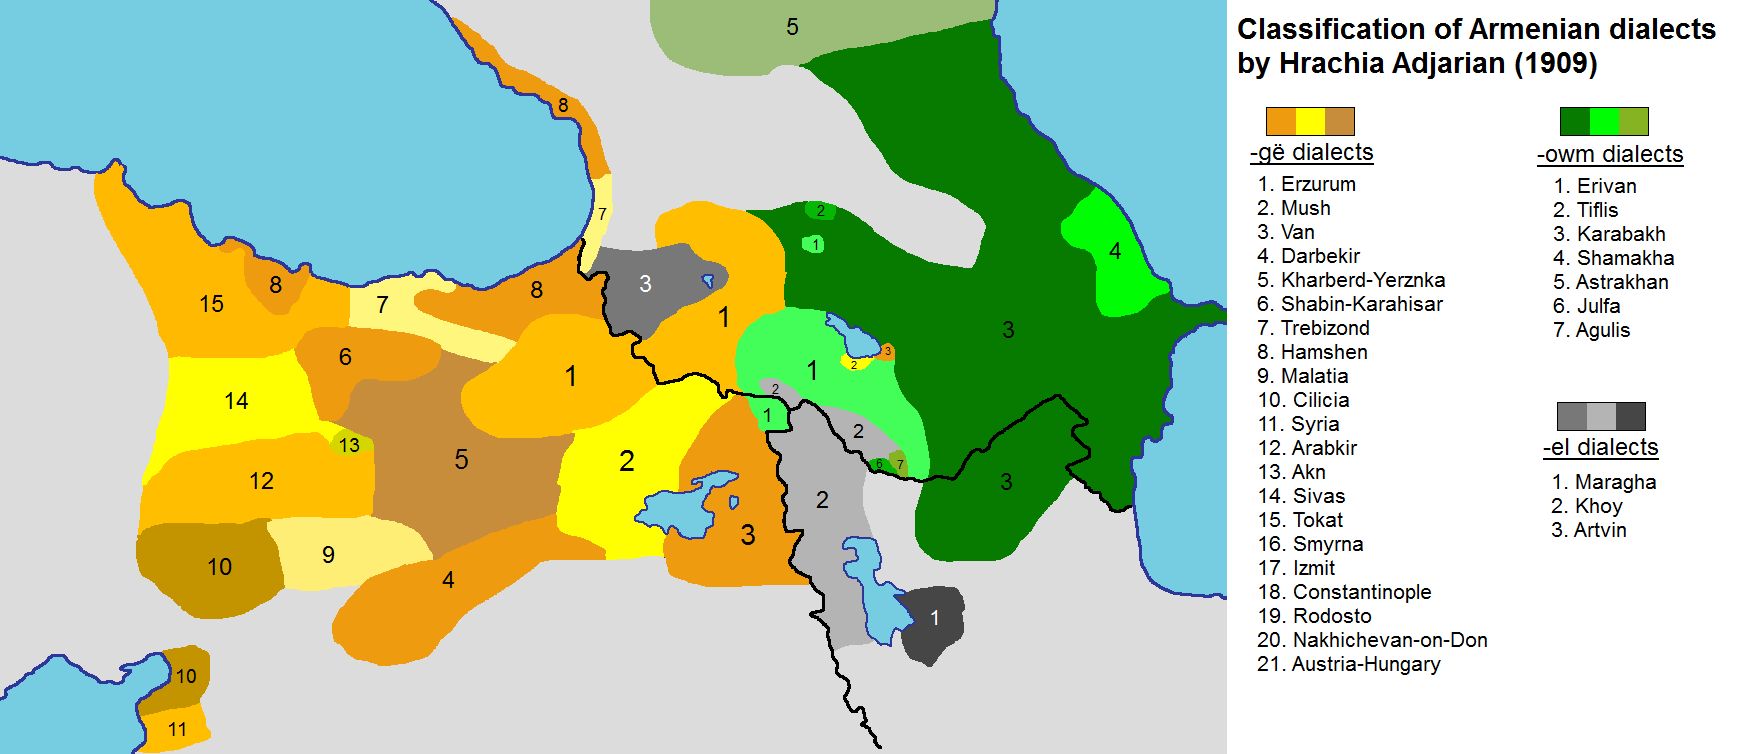
\includegraphics{images/map1909color.png}
	}
\end{figure}


\begin{landscape}
	\begin{figure} 
		\caption{Map from Adjarian 1911}
	\label{map:Adjarian1911}
	
		\centering
		%\includegraphics[width=1.0\textwidth]{Image.eps}
		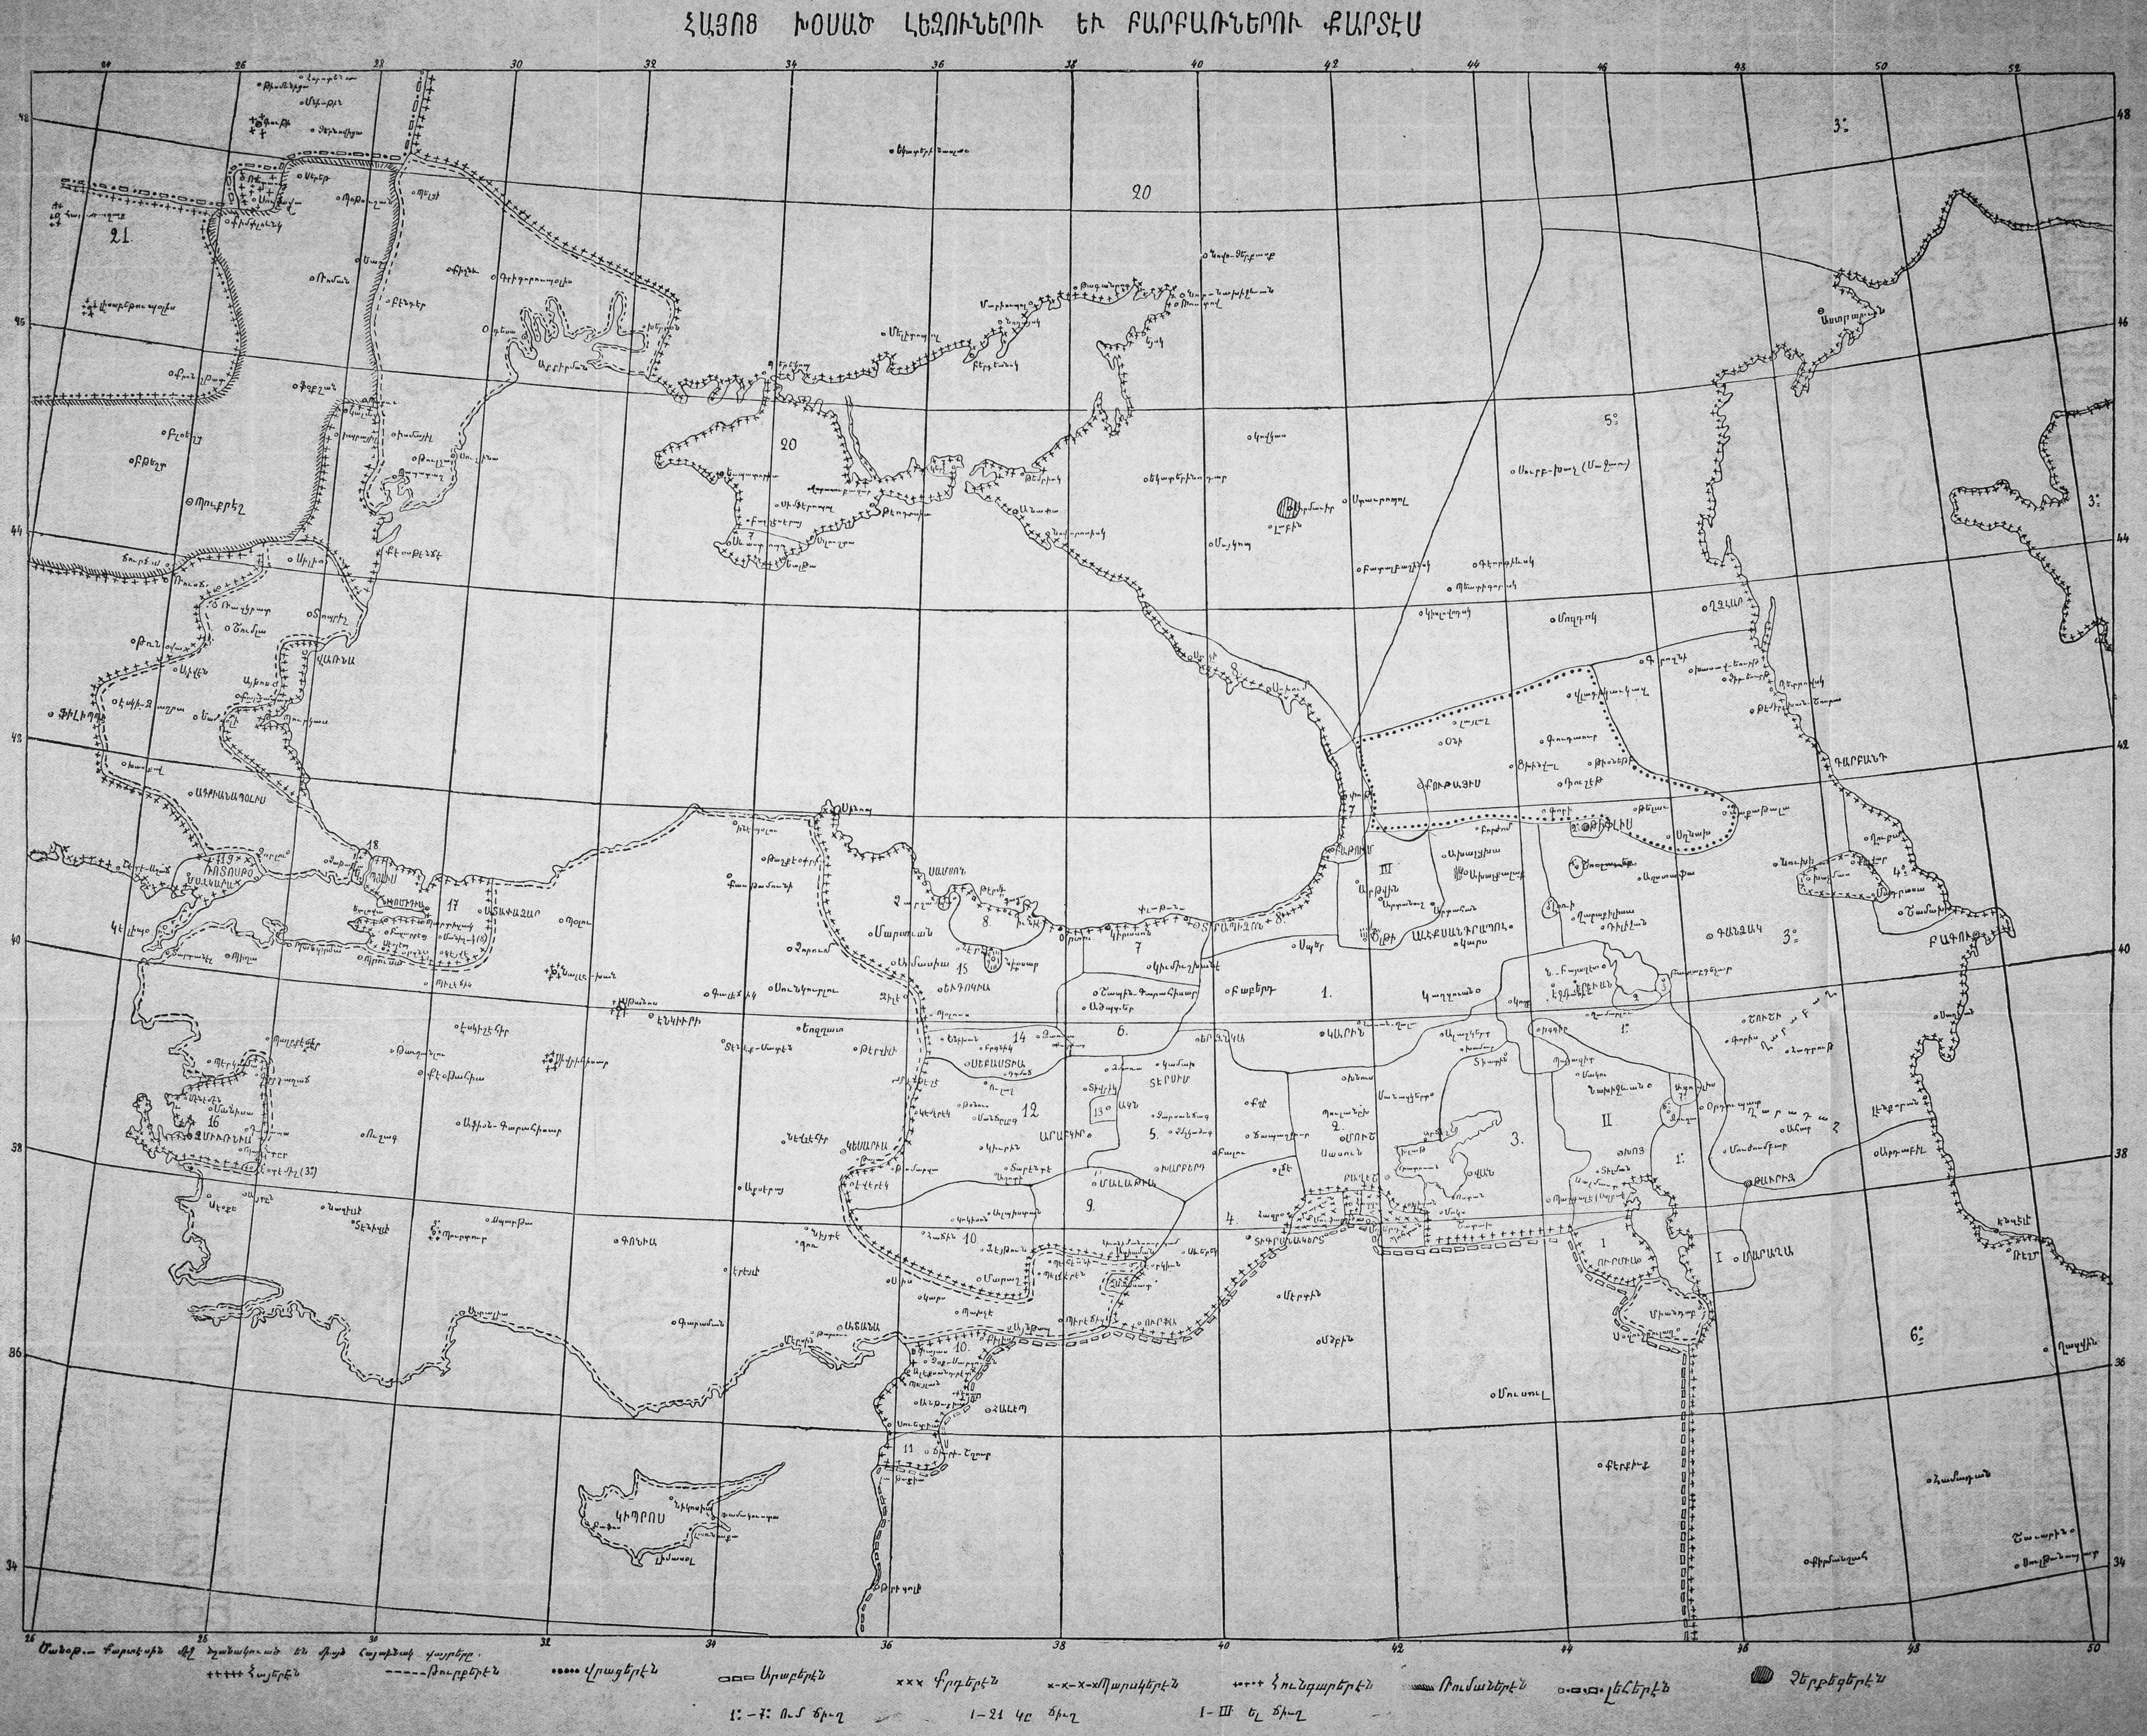
\includegraphics[height=1\textheight]{images/map1911.png}
	
	\end{figure}
\end{landscape}










\begin{landscape}
	\begin{figure}
	\caption{Map from Adjarian 1909}
\label{map:Adjarian1909}
		\centering
		%\includegraphics[width=1.0\textwidth]{Image.eps}
		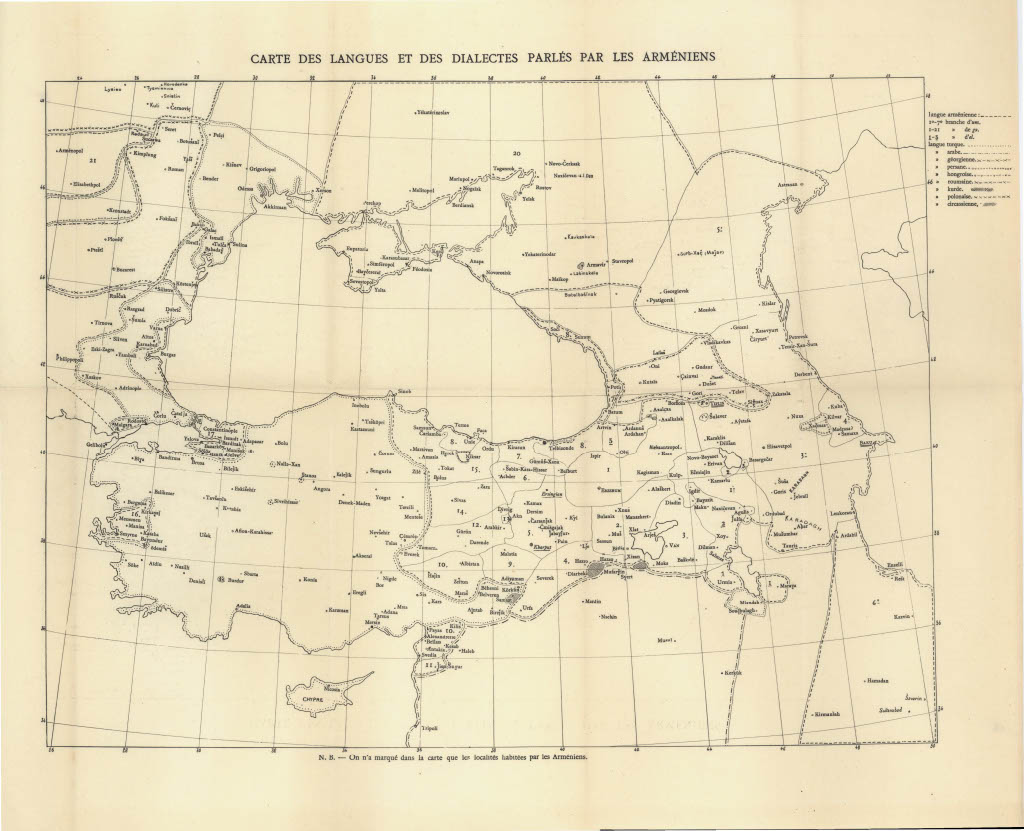
\includegraphics[height=1\textheight]{images/map1909.jpg}
		
	\end{figure}
\end{landscape}


  
 \section{Phonology of Armenian and our phonological transcription}\label{sec:HossepIntro:phonotransc}

This section explains the phonological transcriptions that I used in the translation. I explain my transcription system used for the modern standard varieties (\S\ref{sec:HossepIntro:phonotransc:modern}), Classical Armenian (\S\ref{sec:HossepIntro:phonotransc:CA}),  and non-standard dialects (\S\ref{sec:HossepIntro:phonotransc:adj}). In brief, I transcribe words in IPA based on their attested pronounciation (SEA/SWA)  or their most likely pronunciation (CA). For the non-standard dialects, Adjarian developed his own dialectological notation, for which I provide IPA approximations. 
\subsection{Phonology of Modern Standard Armenian}\label{sec:HossepIntro:phonotransc:modern}

Modern SEA and SEA are relatively well-studied in terms of their basic phonemic inventory and phonological transcriptions. I discuss nuances of transcribing SEA/SWA consonants (\S\ref{sec:HossepIntro:phonotransc:modern:cons}), vowels (\S\ref{sec:HossepIntro:phonotransc:modern:vowe}),  and stress (\S\ref{sec:HossepIntro:phonotransc:modern:stress}). 
\subsubsection{Consonant inventory}\label{sec:HossepIntro:phonotransc:modern:cons}
Table \ref{fig:HossepIntro:consSEA} provides the consonant inventories for SEA and SWA. Parentheses mark consonantal phonemes that are present in SEA but not SWA. 

\begin{table}[H]
	\caption{Consonant inventory of SEA and SWA}\label{fig:HossepIntro:consSEA}
	\resizebox{\textwidth}{!}{%
			\begin{tabular}{| l| lllllllll|}
			\hline 	& Bilabial & Labio- & Dental & Alveolar & Post- & Palatal & Velar & Uvular & Glottal \\
 & &dental & & &alveolar & & && \\
			\hline 	Stop & (p) pʰ b & & (t) tʰ d & & & & (k) kʰ ɡ & & \\
		Affricate & & & (t͡s) t͡sʰ  d͡z & & (t͡ʃ)  t͡ʃʰ  d͡ʒ & & & & \\
		Nasal & m & & & n & & & & & \\
		Trill & & & & (r) & & & & & \\
		Tap & & & & ɾ & & & & & \\
		Fricative & & f v & & s z & ʃ ʒ & & & χ ʁ & h \\
		Approximant & & & & & & j & & & \\
		\hline 
	\end{tabular}
}
\end{table}

Phonologically, SEA has a three-way larnygeal contrast or voicing contrast among stops and affricates: voiced, voiceless unaspirated, and voiceless aspirated. Classical Armenian (CA) is argued to have had a similar three-way contrast as well. In contrast, SWA has a simpler two-way contrast: phonologically voiced and phonologically voiceless (Table \ref{tab:intro:ea wa differences: phono}). Conventionally, the SWA stops and affricates are treated as being voiced vs. voiceless aspirated.

\begin{table}[H]
	\caption{Three-way laryngeal contrast in SEA but not SWA}
	\label{tab:intro:ea wa differences: phono}
	\centering
	\begin{tabular}{|l|llll| lll|}
		\hline 	& CA & SEA & &  &SWA & & 
		\\
		/p/ & \textbf{p}ɑɾ& \textbf{p}ɑɾ & `dance' & \armenian{պար} & & & 
		\\
		/pʰ/ & \textbf{pʰ}ɑk & \textbf{pʰ}ɑk & `closed' &\armenian{փակ}& \textbf{pʰ}ɑk & `closed' & \armenian{փակ}
		\\
		/b/ & \textbf{b}ɑd & \textbf{b}ɑd & `duck' & \armenian{բադ} & \textbf{b}ɑɾ & `dance'& \armenian{պար} \\ \hline
	\end{tabular}
\end{table}

However, the phonetic manifestation of the SWA voicing contrast is subject to geographical variation due to language contact \citep{kellyKeshishian-2021-VoicingWesternArmenian,Tahtadjian-2021-PhoneticInterferenceProductionStopsWesternArmenianBilingual}. For example, the SWA-speaking community in Turkey has a voiced vs. voiceless aspirated distinction for stops and affricates: D vs. Tʰ, and D͡Z vs. T͡Sʰ. In contrast, the SWA-speaking community in Lebanon instead has a voiced vs. voiceless unaspirated distinction for stops and affricates : D vs. T, and D͡Z vs. T͡S. For this monograph, because Adjarian's socio-geographic subdialect of SWA had a traditional D-Tʰ distinction, I transcribe the SWA forms with a traditional D-Tʰ distinction. 

The change from a three-way contrast in CA to a two-way contrast in SWA is a major topic in the diachronic phonology of Armenian. Throughout this translation, Adjarian spends time on describing the consonantal changes for the various non-standard dialects. 


What follows  are minor comments on the  phonology or phonetics of the consonant inventory, based largely on recent survey-level phonetic work on SEA and SWA \citep{Seyfarth-JIPAArmenian}. 


\begin{itemize}
	\item Minor comments on SEA and SWA consonant inventory 
	\begin{enumerate}
		\item The coronal stops usually have a dental articulation. 
		\item The dorsal fricatives /χ, ʁ/ are typically described as uvular, but they can have a velar pronunciation. 
		\item SEA has a phonemic trill and tap/flap distinction /r, ɾ/, while modern SWA only has a flap /ɾ/. However, more archaic registers have a phonemic trill that has been largely lost for most modern communities \citep{Tahtadjian-2020-WesterArmenianRhoticDifferentialPhoneticStudy}. Adjarian 1911 however says that SWA still has a trill in his time (Table \ref{tab:intro:othersound}).  Out of respect for Adjarian's ideolect, I thus transcribe SWA forms in this translation with a trill. 
		\item Both dialects   have an allophonic sound [ŋ]. This velar nasal is used when a nasal /n/ precedes a velar stop, i.e., there is velar place assimilation. For SEA and SWA, I transcribe the velar stop. For example, the word /menkʰ/ `we' <\armenian{մենք}> is pronounced [meŋkʰ] in SEA/SWA.  
		
	\end{enumerate}
\end{itemize}

\subsubsection{Vowel inventory}\label{sec:HossepIntro:phonotransc:modern:vowe}
Table \ref{fig:HossepIntro:SEAvowel inventory} provides the vowel inventories of SWA and SEA. Parentheses mark vowels that are present in SWA but not SEA. 

\begin{figure}[H]
	\centering
	\caption{Vowel inventory of SEA and SWA}
	\label{fig:HossepIntro:SEAvowel inventory}
	\begin{tikzpicture}[scale=2]
		\large
		\tikzset{
			vowel/.style={fill=white, anchor=mid, text depth=0ex, text height=1ex},
			dot/.style={circle,fill=black,minimum size=0.4ex,inner sep=0pt,outer sep=-1pt},
		}
		\coordinate (hf) at (0,2); % high front
		\coordinate (hb) at (2,2); % high back
		\coordinate (lf) at (1,0); % low front
		\coordinate (lb) at (2,0); % low back
		\def\V(#1,#2){barycentric cs:hf={(3-#1)*(2-#2)},hb={(3-#1)*#2},lf={#1*(2-#2)},lb={#1*#2}}
		
		% Draw the horizontal lines first.
		\draw (\V(0,0)) -- (\V(0,2));
		\draw (\V(1,0)) -- (\V(1,2));
		\draw (\V(2,0)) -- (\V(2,2));
		\draw (\V(3,0)) -- (\V(3,2));
		
		% Place all the unrounded-rounded pairs next, on top of the horizontal lines.
		\path (\V(0,0)) node[vowel, left] {i} node[dot] {};
		% \path (\V(0,1)) node[vowel, left] {ɨ} node[vowel, right] {ʉ} node[dot] {};
		\path (\V(0,2)) node[vowel, right] {u} node[dot] {};
		\path (\V(0.5,0.4)) node[vowel, right] {(ʏ)} node[dot] {};
		% \path (\V(0.5,1.6)) node[vowel, left] {} node[vowel, right] {ʊ} node[dot] {};
		\path (\V(1,0)) node[vowel, left] {e}   node[dot] {};
		%\path (\V(1,0)) node[vowel, left] {e} node[vowel, right] {ø} node[dot] {};
		% \path (\V(1,1)) node[vowel, left] {ɘ} node[vowel, right] {ɵ} node[dot] {};
		\path (\V(1,2)) node[vowel, right] {o} node[dot] {};
	%	\path (\V(2,0))   node[vowel, right] {œ} node[dot] {};
		% \path (\V(2,0)) node[vowel, left] {ɛ} node[vowel, right] {œ} node[dot] {};
		% \path (\V(2,1)) node[vowel, left] {ɜ} node[vowel, right] {ɞ} node[dot] {};
		% \path (\V(2,2)) node[vowel, left] {ʌ} node[vowel, right] {ɔ} node[dot] {};
		% \path (\V(2.5,0)) node[vowel, left] {æ} node[vowel, right] {} node[ ] {};
		% \path (\V(3,0)) node[vowel, left] {a} node[vowel, right] {ɶ} node[dot] {};
		\path (\V(3,2)) node[vowel, left] {ɑ} node[dot] {};
		
		% Draw the vertical lines.
		\draw (\V(0,0)) -- (\V(3,0));
		\draw (\V(0,1)) -- (\V(3,1));
		\draw (\V(0,2)) -- (\V(3,2));
		
		% Place the unpaired symbols last, on top of the vertical lines.
		\path (\V(1.5,1)) node[vowel] {ə};
		% \path (\V(2.5,1)) node[vowel] {ɐ};
	\end{tikzpicture}
\end{figure}


In general, the SWA sound /ʏ/ corresponds to an SEA /ju/ sequence. Some SWA loanwords have a vowel /œ/, but this vowel is quite marginal and found in only a handful of loanwords. 

The midvowels are sometimes transcribed as lax /ɛ, ɔ/ in the phonological literature \citep{Vaux-1998-ArmenianPhono}. But more recent phonetic work suggests that these vowels don't have an open-mid articulatory/acoustic target, but are instead close-mid /e, o/ \citep{Toparlak-2019-MAArmenianPhonetics,Seyfarth-JIPAArmenian}.\footnote{For my own SWA ears, I cannot perceive the difference between [e, ɛ], suggesting that Armenian has a generic articulatory target for midvowels.}
	
\subsubsection{Stress}\label{sec:HossepIntro:phonotransc:modern:stress}




SWA and SEA generally have final stress. If the last syllable has a non-schwa vowel, that vowel has stress (\ref{sent:HossepIntro:CA:stress:final}). But if the last syllable has a schwa, while the penultimate syllable has a non-schwa, then the penultimate syllable gets stress (\ref{sent:HossepIntro:CA:stress:penult}). 

\begin{exe}
	\ex SEA \label{sent:HossepIntro:CA:stress}
	\begin{xlist}
		\ex \gll kɑp\'ik \\
		monkey \\
		\trans `monkey' \label{sent:HossepIntro:CA:stress:final}\\
		\armenian{կապիկ}
		\ex \gll kɑp\'ik-ə \\
		monkey-{\defgloss} \\
		\trans `the monkey' \label{sent:HossepIntro:CA:stress:penult} \\
		\armenian{կապիկը}
		
	\end{xlist}
\end{exe}

There are some morphological exceptions to final stress. In early SWA, the suffix sequence /-e-i/ ({\thgloss}-{\pst}) in the imperfective past gets regular final stress. But in  most modern SWA communities, this suffix sequence gets penultiamte stress \citep{Dolatian-prep-ArmenianThemeAllomorphyOutputProsodyPeriphrasis}. It seems that in Adjarian's time, this change hadn't take place yet because Adjarian doesn't mention this irregularity. So I transcribe this SWA suffix sequence with final stress in this monograph. 

\subsection{Classical Armenian pronunciations and phonology}\label{sec:HossepIntro:phonotransc:CA}

Classical Armenian or CA is the oldest attested variety of Armenian. The earliest written records are from the fifth century. It is an ancient language, so we don't know its exact pronunciation, but we do have suggestive evidence (\S\ref{sec:HossepIntro:phonotransc:CA:approx}).  I set up my IPA transcription for  Classical Armenian for its monophthongal vowels (\S\ref{sec:HossepIntro:phonotransc:CA:mono}), diphthongal vowels (\S\ref{sec:HossepIntro:phonotransc:Classical:Diphthong}), consonants (\S\ref{sec:HossepIntro:phonotransc:CA:cons}), epenthetic schwas in consonant clusters (\S\ref{sec:HossepIntro:phonotransc:CA:schwa}), and stress (\S\ref{sec:HossepIntro:phonotransc:CA:stress}). 

 

\subsubsection{Approximating   the phonology of Classical Armenian}\label{sec:HossepIntro:phonotransc:CA:approx}
Classical Armenian (CA) is an ancient   language. We have no access to speakers, recordings, or phonetic analyses of CA. Thus, we cannot know exactly what CA sounded like. Instead, we can approximate a probable CA phonology using the following pieces of information:
\begin{enumerate}
	\item orthography and transliteration conventions
		\item traditional pronunciation
\item post-Classical phonological changes
\end{enumerate}

To clarify the above points, Classical Armenian is written using the Armenian script. The script was invented in order to write Classical Armenian. It is thus likely that the orthography is close to the pronunciation of Classical Armenian. The orthography is traditionally transliterated using the Hübschmann-Meillet-Benveniste transliteration system (HMB). Transliteration schemes can be found online, such as on Wiktionary.\footnote{\url{https://en.wiktionary.org/wiki/Wiktionary:Armenian_transliteration}} The transliteration is not a phonological nor phonetic transcription, but it does help us determine approximate IPA symbols for CA. 

As for pronunciation, although CA is a dead language, there is a conventional system for how to read CA texts. This system is called `traditional pronunciation'. It was formulated sometime after the first written record of CA. An approximate date for this formulation is between the 8th and 12th centuries (\citealt[24]{Godel-1975-IntroClassicalArmenian}; \citealt[1039]{Macak-2017-PhonoClassicalArmenian}). The formulated conventions indicate a mix of phonological patterns that were attested in CA or that developed later in the post-Classical period.

For this book, I transcribe all CA forms using IPA. I do not use transliteration. The rationale is that transliteration systems by themselves do not unambiguously reflect the most likely phonological form of CA words. In order to understand the various sound changes from CA to the modern dialects, it is more practical to transcribe both CA and modern Armenian in their phonological form, i.e, by using IPA symbols.\footnote{This concern is especially important for cases where the transliteration is utterly confusing from a phonological point of view. For example, the affricate series <\armenian{ձ, ծ, ց, ջ, ճ, չ}> is conventionally transliterated as <j, c, cʿ,  ǰ, č, čʿ> but its most likely pronunciation is /d͡z,   t͡s,    t͡sʰ,   d͡ʒ,   t͡ʃ,   t͡ʃʰ/.  The CA low vowel <\armenian{ա}> was likely a low back /ɑ/, and developed to SEA /ɑ/, and to dialectal /ɑ, æ/. The CA transliteration is <a>, and such a symbol is a front vowel /a/ in the IPA. The rhotic series <\armenian{ր, ռ}> developed to SEA /ɾ, r/, and were likely /ɾ, r/ in CA. But the transliteration as <r, ṙ> would confuse the non-trill and trilled symbols.}



\subsubsection{Monophthong vowel inventory}\label{sec:HossepIntro:phonotransc:CA:mono}

Classical Armenian has seven basic monopthong vowels. These vowels are listed in Table \ref{tab:HossepIntr:classicalVowel}. I provide the native orthographic form, the HBM transliteration, and an approximate IPA symbol. 



\begin{table}[H]
	\centering
	\caption{Monophthong vowels of Classical Armenian}
	\label{tab:HossepIntr:classicalVowel}
	\begin{tabular}{|l|lllllll|}
		\hline 
		Orthography & \armenian{ա} & \armenian{ե} & \armenian{է} & \armenian{ը}& \armenian{ի} & \armenian{ո} & \armenian{ու}\\
		HMB transliteration & a & e & ē & ə & i & o & u \\
		IPA transcription & ɑ & e & ē & ə & i & o & u 
		\\ \hline
	\end{tabular}
\end{table}



For the IPA transcription of Classical Armenian vowels, I adapt conventional transcriptions from the traditional pronunciation and from the modern standard dialects in the following way. 


For the grapheme <\armenian{ա}>, the modern standard dialects use a low back unrounded vowel /ɑ/. We don't know exactly what the ancient language used. For simplicity and illustration, I assume the Classical low vowel was likewise back. This seems to be an implicit assumption by Adjarian as well, because he later uses a different symbol <\armenian{ա}̈> to mark the low front vowel /æ/. 

For the front midvowel pair <\armenian{ե, է}>, we don't know the exact phonetic difference in Classical Armenian. The two graphemes are often transliterated as <e> vs. <ē>, and they are argued to have a phonological contrast in terms of tenseness \citep[14]{Thomson-1989-IntroClassicalArmenian} or length \citep[6]{Godel-1975-IntroClassicalArmenian}. Some  possible transcriptions are /ɛ/ vs. /e/,  or /e/ vs. /eː/. 

Within the IPA, the macron   ̄  indicates tone but philology often uses a macron to indicate long vowels and heavy syllables. This philological tradition is likely the reason why the HBM transliteration uses /ē/. For this translation,   I transcribe the two vowels as /e/ vs. /ē/, in keeping with the transliteration. The reason is because we ultimately don't know the actual phonological or phonetic  difference between the two vowels. All we need to know is that one vowel (the tense or long \armenian{է}) is considered the `marked' form. 


For the midvowels <\armenian{ե, ո}>, the modern standard dialects can range between using low-mid /ɛ,ɔ/ and high-mid /e,o/. Such variation is free variation in my experience. For simplicity, I transcribe them high-mid /e,o/ instead of low-mid /ɛ,ɔ/, contra \citet[1039]{Macak-2017-PhonoClassicalArmenian}. 

The segments <\armenian{ը, ի, ու}> are transliterated and traditioally pronounced as /ə, i, u/. 

\subsubsection{Diphthong vowel inventory}\label{sec:HossepIntro:phonotransc:Classical:Diphthong}
In addition to monophthongal vowels, Classical Armenian had nine diphthongs (Table \ref{tab:HossepIntr:classicalDiphthong}). 


\begin{table}[H]
	\centering
	\caption{Diphthong vowels of Classical Armenian}
	\label{tab:HossepIntr:classicalDiphthong}
	\begin{tabular}{|l|lllllllll|}
		\hline 
		Orthography & \armenian{այ} & \armenian{աւ} & \armenian{եա} & \armenian{եւ} & \armenian{եայ}& \armenian{եաւ}& \armenian{իւ} & \armenian{ոյ} & \armenian{ուա}\\
		HMB transliteration & ay & aw & ea & ew & eay& eaw& iw & oy & ua\\
		IPA transcription & ɑi̯ & ɑu̯ &e̯ɑ & eu̯ & e̯ɑi̯& e̯ɑu̯ & iu̯ & oi̯ & u̯ɑ
		\\ \hline
	\end{tabular}
\end{table}

Orthographically, Classical Armeinan diphthongs are made up of a) a vowel plus a glide symbol like <\armenian{այ}> <ay>, b) two vowels like <\armenian{եա}> <ea>, or c) a combination of vowels and glides like <\armenian{եաւ}> <eaw>. 

These orthographic sequences like <\armenian{այ}> <ay> were pronounced and phonologically treated as diphthongs like [ɑi̯] and not as vowel-glide sequences like [ɑj]. The evidence is the following. Philological and dialectological work uses the term `diphthong' (Armenian: [jeɾkbɑɾbɑr] <\armenian{երկբարբառ}>, literally `two-sounds' in Classical Armenian). In the modern standard languages, orthographic vowel-glide sequences like <ay> are pronouned as vowel-glides sequences /ɑj/, and philologists like Adjarian explicitly state that the standard dialects lack diphthongs (\S\ref{sec:AdjarianIntro:difference:soundChange:DiphthongLoss}). 

As for their IPA values, it is difficult to give a meaningful transcription for Classica diphthongs. I follow \citet{Macak-2017-PhonoClassicalArmenian} in placing an inverted breve under the less prominent member of the diphthong (= what would correspond to a high vowel). I note the following minor notational differences between my transcription and Macak. 

\begin{itemize}
		\item For <\armenian{եա}> <ea>, \citet[1041,1043]{Macak-2017-PhonoClassicalArmenian} suggests /i̯ɑ/ but I opted for /e̯ɑ/ because it's more faithful to the orthography. 
		\item For <\armenian{իւ}> <iw>, \citet[1041,1043]{Macak-2017-PhonoClassicalArmenian} notes that this cluster can be pronounced as either /iu̯/ or /i̯u/ depending on phonological position. I opt for a uniform /iu̯/ because Adjarian does not notice such differences.
		\item For <\armenian{ոյ}>, the traditional pronunciation is /ui̯/ \citep[1039]{Macak-2017-PhonoClassicalArmenian}. But, the orthography suggests that this digraph was pronounced as /oi̯/. 
\end{itemize}

For <\armenian{եայ}>, I could not find a pre-established convention so I use /e̯ɑi̯/. 
	
There is some ambiguity when an orthographic diphthong is pre-vocalic like <\armenian{այա}> or <\armenian{աւա}>. The HMB transliteration is just <aya, awa>. Phonologically, I suspect the offlgide would have acted as a consonantal onset /ɑjɑ, ɑwɑ/ and not as a sequence of vowels /ɑi̯ɑ, ɑu̯ɑ/. I thus transcribe such pre-vocalic diphthongs as vowel-glide sequences. However, note that Adjarian seems to phonologically treat these pre-vocalic forms as still phonologically diphthongs instead of vowel-glide sequences (\ref{page:64}). 




There are other attested orthographic vowel-vowel sequences such as <\armenian{ուէ}> <uē> in <\armenian{աղուէս}> `fox' and <\armenian{ուի}> <ui> in <\armenian{թուիլ}> `to appear'. For these, the HMB transliteration would be <aɫuēs> and <tʿuil>. Their modern SEA pronunciations would use a /v/ in place of the <\armenian{ու}>: /ɑʁves, tʰəvil/. It's unclear if historically such orthographic sequences were some type of diphthong too: /ɑɫu̯es, tʰu̯il/. But it is seems that the convention is to treat the digraph <\armenian{ու}> as a non-alternating /u/ \citep[15]{Thomson-1989-IntroClassicalArmenian}, and allow it to be part of vowel hiatus \citep[17]{Thomson-1989-IntroClassicalArmenian}. To be safe, I treat such sequences then as vowel hiatus as well: /ɑɫu.es, tʰu.il/.\footnote{It has been suggested that the initial /u/ in vowel hiatus is rendered as [əw] \citep[13]{Kim-2021-phoneticsPhonologyOldArmenianWV}. Thus CA /ɑɫues/ `fox' could have been pronounced as [ɑɫəwes].}

Note that Classical grapheme sequence <\armenian{աւ}> /ɑu̯/ became SEA /o/, and this change encouraged the use of a new letter <\armenian{օ}> in its place. Adjarian often uses the letter <\armenian{օ}> to refer the ancient diphthong. When he does use the letter <\armenian{օ}> in these contexts (such as <\armenian{մօր}> `mother.{\gen}'), I use the transliteration <ō> and the Classical pronunciation /ɑu̯/: <mōr>, /mɑu̯ɾ/. I usually opt to use an alternative CA spelling with <\armenian{աւ}>: <\armenian{մաւր}> <mawɾ> /mɑu̯ɾ/. I do this so that it's clearer what were the actual sound changes from Classical Armenian to the modern dialects. 


\subsubsection{Consonant inventory}\label{sec:HossepIntro:phonotransc:CA:cons}



Classical Armenian had 30 consonants (Table \ref{tab:HossepIntr:classicalConsonant}). 

\begin{table}[H]
	\centering
	\caption{Consonants of Classical Armenian}
	\label{tab:HossepIntr:classicalConsonant}
	\begin{tabular}{|l|lllllllll|}
		\hline 
		Orthography & \armenian{բ} &\armenian{պ}& \armenian{փ} &\armenian{դ}& \armenian{տ} &\armenian{թ}& \armenian{գ}& \armenian{կ}& \armenian{ք} \\
		HMB transliteration & b &p& pʿ &d& t &tʿ& g& k& kʿ \\
		IPA transcription & b &p& pʰ &d& t &tʰ& ɡ& k& kʰ \\
		\hline 
		Orthography &\armenian{ձ}& \armenian{ծ}& \armenian{ց} &\armenian{ջ}& \armenian{ճ}& \armenian{չ} & & & \\
		HMB transliteration &j &c &cʿ& ǰ &č &čʿ & & & \\
		IPA transcription & d͡z & t͡s & t͡sʰ & d͡ʒ & t͡ʃ & t͡ʃʰ & & & \\
		\hline 
		Orthography & \armenian{վ} & \armenian{ս}& \armenian{զ}& \armenian{շ}& \armenian{ժ}& \armenian{խ} & \armenian{հ} & & \\
		HMB transliteration & v & s& z& š& ž& x & h & & \\
		IPA transcription& v & s& z& ʃ& ʒ& χ & h & & 
		\\ 
		\hline
		Orthography & \armenian{մ} & \armenian{ն} & \armenian{ր}& \armenian{ռ}& \armenian{լ}& \armenian{ղ} & \armenian{ւ} & \armenian{յ} & \\
		HMB transliteration & m & n & r & ṙ&l & ł & w & y & \\
		IPA transcription & m & n & ɾ & r& l & ł & w & j& 
		\\ \hline 
	\end{tabular}
\end{table}

For stops and affricates, Classical Armenian had a three-way laryngeal contrast. This contrast is conventionally treated as between voiced, voiceless unaspirated, and voiceless aspirated /b, p, pʰ/. 

The fricatives are generally uncontroversial. 		 For the back fricative <\armenian{խ}>, the modern standard dialects show free variation between a velar /x/ vs. uvular /χ/ articulation. The uvular transcription is however more typical. I use the uvular form as the default transcription for Classical Armenian. 

For the nasals, the modern standard dialects have an allophonic velar nasal [ŋ] that's used when a coronal nasal /n/ precedes a velar stop. The Armenian orthography does not mark this in any variety, including Classical Armenian. It is unknown if Classical Armenian likewise had nasal place assimilation before velar stops, but it is likely. To be safe, I don't use a velar nasal [ŋ] for Classical Armenian. 

For the rhotics <\armenian{ր,ռ}> or <r, ṙ>, they are pronounced as a flap vs. trill in   modern SEA /ɾ, r/. It's unclear if the <\armenian{ր}> was a flap /ɾ/ or an approximant /ɹ/ in the Classical language \citep[1040]{Macak-2017-PhonoClassicalArmenian}. I opt for a flap /ɾ/. Adjarian himself does not comment on the pronunciation of this rhotic. 


For the liquids, the symbol <\armenian{լ}> <l> is pronounced as a simple lateral /l/ in the traditional pronunciation and the modern standard dialects. The symbol <\armenian{ղ}> <ɫ> is pronounced as a voiced uvular fricative /ʁ/ in the modern standard dialects, while it is generally treated as a dark or velar lateral /ɫ/ in Classical Armenian (\S\ref{sec:AdjarianIntro:difference:soundChange:VelarGlide}, \citealt[ch2]{Macak-2016-StudiesClassicalModernArmenianPhono}).

For the sonorants <\armenian{յ, ւ}>, these are traditionally transliterated as <y,w>. These sounds are the glides /j,w/. However, it is difficult to know when such a letter was pronounced as a glide vs. part of a diphthong (\S\ref{sec:HossepIntro:phonotransc:Classical:Diphthong}). 

\subsubsection{Schwa epenthesis}\label{sec:HossepIntro:phonotransc:CA:schwa}


Classical Armenian has a schwa symbol <\armenian{ը}> /ə/. This vowel is written in some words like /əst/ <\armenian{ըստ}> <əst> `for'. However, it is likely that the sound /ə/ was pronounced in many words but was unwritten in the orthography. 

In the modern standard dialects, the orthography has long clusters of consonants (Table \ref{tab:HossepIntro:schwaEpen}). These clusters are broken up by schwas in pronunciation. A conventional analysis is to treat these schwas as epenthetic \citep{Vaux-1998-ArmenianPhono}. The patterns for epenthesis are complicated but rule-governed \citep[cf.][]{Dolatian-prep-Schwa}. It is likely that these epenthetic schwas were present likewise in Classical Armenian. 



\begin{table}[H]
	\caption{Schwa epenthesis in Classical Armenian and the standard dialects} \label{tab:HossepIntro:schwaEpen}
	\centering 
	\begin{tabular}{|l| lll| l|}
		\hline `fire'	& CA & SEA & SWA & \\
		<krak> & k\textbf{ə}ɾɑk &k\textbf{ə}ɾɑk &ɡ\textbf{ə}ɾɑɡ & \armenian{կրակ}
		\\\hline 
	\end{tabular}
\end{table}

There are various reasons to assume that Classical Armenian had the same unwritten schwa epenthesis rules as the modern standard dialects. In the traditional pronunciation, the convention is to pronounce unwritten schwas in almost exactly the same places as their modern forms (\citealt[16]{Godel-1975-IntroClassicalArmenian}; \citealt[116]{Thomson-1989-IntroClassicalArmenian}; \citealt[1043]{Macak-2017-PhonoClassicalArmenian}). Diachronically, some of these unwritten schwas are reflexes of Proto-Indo-European full vowels, that got reduced in Proto-Armenian \citep[26]{Vaux-1998-ArmenianPhono}. There is no synchronic evidence of an unreduced vowel in the underlying form for these unwritten epenthetic schwas.

There have been a few attempts at formalizing the rules for pronouncing these unwritten schwas for Classical Armenian \citep{Hammalian-1984-PhonoOldArmenian,Schwink-1994-ArmenianSchwaLexicalized,Pierce-2007-SchwaClassicalArmenian}. \citet{Pierce-2007-SchwaClassicalArmenian} has noted that as a spelling-pronunciation rule, essentially the same schwa epenthesis rules are active for Classical Armenian and for Modern Armenian.

Because of the above facts, I transcribe Classical Armenian with essentially the same epenthetic schwas that the modern standard dialects use. There are some situations where the traditional prononuciation of Classical Armenian   uses an epenthetic schwa while the standard dialects don't. Two such situations are the suffix /-kʰ/ and the prefix /z-/. 

The suffix /-kʰ/ <\armenian{ք}> is a nominalizer in SEA and SWA. In the modern language, it does not use schwa epenthesis after stops or two consonants: [pɑɾt-kʰ] `debt' <\armenian{պարտք}>. But there are ambiguous and contradictory reports that the CA ancestor form (the plural suffix \textit{-kʰ}) does use schwa epenthesis in more contexts than SEA/SWA. For example, \citet[18-19]{Godel-1975-IntroClassicalArmenian}'s prose suggests schwa epenthesis applies after a CC cluster [pɑɾt-əkʰ] or after a stop/affricate. In contrast, \citet[120]{Thomson-1989-IntroClassicalArmenian}'s prose suggests no schwa epenthesis after a CC cluster [pɑɾt-kʰ]. Thomson suggests that schwa epenthesis applies only if the /-kʰ/ follows a velar stop. For these limited cases where schwa epentheiss is unclear, I transcribe the CA forms with a question mark: [pɑɾt-(ə?)kʰ]. 

The prefix /z-/ was an accusative prefix in Classical Armenian. When this prefix is before a consonant, a schwa is added before the prefix: /z-CV/$\rightarrow$[əz-CV] \citep[116]{Thomson-1989-IntroClassicalArmenian}. This prefix   is found in some archaic accusative pronouns in SWA [əz-mez] <\armenian{զմեզ}> `me.{\acc},' but it is not used as an inflectional prefix on nouns in  SWA or SEA. 




\subsubsection{Stress}\label{sec:HossepIntro:phonotransc:CA:stress}

 
In terms of stress, we don't have direct evidence from Classical sources. However, it is a convention to treat Classical Armenian as having the same basic stress patterns as the modern standard dialects (SEA and SWA), described in \S\ref{sec:HossepIntro:phonotransc:modern:stress}. 

Briefly, stress  is on the final non-schwa vowel of the word. in SEA an SWA. For Classical Armenian, the same stress rules are assumed to apply (\citealt[15]{Thomson-1989-IntroClassicalArmenian}; \citealt[1043-4]{Macak-2017-PhonoClassicalArmenian}). Evidence for the existence of final stress in pre-modern Armenian is discussed in \citet{DeLisi-2018-ArmenianProsodyDiachrony}.





\subsection{Adjarian's dialectological notation}\label{sec:HossepIntro:phonotransc:adj}


In the original monograph, Adjarian set up his own notation to capture the pronunciation of words from  non-standard dialects. He called his system a `scientific alphabet'  (\S\ref{sec:IntroAdjarian:scientificAlphabet}), and he adapted it from the Armenian script. I converted his notation to IPA, as explained in \S\ref{sec:HossepIntro:phonotransc:adj:ipa}. When re-transcribing his notation, I had to make decisions on matters that Adjarian kept implicit (\S\ref{sec:HossepIntro:phonotransc:adj:implicit}). I sometimes had to diverge from Adjarian's notation because of   typographic problems (\S\ref{sec:HossepIntro:phonotransc:adj:typograph}). I discovered that Adjarian had unfortunate inconsistencies in representing diphthongs (\S\ref{sec:HossepIntro:phonotransc:adjerror}). 


\subsubsection{IPA approximations}\label{sec:HossepIntro:phonotransc:adj:ipa}

In the original monograph, Adjarian transcribed what he perceived was the pronounciation of the non-standard dialects. He devised his own notation system based off of the Armenian alphabet, by adding additional diacritics or modifying the direction of letters. I call this his dialectological notation. 

In this translation, I retained his original dialectological transcriptions and supplied  an IPA approximation. Table \ref{tab:adjIPA}  lists all the dialectological symbols that he used, along with my IPA approximation and my  prosaic description. The PDF (and source LaTeX) of the translation can be searched for the occurrences of these symbols. Adjarian's prosaic description was  helpful in determining their phonetic values.  

For consonants, I found little difficulty in rendering them into IPA. For vowels, most cases were simple to do. But some were hard to render:  
\begin{itemize}
	\item <\armenian{ըէ} /ə̟/,  see \S\ref{section:karabak:phono:segment:mono}. 
	\item <\armenian{էօօ} /œo/,  see \S\ref{section:shamakhi:phono:change:o:lengthening}. 
	\item <\armenian{օօ}> /oo/,  see \S\ref{section:shamakhi:phono:change:o:lengthening}.
	 \item <\armenian{հյ}> /hʲ/ might be a voiceless palatal fricative /ç/.
\end{itemize}


\begin{center}
\begin{longtable}{|p{2.cm} p{2cm} p{7cm}|}

		\caption{Adjarian's  dialectological notation and my IPA approximations} \label{tab:adjIPA} \\ \hline
		\hline Adjarian's notation & IPA approximation & Description \\
		\hline 
		\multicolumn{3}{|l|}{Consonants}					\\ 
\armenian{բ}	& 	b 	& 	voiced bilabial stop	\\
		\armenian{բՙ}	& 	bʰ	& 	voiced aspirated bilabial stop	\\
		\armenian{դ}	& 	d 	& 	voiced coronal (dental) stop	\\
		\armenian{դՙ}	& 	dʰ	& 	voiced aspirated coronal (dental) stop	\\
		\armenian{ձ}	& 	d͡z 	& 	voiced coronal (dental) affricate	\\
		\armenian{ձՙ}	& 	d͡zʰ	& 	voiced aspirated coronal (dental) affricate	\\
		\armenian{ջ}	& 	d͡ʒ	& 	voiced postalveolar affricate	\\
		\armenian{ջՙ}	& 	d͡ʒʰ	& 	voiced aspirated postalveolar affricate	\\
		\armenian{ֆ}	& 	f	& 	voiceless labiodental fricative	\\
		\armenian{գ}	& 	ɡ 	& 	voiced velar stop	\\
		\armenian{գՙ}	& 	ɡʰ	& 	voiced aspirated velar stop	\\
		\armenian{գյ}	& 	ɡʲ	& 	palatalized voiced velar stop	\\
		\armenian{հՙ}	& 	ħ	& 	 voiceless pharyngeal fricative	\\
		\armenian{հ}	& 	h 	& 	voiceless glottal fricative	\\
		\armenian{հյ}	& 	hʲ	& 	palatalized voiceless glottal fricative	\\
		\armenian{՚, յ̵},   \armeniang{ֈ}	& 	ɦ	& 	voiced glottal fricative	\\
		\armenian{յ}	& 	j	& 	voiced palatal glide	\\
		\armenian{կ}	& 	k 	& 	voiceless unaspirated velar stop	\\
		\armenian{ք}	& 	kʰ	& 	voiceless aspirated velar stop	\\
		\armenian{քյ}	& 	kʰʲ	& 	palatalized voiceless aspirated velar stop	\\
		\armenian{կյ}	& 	kʲ	& 	palatalized voiceless unaspirated velar stop	\\
		\armenian{լ}	& 	l	& 	voiced lateral approximant	\\
		\armenian{լՙ}	& 	lʲ	& 	palatalized voiced lateral approximant	\\
		\armenian{մ}	& 	m 	& 	voiced bilabial nasal	\\
		\armenian{ն}	& 	n 	& 	voiced coronal (dental) nasal	\\
		\armenian{պ}	& 	p	& 	voiceless unaspirated bilabial stop	\\
		\armenian{փ}	& 	pʰ	& 	voiceless aspirated bilabial stop	\\
		\armenian{ղՙ}	& 	q	& 	voiceless uvular stop	\\
		\armenian{ռ}	& 	r 	& 	voiced alveolar trill	\\
		\armenian{ր}	& 	ɾ	& 	voiced alveolar flap	\\
		\armenian{ղ}	& 	ʁ	& 	voiced uvular fricative	\\
		\armenian{ս}	& 	s	& 	voiceless alveolar fricative	\\
		\armenian{շ}	& 	ʃ	& 	voiceless postalveolar fricative	\\
		\armenian{տ}	& 	t	& 	voiceless unaspirated coronal (dental) stop	\\
		\armenian{թ}	& 	tʰ 	& 	voiceless aspirated coronal (dental) stop	\\
		\armenian{ծ}	& 	t͡s 	& 	voiceless unaspirated coronal (dental) affricate	\\
		\armenian{ց}	& 	t͡sʰ	& 	voiceless aspirated coronal (dental) affricate	\\
		\armenian{ճ}	& 	t͡ʃ	& 	voiceless unaspirated postalveolar affricate	\\
		\armenian{չ}	& 	t͡ʃʰ	& 	voiceless aspirated postalveolar affricate	\\
		\armenian{վ}	& 	v	& 	voiced labiodental fricative	\\
		\armenian{ւ}	& 	w	& 	voiced labial-velar glide	\\
		\armenian{զ}	& 	z 	& 	voiced alveolar fricative	\\
		\armenian{ժ}	& 	ʒ	& 	voiced postalveolar fricative	\\
		\armenian{ՙ}	& 	ʕ	& 	voiced pharyngeal fricative	\\
		\armenian{խ}	& 	χ	& 	voiceless uvular fricative	\\
		\hline
		\multicolumn{3}{|l|}{Vowels}			\\
		\armeniang{{ՠ}}, \armenian{ա}̈	& 	æ	& 	low front unrounded vowel	\\
		\armenian{ա̄}	& 	ɑ̃	& 	nasalized /ɑ/	\\
		\armenian{ա}	& 	ɑ 	& 	low back unrounded vowel	\\
		\armenian{աը}	& 	ɑə̯	& 	diphthong of /ɑ/ and  (offglide) /ə/	\\
		\armenian{ա}ʲ, \armenian{ա}\textsuperscript{\armenian{յ}}	& 	ɑi̯	& 	diphthong of /ɑ/ and  (offglide) /i/	\\
		\armenian{աւ}	& 	ɑu̯	& 	diphthong of /ɑ/ and  (offglide) /u/	\\
		\armenian{է}̀ or \armenian{է} ̀	& 	e̞	& 	lowered /e/	\\
		\armenian{է}	& 	e 	& 	mid front unrounded vowel	\\
		\armenian{էյ}	& 	ei̯	& 	diphthong of /e/ and  (offglide) /i/	\\
		\armenian{էʲ}, \armenian{է}\textsuperscript{\armenian{յ}}	& 	ĕi̯	& 	shortened diphthong of /e/ and (offglide) /i/	\\
		\armenian{էյ}	& 	ej, ei̯	& 	inconsistent between diphthong or vowel-glide	\\
		\armenian{էւ}	& 	eu̯	& 	diphthong of /e/ and  (offglide) /u/	\\
		\armenian{ըէ}	& 	ə̟	& 	fronted schwa	\\
		\armenian{ը}°	& 	ə̞	& 	lowered schwa	\\
		\armenian{ը}	& 	ə 	& 	schwa (mid central vowel)	\\
		\armenian{ըⁱ},  \armenian{ը}\textsuperscript{\armenian{ի}}	& 	əi̯	& 	diphthong of /ə/ and (offglide) /i/	\\
		\armenian{ի}	& 	i 	& 	high front unrounded vowel	\\
		\armenian{ե}	& 	i̯e	& 	diphthong of (offglide) /i/ and /e/	\\
		\armenian{եւ}	& 	i̯eu̯	& 	triphthong of (offglide) /i/, /e/, and (offglide) /u/	\\
		\armenian{ի}ʲ, \armenian{ի}\textsuperscript{\armenian{յ}}	& 	ii̯	& 	diphthong of /i/ and  (offglide) /i/	\\
		\armenian{ը̂}	& 	ɨ	& 	high central unrounded vowel	\\
		\armenian{օ}	& 	o	& 	mid back rounded vowel	\\
		\armenian{էօ}	& 	œ	& 	front mid rounded vowel	\\
		\armenian{է\`օ}	& 	œə̯	& 	diphthong of /œ/ and (offglide) /ə/	\\
		\armenian{էօօ}	& 	œo	& 	perhaps a dipthong of /œ/ and /o/	\\
		\armenian{էօւ}	& 	œu̯	& 	diphthong of /œ/ and  (offglide) /u/	\\
		\armenian{օը}	& 	oə̯	& 	diphthong of /o/ and  (offglide) /ə/	\\
		\armenian{օօ}	& 	oo	& 	perhaps a long vowel /o/	\\
		\armenian{օւ}	& 	ou̯	& 	diphthong of /o/ and  (offglide) /u/	\\
		\armenian{ու}	& 	u	& 	high back rounded vowel	\\
		\armenian{ուա, ւա}	& 	u̯ɑ	& 	diphthong of  (offglide) /u/ and /ɑ/	\\
		\armenian{ուէ}	& 	u̯e	& 	diphthong of (offglide) /u/ and /e/	\\
		\armenian{ուⁱ}, \armenian{ու}\textsuperscript{\armenian{ի}}	& 	ui̯	& 	diphthong of /u/ and (offglide) /i/	\\
		\armenian{ո}	& 	u̯o	& 	diphthong of (offglide) /u/ and /o/	
		\\	
		\armenian{օ̂}	& 	u̯œ	& 	diphthong of (offglide) /u/ and /œ/	
		\\	
				\armenian{իւ}	& 	ʏ	& 	high front rounded vowel	\\
				\hline
	\end{longtable}
\end{center}


\subsubsection{Implicit information on assumed phonetic values}\label{sec:HossepIntro:phonotransc:adj:implicit}
During the course of translating Adjarian and re-transcribing his data, I had to make decisions on the exact phonetic value of Adjarian's notation. I noticed that Adjarian would omit some types of information about Armenian phonology and phonetics, whether intentionally (because he implied the information) or because of ignorance (which we can never determine). I discuss my decisions here. 
\paragraph{Typical low vowel <\armenian{ա}> /ɑ/}

For the letter <\armenian{ա}>, most traditional transliteration systems use a simpler transcription as <a>. But phonetically, this letter represents a low back unrounded vowel /ɑ/ in modern Standard Western and Standard Eastern Armenian. Although we don't have access to articulatory or acoustic data on the Armenian dialects, I suspect that Adjarian is using <\armenian{ա}> to denote a back unrounded vowel as well for the following reasons. 


First, dialectological work often distinguishes a typical vowel <\armenian{ա}> against an atypical fronted form like <\armenian{ա}̈> /æ/. This suggests that even in 1911, Adjarian perceived <\armenian{ա}> as contrasting against a front <\armenian{ա}̈> /æ/ by being back. 

Second, in the IPA, the letter <a> represents a front vowel too. Thus, if I use both <a, æ>, then it can create a false impression that there's a phonemic contrast between two front vowels <a, æ>, instead of between a front and back vowel <æ, ɑ>. 

Third, Adjarian was often sensitive in his perception of subtle acoustic differences. For example, in some dialects, he gives subtle judgments by saying that the low vowel <\armenian{ա}> had a more closed mouth in the dialect of Van (\S\ref{sec:Van:phono:soundchange:monovowel:a}). This suggests that he himself felt that <\armenian{ա}> represented a back \textit{unrounded} vowel. 

However, in my own fieldwork, the dialect of Tehrani Iranian Armenian has a rounded back vowel /ɒ/ due to Persian contact \citep[\S2.1.4]{DolatianEtAl-prep-IranianGrammar}. Perceiving this rounding is quite subtle. So it is possible that some of the dialects from Iran that Adjarian studied     did in fact use a back rounded form /ɒ/ instead of a back unrounded form /ɑ/. It is impossible to know what was the case 100 years ago.
\paragraph{Front round vowels}
For the front round vowels <\armenian{իւ, էօ}>, I transcribe them as /ʏ, œ/. These are common realizations for the SWA form of these vowels. Though it's possible that some of the non-standard dialects use /y/ or /ø/. 

\paragraph{Uvular fricatives}
For the letters <\armenian{խ,ղ}>, modern SWA and SEA use uvular /χ, ʁ/. Though in the my experience, velar pronunciations are possible as free variation. Dialectological work does not distinguish velar vs. uvular pronunciations. So although I transcribe these letters consistently as uvular across the dialects, it is possible that they may be more velar in some dialects than others. 

\paragraph{Rhotics}
For the rhotic letters <\armenian{ռ,ր}>, the modern Standard Eastern pronunciation is a trill-flap distinction /r-ɾ/. Modern dialects differ in whether the transcribed <\armenian{ր}> letter is truly a flap /ɾ/ vs. an approximant /ɹ,ɻ/. For example, Standard Western and Eastern Armenian use a flap /ɾ/, while Tehrani Iranian Armenian uses an approximant /ɻ/. Dialectologists don't distinguish these flavors of /ɾ/. But to reduce confusion with the trill, I transcribe the trill as /r/, and the non-trill rhotic as /ɾ/. 


\paragraph{Glide epenthesis in vowel hiatus repair}

In SEA and SWA, the vowel hiatus between the vowels /e/ and /i/ is repaired by either a transitional or full glide /j/ (\ref{sent:HossepIntro:phonotransc:glideepenthesis}). I include this glide in my transcriptions for SWA and SEA. 

\begin{exe}
	\ex SWA \\
	\gll /jeɾkʰ-e-i-n/ $\rightarrow$ [jeɾkʰejin] \\
	sing-{\thgloss}-{\pst}-3{\pl} \\
	\trans `(If) they sing.' \label{sent:HossepIntro:phonotransc:glideepenthesis}\\
	\armenian{երգէին}
\end{exe}



The Armenian orthography does not mark glide insertion in this context. Adjarian likewise generally doesn't include this glide either in his dialectological notation. Thus, we will come across many dialectal words that are transcribed with vowel hiatus. But I think it's likely  that there was a glide in these  contexts. For example, we see instances of such apparent vowel hiatus contexts in \S\ref{sec:Tbilisi:morpho:verb:various:eImpf}. The dialectal form is transcribed with a vowel hiatus sequence [e-i] while the SEA cognate has a glide [ej-i]. 


\paragraph{Velar place assimilation}

SEA and SWA have productive nasal place assimilation before velar stops: /n/ $\rightarrow$ [ŋ] before /kʰ, k, ɡ/ (\S\ref{sec:HossepIntro:phonotransc:modern:cons}). I transcribe these allophonic velar nasals for the SEA and SWA forms. 

It is unknown if CA had an allophonic velar nasal [ŋ]. Adjarian does not acknowledge the existence of velar nasals in CA, SEA/SWA, nor the non-standard dialects. We can't know for sure if CA and the non-standard dialects had nasal place assimilation, but it is likely. To maintain a faithful translation, I don't transcribe logically possible velar nasals in the dialects, simply because we don't know for sure if these dialects had allophonic velar nasals. 

\paragraph{Level of abstraction: schwas and   voicing assimilation}\label{sec:HossepIntro:phonotransc:adj:implicit:level of abstraction}

In general, Adjarian's dialectological notation seemed reliably close to a possible surface pronunciation for words. However, I suspect that Adjarian was at times transcribing in a more abstract or broad `phonemic form' instead of a narrow phonetic form. 

Evidence comes from    how Adjarian transcribed obstruent clusters. In SWA, there is a productive constraint against having obstruent clusters that have heterogenous voicing. For example, for the root /okʰud/ `utility' <\armenian{օգուտ}>, the derivative `helpful' is pronounced [oktʰ-ɑɡɑɾ] <\armenian{օգտակար}>. Adding a suffix causes the root's vowel to disappear, and the newly created obstruent cluster assimilates to being voiceless. 

In contrast, Adjarian often has clusters with heterogenous voicing. For example in (\ref{sent:Hamshen:misc:borrowing:sentence:kosdi}), Adjarian cites a Hamshen word /koʃ-di/ <\armenian{կոշդի}> that is borrowed from Ottoman Turkish. The suffix that he spelled as [-di] is a Turkish suffix.  The modern Turkish form of this word however is <koş-tu> where the suffix has assimilated in voicing, and this is marked in the orthography. In contrast, Adjarian transcribes this suffix in its phonemic form, without voicing assimilation.

For Adjarian's data, it is unknown if words that are transcribed with heterogenous voicing like /koʃdi/ were truly pronounced with such clusters [koʃdi], or if they were pronounced with assimilation [koʃti]. We cannot know for certain how narrow or broad  Adjarian's transcriptions were. But my suspicion is that they were rather broad (phonemic). 

Another   tendency for Adjarian was that he often omitted epenthetic schwas. On page \ref{page:9} from the original translation, Adjarian transcribed the word <\armenian{վրայ}> `on' as [vɾɑ]. But, the typical transcription is [vəɾɑ] with an epenthetic schwa. Throughout the translation, I often found Adjarian transcribing words with large consonant clusters, that would otherwise require schwa epenthesis in CA and SEA/SWA. I doubt that the relevant dialects lacked schwa epenthesis. It's possible that  Adjarian omitted some of these schwas because he either a) perceived them to be too acoustically weak or short to transcribe (= a more narrow transcription), or b) he felt the schwas were too predictable to require insertion (= a more broad transcription) 



\paragraph{Stress}
In this translation, I generally do not provide stress markings for CA nor for SWA/SEA. I provide stress markings only in the following situation. Sometimes, Adjarian documents dialectal words and he includes a stress symbol <\armenian{՛}> . He does this for words or dialects that have unexpected penultimate stress. For such situations, I also provide the stress marking for the CA and SEA/SWA cognates, to emphasize the contrast. 

\subsubsection{Typographical problems}\label{sec:HossepIntro:phonotransc:adj:typograph}

While translating the book, I came across Armenian symbols that Adjarian used which I unfortunately could not faithfully replicate. These were symbols that were either absent from Unicode, or which required specialized fonts for me to use. I had to replace these symbols with approximate symbols. 

\begin{itemize}
	\item Armenian symbols that I could not replicate easily 
	\begin{enumerate}
\item For the low front vowel /æ/, Adjarian used a special symbol 
<\armeniang{{ՠ}}>. I used the  Armenian letter <\armenian{ա}̈>. This alternative symbol is also more common in post-Adjarian dialectological work. 
\item Some diphthongs were written with a superscript form of the letter <\armenian{յ}>: <\armenian{է}\textsuperscript{\armenian{յ}}, \armenian{ի}\textsuperscript{\armenian{յ}},   \armenian{ա}\textsuperscript{\armenian{յ}}>. I used a superscript <j>: 	<\armenian{է}ʲ, \armenian{ի}ʲ, \armenian{ա}ʲ>. 
\item Some diphthongs were written with a superscript form of the letter <\armenian{ի}>: <\armenian{ու}\textsuperscript{\armenian{ի}}, \armenian{ը}\textsuperscript{\armenian{ի}}>. I used a superscript <i>: 	<\armenian{ուⁱ}, \armenian{ըⁱ}>. 
\item For a lowered schwa, Adjarian used the  upside-down version of the symbol <\armenian{ը}>. I couldn't reproduce this, so I used  <\armenian{ը}°> 
	\end{enumerate}
\end{itemize}
 
To explain why I replaced these letters, consider the sound /ĕi̯/. The original Armenian rendering is \armenian{է}\textsuperscript{\armenian{յ}} with a superscript <\armenian{յ}>. The PDF can show this substring correctly as \armenian{է}\textsuperscript{\armenian{յ}}  with a superscript.  But if the reader tries to copy this string, the result is a non-superscripted form  \armenian{էյ}. The superscript form with \armenian{է}\textsuperscript{\armenian{յ}} is not recoverable because \textsuperscript{\armenian{յ}}  is not a predefined Unicode symbol. But, if the reader tries to copy 		\armenian{էʲ}, then the superscript <j> is rendered. 


\subsubsection{Diphthong inconsistencies}\label{sec:HossepIntro:phonotransc:adjerror}

During the course of the translation, I came across inconsistencies in Adjarian's dialectological notation. 

For all dialect chapters before Crimea (\S\ref{chapter:Crimea}), Adjarian would have treated the symbols <\armenian{իւ, իեւ, իը}> as  /ʏ, ii̯eu̯, iə/. But then for Crimea (\S\ref{sec:Crimea:phono:segment:dipth}), he states these symbols should be read as single diphthongs: /iu̯, i̯eu̯,  iə̯/. This creates a contradiction with his previous use of these symbols. For <\armenian{իեւ}>, the contradiction is that <\armenian{եւ}> already signifies /i̯eu̯/. 


The symbol sequence <\armenian{էյ}> is likewise ambiguous. For some dialects, he uses this symbol to denote a diphthong /ei̯/, and he explicitly says the sound is a diphthong (Karabakh: \S\ref{sec:Karabakh:phono:segments:diph}, Cilicia: \S\ref{sec:Cilicia:phono:segment:subdialect:diph}). But then for some dialects like Agulis (\S\ref{sec:Agulis:phono:segment}) and Van (\S\ref{sec:Van:phono:segment}), he states the vowels of these dialects, and does not mention a diphthong /ei̯/, yet he still provides words with the symbol sequence <\armenian{էյ}>. One can then assume that Adjarian intends for this sequence to be read as /ej/ for these dialects.  

I suspect part of this inconsistency for <\armenian{էյ}> is due to typographical errors. For the dialect of Van, Adjarian states the Vozim dialect has a diphthong <\armenian{է}\textsuperscript{\armenian{յ}}> or <\armenian{է}ʲ> /ei̯/. This diphthong is written with a superscript glide. He provides Vozim words that have both the superscript glide and the non-superscript glide: /χejlĕi̯/ <\armenian{խէյլէ}ʲ> `mirror' (Tabe \ref{tab:Van:subdialect:Vozim:i}).   For the Vozim past perfective (\S\ref{sec:Van:subdialect:vozim:verb:paradigm:pastperf}), he sometimes transcribed a past suffix as /ĕi̯/ <\armenian{է}ʲ> but other times as /ej/ <\armenian{էյ}>. Thus, I suspect that the ambiguities in Adjarian's use of <\armenian{էյ}> could all be typos for <\armenian{է}ʲ>. 


 

\section{Translation conventions}\label{sec:HossepIntro:translation}
While translating the monograph, I had to make decisions on how to convey all the implicit and explicit information in Adjarian's prose. Such information ranged from organization (\S\ref{sec:HossepIntro:translation:exp}),  Adjarian's diachronic treatment of synchronic phonology  (\S\ref{sec:HossepIntro:translation:phono}),   morphological segmentation (\S\ref{sec:HossepIntro:translation:gloss}), my naming conventions for the morphology (\S\ref{sec:HossepIntro:translation:grammatical terms}),  his personal writing style and romanizations (\S\ref{sec:HossepIntro:translation:name}),  his use of data from multiple non-Armenian languages (\S\ref{sec:HossepIntro:translation:lang}), and my own limitations (\S\ref{sec:HossepIntro:translation:limitation}).
\subsection{Structuring and explanation}\label{sec:HossepIntro:translation:exp}
For most of this translation, I tried to maintain Adjarian's original order and way of presenting information. However, there were two issues that I had to solve: section divisions and specifying diachronic changes. 


First, Adjarian usually did not use section divisions in his dialectal chapters. Thus a dialect chapter would be a single long sequence of pages without any breaks. And in his introductory chapters, Adjarian often used at most one level of section division. To make his content easier to read, organize, and access, I tried to provide extensive subsection divisions based on various linguistic themes. 

Second,  oftentimes, Adjarian did not use any special notation to differentiate the Classical pronunciation vs. the modern pronunciations.  Within the same sentence, he uses the same letters to denote both Classical and Modern pronunciations without using any special terms.  He essentially uses one system of letter-sound correspondences for Classical Armenian, and another system for the modern dialects. For example, he would say  ``The sound X is Y,'' and then expect his Armenian-literate readers to  infer that X is Classical while Y is modern. He thus leaves it up to the (Armenian-speaking and literate) reader to deduce whenever some letter is designating the ancestor of a sound vs. the actual current pronounced form. For easier reading, I use the abbreviations like CA or MA, and terms like `Classical' and `reflex, modern' to disambiguate the text.   

For example, in section \S\ref{sec:IntroAdjarian:differences:phonetic:change:midvowelfront}, he talks about how the Classical Armenian sound /ē/ became modern /e/. But he uses the same letter <\armenian{է}> for the pronunciations. Similarly in \S\ref{sec:IntroAdjarian:differences:phonetic:change:midvowelback}, the Classical sound /o/ became a diphthong /u̯o/ in some dialects, but both phones are written with <\armenian{ո}>. The reader is expected to know that the letter <\armenian{ո}> means /o/ when used to transcribe a Classical word, while the letter means /u̯o/ when used for a modern work. 

 
\subsection{Phonological terms, changes, and  alternations}\label{sec:HossepIntro:translation:phono}
 

As discussed in \S\ref{sec:HossepIntro:phonotransc:adj:implicit:level of abstraction}, Adjarian was at times inconsistent in his phonological level of abstraction. When translating the monograph, I had to make decisions on how to represent his phonological transcriptions. I likewise came across problems in his phonological terminology and treatment.

For phonological transcriptions in this book, I generally use slashes // to encode Adjarian's transcriptions, and also for my own SWA and SEA transcriptions. This is because Adjarian's notation is ambiguously narrow or broad. I often use <> to mark orthographic transcriptions, especially in the Armenian script or in Adjarian's dialectological notation. 

In very few cases, I use brackets [] when I want to distinguish between a more abstract phonological form in slashes // vs. a more narrow phonetic form in brackets [], such as in the case of allophonic nasal place assimilation. But in general, my use of slashes // does not encode an abstract lexical representation. For example, I show epenthetic schwas in slashes //. 



Besides notation, Adjarian's treatment of Armenian phonology reflected his training in the late 19th century by Antoine Meillet. His training is substantially different from how a 21st century phonologist would look at phonology. Adjarian was trained within the framework of comparative linguistics, before the rise of Saussurian or structural linguistics (structuralistics). 


Because of his training in pre-structuralism, Adjarian does not utilize phonological concepts from structuralism such as phonemes and allophones. For example, in the Karabakh chapter, Adjarian provides a list of sounds present in the dialect (\S\ref{section:karabakh:phono:segment:list}). But he doesn't specify if all these sounds can appear freely in a word (as a phoneme), or whether certain sounds are restricted in specific contexts (as an allophone). 
	
For sounds that are borrowed from another language, he sometimes specifies that such sounds exist only in borrowed words. For example, in the Tigranakert dialect, the sound /q/ is present only in Arabic words. This sound is thus a marginal phoneme in that dialect. Yet he does not use such a theoretical term like `marginal phoneme.'

Because Adjarian was trained before the rise of structuralist or generative linguistics, he likewise didn't look at  phonology as a synchronic system of alternations. For example in the Cilicia dialect, Adjarian talks about how vowels in a word tend to assimilate (\S\ref{section:cilicia:phono:soundchange:vowelharmony}). When translating his prose, I called his process `vowel harmony' because that's how a linguist in the 21st century would understand this process, even though Adjarian didn't use such a term. 

For synchronic processes like vowel harmony, Adjarian sometimes would say what was a relevant for the process (\S\ref{sec:Shamakhi:Phonology:change:vowel:harmonyschwa}). But for diachronic changes, he often would not give  any explanation. For example in the Agulis chapter, Adjarian goes through how various   vowels changed from Classical Armenian to Agulis Armenian (\S\ref{section:agulis:phono:soundchange:mono}). But such changes seem to be haphazard. For example, the  Classical vowel /ɑ/ has many reflexes in Agulis:  /ɑ, æ, o, e, œ, jœ, ɑj, u, ʏ/. Adjarian does not describe under what phonotactic or morphological conditions these different reflexes arose. And it is beyond the scope of this translation to explain these changes. 

	
 
\subsection{Glossing and morpheme segmentation}\label{sec:HossepIntro:translation:gloss}





  Adjarian generally did not morphologically segment his dialectal data, nor would he state the meaning of some word or affix. All glossing and segmentation was my own. Adjarian would usually present his data in one of three formats. 


The first format is that he would list a dialectal word and then some related non-dialectal word. The non-dialectal word would be from CA, SEA, or SWA, but he usually doesn't state where the non-dialectal word is from. In this situation, I would transcribe the dialectal word, find and transcribe the CA and SWA/SEA cognates, and place them all together. The CA form works to show a likely ancestor for the dialectal word, while the SEA/SWA form gives a sense of the divergence of the dialect's development. To illustrate,  see Table \ref{tab:Yerevan:SoundChange:Vowel:O} in  the Yerevan chapter.  


In a lot of these situations, the non-dialectal form would have been identically written in either CA or SEA/SWA. In a few cases, the forms would be different, such as for `lentil' in Table \ref{tab:Yerevan:SoundChange:Vowel:O}; Adjarian had provided the SEA form <\armenian{ոսպ}> for this word, but not the CA word. Unless Adjarian stated otherwise, I assumed that the dialectal form had the same meaning as the CA and SEA/SWA forms. 

In some cases, Adjarian would provide a non-dialectal word in its inflected form that would have only been found in SEA/SWA, not CA. For those situations, I could only provide a partial picture of what the dialectal forms were. See for example  Table \ref{tab:Yerevan:subdialect:Astabad:pretonic} from the Yerevan chapter. Adjarian provided the dialectal form for `gathered,' but this word didn't have an obvious reflex in CA. 

Adjarian sometimes would use the asterisk * to say that a Classical word or ancestor word is reconstructed. I kept his notation. 


In very few situations, Adjarian provided a non-dialectal form that was neither in CA nor modern SEA/SWA. In those situations, I simply used the cognates that were attested. See for example the word for `cress' in Karabakh in Table \ref{tab:Karabakh:phonology:soundChange:monoph:o:u}. 


The second format was   sentences. Here, Adjarian would provide a dialectal sentence, and a SEA/SWA translation. He would not morphologically segment his sentences. However, the Armenian reader could look at the Armenian translation and figure out the closest morphological connections and segmentations. I glossed and segmented all the sentences to the best of my abilities, by deducing from the SEA/SWA translations and cognates. 

The third format was morphological paradigms. Adjarian would usually at most just list a paradigm as a set of cells and some label like `indicative present'. He usually didn't describe how such words were morphologically constructed. The Armenian reader would then have to deduce the morphological segmentation, by again contrasting against how either SWA or SEA would work to  create the indicative present. For such paradigms, I would segment the dialectal forms and provide SEA/SWA forms for easier contrast. I would prosaically explain how the SEA/SWA morphology works, and then use that information to deduce how the dialectal morphology works. For example, see \S\ref{sec:Yerevan:morpho:verb:paradigm} for the Yerevan verbal paradigms. 

I generally tried to morphologically segments as many words in possible. An exception is pronouns. I try to minimize my segmentation and glossing of pronouns because pronouns tend to contain a lot of opaque morphology. See \S\ref{section:julfa:morpho:pronoun}. 

\subsection{Grammatical termonology for morphological paradigms}\label{sec:HossepIntro:translation:grammatical terms}
 
When translating the book, I had to make decisions on how to call the different morphological items and tenses that Adjarian described. I tried to find a balance between staying faithful to Adjarian's original terminology while using the modern names for some categories. 

For example, Adjarian was often agnostic as to whether a certain morpheme was a prefix, suffix, or clitic. He often used the word <\armenian{մասնիկ}> which can be translated as `particle' or `formative.' I used the word `formative' in the translation as a way to maintain Adjarian's agnosticity. 

In his morphological paradigms, Adjarian used traditional Armenian names for the various tenses and non-finite verb forms. I go through some of the more controversial items below. 

In modern Standard Armenian, verbs can surface in a small set of non-finite verbs. The names for these non-finite forms vary based on the grammarian. For example, in Standard Eastern Armenian, the suffix \textit{-um} is used to mark a non-finite form that's called the `present participle' \citep[212]{DumTragut-2009-ArmenianReferenceGrammar} or the `imperfective converb' \citep[109]{DolatianEtAl-prep-IranianGrammar}. The word `converb' in this context is used to mean a non-finite form that can only be used in periphrastic constructions. Adjarian seems to not use any special Armenian term for this non-finite form, and tends to just say something along the lines of `with formative /-um/.'  Similarly, Standard Eastern Armenian uses the suffix /-el/ to create a non-finite form  that has been called the `perfect participle' \citep[213]{DumTragut-2009-ArmenianReferenceGrammar}, the `perfective converb' \citep[111]{DolatianEtAl-prep-IranianGrammar}, or the `past participle' (\armenian{անցեալ դերբայ})  by Adjarian (\S\ref{sec:Shamakhi:morpholgoy:verb:overview:prespastimperfectivevowels}). 

When translating the book, I stay faithful to Adjarian's prose and use the terms that he used. For example, in \S\ref{sec:Shamakhi:morpholgoy:verb:overview:prespastimperfectivevowels}, Adjarian explicitly uses the term `past participle' (\armenian{անցեալ դերբայ})  to describe a non-finite form in Yerevan, and I translate his prose as such. But, in the glossing and when discussing the SEA forms (\S\ref{section:yerevan:morpho:verb:paradigm:presentperfect}), I use more modern terminology from \citet{DolatianEtAl-prep-IranianGrammar}. The terms used in \citet{DolatianEtAl-prep-IranianGrammar} typically match the terms used in the Eastern Armenian National Corpus, with few deviations. 

There are other points of Armenian grammar that are controversial in their terminology. In Eastern dialects, the formative /k-, kə-/ is called a future prefix or formative by Adjarian. In contrast, some modern grammars of Eastern Armenian  call this a conditional future marker \citep[253ff]{DumTragut-2009-ArmenianReferenceGrammar}. We try to maintain Adjarian's terms in his prose. 

Another area worth mentioning concerns perfectivity and imperfectivity. Here, Adjarian uses traditional terms in Armenian philology which sometimes conflict  with more recent terminology in Armenian linguistics. Consider the following four sentences from Standard Eastern Armenian from Table \ref{tab:eastern perf imperf}. 

\begin{table}
	\centering
	\caption{Perfectivity and imperfectivity in Standard Eastern Armenian}
	\label{tab:eastern perf imperf}  \begin{tabular}{|lll|}
		\hline    Term from & Term from & Example \\	
		     Adjarian & \citet{DolatianEtAl-prep-IranianGrammar}  &   \\
		\hline 
		Present    &   Indicative present& siɾ-um e-n   \\
		<\armenian{ներկայ}>& & like-{\impfcvb} {\aux}-3{\pl}\\
		& & `they like, they are liking'  \\
		& & \armenian{սիրում են} \\
		\hline
		Imperfective  &   Indicative & siɾ-um ej-i-n   \\
		<\armenian{անկատար}>   & past imperfective& like-{\impfcvb} {\aux}-{\pst}-3{\pl}\\
		& & `they were liking'\\
		&  & \armenian{սիրում էին} \\
		\hline
		Perfective  &   Past perfective & siɾ-e-t͡sʰ-i-n   \\
		<\armenian{կատարեալ}>   &    & like-{\thgloss}-{\aor}-{\pst}-3{\pl}\\
		& & `they liked'\\
		&  & \armenian{սիրեցին} \\
		\hline
		Present perfect  &   Present perfect & siɾ-el e-n   \\
		<\armenian{յարակատար}>   &    & like-{\perfcvb} {\aux}-3{\pl}\\
		& & `they have liked'\\
		&  & \armenian{սիրել են} \\
		\hline
		
	\end{tabular}
	
\end{table}

A simple present tense sentence such as `they like' is simply called the `present' by Adjarian, while `indicative present' in more recent work. For marking the past tense, SEA utilizes two basic types of past constructions. One renders the incompleted past meaning of the English `they were liking,' while one renders the completed past meaning of `they liked.' The former construction is called the `imperfective'  by Adjarian, and `indicative past imperfective' by \citet[\S6.3.1]{DolatianEtAl-prep-IranianGrammar}. The latter construction is called the `(past) perfective'. More complex tenses like the present perfect are used for sentences like `they have liked.'

When translating this book, I kept Adjarian's original term in the prose. I then used the modern grammatical term in my personal section division titles and in the labels for paradigm tables.
 
When translating paradigms with Western Armenian, a problem I had was capturing the progressive tense (Table \ref{tab:prog swa}). In formal written SWA, the synthetic forms used in the indicative present and the indicative past imperfective can denote either a progresive or non-progressive reading. But in spoken SWA, the particle /ɡoɾ/ is mandatory for denoting a progressive meaning.\footnote{In SEA, there is no dedicated progressive morpheme or construction. The indicative present can have a progressive or non-progressive meaning (Table \ref{tab:eastern perf imperf}). The  indicative past imperfective has only a progressive meaning. The meaning of `I would like' is expressed by using the prefix /k-/ with past tense agreement, like [kə-siɾ-ej-i-n] \citep[\S6.5.3]{DolatianEtAl-prep-IranianGrammar}.} 

\begin{table} 
	\centering
	\caption{Progressive meanings in Standard Western Armenian}
	\label{tab:prog swa}
	\resizebox{\textwidth}{!}{%  
		\begin{tabular}{l|ll|ll}
			\hline 
			Paradigm name  & \multicolumn{2}{l|}{Example} &Literary reading & Spoken reading  \\
			\hline 
			Indicative  & ɡə-χəm-e-n& & `they drink' & `they drink'\\
			present& {\ind}-drink-{\thgloss}-3{\pl}&& `they are drinking' & 
			\\ \cline{2-5}
			& ɡə-χəm-e-n&ɡoɾ & N/A & `they are drinking'\\
			& {\ind}-drink-{\thgloss}-3{\pl} & {\prog} &&  \\
			
			\hline
			Indicative & ɡə-χəm-ej-i-n&& `they would drink' & `they would drink'\\
			past imperfective & {\ind}-drink-{\thgloss}-{\pst}-3{\pl}&& `they are drinking' &  
			\\ \cline{2-5}
			& ɡə-χəm-ej-i-n &ɡoɾ&   & `they are drinking'\\
			& {\ind}-drink-{\thgloss}-{\pst}-3{\pl}& {\prog} & &  \\ \hline
		\end{tabular}
	}
\end{table}

Outside of an artificial literary context, a SWA speaker cannot naturally perceive a progressive reading for these synthetic forms without /ɡoɾ/. When translating past imperfective sentences for the Western dialects, I used the non-progressive meaning as the default (following the spoken register of SWA).  In some cases, Adjarian explicitly said a sentence had a progressive meaning; so I followed him in those contexts.


Past tense morphology presents another set of problems in Eastern Armenian. When the future prefix [k(ə)-] is added to the subjunctive present, it creates a simple future reading `I will like'. But when it's added to a subjunctive past form, it creates a conditional-like reading `I would like' \citep[\S6.5.3]{DolatianEtAl-prep-IranianGrammar}.   Adjarian calls the latter reading the future past though it's semantically inaccurate. See discussion in \S\ref{section:agulis:morph:verb:paradigm:future}. 
 

 
\subsection{Cultural terminology and names used by Adjarian}\label{sec:HossepIntro:translation:name}

There were minor cases where Adjarian would use an Armenian term that was dificult to translate accurately. One such word was the noun <\armenian{գաղութ}>. This word can be translated in various ways such as `colony' or `settlement'. The derived word <\armenian{գաղթական}> can then also be translated as `colonizer, settler, migrant, emigre' and so on. 

In general, he would use these two words to describe communities of Armenians who were living in areas outside of Historic Armenia, or communities who migrated across different regions and cities. Throughout this book, I tended to translate these terms as either   `settlements' or `migrant communities'. I did tihs because the word `colony' can incorrectly imply that these Armenian communities were part of some colonialization effort, instead of just normal human migration.\footnote{In the French version, \citet{Adjarian-1909-ClassificationArmenianDialect} used the French words `colonie'(page 13) and `emigration' (page 84).  I thank Bert Vaux and Thomas Castaigna for finding out for me.} 

Adjarian likewise was  sometimes flowery in his prose. He would often use the phrase <\armenian{հին հայերէն}> `Old Armenian' to denote Classical Armenian, instead of the conventional word <\armenian{գրաբար}>. He used the term <\armenian{նոր հայերէն}> `New Armenian' to denote the modern descendants (whether standard or non-standard dialects). The standard language was <\armenian{գրական}> `literary'. He likewise used the word `sea' for lakes.    I didn't alter Adjarian's word choices, to maintain faithfulness to his personal style. 

He would often use the word `ending'  (\armenian{վերջաւորութիւն}) in ambiguous ways. It could mean a word-final segment (\S\ref{section:Aguli:phono:change:cons:n}), a suffix (\S\ref{section:yerevan:morpho:verb:details:impertative}), or a suffix sequence (\S\ref{sec:Akn:morphology:verb:archaicPstPl}). 

A complicated area of translation involved the root <\armenian{տաճիկ}> pronounced /dɑd͡ʒiɡ/ in SWA, and /tɑt͡ʃik/ in SEA. This root can mean a range of related meanings like Turk or Muslim. It's used in phrases like <\armenian{տաճկերէն}> /dɑd͡ʒɡeɾen/ which is the language of those people (Turkish), <\armenian{տաճկաստան}> /dɑd͡ʒɡɑstɑn/ which is the country (Turkey), or <\armenian{տաճկահայ}> /dɑd͡ʒɡɑhɑj/ which is an Armenian from that area. In Adjarian's prose, he used this root and its derivatives to refer to the notions of  Ottoman Turks, Ottoman Turkish, Ottoman Turkey, and Ottoman Armenians. I thus translated these words as such.\footnote{Because of the genocide, I thought it would be insulting to translate the word  <\armenian{տաճկահայ}> to `Turkish-Armenian' instead of `Ottoman Armenian'.} Some related words are <\armenian{թուրք}> /tʰuɾkʰ/ and <\armenian{թրքերէն}> /tʰəɾkʰeɾen/ which mean Turk and Turkish. 

In some case, Adjarian would use a linguistic term in somewhat vague ways. The term <\armenian{պայթուցիկ}> is supposed to denote a stop consonant (= a plosive). However, he sometimes would use the word `plosive' to denote either a stop or affricate. Thus throughout the translation, there are likely sentences where I used the word `plosive],' but the phrase `stop  or affricate' may have captured his intent better. Unfortunately, his style of writing would often make using a longer phrase harder to read.  When translating \citet{Adjarian-1899-ArmenianExplosives}, Balabanian faced a similar issue (\S\ref{chapter:George}). 

A difficult matter to translate was proper names. Adjarian usually wrote people's name in the Armenian script. I would write the person's name in the original script that Adjarian used, alongside a romanization. In some cases, the person had an existing or well-known romanized name. For example, the late Armenian philologist <\armenian{Շահան Ջրպետ}> had a romanized name `Jacques Chahan de Cirbied'. 

In other cases, I couldn't find a romanized version of the  person's name online. In such cases, I made up my own unofficial romanization based on a simplified HBM transliteration. I would provide  the IPA pronounciation in SEA/SWA.  To explain why I did this, my Armenian name is <\armenian{Տէօվլէթեան}> and pronounced in SWA as [dovletʰjɑn]. Its HBM form would be <Tēōvlētʿean>, but the romanized form that I had used within the Armenian community is <Deovletian>.  The two romanizations are obviously different, and the HMB transliteration is not publicly used.

In order  to show respect to the many deceased (and likely massacred) individuals who worked with Adjarian in his documentation efforts, I wanted to romanize their names in the way that I would expect to see such names in real life and in pronounced forms.  For example, I romanized the surname suffix <\armenian{եան}> as <-ian>, because this is how people in real life romanize their names (outside of academic bibliographies), and not as the HBM form <-ean>. For affricates like <\armenian{ց}>, I wouldn't romanize them using HBM letters like <cʿ> because such symbols aren't used by Armenians outside of academic publications. I instead used symbols like <ts>. Of course, these romanized forms are ambiguous. But, I provide the original Armenians form anyway. So there is no loss of information.






\subsection{Translating language examples}\label{sec:HossepIntro:translation:lang}

In this book, Adjarian would provide linguistic examples from various languages and registers. These languages were the following.

\begin{itemize}
		 \item French
\item Italian
\item German
\item English
		 \item Russian
		 \item Georgian
		 \item Persian
\item Arabic
		 \item Ottoman Turkish
		 \item Classical Armenian
		 \item Standard Armenian, often ambiguously either SEA or SWA
		\end{itemize}
		

I only speak SWA, English, and Arabic. So when translating these examples, I used the following procedure. 

For Romance and Germanic languages, I largely relied on Wiktionary. Adjarian's examples were mostly just word lists so this was feasible. For French, I have some beginner level reading capacity. 

For Russian, I cannot read the Cyrillic script. I relied on the help of  a Russian speaker (Nikita Bezrukov) to help in the translation. 

For Persian and Arabic, I knew the Arabic script so I could use Wiktionary (and my own Arabic knowledge) to translate. Some Persian cases were difficult, so for that I had the help of a speaker (Nazilia Shafiei). 

For Georgian, I don't know the script so I relied on two linguists (David Erschler and Thomas Wier) who work on Georgian. 

For Ottoman Turkish, Adjarian usually wrote these phrases in Armenian letters. I used a combination of Wiktionary and help from Turkish speakers (Tabita Toparlak,  Nazila Shafiei, Jonathan North Washington) to translate the Ottoman forms to English and modern Turkish. 

For Classical Armenian, I relied on the Calfa dictionary\footnote{\url{https://dictionary.calfa.fr/}} and English Wiktionary. In some cases, Adjarian used a word that he implied was a Classical word but I couldn't track it down. In those situations, he would use the Classical word as a gloss for a  dialectal word. I instead used a cognate that was attested in the Classical dictionaries. 

For SWA and SEA, I relied mainly on my own native knowledge of SWA. For transcribing SEA forms, I relied on English Wiktionary. The Armenian entries on English Wiktionary are highly moderated by Vahagn Petrosyan. For SEA words whose transcriptions I couldn't find on Wiktionary, I instead asked Petrosyan for help. 


\subsection{Limitations of the translation}\label{sec:HossepIntro:translation:limitation}
 


I have tried my best to ascertain the exact translation of as much of Adjarian's prose as possible for me. At times where I was unsure on how to translate a word or phrase, I reached out to others for help. But there are still small points where I couldn't decide on a proper translation. A lot of these errors can be found in the my footnotes, which include the substring `(?)'  which  can be   searched for. 


Below I go through the types of datapoints that I couldn't  be fully confident in translating. My hope is that because this book is open-access, then future readers can contribute to ongoing translation work by finding my errors. 

In some cases, I couldn't track down the exact bibliographic entry for an academic work that Adjarian cites. This is because he doesn't provide a complete bibliography but often just mentions the author's name and year of publication. For example, see the unclear   difficult citations   for Hanusz (footnote \ref{footnote failed hanusz}) and Davit-Bek (footnote \ref{failed footnote for david bek marash}). I include the symbol `(?)' for such footnotes.

In very rare cases, the original prose was confusing and ambiguous. For example, see footnotes \ref{footnote failed translation abbr}, \ref{footnote failed translation fourth},  among others.

In some cases, Adjarian is too implicit and vague. For example, he sometimes doesn't state the dialectal or etymological origin of  some word (footnote  \ref{footnote failed translation absent dialect}). 



For the morphology,        Adjarian doesn't segment, gloss, or explain his suffixes. There are some cases where I couldn't figure out what a suffix meant. For    example, the reader can search for the substrings `-?,'  `?-,' or `(?)' to find less than a hundred cases of untranslated morphemes. Some example sentences likewise lacked a translation and I couldn't figure out what they meant. 

For placenames in the end matter, only a few places have unclear romanizations because I couldn't track down the place. These unclear placenames have a question mark. 

For the sample texts for the 31 non-standard dialects, I did not translate, gloss, or re-transcribe them. Adjarian didn't   explain his texts, and he only sometimes rendered them into his dialectological notation. It would have been to cumbersome and error-ridden for me (and for any non-speaker of the relevant dialect) to translate such samples. I encourage future researchers who focus on those specific dialects to use the open-access sources in this translation. 

This translation focuses on capturing the information that Adjarian presented in his 1911 book. Thus, I do no provide recent descriptions of those 31 dialects. But for each dialect, I provide a citation to \citet{Martirosyan-2019-ArmenianDialectsBigVersionRussianJournal}'s survey. The survey lists more recent grammars on a specific dialect. I place this citation  in the literature section (if this section exists), otherwise in the background section. 

Finally, this book is a translation of the 1911 Armenian edition which is almost 300 pages. The 1909 French version is smaller at almost 100 pages. Because I don't speak French and because the Armenian edition is substantially larger, I used the Armenian edition as the source to translate. Because I don't speak French, it's unclear to me if there's any information present in the French edition that is absent in the Armenian edition. 






\setchapterpreamble[u]
{%
	\renewcommand*{\dictumrule}{\par}
	\let\dictumwidth\textwidth
	\dictum{\normalfont\itshape\raggedleft Translated by George Balabanian}
	\bigskip\par
}


\chapter{Translation of Adjarian 1899 on voice onset time}\label{chapter:George}

	
	\translatorHD{Below is a translation of \citet{Adjarian-1899-ArmenianExplosives}, done by George Balabanian. That paper is an early acoustic demonstration of voice onset time, using Armenian data \citep{braun-2013-earlyCaseVOTAdjarian}. } 

\textbf{Original title:} Les Explosives de l'ancien arménien étudiées dans les dialectes modernes

\textbf{Translated title:} The stops and affricates of Classical Armenian, studied in modern dialects

\section{Introduction, background, and methodology}




Here, I investigate what has become of the three groups of Classical Armenian stops and affricates in the modern dialects.

\translatorHD{The French term that Adjarian uses is ``explosives,'' which is no longer used today. It was generally used in the 19th century to describe stops (plosives), and sometimes both stops and affricates (which is the way Adjarian uses it). The term `obstruent' is too wide a term, as it would include all fricatives, stridents, and sibilants. And `occlusive' is also too wide, as it also includes nasals.}



\begin{table}[H]
	\resizebox{\textwidth}{!}{%
	\begin{tabular}{llll}
			\lsptoprule Adjarian's original  & Armenian  & IPA transcription & Hübschmann-Meillet  \\
			notation & orthography &     &     transliteration \\
			 \cmidrule(lr){1-1}  \cmidrule(lr){2-2}        \cmidrule(lr){3-3}  \cmidrule(lr){4-4}      
			b, g, d, dz, dj & \armenian{բ, գ, դ, ձ,   ջ} & b, g, d, d͡z, d͡ʒ & b, ɡ, d, j, ǰ   \\
			p, k, t, ts, tch & \armenian{պ, կ, տ, ծ,   ճ} & p, k, t, t͡s, t͡ʃ & p, k, t, c, č  \\
			pᶜ, kᶜ, tᶜ, tsᶜ,   tchᶜ & \armenian{փ, ք, թ, ց,   չ} & pʰ, kʰ, tʰ,   t͡sʰ, t͡ʃʰ & pʿ, kʿ, tʿ, cʿ, čʿ  
			\\ \lspbottomrule 
		\end{tabular}
}
\end{table}


I limit my study only to word-initial sounds and to differences in sonority and intensity.

The sonority of a consonant is determined by the relationship between two moments: the moment when the consonant bursts out by the effect of the air being expelled from the mouth, and the moment when the larynx vibrates. The intensity is proportional to the amount of air expended for the explosion. To determine these various data, I used the experimental method. In other words, I had recourse to the phonetic laboratory and machines of the Abbot Rousselot.\footnote{Jean-Pierre Rousselot (1846-1924) was a French priest and is considered the founder of experimental phonetics.}

I collected the movements of the speech air column with a mouthpiece, and the vibrations of the larynx with a capsule attached to the thyroid cartilage with a rubber tie. Both phenomena were recorded on a rotating cylinder by means of two lever drums mounted to capture the vibratory movements and acting simultaneously.

Each of my plots thus consists of two synchronic lines: the top one marking the air displacement, or speech, the lower one, laryngeal vibrations.

I've indicated synchronicity by means of vertical construction lines. The dotted lines indicate when the larynx begins to vibrate; solid lines indicate the moment of burst.

All plots are comparable in terms of sound sonority. But for the various degrees of intensity, it is only legitimate to compare between plots relating to the same dialect, as my experiments were carried out at rather different times and with different equipment.



\translatorHD{Adjarian listed data from the following dialects, along with an abbreviation:}

\begin{itemize}
	\item C = Constantinople; 1 2 3 mark three variants of popular pronunciation: C1 emphatic pronunciation, C2 normal pronunciation, C3 exceptional pronunciation.
	
	\translatorHD{See the Istanbul chapter \S\ref{section:istanbul:phono:inventory:cons} and \S\ref{sec:Istanbul:phono:soundchange:cons:laryngeal}.}
	\item A = Aslanbeg 
	
	
	\translatorHD{The Aslanbeg variety is a subdialect of the Nicomedia dialect. See \S\ref{section:nicomedia:phono:inventory}.}
	\item N = Nukha
	
	\translatorHD{French spelling is Nouxa; also spelled Nukhi, Nukha; Shaki (Şəki) of modern-day Azerbaijan, \armenian{Նուխի} or \armenian{Շաքի} in Armenian, part of the Karabakh/Artsakh dialect group. For general information on the consonant system of Karabakh, see \S\ref{section:karabakh:phono:inventory:cons} and \S\ref{section:karabakh:phono:change:cons}.} 
	\item M = Mush: M1 first category of voiced consonants; M2 second category of voiced consonants.
	
	\translatorHD{For more information on Mush, see \ref{section:mush:phono:change:cons}.}
	\item Ch  = Shushi
	
	\translatorHD{Originally \textit{Ch} for \textit{Choucha} (Shushi, Shusha).} 
	
	\translatorHD{The Shushi vernacular is part of the Karabakh dialect group. For general information on the consonant system of Karabakh, see \S\ref{section:karabakh:phono:inventory:cons} and \S\ref{section:karabakh:phono:change:cons}.}
	\item S = Sivas
	
	\translatorHD{Also commonly known as Sebastia.}
	
	\translatorHD{For more information on Sebastia, see \S\ref{section:sebastia:phono:inventory:cons}.} 
	
	
\end{itemize}

 

\begin{figure}
	\centering
	\resizebox{\textwidth}{!}{%
	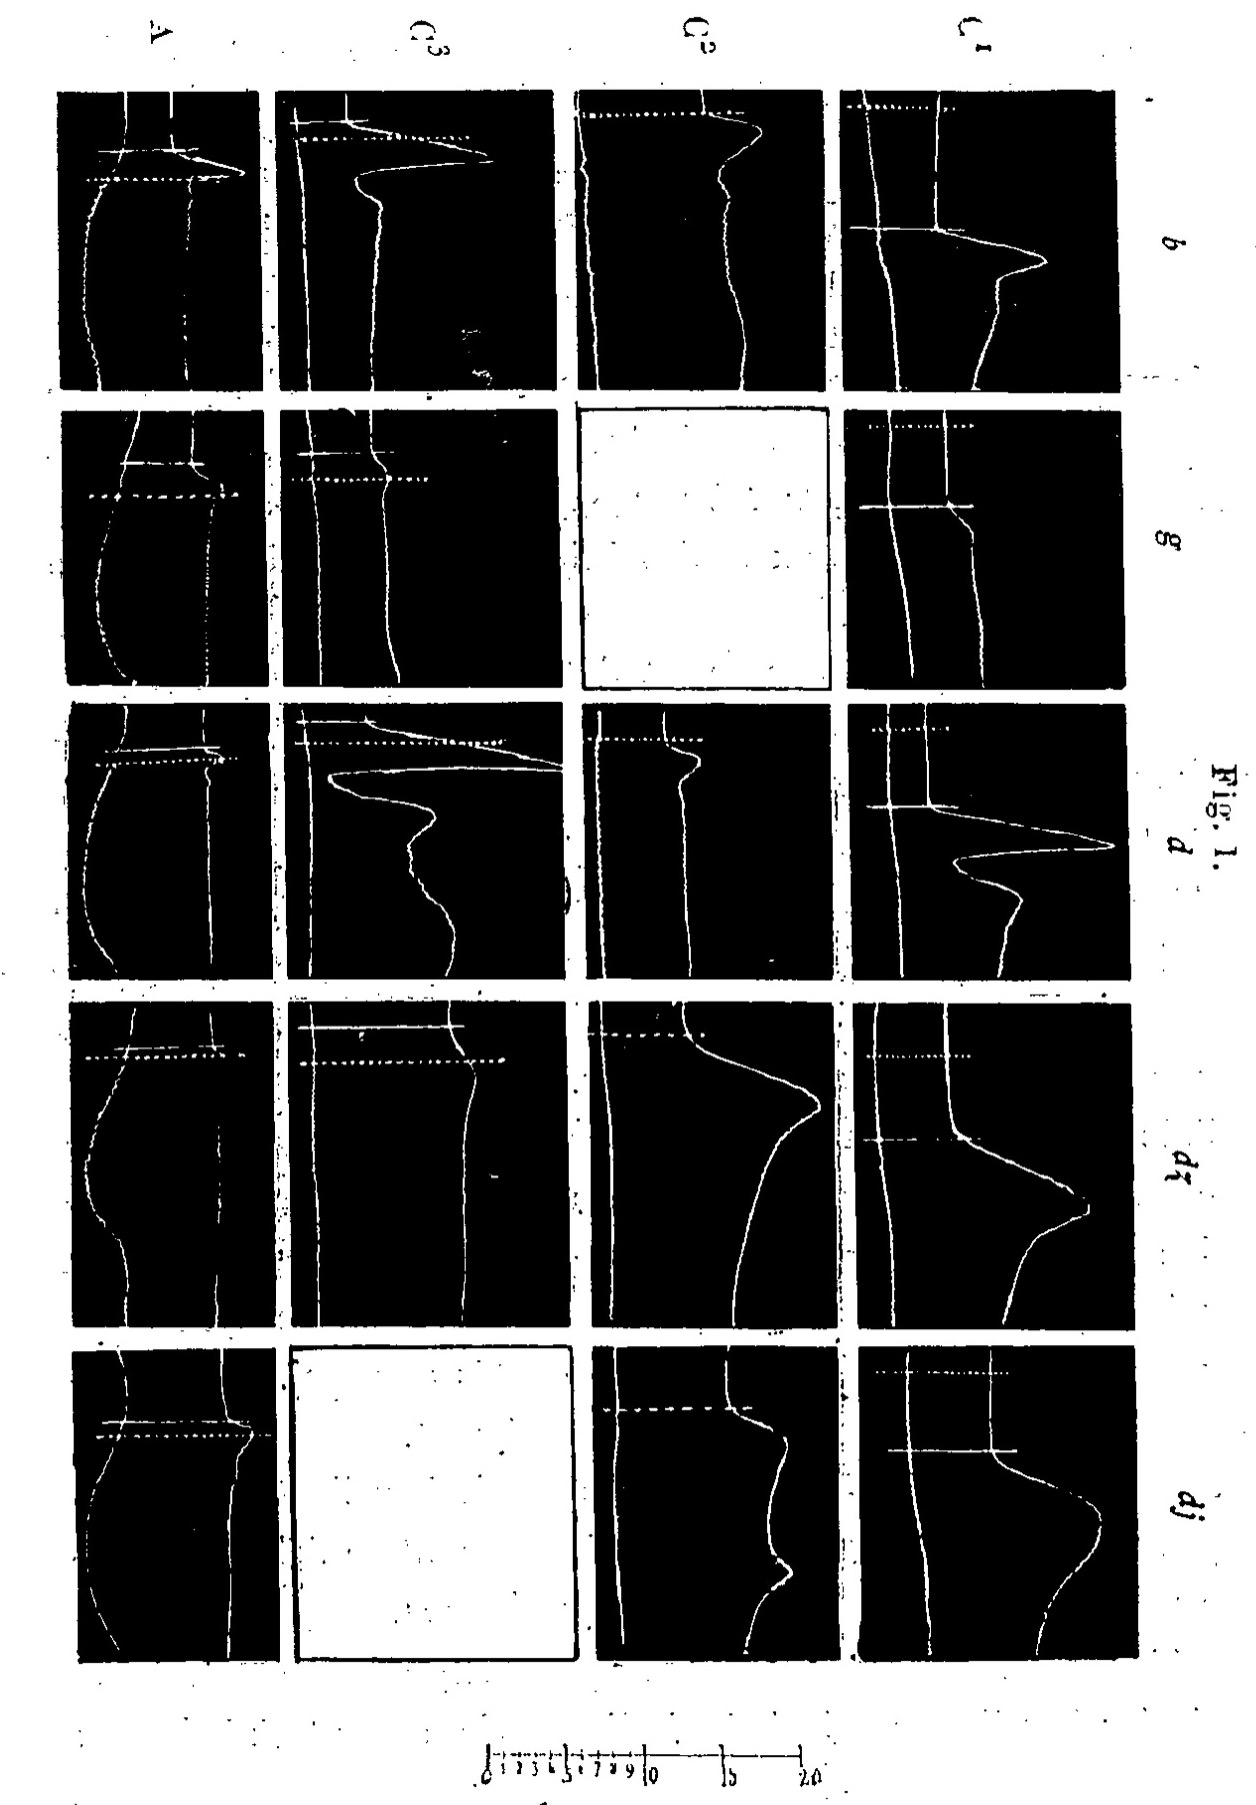
\includegraphics[scale= .3]{images/adjarian1899fig1.jpg}
}
	\caption{Original figure 1 for reflexes of Classical Armenian voiced stops and affricates}
	\label{fig:fig1 original}
\end{figure}

\begin{figure}
	\centering
	\resizebox{\textwidth}{!}{%
	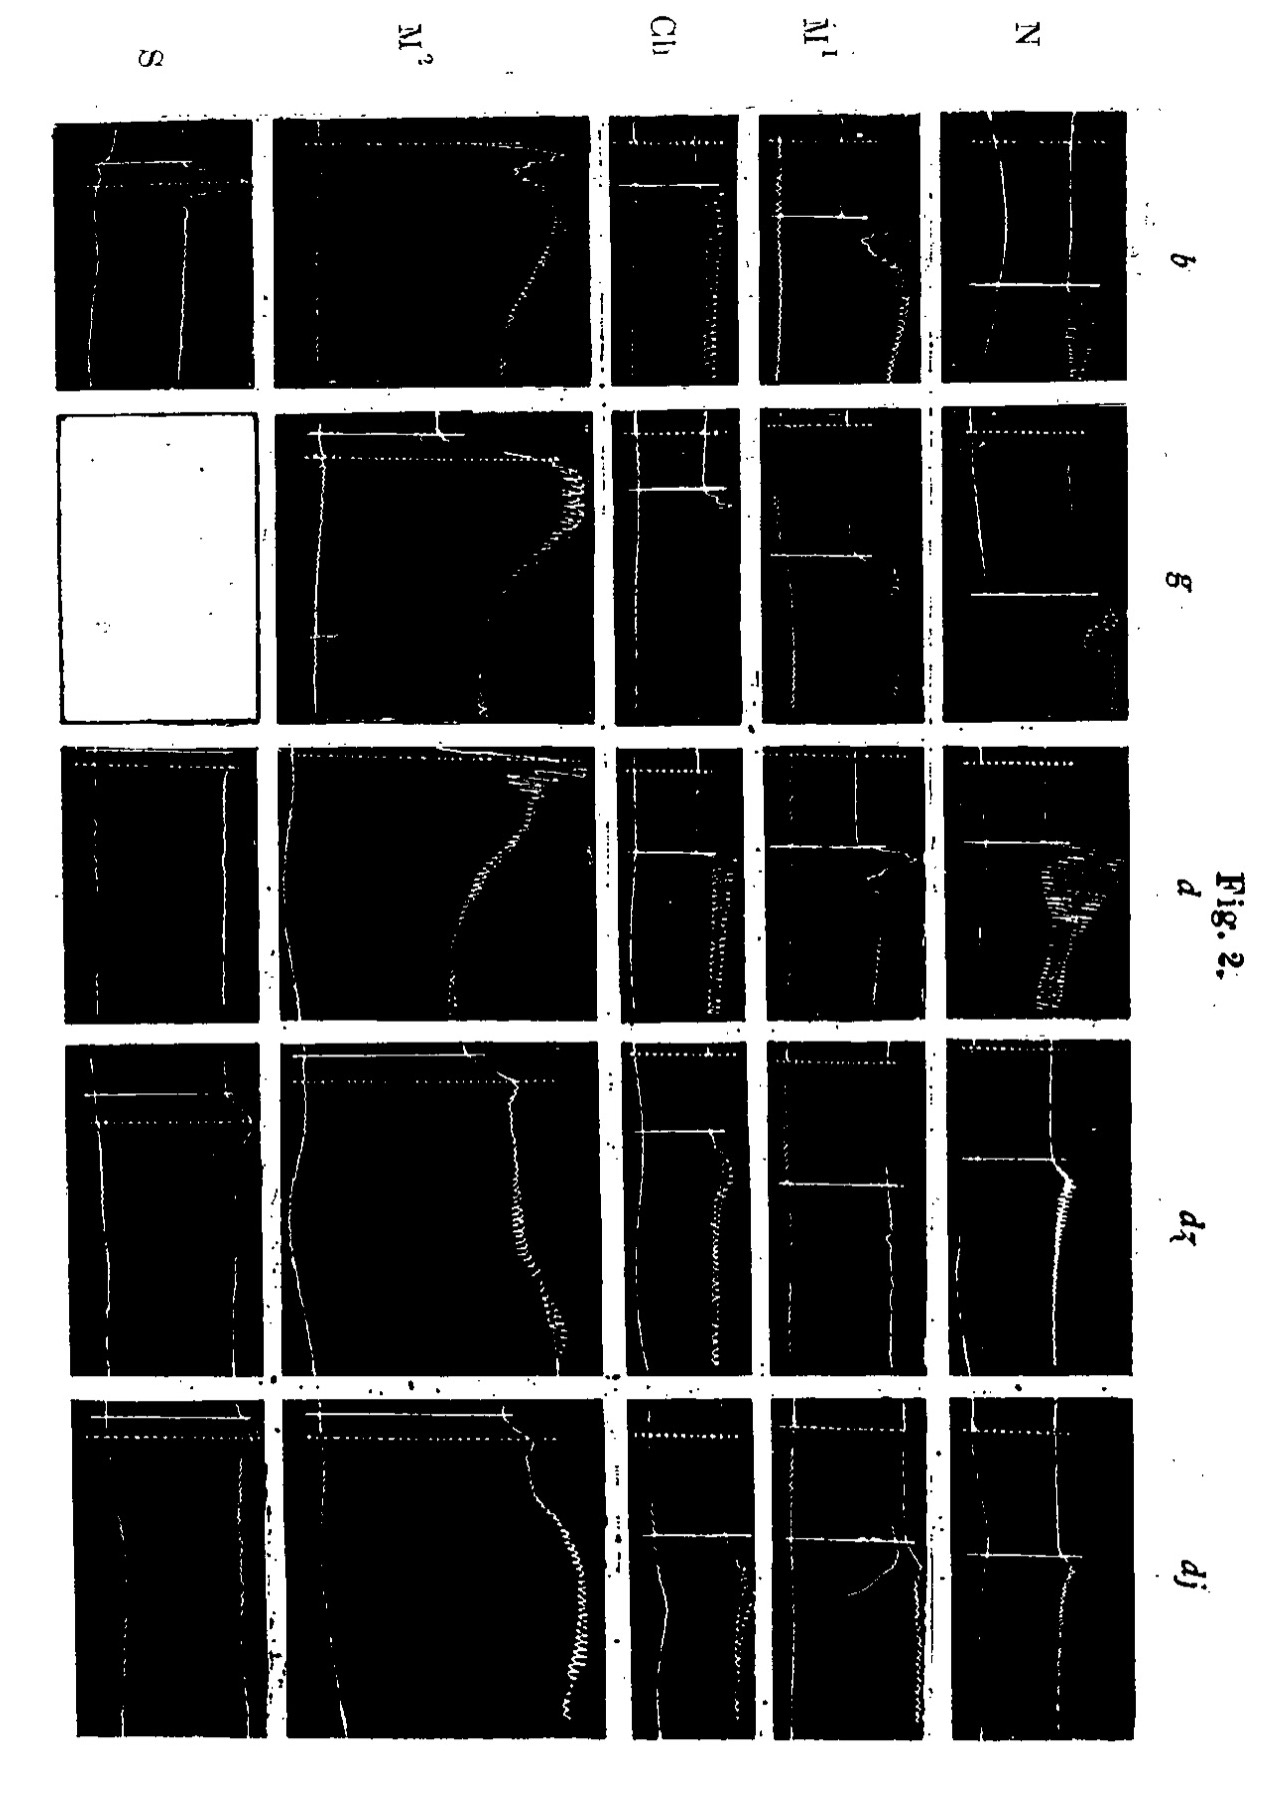
\includegraphics[scale= .3]{images/adjarian1899fig2.jpg}
}
	\caption{Original figure 2 for reflexes of Classical Armenian voiced stops and affricates}
	\label{fig:fig2 original}
\end{figure}


\begin{figure}
	\centering
	\resizebox{\textwidth}{!}{%
	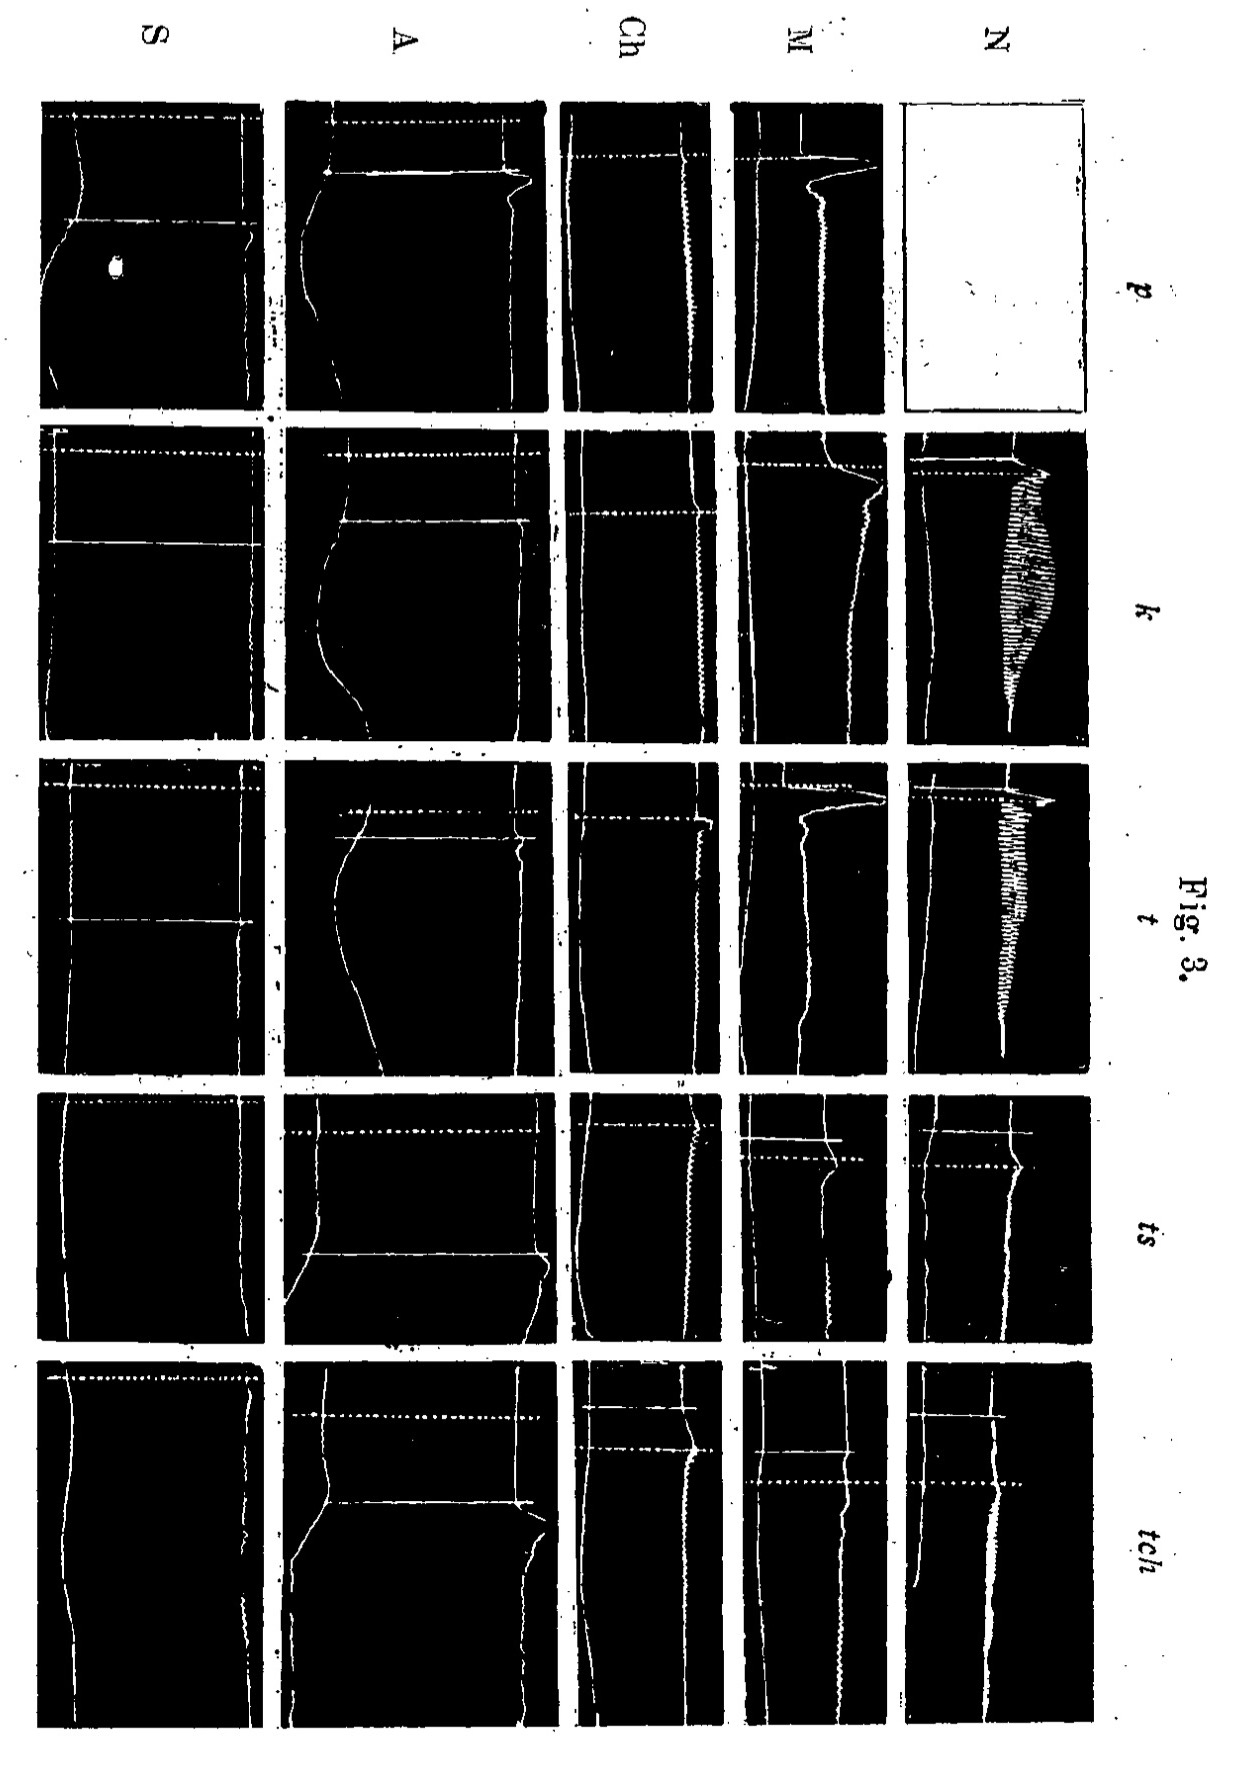
\includegraphics[scale= .3]{images/adjarian1899fig3.jpg}
}
	\caption{Original figure 3 for reflexes of Classical Armenian voiceless unaspirated stops and affricates}
	\label{fig:fig3 original}
\end{figure}


\begin{figure}
	\centering
	\resizebox{\textwidth}{!}{%
	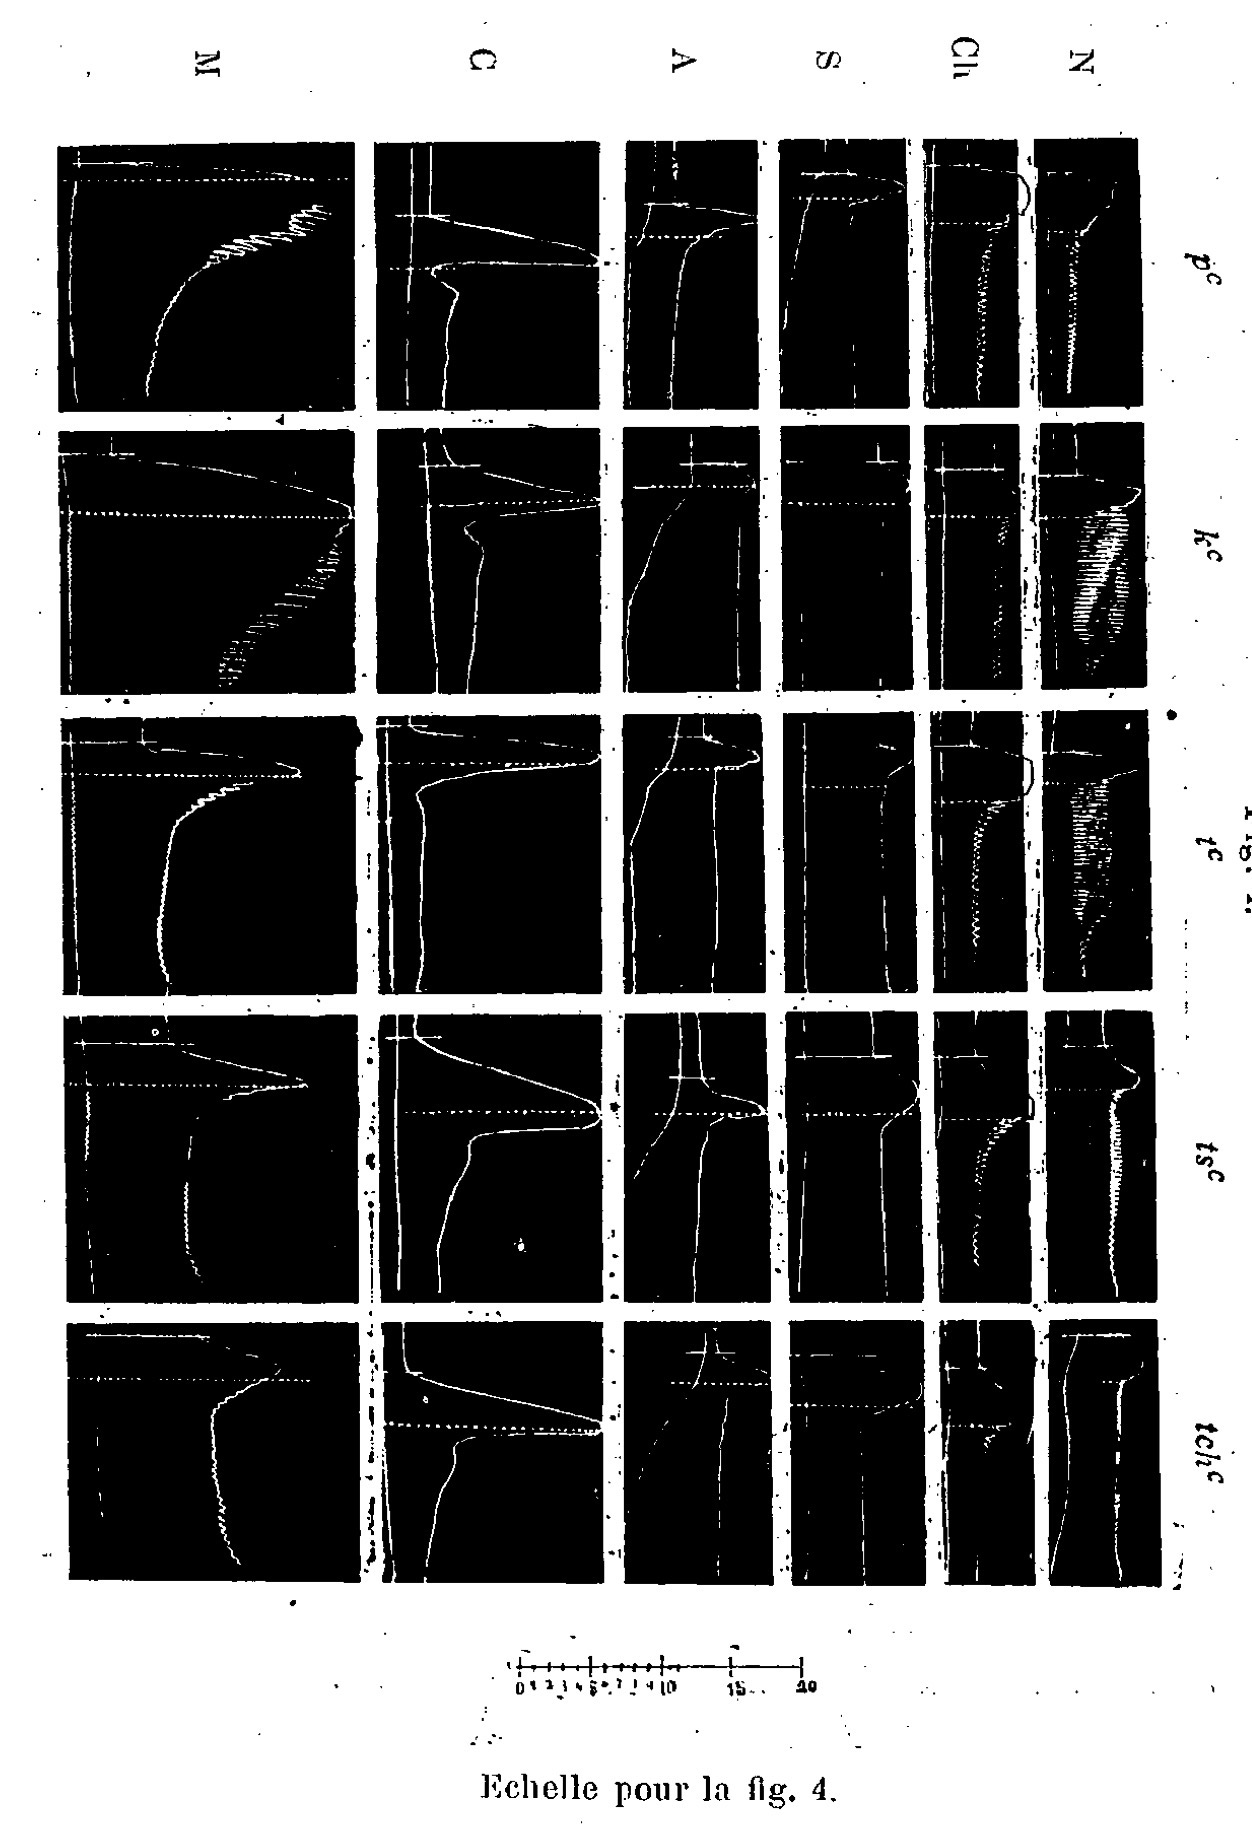
\includegraphics[scale= .3]{images/adjarian1899fig4.jpg}
}
	\caption{Original figure 4 for reflexes of Classical Armenian voiceless aspirated stops and affricates}
	\label{fig:fig4 original}
\end{figure}



One would be struck, I'm sure, by the amplitude of some of the vibrations, or the apparent weakness of some of the bursts. It's important not to dwell on this: it is all due, not to the phenomenon itself, but to the nature of the drum I have used.

To make it easier to compare my plots, I've grouped them in four tables, arranged so that the same articulation is read from top to bottom, and that the forms of the same dialect follow each other horizontally. When an articulation is missing in a dialect, the place it should occupy is left blank.

Two scales are used to measure the duration in hundredths of a second. The first, appended to Figure \ref{fig:fig1 original}, is used for tables 1, 2 and 3 ; the 2nd, for Figure \ref{fig:fig4 original}, to which it is attached.

The figures have been reproduced by photogravure. Some have been edited, but only for points that are outside the purpose of this work.

The experiments were carried out on the following people, each using the speech of his native town:

\begin{enumerate}
	\item First, myself, Hratchia Adjarian, born in 1874, in Constantinople (250,000 Armenians), for the popular and literary pronunciations.
	\item Mr. Alexandre Nalbandian, born in 1873, in Aslanbeg, a large Armenian village (4,000 inhabitants) near the town of İzmit (Ismidt), on the Sea of Marmara.
	
	\item Mr. Vahan Ter-Poghossian, born in 1872 in Nukha, on the southern side of the Caucasus, east of Tbilisi (Tiflis.
	
	\item The melik Nikoghos Avcharian, born in Shushi, in 1872.
	
	\item Mr. Tigran Dimaksian, born in 1878, in Karmen, an Armenian village near Mush.
	
	\item Mr. Georg Mkrtichian, born in Sivas in 1872.
	
\end{enumerate}


\section{The voiced stops and affricates of Classical Armenian}

\armenian{բ, գ, դ, ձ, ջ} – /b, ɡ, d,  d͡z,  d͡ʒ/ (Figures \ref{fig:fig1 original} and \ref{fig:fig2 original})... 

1. In the popular speech of Constantinople (C1, C2, C3), there are three ways of pronouncing these consonants: for the first manner, the laryngeal vibrations precede the air burst (by 0.08 seconds): for the second manner, the laryngeal vibrations occur at the same time as the air burst, and for the third manner, the vibrations occur slightly after the air burst (by only 0.01-0.02 seconds).

So, in reality, we have 3 varieties of voiced stops and affricates (3 \textit{b}, 3 \textit{ɡ}, 3 \textit{d}, etc.), but the third is far less distant from the second than this one is from the first.

The first, which corresponds exactly to French voiced consonants, is used when there is emphasis; it can therefore be called emphatic. The second, which corresponds to German voiced consonants, can be called normal, as the vast majority of examples belong to this type: such is the ordinary pronunciation of Constantinople. As for the third, I have only observed it accidentally. These voiced consonants are close to the corresponding voiceless ones, but they have less force, and the larynx enters into vibration faster than for the voiceless consonants.

2. In the literary language of Constantinople and in the dialect of Aslanbeg (A), voiced consonants are pronounced voiceless aspired consonants, which we'll discuss later (Figure \ref{fig:fig4 original} C, and A). However, in Aslanbeg, these consonants have less force than the corresponding aspirated ones (compare Figure \ref{fig:fig1 original}A and \ref{fig:fig4 original}A). Occasionally, they are pronounced like the voiced ones in the popular Constantinople speech (Figure \ref{fig:fig1 original} C1, C2, C3).

3. In the dialects of Nukha (N) and Shushi (Ch), they have remained completely voiced; vibrations of the larynx begin at variable times, up to more than 0.1 of a second before the air burst.

4. In the dialects of Mush (M1 M2) and Sivas (S), they have two distinct categories. The first (M1) presents voiced consonants in Nukha and Shushi. In the second (M2 and S), the consonant is pronounced more strongly than in the first, and the volume of air from the burst is more considerable,  which gives me the impression of a <bh> or a voiced [b] ([bʰ]) followed by a confused noise in the throat, whereas a French speaker hears [p].

The laryngeal vibrations begin 0.02-0.03 seconds after the air burst; but in two instances, for [b], there was simultaneity between the start of laryngeal vibrations and the air burst.

\section{The voiceless unaspirated stops and affricates of Classical Armenian}

\armenian{պ, կ, տ, ծ, ճ} – /p,  k,  t, t͡s,  t͡ʃ/
(Figure \ref{fig:fig3 original})

1. In the vernacular and literary languages of Constantinople, these consonants are considered voiced and are pronounced exactly like these (Figure \ref{fig:fig1 original} C1 C2 C3).

2. Similarly, in Aslanbeg and Sivas (A, S), they have become voiced: vibrations begin between 0.015 and 0.08 seconds before the air burst.

3. In the other dialects (N, M, Ch), they have remained voiceless, and perfectly distinct from both the corresponding voiced and voiceless aspirated consonants.

In Nukha (N) and Shushi (Ch), laryngeal vibrations begin at the moment when air emission is impeded, which corresponds to the fall of the plotline after the first moment of the air burst.

In Mush (M), laryngeal vibrations generally begin at the same time as the air burst. Nevertheless, my examples of [t͡s] and [t͡ʃ] show exactly the same position as in the pronunciation of Nukha and Shushi. I've also found the same for the consonant [t].

In Mush, unaspirated consonants can also become voiced as in the dialects of Constantinople, Sivas, and Aslanbeg.


\section{The  voiceless aspirated stops and affricates of Classical Armenian}

\armenian{փ, ք, թ, ց, չ} –  pʰ, kʰ, tʰ,  t͡sʰ,  t͡ʃʰ


In Constantinople, in the popular and literary pronunciations, these are divided into 3 classes. In the first, the vibrations of the larynx occur 0.01 second after the start of the air burst; this corresponds roughly to the strong French consonants (Figure \ref{fig:fig1 original} C3). In the second case, vibrations begin at the point where air emission is hindered, in other words, at the highest point of the plotline (Figure \ref{fig:fig4 original} C, except for [pʰ]). In the third case, vibrations occur after the movement of airflow, or very shortly before (Figure \ref{fig:fig4 original} C, [pʰ]). But the first and third classes are very rare; I have merely found them accidentally.

2. In Mush (M), the situation is similar to the second class described for Constantinople.

3. In the other dialects (N, Ch, S, A), these consonants are completely voiceless: vibrations only begin after the air burst is completed.
	
	


%\section{Introduction}


Armenian culture is no different from any other in being intimately intertwined with the linguistic intricacies of its language; if, indeed, we can refer to a single Armenian language.\footnote{This paper developed from a paper delivered at the ``Armenian Linguistics in a Modern Perspective'' workshop held at the University of Leiden on March 26, 2003. I have followed the transliteration and transcription conventions of the Adjarian translation. I use IPA for my own renderings from my fieldwork. Thanks to Rivka Hyland, Ollie Sayeed, and Paige Wallace for comments on earlier drafts of this text.} When studying the language, we have to deal (at least) with Standard Western Armenian (SWA), Standard Eastern Armenian (SEA), Classical Armenian, and Middle Armenian.  The Armenian language encompasses more than just these literary varieties, however.  In addition to a number of arguably distinct languages,\footnote{If we employ the working definition that two linguistic varieties are separate languages if they are not mutually intelligible. \todo{ref}} such as   Zok or /zokeɾen/ <\armenian{զոկերէն}> (the language of Agulis \todo{refs}),  /kʲeʁɑt͡sʰǝneɾen/ <\armenian{Գյեղացըներէն}> (the language of Zeytun \todo{refs}),  /kʰesbǝnuokʰ/ <\armenian{Քեսպընուոք}> (the language of Kesab \todo{refs}),\footnote{  Also called in different sources /kʰ(ɾ)isdinuokʰ/ `Christian language' (the same name used by speakers of Svedia/Musaler dialect), and in Roman-script contexts ``Kesbenok,  Kes(s)aberen, or Kesspeneuts.''} and Lomavren, the language of the Armenian gypsies, there are more than 120 distinct dialects of Armenian documented in the literature.  Like the micro-cultures they represent, each of these dialects has its own unique archaisms and innovations.  For a sense of how much these dialects can differ from one another, consider the translations in \todo{(1)} of \todo{Hovhannēs T‘umanean’s} story ``The Liar,''  drawn from three geographic extremes of the Armenian-speaking world: Köprücü (northeast Turkey), Stepanakert (Karabagh), and Qaladuran (northwest Syria).

\begin{exe}
\ex  ``The Liar'',  /sutɑsɑnǝ/ <\armenian{Սուտասանը}>
\begin{xlist}
	\ex English: \\
ONCE UPON A TIME there lived a king. This king announced throughout the land:  
``I shall give half my kingdom to the man who can tell a lie that I admit to be a lie.''  
A shepherd came and said, ``Long May Your Majesty Reign! My father had a cudgel which he used to reach out from here and stir the stars in the sky.  
``That’s possible,'' answered the King. ``My grandfather had a pipe. He used to put one end of it in his mouth and stretch the other up to the sun to light it.''  
The man went out scratching his head.  
A tailor came and said, ``I am sorry, O King, to have come so late. I had intended to come earlier. But there was a heavy storm yesterday, and lightning rent the sky. I’ve been patching it up.'' 
``Oh, very commendable,'' said the King, ``but you haven’t patched it very well, for it rained a little again this morning.
This man also went away empty-handed.  
A peasant came in with a bag on his shoulder. ``What do you want, my good man?'' asked the King. ``You owe me a bag of gold. I have come for it.'' ``A bag of gold!'' exclaimed the King astonished. ``That s a lie. I do not owe you anything.''  
``All right. It is a lie. Then give me half your kingdom.''
``No, no. You’re quite right. It’s not a lie,'' the king tried to correct himself.   
``So I am telling the truth. Then give me the bag of gold.''

\ex Version 1: Köprücü,\footnote{  Narrated by Temel in Watertown, MA in 1995.}  a Hamshen subdialect, /χɑpʰoʁe/ \\

ɡonːɑ ɡu t͡ʃʰɡonːɑ ɡu mekʰ kʰǝɹɑl me ɡonːɑ ɡu.  ɑs kʰǝɹɑ́les uúne milːetʰin ɑnons ɡenɑ:  ‘vov u ɔ́jle biɹ χɑpʰɑ́ɑnɑ jes ɑsim χɑpʰelu t͡ʃʰɑ, im kʰǝɹɑlːouz ɡɛ́se ɡɑɹnu.’  kʰu kʰɑ hojiv me ɡɑsɑ, ‘kʰǝɹɑ́le sɑʁ elːi, im bɑbɑs hɑst meɡ pʰiɹ me uneɹ, ɑn pʰíɹe isti eɹɡent͡sʰenelov hɑvɑjin ɑstɑʁníje χɑɹne ɡuɹ.’  ‘elːi ɡɑɑ,’ kʰǝɹɑ́le d͡ʒevɑb ɡu dɑ.  ‘im bɑbs ɑ mekʰ pʰipʰo me uneɹ meɡ d͡zɑ́ɹe pʰiɑ́ne tʰene ɡuɹ meɡ ɑl d͡zɑ́ɹe ɑɑkʰɑɡɑn kʰole ɡuɹ.’  χɑpʰɔ́ʁe kʰelɔ́χe kʰijelov heɹunɑ ɡu.  tʰeɹzi me kʰu kʰɑ ɡɑsɑ, ‘ɑf ɑɑ́, kʰǝɹɑl, tʰez me kʰɑ ɑmɑ uʃɑt͡sʰɑ. ejekʰ ʃɑtʰ t͡ʃʰɑχ ejev ʃimʃekʰnɛ́ɹe ɡɑd͡zɡedet͡sʰin hɑvɑn bɑdeɹet͡sʰɑv ɡɑɹɡɑuʃ kʰenɑɑd͡z e.’  ‘hɑ, bedkʰ e ɑʁɑ́d͡zues,’ kʰǝɹɑ́le ɡɑsɑ, ‘ɑmɑ soj ɡɑɹɡɛ́de t͡ʃʰɑɹt͡sʰɑd͡z es.  ɑsɑkʰvɑn ɑ kʰit͡ʃʰ me t͡ʃʰɑχ ejev.’ tʰeɹzin ɑ tʰus kʰelːɑ.  ɑχkʰɑd mɑɹtʰ me met͡ʃʰnuz mednu ɡu tʰevin dɑ́ɡe kʰovɑ me.  kʰǝɹɑ́le hɑɹt͡sʰenɑ ɡu, ‘tʰun int͡ʃʰ kʰuzes tʰɑ?’  ‘ind͡zi meɡ kʰovɑ me ɑltʰun dɑlikʰ unes; donuʃ eɡɑd͡z im.’  ʃɑʃiɹmiʃ ɡenɑ kʰǝɹɑ́le, ‘meɡ kʰovɑ me?  χɑpʰes ɡu, jes kʰezi ɑltʰun dɑlikʰ t͡ʃʰunim.’  ‘mɑdem kʰi χɑpʰi ɡum nɑ, kʰǝɹɑlːǝʁǝtʰ ɡɛ́se du.’  ‘t͡ʃʰɑ t͡ʃʰɑ, ʃidɑɡ χɑɹbe ɡus,’ kʰǝɹɑ́le ɑstɑ́d͡ze tʰɑɹt͡sʰenɑ ɡu. ‘ɑstɑ́d͡zes ʃidɑɡ ɑ tʰɑ ɑ nɑ, du kʰovɑ me ɑltʰúne.’  t͡ʃʰɑɹesiz kʰǝɹɑ́le kʰovɑ me ɑltʰúne ɡu dɑ.

\todo{mention ɹ in intro from bert's hamshen work}

\ex Version 2:  Stepanakert  (Karabakh),\footnote{Narrated by Vladimir in Cambridge, MA on September 10, 1995.} /sot \'ɑsoʁǝ/

inúm ɑ t͡ʃʰinúm min tʰɑkʰɑvɔ́ɾ ɑ inúm.  es tʰɑkʰɑvɔ́ɾǝ ýæn jeɾkɾúm tɑɾɑ́t͡sum ɑ:  ‘hu min sot ɑsí, veɾ jes ɑ́sim sot ɑ, im tʰǝkʰɑvoɾutʰjɑ́n kɛ́sǝ yɾɑ́n kǝtɑ́m.’  min t͡ʃʰóbɑn kʲɑm ɑ ɑsúm, ‘tʰɑkʰɑvɛ́ɾǝ ɑ́pɾɑt͡s kenɑ́.  im hæɾ min kɔ́pɑl ɑ ynet͡sʰɑl veɾ estɛ́ʁit͡sʰ mɛ́knum eɾ jeɾkinkʰi ɑstʁɛ́ɾneɾ χɑ́rnum.’  ‘kǝpǝtɑ́hi,’ tʰɑkʰɑvɛ́ɾǝ ɑsum ɑ.  ‘im pɑpn el min t͡ʃʰúbuχ ɔ́neɾ min t͡sɛ́ɾǝ piɾɑnín eɾ tinúm en min t͡seɾn eɾ mɛ́knum ɑ ɑɾevít͡sʰ vɑ́ɾum.’  sot ɑ́soʁǝ kǝlóχǝ kɔ́ɾelɑv tys æ kʰʲinum.  min dɛ́ɾd͡zɑk ɑ kʲɑm ɑ́sum, ‘neɾʁutʰjún tʰǝkʰɑ́veɾ, jes ɛ́kʰyt͡sʰ pɪti kʲǽi uʃɑt͡sʰɑ.  jeɾɛ́k ʃɑt tʰoɾ jekɑ́v.  kǝt͡síkǝɾɑknéɾǝ tǝɾɑket͡sʰín jɛ́ɾkinkʰǝ t͡ʃǝʁvɛ́l eɾ kʲet͡sʰɑl eí kǝɾkǝtɛ́lu.’  ‘hɑ, lɑv ǝs ǝɾɑ́l,’  ɑsum ɑ tʰǝkʰɑ́veɾǝ, ‘bɑjt͡sʰ lɑv t͡ʃʰǝs kǝɾkɑ́tɑl.  es ǝrɑ́vut el mi χǝɾɛ́ɡʲ ɑnd͡zɾɛ́v jɛ́kɑ.’  es el ɑ tys kʲinúm.  min kʰʲɑ́sib ʃinɑ́t͡sʰi ɑ ni mǝtnúm, kɔ́tǝ kúrnǝ tɑ́kin.  ‘tu hint͡ʃʰ ǝs ɔ́zum ɑj mɑɾtʰ?’ tʰǝkʰɑ́veɾ hɑɾt͡sʰnúm ɑ.  ‘ind͡z min kot vǝ́ski ǝs pɑtkʰ.  jɛ́kɑl ǝm tɑním.’  ‘mi kot vǝski?’  zǝɾmɑ́num ɑ tʰǝkʰɑ́veɾǝ, ‘sot ǝs ɑsúm.  jes kʰez vǝ́ski t͡ʃʰem pɑtkʰ.’  ‘devɛ́ɾ sot ǝm ɑsúm, tʰǝkʰɑvoɾutʰjɑ́nǝtʰ kesǝ ind͡z to.’  ‘t͡ʃʰe t͡ʃʰe, dyz ǝs ɑsúm,’ χɔ́skʰǝ pʰɔ́χum ɑ tʰǝkʰáveɾǝ.  ‘devɛ́ɾ dyz um ɑsum, mi kot vǝskis tuɾ.’

\ex Version 3:    Qɑlɑduɾɑn  (Kesab),\footnote{Narrated by Mr Manjikian in Watertown, MA in January 1995.} /sot χusuǝʁǝ/

ɡit͡sʰiɾ i t͡ʃʰi ɡit͡sʰiɾ i tʰækʰævyɾ mǝ.  æt tʰækʰævyɾǝ ɡesi eɾ ihɑlen:  ‘uv ǝɾ mit͡s seœd mǝ χysæ, is esim seœd i, tʰekʰevyɾytʰynes ɡesǝ ɡudum eɾ.’  ɡu kʰu huvev mǝ ɡesi, ‘tʰekʰevyɾǝ sɑʁ ɡinœ.  im dyǝdǝ ɡuniǝɾ huest veɾyt͡sʰ mǝ, zæn ɡidnæn ɡǝ minɡieɾ tǝɾviɾ zeɾɡinkʰen zɑɾɑstɑʁ ɡinːiɾǝ ɡǝ χeɾinɡeɾ.’  ‘ɡɑɾnu ǝnːu,’  ɡesi tʰekʰevyɾy, ‘im duedǝ ɡunieɾ qelun mǝ mieɡ d͡zɑɾkʰǝ biɾunǝ ɡǝ tǝniǝɾ miæl d͡zɑɾkʰǝ ɡǝɾɡent͡sʰǝniǝɾ eɾiven ɡǝ vɑɾieɾ zǝ.’  sot χusuǝʁǝ ɡǝ hɑɾvǝno kʰǝloχǝ kʰǝɾiluǝn.  ɡu kʰu tʰeɾzej mǝ, ɡesi, ‘neɾoʁutʰjun tʰekʰevyɾ, is evilæ uχtuǝv bidæ ukʰeɾem himit͡sʰæ iɾiekʰ ʃuǝt end͡zǝɾiv iɡikʰ.  ɡǝd͡zɡǝdilien ɡɑɾdilien eɾɡenkʰǝ bɑdǝɾit͡sʰuǝv ɡet͡sʰuǝd͡z eɾem zǝ ɡeɾɡedilǝ.’  ‘ʃuǝt æʁyɾ iɾuǝd͡z is,’ ɡesi tʰekʰevyɾǝ, ‘ǝmːǝ æʁyɾ t͡ʃʰi ɡeɾɡeduǝd͡z eɾe zǝ. æs sǝbæχtæn kʰejt͡ʃʰ mǝ end͡zǝɾiv iɡikʰ.’  tʰeɾzejn ili tuɾit͡sʰi ɡǝnːi.  nikʰsi ɡǝ mǝnːæ æχkuǝt keʁet͡sʰej mǝ ɡulued͡zǝ tʰiven duǝkʰǝ.  ‘teon t͡ʃʰej hæ uzis ɑj moɾtʰ?’ ɡǝ hɑɾt͡sʰǝni tʰekʰevyɾǝ.  ‘ǝnd͡zi mieɡ ɡuluǝk isɡæ buoɾdkʰ is.  iɡuǝd͡z im zǝ denilǝ.’  ‘ɡuluǝm isɡæ?’  ɡǝ ʃɑʃmǝʃǝnːo tʰekʰevyɾǝ, ‘seœd hæ χusejs.  is kʰi isɡæ buoɾdkʰ t͡ʃʰim.’  ‘æn kʰi seœd hæ χusejm, tʰekʰevuɾutʰunetʰ ɡiese deo.’  ‘t͡ʃʰi t͡ʃʰi, uʁuɾtʰ hæ χusejs,’ χueskʰǝ hæ pʰeχi tʰekʰevyɾǝ.  ‘tʰi uʁuɾtʰ i im esuǝd͡zǝ, deo ind͡zi ɡuluǝmǝ isɡæ.’  umodǝ ɡǝdǝɾiluǝn tʰekʰevyɾǝ ɡu dued͡zeɾ ɡuluǝmǝ isɡæ.
\end{xlist}
	\end{exe}

  
The study of Armenian dialects ties together the present and the past as well as many different disciplines -- linguistics, history, folklore, anthropology, and music -- and geographical areas as diverse as Syria, Abkhazia, Iran, and India. Yet the field faces three challenges: the tools and methods of the field are still situated firmly in the 19th century;\footnote{Bernard Coulie observed in his presentation at the ``Armenian Linguistics in a Modern Perspective'' conference, ``Language and Text: The Material Basis of Our Research of Classical Armenian'' (subsequently published as Coulie 2014) that the situation is similar in Armenian manuscript studies and chronology. }\todo{refs} like many academic pursuits, Armenian dialectology is under threat as a result of economic developments in post-Soviet Armenia and Karabagh; and most of the non-standard dialects of Armenian are in imminent danger of disappearing altogether. 


These are the problems I address in this chapter. After surveying the present and past of the field, which revolve primarily around the activities of Hratchia Adjarian, I suggest some ways in which Armenian dialectology can make use of advances that have been made in general dialectology since Adjarian’s time, and consider what steps can be taken to document and perhaps even stabilize or revitalize the dialects before it is too late.




\section{The state of Armenian vs. American dialectology}


The central concern of work to date on Armenian dialects by scholars in Armenia, as well as by the majority of more recent Western scholars such as Andrzej Pisowicz and Georges Dumézil, has been the collection of word lists and short texts and the evaluation of their etymological significance relative to Classical Armenian. The manual for collection of Armenian dialect materials published by the Dialectological Institute (Muradyan et al. 1977 \todo{ref}) and the Institute’s activities since that time indicate that it intends to continue this course of action. 	

Such work is valuable and provides the groundwork for a wide range of illuminating research. However, the methodology employed by Muradyan et al. directly reflects the state of European linguistics and dialectology in the late nineteenth century, when the leading Armenian linguist, Hratchia Adjarian, studied in Paris under the Indo-Europeanist Antoine Meillet. Many important developments in linguistics and dialectology have occurred since that time, particularly due to the theoretical linguistic work of Noam Chomsky beginning in the 1950s and the sociolinguistic work of William Labov beginning in the 1960s. Since the appearance of the new concepts and methodologies developed by these scholars, linguistics and dialectology have advanced at great speed; it seems only logical, then, that dialectologists working on Armenian should benefit from these new methods. 	

The need for more comprehensive and contemporary methods of investigation is particularly imperative given the impending extinction of many (and perhaps most) of the remaining non-standard Armenian dialects. Soon it will no longer be possible to compensate for omissions in the work of earlier researchers by consulting native dialect speakers. In the remainder of this section I sketch the history of traditional work on Armenian dialects, contrast this with developments in Western dialectology in the twentieth century, and suggest some ways in which incorporation of the latter can enhance the former.


\subsection{Armenian dialectology}
	
\subsubsection{The past}
	
\subsubsubsection{Proto-dialectology}

\todo{paragraph?}

In a sense, the first known Armenian dialectologist was \todo{name}Mesrob’s student Koriwn\todo{name}. In his fifth-century biography of Mesrob, Koriwn mentions the existence of Armenian dialects in Siwnik‘\todo{name} and the land of the Medes (i.e. Agulis in this context). The fifth-century theologian \todo{name}Eznik\footnote{cf. Blanchard and Young 1998 for an English translation of Eznik’s text. \todo{ref}} observed  in turn that in his time there were two dialects of Armenian: one in the north and one in the south. Speaking of the Classical Armenian form /ɑi̯s/ <\armenian{այս}>, he says:

\begin{exe}
	\ex Classical Armenian \\
	\gll  Յորժամ մեք ասեմք թե սիք շնչե, ստորնեայք ասեն` այս շնչե \todo{check spelling} \\
	yoržam mek‘ asemk‘ t‘e sik‘ šnč‘e, storneayk‘ asen` ays šnč‘e	
	‘when we (i.e. Armenians of Koghb and northern Armenia) say sik‘ šnč‘e [for ‘a wind is blowing’], the southern [Armenians] say ays šnč‘e.’ \todo{fix all this}
	
\end{exe}


The form   /ɑi̯s/ <\armenian{այս}>  was in fact used in the north, but in the meaning `evil spirit' or `demon'; the southern Armenians preferred   /deu̯/ <\armenian{դեւ}>  for this function.	

Armenian dialects are next mentioned by the early Armenian grammarians; the sixth century translation of Dionysus Thrax refers to the dialect of \todo{Gordayk‘}, for example, and the eighth century commentary of \todo{Step‘anos of Siwnik‘} mentions eight dialects: \todo{Korchayk‘, Tayk‘, Khut‘ayk‘, Fourth Armenia, Sperk‘, Siwnik‘, Arts‘akh, and Central Armenia (Ararat).}


A significant amount of subsequent work, notably by Weitenberg and Jahukyan, has been devoted to identifying the nature and extent of dialect variation in the Classical Armenian period; this will be addressed in sections \todo{2.1.1.4 and 2.1.2.}

\subsubsubsection{The beginnings of Armenian dialectology: the 18th century}

\todo{paragraph?}

The first published analysis of significant amounts of Armenian dialect material was \todo{Rivola's} (1633) \textit{Dictionarium Armeno-Latinum}, which contained numerous lexical items from New Julfa and other dialects. Rivola did not distinguish between the dialects he employed, however, as \todo{Adjarian (1940)} points out.	

\todo{Schrœder's} \textit{Thesaurus Linguae Armenicae}, published in Amsterdam in 1711, provides extensive samples of Agulis, New Julfa, and other Armenian dialects, and documents contrasts between Civil Armenian (a form of proto-Modern Armenian; cf. \todo{Parnassian 1985}) and the classical language. 


\subsubsubsection{The heyday of Armenian dialectology: the nineteenth century}
	

\todo{paragraph?}

The nineteenth century saw an explosion of interest in the dialects of Armenian. \todo{Chahan Cirbied} (\armenian{Շահան Ջրպետեան}), a Tokat Armenian who early in his career taught a young \todo{Sunduk‘ean} in Tblisi/Tiflis and later was professor of Armenian in Paris, devoted an entire section of his \todo{1823} \textit{Grammaire de la Langue Arménienne} to some thirty nonliterary dialects of Armenian. Like Rivola, though, he generally does not specify the dialect from which he takes the individual forms he cites. In 1850, \todo{Shirmazanean} published his \textit{Patmut‘iwnk‘ i Lezu Erewanc‘oc‘} `Stories in the Language of the Yerevantsis,'  which discussed general features of the Yerevan dialect. In 1852, \todo{Hakhverdean’s Sayat‘-Nova} appeared in Moscow; the first portion of this landmark publication was devoted to the grammar of \todo{Hakhverdean and Sayat‘-Nova’s} native dialect of Tblisi. \todo{Aytĕnean’s} important \textit{K‘nnakan k‘erakanut‘iwn ashkharhabar kam ardi hayerēn lezui} [Critical Grammar of the Modern Armenian Language] appeared in Vienna in 1866. \todo{Aytĕnean} postulated the existence of Armenian dialects already in the fifth century, based on \todo{Koriwn’s} aforementioned reference to Armenian dialects in \todo{Siwnik‘} and the land of the Medes. He divided the modern dialects into four groups: Eastern Turkey, Western Turkey, Europe, and Russia/Persia/India. Petermann’s study of the Agulis dialect appeared in Berlin in the same year.	

Spurred on in part by the nationalism and romanticism sweeping through Europe, Armenian dialectology reached its zenith in the second half of the nineteenth century. Just as the brothers Grimm scoured the 19th-century German countryside in search of pure and ancient Germanic folklore, Armenians such as \todo{Garegin Sruandzteants‘} returned to their village roots in search of an epic narrative that could rival those being produced in neighboring countries. The discovery by \todo{Sruandzteants‘} of the Sasun epic (cf. his \textit{Mananay}, \todo{1876}) is one of the many fruits of this halcyon period of intellectual curiosity. Numerous works on the language and ethnography of Armenian villages followed in quick succession, documented in books such as \todo{Sedrakean’s} \textit{K‘nar Mshets‘wots‘ ew Vanets‘wots‘} (1874), \todo{Allahvertean’s} \textit{Ulnia kam Zēyt‘un} (1884), \todo{Sherents‘’s} \textit{Vana Saz} (1885, 1899), \todo{Haykuni’s} \textit{Ēminean Azgakrakan Zhoghovatsu} (1900-13), and \todo{Lalayean’s} \textit{Vaspurakan} (1914), and in journals such as \todo{Murch, Biwrakn, and Azgagrakan Handēs}.


The first Armenian dialectologist in the modern sense was \todo{Kerovbe Patkanov/Patkanean}, whose \todo{Izsledovanie o Dialektax’ Armjanskago Jazyka} [Treatise on the Dialects of the Armenian Language] appeared in Saint Petersburg in 1869. His monograph provided phonological and morphological sketches of the dialects of \todo{Astrakhan,} Yerevan, Tbilisi, Agulis, Karabakh, Khoy, New Julfa, Mush, Poland, and New Nakhichevan.\footnote{\todo{cit}He also produced longer separate treatments of the dialects of Agulis (1866) and New Nakhichevan and Mush (1875).} Soon thereafter, a veritable flood of dialect grammars began to pour out of Europe and Armenia; notable examples include \todo{Petermann’s} 1867 grammar of the Tblisi dialect, \todo{Sargseants‘’s} 1883 grammar of the Agulis dialect, \todo{Hanusz’s} 1886 dictionary and 1889 grammar of Polish Armenian, \todo{Tomson’s grammars of the Akhalts‘kha and Tbilisi} dialects (1887, 1890), \todo{Msereants‘’s} various works dealing with the Mush dialect (1897), and \todo{Gazanchean’s} monograph on the Tokat dialect (1899).


The high point of this period (and of all periods of Armenian dialectology) was the work of Adjarian, who studied with the French Indo-Europeanist Antoine Meillet in the 1890s, and was probably responsible for Meillet’s deep interest in Armenian. Adjarian was the first scholar to bring contemporary European linguistic tools to bear on the manifold intricacies of the Armenian dialects. Conversely, he made use of Armenian dialect materials to develop a phonetic concept that has occupied a central place in the Western study of phonetics since the 1960s, Voice Onset Time \todo{(Braun 2013; cf. Lisker and Abramson 1964)}. Adjarian was also unusually productive. Not only did he produce dozens of groundbreaking books on Armenian dialects and on the Armenian language in general; Adjarian also single-handedly founded the modern schools of Armenian linguistics and dialectology that still survive in Armenia today.

Adjarian established a method for collecting, presenting, and analysing linguistic materials that drew directly on Western linguistic work of the time. Though the work of the structuralists, Chomskyans, and variationists replaced it in the West in the twentieth century, armenologists today continue for the most part to use Adjarian’s method, particularly in Armenia. At the time Adjarian was learning linguistics in Paris in the late nineteenth century, European linguists were primarily interested in using linguistic data for historical purposes, especially the reconstruction of earlier stages of the language or language family under consideration. Dialect variation was understood to play a central role in this quest, insofar as it presented material for classification and subgrouping, thereby enabling triangulation to earlier historical stages, and as it contained archaisms that directly revealed aspects of the past, untainted (it was thought) by the vagaries of the modern world and literary languages. Because of this focus on historical questions in his intellectual milieu, Adjarian’s model for presenting dialect material revolved around the comparison of dialect forms to their antecedents in Classical Armenian, as shown in this sample from his grammar of the New Julfa dialect:

\begin{exe}
	\todo{fix}
	(3) 	§9 from Adjarian 1940 
	“Classical Armenian a normally remains a in all positions in the New Julfa dialect, e.g. ալիւր aliwr > ɑluɾ [flour], աղուէս aɫuēs > ɑʁvɛs [fox], առնել aṙnel > ɑniɛl [do], ասեղն aseɫn > ɑsuʁ [needle], աղանձ aɫanj > ɑʁɑndz [roast (n)], բարակ barak > bhɑɾɑk [thin], բարձր barjr > bhɑntshəɾ [high], բահ bah > bhɑχ [spade], ծիրան ciran > tsiɾɑn [apricot].”
	
\end{exe}

In order to facilitate comparisons of this type, and to make them consistent across dialects, Adjarian constructed a fixed word list that he employed for all of his field work and resultant dialect grammars. He would then extract a basic set of historical phonetic and morphological changes from this word list, append a few dialect texts with a handful of grammatical and lexical notes, and add an introduction briefly discussing the previous literature that he was able to find on and in the dialect. As was the case with his European teachers and colleagues, Adjarian was not overly concerned with identifying what individuals or texts each of his forms came from, nor did he consider the significant range of subdialectal and idiolectal variation that one finds in every dialect. For Adjarian, as for his contemporaries, dialects were for the most part idealized monoliths consisting of forms produced by older speakers that conformed to his historical expectations.


Linguistic work at the time also tended to neglect synchronic analysis of the grammatical system of the dialect at that point in time, and largely ignored acoustic phonetics, phonology (synchronic rules, rather than historical changes), syntax, and sociolinguistic nuances. The model that Adjarian developed for collecting and analysing Armenian dialect material was no exception to this. (\todo{Samvel Antʻosyan}, for example, divides his 1961 treatment of the Kayseri dialect into four sections: [historical] phonology, morphology, lexicon, and text samples.) Adjarian’s methods, as still practiced in Armenia today, provide an interesting window into the state of linguistic and dialectological research in Europe in the late nineteenth century.

\subsubsubsection{The fall of Armenian dialects and dialectology: the 20th century}
\todo{paragraph}

At the beginning of the twentieth century, Armenian dialectology was still at its peak. Meillet’s students Adjarian, \todo{Dawit‘ Bēk, Maxudianz,} and Benveniste produced an abundance of excellent dialectological studies. The school that Adjarian began in Armenia would ultimately generate such productive dialectologists as \todo{Jahukyan, Gharibyan, Grigoryan, the two Muradyans, and Adjarian’s niece, Amalya Khatchatrian.}


Despite the widespread interest in Armenian dialectology and folklore at the turn of the century, there were far more Armenian villages, dialects, songs, stories, and so on than could be collected by the army of amateur and professional armenologists. This was less true after 1915, when the Armenian populations of most of these villages were eradicated. Dialectological work has continued since 1915, with notable products such as \todo{Malkhaseants‘’s Hayeren Bats‘adrakan Baṛaran} (1944), the dialect grammars and dialect survey produced by the Institute of Dialectology in Yerevan (most notably Adjarian’s \todo{1954} treatment of the Van dialect and \todo{Davt‘yan’s 1966 atlas of Karabagh dialects}), \todo{Dumézil’s} studies of the Hamshen and Musaler dialects, \todo{Pisowicz’ grammar of the P‘arpi} dialect, and the memorial volumes produced by the various compatriotic organizations in the United States (e.g. \todo{Galustean 1934} for Marash). Popular interest in the language and culture of village Armenia has waned, though, a fact reflected in the evanescence of almost all of the compatriotic societies.

\subsubsection{The present}

At the present time, little is being published on Armenian dialectology. The Institute of Dialectology in Yerevan is still technically active, and engaged in the collection of materials for its dialect atlas. In practice, however, these plans appear to have been put on hold indefinitely, as Armenia and Karabkgh have been attending to more pressing matters. (One notable exception is Armen Sargsyan at Karabagh State University, who as of my visit in 2001 was still actively collecting dialect materials from Karabakh villages via his students from those villages.)

The bright light of current Armenian dialectology was until 2012 the University of Leiden in the Netherlands, which for some time featured three talented Armenian dialectologists, Jos Weitenberg, Uwe Blaesing, and Hrach Martirosyan. Weitenberg was primarily concerned with reconstructing the chronology of linguistic developments between Proto- and Modern Armenian, using evidence from manuscript `errors' and variation within the classical and medieval languages and the modern dialects. Of particular interest is his 2001 analysis of the chronological development of penultimate and final stress in the Armenian world, using sophisticated arguments from relative chronology. Blaesing is a turkologist by trade, but his wife is a Hemşinli, and he has consequently done a great deal of useful work on the Armenian lexical material that survives in the Turkish dialect of the Hemşin region of northeastern Turkey.

Weitenberg initiated in the 1990s a collaborative effort with the Dialect Institute in Yerevan, designed to facilitate the generation of isogloss maps from data collected via the \todo{1977} Muradyan manual from approximately 500 village varieties of Armenian. It remains to be seen whether the Institute’s database chronicles actual usage or a historical dialectologist’s conception of what a ``pure'' form of the dialect should have looked like at some point in the past, but in either case the maps resulting from this project should be quite helpful. We will turn to the challenge of constructing proper dialect maps in section \todo{3.}


\subsubsection{The future: the state of the Armenian dialects}

Many dialects, such as \todo{Nicomedia, Kirzan, and Shamakhi,} appear to be already dead; many more are alive but have only a handful of speakers remaining, such as Marash, Urfa, and Van. Zok, the Armenian dialect of Agulis, appears to have no more than two remaining speakers; Jerusalem lost its last fluent speaker less than twenty years ago. A fair number of dialects still have communities in which everyone speaks the dialect, but in some of these, such as \todo{Zeytun and Kesab,} the communities do not have a permanent location and will likely disappear in the near future. Those which do have permanent locations, such as Hamshen, \todo{Anjar, Diarbekir,} and the various dialects in Armenia proper and Karabakh (and perhaps \todo{Javakhk‘ and Abkhazia}), stand a better chance of surviving but are already beset by the pressures of the official languages of the countries in which they are spoken.

The key to understanding the future of these dialects is to look not at the number of people who speak them, but rather at the number of children who are learning them. Thus, for example, the number of Zeytun speakers is fairly large, but of the Zeytuntsis I worked with in Boston from 1990-2003 none had children who speak the dialect. By this measure, in fact, even SWA is in trouble. To the best of my knowledge, the only forms of Modern Armenian that are relatively secure for the immediate future are Eastern Armenian and Iranian Armenian.

Another problem is that many (and perhaps most) of the surviving dialects have yet to receive proper study. This includes many dialects in Iran (\todo{Tabriz, Chaharmahal, and many smaller villages, as well as the regional standard of Teheran), Iraq (Baghdad, Basra, Mosul, and the northern villages such as Zakho and Tell Kibār} that were inhabited by Armenians until the American invasion in 2003), \todo{Nakhichevan (speakers of several of these dialects currently reside in the south of Armenia), Jerusalem, western Turkey (Bolu , Smyrna, Adapazar, etc.}, and even Ethiopia and Turkmenistan. (It is not clear that the latter two Armenian communities actually possess distinctive dialects, as they have not been closely studied.) The mixed language of the Boshas, Lomavren, whose grammar is taken from the \todo{Erzerum} dialect of Armenian, also remains to receive extensive systematic study.

\subsection{Documentation}
Although a good deal remains to be done in the documentation of Armenian dialects, much work exists in both published and unpublished form. In this section I survey some of the more important work carried out to date, and compare the state of publication on Armenian dialects to that of English dialects.

\subsubsection{ Documentation of Armenian dialects}

\subsubsubsection{Syntheses}

A number of synthetic works on Armenian dialects and Armenian dialectology have appeared to date, most notably the aforementioned \todo{1869 monograph by Patkanov}, Adjarian’s doctoral thesis (published in French in \todo{1909 and in slightly expanded form in Armenian in 1911}), \todo{Gharibyan 1953 and 1958, Grigoryan 1957, Jahukyan 1972, Asatryan 1985, and Greppin and Khatchatrian 1986}. The last of these merely summarizes briefly the phonological rudiments of a few of the better-known dialects, but has the advantage of being the only description available in English (though the text samples for each dialect are not translated). Adjarian \todo{1909} is older, but is significantly more comprehensive and should be preferred by those who are unable to read Armenian. \todo{Adjarian’s \textit{Complete Grammar of the Armenian Language} (1952-1971)} contains a wealth of dialect information, but this material is not systematically presented, being interspersed sporadically throughout all seven volumes, and therefore is not as useful as most of the other synthetic works.

\todo{Jahukyan 1972} differs from the other works just mentioned in that it does not contain actual descriptions of dialects or even scattered dialect expressions or words, but instead contains a wealth of phonological, morphological, geographical, and bibliographical information on 124 different varieties of modern, medieval, and ancient Armenian. It moreover contains an enormous and unparalleled bibliography of books, articles, and unpublished manuscripts dealing with Armenian dialects, most of which are almost impossible to procure outside of Yerevan.  I have found this to be the dialectological treatise that I most often consult. The analytical component of the book, however, is somewhat problematic, as I discuss in section \todo{2.3.1.2.}

The above-mentioned studies are most useful and reliable in the sense that they were produced by linguists, but naturally suffer from their age, which prevents them from incorporating the host of more recent documentation, such as \todo{Kostandyan 1979 (Kharberd-Erznka), Lusents‘ 1982 (Aresh), Muradyan 1982 (Moks), Haneyan 1982 (Edesia), Madat‘yan 1985 (Alashkert), Ch‘olak‘ean 1986 (Kesab), Hapēshean 1986 (Musadagh), Markosyan 1989 (Ararat), Mezhunts‘ 1989 (Shamshadin-Dilijan), Hananyan 1995 (Khdrbek), and Adjarian 2003 (Cilicia; written much earlier, but unavailable until his manuscript was finally published in Yerevan in 2003}). Jahukyan makes use of these more recent works in his \todo{1997} monograph on dialectal elements in Armenian colophons, but the scope of this work is greatly restricted compared to that of the synthetic works discussed above.

Though they are synthetic in a larger but not dialectological sense, one should include here the \todo{Soviet Armenian Encyclopedia (Hambarts‘umian et al. 1974-1986), Petrosyan et al. 1975, and Petrosyan 1987}, which have brief but useful entries for dozens of dialects, including many whose grammars are not readily available outside of Yerevan.

\subsubsubsection{Non-linguistic collections}

Armenia has also produced a wealth of non-linguistic materials that happen to be of great use for dialectological purposes, though their transcriptions are often unreliable, omitting phonetic nuances in order to increase readability and/or because the transcriber, not being a linguist, did not notice them. Still, these collections can be useful for morphological, syntactic, lexicographic, and sometimes even phonological purposes. An incredible resource that remains largely untapped by dialectologists is the folklore collections \todo{(Tēr Aghēk‘sandrean 1886, Lalayean 1892, 1899, 1901, 1914, Haykuni 1900-1913, Abeghyan 1944-, Malkhaseantsʻ 1958, Orbeli et al. 1959-, Aṛak‘elyan 1970-, Grigoryan-Spandaryan 1971, etc.),} which in most cases have the advantage of providing the name, age, and specific village of origin for each storyteller. The various ethnographic works by \todo{Sruandzteantsʻ (Mananay (1876), T‘oros Aghbar (1884), Hamov Hotov (1884))} also contain many dialect texts, though their exact provenance is not always as thoroughly detailed as in the other works. The journal \todo{Biwrakn}, produced in Constantinople at the turn of the twentieth century, features dozens of dialect texts lacking the same sorts of information as those published by \todo{Sruandzteantsʻ}. Since virtually none of these sources  provide translations of their dialect texts into a western language or even into Standard Armenian, it is also appropriate to mention here \todo{Charles Dowsett’s} \textit{Armenian folk-tales and fables}, published in 1972 under the pseudonym of Charles Downing. The book contains 63 folk tales and fables, as well as ten pages of proverbs, translated from a wide range of Armenian dialects into English. The source for each story is clearly documented, so that one can easily track down the original Armenian (or Russian) versions.

Primary literary sources written in non-standard dialects also contain a wealth of dialect material, such as for the Tblisi dialect \todo{Sayatʻ-Nova (Hakhverdean 1852) and Sundukyan (1863 et seqq.; see his collected works, 1951-1961), Shirvanzade in Shamakhi dialect (1885, 1905, 1911, 1920, etc.; see his collected works, 1958-1962), Zargarean in Agulis dialect (1912), Ayvaz in Istanbul dialect (2001), and so on.}

Certain collections of riddles, sayings, games, and other ethnographic materials are also rich sources of dialect, notably \todo{Abeghyan’s collection of games (1940), Ghanalanyan’s collection of sayings (1960), Harutʻyunyan’s collection of riddles (1965), and Sargsyan’s collection of riddles from Karabagh (2002).} Though the dialect materials contained in these books are almost all taken from previously published sources, they remain valuable thanks to their thematic organization and the fact that many of their sources are not available outside of Yerevan. One problem with these collections is that when a given saying, riddle, etc. occurs in several dialects, they only provide a single, somewhat standardized rendition of it, leaving out information about the particular form it takes in any of the individual dialects. For instance, \todo{Harutʻyunyan 1965 states that riddle #951b (Q. ɛɾku ɔtʰɑʁ, min sjunɑni ‘two rooms, one pillar’; A: kʰitʰ ‘nose’) is used in Karabagh, Nakhichevan, and Borchʻalu,} but does not say which of these dialects (if any) the particular pronunciation he employs is from. \todo{Sargsyan 2002} has a more serious version of the same problem; whereas in many cases one can recover the original sources (and hence the informants) from \todo{Harutʻyunyan’s work}, because he provides references for his riddles, Sargsyan’s riddles are taken directly from uncredited native speakers, and it is therefore impossible to know exactly where they are from. This is an important lacuna in a work on Karabakh, since the region contains numerous distinct dialect groups \todo{(q.v. Davtʻyan 1966).} Sargsyan (personal communication) states that his informants are from \todo{Martuni and Hadrutʻ}, but this is still not sufficient information to place his rich materials in their proper dialectological context.

\subsubsubsection{Dictionaries}

We have a number of excellent dialect dictionaries, each of which possesses certain drawbacks. \todo{Adjarian 1913} features several thousand words and expressions, each of which is identified by its dialect of origin, but he regularizes their phonology, merges many dialects, and lacks data for the numerous dialects studied after the publication of his book. \todo{Amatuni 1912} has a host of data not to be found elsewhere and covers many dialects, but Amatuni was not a linguist and hence his renditions of the forms are unreliable. Also, like \todo{Achaṛean 1913,} he does not include many dialects and merges forms for disparate dialects. 

\todo{Achaṛean’s Armenian etymological dictionary} (published in handwritten form in \todo{1926, and then in typeset form in 1971-1979)} is for most purposes the most useful dialectal (and historical) dictionary, because it provides fairly reliable transcriptions and is organized by Classical Armenian headword, so it is relatively easy to compare forms in different dialects. However, an inevitable consequence of its early publication date is that many dialects are not included. In addition, often the Classical headword for a given dialect form is not obvious, and words not derived from classical forms are missing. Moreover, non-etymologically related words are not included in a given entry; for instance, the entry for Classical eɾ \todo{‘why’ (originally the genitive singular form of i ‘thing, what’)} provides the dialectal forms \todo{Davrēzh heɾ, Maragha heɾ ~ hejɾ, and Astrakhan neɾ (volume 2, p. 119)}, but does not mention other common dialectal forms for \todo{ ‘why’, such as intʃʰu, uɾ, əndeɾ, χi, χɑ, χɑs, hɔɾi, him, and zme (cf. Suk‘iasyan 1967:234). Only in the entry for intʃʰ ‘what’ (volume 2, p. 245) does one find mention of parallel forms intʃʰu, New Julfa tʃʰum(ɑɾ), Alashkert ɦəntʃʰi, and (in unspecified dialects) əntʃʰu, intʃʰi, and hintʃʰi embedded in Adjarian’s discussion of derivatives of intʃʰ.}


The excellent four-volume explanatory dictionary of Modern Armenian published by \todo{Stepʻan Malkhasyantsʻ in 1944} is replete with dialectal and other forms not found in conventional dictionaries, and is what I most often use when parsing both standard and dialect texts. However, \todo{Malkhasyantsʻ} does not cite the dialects or sources from which he takes each entry, and he conveys few nuances of non-standard pronunciation; his work is therefore more consistently useful for translation than it is for dialectological analysis.

\todo{Sukʻiasyan’s 1965} synonym dictionary is useful for identifying dialect variants, as shown by the entries for \todo{gɑzɑɾ ‘carrot’ (p. 133) and həndkɑhɑv ‘turkey’ (p. 393) in (4) and (5) respectively:}

\begin{exe}
	\todo{ref}
	(4)	gɑzɑɾ, g[ɔjɑkɑn ‘noun’]. 1. stɛpʁin: 2. stɛpʁin vɑjɾi, dɔks, tʃɑnduk, ɑʃmunisɑ, kʰɛʃiɾ:
	
	(5)	hndkɑhɑv, g[ɔjɑkɑn ‘noun’]. (kend[ɑ]b[ɑnɑkɑn ‘zoological].) hnduhɑv, hndkɑkʰɑʁɑʁ, (b[ɑ]ɾb[ɑɾɑjin ‘dialectal’].) tʃuɾtʃuɾ, tʃuɾtʃuɾ, gɔɾɛl, kɔɾɛl, tʃɔlɔk, kulkul, kuɾkuɾ, msɾɑhɑv, kʰɛlkʰɛl, tʃuluχ.
	
\end{exe}

Like \todo{Malkhasyantsʻ 1944, though, Sukʻiasyan} does not provide references for specific forms. One cannot infer from his book, for example, that \todo{չուլուխ tʃʰuluχ is used for ‘turkey’ in Hamshen (Acharean 1947:262; cf. Turkish çulluk ‘woodcock’ (Scolopax rusticola)), or even that ստեբղին əsdɛpʰʁin is the form for ‘carrot’ in SWA}. Key variants moreover are not included, such as the `turkey' form hindig in Abkhazian Hamshen (Avik Topchyan, personal communication), or the `carrot' forms\todo{ Baberd pʰəɾtʃʰulig, Tomarza pʰyrtʃʰykʰly, Gyumri pʰuɾtʃʰuluʁ, Kharberd and Kesab pʰɾtʃʰækʰli (for all of these cf. Turkish dialectal purçuluk), and Marash hɑvutʃʰ ~ havundʒ (cf. Turkish havuç). Oddly, Sukʻiasyan’s entry for the regional ‘carrot’ variant stepʁin (related to Greek staphulinos) includes forms not mentioned in the entry for gɑzɑɾ: tɑpʁin (which is used in Van, though Sukʻiasyan does not mention this) and teʁpind.}

\todo{Artem Sargsyan} and his team in Yerevan completed their seven-volume \textit{Dialect Dictionary of the Armenian Language} in 2012, but it is missing key requirements for a modern scholarly tool. It has the advantage of covering many more dialects than the other sources mentioned above, but is surprisingly limited in its coverage given the resources available in Yerevan; most of the dialect forms that I have looked for in it have not been there, and well-known dialects such as the Muslim Hamshen varieties described by \todo{Dumézil (1963 et seqq.)} are not incorporated. One also finds curious omissions of well-known dialect forms; for example, \todo{New Julfa լապստակ lɑpstɑk is missing from the entry for ‘hare’}. This same entry reveals another problem: it is unclear why the authors have separated from one another variant forms within a single dialect, e.g. \todo{լափստրայ lɑpʰstrɑj and լափստրակ lɑpʰstrɑk for Urmia.}

Along similar lines, when there is more than one reference for a specific dialect in an entry, the authors do not make clear which one a given form is taken from, nor where in the source text to find it. The citation of variant forms is inconsistent, as well; for instance, the entry for \todo{esōr} cites the variant form \todo{əsōr, but not the variant sōr.} The entry for \todo{էր ɛɾ ‘why’ (volume 2, p. 32)} mentions that it is used in Ararat, but does not provide a link to the aforementioned related forms \todo{Tabriz հէր hɛɾ, Maragha հէր hɛɾ ~ հէյր hɛjɾ, and Astrakhan նէր nɛɾ cited by Acharean} in his etymological dictionary.

The dictionary also is often not specific about dialect forms and references, as can be seen in the following example:

\begin{exe}
	\todo{f}
	
	(6) 	sample entry from Sargsyan et al. volume 2, p. 30
	ԷՍՏՈՒՐ, Ար. Ն. ԸՍՏՈՒՐ, Ղրբ. Սրա: Էստուր համար եմ ասում, որ լավ տղա է (ՎՏՍ): Փուղ պիտի վուր էստուրը դիմանա (ԳՍ): Ըստուր յաղի մին:
	
	ɛstuɾ, Ar. N əstuɾ, Ghrb. Sra. ɛstuɾ hɑmɑɾ ɛm ɑsum, vɔɾ lɑv tʁɑ ɛ (VTS). pʰuʁ piti vuɾ ɛstuɾə dimɑnɑ (GS). əstuɾ jɑʁi min.
	
\end{exe}

This entry provides no sources for the \todo{Ar [Ararat], N [Nakhichevan?], and Ghrb [Karabagh]} forms, nor does it give precise references that would enable one to locate the exact quotes in \todo{VTS [= Vagharshak Ter-Suk‘iasyan] and GS [=Gabriel Sundukyan]},\footnote{It is odd to provide an example in Tbilisi dialect here, given that the entry does not mention Tbilisi as one of the dialects that the headword appears in.} nor does it furnish a citation for the source from which \todo{əstuɾ jɑʁi min} is taken. Moreover, there is no translation of the example sentences into a western language or even into Standard Armenian, and there is no translation of headwords into a western language. Without translations, it is often unclear which of several possibilities a word means in a specific context. This is particularly problematic with synonyms; for instance, \todo{ɑlɑkɔʃkɔtʃ means ‘bat’ in some dialects, and ‘butterfly’ in others (cf. Suk‘iasyan 1965:17). Since Sargsyan et al.} do not provide glosses for their entries, it is impossible to tell which of these two is being referred to in a given instance. In order for the field of Armenian linguistics to move forward, the rich dialectal materials contained in this dictionary need to be made accessible to the linguistic world outside of Armenia, which requires providing the basic but essential scholarly tools just mentioned.

It is also worth mentioning \todo{Gabikean’s 1968} dictionary of Armenian plant names, which is a treasure trove of dialect material often unavailable elsewhere, either because the available materials on that dialect do not mention it \todo{(e.g. Hamshen ɑlʒi/ɑɾʒi (p. 12), zimbilɑk (p. 57)),} or there are no materials at all available on that dialect \todo{(e.g. Yozgat, Pʻinkean, Mashkert, Brgnikʻ, Zaṛa). Gabikean} does not provide sources for his dialect terms, and it is not possible to find all of the forms from a given dialect in one place, but it remains an important source of primary dialect data.

\subsubsubsection{Treatments of individual dialects}

I have already mentioned many grammars of individual dialects, yet too many books and articles of this type still remain to list here. Most of these works\footnote{With a few exceptions such as the works on Hamshen subdialects by \todo{Dumézil and Blaesing.}} are designed for Armenian-speaking dialectologists, and hence lack translations, explanations, and glosses of the dialect source material, except for the occasional translation of an easier word. Moreover, the dialect material is not rendered in the IPA or any other transcription intelligible to outsiders or general linguists. As a result, it is likely that the rich store of Armenian dialect material will never reach an audience broader than the dialectologists who specialize in it.\footnote{At a 2001 meeting in Stepanakert with a group of western linguists, representatives from the Dialect Institute claimed that they continue to transcribe Armenian dialects using the Armenian script because this script is better able to represent the nuances of dialect pronunciation. In fact, the IPA is able to render all of these distinctions and more, and do so in a way that is consistent across the world’s languages and intelligible to the entire world linguistic community.}  Nonetheless, the dialect grammars and article-length treatments produced in the nineteenth and twentieth centuries remain a rich repository of material that, if it were available, would be a source of great interest to both dialectologists and theoretical linguists worldwide.


Particularly noteworthy are the grammars that attempt to place their respective dialects in the context of the larger sphere of Armenian dialects, such as \todo{Baghramyan 1960 (Dersim) and 1964 (Shamakhi), Poghosyan 1965 (Hädrut‘), Davt‘yan 1966 (Karabagh), and Blæsing 2003 (Hamshen)}. A typical sample from these works is \todo{Baghramyan’s }map of the forms of the present tense in the Dersim region, which I have recast here:


\begin{exe}
	\todo{picture}
	
	(7) formation of the present and imperfect indicative in Armenian dialects of the Dersim region (based on Baghramyan 1960, map 2)
\end{exe}

Baghramyan does not attempt to relate the forms in (7) to what we find in other Armenian dialects, but his map provides a level of village-by-village detail that is unusual in Armenian dialectology. (Baghramyan does not cite his sources for the village forms represented in his maps.)

\subsubsubsection{Unpublished and ongoing work}

In addition to the published work described in the preceding sections, a great deal of Armenian dialect material has been collected and/or analysed without being published. This includes not only a large percentage of the theses, dialect glossaries, and articles listed in \todo{Jahukyan 1972, such as Varzhapetyan’s 1962 thesis on the Siwnik‘ dialect or H. Hovhannisyan’s} manuscript dictionary of the Agulis dialect, but also extensive collections of folk texts held in various archives in Yerevan \todo{(mentioned in Abeghyan 1940, Ghanalanyan 1960, and Harutyunyan 1965)}, videotaped and/or transcribed narratives by genocide survivors held at the Armenian Library and Museum of America (in Watertown, MA) and elsewhere,  and older manuscripts written in dialects. The latter class of materials is typically branded as ``written in corrupt Armenian'' in manuscript catalogs, and (due presumably to its non-historical, non-religious, and non-illustrated content) generally ignored by Armenologists. Typical examples include the sixteenth-century word list that appears to be in the contemporary Armenian dialect of Ankara and the seventeenth-century Armenian hexaglot dictionary held in the Oriental Library in Oxford, both of which are described in \todo{Baronian and Conybeare 1918.}


Ideally, these materials would be made available to the entire academic community, preferably via the internet, though something like the microfiche format of \todo{Weitenberg’s \textit{Armenia: Selected Sources}} would also be acceptable. Making these materials available outside of Armenia would benefit the Armenian economy as well as armenologists, provided that external funding sources are employed to contract typists and internet experts within the Republic.

Perhaps the most important unpublished resource of all is the data collected by the Dialect Institute in Yerevan. According to the members of the Institute,\footnote{\todo{Or the “Hrachja Atcharian Institute of Language”, according to http://inf.sci.am/about/research/41-lang.html; which institute is actually carrying out this work is not clear to me}} they  have elicited and transcribed answers to all of the more than 700 questions in their dialect manual \todo{(Muradyan et al. 1977)} for some 500 villages that have or had Armenian-speaking populations. Their website\footnote{\todo{The original site accessed in 2004, http://inf.sci.am/about/research/41-lang.html, exists as of June 2016 only in cache form (http://goo.gl/mpQorg).}}  asserts (as of October 22, 1998) that “during the last two decades the most outstanding achievement in linguistics has been the creation of [a] dialectological atlas - a collection of maps, each volume of w[h]ich will show the phonetic, lexical, [and] grammatical phenomena (isoglosses), and it will present fully all dialectal areas of the historical Armenia with further displacements and changes. Under the sup[er]vision of [the] International Association of Armenological Researches a collaboration contract is signed with Leiden University (Holland) and joint projects are being conducted concerning the following themes: ‘The Armenian Dialectological Atlas’ [and] ‘Historical Dialectology’.” As of 2016 neither of these projects has surfaced, nor have the data on the 500 villages been made available to scholars; one can only hope that these materials will one day appear. However, they were not collected using methods considered reliable by modern social scientists; in my experience (based partially on study of published materials and partially on observation of members of the Dialect Institute collecting data from informants in Karabakh in the summer of 2001) the fieldworkers note only the most archaic forms that they expect to find in a given dialect, rather than what speakers actually use, and they ignore intracommunity variation along age, gender, class, and idiolectal lines.

The fieldwork that has been carried out in Armenia on a sporadic basis by Anaïd Donabédian (of INALCO, Paris) and her students over the past fifteen years or so gives more cause for hope. Though the materials they are collecting are fairly traditional—texts, words, and so on—she and her students are well trained in modern linguistics and aware of the fundamentals of scientific field work.

\subsubsection{Documentation of English dialects}


As might be expected, the varieties of English have been documented more extensively and thoroughly than have their Armenian counterparts. The most recent large-scale surveys of English dialects are the Survey of [British] English Dialects (Orton 1962a, 1962b, 1978), the Dictionary of American Regional English, or DARE (Cassidy and Hall 1985, 1991, 1996, 2002), and most recently the Harvard Dialect Survey, conducted online by myself and Scott Golder in 2002-2003 (http://hcs.harvard.edu/~golder/dialect). The first two of these focus on older individuals, but pay close attention to phonetic detail, are careful not to put words into the mouths of their informants, allow for variation, carefully document the personal histories of each individual studied, clearly explain each dialect form, and provide numerous excellent maps. They therefore provide positive models for the future conduct of Armenian dialect research.

Consider for example DARE, which is based on interviews carried out in all fifty United States between 1965 and 1970, and on a comprehensive collection of written materials covering the entire range of U.S. history. Each entry has the basic form in (8):

\begin{exe}
	\todo{pic}
	
	(8) sample entry from DARE, volume 2
	idropped egg n Also iidrop egg [iiiProb from Scots dial; cf SND drap v. 5. (2) (b) 1824] ivchiefly NEng See Map vsomewhat old-fash 
	viA poached egg. 
	
	vii1884viiiHarper's New Mth. Mag. 69.306/1 ixMA, Martha was . . eating her toast and a dropped egg. 1896 (c1973) Farmer Orig. Cook Book 93, Dropped Eggs (Poached). 1933 Hanley Disks neMA, Dropped egg--take and put a pan of milk on the stove and boil and drop the egg in and let it cook. 1941 LANE Map 295 (Poached Eggs), throughout NEng, Dropped eggs. . .1 inf, ceVT, Drop eggs. 1948 Peattie Berkshires 323 wMA, In Berkshire . . you could not get a poached egg, but you could get a "dropped" egg, which was the same thing. 1965 PADS 43.24 seMA, 6 [infs] poached eggs, 4 [infs] dropped eggs, 1 [inf] dropped egg on toast. 1965-70 DARE (Qu. H35, xWhen eggs are taken out of the shell and cooked in boiling water, you call them ______ eggs) 40 Infs, xichiefly NEng, Dropped; xiiNH15, Dropped egg on toast. xiii[33 of 41 Infs old]  1975 Gould ME Lingo 82, Dropped egg--Maine for poached egg, usually on toast. 1977 Yankee Jan 73 Isleboro ME, The people on Isleboro eat dropped eggs instead of poached. 
	
\end{exe}



As can be seen in (8), each dialect term is provided as a headword (i), accompanied by its equivalent in standard English (vi) and by variant forms (ii). An etymology is provided if known, as well as the source for this etymology (iii). If any regional generalizations governing the distribution of the term can be identified, these are stated (iv), as is the degree to which the form is actually used (v). Specific appearances of the form in literary sources (viii) and DARE survey responses (x) are explicitly listed in chronological order, together with the year (vii) and state (ix) in which they appeared, and regional (xi) and other (xiii) tendencies (concerning age, gender, race, and the like) in these survey responses (xi). The specific location of each informant who produced the form in question is given (xii) and can easily be tracked down in the introductory matter at the beginning of the first volume; for example, NH15 (xii) represents a white female homemaker from Berlin, New Hampshire born in 1922.

The DARE survey on which much of the information in the dictionary is based is impressively large (1847 questions), compared to some 700+ questions in Muradyan et al. 1977. Administering such a lengthy survey is quite difficult, but not impossible, and the set of questions in Muradyan’s survey could easily be augmented.

The most obvious problem with carrying out a large survey (or any survey, for that matter) is getting data from a large number of speakers, which is essential if one wants to reflect accurately the speech patterns of a community. (Existing Armenian dialect studies typically represent the speech of only one or a handful of older individuals; to date there has been no interest in mapping the preferences of entire communities, a research program started in the West by Labov in the 1960s.) The Harvard Dialect Survey addresses this problem by administering its questions online, which makes it possible for English speakers worldwide to answer the questions quickly and easily, and in significant numbers (more than 50,000 individuals completed the survey between September 2002 and May 2003, making it the largest dialect survey conducted up to that time). The price for this advantage is that the survey must be limited to questions that can be understood and reliably answered by individuals with no linguistic background; questions concerning lexical choice and certain pronunciation distinctions work well, but questions involving subtle phonetic, syntactic, or semantic distinctions or requiring knowledge of linguistic concepts usually do not.

Questions on the survey are also more effective if they involve dialect differences that are well-known and salient, such as the variation for ‘sweetened carbonated beverage’ depicted in (9); obscure items that most speakers no longer know, such as parts of a plow, tend not to generate useful results and often dissuade survey takers from continuing to the rest of the questions.

\begin{exe}
	\todo{pic}

(9) map of the three principal terms for sweetened carbonated beverages in the Continental United States (http://www.popvssoda.com/countystats/total-county.html)



\end{exe}

I have found that the best way to persuade large numbers of individuals to complete a survey is to provide maps of the responses received up to that point. For the Harvard Dialect Survey we generated rough and ready automated maps of the sort in (10), which represents the distribution of the three main terms for drinking fountain in the continental United States for the first 10,656 respondents to the survey.

\begin{exe}
	\todo{pic}
	
	(10) Q103. What do you call the thing from which you might drink water in a school?
	
	bubbler (red; 3.84\% of responses)
	drinking fountain (green; 33.16\% of responses)
	water fountain (purple; 60.97 of responses)
	
	
\end{exe}

A significant advantage of electronically-administered surveys is that their responses are instantaneously available in digital form, and therefore can easily be mapped and statistically analyzed in a variety of ways. Figure (11) presents a map generated in Arcview + Adobe Photoshop for the Harvard Dialect Survey question involving the second-person plural subject pronoun; yellow dots depict areas where “y’all” predominates, and green dots are areas where “you guys” is the preferred form.

\begin{exe}
	\todo{theres pictures}
	
	
	(11)	Q50. What word(s) do you use to address a group of two or more people?
	
	
\end{exe}

One can object that the responses to the survey will not be reliable, since they are elicited from voluntary respondents of a self-selecting subset of the population, namely those individuals who have the resources, the interest, and the leisure time to complete a lengthy dialect survey on the internet. This stands in contrast to most scientific surveys, which attempt to target a random but representative sampling of the population. In my opinion, though, the sheer scale of the Harvard Dialect Survey (HDS) more than compensates for the weaknesses in its sampling methods: surveying 50,000 Americans makes it quite likely that one will accurately capture regional linguistic tendencies, perhaps more so than a survey that uses representative random sampling but only collects data from 300 Americans. Let us say, for example, that a given regional form only occurs in Michigan, but even there it is only employed by 30\% of Michiganders. A survey of 300 Americans will presumably contain no more than 6 Michiganders, whereas the Harvard Dialect Survey elicited data from one thousand eighty-nine of them. It should be clear from this quick comparison that the chances of discovering the usage of this regional form are fairly slim in the survey based on the random sample, whereas they are quite good in the HDS. A survey on the scale of the HDS moreover greatly improves one’s chances of delineating the exact geographic boundaries of linguistic isoglosses. The price for this accuracy is that one must constantly remain aware of the limitations of the survey; the HDS, for example, may well not provide an accurate reflection of the speech patterns of African Americans in the United States. This would of course be less of a problem for a survey of Armenian dialect speakers, since they show significantly less ethnic and socio-economic diversity than do speakers of American English.

In fact, much of the online survey work that has been done for English can be done with equal ease for Armenian. The one problem that comes to mind with the Armenian case is that most speakers of nonstandard varieties of Armenian, being older, likely do not use the internet. However, this can be compensated for to some extent by making the notional Armenian dialect survey available online in a form that younger Armenians can administer to their dialect-speaking parents and grandparents. With suggestions for how to record their dialect-speaking relatives on audio and videotape, together with specific recommendations for what to record, these younger Armenians might contribute valuable data to the field. The ideal Armenian dialect survey website would then make it possible for these individuals to upload their recordings to the site for processing and dissemination by the linguists managing the site.

A significant amount of excellent Armenian dialect material has been collected over the past three hundred years, but we must intensify our efforts to make these materials available to the scholarly community, especially to those scholars in the West who could contribute to our understanding of the material and help integrate it into the realm of scholarship on general linguistics, if only the materials were available in a language with which they were familiar. We must also expand our efforts to collect new materials, using the methods developed by sociolinguistics over the past fifty years. These efforts can be significantly facilitated by employing computer and internet resources, particularly in the collection and dissemination of surveys and recordings.

\subsection{Theory and Method}

In the previous section I made a number of recommendations for the collection of Armenian dialect data, based on advances over the past few decades in the research methodology employed for English dialects. In this section I turn to parallel advances made in theoretical linguistics and sociolinguistics, again with an eye towards ways in which these can be of use in Armenian dialectology. Armenian dialectology would benefit from expanding beyond its current focus on historical and prescriptive issues to include consideration of synchronic grammatical and sociolinguistic variation.

\subsubsection{Synchronic}

I mentioned earlier that Armenian linguistics essentially preserves unchanged the state of European linguistics in the 1890s, when Adjarian studied in Paris with Meillet. Since Adjarian’s departure from Europe there have been four pivotal theoretical innovations in Western linguistics that are relevant for our purposes: 

\begin{exe}
(12) innovations in Western linguistics
1. 	Saussure’s separation of synchrony and diachrony;
2. 	Saussure’s distinction between langue and parole;
3.	Labov’s identification of the importance of linguistic variation, both intra-community and intra-individual;
4.	Labov’s synthesis of synchrony, diachrony, and variation.

\end{exe}

Saussure demonstrated that there are important differences between the \textit{diachronic} (or historical) and the \textit{synchronic} axes of language. Whereas most prior linguists had thought of languages much as we think about humans, with their essence being most evident (and perhaps only evident) when looking over their entire life span, Saussure showed that the structure of a language is in fact best viewed synchronically, that is to say, at a single point in time. There are two main reasons for this: (i) each individual forms a linguistic system in his head based on the primary linguistic data to which he is exposed (typically as a child), and it is this system, in which everything coheres, that makes the most logical object of study; (ii) normal humans do not know the history of their language, so the linguistic system they construct in their heads does not contain historical derivations of words, sounds, syntactic constructions, and the like, and it is therefore misleading for the linguist to construct an analysis that conflates different stages in the history of the language. This conflation is precisely what we still find in most Armenian dialectology, though; there is no effort to elucidate the synchronic structure of grammars inside the heads of individual speakers at a specific point in time.

Saussure also argued convincingly that it is important for linguists to distinguish between \textit{langue} and \textit{parole}, or the internal and external manifestations of language respectively. (Chomsky and most contemporary linguists now refer to these as \textit{competence} and \textit{performance}.) It is well and good to study linguistic performance such as recorded conversations, text corpora, and the like, but Saussure and Chomsky point out that at best this reveals only a small part of the linguistic knowledge we have stored inside our heads, and at worst it reveals nothing or misleads us, as in the case of speech errors, abortive utterances, or drunken speech. To take a simple example, we do not want to say that a stutterer stores the word <tar> in his head as \todo{/ththththɑɾ/}, even if he tends to pronounce it that way.  If we are interested in studying the synchronic linguistic systems inside the heads of individual speakers, as Saussure and Chomsky suggest we should be, then we must employ certain methods of data collection and not be content with passive reception of tokens of linguistic performance.


Labov first demonstrated in the 1960s, however, that careful elicitation and study of linguistic performance can reveal important aspects of synchronic grammars as well. On a very simple but essential level, Labov showed (as we will see in greater detail below) that every component of the grammar—phonetic, phonological, morphological, syntactic, semantic—typically displays systematic variation within a speech community, conditioned by social factors such as gender, age, ethnicity, race, and socio-economic status. The speech of individuals varies systematically as well, depending on who one is speaking with, who one wants to establish solidarity with, and so on. The fact that this variation is so \textit{extensive} requires that we recognize and capture it in our study of a language or dialect, and the fact that the variation is so \textit{systematic} suggests that we should capture it in our model of the synchronic grammar. At present neither of these is done in Armenian dialectology, which treats dialects as undifferentiated monoliths unaffected by gender, social status, speech register, and so on.


In his more recent work Labov has gone one step further, linking the synchronic variation just discussed to historical change. More specifically, he suggests that the roots of historical change can be found in synchronic variation, and conversely that historical changes can create synchronic variation. For Labov, diachronic linguistics is a form of synchronic linguistics, because the history of a language is a succession of synchronic grammars mediated by the language acquisition process and by social factors. In order to understand the syncrhonic grammar, however, we must understand what sorts of linguistic variation the individuals in a speech community are exposed to, what value judgements they assign to these variants, how much of the time each variant is used, and so on. Again, this sort of information is absent in studies of Armenian dialects.

Sociolinguistics and dialectology as currently practiced in the United States employ the four theoretical advances just discussed, which makes them essentially synchronic in focus. Armenian dialectology, on the other hand, is purely historical, with very few exceptions. American dialectology is a branch of sociology and linguistic theory, whereas Armenian dialectology as practiced up to this point is a branch of philology.

The American tradition has two primary foci: (i) nuanced examination of the present synchronic system of the speech variety under consideration, (ii) emphasis on the speech community rather than idealized/isolated individual, especially in the Labovian (as opposed to Chomskyan) tradition. Labov and his followers maintain that the nature of a language only emerges when one looks at the linguistic behavior of a sufficiently large and representative number of its speakers, and hence is statistically oriented. The Chomskyan camp, on the other hand, maintains that valid generalizations best emerge from inspection of individual grammars (idiolects), and statistical conflation of individual grammars may obscure the actual nature of the language. Consider a simple idealized linguistic community, half of which have idiolects that lead them to use the word ələkoʃkoʃ for ‘bat’ 100\% of the time and for ‘butterfly’ 0\% of the time; in other words, ələkoʃkoʃ is their only word for ‘bat’, and means only ‘bat’. The other half of the community uses ələkoʃkoʃ only for ‘butterfly’, and never for ‘bat’. If the linguist averages over this community, it will appear that the language of the community has two meanings for ələkoʃkoʃ, ‘bat’ and ‘butterfly’, each used with equal frequency, when in fact there is not a single member of the community whose grammar contains this system.

Fortunately there is a relatively good resolution to this tension between the Labovian and Chomskyan models. It is important to study individual idiolects separately, rather than conflating their outputs, so that one knows what the range of linguistic systems within the speech community is. Once this has been done, though, one can conduct certain statistical computations over the set of idiolects to determine what generalizations emerge. In the case of the idealized community mentioned earlier, for example, the right sort of statistical analysis would reveal two peaks in the distribution, corresponding to the ‘butterfly’ and ‘bat’ subdialects.

In addition to controlling for idiolectal and subdialectal variation of the sort just discussed, it is also important to control for variation along other axes, such as age, gender, class, and (if working on a published corpus) literary genre. It is dangerous, for example, to draw conclusions from generalizations such as in (13):

\begin{exe}
	(13) “In Classical Armenian, all three ‘flat’ constituents preferably and predominantly precede the noun [Adj+N 75.17\%, Num+N 86.69\%, Qnt+N 91.10\%, Dem+N 80.79\%], though it is a prepositional language. The preferred and predominant position of the GEN is postnominal [N+Gen88.66\%].” (Dum-Tragut 2002:292)
\end{exe}








The literature of a given century typically contains a wide range of genres, regional origins, and manuscript transmission histories, each of which has significant effects on the linguistic content of the individual texts (see Coulie 2014 for discussion of the linguistic effects of manuscript transmission, for example). Without identifying and controlling for these variables,  generalizations such as (13) are at best spurious and at worst misleading.

Diachronic conflations of the sort just discussed also fail to identify synchronic phonological processes at work in the minds of individual speakers. Isolated scholars such as Pisowicz, T‘okhmakhyan, Khach‘atryan, Weitenberg, and Achaṛean occasionally identify synchronic processes in their work, but most linguistic generalizations in the Armenian dialectological literature contain only historical generalizations of the sort in (3). For these linguists (as for traditional historical linguists in the West) languages are viewed as sets of words, rather than sets of rules and constraints operating on a lexicon; in this model, historical changes must occur at one specific point in time, and cannot remain active over time, since there are no rules to be passed on from one generation to the next. There is clear evidence that linguistic rules can and do remain active from one generation to the next, though—witness the alternations produced by the vowel shift in Zok (e.g. tsɔɾ ‘tree’ ~ tsɑ́ɾɑɾ ‘trees’) that were still active in Acharean’s time (he published his Agulis grammar in 1935), though they had already first taken place by Schroeder’s time (1711). A theory that ignores linguistic rules of this sort misses much of what is interesting and important about a dialect.

Armenian dialectologists typically do not distinguish between phonetics and phonology either, which is probably due to the fact that this distinction had not yet been clearly drawn in European linguistics by the time Acharean finished his training in Paris.

Instrumental phonetic studies are another important lacuna in the field. Useful work has been carried out by Acharean 1890, Allen 1950, Khach‘atryan and T‘okhmakhyan 1988, Ladefoged and Maddieson 1996, and Hacopian 2003, but much of the basic documentation remains incomplete, especially on non-standard dialects. (Even for the literary dialects many basic questions have not been addressed, such as whether the SWA “voiced” stops are short-lag or voice-lead, and when the high and mid vowels are tense vs. lax.) The equipment needed to make high-quality recordings and carry out sophisticated phonetic analysis is now readily available and affordable, so it would now be easier to carry out this basic work on the surviving dialects.

A final general synchronic problem is that work within Soviet and Republican Armenia has focused on \textit{prescription}—what a dialect should look like, according to the linguist—rather than on \textit{description}—what a dialect actually does look like. I once witnessed a group of linguists from the Dialect Institute working with an old man from Ashan in Karabagh, which began innocently enough with them asking him to produce his forms for a few lexical items. Up to that point in our afternoon with him he had been speaking Eastern Armenian with a Karabagh accent (as most Karabagh Armenians are able to do), so his responses naturally contained a mixture of Standard and dialect forms. (He was framing his answers in Karabagh dialect for the most part, but the particular lexical items he produced were sometimes variants of the Standard form with Karabagh phonology applied, rather than the completely distinct forms the linguists were expecting.) The head linguist then chided the old man for not knowing the ‘correct’ forms for his village, and tried asking him a few more questions. By this time he was so flustered at being told by a professor from Yerevan that he was not speaking properly that he switched entirely into SEA. The linguists from the Dialect Institute then abandoned him in frustration, saying as they left that he didn’t speak the dialect. (I went up to him a few minutes later with an anthropological colleague who speaks a Karabagh subdialect similar to his, and the two of them immediately started chattering in dialect.)

It should be obvious from anecdotes like this that prescriptive attitudes can make it difficult to collect useful dialect material. Prescriptivism is also anti-scientific—compare the case of the physicist: he studies how objects actually \textit{do} fall, rather than wasting his time telling the objects the rate at which they \textit{should} fall. For dialectology to be scientific, we need to focus on what real people actually say, not what they “should” say.

\subsubsubsection{Parameters of variation}

What dialect speakers actually say is conditioned by a range of social and linguistic factors, as we saw earlier. Pre-Labovian dialectology (and Armenian dialectology, as already mentioned) recognize the existence of linguistic variation conditioned by region and time, but few other variables. Dialectological work in the West since the mid 1960s, by contrast, has identified significant variation along numerous other axes, including class, age, gender, and register. Consider the following isogloss map depicting the distribution of terms for ‘food trough in a cow-house’ in southeastern England:

\begin{exe}
	\todo{pic}
	(14) ‘food trough in a cow-house’ (based on a map in Crystal 1995)
\end{exe}


One can see in (14) that the distribution of \textit{manger} in this region shows clear geographical conditioning: it extends from its original base around London down along the three principal motorways in the region, which stretch from London to Portsmouth, Brighton, and Folkestone. What one can infer from this map is that trough was the original term in the southeast, and is being supplanted by the London term, \textit{manger}, in areas where London commuters are moving outwards along the motorways.

Linguistic variation can be conditioned by register as well. Perhaps the best-known case is the use of r-deletion in non-prevocalic position in New York City English (Labov 1966, 1972). Labov and his assistants elicited the phrase \textit{fourth floor} from more than two hundred sales staff at three New York department stores—Saks, Macy’s, and Klein’s—by locating in advance a product sold on the fourth floor of that store (say, socks) and asking the worker where the socks were located. The linguist then covertly noted whether the worker pronounced the two r’s in \textit{fou\underline{r}th} and \textit{floo\underline{r}} respectively. The workers’ responses to this question were held to be representative of a “casual speech” register. In order to elicit “careful speech” forms of the same phrase, Labov and company then indicated that they hadn’t heard the first time, and asked the same representative to repeat what they had just said.

What Labov found was that, contrary to popular belief, it was not the case that New Yorkers dropped all their r’s. Instead, all of the speakers surveyed pronounced the coda r’s some of the time, with the percentage of use depending on both the department store (presumably reflecting variation in social class) and the speech register. All of the speakers interviewed pronounced the coda r’s about twice as often in their emphatic/careful speech register as in their casual speech.

In formal terms, the New York City variety of American English contains a rule that deletes r when it is in a syllable Coda (i.e. when it is not followed by a vowel), and this rule is suppressed to a greater extent in more careful speech registers.

The same process may be conditioned by class as well. Wolfram found in his 1969 study of  the variety of English spoken by the African-American community in Detroit, for example, that as one moves down the socio-economic ladder from the upper middle class to the lower working class (LWC), the application of r-deletion increases significantly, from 20\% in the upper middle class to more than 70\% in the lower working class.

In general terms, linguistic variables can be (and typically are) conditioned by more than just region. When working on Armenian dialects we therefore should be careful not to focus solely on regional variation while ignoring variation by age, gender, and the like.

\subsubsubsection{The construction of dialect}

Western work on dialectology in the last few decades has also begun to develop a more nuanced and realistic picture of what dialects are and how they are constructed by their speech communities and by linguists. Martin 1954 and Trudgill 1972, 1978 first showed that individuals’ perceptions of their own speech are not always accurate: females (especially in the middle class) tend to \textit{over-report} their use of features of the standard dialect, whereas men (especially in the working class) tend to \underline{under-report} their usage of these features. In other words, women tend to feel they are speaking more “properly” than they actually are, and men feel the opposite. This finding has a number of important consequences: (i) we should not rely on native speakers’ reports of how they or other parts of the speech community work; (ii) field workers should be careful to control the contexts in which they conduct their interviewers to minimize the social anxiety their informants may be feeling.

Similarly, field workers should be aware that individuals speak differently depending on the person to whom they are speaking. The dialectologist, who is typically well educated and seen as an authority figure, often (unconsciously) prompts informants to speak in a relatively formal/careful register closer to the standard language than the dialectologist would prefer. I have found that an excellent way to circumvent this problem is to bring with me to the interview one or more friends or colleagues who are native speakers of the dialect, and to have them ask questions of a non-linguistic nature in dialect. This facilitates establishing a rapport with the informant, and makes it clear to them that they can speak in their dialect without any dire consequences. Involving more than one native speaker in the session also creates an environment in which natural unguarded conversation is possible, making it possible to collect connected speech to a degree that is impossible when one is asking a single native speaker disjointed questions about individual vocabulary words in their dialect and so on.

Another component involved in building a linguistic picture of a speech community is the use of statistics. Until the Labovian revolution in the 1960s, dialectologists in all countries generally focused their attention on older rural speakers, as these were felt to preserve the purest or oldest form of the speech variety in their region. As mentioned previously, this remains the focus in Armenian dialectology today. Labov shifted the emphasis in American dialectology to building an accurate picture of the speech community as a whole, not just that of old male farmers. This goal requires identifying and surveying a statistically representative sample of speakers in the community, cutting across genders, races, ethnicities, occupations, ages, and the like.

\subsubsection{Diachronic}

Though the diachronic axis of Armenian dialect work is relatively well developed, it too can be augmented by advances made in the West over the past century, particularly in the areas of subgrouping and chronology of sound changes. Our findings in these areas are of particular importance outside of dialectology, because they can help us clarify the complex pattern of Armenian migrations over the past two millennia and address the question of when Armenian first began to split into separate dialects.

\subsubsubsection{Subgrouping}

Perhaps the primary concern of Armenian dialectologists to date has been the classification and historical subgrouping of the various dialects. This preoccupation is clear from the title of the first systematic survey of the Armenian dialects, Achaṛean’s \textit{Classification of the Armenian Dialects} (1909), and of the most recent major synthesis, Jahukyan’s \textit{Introduction to Armenian Dialectology} (1972). The methodology employed in these works is in certain ways not entirely satisfactory by modern standards, however, and has produced results that are somewhat problematic, as we will see.


\subsubsubsubsection{ Traditional classifications}
The best known subgrouping of Armenian dialects is into Eastern and Western branches, based on features such as the ones in (15).

\begin{exe}
\ex (15) traditional Armenian subgrouping criteria
a.	nominal morphology (Eastern dialects have a distinct locative in -um (Jahukyan 1972’s feature \#64); Western dialects use the accusative or genitive/dative case for locative functions)
b.	\textbf{verbal morphology} (Eastern dialects use -um to form the present tense; Western dialects use some form of gu-)
c.	\textbf{agreement} (Eastern dialects only allow one agreement marker per noun phrase (im tun-ə ~ tun-əs, but *im tun-əs); Western dialects require agreement marking on the head noun (im dun-əs)
d.	\textbf{consonant system} (Eastern dialects have voiced {b d g dz dʒ} and voiceless {p t k ts tʃ}; Western dialects have the opposite)
\end{exe}

(By ‘Western’ dialects I mean dialects 1-72 in Jahukyan 1972, and by ‘Eastern’ dialects I mean Jahukyan’s dialects 73-120.) 

Adjarian 1909 first showed systematically that the set of present tense formations in the Armenian world was more complicated; Gharibyan 1958 and Jahukyan 1972 added further nuances to this scheme.

\begin{exe} \ex table \todo{table}
(16) modern present formations
source	underlying form	surface form	gloss
SEA	gu pher-e-m	gəpheɾem	I carry
SEA	ber-ume-m	beɾumem	I carry
Meghri	mn-ɑ-lis i-m	mn-ɑ-lis i-m	I stay
Kesab	hɑ pæn-e-m	hɑ pænem	I work

\end{exe}

The consonant system was also found by linguists to be more complicated than the picture in (16) suggests (cf. Furke 1959, Garibyan 1959, 1962, Agayan 1960, Georgiev 1960, Jaukyan 1960, Benvenist 1961, Feydi 1961, Fogt 1961, Leman 1961, Makaev 1961, Otrembskij 1961, Zabrockij 1961, Ivanov 1962, Zhirmunskij 1962, Pisowicz 1976, 1998, Garrett 1991). Scholars now typically divide the Armenian dialects into seven groups based on the outcomes of the three original Indo-European stop series in word-initial position (17). 

\begin{exe} \ex \todo{table}
(17)	correspondences in initial position
1	d	dh	t	Indo-European
2	d	dh	th	Sebastia
3	t	dh	th	Yerevan
4	d	d	th	Istanbul
5	d	t	th	Sasun, Middle Armenian
6	d	th	th	Malatia, SWA
7	t	d	th	Classical Armenian, Agulis, SEA
8	t	t	th	Van
\end{exe} 

Representative words for each series are given in (18).

\begin{exe} \ex \todo{table}
(18)		*D	*Dh	*T
Indo-European	dekjm̩t `ten’	bheremi `I carry’	`eight’ okjtō
Sebastia	dasə	bherem	uthə
Yerevan	tassə	bherem	uth
Istanbul	dasə	berem	úthu
Sasun	das	perəm	uth
SWA	dasə	pherem	uthə
Classical	tasn	berem	uth
Van	tas	pirem	uth
\end{exe}

\subsubsubsubsection{Innovations and the Wave Theory}

Each of the linguistic features just discussed is interesting on its own merits, but does not tell us much about the relations between and subgrouping of the Armenian dialects. We need to focus on non-trivial linguistic innovations (such as the development of the կու gu-present in many Western dialects (Jahukyan 1972’s feature \\#78), or the development of a new -ից -itsh ablative in many Eastern dialects, Jahukyan 1972’s feature \#59), rather than archaisms (such as the preservation of the Classical Armenian stop series in group 6 dialects and of the Classical -է -ē ablative in Western Armenian), because all dialects are equally likely to preserve a given feature of their linguistic ancestor, whereas the probability that two dialects would independently develop the same innovation is significantly lower than the probability that one dialect innovated and passed that innovation on to two descendants.

However, some innovations can develop independently in isolated speech varieties and therefore are not good diagnostics. Examples of this type include the development of word-final devoicing (which occurred independently in languages as disparate as German, Turkish, Sanskrit, and Russian), or (in the case of Armenian dialects) borrowing the Turkish ordinal suffix –indʒi (Jahukyan 1972’s feature 69, attested in Rodosto, Istanbul, Nicomedia, Eudokia, Trebizonde, Kharberd-Erznka, Syria, most of Karabagh, some of Tigranakert, Mush, and Astrakhan), or developing vowel harmony under Turkish influence (Jahukyan 1972’s feature 38: some Cilician and Syrian dialects, Meghri, Agulis, Karabagh, Havarik, Shamakhi, Khoy, and Maragha).

The idea that every linguistic innovation is independent of every other is central to the Wave Theory (Schmidt 1872), variants of which sociolinguists today generally prefer to the Tree Theory (Stammbaumstheorie; Schleicher 1853) that remains popular among philologists. (See Garrett 2006 for a critique of applying the Tree Theory to the Indo-European family.) The basic idea of the Wave Theory is that a linguistic innovation starts from an individual and gradually propagates outward, sometimes even crossing language boundaries (creating Sprachbund phenomena).  This propagation can move from major urban centers to increasingly less-populated areas, as with the spread of uvular r (IPA [ʁ]) in Europe (Trudgill 1974).

When there is close cultural and linguistic contact between dialect groups over an extended period of time, it is often the case that several linguistic innovations propagate over the same geographic expanse, as with the numerous overlapping isoglosses that Kurath 1949 correlated with the three major dialect regions in the United States: the North, South, and Midlands. A typical example in the Armenian world is the dialect subgroup that contains Karabagh, Khoy, and Maragha, which share a number of non-trivial innovations, including their consonant shifts, development of penultimate stress and a present tense formation in -lis, change of ɾ > h in pronominal forms like sɾɑnkh > s[ə]hɑnkh, and placement of negative elements after the verb.

Because of their grounding in historical and cultural contact, isogloss clusters of this type inform us about the historical relations between the dialect communities involved. They can help us reconstruct the historical movements and subgroupings of dialect communities and establish times before which certain innovations must have occurred; see section 2.3.2.2 for exemplification and discussion.

The standard interpretation of the Wave Theory (see Petyt 1980) also provides a means of defining dialects in synchronic terms: dialects are linguistic areas characterized by the overlap of a number of isoglosses. Important dialect groupings are defined in the same manner. Jahukyan 1972 implements a classification of the Armenian dialects based on this principle, as we will now see.

\subsubsubsubsection{Jahukyan 1972}

The best attempt to collate Armenian isoglosses is Jahukyan’s \textit{Introduction to Armenian dialectology} (1972), which employs what he refers to as a ‘multi-featured classification’ procedure. This procedure involved the selection of one hundred phonological and morphological features (for example ‘devoicing of original plain voiced stops’, ‘present tense employing the particle \textit{ku’}) and one hundred twenty dialects for which these features are known. Jahukyan then assigned the values +,  , ±, or ∓ to each feature in each dialect, producing a 100 x 120 grid. The basic data Jahukyan presents in this way are extremely useful, particularly in affording us a glimpse of certain dialects whose grammars are as yet unpublished and in giving a general overview of numerous important phonological and morphological isoglosses. 

The problems lie in what Jahukyan does with the data. His method of classification consists of adding the pluses and minuses for each feature (the former are assigned a value of 1 and the latter Ø), yielding a tally between 0 and 100 for each dialect. Jahukyan then classifies dialects into groups based on their numerical scores, with varieties within 22 points of each other counting as subdialects, 22.5-44 points counting as dialects, and 44.5 points or more counting as dialect groups (p. 127). In this scheme Classical Armenian differs from Middle Armenian by 24.5 points, from SEA by 25 points, and from SWA by 25.5 points. Western Armenian differs from Middle Armenian by 14.5 points, and from Eastern Armenian by 23.5 points (p. 199).

This method suffers from a number of problems. First of all, blindly grouping features will not produce useful results: for example, two dialects with scores of 30 could be grouped together and yet possess no common features because dialect 1 possessed features 1-30 while dialect 2 possessed features 71-100. Second, Jahukyan’s ‘features’ are often grab bags of unrelated phenomena. For example, feature 25 is assigned a positive value if the dialect in question has any of the following (1972:48):

\begin{exe} \ex \todo{table}
(19) Jahukyan’s feature 25:
a.	Change of original {dʒ tʃ tʃh ʒ ʃ} to {dz ts tsh z s}
b.	Loss of preconsonantal initial s
c.	Change of original intervocalic s to h
d.	Change of original rs sequences to ʃ
e.	Change of r to h in demonstrative pronouns
f.	Development of w from original v
\end{exe}

It is unclear why Jahukyan would combine such disparate features into a single item except to make the final tallies correspond to his preconceived notions of what groups the dialects should fall into. (Note that the groupings produced by his method do not differ significantly from prior classifications, though we should expect them to, given the random nature of his procedure.) Third, many of his features involve trivial changes that are unlikely to be optimal criteria for subgrouping (discussed below), for example the development of the front vowels æ œ y (feature 34). 

Fourth, a number of Jahukyan’s features are archaisms rather than innovations, for example the preservation of the Common Armenian simple present tense formation (feature 100.1). It is strange that Jahukyan and other members of the linguistic school established by Achaṛean in Armenia so commonly employ archaisms as criteria for subgrouping, given that Achaṛean’s teacher, Meillet, was well aware that innovations alone can be used in this way. There are other reasons why it is very useful to know which dialects preserve archaic features, but we should not use this information for the purpose of subgrouping. 

Another problem with Jahukyan’s work is his failure to provide specific references for his data. Many of the dialects he describes have been analyzed by several different authors, who often disagree in their descriptions (cf. the formation of the present tense in Khotorjur, which according to some sources preserves the Classical form and according to others uses gu with a distribution similar to Hamshen and Erzerum). Jahukyan’s chart of pluses and minuses does not tell us whose analysis he has chosen in a particular case, nor why that one is better than others.

Jahukyan also uses glottochronology to assess the relationships between the modern dialects and Classical Armenian (pp. 219-245), using lists of 100, 200, and 215 words. Glottochronology was already discredited by the time Jahukyan’s book came out in 1972 (cf. Gudschinsky 1956, Sjoberg and Sjoberg 1956, Taylor 1961, Dyen 1964, Blust 2000, Matisoff 2000, McMahon and McMahon 2000), which raises the question of why this section of the book was written. The basic fallacy in glottochronology is the a priori assumption that \textit{all} languages change \textit{at the same rate all the time}. This is simply not true, not only regarding \textit{different} languages, but even within a single language. It is well known that individual word types do not change at the same rate; for example, numbers are more resistant to change than other lexical categories. A language’s lexical retention rate may also be affected by external factors such as borrowing, taboo, having a strong/conservative literary tradition, ethnic or national pride, and the like. Since these factors obviously act differently on different cultures and languages, we in fact expect languages to change at different rates. This prediction is borne out in comparing English and German, for example, which share 75 cognates in the Swadesh list and therefore by his formula separated 954 years ago, i.e. in the 11th century AD. In reality, we know that English and German separated by the fifth century AD, six hundred years earlier than the glottochronological model dictates. 

\subsubsubsubsection{ Archaisms}
We saw in the previous sections that it is important for purposes of subgrouping to focus on non-trivial linguistic innovations. Linguistic archaisms in dialects can be of great use as well, just not for subgrouping. Non-linguists tend to think of archaism as an overarching property of one language or dialect vs. another; compare the popular debate among (lay) Armenians as to whether Eastern Armenian is more conservative than Western Armenian, or vice versa. In fact each component of a language has its own history (this is the central idea of the Wave Theory discussed earlier), and every variety of Armenian (or any other language) contains both archaisms and innovations. To take a simple example, Western Armenian is conservative with regard to orthography and the ablative singular ending –է -ɛ, while Eastern Armenian is conservative with respect to the consonant system and preserving a distinct form for the locative singular. Since all forms of Armenian are likely to contain a host of different archaisms, it is important to look closely at all of the dialects if one is interested in elucidating the earliest stages of Armenian.

Some interesting archaisms that surface in Armenian dialects include:

\begin{exe} \ex
(20) archaisms in modern Armenian dialects
a.	the խ χ in Zok կախց kɑχtsh ‘milk’ (cf. կաթ kɑth/gɑth in all other forms of Armenian, including Classical), which may be the reflex of the original l that can be seen in Greek galakt- ‘milk’;
b.	the voiced aspirates in group 1 and 2 dialects, which some scholars believe to directly preserve the original Indo-European voiced aspirates (cf. Garrett 1991 for discussion);
c.	the Classical present tense formation (բերեմ bɛɾɛm, as opposed to բերում եմ bɛɾum ɛm, etc.) in Aramo and some dialects in Iraq;\footnote{ According to Garibian 1962:4 and Jahukyan 1972; Gharibyan states elsewhere, however, (Gharibyan 1958) that Aramo forms the present with the prefix \textit{ha}.}
d.	the Karabagh interrogative hu ‘who’, which according to Adjarian preserves the original v-less form found in Classical Armenian ո ɔ (all other dialects have added a -v);
e.	the u-conjugation in Homshetsma and several other dialects (it was lost in both literary dialects; (Jahukyan 1972’s feature \#77));
f.	χendɑtshnuʃ ‘make someone rejoice’ in Homshetsma, preserving the original semantics of Classical χndɑl ‘rejoice’ (in all other forms of modern Armenian it now means ‘laugh’);
g.	the preservation of hɑw in the meaning ‘bird’ in the dialects of Mush, Tbilisi, and Van (in all other dialects, including SEA and SWA, its meaning has become limited to ‘chicken’);
h.	the two series of mid vowels in New Julfa, Mush, and several other dialects (the literary dialects have merged the two series);
i.	the medial -ɑ- in penultimate stress dialects such as Karabagh and Agulis (Middle Armenian and the modern final stress dialects normally deleted all medial ɑ’s; contrast Agulis hɾsænikh with Classical hɑrsɑnikʰ and SWA hɑɾsnikh);
j.	the z- definite/accusative in Mush, Kesab, and several other dialects, preserved more or less intact from its Classical predecessor but lost in the literary and most other dialects (Jahukyan 1972’s feature \#72);
k.	the Classical -kh plural, preserved with vowel-final stems in New Julfa and a few other dialects.
}

\subsubsubsection{ Chronology of historical changes}
With an appropriate set of linguistic innovations and archaisms in hand, one can begin constructing a historical dialectology. Jos Weitenberg has carried out pioneering work on this topic (cf. Weitenberg 2001 for instance), so here I will just outline some of the most basic facts.

When developing a chronology of linguistic changes, it is to avoid \textit{argumenta ex silentio} and to use only positive evidence. As philosophers and scientists often put it, absence of evidence is not evidence of absence; the fact that we do not have evidence for a given phenomenon at a given point in time and space does not mean that it did not exist there and then. To take a simple Armenian example, the fact that we do not have any materials written in Armenian before the fifth century AD does not entail that the language did not exist before that time. Similarly, the texts and inscriptions that we \textit{do} have for the subsequent 1500 years are likely only a small fragment of what was produced during that time, the rest having been lost or destroyed, and the totality of written material is in turn an infinitesimal part of the set of Armenian utterances produced during that time, if one includes the spoken language. For this reason it is important to avoid arguments such as “we have no evidence of Armenian dialects before the fifth century, therefore there were none”, or “my Hamshen informants use hɑv for ‘chicken’, not ‘bird’, therefore the semantic change of ‘bird’ to ‘chicken’ happened before the development of the Hamshen dialect”. Instead we must build our arguments strictly on positive evidence, such as “we can infer with a reasonable degree of confidence that the change of original Armenian w to v happened by 953, because an inscription at T‘alin from that year contains a <v> erroneously written for <w>”.

With this principle in mind, we can begin to build a fairly reliable picture of the historical development of Armenian and its dialects. We know from the rendition of place names in the early eighth-century text \textit{La Narratio de Rebus Armeniae} (Garritte 1952) that some of the “western” consonant shifts had already taken place by that time, for instance; Weitenberg 1983 identifies more such dialect changes in the Autun Glossary of c. 800 AD. Scribal “errors” in dated early manuscripts sometimes reveal dialect innovations; manuscript colophons are equally instructive (q.v. Jahukyan 1997). A particularly good repository of such errors, both for its age and for its abundance of dialectisms, is the Moscow Gospel (887 AD). In it one finds for example the modern 1st plural verbal suffix -nkh (compare Classical  mkh), and the common dialectal monophthongization of ay > a in final position in polysyllabic words (which we find in SWA as well). 

Inscriptions are also useful for historical dialectology (q.v. Arakelyan et al 1960-1982). For instance, the change of word-final այ ɑj > ա ɑ occurs in an inscription at Gndevank‘ from 931, not longer after the Moscow Gospel was produced. The monophthongization of preconsonantal աւ ɑw > օ ɔ and post-nasal voicing occur on a khach‘k‘ar at Gaṛni from 879, which reads ի բարէխոսութի ինծ i bɑɾeχɔsutʰi ints for ի բարէխաւսութի[ւն] ինձ i bɑɾeχɑwsutʰi[wn] indz. (The final -i for -iwn is a scribal convention; the form ինծ for ինձ probably represents a pronunciation [indz] rather than [ints], because Armenian dialects generally do not devoice stops after nasals, but instead suggests that in the dialect of the inscription writer the pronunciation of ts had become voiced and that of dz had become voiceless, as in Western Armenian.) Some more examples: the change of preconsonantal յ ɑj > է ɛ found in many modern (primarily eastern) dialects appears in the aforementioned 953 T‘alin inscription; the modern 1st singular aorist \textit{tvi} ‘I gave’ (compare Classical etu) surfaces in an inscription at Bagnayr in 1042; the modern -ɛɾ plural (compare Classical -kh) appears at Vanevan in 903.

 

Even when one does not have good dates for linguistic changes, it is sometimes possible to infer roughly when they happened from their relationship to other linguistic changes, as we saw earlier with stress shift and medial a-deletion. One can employ external evidence as well: Achaṛyan 1952 for example dated the sound law named after him to between the seventh and eleventh centuries, based on the fact that Arabic loans (seventh century) undergo the rule but Turkish loans (eleventh century and following) do not.

Another helpful type of external evidence is dated population movements: dialects with well-documented migration histories can be used to determine termini ante quos for certain linguistic innovations. Thus, for example, we know exactly when the New Julfa community was forcibly moved from Julfa in Nakhichevan to Isfahan in Iran (1605-6), and similarly for Burdur (moved from Karabagh in 1610), Akhalts‘kha  and Gyumri (moved from Erzerum in 1828), and New Nakhichevan (moved from the Crimea in 1779). With this information in hand, if we see an innovation shared by one of these transplanted dialects and its former, but not current, neighbors we can say with some certainty that the innovation occurred sometime before the dialect moved.\footnote{ Though we must also bear in mind the possibility that the transplanted dialect and its original neighbors may actually preserve an archaic feature that all other dialects have lost, in which case the \textit{terminus ante quem} would be meaningless. This possibility can normally be discounted, however.} For example, Burdur employs the characteristic Eastern present formation of a locative participle plus forms of the copula, indicating that this construction had arisen by the time the Burdur community left Karabagh.\footnote{ Mkrtch‘yan 1971:21 lists a number of additional \textit{-um} dialects in western Turkey: Antalya, Bolu, Denizli, Diyner, Dovrek, Duzce, Elmali, Ereyli, Gasaba, Isparta, Kirk-Aghach, Nazilli, Ödemiş, Punikia, and Zonguldak.} The same reasoning can be used for the consonant shifts, vowel harmony system, and penultimate stress system that Burdur shares with Karabagh. Note that it is not so safe to draw conclusions from features that Burdur does \textit{not} share with Karabagh. For example, Burdur differs from Karabagh in not having the -ɑkɑn future, not assigning its nominal plurals to the -i- conjugation, and lacking the characteristic Karabagh vowel ǝe (which in the Karabagh varieties I have listened to is a lax [ɛ] preceded by a velarized consonant). Recall from our earlier discussion the maxim that only non-trivial innovations can be used for historical dialectology; these differences between Karabagh and Burdur may be \textit{losses} that Burdur developed as a result of contact with western dialects, rather than \textit{innovations} that Karabagh developed after the Burdur community left.

Given the almost total lack of dialect information predating the mid-nineteenth century, chronologies established in this way can be invaluable. A particularly interesting case involves Adjarian’s Law, which shows up primarily in the southeastern extremes of the Armenian world (Agulis, Karabagh, Karchevan, Kṛzen, Maragha, Meghri, Salmast, Shamakhi, Shatakh, Syria, Van, Varhavar, and Khoy), but also surfaces farther west, in the non-contiguous areas villages of Musaler and Malatia (Vaux 1998). Since Adjarian’s Law is such a non-trivial innovation—it involves fronting vowels after original voiced obstruents—one suspects that these two dialects did not develop it independently, but rather inherited it from a linguistic ancestor shared with Karabagh, Van, and the other Adjarian’s Law dialects. Though we do not have much information on the origins of the Armenian community in Malatia, there is some evidence that the Musaler community was founded in part by immigrants from the Karabagh region (Andreasyan 1967), which dovetails nicely with the fact that the peculiar vowel shift they underwent appears to be related to the ones found in Karabagh and Agulis (Vaux 1998).

\subsection{Methodology and data collection}

Despite the positive leads just discussed, our understanding of the history of Armenian and its dialects is far from complete. Most historical materials are not yet available in electronic form, and we need more extensive documentation of the surviving dialects. Given the paucity and advanced age of dialect speakers, data collection should in my opinion be the most immediate concern of Armenian dialectologists. For those who accept this call, there are two basic questions to be addressed: what subset of the large store of information to target and how to elicit this information efficiently and accurately. 

We already saw in the case of the dialectologists converging on the elderly man from Ashan that there are problems in the ways in which Armenian dialect fieldwork is currently conducted, and I suggested that this reflects the nineteenth-century predilection for finding pure dialect forms and misses out on advances in interviewing technique made since the 1960s. One can alleviate this to a certain degree by designing elicitation materials that limit the ways in which the fieldworker using it can go astray, and that make it maximally simple for informants to provide useful and reliable responses. 

The only such item currently available is Muradyan et al.’s excellent \textit{Program for the Collection of Materials for an Armenian Dialectological Atlas} (1977). I have found this manual to be extremely useful in conducting fieldwork; for instance, the words are well chosen in the sense that speakers generally know many of them and find them interesting, and they yield a high percentage of dialect forms (whereas words elicited at random typically end up being no different than in the standard language). The forms that the authors provide as typical answers are drawn from a wide range of dialects, so that speakers typically recognize one or more of them. (As the authors correctly identified, it is sometimes necessary to present dialect speakers with a list of possibilities when they are drawing a blank on the meaning in question.) The vocabulary section and the T‘umanyan text at the end of the manual are especially well chosen; the phonological and morphological parts are harder to collect successfully from speakers, though this is largely not the fault of the authors.

Typical entries in the lexical component of the manual look like this:


\begin{exe} \ex 
	(21)	Questions 14, 496, and 778 from Muradyan et al. 1977
	a. 14. Ստվեր – շուք, շօք, շօխկ – շըվաք – հօվ…
	Ծերունիները նստած էին պատի ստվերում։
	Ծառի ստվերը երկարեց։
	14. 	stvɛɾ - ʃukʰ, ʃɔkʰ, ʃɔχk - ʃǝvɑkʰ - hɔv…
	
	b. 496. Տղա – 1. Արու զավակ։ 2. Երեխա։…
	496. təʁɑ 1. ɑɾu zɑvɑk   2. jɛɾɛχɑ  
	
	Bert: ‘male child’,2. ‘child [no gender specified]’
	c. 778. կրեայ (կրիա, կուրիա, կիրիրա…)
	kǝɾjɑ (kɾiɑ, kuɾiɑ, kiɾiɾɑ...)  
	bert: ‘turtle’
	
\end{exe}


(21a) is drawn from the section of meanings expressed by different words across dialects. It presents the SEA word for an item (e.g. stvɛɾ ‘shadow’), followed by a set of common dialect equivalents (ʃukh, hɔv, etc.). There are many ways to elicit the forms in this section, but I generally find it most efficient to simply ask the speaker what the word for ‘shadow’ is in their dialect, and so on. It is normally better to prompt informants in another language (be it Russian, English, or any other language they are comfortable with) rather than Armenian, because the Armenian form may influence their recall of the relevant dialect forms. Each headword in this section of the manual is followed by one or two sentences designed to illustrate how the word is used, which is a good idea in theory but less than perfect in practice, because the sentences constructed by the authors are often too short and general to convey to the informant what the keyword means.

(21b) represents the section on semantic variation, wherein the authors provide words that vary in meaning across dialects. In the example here, the word tʁɑ means ‘male child’ in some dialects, and ‘child’ (unspecified for gender) in others; informants are supposed to state which of the meanings (or both, or neither) they use in their dialect.

(21c) comes from the section in the manual featuring words whose phonology differs from dialect to dialect. In the entry provided here, the word for ‘turtle’ various in the details of its pronunciation, from [kǝɾjɑ] in SEA to [kuɾiɑ] in New Julfa, and so on.

All of these sections work quite well with most informants. However, it would be a simple matter to enhance the manual in ways that would make the elicitation process easier and even more successful. For example, the current manual is presented entirely in SEA written in Armenian script. Many dialect speakers do not know the Armenian script, though, and many more do not understand SEA. One of the largest communities of this type is the Hemshinli along the Black Sea in northeastern Turkey; in my fieldwork I have had to convert the questions into Turkish before presenting them to my informants. In order to cover the range of linguistic abilities possessed by Armenian dialect speakers, we should augment the current manual with translations into Russian, English, French, Turkish, and Arabic. It is also extremely helpful to include pictures for every entry, to the extent that this is possible (with some abstract concepts it would be difficult, but the current manual does not contain many such items). A revised manual would ideally also contain sections that elicit syntactic constructions and free/casual connected speech.

As discussed above, Armenian dialectologists have thus far concentrated on the elicitation and collection of word lists and texts, comparing these to Classical Armenian in the hopes of discovering archaic lexical items and constructions. This course of research reflects the preoccupation of nineteenth-century philologists with linguistic history, notably the Neogrammarians’ search for pure dialect forms to confirm their belief in the exceptionlessness of phonological rules. The Neogrammarians believed that a given sound change operated over a specific area, affecting every word whose phonological structure met the structural description of the change. They felt that the regularity of sound change would be clearer in nonstandard dialects than in a standard language, which in their view was more likely to have been subject to a variety of external influences. 

Though I agree with the fundamental insight of the Neogrammarian doctrine, I feel that the program of investigation that arose from this philosophy has two serious shortcomings. First of all, it pays little heed to the syntactic component of language, which has become a central concern of linguists in the last sixty years (more on this below). Secondly, it fails to recognize the language of an individual dialect speaker as an autonomous grammar with internal structure. The latter point has two important implications.

First of all, structuralists beginning with Saussure realized that the internal structure of a linguistic system plays a role in its synchronic and diachronic behavior. This idea descends from Plato’s postulation that the value of elements in a group derives from their relationships to other elements in the group: a person, for example, is good only by virtue of comparison to some other or ideal person. Saussure extended this idea to language, asserting that linguistic units derive their value from their oppositions to other linguistic units in a given linguistic system. In this view, the roundness of a vowel such as o has significance only by virtue of the existence in the same system of non-round vowels such as e. Following this line of reasoning, any change in a linguistic system necessarily changes the network of oppositions and thereby affects the fundamental status of each element within that system.

The Platonic theory of oppositions has occupied a central role in linguistic theory since the time of Saussure, continuing with the structuralists of the middle of this century and the generativists of recent decades. Nevertheless, there is little or no attempt to identify such structures in existing studies of Armenian dialects, carried out for the most part by disciples of Achaṛean, who as we saw earlier trained with Meillet in Paris two decades before the publication of Saussure’s revolutionary \textit{Cours de Linguistique Générale}. Even such rudimentary elements of linguistic structure as phonemic contrasts and allophonic distribution are almost universally ignored, with a few notable exceptions (e.g. Pisowicz 1969, Haneyan 1978, and Khach‘atryan 1988). In order to establish these structures properly, we need access to the whole range of a speaker’s competence, including the significant proportion of borrowings from neighboring languages, not merely the 1500 or so descendants of Classical Armenian words typically found in the dialect grammars. We also need to survey the possible consonant and vowel sequences, the inventories of stressed and unstressed vowels, the placement of epenthetic vowels, and so on. If a dialect has vowel harmony, for example, the field worker should establish how this system actually operates synchronically. Existing studies of vowel harmony dialects such as Agulis and Karchevan content themselves with establishing harmonic vowel sets, not considering questions of neutral vowels and consonants, the domain and direction of application, and other issues of vital interest to contemporary linguists. It is only with great difficulty that this type of information can be inferred from existing grammars.

The second implication is that it is important to ascertain the personal histories of the speakers studied: what dialects they have been in contact with, where their ancestors lived, and so on. Achaṛean regularly provided the ages and names of his principal informants but apparently did not inquire beyond this point. It is not clear how much information of this type will be elicited in the Institute’s new project. Without such personal information, it is significantly more difficult to establish what forms and constructions have been borrowed from or influenced by particular dialects and languages. Fieldworkers should also record the social status and profession of all informants, as well as the social context in which the interview takes place. A well-known dialectological study in America (Labov 1972) demonstrated that speakers typically control a range of linguistic registers and that they make a choice according to their assessment of the social status of the interlocutor. A particularly unfortunate manifestation of this phenomenon regularly occurs with Armenian informants, who, if they judge the interviewer to be an intellectual or a foreigner, tend to speak in standard Armenian, even when they are native speakers of nonstandard dialects. Noted phonetician Amalya  Khach‘aturian, a niece of Achaṛean, once told me that Achaṛean’s favorite method of eliciting dialect data from informants was to pretend to be a speaker of the dialect in whatever village he was visiting at the time. Of course this normally is not a feasible plan for most field workers. Therefore, it is important to have some idea of informants’ perception of their status relative to the interviewer so that we may have some idea of the linguistic register they have chosen.

One last note on the elicitation of data. My first linguistics professor once stated that linguistics is not concerned with what does \textit{not} occur, only with what does. The strong interpretation of this view, characteristic of pre-structuralist linguists and of Armenian dialectologists as well, not only runs counter to current wisdom but is also detrimental to our knowledge of Armenian dialects. In the domain of syntax, for example, it is vital to know what variations of a sentence are possible, impossible, or somewhere between these extremes. It is not sufficient to know that ‘I ate apples yesterday’ is an acceptable English sentence; we must know also how the permutations ‘yesterday I ate apples’, ‘I yesterday ate apples’, ‘I ate yesterday apples’, and so on are judged and what makes them (un)acceptable to a given speaker.

One of the reasons this type of information has been absent from work on Armenian dialects (in addition to the amount of work it entails) is that many Armenian linguists believe it ‘obvious’ in view of the supposedly parallel behavior of standard Armenian. This suffers from two problems: not only does the failure to be explicit often conceal subtle differences, but also the inevitability of linguistic change virtually guarantees that parallels in the standard language which are ‘obvious’ now will be inscrutable and unrecoverable at some point in the future. For example, we are already unsure what norms Achaṛean was referring to when he labeled certain dialectal constructions similar to the standard language; the Standard Armenian of 2016 differs significantly from the Armenian acquired by Achaṛean in the late nineteenth century, a period when the language was still taking in large amounts of vocabulary and grammar from non-standard dialects (consider for example the influence on the standard language of such writers as Abovyan (K‘anak‘eṛ dialect) and Sundukyan (T‘iflis dialect). 

Let us turn now to the problem of how to elicit data from dialect speakers efficiently and accurately. Due to the limited number of surviving dialect speakers, Armenian dialectologists do not face the same sociological and statistical tasks that preoccupy most current Western dialectologists. We saw earlier that when one is studying the varieties of English spoken in New York City, for example, sociolinguists aim to survey representative samples of men and women of different ages, ethnic groups, social classes, and so on in order to ensure an unbiased survey. When dealing with Armenian dialects, however, the number of available speakers is normally so small that one cannot pick and choose in this way. For the same reason, the problem of selecting a method of data collection is not of concern to Armenian dialectologists, as it is to many others. Linguists working with dialects with large numbers of speakers with access to telephones and the internet must weigh the relative merits of options such as \textit{postal surveys}, which provide extensive and simultaneous coverage, but sacrifice quality control and limit the amount of data received from each informant; \textit{telephone interviews}, which provide less coverage and convenience but greater quality control and phonetic detail; \textit{internet questionnaires}, which allow quicker and more extensive coverage but tend to attract primarily university-age respondents; and \textit{direct interviews}, which allow for the most detailed and controlled data collection, but sacrifice coverage and convenience, and do not necessarily provide a picture of the dialect in question at a single point in time, since it may take many years to complete all of the interviews. In the case of most Armenian dialect work, however, the only feasible option is the direct interview.

Once an interview has been recorded, linguists should aim to meet certain minimal requirements in transcribing it. Utterances should be transcribed in a scientific manner that represents all details that might be of interest; a good example of Armenian transcription can be found in Allen’s 1950 description of New Julfa dialect. Existing transcriptions of Armenian dialects typically render all forms in either standard Armenian orthography, thereby losing most details of phonetic interest, or a modified phonemic system based on standard Armenian orthography, in which features such as the palatalization and (de)voicing of consonants or the umlauting of vowels is represented, but placement of stress and schwas are left for readers to extrapolate based on their knowledge of standard Armenian. 

The first alternative is unsatisfactory in many respects, as has been recognized since Achaṛean’s time. But the second too is flawed, for two reasons. First, it restricts the appeal of Armenian dialectology to those who can extrapolate key information from standard Armenian, thereby excluding all but a very small number of linguists. In light of this problem, it is perhaps little wonder that Armenian has rarely been studied by theoretical linguists, though neighboring languages such as Turkish and Arabic have played central roles in linguistic theory over the past few decades. For example Kenstowicz 1994, the standard summary of contemporary work in phonological theory, devotes seven pages to Turkish and almost 100 pages to Arabic, but does not mention Armenian. 

Second, the problem with not representing schwas and stress is that these are not nearly as predictable as those who omit them seem to think. The rules governing schwa placement are not simple or obvious, and the position of epenthetic vowels can be variable. Thus, for example, a word such as խօսեցնել χɔsɛtsʰnɛl ‘cause to speak’ may be pronounced [χɔsɛtsʰnɛl] by one speaker and [χɔsɛtsʰənɛl] by another (or the same speaker may produce both forms on separate occasions); representing such a form in standard orthography as խօսեցնել fails to convey which pronunciation (if either) the informant has chosen. The same argument holds for the representation of stress contours: for example, one speaker may pronounce ‘especially’ as [mɑ́nɑvɑnd] whereas another says [mɑnɑvɑ́nd]. This type of information is important to the linguist, yet is rarely conveyed in studies of Armenian dialects.

Existing works on Armenian dialects also do not normally translate the texts they provide or to give meanings of words that occur elsewhere in the book or article. This is often justified with the claim that the meanings of the forms and texts are obvious, but inspection of any dialect text quickly reveals that this is not the case. During the course of translating Achaṛean’s grammar of the New Julfa dialect, for example, I encountered scores of words and phrases that defied interpretation. In addition, the appeal to ‘obviousness’ commonly conceals an inability on the part of the author in question to understand the form or passage at hand. Even when the significance of a form seems obvious, one should bear in mind that when we try to make explicit that which seems obvious, we often find that interesting subtleties emerge.


\section{What Can (or Should) Be Done?}

With these methodological and theoretical preliminaries out of the way, let us now consider some of the more practical aspects of how to implement the desiderata we have outlined. First, it is desirable to develop an online dialect archive accessible to all interested individuals, containing analyzed audio and video, bibliography, an accessible database of vocabulary, contact information for fieldwork projects, online versions of rare dialect books and texts, and so on. (Anaïd Donabédian at INALCO in Paris has the beginnings of such a project.) Making resources available in this way can increase the pool of talented people willing and able to analyze the data, which is too much for the current set of scholars to handle on their own. Dialect forms should be transcribed in the IPA; in addition to conveying all the relevant nuances of dialect pronunciation, as discussed earlier, this makes the Armenian data comparable to those of other languages, and hence of use and interest to the linguistic community as a whole. Last, but not least, we should strive to save as many Armenian dialects as possible.

One may ask whether it is worth saving the endangered dialects of Armenian. I have already argued that language is an essential part of culture; without the Hamshen language, for example, we cannot fully appreciate the culture of the Hamshen Armenians. It is also important to know something about these dialects in order to appreciate Armenian literature. Literary Armenian was not created ex nihilo, nor does it exist in a vacuum; it draws its strength from the dialectal sources from which it was derived. Consider for example the influence on the standard language of such writers as Sundukyan, who wrote in Tbilisi dialect, Patkanean (Nor Nakhichevan), or Shirvanzade (Shamakhi). Finally, by preserving these varieties of Armenian, we also preserve the oral literature, songs, games, and traditions that are the backbone of Armenian culture.

So, what can we do to save the endangered dialects of Armenian? Two possibilities come immediately to mind. The first would be to establish child care centers where the elders, who are the repository of our culture’s language and traditions, care for the children, who can acquire languages effortlessly. The second would be to incentivize the study of the Armenian language. At present, students do not perceive Armenology to be a viable course of study, because there are so few jobs available. By the same token, universities are unlikely to create such jobs when there are no students. The Turkish government has seen the way to break this vicious circle, by enticing universities to create professorships in Turkish Studies. The only way that universities will offer Armenian courses is if they are provided with funding for positions by the Armenian community. The only way that students will take these courses in significant numbers is if they feel that they have a good chance of getting a job; we therefore should aim to create a critical mass of positions. Establishing college minors in Armenian Studies should also help greatly.

Supporting Armenian studies can have other benefits as well. Consider, for example, the aforementioned fact that Armenian has rarely been studied by theoretical linguists, though neighboring languages such as Turkish and Arabic have played central roles in linguistic theory over the past few decades. Why is this? The perceived unviability of Armenian studies that I mentioned earlier is largely responsible. Without a critical mass of students entering the field of Armenology, Armenian will continue to be ignored in the fields to which it can and should contribute. Once that critical mass is reached, however, the field can mushroom again like it did in the time of Meillet, and it is only a matter of time before the next Adjarian, who had previously been considering law school, decides instead to major in Armenology.



\part{Introductory chapters by Adjarian}

 





\chapter{Introduction by Adjarian}

\section{History of Armenian dialectology}
\begin{adjarianpage}\label{page:1}\end{adjarianpage}% should be 1

The first person who was occupied with Armenian dialectology was the Dutch Armenologist Schröder (\armenian{Շրէօտէր}). In his work \citep{Shroder-1711-TheasauresArmenian}, he provides a singular article where he talks about various Armenian dialects in the Caucasus, and he provides a succinct sample of the Agulis and Julfa dialects. After him comes Jacques Chahan de Cirbied (\armenian{Շահան Ջրպետ}), an Armenologist from Evdokia. In his extensive grammar \citep{Cirbied-1823-GrammarArmenian}, he dedicates a part to Armenian dialects, about which he provides more information than his predecessor; and he provides a general sketch for a few of these dialects. Third place goes to the doctor Gevorg Akhverdian (\armenian{Գէորգ Ախվերդեան}; \translatorHD{SEA: /ɡevoɾkʰ ɑχveɾdjɑn/ or /ɑχveɾtʰjɑn/}). He had such a special love for Armenian dialectology that he first published the provincial songs of Sayat Nova in the Tbilisi dialect \citep{SayatNova}, providing an exhaustive introduction, where he studies the Tbilisi dialect with a very skilled and specialist hand. Akhverdian intended to study other dialects as well, but he died too soon, squashing his beautiful prospects. 

In 1866, the grammar of the Viennese monk Arsen Aydinian (\armenian{Հ. Ա. Այտընեան}; \translatorHD{SWA: /ɑɾsen ɑjdinjɑn/}) was published \citep{Aydnian-1867-GrammarArmenian}, wherein the author gave the first general classification of the Armenian dialects, though in very uncertain terms. Aydinian recognized four dialectal branches. 




\begin{adjarianpage}\label{page:2}\end{adjarianpage}% should be 2

\begin{enumerate}[noitemsep]
	\item Russia, Persia, and India
	\item Ottoman Armenia (\armenian{Տաճկահայաստան}) and Mesopotamia
	\item Asia Minor
	\item Austro-Hungary (Transylvania, Artyal or \armenian{Առտեալ})
	
\end{enumerate}

The author talks about each of the four branches separetly, provides a general description for each, focusing especially on the morphology (\armenian{ձեւաբանութիւն}). He does not consider the phonology (\armenian{ձայնաբանութիւն)}. 

In the same year, Kerovbe Patkanian (\armenian{Պատկանեան}; \translatorHD{SEA: /kʰeɾovbe pɑtkɑnjɑn/}) published a grammar in German on the Agulis dialect \citep{Patkanoff-1866-Agulis}. This was followed by the Armenologist Petermann's study on the Tbilisi dialect \citep{Petermann-1867-Tiflis}.

In 1869, Patkanian published his Russian work \citep{Patkanian-1869-RussianDialects}\footnote{\translatorHD{In the original source, Adjarian used the pre-revolution writing system and called the book: Изслҍдованіе о діалектахъ армянскаго языка.}}, where he gives a succinct description of eight Armenian dialects, based on a handful of written sources. This was followed in 1878 by the same author who published \citet{Patkanian-1875-RussianDialects}.\footnote{\translatorHD{In the original source, Adjarian used the pre-revolution writing system and called the book: Матеріалы для изученія армянскихъ нарҍчій.}} in two volumes: the first volume on New Nakhichevan, and the second on Mush. Both works are extensive.

After Patkanian, there was no work on Armenian dialectology for a long time, until in 1883 when the Agulis linguist S. Sargsiants (\armenian{Ս. Սարգսեանց}; \translatorHD{SEA: /sɑɾkʰəsjɑnt͡s/}) published his detailed study on the Agulis dialect \citet{Sargiants-1883-Agulis}. His work exceeds all previous works, both in its extensiveness and its scientific correctness. In 1886, the Polish Armenologist Jan Hanusz (\armenian{Յովհ. Հանուշ}) started a study on the Polish-Armenian dialect. He published two volumes, wherein he studies the lexicon and phonology (\armenian{ձայնաբանութիւն}) of Polish-Armenian.\footnote{\translatorHD{Adjarian is referring to a collection by Hanusz, available at the \href{https://polona.pl/search/?query=Jan_Hanusz&filters=creator:\%22Hanusz,\_Jan\_(1858--1887)\%22,public:1,hasTextContent:0}{Polono digital library}. }} Because of his death, the remaining parts of his study of the dialect were unfinished. 

After Hanusz, the Russian Armenologist Alexander Thomson (Томсонъ; \translatorHD{modern Russian: Александр Томсон}) published a study on the Akhaltskha dialect in 1887 \citep{Thomson-1887-Karin} and the Tbilisi dialect in 1890 \citep{Thomson-1890-Tiflis}. 

Starting in 1896, Armenian dialectology reached a new momentum, and the number of studies grew day by day. In the same year, the \textit{Azgagrakan Handes} (\citetitle{AzgagrakanHandes}) was established, under the editorship of Lalayan (\armenian{Լալայեան}; \translatorHD{SEA: /lɑlɑjɑn/}). To this day, the journal continues to provide... 



\begin{adjarianpage}\label{page:3}\end{adjarianpage}% should be 3

... many samples on the provincial or vernacular language. Then in 1896, the Armenologist Melik S. Davit-Bek (\armenian{Մէլիք Ս. Դաւիթ-Բէգ}; \translatorHD{SWA: /melikʰ tʰɑvitʰ pʰekʰ/, SEA /dɑvitʰ beɡ/}) published a succinct study on the Marash dialect, first in Armenian (see \armenian{ՀԱ} 1986) and then in French.\footnote{\translatorHD{Adjarian spells this person's name in various ways. I couldn't find this person's work on Marash. The closest record I found was from a \href{https://hy.wikisource.org/wiki/\armenian{Էջ}:\armenian{Հայկական}_\armenian{Սովետական}_\armenian{Հանրագիտարան}_(Soviet_Armenian_Encyclopedia)_7.djvu/298}{Soviet encyclopedia}, but sadly the encyclopedia page doesn't clarify what \armenian{ՀԱ} stands for (probably \citetitle{HandesAmsorya} or another old Armenian periodical). } } In 1897, Levon Mserian (\armenian{Լ. Մսերեան}; \translatorHD{SWA/SEA: /levon məseɾjɑn/, also called Mseriants \armenian{Մսերեանց} /məsəɾjɑnt͡sʰ/}) published a detailed study on the Mush dialect.\footnote{\translatorHD{It seems that Adjarian is referring to \citep{Mserianz-1899-Mush}. }} In 1898, 1899, and 1901,\footnote{\translatorHD{Adjarian is likely referring to this series: \citealt{Mseriants-1897-Part1,Mseriants-1901-Part2}.}} he published his dialectological series on the dialects of Aslanbeg, Suceava, Karabakh, and Van; the latter is in German. Then in 1898, the \citetitle{Byurakn} ethnographic periodical is established in Istanbul, which continued to exist for three years (1898-1900), providing very many samples on the Armenian dialects of various provinces, many of which were unheard of by then. If Lalayan's Ethnographic Journal had taken Byurakn's trajectory, then Armenian dialectology would have currently been in an envious position. The existence of Byurakn sadly did not last long, showing that we Armenians still do not have the capacity to revive scientific journals. 

In 1899, H. Kazandjian (\armenian{Յ}. \citealt{KazandjianBook}) published ``\textit{The provincial language of Evdokia}'' (\armenian{Եւդոկիոյ Հայոց գաւառաբարբառը}) in the journal \textit{Handes Amsorya} (\citetitle{HandesAmsorya}). Starting in 1900, the same journal starts publishing the extensive study of the Arapgir dialect by Melik S. Davit-Bek (\armenian{Մէլիք Ս. Դաւիթ-բէկ}). But unfortunately after a few years, the study halts. 

Special attention should be given to the editorship of the \textit{Eminian Azgagrakan Joghovatsou} (\citetitle{Eminian}), that was established in the Lazarian Institute in Moscow (\armenian{Մոսկուայի} \armenian{Լազարեան Ճեմարան}) by the will of deceased and skilled Armenologist M. Emin (\armenian{Մ. Էմին}). To this day, the journal has provided the most respectable volumes of all the dialectological works published so far. By now, it has published seven books, of which five are completely dedicated to Armenian dialects. 

Among the less known workers in Armenian dialectology is H. Nazariants (\armenian{Յ. Նազարեանց}; \translatorHD{SEA/SWA: /nɑzɑɾjɑnt͡sʰ/}). In the journal \textit{Ports} (year 5, number 2, page 150-164, \armenian{Փորձ հանդէս}; \translatorHD{SEA: /pʰoɾt͡sʰ hɑndes/}), he published an article called ``\textit{About the Armenian dialects}'' (\armenian{Հայոց բարբառների մասին}).\footnote{\translatorHD{I think this journal is the one listed on \href{https://hy.wikipedia.org/wiki/\armenian{Փորձ}_(\armenian{ամսագիր})}{Wikipedia}. Page 90 of this archived \href{https://arar.sci.am/dlibra/publication/286700/edition/263242/content}{index} lists the article by Nazariants.}} He proposed five sections, and called on Armenian folklorists to translate them to the dialect of each village and send them to him... 

\begin{adjarianpage}\label{page:4}\end{adjarianpage}% should be 4

... The man of course will of course be waiting for a long time for a hopeless endeavor. 

Let us remember lastly the German Armenologist Karst, who in his grammar on Cilician \citep{Karst-1901-MiddleArmenain} talks about the Middle period, specifically on Cilician Armenian. But whenever he explains the various words and forms, he always compares the data against the present Armenian dialects. 

\section{Disadvantages of dialectological studies}

As can be seen, Armenian dialectology is still not rich. The number of foundational and complete studies is small. Of the published sources, some are lacking in their phonology (\armenian{ձայնաբանութեամ)}, some in their morphology (\armenian{ձեւախօսական}) And when it comes to the transcription of words, they generally lack scientific accuracy. For example, see what Melik S. Davit-Bek (\armenian{Մէլիք Ս. Դաւիթ-Բէգ}) says in his Arapgir grammar (\citeauthor{DavitBekArabgir}: \armenian{ՀԱ} 1901, page 39): 

\begin{quote}
	By the term `usual pronunciation', we mean the Armenian pronunciation, whether it's from Yerevan, Tbilisi, Karabakh, or Van, Mush, Karin, Diyarbakır, or the Arapgir pronunciation. That is, we don't accept the so-called Western and Eastern pronunciations. Having studied a large number of the dialects of provinces of Van, Mush, Karin, Kharberd, Sebastia, and Diyarbakır, we have seen that there is no reason to accept such a decisive abyss. The main reason is that the actual populace is the only one that is entrusted with the provincial dialects and the pronunciation, whether in the Araratian provinces or in Lesser Armenia; there is one and only one pronunciation.''\footnote{\translatorHD{It's hard to translate the last few sentences because I couldn't make sense of the original; it was too convoluted.}}
\end{quote}


And this person is a linguist.

S. Sarsgian (\armenian{Ս. Սարգսեան}) was also a linguist, whose dialect of Agulis is a choice work. But see what he also says (Part B, page 111):

\begin{quote}
	``In the Agulis dialect, the sound /k/ <\armenian{կ}> is pronounced as hard (\armenian{կոշտ}) in nearly all positions, whether before a vowel or after. But if before the /k/ <\armenian{կ}> there is /i/ <\armenian{ի}> or /e/ <\armenian{է}> or such an /ɑ/ <\armenian{ա}> (\armenian{Ցղ. է})\footnote{\translatorHD{I don't understand the abbreviation that he uses.}}, such that the literary form of the word uses /i/ <\armenian{ի}>, then that /k/ <\armenian{կ}> is pronounced as soft (\armenian{կակուղ}) /kʲ/ <\armenian{կյ}>. '' 
\end{quote}


But sometimes it happens that a person is confused on how to read such a form... 

\begin{adjarianpage}\label{page:5}\end{adjarianpage}% should be 5

... For example on page 39, line 6, it's written /mɑnɑk/ <\armenian{մանակ}> `alone'. On the contrary, the literary form of this word has two options: /minɑk/ <\armenian{մինակ}> or /menɑk/ <\armenian{մենակ}>. So how should we read this word: /mænæk/ <\armenian{մա̈նա̈կ}> or /mænækʲ/ <\armenian{մա̈նա̈կյ}>? Let's then be grateful for the French and English orthographies. 

It is apparent that in Armenian dialectological studies, even the best are considered incomplete and deficient.



\section{Program for dialectological studies}

In order to have a perfect study in Armenian dialectology, it should contain the following components, besides having brief geographical and statistical information on the studied dialect

\textit{Component A} - Phonetics (\armenian{Ձայնախօսութիւն}, German: \textit{Phonetik}): This section establishes the sound system of the dialect, meaning what sounds are found in the dialect, the way these sounds are articulated, their uses and number, their origins from either Armenian or from other sounds.

\textit{Component B} - Phonology (\armenian{Ձայնաբանութիւն}, German: \textit{Lautlehre}): This section provides all the rules for sounds in the dialect. One by one, it goes through the Armenian vowels, diphthongs, and consonants (\translatorHD{He means Classical Armenian sounds}); these are compared against the dialect. It establishes what Armenian letters or sounds underwent what sound changes in this dialect. Because phonology is the most important branch of linguistics, it is thus necessary that this chapter is detailed, correct, and extensive. Each Armenian sound must be examined on its own in its position, meaning word-initially, word-medially, or word-finally, whether alone or next to a vowel or consonant. Furthermore, the provided examples must be complete, so that we can decide well the strength of the rule and the number of exceptions. 

\textit{Component C} - Morphology (\armenian{Ձեւախօսութիւն}, German: \textit{Morphologie}): This is the grammar by the conventional sense of the word. Or more accurately, this is called the etymology of the grammar. In this section, it is necessary to give a detailed examination on the dialect's declensions, conjugations, pronouns, their form alternations, and so on. 

\textit{Component D} - Syntax (\armenian{Համաձայնութիւն}\footnote{\translatorHD{The Armenian term literally means `agreement'. But Adjarian is using it in the sense of `general syntax'.}}): This is... 

\begin{adjarianpage}\label{page:6}\end{adjarianpage}% should be 6


... an inseparable part of a grammar, which is necessary for every language. But because our dialects have not deviated from the usual agreement of literary language, it's not important to focus heavily on this part. 

At the end of every dialectal study, there must be an extensive text sample of the dialect. The text sample shows the syntactic and agreement rules of the dialect, and the use of the rules for the above components. It would be good if the manuscript used conversational data. With this, we can see how a verb is used in different tenses, numbers, and persons. 

Such are the required components for a dialectal study, so that a study is considered complete. It is also necessary to examine the circumstances with which the work can be scientifically established as correct and complete. 

\section{Scientific alphabet}\label{sec:IntroAdjarian:scientificAlphabet}

For scientific accuracy, the first thing that we need is a scientific alphabet. This is an alphabet that we can use to show all the nuances of all the sounds of the studied dialect. For this goal, European linguistics have devised many and diverse letters for different purposes, such as symbols for lengthening or shortening, open or closed pronunciation, monophthong or diphthong, stressed or unstressed, simple or nasalized, voiced or voiceless, aspirated or unaspirated, and so on. It would be good of course if dialectology took these European symbols. But our nationalist zeal, the poverty of our publishers, and primarily the untrained eye don't allow the use of this desired point. Thus, we need a scientific alphabet that uses the Armenian letters.

Our focus is of course about a scientific alphabet, and it has no link at all with literary and current language orthographies. 

For a scientific alphabet, the required conditions are as follows:
\begin{enumerate}
	\item Each sound must be symbolized by only one symbol. 
	\item Each symbol must have only one sound. 
\end{enumerate}


For example, the sound /t͡ʃʰ/ <\armenian{չ}> is a single sound. Therefore, writing it with two or more letters (Eng. <ch>, French <tch>, ... 


\begin{adjarianpage}\label{page:7}\end{adjarianpage}% should be 7


... German <tsch>) is against the first condition. The sound /o/ <\armenian{օ}> is a single sound too. Writing this sound as <o>, <au>, or <eau> is against the first condition as well. As another example, consider the Armenian letter <\armenian{յ}>. Word-initially, this letter pronounced as /h/ <\armenian{հ}>, medially as /j/ <y>, and word-finally it's unspoken. This violates the second condition. The scientific alphabet requires that /t͡ʃʰ/ <\armenian{չ}> is written as one symbol (such as in Armenian or in the European scientific alphabet character <c>), the sound /o/ <\armenian{օ}> as just /o/ <\armenian{օ}>, and the <\armenian{յ}> letter has only one pronunciation (for us /j/), and so on. 

It speaks for itself that an un-read letter should not exist. 

Now, the 38 letters of Armenian cannot symbolize all dialectal sounds. This is especially because these letters have different pronunciations based on their position in the word, in both the Eastern and Western pronunciation systems. Thus, we need to establish once and for all what sounds they symbolize. This decision must be decisive and stable, used in all places and books. 

It is scientifically established that among the two literary languages, it is the Eastern form where the Armenian letters preserve the pronunciations of the fifth century, and the pronunciations agree with the transliteration or transcription of foreign words in Old Armenian. Because of this, our plosive letters should be based on the Eastern pronunciation (Table \ref{tab:intro:stopsaffr}).\footnote{\translatorHD{I suspect that in his transcriptions, Adjarian forgot to distinguish the two affricate series, and to distinguish aspiration. It could also have been a typo.}} 

\begin{table}[H]
	\centering
	\caption{Adjarian's transcriptions for Armenian sounds that vary between Standard Western and Standard Eastern Armenian}\label{tab:intro:stopsaffr} 
	\begin{tabular}{|lll|lll|lll| }
		\hline \multicolumn{3}{|l|}{Armenian letter} & \multicolumn{3}{l|}{Adjarian's transcription} & \multicolumn{3}{l|}{IPA letter} 
		\\ \hline 
		\armenian{բ} & \armenian{պ} & \armenian{փ} & b & p & p' & b & p & pʰ
		\\
		\armenian{գ} & \armenian{կ} & \armenian{ք} & g & k & k' & ɡ & k & kʰ
		\\
		\armenian{դ} & \armenian{տ} & \armenian{թ} & d & t & t' & d & t & tʰ
		\\
		\armenian{ձ} & \armenian{ծ} & \armenian{ց} & j & c & c & d͡z & t͡s & 
		t͡sʰ \\
		\armenian{ջ} &\armenian{ճ} &\armenian{չ} & j & c& c & d͡ʒ & t͡ʃ & 
		t͡ʃʰ
		\\ \hline 
	\end{tabular}
	
\end{table}

Among these, the first column is in the location of the second column for Western. The second column's sounds do not exist in Western.\footnote{\translatorHD{To clarify, he means that the letters from the first column are voiceless aspirates in Western Armenian; and that Western Armenian doesn't have voiceless unaspirates.}} This is hard to explain why. We should emphasize that the Western reader is not deceived by the equivalently transcribed sounds /p, k, t/  and analogous sounds. These European sounds are pronounced stronger than in Armenian, such that the Western Armenian perceives these sounds as /pʰ, kʰ, tʰ, t͡sʰ, t͡ʃʰ/ <\armenian{փ, ք, թ, ց, չ}>. However, it is not only strength... 

\begin{adjarianpage}\label{page:8}\end{adjarianpage}% should be 8

... that is perceived, but it is also the absence of voicing (the voicelessness of the sound), which is the equivalent to both the Armenian and the European. 

The following letters in Table \ref{tab:intro:othersound} are pronounced the same in Eastern and Western. Thus we don't need to give them special attention. 

\begin{table}[H]
	\centering
	\caption{Adjarian's transcriptions for Armenian sounds that don't vary between Standard Western and Standard Eastern Armenian}\label{tab:intro:othersound}
	\begin{tabular}{|lll ll|lllll|lllll| }
		\hline \multicolumn{5}{|l|}{Armenian letter} & \multicolumn{5}{l|}{Adjarian's transcription} & \multicolumn{5}{l|}{HD: IPA letter} 
		\\ \hline 
		\armenian{ա} & \armenian{է}& \armenian{ը}& \armenian{ի}& \armenian{օ} & 
		a & e & ə & i& o & 
		ɑ & e & ə & i& o 
		\\
		\armenian{ֆ} & \armenian{վ}& \armenian{ս}& \armenian{զ}& \armenian{շ} & 
		f & v & s & z & ṡ & 
		f & v& s& z& ʃ
		\\
		\armenian{ժ} & \armenian{խ} & \armenian{ղ} & \armenian{հ} & &
		ż & x & ġ & h & & 
		ʒ & χ & ʁ & h & 
		\\ 
		\armenian{լ} & \armenian{մ}& \armenian{ն}& \armenian{ր} & \armenian{ռ} & 
		l & m & n & r & ṙ & 
		l & m & n & ɾ & r
		\\ \hline 
	\end{tabular}
	
\end{table}

However for the letters <\armenian{ե, յ, ո, ւ}>, they have a complicated situation. The letter <\armenian{ե}> is pronounced as /je/ <ye> word-initially, as /e/ word-medially, and it is not found word-finally. But because /je/ is a mixture of sounds, we cannot use one symbol to symbolize it. Similarly, the sound /e/ is already symbolized by the letter <\armenian{է}.> We don't need to also represent /e/ by <\armenian{ե}>. Meaning that the letter <\armenian{ե}> is additional. Thus we should transcribe such vowels as in Table \ref{tab:frontMid}. 

\begin{table}[H]
	\centering
	\caption{Transcribing front mid vowels}\label{tab:frontMid}
	\begin{tabular}{|lll|l l| }
		\hline 
		& Trad. ortho. & Ref. ortho. & \multicolumn{2}{l|}{Transcription (SEA)}
		\\\hline 
		`yesterday' (standard) & \armenian{երէկ} & \armenian{երեկ} & \armenian{յէրէկ} & /jeɾek/ \\
		`yesterday' (dialectal) & \armenian{էրէկ} & \armenian{էրեկ} & \armenian{էրէկ} & /eɾek/ 
		\\ \hline 
	\end{tabular}
\end{table}


As we said, the letter <\armenian{յ}> is pronounced as /h/ word-initially, as /j/ word-medially, and as un-pronounced word-finally. Such diversity is contrary to a scientific alphabet. For the sound /h/, we already have the letter <\armenian{հ}>. We don't need to use the letter <\armenian{յ}> for the same sound. Second, if some letter is unpronounced, then we don't need to write it. Once these two situations are removed, the <\armenian{յ}> letter ends up having only one sound /j/. And thus we read this letter in this way in both the beginning, middle, and end of words (Table \ref{tab:intr:scientificAlphabet:glideTranscribe}). The use of the letter <\armenian{յ}> for only this sound was also the situation in the fifth century. 


\begin{table}[H]
	\centering
	\caption{Transcribing the glide /j/}\label{tab:intr:scientificAlphabet:glideTranscribe}
	\begin{tabular}{|lll|l l| }
		\hline 
		& Trad. ortho. & Ref. ortho. & \multicolumn{2}{l|}{Transcription (SEA)}
		\\\hline 
		N/A & & & \armenian{յիս} & /jis/ \\
		`I' & \armenian{ես} & \armenian{ես} &\armenian{յէս} & /jes/ \\
		`Armenian' & \armenian{հայ} & \armenian{հայ}& \armenian{հայ} & /hɑj/ \\
		N/A& && \armenian{ալայ} & /ɑlɑj/
		\\ \hline 
	\end{tabular}
\end{table}


The letter <\armenian{ո}> is pronounced as /vo/ word-initially, /o/ word-medially, and is not found word-finally. Because /vo/ is a doubled sound, we shouldn't write it with one letter. For the sound /o/, we already have the letter <\armenian{օ}>, ... 
\begin{adjarianpage}\label{page:9}\end{adjarianpage}% should be 9

... thus the letter <\armenian{ո}> is excessive. The following words are written as in Table \ref{tab:intr:scientificAlphabet:vo}. 



\begin{table}[H]
	\centering
	\caption{Transcribing front mid vowels}\label{tab:intr:scientificAlphabet:vo}
	\begin{tabular}{|lll|l l| }
		\hline 
		& Trad. ortho. & Ref. ortho. & \multicolumn{2}{l|}{Transcription (SEA)}
		\\\hline 
		N/A & & & \armenian{օսկի} & /oski/ \\
		`gold' & \armenian{ոսկի} & \armenian{ոսկի} &\armenian{վօսկի} & /voski/ \\
		\hline 
	\end{tabular}
\end{table}


The letter <\armenian{ւ}> is read rightly as /v/. But the difference is that this this letter cannot start a word. We can't thus transcribe the word <\armenian{վրայ}> /vɾɑ/ `on' as <\armenian{ւրա}>. The use of the letter <\armenian{ւ}> is unneeded or excessive for the following reasons. We can't have one sound correspond to two symbols. We can't write the letter <\armenian{ւ}> word-initially. And the letter <\armenian{ւ}> is also used in the diphthongs \armenian{ու, իւ} /u, ʏ/.\footnote{\translatorHD{It is more accurate to use the term `digraph' instead of `diphthong' here, but the term `diphthong' is more faithful to Adjarian's original word \armenian{երկբարբառ} `diphthong'. }} Thus, we must write as in Table \ref{tab:intr:scientificAlphabet:v}, and not with the traditional orthography. 



\begin{table}[H]
	\centering
	\caption{Transcribing the letter <\armenian{ւ}> }\label{tab:intr:scientificAlphabet:v}
	\resizebox{\textwidth}{!}{%
	\begin{tabular}{|lll|l l| }
		\hline 
		& Trad. ortho. & Ref. ortho. & \multicolumn{2}{l|}{Transcription (SEA)}
		\\\hline 
		`bird (CA);  & \armenian{հաւ} &\armenian{հավ} & \armenian{հավ} & /hɑv/ \\
		chicken (SEA)'    & & & not <\armenian{հաւ}> & \\
		`king' & \armenian{թագաւոր} & \armenian{թագավոր} &\armenian{թաքավօր} & /tʰɑkʰɑvoɾ/ \\
		& & & not <\armenian{թագաւոր}> & \\
		`pain stone' & \armenian{ցաւաքար} & \armenian{ցավաքար} &\armenian{ցավաքար} & /t͡sʰɑvɑkʰɑɾ/ \\
		& & & not <\armenian{ցաւագար}> & \\
		\hline 
	\end{tabular}
}\end{table}




In this way, we establish the scientific value of the Armenian alphabet.

However, our dialects have sounds that the Armenian alphabet cannot explain, and for these sounds we need to create new symbols. 

We creating new symbols, we must consider two circumstances:
\begin{enumerate}
	\item Publication appropriateness, meaning we should create simple letters that aren't far off from aesthetics and which are appropriate to the style of Armenian drawing. 
	\item The created letters should by themselves remind us what the sound is. In other words, we shouldn't create entirely novel forms, but the form should have some symbol or other formal marking that distinguishes it.
\end{enumerate}


Within Armenian dialects, the most commonly found sounds are the following.\footnote{\translatorHD{Adjarian does not use any special diacritics to denote diphthongs. Such markings are our own. }}

/æ/: This sound is between /ɑ/ <\armenian{ա}> and /e/ <\armenian{է}>, such as in the Karabakh word for /bɑn/ <\armenian{բան}> `thing'. This sound is transcribed by Sargsian (\armenian{Սարգսեան}) as an <\armenian{ա}> with two dots above it, by S. Melik Davit-Bek (\armenian{Ս. Մէլիք-Դաւիթ բէգ}) as <\armenian{ա}> with a circle on top. Both of these strategies are inappropriate. First, the fewer such markings are used, the better. Second, using this strategy makes it necessary to create a new letter. Third, experience has shown these these symbols are hard to keep on our letters; and because of their thinness, they break quickly. Fourth, when it's necessary to add stress on the sound, we end up using two or three markings next to each other. Because of these reasons, I consider the most appropriate strategy is to use a rotated <\armenian{ա}>... 

\begin{adjarianpage}\label{page:10}\end{adjarianpage}% should be 10

... This symbol was first thought of and used by the Protestant missionaries. The appropriateness of this letter is that doesn't have markings, we don't need to create a new letter, and we can add on it stress symbols.\footnote{\translatorHD{Ironically, it seems that Armenian dialectology prefers to mark the fronted vowel /æ/ using <\armenian{ա}> with two dots <\armenian{ա̈}>. This is the system that Adjarian argued against. And unfortunately, Adjarian's upside-down <\armenian{ա}> symbol was only recently given a Unicode symbol <\armeniang{{ՠ}}>, and a person has to actively download the right font so that they can even display this letter. Because of these issues, I have chosen to write Adjarian's upside-down <\armeniang{{ՠ}}> as <\armenian{ա̈}>, while I follow the IPA in using /æ/.
}}

/i̯e/: This sound is used by the villagers of Mush, Van, and Karin. We can consider this sound as a fast pronunciation of the sequence /ie/ <\armenian{իէ}>. This word is found for example in the words /mi̯eɾ/ <\armenian{մեր}> `our', /d͡zi̯eɾ/ <\armenian{ձեր}> `you.{\gen}.{\pl}'.\footnote{\translatorHD{Adjarian doesn't state the relevant dialect. }} For this sound, we think it's appropriate to use the letter <\armenian{ե}>, because this sound's real source is represented and we won't need to invent a new sound.

/u̯o/: This sound is used in the same provinces. It is a fast pronunciation of a sequence /uo/ <\armenian{ուօ}>, such as in /su̯oχ/ \armenian{սոխ} `onion', /ɡu̯oʁ/ \armenian{գող} `thief'.\footnote{\translatorHD{Adjarian doesn't state the relevant dialect. }} We represent this sound with the letter <\armenian{ո}> for the same reasons above. 

/bʰ, ɡʰ, dʰ, d͡zʰ, d͡ʒʰ/:\footnote{\translatorHD{Adjarian uses the European-based transcriptions <bh, gh, dh, jh, jh>. }} These sounds are found in many Armenian dialects as we shall later see more extensively. These are aspirated forms of the sounds /b, ɡ, d, d͡z, d͡ʒ/ <\armenian{բ,դ,գ,ձ,ջ}>. To represent these sounds, the most appropriate way is to add a reverse apostrophe: <\armenian{բՙ}, \armenian{դՙ}, \armenian{գՙ}, \armenian{ձՙ}, \armenian{ջՙ}>. 

/ɦ/:\footnote{\translatorHD{Adjarian uses an apostrophe-like symbol <\armenian{՚}>. }} This is a long glottal sound\footnote{\translatorHD{Adjarian uses the word \armenian{հագագ} which dictionaries translate as `uvular', but the definition of this word is more in line with a glottal articulation.}} The Armenians of Karin, Mush, Alashkert, and other places use this sound for the word-initial letter <\armenian{յ}>, such as in the pronunciation of the name /hɑkopʰ/ <\armenian{Յակոբ}> or /hɑɾutʰjun/ <\armenian{Յարութիւն}>. Because this sound is a type of /h/ <\armenian{յ}> sound, it is appropriate to use the symbol <\armenian{յ}̵> (the letter <\armenian{յ}> with a line through it). Although this is a new symbol, it does not need new molding because it looks like the Latin letter <f> but upside-down.

The only sound that we must inevitable mold is the small <\armenian{յ}> symbol. This has a wide use. It will be used to form the diphthongs /ɑi̯, ei̯, ii̯, oi̯/ <\armenian{այ, էյ, իյ, օյ}>, and to form palatalized sounds /ɡʲ, kʲ, kʰʲ, hʲ/ <\armenian{գյ, կյ, քյ, հյ}>.\footnote{\translatorHD{Adjarian implies that he wants this symbol <\armenian{յ}> to be a subscript. But the printed editions don't show a subscript form. It's possible that reprints of his work couldn't do a subscript <\armenian{յ}>. I don't do any subscript notation because I ultimately don't know what exact sounds he wants. }}

In a few dialects, the semivowel /w/ is found. Austrian Armenians have the diphthongs /ɑu̯, ou̯, eu̯/ and the triphthong /i̯eu̯/.\footnote{\translatorHD{Adjarian incorrectly calls /i͜e͜u/ a diphthong, perhaps because he didn't know of an Armenian translation for the word `triphthong'.}} To represent all of these, we must use the letter <\armenian{ւ}>, such that <\armenian{ւա}> = /wɑ/ or /u̯ɑ/, <\armenian{աւ}> = /ɑu̯/, <\armenian{օւ}> = /ou̯/, <\armenian{էւ}> = /eu̯/, <\armenian{եւ}> = /i̯eu̯/, and so on. 

The least inappropriate forms are <\armenian{էօ, իւ, ու}> /œ, ʏ, u/.\footnote{\translatorHD{Adjarian uses umlauted symbols <ö, ü>. But I use the conventional IPA symbols instead.}} For these sounds, we could have proposed united <\armenian{էօ, իւ, ու}> forms, ... 


\begin{adjarianpage}\label{page:11}\end{adjarianpage}% should be 11

... But because these would be impractical, we are forced to continue the old style for now. 

Besides the above words, there are a few other rare sounds that we will see later. 

\section{Methods of studying the dialects}

There are four manners to study or investigate a dialect:
\begin{enumerate}
	\item The investigator is a local and thus knows the dialect as their mother tongue and then studies it. 
	\item The investigator is a foreigner and studies the dialect within the dialect's location. 
	\item The investigator studies the dialect but in a foreign location (not the dialect's location) by working with a person or persons who speak that dialect as a mother tongue. 
	\item The investigator does their research from written sources. 
	
\end{enumerate}

The first manner is the most desired manner. The second is almost as good, the third less good, and the fourth doesn't need anything, especially if the writer doesn't know about scientific orthographies.\footnote{\translatorHD{The original Armenian is <\armenian{իսկ չորրորդը բանի մը պէտք չէ, եթէ մանաւանդ գրողի գիտական ուղղագրութեան տեղեակ չէ}>. The first clause can mean either a compliment ``the fourth one doesn't need anything' where the phrase <\armenian{բանի մը}> `thing-{\gen} {\indf}'' is the direct object of the sentence. But the clause can also be an insult ``the fourth one is not needed by anything'' where <\armenian{պէտք}> `need' is the direct object. The following clause implies negativity, but it's unclear in total.}} 

However in every case, it's also necessary that the investigator is familiar with linguistic science and is experienced. 

How should we conduct a study of a dialect?

The most primary thing is the dictionary. Every dialect consists of the following three elements:
\begin{enumerate}
	\item Native words: These are words which descend from Old Armenian, such as <\armenian{ջուր}> /d͡ʒuɾ/ `water', <\armenian{հաց}> /hɑt͡sʰ/ `bread', <\armenian{գինի}> /ɡini/ `wine>.
	\item Provincial words: These are Armenian words that are absent from Classical Armenian, and are often newly formed words. For example <\armenian{ականակոյր}> /ɑkɑnɑkujɾ/ `very dark darkness', <\armenian{քաջքոտ}> /kʰɑd͡ʒkʰot/ `possessed by a demon', <\armenian{հրուկ}> /həɾuk/ `piece of soap', and so on. 
	\item Foreign words: These are words that were borrowed from many other languages, such as <\armenian{սամավար}> /sɑmɑvɑɾ/ `s=movar', <\armenian{յօրղան}> /joɾʁɑn/ `blanket'.
\end{enumerate}

To study a dialect, the first group is the most important. By having their oldest forms in Old Armenian, there is a fixed line to find the phonetic laws... \footnote{\translatorHD{It seems Adjarian is using some idiom <\armenian{հաստատուն եզր}>, literally `fixed or stable line/edge/border'.}} 



\begin{adjarianpage}\label{page:12}\end{adjarianpage}% should be 12

... The investigator must design a complete collection of these words. And to do this, the only way is to take an Armenian dictionary; and against each word, find the dialectal form, alongside its declension or conjugation system. In other words, we must design a dialectal Armenian dictionary. From the Armenian words, tens of thousands are lost in the dialect, so this work doesn't seem terrifying. However, we confess that this is nevertheless hard and burdensome. However, this is the only way. And the investigator will be comforted in knowing that when they are organizing the phonetics, phonology, and morphology, they will produce a complete work. This is because the investigator will be able to show us all the phonetic rules, all their examples and explanations, and also all the grammatical rules, their exceptions, and so on. 

Moving on from this general glance and program for dialectology, let us move on to detailing the present work. 

\section{Structure of the present work}

The goal of this present work is the general classification of Armenian dialects. We set the number of all the Armenian dialects as 31\footnote{\translatorHD{It's not completely clear if this number 31 is about the dialects that are studied in this book (which is 31), or the total number of dialects which Adjarian acknowledges as existing.}}, some of which have sub-dialects. We also considered it important to provide a sample text for every dialect and sub-dialect, to show the linguistic state of the dialect in practice. The samples that I personally collected are in the scientific orthography. As for the samples that I took from other sources, they generally don't have scientific accuracy. About this topic, I provide a note below each sample. 

Given the situation, such that many of the 31 dialects are still unfamiliar to science, or when they are only available from an insignificant manuscript, such a work is still premature. However, for this issue I have benefited from my own original works. 

In 1892, I started doing dialectological research for the first time. I organized first a succinct grammar of the Istanbul dialect. In 1898, I published... 
\begin{adjarianpage}\label{page:13}\end{adjarianpage}% should be 13


... a small volume on the Aslanbeg dialect, by working with a friend from Aslanbeg, Mr. Aleksan Nalpandian (\armenian{Ալէքսան Նալպանդեան}; \translatorHD{SEA: /ɑlekʰsɑn nɑlpɑndjɑn/, SWA /nɑlbɑntʰjɑn/}). This manuscript, as a first attempt, had its weaknesses when compared against the above points of our program. However, in the \citetitle{Byurakn} newspaper (1900, page 609-613), a certain Mushegh Varg (\armenian{Մուշեղ Վարգ}; \translatorHD{SEA: /muʃeʁ vɑɾɡ/ or /vɑɾkʰ/}), criticized that work, and found errors from page to page. I found it unnecessary to respond to his uncivil behavior, not only because I found his improper style unbecoming, but also he confuses phonetics with phonology, doesn't know what's an open /e/ <\armenian{է}> or a closed /e/ <\armenian{է}>, and he seemed devoid of linguistic understanding. On this, I received a paper from Aslanbeg that said that a group of men were preparing to publicly condemn my study. However, being scared of their influential position, they are obliged to be sufficed with the same letter. 

After studying Aslanbeg, I started publishing a study on the Suceava dialect in the Venetian newspaper \citetitle{Bazmaveb} (\translatorHD{SEA: /bɑzmɑvep/, SWA: /pʰɑzmɑveb/}). I had prepared that study by working with a priest from Suceava named Father Karapet Kaynayian (\armenian{Տէր Կարապետ Կայնայեան}; \translatorHD{SEA: /teɾ kɑɾɑpet kɑjnɑjɑn/, SWA: /deɾ ɡɑɾɑbed ɡɑjnɑjɑn/}). However, the numerous typographical errors and the lack of printing caused the cancellation of my publication, and the work was left half-done.

My third study was on the Karabakh dialect, which I prepared with archimandrite Rev. Khachik Dadian (\armenian{Արժ. Խաչիկ Վրդ. Դադեան}; \translatorHD{SEA: /χɑt͡ʃʰik dɑdjɑn/, SWA: /tʰɑtʰjɑn/}), the honorable deacon of M. Babayian who was a deacon of Yesa, now archimandrite Zaven (\armenian{Շնորհ. Եսայի սակ. Մ. Բաբայեան (այժմ Զաւէն վրդ}.); \translatorHD{SEA: /zɑven/ and /bɑbɑjɑn/, SWA: /pʰɑpʰɑjɑn/}), and Mr.~Avetis Ter Harutyounian (\armenian{Պր. Աւետիս Տէր Յարութիւնեան}; \translatorHD{SEA: /ɑvetis teɾ hɑɾutʰjunjɑn/, SWA: /ɑvedis deɾ hɑɾutʰʏnjɑn/}). My work was organized based on the program that we set up above. 

Besides these, I also have many other unpublished studies. These studies are on the dialects of Agulis, Zeytun, Tbilisi, Kharberd, Karin, Hamshen, Maragha, Mush, New Nakhichevan, Vozim, Istanbul, Rodosto, Van, and Tigranakert. I have collected other information on many other dialects whether in person during my travels (Istanbul, Adapazar, Samsun, Trabzon, Baberd, Karin, Paris, Tbilisi, Etchmiadzin, Yerevan, Dilijan, Shushi, Tabriz, Baku, Batumi, New Bayazet, ... 


\begin{adjarianpage}\label{page:14}\end{adjarianpage}% should be 14

... New Nakhichevan, Rodosto) or through emigres. 

For a while, I've had the idea of creating a complete map of Armenian dialects, where every village would be categorized into a dialectal group. The French have just completed a linguistic atlas of French, which took them years to make. The whole thing forms a volume of 1750 maps, such that each word is marked in terms of what form is taken in every corner of France. We won't see such a grand undertaking even in our dreams. But it's possible to create a simple linguistic map.

With this goal, in July 1907 I started traveling. At the same time, I visited 31 Armenian villages in the New Bayazet province, except for the city where I stayed for a year. I decided the position of every village within the dialectological classification. And from each village I took a sample, as we shall see in my work. For the subsequent years, I set my mind to continue and complete my travels, as much as my life and abilities would permit. 

And thus these investigations happened, which allowed me to create the present volume, whose goal, as we said above, is the classification of Armenian dialects, their attested spread, their borders, their general characteristics, a general sketch of their phonetics, phonology, and morphology, and their characteristic borders with which a dialect differs from other dialects. Alongside my writings, there is a linguistic map of Armenian. There, I have marked only those cities and villages where Armenians exist. The language and dialect of those areas are decided or marked with colors and borders. We confess that there are many things missing that we need to fill, there many uncertain points that we might verify, and there are many errors to fix. Our book shows above all else what are the parts that need further study and where the attention of ethnographers should go. We expect in the future the completion of my work. 


\section{Differences between Old Armenian and New Armenian}

Before we go through my main work, I think that is important... 



\begin{adjarianpage}\label{page:15}\end{adjarianpage}% should be 15

... that we explain in this introduction those differences that distinguish New Armenian from Old Armenian. Because these differences are common across almost all our dialects, then by discussing these differences, we save ourselves from the extra work, and we won't need to repeat the same points for each dialect. 


The various differences between Old Armenian and New Armenian can be divided into four types: 
\begin{enumerate}
	\item phonetic differences
	\item lexical differences 
	\item morphological differences
	\item syntactic differences
\end{enumerate}


\subsection{Phonetic differences}\label{sec:IntroAdjarian:Differences:Phonetic}


\translatorHD{In this section, Adjarian first lists the various segments from Classical Armenian. He then describes how these segments underwent alternations to the modern dialects. However, Adjarian does not actually explain the phonological system of Classical Armenian. I explain Classical Armenian in \S\ref{sec:HossepIntro:phonotransc:CA}.}

\subsubsection{Segment inventory of Classical Armenian}
Old Armenian had the following 46 sounds. 
It had 7 vowels (Table \ref{tab:classicalVowel}). 

\begin{table}[H]
	\centering
	\caption{Monophthong vowels of Classical Armenian}
	\label{tab:classicalVowel}
	\begin{tabular}{|l|lllllll|}
		\hline 
		Orthography & \armenian{ա} & \armenian{ե} & \armenian{է} & \armenian{ը}& \armenian{ի} & \armenian{ո} & \armenian{ու}\\
		HMB transliteration & a & e & ē & ə & i & o & u \\
		IPA transcription & ɑ & e & ē & ə & i & o & u 
		\\ \hline
	\end{tabular}
\end{table}




Old Armenian had 9 diphthongs (Table \ref{tab:classicalDiphthong}). 


\begin{table}[H]
	\centering
	\caption{Diphthong vowels of Classical Armenian}
	\label{tab:classicalDiphthong}
	\begin{tabular}{|l|lllllllll|}
		\hline 
		Orthography & \armenian{այ} & \armenian{աւ} & \armenian{եա} & \armenian{եւ} & \armenian{եայ}& \armenian{եաւ}& \armenian{իւ} & \armenian{ոյ} & \armenian{ուա}\\
		HMB transliteration & ay & aw & ea & ew & eay& eaw& iw & oy & ua\\
		IPA transcription & ɑi̯ & ɑu̯ &e̯ɑ & eu̯ & e̯ɑi̯& e̯ɑu̯ & iu̯ & oi̯ & u̯ɑ
		\\ \hline
	\end{tabular}
\end{table}



Old Armenian had 30 consonants (Table \ref{tab:classicalConsonant}). 

\begin{table}[H]
	\centering
	\caption{Consonants of Classical Armenian}
	\label{tab:classicalConsonant}
	\begin{tabular}{|l|lllllllll|}
		\hline 
		Orthography & \armenian{բ} &\armenian{պ}& \armenian{փ} &\armenian{դ}& \armenian{տ} &\armenian{թ}& \armenian{գ}& \armenian{կ}& \armenian{ք} \\
		HMB transliteration & b &p& pʿ &d& t &tʿ& g& k& kʿ \\
		IPA transcription & b &p& pʰ &d& t &tʰ& ɡ& k& kʰ \\
		\hline 
		Orthography &\armenian{ձ}& \armenian{ծ}& \armenian{ց} &\armenian{ջ}& \armenian{ճ}& \armenian{չ} & & & \\
		HMB transliteration &j &c &cʿ& ǰ &č &čʿ & & & \\
		IPA transcription & d͡z & t͡s & t͡sʰ & d͡ʒ & t͡ʃ & t͡ʃʰ & & & \\
		\hline 
		Orthography & \armenian{վ} & \armenian{ս}& \armenian{զ}& \armenian{շ}& \armenian{ժ}& \armenian{խ} & \armenian{հ} & & \\
		HMB transliteration & v & s& z& š& ž& x & h & & \\
		IPA transcription& v & s& z& ʃ& ʒ& χ & h & & 
		\\ 
		\hline
		Orthography & \armenian{մ} & \armenian{ն} & \armenian{ր}& \armenian{ռ}& \armenian{լ}& \armenian{ղ} & \armenian{ւ} & \armenian{յ} & \\
		HMB transliteration & m & n & r & ṙ&l & ł & w & y & \\
		IPA transcription & m & n & ɾ & r& l & ł & w & j& 
		\\ \hline 
	\end{tabular}
\end{table}




\subsubsection{Sound changes from Classical to Modern Armenian}
In this phonetic system, New Armenian has introduced the following changes. 


\paragraph{Front mid vowels}\label{sec:IntroAdjarian:differences:phonetic:change:midvowelfront}

Old Armenian differentiated the Classical sounds /e,ē/ <\armenian{ե,է}> whose difference is however unclear to us. New Armenian has removed one of these two sounds, such that in many dialects (and also in the literary languages), these two sounds are rendered into one sound which we represent as /e/ <\armenian{է}>. Some of the dialects (such as Karin, Mush, Van, Suceava, etc.), differentiate the two types of /e/ <\armenian{է}> sounds in stressed syllables. They changed the Classical Armenian /ē/ <\armenian{է}> to /e/ <\armenian{է}>, while the Classical /e/ <\armenian{ե}> becomes a diphthong. In unstressed syllables, both Classical /e, ē/ <\armenian{ե,է}> became /e/ <\armenian{է}>. Like some other dialects, the literary languages distinguish the reflexes of word-initial CA /e,ē/ <\armenian{ե,է}>, such that the reflex of initial CA /e/ <\armenian{ե}> is pronounced /je/ <\armenian{յէ}>, while the reflex of initial CA /ē/ <\armenian{է}> is pronounced as /e/ <\armenian{է}>. 





\begin{adjarianpage}\label{page:16}\end{adjarianpage}% should be 16

\paragraph{New vowels}

In the vowel series, some dialects have added a few new sounds. The chief among them are /æ, œ, ʏ/ <\armenian{ա̈, էօ, իւ}>. The literary language has not accepted these sounds. But the sounds /œ, ʏ/ <\armenian{էօ, իւ}> are used often in foreign words or in names (Table \ref{tab:frontRoundLiterary}).\footnote{\translatorHD{In my experience, such front round vowels only appear in borrowings for Standard Western, not Standard Eastern. Thus why Table \ref{tab:frontRoundLiterary} uses SWA instead of SEA. }} The sound /æ/ <\armenian{ա̈}> is not used in the literary languages.

\begin{table}[H]
	\centering
	\caption{Front round vowels in borrowings in literary Armenian (Standard Western Armenian)}
	\label{tab:frontRoundLiterary}
	\resizebox{\textwidth}{!}{%
	\begin{tabular}{|lll|ll|}
		\hline & &Trad. Ortho. & \multicolumn{2}{l|}{Transcription (SWA)} \\
		`Young Turk' & (French \textit{Jeune Turc}  & \armenian{Ժէօն Թիւրք} & \armenian{Ժէօն Թիւրք} & /ʒœn tʰʏɾkʰ/\\
		& or Turkish \textit{Jön Türk}) & && \\
		`Eugène Sue'& (French name) & \armenian{Էօժէն Սիւ} & \armenian{Էօժէն Սիւ} & /œʒen sʏ/
		\\ \hline 
	\end{tabular}
}\end{table}

\paragraph{Loss of Classical diphthongs}\label{sec:AdjarianIntro:difference:soundChange:DiphthongLoss}

New Armenian in contrast does not have diphthongs. The rich usage of diphthongs in Classical Armenian has wholly dissolved, becoming either vowels or vowel+consonant sequences. There are only a few dialects which have created new diphthongs. The literary language in contrast has preserved the form of the Old Armenian diphthongs, but they have been given a pronunciation which sometimes corresponds to Classical Armenian, sometimes to the present dialects, and sometimes to neither. The following is a summary of their form changes (Table \ref{tab:diphthongDiachrony}). 

\begin{table}[H]
	\centering
	\caption{Summary of diachronic changes from Classical Armenian diphthongs}
	\label{tab:diphthongDiachrony}
	
	\begin{tabular}{|ll|l l|l l| }
		\hline 
		\multicolumn{2}{|l|}{Classical Armenian} & \multicolumn{2}{l|}{Dialects} & \multicolumn{2}{l|}{Literary language} \\
		\hline 
		\armenian{այ}& ɑi̯ & ɑ, e & \armenian{ա, է} & ɑj & \armenian{այ} \\
		\armenian{աւ}& ɑu̯ & o, œ & \armenian{օ, էօ}& o & \armenian{օ} \\
		\armenian{եա}&e̯ɑ & e, i & \armenian{է, ի} & jɑ & \armenian{յա} \\
		\armenian{եւ}&eu̯ & ev, iv & \armenian{էվ, իվ} & ev & \armenian{էվ} \\
		\armenian{եայ}&e̯ɑi̯ & – & - & jɑ & \armenian{յա} \\
		\armenian{եաւ}& e̯ɑu̯ & ev, iv & \armenian{էվ, իվ} & ev & \armenian{էվ} \\
		\armenian{իւ}&iu̯ & u, ʏ & \armenian{ու, իւ} & ʏ, ju, ji & \armenian{իւ, յու, յի} \\
		\armenian{ոյ}&oi̯ & u, ʏ & \armenian{ու, իւ} & uj & \armenian{ույ} \\
		\armenian{ուա}&u̯ɑ &vɑ & \armenian{վա}&vɑ & \armenian{վա} \\\hline
	\end{tabular}
\end{table}

\paragraph{Change from CA /ɑu̯/ to modern /o/}


Because the Classical diphthong /ɑu̯/ <\armenian{աւ}> became modern /o/ <\armenian{օ}>, the modern language created two types of vowels /o/ <\armenian{օ}>. One is /o/ <\armenian{օ}> from Classical /o/ <\armenian{ո}>, the other is /o/ <\armenian{օ}> from Classical /ɑu̯/ <\armenian{աւ}>. Of the dialects that distinguish the reflexes of CA /e,ē/ <\armenian{ե,է}>, they have also created a diphthong <\armenian{ո}> (read as /u̯o/ <\armenian{ուօ}>); in stressed syllables, they distinguish Classical /o/ that became modern /u̯o/ (\armenian{ո}>\armenian{ո}) from Classical /ɑu̯/ that became modern /o/ (\armenian{աւ}>\armenian{օ}). The literary language does not know of this distinction. For the literary language, the letters <\armenian{ո,օ}> have the same pronunciation /o/, and the diphthongal pronunciation of <\armenian{ո}> as /u͜o/ does not exist. The literary languages distinguishes only the word-initial letters <\armenian{ո,օ}> (just as for <\armenian{ե,է}>) with the former pronounced as /vo/ <\armenian{վօ}>, and the latter as /o/ <\armenian{օ}>. 




\begin{adjarianpage}\label{page:17}\end{adjarianpage}% should be 17

\paragraph{Laryngeal features of consonants}
Old Armenian distinguishes three degrees of plosive consonants: voiced (\armenian{թրթռուն}), voiceless unaspirated (\armenian{խուլ}), and voiceless aspirated (\armenian{թաւ}). The voiceless aspirated series is preserved almost everywhere. But the voiced and voiceless unaspirated series have changed or exchanged places in many dialects. We will later see the details throughout my work, when each dialect is discussed in turn. Some of the dialects have introduced an entirely new series of plosives, which we can call voiced aspirates (\armenian{շնչաւոր թրթռուն}). These are the sounds /bʰ, ɡʰ, dʰ, d͡zʰ, d͡ʒʰ/ <\armenian{բՙ, գՙ, դՙ, ձՙ, ջՙ}>, which are represented in the European system as <bh, gh, dh> and so on. They originate from the Classical sounds /b, ɡ, d, d͡z, d͡ʒ/ <\armenian{բ, գ, դ, ձ, ջ}>. The literary Eastern language has in general preserved the old pronunciation of consonants. But the literary Western language has changed the voiced plosives into voiceless aspirates, while the voiceless unaspirated were changed to voiced (cf. my phonetic tables in \citealt{Adjarian-1899-ArmenianExplosives}). 

\paragraph{Changes for CA /j/ and CA /ɬ/}\label{sec:AdjarianIntro:difference:soundChange:VelarGlide}

For the other consonants, the most changes have happened to the CA sounds /j, ɬ/ <\armenian{յ, ղ}> whose pronunciations have entirely changed. The letter <\armenian{յ}> was pronounced as CA /j/ everywhere in the old language. But word-initially, almost every dialect has deleted this letter; some have turned it into /ɦ/ <\armenian{յ}̵> ; while the literary languages have turned it to /h/ <\armenian{հ}>. The letter <\armenian{ղ}> in the old language was some type of thick /l/ <\armenian{լ}>. \translatorHD{It was a velar lateral /ɬ/ in Classical Armenian.} But in all the dialects and in literary languages, this sound acquired its familiar guttural (\armenian{կոկորդային}) pronunciation without exception. \translatorHD{It became a dorsal fricative, such as the SEA and SWA /ʁ/.}

\paragraph{The sound /f/}

Old Armenian did not have the sound /f/ <\armenian{ֆ}>. The new dialects have created this sound, whether by borrowing foreign words or by native sound changes (\armenian{ձայնաշրջութեամբ}). The literary language uses this sound only in transcribing foreign words. 

\paragraph{Syncope of word medial CA /ɑ/}

In many of our dialects, especially the ones which are known as being in the Western branch, the reflex of the Classical sound /ɑ/ <\armenian{ա}> of polysyllabic words is deleted when it is not in the initial or final syllable. This sound change appears quite simply in the declension of words (Table \ref{tab:syncopeDataDecl}).\footnote{\translatorHD{For this section on syncope, Adjarian doesn't specify which modern variety of Armenian he's talking about. I assume he meant Standard Western Armenian. Note that in SWA, post-fricative stops deaspirate and there is obstruent voicing assimilation; thus a more correct transcription of /kʰɑʁkʰ-i/ is [kʰɑχk-i]. I don't modify Adjarian's original transcriptions.}}


\begin{table}[H]
	\centering
	\caption{Syncope of word medial CA /ɑ/ in declension} 
	\label{tab:syncopeDataDecl}
	\begin{tabular}{|ll| ll ll | }
		\hline & & `mouth'& & `city'& \\
		Classical & Nominative&beɾɑn & \armenian{բերան} &kʰɑɬɑkʰ & \armenian{քաղաք} 
		\\
		SWA& Nominative& pʰeɾɑn & \armenian{բերան} & kʰɑʁɑkʰ & \armenian{քաղաք} 
		\\
		& Genitive & pʰeɾn-i & \armenian{բերնի} & kʰɑχkʰ-i & \armenian{քաղքի} 
		\\
		& Intrumental & pʰeɾn-ov & \armenian{բերնով} &kʰɑχkʰ-ov & \armenian{քաղքով}
		\\ \hline 
	\end{tabular}
\end{table}

Such is the case also for the words in Table \ref{tab:syncopeDataOther}.


\begin{table}[H]
	\centering
	\caption{Syncope of word medial CA /ɑ/ in other words} 
	\label{tab:syncopeDataOther}
	\begin{tabular}{| l | ll ll | }
		\hline & `to waste' & & `wedding' & \\
		Classical & hɑtɑnil & \armenian{հատանիլ} & hɑrsɑnikʰ& \armenian{հարսանիք}
		\\
		SWA& hɑdnil & \armenian{հատնիլ} & hɑɾsɑnikʰ & \armenian{հարսանիք}
		\\
		& & & hɑɾsnikʰ & \armenian{հարսնիք}
		\\ \hline 
	\end{tabular}
\end{table}

Because of this, it often happens that two... 



\begin{adjarianpage}\label{page:18}\end{adjarianpage}% should be 18

... ... consonants become adjacent and this causes new sound changes to happen (Table \ref{tab:SyncopeFeedSoundChange}).

\begin{table}[H]
	\centering
	\caption{Medial syncope of CA /ɑ/ feeds other sound changes}
	\label{tab:SyncopeFeedSoundChange}
	\resizebox{\textwidth}{!}{%
	\begin{tabular}{| l | ll | ll | ll|}
		\hline &Classical & & > SWA && Other & \\
		`to pass' & ɑnt͡sʰɑnel & \armenian{անցանել} & ɑnt͡sʰnil & \armenian{անցնիլ} & ɑsnil & \armenian{ասնիլ}
		\\
		`to recognize' & t͡ʃɑnɑt͡ʃʰel & \armenian{ճանաչել} &d͡ʒɑnt͡ʃʰnɑl & \armenian{ճանչնալ} & t͡ʃɑʃnɑl & \armenian{ճաշնալ}
		\\
		`to button' & *kot͡ʃɑkel & *\armenian{կոճակել} &ɡod͡ʒɡel & \armenian{կոճկել} & koʒkel & \armenian{կոժկէլ} \\ \hline
	\end{tabular}
}
\end{table}

\paragraph{Rhotic metathesis}
Some words show the movement or metathesis of the Classical sound /ɾ/ <\armenian{ր}>, which is constant across all the dialects (Table \ref{tab:metathesis}).\footnote{\translatorHD{This seems like an overgeneralization. The modern word for `bridge' lacks metathesis is SWA /ɡɑmuɾt͡ʃ/ and SEA /kɑmuɾd͡ʒ/ <\armenian{կամուրջ}>. }} For this rule, \citet[241ff]{Grammont-Saussure}.



\begin{table}[H]
	\centering
	\caption{Diachronic rhotic metathesis}
	\label{tab:metathesis}
	\resizebox{\textwidth}{!}{%
	\begin{tabular}{|l|ll|lll|}
		\hline &Classical& &> Modern & & \\
		\hline `bridge' & kɑmuɾd͡ʒ & \armenian{կամուրջ} & kɑɾmund͡ʒ & \armenian{կարմունջ} & unspecified dialect 
		\\
		`carpet' & kɑpeɾt & \armenian{կապերտ} & kɑɾi̯pet & \armenian{կարպետ} & unspecified dialect 
		\\
		unclear gloss & pʰipʰeɾd & \armenian{փիփերդ} & pʰiɾpʰet & \armenian{փիրփէտ} & Karabakh 
		\\
		`clean' & *sesuɾb & *\armenian{սեսուրբ} & seɾsupʰ & \armenian{սէրսուփ} & Van 
		\\\hline 
		
	\end{tabular}
}
\end{table}

\paragraph{Nasal epenthesis}

In many places, in a word's final syllable, the nasal /n/ <\armenian{ն}> is inserted between a vowel and consonant (Table \ref{tab:nasalEpenthisis}).


\begin{table}[H]
	\centering
	\caption{Diachronic nasal epenthesis }
	\label{tab:nasalEpenthisis}
	\begin{tabular}{|l|ll|ll|}
		\hline &\multicolumn{2}{l|}{Classical Armenian}& \multicolumn{2}{l|}{> Unspecified modern variety} \\
		\hline `we' & mekʰ & \armenian{մեք} & menkʰ & \armenian{մենք}
		\\
		`green' & kɑnɑt͡ʃʰ & \armenian{կանաչ} & kɑnɑnt͡ʃʰ & \armenian{կանանչ} 
		\\
		`bridge' & kɑmuɾd͡ʒ & \armenian{կամուրջ} & kɑɾmund͡ʒ & \armenian{կարմունջ} 
		\\
		`recognition' & t͡ʃɑnɑt͡ʃʰ & \armenian{ճանաչ} & t͡ʃɑnɑnt͡ʃʰ & \armenian{ճանանչ} 
		\\
		`they' & *ɑnokʰ & *\armenian{անոք} & ɑnonkʰ & \armenian{անոնք} 
		\\\hline 
		
	\end{tabular}
\end{table} 




In these words, the insertion of the nasal /n/ <\armenian{ն}> is due to the influence of the preceding syllable's nasal /m,n/ <\armenian{մ,ն}>. In verbs, the 1{\pl} imperfective and perfective forms also show this insertion, via analogy to present verbs (Table \ref{tab:nasalEpenthisisVerb}). 


\begin{table}[H]
	\centering
	\caption{Diachronic nasal epenthesis in the past 1PL suffix with the example verb `to eat'}
	\label{tab:nasalEpenthisisVerb}
	\resizebox{\textwidth}{!}{%
	\begin{tabular}{|l|ll|lll|}
		\hline &\multicolumn{2}{l|}{Classical Armenian}& \multicolumn{3}{l|}{> SWA} \\
		Indc. Pres. 1PL `we eat' & ut-e-mkʰ & \armenian{ուտեմք}& /ɡ-ud-e-nkʰ/ & [ɡ-ud-e-ŋkʰ] & \armenian{կ՚ուտենք} 		\\
		Indc. Past Impf. 1PL `we were eating' & ut-ē-ɑ-kʰ & \armenian{ուտէաք}& /ɡ-ud-e-i-nkʰ/ & [ɡ-ud-ej-i-ŋkʰ] & \armenian{կ՚ուտէինք} 		\\		
		Past Perf. 1PL `we ate' & keɾ-ɑ-kʰ & \armenian{կերաք}& /ɡeɾ-ɑ-nkʰ/ & [ɡeɾ-ɑ-ŋkʰ] & \armenian{կերանք}	\\		
		\hline 
		
	\end{tabular}
}\end{table} 


\translatorHD{What Adjarian means is that in Classical Armenian, the 1{\pl} suffix was /mkʰ/ for the present, but just /k/ʰ without a nasal for the past \citep[31,49]{Thomson-1989-IntroClassicalArmenian}. He argues the nasal spread via analogy.}

As for the word CA /kʰitʰ/ <\armenian{քիթ}> `nose' which became modern /kʰintʰ/ <\armenian{քինթ}>, and similar words, the insertion of the nasal /n/ is due to some unknown phonetic rule. 

\paragraph{Verbs of `to say'}


Against the Classical words /ɑsel/ <\armenian{ասել}> `to say' and /ɑnel/ <\armenian{անել}> `to do', we often find in the new dialects words like /ɑsel/ <\armenian{ասել}> `to say' and /ɑnel/ <\armenian{անել}> `to do' (in the Eastern branch), while the Western branch has /əsel/ <\armenian{ըսել}> `to say' and /ənel/ <\armenian{ընել}> `to do'. And in this way, they have entered the literary language. 

\subsection{Lexical differences}

The lexicon of the new language has changed a lot. The largest portion of the words from Old Armenian have either been lost in the new dialects or have gained new meanings. The collection and study of this latter group of words is important for advancing the study of the history of their meanings.\footnote{\translatorHD{I think he means diachronic semantics or semantic change.}} The new dialects have also created many new words which are known under the name of provincial (\armenian{գաւառական}) words, and they do not exist in Classical Armenian. In my extensive provincial dictionary (unpublished), the number of these words is 30,000. The two literary languages have also created many new words, which are also absent from Classical Armenian. For example, SWA /ʃokʰenɑv/ \armenian{շոգենաւ} `steamboat' and /heɾɑχos/ \armenian{հեռախօս} `telephone'. The complete collection of these words is still lacking.


\begin{adjarianpage}\label{page:19}\end{adjarianpage}% should be 19

Those words that are common in both Classical Armenian and the new dialects often underwent certain sound changes which are not easy to explain with conventional phonetic laws. In many places we find words that have changed so much that it's sufficiently hard to recognize their original form. For example, the Moks province has the word /χɑ/ <\armenian{խա}> instead of CA /het/ <\armenian{հետ}> `with, together'. The Zeytun dialect has the word /bɑju̯ob/ <\armenian{բայոբ}> instead of Classical /pɑrɑ̯u/ <\armenian{պառաւ}> `old woman'. The Hamshen dialect has the word /onluχkʰ/ <\armenian{օնլուխք}> instead of Classical /ɑnɑnuχ/ <\armenian{անանուխ}> `mint'. The number of such words is not large. 

Our dialects also have many foreign words which are borrowed from neighboring langauges. The quality and quantity of these borrowings distinguishes the dialects based on their position. Among the lender languages (\translatorHD{the languages which provide borrowings}), first place goes to Turkish which with its various branches (Ottoman, Azerbaijani Turkish, Tatar) has had a tremendous influence on our dialects without exception. The number of words in the Istanbul dialect that were borrowed from Turkish is 4200. For the dialects in Armenia proper, they have around only a half of this number. See \citet{Adjarian-1902-TUrkishWordsArmenian}. 

After Turkish, we have the languages of Kurdish, Georgian, Russia, and Italian. 

For words borrowed from Kurdish, the number of these words is still uncertain. These words are found in the dialects of Mush, Van, and Tigranakert. The words borrowed from Georgian are found in the dialects of Tbilisi and Artvin. The number of words borrowed from Russia is 600 in my (unpublished) collection, and they are found in in all the Russian-Armenian (\armenian{ռուսահայ}) dialects. In the New Nakhichevan dialect, these words reach the thousands. Italian borrowings are found only in the Istanbul dialect, and sometimes in the neighboring areas. There are also borrowings from Romanian, Polish, and Hungarian; these are found only in the Austro-Hungary dialect. 

The literary language does not have these lexical differences. The orthography of Old Armenian is restored almost everywhere (there are very few exceptions... 



\begin{adjarianpage}\label{page:20}\end{adjarianpage}% should be 20

... such as the words for `other': /ɑl, el/ <\armenian{ալ, էլ}> instead of /ɑjl/ <\armenian{այլ}>.) The provincial (\armenian{գաւառական}) words are in general left in the popular language (\armenian{ռամիկ լեզու}), and recently there is only a hope that they will enter the literary language. Foreign words are by principle excluded in our two literary languages. It is only Eastern Armenian where European scientific borrowings have some visibility.\footnote{Ter-Ghazarian \citep{DerGhazarian-DictionaryBorrowed} has collected these scientific borrowings. Their number is 1500 in that work.}

In this way, we can say that Old Armenian and the new literary languages do not have lexical differences. Our lexicon is entirely Classical, and it is significantly different from the real people's colloquial vernacular. This is why the ordinary popular call the literary language Classical Armenian. 


\subsection{Morphological differences}
In both the dialects and literary languages, there is a large number of morphological differences. The goal of these differences is linguistic simplification. Through the laws of analogy (\armenian{հանգիտութեան}), the most usual and regular forms of the language have generalized, while secondary forms and exceptions have been erased.

%\translatorHD{In what follows, the subsection divisioning in this section is my own. }

\subsubsection{Declension}


The declension of Classical Armenian, whose extreme complexity had by and large turned into a cause of difficulty, has been rendered into perfect simplicity in Modern Civil Armenian (\armenian{աշխարհաբար}). Of the many stems of Old Armenian, only one has been kept. The singular genitive-dative takes the suffix /-i/ <\armenian{ի}> and the ablative takes /-e/ <\armenian{է}> (These were unique to Classical Armenian /i/-stems <\armenian{ի}> and /ɑ/-stems <\armenian{ա}>). The instrumental takes /-ov/ <\armenian{ով}>, which was unique to the Classical /o/-stem <\armenian{ո}>. The plural has an entirely new construction. Classical Armenian formed its plurals with the suffixes /-kʰ, -t͡sʰ, -s/ <\armenian{ք, ց, ս}>, which vary based on the stem and declension. In contrast, New Armenian has two new plural suffixes which in all circumstances stay the same. These are /-eɾ/ <\armenian{եր}> for monosyllabic words, /-neɾ/ <\armenian{ներ}> for polysyllabic words. (For an explanation of these forms, see \citet[169]{Karst-1901-MiddleArmenain}, ... 



\begin{adjarianpage}\label{page:21}\end{adjarianpage}% should be 21

... Pedersen, KZ 39, 456ff)\footnote{\translatorHD{I couldn't find out what was this exact reference by Pederson.}} The singular case markers are simply attached after these plural markers, without changing forms. It is only genitive-dative case suffix that takes the form /-u/ <\armenian{ու}> in the plural, whereas this suffix is restricted to a very small number of words in the singular. 

And this is the method of declension for the largest number of the new dialects and for the Western literary language. In a few other dialects and in the literary Eastern language, there are a few small differences. In these dialects, the ablative is formed by the new suffix /-it͡sʰ/ <-\armenian{ից}>. The plural genitive-dative case is formed the same way as in the singular, with the suffix /-i/ <\armenian{ի}>. And subsequently, there is more analogy than in the former dialects. 

It should be mentioned also that Classical prepositions /i-, j-, z-/ <\armenian{ի, յ, զ}> which were attached to various case declensions in Classical Armenian (accusative, ablative, locative (\armenian{ներգոյական}), prepositional accusative (\armenian{նախդրիւ հայցական}), narrative (\armenian{պատմական}), and circumlative (\armenian{պարառական})) have been lost in the new language. In a few dialects and in the literary Eastern language, the locative is formed with the suffix /-um/ <-\armenian{ում}>. 


Table \ref{tab:declWAWEA} is a table of the declensions for the literary languages. 


\begin{table}[H]
	\caption{Declension system (plural + case) for Standard Western and Eastern Armenian}\label{tab:declWAWEA}
	
	\centering
	\resizebox{\textwidth}{!}{%
	\begin{tabular}{ |l|ll|ll|ll|ll|}
		\hline & \multicolumn{4}{l|}{The Western language, SWA} & \multicolumn{4}{l|}{The Eastern language, SEA} \\
		\hline 
		& \multicolumn{2}{l|}{Singular} & \multicolumn{2}{l|}{Plural} & \multicolumn{2}{l|}{Singular} & \multicolumn{2}{l|}{Plural} \\
		\hline 
		{\nom} & – & & /-eɾ/ & <-\armenian{եր}> & – & & /-eɾ/ & <-\armenian{եր}> \\
		& & & /-neɾ/ & <-\armenian{ներ}> & && /-neɾ/ & <-\armenian{ներ}>
		\\
		{\gen}/{\dat} & /-i/ & <-\armenian{ի}> & /-eɾ-u/ & <-\armenian{երու}> & /-i/ & <-\armenian{ի}> & /-eɾ-i/ & <-\armenian{երի}> \\
		& & & /-neɾ-u/ & <-\armenian{ներու}> & && /-neɾ-i/ & <-\armenian{ների}>
		\\
		{\acc} & \multicolumn{2}{l|}{(like {\nom})} & \multicolumn{2}{l|}{(like {\nom})} &\multicolumn{2}{l|}{(like {\nom} or {\dat})} &\multicolumn{2}{l|}{(like {\nom} or {\dat})} \\
		{\abl} & /-e/ & <-\armenian{է}> & /-eɾ-e/ & <-\armenian{երէ}> & /-it͡sʰ/ & <-\armenian{ից}> & /-eɾ-it͡sʰ/ & <-\armenian{երից}> \\ 
		& & & /-neɾ-e/ & <-\armenian{ներէ}> & && /-neɾ-it͡sʰ/ & <-\armenian{ներից}>
		\\
		
		{\ins} & /-ov/ & <-\armenian{ով}> & /-eɾ-ov/ & <-\armenian{երով}> & /-ov/ & <-\armenian{ով}> & /-eɾ-ov/ & <-\armenian{երով}> \\
		& & & /-neɾ-ov/ & <-\armenian{ներով}> & && /-neɾ-ov/ & <-\armenian{ներով}>
		\\ 
		{\locgloss} & \multicolumn{2}{l|}{(doesn't have it)} & \multicolumn{2}{l|}{(doesn't have it)} & /-um/ & <-\armenian{ում}> & /-eɾ-um/ & <-\armenian{երում}> \\
		& & & & & && /-neɾ-um/ & <-\armenian{ներում}>
		\\\hline
	\end{tabular}
}\end{table}

\subsubsection{Definite article}

Old Armenian had a definite article /-n/ <\armenian{ն}>,\footnote{\translatorHD{To clarify, the modern definite article is a reflex of the Classical distal demonstrative suffix. Classical Armenian did not treat the suffix /-n/ as a definite article \citep[29]{Thomson-1989-IntroClassicalArmenian}. }} but it did not have a general and regular usage. In the new language, phonetic developments created two forms: /-n/ <\armenian{ն}> which was specialized for vowel-final words, and /-ə/ <\armenian{ը}> for consonant-final words. Besides this, the language developed general and complete uses for the article, in the same way as do the new European languages (French, English, German, and so on). 




\begin{adjarianpage}\label{page:22}\end{adjarianpage}% should be 22

\subsubsection{Pronoun declension}
A few of the Old Armenian pronouns have been lost in the new language. Others have kept their old form. However, because the ablative, instrumental, and locative cases have distanced themselves from their previous state, these cases are formed in the way that nouns are, with suffixes: {\abl} /-e/ <-\armenian{է}>, {\abl} /-it͡sʰ/ <-\armenian{ից}>, {\ins} /-ov/ <-\armenian{ով}>, {\locgloss} /-um/ <-\armenian{ում}>. These suffixes are added not to the nominative form, but to the dative form.

\subsubsection{Adpositions}
All the prepositions have become postpositions. There are no prepositions in the new language.\footnote{\translatorHD{This is an incorrect overgeneralization. Modern Standard Armenian does have a handful of prepositions like SEA /ɑrɑnt͡sʰ/ <\armenian{առանց}> `without'.\label{footnote preposition in modern} }}


\subsubsection{Verb conjugations}
The morphological changes in verb conjugation are much larger. First and foremost, the fourth conjugation class (CA /-um/ <-\armenian{ում}>)\footnote{\translatorHD{He means that the theme vowel /u/ has been lost}} has been erased, and New Armenian recognizes only three conjugations. Of the six verb forms from Old Armenian (present \armenian{ներկայ}, imperfective \armenian{անկատար}, perfective \armenian{կատարեալ}, Future <\armenian{ապառնի}>, imperative \armenian{հրամայական}, and subjunctive \armenian{ստորադասական}), only the perfective and imperative keep their old construction. The present and the imperfect have received three new constructions, which we will talk about later. The future has a composite shape and it is formed also in three new ways, in various dialects: with the formative /kə/ <\armenian{կը}>, with the formative /piti/ <\armenian{պիտի}>, or by combing the future participle (\armenian{դերբայ}) with the copular verb (\armenian{էական բայ}). The indicative present of Old Armenian has become the subjunctive present. 

In Classical Armenian, the formation of the passive was very complicated; and sometimes by creating simple verbs (\armenian{հասարակ բայեր}), the meanings can get confusing. In place of these complications, New Armenian developed a very simple form /-vil/ <-\armenian{ուիլ}>, by which all passive verbs form one conjugation class.

In Classical Armenian, the negative (\armenian{բացասական}) had a very simple construction. And it should be thought that at least this construction has been free from general metamorphoses. But because the conjugation of verbs has entirely changed in its form, thus it is natural that the negative would follow these changes. 

The causative (\armenian{անցողական}) formative in Classical Armenian was /-et͡sʰut͡sʰɑnel/ <-\armenian{եցուցանել}>; because of its great length, it has shortened and become modern /-t͡sʰnel/ <\armenian{ցնել}>, /-t͡sʰut͡sʰel/ <\armenian{ցուցել}>, and so on. 

Let us also mention that New Armenian has created many new complex tenses, which did not exist in the old language.

\begin{adjarianpage}\label{page:23}\end{adjarianpage}% should be 23

\subsection{Syntactic differences}

In terms of syntax (\armenian{համաձայնական կողմէ}), the New Armenian dialects significantly differ from Classical Armenian. In many other cases, the literary language restored many things according to the old language; but in this case, the literary language completely follows the dialects; and the literary language rarely but sometimes diverges from the dialects, and that divergence is for literary higher registers (\armenian{բարձր սեռերու}).%\footnote{\translatorHD{Subsection divisioning in this section is my own.}}

\subsubsection{Word order of verbs}

In Old Armenian, the verb was generally placed at the beginning of the sentence or before its arguments. In contrast, New Armenian works by putting the verb all the way at the end. Consider the following examples (\ref{sent:syntaxWordOrder}).%\footnote{\translatorHD{The glossing and segmentation is my own. I use a simplified segmentation for illustration. }}

\begin{exe}
	\ex   \label{sent:syntaxWordOrder}
	\begin{xlist}
		
		\ex \begin{xlist}
			\ex Classical Armenian \\ \glll V S ~ ~ O ~ \\
			emut noi̯ eu̯ oɾdi-kʰ noɾɑ i tɑpɑn-ən \\
			entered Noah and son-{\pl} his to ark-{\defgloss} \\
			\trans `Noah and his sons entered the ark.'\\
			\armenian{Եմուտ Նոյ եւ որդիք նորա ի տապանն։}
			\ex Modern Standard Western Armenian \\ \glll S ~ ~ O V \\
			noj jev ɑnoɾ voɾtʰi-neɾ-ə dɑbɑn mədɑn \\ 
			Noah and his son-{\pl}-{\defgloss} ark entered \\
			\trans `Noah and his sons entered the ark.'\\
			\armenian{Նոյ եւ անոր որդիները տապան մտան։}
		\end{xlist}
		
		\ex \begin{xlist}
			\ex Classical Armenian  \\ \glll O V ~ O ~ \\
			z-int͡ʃʰ ɑɾɑɾit͡sʰ vɑsən oɾdʰw-oi̯ imoi̯ \\
			{\acc}-what do for son-{\gen} my \\
			\trans `What should I do for my boy?'\\
			\armenian{Զի՞նչ արարից վասն որդւոյ իմոյ։}
			\ex Modern Standard Western Armenian \\ \glll O ~ O V \\
			dəʁ-u-s hɑmɑɾ int͡ʃʰ ənem \\ 
			boy-{\gen}-{\possFsg} for what do \\
			\trans `What should I do for my boy?'\\
			\armenian{Տղուս համար ի՞նչ ընեմ։}
		\end{xlist}
		\ex \begin{xlist}
			\ex Classical Armenian \\ \glll V Voc O ~ ~ \\
			luɾ oɾde̯ɑk χəɾɑt-u hɑu̯ɾ kʰo \\
			listen son advice-{\dat} father.{\gen} your \\
			\trans `What should I do for my boy?'\\
			\armenian{Լո՛ւր, որդեակ, խրատու հօր քո։}
			\ex Modern Standard Western Armenian \\ \glll Voc ~ O ~ V \\
			dəʁɑ-s hoɾ-ətʰ χəɾɑd-ə mədiɡ əɾe \\ 
			boy-{\possFsg} father.{\gen}-{\possSsg} advice-{\defgloss} listen do \\
			\trans `My boy, listen to your father's advice!'\\
			\armenian{Տղաս, հօրդ խրատը մտիկ ըրէ։}
		\end{xlist}
	\end{xlist}
\end{exe}

\subsubsection{Word order of genitive possessors}

In Old Armenian, the modifier word (\armenian{յատկացուցիչը}) was placed after the modified word (\armenian{յատկացեալը}). In New Armenian, the exact opposite occurs: the modifier is placed before the modified (\ref{sent:genPoss}). 

\begin{exe}
	
	\ex \label{sent:genPoss}   \begin{xlist}
		\ex Classical Armenian \\ \glll N Poss \\
		z-eɬbɑi̯ɾ-ən jovhɑnn-u \\
		{\acc}-brother-{\dist} John-{\gen} \\
		\trans `John's brother'\\
		\armenian{Զեղբայրն Յովհաննու։}
		\ex Modern Standard Western Armenian \\ \glll Poss N \\
		ohɑnnes-i-n ɑχpɑɾ-ə \\ 
		John-{\gen}-{\defgloss} brother-{\defgloss} \\
		\trans `John's brother!'\\
		\armenian{Օհաննէսին ախբարը}
	\end{xlist}
\end{exe}

\subsubsection{Word order of adjectives and nouns}

In Old Armenian, adjectives could be placed either before or after the noun. When the adjective is after the noun, the adjective agrees with the noun in number and case. When the adjective is before the noun, the adjective usually does not agree. Because the latter is the simplest structure, thus New Armenian always places its adjectives before the noun. 

\subsubsection{Word order of demonstrative and possessive pronouns}

The demonstrative and possessive pronouns\footnote{\translatorHD{His Armenian term is more literally translated as `adjective', but the word `pronoun' is more technically correct}} (\armenian{ցուցական եւ ստացական ածականները}), unlike the former (\translatorHD{meaning unlike adjectives)}, are usually placed after the noun and agree with the noun. In New Armenian, the opposite occurs: they are placed before the noun and don't agree (\ref{sent:demPoss}). 


\begin{exe}
	
	\ex \label{sent:demPoss}  \begin{xlist}
		
		\ex Classical Armenian \\ \glll N Poss, N Dem, N Poss\\ 
		tun im, ɑi̯ɾ-əs ɑi̯s, hɑu̯ɾ imum \\
		house my, man-{\prox} this, father.{\gen} my \\
		\trans `my house, this man, my father' \\
		\armenian{տուն իմ, այրս այս, հօր իմում}
		\ex Modern Standard Western Armenian \\ \glll Poss N, Dem N, Poss N \\
		im dun-əs, ɑjs mɑɾtʰ-ə, im hoɾ-əs \\ 
		my house-{\possFsg}, this man-{\defgloss}, my father.{\gen}-{\possFsg} \\
		\trans `my house, this man, my father' \\
		\armenian{իմ տունս, այս մարդը, իմ հօրս}
	\end{xlist}
\end{exe} 

\subsubsection{Word order of adpositions}

In Old Armenian, prepositions (\armenian{նախադրութիւններ}) were unconditionally placed before the noun. In the new language, the word `preposition' has no such meaning, because there are postpositions (\armenian{յետադրութիւն}).\footnote{\translatorHD{As said in footnote \ref{footnote preposition in modern}, this is an incorrect overgeneralization. The modern language has a handful of prepositions.}}For example (\ref{sent:Prep}). 


\begin{exe}
	
	\ex \label{sent:Prep}  \begin{xlist}
		
		\ex Classical Armenian \\ \glll P N ~~~~, P N ~ \\ 
		ɑrɑd͡ʒi hɑu̯ɾ imoi̯, ənd seɬɑn-ov kʰov \\ 
		front father.{\gen} my, under table-{\ins} your \\
		\trans `in front of my father, under your table' \\ 
		\armenian{առաջի հօր իմոյ, ընդ սեղանով քով}
		\ex Modern Standard Western Armenian \\ \glll N P, N P \\
		hoɾ-əs ɑɾt͡ʃev, seʁɑn-i-tʰ dɑɡ-ə \\ 
		father.{\gen}-{\possFsg} front, table-{\gen}-{\possSsg} under-{\defgloss} \\
		\trans `in front of my father, under your table' \\ 
		\armenian{հօրս առջեւ, սեղանիդ տակը}
	\end{xlist}
\end{exe} 



By individually taking these differences, they perhaps don't seem severe to us. But when we consider them entirely, and we compare the word order (\armenian{շարադասութիւն}) of the Modern Civil Armenian sentence... 



\begin{adjarianpage}\label{page:24}\end{adjarianpage}% should be 24

... to Classical Armenian, we shall be surprised by this great divergence that divides the two languages. 

And truly, while Old Armenian has free word order (\armenian{ազատ շարադասութեան}) like the syntax of old Indo-European languages, its analytical word order (\armenian{վերլուծական շարադասութեան}) completely follows the new European languages, such as French word order. In contrast, New Armenian is free from this syntactic freedom, and its words are placed in a stable order, just like in Turkish syntactic style, and unlike the European one. 

In 9\ref{sent:IntroAdjarian:syntaxArmCaTuFrench}) are two sentences from Old and New Armenian, compared against French and Turkish.%\footnote{\translatorHD{For the Turkish examples, Adjarian wrote them in the Armenian script. }}

\begin{exe}
	\ex\label{sent:IntroAdjarian:syntaxArmCaTuFrench}   \begin{xlist}
		
		\ex `I saw the bird that sings on the tree.'\begin{xlist}
			\ex Classical Armenian\\ \gll 
			tesi əz-tʰərt͡ʃʰun-ən oɾ eɾɡēɾ i veɾɑi̯ t͡sɑr-oi̯-n \\
			saw {\acc}-bird-{\dist} that sing to on tree-{\gen}-{\dist} \\
			\trans \armenian{Տեսի զթռչունն որ երգէր ի վերայ ծառոյն։}
			\ex French \\\gll 
			J'ai vu l'oiseau qui chantait sur l'arbre \\
			I saw bird that sing on tree \\
			\ex Modern Standard Western Armenian \\ \gll 
			d͡zɑɾ-i-n vəɾɑ jeɾkʰoʁ tʰəɾt͡ʃʰun-ə desɑ \\
			tree-{\gen}-{\defgloss} on singing bird-{\defgloss} saw \\
			\trans \armenian{Ծառին վրայ երգող թռչունը տեսայ}
			\ex Turkish\\ \gll
			Ağacın üstünde öten kuşu gördüm \\
			tree on singing bird saw \\
			\armenian{Աղաջըն իւսթիւնդէ էօթէօն քուշու գէօրդիւմ} \\
		\end{xlist}
		\ex `The sheets of the books of Leon, my neighbor's son' 
		\begin{xlist}
			\ex Classical Armenian \\\gll
			tʰeɾtʰ-(ə?)kʰ ɡəɾ-ot͡sʰ le{wo}n-i oɾdw-oi̯ dəɾɑt͡sʰw-oi̯ imoi̯\\
			sheet-{\pl} book-{\pl}.{\gen} Leon-{\gen} son-{\gen} neighbor-{\gen} my \\
			\trans \armenian{Թերթք գրոց Լեւոնի՝ որդւոյ դրացւոյ իմոյ}
			\ex French\\ \gll
			Les feuilles des livres de Leon fils de mon voisin \\
			the sheets of books of Leon son of my neighbor \\
			\ex Modern Standard Western Armenian\\ \gll 
			tʰəɾɑt͡si-ji-s dəʁ-u-n levon-i-n kʰəɾkʰ-eɾ-u-n tʰeɾtʰ-eɾ-ə \\
			neighbor-{\gen}-{\possFsg} son-{\gen}-{\defgloss} Leon-{\gen}-{\defgloss} book-{\pl}-{\gen}-{\defgloss} sheet-{\pl}-{\defgloss}
			\\ \trans `\armenian{Դրացիիս տղուն Լեւոնին գրքերուն թերթերը}'
			\ex (Ottoman) Turkish\\ \gll 
			Komşumun oğlu Levon'un kitaplarının yaprakları \\
			neighbor.{\gen} son.{\gen} Leon.{\gen} books.{\gen} sheets\\
			\armenian{Քօնշումուն օղլու Լէօվոնըն քիթաբլարընըն յափրաքլարը} \\
		\end{xlist}
	\end{xlist}
\end{exe}




Everything is done in this way, such that you would think that New Armenian syntax is based on the Turkish template. On this investigatable issue, see Pedersen, KZ 32,472. 




\chapter{Armenian residences}


\begin{adjarianpage}\label{page:25}\end{adjarianpage}% should be 25

As we know, the homeland of Armenians, Armenia, is divided today in the middle of three states. The largest portion is in the hand of the Ottomans; 7 out of 15 provinces from Old Armenia:\begin{itemize}
	\item Upper Armenia (\armenian{Բարձր Հայք})
	\item Fourth Armenia or Sophene (\armenian{Չորրորդ Հայք})
	\item Aghdznik or Arzanene (\armenian{Աղձնիք})
	\item Turuberan (\armenian{Տուրուբերան})
	\item Mokk' or Moxoene (\armenian{Մոկք})
	\item Korchayk or Corduene (\armenian{Կորճայք})
	\item Vaspurakan (\armenian{Վասպուրական})
\end{itemize}

A smaller portion is in the hands of the Russians: 
\begin{itemize}
	\item Artsakh (\armenian{Արցախ})
	\item Syunik (\armenian{Սիւնիք})
	\item Utik (\armenian{Ուտի})
	\item Gugark (\armenian{Գուգարք})
	\item Tayk (\armenian{Տայք})
	\item Ayrarat (\armenian{Այրարատ})
\end{itemize}

And the smallest part is in the hands of the Persians:\begin{itemize}
	\item Paytakaran (\armenian{Փայտակարան})
	\item Parskahayk or Persarmenia or Nor Shirakan (\armenian{Պարսկահայք})
\end{itemize} 

The largest portion of Armenians today are still found in their homeland. But outside of their homeland, Armenians have spread into many other countries in the following manner. 

%\translatorHD{In this chapter, the section divisioning is my own.}

\section{The northern migration line}
Armenian title: \armenian{Հիւսիսային գաղթնական գիծ}
\subsection{Georgia}

The city with the most Armenians is Tbilisi and its surrounding areas. But the Armenians are also scattered in other cities in Georgia, such as in the state of Tbilisi in Gori, Signagi, Telavi, Dusheti, Tianeti. In the Kutaisi province: Kutaisi, Poti, the two villages of Shorapani. In the Lechkhumi province, the village of Lailashi; in the Racha province: Oni village, Batumi, Artvin, Ardanuç, Şavşat, Sokhumi; in the Chernomorskaya province: Novorossiysk, Anapa, and the shores of the entire Black sea. The Armenian populace in this region is around 200,000. 
\subsection{Aghvank or Caucasian Albania}
The native population of this country was previously Armenian, while later a portion became  Muslim. In that way, today the native element of the country is Armenian or Turkish. The cities where Armenians live are Baku, Shamakhi (with 23 villages), Geokchay with 20 villages, Nukha (42 villages), Zagatala... 


\begin{adjarianpage}\label{page:26}\end{adjarianpage}% should be 26

... 12 villages, Agdash (6 villages), Quba (Khachmaz and Kilvar villages), and finally Derbent. The entire Armenian population of Aghvank is around 150,000 people.\footnote{\translatorHD{It's unfortunate that Armenians of modern Azerbaijan have been are now either displaced, exiled, killed (ethnically cleansed), or oppressed.}}

\subsection{North Caucasus}

Here, the Armenians represent a mixture of migrants that came from different places. They live in the Dagestan area: Makhachkala, Temir-Khan-Shura, Chiri-Yurt, Ishkarty. In the Terek area: Kizlyar, Mozdok, Vladikavkaz. In the state of Stavropol: Stavropol, Machar or   Budyonnovsk (Surb Khach). In the Kuban area: Armavir, Yekaterinodar, Batalpashinsky Otdel, Yeysk, Caucasus,\footnote{\translatorHD{Adjarian must've meant some town called `Caucasus' in the Caucasus. He could've meant Kavkazskaya. }} Labinsk, Maykop, Temryuk. In total, 28,835 people. 

\subsection{Tatarstan (from the Volga to the ocean)}

In this area, the Armenians are chiefly in the city of Astrakhan. But in recent years, they have spread also to farther places: Tsaritsyn, Saratov, Samara, Syzran, Simbirsky, Penza, Balashov, Uribeno, Durovka, Kamyshin, Krasnovodsk, Jibil, Chakichlar, Qızıl Arvad, Ashgabat, Artyk, Kaakhka, Dulak, Merv (Mary), Chardzhou, Petro-Aleksandrovsk, Samarkand, Bukhara, Ziyovuddin, Chernaevo, Golodnaya Steppe, Kattakurgan, Jizzakh, Khujand, Fergana, Kokand, Andijan, Osh, Namangan, Tashkent, Arys, Turkistan city, Petrovsk, and many Siberian stations. The entire number of Armenians in Tatarstan is 16,000.

\subsection{Crimea}

At its time, this place had a large Armenian population. But because of migrations in 1779, many people were scattered. Today, the Armenian-populated cities in this peninsula are Theodosia, Kerch, Alushta, Yalta, Sevastopol, Yevpatoriya, Perekop, Or or Armiansk, Simferopol, Bakhchisaray, Karasubazar, and Old Crimea. The migrants of Crimea are established in New Nakhichevan and its 5 villages, which they built. From here, they also spread to Rostov, Melitopol, Berdiansk, Azov, Novocherkassk, Nogaisk, Dnipro, Taganrog, Yekaterinoslav, and other places. The number of Armenians in this area is 35,000. 

\subsection{Russia}

Here, the Armenians are very few. The entire number is less than a thousand. A large portion are students... 
\begin{adjarianpage}\label{page:27}\end{adjarianpage}% should be 27

... and soldiers. The number of native and established people is small; they are found mainly in Moscow, Saint Petersburg, Kharkiv, Voronezh, and so on. 

\subsection{Poland}

At its time, Poland had a large Armenian populace, both in its Austrian and Russian parts. In the Russian part, there are no longer any Armenians. As for the Austrian part, the main Armenian-populated location is Kuty or Cuturi. Also, a very small number of Armenians is found in Lemberg and elsewhere. The Armenians of Kuty are around 100 houses.

\subsection{Romania}

The Armenian-populated cities are Focșani, Bucharest, Botoșani, Iași, Târgu Ocna, Galați, Brăila, Bacău, Roman, Constanța, Sulina, Tulcea, Babadag, Pitești, Giurgiu, Ploiești, and so on. The Armenian migrants consist of two certain groups. The old migrants or natives, and the new migrants who came from various corners of Ottoman Turkey after the massacres of the Ottoman Armenians. The total number of both groups is 14,000, of which 4000 people are the new migrants. 

\subsection{Bessarabia}

Here, very few Armenians are found in Chișinău, Akkerman, Khotyn, Balti, Bender, Ismail, and Hîncești, with whom we should include the Armenians of the Cherson province (Odesa and Grigoriopol).

\subsection{Austro-Hungary}

This is Bukovina, Transylvania, Hungary, and Austria proper. The Armenians of Bukovina primarily reside in the cities of Suceava, Chernivtsi, and Siret. The Armenians of Transylvania primarily live in the cities of Gherla or Armenopolis, Dumbrăveni  or Elisabethopolis, Gheorgheni, Sibviz, Brașov or Kronstadt. Small numbers of Armenians are scattered also in the various corners of Hungary, until Pest and Vienna. The total number of Armenians in this region is 15,000. 

\section{The southeastern migration line}

Armenian title: \armenian{Հարաւային-արեւելեան գաղթնական գիծ}

\subsection{Assyria}

There are Armenians only in Mosul, Kirkuk, Baghdad, Basra, and Suq al-Shuyukh. The total is 1400 people.

\subsection{Persia or Iran}


The Armenians of this country are divided into two separate dioceses (\armenian{թեմերու}). Iranian Azerbaijan (Atropatene) and Persia proper. The Azerbaijan diocese has not only Khoy, Maku, Salmast, Urmia, and Karadagh, which are provinces of Armenia proper, ... 

\begin{adjarianpage}\label{page:28}\end{adjarianpage}% should be 28

... but also Tabriz, Mujumbar, Maragha, Kurdistan, and Ardabil. In Persia proper, the Armenian-populated cities are New Julfa (with its 80 villages), Tehran (with its 6 villages), Qazvin, Rasht, Anzali, Hamadan, Sheverin, Shiraz, Bushehr, and so on. The entire number of Persian Armenians is 66,000 of which 25,000 belong to Persian Armenia. 

\subsection{India}

It now has 700 Armenian residents who live in the cities of Kolkata, Madras, Bombay, and Dhaka. 

\subsection{Birmania or Myanmar}

The total number is 252 Armenians, of which 193 people live in Rangoon.

\subsection{Island of Java}

There are 170 Armenians, who live in Batavia (Jakarta), Surabaya, Singapore, Semarang, and so on. 

\section{The southwestern migration line}

Armenian title: \armenian{Հարաւային-արեւմտեան գաղթնական գիծ}


\subsection{Cilicia}

This has been Armenianized since the time of the Rubenid (\armenian{Ռուբինեան}) kingdom. Now, the main Armenian-populated cities are Sis, Hadjin, Zeytun, Adana, Tarsus, Mersin, Misis, Marash. They have a total of 190,000 Armenians.

\subsection{Cyprus}

It has now 562 Armenian residents, who are found mostly in the capital Nicosia. The others lives in Larnaca, Limassol, Paphos, Sourp Magar, Famagusta, and so on. 

\subsection{Syria and Lebanon}

The northern part, as bordering Cilicia, has a quite a lot of Armenians. But as we go south, the number of Armenians decreases. The total number of Armenians is 36,000 people, who live in the cities of Ayntap, Antioch, Aleppo, Beirut, Sham (Damascus), and Latakia. Ayntap has 6 villages, Antioch has 18 villages, Aleppo has 12 villages. Among these, the following villages are well-known. In Antioch: Svedia, Kesab, Aramo, and. In Aleppo: Kilis, Belen, and Jisr al-Shughur.

\subsection{Palestine}
It has 730 Armenians who live in Jerusalem, Jaffa, Bethlehem, and Ramla. 

\subsection{Egypt}

It has around 10,000 Armenians who live primarily in Alexandria and Cairo. 

\subsection{Other}

There are few Armenians who also live in Tripoli, Ethiopia, Cape Town, and Transvaal. 


\begin{adjarianpage}\label{page:29}\end{adjarianpage}% should be 29


\section{The western migration line}

Armenian title: \armenian{Արեւմտեան գաղթնական գիծ}

\subsection{Asia Minor or Anatolia}

This extends from the western borders of Armenia until the Archipelago (\armenian{Արշիպեղտգոս}) and Marmara. It includes also     Lesser Armenia, which is a heavily Armenian-populated area. The main Armenian-populated cities in Asia Minor are, from east to west, Urfa, Malatya, Divriği, Akn, Arapgir, Şebinkarahisar, Gürün, Darende, Hisn-Mansur or Adıyaman, Trabzon, Gümüşhane, Giresun, Ordu, Sebastia, Evdokia, Amasia, Merzifon, Samsun, Kayseri, Yozgat, Ankara, Konya, Kastamonu, Kütahya, Afyonkarahisar, İzmir (Smyrna), Aydın, Manisa, Bursa, Bilecik, Balıkesir, Bandırma, Nicomedia, and Adapazar. The statistics of the area are still uncertain.

\subsection{Istanbul}

Taking together the villages that are on the two shores of the Bosporus, there are 45 districts and 180,000 Armenians. Before the massacres, there were 250,000 Armenians, of which 60,000 were migrants. Because these people were deprived of their lands, the number of Istanbul Armenians significantly dropped. Now, it is rising again.\footnote{\translatorHD{It is ironic that the population in Istanbul was rising before the Armenian Genocide.}}

\subsection{Greece}

It has 200 Armenians who live primarily in Athens.

\subsection{Crete}


It has about the same number of Armenians as in Kandiye. 

\subsection{European Turkey}

The Armenian-populated cities are Adrianopolis, Rodosto, Malkara, Silivri, Çorlu, Gallipoli, and Thessaloniki.

\subsection{Bulgaria}

It has 15000 Armenians who live in the following cities: Varna, Ruse-Shumla, Silistra, Sofia, Tarnovo, Razgrad, Vidin, Dobrich, Teleorman, Filibe, Burgas, Tatar Pazardzhik, Sliven, Yambol, Eski Zagra, Haskovo, Aytos, Karnobat, and Straldzha. 

\subsection{France}

There are 1000 Armenians who live in Paris and Marseille, and a portion in Nancy, Montpellier, and so on.

\subsection{England}

Here, there aren't as many Armenians as in France. The Armenian-populated cities are London and Manchester. 

\subsection{The United States}

It has over 40,000 Armenians, who live primarily in Worcester, New York, Providence, Fresno, Boston, and many other cities.

\begin{adjarianpage}\label{page:30}\end{adjarianpage}% should be 30

\subsection{Other}

A small number of Armenians is also found in Italy, Switzerland, Belgium, Holland, and Germany, where there are still no migrant communities. And the resident Armenians there are only temporary immigrants.

\section{Summary}
The migrant community of Armenians is more than 1 million.

\chapter{Armenians who speak foreign languages}\label{chapter:NonSpeaking}

Although Armenian is the most widely spoken language among Armernians, there are many Armenians who have forgotten Armenian; because of the influence of the dominant languages, they have adopted foreign languages. The foreign-speaking Armenians are primarily found outside the borders of Armenia and Lesser Armenia, in various foreign countries. However, even in the extremities of Armenia, there are places where Armenian has been replaced by foreign languages. But in contrast, not all migrant Armenians have forgotten Armenian. There are many places like New Julfa, Astrakhan, Smyrna, Nicomedia, Istanbul, Suceava, and others where the Armenians speak more pure Armenian dialects than some Armenians do in Armenia proper. 

However we should emphasize the circumstances such that anywhere where there is an Armenian (even if in Armenia proper), if the Armenian doesn't lose their mother tongue, then they know at least two languages: Armenian with either Turkish, Kurdish, Persian, or Russian. It is the female sex which falls behind in this regard and generally more loyal to her mother tongue, than the male sex. This bilingualism of Armenians is caused by the foreign populations that coexist with the Armenians and that have an almost equal number of people as the Armenians. This bilingualism has had a significant effect on the Armenian language

The foreign languages that have been adopted by the Armenians are the following. 

%\translatorHD{Section divisioning is my own. }

\section{Turkish}

Turkish, with its two major dialects: Western Turkish or Ottoman, and Eastern Turkish or Azerbaijani. This language is spread across the following. 

\subsection{Western Asia Minor}

Almost all of Western Asia Minor, starting from around Kastamonu until Zile, south until Kayseri, and from southeast of Kayseri onto Sis and Ayntap until the Euphrates. From west of these borders until the beaches of Marmara, of the archipelago, and of ... 

\begin{adjarianpage}\label{page:31}\end{adjarianpage}% should be 31

... the Mediterranean, all the Armenians speak Turkish. Exceptions are only the Armenians in the regions of Istanbul, Nicomedia, and Smyrna, as well a number of the villages in Ankara and Aydın. These are specifically Stanoz (Yenikent), Nallıhan, Sivrihisar, Ödemiş, and Burdur. I have heard that a few of the villages in Yozgat are also Armenian-speaking, but their names aren't clear to me. 

\subsection{Asia Minor}
In Niksar, at the northeast side of Evdokia, there's an islet of Turkish-speaking Armenians due the beast-like barbarity of the many resident Turks.
\subsection{Island of Cyprus}

The old Armenian migrant community is Turkish-speaking, but the new migrant community is Armenian-speaking. 
\subsection{European Turkey, Bulgaria, and Eastern Rumelia}
Another region of Turkish-speaking Armenians is also European Turkey, Bulgaria, and Eastern Rumelia, starting from the other side of the Marmara. Exceptions are only Rodosto and Malkara. The other Armenian-populated cities, such as Gallipoli, Silivri, Çorlu, Ereğli, Çatalca, Adrianopolis, Dimetoka, Gyumyurdjina, and Dedeağaç, are Turkish-speaking. The old migrant communities of Bulgaria and Eastern Rumelia are entirely Turkish-speaking; but after the last Ottoman-Armenian massacres, the presence of a large number of asylum-seeking Armenians caused the restoration of the forgotten Armenian language, of course only in those cities where a large number of them were relocated, such as in Filibe, Burgas, Varna, Tarnovo, Ruse, and so on. The other cities remain Turkish-speaking, such as Silistra, Razgrad, Shumla, Sliven, Aytos, Karnobat, Yambol, Eski Zagra, and Haskovo. 
\subsection{Romania}
Romanian Armenian-populated cities that were previously settlements from Bulgaria, such as Babadag, Tulcea, Sulina. Here as well, the Armenians who fled the massacres have restored the Armenian language, such as in Galați, Ibraila, and Constanța. 

\subsection{Bessarabia}

Bessarabia is Turkish-speaking because it was previously part of Romania. Such as Ismail, Balti, Bender, Chișinău, Akkerman. Similarly the Armenian migrants of Bessarabia are Turkish-speaking, such as Grigoriopol, Odesa, and Cherson.

\subsection{Lazistan}
In the eastern side of Trabzon, there are Armenians found in Lazistan, who are scattered among the Turks and the Laz.

\subsection{West of Akhalkalak}

On the western side of Akhalkalak, there are four villages which are Bavra, ... 



\begin{adjarianpage}\label{page:32}\end{adjarianpage}% should be 32

... Khulgumo, Kartikami , and Turtskh; they are Turkish-speaking.

\subsection{Olti}
In the region of Olti, 45 verst away from Olti, there is the Turkish-speaking village of Kalkos (25 houses).

\subsection{Urmia}
On the northern banks of Lake Urmia, especially in Sovushpulagh and Miandoab, or in fewer words Persian Kurdistan, the small Armenian community is Turkish-speaking. 

\subsection{Summary}

As can be seen, the Turkish-speaking Armenians form a significant number. But thankfully, this number decreases day by day. In all the major cities of Anatolia, such as in Bursa, Kayseri, and Yozgat, the new generation has become Armenian-speaking thanks to schools and because of immigration to Istanbul. A large portion of the Armenians in Cyprus, Eastern Rumelia, and Bulgaria have become Armenian-speaking thanks to the new migrants. The Ottoman government in its time used violent means or force to erase the Armenian language and to make Turkish be the dominant language (such as can be said for how the Pashas in Anatolia killed the language of Armenian-speaking Armenians), but currently it has no intention or ability of doing such methods.\footnote{\translatorHD{It is quite sad that Adjarian's optimism was soon disproven by the Armenian Genocide.}} In Bessarabia, instead of Turkish, Russian is now wide-spread. The entire population already knows Russian, and we only need a short amount of time before Turkish is completely lost. 

\section{Georgian}

This language is spoken by almost all the Georgian-Armenians. Exceptions are Tbilisi and the cities on the shores of the Black Sea, such as Batumi, Poti, Sokhumi, and so on. The Armenians are Georgian-speaking in Sighnag, Telavi, Gori, Kutaisi, and the neighoring areas. Two of the villages of Akhalkalak are also Georgian-speaking: Vargavi and Khizabavra . The Armenians of Vladikavkaz are also Georgian-speaking, because a large portion of them have emigrated from Georgia. 

\section{Persian}

It is spoken in a very small border, between Mədrəsə (close to Shamakhi) and Kilvar (close to Quba) and in the villages of Khachmaz. Vardapet Makar Barkhudariants (\armenian{Մակար վրդ. Բարխուդարեանց}; \translatorHD{SEA: /mɑkɑɾ bɑɾχudɑɾjɑnt͡sʰ/, SWA: /mɑɡɑɾ pʰɑɾχutʰɑɾjɑnt͡sʰ/}) and bishop Mesrob Smbatian (\armenian{Մեսրոպ եպս. Սմբատեան}; \translatorHD{SEA: /mesɾop səmbɑtjɑn/, SWA: /mesɾob səmpʰɑtʰjɑn/}) have said in their topographies that the language of these villages is called Lahij (\armenian{լահճերէն}) and Tat (\armenian{թաթերէն}). But we shouldn't be confused by these names, because this language is a very clear and easy-to-understand dialect of Persian.


\begin{adjarianpage}\label{page:33}\end{adjarianpage}% should be 33



\section{Circassian}

Circassian (\armenian{չերքէզերէն}) is spoken only in Armavir, where there is an Armenian-populated village in the Kuban region. The Armenians of Armavir migrated from Circassia and founded the found in 1830.



\section{Kurdish}

In the Northern Armenia, Kurdish is a widely-spread language. But it has become the mother tongue in a small border. That is the villages of Hizan, the provinces of Ğarzan and Shirvan in Paghesh province (\armenian{կուստկալութիւն}); in the Tigranakert province (\armenian{կուստկալութիւն}), in the provinces of Meyafarikîn or Silvan, Bisheriye, Bohtan; Samsat (formerly Samosata) in Cilicia. The total number is over 100 villages. 

\section{Arabic}\label{sec:Langauges:Arabic}

It has become the mother tongue of the Armenians in Syria, Palestine, Mesopotamia, and Assyria. The Armenians in Aleppo, Damascus, Beirut, Mardin, Mosul, Kirkuk, and also Siirt in Armenia are Arabic-speaking. 

\section{Romanian}

This has become the mother tongue of the majority of Romanian-Armenian migrant community, and part of the Armenians in Bukovina. There are Turkish-speaking Armenians only in the eastern seashores of Romania until Galați; some of these people are Armenian-speaking thanks to the recent Armenian migrants. 

\section{Polish}

This is spread almost everywhere among the Polish-Armenians, except for Cuturi which is Armenian-speaking. The Armenians of Poland can be considered already nationally lost.

\section{Hungarian}

It is spoken as a mother tongue among the entirety of Armenians in Hungary and Transylvania. Except for the cities of Szamosújvár or Armenopolis and Gherla or Elisabethopolis, which are Armenian-speaking.


\section{English}

This is spoken in the Indian-Armenian migrant communities, whereas the Armenians of England are still a recent settlement so they're Armenian-speaking. 

\section{Summary}
The extent and borders of these languages are all accurately represented in the map that is placed at the end of this book. 


\begin{adjarianpage}\label{page:34}\end{adjarianpage}% should be 34


\chapter{The three branches of Armenian dialects}\label{chapter:Branches}

\section{Overview}\label{sec:ThreeBranch:overview}



In general among us, the Armenian dialects are divided into two branches: Eastern or Russian-Armenian dialects, and Western or Ottoman-Armenian dialects. For me, these terms are incorrect and inappropriate, even though they are accepted and used everywhere. Calling the dialects Eastern or Western is wrong because many of the dialects that are called such are found at longitudinally equal degrees, yet when we compare them to each other, they don't fall either West or East. For example, the Van dialect and the Bayazit sub-dialect are both found longitudinally at the 44th degree, but the former is called Western while the latter Eastern. There are more surprising cases. For example, Artvin is much more west than Akhalkalak and Alexandropol (Gyumri); but based on the above division, Artvin is called Eastern, while Akhalkalak and Alexandropol are considered Western vernaculars. 

The names ``Russian-Armenian dialects'' and ``Ottoman-Armenian dialects'' are strange and in reality completely inappropriate. Many of the Armenians in Russia speak the Ottoman-Armenian dialects; just as there are Armenians in Ottoman Turkey that speak Russian-Armenian dialects. For example, in Russia,   Ottoman-Armenian dialects are spoken in New Nakhichevan, the Crimean peninsula, Sokhumi, Batumi,    Akhalkalak, Akhaltskha, Alexandropol, Kars, and the villages of New Bayazet. Similarly in Ottoman Turkey, Russian-Armenian dialects are spoken in Bayazit, Burdur, Ödemiş. Besides that, the migrant communities of Persian-Armenians, Bulgarian-Armenians, Romanian-Armenians, Egyptian-Armenians, and American-Armenians are ignored; and they are inappropriately called Russian-Armenians or Ottoman-Armenians. 

I propose here new terms which not only remove the aforementioned inconveniences, but they also have the benefit of incorporating the primary characteristic of the dialects that they describe. These terms are:


\begin{adjarianpage}\label{page:35}\end{adjarianpage}% should be 35

\begin{itemize}
	\item /um/ <\armenian{ում}> branch: With this name, we mean all the dialects that are called Eastern or Russian-Armenian.
	\item /kə/ <\armenian{կը}> branch: With this name, we mean all the dialects that are called Western or Ottoman-Armenian.
	
\end{itemize}

For the dialects of the /um/ <\armenian{ում}> branch, the locative case   (as well as the present and imperfective tenses) are made with the formative /-um/ <\armenian{ում}>. This is the main characteristic of these dialects; thus we give them this name. As for the dialects of the /kə/ <\armenian{կը}> branch, they do not have a locative case, they don't have a formative /-um/ <\armenian{ում}>, and the present and imperfective tenses are formed with the formative /kə/ <\armenian{կը}>. This is their primary characteristic, and thus they get this name. 

But besides these two, there is also a third branch which has dialects that have neither the /um/ <\armenian{ում}> nor /kə/ <\armenian{կը}> particles. They form the present and imperfective tenses using either the infinitive or some invisible means, and in combination with the /em/ <\armenian{եմ}> copular verb. Among our dialects, this branch is not generally distinguished and is it appended to the /um/ <\armenian{ում}> branch. We propose using the name /el/ <\armenian{ել}> branch. 

There is no confusion in our division, and the new terminology applies only to the dialects, and they don't have anything to do with the literary languages. For them, the term Eastern and Western, or Russian-Armenian and Ottoman-Armenian are still appropriate names, because the former language is centered in Tbilisi while the latter in Istanbul. 


\begin{adjarianpage}\label{page:36}\end{adjarianpage}% should be 36

\section{Terminology}
\translatorHD{This was originally a footnote on page 36. But it is quite important and stands out. So I made it its own section. }

Against the European word ``dialecte'', we use the terms \armenian{բարբառ} `dialect', \armenian{գաւառաբարբար} `provincial dialect', and \armenian{գաւառական} `vernacular, provincial'. Because every word in the scientific language must be certain, we must thus decide the  use if these words. The word \armenian{գաւառաբարբառ} `provincial dialect' is alien and is an incorrect word. It is alien because of its length; and because it already contains the word \armenian{բարբառ} `dialect', it doesn't add anything. It is incorrect because a dialect has no connection to a province, and the dialect could be spoken not in the entire province but merely in a single village or city. For example, the Agulis dialect is not spoken in an entire province, but only in a small circle of villages. Similarly, the Istanbul dialect does not encompass an entire province, but only the city of Istanbul. Thus, it is preferable to use the word \armenian{բարբառ} `dialect'; it is shorter and more normal. 

A dialect can have some secondary branches that are slightly different from it; these are referred to by the European word ``sous-dialecte''. In this place, we use the Armenian word \armenian{ենթաբարբառ} `subdialect'. 

Subdialects also contain many groups, which are called in French ``parler''. For this, we use the word \armenian{գաւառական} `vernacular'. We also use this term in those situations where we cannot with certainty assign the spoken language of some place to a rank. We also use the term when we are enumerating dialects, subdialects, and vernaculars. In other words, the word \armenian{գաւառական} `vernacular' also has the general meaning of a non-literary language. 


\section{Excluded communities}\label{sec:Branches:excluded}

\translatorHD{This was originally a note on page \ref{page:293}. I moved it here because it's more relevant here. }

The Armenian settlements of Bulgaria, Rumania, Greece, France, England, Egypt, and America are newly formed, and are a mixture of Armenians from diverse places. They don't have a proper dialect, so they are not part of our present work. 



\part{The /um/ <\armenian{ում}> branch}

The /um/ <\armenian{ում}> branch has 7 dialects:

\begin{enumerate}
	\item Dialect of Yerevan (\S\ref{chapter:Yerevan})
	\item Dialect of Tbilisi (\S\ref{chapter:Tbilisi})
	\item Dialect of Karabakh (\S\ref{chapter:Karabakh})
	\item Dialect of Shamakhi (\S\ref{chapter:Shamakhi})
	\item Dialect of Astrakhan (\S\ref{chapter:Astrakhan})
	\item Dialect of Julfa (\S\ref{chapter:Julfa})
	\item Dialect of Agulis (\S\ref{chapter:Agulis})
	
\end{enumerate}




\chapter{Yerevan}\label{chapter:Yerevan}



\begin{adjarianpage}\label{page:37}\end{adjarianpage}% should be 37

\section{Background}
The Yerevan dialect is spoken in the city of Yerevan and in the surrounding provinces, especially in the provinces of Yerevan, Etchmiadzin, and New Bayazet. It spreads from the south side to Tabriz, the capital of Atropatene (Iranian Azerbaijan), from the west Kaghzvan, from the southwest side it enters Ottoman Turkey and it reaches until Bayazit, from the northern and southern sides it gets mixed with the Karin and Karabakh dialects, which demarcate its two borders. On its north sides, the Yerevan dialect forms two islets; one of them is in the province of Borchaly (Shulaver, Shamshadin, Lori, and the surrounding areas), and the second is in Avlabari district of Tbilisi, which is a migrant settlement of Yerevan. 


Besides the main dialect, the Yerevan dialect has three subdialects, which are the following:

\begin{itemize}
	\item Bayazit subdialect: This in Ottoman Armenia. Its one settlement is the city of New Bayazet, the shores of Lake Sevan, with 10 surrounding Armenian-populated villages. These are Ordaklu, Noraduz, Gyshlag, Bashkend, Kösemehmet, Kulali, Kyarimkend, Dalikardash, Kyuzadzhik, and Bashkend. This entire region speaks the same dialect, as in Bayazit. 
	\item Astabad subdialect: This is spoken near Old Julfa in the village of Astabad and its surrounding area.
	\item Tabriz subdialect: In Atropatene  (Iranian Azerbaijan), the Armenian settlement in Tabriz has two districts: Ghala and Lilava. The people of Lilava are much larger and they have recently migrated from Karabakh; they speak the Karabakh subdialect. As for the people of Ghala, they form less than half the Armenian population of Tabriz, and they are considered natives, and they speak the Tabriz dialect.
\end{itemize}



\begin{adjarianpage}\label{page:38}\end{adjarianpage}% should be 38

The Yerevan dialect is very pure and it is very close to the literary language. And if we consider only the /um/ <\armenian{ում}> dialects, then it is the purest. And thus, it is because of its pureness and its extensive size that it serves as a base for the formation of the Russian-Armenian literary language. 

\section{Phonology}

\subsection{Segment inventory}
The phonetic system of the Yerevan dialect has the following sounds in Tables \ref{tab:Yerevan:vowels} and \ref{tab:Yerevan:Consonant}. 



\begin{table}[H]
	\centering
	\caption{Vowels of the Yerevan dialect}
	\label{tab:Yerevan:vowels}
	\begin{tabular}{|lll|}
		\hline /i/ <\armenian{ի}> & &/u/ <\armenian{ու}> \\
		/e/ <\armenian{է}> & /ə/ <\armenian{ը}> & /o/ <\armenian{օ}> \\
		& & /ɑ/ <\armenian{ա}> 
		\\
		\hline 
		% Orthography & \armenian{ա} & \armenian{է} & \armenian{ը}& \armenian{ի}& \armenian{օ}& \armenian{ու} \\
		% IPA transcription & ɑ & e & ə & i & o & u 
		% \\ \hline
	\end{tabular}
\end{table}

\begin{table}[H]
	\centering
	\caption{Consonants of the Yerevan dialect}
	\label{tab:Yerevan:Consonant}
	\resizebox{\textwidth}{!}{%
	\begin{tabular}{|l|lll|llll|lll|}
		\hline 
		& \multicolumn{3}{l|}{Labial}& \multicolumn{4}{l|}{Coronal}& \multicolumn{3}{l|}{Dorsal/back}\\
		Stops& /b/ & /p/ & /pʰ/ & /d/ & /t/ & /tʰ/& & /ɡ/ & /k/ & /kʰ/ 
		\\
		& <\armenian{բ}> &<\armenian{պ}>& <\armenian{փ}> &<\armenian{դ}>& <\armenian{տ}> &<\armenian{թ}>&& <\armenian{գ}>& <\armenian{կ}>& <\armenian{ք}>\\
		\hline 
		Affricates & && & /d͡z/ & /t͡s/ & /t͡sʰ/ & && & \\
		& && &<\armenian{ձ}>& <\armenian{ծ}>& <\armenian{ց}> & & & & \\
		& && & /d͡ʒ/ & /t͡ʃ/ & / t͡ʃʰ/ && & & \\
		& & & &<\armenian{ջ}>& <\armenian{ճ}>& <\armenian{չ}> & & && \\
		\hline 
		Fricatives& /f/ & /v/ & &/s/& /z/& /ʃ/& /ʒ/& /χ/ & /ʁ/ & /h/ \\
		& <\armenian{ֆ}> & <\armenian{վ}>& & <\armenian{ս}>& <\armenian{զ}>& <\armenian{շ}>& <\armenian{ժ}>& <\armenian{խ}> & <\armenian{ղ}> & <\armenian{հ}>
		\\ \hline 
		Sonorants & /m/ & /n/& & /ɾ/ & /r/& /l/ & /j/ && & \\
		& <\armenian{մ}> & <\armenian{ն}> && <\armenian{ր}>& <\armenian{ռ}>& <\armenian{լ}>& <\armenian{յ}> && & 
		\\ \hline 
	\end{tabular}
}\end{table}

Like other Armenian dialects, the Yerevan dialect does not have diphthongs. The diphthongs of Old Armenian have become either simple vowels (Table \ref{tab:Yerevan:DiphthongLoss}a) or have turned into a consonant-vowel sequence (Table \ref{tab:Yerevan:DiphthongLoss}b). 


\begin{table}[H]
	\centering
	\caption{Loss of Classical diphthongs in Yerevan Armenian}
	\label{tab:Yerevan:DiphthongLoss}
	\begin{tabular}{|l| ll|ll| ll|}
		\hline & \multicolumn{2}{l|}{Classical Armenian} &\multicolumn{2}{l|}{> Yerevan} & \multicolumn{2}{l|}{cf. SEA} \\ 
		a. `father' & hɑi̯ɾ & \armenian{հայր}& heɾ & \armenian{հէր} & hɑjɾ & \armenian{հայր} \\ 
		b. `God' & ɑstu̯ɑt͡s & \armenian{Աստուած} & ɑstvɑd͡z & \armenian{Աստվաձ} & ɑstvɑt͡s & \armenian{Աստված}
		\\ \hline 
	\end{tabular}
\end{table}

From this list, it appears that the Yerevan dialect has almost completely preserved the rich phonetic system of Old Armenian. Among the vowel, the Classical vowels /e-ē/ <\armenian{ե-է}> and /o-ɑu̯/ <\armenian{ո-օ}> have merged with each other; in the modern dialect, they are both pronounced as /e/ <\armenian{է}> and /o/ <\armenian{օ}>. The sounds /œ/ <\armenian{էօ}> and /ʏ/ <\armenian{իւ}> that are found in other dialects, do not exist here. Among the consonants, the only sound that was lost is Classical /w/ <\armenian{ւ}>; but it has gained the sound /f/ <\armenian{ֆ}>, about which see more below.

\subsection{Sound changes}





Among the sound changes that happened in the Yerevan dialect, the following are noticeable. 


\subsubsection{Monophthong vowels}
\paragraph{Classical Armenian /e/ <\armenian{ե}>}

The Classical Armenian /e/ <\armenian{ե}> has become /je/ <\armenian{յէ}> word-initially in monosyllables. But at the beginning of polysyllabic words, it has become /e/ <\armenian{է}> among all words. Various other dialects have /i̯e/ <\armenian{ե}> and the literary language has word-initial /je/ in polysyllabic words; but these don't happen here. Examples in Table \ref{tab:Yerevan:SoundChange:Vowel:E}). 

\begin{table}[H]
	\centering
	\caption{Sound changes from CA /e/ <\armenian{ե}> in the Yerevan dialect}
	\label{tab:Yerevan:SoundChange:Vowel:E}
	\resizebox{\textwidth}{!}{%
	\begin{tabular}{|l|ll|ll|ll|}
		\hline & \multicolumn{2}{l|}{Classical Armenian}& \multicolumn{2}{l|}{> Yerevan }& \multicolumn{2}{l|}{cf. SEA }
		\\
		`I'& es & \armenian{ես} & jes & \armenian{յէս} & jes & \armenian{ես} \\
		`he has come' & eke̯ɑl ē & \armenian{եկեալ է} & ekel ɑ & \armenian{էկէլ ա} & jekel e & \armenian{եկել է} \\
		`to go' & eɾtʰɑl & \armenian{երթալ} & etʰɑl & \armenian{էթալ} & jeɾtʰɑl & \armenian{երթալ} \\
		`to cook' & epʰel & \armenian{եփել} & epʰel & \armenian{էփէլ} & jepʰel & \armenian{եփել} \\
		`dream' & eɾɑz & \armenian{երազ} & eɾɑz & \armenian{էրազ} & jeɾɑz & \armenian{երազ} \\
		`big' &met͡s & \armenian{մեծ} & met͡s& \armenian{մէծ} &met͡s & \armenian{մեծ} \\
		`grave' & ɡeɾezmɑn & \armenian{գերեզման} & ɡeɾezmɑn & \armenian{գէրէզման} & ɡeɾezmɑn & \armenian{գերեզման}
		\\ \hline
	\end{tabular}
}
\end{table}

\paragraph{Classical Armenian /o/ <\armenian{ո}>}
The Classical Armenian /o/ <\armenian{ո}>, unlike the former and like the literary language, has becomes /vo/ <\armenian{վօ}> word-initially in both monosyllabic and polysyllabic words; while it comes /o/ <\armenian{օ}> word-medially. Examples in Table \ref{tab:Yerevan:SoundChange:Vowel:O}. 



%\translatorHD{Note that oftentimes, Adjarian would provide a reflex that is actually SEA instead of CA. For example for `lentil', Adjarian gave the source word <\armenian{ոսպ}>. But the actual Classical form is <\armenian{ոսպն}>. The form <\armenian{ոսպ}> is modern. Such discrepancies are quite common in Adjarian's manuscript. {tab:Yerevan:SoundChange:Vowel:O} }

\begin{table}[H]
	\centering
	\caption{Sound changes from CA /o/ <\armenian{ո}> in the Yerevan dialect}
	\label{tab:Yerevan:SoundChange:Vowel:O}
	\resizebox{\textwidth}{!}{%
	\begin{tabular}{|l|ll|ll|ll|}
		\hline & \multicolumn{2}{l|}{Classical Armenian}& \multicolumn{2}{l|}{> Yerevan }& \multicolumn{2}{l|}{cf. SEA }
		\\
		`lentil' & ospən & \armenian{ոսպն} & vosp & \armenian{վօսպ} & vosp & \armenian{ոսպ} \\
		`gold' & oski & \armenian{ոսկի} & voski & \armenian{վօսկի} & voski& \armenian{ոսկի} \\
		`foot' & ot-(ə?)kʰ (-{\pl}) & \armenian{ոտք} & votkʰ & \armenian{վօտք} & votkʰ & \armenian{ոտք} \\
		`to massacre' & kotoɾel & \armenian{կոտորել} & kotoɾel & \armenian{կօտօրէլ} & kotoɾel & \armenian{կոտորել} \\
		`to forget' & morɑnɑl & \armenian{մոռանալ} & morɑnɑl & \armenian{մօռանալ} & morɑnɑl & \armenian{մոռանալ} 
		\\ \hline
	\end{tabular}
}
\end{table}


\begin{adjarianpage}\label{page:39}\end{adjarianpage}% should be 39

\subsubsection{Diphthongs}

\paragraph{Classical Armenian /ɑi̯/ <\armenian{այ}>}

Classical Armenian /ɑi̯/ <\armenian{այ}> became Yerevan /e/ <\armenian{է}> as in Table \ref{tab:Yerevan:SoundChange:Diphthong:Aj:Medial}. 

\begin{table}[H]
	\centering
	\caption{Sound changes from medial CA /ɑi̯/ <\armenian{այ}> in the Yerevan dialect}
	\label{tab:Yerevan:SoundChange:Diphthong:Aj:Medial}
	\begin{tabular}{|l|ll|ll|ll|}
		\hline & \multicolumn{2}{l|}{Classical Armenian}& \multicolumn{2}{l|}{> Yerevan }& \multicolumn{2}{l|}{cf. SEA }
		\\
		`father' & hɑi̯ɾ & \armenian{հայր} & heɾ & \armenian{հէր} & hɑjɾ & \armenian{հայր} \\
		`mother' & mɑi̯ɾ & \armenian{մայր} & meɾ & \armenian{մէր} & mɑjɾ & \armenian{մայր} \\
		`wagon' & sɑi̯l & \armenian{սայլ} & sel & \armenian{սէլ} & sɑjl & \armenian{սայլ} \\
			`wide' & lɑi̯n & \armenian{լայն} & len & \armenian{լէն} & lɑjn & \armenian{լայն} \\ 
				`edge' & t͡sɑi̯ɾ & \armenian{ծայր} & t͡seɾ & \armenian{ծէր} &t͡sɑjɾ & \armenian{ծայր} \\
		`wood' & pʰɑi̯t & \armenian{փայտ} & pʰet & \armenian{փէտ} &pʰɑjt & \armenian{փայտ} 
		\\ \hline
	\end{tabular}
	
\end{table}




Word-finally, Classical /ɑi̯/ <\armenian{այ}> has become Yerevan /ɑ/ <\armenian{ա}> as in Table \ref{tab:Yerevan:SoundChange:Diphthong:Aj:Final}. 


\begin{table}[H]
	\centering
	\caption{Sound changes from final CA /ɑi̯/ <\armenian{այ}> in the Yerevan dialect}
	\label{tab:Yerevan:SoundChange:Diphthong:Aj:Final}
	\begin{tabular}{|l|ll|ll|ll|}
		\hline & \multicolumn{2}{l|}{Classical Armenian}& \multicolumn{2}{l|}{> Yerevan }& \multicolumn{2}{l|}{cf. SEA }
		\\
		`bridegroom' & pʰesɑi̯ & \armenian{փեսայ} & pʰesɑ & \armenian{փէսա} & pʰesɑ & \armenian{փեսա} \\
		`child' & eɾɑχɑi̯ & \armenian{երախայ} & eɾeχɑ & \armenian{էրէխա} & jeɾeχɑ & \armenian{երեխա} \\
		`(male?) child' & təɬɑi̯ & \armenian{տղայ} & təʁɑ & \armenian{տըղա}& təʁɑ & \armenian{տղա}
		
		\\ \hline
	\end{tabular}
	
\end{table}


But, when the word has the article /n/ <\armenian{ն}> or the plural marker /kʰ/ <\armenian{ք}>, then the reflex of CA /ɑi̯/ <\armenian{այ}> becomes word-medial and turns into modern /e/ <\armenian{է}> (Table \ref{tab:Yerevan:SoundChange:Diphthong:Aj:Suffixed}).\footnote{\translatorHD{Note that the article /n/ was a distal marker in Classical Armenian, while it is a definite marker in SEA. It is possible that Adjarian implies that this marker is also a definite marker in Yerevan. }}


\begin{table}[H]
	\centering
	\caption{Sound changes from CA /ɑi̯/ <\armenian{այ}> in the Yerevan dialect when there's a suffix}
	\label{tab:Yerevan:SoundChange:Diphthong:Aj:Suffixed}
	\resizebox{\textwidth}{!}{%
	\begin{tabular}{|ll|ll|ll|ll|}
		\hline & & \multicolumn{2}{l|}{Classical Armenian}& \multicolumn{2}{l|}{> Yerevan }& \multicolumn{2}{l|}{cf. SEA }
		\\
		+ article & `bridegroom' & pʰesɑi̯-n & \armenian{փեսայն} & pʰese-n & \armenian{փէսէն} & pʰesɑ-n & \armenian{փեսան} \\
		& `child' & eɾɑχɑi̯-n & \armenian{երախայն} & eɾeχe-n & \armenian{էրէխէն} & jeɾeχɑ-n & \armenian{երեխան} \\
		& `(male?) child' & təɬɑi̯-n & \armenian{տղայն} & təʁe-n & \armenian{տըղէն}& təʁɑ-n & \armenian{տղան}
		\\
		+ plural & `bridegroom' & pʰesɑi̯-kʰ & \armenian{փեսայք} & pʰese-kʰ & \armenian{փէսէք} & NA & \\
		& `child' & eɾɑχɑi̯-kʰ & \armenian{երախայք} & eɾeχe-kʰ & \armenian{էրէխէք} & NA & \\
		& `(male?) child' & təɬɑi̯-kʰ & \armenian{տղայք} & təʁe-kʰ & \armenian{տըղէք}& təʁɑ-kʰ & \armenian{տղաք}
		\\ \hline
	\end{tabular}
}
\end{table}


\paragraph{Classical Armenian /oi̯/ <\armenian{ոյ}>}


CLassical Armenian /oi̯/ <\armenian{ոյ}> became Yerevan /i/ <\armenian{ի}> (Table \ref{tab:Yerevan:SoundChange:Diphthong:Oj}).\footnote{\translatorHD{Adjarian translates /ɑkɑnɑkiɾ/ <\armenian{ականակիր}> as a `eye-blinding darkness, very dark night'. }}


\begin{table}[H]
	\centering
	\caption{Sound changes from CA /oi̯/ <\armenian{ոյ}> in the Yerevan dialect}
	\label{tab:Yerevan:SoundChange:Diphthong:Oj}
	\resizebox{\textwidth}{!}{%
	\begin{tabular}{|l|ll|ll|ll|}
		\hline & \multicolumn{2}{l|}{Classical Armenian}& \multicolumn{2}{l|}{> Yerevan }& \multicolumn{2}{l|}{cf. SEA }
		\\
		`light' & loi̯s & \armenian{լոյս} & lis & \armenian{լիս} & lujs & \armenian{լույս} \\
		`sister' & kʰoi̯ɾ & \armenian{քոյր} & kʰiɾ & \armenian{քիր} & kʰujɾ & \armenian{քույր} \\
		`conservation' & zəɾoi̯t͡sʰ & \armenian{զրոյց} & zɾit͡sʰ & \armenian{զրից} & zəɾujt͡sʰ & \armenian{զրույց} \\
		`dark night' & *ɑkɑnɑkoi̯ɾ & *\armenian{ականակոյր} & ɑkɑnɑkiɾ & \armenian{ականակիր} & ɑkɑnɑkujɾ & \armenian{ականակույր}
		\\ \hline
	\end{tabular}
}
\end{table}




The same occurs also in suffixation, for the form /u/ <\armenian{ու}> that originates from the Classical diphthong /oi̯/ <\armenian{ոյ}> (Table \ref{tab:Yerevan:SoundChange:Diphthong:Oj:Derived}). %\translatorHD{I provide the morphologically-related forms with CA /oi̯/; I don't how they behave in Yerevan. }


\begin{table}[H]
	\centering
	\caption{Sound changes from CA /u/ <\armenian{ու}> that is synchronically related to CA /oi̯/ <\armenian{ոյ}> from Classical to the Yerevan dialect}
	\label{tab:Yerevan:SoundChange:Diphthong:Oj:Derived}
	\resizebox{\textwidth}{!}{%
	\begin{tabular}{|l|ll|ll|ll|}
		\hline & \multicolumn{2}{l|}{Classical Armenian}& \multicolumn{2}{l|}{> Yerevan }& \multicolumn{2}{l|}{cf. SEA }
		\\
		`to go blind' &  kuɾɑnɑl & \armenian{կուրանալ} & kiɾɑnɑl & \armenian{կիրանալ} & kuɾɑnɑl & \armenian{կուրանալ} \\
		cf. `blind' & koi̯ɾ & \armenian{կոյր} & & &kujɾ & \armenian{կույր} 
		\\
		`to amass' & kutel & \armenian{կուտել} & kitel & \armenian{կիտէլ} & kutel & \armenian{կուտել} 
		\\
		cf. `heap' & koi̯t & \armenian{կոյտ} & & &kujt & \armenian{կույտ} 
		
		\\ \hline
	\end{tabular}
}
\end{table}



\paragraph{Classical Armenian /iu̯/ <\armenian{իւ}>}



Classical Armenian /iu̯/ <\armenian{իւ}> becomes Yerevan /i/ <\armenian{ի}> (Table \ref{tab:Yerevan:SoundChange:Diphthong:Iw}).


\begin{table}[H]
	\centering
	\caption{Sound changes from CA /iu̯/ <\armenian{իւ}> in the Yerevan dialect}
	\label{tab:Yerevan:SoundChange:Diphthong:Iw}
	\begin{tabular}{|l|ll|ll|ll|}
		\hline & \multicolumn{2}{l|}{Classical Armenian}& \multicolumn{2}{l|}{> Yerevan }& \multicolumn{2}{l|}{cf. SEA }
		\\ 
		`hundred' & hɑɾiu̯ɾ & \armenian{հարիւր} & hɑɾiɾ & \armenian{հարիր} & hɑɾjuɾ & \armenian{հարյուր} \\
		`snow' & d͡ziu̯n & \armenian{ձիւն} & d͡zin & \armenian{ձին} & d͡zjun & \armenian{ձյուն} \\
		`column' & siu̯n & \armenian{սիւն} & sin & \armenian{սին} & sjun & \armenian{սյուն} \\
		`blood' & ɑɾiu̯n & \armenian{արիւն} & ɑɾin & \armenian{արին} & ɑɾjun & \armenian{արյուն} \\
		`flour' & ɑliu̯ɾ & \armenian{ալիւր} & ɑliɾ & \armenian{ալիր} & ɑljuɾ & \armenian{ալյուր} 
		\\ \hline
	\end{tabular}
	
\end{table}

\subsubsection{Consonants}

The sound changes for consonants are the following. 

\paragraph{Stops and affricates}

Let us first discuss the Old Armenian   three-way series   /b p pʰ ɡ k kʰ/ <\armenian{բ պ փ գ կ ք}> and so on. In the New Armenian dialects, these sounds have undergo many types of changes. If we accept that in Old Armenian the sounds   /b ɡ d d͡z d͡ʒ/ <\armenian{բ գ դ ձ ջ}> were voiced, just as the letters <b, g, d> of modern French (but not German), then we must accept that they have been preserved in very few places. One such place is the Yerevan dialect. 


The Classical sounds /p  k t t͡s t͡ʃ/ <\armenian{պ կ տ ծ ճ}> have undergone many changes. Many of the dialects in the /kə/ <\armenian{կը}> branch have changed these sounds into voiced consonants; while in the Tbilisi dialect, they are accompanied with a glottal closure (\armenian{կոկորդի սեղմումով}), similar to Georgian voiceless consonants.\footnote{\translatorHD{I think he means they're ejectives.}} But in the Yerevan dialect, there is no such closure and they are pronounced as simply and purely as the French sounds <p, k, t> (unlike German), with equal voicelessness, but with less strength. 

The Classical sounds /pʰ kʰ tʰ t͡sʰ t͡ʃʰ/ <\armenian{փ ք թ ց չ}> have a single pronunciation across all the dialects, and thus they don't need their own description.\footnote{\translatorHD{He means they are pronounced /pʰ kʰ tʰ t͡sʰ t͡ʃʰ/.}}

\begin{adjarianpage}\label{page:40}\end{adjarianpage}% should be 40

\paragraph{Other consonants}
For the other consonants, the noticeable changes are the following. 

\subparagraph{Classical Armenian /h/ <\armenian{հ}>}

Word-initially, but before CA /o/ <\armenian{ո}>, this sound has become /f/ <\armenian{ֆ}> (Table \ref{tab:Yerevan:SoundChange:Consonant:H}).\footnote{\translatorHD{For the word `calf', Adjarian provides an Classical ancestor /hoɾtʰ/ <\armenian{հորթ}>. But the most prescriptive Classical form is /oɾtʰ/ <\armenian{որթ}>. I changed his example for accuracy. The /h/ was diachronically added on the path from Classical to SEA; this /h/ must likewise been epenthesized on the path from Classical to Yerevan and then became a /f/: /$\emptyset$/ > /h/ > /f/. Similarly, Adjarian provides a reconstructed */hoɾs/ <\armenian{հորս}> for `prey', but this likely developed from attested CA /oɾs/ <\armenian{որս}> with an epenthetic /h/ that became /f/. }}



\begin{table}[H]
	\centering
	\caption{Sound changes from CA /h/ <\armenian{հ}> in the Yerevan dialect}
	\label{tab:Yerevan:SoundChange:Consonant:H}
	\begin{tabular}{|l|ll|ll|ll|}
		\hline & \multicolumn{2}{l|}{Classical Armenian}& \multicolumn{2}{l|}{> Yerevan }& \multicolumn{2}{l|}{cf. SEA }
		\\ 
		`soul' & hoɡi & \armenian{հոգի} & fokʰi & \armenian{ֆօքի} & hokʰi & \armenian{հոգի} \\
		`earth' & hoɬ & \armenian{հող} & foʁ & \armenian{ֆօղ} & hoʁ & \armenian{հող} \\
		`smell' & hot & \armenian{հոտ} & fot & \armenian{ֆօտ} & hot & \armenian{հոտ} \\
		`calf' & oɾtʰ & \armenian{որթ} & foɾtʰ & \armenian{ֆօրթ} & hoɾt & \armenian{հորթ} \\
		`prey' & *oɾs & *\armenian{որս} & foɾs & \armenian{ֆօրս} & voɾs & \armenian{որս} 
		\\ \hline 
	\end{tabular}
	
\end{table}



The sound /f/ <\armenian{ֆ}> is generally a foreign sound in the other dialects and it only found there in foreign words. But in contrast in the Yerevan dialect, it seems that the /f/ <\armenian{ֆ}> sound is an internal and native sound that arouse from natural sound changes. 

\subparagraph{Classical Armenian \armenian{խ} /χ/}

Word-initially, before the sound /ʁ/ <\armenian{ղ}>, this sound becomes /h/ <\armenian{հ}> by rule of dissimilation (Table \ref{tab:Yerevan:SoundChange:Consonant:h}). This situation does not appear in the other dialects. 



\begin{table}[H]
	\centering
	\caption{Sound changes from CA /h/ <\armenian{հ}> in the Yerevan dialect}
	\label{tab:Yerevan:SoundChange:Consonant:h}
	\begin{tabular}{|l|ll|ll|ll|}
		\hline & \multicolumn{2}{l|}{Classical Armenian}& \multicolumn{2}{l|}{> Yerevan }& \multicolumn{2}{l|}{cf. SEA }
		\\ 
		`game' & χɑɬ & \armenian{խաղ} & hɑʁ & \armenian{հաղ} & χɑʁ & \armenian{խաղ} \\
		`to play' & χɑɬɑl & \armenian{խաղալ} & hɑʁɑl & \armenian{հաղալ} & χɑʁɑl & \armenian{խաղալ} \\
		`grape' & χɑɬoɬ & \armenian{խաղող} & hɑʁoʁ & \armenian{հաղօղ} & χɑʁoʁ & \armenian{խաղող} 
		\\ \hline 
	\end{tabular}
	
\end{table}


\subparagraph{Classical Armenian /ɬ/ <\armenian{ղ}>}



Word-finally in some words, it is lost (Table \ref{tab:Yerevan:SoundChange:Consonant:Gh}). However, the word `place' CA /teɬ/ <\armenian{տեղ}> on its own did not undergo this rule. \footnote{\translatorHD{For `yonder', the SEA form shows regressive devoicing of /ɑjd-teʁ/ to /ɑjt-teʁ/. We don't know if CA also had regressive devoicing. For the question word `where', stress is variable in SEA. }}



\begin{table}[H]
	\centering
	\caption{Sound changes from CA /ɬ/ <\armenian{ղ}> in the Yerevan dialect}
	\label{tab:Yerevan:SoundChange:Consonant:Gh}
	\resizebox{\textwidth}{!}{%
	\begin{tabular}{|l|ll|ll|ll|}
		\hline & \multicolumn{2}{l|}{Classical Armenian}& \multicolumn{2}{l|}{> Yerevan }& \multicolumn{2}{l|}{cf. SEA }
		\\ 
		`here' (= `this-place')& ɑi̯s-teɬ & \armenian{այստեղ}& əste & \armenian{ըստէ}& ɑjs-teʁ & \armenian{այստեղ} \\
		`there' (= `that-place') & ɑi̯d-teɬ & \armenian{այդտեղ}& əste & \armenian{ըտէ}& ɑjt-teʁ & \armenian{այդտեղ} \\
		`yonder' (= `that-place') & ɑi̯n-teɬ & \armenian{այնտեղ}& ənde & \armenian{ընդէ}& ɑjn-teʁ & \armenian{այնտեղ} \\
		`where' (= `which-place') & oɾ-teɬ & \armenian{որտեղ}& v\'oɾte & \armenian{վօ՛րտէ}& voɾ-teʁ & \armenian{որտեղ} 
		\\
		cf. `place' & teɬ & \armenian{տեղ}& & & teʁ & \armenian{տեղ} 
		\\ \hline 
	\end{tabular}
}
\end{table}

\subparagraph{Classical Armenian /t/ <\armenian{տ}>}




Before CA /n/ <\armenian{ն}>, this sound became /n/ <\armenian{ն}> through a rule of assimilation (Table \ref{tab:Yerevan:SoundChange:Consonant:tn}). Even the Russian loanword /ponnot͡sʰ/ <\armenian{պօննօց}> from /podnos/ <подносъ> `tray' (\translatorHD{modern Standard Russian: /pɐdnos/ <поднос>}). The /tn/>/nn/ sound change rule is more general in the Karabakh and Kharberd dialects. 


\begin{table}[H]
	\centering
	\caption{Sound changes from CA /tn/ <\armenian{տն}> in the Yerevan dialect}
	\label{tab:Yerevan:SoundChange:Consonant:tn}
	\resizebox{\textwidth}{!}{%
	\begin{tabular}{|l|ll|ll|ll|}
		\hline & \multicolumn{2}{l|}{Classical Armenian}& \multicolumn{2}{l|}{> Yerevan }& \multicolumn{2}{l|}{cf. SEA }
		\\ 
		`ground' & ɡetnin & \armenian{գետնին}& ɡennin & \armenian{գէննին}& ɡetnin & \armenian{գետնին} \\
		`with-{\defgloss}' & hetən & \armenian{հետն}& henna & \armenian{հէննա}& hetə & \armenian{հետը} \\
		`after' & *jetən & *\armenian{յետն}& jenna & \armenian{յէննա}& jet(ə)n & \armenian{ետն} \\
		`from after' &*jetnut͡sʰ & *\armenian{յետնուց}& jennut͡sʰ & \armenian{յէննուց}& jetit͡sʰ & \armenian{ետից} \\
		`thimble' (Tabriz) & mɑtnot͡sʰ & \armenian{մատնոց}& mɑnnot͡sʰ & \armenian{մաննօց}& mɑtnot͡sʰ & \armenian{մատնոց} \\
		`ring' (Tabriz) & mɑtɑni & \armenian{մատանի}& mɑnnik & \armenian{մաննիկ}& mɑtɑni & \armenian{մատանի} 
		\\ \hline 
	\end{tabular}
}
\end{table}


\subparagraph{Classical Armenian /ɾ/ <\armenian{ր}>}

The sound is deleted before sibilants (\armenian{շչական}) as in Table \ref{tab:Yerevan:SoundChange:Consonant:r}. But this is a general phenomenon across almost all the dialects. Besides these, we also have the word /etʰɑl/ `to go'. 



\begin{table}[H]
	\centering
	\caption{Sound changes from CA /ɾ/ <\armenian{ր}> in the Yerevan dialect}
	\label{tab:Yerevan:SoundChange:Consonant:r}
	\resizebox{\textwidth}{!}{%
	\begin{tabular}{|l|ll|ll|ll|}
		\hline & \multicolumn{2}{l|}{Classical Armenian}& \multicolumn{2}{l|}{> Yerevan }& \multicolumn{2}{l|}{cf. SEA }
		\\ 
		`earthquake' & ʃɑɾʒ & \armenian{շարժ}& ʒɑʒ & \armenian{ժաժ}& ʃɑɾʒ & \armenian{շարժ} \\
		`outside' & i duɾs & \armenian{ի դուրս}& dus & \armenian{դուս}& duɾs & \armenian{դուրս} \\
		`inside' & i neɾkʰəs & \armenian{ի ներքս}& nes & \armenian{նէս}& neɾs & \armenian{ներս} \\
		`to boil' & χɑɾʃel & \armenian{խարշել}& χɑʃel & \armenian{խաշէլ}& χɑɾʃel (dated),   & \armenian{խարշել,  } \\
			&  &  &     &   &  χɑʃel & \armenian{խաշել} \\
				`cheap' & ɑɾʒɑn & \armenian{արժան}& eʒɑn & \armenian{էժան}& ɑɾʒɑn & \armenian{արժան} \\
				`to go' & eɾtʰɑl & \armenian{երթալ}& etʰɑl & \armenian{էթալ}& jeɾtʰɑl & \armenian{երթալ}
		\\ \hline 
	\end{tabular}
}
\end{table}




\subsection{Stress}\label{sec:Yerevan:phono:stress}

In terms of stress, the Yerevan dialect has a major innovation. In Old Armenian and without exception in all the dialects of the /kə/ <\armenian{կը}> branch, stress is on the final syllable. But in the Yerevan dialect, stress is on the penultimate syllable. This form of stress also exists to a greater extent in the dialects of Karabakh, Agulis, and Tbilisi, and it appears that... 

\begin{adjarianpage}\label{page:41}\end{adjarianpage}% should be 41

... it is widespread across the entire /um/ <um> branch. In other places \citep[185]{Adjarian-1901-Kharabagh}, we have shown that this method of stress manifested because of the influence of the Caucasian languages; and thus originating from the north, it gradually spread to the south. 

\section{Morphology}

\subsection{Noun inflection or declension}

The Yerevan dialect has seven cases. The genitive is formed with the formative /-i/ <\armenian{ի}>, and it has the characteristic that it cannot take any article (\ref{ex:Yerevan:Morpho:Noun:Gen}); it differs in this way from the dative \ref{ex:Yerevan:Morpho:Noun:Dat}). 

\begin{exe}
	\ex Yerevan\begin{xlist}
		\ex \gll kɑɾɑpet-i ɡiɾkʰ-ə \\
		Karapet-{\gen} book-{\defgloss} \\
		\trans `the book of Karapet' \label{ex:Yerevan:Morpho:Noun:Gen}\\
		\armenian{Կարապետի գիրքը}
		\ex \gll kɑɾɑpet-i-n tvi \\
		Karapet-{\dat}-{\defgloss} gave \\
		\trans `I gave it to Karapet.' \label{ex:Yerevan:Morpho:Noun:Dat}
		\\ \armenian{Կարապետին տվի} 
	\end{xlist}
\end{exe}


As in all the other dialects of the /um/ <\armenian{ում}> branch, the accusative case distinguishes between animate and inanimate objects (\armenian{շնշաւոր եւ անշնաւոր առարկաներ}). The accusative case of animate objects has the form of the dative case (\ref{ex:Yerevan:Morpho:Noun:DOM:Dat}); while inanimate objects have the form of the nominative (\ref{ex:Yerevan:Morpho:Noun:Dom:Acc}). 

\begin{exe}
	\ex Yerevan\begin{xlist}
		\ex \gll kɑtv-i-n əspɑnet͡sʰ\\
		cat-{\dat}-{\defgloss} killed \\
		\trans `He killed the cat.'
		\label{ex:Yerevan:Morpho:Noun:DOM:Dat}\\
		\armenian{կատվին ըսպանէց} 
		\ex \gll ɡiɾkʰ-ə tuɾ \\
		book-{\defgloss} give \\
		\trans `Give the book!'
		\label{ex:Yerevan:Morpho:Noun:Dom:Acc}
		\\ 
		\armenian{գիրքը տուր} 
	\end{xlist}
\end{exe}




The other cases are special markers: ablative /-it͡sʰ/ <\armenian{ից}>, instrumental /-ov/ <\armenian{օվ}>, and locative /um/ <\armenian{ում}>. 

The plural is formed with either the formative /-eɾ/ <\armenian{էր}> or /-neɾ/ <\armenian{նէր}>; the former is for monosyllabic words, while the latter for polysyllabic words. 

In the plural, the genitive case stays /-i/ <\armenian{ի}> (Table \ref{tab:Yerevan:Morpho:Noun:PlGen}); this is unlike many other dialects where the case marker is /-i/ <\armenian{ի}> in the singular, but /-u/ in the plural <\armenian{ու}>.


\begin{table}[H]
	\centering
	\caption{Genitive marking in the Yerevan dialect}
	\label{tab:Yerevan:Morpho:Noun:PlGen}
	\begin{tabular}{|l|ll|ll|}
		\hline & \multicolumn{2}{l|}{Yerevan }& \multicolumn{2}{l|}{cf. SEA }
		\\ 
		bread-{\pl}-{\dat} & hɑt͡sʰ-eɾ-i & \armenian{հացէրի} & hɑt͡sʰ-eɾ-i & \armenian{հացերի}\\
		house-{\pl}-{\dat} & tn-eɾ-i & \armenian{տնէրի} & tən-eɾ-i & \armenian{տների}\\
		bread-{\pl}-{\dat}-{\defgloss} & hɑt͡sʰ-eɾ-i-n & \armenian{հացէրին} & hɑt͡sʰ-eɾ-i-n & \armenian{հացերին}\\
		house-{\pl}-{\dat}-{\defgloss} & tn-eɾ-i-n & \armenian{տնէրին} & tən-eɾ-i-n & \armenian{տներին} 
		\\ \hline 
	\end{tabular}
	
\end{table}

\subsection{Pronoun inflection or declension}

For pronouns, note the following declensions in Table \ref{tab:Yerevan:morpho:pronoun}. 

\begin{table}[H]
	\centering
	\caption{Demonstrative pronouns in the Yerevan dialect} \label{tab:Yerevan:morpho:pronoun}
	
	\resizebox{\textwidth}{!}{%
	\begin{tabular}{|l|lll|lll|}
		\hline & \multicolumn{3}{c|}{Singular} & \multicolumn{3}{c|}{Plural} \\
		& proximal & medial & distal & proximal & medial & distal \\
		& `this' & `that' & `yonder' & `these' & `those' & `those yonder' \\
		\hline 
		{\nom} & es &ed& en &estonkʰ& etonkʰ& endonkʰ
		\\
		& & & & əstonkʰ& ətonkʰ& əndonkʰ
		\\
		& \armenian{էս} & \armenian{էդ} & \armenian{էն} & \armenian{էստօնք} & \armenian{էտօնք} & \armenian{էնդօնք}\\
		& & & & \armenian{ըստօնք} & \armenian{ըտօնք} & \armenian{ընդօնք}\\
		\hline {\gen} & estuɾ &etuɾ &enduɾ &estont͡sʰ &etont͡sʰ & endont͡sʰ \\
		& əstuɾ & ətuɾ & ənduɾ & əstont͡sʰ & ətont͡sʰ& əndont͡sʰ \\
		& \armenian{էստուր} & \armenian{էտուր} & \armenian{էնդուր} &\armenian{էստօնց} &\armenian{էտօնց} & \armenian{էնդօնց} 
		\\ 
		& \armenian{ըստուր}& \armenian{ըտուր}& \armenian{ընդուր} & \armenian{ըստօնց} & \armenian{ըտօնց} & \armenian{ընդօնց}
		\\
		\hline 
		{\abl} & est-ut͡sʰ &et-ut͡sʰ & end-ut͡sʰ & estont͡sʰ-it͡sʰ & etont͡sʰ-it͡sʰ & endont͡sʰ-it͡sʰ \\
		& əst-ut͡sʰ & ət-ut͡sʰ& ənd-ut͡sʰ & əstont͡sʰ-it͡sʰ & ətont͡sʰ-it͡sʰ & əndont͡sʰ-it͡sʰ \\
		& \armenian{էստուց} &\armenian{էտուց} &\armenian{էնդուց} & \armenian{էստօնցից} & \armenian{էտօնցից} &\armenian{էնդօնցից} \\
		& \armenian{ըստուց} & \armenian{ըտուց} & \armenian{ընդուց}& \armenian{ըստօնցից} & \armenian{ըտօնցից} & \armenian{ընդօնցից} \\
		\hline {\ins} & est-ov & et-ov & end-ov & estont͡sʰ-ov &etont͡sʰ-ov & endont͡sʰ-ov 
		\\
		& əst-ov& ət-ov& ənd-ov& əstont͡sʰ-ov & ətont͡sʰ-ov& əndont͡sʰ-ov
		\\
		& \armenian{էստօվ} & \armenian{էտօվ} & \armenian{էնդօվ} &\armenian{էստօնցօվ} & \armenian{էտօնցօվ} & \armenian{էնդօնցօվ} 
		\\
		& \armenian{ըստօվ} & \armenian{ըտօվ} & \armenian{ընդօվ} & \armenian{ըստօնցօվ} & \armenian{ըտօնցօվ} & \armenian{ընդօնցօվ}
		\\ \hline
	\end{tabular}
}\end{table}

For some of the pronominal forms, the sound /i/ <\armenian{ի}> or /e/ <\armenian{է}> becomes /ə/ <\armenian{ը}> when next to the conjunction /el/ <\armenian{էլ}> `also' (Table \ref{tab:Yerevan:Morpho:pronoun:SchwaChange}).


\begin{table}[H]
	\centering
	\caption{Replacement of /i,e/ with /ə/ in cliticized pronouns in the Yerevan dialect}
	\label{tab:Yerevan:Morpho:pronoun:SchwaChange}
	\resizebox{\textwidth}{!}{%
	\begin{tabular}{|l|lll|ll|}
		\hline & &\multicolumn{2}{l|}{Yerevan }& \multicolumn{2}{l|}{cf. SEA }
		\\ 
		me-also `also me' & & əs el & \armenian{ըս էլ} & jes el & \armenian{ես էլ}\\
		& instead of & jes el & \armenian{յէս էլ} & & \\
		one-also `also one' & & mək el & \armenian{մըկ էլ}& mek el & \armenian{մեկ էլ}\\
		& instead of & mek el & \armenian{մէկ էլ} & & \\
		one-also `also one' & & mən el & \armenian{մըն էլ}& min el & \armenian{մին էլ}\\
		& instead of & min el & \armenian{մին էլ} & & \\
		me.{\dat}-also `for me also' & & ənd͡z el & \armenian{ընձ էլ}& ind͡z el & \armenian{ինձ էլ}\\
		& instead of & ind͡z el & \armenian{ինձ էլ} & & \\
		us.{\dat}-also `for us also' & & mənkʰ el & \armenian{մընք էլ}& meŋkʰ el & \armenian{մենք էլ}\\
		& instead of & menkʰ el & \armenian{մէնք էլ} & & 
		\\ \hline 
	\end{tabular}
}
\end{table}

\subsection{Verb inflection or conjugation}

\subsubsection{General paradigms for the reflex of the E-Class}\label{sec:Yerevan:morpho:verb:paradigm}
Verbs are subject to the basic changes. First, two of the four conjugation classes are lost. The CA /-il/ <\armenian{իլ}> and CA /-ul/ <\armenian{ուլ}> suffixes have become /-el/ <\armenian{ել}>, and are thus conjugated... 



\begin{adjarianpage}\label{page:42}\end{adjarianpage}% should be 42

... as the first conjugation class. The Old Armenian present has turned into the composite form /-um/ <\armenian{ում}>, while the formative /kə/ <\armenian{կը}> is used in the future. As an example, we show the conjugation of the verb /siɾem/ <\armenian{սիրեմ}> `I like'. 

{\paradigmExplanation}
\paragraph{Indicative present and past imperfective}

\translatorHD{The indicative present in SEA is formed via periphrasis (Table \ref{tab:Yerevan:morpho:verb:paradigm:presentIndc}). The verb is in a converb form called the imperfective converb with the suffix /-um/. Tense and agreement is on an inflected auxiliary. The Yerevan dialect seems to follow the same system, though the suffix /-um/ can optionally reduce to just /-əm/. Note how we don't know if Yerevan also had nasal place assimilation in the 1{\pl} suffix. }


\begin{table}[H]
	\centering
	\caption{Indicative present <\armenian{ներկայ}> of the verb `to like' in the Yerevan dialect}
	\label{tab:Yerevan:morpho:verb:paradigm:presentIndc}
	\resizebox{\textwidth}{!}{%
	\begin{tabular}{|l|ll|ll|ll|}
		\hline & \multicolumn{4}{l|}{Yerevan (form I and form II)} & \multicolumn{2}{l|}{cf. SEA} \\
		1SG & siɾ-um e-m & \armenian{սիրում էմ} & siɾ-əm e-m & \armenian{սիրըմ էմ} & siɾ-um e-m &\armenian{սիրում եմ} \\
		2SG & siɾ-um e-s & \armenian{սիրում էս} & siɾ-əm e-s & \armenian{սիրըմ էս} & siɾ-um e-s &\armenian{սիրում ես} \\
		3SG & siɾ-um ɑ & \armenian{սիրում ա} & siɾ-əm ɑ & \armenian{սիրըմ ա} & siɾ-um e &\armenian{սիրում է} \\
		1PL & siɾ-um e-nkʰ & \armenian{սիրում էնք} & siɾ-əm e-nkʰ & \armenian{սիրըմ էնք} & siɾ-um e-ŋk &\armenian{սիրում ենք} \\
		2PL & siɾ-um e-kʰ & \armenian{սիրում էք} & siɾ-əm e-kʰ & \armenian{սիրըմ էք} & siɾ-um e-kʰ &\armenian{սիրում եք} \\
		3PL& siɾ-um e-n & \armenian{սիրում էն} & siɾ-əm e-n & \armenian{սիրըմ էն} & siɾ-um e-n &\armenian{սիրում են} \\
		& \multicolumn{2}{l|}{$\sqrt{}$-{\impfcvb} {\aux}-{\agr}}& \multicolumn{2}{l|}{$\sqrt{}$-{\impfcvb} {\aux}-{\agr}}& \multicolumn{2}{l|}{$\sqrt{}$-{\impfcvb} {\aux}-{\agr}}\\
		\hline 
	\end{tabular}
}\end{table}

\translatorHD{The indicative past imperfective uses the same imperfective converb as in the present (Table \ref{tab:Yerevan:morpho:verb:paradigm:pastImpfIndc}). The difference is that auxiliary is now in the past tense. In SEA, the auxiliary has a constant shape /e/. Outside of the 3SG, when the past suffix /i/ is added, a glide is epenthesized. But in Yerevan, it seems that this auxiliary morph /e/ is deleted before the past suffix /i/. All zero morphs are of my own. Modern Tehrani Iranian Armenian behaves similarly \citep[ch. 6.2]{DolatianEtAl-prep-IranianGrammar}.}



\begin{table}[H]
	\centering
	\caption{Indicative past imperfective <\armenian{անկատար}> of the verb `to like' in the Yerevan dialect}
	\label{tab:Yerevan:morpho:verb:paradigm:pastImpfIndc}
	\resizebox{\textwidth}{!}{%
	\begin{tabular}{|l|ll|ll|ll|l|}
		\hline & \multicolumn{4}{l|}{Yerevan (form I and form II)} & \multicolumn{2}{l|}{cf. SEA} \\
		1SG & siɾ-um $\emptyset$-i-$\emptyset$ & \armenian{սիրում ի} & siɾ-əm $\emptyset$-i-$\emptyset$ & \armenian{սիրըմ ի} & siɾ-um ej-i-$\emptyset$ &\armenian{սիրում էի} \\
		2SG& siɾ-um $\emptyset$-i-ɾ & \armenian{սիրում իր} & siɾ-əm $\emptyset$-i-ɾ & \armenian{սիրըմ իր} & siɾ-um ej-i-ɾ &\armenian{սիրում էիր} \\
		3SG& siɾ-um e-$\emptyset$-ɾ & \armenian{սիրում էր} & siɾ-əm e-$\emptyset$-ɾ & \armenian{սիրըմ էր} & siɾ-um e-$\emptyset$-ɾ &\armenian{սիրում էր} \\
		1PL& siɾ-um $\emptyset$-i-nkʰ & \armenian{սիրում ինք} & siɾ-əm $\emptyset$-i-nkʰ & \armenian{սիրըմ ինք} & siɾ-um ej-i-ŋkʰ &\armenian{սիրում էինք} \\
		2PL& siɾ-um $\emptyset$-i-kʰ & \armenian{սիրում իք} & siɾ-əm $\emptyset$-i-kʰ & \armenian{սիրըմ իք} & siɾ-um ej-i-kʰ &\armenian{սիրում էիք} \\
		3PL& siɾ-um $\emptyset$-i-n & \armenian{սիրում ին} & siɾ-əm $\emptyset$-i-n & \armenian{սիրըմ ին} & siɾ-um ej-i-n &\armenian{սիրում էին} \\
		& \multicolumn{2}{l|}{$\sqrt{}$-{\impfcvb} {\aux}-{\pst}-{\agr}} & \multicolumn{2}{l|}{$\sqrt{}$-{\impfcvb} {\aux}-{\pst}-{\agr}} & \multicolumn{2}{l|}{$\sqrt{}$-{\impfcvb} {\aux}-{\pst}-{\agr}}\\
		\hline 
	\end{tabular}
}
\end{table}
\paragraph{Present perfect and past perfect}

\translatorHD{The present perfect (Table \ref{tab:Yerevan:morpho:verb:paradigm:presentPerfect}) and past perfect (Table \ref{tab:Yerevan:morpho:verb:paradigm:pastPerfect}) in SEA are formed with periphrasis. The verb is in the form of the perfective converb with the suffix /-el/. The present tense auxiliary is added for the present perfect, while the past auxiliary for the past perfect. The Yerevan dialect seems to use the same strategy. }

\begin{table}[H]
	\centering
	\caption{Present perfect <\armenian{յարակատար}> of the verb `to like' in the Yerevan dialect}
	\label{tab:Yerevan:morpho:verb:paradigm:presentPerfect}
	\begin{tabular}{|l|ll|ll|}
		\hline & \multicolumn{2}{l|}{Yerevan} & \multicolumn{2}{l|}{cf. SEA} \\
		1SG &siɾ-el e-m & \armenian{սիրէլ էմ} & siɾ-el e-m &\armenian{սիրել եմ} \\
		2SG &siɾ-el e-s & \armenian{սիրէլ էս} & siɾ-el e-s &\armenian{սիրել ես} \\
		3SG &siɾ-el ɑ & \armenian{սիրէլ ա} & siɾ-el e &\armenian{սիրել է} \\
		1PL&siɾ-el e-nkʰ & \armenian{սիրէլ էնք} & siɾ-el e-ŋk &\armenian{սիրել ենք} \\
		2PL&siɾ-el e-kʰ & \armenian{սիրէլ էք}& siɾ-el e-kʰ &\armenian{սիրել եք} \\
		3PL &siɾ-el e-n & \armenian{սիրէլ էն} & siɾ-el e-n &\armenian{սիրել են} \\
		& \multicolumn{2}{l|}{$\sqrt{}$-{\perfcvb} {\aux}-{\agr}}& \multicolumn{2}{l|}{$\sqrt{}$-{\perfcvb} {\aux}-{\agr}}\\ 
		
		\hline 
	\end{tabular}
\end{table}


\begin{table}[H]
	\centering
	\caption{Past perfect <\armenian{գերակատար}> of the verb `to like' in the Yerevan dialect}
	\label{tab:Yerevan:morpho:verb:paradigm:pastPerfect}
	\begin{tabular}{|l|ll|ll| }
		\hline & \multicolumn{2}{l|}{Yerevan} & \multicolumn{2}{l|}{cf. SEA} \\
		1SG &siɾ-el $\emptyset$-i-$\emptyset$ & \armenian{սիրէլ ի} & siɾ-el ej-i-$\emptyset$ &\armenian{սիրել էի} \\
		2SG &siɾ-el $\emptyset$-i-ɾ & \armenian{սիրէլ իր} & siɾ-el ej-i-ɾ &\armenian{սիրել էիր} \\
		3SG &siɾ-el e-$\emptyset$-ɾ & \armenian{սիրէլ էր} & siɾ-el e-$\emptyset$-ɾ &\armenian{սիրել էր} \\
		1PL&siɾ-el $\emptyset$-i-nkʰ & \armenian{սիրէլ ինք} & siɾ-el ej-i-ŋkʰ &\armenian{սիրել էինք} \\
		2PL&siɾ-el $\emptyset$-i-kʰ & \armenian{սիրէլ իք}& siɾ-el ej-i-kʰ &\armenian{սիրել էիք} \\
		3PL &siɾ-el $\emptyset$-i-n & \armenian{սիրէլ ին} & siɾ-el ej-i-n &\armenian{սիրել էին} \\ 
		& \multicolumn{2}{l|}{$\sqrt{}$-{\perfcvb} {\aux}-{\pst}-{\agr}}& \multicolumn{2}{l|}{$\sqrt{}$-{\perfcvb} {\aux}-{\pst}-{\agr}}\\ 
		
		\hline 
	\end{tabular}
\end{table}

\paragraph{Past perfective or aorist}

\translatorHD{The past perfective (Table \ref{tab:Yerevan:morpho:verb:paradigm:pastperfectiveAorist}) is also called the aorist. In SEA for /siɾ-e-l/ `to like', the past perfective is formed by taking the root and theme vowel, adding the aorist or perfective suffix /-t͡sʰ-/, and then adding the past suffix /-i/ and the appropriate agreement suffixes. The 3SG uses covert tense and agreement suffixes. The Yerevan dialect behaves the same. }


\begin{table}[H]
	\centering
	\caption{Past perfective or aorist <\armenian{կատարեալ}> of the verb `to like' in the Yerevan dialect}
	\label{tab:Yerevan:morpho:verb:paradigm:pastperfectiveAorist}
	\begin{tabular}{|l|ll|ll|}
		\hline & \multicolumn{2}{l|}{Yerevan} & \multicolumn{2}{l|}{cf. SEA} \\
		1SG & siɾ-e-t͡sʰ-i-$\emptyset$ & \armenian{սիրէցի} & siɾ-e-t͡sʰ-i-$\emptyset$ & \armenian{սիրեցի} \\
		2SG& siɾ-e-t͡sʰ-i-ɾ & \armenian{սիրէցիր} & siɾ-e-t͡sʰ-i-ɾ &\armenian{սիրեցիր} \\
		3SG & siɾ-e-t͡sʰ-$\emptyset$-$\emptyset$ & \armenian{սիրէց} &siɾ-e-t͡sʰ-$\emptyset$-$\emptyset$ &\armenian{սիրեց} \\
		1PL & siɾ-e-t͡sʰ-i-nkʰ & \armenian{սիրէցինք} & siɾ-e-t͡sʰ-i-ŋkʰ &\armenian{սիրեցինք} \\
		2PL & siɾ-e-t͡sʰ-i-kʰ & \armenian{սիրէցիք} &siɾ-e-t͡sʰ-i-kʰ &\armenian{սիրեցիք}\\
		3PL & siɾ-e-t͡sʰ-i-n & \armenian{սիրէցին} & siɾ-e-t͡sʰ-i-n &\armenian{սիրեցին} \\
		& \multicolumn{2}{l|}{$\sqrt{}$-{\thgloss}-{\aor}-{\pst}-{\agr}}& \multicolumn{2}{l|}{$\sqrt{}$-{\thgloss}-{\aor}-{\pst}-{\agr}}\\ 
		
		\hline 
	\end{tabular}
\end{table}
\paragraph{Subjunctive present and past } 

\translatorHD{In SEA, the subjunctive present (Table \ref{tab:Yerevan:morpho:verb:paradigm:subjPresent}) is formed by adding agreement suffixes after the theme vowel /e/. These are the same agreement suffixes that are added onto the present auxiliary in the indicative present. For a verb like `to like', the 3SG involves changing the theme vowel /e/ to /i/ in the 3SG. The Yerevan dialect behaves the same.} 


\begin{table}[H]
	\centering
	\caption{Subjunctive present <\armenian{ստորադասական ներկայ}> of the verb `to like' in the Yerevan dialect}
	\label{tab:Yerevan:morpho:verb:paradigm:subjPresent}
	\begin{tabular}{|l|ll|ll|}
		\hline & \multicolumn{2}{l|}{Yerevan} & \multicolumn{2}{l|}{cf. SEA} \\
		1SG & siɾ-e-m & \armenian{սիրէմ} & siɾ-e-m & \armenian{սիրեմ} \\
		2SG & siɾ-e-s & \armenian{սիրէս} & siɾ-e-s & \armenian{սիրես} \\
		3SG & siɾ-i-$\emptyset$ & \armenian{սիրի} & siɾ-i-$\emptyset$ & \armenian{սիրի} \\
		1PL & siɾ-e-nkʰ & \armenian{սիրէնք} & siɾ-e-ŋkʰ & \armenian{սիրենք} \\
		2PL & siɾ-e-kʰ & \armenian{սիրէք} & siɾ-e-kʰ & \armenian{սիրեք} \\
		3PL & siɾ-e-n & \armenian{սիրէն} & siɾ-e-n & \armenian{սիրեն} \\
		& \multicolumn{2}{l|}{$\sqrt{}$-{\thgloss}-{\agr}}& \multicolumn{2}{l|}{$\sqrt{}$-{\thgloss}-{\agr}}\\ 
		
		\hline 
	\end{tabular}
\end{table}

\translatorHD{In SEA, the subjunctive past (Table \ref{tab:Yerevan:morpho:verb:paradigm:subjPast}) is formed by adding the past suffix /i/ and agreement suffixes after the theme vowel. In Yerevan, the theme vowel /e/ is deleted before the past suffix /i/. Modern Tehrani Iranian Armenian behaves similarly  \citep[ch. 6.4.2]{DolatianEtAl-prep-IranianGrammar}. }



\begin{table}[H]
	\centering
	\caption{Subjunctive past <\armenian{ստորադասական անցեալ}> of the verb `to like' in the Yerevan dialect}
	\label{tab:Yerevan:morpho:verb:paradigm:subjPast}
	\begin{tabular}{|l|ll|ll|}
		\hline & \multicolumn{2}{l|}{Yerevan} & \multicolumn{2}{l|}{cf. SEA} \\
		1SG & siɾ-$\emptyset$-i-$\emptyset$ & \armenian{սիրի} & siɾ-ej-i-$\emptyset$ & \armenian{սիրեի} \\
		2SG & siɾ-$\emptyset$-i-ɾ & \armenian{սիրիր} & siɾ-ej-i-ɾ & \armenian{սիրեիր} \\
		3SG & siɾ-e-$\emptyset$-ɾ & \armenian{սիրէր} & siɾ-e-$\emptyset$-ɾ & \armenian{սիրեր} \\
		1PL & siɾ-$\emptyset$-i-nkʰ & \armenian{սիրինք} & siɾ-ej-i-ŋkʰ & \armenian{սիրեինք} \\
		2PL & siɾ-$\emptyset$-i-kʰ & \armenian{սիրիք} & siɾ-ej-i-kʰ & \armenian{սիրեիք} \\
		3PL & siɾ-$\emptyset$-i-n & \armenian{սիրին} & siɾ-ej-i-n & \armenian{սիրեին} \\
		& \multicolumn{2}{l|}{$\sqrt{}$-{\thgloss}-{\pst}-{\agr}}& \multicolumn{2}{l|}{$\sqrt{}$-{\thgloss}-{\pst}-{\agr}}\\ 
		
		\hline 
	\end{tabular}
\end{table}



\paragraph{Tenses built from the subjunctive: Future and debitive}


\translatorHD{In Yerevan, many other tenses seem to be built off of the subjunctive (Table \ref{tab:Yerevan:morpho:verb:paradigm:complexSubjunctive}). The future and past future are built by adding the prefix /kə/ before the subjunctive present and subjunctive past. The debitive and debitive past are formed also by adding the proclitic /pti/ before the appropriate subjunctive form. SEA behaves essentially the same and I don't provide its paradigm. }


\begin{table}[H]
	\centering
	\caption{Forms that are built from the subjunctive forms for the verb `to like' in the Yerevan dialect}
	\label{tab:Yerevan:morpho:verb:paradigm:complexSubjunctive}
	\resizebox{\textwidth}{!}{%
	\begin{tabular}{|l|ll|ll|}
		\hline & 
		\multicolumn{2}{l|}{Future <\armenian{ապառնի}>} & \multicolumn{2}{l|}{Past future <\armenian{անցեալ ապառնի}> } \\
		1SG & kə siɾ-e-m & \armenian{կը սիրեմ} & kə siɾ-$\emptyset$-i-$\emptyset$ & \armenian{կը սիրի} \\
		2SG & kə siɾ-e-s & \armenian{կը սիրէս}& kə siɾ-$\emptyset$-i-ɾ & \armenian{կը սիրիր} \\
		3SG & kə siɾ-i-$\emptyset$ & \armenian{կը սիրի} & kə siɾ-e-$\emptyset$-ɾ & \armenian{կը սիրէր} \\
		1PL & kə siɾ-e-nkʰ & \armenian{կի սիրէնք}& kə siɾ-$\emptyset$-i-nkʰ & \armenian{կը սիրինք} \\
		2PL & kə siɾ-e-kʰ & \armenian{կը սիրէնք} & kə siɾ-$\emptyset$-i-kʰ & \armenian{կը սիրիք} \\
		3PL & kə siɾ-e-n & \armenian{կը սիրէն} & kə siɾ-$\emptyset$-i-n & \armenian{կը սիրին} 
		\\
		& \multicolumn{2}{l|}{{\fut} $\sqrt{}$-{\thgloss}-{\agr}}& \multicolumn{2}{l|}{{\fut} $\sqrt{}$-{\thgloss}-{\pst}-{\agr}}
		\\ \hline 
		& \multicolumn{2}{l|}{Debitive \armenian{պարտաւորական ներկայ} } & \multicolumn{2}{l|}{Debitive past \armenian{պարտաւորական անցեալ} } \\
		
		1SG & pti siɾ-e-m & \armenian{պտի սիրէմ} &pti siɾ-$\emptyset$-i-$\emptyset$ & \armenian{պտի սիրի} \\
		2SG & pti siɾ-e-s & \armenian{պտի սիրէս} &pti siɾ-$\emptyset$-i-ɾ & \armenian{պտի սիրիր} \\
		3SG & pti siɾ-i-$\emptyset$ & \armenian{պտի սիրի} &pti siɾ-e-$\emptyset$-ɾ & \armenian{պտի սիրէր}\\
		1PL & pti siɾ-e-nkʰ & \armenian{պտի սիրէնք} &pti siɾ-$\emptyset$-i-nkʰ & \armenian{պտի սիրինք} \\
		2PL & pti siɾ-e-kʰ & \armenian{պտի սիրէք} &pti siɾ-$\emptyset$-i-kʰ & \armenian{պտի սիրիք} \\
		3PL & pti siɾ-e-n & \armenian{պտի սիրէն} &pti siɾ-$\emptyset$-i-n & \armenian{պտի սիրին}
		\\
		& \multicolumn{2}{l|}{{\deb} $\sqrt{}$-{\thgloss}-{\agr}}& \multicolumn{2}{l|}{{\deb} $\sqrt{}$-{\thgloss}-{\pst}-{\agr}}
		\\\hline \end{tabular}
}
\end{table}

\translatorHD{For the debitive forms, an alternative strategy in Yerevan (Table \ref{tab:Yerevan:morpho:verb:paradigm:debitiveOther}) is to keep the verb in a constant shape with the same /-il/. Adjarian doesn't state if this form is a participle or not. Then, the debitive morph /pti/ is placed after the verb. This morph then takes the tense and agreement suffixes, thus agremeemt morphology is mobile. I don't gloss some of the involved morphs because it's not clear to me what they designate. }

\begin{table}[H]
	\centering
	\caption{Alternative forms for the debitive for the verb `to like' in the Yerevan dialect}
	\label{tab:Yerevan:morpho:verb:paradigm:debitiveOther}
	\resizebox{\textwidth}{!}{%
	\begin{tabular}{|l|ll|ll|}
		\hline 
		& \multicolumn{2}{l|}{Debitive \armenian{պարտաւորական} } & \multicolumn{2}{l|}{Debitive past \armenian{անցեալ պարտաւորական} } \\
		1SG & siɾ-il pt-i-m & \armenian{սիրիլ պտիմ} & siɾ-il pt-i-$\emptyset$ & \armenian{սիրիլ պտի} \\
		2SG & siɾ-il pt-i-s & \armenian{սիրիլ պտիս} & siɾ-il pt-i-ɾ & \armenian{սիրիլ պտիր} \\
		3SG & siɾ-il pt-i-$\emptyset$ & \armenian{սիրիլ պտի} & siɾ-il pt-e-ɾ & \armenian{սիրիլ պտէր} \\
		1PL & siɾ-il pt-i-nkʰ & \armenian{սիրիլ պտինք} & siɾ-il pt-i-nkʰ & \armenian{սիրիլ պտինք} \\
		2PL & siɾ-il pt-i-kʰ & \armenian{սիրիլ պտիք} & siɾ-il pt-i-kʰ & \armenian{սիրիլ պտիք} \\
		3PL & siɾ-il pt-i-n & \armenian{սիրիլ պտին} & siɾ-il pt-i-n & \armenian{սիրիլ պտին} \\
		& \multicolumn{2}{l|}{$\sqrt{}$-? {\deb}-?-{\agr}}& \multicolumn{2}{l|}{$\sqrt{}$-? {\deb}-?-{\agr}}
		\\\hline \end{tabular}
}\end{table}


\paragraph{Imperative and prohibitive}

\translatorHD{For the imperative 2SG, SEA adds the morph /-iɾ/ after the root for a verb like `to like' (Table \ref{tab:Yerevan:morpho:verb:paradigm:Imp}). For the 2PL, archaic SEA adds the sequence /-e-t͡sʰ-ekʰ/ after the root such that /-e-t͡sʰ/ forms the aorist stem, while /-ekʰ/ is the agreement marker. More modern registers of SEA instead just add the sequence /-ekʰ/ directly after the root. Yerevan uses similar strategies: the 2SG marker is either /-i/ or /-ɑ/. }


\begin{table}[H]
	\centering
	\caption{Imperative forms <\armenian{հրամայական}> for the verb `to like' in the Yerevan dialect}
	\label{tab:Yerevan:morpho:verb:paradigm:Imp}
	\begin{tabular}{|l|ll|ll|l|}
		\hline & \multicolumn{2}{l|}{Yerevan} & \multicolumn{2}{l|}{cf. SEA} & \\
		2SG & s\'iɾ-i & \armenian{սի՛րի} & siɾ-\'iɾ & \armenian{սիրի՛ր} & $\sqrt{}$-{\imp}.2{\sg}
		\\
		& s\'iɾ-ɑ & \armenian{սի՛րա} & & & $\sqrt{}$-{\imp}.2{\sg}
		\\
		2PL& siɾ-e-t͡sʰ-ekʰ& \armenian{սիրէցէք} & siɾ-e-t͡sʰ-ekʰ& \armenian{սիրեցեք} & $\sqrt{}$-{\thgloss}-{\aor}-{\imp}.2{\pl}
		\\
		& siɾ-ekʰ&\armenian{սիրէք} & siɾ-ekʰ&\armenian{սիրեք}& $\sqrt{}$-{\imp}.2{\pl}
		
		\\\hline \end{tabular}
\end{table}


\translatorHD{For the prohibitive or negative imperative (Table \ref{tab:Yerevan:morpho:verb:paradigm:Proh}), SEA simply adds the prohibitive formative /mi/ before the imperative form. For the 2SG, Yerevan can do the same, and it also an alternative strategies of keeping the verb in a non-finite form with /-il/. For the 2PL, the agreement marker /-ekʰ/ jumps to the prohibitive marker, thus agreement morphology is mobile. } 


\begin{table}[H]
	\centering
	\caption{Negative imperative or prohibitive forms for the verb `to like' in the Yerevan dialect}
	\label{tab:Yerevan:morpho:verb:paradigm:Proh}
	\begin{tabular}{|l|ll|ll|}
		\hline & \multicolumn{2}{l|}{Yerevan} & \multicolumn{2}{l|}{cf. SEA} \\
		2SG & m\'i siɾ-i & {\proh} $\sqrt{}$-{\imp}.2{\sg} & m\'i siɾ-iɾ & {\proh} $\sqrt{}$-{\imp}.2{\sg} \\
		& \armenian{մի՛ սիրի}  &  & \armenian{մի՛ սիրիր} & \\
		& m\'i siɾ-ɑ  & {\proh} $\sqrt{}$-{\imp}.2{\sg} & &  \\
		& \armenian{մի՛ սիրա} & &  & \\
		& mi siɾ-il & {\proh} $\sqrt{}$-? &  & \\
		& \armenian{մի սիրիլ}  & & & \\
		2PL & m-\'ekʰ siɾ-il & {\proh}-{\imp}.2{\pl} $\sqrt{}$-? & m\'i siɾ-ekʰ & {\proh} $\sqrt{}$-{\imp}.2{\pl} \\
		& \armenian{մէ՛ք սիրիլ} && \armenian{մի՛ սիրեք}&  \\
		& s\'iɾ-il m-ekʰ  & $\sqrt{}$-? {\proh}-{\imp}.2{\pl} & & \\
		 & \armenian{սի՛րիլ մէք} & &  &  
		\\\hline \end{tabular}
\end{table}

\paragraph{Non-finite forms}

\translatorHD{Finally, Adjarian lists the following non-finite forms of this verb (participles or converbs) in Table \ref{tab:Yerevan:morpho:verb:paradigm:participle}. I give SEA forms for just some of them because it's unclear to me what these Yerevan participles mean. Note that the past participle is also called the perfective converb. } 

\begin{table}[H]
	\centering
	\caption{Participles or converbs <\armenian{դերբայներ}> for the verb `to like' in the Yerevan dialect}
	\label{tab:Yerevan:morpho:verb:paradigm:participle}
	\resizebox{\textwidth}{!}{%
	\begin{tabular}{|ll|lll|lll|}
		\hline & & \multicolumn{3}{l|}{Yerevan} & \multicolumn{3}{l|}{cf. SEA} \\
		Infinitive & \armenian{անորոշ} & siɾ-e-l & \armenian{սիրէլ} & $\sqrt{}$-{\thgloss}-{\infgloss} & siɾ-e-l & \armenian{սիրել} & $\sqrt{}$-{\thgloss}-{\infgloss} \\
		Present & \armenian{ներկայ} & siɾ-e-l-on & \armenian{սիրէլօն} & $\sqrt{}$-{\thgloss}-{\infgloss}-? & & & \\
		Past & \armenian{անցեալ} & siɾ-el & \armenian{սիրէլ} & $\sqrt{}$-{\perfcvb} & siɾ-el & \armenian{սիրել} & $\sqrt{}$-{\perfcvb} \\
		& & siɾ-e & \armenian{սիրէ}& $\sqrt{}$-{\perfcvb} & & 
		& 
		\\\hline \end{tabular}
}\end{table}

\begin{adjarianpage}\label{page:43}\end{adjarianpage}% should be 43

\subsubsection{Other conjugation classes}

The conjugation class of CA /-il/ <\armenian{իլ}> is also inflected this way (Table \ref{tab:Yerevan:morpho:verb:xosum}). 

\begin{table}[H]
	\centering
	\caption{Partial paradigm of the CA /-il/ <\armenian{իլ}> conjugation class for `to speak' in the Yerevan dialect} 
	\label{tab:Yerevan:morpho:verb:xosum}
	\resizebox{\textwidth}{!}{%
	\begin{tabular}{|l|ll|ll|l|}
		\hline & \multicolumn{2}{l|}{Yerevan }& \multicolumn{2}{l|}{cf. SEA }
		&\\ 
		{\infgloss} & & & χos-e-l & \armenian{խոսել} & $\sqrt{}$-{\thgloss}-{\infgloss}\\
		{\prs} 1{\sg} & χos-um e-m & \armenian{խօսում էմ} &χos-um e-m & \armenian{խոսում եմ} & $\sqrt{}$-{\impfcvb} {\aux}-1{\sg} \\
		{\pst} {\impf} 1{\sg} & χos-um $\emptyset$-i-$\emptyset$  & \armenian{խօսում ի} & χos-um ej-i-$\emptyset$ & \armenian{խոսում էի}& $\sqrt{}$-{\impfcvb} {\aux}-{\pst}-1{\sg} \\
		{\pst} {\perf} 1{\sg} & χos-e-t͡sʰ-i-$\emptyset$& \armenian{խօսէցի} & χos-e-t͡sʰ-i-$\emptyset$ & \armenian{խոսեցի} & $\sqrt{}$-{\thgloss}-{\aor}-{\pst}-1{\sg} \\
		{\imp} 2{\sg} & χ\'os-i & \armenian{խօ՛սի} &χos-\'iɾ & \armenian{խոսի՛ր} & $\sqrt{}$-{\imp}.2{\sg}\\
		& χ\'os-ɑ & \armenian{խօ՛սա} & && 
		\\ \hline 
	\end{tabular}
}
\end{table}

As for the CA /ɑl/ <\armenian{ալ}> conjugation class, it keeps the style of Old Armenian in the perfective and elsewhere 
(Table \ref{tab:Yerevan:morpho:verb:al}). 

\begin{table}[H]
	\centering
	\caption{Partial paradigm of the CA /-ɑl/ <\armenian{ալ}> conjugation class for `to cough' in the Yerevan dialect}
	\label{tab:Yerevan:morpho:verb:al}
	\resizebox{\textwidth}{!}{%
	\begin{tabular}{|l|ll|ll|l|}
		\hline & \multicolumn{2}{l|}{Yerevan }& \multicolumn{2}{l|}{cf. SEA }
		& \\ 
		{\infgloss} & & & hɑz-ɑ-l & \armenian{հազալ}& $\sqrt{}$-{\thgloss}-{\infgloss} \\
		{\prs} 1{\sg} & hɑz-əm e-m & \armenian{հազըմ էմ} &hɑz-um e-m & \armenian{հազում եմ}& $\sqrt{}$-{\impfcvb} {\aux}-1{\sg} \\
		{\pst} {\impf} 1{\sg} & hɑz-əm $\emptyset$-i-$\emptyset$&\armenian{հազըմ ի} & hɑz-um ej-i & \armenian{հազում էի}& $\sqrt{}$-{\impfcvb} {\aux}-{\pst}-1{\sg} \\
		{\pst} {\perf} 1{\sg} & hɑz-ɑ-t͡sʰ-i-$\emptyset$& \armenian{հազացի} & hɑz-ɑ-t͡sʰ-i-$\emptyset$ & \armenian{հազեցի} & $\sqrt{}$-{\thgloss}-{\aor}-{\pst}-1{\sg} \\
		{\prs} {\perf} 1{\sg} & hɑz-ɑ-t͡sʰ-el e-m & \armenian{հազացէլ էմ} & hɑz-ɑ-t͡sʰ-el e-m & \armenian{հազացել եմ} & $\sqrt{}$-{\thgloss}-{\aor}-{\perfcvb} {\aux}-1{\sg} \\
		{\imp} 2{\sg} & hɑz-\'ɑ & \armenian{հազա} &hɑz-\'ɑ & \armenian{հազա՛} & $\sqrt{}$-{\thgloss} \\
		\hline 
	\end{tabular}
}
\end{table}
\subsubsection{Morphological details and diachronic changes}

In verbal conjugation, the following circumstances are notable. 

\paragraph{Present 3SG copula or auxiliary}\label{sec:Yerevan:morpho:verb:morphodetials:copula}


The present 3{\sg} for the verbal copula is /ɑ/ <\armenian{ա}>. And according to this, all the verbs conjugate in the third person in this same form (Table \ref{tab:Yerevan:morpho:verb:3sgA}, sentence \ref{ex:Yerevan:morpho:verb:3sgA:sent}). 


\begin{table}[H]
	\centering
	\caption{Present 3{\sg} auxiliary as /ɑ/ <\armenian{ա}> in the Yerevan dialect}
	\label{tab:Yerevan:morpho:verb:3sgA}
	\begin{tabular}{|l|ll|ll|}
		\hline & \multicolumn{2}{l|}{Yerevan }& \multicolumn{2}{l|}{cf. SEA }
		\\ 
		`he likes' & siɾ-um ɑ & \armenian{սիրում ա} & siɾ-um e & \armenian{սիրում է} \\
		`he brings' & beɾ-um ɑ & \armenian{բէրում ա} & beɾ-um e & \armenian{բերում է} \\
		`he says' & ɑs-um ɑ & \armenian{ասում ա} & ɑs-um e & \armenian{ասում է} \\
		`he speaks' & χos-um ɑ & \armenian{խօսում ա} & χos-um e & \armenian{խոսում է} \\
		\hline & \multicolumn{2}{l|}{$\sqrt{}$-{\impfcvb} {\aux} }& \multicolumn{2}{l|}{$\sqrt{}$-{\impfcvb} {\aux}} 
		\\
		\hline 
	\end{tabular}
	
\end{table}

\begin{exe}
	\ex Yerevan\\ \gll zɾit͡s ɑ ɑn-um \\
	conversation {\aux} do-{\impfcvb} \\ 
	\trans `He's doing a conversation.' \label{ex:Yerevan:morpho:verb:3sgA:sent}\\
	\armenian{զրից ա անում} 
	
\end{exe}

\paragraph{Deletion of /e/ before past /i/}

In the past imperfective, the /e/ <\armenian{է}> sound is deleted next to /i/ <\armenian{ի}> (Table \ref{tab:Yerevan:morpho:verb:other:pastEdeletion} and sentence \ref{sent:yerevan:morpho:verb:other:edeletion}).


\begin{table}[H]
	\centering
	\caption{Deletion of the vowel /e/ before the past suffix /i/ in the Yerevan dialect}
	\label{tab:Yerevan:morpho:verb:other:pastEdeletion}
	\resizebox{\textwidth}{!}{%
	\begin{tabular}{|l|ll|ll|l|}
		\hline & \multicolumn{2}{l|}{Yerevan }& \multicolumn{2}{l|}{cf. SEA } & \\
		`I was liking' & siɾ-um $\emptyset$-i-$\emptyset$ & \armenian{սիրում ի} & siɾ-um ej-i-$\emptyset$ & \armenian{սիրում էի} & $\sqrt{}$-{\impfcvb} {\aux}-{\pst}-1{\sg} \\
		`you were bringing' & beɾ-um $\emptyset$-i-ɾ & \armenian{բէրում իր} & beɾ-um ej-i-ɾ & \armenian{բէրում էիր} & $\sqrt{}$-{\impfcvb} {\aux}-{\pst}-2{\sg} \\
		\hline 
	\end{tabular}
}
\end{table}

\begin{exe}
	\ex Yerevan\label{sent:yerevan:morpho:verb:other:edeletion} \begin{xlist}
		\ex \gll du kə siɾ-$\emptyset$-i-ɾ \\
		you.{\sg} {\fut} like-{\thgloss}-{\pst}-2{\sg} \\
		\trans `You would like it.' \\
		\armenian{դու կը սիրիր}
		\ex \gll nɑ kə siɾ-e-$\emptyset$-ɾ \\
		he {\fut} like-{\thgloss}-{\pst}-3{\sg}\\
		\trans `He would like it.' \\
		\armenian{նա կը սիրէր}
	\end{xlist}
\end{exe}


\translatorHD{This was also discussed in Tables \ref{tab:Yerevan:morpho:verb:paradigm:pastImpfIndc} and \ref{tab:Yerevan:morpho:verb:paradigm:subjPast}. }

\paragraph{Debitive morphology and shortening}

In the debitive, the form CA /piti/ <\armenian{պիտի}> has shortened to /pti/ <\armenian{պտի}>, as it has in other dialects. \translatorHD{See Table \ref{tab:Yerevan:morpho:verb:paradigm:complexSubjunctive} for its paradigm.}


\paragraph{Debitive morphology and mobile ordering}

In the second form of the debitive, the formative /pti/ <\armenian{պտի}> is inflected, and the verb stays uninflected; whereas in the first form, ... 

\begin{adjarianpage}\label{page:44}\end{adjarianpage}% should be 44

... it is the verb which is inflected, while the /pti/ <\armenian{պտի}> doesn't change. The second form is rare in other places. It does not exist at all in the /kə/ <\armenian{կը}> branch. \translatorHD{For paradigms, see Table \ref{tab:Yerevan:morpho:verb:paradigm:complexSubjunctive} vs. Table \ref{tab:Yerevan:morpho:verb:paradigm:debitiveOther}. }

\paragraph{Imperative morphology}
In the second form of the imperative, there is the ending /ɑ/ <\armenian{ա}> (Table \ref{tab:Yerevan:morpho:verb:other:ImpA}). It is unique to the Etchmiadzin area. While in the dialect of Yerevan proper, the forms are different.\footnote{\translatorHD{For the verb to `fill', the more accurate segmentation in SEA is /lə-t͡sʰɾ-u/ where the /-t͡sʰ-/ is the causative suffix.}} 
\translatorHD{See also Table \ref{tab:Yerevan:morpho:verb:paradigm:Imp}. }




\begin{table}[H]
	\centering
	\caption{Use of imperative 2SG forms with final /-ɑ/ in the Yerevan dialect (Etchmiadzin area) vs. using /-i/ in Yerevan proper}
	\label{tab:Yerevan:morpho:verb:other:ImpA}
	\resizebox{\textwidth}{!}{%
	\begin{tabular}{|l|ll|ll|ll| }
		\hline & \multicolumn{2}{l|}{Etchmiadzin }& \multicolumn{2}{l|}{Yerevan proper }& \multicolumn{2}{l|}{cf. SEA } \\
		`want!' & uz-\'ɑ & \armenian{ուզա ՛}& uz-\'i & \armenian{ուզի ՛} & uz-\'iɾ & \armenian{ուզիր}\\
		`turn on!' & vɑr-\'ɑ & \armenian{վառա՛} & vɑr-\'i & \armenian{վառի՛} & vɑr-\'iɾ & \armenian{վառիր}\\
		`fill!' & lt͡sʰɾ-\'ɑ & \armenian{լցրա՛} & lt͡sʰɾ-u & \armenian{լցրու} & lət͡sʰɾ-\'u & \armenian{լցրու}\\
		`roast!' & ɑʁɑnd͡z-\'ɑ & \armenian{աղանձա՛} && & ɑʁɑnd͡z-\'iɾ & \armenian{աղանձիր}\\
		`carry!' & ʃɑlɑk-\'ɑ & \armenian{շալակա՛} & && ʃɑlɑk-\'iɾ & \armenian{շալակիր}\\
		& \multicolumn{2}{l|}{$\sqrt{}$-{\imp}.2{\sg}} & \multicolumn{2}{l|}{$\sqrt{}$-{\imp}.2{\sg}} & \multicolumn{2}{l|}{$\sqrt{}$-{\imp}.2{\sg}} 
		\\
		\hline 
	\end{tabular} 
}
\end{table}

\paragraph{Prohibitive morphology and mobile ordering} 

The forms /m\'ekʰ siɾil/ <\armenian{մէ՛ք սիրիլ}> `don't like' or the opposite order /s\'iɾil mekʰ/ <\armenian{սի՛րիլ մէք}> (where the plural marker of the verb has passed onto the particle) are also used in the Karabakh dialect. \translatorHD{See Table \ref{tab:Yerevan:morpho:verb:paradigm:Proh}.}

\paragraph{Present participle }

The form /-on/ <-\armenian{օն}> of the present participle (Table \ref{tab:Yerevan:morpho:verb:other:presentParticiple}). It is not used in any other locations. 



\begin{table}[H]
	\centering
	\caption{Present participle in the Yerevan dialect }
	\label{tab:Yerevan:morpho:verb:other:presentParticiple}
	\begin{tabular}{|l|ll|ll| }
		\hline & \multicolumn{2}{l|}{Yerevan }& \multicolumn{2}{l|}{cf. SEA } \\
		`with liking' & siɾ-e-l-on & \armenian{սիրէլօն} & siɾ-e-l-ov & \armenian{սիրելով} \\
		`with saying' & ɑs-e-l-on& \armenian{ասէլօն} & ɑs-e-l-ov & \armenian{ասելով} \\
		`with going' & etʰ-ɑ-l-on & \armenian{էթալօն} & jeɾtʰ-ɑ-l-ov & \armenian{երթալով} 
		\\
		& \multicolumn{2}{l|}{$\sqrt{}$-{\thgloss}-?}& \multicolumn{2}{l|}{$\sqrt{}$-{\thgloss}-{\ins}}
		\\
		\hline 
	\end{tabular}
	
	
\end{table}
\paragraph{Past participle (perfective converb) and auxiliary-induced changes }

The form of the past participle is /siɾ-el/ <\armenian{սիրէլ}> `liked' from Classical /siɾe̯ɑl/ <\armenian{սիրեալ}> (Table \ref{tab:Yerevan:morpho:verb:other:pastParticiplePreAux}).\footnote{\translatorHD{At least SEA, this non-finite form is more accurately called the perfective converb, as is done on the Eastern Armenian National Corpus. }} \translatorHD{See paradigms in Table \ref{tab:Yerevan:morpho:verb:paradigm:participle}. }


\begin{table}[H]
	\centering
	\caption{Pre-auxiliary form of the past participle (perfective converb) with /-el/ in the Yerevan dialect }
	\label{tab:Yerevan:morpho:verb:other:pastParticiplePreAux}
	\begin{tabular}{|l|ll|ll| }
		\hline & \multicolumn{2}{l|}{Yerevan }& \multicolumn{2}{l|}{cf. SEA } \\
		`I have liked' & siɾ-el e-m & \armenian{սիրէլ էմ} & siɾ-el e-m & \armenian{սիրել եմ} \\
		`I have brought' & beɾ-el e-m & \armenian{բէրէլ էմ} & beɾ-el e-m & \armenian{բերել եմ} 
		
		\\
		& \multicolumn{2}{l|}{$\sqrt{}$-{\perfcvb} {\aux}-1{\sg}}& \multicolumn{2}{l|}{$\sqrt{}$-{\perfcvb} {\aux}-1{\sg}}
		\\
		\hline 
	\end{tabular}
	
	
\end{table}


This form is used when the auxiliary is placed after it. But when the auxiliary is before it, the final /l/ <\armenian{լ}> is shortened to form the participle /siɾ-e/ <\armenian{սիրէ}>, /beɾ-e/ <\armenian{բէրէ}>, and so on. See (\ref{sent:yerevan:morpho:verb:other:ppastParticiplePostAux}). 

\begin{exe}
	\ex Yerevan \label{sent:yerevan:morpho:verb:other:ppastParticiplePostAux}\begin{xlist}
		\ex \gll jes e-m siɾ-e \\
		I {\aux}-1{\sg} like-{\perfcvb} \\ 
		\trans `\textbf{I} (focused) have liked (not someone else).'
		\\ \armenian{յէս էմ սիրէ} 
		\ex \gll en ɑ beɾ-e \\
		that {\aux} bring-{\perfcvb} \\ 
		\trans `He has brought that.'
		\\ \armenian{էն ա բէրէ}
		\ex \gll siɾt ɑ ɑɾ-e ek-e\\
		heart {\aux} do-{\perfcvb} come-{\perfcvb} \\ 
		\trans \translatorHD{I'm not sure what this means}
		\\ \armenian{սիրտ ա արէ էկէ}
	\end{xlist}
\end{exe}


\translatorHD{This shortening process is described in-depth for Tehrani Iranian Armenian as a type of phonosyntactic process in \citet[ch. 3.3]{DolatianEtAl-prep-IranianGrammar}.}

\paragraph{Irregular imperfective converbs for monosyllabic verbs }

For monosyllabic verbs, the base of the present and imperfective stem is formed with the formative /-is/ <\armenian{իս}> instead of the form /-um/ <\armenian{ում}> (Table \ref{tab:Yerevan:morpho:verb:other:imperfIrregIs}). \translatorHD{Contrast these irregular verbs with /-is/ against regular verbs with /-um/ in Table \ref{tab:Yerevan:morpho:verb:paradigm:presentIndc}. Such irregular verbs are monosyllabic in the infinitive like SEA /ɡ-ɑ-l/ `to give'. }



\begin{table}[H]
	\centering
	\caption{Irregular imperfective converbs for monosyllabic verbs with /-is/ in the Yerevan dialect }
	\label{tab:Yerevan:morpho:verb:other:imperfIrregIs}
	
	\begin{tabular}{|l|ll|ll| }
		\hline & \multicolumn{2}{l|}{Yerevan }& \multicolumn{2}{l|}{cf. SEA } \\
		\hline Infinitive &&& \multicolumn{2}{l|}{$\sqrt{}$-{\thgloss}-{\infgloss}} \\
		`to come' & & & ɡ-ɑ-l & \armenian{գալ} \\
		`to give' & & & t-ɑ-l & \armenian{տալ} \\
		`to cry' & & & l-ɑ-l & \armenian{լալ} \\
		\hline Present 1SG & \multicolumn{4}{l|}{$\sqrt{}$-{\thgloss}-{\infgloss}-{\impfcvb} {\aux}-1{\sg}} \\
		`I come' & ɡ-ɑ-l-is e-m & \armenian{գալիս էմ} & ɡ-ɑ-l-is e-m & \armenian{գալիս եմ} \\
		`I give' & t-ɑ-l-is e-m & \armenian{տալիս էմ} & t-ɑ-l-is e-m & \armenian{տալիս եմ} \\
		`I cry' & l-ɑ-l-is e-m & \armenian{լալիս էմ} & l-ɑ-l-is e-m & \armenian{լալիս եմ} \\
		\hline Past Impf. 1SG & \multicolumn{4}{l|}{$\sqrt{}$-{\thgloss}-{\infgloss}-{\impfcvb} {\aux}-{\pst}-1{\sg} } \\
		`I was coming' & ɡ-ɑ-l-is $\emptyset$-i-$\emptyset$ & \armenian{գալիս ի} & ɡ-ɑ-l-is ej-i-$\emptyset$ & \armenian{գալիս էի} \\
		`I was giving' & t-ɑ-l-is $\emptyset$-i-$\emptyset$ & \armenian{տալիս ի} & t-ɑ-l-is ej-i-$\emptyset$ & \armenian{տալիս էի} \\
		`I was crying' & l-ɑ-l-is $\emptyset$-i-$\emptyset$ & \armenian{լալիս ի}& l-ɑ-l-is ej-i-$\emptyset$ & \armenian{լալիս էի} \\
		\hline 
	\end{tabular}
	
	
\end{table}




But when the auxiliary verb is before it, then the final /s/ <\armenian{ս}> is deleted (\ref{sent:Yerevan:morpho:verb:other:irregImpfIs}). \translatorHD{This process is also described for Iranian Armenian as the same process for the perfective converb \citep[ch. 3.3]{DolatianEtAl-prep-IranianGrammar}.} 

\begin{exe}
	\ex Yerevan \label{sent:Yerevan:morpho:verb:other:irregImpfIs} \begin{xlist}
		\ex \gll jes e-m ɡ-ɑ-l-i \\
		I {\aux}-1{\sg} come-{\thgloss}-{\infgloss}-{\impfcvb} \\
		\trans `\textbf{I} am coming (as opposed to someone else).' \\
		\armenian{էս էմ գալի}
		\ex \gll χ\'i e-s l-ɑ-l-i \\
		why {\aux}-2{\sg} cry-{\thgloss}-{\infgloss}-{\impfcvb} \\
		\trans `Why are you crying?' \\
		\armenian{խի՞ էս լալի}
		\ex \gll t͡ʃʰ-\'e-s t-ɑ-l-i \\
		{\neggloss}-{\aux}-2{\sg} give-{\thgloss}-{\infgloss}-{\impfcvb} \\
		\trans `Won't you give?' \\
		\armenian{չէ՞ս տալի} 
	\end{xlist} 
\end{exe}

\paragraph{Mobile negation }


In negative forms, the negative particle can be either before or after the verb (Table \ref{tab:Yerevan:morpho:verb:other:negationMobile}). 


\begin{table}[H]
	\centering
	\caption{Mobile negation in in the Yerevan dialect }
	\label{tab:Yerevan:morpho:verb:other:negationMobile}
	\resizebox{\textwidth}{!}{%
	\begin{tabular}{|l|ll|ll| l| }
		\hline & \multicolumn{2}{l|}{Yerevan }& \multicolumn{2}{l|}{cf. SEA }& \\
		`I don't want' & t͡ʃʰ-\'e-m uz-um & \armenian{չէ՛մ ուզում} & t͡ʃʰ-\'e-m uz-um & \armenian{չեմ ուզում} & {\neggloss}-{\aux}-1{\sg} want-{\impfcvb} \\
		& \'uz-um t͡ʃʰ-e-m & \armenian{ո՛ւզում չէմ} & & & want-{\impfcvb} {\neggloss}-{\aux}-1{\sg} \\
		`I wouldn't want' & t͡ʃʰ-$\emptyset$-\'i-$\emptyset$ uz-um & \armenian{չի՛ ուզում} & t͡ʃʰ-ej-\'i-$\emptyset$ uz-um & \armenian{չէի ուզում} & {\neggloss}-{\aux}-{\pst}-1{\sg} want-{\impfcvb} \\
		& \'uz-u-m t͡ʃʰ-$\emptyset$-i-$\emptyset$ & \armenian{ո՛ւզում չի} & & & want-{\impfcvb} {\neggloss}-{\aux}-{\pst}-1{\sg} 
		\\
		? & t͡ʃʰ-\'e-m uz-il & \armenian{չէ՛մ ուզիլ} & && {\neggloss}-{\aux}-1{\sg} want-? \\
		& \'uz-il t͡ʃʰ-e-m & \armenian{ո՛ւզիլ չէմ} & & &  want-? {\neggloss}-{\aux}-1{\sg}\\
		`I didn't like' & t͡ʃ-siɾ-\'e-t͡sʰ-i-$\emptyset$ & \armenian{չսիրէ՛ցի} & t͡ʃə-siɾ-e-t͡sʰ-\'i-$\emptyset$ & \armenian{չսիրեցի} & {\neggloss}-$\sqrt{}$-{\thgloss}-{\aor}-{\pst}-1{\sg} \\
		& siɾ-\'e-t͡sʰ-i-$\emptyset$ vot͡ʃʰ & \armenian{սիրէ՛ցի վօչ} & & & $\sqrt{}$-{\thgloss}-{\aor}-{\pst}-1{\sg} no
		\\
		\hline 
	\end{tabular}
}
	
\end{table}

\section{Subdialects}
\subsection{Bayazit}

For the Bayazit subdialect, the main characteristics are the following.

\translatorHD{Note that throughout his manuscript, Adjarian alternates in calling this language New Bayazet vs. just Bayazit (and the two names are spelled differently in Armenian: \armenian{Նոր-Բայազէտ} vs. \armenian{Պայազիտ}). That makes it unclear if he's always referring to the same dialect when he's mentioning such a name. }

\subsubsection{Vowels and diphthongs}

Whereas in the Yerevan dialect, the Classical sounds /e/ <\armenian{ե}> and /o/ <\armenian{ո}> have merged into modern /e/ <\armenian{է}> and /o/ <\armenian{օ}>, the Bayazit subdialect distinguishes these with a diphthongal pronunciation (Table \ref{tab:Yerevan:subdialect:bayazit:diphthong}). (Read these as /mienkʰ/ <\armenian{միէնք}>, /ənduont͡sʰ/ <\armenian{ընդուօնց}>. Besides these, it also includes the vowel /æ/ <\armenian{ա̈}>. 


\begin{table}[H]
	\centering
	\caption{Diphthongs in the Bayazit subdialect of the Yerevan dialect }
	\label{tab:Yerevan:subdialect:bayazit:diphthong}
	\begin{tabular}{|l|ll|ll| }
		\hline & \multicolumn{2}{l|}{Bayazit }& \multicolumn{2}{l|}{cf. SEA } \\
		`we' & mi̯enkʰ & \armenian{մենք} & meŋkʰ & \armenian{մենք} 
		\\
		`from those' & əndu̯ont͡sʰ & \armenian{ընդոնց} & & 
		\\
		\hline 
	\end{tabular}
	
	
\end{table}

\subsubsection{Voiced aspirated stops and affricates}

The Classical consonants /b ɡ d d͡z d͡ʒ/ <\armenian{բ գ դ ձ ջ}> have become /bʰ ɡʰ dʰ d͡zʰ d͡ʒʰ/ <\armenian{բՙ գՙ դՙ ձՙ ջՙ}>. 

\begin{adjarianpage}\label{page:45}\end{adjarianpage}% should be 45

\subsubsection{Changing Classical /h/ <\armenian{հ}> to /χ/ <\armenian{խ}>}

The Classical sound /h/ <\armenian{հ}> has turned into /χ/  <\armenian{խ}> without exception (Table \ref{tab:Yerevan:subdialect:bayazit:hkh}, sentence \ref{sent:yerevan:subdialect:bayazit:kh}). 


\begin{table}[H]
	\centering
	\caption{Changing CA /h/ <\armenian{հ}> to /χ/ <\armenian{խ}> in the Bayazit subdialect of the Yerevan dialect}
	\label{tab:Yerevan:subdialect:bayazit:hkh}
	\begin{tabular}{|l|ll|ll|ll| }
		\hline & \multicolumn{2}{l|}{Classical Armenian } & \multicolumn{2}{l|}{> Bayazit }& \multicolumn{2}{l|}{cf. SEA } \\
		`Armenian' & hɑi̯ & \armenian{հայ} & χɑj & \armenian{խայ} & hɑj & \armenian{հայ} \\
		`bread' & hɑt͡sʰ & \armenian{հաց} & χɑt͡sʰ & \armenian{խաց} & hɑt͡sʰ & \armenian{հաց} \\
		`father' & hɑi̯ɾ & \armenian{հայր} & χeɾ & \armenian{խէր} & hɑjɾ & \armenian{հայր} \\
		`to preserve' & pɑhel & \armenian{պահել} & pɑχel & \armenian{պախել} & pɑhel & \armenian{պահել} \\
		`fear' & ɑh& \armenian{ահ} & ɑχ & \armenian{ախ} & ɑh & \armenian{ահ} \\
		
		\hline 
	\end{tabular}
	
	
\end{table}

\begin{exe}
	\ex \label{sent:yerevan:subdialect:bayazit:kh}\begin{xlist}
		\ex SEA (approximates the original form of the Bayazit sentence)
		\\ \gll im hoɾ hɑɾsɑnik-i-n hiŋɡ hɑv hɑtɑv \\
		my father.{\gen} wedding-{\dat}-{\defgloss} five chicken died \\
		\trans `Five chickens died for my father's wedding.'\\
		\armenian{իմ հօր հարսանիքին հինգ հաւ հատաւ (սատկեցաւ}) 
		\ex Bayazid subdialect (Yerevan dialect) \\
		\gll im χoɾ χɑɾsnis-i-n χinɡ χɑv χɑtɑv \\
		my father.{\gen} wedding-{\dat}-{\defgloss} five chicken died \\
		\trans `Five chickens died for my father's wedding.'\\
		\armenian{իմ խօր խարսնիսին խինգ խավ խատավ}
	\end{xlist}
\end{exe}

\subsubsection{Repetition of the definite article}

After vowel-final words, the definite article (\armenian{դիմորոշ յօդը}) is repeated. 



\begin{table}[H]
	\centering
	\caption{Repetition of the definite article after vowel-final words in the Bayazit subdialect of the Yerevan dialect}
	\label{tab:Yerevan:subdialect:bayazit:defRep}
	\resizebox{\textwidth}{!}{%
	\begin{tabular}{|l|ll|ll|ll| }
		\hline & \multicolumn{2}{l|}{Bayazit }& \multicolumn{2}{l|}{instead of }& \multicolumn{2}{l|}{cf. SEA } \\
		`the cat' &kɑtu-nə& \armenian{կատունը} &kɑtu-n & \armenian{կատուն}&kɑtu-n & \armenian{կատուն}
		\\
		`the bee' &mi̯eʁu-nə& \armenian{մեղունը} &mi̯eʁu-n & \armenian{մեղուն}&meʁu-n & \armenian{մեղուն}
		\\
		`the horse' &d͡zʰi-nə& \armenian{ձՙինը} &d͡zi-n & \armenian{ձին}&d͡z\armenian{ՙ}i-n & \armenian{ձին}
		\\
		& $\sqrt{}$-{\defgloss} & & & & $\sqrt{}$-{\defgloss}& 
		\\
		\hline 
	\end{tabular}
}
	
\end{table}

\translatorHD{In SEA, the definite article is /-n/ after vowels, and /-ə/ after consonants. Although Adjarian describes this process as the definite article repeating, I think it's more accurate to state that Bayazit has replaced the post-vocalic allomorph /-n/ with /-nə/. See \citet{Dolatian-prep-Definite} for discussion on how the definite article's morphophonology is complicated. }



\subsubsection{Regularization of monosyllabic verbs} 

For monosyllabic verbs, the stem of the present and imperfective uses /-um/ <\armenian{ում}> instead of /-is/ <\armenian{իս}>, thus fully regular (Table \ref{tab:Yerevan:subdialect:bayazit:imperfIrregIs}). \translatorHD{Contrast against Table \ref{tab:Yerevan:morpho:verb:other:imperfIrregIs}. }


\begin{table}[H]
	\centering
	\caption{Regularization of imperfective converbs for monosyllabic verbs with /-um/ in the Bayazit subdialect of the Yerevan dialect }
	\label{tab:Yerevan:subdialect:bayazit:imperfIrregIs}
	
	\begin{tabular}{|l|ll|ll| }
		\hline & \multicolumn{2}{l|}{Bayazit }& \multicolumn{2}{l|}{cf. SEA } \\
		\hline Infinitive &&& \multicolumn{2}{l|}{$\sqrt{}$-{\thgloss}-{\infgloss}} \\
		`to come' & & & ɡ-ɑ-l & \armenian{գալ} \\
		`to give' & & & t-ɑ-l & \armenian{տալ} \\
		`to cry' & & & l-ɑ-l & \armenian{լալ} \\
		\hline Present 3SG & \multicolumn{4}{l|}{$\sqrt{}$-{\thgloss}-{\infgloss}-{\impfcvb} {\aux}} \\
		`He comes' & ɡʰ-ɑ-l-um ɑ & \armenian{գՙալում ա} & ɡ-ɑ-l-is e & \armenian{գալիս է} \\
		`He gives' & t-ɑ-l-um ɑ & \armenian{տալում ա} & t-ɑ-l-is e & \armenian{տալիս է} \\
		`He cries' & l-ɑ-l-um ɑ& \armenian{լալում ա} & l-ɑ-l-is e & \armenian{լալիս է} \\
		\hline 
	\end{tabular}
	
	
\end{table}

\subsubsection{Repetition of the auxiliary when the auxiliary has moved} 

In those circumstances where, in the Yerevan dialect, the auxiliary verb is placed before the verb, the Bayazit subdialect places the auxiliary before and after, causing the repetition of the auxiliary (\ref{sent:yerevan:subdialect:bayazit:auxRep}). 

\begin{exe}
	\ex Bayazit subdialect of the Yerevan dialect \label{sent:yerevan:subdialect:bayazit:auxRep}
	\begin{xlist}
		\ex \gll ji̯es i̯e-m uz-um i̯e-m \\
		I {\aux}-1{\sg} want-{\impfcvb} {\aux}-1{\sg} \\
		\trans `\textbf{I} want (as opposed to someone).'\\
		\armenian{յես եմ ուզում եմ} 
		\ex \gll t͡ʃʰ-\'i̯e-s bʰi̯eɾ-um i̯e-s \\
		{\neggloss}-{\aux}-2{\sg} bring-{\impfcvb} {\aux}-2{\sg} \\
		\trans `Don't/won't you bring?' \\
		\armenian{չե՞ս բՙերում ես} 
		\ex \gll t͡ʃʰ-i uz-um ɑ \\
		{\neggloss}-{\aux}.3{\sg} want-{\impfcvb} {\aux} \\
		\trans `He doesn't want.' \\
		\armenian{չի ուզում ա} 
		\ex \gll t͡ʃʰ-i̯e-nkʰ uz-um i̯e-nkʰ \\
		{\neggloss}-{\aux}-1{\pl} want-{\impfcvb} {\aux}-1{\pl} \\
		\trans `We don't want.' \\
		\armenian{չենք ուզում ենք} 
		\ex \gll t͡ʃʰ-$\emptyset$-\'i-ɾ uz-um $\emptyset$-i-ɾ \\
		{\neggloss}-{\aux}-{\pst}-2{\sg} want-{\impfcvb} {\aux}-{\pst}-2{\sg} \\
		\trans `You wouldn't want.' \\
		\armenian{չի՞ր ուզում իր} 
		\ex \gll t͡ʃʰ-e-$\emptyset$-ɾ χos-um e-$\emptyset$-ɾ\\
		{\neggloss}-{\aux}-{\pst}-3{\sg} speak-{\impfcvb} {\aux}-{\pst}-3{\sg} \\
		\trans `You wasn't speaking.' \\
		\armenian{չէր խօսում էր} 
	\end{xlist}
\end{exe}


\subsubsection{Past participle or perfective converb with /-i̯eɾ, -e/} 

The past participle ends in /-i̯eɾ/ <\armenian{եր}>, like in the dialects of the /kə/ <\armenian{կը}> branch (\ref{sent:yerevan:subdialect:bayazit:pastParticiple}).

\begin{exe}
	\ex Bayazit subdialect of the Yerevan dialect \label{sent:yerevan:subdialect:bayazit:pastParticiple}
	\begin{xlist}
		\ex \gll ɑs-i̯eɾ ɑ \\
		say-{\perfcvb} {\aux} \\
		\trans `He has said.' \\
		\armenian{ասեր ա} 
		\ex \gll tɑɾ-i̯eɾ ɑ \\
		take-{\perfcvb} {\aux} \\
		\trans `He has taken.' \\
		\armenian{տարեր ա} 
		\ex \gll ek-i̯eɾ ɑ \\
		come-{\perfcvb} {\aux} \\
		\trans `He has come.' \\
		\armenian{էկեր ա} 
	\end{xlist}
\end{exe}


But when the auxiliary moves back, the form is /-e/ \ref{sent:yerevan:subdialect:bayazit:pastParticipleShift}.

\begin{exe}
	\ex Bayazit subdialect of the Yerevan dialect \label{sent:yerevan:subdialect:bayazit:pastParticipleShift}
	\begin{xlist} 
		\ex \gll en ɑ tɑɾ-e   \\
		that {\aux} take-{\perfcvb}\\
		\trans `He has taken that.' \\
		\armenian{էն ա տարէ}
		\ex \gll t͡ʃʰ-i̯e-m ek-e \\
		{\neggloss}-{\aux}-1{\sg} come-{\perfcvb} \\
		\trans `I have not come come.' \\
		\armenian{չեմ էկէ}
	\end{xlist}
\end{exe}

\subsubsection{Past participle or perfective converb with /-uk/} 

The past participle is also formed with the formative /-uk/ <\armenian{ուկ}>, but only in passives (\armenian{կրաւորական}) and middle verbs (\armenian{չէզոք}). \translatorHD{I think he means for intransitives in general.}



\begin{table}[H]
	\centering
	\caption{Past participles with /-uk/ <\armenian{ուկ}> in the Bayazit subdialect of the Yerevan dialect}
	\label{tab:Yerevan:subdialect:bayazit:uk}
	\resizebox{\textwidth}{!}{%
	\begin{tabular}{|l|ll|ll| l | }
		\hline & \multicolumn{2}{l|}{Bayazit }& \multicolumn{2}{l|}{cf. SEA } & \\
		`slept' & pɑrk-uk & \armenian{պառկուկ} & pɑrk-el & \armenian{պառկել} & $\sqrt{}$-{\perfcvb} \\
		`written' & ɡʰɾ-uk & \armenian{գՙրուկ} & ɡəɾ-el & \armenian{գրել} & $\sqrt{}$-{\perfcvb}\\
		`washed' & lv-ɑ-t͡sʰ-uk & \armenian{լվացուկ} & ləv-ɑ-t͡sʰ-el & \armenian{լվացել} & $\sqrt{}$-{\thgloss}-{\aor}-{\perfcvb}\\
		`he has ploughed' & χi̯eɾk-uk & \armenian{խերկուկ ա} & heɾk-el & \armenian{հերկել} & $\sqrt{}$-{\perfcvb} {\aux}\\
		\hline 
	\end{tabular}
}
	
\end{table} 

\subsection{Astabad subdialect}

\subsubsection{Characteristics of the Astabad subdialect}
For the Astabad subdialect, the main characteristics are the following.

\paragraph{Phonetic `purity'}

The vowels and consonants are pronounced purely. 

\paragraph{Lack of /h/ > /χ/ change} 

The Classical sound /h/ <\armenian{հ}> sound has not changed to /χ/ <\armenian{խ}>. 

\paragraph{Pre-tonic vowel deletion}


Before stress, vowels sometimes fall (Table \ref{tab:Yerevan:subdialect:Astabad:pretonic}).%\footnote{\translatorHD{For the word `gathered', Adjarian suggested that the ancestor is a word <\armenian{հաւաքուած}>. But based on this word's morphology, I doubt that it's from Classical Armenian instead of SEA. }}


\begin{table}[H]
	\centering
	\caption{Pre-tonic deletion of vowels in the Astabad subdialect of the Yerevan dialect}
	\label{tab:Yerevan:subdialect:Astabad:pretonic}
	\resizebox{\textwidth}{!}{%
	\begin{tabular}{|l|ll|ll|ll| }
		\hline & \multicolumn{2}{l|}{Classical Armenian } & \multicolumn{2}{l|}{> Astabad }& \multicolumn{2}{l|}{cf. SEA } \\
		`evening' & eɾekoi̯ & \armenian{երեկոյ} & ɾikun & \armenian{րիկուն} & jeɾeko & \armenian{երեկո} \\
		`grave' & ɡeɾezmɑn & \armenian{գերեզման} & ɡɾezmɑn & \armenian{գրէզման} & ɡeɾezmɑn & \armenian{գերեզման} \\
		`to gather' & hɑ{wɑ}kʰel &\armenian{հաւաքել} & & & hɑvɑkʰel & \armenian{հավաքել} \\
		`gathered' & & & vɑkʰvɑt͡s & \armenian{վաքված} & hɑvɑkʰvɑt͡s & \armenian{հավաքված} \\
		
		\hline 
	\end{tabular}
}
	
\end{table}

\paragraph{Ablative suffixes}

The ablative is formed with both the suffixes /-e/ <\armenian{է}> and /-it͡sʰ/ <\armenian{ից}>. 

\paragraph{Present copula as /ɑ/}

The entire present conjugation of the copula verb is pronounced with the vowel /ɑ/ (Table \ref{tab:Yerevan:subdialect:Astabad:copula}). 


\begin{table}[H]
	\centering
	\caption{Present copula with the vowel /ɑ/ in the Astabad subdialect of the Yerevan dialect }
	\label{tab:Yerevan:subdialect:Astabad:copula}
	\begin{tabular}{|l|ll|ll| }
		\hline & \multicolumn{2}{l|}{Astabad }& \multicolumn{2}{l|}{cf. SEA } \\
		1SG `I am' & ɑ-m & \armenian{ամ} & e-m & \armenian{եմ} \\
		2SG `you are' & ɑ-s & \armenian{աս} & e-s & \armenian{ես} \\
		3SG `he is' & ɑ & \armenian{ա} & e & \armenian{է}\\
		1PL `we are' & ɑ-nkʰ & \armenian{անք} & e-ŋkʰ & \armenian{ենք} \\
		2PL `you are' & ɑ-kʰ & \armenian{աք} & e-kʰ & \armenian{եք} \\
		3PL `they are' & ɑ-n & \armenian{ան} & e-n & \armenian{են} \\
		& \multicolumn{2}{l|}{{\aux}-{\agr}}& \multicolumn{2}{l|}{{\aux}-{\agr}}
		\\ \hline 
	\end{tabular}
	
	
\end{table}
\paragraph{Past perfective 1SG suffix as /-m/}

The past perfective gets the ending /m/ <\armenian{մ}> (Table \ref{tab:Yerevan:subdialect:Astabad:pstm}). \translatorHD{He means this subdialect uses the suffix /-m/ for past perfective 1{\sg} marker, whereas Yerevan and SEA use a zero suffix. }


\begin{table}[H]
	\centering
	\caption{Use of past perfective 1SG marker /-m/ <\armenian{մ}> in the Astabad subdialect of the Yerevan dialect }
	\label{tab:Yerevan:subdialect:Astabad:pstm}
	\resizebox{\textwidth}{!}{%
	\begin{tabular}{|l|ll|ll| l| }
		\hline & \multicolumn{2}{l|}{Astabad }& \multicolumn{2}{l|}{cf. SEA } & \\
		`I saw' & tes-ɑ-m & \armenian{տէսամ} & tes-ɑ-$\emptyset$ &\armenian{տեսա} & $\sqrt{}$-{\pst}-1{\sg} \\
		`I went' & ɡn-ɑ-t͡sʰ-i-m & \armenian{գնացիմ} & ɡən-ɑ-t͡sʰ-i-$\emptyset$ &\armenian{գնացի} & $\sqrt{}$-{\thgloss}-{\aor}-{\pst}-1{\sg} \\
		`I came' & ek-ɑ-m & \armenian{էկամ} & jek-ɑ-$\emptyset$ &\armenian{եկա} & $\sqrt{}$-{\pst}-1{\sg} \\
		
		\hline 
	\end{tabular}
}
	
\end{table} 

\subsubsection{Classification}

Based on these characteristics, we see that the Astabad dialect lies between the dialects of Yerevan, Karabakh, and Julfa. The first two characteristics belong to Yerevan, the third to Karabakh, and the last three characteristics cause Astabad to resemble... 
\begin{adjarianpage}\label{page:46}\end{adjarianpage}% should be 46

... the Julfa dialect. But we didn't want to add this dialect to Julfa, because the main characteristic of the Julfa dialect is missing in the Astabad subdialect; the main characteristic of Julfa is that the use of the present stem with /-mɑn/ <\armenian{ման}>, such as in (\ref{sent:yerevan:subdialect:bayazit:notJulfa}). While the ablative in /-e/ <\armenian{է}>, the use of /-m/ <\armenian{մ}> in the perfective, and the vowel /ɑ/ <\armenian{ա}> vowel in the copular verb are also found in the other vernaculars (Karabakh, Shamakhi, Tabriz). 


\begin{exe}
	\ex Julfa dialect\\ \gll
	ɡn-ɑ-mɑn ɑ-m \\
	go-{\thgloss}-{\impfcvb} {\aux}-1{\sg} \\
	\trans `I go.'\label{sent:yerevan:subdialect:bayazit:notJulfa} \\
	\armenian{գնաման ամ} 
	
\end{exe}


\subsection{Tabriz subdialect}


For the Tabriz dialect, the main characteristics are the following. 


\subsubsection{Miscellaneous segmental differences} 

The Classical sound /h/ <\armenian{հ}> became /χ/ <\armenian{խ}>, as in the Bayazit subdialect. But the vowels /i̯e, u̯o/ <\armenian{ե, ո}> of the Bayazit are not found in Tabriz subdialect. In many places, we see the /æ/ <\armenian{ա̈}> vowel (Table \ref{tab:Yerevan:subdialect:Tabriz:ae}). 





\begin{table}[H]
	\centering
	\caption{Vowel /æ/ <\armenian{ա̈}> in the Tabriz subdialect of the Yerevan dialect }
	\label{tab:Yerevan:subdialect:Tabriz:ae}
	\begin{tabular}{|lll|lll| }
		\hline \multicolumn{3}{| l|}{Classical and SEA }&\multicolumn{3}{l|}{> Tabriz } \\
		
		`luck' & bɑχt & \armenian{բախտ} & `spouse' & bæχt & \armenian{բա̈խտ} 
		\\
		`old' & dɑh & \armenian{դահ} & `old animal' & tæχ & \armenian{տա̈խ} 
		
		\\
		
		\hline 
	\end{tabular}
	
	
\end{table} 

\subsubsection{Change of Classical /u̯ɑ/ to /ivɑ/} 


The Classical diphthong /u̯ɑ/ <\armenian{ուա}> has changed to /ivɑ/ <\armenian{իվա}> in Astabad. There are no other examples than in (Table \ref{tab:Yerevan:subdialect:tabriz:ua}). 

\begin{table}[H]
	\centering
	\caption{Change from CA /u̯ɑ/ <\armenian{ուա}> to /ivɑ/ <\armenian{իվա}> in the Astabad subdialect of the Yerevan dialect}
	\label{tab:Yerevan:subdialect:tabriz:ua}
	\begin{tabular}{|l|ll|ll|ll|}
		\hline & \multicolumn{2}{l|}{Classical Armenian}& \multicolumn{2}{l|}{> Tabriz }& \multicolumn{2}{l|}{cf. SEA }
		\\
		`rope' & t͡ʃʰu̯ɑn & \armenian{չուան} & t͡ʃʰivɑn & \armenian{չիվան} & t͡ʃʰəvɑn &\armenian{չվան} \\
		`confused' & ʃu̯ɑɾ & \armenian{շուար} & ʃivɑɾ & \armenian{շիվար} & ʃəvɑɾ & \armenian{շվար} \\
		\hline
	\end{tabular}
	
\end{table}

\subsubsection{Devoicing of Classical voiced stops} 

The Classical voiced sounds /b ɡ d d͡z d͡ʒ/ <\armenian{բ գ դ ձ ջ}> have become voiceless /p k t t͡s t͡ʃ/ <\armenian{պ կ տ ծ ճ}>. This basic change brings this subdialect closer to the dialects of Urmia-Maragha and Van.



\subsubsection{Definite suffix allomorphy}





When the words for `horse' and `egg' take the definite suffix, the forms are as in Table \ref{tab:Yerevan:subdialect:tabriz:def}. \translatorHD{He means that the definite suffix is /-jə/ for these forms instead of /-n/. Note that suffix marks definiteness in the modern vernaculars but it's a distal deixis marker in CA. }



\begin{table}[H]
	\centering
	\caption{Use of definite suffix /-jə/ <-\armenian{յը}> in the Astabad subdialect of the Yerevan dialect}
	\label{tab:Yerevan:subdialect:tabriz:def}
	\begin{tabular}{|l|ll|ll|ll|}
		\hline & \multicolumn{2}{l|}{Classical Armenian}& \multicolumn{2}{l|}{> Tabriz }& \multicolumn{2}{l|}{cf. SEA }
		\\
		`horse' & d͡zi& \armenian{ձի} & & & d͡zi& \armenian{ձի} \\
		`the horse' & d͡zi-n& \armenian{ձի} & t͡si-jə& \armenian{ծիյը} & d͡zi-n& \armenian{ձնի} \\
		`egg' & d͡zu& \armenian{ձու} & & & d͡zu& \armenian{ձու} \\
		`the egg' & d͡zu-n& \armenian{ձի} & t͡su-jə &\armenian{ծույը} & d͡zu-n& \armenian{ձուն} 
		\\ \hline
	\end{tabular}
	
\end{table}

\subsubsection{Use of past perfective 1SG marker /-m/}


The past perfective tense of verbs is similar to the present because it uses the suffix /-m/ <\armenian{մ}>, just as in the dialects of Urmia-Maragha, Khoy, and Julfa. \translatorHD{He means this is for the 1{\sg} marker which is /-m/ in SEA for the present, but /-m/ for the past perfective in SEA. In Tabriz, the form /-m/ is used for both tenses. }\footnote{\translatorHD{For the SEA forms given for `I opened' and `I gave', these are actually more Colloquial Eastern Armenian forms. The purely standard and prescriptive versions would be /bɑt͡sʰ-e-t͡sʰ-i-$\emptyset$, təv-e-t͡sʰ-i-$\emptyset$/ <\armenian{բացեցի, տվեցի}>. I suspect that in Adjarian's time, the forms he provided were more common. } }


\begin{table}[H]
	\centering
	\caption{Use of past perfective 1{\sg} marker /-m/ <\armenian{մ}> in the Astabad subdialect of the Yerevan dialect}
	\label{tab:Yerevan:subdialect:tabriz:pastM}
	\resizebox{\textwidth}{!}{%
	\begin{tabular}{|l|ll|ll|l|}
		\hline & \multicolumn{2}{l|}{Tabriz }& \multicolumn{2}{l|}{cf. SEA }
		& \\
		`I said' &ɑs-ɑ-m & \armenian{ասամ} & ɑs-ɑ-t͡sʰ-i-$\emptyset$ & \armenian{ասացի} & $\sqrt{}$-({\thgloss}-{\aor})-{\pst}-1{\sg}\\
		`I opened' &pɑt͡sʰ-ɑ-m & \armenian{պացամ} & bɑt͡sʰ-i-$\emptyset$ & \armenian{բացի} & $\sqrt{}$-{\pst}-1{\sg}\\
		`I gave' &təv-ɑ-m & \armenian{տըվամ} & təv-i-$\emptyset$ & \armenian{տվի} & $\sqrt{}$-{\pst}-1{\sg}\\
		`I saw' &tes-ɑ-m & \armenian{տէսամ} & tes-ɑ-$\emptyset$ & \armenian{տեսա} & $\sqrt{}$-{\pst}-1{\sg}\\
		`I went' &kn-ɑ-t͡sʰ-i-m & \armenian{կնացիմ} & ɡən-ɑ-t͡sʰ-i-$\emptyset$ & \armenian{գնացի} & $\sqrt{}$-{\thgloss}-{\aor}-{\pst}-1{\sg}\\
		\hline
	\end{tabular}
}
\end{table}

\subsubsection{Past participle or perfective converb with /-eɾ/ <\armenian{էր}> and rhotic deletion} 



The past participle is formed with the formative /-eɾ/ <\armenian{էր}> particle, just as in the Bayazit subdialect.

\begin{exe}
	\ex \begin{xlist}
		\ex Tabriz\\\gll 
		χɑs-eɾ ɑ. en ɑ ɑs-e \\
		reach-{\perfcvb} {\aux}. that {\aux} say-{\perfcvb} \\
		\trans `He has reached. He has said that.' \\
		
		\armenian{խասէր ա. էն ա ասէ}
		\ex SEA \\\gll 
		hɑs-el e. nɑ e ɑs-el \\
		reach-{\perfcvb} {\aux}. that {\aux} say-{\perfcvb} \\
		\trans `He has reached. He has said that.' \\
		\armenian{հասել է. նա է ասել}
	\end{xlist}
\end{exe}

An interesting example of the loss of the /ɾ/ <\armenian{ր}> in the Tabriz subdialect is found in the word /ɑχə/ <\armenian{ախը}> that is borrowed from Turkish (elsewhere as <\armenian{ախըր}> /ɑχəɾ/ `but').\footnote{\translatorHD{It's not clear to me what the source Turkish word is. }} 
\subsubsection{Repetition of nasals in the 3SG past perfective} 




In the 3SG past perfective of some verbs, the sound /n/ <\armenian{ն}> is repeated. But for other persons, there is no change. 


\begin{table}[H]
	\centering
	\caption{Repetition or gemination of a nasal in the 3{\sg} past perfective 1{\sg} of some verbs in the Astabad subdialect of the Yerevan dialect}
	\label{tab:Yerevan:subdialect:tabriz:gemNasal}
	\resizebox{\textwidth}{!}{%
	\begin{tabular}{|l|ll|ll|l|}
		\hline & \multicolumn{2}{l|}{Tabriz }& \multicolumn{2}{l|}{cf. SEA }
		& \\
		`to go' & & & ɡən-ɑ-l & \armenian{գնալ} & $\sqrt{}$-{\thgloss}-{\infgloss} \\
		`he went' &kənn-ɑ-t͡sʰ-$\emptyset$-$\emptyset$ & \armenian{կըննաց}& ɡən-ɑ-t͡sʰ-$\emptyset$-$\emptyset$ & \armenian{գնաց} & $\sqrt{}$-{\thgloss}-{\aor}-{\pst}-3{\sg} \\
		`to stay' & & & mən-ɑ-l & \armenian{մնալ} & $\sqrt{}$-{\thgloss}-{\infgloss} \\
		`he stayed' &mənn-ɑ-t͡sʰ-$\emptyset$-$\emptyset$& \armenian{մըննաց} & mən-ɑ-t͡sʰ-$\emptyset$-$\emptyset$ & \armenian{մնաց} & $\sqrt{}$-{\thgloss}-{\aor}-{\pst}-3{\sg} \\
		\hline
	\end{tabular}
}
\end{table}

\section{Literature}

Despite the importance of the Yerevan dialect, both it and its three subdialects have still not been studied. However, three are many publications that use this dialect, which... 

\begin{adjarianpage}\label{page:47}\end{adjarianpage}% should be 47

... can provide ample material for study. Among these publications, we note a few of the main ones.

{\litoverview}

\begin{itemize}
	\item Literature with the Yerevan dialect
	\begin{itemize}
		\item General Yerevan dialect:
		\begin{itemize} 
			\item \armenian{Խաչատուր Աբովեանի երկերը. Մոսկուա}, 1897
\item \armenian{Տ. Նաւասարդեանցի Հայ ժողով. հէքիաթ. հաւաքածուն}
			\item \armenian{Ա. Աբեղեան} - \armenian{Սասնայ ծռեր. Ազգ. Հանդ}., \armenian{Թ. էջ} 117-143
			\item \armenian{Ե. Լալայեան} - \armenian{Բորչալուի գաւառի բանաւոր գրականութիւնը. Ազգ. Հանդ}., \armenian{ԺԱ. էջ} 33-124
		\end{itemize}
		\item Bayazit subdialect
		\begin{itemize} 
			\item \armenian{Ս. Փիլոյեան} - \armenian{Կորած Մարգարիտ. Տփխիս}, 1880
			\item \armenian{Տ. Նաւասարդեան} - \armenian{Հայ ժող. հէքիաթ. Ե. էջ} 79-80
		\end{itemize}
		\item Astabad subdialect
		\begin{itemize} 
			\item \armenian{Մ. Աբեղեան} - \armenian{Ոգիներ, տես Տ. Նաւասարդեանցի Հէքիաթներու հաւաքածուն, հտ. Է. էջ} 24-35
			\item \armenian{Մ. Աբեղեան} - \armenian{Առածներ. անդ էջ} 76-88
			\item \armenian{Գ. Շիրմազանեան – Իմ նշանածը Արազն ա. Կռունկ}, 1861, \armenian{էջ} 266-282
		\end{itemize}
		\item Tabriz subdialect
		\begin{itemize} 
			\item \armenian{Գ. Շիրմազանեան} - \armenian{Ազգային հարսանիք. Կռունկ}, 1861, \armenian{էջ} 426-440
		\end{itemize}
		\item Lori vernacular 
		\begin{itemize} 
			\item \armenian{Գ. Քուչարեանց} - \armenian{Լօռու գիւղական կեանքից պատկերներ. Փորձ, Դ}. N 4, \armenian{յաւել. էջ} 1-12
			\item \armenian{Յ. Ղազարեան} - \armenian{Եադՙասա. Թիֆլիս}, 1904
			\item \armenian{Տ. Նաւասարդեան} - \armenian{Հայ ժող. հէքիաթներ. Ե. էջ} 32-78
		\end{itemize}
	\end{itemize}
\end{itemize}

\section{Text samples}
{\sampleoverview}

\subsection{Yerevan dialect}
Adjarian's Source: \armenian{Տ. Նաւասարդեանցի Հայ ժող. հէք}., \armenian{Է էջ} 42

\armenian{Հարս ու կէսուր էն ըլնում. դրանք բօլ սիսէռ էն ունէնում։ Էդ հարսը շատ սիսէռակէր ա ըլնում։ Ասսու իրան օրը սիսէռը գօղանում էր, տանում թաքուն էփում ուտում։ Մի՛ն, է՛րկու, հի՛նգ, տա՛սը, օրէն մի օրը կէսուրը վարավուրդ ա անում, տէնում իրանց սիսէռի տօպրակը կէսքն ա ընկէ։ – Կա չըկա, ասում ա ինքն իրան, էս մէր հարսի բանէրն ա։}

\begin{adjarianpage}\label{page:48}\end{adjarianpage}% should be 48

\armenian{Թէ կէսուրը սատանա էր, հարսն էլ պակաս չէր նրանից. ալբիալը ֆահմում ա, վօր կէսուրը գլխի ա ընկէ։ – Ի՛նչ անէմ, ի՛նչ չանէմ, ասում ա, վօր ինձ վրա սայիշ չը տանի։}

– \armenian{Օրէն մի օրը տունն ավլէլիս մի հատ սիսէռ ա գըտնում, վէր ա ունում, տանում կէսօրը շանց տալի, ասում}.

– \armenian{Ընթիկ ունի, քնթիկ ունի, կատվի նման դնչիկ ունի, նա՛նի, յա՛րաբ էս ի՞նչ ա։}

\armenian{Կէսուրն էս վօր լսում ա, ինքն իրան ասում ա}.

– \armenian{Ֆօղն իմ գլխին, վօ՛նց ի էս խէղճ հարսի մէղքը վէր ունում նա ըսկի չի էլ իմանում սիսէռն ի՛նչ ա ի՛նչ չի. ո՛ւր մնաս թէ գօղանա}

\subsection{New Bayazet subdialect}

– \armenian{Էտ ի՞նչ ա, խա՛րսէ, խպարտցեր ես, բՙարեվ էլ չես տալում ես. յօ՛լըտ ծանդըրցեր ա։}

– \armenian{Վա՜յ Խօոէ, դՙո՞ւյ ես. չըթա̈յմնէցի։}

– \armenian{Է ի՞մալ ես, դՙո՞ր ես էթում ես, հո՞ւստ ես գՙալում ես։}

– \armenian{Գՙացեր ի խէոանցըս տուն. ընդոնց կշտից եմ գՙալում եմ։}

– \armenian{Լսա ասին խէրըտ խիվանդ ա. մկա ի՞մալ ա։}

– \armenian{Քա՛ էնի շուտուց խիվանդ ա, խօ թա̈զա̈ չէ. իմ խէրը հա̈լա̈ խէրվընէ խիվանդ ա. էնէնց պառկուկ ա։}

– \armenian{Է՜, խաս (հաց) կէրե՞ր ես. հէտա (ահաւաղիկ) Վոսկին էլ էկավ, հարի իրեքով էթանք մեր տունը խաց ուտենք։}

– \armenian{Չէ, չեմ կանա, բՙան կա, պտի էթամ Գՙիրքորին տէնամ։}

\subsection{Astabad subdialect}

Adjarian's source: Ibid., page 34. 

\armenian{Ղօրմածիկ Մարդումէնց Պօղօսը կասէր. «Մին ամառ յէս կալ իմ անում. կալս լուսահօքի Տէր-Աբրահամէնց բախչի տակին էր։ Մին քշէր, կալումը քնէլ ալ. մին քիչ էլ ցուրտ էր. կալս յէտ էր ընկէլ, աշունքանում էր. առավտադէմ վէր կացամ, տէնամ լուսնակալաս ա. լուսնակը հէնց ա թէքվէլ ա Մասսա ղօլը՝ շօղշօղում ա. քամին էլ ցուրտ ցուրտ փչում ա։ Մին էլ տէնամ՝ հրէսիկանկ մին քանի գէլ, մին սիւրու չարունք աղաքնին ան արէլ, ճըվճըվացնէլէն, բօռացնէլէն Չայի ղօլէն քշում բէրում ան, վօր տանէն դպա գէտը, գէտը լցնէն},


\begin{adjarianpage}\label{page:49}\end{adjarianpage}% should be 49

\armenian{խէխտէն յա ուտէն։ Էն չարունքը ընէնց մին ճըխճըվում ին, հաբա՜յ տալիս, վօր մարթի ջանը զարզանդում էր։ Ըտէնց ճըվճըվցնէլէն քշում ին, վօր լուսալուս էր, ժամհարը ժամէրը տըվավ, մին էլ տէնամ էլ զադ չը կա. լուսնակն էլ ասրի քամակն ա մննում»։}

\subsection{Tabriz subdialect}

Adjarian's source: Written by Ms. Satenik Melik-Babajanian (\armenian{օր. Սաթենիկ Մէլիք-Բաբաջանեան}; \translatorHD{SEA: /sɑtʰenik melikʰ bɑbɑd͡ʒɑnjɑn/}).

\armenian{Մէնք վէց քուր ինք, համա ախպէր չունինք, խէրս էլ խօքյասըբ մարթ չէր, օղօմի իրան, քյաթխօդա էր։ Մէ խէտ (մէկ անգամ) էլավ կըննաց Էչմիյածին ուխտ. վօր Աստված իրան մէ տղա տա։ Ընդէղըմը իմ խօրս մէ քանի մասունք ին տըվէ, խէլս էլ իրան ուխտը արէր էր, ընդօնք էլ վէրցէր էր ճանապար էր ընգէ։ Հա̈լա̈ Թա̈րվիզ չը խասած մէզի կրէր էր քի մէ օր առաչ էկէք Մա̈րա̈նդ. մէնք էլ մէր մէ քանի էլօվ գիւնօվ էլանք կնացինք, խէտնէրս էլ մէ խատ վօխչար տարանք. հէնց վօր խէրս էկավ սախ-սալամաթ խասավ, վօտի տակը մէ մատաղ արանք։ Էս խէտ վէրցանք էկանք Թա̈րխիզ, մէ մատաղ էլ ըստէ արանք, հհըմմէն տէրտէրնէրին խաց տվանք։}

\armenian{Սօրա (յետոյ) էտ մասունքները տրանբ մէ կութու մէչ, տարանք մէր բալախանէն, տակը մէ թա̈միզ շօր քըցանք, կութին արանք թախչէն, իրէցին էլ մէ թօզ (շղարշ) քաշանք, էս խէտ հա̈ր (ամէն մի) քշէ (գիշէր) էթըմ ինք աղօթք ինք անըմ, մում ինք վառըմ, մէր պարէկամնէրից էլ ուզօղը կալիս էր ուխտ էր անըմ։}

\armenian{Էլ ինչ ասէմ, ա՛յ բալից, էս խէտ հա̈ր շափաթ ըտու տակի շօրը տանըմ ինք լվանըմ ինք, պէրըմ ինք քըցըմ ինք տակը։}

\armenian{Ըտունց ընցավ մէ տարի. մէրս է՛լը մէ ախչիկ պէրավ, համա խէրս էլ ըսկի զադ չարավ, մասունքնէրը էլ յէտ չըղորկավ. ասավ «լավ չէ՛լնի վօր մասունքնէրը յէտ ըղըրկէմ։ Աստված ինչ վօր տալիս ա՝ թօղ տա, իրան կամքն ա»։}

\armenian{Էլը ըտուց ընցավ մէ խինգ վէզ տարի. էտ փստիկ քուր, վօր վէրէն ուխտ ին արէ, այ բալէս, վօչ էր էլէ, մէ կէծակ էր շատ էր չարութուն անըմ. մէրս էլ խօ ընդուր ըսկի չէր ուզում, աշկի կրօղն էր։ Մէ օր էնքան ծէծավ, էնքան ուշունց}

\begin{adjarianpage}\label{page:50}\end{adjarianpage}% should be 50

\armenian{տվավ էտ ախճկան, վօր լափ հալից ընկավ. խէղճ խօրս էլ լափ կուսամա̈րգ} (??? \armenian{վշտամէռ) արավ մէրս «Տու հէ՞ր կնացիր ուխտ արար, հէ՞ր էսէնց փիս ախճիկ էլավ»։ Խէրս էլ ըսկի չէր խօսըմ։ Էս խէէա մութնը ընզավ. ամառ էր, մէնք էլ հըմէնանքս հայաթըմն ինք քընըմ. մէկ էլ տէսանք բիրդան մէ զըրընգօց էկավ. էն սահաթին հըմէնանքս զարհնանք, նըստանք ասանք «բա՛, մօրս վիզանօցն էր, կօղը թալավ, վօր սօրա էթա վէրցնի»։ Խէրս էլավ վօր էթա մէր կոնշինէրին զարհնացնի, տէսավ հըմէնն էլ զարթուն էն. էն պլպլալի զադն էլ տէսէր էն։ Էս խէտ խէրս մէ քան տըղէրքի խէտ էկավ, կըննաց բալախանէն, հա̈ր տէղը ման էկան, ըսկի զար չը քթան։ Էս խէտ էկան էս թէխը (այս կողմը, ասդին}), \armenian{տէսան մասունքի կութին պացվէր ա, մէչի մասունքը չը կա։ Էս խէտ խէրս մէզի կանչավ, ասավ. «Էն պլպլալի զադը հէնց մասունքն էր վօր թռավ». մօրս ասավ. «էնքան էսօր էն ախճկան ուշուն տվար, վօր մասունքը թռավ»։}

\armenian{Ըտուց մէ քանի վախդ սօրա խէրս էտ պանը կրավ (գրեց) Էչմիյածինի տէրտէրնէրին. տէրտէրնէրն էլ ընդէղից կրան (գրեցին) քի «էտ մասունքնէրը ըտեղից թռէր էն էկէր էն ըստէ. հա̈լբա̈թ ծէր տունը լավ մաք}?\armenian{ր չէն պախէ»։ Սօրա խէրս իմացավ վօր էն օրը մէրս էնքան էն քրօչս ծէծավ ուշուն տվավ վօր, ընձի էլ էնքան ասավ հէ՞ր կնացիր ուխտ արար, հէնց էտէնց խօսկէրի համար մասունքնէրը թռան։}

\armenian{Էտ պանէրից սօրա էլ մէր տանը խէր բարաքյաթը կտրըվավ. խէրս քանի մընմ էր՝ խաբաբ էր էլնըմ. ըտուց սօրա խէղճ խէրս չօրս տարի ապրավ, հա}?\armenian{ա վա՛յ էն ապրէլուն. քյասըբացավ պանից ընգավ մըննաց տունը կուսամա̈րգ էլավ մէռավ։ Հէնց խէրս մէռավ, սէր ծօվ տունը խանխարաբ էլավ։}

\subsection{Lori vernacular }

Adjarian's footnote: See \armenian{Փորձ}, 1880 \armenian{ապրիլ, յաւել. էջ} 5-6. The writing does not have scientific accuracy. 

– \armenian{Հը՛, Համբարձում ապէր, ասում ես ամէն ուտելեղէնի}

\begin{adjarianpage}\label{page:51}\end{adjarianpage}% should be 51

\armenian{ու խմելեղէնի էժանութին ա էլի. բա'ս բանը մնաց շորէղէնի վրա. էր հալբաթ որ թանգ կըլի էլի. քու ապրանքն ա, կը թանգացնես, որ մեր հացն ու եղն էժան գնով առնուս ու քու փթած ապրանքը մեզ վրա սաղացնես։ Դուն ու քու Աստոծը, Համբարձում ջան, դրուստ չե՞մ ասում։}

– \armenian{Է՛հ, Միքէլ բիձէն ես, էլի սեւ ու սիպտակ չես հարցնում։}

– \armenian{Հը՛՛ ղնդռիկ Ասլօ}', \armenian{ի՞նչ ես վէրի ծէրին բազմվել. տօ' էդ քու տե՞ղն ա, որ բռնել ես։}

– \armenian{Տօ}', \armenian{քօո շուն, քեղանից էլ պակաս մարդ եմ, որ քու գլխին եմ նստած. էդ քու դառդակ կարկաժը չի' վեր ունում հա՞, իմ բոյին քունիցը երկար, իմ շորերը քու շորերիցն նոր, ու իմ չիփխի ճիպօտը էրկու քու չիփխի չափ։ Մի ասա տէնունք, ի՞նքս ա պակաս նստած տեղիս գօրա։}

– \armenian{Ը՞մն ինչդ ա պակաս, շատ քիչ բան ա պակաս. ծալդ ա պակաս, ծալդ. թէ բէդամաղ չես ըլիլ՝ կօկօղդ դառդակ ա, խելք չի ունիս, խելք. երկար բոյգ ու չիփխի ճիպոտը ինչներուս ա պատքը։ Ամա}', \armenian{աղպէր. դրուստն էլ ասած վէրի ծէրին նստօղի ամէն բանը պէտք ա թամամ ըլի։ Թող ամէն մարդ իրան տեղը բռնէ ոնց որ իրան պատիւն կուզէ։}

– \armenian{Ո՞նց ջոգենք պատւաւոր մարկերանցն, բիձա Միքէլ։}

– \armenian{Ես ըլիմ իմ Աստոծը, օրէնքն էն ա, ո'ւմ կնիկը սիրուն ա՝ թող նա վէրի ծէրին նստի. ում կնիկը գէշ ա, նրա տեղը դռան տակն ա։}

– \armenian{Թող ըթէնց ըլի, լաւ ասիր, բիձա ջան. էս սհաթին ասած պէտք ա գլուխ բերենք։}

– \armenian{Տօ}', \armenian{էդ սարսաղ Մխօին ի՞նչ էք լսում. դրա էդ գոնչ գլխիցն խէլօվ բան դուրս կը գա՞յ. շաշ շաշ դուս ա տալի էլի։}

– \armenian{Հը ծուռտիկ շէդօ}', \armenian{բանդ խարաբ ա հա}', \armenian{դռան տակին էջ տեղ չի ունիս։ Վեր կաց. շուտ արա' կորի'ր տեղիցդ։}

– \armenian{Հալա մի էս զնդռիկ Ասլօին ու ծուռտիկ Շէդօին քաջ տուէք իրանց տաք տեղից ներքեւ, որ մի տեղը իստակուի, յետոյ կը տեսնենք թէ ի՞նչ են վայ տալի դրանց շաշ գլխին։}





\chapter{Tbilisi}\label{chapter:Tbilisi}





\section{Background}

\begin{adjarianpage}\label{page:52}\end{adjarianpage}% should be 52

The Tbilisi dialect is currently spoken only in the city of Tbilisi. But it can be thought that this dialect was previously spread out across all of Georgia. Bit by bit, Georgian took over its borders. Today, the Tbilisi dialect is slowly becoming lost, being conquered from one side by the spread of Georgian and Russian, and the other side by the spread of the literary Armenian language. 

\section{Phonology}
\subsection{Segmental inventory}

The sound system of the Tbilisi dialect contains exactly those sounds that are found in the Yerevan dialect, minus the sound /f/ <\armenian{ֆ}>, and plus the sound /q/ <\armenian{ղՙ}>. 

The vowels /œ, ʏ/ <\armenian{էօ, իւ}> do not exist, as in the Yerevan dialect. 

The consonants /b ɡ d d͡z d͡ʒ/ <\armenian{բ գ դ ձ ջ}> are pronounced with a perfect voicing, and with much more voicing than in the Yerevan dialect, like the French <b, g, d> sounds. 

The Old Armenian sounds /p k t t͡s t͡ʃ/ <\armenian{պ կ տ ծ ճ}> are preserved here with their perfect voicelessness; but because of the influence of Georgian, these sounds are accompanied with a glottal closure (\armenian{կոկորդի սեղմումով}), which makes it hard to forget the Tbilisi speaker and it gives a very characteristic color to their consonants. 

The sounds /pʰ kʰ tʰ t͡sʰ t͡ʃʰ/ <\armenian{փ ք թ ց չ}> are completely simple and strong. 

Because the sound /f/ <\armenian{ֆ}> does not exist in this dialect, then all foreign words change this sound to \armenian{փ} /pʰ/. 


\begin{table}[H]
	\centering
	\caption{Changing borrowed /f/ to /pʰ/ in the Tbilisi dialect }
	\label{tab:tbilisi:phonology:segmet:f}
	\begin{tabular}{|l|lll|ll| }
		\hline & \multicolumn{3}{l|}{Source language } &\multicolumn{2}{l|}{> Tbilisi } \\
		
		`coffee' &Arabic & <qahwa> & \textarab{قهوة}& qɑpʰɑ & \armenian{ղՙափա} \\
		`fortune-telling' &Persian & <fâl> & \textarab{فال} & pʰɑl & \armenian{փալ} \\
		`tablecloth' &Persian & <sufra> & \textarab{سفره} & supʰɾɑ & \armenian{սուփրա} \\
		
		\hline 
	\end{tabular}
	
	
\end{table} 


The sound \armenian{ղՙ} /q/ is entirely a Georgian sound and it represents the Georgian letter 
\includegraphics[scale=0.15]{images/georgianLetter.png}.\footnote{\translatorHD{Adjarian provides a Georgian letter 
\includegraphics[scale=0.15]{images/georgianLetter.png} to signify the uvular stop. I don't know Georgian so I discussed the matter with David Erschler and Thomas Wier. Based on our discussion, the letter that Adjarian provided is probably a misprint because it doesn't exactly match an existing Georgian letter. It may have been a misprint of the letter for the sound /q\armenian{ʼ}/ (the letter q'ari; Mkhedruli <\armenian{ყ}>, Asomtavruli <\armenian{Ⴗ}>) or for the sound /q\textsuperscript{(}ʰ\textsuperscript{)}/ (the latter qari or khari; Mkhedruli <\armenian{ჴ}>). \label{footnote:georgian letter}}} It is pronounced as a strictly glottal /ʁ/ <\armenian{ղ}>, similar to the Arabic sound /q/.



\begin{table}[H]
	\centering
	\caption{Glottal /q/ <\armenian{ղՙ}> in the Tbilisi dialect }
	\label{tab:tbilisi:phonology:segment:q}
	\begin{tabular}{|lll| }
		\hline `from where' & vuɾqɑnt͡sʰ& \armenian{վուրղՙանց} \\
		`from here' & esqɑnt͡sʰ& \armenian{էսղՙանց} \\
		\hline 
	\end{tabular}
	
	
\end{table} 

As can be seen, the Tbilisi has almost completely preserved the phonetic richness of Old Armenian. But... 


\begin{adjarianpage}\label{page:53}\end{adjarianpage}% should be 53

... this is due to the influence of the Georgian language, such that all of the dialect's sounds bear the stamp of Georgian pronunciation. Especially the glottal pronunciation of the sounds /p k t t͡s t͡ʃ/ <\armenian{պ կ տ ծ ճ}> is Georgian. The sound /q/ <\armenian{ղՙ}>, as we know, is a pure borrowing from Georgian. The sound /f/ <\armenian{ֆ}>is absent in this dialect because it is also absent in Georgian. The same is for the sounds /œ, ʏ, æ/ <\armenian{էօ, իւ, ա̈}> . 



\subsection{Sound changes}
Among the phonetic changes of the Tbilisi dialect, whether limited or very general, the following are the characteristic ones for this dialect. 

\subsubsection{Monophthong vowels}
\paragraph{Classical Armenian /e/ <\armenian{ե}> }


Classical Armenian /e/ <\armenian{ե}> has become /ji/ <\armenian{յի}> when word-initial in monosyllabic words (Table \ref{tab:tbilisi:phono:change:EIniitalMono}). 


\begin{table}[H]
	\centering
	\caption{Change from word-initial monosyllabic CA /e/ <\armenian{ե}> to /ji/ <\armenian{յի}> in the Tbilisi dialect}
	\label{tab:tbilisi:phono:change:EIniitalMono}
	\begin{tabular}{|l|ll|ll|ll|}
		\hline & \multicolumn{2}{l|}{Classical Armenian}& \multicolumn{2}{l|}{> Tbilisi }& \multicolumn{2}{l|}{cf. SEA }
		\\
		`I' & es & \armenian{ես} & jis & \armenian{յիս} & jes & \armenian{ես} \\
		`when' & eɾb & \armenian{երբ} & jipʰ & \armenian{յիփ} & jeɾpʰ & \armenian{երբ} \\
		`ox' & ezən & \armenian{եզն} & jizɾ & \armenian{յիզր} & jez & \armenian{եզ} \\
		`oil' & eɬ & \armenian{եղ} & jiʁ & \armenian{յիղ} & juʁ & \armenian{յուղ} \\
		\hline
	\end{tabular}
	
\end{table}

At the beginning of polysyllabic words, this sound changed to /e/ <\armenian{է}> (Table \ref{tab:tbilisi:phono:change:EIniitalPoly}). 




\begin{table}[H]
	\centering
	\caption{Change from word-initial polysyllabic CA /e/ <\armenian{ե}> to /e/ <\armenian{է}> in the Tbilisi dialect}
	\label{tab:tbilisi:phono:change:EIniitalPoly}
	\begin{tabular}{|l|ll|ll|ll|}
		\hline & \multicolumn{2}{l|}{Classical Armenian}& \multicolumn{2}{l|}{> Tbilisi }& \multicolumn{2}{l|}{cf. SEA }
		\\
		`iron' & eɾk\'ɑtʰ & \armenian{երկաթ} & \'eɾkɑtʰ & \armenian{է՛րկաթ} & jeɾk\'ɑtʰ & \armenian{երկաթ} \\
		`face' & eɾ\'es & \armenian{երես} & \'eɾes & \armenian{է՛րէս} & jeɾ\'es & \armenian{երես} \\
		`two' & eɾk\'u & \armenian{երկու} & \'eɾku & \armenian{է՛րկու} & jeɾk\'u & \armenian{երկու} \\
		`dream' & eɾ\'ɑz & \armenian{երազ} & \'eɾɑz & \armenian{է՛րազ} & jeɾ\'ɑz & \armenian{երազ} \\
		`child' & eɾɑχ\'ɑi̯ & \armenian{երախայ} & eɾ\'eχɑ &\armenian{էրէ՛խա} & jeɾeχ\'ɑ & \armenian{երեխա} \\
		`sky' & eɾk\'in & \armenian{երկին} & \'eɾɡinkʰ & \armenian{է՛րգինք} & jeɾk\'iŋkʰ & \armenian{երկինք} \\
		\hline
	\end{tabular}
	
\end{table}

In the final syllable, meaning when it was stressed, the Classical /e/ <\armenian{ե}> becomes /i/ <\armenian{ի}> (Table \ref{tab:tbilisi:phono:change:EFinalStressed}).


\begin{table}[H]
	\centering
	\caption{Change from final CA /e/ <\armenian{ե}> to /i/ <\armenian{ի}> in the Tbilisi dialect}
	\label{tab:tbilisi:phono:change:EFinalStressed}
	\begin{tabular}{|l|ll|ll|ll|}
		\hline & \multicolumn{2}{l|}{Classical Armenian}& \multicolumn{2}{l|}{> Tbilisi }& \multicolumn{2}{l|}{cf. SEA }
		\\
		`place' & teɬ & \armenian{տեղ} & tiʁ & \armenian{տիղ} & teʁ & \armenian{տեղ} \\
		`night' & ɡiʃ\'eɾ & \armenian{գիշեր} & ɡ\'iʃiɾ & \armenian{գի՛շիր} & ɡiʃ\'eɾ & \armenian{գիշեր} \\
		`you' & kʰez & \armenian{քեզ} & kʰiz & \armenian{քիզ} & kʰez & \armenian{քեզ} \\
		`honey' & meɬəɾ & \armenian{մեղր} & miʁɾ & \armenian{միղր} & meʁəɾ & \armenian{մեղր} \\
		`seed' & seɾmən & \armenian{սերմն} & siɾm & \armenian{սիրմ} & seɾm & \armenian{սերմ} \\
		
		\hline
	\end{tabular}
\end{table}

But in preceding syllables, meaning before the stressed syllable, the vowel is /e/ <\armenian{է}> (Table \ref{tab:tbilisi:phono:change:EFinalPreStressed}).


\begin{table}[H]
	\centering
	\caption{Change from pre-tonic CA /e/ <\armenian{ե}> to /e/ <\armenian{է}> in the Tbilisi dialect}
	\label{tab:tbilisi:phono:change:EFinalPreStressed}
	\begin{tabular}{|l|ll|ll|ll|}
		\hline & \multicolumn{2}{l|}{Classical Armenian}& \multicolumn{2}{l|}{> Tbilisi }& \multicolumn{2}{l|}{cf. SEA }
		\\
		`to see' & tesɑn\'el & \armenian{տեսանել} & t\'esnil & \armenian{տէ՛սնիլ} & tesn\'el & \armenian{տեսնել} \\
		`to bring' & beɾ\'el & \armenian{բերել} & b\'eɾil &\armenian{բէ՛րիլ} & beɾ\'el & \armenian{բերել} \\
		
		
		\hline
	\end{tabular}
\end{table}


\paragraph{Classical Armenian /o/ <\armenian{ո}> }


Classical Armenian /o/ <\armenian{ո}> became /vu/ <\armenian{վու}> at the beginning of both monosyllabic and polysyllabic words (Table \ref{tab:tbilisi:phono:change:oInitial}).


\begin{table}[H]
	\centering
	\caption{Change word-initial CA /o/ <\armenian{ո}> to /vu/ <\armenian{վու}> in the Tbilisi dialect}
	\label{tab:tbilisi:phono:change:oInitial}
	\begin{tabular}{|l|ll|ll|ll|}
		\hline & \multicolumn{2}{l|}{Classical Armenian}& \multicolumn{2}{l|}{> Tbilisi }& \multicolumn{2}{l|}{cf. SEA }
		\\
		`orphan' & oɾb & \armenian{որբ} & vuɾpʰ & \armenian{վուրփ} & voɾpʰ & \armenian{որբ} \\
		`son' & oɾd\'i & \armenian{որդի} & v\'uɾtʰi & \armenian{վո՛ւրթի} & voɾtʰ\'i & \armenian{որդի} \\
		`that' & oɾ & \armenian{որ} & vuɾ & \armenian{վուր} & voɾ  & \armenian{որ} \\
		`foot' & otən & \armenian{ոտն} & vut & \armenian{վուտ} & votkʰ & \armenian{ոտք} \\
		`nothing' & ot͡ʃʰ\'int͡ʃʰ & \armenian{ոչինչ} & v\'unt͡ʃʰit͡ʃʰ & \armenian{վո՛ւնչիչ} & vot͡ʃʰ\'int͡ʃʰ & \armenian{ոչինչ} \\
		
		
		\hline
	\end{tabular}
\end{table}



In the final syllable, meaning under stress, the vowel becomes /u/ <\armenian{ու}> (Table \ref{tab:tbilisi:phono:change:oFinal}).


\begin{table}[H]
	\centering
	\caption{Change of final CA /o/ <\armenian{ո}> to /u/ <\armenian{ու}> in the Tbilisi dialect}
	\label{tab:tbilisi:phono:change:oFinal}
	\begin{tabular}{|l|ll|ll|ll|}
		\hline & \multicolumn{2}{l|}{Classical Armenian}& \multicolumn{2}{l|}{> Tbilisi }& \multicolumn{2}{l|}{cf. SEA }
		\\
		`work' & ɡoɾt͡s & \armenian{գործ}& ɡuɾd͡z & \armenian{գուրձ} & ɡoɾt͡s & \armenian{գործ} \\
		`belly' & pʰoɾ & \armenian{փոր}& pʰuɾ & \armenian{փուր} & pʰoɾ & \armenian{փոր} \\
		`smell' & hot & \armenian{հոտ}& hut & \armenian{հուտ} & hot & \armenian{հոտ} \\
		`four' & t͡ʃʰoɾs & \armenian{չորս}& t͡ʃʰuɾs & \armenian{չուրս} & t͡ʃʰoɾs & \armenian{չորս} \\
		`bosom' & t͡sot͡sʰ & \armenian{ծոց}& t͡sut͡sʰ & \armenian{ծուց} & t͡sot͡sʰ & \armenian{ծոց} \\
		`new' & noɾ & \armenian{նոր}& nuɾ & \armenian{նուր} & noɾ & \armenian{նոր} \\
		\hline
	\end{tabular}
\end{table}



In other syllables, it stays /o/ <\armenian{օ}> (Table \ref{tab:tbilisi:phono:change:oOther}).


\begin{table}[H]
	\centering
	\caption{Change of other positions of CA /o/ <\armenian{ո}> to /o/ <\armenian{օ}> in the Tbilisi dialect}
	\label{tab:tbilisi:phono:change:oOther}
	\resizebox{\textwidth}{!}{%
	\begin{tabular}{|l|ll|ll|ll|}
		\hline & \multicolumn{2}{l|}{Classical Armenian}& \multicolumn{2}{l|}{> Tbilisi }& \multicolumn{2}{l|}{cf. SEA }
		\\
		`barefoot' & bok\'ik & \armenian{բոկիկ}& b\'oblik & \armenian{բօ՛բլիկ} & bob\'ik & \armenian{բոբիկ} \\
		`to grow moldy' & boɾbosil & \armenian{բորբոսիլ}& boɾpʰsnil & \armenian{բօրփսնիլ} & boɾbosel & \armenian{բորբոսել} \\
		`to praise' & ɡov\'el & \armenian{գովել}& ɡ\'ovil & \armenian{գօ՛վիլ} & ɡov\'el & \armenian{գովել} \\
		\hline
	\end{tabular}
}
\end{table}


\subsubsection{Diphthongs }
\paragraph{Classical Armenian /oi̯/ <\armenian{ոյ}>}

Classical Armenian /oi̯/ <\armenian{ոյ}> becomes /u/ <\armenian{ու}> (Table \ref{tab:tbilisi:phono:change:oj}).


\begin{table}[H]
	\centering
	\caption{Change of CA /oi̯/ <\armenian{ոյ}> to /u/ <\armenian{ու}> in the Tbilisi dialect}
	\label{tab:tbilisi:phono:change:oj}
	\begin{tabular}{|l|ll|ll|ll|}
		\hline & \multicolumn{2}{l|}{Classical Armenian}& \multicolumn{2}{l|}{> Tbilisi }& \multicolumn{2}{l|}{cf. SEA }
		\\
		`light' & loi̯s & \armenian{լոյս}& lus & \armenian{լուս} & lujs & \armenian{լույս} \\
		`sister' & kʰoi̯ɾ & \armenian{քոյր}& kʰuɾ & \armenian{քուր} & kʰujɾ & \armenian{քույր} \\
		`sweet' & ɑn\'oi̯ʃ & \armenian{անոյշ}& \'ɑnuʃ & \armenian{ա՛նուշ} & ɑn\'ujʃ (dated) & \armenian{անույշ} \\
		& & & & & ɑn\'uʃ & \armenian{անուշ} \\
		`color' & ɡoi̯n-kʰ (plural) & \armenian{գոյնք}& ɡunkʰ & \armenian{գունք} & ɡujn & \armenian{գույն} \\
		\hline
	\end{tabular}
\end{table}



\paragraph{Classical Armenian /iu̯/ <\armenian{իւ}>}

Classical Armenian /iu̯/ <\armenian{իւ}> became /u/ <\armenian{ու}> (Table \ref{tab:tbilisi:phono:change:iu}).%\footnote{\translatorHD{For `weaved', Adjarian provides an ancestor <\armenian{հիւսած}>. But it's unclear to me if this form is attested in Classical Armenian, so as an ancestor I show the infinitive <\armenian{հիւսել}>.}}

\begin{table}[H]
	\centering
	\caption{Change of CA /iu̯/ <\armenian{իւ}> to /u/ <\armenian{ու}> in the Tbilisi dialect}
	\label{tab:tbilisi:phono:change:iu}
	\begin{tabular}{|l|ll|ll|ll|}
		\hline & \multicolumn{2}{l|}{Classical Armenian}& \multicolumn{2}{l|}{> Tbilisi }& \multicolumn{2}{l|}{cf. SEA }
		\\
		`blood' & ɑɾ\'iu̯n & \armenian{արիւն}& \'ɑɾun & \armenian{ա՛րուն} & ɑɾj\'un & \armenian{արյուն} \\
		`flour' & ɑl\'iu̯ɾ & \armenian{ալիւր}& \'ɑluɾ & \armenian{ա՛լուր} & ɑlj\'uɾ & \armenian{ալյուր} \\
		`hundred' & hɑɾ\'iu̯ɾ & \armenian{հարիւր}& h\'ɑɾuɾ & \armenian{հա՛րուր} & hɑɾj\'uɾ & \armenian{հարյուր} \\
		`to weave' & hiu̯s\'el & \armenian{հիւսել}& & & hjus\'el & \armenian{հյուսել} \\
		`weaved' & & & h\'usɑt͡s & \armenian{հո՛ւսած} & hjus\'ɑt͡s & \armenian{հյուսած} \\
		`guest' & hiu̯ɾ & \armenian{հիւր}& huɾ & \armenian{հուր} & hjuɾ & \armenian{հյուր} \\
		`snow' & d͡ziu̯n & \armenian{ձիւն}& d͡zun & \armenian{ձուն} & d͡zjun & \armenian{ձյուն} \\
		`branch' & t͡ʃiu̯ɬ & \armenian{ճիւղ}& t͡ʃuχk & \armenian{ճուխկ} & t͡ʃjuʁ & \armenian{ճյուղ} \\
		\hline
	\end{tabular}
\end{table}
\subsubsection{Consonant changes}
\paragraph{Stops and affricates }

For the three degrees of consonants, although the dialect has in general preserved the old sources, but in some places the sounds have gotten confused with each other. Let us cite some examples of these special cases (Table \ref{tab:tbilisi:phono:change:voicing}). 


\begin{table}[H]
	\centering
	\caption{Sporadic laryngeal changes of stops in the Tbilisi dialect}
	\label{tab:tbilisi:phono:change:voicing}
	\resizebox{\textwidth}{!}{%
	\begin{tabular}{|l|ll|ll|ll|}
		\hline & \multicolumn{2}{l|}{Classical Armenian}& \multicolumn{2}{l|}{> Tbilisi }& \multicolumn{2}{l|}{cf. SEA }
		\\
		`to find' & ɡətɑnel & \armenian{գտանել}& ɡtʰnil & \armenian{գթնիլ} & ɡətnel & \armenian{գտնել} \\
		`courtyard' & bɑk & \armenian{բակ}& bɑɡ & \armenian{բագ} & bɑk & \armenian{բակ} \\
		`sun' & ɑɾeɡ\'ɑkən & \armenian{արեգակն}& ɑɾ\'eɡɑɡ & \armenian{արէ՛գագ} & ɑɾeɡ\'ɑk & \armenian{արեգակ} \\
		`sky' & eɾk\'in-kʰ (plural) & \armenian{երկինք}& \'eɾɡinkʰ & \armenian{է՛րգինք} & jeɾk\'iŋkʰ & \armenian{երկինք} \\
		`land' & eɾk\'iɾ & \armenian{երկիր}& \'eɾɡiɾ & \armenian{է՛րգիր}& jeɾk\'iɾ & \armenian{երկիր} \\
		`I know' & ɡit\'em & \armenian{գիտեմ}& ɡ\'idim & \armenian{գի՛դիմ}& ɡit\'em & \armenian{գիտեմ} \\
		`with' & het & \armenian{հետ}& hid & \armenian{հիդ} & het& \armenian{հետ} \\
		`to respect' & met͡sɑɾ\'el & \armenian{մեծարել}& m\'ed͡zɾil & \armenian{մէ՛ձրիլ} & met͡sɑɾ\'el& \armenian{մեծարել} \\
		`ground' & ɡet\'in & \armenian{գետին}& ɡ\'edin & \armenian{գէ՛դին} & ɡet\'in& \armenian{գետին} \\
		`work' & ɡoɾt͡s & \armenian{գործ}& ɡuɾd͡z & \armenian{գուրձ} & ɡoɾt͡s& \armenian{գործ} \\
		\hline
	\end{tabular}
}
\end{table}


\paragraph{Post-nasal voicing}
As a general, all voiceless consonants become voiced after the nasal /n/ <\armenian{ն}> (Table \ref{tab:tbilisi:phono:change:postvoicing}). 


\begin{table}[H]
	\centering
	\caption{Post-nasal voicing in the Tbilisi dialect}
	\label{tab:tbilisi:phono:change:postvoicing}
	\resizebox{\textwidth}{!}{%
	\begin{tabular}{|l|ll|ll|ll|}
		\hline & \multicolumn{2}{l|}{Classical Armenian}& \multicolumn{2}{l|}{> Tbilisi }& \multicolumn{2}{l|}{cf. SEA }
		\\
		`to plant' & tənkel & \armenian{տնկել}& tnɡil & \armenian{տնգիլ} & təŋkel & \armenian{տնկել} \\
		`ear' & ɑk\'ɑnd͡ʒ & \armenian{ականջ}& \'ɑnɡɑt͡ʃ & \armenian{ա՛նգաճ} & ɑk\'ɑnd͡ʒ & \armenian{ականջ} \\
		`free, ownerless' & ɑnt\'eɾ & \armenian{անտէր}& \'ɑndeɾ & \armenian{ա՛նդէր} & ɑnt\'eɾ & \armenian{անտեր} \\
		`friend' & ənkeɾ & \armenian{ընկեր}& nənɡiɾ & \armenian{նընգիր} & əŋkeɾ & \armenian{ընկեր} \\
		`woman (nominative)' & & & knik & \armenian{կնիկ} & kənik & \armenian{կնիկ} \\
		`woman (genitive)' & & & knɡɑ & \armenian{կնգա} & kəŋkɑn & \armenian{կնկան} \\
		\hline
	\end{tabular}
}
\end{table}

\paragraph{Nasal epenthesis}

For the sound sequence /ənɡ/ <\armenian{ընգ}> in the Tbilisi dialect, there is an also an initial \armenian{ն} /n/ (Table \ref{tab:tbilisi:phono:change:nasalEPen}). 


\begin{table}[H]
	\centering
	\caption{Nasal epenthesis in the Tbilisi dialect}
	\label{tab:tbilisi:phono:change:nasalEPen}
	\resizebox{\textwidth}{!}{%
	\begin{tabular}{|l|ll|ll|ll|}
		\hline & \multicolumn{2}{l|}{Classical Armenian}& \multicolumn{2}{l|}{> Tbilisi }& \multicolumn{2}{l|}{cf. SEA }
		\\
		`friend' & ənkeɾ & \armenian{ընկեր}& nənɡiɾ & \armenian{նընգիր} & əŋkeɾ & \armenian{ընկեր} \\
		`walnut-tree' & ənkuzeni & \armenian{ընկուզենի}& nənɡzi & \armenian{նընգզի} & əŋkuzeni & \armenian{ընկուզենի} \\
		`to fall' & ɑnkɑnil & \armenian{անկանիլ}& nənɡnil & \armenian{նընգնիլ} & əŋknel& \armenian{ընկնել} \\
		\hline
	\end{tabular}
}
\end{table}



\begin{adjarianpage}\label{page:54}\end{adjarianpage}% should be 54

\paragraph{Change from /h/ <\armenian{հ}> to /χ/ <\armenian{խ}> }

The CA sound /h/ <\armenian{հ}>  is unchanged. But it has turned to /χ/ <\armenian{խ}> in only the words in Table \ref{tab:tbilisi:phono:change:hx}. 


\begin{table}[H]
	\centering
	\caption{Change from CA /h/ <\armenian{հ}> to /χ/ <\armenian{խ}> in the Tbilisi dialect}
	\label{tab:tbilisi:phono:change:hx}
	\begin{tabular}{|l|ll|ll|ll|}
		\hline & \multicolumn{2}{l|}{Classical Armenian}& \multicolumn{2}{l|}{> Tbilisi }& \multicolumn{2}{l|}{cf. SEA }
		\\
		`earth' & hoɬ & \armenian{հող}& χuʁ & \armenian{խուղ} & hoʁ & \armenian{հող} \\
		`to bless' & ɑu̯ɾhnel & \armenian{աւրհնել}& oχnil & \armenian{օխնիլ} & oɾhnel & \armenian{օրհնել} \\
		\hline
	\end{tabular}
\end{table}

\subsection{Stress}

Stress has moved from the last syllable to the penultimate syllable, as in the Yerevan dialect.

\section{Morphology}

\subsection{Noun inflection or declension}

The Tbilisi dialect has 7 cases, which are in general the same as in the Yerevan dialect, in both form and composition. The following are the main differences for the Tbilisi dialect:
\begin{itemize}
	\item The ablative uses the formative /eme, emen/ <\armenian{էմէ, էմէն}> (Table \ref{tab:tbilisi:morpho:noun:abl}). 
	
	
	\begin{table}[H]
		\centering
		\caption{Ablative suffix as /eme/ <\armenian{էմէ}> in the Tbilisi dialect}
		\label{tab:tbilisi:morpho:noun:abl}
		\resizebox{\textwidth}{!}{%
			\begin{tabular}{|l|ll|ll|ll|}
			\hline & \multicolumn{2}{l|}{Tbilisi }& \multicolumn{2}{l|}{cf. Yerevan }& \multicolumn{2}{l|}{cf. SEA }
			\\
			`from writing' & ɡɾ-emen & \armenian{գրէմէն}& ɡɾ-it͡sʰ & \armenian{գրից} & ɡəɾ-it͡sʰ & \armenian{գրից} \\
			`from house' & tn-emen & \armenian{տնէմէն}& tən-it͡sʰ & \armenian{տնից} & tən-it͡sʰ & \armenian{տնից} \\
			`from death' & mɑh-emen & \armenian{մահէմէն}& mɑh-it͡sʰ & \armenian{մահից} & mɑh-it͡sʰ & \armenian{մահից} \\
			\hline
		\end{tabular}
	}
	\end{table}
	
	
	\item The nominative plural is formed with the formatives /iɾ, niɾ/ <\armenian{իր, նիր}>. But the other cases keep the sound /e/ <\armenian{է}>, according to the phonetic rules. 
	\item The plural genitive takes the formative /-u/ <\armenian{ու}>, similar to the /kə/ <\armenian{կը}> branch dialects. 
\end{itemize}

The following is the declension of the word /div/ <\armenian{դիվ}> from Classical /deu̯/ <\armenian{դեւ}> `demon'. \translatorHD{I suspect that the final /n/ in all the words in Table \ref{tab:Tbilisi:morpho:noun} is actually a separate definite suffix /-n/, but I'm not sure. }

\begin{table}[H]
	\caption{Paradigm for noun inflection of the word /div/ <\armenian{դիվ}> `demon' in the Tbilisi dialect }\label{tab:Tbilisi:morpho:noun}
	\centering \begin{tabular}{|l|ll|ll|}
		\hline & \multicolumn{2}{l|}{Singular}& \multicolumn{2}{l|}{Plural} \\
		\hline {\nom} ({\acc}) & div & \armenian{դիվ} & div-iɾ & \armenian{դիվիր} \\
		{\gen} & div-i & \armenian{դիվի} & div-eɾ-u & \armenian{դիվէրու} \\
		{\dat} ({\acc}) & div-i, div-in & \armenian{դիվի, դիվին} & div-eɾ-u-(n) & \armenian{դիվէրու(ն}) \\
		{\abl} & div-emen & \armenian{դիվէմէն} & div-eɾ-emen & \armenian{դիվէրէմէն} \\
		{\ins} & div-ov & \armenian{դիվօվ} & div-er-ov & \armenian{դիվէրօվ} \\
		{\locgloss} & div-um & \armenian{դիվում} & div-er-um & \armenian{դիվէրում} 
		\\ \hline 
	\end{tabular}
\end{table}

\subsection{Pronoun inflection or declension}

The pronoun declensions are as follows. 

\translatorHD{Table \ref{tab:Tbilisi:morpho:pronoun:personal} is for personal pronouns. }

\begin{table}[H]
	\caption{Inflection paradigm for personal pronouns in the Tbilisi dialect }\label{tab:Tbilisi:morpho:pronoun:personal}
	\centering
	\resizebox{\textwidth}{!}{%
	\begin{tabular}{|l|lll|lll|}
		\hline & 1SG & 2SG & 3SG & 1PL & 2PL & 3PL \\
		& `I' & `you' & `he/she' & `we'& `you' & `they'\\\hline 
		{\nom} & jis & du & nɑ & minkʰ & dukʰ & nɾɑnkʰ \\
		& \armenian{յիս} & \armenian{դու} & \armenian{նա} & \armenian{մինք} & \armenian{դուք} & \armenian{նրանք} \\
		\hline {\gen} & im & kʰu & nɾɑ & miɾ & d͡ziɾ & nɾɑnt͡sʰ \\
		& \armenian{իմ} & \armenian{քու} & \armenian{նրա} & \armenian{միր} & \armenian{ձիր} & \armenian{նրանց} \\
		\hline {\dat},{\acc} & ind͡zi & kʰiz & nɾɑn & miz & d͡ziz & nɾɑnt͡sʰ \\
		& \armenian{ինձի} & \armenian{քիզ} & \armenian{նրան} & \armenian{միզ} & \armenian{ձիզ} & \armenian{նրանց} \\
		\hline {\abl} & ind͡z-m-en & kʰiz-m-en & nɾɑ-m-en & miz-m-en & d͡ziz-m-en & nɾɑnt͡sʰ-m-en \\
		& \armenian{ինձմէն} & \armenian{քիզմէն} & \armenian{նրամէն} & \armenian{միզմէն} & \armenian{ձիզմէն} & \armenian{նրանցմէն} \\
		\hline {\ins} & ind͡z-m-ov & kʰiz-m-ov & nɾɑn-ov & miz-m-ov & d͡ziz-m-ov & nɾɑnt͡sʰ-ov \\
		& \armenian{ինձմօվ} & \armenian{քիզմօվ} & \armenian{նրանօվ} & \armenian{միզմօվ} & \armenian{ձիզմօվ} & \armenian{նրանցօվ} \\
		\hline {\locgloss} & ind͡z-(ɑ)n-um & kʰiz-(ɑ)n-um & nrɑn-um & miz-(ɑ)n-um & d͡ziz-(ɑ)n-um & nɾɑnt͡sʰ-um \\
		& \armenian{ինձ(ա)նում} & \armenian{քիզ(ա)նում} & \armenian{նրանում} & \armenian{միզ(ա)նում} & \armenian{ձիզ(ա)նում} & \armenian{նրանցում} 
		\\ \hline 
	\end{tabular}
}
\end{table}

\begin{adjarianpage}\label{page:55}\end{adjarianpage}% should be 55

\translatorHD{Table \ref{tab:Tbilisi:morpho:pronoun:dem} is for demonstrative pronouns. }

\begin{table}[H]
	\caption{Inflection paradigm for demonstrative pronouns in the Tbilisi dialect }\label{tab:Tbilisi:morpho:pronoun:dem}
	\centering
		\resizebox{\textwidth}{!}{%
		 \begin{tabular}{|l|lll|lll|}
		\hline & \multicolumn{3}{c|}{Singular}& \multicolumn{3}{c|}{Plural}
		\\ 
		& proximal & medial & distal & proximal & medial & distal \\
		& `this' & `that' & `that yonder' & `these' & `those' & `those yonder' \\ \hline
		{\nom} & es & et & en & estunkʰ & etunkʰ & endunkʰ \\
		& \armenian{էս} & \armenian{էտ} & \armenian{էն} & \armenian{էստունք} & \armenian{էտունք} & \armenian{էնդունք} \\\hline
		{\gen}, {\dat} & estu & etu & endu & estunt͡sʰ & etunt͡sʰ & endunt͡sʰ \\
		& \armenian{էստու} & \armenian{էտու} & \armenian{էնդու} & \armenian{էստունց} & \armenian{էտունց} & \armenian{էնդունց} \\\hline
		{\abl} & estu-men & etu-men & endu-men & estunt͡sʰ-men & etunt͡sʰ-men & endunt͡sʰ-men \\
		& \armenian{էստումէն} & \armenian{էտումէն} & \armenian{էնդումէն} & \armenian{էստունցմէն} & \armenian{էտունցմէն} & \armenian{էնդունցմէն} \\\hline
		{\ins} & est-ov & et-ov & end-ov & estunt͡sʰ-ov & etunt͡sʰ-ov & endunt͡sʰ-ov \\
		& \armenian{էստօվ} & \armenian{էտօվ} & \armenian{էնդօվ} & \armenian{էստունցօվ} & \armenian{էտունցօվ} & \armenian{էնդունցօվ} \\\hline
		{\locgloss} & est-um & et-um & end-um & estunt͡sʰ-um & etunt͡sʰ-um & endunt͡sʰ-um \\
		& \armenian{էստում} & \armenian{էտում} & \armenian{էնդում} & \armenian{էստունցում} & \armenian{էտունցում} & \armenian{էնդունցում} 
		\\ \hline
	\end{tabular}
}
\end{table}

\translatorHD{Table \ref{tab:Tbilisi:morpho:pronoun:ink} is for the logophoric third person pronoun. }

\begin{table}[H]
	\caption{Inflection paradigm for demonstrative pronouns in the Tbilisi dialect }\label{tab:Tbilisi:morpho:pronoun:ink}
	\centering \begin{tabular}{|l|ll|ll|}
		\hline & \multicolumn{2}{l|}{3SG} & \multicolumn{2}{l|}{3PL} \\\hline 
		{\nom} & inkʰə & \armenian{ինքը} & iɾɑnkʰ & \armenian{իրանք} \\
		{\gen} & iɾ(ɑ) & \armenian{իր(ա}) & iɾɑnt͡sʰ & \armenian{իրանց} \\
		{\dat},{\acc} & iɾɑn & \armenian{իրան} & iɾɑnt͡sʰ & \armenian{իրանց} \\
		{\abl} & iɾ-men & \armenian{իրմէն} & iɾɑnt͡sʰ-men & \armenian{իրանցմէն} \\
		{\ins} & iɾ-m-ov & \armenian{իրմօվ} & iɾɑnt͡sʰ-m-ov & \armenian{իրանցմօվ} \\
		{\locgloss} & iɾɑn-um & \armenian{իրանում} & iɾɑnt͡sʰ-um & \armenian{իրանցում} \\ \hline 
	\end{tabular}
\end{table}

\subsection{Verb inflection or conjugation}

\subsubsection{Various aspects of verb inflection}
\paragraph{Sound changes for verbal vowels}
The verbs are conjuated in the manner of Yerevan, except for the required phonetic changes. For example, for the copula verb in the present, the Classical sounds /e, ē/ <\armenian{ե, է}> become   /i/ <\armenian{ի}> for all the persons (except for the third). And because of this, the stem of the verb uses the endings /-um im, -um is/ <-\armenian{ում իմ}, -\armenian{ում իս}>. 

\translatorHD{These points are illustrated later in \S\ref{section:Tbilisi:morpho:verb:paradigm:indcPresPst}.}

\paragraph{Irregular imperfective converb for monosyllabic verbs}

Like the Yerevan dialect, the monosyllabic verbs take the formative /-is/ <\armenian{իս}> (Table \ref{tab:Tbilisi:morpho:verb:imperfIrregIs}). 



\begin{table}[H]
	\centering
	\caption{Irregular imperfective converbs for monosyllabic verbs with /-is/ in the Tbilisi dialect }
	\label{tab:Tbilisi:morpho:verb:imperfIrregIs}
	
	\begin{tabular}{|l|ll|ll| }
		\hline & \multicolumn{2}{l|}{Tbilisi }& \multicolumn{2}{l|}{cf. SEA } \\
		\hline Infinitive &&& \multicolumn{2}{l|}{$\sqrt{}$-{\thgloss}-{\infgloss}} \\
		`to come' & & & ɡ-ɑ-l & \armenian{գալ} \\
		`to give' & & & t-ɑ-l & \armenian{տալ} \\
		`to cry' & & & l-ɑ-l & \armenian{լալ} \\
		\hline Present 1SG & \multicolumn{4}{l|}{$\sqrt{}$-{\thgloss}-{\infgloss}-{\impfcvb} {\aux}-1{\sg}} \\
		`I come' & ɡ-\'ɑ-l-is e-m & \armenian{գա՛լիս էմ} & ɡ-ɑ-l-is e-m & \armenian{գալիս եմ} \\
		`I give' & t-\'ɑ-l-is e-m & \armenian{տա՛լիս էմ} & t-ɑ-l-is e-m & \armenian{տալիս եմ} \\
		`I cry' & l-\'ɑ-l-is e-m & \armenian{լա՛լիս էմ} & l-ɑ-l-is e-m & \armenian{լալիս եմ} \\
		\hline 
	\end{tabular} 
\end{table}

\paragraph{Lack of /e/ deletion before past /-i/}\label{sec:Tbilisi:morpho:verb:various:eImpf}


In the imperfective, the reflex of the Classical sound /ē/ <\armenian{է}> does not shorten. The forms are pronounced as in Old Armenian  (Table \ref{tab:Tbilisi:morpho:verb:pastaux}, \ref{tab:Tbilisi:morpho:verb:imperf}). \translatorHD{What he means is that unlike in the Yerevan dialect, the auxiliary /e/ and theme vowel /e/ do not delete before the past suffix /-i/. The Tbilisi dialect thus patterns with SEA in this regard.} 



\begin{table}[H]
	\centering
	\caption{Past auxiliary in the Tbilisi dialect }
	\label{tab:Tbilisi:morpho:verb:pastaux}
	
	\begin{tabular}{|l|ll|ll| }
		\hline & \multicolumn{2}{l|}{Tbilisi }& \multicolumn{2}{l|}{cf. SEA } \\
	1SG	`I was' & e-i-$\emptyset$ & \armenian{էի} &  ej-i-$\emptyset$ & \armenian{էի} \\
	2SG	 `you were' & e-i-ɾ & \armenian{էիր} &  ej-i-ɾ & \armenian{էիր} \\
				3SG  `he was' & e-$\emptyset$-ɾ & \armenian{էր} &  e-$\emptyset$-ɾ & \armenian{էր} \\
1PL	 `we were' & e-i-nkʰ & \armenian{էինք} &  ej-i-ŋkʰ & \armenian{էինք} \\
	2PL	  `you were' & e-i-kʰ & \armenian{էիք} &  ej-i-kʰ & \armenian{էիք} \\
	3PL `they were'	  & e-i-n & \armenian{էին} &  ej-i-n & \armenian{էին} \\
					& \multicolumn{2}{l|}{{\aux}-{\pst}-{\agr} }			& \multicolumn{2}{l|}{{\aux}-{\pst}-{\agr} }\\
		\hline 
	\end{tabular} 
\end{table}



\begin{table}[H]
	\centering
	\caption{Indicative past imperfective in the Tbilisi dialect }
	\label{tab:Tbilisi:morpho:verb:imperf}
	
	\begin{tabular}{|l|ll|ll| }
		\hline & \multicolumn{2}{l|}{Tbilisi }& \multicolumn{2}{l|}{cf. SEA } \\
		`I was speaking' & χos-um e-i-$\emptyset$ & \armenian{խօսում էի} & χos-um ej-i-$\emptyset$ & \armenian{խոսում էի} \\
		`I was saying' & ɑs-um e-i-$\emptyset$ & \armenian{ասում էի} & ɑs-um ej-i-$\emptyset$ & \armenian{ասում էի} \\
		& \multicolumn{2}{l|}{$\sqrt{}$-{\impfcvb} {\aux}-{\pst}-1{\sg} }& \multicolumn{2}{l|}{$\sqrt{}$-{\impfcvb} {\aux}-{\pst}-1{\sg} } \\
		\hline 
	\end{tabular} 
\end{table}




\begin{adjarianpage}\label{page:56}\end{adjarianpage}% should be 56

\paragraph{Allomorphy of the future formative /ku/ <\armenian{կու}>}

The future formative is /ku/ <\armenian{կու}> instead of /kə/ <\armenian{կը}> (Table \ref{tab:Tbilisi:morpho:verb:futKU}).\footnote{\translatorHD{Some modern grammars of SEA treat the formative /k/ as as a conditional future marker \citep[253ff]{DumTragut-2009-ArmenianReferenceGrammar}. But to maintain consistency with Adjarian, I gloss it as a future marker. I likewise faithfully translate his terms   for the tenses that use this formative. } }



\begin{table}[H]
	\centering
	\caption{Future formative as /ku/ <\armenian{կու}> in the Tbilisi dialect }
	\label{tab:Tbilisi:morpho:verb:futKU}
	
	\begin{tabular}{|l|ll|ll| }
		\hline & \multicolumn{2}{l|}{Tbilisi }& \multicolumn{2}{l|}{cf. SEA } \\
		`I will like' & ku siɾ-i-m & \armenian{կու սիրիմ} & kə-siɾ-e-m & \armenian{կսիրեմ} \\
		`I will bring' & ku beɾ-i-m & \armenian{կու բէրիմ} & kə-beɾ-e-m & \armenian{կբերեմ} \\
		& \multicolumn{2}{l|}{{\fut}-$\sqrt{}$-{\thgloss}-1{\sg} }& \multicolumn{2}{l|}{{\fut}-$\sqrt{}$-{\thgloss}-1{\sg} } \\
		\hline 
	\end{tabular} 
\end{table}

Before vowel-initial verbs, this particle is sometimes shortened to \armenian{կ} /k/, but a lot of times it stays constant (Table \ref{tab:Tbilisi:morpho:verb:imperfIrregIs}). 



\begin{table}[H]
	\centering
	\caption{Variable shortening of the future formative as /ku/ <\armenian{կու}> before vowel-initial verbs in the Tbilisi dialect }
	\label{tab:Tbilisi:morpho:verb:futKConst}
	
	\begin{tabular}{|l|ll|ll| }
		\hline & \multicolumn{2}{l|}{Tbilisi }& \multicolumn{2}{l|}{cf. SEA } \\
		? & k-eh-ɑ-m & \armenian{կէհամ} & & \\
		`I will go' & k-eɾtʰ-ɑ-m & \armenian{կէրթամ} & k-eɾtʰ-ɑ-m & \armenian{կերթամ} \\
		`I will have' & k-unen-ɑ-m & \armenian{կունէնամ} & k-eɾtʰ-ɑ-m & \armenian{կունենամ} \\
		`I will free' & ku ɑzɑt-i-m & \armenian{կու ազատիմ} & k-ɑzɑt-e-m & \armenian{կազատեմ} \\
		`I will pray' & ku ɑʁotʰ-i-m & \armenian{կու աղօթիմ} & k-ɑʁotʰ-e-m & \armenian{կաղոթեմ} \\
		`I will burn' & ku eɾ-i-m & \armenian{կու էրիմ} & k-ɑjɾ-e-m & \armenian{կայրեմ} \\
		`I will know' & ku imɑn-ɑ-m & \armenian{կու իմանամ} & k-ɑjɾ-ɑ-m & \armenian{կիմանամ} \\
		& \multicolumn{2}{l|}{{\fut}-$\sqrt{}$-{\thgloss}-1{\sg} }& \multicolumn{2}{l|}{{\fut}-$\sqrt{}$-{\thgloss}-1{\sg} } \\
		`I will take' & ku ɑr-n-i-m & \armenian{կու առնիմ} & k-ɑr-n-e-m & \armenian{կառնեմ} \\
		& \multicolumn{2}{l|}{{\fut}-$\sqrt{}$-{\vx}-{\thgloss}-1{\sg} }& \multicolumn{2}{l|}{{\fut}-$\sqrt{}$-{\vx}-{\thgloss}-1{\sg} } \\
		
		\hline 
	\end{tabular} 
\end{table}

The particle becomes voiced /ɡ/ <\armenian{գ}> before the verb `to want' (Table \ref{tab:Tbilisi:morpho:verb:imperfIrregIs}). 



\begin{table}[H]
	\centering
	\caption{Voicing of the future formative as /ɡ/ <\armenian{գ}> for the verb `to want' in the Tbilisi dialect }
	\label{tab:Tbilisi:morpho:verb:futKG}
	
	\resizebox{\textwidth}{!}{%
	\begin{tabular}{|l|ll|ll|l| }
		\hline & \multicolumn{2}{l|}{Tbilisi }& \multicolumn{2}{l|}{cf. SEA } & \\
		`I will want' & ɡ-uz-i-m & \armenian{գուզիմ} & k-uz-e-m & \armenian{կուզեմ} & {\fut}-$\sqrt{}$-{\thgloss}-1{\sg} \\
		`you will want' & ɡ-uz-i-s & \armenian{գուզիս} & k-uz-e-s & \armenian{կուզես} & {\fut}-$\sqrt{}$-{\thgloss}-2{\sg} \\
		`I was wanting' & ɡ-uz-e-i-$\emptyset$ & \armenian{գուզէի} & k-uz-e-s & \armenian{կուզես} & {\fut}-$\sqrt{}$-{\thgloss}-{\pst}-1{\sg} \\
		
		
		\hline 
	\end{tabular} 
}
\end{table}

It is also voiced as in Table \ref{tab:Tbilisi:morpho:verb:futKgu}. \translatorHD{Note that he doesn't state what is the root of these verbs. So I segment the prefix as /ɡu/ based on the contrast against SEA, but Adjarian might have meant that the prefix as /ɡ-/ while the verb was /ukʰɑm/.}



\begin{table}[H]
	\centering
	\caption{Voicing of the future formative as /ɡ(u?)/ <\armenian{գու}> for the verb `to come' in the Tbilisi dialect }
	\label{tab:Tbilisi:morpho:verb:futKgu}
	
	\begin{tabular}{|l|ll|ll|l| }
		\hline & \multicolumn{2}{l|}{Tbilisi }& \multicolumn{2}{l|}{cf. SEA } & \\
		`I will come' & ɡu-kʰ-ɑ-m & \armenian{գուքամ} & kə-ɡ-ɑ-m & \armenian{կգամ} & {\fut}-$\sqrt{}$-{\thgloss}-1{\sg} \\
		`you will come' & ɡu-kʰ-ɑ-s & \armenian{գուքաս} & kə-ɡ-ɑ-s & \armenian{կգաս} & {\fut}-$\sqrt{}$-{\thgloss}-2{\sg} \\
		\hline 
	\end{tabular} 
\end{table}


Before the verbs in Table\ref{tab:Tbilisi:morpho:verb:futKCoales}, the particle is fused with the /ɑ/ <\armenian{ա}>, and becomes /ko/ <\armenian{կօ}>. 



\begin{table}[H]
	\centering
	\caption{Coalesence of merger of the future formative /ku/ <\armenian{կու}> and verb-initial /ɑ/ <\armenian{ա}> as /ko/ <\armenian{կօ}> in the Tbilisi dialect }
	\label{tab:Tbilisi:morpho:verb:futKCoales}
	
	\begin{tabular}{|l|ll|ll| }
		\hline & \multicolumn{2}{l|}{Tbilisi }& \multicolumn{2}{l|}{cf. SEA } \\
		\hline Infinitive && &\multicolumn{2}{l|}{$\sqrt{}$-{\thgloss}-{\infgloss}} \\
		`to lay' & & &ɑt͡s-e-l & \armenian{ածել} \\
		`to do'& & &ɑn-e-l & \armenian{անել} \\
		`to say' & & &ɑs-e-l & \armenian{ասել} \\
		\hline Future 1{\sg} &\multicolumn{2}{l|}{{\fut}-$\sqrt{}$-{\thgloss}-1{\sg}} &\multicolumn{2}{l|}{{\fut}-$\sqrt{}$-{\thgloss}-1{\sg}} \\
		`I will lay &k-ot͡s-i-m &\armenian{կօծիմ} &k-ɑt͡s-e-m & \armenian{կածեմ} \\
		`I will do' &k-on-i-m &\armenian{կօնիմ} &k-ɑn-e-m & \armenian{կանեմ} \\
		`I will say' &k-os-i-m & \armenian{կօսիմ} & k-ɑs-e-m & \armenian{կասեմ} \\
		\hline Past future 1{\sg} &\multicolumn{2}{l|}{{\fut}-$\sqrt{}$-{\thgloss}-{\pst}-1{\sg}} &\multicolumn{2}{l|}{{\fut}-$\sqrt{}$-{\thgloss}-{\pst}-1{\sg}} \\
		`I was going to lay &k-ot͡s-e-i-$\emptyset$ &\armenian{կօծէի} &k-ɑt͡s-ej-i-$\emptyset$ & \armenian{կածեի} \\
		`I was going to do' &k-on-e-i-$\emptyset$ &\armenian{կօնէի} &k-ɑn-ej-i-$\emptyset$ & \armenian{կանեի} \\
		`I was going to say' &k-os-e-i-$\emptyset$ & \armenian{կօսէի} & k-ɑs-ej-i-$\emptyset$ & \armenian{կասեի} \\
		\hline 
	\end{tabular} 
\end{table}

\paragraph{Past participle or perfective converb with /-il,-i/ <\armenian{իլ, ի}> }

The past participle has the ending /-il/ <\armenian{իլ}>. This is used to form the present perfect (\armenian{յարակատար}), past perfect (\armenian{գերակատար}), and the negative (\armenian{բացասական}) forms (Table \ref{tab:Tbilisi:morpho:verb:pastPart}). 



\begin{table}[H]
	\centering
	\caption{Past participle or perfective converb with /-il/ <\armenian{իլ}> in the Tbilisi dialect }
	\label{tab:Tbilisi:morpho:verb:pastPart}
		\resizebox{\textwidth}{!}{% 
	\begin{tabular}{|l|ll|ll|l| }
		\hline & \multicolumn{2}{l|}{Tbilisi }& \multicolumn{2}{l|}{cf. SEA } & \\
		`I have liked' & siɾ-il i-m & \armenian{սիրիլ իմ} & siɾ-el e-m & \armenian{սիրել եմ} & $\sqrt{}$-{\perfcvb} {\aux}-1{\sg} \\
		`I had liked' & siɾ-il e-i-$\emptyset$ & \armenian{սիրիլ էի} & siɾ-el ej-i-$\emptyset$ & \armenian{սիրել էի} & $\sqrt{}$-{\perfcvb} {\aux}-{\pst}-1{\sg} \\
		\hline 
	\end{tabular} 
}
\end{table}

But when the auxiliary is before the participle, the last letter of the suffix is lost (Table \ref{sent:Tbilisi:morpho:verb:pastPartMove}). 


\begin{exe}
	\ex Tbilisi dialect \label{sent:Tbilisi:morpho:verb:pastPartMove} \begin{xlist}
		\ex \gll t͡ʃʰ-i-m siɾ-i \\
		{\neggloss}-{\aux}-1{\sg} like-{\perfcvb} \\
		\trans `I have not liked.' \\
		\armenian{չիմ սիրի}
		\ex \gll jis i-m beɾ-i \\
		I {\aux}-1{\sg} bring-{\perfcvb} \\
		\trans `\textbf{I} have brought (as opposed to someone else).' \\
		\armenian{յիս իմ բէրի}
	\end{xlist}
\end{exe}
\subsubsection{General paradigm}

Here we show the most often used forms of the verb `to like', as a reflex from Classical /siɾ-e-l/ <\armenian{սիրել}>. 


{\paradigmExplanation}

\paragraph{Indicative present and past imperfective}\label{section:Tbilisi:morpho:verb:paradigm:indcPresPst}

\translatorHD{The indicative present in SEA is formed via periphrasis (Table \ref{tab:Tbilisi:morpho:verb:paradigm:presentIndc}). The verb is in a converb form called the imperfective converb with the suffix /-um/. Tense and agreement is on an inflected auxiliary. The Tbilisi dialect shows the same strategy with one major difference. The auxiliary /e/ is replaced by /i/ for all but the present 3SG. }


\begin{table}[H]
	\centering
	\caption{Indicative present <\armenian{ներկայ}> of the verb `to like' in the Tbilisi dialect}
	\label{tab:Tbilisi:morpho:verb:paradigm:presentIndc}
	\begin{tabular}{|l|ll|ll|}
		\hline & \multicolumn{2}{l|}{Tbilisi} & \multicolumn{2}{l|}{cf. SEA} \\
		1SG & siɾ-um i-m & \armenian{սիրում իմ} & siɾ-um e-m & \armenian{սիրում եմ} \\
		2SG & siɾ-um i-s & \armenian{սիրում իս} & siɾ-um e-s & \armenian{սիրում ես} \\
		3SG & siɾ-um e & \armenian{սիրում է} & siɾ-um e & \armenian{սիրում է} \\
		1PL & siɾ-um i-nkʰ & \armenian{սիրում ինք} & siɾ-um e-ŋkʰ & \armenian{սիրում ենք}\\
		2PL & siɾ-um i-kʰ & \armenian{սիրում իք} & siɾ-um e-kʰ & \armenian{սիրում եք} \\
		3PL & siɾ-um i-n & \armenian{սիրում ին} & siɾ-um e-n & \armenian{սիրում են} \\
		& \multicolumn{2}{l|}{$\sqrt{}$-{\impfcvb} {\aux}-{\agr}}& \multicolumn{2}{l|}{$\sqrt{}$-{\impfcvb} {\aux}-{\agr}}
		\\ \hline 
\end{tabular} \end{table}



\translatorHD{The indicative past imperfective uses the same imperfective converb as in the present (Table \ref{tab:Tbilisi:morpho:verb:paradigm:pastImpfIndc}). The difference is that auxiliary is now in the past tense. In both SEA and Tbilisi, the auxiliary has the shape /e/.}



\begin{table}[H]
	\centering
	\caption{Indicative past imperfective <\armenian{անկատար}> of the verb `to like' in the Tbilisi dialect}
	\label{tab:Tbilisi:morpho:verb:paradigm:pastImpfIndc}
	\begin{tabular}{|l|ll|ll|}
		\hline & \multicolumn{2}{l|}{Tbilisi} & \multicolumn{2}{l|}{cf. SEA} \\
		1SG & siɾ-um e-i-$\emptyset$ & \armenian{սիրում էի} & siɾ-um ej-i-$\emptyset$ & \armenian{սիրում էի} \\
		2SG & siɾ-um e-i-ɾ & \armenian{սիրում էիր} & siɾ-um ej-i-ɾ & \armenian{սիրում էիր} \\
		3SG & siɾ-um e-$\emptyset$-ɾ & \armenian{սիրում էր} & siɾ-um e-$\emptyset$-ɾ & \armenian{սիրում էր} \\
		1PL & siɾ-um e-i-nkʰ & \armenian{սիրում էինք} & siɾ-um ej-i-ŋkʰ & \armenian{սիրում էինք} \\
		2PL & siɾ-um e-i-kʰ & \armenian{սիրում էիք} & siɾ-um ej-i-kʰ & \armenian{սիրում էիք} \\
		3PL & siɾ-um e-i-n & \armenian{սիրում էին} & siɾ-um ej-i-n & \armenian{սիրում էին} \\
		& \multicolumn{2}{l|}{$\sqrt{}$-{\impfcvb} {\aux}-{\pst}-{\agr}}& \multicolumn{2}{l|}{$\sqrt{}$-{\impfcvb} {\aux}-{\pst}-{\agr}} \\
		\hline 
	\end{tabular}
\end{table}

\translatorHD{Thus in Tbilisi, the auxiliary shows variation in its morphs: /e/ for some inflection cells, while /i/ for other cells. See \S\ref{sec:Tbilisi:morpho:verb:various:eImpf}.}


\paragraph{Present perfect and past perfect}

\translatorHD{The present perfect (Table \ref{tab:Tbilisi:morpho:verb:paradigm:presentPerfect}) and past perfect (Table \ref{tab:Tbilisi:morpho:verb:paradigm:pastPerfect}) in SEA are formed with periphrasis. The verb is in the form of the perfective converb with the suffix /-el/. The present tense auxiliary is added for the present perfect, while the past auxiliary for the past perfect. The Tbilisi dialect essentially uses the same strategy but with two differences. First, the converb suffix is /-il/ not /-el/. Second, the auxiliary shows the same changes in its shape as for the indicative present and past. }

\begin{table}[H]
	\centering
	\caption{Present perfect <\armenian{յարակատար}> of the verb `to like' in the Tbilisi dialect}
	\label{tab:Tbilisi:morpho:verb:paradigm:presentPerfect}
	\begin{tabular}{|l|ll|ll|}
		\hline & \multicolumn{2}{l|}{Tbilisi} & \multicolumn{2}{l|}{cf. SEA} \\
		1SG & siɾ-il i-m & \armenian{սիրիլ իմ} & siɾ-el e-m & \armenian{սիրել եմ} \\
		2SG & siɾ-il i-s & \armenian{սիրիլ իս} & siɾ-el e-s & \armenian{սիրել ես} \\
		3SG & siɾ-il e & \armenian{սիրիլ է} & siɾ-el e & \armenian{սիրել է} \\
		1PL & siɾ-il i-nkʰ & \armenian{սիրիլ ինք} & siɾ-el e-ŋkʰ & \armenian{սիրել ենք} \\
		2PL & siɾ-il i-kʰ & \armenian{սիրիլ իք} & siɾ-el e-kʰ & \armenian{սիրել եք} \\
		3PL & siɾ-il i-n & \armenian{սիրիլ ին} & siɾ-el e-n & \armenian{սիրել են} \\
		& \multicolumn{2}{l|}{$\sqrt{}$-{\perfcvb} {\aux}-{\agr}}& \multicolumn{2}{l|}{$\sqrt{}$-{\perfcvb} {\aux}-{\agr}}\\ 
		
		\hline 
	\end{tabular}
\end{table}

\begin{table}[H]
	\centering
	\caption{Past perfect <\armenian{գերակատար}> of the verb `to like' in the Tbilisi dialect}
	\label{tab:Tbilisi:morpho:verb:paradigm:pastPerfect}
	\begin{tabular}{|l|ll|ll| }
		\hline & \multicolumn{2}{l|}{Tbilisi} & \multicolumn{2}{l|}{cf. SEA} \\
		1SG & siɾ-il e-i-$\emptyset$ & \armenian{սիրիլ էի} & siɾ-el ej-i-$\emptyset$ & \armenian{սիրել էի} \\
		2SG & siɾ-il e-i-ɾ & \armenian{սիրիլ էիր} & siɾ-el ej-i-ɾ & \armenian{սիրել էիր} \\
		3SG & siɾ-il e-$\emptyset$-ɾ & \armenian{սիրիլ էր} & siɾ-el e-$\emptyset$-ɾ & \armenian{սիրել էր} \\
		1PL & siɾ-il e-i-nkʰ & \armenian{սիրիլ էինք} & siɾ-el ej-i-ŋkʰ & \armenian{սիրել էինք} \\
		2PL & siɾ-il e-i-kʰ & \armenian{սիրիլ էիք} & siɾ-el ej-i-kʰ & \armenian{սիրել էիք} \\
		3PL & siɾ-il e-i-n & \armenian{սիրիլ էին} & siɾ-el ej-i-n & \armenian{սիրել էին} \\
		& \multicolumn{2}{l|}{$\sqrt{}$-{\perfcvb} {\aux}-{\pst}-{\agr}}& \multicolumn{2}{l|}{$\sqrt{}$-{\perfcvb} {\aux}-{\pst}-{\agr}}\\ 
		
		\hline 
	\end{tabular}
\end{table}

\paragraph{Past perfective or aorist}

\translatorHD{The past perfective (Table \ref{tab:Tbilisi:morpho:verb:paradigm:pastperfectiveAorist}) is also called the aorist. In SEA for /siɾ-e-l/ `to like', the past perfective is formed by taking the root and theme vowel, adding the aorist or perfective suffix /-t͡sʰ-/, and then adding the past suffix /-i/ and the appropriate agreement suffixes. The 3SG uses covert tense and agreement suffixes. The Tbilisi dialect behaves the same, though the 3SG uses a different theme vowel. }


\begin{table}[H]
	\centering
	\caption{Past perfective or aorist <\armenian{կատարեալ}> of the verb `to like' in the Tbilisi dialect}
	\label{tab:Tbilisi:morpho:verb:paradigm:pastperfectiveAorist}
	\begin{tabular}{|l|ll|ll|}
		\hline & \multicolumn{2}{l|}{Tbilisi} & \multicolumn{2}{l|}{cf. SEA} \\
		1SG & siɾ-e-t͡sʰ-i-$\emptyset$ & \armenian{սիրէցի} & siɾ-e-t͡sʰ-i-$\emptyset$ & \armenian{սիրեցի} \\
		2SG & siɾ-e-t͡sʰ-i-ɾ & \armenian{սիրէցիր} & siɾ-e-t͡sʰ-i-ɾ & \armenian{սիրեցիր} \\
		3SG & siɾ-i-t͡sʰ-$\emptyset$-$\emptyset$ & \armenian{սիրից} & siɾ-e-t͡sʰ-$\emptyset$-$\emptyset$ & \armenian{սիրեց} \\
		1PL & siɾ-e-t͡sʰ-i-nkʰ & \armenian{սիրէցինք} & siɾ-e-t͡sʰ-i-ŋkʰ & \armenian{սիրեցինք} \\
		2PL & siɾ-e-t͡sʰ-i-kʰ & \armenian{սիրէցիք} & siɾ-e-t͡sʰ-i-kʰ & \armenian{սիրեցիք} \\
		3PL & siɾ-e-t͡sʰ-i-n & \armenian{սիրէցին} & siɾ-e-t͡sʰ-i-n & \armenian{սիրեցին} \\
		& \multicolumn{2}{l|}{$\sqrt{}$-{\thgloss}-{\aor}-{\pst}-{\agr}}& \multicolumn{2}{l|}{$\sqrt{}$-{\thgloss}-{\aor}-{\pst}-{\agr}}\\ 
		
		\hline 
	\end{tabular}
\end{table}



\paragraph{Subjunctive present and past } 

\translatorHD{In SEA, the subjunctive present (Table \ref{tab:Tbilisi:morpho:verb:paradigm:subjPresent}) is formed by adding agreement suffixes after the theme vowel. These are the same agreement suffixes that are added onto the present auxiliary in the indicative present. For a verb like `to like', the 3SG involves changing the theme vowel /e/ to /i/ in the 3SG. The Tbilisi dialect follows the same system but with the opposite choice of vowels. The theme vowel is /e/ for the present 3SG, and /i/ elsewhere. } 


\begin{table}[H]
	\centering
	\caption{Subjunctive present <\armenian{ստորադասական ներկայ}> of the verb `to like' in the Tbilisi dialect}
	\label{tab:Tbilisi:morpho:verb:paradigm:subjPresent}
	\begin{tabular}{|l|ll|ll|}
		\hline & \multicolumn{2}{l|}{Tbilisi} & \multicolumn{2}{l|}{cf. SEA} \\
		1SG & siɾ-i-m & \armenian{սիրիմ} & siɾ-e-m & \armenian{սիրեմ} \\
		2SG & siɾ-i-s & \armenian{սիրիս} & siɾ-e-s & \armenian{սիրես} \\
		3SG & siɾ-e-$\emptyset$ & \armenian{սիրէ} & siɾ-i-$\emptyset$ & \armenian{սիրի} \\
		1PL & siɾ-i-nkʰ & \armenian{սիրինք} & siɾ-e-ŋkʰ & \armenian{սիրենք} \\
		2PL & siɾ-i-k & \armenian{սիրիք} & siɾ-e-k & \armenian{սիրեք} \\
		3PL & siɾ-i-n & \armenian{սիրին} & siɾ-e-n & \armenian{սիրեն} \\
		& \multicolumn{2}{l|}{$\sqrt{}$-{\thgloss}-{\agr}}& \multicolumn{2}{l|}{$\sqrt{}$-{\thgloss}-{\agr}}\\ 
		
		\hline 
	\end{tabular}
\end{table}

\translatorHD{In SEA, the subjunctive past (Table \ref{tab:Tbilisi:morpho:verb:paradigm:subjPast}) is formed by adding the past suffix /i/ and agreement suffixes after the theme vowel. In Tbilisi, the same is used. Note how the theme vowel stays a constant /e/ in the past, unlike the variation in the present. }



\begin{table}[H]
	\centering
	\caption{Subjunctive past <\armenian{ստորադասական անցեալ}> of the verb `to like' in the Tbilisi dialect}
	\label{tab:Tbilisi:morpho:verb:paradigm:subjPast}
	\begin{tabular}{|l|ll|ll|}
		\hline & \multicolumn{2}{l|}{Tbilisi} & \multicolumn{2}{l|}{cf. SEA} \\
		1SG & siɾ-e-i-$\emptyset$ & \armenian{սիրէի} & siɾ-ej-i-$\emptyset$ & \armenian{սիրեի} \\
		2SG & siɾ-e-i-ɾ & \armenian{սիրէիր} & siɾ-ej-i-ɾ & \armenian{սիրեիր} \\
		3SG & siɾ-e-$\emptyset$-ɾ & \armenian{սիրէր} & siɾ-e-$\emptyset$-ɾ & \armenian{սիրեր} \\
		1PL & siɾ-e-i-nkʰ & \armenian{սիրէինք} & siɾ-ej-i-nkʰ & \armenian{սիրեինք} \\
		2PL & siɾ-e-i-kʰ & \armenian{սիրէիք} & siɾ-ej-i-kʰ & \armenian{սիրեիք} \\ 
		3PL & siɾ-e-i-n & \armenian{սիրէին} & siɾ-ej-i-n & \armenian{սիրեին} \\ 
		& \multicolumn{2}{l|}{$\sqrt{}$-{\thgloss}-{\pst}-{\agr}}& \multicolumn{2}{l|}{$\sqrt{}$-{\thgloss}-{\pst}-{\agr}}\\ 
		
		\hline 
	\end{tabular}
\end{table}

\paragraph{Tenses built from the subjunctive: Future and debitive}


\translatorHD{In Tbilisi, many other tenses seem to be built off of the subjunctive (Table \ref{tab:Tbilisi:morpho:verb:paradigm:complexSubjunctive}). The future and past future are built by adding the prefix /ku/ before the subjunctive present and subjunctive past. The debitive and debitive past are formed also by adding the proclitic /piti/ before the appropriate subjunctive form. I don't provide morpheme glosses for these forms for space. SEA behaves essentially the same (with the expected difference in theme vowels) and I don't provide its paradigm. }


\begin{table}[H]
	\centering
	\caption{Forms that are built from the subjunctive forms for the verb `to like' in the Tbilisi dialect}
	\label{tab:Tbilisi:morpho:verb:paradigm:complexSubjunctive}
	\begin{tabular}{|l|ll|ll|}
		\hline & 
		\multicolumn{2}{l|}{Future <\armenian{ապառնի}>} & \multicolumn{2}{l|}{Past future <\armenian{անցեալ ապառնի}> } \\
		 1SG & ku siɾ-i-m & \armenian{կու սիրիմ} & ku siɾ-e-i-$\emptyset$ & \armenian{կու սիրէի} \\
		2SG & ku siɾ-i-s & \armenian{կու սիրիս} & ku siɾ-e-i-ɾ & \armenian{կու սիրէիր} \\
		3SG & ku siɾ-e-$\emptyset$ & \armenian{կու սիրէ} & ku siɾ-e-$\emptyset$-ɾ & \armenian{կու սիրէր} \\
		1PL & ku siɾ-i-nkʰ & \armenian{կու սիրինք} & ku siɾ-e-i-nkʰ & \armenian{կու սիրէինք} \\
		2PL & ku siɾ-i-k & \armenian{կու սիրիք} & ku siɾ-e-i-kʰ & \armenian{կու սիրէիք} \\
		3PL & ku siɾ-i-n & \armenian{կու սիրին} & ku siɾ-e-i-n & \armenian{կու սիրէին} \\
		& \multicolumn{2}{l|}{{\fut} $\sqrt{}$-{\thgloss}-{\agr}}& \multicolumn{2}{l|}{{\fut} $\sqrt{}$-{\thgloss}-{\pst}-{\agr}}
		\\ \hline 
		& \multicolumn{2}{l|}{Debitive  } & \multicolumn{2}{l|}{Debitive past } \\
		& \multicolumn{2}{l|}{\armenian{պարտաւորական ներկայ} } & \multicolumn{2}{l|}{\armenian{պարտաւորական անցեալ} } \\
				1SG & piti siɾ-i-m & \armenian{պիտի սիրիմ} & piti siɾ-e-i-$\emptyset$ & \armenian{պիտի սիրէի} \\
		2SG & piti siɾ-i-s & \armenian{պիտի սիրիս} & piti siɾ-e-i-ɾ & \armenian{պիտի սիրէիր} \\
		3SG & piti siɾ-e-$\emptyset$ & \armenian{պիտի սիրէ} & piti siɾ-e-$\emptyset$-ɾ & \armenian{պիտի սիրէր} \\
		1PL & piti siɾ-i-nkʰ & \armenian{պիտի սիրինք} & piti siɾ-e-i-nkʰ & \armenian{պիտի սիրէինք} \\
		2PL & piti siɾ-i-k & \armenian{պիտի սիրիք} & piti siɾ-e-i-kʰ & \armenian{պիտի սիրէիք} \\
		3PL & piti siɾ-i-n & \armenian{պիտի սիրին} & piti siɾ-e-i-n & \armenian{պիտի սիրէին} \\ 
		& \multicolumn{2}{l|}{{\deb} $\sqrt{}$-{\thgloss}-{\agr}}& \multicolumn{2}{l|}{{\deb} $\sqrt{}$-{\thgloss}-{\pst}-{\agr}}
		\\\hline \end{tabular}
\end{table}
 

\translatorHD{The debitive forms show an alternative strategy. The previously discussed strategy in Table \ref{tab:Tbilisi:morpho:verb:paradigm:complexSubjunctive} was to place the particle /piti/ before the inflected verb. The verb carries tense and agreement inflection. In contrast, an alternative strategy (Table \ref{tab:Tbilisi:morpho:verb:paradigm:debitiveOther}) is to place the tense and agreement morphology onto the particle /piti/. The verb is then in a constant shape: /siɾ-i/ for `to like'. Agreement is thus mobile.}

\begin{table}[H]
	\centering
	\caption{Alternative forms for the debitive for the verb `to like' in the Tbilisi dialect with mobile agreement}
	\label{tab:Tbilisi:morpho:verb:paradigm:debitiveOther}
	\begin{tabular}{|l|ll|ll|}
		\hline 
		& \multicolumn{2}{l|}{Debitive  } & \multicolumn{2}{l|}{Debitive past } \\
& \multicolumn{2}{l|}{\armenian{պարտաւորական ներկայ} } & \multicolumn{2}{l|}{\armenian{պարտաւորական անցեալ} } \\

		1SG & pit-i-m siɾ-i & \armenian{պիտիմ սիրի} & pit-e-i-$\emptyset$ siɾ-i & \armenian{պիտէի սիրի} \\
		2SG & pit-i-s siɾ-i & \armenian{պիտիս սիրի} & pit-e-i-ɾ siɾ-i & \armenian{պիտէիր սիրի} \\
		3SG & pit-i-$\emptyset$ siɾ-i & \armenian{պիտի սիրի} & pit-e-$\emptyset$-ɾ siɾ-i & \armenian{պիտէր սիրի} \\
		1PL & pit-i-nk siɾ-i & \armenian{պիտինք սիրի} & pit-e-i-nk siɾ-i & \armenian{պիտէինք սիրի} \\
		2PL & pit-i-kʰ siɾ-i & \armenian{պիտիք սիրի} & pit-e-i-kʰ siɾ-i & \armenian{պիտէիք սիրի} \\
		3PL & pit-i-n siɾ-i & \armenian{պիտին սիրի} & pit-e-i-n siɾ-i & \armenian{պիտէին սիրի} \\
		& \multicolumn{2}{l|}{{\deb}-?-{\agr} $\sqrt{}$-? }& \multicolumn{2}{l|}{{\deb}-?-{\pst}-{\agr} $\sqrt{}$-? }
		\\\hline \end{tabular}
\end{table}


\translatorHD{Adjarian doesn't ambiguously state if the verb in this alternative strategy is a specific participle, or if all verbs show the same type of final vowel. It's also unclear to me what is the proper glossing for the inflected forms of the particle /piti/. The second vowel alternates between /i,e/ in exactly the same way as the theme vowel of the verb `to' like' in the above paradigms. It's unclear to me if the second vowel in this particle is thus still the same debitive morpheme, vs. a theme vowel, vs.   some other morpheme. }


\paragraph{Other tenses built from participles}

\translatorHD{Adjarian provides a paradigm for something he calls the `debitive past perfect'. It consists of the debitive particle /piti/, plus what appears to be the perfective converb with /-il/, and then the past auxiliary. }


\begin{table}[H]
	\centering
	\caption{Debitive past perfective <\armenian{պարտաւորական գերակատար}> for the verb `to like' in the Tbilisi dialect}
	\label{tab:Tbilisi:morpho:verb:paradigm:debitivePerf}
	\begin{tabular}{|l|ll|}
		\hline 
		1SG & piti siɾ-il e-i-$\emptyset$ & \armenian{պիտի սիրիլ էի} \\
		2SG & piti siɾ-il e-i-ɾ & \armenian{պիտի սիրիլ էիր} \\
		3SG & piti siɾ-il e-$\emptyset$-ɾ & \armenian{պիտի սիրիլ էր} \\
		1PL & piti siɾ-il e-i-nkʰ & \armenian{պիտի սիրիլ էինք} \\
		2PL & piti siɾ-il e-i-kʰ & \armenian{պիտի սիրիլ էիք} \\
		3PL & piti siɾ-il e-i-n & \armenian{պիտի սիրիլ էին} \\ 
		& \multicolumn{2}{l|}{{\deb} $\sqrt{}$-{\perfcvb} {\aux}-{\pst}-{\agr} }
		\\\hline \end{tabular}
\end{table}

\paragraph{Imperative and prohibitive}

\translatorHD{For the imperative 2SG, SEA adds the morph /-iɾ/ after the root for a verb like `to like' (Table \ref{tab:Tbilisi:morpho:verb:paradigm:Imp}). For the 2PL, archaic SEA adds the sequence /-e-t͡sʰ-ekʰ/ after the root such that /-e-t͡sʰ/ forms the aorist stem, while /-ekʰ/ is the agreement marker. More modern registers use just the suffix /-ekʰ/ without the aorist stem. The prohibitive is marked by just adding the proclitic /mi/ before the verb}

\translatorHD{Tbilisi uses the same strategy for the imperative 2PL. For the 2SG, the post-root vowel is /e/. It's unclear if this /e/ is a special agrement morpheme or if it's the theme vowel. For the prohibitive though, Tbilisi ends up using /i/ for the 2SG, and /ekʰ/ for the 2PL. Thus the imperative and negative imperative (prohibitive) are not obviously connected. }


\begin{table}[H]
	\centering
	\caption{Imperative and negative imperative forms <\armenian{հրամայական}> for the verb `to like' in the Tbilisi dialect}
	\label{tab:Tbilisi:morpho:verb:paradigm:Imp}
	\resizebox{\textwidth}{!}{%
	\begin{tabular}{|l|ll|lll|l|}
		\hline & \multicolumn{2}{l|}{Tbilisi} & \multicolumn{3}{l|}{cf. SEA} & \\\hline
		{\imp} 2SG & siɾ-\'e & \armenian{սիրէ՛} & siɾ-iɾ & \armenian{սիրիր} & & $\sqrt{}$-{\imp}.2{\sg}\\
		{\imp} 2PL & siɾ-e-t͡sʰ-ekʰ & \armenian{սիրէցէք} & siɾ-e-t͡sʰ-ekʰ & \armenian{սիրեցեք} & dated & $\sqrt{}$-{\thgloss}-{\aor}-{\imp}.2{\pl} \\
		& & & siɾ-ekʰ & \armenian{սիրեք} & modern& $\sqrt{}$-{\imp}.2{\pl} \\ \hline 
		{\proh} 2SG & m\'i siɾ-i & \armenian{մի՛ սիրի} & mi siɾ-iɾ & \armenian{մի սիրիր} & & {\proh} $\sqrt{}$-{\imp}.2{\sg} \\
		{\proh} 2PL & & & mi siɾ-e-t͡sʰ-ekʰ & \armenian{մի սիրեցեք} & dated & {\proh} $\sqrt{}$-{\thgloss}-{\aor}-{\imp}.2{\pl} \\
		& m\'i siɾ-ekʰ & \armenian{մի սիրէք} & mi siɾ-ekʰ & \armenian{մի սիրեք} & modern
		& {\proh} $\sqrt{}$-{\imp}.2{\pl} 
		\\\hline \end{tabular}
}
\end{table}


\paragraph{Non-finite forms}

\translatorHD{Finally, Adjarian lists the following non-finite forms of this verb (participles or converbs) in Table \ref{tab:Tbilisi:morpho:verb:paradigm:participle}. Note that present participle is also called the subject participle. What Adjarian calls the past participle is differentiated in SEA as a resultative participle with /-ɑt͡s/ and a perfective converb with /-el/.} 

\begin{table}[H]
	\centering
	\caption{Participles or converbs <\armenian{դերբայներ}> for the verb `to like' in the Tbilisi dialect}
	\label{tab:Tbilisi:morpho:verb:paradigm:participle}
	\resizebox{\textwidth}{!}{%
	\begin{tabular}{|ll|ll|ll|l|}
		\hline & & \multicolumn{2}{l|}{Tbilisi} & \multicolumn{2}{l|}{cf. SEA} & \\
		Infinitive& \armenian{անորոշ} & siɾ-i-l & \armenian{սիրիլ} & siɾ-e-l & \armenian{սիրել} & $\sqrt{}$-{\thgloss}-{\infgloss} \\
		Present & \armenian{ներկայ} & siɾ-oʁ & \armenian{սիրօղ} & siɾ-oʁ &\armenian{սիրող} & $\sqrt{}$-{\sptcp} \\
		Past & \armenian{անցեալ} & siɾ-il & \armenian{սիրիլ} & siɾ-el & \armenian{սիրել} & $\sqrt{}$-{\perfcvb} \\
		& & siɾ-i & \armenian{սիրի}& && $\sqrt{}$-{\perfcvb} 
		\\
		& & siɾ-ɑt͡s & \armenian{սիրած} & siɾ-ɑt͡s & \armenian{սիրած} & $\sqrt{}$-{\rptcp} \\
		Future & \armenian{ապառնի} & siɾ-e-l-u & \armenian{սիրէլու} & siɾ-e-l-u & \armenian{սիրելու} & $\sqrt{}$-{\thgloss}-{\infgloss}-{\futcvb} \\
		& & siɾ-e-l-ɑt͡sʰu & \armenian{սիրէլացու} & & & $\sqrt{}$-{\thgloss}-{\infgloss}-? 
		\\\hline \end{tabular}
	}
\end{table}

\begin{adjarianpage}\label{page:57}\end{adjarianpage}% should be 57

\subsubsection{Other conjugation classes}

The other conjugations follow this pattern for the most part. The present, imperfective, and the future use the same strategy. It is only the past perfective and the imperative which have their own construction, in accordance with Classical Armenian.

\translatorHD{He means that the past perfective and imperative have class-specific construction rules, similar to CA and to SEA. Table \ref{tab:Tbilisi:morpho:verb:otherClass:aorist:ICLass} shows the paradigm for the I-Class. The I-Class with theme /-i-/ does not exist in SEA, but it does in SWA. For easier contrast, we contrast Tbilisi with SWA. }


\begin{table}[H]
	\centering
	\caption{Past perfectives (aorists) and imperatives for the I-Class verb /-il/ <\armenian{իլ}> `to live' in the Tbilisi dialect}
	\label{tab:Tbilisi:morpho:verb:otherClass:aorist:ICLass}
	\resizebox{\textwidth}{!}{%
\begin{tabular}{|l|ll|ll|}
		\hline & \multicolumn{2}{l|}{Tbilisi} & \multicolumn{2}{l|}{cf. SWA} \\ \hline 
		Infinitive & & &\multicolumn{2}{l|}{$\sqrt{}$-{\thgloss}-{\infgloss}} \\
		& & & ɑbɾ-i-l & \armenian{ապրիլ} \\ \hline 
		Past perfective & \multicolumn{2}{l|}{$\sqrt{}$-{\thgloss}-{\aor}-{\pst}-{\agr}} & \multicolumn{2}{l|}{$\sqrt{}$-{\thgloss}-{\aor}-{\pst}-{\agr}}\\
		1SG & ɑpɾ-e-t͡sʰ-ɑ-$\emptyset$ &\armenian{ապրէցա} & ɑbɾ-e-t͡sʰ-ɑ-$\emptyset$ & \armenian{ապրեցայ} \\
		2SG & ɑpɾ-e-t͡sʰ-ɑ-ɾ &\armenian{ապրէցար} & ɑbɾ-e-t͡sʰ-ɑ-ɾ & \armenian{ապրեցար} \\
		3SG & ɑpɾ-e-t͡sʰ-ɑ-v &\armenian{ապրէցավ}& ɑbɾ-e-t͡sʰ-ɑ-v & \armenian{ապրեցաւ} \\
		1PL & ɑpɾ-e-t͡sʰ-ɑ-nkʰ &\armenian{ապրէցանք}& ɑbɾ-e-t͡sʰ-ɑ-ŋkʰ & \armenian{ապրեցանք} \\
		2PL & ɑpɾ-e-t͡sʰ-ɑ-kʰ &\armenian{ապրէցաք}& ɑbɾ-e-t͡sʰ-ɑ-kʰ & \armenian{ապրեցաք} \\
		3PL & ɑpɾ-e-t͡sʰ-ɑ-n &\armenian{ապրէցան}& ɑbɾ-e-t͡sʰ-ɑ-nʰ & \armenian{ապրեցան} \\
		\hline 
		Imperative & \multicolumn{2}{l|}{$\sqrt{}$-{\thgloss}-({\aor})-{\agr}} & \multicolumn{2}{l|}{$\sqrt{}$-{\thgloss}-({\aor})-{\agr}}\\
		2SG & ɑpɾ-\'i-$\emptyset$ &\armenian{ապրի՛} & ɑbɾ-i-ɾ & \armenian{ապրիր} \\
		2PL & ɑpɾ-e-t͡sʰ-ekʰ &\armenian{ապրէցէք}& ɑbɾ-e-t͡sʰ-ɑ-kʰ & \armenian{ապրեցէք} \\\hline 
		Prohibitive & \multicolumn{2}{l|}{{\proh} $\sqrt{}$-{\thgloss}?-{\agr}} & \multicolumn{2}{l|}{{\proh} $\sqrt{}$-{\thgloss}-{\agr}}\\
		2SG & m\'i ɑpɾ-\'i-$\emptyset$ & \armenian{մի՛ ապրի} &mi ɑbɾ-i-ɾ &\armenian{մի ապրիր} \\
		2PL & m\'i ɑpɾ-e-kʰ &\armenian{մի՛ ապրէք}& mi ɑbɾ-i-kʰ & \armenian{մի ապրիք} \\
		\hline \end{tabular}
	}
\end{table}

\translatorHD{Another class is the irregular infixed verbs that end in the morph sequence /-n-i-l/. The /n/ is a meaningless stem-extender that's deleted in the past perfective. In SEA, the theme vowel /i/ is replaced by /e/. We show just the Tbilisi and SWA paradigms for illustration (Table \ref{tab:Tbilisi:morpho:verb:otherClass:aorist:infix}). }



\begin{table}[H]
	\centering
	\caption{Past perfectives (aorists) and imperatives for the infixed verb /hɑs-/ `to reach' and /hɑkʰ-/ `to wear' in the Tbilisi dialect}
	\label{tab:Tbilisi:morpho:verb:otherClass:aorist:infix}
	\resizebox{\textwidth}{!}{%
	\begin{tabular}{|l|ll|ll|}
		\hline & \multicolumn{2}{l|}{Tbilisi} & \multicolumn{2}{l|}{cf. SWA} \\ \hline \hline 
		Infinitive & & & \multicolumn{2}{l|}{$\sqrt{}$-{\vx}-{\thgloss}-{\infgloss}} \\
		& & & hɑs-n-i-l & \armenian{հասնիլ} \\ \hline 
		Past perfective & \multicolumn{2}{l|}{$\sqrt{}$-{\pst}-{\agr}} & \multicolumn{2}{l|}{$\sqrt{}$-{\pst}-{\agr}}\\
		1SG & hɑs-ɑ-$\emptyset$ &\armenian{հասա} & hɑs-ɑ-$\emptyset$ & \armenian{հասայ} \\
		2SG & hɑs-ɑ-ɾ &\armenian{հասար}& hɑs-ɑ-ɾ & \armenian{հասար} \\
		3SG & hɑs-ɑ-v &\armenian{հասավ}& hɑs-ɑ-v & \armenian{հասաւ} \\
		\hline \hline 
		Infinitive & & & \multicolumn{2}{l|}{$\sqrt{}$-{\vx}-{\thgloss}-{\infgloss}} \\
		& & & hɑkʰ-n-i-l & \armenian{հագնիլ} \\ \hline 
		Imperative & \multicolumn{2}{l|}{$\sqrt{}$-{\thgloss}-({\aor})-{\agr}} & \multicolumn{2}{l|}{$\sqrt{}$-{\thgloss}-({\aor})-{\agr}}\\
		2SG & hɑkʰ-\'i-$\emptyset$ &\armenian{հաքի՛} & hɑkʰ-i-ɾ & \armenian{հագիր} \\
		2PL & hɑkʰ-\'ekʰ &\armenian{հաքէ՛ք}& hɑkʰ-\'ekʰ & \armenian{հագէք} \\ \hline
		Prohibitive & \multicolumn{2}{l|}{{\proh} $\sqrt{}$-{\vx}-{\thgloss}?-{\agr}} & \multicolumn{2}{l|}{{\proh} $\sqrt{}$-{\vx}-{\thgloss}-{\agr}}\\
		2SG & m\'i hɑkʰ-n-\'i-$\emptyset$ & \armenian{մի՛ հաքնի} &mi hɑkʰ-n-i-ɾ &\armenian{մի հագնիր} \\
		2PL & m\'i hɑkʰ-n-e-kʰ &\armenian{մի՛ հաքնէք}& mi hɑkʰ-n-i-kʰ & \armenian{մի հագնիք} \\
		\hline \end{tabular}
	}
\end{table}

\translatorHD{The A-Class uses the theme /-ɑ/ and it's found in both SEA and Tbilisi. The two dialects utilize the same strategies for the perfective and imperative. Though in the prohibitive, SEA just uses the particle /mi/ plus the imperative, while Tbilisi uses the particle and a different sequence of verbal suffixes (Table \ref{tab:Tbilisi:morpho:verb:otherClass:aorist:aclass}). }



\begin{table}[H]
	\centering
	\caption{Past perfectives (aorists) and imperatives for the A-Class `to stay' in the Tbilisi dialect}
	\label{tab:Tbilisi:morpho:verb:otherClass:aorist:aclass}
	\begin{tabular}{|l|ll|ll|}
		\hline & \multicolumn{2}{l|}{Tbilisi} & \multicolumn{2}{l|}{cf. SEA} \\ \hline 
		Infinitive & & & \multicolumn{2}{l|}{$\sqrt{}$-{\thgloss}-{\infgloss}} \\
		& & & mən-ɑ-l & \armenian{մնալ} \\ \hline 
		Past perfective & \multicolumn{2}{l|}{$\sqrt{}$-{\aor}-{\pst}-{\agr}} & \multicolumn{2}{l|}{$\sqrt{}$-{\aor}-{\pst}-{\agr}}\\
		1SG & mən-ɑ-t͡sʰ-i-$\emptyset$ & \armenian{մնացի} & mən-ɑ-t͡sʰ-i-$\emptyset$ & \armenian{մնացի} \\
		2SG & mən-ɑ-t͡sʰ-i-ɾ & \armenian{մնացիր} & mən-ɑ-t͡sʰ-i-ɾ & \armenian{մնացիր} \\
		3SG & mən-ɑ-t͡sʰ-$\emptyset$-$\emptyset$ & \armenian{մնաց} & mən-ɑ-t͡sʰ-$\emptyset$-$\emptyset$ & \armenian{մնաց} \\
		1PL & mən-ɑ-t͡sʰ-i-nkʰ & \armenian{մնացինք} & mən-ɑ-t͡sʰ-i-ŋkʰ & \armenian{մնացինք} \\
		2PL & mən-ɑ-t͡sʰ-i-kʰ & \armenian{մնացիք} & mən-ɑ-t͡sʰ-i-kʰ & \armenian{մնացիք} \\
		3PL & mən-ɑ-t͡sʰ-i-nʰ & \armenian{մնացին} & mən-ɑ-t͡sʰ-i-nʰ & \armenian{մնացին} \\
		\hline 
		Imperative & \multicolumn{2}{l|}{$\sqrt{}$-{\thgloss}-({\aor})-{\agr}} & \multicolumn{2}{l|}{$\sqrt{}$-{\thgloss}-({\aor})-{\agr}}\\
		2SG & mən-\'ɑ-$\emptyset$ &\armenian{մնա՛} & mən-ɑ-$\emptyset$ &\armenian{մնա}\\
		2PL & mən-ɑ-t͡sʰ-\'ekʰ &\armenian{մնացէ՛ք}& mən-ɑ-t͡sʰ-ekʰ &\armenian{մնացեք}\\
		\hline 
		Prohibitive & \multicolumn{2}{l|}{{\proh} $\sqrt{}$-{\thgloss}?-{\agr}} & \multicolumn{2}{l|}{{\proh} $\sqrt{}$-{\thgloss}-({\aor})-{\agr}}\\
		2SG & m\'i mən-ɑ-$\emptyset$ & \armenian{մի՛ մնա} &mi mən-ɑ-$\emptyset$ &\armenian{մի մնա} \\
		2PL & m\'i mən-ɑ-kʰ &\armenian{մի՛ մնաք}& mi mən-ɑ-t͡sʰ-ekʰ & \armenian{մի մնաք} \\
		\hline \end{tabular}
\end{table}

\translatorHD{Inchoative verbs end in /-nɑl/ (Table \ref{tab:Tbilisi:morpho:verb:otherClass:aorist:inch}). The aorist patterns the same across Tbilisi and SEA. But the prohibitive again uses different suffixes for Tbilisi. Note that I suspect the Tbilisi verb is a reflex of Classical /herɑnɑl/ <\armenian{հեռանալ}> but I'm not sure. }


\begin{table}[H]
	\centering
	\caption{Past perfectives (aorists) and imperatives for the inchoative `to go away' in the Tbilisi dialect}
	\label{tab:Tbilisi:morpho:verb:otherClass:aorist:inch}
	\resizebox{\textwidth}{!}{%
	\begin{tabular}{|l|ll|ll|}
		\hline & \multicolumn{2}{l|}{Tbilisi} & \multicolumn{2}{l|}{cf. SEA} \\ \hline 
		Infinitive & & & \multicolumn{2}{l|}{$\sqrt{}$-{\lvgloss}-{\inch}-{\thgloss}-{\infgloss}} \\
		& & & her-ɑ-n-ɑ-l & \armenian{հեռանալ} \\ \hline 
		Past perfective & \multicolumn{2}{l|}{$\sqrt{}$-{\aor}-{\pst}-{\agr}} & \multicolumn{2}{l|}{$\sqrt{}$-{\aor}-{\pst}-{\agr}}\\
		1SG & hir-ɑ-t͡sʰ-ɑ-$\emptyset$ & \armenian{հիռացա} & her-ɑ-t͡sʰ-ɑ-$\emptyset$ & \armenian{հեռացա} \\
		2SG & hir-ɑ-t͡sʰ-ɑ-ɾ & \armenian{հիռացար} & her-ɑ-t͡sʰ-ɑ-ɾ & \armenian{հեռացար} \\
		3SG & hir-ɑ-t͡sʰ-ɑ-v & \armenian{հիռացավ} & her-ɑ-t͡sʰ-ɑ-v & \armenian{հեռացավ} \\
		\hline 
		Imperative & \multicolumn{2}{l|}{$\sqrt{}$-{\lvgloss}-{\aor}-{\agr}} & \multicolumn{2}{l|}{$\sqrt{}$-{\lvgloss}-{\aor}-{\agr}}\\
		2SG & hir-ɑ-t͡sʰ-\'i &\armenian{հիռացի՛} & her-ɑ-t͡sʰ-iɾ &\armenian{հեռացիր}\\
		2PL & hir-ɑ-t͡sʰ-\'ekʰ &\armenian{հիռացէ՛ք} & her-ɑ-t͡sʰ-ekʰ &\armenian{հեռացեք}\\
		\hline 
		Prohibitive & \multicolumn{2}{l|}{$\sqrt{}$-{\lvgloss}-{\inch}-{\thgloss}-{\agr}} & \multicolumn{2}{l|}{$\sqrt{}$-{\lvgloss}-{\aor}-{\agr}}\\
		2SG & m\'i hir-ɑ-n-ɑ-kʰ & \armenian{մի՛ հիռանա} &m\'i her-ɑ-t͡sʰ-iɾ &\armenian{մի հեռացիր} \\
		2PL & m\'i hir-ɑ-n-ɑ-kʰ &\armenian{մի՛ հիռանաք}& m\'i her-ɑ-t͡sʰ-ekʰ & \armenian{մի հեռացեք} \\
		\hline \end{tabular}
}
\end{table}

\section{Literature}


As of now, there have been three studies on the Tbilisi dialect. The first was by Gevorg Akhverdian (\armenian{Գէորգ Ախվէրդեան}), in the beginning of his published work on Sayat Nova (\armenian{Սայեաթ-Նօվայ}) \citep[1-41]{SayatNova}, and almost everywhere after that in a note. The second is by the Armenologist \citet{Petermann-1867-Tiflis}. The third is the work by Armenologist Thomson (Томсонъ; \translatorHD{modern Russian: Александр Томсон}) in Russian \citep{Thomson-1890-Tiflis}.\footnote{\translatorHD{Adjarian's original citation is an abbreviation: Грам. современ. Армянскаго языка гор. Тифлисъ \armenian{Բեդրսպուրկ} 1890.}} This work was summarized in German by L. Patrubȧni in the periodical \textit{Sprachwissenschaftliche Abhandlungen}, volume 1, page 289-302.

Besides these, there are many works that are written in the Tbilisi dialect, mostly in comedies. From these, we mention the main ones.


\begin{adjarianpage}\label{page:58}\end{adjarianpage}% should be 58

{\litoverview}

\begin{itemize}
	\item Literature with the Tbilisi dialect
	\begin{itemize}
		\item \armenian{Գէորգ Տէր-Աղէքսանդրեան}
		\begin{itemize}
			\item \armenian{Թիֆլիսեցոց մտաւոր կեանքը (հաւաքածու Բանաւոր գրականութեան}). \armenian{Թիֆլիս}, 1885
			\item \armenian{Ուխտագնացութիւն ի Թէլէթ. Կռունկ} 1860, page 898-922
		\end{itemize}
		\item \armenian{Գէորգ Ախվերդեան} - \armenian{Սայեաթ-Նօվա. Մոսկվա}, 1852
		\item \armenian{Գաբրիէլ Սունդուկեանց} - \armenian{Պէպօ. Թիֆլիս}, 1876
		\begin{itemize}
			\item \armenian{Խաթաբալա. Թիֆլիս}, 1881
			\item \armenian{Քանդած օջավ. Թիֆլիս}, 1882
			\item \armenian{Էլի մէկ զոհ. Թիֆլիս}, 1884
			\item \armenian{Գիշերվա սարբը խէր է. Թիֆլիս}, 1881
			\item \armenian{Օսկան Պետրովիչը դժուխկումը}
			
		\end{itemize}
		\item \armenian{Երէցփոխեան Գ}. - \armenian{Ա՛յ քեզ օյին. Թիֆլիս}, 1886
		\item \armenian{Եսայեան Յարութիւն} - \armenian{Սօնայի նշանդրէքը. Թիֆլիս}, 1904
		\item \armenian{Պատկանեան Միքայէլ 6 -- Միջի մարդ կամ Մօցիքուլ. Թիֆլիս. 1859}
\item \armenian{Տէր-Գրիգորեան Միքայէլ}		\begin{itemize}
\item \armenian{Նինօյի նշնիլը}
			\item \armenian{Վույ քի իմ վէչէր}
			\item \armenian{Պէպօյի ակճուր}
			\item \armenian{Պառաւներուն խրատ}
			\item \armenian{Էս էլ քի մօցիքլութին}
			
			
		\end{itemize}
		\item \armenian{Փուզինեան Նիկոդայոս} - \armenian{Դալալ Ղՙազօ}
		\item \armenian{Փառնակէս} - \armenian{Գրականական երեկոյ. Թիֆլիս}, 1886
		\item \armenian{Սարգիս} - \armenian{Ռուստավելի. Ընձու մորթի հագաղ մարդ. Կռունկ}, 1860
		\item \armenian{Քախկըցի Դաբաղ Ղՙազօի մասլտաթը. Կռունկ}, 1862, page 454-498
		\item \armenian{Գէօ Աւետիսով} - \armenian{Քախկըցի Շաքար Մանուշակեանցի բարովազրի ջուղաբը. Կռունկ}, 1862, page 135-152
		
	\end{itemize}
	
\end{itemize}

Besides these, there are many small funny articles that have been published in Tbilisi periodicals, especially in \citetitle{khatabala} and \textit{Hayeli} (\citetitle{hayeliTiflis}), which we thought would be superfluous to discuss in detail.

\section{Text samples}

{\sampleoverview}

\subsection{Sample 1}

Adjarian's source: \armenian{Սայեաթ-Նօվա} (page 139)

\armenian{Պատկիրքըդ ղՙալամօվ քաշած, Թահրըդ օանգէ ռանգ իս անում}.

\armenian{Էրէսիդ խալըն ծածկում է մազիրըդ, խափանզ իս անում}.

\armenian{Բացվիլ իս կարմիր վարթի պէս, բըլբուլի հիգ հանգ իս անում}.

\armenian{Ակռէքըդ օսկումըն շարած, պըռօշըդ մահանգ իս անում։}

~\\

\armenian{Էրէսըդ նուր լուսնի նման՝ քանի կէհա՝ կու բօլըրվի}.

\armenian{Դաստա մաղըդ նամ չի ուզի, առանց հուսիլ կու օլըրվի}.

\armenian{Էնդու համա քու տէնօղըն իր ճամփէմէն կու մօլըրվի}

\armenian{Յիփ մըտնում իս մէջլիսումըն, շանգ շուխի շաբանց իս անում։}

\begin{adjarianpage}\label{page:59}\end{adjarianpage}% should be 59

\armenian{Էրէսըդ տէսնէլու գուքան քաղաք քախկօվ, գիղ գիղի պէս}.

\armenian{Մէռնողըն քիզմէն կու առնէ անմահական դիգ, դիգի պէս}.

\armenian{Յիփ տիզէմէդ ժաժ իս գալի, շըխշըխկում իս ջիղջիղի պէս}.

\armenian{Ինչ կ՚օնիս սանթուր, քամանչէն. զուքսըդ չօնգուր, չանգ իս անում։}

~ \\

\armenian{Ծուցիդ մէչեն վարթ, մանիշակ. սընբուլ ու սուսան իս շինի}.

\armenian{Քու տէրըն բազըն ի՛նչ կ՚օնէ, քու հուտըն ռէհան իս շինի}.

\armenian{Քամին մէչըն անց է կէնում՝ մասիրըդ յէլքան իս շինի}.

\armenian{Աշխարքըն ծօվ, դուն մէչըն նավ ման իս գալի, լանգ իս անում։}


\subsection{Sample 2}

Adjarian's source: \armenian{Էլի մէկ զոհ}, page 1-4

– \armenian{Էսէնգ էլ իր ասածի՜. «հա ու չէ» բէ իմանում է՛լի։}

– \armenian{Բթխիխտ խօ չի՞ս կանա անի խէխճին. տէսնում իս չէ ուզում, զօռօվ բան կուլի՜։}

– \armenian{Զէ՛նդ, զէ՛նդ, դիփ քու միզն է, Բարբարէ, վուր էնէնց ղՙայիմ է կանգնած։}

– \armenian{Վունց չէ, մէ իմ խիլքօվ է ապրում, մէկ էլ քու խիլքօվ։}

– \armenian{Յիս էլ էտ իմ ասում է՜, վուր ինչ ուզից՝ հիդը գրանցիր. ի՛նչ ասավ հիդը բանի տվիր ու վիրչը բէրիր էն տիղը, վուր վունց հօրն է լսում, վունց մօրը։}

– \armenian{Թէ կի նա իր հօր վրա էլ ու մօր վրա էլ խէլօք է, յիս ի՞նչ անիմ էտումը, քա՜։}

– \armenian{Ա՜յ, ա՜յ, էտէնց իս խօսում դիփ վուր իրան էլ իս գժվէցնում է՜։}

– \armenian{Դուն թէ գժվէցնում իս, թէ չէ յիս իսկի էլ չիմ գժվէցնում։}

– \armenian{Ի՜նչ, ի՜նչ}… \armenian{յի՞ս իմ գժվէցնո՜ւմ. արի ու հիդը խօսի։}

– \armenian{Բաս ի՞նչ իս անում. ամալ աշքարա ասում է վուր չէ ուզում, դուն կի ուզոմւ իս զօռով ուզիլ տա. ավար վո՞ւր խէլօքը կու լսէ. հա գժվէցնիլ է ու գժվէցնիլ։}

– \armenian{Տօ, Ստէփան Դանէլիչը, Ստէփան Դանէլիչը, էն միլյօններու տէրը, ախչիկ ըլի տալի ագանչաքօվ պաղանտաքօվ, էնղՙադա փուղ ու բաժնքօվ ու խէլօքը չուզէ՜։ Տօ՛, հազիր ասիս թէ՝ վո՞ւր խէլօքը չի ուղի՜։}

– \armenian{Ի՜նչ անիմ. խօ տէ՞սնում իս վուր նրա ուշկ ու միտքը Անաին է։}

– \armenian{Յիս նրան Անանի կու շանց տամ. հալա մէ մուլափ տա։} 

\begin{adjarianpage}\label{page:60}\end{adjarianpage}% should be 60


\armenian{Է՛սէնց էլ օ՜յին. մարթ ձիյէմէն վէր գա իշին նտսի՜. մարթ խալ ու խալիչէն թօղնէ գէդնի վրա գլօրվի՜}… \armenian{Տէր օղօրմած Աստուձ}… \armenian{Ը՛մ, Յա՛գօր Սիմօնիչ, է՞ս էր քու մտկումն է՛լի}… \armenian{Էնքան էկավ ու գնաց, էնքան տարավ ու էրի (եբեր}), \armenian{ինչրու աղունակի պէս, էրէխիս խիլքէմէն արավ իստակ։ Բաս թէ յիս քու տակը մնացի, Յագօր Սիմօնիչ, էլ յիս մարթ չիմ ըլի, էլ էս գդակը գլխիս գդակ չի ըլի}… \armenian{Էս ի՛նչ ընտիր մօղա էկավ, ա՛խպէր, թէ յաղի (օտար) տանը յադի տղէն տուն ու գուս անէ, ճաշ գնա, իրիգուն գնա, ախչկա հիգ սազ ու բազ (խօսակցիլ) անէ, կ՚օսիս նրա բիձու (հօրեղբայր) տղէն ըլի, ի՞նչ է հարէֆնիր ինք, կ՚օսէ. հարէվնիր չդառան՝ ցավ դառան. յիրգնուց պատիժ էկան գլխիս է՛լի։ Դուն էլ ամէն սահաթի էս ճաշ սարքէ նրանց համա, էս մուրաբէք (քաղցրաւենիք) մօդ տար, էս միրք առնուլ տու}… \armenian{Է՞ս էիր ուզում էլի։ Աստուձ քիզ կու հարցնէ, քի՛զ, Բարբարէ, Միխէիլի գժվէցնօղը բաշտան ջէր (առաջին անգամ) դուն իս։}

– \armenian{Ի՜նչ հանգն իս խօսում, ա՛ մարթ. դուն վուր հէր իս, իս մէր չի՞մ. դուն վուր ուզում իս Միխէիլի լավութինը, յիս չիմ յուզո՜ւմ։ Տէսնում իս իր ասածն է։ Ախար վրէն չարանում իս, էն խիլքի տէրն է վուր վախէնա՜։}

– \armenian{Բարէմց ասա ձէռնէրուն էլ պաչ անիմ է՛լի։}

– \armenian{Օ՜վ է ասում վուր ձէռին պաչ անիս, ամա ամազ իս արի, աշխատանք իս քաշի, ուսում իս տվի, բէրիլ իս մարթ իս շինի. քա, թօղ ի՛նչ քէփը տա էն անէ է՜, քի՞զ ինչ։}





\chapter{Karabakh}\label{chapter:Karabakh}
\begin{adjarianpage}\label{page:61}\end{adjarianpage}% should be 61

\section{Background}

Among the 31 New Armenian dialects, the largest and the most widespread is the Karabakh dialect. Its borders go from the north until the final edges of the Caucasus, from the south until Tabriz, from the east until the shores of the Caspian Sea, from the west until Lake Sevan and the borders of the dialects of Yerevan and Karin. 

The Karabakh dialect has likewise gone further beyond these borders to far away places. In Asia minor, next to Smyrna and Aydın there is an old Armenian settlement, which one or two centuries ago came from Karabakh and established those lands. Although this community has for the most part become Turkish-speaking, but there are two places (Burdur and Ödemiş) which still haven't lost their native dialect. 

Because the Karabakhians are a very tall, strict mercantile, clever, capable, and entrepreneurial people, they have recently crossed to the other side of the Caspian sea and came to the various cities of Turkistan, Tatarstan and Manchuria, such as Krasnovodsk, Samarkand, Tashkent, and so on. But because these are not established migrant communities yet, we have not included them into our borders. 

In this way, the main places where the Karabakh dialect is spoken are the following: Shushi, Gandzak, Nukha, Baku, Derbent, Shamakhi villages, Agstafa, Dilijan, Gharakilisa, Gazakh province, Bolnis-Khachini, in Persia the entire province of Karadagh, the northern part of Tabriz in the Armenian-populated village of Mujumbar, the Lilava district of Tabriz which is a settlement of Mujumbar and Karadagh, also in Ottoman Turkey in Ödemiş and Burdur. 

For a dialect that is so widespread, it would not be possible for the dialect to maintain its unity, and it would naturally develop many subdialects. But the Karabakh dialect is not like this. Baku, Shamakhi villages, ... 

\begin{adjarianpage}\label{page:62}\end{adjarianpage}% should be 62

... Derbent, Nukha and its villages, and Bolnis-Khachini are largely the same as the Shushi dialect. Only Gandzak differs from the main dialect, which has more purer forms and according to this is found in the middle between the Karabakh and Yerevan dialects. Pure subdialects are Karadagh and Gazakh, which we later talk about individually.

\section{Phonology}
\subsection{Segment inventory}

The phonetic system of Karabakh is rich both in its vowels and consonants. It has in total 46 sounds. 
\subsubsection{Monophthong vowel inventory}
\translatorHD{It has the monophthong vowels in Table \ref{tab:Karabakh:vowels}.}

\begin{table}[H]
	\centering
	\caption{Monophthongal vowels of the Karabakh dialect}
	\label{tab:Karabakh:vowels}
	\begin{tabular}{|lllll|}
		\hline 
		/i/ <\armenian{ի}>& /ʏ/ <\armenian{իւ}> && & /u/ <\armenian{ու}> \\
		/e/ <\armenian{է}> & /œ/ <\armenian{էօ}>& /ə̟/ <\armenian{ըէ}>& /ə/ <\armenian{ը}> & /o/ <\armenian{օ}>\\
		/æ/ <\armenian{ա̈}>& & && /ɑ/ <\armenian{ա}>
		\\ \hline 
	\end{tabular}
\end{table}

\translatorHD{Note the vowel <\armenian{ըէ}> which is quite difficult to understand. He and other Armenian sources describe this vowel as a midpoint between /ə/ and /e/, and that it forms minimal pairs with /ə/ \citep[6-7]{Sargsyan-2013-KarabakhDictionary}. Auditorily however, it's not clear what acoustic cues are used by dialectologists to create this description. We have found the following contradictory information: 
	\begin{itemize}
		\item Adjarian implies this sound is a monophthong. But others have said this is a diphthong \citep[16]{Davtyan-1966-KarabakhDialectMap}. 
		\item 
		In his earlier work, Adjarian says this sound is the same as the French letter <\'e>, suggesting that the <\armenian{ը, ըէ}> contrast is between /ɛ, e/ \citep[7]{Adjarian-1901-Kharabagh}
		\item Bert Vaux reports that such a vowel sounds like a backed schwa and easily confusable as a /we, u̯e/ sequence.
		\item Victoria Khurshudyan reports that this vowel is backer than the schwa, and that it's close to Russian <ы> /ɨ/. 
		\item A speaker from Karabakh told me that, for her, the sounds /ə/ and <\armenian{ըէ}> are interchangeable, and that <\armenian{ըէ}> feels like a diphthong but with the schwa part shorter.
		\item In some of the few acoustic samples that I could find, I sense that this vowel had a wide variation of pronunciations -- sometimes it sounds lower, higher, or with an offglide /j/ -- it has been hard for me to pinpoint it down to a single type of central vowel.
	\end{itemize}
	For this translation, I treat the closest IPA approximation as /ə̟/ -- an /ə/ with some fronting. Previous transcriptions that I've come across include <ẹ> \citep[25]{Adjarian-1909-ClassificationArmenianDialect}. The Karabakh dialect is not moribund, so future work could look into the exact   yet acoustic values of this vowel. }

\subsubsection{Diphthong vowel inventory}\label{sec:Karabakh:phono:segments:diph}

\translatorHD{Karabakh has the diphthong vowels in Table \ref{tab:Karabakh:diphthong}. } 

\begin{table}[H]
	\centering
	\caption{Diphthongal vowels of the Karabakh dialect}
	\label{tab:Karabakh:diphthong}
	\begin{tabular}{|lll|}
		\hline 
		/ei̯/ <\armenian{էյ}> & /oi̯/ <\armenian{օյ}>  	& /u̯ɑ/ <\armenian{ուա}> 
		\\ \hline
	\end{tabular}
\end{table}


\subsubsection{Consonant inventory}


\translatorHD{It has the consonants in Table \ref{tab:Karabakh:Consonant}. } 

\begin{table}[H]
	\centering
	\caption{Consonants of the Karabakh dialect}
	\label{tab:Karabakh:Consonant}
	\resizebox{\textwidth}{!}{%
	\begin{tabular}{|l|lll|llll|lll|}
		\hline 
		& \multicolumn{3}{l|}{Labial}& \multicolumn{4}{l|}{Coronal}& \multicolumn{3}{l|}{Dorsal/Back}\\
		Stops& /b/ & /p/ & /pʰ/ & /d/ & /t/ & /tʰ/& & /ɡ/ & /k/ & /kʰ/ 
		\\
		& <\armenian{բ}> &<\armenian{պ}>& <\armenian{փ}> &<\armenian{դ}>& <\armenian{տ}> &<\armenian{թ}>&& <\armenian{գ}>& <\armenian{կ}>& <\armenian{ք}>\\
		& & & & & & && /ɡʲ/ & /kʲ/ & /kʰʲ/ \\
		& & & && & && <\armenian{գյ}>& <\armenian{կյ}>& <\armenian{քյ}>\\
		\hline 
		Affricates & && & /d͡z/ & /t͡s/ & /t͡sʰ/ & && & \\
		& && &<\armenian{ձ}>& <\armenian{ծ}>& <\armenian{ց}> & & & & \\
		& && & /d͡ʒ/ & /t͡ʃ/ & / t͡ʃʰ/ && & & \\
		& & & &<\armenian{ջ}>& <\armenian{ճ}>& <\armenian{չ}> & & && \\
		\hline 
		Fricatives& /v/ && &/s/& /z/& /ʃ/& /ʒ/& /χ/ & /ʁ/ & /h/ \\
		& <\armenian{վ}>&& & <\armenian{ս}>& <\armenian{զ}>& <\armenian{շ}>& <\armenian{ժ}>& <\armenian{խ}> & <\armenian{ղ}> & <\armenian{հ}> \\
		&& & & & & & & & & /hʲ/ \\
		&& & & & & & & & & <\armenian{հյ}>
		\\ \hline 
		Sonorants & /m/ & /n/& & /ɾ/ & /r/& /l/ & /j/ && & \\
		& <\armenian{մ}> & <\armenian{ն}> && <\armenian{ր}>& <\armenian{ռ}>& <\armenian{լ}>& <\armenian{յ}> && & 
		\\ \hline 
	\end{tabular}
}
\end{table}

\subsection{Stress and vowel deletion}

As in the Yerevan and Tbilisi dialect, the Karabakh dialect places stress on on the penultimate syllable. In these two other dialects, the change in stress did not cause other changes. But in the Karabakh dialect, this change has caused the lost of vowels. Every vowel that is found before stress is either turned into a schwa /ə/ <\armenian{ը}> or completely lost (Table \ref{tab:Karabakh:stress:deletion}).\footnote{\translatorHD{The word `swallow' in Classical was <\armenian{ծիծեռն}> /t͡sit͡serən/. The form I provide is hypothetical, but Adjarian treats it as non-hypothetical. }}

\begin{table}[H]
	\centering
	\caption{Penultimate stress and vowel deletion in the Karabakh dialect}
	\label{tab:Karabakh:stress:deletion}
	\resizebox{\textwidth}{!}{%
	\begin{tabular}{|l|ll|ll|ll|}
		\hline & \multicolumn{2}{l|}{Classical Armenian}& \multicolumn{2}{l|}{> Karabakh }& \multicolumn{2}{l|}{cf. SEA }
		\\
		`gospel'& ɑ{we}tɑɾ\'ɑn & \armenian{աւետարան} & əvət\'ɑɾɑn & \armenian{ըվըտա՛րան} & ɑvetɑɾ\'ɑn & \armenian{ավետարան} \\
		`request'& ɑɬɑt͡ʃ\'ɑnkʰ & \armenian{աղաչանք} & əʁ\'ɑt͡ʃʰɑnkʰ & \armenian{ըղա՛չանք} & ɑʁɑt͡ʃ\'ɑŋkʰ & \armenian{աղաչանք} \\
		& & & ʁ\'ɑt͡ʃʰɑnkʰ & \armenian{ղա՛չանք} & & \\
		`request'& nɑ{wɑ}kɑt\'ikʰ & \armenian{նաւակատիք} & nəvək\'ɑtei̯ɡʲ& \armenian{նըվըկա՛տէյգյ} & nɑvɑkɑt\'ikʰ & \armenian{նավակատիք} \\
		`fawning'& eɾespɑʃtutʰ\'iu̯n & \armenian{երեսպաշտութիւն} & əɾəspəʃt\'otʰun& \armenian{ըրըսպըշտօ՛թուն} & jeɾespɑʃtutʰj\'un & \armenian{երեսպաշտություն} \\
		`today'& ɑi̯s\'ɑu̯ɾ & \armenian{այսաւր} & soɾ & \armenian{սօր} & ɑjs\'oɾ & \armenian{այսօր} \\
		`swallow'& t͡sit͡sern\'ɑk & \armenian{ծիծեռնակ} & t͡sʰət͡sʰ\'ernɑk & \armenian{ցըցէ՛ռնակ} & t͡sit͡sern\'ɑk & \armenian{ծիծեռնակ} \\
		`razor'& ɑt͡sel\'i & \armenian{ածելի} & t͡s\'ili & \armenian{ծի՛լի} & ɑt͡sel\'i & \armenian{ածելի} \\
		`pigeon'& ɑɬɑu̯n\'i & \armenian{աղաւնի} & jəʁ\'onei̯ɡʲ& \armenian{յըղօ՛նէյգյ} & ɑʁɑvn\'i & \armenian{աղավնի} \\
		& & & ʁ\'onei̯ɡʲ & \armenian{ղօ՛նէյգյ} & & \\
		`evening'& eɾek\'oi̯ & \armenian{երեկոյ} & ɾ\'ʏɡʏ & \armenian{րի՛ւգիւ} & jeɾek\'o & \armenian{երեկո} \\
		\hline
	\end{tabular}
}
\end{table} 

\subsection{Sound changes}

Of the splendid phonetic changes in the dialect, we mention the following important ones.

\subsubsection{Monophthong vowel changes}

\paragraph{Classical Armenian /ɑ/ <\armenian{ա}>} 

Classical Armenian /ɑ/ <\armenian{ա}> became /ɑ/ <\armenian{ա}> for the words in Table \ref{tab:Karabakh:phonology:soundChange:monoph:a:a}. 


\begin{table}[H]
	\centering
	\caption{Change from Classical Armenian /ɑ/ <\armenian{ա}> to /ɑ/ <\armenian{ա}> in the Karabakh dialect}
	\label{tab:Karabakh:phonology:soundChange:monoph:a:a}
		\resizebox{\textwidth}{!}{%
		\begin{tabular}{|l| ll|ll| ll|}
		\hline & \multicolumn{2}{l|}{Classical Armenian} &\multicolumn{2}{l|}{> Karabakh} & \multicolumn{2}{l|}{cf. SEA} \\ 
		`thick' &tʰ\'ɑnd͡zəɾ& \armenian{թանձր} & tʰ\'ɑnd͡zəɾ & \armenian{թա՛նձըր} &tʰ\'ɑnd͡zəɾ& \armenian{թանձր} \\
		`to rise' &bɑɾd͡zɾɑn\'ɑl& \armenian{բարձրանալ} & bət͡sʰəɾ\'ɑnɑl & \armenian{պըցըրա՛նալ} &bɑɾt͡sʰɾɑn\'ɑl& \armenian{բարձրանալ} \\
		`account' &hɑm\'ɑɾ& \armenian{համար} & məhɑɾ & \armenian{մըհար} &hɑm\'ɑɾ& \armenian{համար} \\
		\hline 
	\end{tabular}
}
\end{table}

Classical Armenian /ɑ/ <\armenian{ա}> became /æ/ <\armenian{ա̈}> for the words in Table \ref{tab:Karabakh:phonology:soundChange:monoph:a:ae}. 


\begin{table}[H]
	\centering
	\caption{Change from Classical Armenian /ɑ/ <\armenian{ա}> to /æ/ <\armenian{ա̈}> in the Karabakh dialect}
	\label{tab:Karabakh:phonology:soundChange:monoph:a:ae}
	\resizebox{\textwidth}{!}{%
	\begin{tabular}{|l| ll|ll| ll|}
		\hline & \multicolumn{2}{l|}{Classical Armenian} &\multicolumn{2}{l|}{> Karabakh} & \multicolumn{2}{l|}{cf. SEA} \\ 
		`tail' &ɑɡ\'i& \armenian{ագի} & h\'ækʰʏ & \armenian{հա̈՛քիւ} &ɑɡ\'i& \armenian{ագի} \\
		`field' &\'ɑnd& \armenian{անդ} & hænd & \armenian{հա̈նդ} & \'ɑnd& \armenian{անդ} \\
		`good' &l\'ɑu̯& \armenian{լաւ} & læv & \armenian{լա̈վ} & l\'ɑv& \armenian{լաւ} \\
		`lightning' &kɑi̯t͡s\'ɑkən & \armenian{կայծակն} & k\'æt͡sæk & \armenian{կա̈՛ծա̈կ} & kɑjt͡s\'ɑk & \armenian{կայծակ} \\
		`spring' &ɡɑɾ\'un & \armenian{գարուն} & kʲ\'æɾunkʰ & \armenian{կյա̈՛րունք} & ɡɑɾ\'un & \armenian{գարուն} \\
		\hline 
	\end{tabular}
}
\end{table}


Classical Armenian /ɑ/ <\armenian{ա}> became /e/ <\armenian{է}> for the words in Table \ref{tab:Karabakh:phonology:soundChange:monoph:a:e}. 


\begin{table}[H]
	\centering
	\caption{Change from Classical Armenian /ɑ/ <\armenian{ա}> to /e/ <\armenian{է}> in the Karabakh dialect}
	\label{tab:Karabakh:phonology:soundChange:monoph:a:e}
	\resizebox{\textwidth}{!}{%
	\begin{tabular}{|l| ll|ll| ll|}
		\hline & \multicolumn{2}{l|}{Classical Armenian} &\multicolumn{2}{l|}{> Karabakh} & \multicolumn{2}{l|}{cf. SEA} \\ 
		`thin' &bɑɾ\'ɑk & \armenian{բարակ} & p\'eɾɑk & \armenian{պէ՛րակ} & bɑɾ\'ɑk & \armenian{բարակ} \\
		`thing' &bɑn & \armenian{բան} & pen & \armenian{պէն} & bɑn & \armenian{բան} \\
		`cotton' &bɑmb\'ɑk & \armenian{բամբակ} & p\'embɑk & \armenian{պէ՛մբակ} & bɑmb\'ɑk & \armenian{բամբակ} \\
		`turtle dove' &tɑtɾ\'ɑk& \armenian{տատրակ} & t\'etɾɑk & \armenian{տէ՛տրակ} & tɑtɾ\'ɑk & \armenian{տատրակ} \\
		`water-mill' &d͡ʒəɾɑɬ\'ɑt͡sʰ& \armenian{ջրաղաց} & t͡ʃ\'eʁɑt͡sʰ &\armenian{ճէ՛ղաց} & d͡ʒəɾɑʁ\'ɑt͡sʰ& \armenian{ջրաղաց} \\
		`empty' &dɑt\'ɑɾk& \armenian{դատարկ} & t\'eɾtɑk &\armenian{տէ՛րտակ} & dɑt\'ɑɾk & \armenian{դատարկ} \\
		`to conquer' &jɑɬtʰ\'el & \armenian{յաղթել} & j\'eχnel &\armenian{յէ՛խնէլ} & hɑχtʰ\'el & \armenian{հաղթել} \\
		\hline 
	\end{tabular}
}
\end{table}

\paragraph{Classical Armenian /e/ <\armenian{ե}>} 

Classical Armenian /e/ <\armenian{ե}> became /e/ <\armenian{է}> for the words in Table \ref{tab:Karabakh:phonology:soundChange:monoph:e:e}. 


\begin{table}[H]
	\centering
	\caption{Change from Classical Armenian /e/ <\armenian{ե}> to /e/ <\armenian{է}> in the Karabakh dialect}
	\label{tab:Karabakh:phonology:soundChange:monoph:e:e}
	\resizebox{\textwidth}{!}{%
	\begin{tabular}{|l| ll|ll| ll|}
		\hline & \multicolumn{2}{l|}{Classical Armenian} &\multicolumn{2}{l|}{> Karabakh} & \multicolumn{2}{l|}{cf. SEA} \\ 
		`wife's father' &ɑn\'eɾ& \armenian{աներ} & h\'ɑneɾ & \armenian{հա՛նէր} &ɑn\'eɾ& \armenian{աներ} \\
		`grave' &ɡeɾezm\'ɑn& \armenian{գերեզման} & kʲəɾ\'ezmɑn & \armenian{կյըրէ՝զման} &ɡeɾezm\'ɑn & \armenian{գերեզման} \\
		`thirty' &eɾes\'un& \armenian{երեսուն} & əɾ\'esun & \armenian{ըրէ՛սուն} &jeɾes\'un & \armenian{երեսուն} \\
		`hand' &d͡zer-kʰ (plural) & \armenian{ձեռք} & t͡serkʰ & \armenian{ծէռք} &d͡zerkʰ & \armenian{ձեռք} \\
		`mouth' &beɾ\'ɑn & \armenian{բերան} & p\'eɾɑn & \armenian{պէ՛րան} &beɾ\'ɑn & \armenian{բերան} \\
		\hline 
	\end{tabular}
}
\end{table}

\begin{adjarianpage}\label{page:63}\end{adjarianpage}% should be 63


Classical Armenian /e/ <\armenian{ե}> became /ə̟/ <\armenian{ըէ}> for the words in Table \ref{tab:Karabakh:phonology:soundChange:monoph:e:əFront}, though some Karabakh villages use /ə/ <\armenian{ը}>. 


\begin{table}[H]
	\centering
	\caption{Change from Classical Armenian /e/ <\armenian{ե}> to /ə̟/ <\armenian{ըէ}> or /ə/ <\armenian{ը}> or in the Karabakh dialect}
	\label{tab:Karabakh:phonology:soundChange:monoph:e:əFront}
	\begin{tabular}{|l| ll|ll| ll|}
		\hline & \multicolumn{2}{l|}{Classical Armenian} &\multicolumn{2}{l|}{> Karabakh} & \multicolumn{2}{l|}{cf. SEA} \\ 
		`you.{\pl}.{\dat}' &d͡zez & \armenian{ձեզ} & t͡sə̟z& \armenian{ծըէզ} &d͡zez & \armenian{ձեզ} \\
		& & & t͡səz& \armenian{ծըզ} & & \\
		`our' &meɾ & \armenian{մեր} & mə̟ɾ& \armenian{մըէր} &meɾ & \armenian{մեր} \\
		& & & məɾ& \armenian{մըր} & & \\
		`big' &met͡s & \armenian{մեծ} & mə̟t͡st͡s& \armenian{մըէծծ} &met͡s & \armenian{մեծ} \\
		& & & mət͡s& \armenian{մըծ} & & \\
		`bridegroom' &pʰes\'ɑi̯ & \armenian{փեսայ} & pʰ\'ə̟sɑ& \armenian{փըէ՛սա} &pʰes\'ɑ & \armenian{փեսա} \\
		& & & pʰəsɑ& \armenian{փըսա} & & \\
		`to die' &merɑn\'el & \armenian{մեռանել} & m\'ə̟rnel& \armenian{մըէ՛ռնէլ} &mern\'el & \armenian{մեռնել} \\
		& & & mərnel& \armenian{մըռնէլ} & & \\
		\hline 
	\end{tabular}
\end{table}


Classical Armenian /e/ <\armenian{ե}> became /je/ <\armenian{յէ}> for the words in Table \ref{tab:Karabakh:phonology:soundChange:monoph:e:je}. This happens at the beginning of both monosyllabic and polysyllabic words.



\begin{table}[H]
	\centering
	\caption{Change from Classical Armenian /e/ <\armenian{ե}> to /je/ <\armenian{յէ}> or in the Karabakh dialect}
	\label{tab:Karabakh:phonology:soundChange:monoph:e:je}
	\resizebox{\textwidth}{!}{%
	\begin{tabular}{|l| ll|ll| ll|}
		\hline & \multicolumn{2}{l|}{Classical Armenian} &\multicolumn{2}{l|}{> Karabakh} & \multicolumn{2}{l|}{cf. SEA} \\ 
		`church' &ekeɬet͡sʰ\'i & \armenian{եկեղեցի} & j\'eχt͡se & \armenian{յէ՛խծէ} &jekeʁet͡sʰ\'i & \armenian{եկեղեցի} \\
		`sky' &eɾk\'in-kʰ (plural) & \armenian{երկինք} & j\'eɾɡinkʰʲ & \armenian{յէ՛րգինքյ} &jeɾk\'iŋkʰ & \armenian{երկինք} \\
		`ox' &\'ezən & \armenian{եզն} & j\'eznə & \armenian{յէ՛զնը} &jez & \armenian{եզ} \\
		`I' & es & \armenian{ես} & jes & \armenian{յէս} &jes & \armenian{ես} \\
		\hline 
	\end{tabular}
}
\end{table}


Classical Armenian /e/ <\armenian{ե}> became /i/ <\armenian{ի}> for some words (Table \ref{tab:Karabakh:phonology:soundChange:monoph:e:i}a). This changes happens especially in those words where the Classical form had two   subsequent /e/ <e> sounds (Table \ref{tab:Karabakh:phonology:soundChange:monoph:e:i}b). 



\begin{table}[H]
	\centering
	\caption{Change from Classical Armenian /e/ <\armenian{ե}> to /i/ <\armenian{ի}> or in the Karabakh dialect}
	\label{tab:Karabakh:phonology:soundChange:monoph:e:i}
	\resizebox{\textwidth}{!}{%
	\begin{tabular}{|ll| ll|ll| ll|}
		\hline & & \multicolumn{2}{l|}{Classical Armenian} &\multicolumn{2}{l|}{> Karabakh} & \multicolumn{2}{l|}{cf. SEA} \\ 
		a. & `thread' &tʰel & \armenian{թել} &tʰil & \armenian{թիլ} &tʰel & \armenian{թել} \\
		& `sun' &ɑɾeɡ\'ɑkən & \armenian{արեգակն} &əɾ\'ikʰʲnɑk & \armenian{ըրի՛քյնակ} &ɑɾeɡ\'ɑk & \armenian{արեգակ} \\
		& `more' & ɑrɑ{w\'e}l & \armenian{առաւել} & \'ivil & \armenian{ի՛վիլ} &ɑrɑv\'el & \armenian{առավել} \\
		b. & `ladle' &ʃeɾ\'epʰ & \armenian{շերեփ} &ʃ\'iɾepʰ & \armenian{շի՛րէփ} &ʃeɾ\'epʰ & \armenian{շերեփ} \\
		& `daytime' &t͡sʰeɾ\'ek & \armenian{ցերեկ} &t͡sʰ\'iɾek & \armenian{ցի՛րէկ} &t͡sʰeɾ\'ek & \armenian{ցերեկ} \\
		& `face' &eɾ\'es & \armenian{երես} &\'iɾes & \armenian{ի՛րէս} &jeɾ\'es & \armenian{երես} \\
		& `leaf' &teɾ\'eu̯ & \armenian{տերեւ} &t\'iɾev & \armenian{տի՛րէվ} &teɾ\'ev & \armenian{տերև} \\
		& `three' &eɾ\'ekʰ & \armenian{երեք} & \'iɾekʰ & \armenian{ի՛րէք} &jeɾ\'ekʰ & \armenian{երեք} \\
		& `light (weight)' &tʰetʰ\'eu̯ & \armenian{թեթեւ} & tʰ\'itʰev & \armenian{թի՛թէվ} &tʰetʰ\'ev & \armenian{թեթև} \\
		\hline 
	\end{tabular}
}
\end{table}

\paragraph{Classical Armenian /ē/ <\armenian{է}>} 

Classical Armenian /ē/ <\armenian{է}> became /e/ <\armenian{է}> for the words in Table \ref{tab:Karabakh:phonology:soundChange:monoph:ee:e}. 


\begin{table}[H]
	\centering
	\caption{Change from Classical Armenian /ē/ <\armenian{է}> to /e/ <\armenian{է}> in the Karabakh dialect}
	\label{tab:Karabakh:phonology:soundChange:monoph:ee:e}
	\begin{tabular}{|l| ll|ll| ll|}
		\hline & \multicolumn{2}{l|}{Classical Armenian} &\multicolumn{2}{l|}{> Karabakh} & \multicolumn{2}{l|}{cf. SEA} \\ 
		`gum' &χēʒ & \armenian{խէժ} & χ\'eʒnə & \armenian{խէ՛ժնը} &χeʒ & \armenian{խեժ} \\
		`female' & ēɡ & \armenian{էգ} & ekʰʲ & \armenian{էքյ} & eɡ & \armenian{էգ} \\
		`fox' & ɑɬu.\'ēs & \armenian{աղուէս} & \'ɑʁves & \armenian{ա՛ղվէս} & ɑʁv\'es & \armenian{աղվես} \\
		`donkey' & ēʃ & \armenian{էշ} & eʃ & \armenian{էշ} & eʃ & \armenian{էշ} \\
		\hline 
	\end{tabular}
\end{table}


Classical Armenian /ē/ <\armenian{է}> became /ə̟/ <\armenian{ըէ}> for the words in Table \ref{tab:Karabakh:phonology:soundChange:monoph:ee:əFront}. 


\begin{table}[H]
	\centering
	\caption{Change from Classical Armenian /ē/ <\armenian{է}> to /ə̟/ <\armenian{ըէ}> in the Karabakh dialect}
	\label{tab:Karabakh:phonology:soundChange:monoph:ee:əFront}
	\begin{tabular}{|l| ll|ll| ll|}
		\hline & \multicolumn{2}{l|}{Classical Armenian} &\multicolumn{2}{l|}{> Karabakh} & \multicolumn{2}{l|}{cf. SEA} \\ 
		`half' &kēs & \armenian{կէս} & kə̟s & \armenian{կըէս} &kes & \armenian{կես} \\
		`point' &kēt & \armenian{կէտ} & kə̟t & \armenian{կըէտ} &ket & \armenian{կետ} \\
		\hline 
	\end{tabular}
\end{table}


Classical Armenian /ē/ <\armenian{է}> became /i/ <\armenian{ի}> for the words in Table \ref{tab:Karabakh:phonology:soundChange:monoph:ee:i}. 


\begin{table}[H]
	\centering
	\caption{Change from Classical Armenian /ē/ <\armenian{է}> to /i/ <\armenian{ի}> in the Karabakh dialect}
	\label{tab:Karabakh:phonology:soundChange:monoph:ee:i}
	\begin{tabular}{|l| ll|ll| ll|}
		\hline & \multicolumn{2}{l|}{Classical Armenian} &\multicolumn{2}{l|}{> Karabakh} & \multicolumn{2}{l|}{cf. SEA} \\ 
		`heap' &dēz & \armenian{դէզ} & tiz & \armenian{տիզ} &dez & \armenian{դեզ} \\
		`heap' &ʃəɾēʃ & \armenian{շրէշ} & ʃɾiʃ & \armenian{շրիշ} &ʃəɾeʃ & \armenian{շրեշ} \\
		\hline 
	\end{tabular}
\end{table}


\paragraph{Classical Armenian /i/ <\armenian{ի}>} 

Classical Armenian /i/ <\armenian{ի}> became /i/ <\armenian{ի}> for the words in Table \ref{tab:Karabakh:phonology:soundChange:monoph:i:i}. 


\begin{table}[H]
	\centering
	\caption{Change from Classical Armenian /i/ <\armenian{ի}> to /i/ <\armenian{ի}> in the Karabakh dialect}
	\label{tab:Karabakh:phonology:soundChange:monoph:i:i}
	\begin{tabular}{|l| ll|ll| ll|}
		\hline & \multicolumn{2}{l|}{Classical Armenian} &\multicolumn{2}{l|}{> Karabakh} & \multicolumn{2}{l|}{cf. SEA} \\ 
		`nine' &\'inən & \armenian{ինն} & \'innə & \armenian{ի՛ննը} &\'inən & \armenian{ինն} \\
		`full' &l\'i & \armenian{լի} & l\'ijnə & \armenian{լի՛յնը} &l\'i & \armenian{լի} \\
		`louse' &od͡ʒ\'il & \armenian{ոջիլ} & v\'it͡ʃʰil & \armenian{վի՛չիլ} &vot͡ʃʰ\'il& \armenian{ոջիլ} \\
		`wine' &ɡin\'i & \armenian{գինի} & k\'ini &\armenian{կի՛նի} &ɡin\'i & \armenian{գինի} \\
		`what' &int͡ʃʰ & \armenian{ինչ} & hint͡ʃʰ &\armenian{հինչ}&int͡ʃʰ & \armenian{ինչ} \\
		`chickpea' &sis\'erən & \armenian{սիսեռն} & s\'isernə &\armenian{սի՛սէռնը}& sis\'er & \armenian{սիսեռ} \\
		\hline 
	\end{tabular}
\end{table}


Classical Armenian /i/ <\armenian{ի}> became /e/ <\armenian{է}> for the words in Table \ref{tab:Karabakh:phonology:soundChange:monoph:i:e}.
 


\begin{table}[H]
	\centering
	\caption{Change from Classical Armenian /i/ <\armenian{ի}> to /e/ <\armenian{է}> in the Karabakh dialect}
	\label{tab:Karabakh:phonology:soundChange:monoph:i:e}
	\begin{tabular}{|l| ll|ll| ll|}
		\hline & \multicolumn{2}{l|}{Classical Armenian} &\multicolumn{2}{l|}{> Karabakh} & \multicolumn{2}{l|}{cf. SEA} \\ 
		`nose' &kʰitʰ & \armenian{քիթ} &kʰetʰ & \armenian{քէթ} &kʰitʰ & \armenian{քիթ} \\
		`year' &tɑɾ\'i & \armenian{տարի} &t\'ɑɾe & \armenian{տա՛րէ} &tɑɾ\'i & \armenian{տարի} \\
		`church' &ekeɬet͡sʰ\'i & \armenian{եկեղեցի} &j\'eχt͡se & \armenian{յէ՛խծէ} &ekeɬet͡sʰ\'i & \armenian{եկեղեցի} \\
		`yellow' &deɬ\'in & \armenian{դեղին} &t\'eʁen & \armenian{տէ՛ղէն} &deʁ\'in & \armenian{դեղին} \\
		`barley' &ɡɑɾ\'i & \armenian{գարի} &kʲ\'œɾe & \armenian{կյէ՛օրէ} &ɡɑɾ\'i & \armenian{գարի} \\
		`bitter' &leɬ\'i & \armenian{լեղի} &lʁe & \armenian{լղէ} &leʁ\'i & \armenian{լեղի} \\
		`five' &hinɡ & \armenian{հինգ} &henɡʲ & \armenian{հէնգյ} &hiŋɡ & \armenian{հինգ} \\
		\hline 
	\end{tabular}
\end{table}


Classical Armenian /i/ <\armenian{ի}> became /ə̟/ <\armenian{ըէ}> for the words in Table \ref{tab:Karabakh:phonology:soundChange:monoph:i:əFront}.


\begin{table}[H]
	\centering
	\caption{Change from Classical Armenian /i/ <\armenian{ի}> to /ə̟/ <\armenian{ըէ}> in the Karabakh dialect}
	\label{tab:Karabakh:phonology:soundChange:monoph:i:əFront}
	\begin{tabular}{|l| ll|ll| ll|}
		\hline & \multicolumn{2}{l|}{Classical Armenian} &\multicolumn{2}{l|}{> Karabakh} & \multicolumn{2}{l|}{cf. SEA} \\ 
		`one' &mi & \armenian{մի} &mə̟ɾ & \armenian{մըէր} &mi & \armenian{մի} \\ 
		`oak' & kɑɬn\'i & \armenian{կաղնի} &k\'ɑʁnə̟ & \armenian{կա՛ղնըէ} &kɑʁn\'i & \armenian{կաղնի} \\ 
		`month' & ɑm\'is & \armenian{ամիս} & \'ɑmə̟s & \armenian{ա՛մըէս} &ɑm\'is & \armenian{ամիս} \\ 
		`meat' & mis & \armenian{միս} & mə̟s & \armenian{մըէս} &mis & \armenian{միս} \\ 
		`apricot' & t͡siɾ\'ɑn & \armenian{ծիրան} & t͡s\'ə̟ɾɑn & \armenian{ծըէ՛րան} &t͡siɾɑn & \armenian{ծիրան} \\ 
		`heart' & siɾt & \armenian{սիրտ} & sə̟ɾt & \armenian{սըէրտ} &siɾt & \armenian{սիրտ} \\ 
		\hline 
	\end{tabular}
\end{table}


\paragraph{Classical Armenian /o/ <\armenian{ո}>} 

Classical Armenian /o/ <\armenian{ո}> became /o/ <\armenian{օ}> for the words in Table \ref{tab:Karabakh:phonology:soundChange:monoph:o:o}. 


\begin{table}[H]
	\centering
	\caption{Change from Classical Armenian /o/ <\armenian{ո}> to /o/ <\armenian{օ}> in the Karabakh dialect}
	\label{tab:Karabakh:phonology:soundChange:monoph:o:o}
	\begin{tabular}{|l| ll|ll| ll|}
		\hline & \multicolumn{2}{l|}{Classical Armenian} &\multicolumn{2}{l|}{> Karabakh} & \multicolumn{2}{l|}{cf. SEA} \\ 
		`ash' &moχ\'iɾ & \armenian{մոխիր} & m\'oχeɾ & \armenian{մօ՛խէր} & moχ\'iɾ & \armenian{մոխիր} \\
		`kernel' &koɾ\'iz & \armenian{կորիզ} & k\'oɾə̟z & \armenian{կօ՛րըէզ} & koɾ\'iz& \armenian{կորիզ} \\
		`wheat' &t͡sʰoɾe̯\'ɑn & \armenian{ցորեան} & t͡sʰ\'oɾen & \armenian{ցօ՛րէն} & t͡sʰoɾ\'en& \armenian{ցորեն} \\
		\hline 
	\end{tabular}
\end{table}


Classical Armenian /o/ <\armenian{ո}> became /œ/ <\armenian{էօ}> for the words in Table \ref{tab:Karabakh:phonology:soundChange:monoph:o:eo}, but only next to the sounds /ɾ, r, ʁ, χ/ <\armenian{ր, ռ, ղ, խ}>. \footnote{\translatorHD{It's unclear though if the vowel has to be next to those sounds in the Classical form vs. the modern form. } }


\begin{table}[H]
	\centering
	\caption{Change from Classical Armenian /o/ <\armenian{ո}> to /œ/ <\armenian{էօ}> in the Karabakh dialect}
	\label{tab:Karabakh:phonology:soundChange:monoph:o:eo}
	\begin{tabular}{|l| ll|ll| ll|}
		\hline & \multicolumn{2}{l|}{Classical Armenian} &\multicolumn{2}{l|}{> Karabakh} & \multicolumn{2}{l|}{cf. SEA} \\ 
		`to twist' &oloɾ\'el & \armenian{ոլորել} & həll\'œɾel & \armenian{հըլլէօ՛րէլ} & voloɾ\'el& \armenian{ոլորել} \\
		`valley' &d͡zoɾ & \armenian{ձոր} & t͡sœɾ & \armenian{ծէօր} & d͡zoɾ & \armenian{ձոր} \\
		`four' &t͡ʃʰoɾs & \armenian{չորս} & & & t͡ʃʰoɾs & \armenian{չորս} \\
		&t͡ʃʰoɾkʰ & \armenian{չորք} & t͡ʃʰœɾkʰ & \armenian{չէօրք} & & \\
		`plum' &sɑloɾ & \armenian{սալոր} & ʃəllœɾ & \armenian{շըլլէօր} & sɑloɾ & \armenian{սալոր} \\
		`thief' &ɡoɬ & \armenian{գող} & kʲœʁ & \armenian{կյէօղ} & ɡoʁ & \armenian{գող} \\
		`work' &ɡoɾt͡s & \armenian{գործ} & kʲœɾt͡s & \armenian{կյէօրծ} & ɡoɾt͡s & \armenian{գործ} \\
		\hline 
	\end{tabular}
\end{table}


Classical Armenian /o/ <\armenian{ո}> became /u/ <\armenian{ու}> for the words in Table \ref{tab:Karabakh:phonology:soundChange:monoph:o:u}.\footnote{\translatorHD{For the word `cress', Adjarian provides an ancestor form <\armenian{կոտեմն}>, but I've had difficulty verifying if this word existed in Classical Armenian. Instead the form I found in dictionaries like Calfa was <\armenian{կոտիմն}>. For the word `dirty', Adjarian provides the word <\armenian{աղտոտ}>. I couldn't determine if this word existed in Classical Armenian; but this word is a compound of Classical roots, so it's possible. }}


\begin{table}[H]
	\centering
	\caption{Change from Classical Armenian /o/ <\armenian{ո}> to /u/ <\armenian{ու}> in the Karabakh dialect}
	\label{tab:Karabakh:phonology:soundChange:monoph:o:u}
	\resizebox{\textwidth}{!}{%
	\begin{tabular}{|l| ll|ll| ll|}
		\hline & \multicolumn{2}{l|}{Classical Armenian} &\multicolumn{2}{l|}{> Karabakh} & \multicolumn{2}{l|}{cf. SEA} \\ 
		`madder' &toɾ\'on & \armenian{տորոն} & t\'uɾun & \armenian{տո՛ւրուն} & toɾ\'on & \armenian{տորոն} \\
		`cress' & kot\'imən & \armenian{կոտիմն} & k\'utemnə & \armenian{կո՛ւտէմնը} & kot\'em & \armenian{կոտեմ} \\
		`to steal' & ɡoɬɑn\'ɑl & \armenian{գողանալ} & kʲuʁ\'ɑnɑl & \armenian{կյուղա՛նալ} & ɡoʁɑn\'ɑl & \armenian{գողանալ} \\
		`dirty' & ɑɬt\'ot & \armenian{աղտոտ} & j\'eχtut & \armenian{յէ՛խտուտ} & ɑχt\'ot & \armenian{աղտոտ} \\
		`grape' & χɑɬ\'oɬ & \armenian{խաղող} & h\'ɑʁuʁ & \armenian{հա՛ղուղ} & χɑʁ\'oʁ & \armenian{խաղող} \\
		\hline 
	\end{tabular}
}\end{table}

Classical Armenian /o/ <\armenian{ո}> became /ə̟/ <\armenian{ըէ}> for the words in Table \ref{tab:Karabakh:phonology:soundChange:monoph:o:əFront}, always after the sound /v/ <\armenian{վ}>. 


\begin{table}[H]
	\centering
	\caption{Change from Classical Armenian /o/ <\armenian{ո}> to /ə̟/ <\armenian{ըէ}> in the Karabakh dialect}
	\label{tab:Karabakh:phonology:soundChange:monoph:o:əFront}
	\resizebox{\textwidth}{!}{%
	\begin{tabular}{|l| ll|ll| ll|}
		\hline & \multicolumn{2}{l|}{Classical Armenian} &\multicolumn{2}{l|}{> Karabakh} & \multicolumn{2}{l|}{cf. SEA} \\ 
		`king' &tʰɑɡɑ{w\'o}ɾ & \armenian{թագաւոր} & tʰkʰ\'ɑvə̟ɾ & \armenian{թքա՛վըէր} & tʰɑkʰɑv\'oɾ & \armenian{թագավոր} \\
		`graceful' &ʃənoɾhɑ{w\'o}ɾ & \armenian{շնորհաւոր} & ʃənəh\'ɑvə̟ɾ & \armenian{շընըհա՛վըէր} & ʃənoɾɑv\'oɾ & \armenian{շնորհավոր} \\
		`to get accustomed' &sovoɾ\'il & \armenian{սովորիլ} & səv\'ə̟ɾil & \armenian{սըվըէ՛րիլ} & sovoɾ\'el & \armenian{սովորել} \\
		`smell' &hot & \armenian{հոտ} & və̟t & \armenian{վըէտ} & hot & \armenian{հոտ} \\
		`hole (CA); pit (SEA)' &hoɾ & \armenian{հոր} & və̟ɾ & \armenian{վըէր} & hoɾ & \armenian{հոր} \\ 
		`earth' &hoɬ & \armenian{հող} & və̟ʁ & \armenian{վըէղ} & hoʁ & \armenian{հող} \\
		\hline 
	\end{tabular}
}
\end{table}

Classical Armenian /o/ <\armenian{ո}> became /ə̟/ <\armenian{վըէ}> for the words in Table \ref{tab:Karabakh:phonology:soundChange:monoph:o:vəFront}, at the beginning of monosyllabic and polysyllabic words. 


\begin{table}[H]
	\centering
	\caption{Change from Classical Armenian /o/ <\armenian{ո}> to /və̟/ <\armenian{վըէ}> in the Karabakh dialect}
	\label{tab:Karabakh:phonology:soundChange:monoph:o:vəFront}
	\begin{tabular}{|l| ll|ll| ll|}
		\hline & \multicolumn{2}{l|}{Classical Armenian} &\multicolumn{2}{l|}{> Karabakh} & \multicolumn{2}{l|}{cf. SEA} \\ 
		`prey' &oɾs & \armenian{որս} & və̟ɾs & \armenian{վըէրս} & voɾs & \armenian{որս} \\
		`foot' &\'otən & \armenian{ոտն} & v\'ə̟nnə & \armenian{վըէ՛ննը} & v\'ot & \armenian{ոտ} \\
		`sheep' &ot͡ʃʰχ\'ɑɾ & \armenian{ոչխար} & v\'ə̟χt͡ʃɑɾ & \armenian{վըէ՛խճար} & vot͡ʃʰχ\'ɑɾ & \armenian{ոչխար} \\
		`bone' &\'oskəɾ & \armenian{ոսկր} & v\'ə̟skə̟r & \armenian{վըէ՛սկըէռ} & vosk\'oɾ & \armenian{ոսկոր} \\
		`buttocks' & or & \armenian{ոռ} & və̟r & \armenian{վըէռ} & vor & \armenian{ոռ} \\
		\hline 
	\end{tabular}
\end{table}

\paragraph{Classical Armenian /u/ <\armenian{ու}>} 

Classical Armenian /u/ <\armenian{ու}> became /v/ <\armenian{վ}> for the words in Table \ref{tab:Karabakh:phonology:soundChange:monoph:u:v}, when next to a vowel. 


\begin{table}[H]
	\centering
	\caption{Change from Classical Armenian /u/ <\armenian{ու}> to /v/ <\armenian{վ}> in the Karabakh dialect}
	\label{tab:Karabakh:phonology:soundChange:monoph:u:v}
	\begin{tabular}{|l| ll|ll| ll|}
		\hline & \multicolumn{2}{l|}{Classical Armenian} &\multicolumn{2}{l|}{> Karabakh} & \multicolumn{2}{l|}{cf. SEA} \\ 
		`fox' &ɑɬu.\'ēs & \armenian{աղուէս} & \'ɑʁves & \armenian{ա՛ղվէս} & ɑʁv\'es & \armenian{աղվես} \\ 
		`to appear' &tʰu.\'il& \armenian{թուիլ} & tʰvɑl & \armenian{թվալ} & tʰəv\'el & \armenian{թվել} \\ 
		\hline 
	\end{tabular}
\end{table}


With the subsequent Classical vowel /ɑ/ <\armenian{ա}>, it forms the diphthong /u̯ɑ/ <\armenian{ուա}>... 

\begin{adjarianpage}\label{page:64}\end{adjarianpage}% should be 64

... in the following three words (Table \ref{tab:Karabakh:phonology:soundChange:monoph:u:ua}). In Shushi however, these words follow the general rule and are pronounced, \translatorHD{meaning they're pronounced as in SEA with a /əv/ sequence instead of /u̯ɑ/.\footnote{I couldn't unambiguously track down what the word <\armenian{թթուեալ}> meant, so I couldn't determine its SEA reflex. } }


\begin{table}[H]
	\centering
	\caption{Change from Classical Armenian /u/ <\armenian{ու}> to /v/ <\armenian{վ}> in the Karabakh dialect}
	\label{tab:Karabakh:phonology:soundChange:monoph:u:ua}
	\resizebox{\textwidth}{!}{%
	\begin{tabular}{|l| ll|ll| ll|}
		\hline & \multicolumn{2}{l|}{Classical Armenian} &\multicolumn{2}{l|}{> Karabakh} & \multicolumn{2}{l|}{cf. SEA} \\ 
		`rope' &t͡ʃʰu̯ɑn & \armenian{չուան} & t͡ʃʰu̯ɑn & \armenian{չուան} & t͡ʃʰəvɑn & \armenian{չվան} \\ 
		& & & t͡ʃʰəvɑn (Shushi) & \armenian{չըվան} && \\ 
		`sourish' &tʰətʰu̯ɑʃ & \armenian{թթուաշ} & tʰtʰu̯ɑʃ & \armenian{թթուաշ} & tʰətʰvɑʃ & \armenian{թթվաշ} \\ 
		& & & tʰtʰvɑʃ (Shushi) & \armenian{թթվաշ} && \\ 
		maybe `to get sour' &tʰətʰue̯ɑl & \armenian{թթուեալ} (?) & tʰətʰu̯ɑl & \armenian{թթուալ} & & \\ 
		& & & tʰtʰvɑl (Shushi) & \armenian{թթվալ} && \\ 
		\hline 
	\end{tabular}
}
\end{table}


Classical Armenian /u/ <\armenian{ու}> became /o/ <\armenian{օ}> for the words in Table \ref{tab:Karabakh:phonology:soundChange:monoph:u:o}, when next to a consonant. 


\begin{table}[H]
	\centering
	\caption{Change from Classical Armenian /u/ <\armenian{ու}> to /o/ <\armenian{օ}> in the Karabakh dialect}
	\label{tab:Karabakh:phonology:soundChange:monoph:u:o}
	\begin{tabular}{|l| ll|ll| ll|}
		\hline & \multicolumn{2}{l|}{Classical Armenian} &\multicolumn{2}{l|}{> Karabakh} & \multicolumn{2}{l|}{cf. SEA} \\ 
		`dog' &ʃun & \armenian{շուն} & ʃon & \armenian{շօն} & ʃun & \armenian{շուն} \\ 
		`mulberry' &tʰutʰ & \armenian{թութ} & tʰotʰ & \armenian{թօթ} & tʰutʰ & \armenian{թութ} \\ 
		`smoke' &t͡suχ & \armenian{ծուխ} & t͡soχ & \armenian{ծօխ} & t͡suχ & \armenian{ծուխ} \\ 
		`sour' &tʰətʰu & \armenian{թթու} & tʰtʰo & \armenian{թթօ} & tʰətʰu & \armenian{թթու} \\ 
		`pomegranate' &n\'urən & \armenian{նուռն} & n\'ornə & \armenian{նօ՛ռնը} & nur & \armenian{նուռ} \\ 
		`I have' &un\'im & \armenian{ունիմ} & \'onim & \armenian{օ՛նիմ} & un\'em & \armenian{ունեմ} \\ 
		`colt' &kʰur\'ɑk & \armenian{քուռակ} & kʰ\'orɑk & \armenian{քօ՛ռակ} & kʰur\'ɑk & \armenian{քուռակ} \\ 
		\hline 
	\end{tabular}
\end{table}



Classical Armenian /u/ <\armenian{ու}> became /u/ <\armenian{ու}> for the words in Table \ref{tab:Karabakh:phonology:soundChange:monoph:u:u}. 


\begin{table}[H]
	\centering
	\caption{Change from Classical Armenian /u/ <\armenian{ու}> to /u/ <\armenian{ու}> in the Karabakh dialect}
	\label{tab:Karabakh:phonology:soundChange:monoph:u:u}
	\resizebox{\textwidth}{!}{%
	\begin{tabular}{|l| ll|ll| ll|}
		\hline & \multicolumn{2}{l|}{Classical Armenian} &\multicolumn{2}{l|}{> Karabakh} & \multicolumn{2}{l|}{cf. SEA} \\ 
		`cat' &kɑt\'u & \armenian{կատու} & k\'ɑtu & \armenian{կա՛տու} & kɑt\'u & \armenian{կատու} \\ 
		`hail' &kɑɾk\'ut & \armenian{կարկուտ} & k\'ɑɾkut & \armenian{կա՛րկուտ} & kɑɾk\'ut & \armenian{կարկուտ} \\ 
		`two' & eɾk\'u & \armenian{երկու} & \'eɾku & \armenian{է՛րկու} & jeɾk\'u & \armenian{երկու} \\ 
		`tear' & ɑɾtɑs\'ukʰ & \armenian{արտասուք} & əst\'ɑsunkʰ & \armenian{ըստա՛սունք} & ɑɾtɑs\'ukʰ & \armenian{արտասուք} \\ 
		`name' & ɑn\'un & \armenian{անուն} & \'ɑnum & \armenian{ա՛նում} &ɑn\'un & \armenian{անուն} \\ 
		`coal' & ɑt͡s\'uχ & \armenian{ածուխ} & and͡zuʁ & \armenian{անձուղ} & ɑt͡s\'uχ & \armenian{ածուխ} \\ 
		\hline 
	\end{tabular}
}
\end{table}

Classical Armenian /u/ <\armenian{ու}> became /ʏ/ <\armenian{իւ}> for the words in Table \ref{tab:Karabakh:phonology:soundChange:monoph:u:ʏ}. 


\begin{table}[H]
	\centering
	\caption{Change from Classical Armenian /u/ <\armenian{ու}> to /ʏ/ <\armenian{իւ}> in the Karabakh dialect}
	\label{tab:Karabakh:phonology:soundChange:monoph:u:ʏ}
	\begin{tabular}{|l| ll|ll| ll|}
		\hline & \multicolumn{2}{l|}{Classical Armenian} &\multicolumn{2}{l|}{> Karabakh} & \multicolumn{2}{l|}{cf. SEA} \\ 
		`fish' &d͡z\'ukən & \armenian{ձուկն} & t͡s\'ʏknə & \armenian{ծի՛ւկնը} & d͡z\'uk & \armenian{ձուկ} \\ 
		`egg' &d͡zu & \armenian{ձու} & t͡sʏ & \armenian{ծիւ} & d͡zu & \armenian{ձու} \\ 
		`water' &d͡ʒuɾ & \armenian{ջուր} & t͡ʃʏɾ & \armenian{ճիւր} & d͡ʒuɾ & \armenian{ջուր} \\ 
		`flea' &lu & \armenian{լու} & lʏ & \armenian{լիւ} & lu & \armenian{լու} \\ 
		`oath' &eɾd\'umən & \armenian{երդումն} & \'ʏɾtʰʏmnə & \armenian{ի՛ւրթիւմնը} & jeɾtʰ\'um & \armenian{երդում} \\ 
		\hline 
	\end{tabular}
\end{table}


Classical Armenian /u/ <\armenian{ու}> became /œ/ <\armenian{էօ}> for the words in Table \ref{tab:Karabakh:phonology:soundChange:monoph:u:œ}. 


\begin{table}[H]
	\centering
	\caption{Change from Classical Armenian /u/ <\armenian{ու}> to /œ/ <\armenian{էօ}> in the Karabakh dialect}
	\label{tab:Karabakh:phonology:soundChange:monoph:u:œ}
	\begin{tabular}{|l| ll|ll| ll|}
		\hline & \multicolumn{2}{l|}{Classical Armenian} &\multicolumn{2}{l|}{> Karabakh} & \multicolumn{2}{l|}{cf. SEA} \\ 
		`fawn' & ul & \armenian{ուլ} & hœl & \armenian{հէօլ} & ul & \armenian{ուլ} \\ 
		`Friday' & uɾb\'ɑtʰ & \armenian{ուրբաթ} & \'œɾpʰætʰ & \armenian{է՛օրփա̈թ} & uɾpʰ\'ɑtʰ & \armenian{ուրբաթ} \\ 
		`head' & ɡəl\'uχ& \armenian{գլուխ} & kʲəlœχ & \armenian{կյըլէօխ} & ɡəl\'uχ & \armenian{գլուխ}\\ 
		\hline 
	\end{tabular}
\end{table}


\subsubsection{Diphthong changes}


\paragraph{Classical Armenian /ɑi̯/ <\armenian{այ}>} 

Classical Armenian /ɑi̯/ <\armenian{այ}> became /e/ <\armenian{է}> for the words in Table \ref{tab:Karabakh:phonology:soundChange:diphthong:ɑi:e}. 


\begin{table}[H]
	\centering
	\caption{Change from Classical Armenian /ɑi̯/ <\armenian{այ}> to /e/ <\armenian{է}> in the Karabakh dialect}
	\label{tab:Karabakh:phonology:soundChange:diphthong:ɑi:e}
	\begin{tabular}{|l| ll|ll| ll|}
		\hline & \multicolumn{2}{l|}{Classical Armenian} &\multicolumn{2}{l|}{> Karabakh} & \multicolumn{2}{l|}{cf. SEA} \\ 
		`goat' & ɑi̯t͡s & \armenian{այծ} & et͡s & \armenian{էծ} & ɑjt͡s & \armenian{այծ} \\ 
				`wide' & lɑi̯n & \armenian{լայն} & len & \armenian{լէն} & lɑjn & \armenian{լայն} \\ 

		`father' & hɑi̯ɾ & \armenian{հայր} & heɾ & \armenian{հէր} & hɑjɾ & \armenian{հայր} \\ 
		`brother' & eɬb\'ɑi̯ɾ & \armenian{եղբայր} & \'ɑχpeɾ & \armenian{ա՛խպէր} & jeχp\'ɑjɾ & \armenian{եղբայր} \\ 
		\hline 
	\end{tabular}
\end{table}

Classical Armenian /ɑi̯/ <\armenian{այ}> became /ɑ/ <\armenian{ա}> for the words in Table \ref{tab:Karabakh:phonology:soundChange:diphthong:ɑi:ɑ}, at the end of the word. 


\begin{table}[H]
	\centering
	\caption{Change from Classical Armenian /ɑi̯/ <\armenian{այ}> to /ɑ/ <\armenian{ա}> in the Karabakh dialect}
	\label{tab:Karabakh:phonology:soundChange:diphthong:ɑi:ɑ}
	\resizebox{\textwidth}{!}{%
	\begin{tabular}{|l| ll|ll| ll|}
		\hline & \multicolumn{2}{l|}{Classical Armenian} &\multicolumn{2}{l|}{> Karabakh} & \multicolumn{2}{l|}{cf. SEA} \\ 
		`broad bean' & bɑkl\'ɑi̯ & \armenian{բակլայ} & p\'eklɑ & \armenian{պէ՛կլա} & bɑkl\'ɑ & \armenian{բակլա} \\ 
		`on' & i veɾ\'ɑi̯ & \armenian{ի վերայ} & jəɾ\'ɑ & \armenian{յըրա՛} & vəɾ\'ɑ & \armenian{վրա} \\ 
		`(male?) child' & təɬ\'ɑi̯ & \armenian{տղայ} & təʁɑ & \armenian{տղա} & təʁ\'ɑ & \armenian{տղա} \\ 
		`Satan' & sɑtɑn\'ɑi̯ & \armenian{սատանայ} & sut\'ɑnɑ & \armenian{սուտա՛նա} & sɑtɑn\'ɑ & \armenian{սատանա} \\ 
		\hline 
	\end{tabular}
}
\end{table}


\paragraph{Classical Armenian /ɑu̯/ <\armenian{աւ}>} 

Classical Armenian /ɑu̯/ <\armenian{աւ}> became /ɑv/ <\armenian{ավ}> when next to a vowel and word-final, as in Table \ref{tab:Karabakh:phonology:soundChange:diphthong:ɑu:ɑv}.



\begin{table}[H]
	\centering
	\caption{Change from Classical Armenian /ɑu̯/ <\armenian{աւ}> to /ɑv/ <\armenian{ավ}> in the Karabakh dialect}
	\label{tab:Karabakh:phonology:soundChange:diphthong:ɑu:ɑv}
	\resizebox{\textwidth}{!}{%
	\begin{tabular}{|l| ll|ll| ll|}
		\hline & \multicolumn{2}{l|}{Classical Armenian} &\multicolumn{2}{l|}{> Karabakh} & \multicolumn{2}{l|}{cf. SEA} \\ 
		`bird (CA); & hɑu̯ & \armenian{հաւ} & hɑv & \armenian{հավ} & hɑv & \armenian{հավ} \\ 
chicken (SEA)' 	& & & & & & \\
		`to like' & hɑ{wɑ}n\'il & \armenian{հաւանիլ} & h\'ɑvɑn kenɑl & \armenian{հա՛վան կէնալ} & hɑvɑn\'el & \armenian{հավանել} \\ 
		\hline 
	\end{tabular}
}\end{table}


Classical Armenian /ɑu̯/ <\armenian{աւ}> became /o/ <\armenian{օ}> when next to a consonant as in Table \ref{tab:Karabakh:phonology:soundChange:diphthong:ɑu:o}. 



\begin{table}[H]
	\centering
	\caption{Change from Classical Armenian /ɑu̯/ <\armenian{աւ}> to /o/ <\armenian{օ}> in the Karabakh dialect}
	\label{tab:Karabakh:phonology:soundChange:diphthong:ɑu:o}
	\begin{tabular}{|l| ll|ll| ll|}
		\hline & \multicolumn{2}{l|}{Classical Armenian} &\multicolumn{2}{l|}{> Karabakh} & \multicolumn{2}{l|}{cf. SEA} \\ 
		`pigeon' & ɑɬɑu̯n\'i & \armenian{աղաւնի} & jəʁ\'onei̯ɡʲ & \armenian{յըղօ՛նէյգյ} & ɑʁɑvn\'i & \armenian{աղավնի} \\ 
		`naphtha' & nɑu̯tʰ & \armenian{նաւթ} & notʰ & \armenian{նօթ} & nɑftʰ & \armenian{նավթ} \\ 
		\hline 
	\end{tabular}
\end{table}


\paragraph{Classical Armenian /e̯ɑ, e̯ɑi̯/ <\armenian{եա, եայ}>} 

Classical Armenian /e̯ɑ, e̯ɑi̯/ <\armenian{եա, եայ}> became /e/ <\armenian{է}> (Table \ref{tab:Karabakh:phonology:soundChange:diphthong:eɑi:e}). 


\begin{table}[H]
	\centering
	\caption{Change from Classical Armenian /e̯ɑ, e̯ɑi̯/ <\armenian{եա, եայ}> to /e/ <\armenian{է}> in the Karabakh dialect}
	\label{tab:Karabakh:phonology:soundChange:diphthong:eɑi:e}
	\resizebox{\textwidth}{!}{%
	\begin{tabular}{|l| ll|ll| ll|}
		\hline & \multicolumn{2}{l|}{Classical Armenian} &\multicolumn{2}{l|}{> Karabakh} & \multicolumn{2}{l|}{cf. SEA} \\ 
		`wheat' & t͡sʰoɾe̯\'ɑn& \armenian{ցորեան} & t͡sʰ\'oɾen &\armenian{ցօ՛րէն} & t͡sʰoɾ\'en & \armenian{ցորեն} \\ 
		`threshold' & se̯\'ɑmkʰ& \armenian{սեամք} & ʃemkʰ & \armenian{շէմք} & ʃemkʰ & \armenian{շեմք} \\ 
		`tortoise' & kəɾe̯\'ɑi̯& \armenian{կրեայ} & k\'oɾe, k\'oɾɑ & \armenian{կօ՛րէ, կօ՛րա}  & kəɾj\'ɑ & \armenian{կրիա} \\ 
		\hline 
	\end{tabular}
}\end{table}

\paragraph{Classical Armenian /eu̯/ <\armenian{եւ}>} 

Classical Armenian /eu̯/ <\armenian{եւ}> became /ev/ <\armenian{էվ}> (Table \ref{tab:Karabakh:phonology:soundChange:diphthong:eu:ev}). 


\begin{table}[H]
	\centering
	\caption{Change from Classical Armenian /eu̯/ <\armenian{եւ}> to /ev/ <\armenian{էվ}> in the Karabakh dialect}
	\label{tab:Karabakh:phonology:soundChange:diphthong:eu:ev}
	\begin{tabular}{|l| ll|ll| ll|}
		\hline & \multicolumn{2}{l|}{Classical Armenian} &\multicolumn{2}{l|}{> Karabakh} & \multicolumn{2}{l|}{cf. SEA} \\ 
		`light (weight)' & tʰetʰ\'eu̯& \armenian{թեթեւ} & tʰ\'itʰev &\armenian{թի՛թէվ} & tʰetʰ\'ev & \armenian{թեթև} \\ 
		`sun' & ɑɾ\'eu̯& \armenian{արեւ} & \'ɑɾev & \armenian{ա՛րէվ} & ɑɾ\'ev & \armenian{արև} \\ 
		`gray-haired' & ɑle{w\'o}ɾ & \armenian{ալեւոր} & hl\'evuɾ &\armenian{հլէ՛վուր} & ɑlev\'oɾ & \armenian{ալևոր} \\ 
		\hline 
		
	\end{tabular}
\end{table}

\paragraph{Classical Armenian /iu̯/ <\armenian{իւ}>} 

Classical Armenian /iu̯/ <\armenian{իւ}> became /ʏ/ <\armenian{իւ}> for the words in Table \ref{tab:Karabakh:phonology:soundChange:diphthong:iu:y}. 


\begin{table}[H]
	\centering
	\caption{Change from Classical Armenian /iu̯/ <\armenian{իւ}> to /ʏ/ <\armenian{իւ}> in the Karabakh dialect}
	\label{tab:Karabakh:phonology:soundChange:diphthong:iu:y}
	\begin{tabular}{|l| ll|ll| ll|}
		\hline & \multicolumn{2}{l|}{Classical Armenian} &\multicolumn{2}{l|}{> Karabakh} & \multicolumn{2}{l|}{cf. SEA} \\ 
		`snow' & d͡ziu̯n& \armenian{ձիւն} & t͡sʏn & \armenian{ծիւն} & d͡zjun & \armenian{ձյուն} \\ 
		`column' & siu̯n& \armenian{սիւն} & sʏn & \armenian{սիւն} & d͡zjun & \armenian{սյուն} \\ 
		`hundred' & hɑɾiu̯ɾ & \armenian{հարիւր} & hɑɾʏɾ & \armenian{հա̈րիւր} & hɑɾjuɾ & \armenian{հարյուր} \\ 
		\hline 
	\end{tabular}
\end{table}


Classical Armenian /iu̯/ <\armenian{իւ}> became /iv/ <\armenian{իվ}> for the words in Table \ref{tab:Karabakh:phonology:soundChange:diphthong:iu:iv}, when word-final and next to a vowel. 


\begin{table}[H]
	\centering
	\caption{Change from Classical Armenian /iu̯/ <\armenian{իւ}> to /iv/ <\armenian{իվ}> in the Karabakh dialect}
	\label{tab:Karabakh:phonology:soundChange:diphthong:iu:iv}
	\begin{tabular}{|l| ll|ll| ll|}
		\hline & \multicolumn{2}{l|}{Classical Armenian} &\multicolumn{2}{l|}{> Karabakh} & \multicolumn{2}{l|}{cf. SEA} \\ 
		`honor' & pɑt\'iu̯& \armenian{պատիւ} & pɑt\'iv & \armenian{պա՛տիվ} & pɑt\'iv & \armenian{պատիվ} \\ 
		`honor' & ɑɾt͡s\'iu̯ & \armenian{արծիւ} & \'ɑrt͡siv & \armenian{ա՛ռծիվ} & ɑɾt͡s\'iv & \armenian{արծիվ} \\ 
		`sick' & hi{w\'ɑ}nd & \armenian{հիւանդ} & h\'ivɑnd & \armenian{հի՛վանդ} & hiv\'ɑnd & \armenian{հիվանդ} \\ 
		\hline 
	\end{tabular}
\end{table}


Classical Armenian /iu̯/ <\armenian{իւ}> became /ev/ <\armenian{էվ}> for the words in Table \ref{tab:Karabakh:phonology:soundChange:diphthong:iu:iv}, when word-final. 


\begin{table}[H]
	\centering
	\caption{Change from Classical Armenian /iu̯/ <\armenian{իւ}> to /ev/ <\armenian{էվ}> in the Karabakh dialect}
	\label{tab:Karabakh:phonology:soundChange:diphthong:iu:ev}
	\begin{tabular}{|l| ll|ll| ll|}
		\hline & \multicolumn{2}{l|}{Classical Armenian} &\multicolumn{2}{l|}{> Karabakh} & \multicolumn{2}{l|}{cf. SEA} \\ 
		`fight' & kəriu̯& \armenian{կռիւ} & krev & \armenian{կռէվ} & kəriv & \armenian{կռիվ} \\ 
		`scattered' & t͡sʰəɾiu̯& \armenian{ցրիւ} & t͡sʰɾev & \armenian{ցրէվ} & t͡sʰəɾiv & \armenian{ցրիվ} \\ 
		\hline 
	\end{tabular}
\end{table}


\paragraph{Classical Armenian /oi̯/ <\armenian{ոյ}>} 

Classical Armenian /oi̯/ <\armenian{ոյ}> became /ʏ/ <\armenian{իւ}> (Table \ref{tab:Karabakh:phonology:soundChange:diphthong:oi:y}). 


\begin{table}[H]
	\centering
	\caption{Change from Classical Armenian /oi̯̯/ <\armenian{ոյ}> to /ʏ/ <\armenian{իւ}> in the Karabakh dialect}
	\label{tab:Karabakh:phonology:soundChange:diphthong:oi:y}
	\begin{tabular}{|l| ll|ll| ll|}
		\hline & \multicolumn{2}{l|}{Classical Armenian} &\multicolumn{2}{l|}{> Karabakh} & \multicolumn{2}{l|}{cf. SEA} \\ 
		`nest' & boi̯n & \armenian{բոյն} &pʏn & \armenian{պիւն} & bujn & \armenian{բույն} \\ 
		`evening' & eɾek\'oi̯ & \armenian{երեկոյ} &ɾ\'ʏɡʏ & \armenian{րի՛ւգիւ} & jeɾek\'o & \armenian{երեկո} \\ 
		`blue' & kɑp\'oi̯t & \armenian{կապոյտ} &kʲ\'æpʏt & \armenian{կյա̈՛պիւտ} & kɑp\'ujt & \armenian{կապույտ} \\ 
		\hline 
	\end{tabular}
\end{table}

\paragraph{Classical Armenian /ov/ <\armenian{ով}>} 

Classical Armenian /ov/ <\armenian{ով}> became /ɑv/ <\armenian{ավ}> (Table \ref{tab:Karabakh:phonology:soundChange:diphthong:ov:ɑv}).\footnote{\translatorHD{I find it odd that Adjarian calls this sequence a diphthong because <\armenian{վ}> most likely was a /v/ sound. This suggests that Adjarian may have actually thought that <\armenian{ով}> was pronounced as /ou̯/ instead of /ov/. }}


\begin{table}[H]
	\centering
	\caption{Change from Classical Armenian /ov/ <\armenian{ով}> to /ɑv/ <\armenian{ավ}> in the Karabakh dialect}
	\label{tab:Karabakh:phonology:soundChange:diphthong:ov:ɑv}
	\begin{tabular}{|l| ll|ll| ll|}
		\hline & \multicolumn{2}{l|}{Classical Armenian} &\multicolumn{2}{l|}{> Karabakh} & \multicolumn{2}{l|}{cf. SEA} \\ 
		`to roast' & χoɾov\'el & \armenian{խորովել} & χɾ\'ɑvel & \armenian{խրա՛վէլ} & χoɾov\'el & \armenian{խորովել} \\ 
		`cow' & kov & \armenian{կով} & kɑv &\armenian{կավ} & kov & \armenian{կով} \\ 
		`salt-{\ins}' &ɑɬ-iu̯ & \armenian{աղիւ}& \'ɑʁɑv & \armenian{ա՛ղավ} & ɑʁ-\'ov & \armenian{աղով} \\ 
		`with-{\ins}' & pʰɑi̯t-iu̯ & \armenian{փայտիւ} & pʰ\'ə̟dɑv &\armenian{փըէ՛դավ} & pʰɑjt-\'ov & \armenian{փայտով} \\ 
		\hline 
	\end{tabular}
\end{table}

\subsubsection{Consonant changes}

\paragraph{Voicing changes}

The consonants in the Karabakh dialect have undergone general circle-like sound changes (\armenian{ձայնաշրջութիւն}). 

The voiced consonants of Old Armenian become voiceless. They are unchanged only when next to the nasals /m,n/ <\armenian{մ, ն}>... 

\begin{adjarianpage}\label{page:65}\end{adjarianpage}% should be 65


... The voiceless unaspirated consonants of Old Armenian stay unchanged, but they are voiced after the nasals. The Classical voiced sounds\footnote{\translatorHD{On page 306, Adjarian provides an erratum about a missing word; I fixed it.}} are voiceless aspirated after the sound /ɾ/ <\armenian{ր}>. Examples are in Table \ref{tab:Karabakh:phonology:soundChange:cons:voicing}. 


\begin{table}[H]
	\centering
	\caption{Changes in laryngeal voicing from Classical Armenian to the Karabakh dialect}
	\label{tab:Karabakh:phonology:soundChange:cons:voicing}
	\resizebox{\textwidth}{!}{%
	\begin{tabular}{|l| ll|ll| ll|}
		\hline & \multicolumn{2}{l|}{Classical Armenian} &\multicolumn{2}{l|}{> Karabakh} & \multicolumn{2}{l|}{cf. SEA} \\ 
		`mouth' & beɾ\'ɑn & \armenian{բերան} & p\'eɾɑn & \armenian{պէ՛րան} & beɾ\'ɑn & \armenian{բերան} \\ 
		`thing' & bɑn & \armenian{բան} & pen & \armenian{պէն} & bɑn & \armenian{բան} \\ 
		`door' & d\'urən & \armenian{դուռն} & t\'œrnə & \armenian{տէօ՛ռնը} & dur & \armenian{դուռ} \\ 
		`sound' & d͡zɑi̯n & \armenian{ձայն} & t͡sen & \armenian{ծէն} & d͡zɑjn & \armenian{ձայն} \\ 
		`water-mill' & d͡ʒəɾɑɬ\'ɑt͡sʰ & \armenian{ջրաղաց} & t͡ʃ\'eʁɑt͡sʰ & \armenian{ճէ՛ղաց} & d͡ʒəɾɑʁ\'ɑt͡sʰ & \armenian{ջրաղաց} \\ 
		`cotton' & bɑmb\'ɑk & \armenian{բամբակ} & p\'embɑk & \armenian{պէ՛մբակ} & bɑmb\'ɑk & \armenian{բամբակ} \\ 
		`orphan' & oɾb & \armenian{որբ} & v\'ə̟ɾpʰ & \armenian{վըէրփ} & voɾpʰ & \armenian{որբ} \\ 
		`cloud' & ɑmp & \armenian{ամպ} & ɑmb & \armenian{ամբ} & ɑmp & \armenian{ամպ} \\ 
		`wool' & buɾd & \armenian{բուրդ} & pʏɾtʰ & \armenian{պիւրթ} & buɾtʰ & \armenian{բուրդ} \\ 
		`fever' & tend & \armenian{տենդ} & tə̟nd & \armenian{տըէնդ} & tend & \armenian{տենդ} \\ 
		`to slander' & bɑmbɑs\'el & \armenian{բամբասել} & pəmb\'ɑsel & \armenian{պըմբա՛սէլ} & bɑmbɑs\'el & \armenian{բամբասել} \\ 
		`free, ownerless' & ɑnt\'ēɾ & \armenian{անտէր} & \'ɑndɑɾ &\armenian{ա՛նդար} & ɑnt\'eɾ & \armenian{անտեր} \\ 
		`lord' & tēɾ & \armenian{տէր} &tɑɾ & \armenian{տար} & teɾ & \armenian{տեր} \\ 
		\hline 
	\end{tabular}
}
\end{table}


\paragraph{Palatalization} 

The dorsal sounds from Classical /ɡ k kʰ/ <\armenian{գ կ ք}> preserve their simple pronunciation in various places, but they also soften in some places, \translatorHD{meaning they palatalize}. In accordance with the above rules, they turn into /ɡʲ kʲ kʰʲ/ <\armenian{գյ կյ քյ}>. 

It is notable that while the Classical sound /ɡ/ <\armenian{գ}> sound becomes /kʲ/ <\armenian{կյ}> word-initially, the Classical sounds /k, kʰ/ <\armenian{կ,ք}> do not palatalize in this context. The Classical sound /k/ <\armenian{կ}> becomes /ɡʲ/ <\armenian{գյ}> word-finally after /i/ <\armenian{ի}>, while Classical /kʰ/ <\armenian{ք}> becomes /kʰʲ/ <\armenian{քյ}> word-finally after /i, in, en/ <\armenian{ի, ին, էն}>. Similarly, the Classical sequence /nkn/ <\armenian{նկն}> becomes /nɡnə, nɡʲnə, jnə, ɡʲnə/ <\armenian{նգնը, նգյնը, յնը, գյնը}>. 



Examples are in Table \ref{tab:Karabakh:phonology:soundChange:cons:palatal}. 


\begin{table}[H]
	\centering
	\caption{Palatalization from Classical Armenian to the Karabakh dialect}
	\label{tab:Karabakh:phonology:soundChange:cons:palatal}
	\resizebox{\textwidth}{!}{%
	\begin{tabular}{|l| ll|ll| ll|}
		\hline & \multicolumn{2}{l|}{Classical Armenian} &\multicolumn{2}{l|}{> Karabakh} & \multicolumn{2}{l|}{cf. SEA} \\ 
		`lamb' & ɡ\'ɑrən & \armenian{գառն} & kʲ\'ɑrnə & \armenian{կյա՛ռնը} & ɡ\'ɑr & \armenian{գառ} \\ 
		`wolf' & ɡɑi̯l & \armenian{գայլ} & kʲʏl & \armenian{կյիւլ} & ɡɑjl & \armenian{գայլ} \\ 
		`wine' & ɡin\'i & \armenian{գինի} & kʲ\'ini & \armenian{կյի՛նի} & ɡin\'i & \armenian{գինի} \\ 
		`cane' & ɡɑ{wɑ}z\'ɑn & \armenian{գաւազան} & kʲəv\'ɑzɑn & \armenian{կյըվա՛զան} & ɡɑvɑz\'ɑn & \armenian{գավազան} \\ 
		`five' & hinɡ & \armenian{հինգ} & henɡʲ& \armenian{հէնգյ} & hinɡ & \armenian{հինգ} \\ 
		`jug' & kuʒ & \armenian{կուժ} & koʒ& \armenian{կօժ} & kuʒ & \armenian{կուժ} \\ 
		`kernel' & koɾ\'iz & \armenian{կորիզ} & k\'oɾə̟z & \armenian{կօ՛րըէզ} & koɾ\'iz & \armenian{կորիզ} \\ 
		`flower' & t͡sɑɬ\'ik & \armenian{ծաղիկ} & t͡s\'ɑʁeɡʲ & \armenian{ծա՛ղէգյ} & t͡sɑʁ\'ik & \armenian{ծաղիկ} \\ 
		`woman' & & & knə̟ɡʲ & \armenian{կնըէգյ} & kənik & \armenian{կնիկ} \\ 
		`goatskin' & tik & \armenian{տիկ} & tei̯ɡʲ & \armenian{տէյգյ} & tik & \armenian{տիկ} \\ 
		`how many' & kʰɑn\'i & \armenian{քանի} & kʰ\'ɑnə̟ & \armenian{քա՛նըէ} & kʰɑn\'i & \armenian{քանի} \\ 
		`partridge' & kɑkʰ\'ɑu̯ & \armenian{կաքաւ} & k\'ɑkʰɑv &\armenian{կա՛քավ} & kɑkʰ\'ɑv& \armenian{կաքավ} \\ 
		`manure' & tʰəɾ\'ikʰ & \armenian{թրիք} & tʰɾekʰʲ & \armenian{թրէքյ} & tʰəɾ\'ikʰ& \armenian{թրիք} \\ 
		`wedding' & hɑɾsɑn\'ikʰ & \armenian{հարսանիք} & hɾs\'ɑnei̯nkʰʲ & \armenian{հրսա՛նէյնքյ} & hɑɾsɑn\'ikʰ& \armenian{հարսանիք} \\ 
		`he' & \'inkʰən & \armenian{ինքն} & \'inkʰʲə & \armenian{ի՛նքյը} & \'iŋkʰən& \armenian{ինքն} \\ 
		`mushroom' & s\'unkʰən & \armenian{սունկն} & soi̯nə & \armenian{սօյնը} & suŋk & \armenian{սունկ} \\ 
		& & & sonɡʲnə & \armenian{սօնգյնը} & & \\ 
		& & & sonɡnə & \armenian{սօնգնը} & & \\ 
		`ear' & \'unkʰən & \armenian{ունկն} & \'oi̯nə & \armenian{օ՛յնը} & uŋk & \armenian{ունկ} \\ 
		& & & \'onɡnə & \armenian{օ՛նգնը} & & \\ 
		`knee' & t͡s\'unɡəkʰ & \armenian{ծունգք} & t͡s\'oi̯nə & \armenian{ծօ՛յնը} & t͡suŋk & \armenian{ծունկ} \\ 
		& & & t͡s\'onɡʲnə & \armenian{ծօ՛նգյնը} & & \\ 
		& & & t͡s\'onɡnə & \armenian{ծօ՛նգնը} & & \\ 
		\hline 
	\end{tabular}
}\end{table}


\paragraph{Change of word-initial /h/ <\armenian{հ}> to /v/ <\armenian{վ}> } 


Classical Armenian /h/ <\armenian{հ}> becomes /v/ <\armenian{վ}> when word-initial before Classical /o/ <\armenian{ո}> and only in closed syllables (Table \ref{tab:Karabakh:phonology:soundChange:cons:hv}). 


\begin{table}[H]
	\centering
	\caption{Change from Classical Armenian /h/ <\armenian{հ}> to /v/ <\armenian{վ}> in the Karabakh dialect}
	\label{tab:Karabakh:phonology:soundChange:cons:hv}
	\begin{tabular}{|l| ll|ll| ll|}
		\hline & \multicolumn{2}{l|}{Classical Armenian} &\multicolumn{2}{l|}{> Karabakh} & \multicolumn{2}{l|}{cf. SEA} \\ 
		`earth' & hoɬ & \armenian{հող} & və̟ʁ & \armenian{վըէղ} & hoʁ & \armenian{հող} \\ 
		`smell' & hot & \armenian{հոտ} & və̟t & \armenian{վըէտ} & hot & \armenian{հոտ} \\ 
		`hole (CA); pit (SEA)' &hoɾ & \armenian{հոր} & və̟ɾ & \armenian{վըէր} & hoɾ & \armenian{հոր} \\ 
		`soul' & hoɡ\'i & \armenian{հոգի} & h\'ʏkʰi & \armenian{հի՛ւքի} & hokʰ\'i & \armenian{հոգի} \\ 
		\hline 
	\end{tabular}
\end{table}

\paragraph{Word-initial insertion of /h/ <\armenian{հ}> } 

At the beginning of many words, the sound /h/ <\armenian{հ}> is added in Karabakh, whereas it is absent in Old Armenian (Table \ref{tab:Karabakh:phonology:soundChange:cons:hinsert}).\footnote{\translatorHD{The original page had the reflex of `shame' <\armenian{ամաւթ, ամօթ}> be <\armenian{հա՛մօթ}>. But on page 306, Adjarian provides an erratum that this reflex is mistranscribed; I fixed it.}} 


\begin{table}[H]
	\centering
	\caption{Insertion of word-initial /h/ <\armenian{հ}> in the Karabakh dialect}
	\label{tab:Karabakh:phonology:soundChange:cons:hinsert}
	\resizebox{\textwidth}{!}{%
	\begin{tabular}{|ll| ll|ll| ll|}
		\hline & & \multicolumn{2}{l|}{Classical Armenian} &\multicolumn{2}{l|}{> Karabakh} & \multicolumn{2}{l|}{cf. SEA} \\ 
		a. & `who' & ov & \armenian{ով} & huv & \armenian{հուվ} & ov & \armenian{ով} \\ 
		&`who.{\gen}.{\sg}' & oi̯ɾ, oɾoi̯ & \armenian{ոյր, որոյ} & hʏɾ & \armenian{հիւր} & voɾi &\armenian{որի} \\ 
		&`where' & uɾ & \armenian{ուր} & hoɾ & \armenian{հօր} & uɾ & \armenian{ուր} \\ 
		&`how' & & & hunt͡sʰ & \armenian{հունց} & vont͡sʰ & \armenian{ոնց} \\ 
		&`what' & int͡ʃʰ & \armenian{ինչ} & hint͡ʃʰ & \armenian{հինչ} & int͡ʃʰ & \armenian{ինչ} \\ 
		b. & `friend' & ənkeɾ & \armenian{ընկեր} & hənɡeɾ & \armenian{հընգէր} & əŋkeɾ & \armenian{ընկեր} \\ 
		&`shame' & ɑm\'ɑu̯tʰ & \armenian{ամաւթ} & h\'ɑmutʰ & \armenian{հա՛մութ} & ɑm\'otʰ & \armenian{ամոթ} \\ 
		&`tail' & ɑɡ\'i & \armenian{ագի} & h\'ækʰʏ & \armenian{հա̈՛քիւ} &ɑɡ\'i& \armenian{ագի} \\ 
		&`gray-haired' & ɑle{w\'o}ɾ & \armenian{ալեւոր} & hl\'evuɾ &\armenian{հլէ՛վուր} & ɑlev\'oɾ & \armenian{ալևոր} \\ 
		&`idle' & pɑɾ\'ɑp & \armenian{պարապ} & həp\'ɑɾɑp & \armenian{հըպա՛րապ} & pɑɾ\'ɑp & \armenian{պարապ} \\ 
		\hline 
	\end{tabular}
}\end{table}

These are especially interesting because they show the oldest form of Armenian. In these examples, the words in Table \ref{tab:Karabakh:phonology:soundChange:cons:hinsert}a\footnote{\translatorHD{On page 306, Adjarian provides states the CA word <\armenian{ուր}> `where' should have been <\armenian{ու}> `who', but I think his correction is incorrect.}} previously had an initial /kʷ/ sound, which was later lost.\footnote{\translatorHD{I think he means that Proto-Armenian or Proto-Indo-European had this reconstructed sound */kʷ/. The \href{https://en.wiktionary.org/wiki/\%D5\%B0\%D5\%AB}{Wiktionary} page for a Classical word <\armenian{հի}> /hi/ `something' likewise provides an etymology from PIE */kʷ/, based on \citet[92]{Adjarian-1979-Etymology}. }} The Karabakh sound /h/ <\armenian{հ}> is a continuation of this. 


\paragraph{Voicing assimilation between dorsal fricatives and stops} 

The Classical sounds /χ, ɬ/ <\armenian{խ, ղ}> merge with the following plosive to form a /χ/ <\armenian{խ}> + voiceless sequence (Table \ref{tab:Karabakh:phonology:soundChange:cons:velarassimilation}. 


\begin{table}[H]
	\centering
	\caption{Voicing assimilation between dorsal fricatives and stops in in the Karabakh dialect}
	\label{tab:Karabakh:phonology:soundChange:cons:velarassimilation}
	\resizebox{\textwidth}{!}{%
	\begin{tabular}{|l| ll|ll| ll|}
		\hline & \multicolumn{2}{l|}{Classical Armenian} &\multicolumn{2}{l|}{> Karabakh} & \multicolumn{2}{l|}{cf. SEA} \\ 
		`fountain' & ɑɬb\'iu̯ɾ & \armenian{աղբիւր} & \'ɑχpʏɾ & \armenian{ա՛խպիւր} & ɑχpj\'uɾ & \armenian{աղբյուր} \\ 
		`horse-radish' & boɬk & \armenian{բողկ} & peχk & \armenian{պէխկ} & boχk & \armenian{բողկ} \\ 
		`sin' & meɬkʰ & \armenian{մեղք} & meχk & \armenian{մէխկ} & meχkʰ & \armenian{մեղք} \\ 
		`to strangle' & χeɬd\'el & \armenian{խեղդել} & χ\'eχtel & \armenian{խէ՛խտէլ} & χeχt\'el & \armenian{խեղդել} \\ 
		`filth' & ɑɬt & \armenian{աղտ} & jeχt &\armenian{յէխտ} & ɑχt & \armenian{աղտ} \\ 
		`paper' & tʰuɬtʰ & \armenian{թուղթ} & tʰoχt &\armenian{թօխտ} & tʰuχtʰ & \armenian{թուղթ} \\ 
		`church' &ekeɬet͡sʰ\'i & \armenian{եկեղեցի} & j\'eχt͡se & \armenian{յէ՛խծէ} &jekeʁet͡sʰ\'i & \armenian{եկեղեցի} \\
		`girl' &ɑɬd͡ʒ\'ik & \armenian{աղջիկ} & \'ɑχt͡ʃiɡʲ & \armenian{ա՛խճիգյ} &ɑχt͡ʃʰ\'ik & \armenian{աղջիկ} \\
		`to flee' &pʰɑχt͡ʃʰ\'il & \armenian{փախչիլ} & pʰ\'ɑχt͡ʃil & \armenian{փա՛խճիլ} & pʰɑχt͡ʃʰ\'el & \armenian{փախչել} \\
		`sheep' &ot͡ʃʰχ\'ɑɾ & \armenian{ոչխար} & v\'ə̟χt͡ʃɑɾ & \armenian{վըէ՛խճար} & vot͡ʃʰχ\'ɑɾ & \armenian{ոչխար} \\
		\hline 
	\end{tabular}
}\end{table}

\begin{adjarianpage}\label{page:66}\end{adjarianpage}% should be 66


\paragraph{Change from word-final Classical /ən/ to /nə/} 

The ending /n/ <\armenian{ն}> in Old Armenian was found in many words in Old Armenian (Table \ref{tab:Karabakh:phonology:soundChange:cons:nschwa}). \translatorHD{Note that orthographically, this was written as final <\armenian{ն}> /n/, but a schwa is epenthesized after consonants to create /ən/.} This ending is lost in almost all our dialects (\translatorHD{such as in SEA}). This form become /nə/ <\armenian{նը}> in Karabakh, creating a unique characteristic for this dialect.



\begin{table}[H]
	\centering
	\caption{Change from word-final Classical Armenian /(ə)n/ <\armenian{ն}> to /nə/ <\armenian{նը}> in the Karabakh dialect}
	\label{tab:Karabakh:phonology:soundChange:cons:nschwa}
	\begin{tabular}{|l| ll|ll| ll|}
		\hline & \multicolumn{2}{l|}{Classical Armenian} &\multicolumn{2}{l|}{> Karabakh} & \multicolumn{2}{l|}{cf. SEA} \\ 
		`door' & d\'urən & \armenian{դուռն} & t\'œrnə & \armenian{տէ՛օռնը} & d\'ur & \armenian{դուռ} \\ 
		`fish' &d͡z\'ukən & \armenian{ձուկն} & t͡s\'ʏknə & \armenian{ծի՛ւկնը} & d͡z\'uk & \armenian{ձուկ} \\ 
		`mouse' &m\'ukən & \armenian{մուկն} & m\'oknə & \armenian{մօ՛կնը}& m\'uk & \armenian{մուկ} \\ 
		`pomegranate' &n\'urən & \armenian{նուռն} & n\'ornə & \armenian{նօ՛ռնը} & n\'ur & \armenian{նուռ} \\ 
		`milk' &k\'ɑtʰən & \armenian{կաթն} & k\'ɑtʰnə & \armenian{կա՛թնը} & k\'ɑtʰ & \armenian{կաթ} \\ 
		`finger' &m\'ɑtʰən & \armenian{մատն} & m\'ɑnnə & \armenian{մա՛ննը} & m\'ɑt & \armenian{մատ} \\ 
		`foot' &\'otən & \armenian{ոտն} & v\'ə̟nnə & \armenian{վըէ՛ննը} & v\'ot & \armenian{ոտ} \\
		`cold' &s\'ɑrən & \armenian{սառն} & s\'ɑrnə & \armenian{սա՛ռնը} & s\'ɑrən & \armenian{սառն} \\
		\hline 
	\end{tabular}
\end{table}

\paragraph{Assimilation of /tn/ to /nn/} 

It is also typical that the sound /t/ <\armenian{տ}> becomes /n/ <\armenian{ն}> when before /n/ <\armenian{ն}>, as an assimilation (Table \ref{tab:Karabakh:phonology:soundChange:cons:nn}). 


\begin{table}[H]
	\centering
	\caption{Assimilation from Classical Armenian /tn/ <\armenian{տն}> to /nn/ <\armenian{նն}> in the Karabakh dialect}
	\label{tab:Karabakh:phonology:soundChange:cons:nn}
	\resizebox{\textwidth}{!}{%
	\begin{tabular}{|l| ll|ll| ll|}
		\hline & \multicolumn{2}{l|}{Classical Armenian} &\multicolumn{2}{l|}{> Karabakh} & \multicolumn{2}{l|}{cf. SEA} \\ 
		`foot' &\'otən & \armenian{ոտն} & v\'ə̟nnə & \armenian{վըէ՛ննը} & v\'ot & \armenian{ոտ} \\
		`finger' &m\'ɑtʰən & \armenian{մատն} & m\'ɑnnə & \armenian{մա՛ննը} & mɑt & \armenian{մատ} \\ 
		`thimble' &mɑtn\'ot͡sʰ & \armenian{մատնոց} & mnn\'ɑnut͡sʰ & \armenian{մննա՛նուց} & mɑtn\'ot͡sʰ & \armenian{մատնոց} \\ 
		`whitlow' &mɑtnɑʃ\'uɾtʰən & \armenian{մատնաշուրթն} & mnn\'ɑʃoʃ & \armenian{մննա՛շոշ} & mɑtnɑʃ\'uɾtʰən   & \armenian{մատնաշուրթն} \\ 
				`to enter' &mətɑn\'el & \armenian{մտանել} & mnn\'el & \armenian{մննէլ} & mətn\'el& \armenian{մտնել} \\ 
		\hline 
	\end{tabular}
}\end{table}


\paragraph{Absence of /f/ and adaptation of loan /f/ to /pʰ/} 

The sound /f/ <\armenian{ֆ}> has entered almost all the dialects of New Armenian. But it is absent in Karabakh, just as in Tbilisi. Here too, like in Old Armenian, the sound /f/ <\armenian{ֆ}> of foreign words has changed to /pʰ/ <\armenian{փ}>
(Table \ref{tab:Karabakh:phonology:soundChange:cons:f}). 


\begin{table}[H]
	\centering
	\caption{Change of borrowed /f/ to /pʰ/ <\armenian{փ}> in the Karabakh dialect}
	\label{tab:Karabakh:phonology:soundChange:cons:f}
	\begin{tabular}{|l|ll|ll| }
		\hline & \multicolumn{2}{l|}{Source language } &\multicolumn{2}{l|}{> Karabakh } \\
		
		`factory' &French & <fabrique> & pʰ\'ɑbɾik & \armenian{փա՛բրիկ}\\
		`surname' &French & <famille> & pʰ\'ɑmil & \armenian{փամիլ} \\
		`Fez' &Turkish & <fes> & pʰæs & \armenian{փա̈ս} \\
		`carriage' &Turkish & <fayton> & pʰ\'ɑjton & \armenian{փա՛յտօն} \\
		`lamp' &Turkish & <fener> & pʰ\'ænæɾ &\armenian{փա̈՛նա̈ր} \\
		\hline 
	\end{tabular}
\end{table}

\section{Morphology}

\subsection{Noun inflection or declension}

\subsubsection{General paradigm}
The declensions in Karabakh are the same as in the previous two dialects. Here we see the following differences:
\begin{itemize}
	\item The genitive is formed with the formative /-ə̟/ <\armenian{ըէ}> formative (or /-e,-i/ <\armenian{է, ի}>). 
	\item The ablative with the formatives /-ɑ, -ɑn/ <\armenian{ա, ան}>. 
	\item The instrumental with the formative /-ɑv/ <\armenian{ավ}>. 
	\item The plural with the formatives /-ə̟ɾ, -nə̟ɾ, -ne/ <\armenian{ըէր, նըէր, նէ}>.
\end{itemize}

See Table \ref{tab:Karabakh:morpho:noun:paradigm}. 

\begin{table}[H]
	\centering \caption{Paradigm of plural and case suffixes for nominal declension in the Karabakh dialect}
	\label{tab:Karabakh:morpho:noun:paradigm}
	\begin{tabular}{|l| ll| lll| }
		\hline & \multicolumn{2}{l|}{Singular} & \multicolumn{3}{l|}{Plural ({\pl}-{\kase})} \\
		{\nom} & & & -ə̟ɾ,& -nə̟ɾ, -ne & -\armenian{ըէր}, -\armenian{նըէր}, -\armenian{նէ} \\
		{\gen}, {\dat} & -ə̟, -e, -i & -\armenian{ըէ}, -\armenian{է}, -\armenian{ի}& -\'eɾ-i, &-n\'eɾ-i & -\armenian{է՛րի}, -\armenian{նէ՛րի} \\
		{\abl} & -ɑ, -ɑn & -\armenian{ա}, -\armenian{ան} & -\'eɾ-ɑn, &-n\'eɾ-ɑn& -\armenian{է՛րան}, -\armenian{նէ՛րան} \\
		{\ins} & -ɑv & -\armenian{ավ} & -\'eɾ-ɑv, &-n\'eɾ-ɑv & -\armenian{է՛րավ}, -\armenian{նէ՛րավ} \\
		{\locgloss} & -um & -\armenian{ում} & -\'eɾ-um, &-n\'eɾ-um & -\armenian{է՛րում}, -\armenian{նէրում} \\ \hline 
	\end{tabular}
	
\end{table}

\subsubsection{Genitive formation}
Unlike the Yerevan and Tbilisi dialects, the genitive here can take the definite article /-n/ <\armenian{ն}> when needed (\ref{sent:karabakh:morpho:noun:gen}). Thus the genitive is not differentiated from the dative, just like in the dialects of the /kə/ <\armenian{կը}> branch. 

\begin{exe}
	\ex \label{sent:karabakh:morpho:noun:gen}
	\begin{xlist}
		\ex Karabakh 
		\begin{xlist}
			\ex \gll tʰ\'ʏn-ʏ-n b\'ə̟li-n \\
			Harutyun-{\gen}-{\defgloss} godfather-{\defgloss}\\
			\trans `Harutyun's godfather' \\
			\armenian{Թի՛ւնիւն պըէ՛լին}
			\ex \gll kɾikʰ\'oɾ-e-n hæɾ-ə\\
			Krikor-{\gen}-{\defgloss} father-{\defgloss} \\
			\trans `Krikor's father' \\
			\armenian{Կրիքօ՛րէն հա̈րը} 
		\end{xlist}
		\ex cf. SEA 
		\begin{xlist}
			\ex \gll hɑɾutʰjun-\'i kəŋkʰɑhɑ\'jɾ-ə \\
			Harutyun-{\gen} godfather \\
			\trans `Harutyun's godfather' \\
			\armenian{Հարությունի կնքահայրը} 
			\ex \gll ɡəɾikʰoɾ-\'i hɑjɾ-ə\\
			Grikor-{\gen} father-{\defgloss} \\
			\trans `Grikor's father' \\
			\armenian{Գրիգորի հայրը} 
		\end{xlist}
	\end{xlist}
\end{exe}

The infinitive participles.. 


\begin{adjarianpage}\label{page:67}\end{adjarianpage}% should be 67

... take the genitive /-i/ <\armenian{ի}> instead of /-u/ <\armenian{ու}> (\ref{sent:karabakh:morpho:noun:geninf}), in accordance with the general ruleղ 



\begin{exe}
	\ex \label{sent:karabakh:morpho:noun:geninf}
	\begin{xlist}
		\ex Karabakh 
		\begin{xlist}
			\ex \gll h\'int͡ʃʰ \'on-i-s əs\'e-l-i \\
			what have-{\thgloss}-2{\sg} say-{\thgloss}-{\infgloss}-{\dat}\\
			\trans `What do you have to say?' \\
			\armenian{հի՞նչ օ՛նիս ըսէ՛լի} 
			\ex \gll χos-\'e-l-i məhɑɾ\\
			speak-{\thgloss}-{\infgloss}-{\gen} for \\
			\trans `for speaking' \\
			\armenian{խօսէ՛լի մըհար} 
		\end{xlist}
		\ex cf. SEA 
		\begin{xlist}
			\ex \gll \'int͡ʃʰ un-e-s ɑs\'e-l-u \\
			what have-{\thgloss}-2{\sg} say-{\thgloss}-{\infgloss}-{\dat}\\
			\trans `What do you have to say?' \\
			\armenian{ի՞նչ ունես ասելու} 
			\ex \gll χos-\'e-l-u hɑmɑɾ\\
			speak-{\thgloss}-{\infgloss}-{\gen} for \\
			\trans `for speaking' \\
			\armenian{խոսելու համար} 
		\end{xlist}
	\end{xlist}
\end{exe}

\subsubsection{Additional units}

Almost all the nominal case markers can be preceded by the additional units /-ɑn, -nɑn/ <\armenian{ան, նան}> (Table \ref{tab:Karabakh:morpho:noun:extender}). \translatorHD{It seems these morphs act as stem-extenders between stems and case suffixes. It's unclear if they're optional. }


\begin{table}[H]
	\centering \caption{Additional suffixes before case suffixes in the Karabakh dialect}
	\label{tab:Karabakh:morpho:noun:extender}
	\begin{tabular}{|l| lll| }
		\hline & `paternal aunt' & & \\
		{\abl} & hɑkʰve-n\'ɑn-ɑ & \armenian{հաքվէնա՛նա} & $\sqrt{}$-?-{\abl} \\
		{\ins} & hɑkʰve-n\'ɑn-ɑv & \armenian{հաքվէնա՛նավ} & $\sqrt{}$-?-{\ins} \\
		{\locgloss} & hɑkʰve-n\'ɑn-um & \armenian{հաքվէնա՛նում} & $\sqrt{}$-?-{\locgloss} \\
		\hline 
	\end{tabular}
	
\end{table}

\subsection{Pronoun inflection or declension}

The following are the pronoun declensions. 

\subsubsection{Personal pronouns}
\translatorHD{Table \ref{tab:Karabakh:morpho:pronoun:personal} lists the personal pronouns. }

\begin{table}[H]
	\caption{Inflection paradigm for personal pronouns in the Karabakh dialect }\label{tab:Karabakh:morpho:pronoun:personal}
	\centering 
	\begin{tabular}{| l| llll| }
		\hline & 1SG & 2SG & 1PL & 2PL \\
		& `I' & `you' & `we'& `you' \\\hline 
		{\nom} & jes & tʏ & munkʰ & tukʰ \\
		& \armenian{յէս} & \armenian{տիւ} & \armenian{մունք} & \armenian{տուք} \\ 
		\hline {\gen} & im & kʰu & mə̟ɾ & t͡sə̟ɾ \\
		& \armenian{իմ} & \armenian{քու} & \armenian{մըէր} & \armenian{ծըէր} \\
		\hline {\dat}, {\acc} & ind͡z & kʰez & mə̟z & t͡sə̟z \\
		& \armenian{ինձ} & \armenian{քէզ} & \armenian{մըէզ} & \armenian{ծըէզ} \\
		\hline {\abl} & ənd͡z-\'ɑn-ɑ & kʰʲəz-\'ɑn-ɑ & məz-\'ɑn-ɑ & t͡səz-\'ɑn-ɑ \\
		& \armenian{ընձա՛նա} & \armenian{քյըզա՛նա} & \armenian{մըզա՛նա} & \armenian{ծըզա՛նա} \\
		\hline {\ins} & ənd͡z-\'ɑn-ɑv & kʰʲəz-\'ɑn-ɑv & məz-\'ɑn-ɑv & t͡səz-\'ɑn-ɑv \\
		& \armenian{ընձա՛նավ} & \armenian{քյըզա՛նավ} & \armenian{մըզա՛նավ} & \armenian{ծըզա՛նավ} \\
		\hline {\locgloss} & ənd͡z-\'ɑn-um & kʰʲəz-\'ɑn-um &məz-\'ɑn-um & t͡səz-\'ɑn-um \\
		& \armenian{ընձա՛նում} & \armenian{քյըզա՛նում} &\armenian{մըզա՛նում} & \armenian{ծըզա՛նում} 
		\\ \hline 
	\end{tabular}
\end{table}

\subsubsection{Logophoric pronouns}
\translatorHD{For the third person personal pronouns, SEA uses two sets of pronouns: logophoric pronouns like /iŋkʰə/, and a non-logophoric pronoun that's connected to the distal demonstrative /nɑ/. The logophoric pronouns are in Table \ref{tab:Karabakh:morpho:pronoun:log}. }


\begin{table}[H]
	\caption{Inflection paradigm for third person logophoric pronouns in the Karabakh dialect }\label{tab:Karabakh:morpho:pronoun:log}
	\centering 
	\begin{tabular}{| l| llll|}
		\hline & 3SG & & 3PL & \\
		& `he/she' & & `they'& \\
		\hline 
		{\nom} & \'inkʰʲən & \armenian{ի՛նքյըն} & \'ʏɾɑnkʰ & \armenian{ի՛ւրանք} \\
		{\gen} {\dat} {\acc} & \'ʏɾɑn & \armenian{ի՛ւրան} & \'ʏɾɑnt͡sʰ & \armenian{ի՛ւրանց} \\
		{\abl} & ʏɾ\'ɑn-ɑn & \armenian{իւրա՛նան} & ʏɾ\'ɑnt͡sʰ-ɑn & \armenian{իւրա՛նցան}\\
		{\ins} & ʏɾ\'ɑn-ɑv & \armenian{իւրա՛նավ} & ʏɾ\'ɑnt͡sʰ-ɑv & \armenian{իւրա՛նցավ}\\
		{\locgloss} & ʏɾ\'ɑn-um & \armenian{իւրա՛նում} & ʏɾ\'ɑnt͡sʰ-um & \armenian{իւրա՛նցում}
		\\ \hline 
\end{tabular}\end{table}

\subsubsection{Demonstrative pronouns}
\translatorHD{Demonstrative pronouns come in three sets: proximal, medial, and distal. Within each set, Karabakh seems to have use four separate lexemes or patterns with unclear semantic differences: singular in Pattern A (Table \ref{tab:Karabakh:morpho:pronoun:dem:A}), plural in Patterns B (Table \ref{tab:Karabakh:morpho:pronoun:dem:B}), C (Table \ref{tab:Karabakh:morpho:pronoun:dem:C}), and D (Table \ref{tab:Karabakh:morpho:pronoun:dem:D}). }


\begin{table}[H]
	\caption{Inflection paradigm (Pattern A) for 3SG demonstrative pronouns in the Karabakh dialect }\label{tab:Karabakh:morpho:pronoun:dem:A}
	\centering 
	\begin{tabular}{| l| lll| }
		\hline & proximal & medial & distal \\
		& `this' & `that' & `yonder' \\
		\hline {\nom} & es & et & en \\
		& \armenian{էս} & \armenian{էտ} & \armenian{էն} \\
		\hline {\gen} & estəɾɑ & ətɾɑ & əndəɾɑ \\
		& \armenian{ըստըրա} & \armenian{ըտրա} & \armenian{ընդըրա} \\
		\hline {\dat} {\acc} & estəɾɑn & ətɾɑn & əndəɾɑn \\
		& \armenian{ըստըրան} & \armenian{ըտրան} & \armenian{ընդըրան} \\
		\hline {\abl} & estəɾ\'ɑn-ɑ & ətɾ\'ɑn-ɑ & əndəɾ\'ɑn-ɑ \\
		& \armenian{ըստըրա՛նա} & \armenian{ըտրա՛նա} & \armenian{ընդըրա՛նա} \\
		\hline {\ins} & estəɾ\'ɑn-ɑv & ətɾ\'ɑn-ɑv & əndəɾ\'ɑn-ɑv \\
		& \armenian{ըստըրա՛նավ} & \armenian{ըտրա՛նավ} & \armenian{ընդըրա՛նավ} \\
		\hline {\locgloss} & estəɾ\'ɑn-um & ətɾ\'ɑn-um & əndəɾ\'ɑn-um \\
		& \armenian{ըստըրա՛նում} & \armenian{ըտրա՛նում} & \armenian{ընդըրա՛նում} \\ \hline
	\end{tabular}
\end{table}



\begin{table}[H]
	\caption{Inflection paradigm (Pattern B) for 3PL demonstrative pronouns in the Karabakh dialect }\label{tab:Karabakh:morpho:pronoun:dem:B}
	\centering 
	\begin{tabular}{| l| lll| }
		\hline & proximal & medial & distal \\
		& `these' & `those' & `those yonder' \\
		\hline {\nom} & əstəhɑnkʰ & ətəhɑnkʰ & əndəhɑnkʰ \\
		& \armenian{ըստըհանք} & \armenian{ըտըհանք} & \armenian{ընդըհանք} \\\hline 
		{\gen} & əstəhɑnt͡sʰ & ətəhɑnt͡sʰ & əndəhɑnt͡sʰ \\
		& \armenian{ըստըհանց} & \armenian{ըտըհանց} & \armenian{ընդըհանց} \\\hline 
		{\dat} {\acc} & əstəhɑnt͡sʰ & ətəhɑnt͡sʰ & əndəhɑnt͡sʰ \\
		& \armenian{ըստըհանց} & \armenian{ըտըհանց} & \armenian{ընդըհանց} \\\hline 
		{\abl} & əstəh\'ɑnt͡sʰ-ɑn & ətəh\'ɑnt͡sʰ-ɑn & əndəh\'ɑnt͡sʰ-ɑn \\
		& \armenian{ըստըհա՛նցան} & \armenian{ըտըհա՛նցան} & \armenian{ընդըհա՛նցան} \\\hline 
		{\ins} & əstəh\'ɑnt͡sʰ-ɑv & ətəh\'ɑnt͡sʰ-ɑv & əndəh\'ɑnt͡sʰ-ɑv \\
		& \armenian{ըստըհա՛նցավ} & \armenian{ըտըհա՛նցավ} & \armenian{ընդըհա՛նցավ} \\\hline 
		{\locgloss} & əstəh\'ɑnt͡sʰ-um & ətəh\'ɑnt͡sʰ-um & əndəh\'ɑnt͡sʰ-um \\
		& \armenian{ըստըհա՛նցում} & \armenian{ըտըհա՛նցում} & \armenian{ընդըհա՛նցում} \\ \hline 
	\end{tabular}
\end{table}


\begin{table}[H]
	\caption{Inflection paradigm (Pattern C) for 3PL demonstrative pronouns in the Karabakh dialect }\label{tab:Karabakh:morpho:pronoun:dem:C}
	\centering 
	\begin{tabular}{|l|lll|}
		\hline & proximal& medial & distal \\
		& `these' & `those' & `those yonder'\\\hline 
		{\nom} & əstəɾɑnkʰ & ətəɾɑnkʰ & əndəɾɑnkʰ \\
		& \armenian{ըստըրանք}& \armenian{ըտըրանք}& \armenian{ընդըրանք}\\\hline 
		{\gen} & əstəɾɑnt͡sʰ& ətəɾɑnt͡sʰ& əndəɾɑnt͡sʰ\\
		& \armenian{ըստըրանց}& \armenian{ըտըրանց}& \armenian{ընդըրանց}\\\hline 
		{\dat} {\acc} & əstəɾɑnt͡sʰ& ətəɾɑnt͡sʰ& əndəɾɑnt͡sʰ\\
		& \armenian{ըստըրանց}& \armenian{ըտըրանց}& \armenian{ընդըրանց}\\\hline 
		{\abl} & əstəɾ\'ɑnt͡sʰ-ɑn & ətəɾ\'ɑnt͡sʰ-ɑn & əndəɾ\'ɑnt͡sʰ-ɑn \\
		& \armenian{ըստըրա՛նցան}& \armenian{ըտըրա՛նցան}& \armenian{ընդըրա՛նցան}\\\hline 
		{\ins} & əstəɾ\'ɑnt͡sʰ-ɑv & ətəɾ\'ɑnt͡sʰ-ɑv & əndəɾ\'ɑnt͡sʰ-ɑv \\
		& \armenian{ըստըրա՛նցավ}& \armenian{ըտըրա՛նցավ}& \armenian{ընդըրա՛նցավ}\\\hline 
		{\locgloss} & əstəɾ\'ɑnt͡sʰ-um & ətəɾ\'ɑnt͡sʰ-um & əndəɾ\'ɑnt͡sʰ-um \\
		& \armenian{ըստըրա՛նցում} & \armenian{ըտըրա՛նցում} & \armenian{ընդըրա՛նցում} \\ \hline 
	\end{tabular}
\end{table}

\begin{table}[H]
	\caption{Inflection paradigm (Pattern D) for 3PL demonstrative pronouns in the Karabakh dialect }\label{tab:Karabakh:morpho:pronoun:dem:D}
	\centering 
	\begin{tabular}{|l|lll|}
		\hline & proximal & medial & distal \\
		& `these' & `those' & `those yonder' \\\hline 
		{\nom} & səhɑnkʰ & təhɑnkʰ & nəhɑnkʰ \\
		& \armenian{սըհանք} & \armenian{տըհանք} & \armenian{նըհանք} \\\hline 
		{\gen} & səhɑnt͡sʰ & təhɑnt͡sʰ & nəhɑnt͡sʰ \\
		& \armenian{սըհանց} & \armenian{տըհանց} & \armenian{նըհանց} \\\hline 
		{\dat} {\acc} & səhɑnt͡sʰ & təhɑnt͡sʰ & nəhɑnt͡sʰ \\
		& \armenian{սըհանց} & \armenian{տըհանց} & \armenian{նըհանց} \\\hline 
		{\abl} & səh\'ɑnt͡sʰ-ɑn & təh\'ɑnt͡sʰ-ɑn & nəh\'ɑnt͡sʰ-ɑn \\
		& \armenian{սըհա՛նցան} & \armenian{տըհա՛նցան} & \armenian{նըհա՛նցան} \\\hline 
		{\ins} & səh\'ɑnt͡sʰ-ɑv & təh\'ɑnt͡sʰ-ɑv & nəhɑnt͡sʰ- \'ɑn-ɑv \\
		& \armenian{սըհա՛նցավ} & \armenian{տըհա՛նցավ} & \armenian{նըհանցա՛նավ} \\\hline 
		{\locgloss} & səh\'ɑnt͡sʰ-um & təh\'ɑnt͡sʰ-um & nəhɑnt͡sʰ- \'ɑn-um \\
		& \armenian{սըհա՛նցում} & \armenian{տըհա՛նցում} & \armenian{նըհանցա՛նում} \\ \hline 
	\end{tabular}
\end{table}

\subsubsection{Interrogative pronouns}
\translatorHD{Adjarian provides the set of interrogative pronouns in Table \ref{tab:Karabakh:morpho:pronoun:who} for `who'. Note that plural has two sets of declensions. }

\begin{table}[H]
	\caption{Inflection paradigm for the interrogative pronoun `who' in the Karabakh dialect }\label{tab:Karabakh:morpho:pronoun:who}
	\centering 
	\begin{tabular}{|l|lll|}
		\hline & Singular & Plural & \\\hline 
		{\nom} & hu, huv & h\'uv-eɾkʰ & \\
		& \armenian{հու, հուվ} & \armenian{հո՛ւվէրք} & \\\hline 
		{\gen} {\dat} {\acc} & hʏɾ & h\'uv-eɾt͡sʰ & h\'ʏɾ-ɑnt͡sʰ \\
		& \armenian{հիւր} & \armenian{հո՛ւվէրց} & \armenian{հի՛ւրանց} \\\hline 
		{\abl} & hʏɾ-\'ɑn-ɑ & huv-\'eɾt͡sʰ-ɑn & hʏɾ-\'ɑnt͡sʰ-ɑn \\
		& \armenian{հիւրա՛նա} & \armenian{հուվէ՛րցան} & \armenian{հիւրա՛նցան} \\\hline 
		{\ins} & hʏɾ-\'ɑn-ɑv & huv-\'eɾt͡sʰ-ɑv & hʏɾ-\'ɑnt͡sʰ-ɑv \\
		& \armenian{հիւրա՛նավ} & \armenian{հուվէ՛րցավ} & \armenian{հիւրա՛նցավ} \\\hline 
		{\locgloss} & hʏɾ-\'ɑn-um & huv-\'eɾt͡sʰ-um & hʏɾ-\'ɑnt͡sʰ-um \\
		& \armenian{հիւրա՛նում} & \armenian{հուվէ՛րցում} & \armenian{հիւրա՛նցում} \\ \hline 
	\end{tabular}
\end{table}

\begin{adjarianpage}\label{page:68}\end{adjarianpage}% should be 68

\subsection{Verb inflection or conjugation}
\subsubsection{Overview}\label{sec:Karabakh:morpho:verb:overview}

Verbal conjugations show some innovations. The stem of the present and imperfective is formed with the formatives /-um, -əm, -ɑm, -is, -es, ɑs/ <\armenian{ում, ըմ, ամ, իս, էս, աս}>. The first three belong to the Khachen province, while the last three belong to the Varanda and Dizak provinces. For example, all of the forms in Table \ref{tab:Karabakh:morpho:verb:um} mean the same thing.

\begin{table}[H]
	\centering
	\caption{Forms of the imperfective converb suffix in the Karabakh dialect with the verb `I like' in in the indicative present } 
	\label{tab:Karabakh:morpho:verb:um}\begin{tabular}{| l| ll| }
		\hline First group & siɾ-um ə-m& \armenian{սիրում ըմ} \\
		& siɾ-əm ə-m & \armenian{սիրըմ ըմ} \\
		& siɾ-ɑm ə-m & \armenian{սիրամ ըմ} \\
		\hline 
		Second group & siɾ-is ə-m & \armenian{սիրիս ըմ} \\
		& siɾ-es ə-m& \armenian{սիրէս ըմ} \\
		& siɾ-ɑs ə-m & \armenian{սիրաս ըմ} 
		\\\hline 
		&\multicolumn{2}{l|}{$\sqrt{}$-{\impfcvb} {\aux}-1{\sg}} \\ \hline
	\end{tabular}
	
\end{table}

The imperfective is similarly formed (Table \ref{tab:Karabakh:morpho:verb:umPast} and so on). 

\begin{table}[H]
	\centering
	\caption{Forms of the imperfective converb suffix in the Karabakh dialect with the verb `I was liking' in in the indicative past imperfective } 
	\label{tab:Karabakh:morpho:verb:umPast}
	\begin{tabular}{| ll| } \hline 
		siɾ-um i-$\emptyset$-$\emptyset$ & \armenian{սիրում ի} \\
		siɾ-əm i-$\emptyset$-$\emptyset$ & \armenian{սիրըմ ի} \\
		siɾ-es i-$\emptyset$-$\emptyset$ & \armenian{սիրէս ի} 
		\\\hline 
		\multicolumn{2}{| l|}{ $\sqrt{}$-{\impfcvb} {\aux}-{\pst}-1{\sg}}\\ \hline
	\end{tabular}
	
\end{table}

The future is formed with the formative /kə/ <\armenian{կը}>, which becomes /kʰə/ <\armenian{քը}> next to voiceless sounds. 

The definite future (\armenian{որոշեալ ապառնի}) is formed with the formatives /ɑkɑn, ɑt͡sʰukʰ/ <\armenian{ական, ացուք}>. 

The forms /piti, pitim, petum ɑ/ <\armenian{պիտի, պիտիմ, պէտում ա}> are used to form the various tenses of the debitive mood (\armenian{պարտաւորական եղանակը}). 

Besides there, there are many so-called immediate (\armenian{անմիջական}) and narrative (\armenian{պատմական}) forms forms, which we show below along with the previously mentioned form. 


\subsubsection{General paradigm}

\translatorHD{We show the paradigm for the verb `to like', as a reflex from Classical /siɾ-e-l/ <\armenian{սիրել}>.} 


{\paradigmExplanation}

\paragraph{Indicative present and past imperfective}

\translatorHD{The indicative present in SEA is formed via periphrasis (Table \ref{tab:Karabakh:morpho:verb:paradigm:presentIndc}). The verb is in a converb form called the imperfective converb with the suffix /-um/. Tense and agreement is on an inflected auxiliary. The Tbilisi dialect shows the same strategy but with two major differences. First, the converb suffix is   in general /-əm/. Second, the auxiliary has different morphs. The auxiliary is /e/ in SEA; but in Karabakh, the auxiliary is /ɑ/ in 3SG present, and /ə/ for the present forms. }


\begin{table}[H]
	\centering
	\caption{Indicative present <\armenian{ներկայ}> of the verb `to like' in the Karabakh dialect}
	\label{tab:Karabakh:morpho:verb:paradigm:presentIndc}
	\begin{tabular}{|l|ll|ll|}
		\hline & \multicolumn{2}{l|}{Karabakh} & \multicolumn{2}{l|}{cf. SEA} \\
		1SG & s\'iɾ-əm ə-m & \armenian{սի՛րըմ ըմ} & siɾ-\'um e-m & \armenian{սիրում եմ} \\
		2SG & s\'iɾ-əm ə-s & \armenian{սի՛րըմ ըս} & siɾ-\'um e-s & \armenian{սիրում ես} \\
		3SG & s\'iɾ-əm ɑ & \armenian{սի՛րըմ ա} & siɾ-\'um e & \armenian{սիրում է} \\
		1PL & s\'iɾ-əm ə-nkʰ & \armenian{սի՛րըմ ընք} & siɾ-\'um e-ŋkʰ & \armenian{սիրում ենք}\\
		2PL & s\'iɾ-əm ə-kʰ & \armenian{սի՛րըմ ըք} & siɾ-\'um e-kʰ & \armenian{սիրում եք} \\
		3PL & s\'iɾ-əm ə-n & \armenian{սի՛րըմ ըն} & siɾ-\'um e-n & \armenian{սիրում են} \\
		& \multicolumn{2}{l|}{$\sqrt{}$-{\impfcvb} {\aux}-{\agr}}& \multicolumn{2}{l|}{$\sqrt{}$-{\impfcvb} {\aux}-{\agr}}
		\\ \hline 
\end{tabular} \end{table}



\translatorHD{The indicative past imperfective uses the same imperfective converb as in the present (Table \ref{tab:Karabakh:morpho:verb:paradigm:pastImpfIndc}). The difference is that auxiliary is now in the past tense. In SEA, the auxiliary has the constant shape /e/ in the past. But in Karabakh, the auxiliary is /ɑ/ in the 3SG. For the other persons, SEA has an underlying sequence /e-i/ that surfaces with glide epenthesis [ej-i], glossed as {\aux}-{\pst}. But in Karabakh, this sequence is replaced by just [i]. Hypothetically, this Karabakh [i] can be derived from either the auxiliary or the past suffix. Data from the past perfective (\ref{sec:Karabakh:morphology:verb:paradigm:aor}) suggests that the past suffix is /-e/ in this dialect, and that this /e/ is deleted after theme vowels and auxiliaries like /i/. Thus, Karabakh and SEA switch glosses for the surface /i/ morph. I admit though that this analysis is tentative and based only on Adjarian's sample paradigms for only the reflex of the Classical E-Class. }



\begin{table}[H]
	\centering
	\caption{Indicative past imperfective <\armenian{անկատար}> of the verb `to like' in the Karabakh dialect}
	\label{tab:Karabakh:morpho:verb:paradigm:pastImpfIndc}
	\begin{tabular}{|l|ll|ll|}
		\hline & \multicolumn{2}{l|}{Karabakh} & \multicolumn{2}{l|}{cf. SEA} \\
		1SG & s\'iɾ-əm i-$\emptyset$-$\emptyset$ & \armenian{սի՛րըմ ի} & siɾ-\'um ej-i-$\emptyset$ & \armenian{սիրում էի} \\
		2SG & s\'iɾ-əm i-$\emptyset$-ɾ & \armenian{սի՛րըմ իր} & siɾ-\'um ej-i-ɾ & \armenian{սիրում էիր} \\
		3SG & s\'iɾ-əm ɑ-$\emptyset$-ɾ & \armenian{սի՛րըմ ար} & siɾ-\'um e-$\emptyset$-ɾ & \armenian{սիրում էր} \\
		1PL & s\'iɾ-əm i-$\emptyset$-nkʰ & \armenian{սի՛րըմ ինք} & siɾ-\'um ej-i-ŋkʰ & \armenian{սիրում էինք} \\
		2PL & s\'iɾ-əm i-$\emptyset$-kʰʲ &\armenian{սի՛րըմ իքյ} & siɾ-\'um ej-i-kʰ & \armenian{սիրում էիք} \\
		3PL & s\'iɾ-əm i-$\emptyset$-n & \armenian{սի՛րըմ ին} & siɾ-\'um ej-i-n & \armenian{սիրում էին} \\
		& \multicolumn{2}{l|}{$\sqrt{}$-{\impfcvb} {\aux}-{\pst}-{\agr}}& \multicolumn{2}{l|}{$\sqrt{}$-{\impfcvb} {\aux}-{\pst}-{\agr}} \\
		\hline 
	\end{tabular}
\end{table}

\translatorHD{Note that Adjarian transcribed the present 2PL of the auxiliary as /-kʰ/ in the present but /-kʰʲ/ in the past. I'm not sure if this is an error by Adjarian. The past and subjunctive forms from the following sections likewise use /-kʰʲ/. }

\paragraph{Past perfective or aorist}\label{sec:Karabakh:morphology:verb:paradigm:aor}

\translatorHD{The past perfective (Table \ref{tab:Karabakh:morpho:verb:paradigm:pastperfectiveAorist}) is also called the aorist. In SEA for /siɾ-e-l/ `to like', the past perfective is formed by taking the root and theme vowel, adding the aorist or perfective suffix /-t͡sʰ-/, and then adding the past suffix /-i/ and the appropriate agreement suffixes. The 3SG uses covert tense and agreement suffixes. The Karabakh dialect behaves quite differently: the past suffix is /-e/ instead of /-i/, the theme vowel is /i/ in the 3SG but /e/ elsewhere. }


\begin{table}[H]
	\centering
	\caption{Past perfective or aorist <\armenian{կատարեալ}> of the verb `to like' in the Karabakh dialect}
	\label{tab:Karabakh:morpho:verb:paradigm:pastperfectiveAorist}
	\begin{tabular}{|l|ll|ll|}
		\hline & \multicolumn{2}{l|}{Karabakh} & \multicolumn{2}{l|}{cf. SEA} \\
		1SG & siɾ-\'e-t͡sʰ-e-$\emptyset$ & \armenian{սիրէ՛ցէ} & siɾ-e-t͡sʰ-\'i-$\emptyset$ & \armenian{սիրեցի} \\
		2SG & siɾ-\'e-t͡sʰ-e-ɾ & \armenian{սիրէ՛ցէր} & siɾ-e-t͡sʰ-\'i-ɾ & \armenian{սիրեցիր} \\
		3SG & s\'iɾ-i-t͡sʰ-$\emptyset$-$\emptyset$ & \armenian{սի՛րից} & siɾ-\'e-t͡sʰ-$\emptyset$-$\emptyset$ & \armenian{սիրեց} \\
		1PL & siɾ-\'e-t͡sʰ-e-nkʰʲ & \armenian{սիրէ՛ցէնքյ} & siɾ-e-t͡sʰ-\'i-ŋkʰ & \armenian{սիրեցինք} \\
		2PL & siɾ-\'e-t͡sʰ-e-kʰʲ & \armenian{սիրէ՛ցէքյ} & siɾ-e-t͡sʰ-\'i-kʰ & \armenian{սիրեցիք} \\
		3PL & siɾ-\'e-t͡sʰ-e-n & \armenian{սիրէ՛ցէն} & siɾ-e-t͡sʰ-\'i-n & \armenian{սիրեցին} \\
		& \multicolumn{2}{l|}{$\sqrt{}$-{\thgloss}-{\aor}-{\pst}-{\agr}}& \multicolumn{2}{l|}{$\sqrt{}$-{\thgloss}-{\aor}-{\pst}-{\agr}}\\ 
		\hline 
	\end{tabular}
\end{table}

\translatorHD{Note though that theme vowel is /e/ for all but the 3SG. The past perfective 3SG instead uses the theme vowel /i/. }

\translatorHD{Note that Adjarian transcribed the present 1PL of the perfective as /-nkʰʲ/ while auxiliaries in the indicative present/past used /-nkʰ/. I'm not sure if this is an error by Adjarian. The subjunctive forms from the following section likewise use /-nkʰʲ/. }

\paragraph{Subjunctive present and past } 

\translatorHD{In SEA, the subjunctive present (Table \ref{tab:Karabakh:morpho:verb:paradigm:subjPresent}) is formed by adding agreement suffixes after the theme vowel /e/. These are the same agreement suffixes that are added onto the present auxiliary in the indicative present. For a verb like `to like', the 3SG involves changing the theme vowel /e/ to /i/ in the 3SG. The Karabakh dialect is similar with one main difference: the theme vowel is /i/ instead of /e/, much like how the auxiliary is /i/ instead of /e/. } 


\begin{table}[H]
	\centering
	\caption{Subjunctive present <\armenian{ստորադասական ներկայ}> of the verb `to like' in the Karabakh dialect}
	\label{tab:Karabakh:morpho:verb:paradigm:subjPresent}
	\begin{tabular}{|l|ll|ll|}
		\hline & \multicolumn{2}{l|}{Karabakh} & \multicolumn{2}{l|}{cf. SEA} \\
		1SG & s\'iɾ-i-m & \armenian{սի՛րիմ} & siɾ-\'e-m & \armenian{սիրեմ} \\
		2SG & s\'iɾ-i-s & \armenian{սի՛րիս} & siɾ-\'e-s & \armenian{սիրես} \\
		3SG & s\'iɾ-i-$\emptyset$ & \armenian{սի՛րի} & siɾ-\'i-$\emptyset$ & \armenian{սիրի} \\
		1PL & s\'iɾ-i-nkʰʲ & \armenian{սի՛րինքյ} & siɾ-\'e-ŋkʰ & \armenian{սիրենք} \\
		2PL & s\'iɾ-i-kʰʲ & \armenian{սի՛րիքյ} & siɾ-\'e-kʰ & \armenian{սիրեք} \\
		3PL & s\'iɾ-i-n & \armenian{սի՛րին} & siɾ-\'e-n & \armenian{սիրեն} \\
		& \multicolumn{2}{l|}{$\sqrt{}$-{\thgloss}-{\agr}}& \multicolumn{2}{l|}{$\sqrt{}$-{\thgloss}-{\agr}}\\ 
		\hline 
	\end{tabular}
\end{table}

\translatorHD{In SEA, the subjunctive past (Table \ref{tab:Karabakh:morpho:verb:paradigm:subjPast}) is formed by adding the past suffix /i/ and agreement suffixes after the theme vowel /e/. The underlying sequence /-e-i/ surfaces as [-ej-i]. In contrast in Karabakh, the sequence /e-i/ is replaced by [i]. Based on comparisons with the indicative past imperfective and the past perfective, it seems that the past suffix is /e/, and that this suffix is deleted after the theme vowel /i/. Thus the transformation is from underlying /-i-e/ to [-i]. Note that in both SEA and Karabakh, the past suffix is zero in the 3SG, while the theme and auxiliary is /ɑ/. }



\begin{table}[H]
	\centering
	\caption{Subjunctive past <\armenian{ստորադասական անցեալ}> of the verb `to like' in the Karabakh dialect}
	\label{tab:Karabakh:morpho:verb:paradigm:subjPast}
	\begin{tabular}{|l|ll|ll|}
		\hline & \multicolumn{2}{l|}{Karabakh} & \multicolumn{2}{l|}{cf. SEA} \\
		1SG & si\'ɾ-i-$\emptyset$-$\emptyset$ & \armenian{սի՛րի} & siɾ-ej-\'i-$\emptyset$ & \armenian{սիրեի} \\
		2SG & s\'iɾ-i-$\emptyset$-ɾ & \armenian{սի՛րիր} & siɾ-ej-\'i-ɾ & \armenian{սիրեիր} \\
		3SG & s\'iɾ-ɑ-$\emptyset$-ɾ & \armenian{սի՛րար} & siɾ-\'e-$\emptyset$-ɾ & \armenian{սիրեր} \\
		1PL & s\'iɾ-i-$\emptyset$-nkʰʲ & \armenian{սի՛րինքյ} & siɾ-ej-\'i-ŋkʰ & \armenian{սիրեինք} \\
		2PL & s\'iɾ-i-$\emptyset$-kʰʲ & \armenian{սի՛րիքյ} & siɾ-ej-\'i-kʰ & \armenian{սիրեիք} \\
		3PL & s\'iɾ-i-$\emptyset$-n & \armenian{սի՛րին} & siɾ-ej-\'i-n & \armenian{սիրեին} \\
		& \multicolumn{2}{l|}{$\sqrt{}$-{\thgloss}-{\pst}-{\agr}}& \multicolumn{2}{l|}{$\sqrt{}$-{\thgloss}-{\pst}-{\agr}}\\ 
		\hline 
	\end{tabular}
\end{table}


\paragraph{Tenses built from the subjunctive: Future }


\translatorHD{In Karabakh, many other tenses seem to be built off of the subjunctive (Table \ref{tab:Karabakh:morpho:verb:paradigm:complexSubjunctive}). The future and past future are built by adding the prefix /kə/ before the subjunctive present and subjunctive past. (Note that this prefix is /kʰə/ before voiceless sounds, as stated by Adjarian (\S\ref{sec:Karabakh:morpho:verb:overview}). SEA behaves essentially the same and I don't provide its paradigm. }


\begin{table}[H]
	\centering
	\caption{Forms that are built from the subjunctive forms for the verb `to like' in the Karabakh dialect}
	\label{tab:Karabakh:morpho:verb:paradigm:complexSubjunctive}
	\begin{tabular}{|l|ll|ll|}
		\hline & 
		\multicolumn{2}{l|}{Future <\armenian{ապառնի}>} & \multicolumn{2}{l|}{Past future <\armenian{անցեալ ապառնի}> } \\
		1SG & kʰə s\'iɾ-i-m & \armenian{քը սի՛րիմ} & kʰə s\'iɾ-i-$\emptyset$-$\emptyset$ & \armenian{քը սի՛րի} \\
		2SG & kʰə s\'iɾ-i-s & \armenian{քը սի՛րիս}& kʰə s\'iɾ-i-$\emptyset$-ɾ & \armenian{քը սի՛րիր} \\
		3SG & kʰə s\'iɾ-i-$\emptyset$ & \armenian{քը սի՛րի} & kʰə s\'iɾ-ɑ-$\emptyset$-ɾ & \armenian{քը սի՛րար} \\
		1PL & kʰə s\'iɾ-i-nkʰʲ & \armenian{քը սի՛րինքյ}& kʰə s\'iɾ-i-$\emptyset$-nkʰʲ & \armenian{քը սի՛րինքյ} \\
		2PL & kʰə s\'iɾ-i-kʰʲ & \armenian{քը սի՛րիքյ} & kʰə s\'iɾ-i-$\emptyset$-kʰʲ & \armenian{քը սի՛րիքյ} \\
		3PL & kʰə s\'iɾ-i-n & \armenian{քը սի՛րին} & kʰə s\'iɾ-i-$\emptyset$-n & \armenian{քը սի՛րին} 
		\\
		& \multicolumn{2}{l|}{{\fut} $\sqrt{}$-{\thgloss}-{\agr}}& \multicolumn{2}{l|}{{\fut} $\sqrt{}$-{\thgloss}-{\pst}-{\agr}}
		\\ \hline 
	\end{tabular}
\end{table}


\paragraph{Imperative and prohibitive}

\translatorHD{For the imperative 2SG, SEA adds the morph /-iɾ/ after the root for a verb like `to like' (Table \ref{tab:Karabakh:morpho:verb:paradigm:Imp}). For the 2PL, archaic SEA adds the sequence /-e-t͡sʰ-ekʰ/ after the root such that /-e-t͡sʰ/ forms the aorist stem, while /-ekʰ/ is the agreement marker. More modern registers of SEA instead just add the sequence /-ekʰ/ directly after the root. Karabakh uses similar strategies: the 2SG marker is either /-i/ or /-e/. The 2PL system seems to match SEA. }


\begin{table}[H]
	\centering
	\caption{Imperative forms <\armenian{հրամայական}> for the verb `to like' in the Karabakh dialect}
	\label{tab:Karabakh:morpho:verb:paradigm:Imp}
	\resizebox{\textwidth}{!}{%
	\begin{tabular}{|l|ll|ll|l|}
		\hline & \multicolumn{2}{l|}{Karabakh} & \multicolumn{2}{l|}{cf. SEA} & \\
		2SG & s\'iɾ-i & \armenian{սի՛րի} & siɾ-\'iɾ & \armenian{սիրի՛ր} & $\sqrt{}$-{\imp}.2{\sg}
		\\
		& s\'iɾ-e & \armenian{սի՛րէ} & & & $\sqrt{}$-{\imp}.2{\sg}
		\\
		2PL& siɾ-\'e-t͡sʰ-ekʰʲ& \armenian{սիրէ՛ցէքյ} & siɾ-e-t͡sʰ-\'ekʰ& \armenian{սիրեցեք} & $\sqrt{}$-{\thgloss}-{\aor}-{\imp}.2{\pl}
		\\
		& s\'iɾ-ekʰʲ &\armenian{սի՛րէքյ} & siɾ-\'ekʰ&\armenian{սիրեք}& $\sqrt{}$-{\imp}.2{\pl}
		\\\hline \end{tabular}
}\end{table}

\translatorHD{For the prohibitive or negative imperative (Table \ref{tab:Karabakh:morpho:verb:paradigm:Proh}), SEA simply adds the prohibitive formative /mi/ before the imperative form. Karabakh however uses a more complex system. One option is to give the verb a suffix /-il/ (possibly a non-finite form like the infinitive), and then add the prohibitive marker /mə̟ɾ/ for the 2SG or /mə̟kʰʲ/ for the 2PL. Another option is to inflect the verb with /-s/ for 2SG or /-kʰʲ/ for the 2PL, and then add the negation word /və̟t͡ʃʰ/ (likely a cognate of SEA `no' /vot͡ʃʰ/. The two strategies does differ in the placement of inflection: on either the verb or the post-verbal marker. Thus, agreement morphology is mobile. } 


\begin{table}[H]
	\centering
	\caption{Negative imperative or prohibitive forms for the verb `to like' in the Karabakh dialect}
	\label{tab:Karabakh:morpho:verb:paradigm:Proh}
	\resizebox{\textwidth}{!}{%
	\begin{tabular}{|l|ll|ll|ll|}
		\hline & \multicolumn{4}{l|}{Karabakh} & \multicolumn{2}{l|}{cf. SEA} \\
		2SG & s\'iɾ-i-l mə̟-ɾ & \armenian{սի՛րիլ մըէր} &s\'iɾ-i-s və̟t͡ʃʰ & \armenian{սի՛րիս վըէչ} & m\'i siɾ-iɾ & \armenian{մի՛ սիրիր} \\ 
		2PL & s\'iɾ-i-l mə̟-kʰʲ & \armenian{սի՛րիլ մըէքյ} &s\'iɾ-i-kʲʰ və̟t͡ʃʰ & \armenian{սի՛րիքյ վըէչ} & m\'i siɾ-ekʰ& \armenian{մի՛ սիրեք} \\
		& \multicolumn{2}{l|}{$\sqrt{}$-{\thgloss}-{\infgloss}? {\proh}-{\agr}}& \multicolumn{2}{l|}{$\sqrt{}$-{\thgloss}-{\agr}? {\neggloss}}& \multicolumn{2}{l|}{{\proh} $\sqrt{}$-{\agr}} \\
		\hline \end{tabular}
}
\end{table}


\begin{adjarianpage}\label{page:69}\end{adjarianpage}% should be 69



\paragraph{Non-finite forms}

\translatorHD{Finally, Adjarian lists the following non-finite forms of this verb (participles or converbs) in Table \ref{tab:Karabakh:morpho:verb:paradigm:participle}. Note that present participle is also called the subject participle. What Adjarian calls the past participle is differentiated in SEA as a resultative participle with /-ɑt͡s/ and a perfective converb with /-el/. } 

\begin{table}[H]
	\centering
	\caption{Participles or converbs <\armenian{դերբայներ}> for the verb `to like' in the Karabakh dialect}
	\label{tab:Karabakh:morpho:verb:paradigm:participle}
		\resizebox{\textwidth}{!}{%
		\begin{tabular}{|ll|ll|ll|l|}
		\hline & & \multicolumn{2}{l|}{Karabakh} & \multicolumn{2}{l|}{cf. SEA} & \\
		Infinitive& \armenian{անորոշ} & s\'iɾ-i-l & \armenian{սի՛րիլ} & siɾ-\'e-l & \armenian{սիրել} & $\sqrt{}$-{\thgloss}-{\infgloss} \\
		Present & \armenian{ներկայ} & s\'iɾ-oʁ & \armenian{սի՛րօղ} & siɾ-\'oʁ &\armenian{սիրող} & $\sqrt{}$-{\sptcp} \\
		Past & \armenian{անցեալ} & s\'iɾ-ɑl & \armenian{սի՛րալ} & siɾ-\'el & \armenian{սիրել} & $\sqrt{}$-{\perfcvb} \\
		& & s\'iɾ-ɑt͡s & \armenian{սի՛րած} & siɾ-\'ɑt͡s & \armenian{սիրած} & $\sqrt{}$-{\rptcp} \\
		Future & \armenian{ապառնի} && & siɾ-e-l-u & \armenian{սիրելու} & $\sqrt{}$-{\thgloss}-{\infgloss}-{\futcvb} \\
		& & siɾ-ə-l-\'ɑkɑn & \armenian{սիրըլա՛կան} & & & $\sqrt{}$-{\thgloss}-{\infgloss}-? \\
		& & siɾ-ə-l-\'ɑt͡sʰukʰ & \armenian{սիրըլա՛ցուք} & & & $\sqrt{}$-{\thgloss}-{\infgloss}-? 
		\\\hline \end{tabular}
}
\end{table}

\paragraph{Other Complex or periphrastic forms}

Besides these, there are many composite \armenian{բաղադրեալ} forms, which are formed with the participles and with auxiliaries. The following is a list. 

\subparagraph{Indicative mood}
\translatorHD{In the indicative mood (\armenian{սահմանական եղանակ}), Adjarian lists the following other periphrastic tenses: the present perfect, the past perfect, the definite future, and the definite past future. }

\translatorHD{In SEA, the present perfect and past perfect are formed by taking the perfective converb of a verb (suffixed with /-el/: Table \ref{tab:Karabakh:morpho:verb:paradigm:presentpastPerfect}), and then adding present or past auxiliaries. Karabakh shows essentially the same strategy. The verb uses a non-finite form with either the perfective suffix /-ɑl/ or the resultative suffix /-ɑt͡s/. }


\begin{table}[H]
	\centering
	\caption{1SG present perfect <\armenian{յարակատար}> and past perfect <\armenian{գերակատար}> of the verb `to like' in the Karabakh dialect}
	\label{tab:Karabakh:morpho:verb:paradigm:presentpastPerfect}
		\resizebox{\textwidth}{!}{%
		\begin{tabular}{|l|ll|ll|l| }
		\hline & \multicolumn{2}{l|}{Karabakh} & \multicolumn{2}{l|}{cf. SEA} & \\
		Pres. & s\'iɾ-ɑl ə-m & \armenian{սի՛րալ ըմ} & siɾ-\'el e-m & \armenian{սիրել եմ} & {$\sqrt{}$-{\perfcvb} {\aux}-{\agr}}\\ 
		& s\'iɾ-ɑt͡s ə-m & \armenian{սի՛րած ըմ} & siɾ-\'el e-m & \armenian{սիրել եմ} & {$\sqrt{}$-{\rptcp} {\aux}-{\agr}}\\ 
		Past. & s\'iɾ-ɑl i-$\emptyset$-$\emptyset$ & \armenian{սի՛րալ ի} & siɾ-\'el ej-i-$\emptyset$ & \armenian{սիրել էի} & {$\sqrt{}$-{\perfcvb} {\aux}-{\pst}-{\agr}}\\
		& s\'iɾ-ɑt͡s i-$\emptyset$-$\emptyset$ & \armenian{սի՛րած ի} & siɾ-\'el ej-i-$\emptyset$ & \armenian{սիրել էի} & {$\sqrt{}$-{\rptcp} {\aux}-{\pst}-{\agr}}\\
		
		\hline 
	\end{tabular}
}
\end{table}

\translatorHD{Adjarian likewise mentions the definite future and the definite past future. They're formed by taking the future participle and adding the present or past auxiliaries. }


\begin{table}[H]
	\centering
	\caption{1SG definite future <\armenian{որոշեալ ապառնի}> and definite past future <\armenian{որոշեալ ապառնի անցեալ}> of the verb `to like' in the Karabakh dialect}
	\label{tab:Karabakh:morpho:verb:paradigm:defFuture}
	\resizebox{\textwidth}{!}{%
	\begin{tabular}{|l|ll|l| }
		\hline Fut. & siɾ-ə-l-\'ɑkɑn ə-m & \armenian{սիրըլա՛կան ըմ} & {$\sqrt{}$-{\thgloss}-{\infgloss}-{\futcvb} {\aux}-1{\sg}}\\
		& siɾ-ə-l-\'ɑt͡sʰukʰ ə-m & \armenian{սիրըլա՛ցուք ըմ}& {$\sqrt{}$-{\thgloss}-{\infgloss}-{\futcvb} {\aux}-1{\sg}}\\
		Fut Perf. & siɾ-ə-l-\'ɑkɑn i-$\emptyset$-$\emptyset$ & \armenian{սիրըլա՛կան ի} & {$\sqrt{}$-{\perfcvb} {\aux}-{\pst}-1{\sg}} \\
		& siɾ-ə-l-\'ɑt͡sʰukʰ i-$\emptyset$-$\emptyset$ & \armenian{սիրըլա՛ցուք ի} & {$\sqrt{}$-{\perfcvb} {\aux}-{\pst}-1{\sg}}\\
		\hline 
	\end{tabular}
}
\end{table} 

\subparagraph{Narrative mood}

\translatorHD{In the narrative mood (\armenian{պատմական եղանակ}), Adjarian briefly illustrates 6 possible systems. These systems are formed by taking a pre-existing periphrastic tense, and then adding a formative /əlæl/ <\armenian{ըլա̈լ}>, which is likely a cognate to the SWA verb /əllɑl/ `to be'.\footnote{\translatorHD{A possible segmentation for this formative is /əl-æ-l/ `$\sqrt{}$-{\thgloss}-{\infgloss}'. Unfortunately, Adjarian doesn't provide enough data. For safety, I give a simple segmentation and gloss as {\narr}. }}   The 6 new periphrastic systems are morphologically built from the 6 that we previously described: the indicative present, the indicative past imperfective, the present perfect, the past perfect, the definite future, the definite past future. }



\begin{table}[H]
	\centering
	\caption{1SG narrative mood <\armenian{պատմական եղանակ}> of the verb `to like' in the Karabakh dialect}
	\label{tab:Karabakh:morpho:verb:paradigm:narative}
	\resizebox{\textwidth}{!}{%
	\begin{tabular}{|l|ll|l| }
		\hline Pres. & s\'iɾ-əm ə-m əlæl & \armenian{սի՛րըմ ըմ ըլա̈լ} & {$\sqrt{}$-{\impfcvb} {\aux}-1{\sg} {\narr}}\\
		Past Impf. & s\'iɾ-əm i-$\emptyset$-$\emptyset$ əlæl & \armenian{սի՛րըմ ի ըլա̈լ} & {$\sqrt{}$-{\impfcvb} {\aux}-{\pst}-1{\sg} {\narr}}\\
		Def. Fut. & siɾ-ə-l-\'ɑkɑn ə-m əlæl & \armenian{սիրըլա՛կան ըմ ըլա̈լ} & {$\sqrt{}$-{\thgloss}-{\infgloss}-{\futcvb}? {\aux}-1{\sg} {\narr}} \\ 
		& siɾ-ə-l-\'ɑt͡sʰukʰ ə-m əlæl & \armenian{սիրըլա՛ցուք ըմ ըլա̈լ} & {$\sqrt{}$-{\thgloss}-{\infgloss}-{\futcvb}? {\aux}-1{\sg} {\narr}} \\ 
		Def. Fut. Past. & siɾ-ə-l-\'ɑkɑn i-$\emptyset$-$\emptyset$ əlæl & \armenian{սիրըլա՛կան ի ըլա̈լ} & {$\sqrt{}$-{\thgloss}-{\infgloss}-{\futcvb}? {\aux}-{\pst}-1{\sg} {\narr}} \\ 
		& siɾ-ə-l-\'ɑt͡sʰukʰ i-$\emptyset$-$\emptyset$ əlæl & \armenian{սիրըլա՛ցուք ի ըլա̈լ} & {$\sqrt{}$-{\thgloss}-{\infgloss}-{\futcvb}? {\aux}-{\pst}-1{\sg} {\narr}} \\ 
		Pres. Perf. & s\'iɾ-ɑt͡s ə-m əlæl & \armenian{սի՛րած ըմ ըլա̈լ} & {$\sqrt{}$-{\rptcp} {\aux}-1{\sg} {\narr}}\\
		& s\'iɾ-ɑl ə-m əlæl & \armenian{սի՛րալ ըմ ըլա̈լ} & {$\sqrt{}$-{\perfcvb} {\aux}-1{\sg} {\narr}}\\
		Past Perf. & s\'iɾ-ɑt͡s i-$\emptyset$-$\emptyset$ əlæl & \armenian{սի՛րած ի ըլա̈լ} & {$\sqrt{}$-{\rptcp} {\aux}-{\pst}-1{\sg} {\narr}}\\
		& s\'iɾ-ɑl i-$\emptyset$-$\emptyset$ əlæl & \armenian{սի՛րալ ի ըլա̈լ} & {$\sqrt{}$-{\perfcvb} {\aux}-{\pst}-1{\sg} {\narr}}\\
		\hline 
	\end{tabular}
}
\end{table} 


\subparagraph{Debitive mood}

\translatorHD{In the debitive mood (\armenian{պարտաւորական եղանակ}), Adjarian briefly illustrates 8 possible systems. These systems are formed by taking a finite or non-finite form of the verb, and then adding a version of the debitive formative /piti/. In some cases, this formative takes agreement, thus suggesting that agreement morphology is mobile. These 8 systems are not straightforwardly built from pre-existing tenses. Instead, each system uses its own set of rules (\ref{sent:Karabakh:morpho:verb:Debitive}). The rules below are my own conjectures based on Adjarian's list of forms. Adjarian doesn't state at all what the rules should be. }

\begin{exe}
	\ex Debitive forms in Karabakh \label{sent:Karabakh:morpho:verb:Debitive}
	\begin{xlist}
		\ex Present \\ \gll 
		p\'et-ə-m ɑ s\'iɾ-i-m \\ 
		{\deb}-?-1{\sg} {\aux}.{\prs}.3{\sg} like-{\thgloss}-1{\sg} \\
		\trans \armenian{պէ՛տըմ ա սի՛րիմ} \\Rule: The debitive present is formed by inflecting the debitive, adding the present 3SG auxiliary, and adding the inflected subjunctive present. 
		\ex Past imperfective \\ \gll 
		p\'et-ə-m ɑ s\'iɾ-i-$\emptyset$-$\emptyset$, p\'et-ə-m i-$\emptyset$-$\emptyset$ s\'iɾ-i-$\emptyset$-$\emptyset$ \\ 
		{\deb}-?-1{\sg} {\aux}.{\prs}.3{\sg} like-{\thgloss}-{\pst}-1{\sg}, {\deb}-?-1{\sg} {\aux}-{\pst}-1{\sg} like-{\thgloss}-{\pst}-1{\sg} \\
		\trans \armenian{պէ՛տըմ ա սի՛րի, պէ՛տըմ ի սի՛րի} \\
		Rule: The debitive past imperfective is formed by inflecting the debitive, adding either the present 3SG auxiliary /ɑ/ or the past inflected auxiliary, and then adding the inflected past subjunctive. 
		\ex Future \\ \gll 
		s\'iɾ-ɑt͡s pit-i-m \\ 
		like-{\rptcp} {\deb}-?-1{\sg}\\ 
		\trans \armenian{սի՛րած պիտիմ} \\
		Rule: The debitive future is formed by taking the resultative participle (past participle with /-ɑt͡s/), and then adding a present-inflected debitive marker /piti/. 
		\ex Past future \\ \gll 
		s\'iɾ-ɑt͡s pit-i-$\emptyset$-$\emptyset$ \\ 
		like-{\rptcp} {\deb}-?-{\pst}-1{\sg} \\ 
		\trans \armenian{սի՛րած պիտի}\\
		Rule: The debitive past future is formed by taking the resultative participle (past participle with /-ɑt͡s/), and then adding a past-inflected debitive marker /piti/.
		\ex Narrative present \\ \gll 
		s\'iɾ-ɑt͡s pit-i-m əlæl\\ 
		like-{\rptcp} {\deb}-?-1{\sg} {\narr}\\ 
		\trans \armenian{սի՛րած պիտիմ ըլա̈լ} \\
		Rule: The debitive narrative present is formed by taking the resultative participle (past participle with /-ɑt͡s/), adding a present-inflected debitive marker /piti/, and then ading the narrative marker /əlæl/. 
		\ex Narrative past imperfective \\ \gll 
		s\'iɾ-ɑt͡s pit-i-$\emptyset$-$\emptyset$ əlæl \\ 
		like-{\rptcp} {\deb}-?-{\pst}-1{\sg} {\narr} \\ 
		\trans \armenian{սի՛րած պիտի ըլա̈լ}\\
		Rule: The debitive narative past imperfective is formed by taking the resultative participle (past participle with /-ɑt͡s/), adding a past-inflected debitive marker /piti/, and then ading the narrative marker /əlæl/.
		\ex Definite future \\ \gll 
		siɾ-ə-l-\'ɑkɑn pit-\'i-m \\ 
		like-{\thgloss}-{\infgloss}-{\futcvb}? {\deb}-?-1{\sg} \\ 
		\trans \armenian{սիրըլա՛կան պի՛տիմ}\\
		Rule: The debitive definite future is formed by taking the future participle, and then adding a present-inflected debitive marker /piti/.
		\ex Definite past future \\ \gll 
		siɾ-ə-l-\'ɑkɑn pit-i-$\emptyset$-$\emptyset$ \\ 
		like-{\thgloss}-{\infgloss}-{\futcvb}? {\deb}-?-{\pst}-1{\sg} \\ 
		\trans \armenian{սիրըլա՛կան պիտի}\\
		Rule: The debitive definite past future is formed by taking the future participle, and then adding a past-inflected debitive marker /piti/. 
		
	\end{xlist}
	
	
\end{exe}



\subparagraph{Intensive mood}

\translatorHD{In the intensive mood (\armenian{սաստկական եղանակ}), Adjarian briefly illustrates 4 possible systems. These systems are formed by taking a finite or non-finite form. Adjarian doesn't explain the structure of such systems. I conjecture the following rules in (\ref{sent:Karabakh:morpho:verb:intensive}). }


\begin{exe}
	\ex Intensive forms in Karabakh \label{sent:Karabakh:morpho:verb:intensive}
	\begin{xlist}
		\ex Present (version 1) \\ \gll 
		s\'iɾ-ɑt͡s piti p\'it-i-m \\ 
		like-{\rptcp} {\deb} {\deb}-?-1{\sg} \\ 
		\trans \armenian{սի՛րած պիտի պի՛տիմ}\\
		Rule: The intensive present is formed by taking the stressed resultative participle (past participle with /-ɑt͡s/), adding an uninflected debitive marker /piti/, and then adding a stressed present-inflected debitive marker /piti/. 
		\ex Present (version 2) \\\gll 
		siɾ-ɑt͡s piti piti \'ini-m \\ 
		like-{\rptcp} {\deb} {\deb} {?}-1{\sg} \\ 
		\trans \armenian{սիրած պիտի պիտի ի՛նիմ}\\
		Rule: The intensive present is formed by taking the unstressed resultative participle (past participle with /-ɑt͡s/), adding two instances of an uninflected debitive marker /piti/, and then a stressed present-inflected formative /ini-/.
		\ex Past (version 1) \\\gll 
		s\'iɾ-ɑt͡s piti p\'it-i-$\emptyset$-$\emptyset$ \\ 
		like-{\rptcp} {\deb} {\deb}-?-{\pst}-1{\sg} \\ 
		\trans \armenian{սի՛րած պիտի պի՛տի}\\
		Rule: The intensive past is formed by taking the stressed resultative participle (past participle with /-ɑt͡s/), adding an uninflected debitive marker /piti/, and then adding a stressed past-inflected debitive marker /piti/. 
		\ex Past (version 2) \\\gll 
		siɾ-ɑt͡s piti piti \'ini-$\emptyset$-$\emptyset$ \\ 
		like-{\rptcp} {\deb} {\deb} {?}-{\pst}-1{\sg} \\ 
		\trans \armenian{սիրած պիտի պիտի ի՛նի} \\
		Rule: The intensive past is formed by taking the unstressed resultative participle (past participle with /-ɑt͡s/), adding two instances of an uninflected debitive marker /piti/, and then a stressed past-inflected formative /ini-/.
		
		\ex Future (version 1) \\\gll 
		siɾ-ə-l-\'ɑkɑn piti p\'it-i-m \\ 
		like-{\thgloss}-{\infgloss}-{\futcvb}? {\deb} {\deb}-?-1{\sg}\\ 
		\trans \armenian{սիրըլա՛կան պիտի պի՛տիմ} \\
		Rule: The intensive future is formed by taking the stressed future participle, adding an uninflected debitive marker /piti/, and then adding a stressed present-inflected debitive marker /piti/. 
		\ex Future (version 2) \\\gll 
		siɾ-ə-l-\'ɑkɑn piti piti \'ini-$\emptyset$ \\ 
		like-{\thgloss}-{\infgloss}-{\futcvb}? {\deb} {\deb} {?}-1{\sg}\\ 
		\trans \armenian{սիրըլա՛կան պիտի պիտի ի՛նիմ} \\
		Rule: The intensive future is formed by taking the stressed future participle, adding two instances of an uninflected debitive marker /piti/, and then a stressed present-inflected formative /ini-/. 
		\ex Past future (version 1) \\\gll 
		siɾ-ə-l-\'ɑkɑn piti pit-i-$\emptyset$-$\emptyset$ \\ 
		like-{\thgloss}-{\infgloss}-{\futcvb}? {\deb} {\deb}-?-{\pst}-1{\sg} \\ 
		\trans \armenian{սիրըլա՛կան պիտի պի՛տի} \\
		Rule: The intensive past future is formed by taking the stressed future participle, adding an uninflected debitive marker /piti/, and then adding a stressed past-inflected debitive marker /piti/. 
		\ex Past future (version 2)\\ \gll 
		siɾ-ə-l-\'ɑkɑn piti piti \'ini-$\emptyset$-$\emptyset$ \\ 
		like-{\thgloss}-{\infgloss}-{\futcvb}? {\deb} {\deb} {?}-{\pst}-1{\sg} \\ 
		\trans \armenian{սիրըլա՛կան պիտի պիտի ի՛նի} \\
		Rule: The intensive past future is formed by taking the stressed future participle adding two instances of an uninflected debitive marker /piti/, and then a stressed past-inflected formative /ini-/. 
		
		
	\end{xlist}
	
	
\end{exe}


\subparagraph{Immediate mood}

\translatorHD{In the immediate mood (\armenian{անմիջական եղանակ}), Adjarian briefly illustrates 4 possible systems. Adjarian doesn't explain the structure of such systems. I conjecture that the morphological strategy is to take the instrumental form of the verb (suffixed with /-ɑv/), and then use combinations of auxiliaries and narrative formatives. (\ref{sent:Karabakh:morpho:verb:Immediate}). }


\begin{exe}
	\ex Immediate forms in Karabakh \label{sent:Karabakh:morpho:verb:Immediate}
	\begin{xlist}
		\ex Present \\\gll 
		siɾ-\'e-l-ɑv ə-m \\ 
		like-{\thgloss}-{\infgloss}-{\ins} {\aux}-1{\sg} \\ 
		\trans \armenian{սիրէ՛լավ ըմ}\\
		Rule: The immediate present is formed by taking the instrumental form of the verb, and then adding the present auxiliary. 
		\ex Past imperfective\\ \gll 
		siɾ-\'e-l-ɑv i-$\emptyset$-$\emptyset$ \\ 
		like-{\thgloss}-{\infgloss}-{\ins} {\aux}-{\pst}-1{\sg} \\ 
		\trans \armenian{սիրէ՛լավ ի}\\
		Rule: The immediate past imperfective is formed by taking the instrumental form of the verb, and then adding the past auxiliary. 
		\ex Narrative present \\\gll 
		siɾ-\'e-l-ɑv ə-m əlæl \\ 
		like-{\thgloss}-{\infgloss}-{\ins} {\aux}-1{\sg} {\narr} \\ 
		\trans \armenian{սիրէ՛լավ ըմ ըլա̈լ}\\
		Rule: The immediate narrative present is formed by taking the instrumental form of the verb, adding the present auxiliary, and then adding the narrative formative /əlæl/. 
		\ex Past imperfective\\ \gll 
		siɾ-\'e-l-ɑv i-$\emptyset$-$\emptyset$ əlæl \\ 
		like-{\thgloss}-{\infgloss}-{\ins} {\aux}-{\pst}-1{\sg} {\narr} \\ 
		\trans \armenian{սիրէ՛լավ ի ըլա̈լ}\\
		Rule: The immediate narrative past imperfective is formed by taking the instrumental form of the verb, adding the past auxiliary, and then adding the narrative formative /əlæl/. 
	\end{xlist}
	
	
\end{exe}

\begin{adjarianpage}\label{page:70}\end{adjarianpage}% should be 70

\section{Subdialects}




The description that we give is for the main dialect of Karabakh. Its subdialects (Gandzak, Gazakh, and Karadagh) show some or many differences. Because they have not been researched or scientifically verified, it is impossible for me to determine in detail the limits or borders of these differences. I am sufficed with using only my passing familiarity.

\subsection{Gandzak}

The Gandzak subdialect is extremely close to the main Karabakh dialect, only that it has more purer forms, meaning forms that are closer to the old language. For example in verbal conjugation, the copular verb does not have forms with schwa /ə/ (like 2PL /ə-kʰ/ <\armenian{ըք}>, 3PL /ə-n/ <\armenian{ըն}>) but instead forms with /e/ (Table \ref{tab:Karabakh:subdialect:gandzak:e}). 

\begin{table}[H]
	\centering
	\caption{Use of /e/ instead of /ə/ in the copula for the Gandzak subdialect of the Karabakh dialect}
	\label{tab:Karabakh:subdialect:gandzak:e}
	\begin{tabular}{|l| ll|ll| ll|}
		\hline & \multicolumn{2}{l|}{General Karabakh} & \multicolumn{2}{l|}{cf. Gandzak subdialect} & \multicolumn{2}{l|}{cf. SEA} \\ 
		1SG `I am' &ə-m& \armenian{ըմ} & e-m & \armenian{էմ} &e-m& \armenian{եմ} \\
		2SG `you are' &ə-s& \armenian{ըս} & e-s & \armenian{էս} &e-s& \armenian{ես} \\
		1PL `I am' &ə-nkʰ& \armenian{ընք} & e-nkʰ & \armenian{էննք} &e-ŋkʰ& \armenian{ենք} \\
		\hline 
	\end{tabular}
\end{table}

The Classical sound /i/ <\armenian{ի}> does not become /ə̟/ <\armenian{ըէ}> and it stays constant (Table \ref{tab:Karabakh:subdialect:gandzak:i}). 

\begin{table}[H]
	\centering
	\caption{Lack of the sound change from /i/ <\armenian{ի}> in the Gandzak subdialect of the Karabakh dialect}
	\label{tab:Karabakh:subdialect:gandzak:i}
	\resizebox{\textwidth}{!}{%
	\begin{tabular}{|l| ll | ll|ll| ll|}
		\hline & \multicolumn{2}{l|}{Classical Armenian}& \multicolumn{2}{l|}{> General Karabakh} & \multicolumn{2}{l|}{cf. Gandzak subdialect} & \multicolumn{2}{l|}{cf. SEA} \\ 
		`neck' &viz& \armenian{վիզ} &və̟z & \armenian{վըէզ} & viz & \armenian{վիզ} &viz& \armenian{վիզ} \\
		`year' &tɑɾ\'i& \armenian{տարի} & t\'ɑɾe & \armenian{տա՛րէ} & t\'ɑɾi & \armenian{տա՛րի} &tɑɾ\'i& \armenian{տարի} \\
		`nose' &kʰitʰ& \armenian{քիթ} & kʰetʰ & \armenian{քէթ} &kʰitʰ& \armenian{քիթ} &kʰitʰ& \armenian{քիթ} \\
		\hline 
	\end{tabular}
}
\end{table}



The ending /n/ <\armenian{ն}> of Old Armenian became /nə/ <\armenian{նը}> in Karabakh, but it became /ə/ <\armenian{ը}> in Gandzak (Table \ref{tab:Karabakh:subdialect:gandzak:n}). 

\begin{table}[H]
	\centering
	\caption{Change from final /(ə)n/ <\armenian{ն}> in Classical to /ə/ <\armenian{ը}> in the Gandzak subdialect of the Karabakh dialect}
	\label{tab:Karabakh:subdialect:gandzak:n}
	\resizebox{\textwidth}{!}{%
	\begin{tabular}{|l| ll | ll|ll| ll|}
		\hline & \multicolumn{2}{l|}{Classical Armenian}& \multicolumn{2}{l|}{> General Karabakh} & \multicolumn{2}{l|}{cf. Gandzak subdialect} & \multicolumn{2}{l|}{cf. SEA} \\ 
		`fish' &d͡z\'ukən & \armenian{ձուկն} & t͡s\'ʏknə & \armenian{ծի՛ւկնը} & t͡s\'ukə & \armenian{ծո՛ւկը} & d͡z\'uk & \armenian{ձուկ} \\ 
		\hline 
	\end{tabular}
}
\end{table}



\subsection{Gazakh}

The Gazakh subdialect, as can be seen in my published writings, is much more closer to the Yerevan dialect. The ablative formative is /-it͡sʰ/ <\armenian{ից}>, instead of the Karabakh form /-ɑn/ <\armenian{ան}>. 

The past participle ends in the formative /-el/ <\armenian{էլ}> and not with /ɑl/ <\armenian{ալ}> (\ref{sent:Karabakh:subdialct:Gazakh:participle}). 

\begin{exe}
	\ex \label{sent:Karabakh:subdialct:Gazakh:participle}
	\begin{xlist}
		\ex \begin{xlist}
			\ex Karabakh\\ \gll 
			jes ə-m əl-æl \\
			I {\aux}-1{\sg} be-{\perfcvb} \\
			\trans \armenian{յէս ըմ ըլա̈լ}
			\ex Gazakh\\ \gll 
			jes e-m l-el \\
			I {\aux}-1{\sg} be-{\perfcvb} \\
			\trans \armenian{յէս էմ լէլ}
			\ex SEA \\\gll 
			jes e-m eʁ-el \\
			I {\aux}-1{\sg} be-{\perfcvb} \\
			\trans `I have been.' \\
			\armenian{ես եմ եղել}
		\end{xlist}
		\ex \begin{xlist}
			\ex Karabakh\\  \gll 
			ənɡ-ɑl ə-m \\ 
			fall-{\perfcvb} {\aux}-1{\sg}\\
			\trans \armenian{ընգալ ըմ}
			\ex Gazakh\\ \gll 
			ənk-el e-m \\ 
			fall-{\perfcvb} {\aux}-1{\sg}\\
			\trans \armenian{ընկէլ էմ}
			\ex SEA \\\gll 
			ənk-el e-m \\ 
			fall-{\perfcvb} {\aux}-1{\sg}\\
			\trans `I have fallen.' \\
			\armenian{ընկել եմ}
			
		\end{xlist}
	\end{xlist}
\end{exe}

However, before stress, the basic rule of losing vowels continues to apply (Table \ref{tab:Karabakh:subdialect:gazakh:vowel} and \ref{sent:Karabakh:subdialct:Gazakh:vowelDel}). 

\begin{table}[H]
	\centering
	\caption{Pre-tonic vowel deletion in the Gazakh subdialect of the Karabakh dialect}
	\label{tab:Karabakh:subdialect:gazakh:vowel} 
	\resizebox{\textwidth}{!}{%
	\begin{tabular}{|l| ll | ll| ll|}
		\hline & \multicolumn{2}{l|}{Classical Armenian}& \multicolumn{2}{l|}{> Gandzak subdialect} & \multicolumn{2}{l|}{cf. SEA} \\ 
		`barking at a beast' & & &kzn\'ɑhɑt͡ʃʰ & \armenian{կզնա՛հաչ}&ɡɑzɑnɑh\'ɑt͡ʃʰ & \armenian{գազանահաչ}\\ 
		`children' & eɾeχ\'ɑi̯kʰ & \armenian{երեխայք}& ɾ\'eχekʰ & \armenian{րէ՛խէք}& jeɾeχ\'ekʰ & \armenian{երեխեք}\\ 
		`to get accustomed' &sovoɾ\'il & \armenian{սովորիլ} & səv\'oɾil & \armenian{սըվօրիլ}& sovoɾ\'el & \armenian{սովորել} \\
		\hline 
	\end{tabular}
}
\end{table} 

 

\begin{exe}
	\ex \label{sent:Karabakh:subdialct:Gazakh:vowelDel}
	\begin{xlist}
		\ex Karabakh \\ \gll 
		əʃχ\'ɑɾkʰ-e-s əɾ\'es-e-n \\
		world-{\gen}-{\possFsg} face-{\dat}-{\defgloss} \\
		\trans \armenian{ըշխա՛րքէս ըրէ՛սէն}
		\ex Gazakh\\ \gll 
		əʃχ\'ɑɾ-i-s əɾ\'is-i-n \\
		world-{\gen}-{\possFsg} face-{\dat}-{\defgloss} \\
		\trans \armenian{ըշխա՛րիս ըրի՛սին}
		\ex SEA \\ \gll 
		ɑʃχɑɾ-\'i-s jeɾes-\'i-n \\
		world-{\gen}-{\possFsg} face-{\dat}-{\defgloss} \\
		\trans `one the face of my world.' (likely idiomatic for `in my life')
		\armenian{աշխարհիս երեսին}
	\end{xlist}
	
\end{exe}



The debitive form (1SG /piti-m/ <\armenian{պիտիմ}>, 2SG /piti-s/ <\armenian{պիտիս}>) is shortened to /dem, des, den/ <\armenian{դէմ, դէս, դէն}> (\ref{sent:Karabakh:subdialct:Gazakh:deb}).      


\begin{exe}
	\ex Gazakh \label{sent:Karabakh:subdialct:Gazakh:deb}
	\begin{xlist}
		\ex \gll \'int͡ʃʰ dem səvoɾ-il \\
		what {\deb}.1{\sg} study-? \\
		\trans \translatorHD{The meaning might be `What do I have to study?}' \\
		\armenian{ի՛նչ դէմ սըվօրիլ}
		\ex \gll meɾ ɾeχəkʰ-n \'int͡ʃʰ \'œɾnɑk dem ve kɑlnil \\
		our? children-{\defgloss} what ? {\deb}.3{\pl} ? ? \\
		\trans \translatorHD{I don't know what this sentence means, nor do I know what most of the words means.} \\
		\armenian{մէր րէխէքն ի՛նչ է՛օրնակ դէմ վէ կալնիլ}.
	\end{xlist}
	
\end{exe}

\subsection{Karadagh}

The Karadagh subdialect has a wide distribution. At the north side of Atropatene (Iranian Azerbaijan), there is the large and heavily Armenian-populated province of Karadagh, which was   previously Paytakaran. Besides that, the subdialect is also spoken in the Armenian-populated village of Mujumbar (close to Tabriz), and in the Armenian populace of the Lilava district of Tabriz, which was formed from... 


\begin{adjarianpage}\label{page:71}\end{adjarianpage}% should be 71

... the Armenian settlements of Karadagh and Mujumbar. This subdialect is very close to the Karabakh dialect. In this subdialect, we find the following:\begin{itemize}
	\item The stress change.
	\item The loss of pre-stress vowels (\translatorHD{= pre-tonic vowels}).
	\item The change from Classical /o/ <\armenian{ո}> to /o,œ/ <\armenian{օ,էօ}>.
	\item The change from Classical and /u/ <\armenian{ու}> to /o,ʏ/ <\armenian{օ,իւ}>. 
	\item The change from Classical /n/ <\armenian{ն}> to /nə/ <\armenian{նը}>. 
	\item The use of the past participle suffix  /ɑl/ <\armenian{ալ}>. 
\end{itemize}

The Karadagh dialect however did not change the Old Armenian voiced consonants to voiceless ones; they stayed voiced. 

\section{Literature}

The Karabakh dialect was studied first by Patkanian \citep[55-73]{Patkanian-1869-RussianDialects}, then some small pieces of information in Makar Barkhudariants's ``Pele Pughi'' (\armenian{Մ. Վ. Բարխուդարեանցի Պըլը-Պուղի}; \translatorHD{SEA: /mɑkɑɾ bɑɾχudɑɾjɑnt͡sʰ/}) and in Karapet Shahnazariants's work (\armenian{Կ. Մ. Շահնազարեանցի Ղըլըցէ կնանոց պընը փէշակը}; \translatorHD{SEA: /kɑɾɑpet ʃɑhnɑzɑɾjɑnt͡sʰ/}). The last time there was a detailed study was my own work was published \citep{Adjarian-1901-Kharabagh}. Of my work, the Armenologist Meillet wrote a review (Journal Asiatique, 1902, page 561-571),\footnote{\translatorHD{It wasn't clear to me how to cite this review, but I tracked down a URL: \url{https://babel.hathitrust.org/cgi/pt?id=mdp.39015024511522&view=1up&seq=623}. }} where he discusses all the interesting and phonologically-interesting points of this Karabakh dialect. 

The following works are written in the Karabakh dialect:

{\litoverview}

\begin{itemize}
	\item Literature with the Karabakh dialect
	\begin{itemize}
		\item In the main Karabakh dialect 
		\begin{itemize}
			\item \armenian{Մակար Վրդ. Բարխուդարեանց – Պըլը-Պուղի, Թիֆլիս}, 1883.
			\item \armenian{Ոստա}X \armenian{Գէորգ Բարխուդարեանց} 
			\begin{itemize}
				\item – \armenian{Արաղը տարին կտարի. Շուշի}, 1883.
				\item – \armenian{Չոնբանն ու նշանածը. Թիֆլիս}, 1896.
				\item – \armenian{Բաբոյական առածներ. Թիֆլիս}, 1898.
			\end{itemize}
			\item \armenian{Շիրմազանեան Գ}. – \armenian{Ասրի-րէգ եւ Գիւքի. Կռունկ}, 1862, page 896-930, 1863, page 113-137
			\item \armenian{Կ. Մէլիք-Շահնազարեան – Ջուռնա-ամբլա}, 2 \armenian{հատոր. Վազարշապատ}, 1907-08
			\item \armenian{Տիգօ – Ղալի աղաթներան պատկերներ. Ճպատըդ քօլադ կարի. Թիֆլիս}, 1889
			\item \armenian{Ե. Լալայեան} 
			\begin{itemize}
				\item – \armenian{Ժողովրդական երգեր (Գորիսի}). \armenian{Ազգ. Հանդ. Գ}. page 261-270
				\item – \armenian{Ժողովրդական երգեր (Ջանդեղուրի}). \armenian{Ազգ. Հանդ. Դ}. page 113-116
			\end{itemize}
		\end{itemize}
		\item Gazakh subdialect
		
		\begin{itemize}
			\item \armenian{Տէր-Դաւթեան Դ. Փաստաբանի մօտ (վօդըվիլ}). \armenian{Թիֆլիս}, 1901
			\item \armenian{Ճուզուրեան Յ}. 
			
			\begin{itemize}
				\item – \armenian{Մորացուած աշխարհ}. 3 \armenian{հտ. Թիֆլիս}, 1895-6
				
				\begin{adjarianpage}\label{page:72}\end{adjarianpage}% should be 72
				\item – \armenian{Աղքատի հալը}
				\item – \armenian{Գիւղի այրին}
			\end{itemize}
			
		\end{itemize}
		
		\item Gandzak subdialect
		\begin{itemize}
			\item \armenian{Ե. Լալայեան – Բանաւոր գրականութիւն. Ազգ. Հանգ}., \armenian{Ջ}, page 372-382
			\item \armenian{Ս. Աւետիքեան} 
			\begin{itemize}
				\item – \armenian{Սամիտարնի. Թիֆլիս}, 1897
				\item – \armenian{Նահատակ. Թիֆլիս}, 1898
			\end{itemize}
		\end{itemize}
		
		\item Karadagh subdialect
		\begin{itemize}
			\item \armenian{Ղազարեան Յ}. – \armenian{Մանկական բեմ. Թիֆլիս}, 1900
			\item \armenian{Ս. Անգրէասեան – Առածներ. Բիւրակն}, 1898, page 460-461
			
		\end{itemize}
		
	\end{itemize}
\end{itemize}

\section{Text samples}

{\sampleoverview}

\subsection{Karabakh dialect} 


– \armenian{Պարի աճօ՛զում, ա՛պրէս, հըշ տըղա՞ն ըս կյամ։}

– \armenian{Ըստուծէ՛ն պա՛րին. Նէ՛րքէ շէ՛նան ըմ կյամ։}

– \armenian{Հինչո՞ւ մըհար իր քէ՛ցալ ընդէղ։}

– \armenian{Պէն օ՛նի. քէ՛ցալ ի ըխճըկա՛նըս ա՛կը տամ։}

– \armenian{Խէ՞, ա՛խճիկըտ ընդէղ ըս հըղէ ըրա՛լ։}

– \armenian{Բա հա̈՛լա̈ նօր ըս գի՛ւդում, է՛րկու տըռնան (տարիէն) ի՛վիլ ա վրէր Նըրքը-Շընա՛ցա մին մա՛րթու-յ-ըմ տըվալ։}

– \armenian{Է՜, փըսէտ հա՞վան ը՜ս, լա՞վ տըղա-յ-ա՜. ըխճըկանըտ լա՞վ ա մըղա՛ձիտ կէնը՜մ։}

– \armenian{Խէ՞ չի. Ըստուծա՛նա շընուրհա՛կալ ըմ. տօնը շէն, ա՛մբարը ցօ՛րնավ լի՛գյը, կյիւմը տըվա՛րավ լի՛գյը, վըէ՛խճարը սիւրիւ-սի՛ւրիւ կա՛գնած, ճօխտ ճօխտ ճըղըցնէն (ջրաղացներ) պէ՛նէ (կը բանի}). \armenian{ի՛նքյն էլ լա̈ վ բօ՛յավ բուսա՛թավ, վըէր յէ՛շըմ ըս քէ՛փըտ կյա̈ մ ա։}

– \armenian{Դէ վըէր ըտի՛-յ-տ (այդպէս է}), \armenian{լա̈ վ ա. Ա՛ստուծ է՛լ ի՛վիլ ա՛նէ։}

\subsection{Karadagh subdialect} 

Adjarian's source: communicated by the Karadaghian, Ms. S. Ter-Martirosian (\armenian{օր. Ս. Տէր-Մարտիրոսեան}; \translatorHD{SEA: /teɾ mɑɾtiɾosjɑn/}). 

\armenian{Վա՛նէսը ո՛ւրան կյա՛նքըմը ժամ չը՛լալ գէ՛ցած. գի՛դալ չըլալ խօստօ՛վանքը հա՛ղօրթը հի՞նչ ա։ Գէնցալ ա ո՛ւրան մին ծանօ՛թից հըցրալ ա թա «իս մըտքը՛մըս դրամ ըմ, վօր խօստօվա՛նվըմ ու հաղօ՛րթվըմ հի՛նչուր կա՛րըն»։ Էն ալ ասալ ա թա «հինչ ուր կա՛րըս, կի գինըս ժամ, քահա՛նան քի հինչ վօր կա՛սի ՝ դու ալ էն կա՛սըս»։ Վա՛նէսը գինէ՛ցալ ա ժամ, ա՛սալ ա. «Ա՜ դէր, ինձ} ... 

\begin{adjarianpage}\label{page:73}\end{adjarianpage}% should be 73

... \armenian{խօստօվանցրու վօր պտք ա հաղորթվում»։ Քահա՛նան ա՛սալ ա. «վօ՛րթի չօ՛քի». Վա՛նէսն ալ ա՛սալ ա «վօ՛րթի չօ՛քի»։ Քահա՛նան ա՛սալ ա «իրէ՛սէդ խաչակընքի. ա՛սի մէ՛ղա Աստծու». էն ալ ա՛սալ ա «իրէ՛սէդ խաչակընքի, ա՛սի մէ՛ղա Աստծու»։ Քահա՛նան ա՛սալ ա «հի՛նչ գուզէ՛թուն վօր ա՛րած ըս՝ ա՛սի»։ Վա՛նէսն ալ ա՛սալ ա «հի՛նչ գուզէ՛թուն վօր ա՛րած ըս ՝ ա՛սի»։ Էն սհա՛թէն Վա՛նէսը ձէ՛ռքը թա՛քուն տա՛րալ ա դէ՛րէն ջուրը, սհա՛թը հա՛նալ ա։ Քահա՛նան տէ՛սալ ա վօր հինչ վօր ըսի՛լիս ա՝ էն ալ ըսի՛լիս, սկսալ ա Վա՛նէսէ թա՛կիլ։ Վա՛նէսն ալ դէ՛րէն ա թա՛կալ։ Վա՛նէսը փա՛խալ ա քուչան, մա՛րթըրը տէ՛սալ ըն, հրցրալ. «Ա՜ մարթ, խէ՞-յ-ըս փխչի՛լիս»}. – \armenian{«Ախր խօստովա՛նված ըմ». ի՛նդի ի՛լալ գիդա՛լիս վօր խօստօվա՛նվողը կը փա՛խչի։ Յէ՛տէն քահա՛նան ձէ՛ռքը տա՛րալ ա ջո՛ւբը՝ սհա՛թէն յէշի՛լու, տէ՛սալ ա վօր ջուբո՛ւմը չի։ «Է՜յ անիծած, խօստօվա՛նքէն թա՛հրը (Թրք. կերպը) գիդա՛լիս չի, սհաթս ալ գուղա՛ցալ ա՝ տա՛րայ»։}

\subsection{Gazakh subdialect} 

Adjarian's source: Taken from \armenian{Ճուղուրեանի Մոռացուած աշխարհէն. հտ. Ա, էջ} 103-4. Unfortunately, it does not have scientific accuracy. 

\armenian{Էրկու ախպէր էն լըմ, մնի անըմը Կայան, մէկէլինը Աբէլ։ Կայանը շա՛տ օցի կծածն ա ըլըմ, հօրը, մօրն ու ախպօրն ըսկի՛ սիրէլիս չի ըլըմ։ Մը հէտ էրկու ախպէրն էլ ուզըմ էն Ասծուն մատաղ անէն։ Օց Կայանը ըռանչպար ա ըլըմ, Աբէլը չօբան։ Նրանք էլ մէզ պէս՝ չօռի ու ցավի ժամանակ Ասծուն միտնէրն էն քըցըմ՝ ուզըմ էն մտղանա տալ}…\armenian{։ Ասծու օխնած Աբէլը վօչխարը բէրըմ ա դիւզըմը կըղնըցընըմ, երիսին խաչ քաշըմ ու վօչխարի միջից՝ սրտալի մի թուխը-սախար վօչխար ա ջօկըմ, ձէռաց վէ քըցըմ մօրթէն, փէտ ու կրակ անըմ սկսըմ խրօվէլ։ Օց Կայանը, Ա՛ստօծ անըծի նրան, կալը նօր քամած՝ ցօրէնը կիտած ա ըլըմ. սա վէր ա կալնըմ՝ անսիրտ-անսիրտ ցօրէնը խախալըմ, տակ ու գլուխը բէրըմ մատաղանա տալի ու ինքն էլ փէտ ու կրակ անըմ իր առածը խրօվըմ։ Էրկուսի կրակն էլ մի դիւզ տէղ ա ըլըմ՝ բացր յէրկնքի տակ։}

\armenian{Աստօծ մտիկ ա տալի տէնըմ, վօր Աբէլը սրտով տըվէց՝ նրա մատաղի կրակի ծուխը ծլլի (ուղիղ) ա բացրանըմ, նրա մատաղն ընթունէլի ա անըմ։}


\begin{adjarianpage}\label{page:74}\end{adjarianpage}% should be 74

\armenian{Պռօթօղ-մռօթօղ, տակ ու գլուխ տվօղ Կայանի վրա Աստվածաբար չրանըմ ա ու նրա ցօրէնի հասկէրն անըծըմ, թէ «Թօղ քու ցօրէնը մի հասկանի մնա»։}

\armenian{Կայանը տէնալով վօր Աստօծ Աբէլի ղօլը պահէց, մի օր՝ ԱԲէլոին՝ վօչխարի մէչ շվաքըմը խօրը քնած վախտը՝ վէր ա կալնըմ կօվըզիզիկը (սեւ սուր քար}), \armenian{բուգը դուս ա կարըմ ու իրան չօմբախօվը կրկաժի կիսին տալի՝ ղուդը շաղ ա տալի հա՛ սպանը՜մ։ Կայանն անպատիժ չի մնըմ։ – Աստօծ նրան շաշվացնըմ ա սարէրն ու հանդէրը քցըմ}…\armenian{։}

\subsection{Gandzak subdialect} 

Adjarian's source: See \armenian{Ազգ. Հանդ. Զ, էջ} 372 \armenian{եւն}. I have kept the orthography unchanged, even if very inaccurate. 




\armenian{Մածուն եմ}\footnote{\translatorHD{The original page had <\armenian{են}>. But on page 306, Adjarian provides an erratum that this should be <\armenian{եմ}>.}} \armenian{մերել սրալի},



\armenian{Եար ըմ փռնել սրտալի},

\armenian{Հով որ եարը եարէն հանի},

\armenian{Հոքին սընտանէն տանի։}

~\\

\armenian{Մատումս կայ մըտանի},

\armenian{Համ թառ ա համ ծիրանի},

\armenian{Արի քինանք դիւանը}

\armenian{Հով սիրել ա, նա՛ տանի։}

~\\

\armenian{Մեր վճխարին եաթաղը},

\armenian{Գլխիս դնեմ փափախը}.

\armenian{Զանդուրուկդ ետ քցես}

\armenian{Ըրեսիս տայ շատաղը։}

~\\

\armenian{Մտիկ ըրէք էն ղուշին},

\armenian{Վէտը տրէլ ա փուշին},

\armenian{Եըրանի ընդիւր կի՛լի}

\armenian{Թուշի տրել ա սրածին։}


~\\

\armenian{Ջուրս կէծ ա, ջուր պիրէք},

\armenian{Սպըհանայ հիւն պիրէք},

\armenian{Տուն հաւասար թամամ են},

\armenian{Ղարիբ խուշը տուն պիրէք։}



\begin{adjarianpage}\label{page:75}\end{adjarianpage}% should be 75

\armenian{Սազին կոթին կիր կանեմ},

\armenian{Վենը կաց գինի բերեմ},

\armenian{Ես էս պիծի տեզաւս},

\armenian{Ցրուած խելքդ տոն պիրեմ։}

~\\

\armenian{Սրերի խինձը ի՛նչ անի},

\armenian{Կաթնով բրինձը ի՛նչ անի},

\armenian{Իւրիւր սիրել ենք կառնենք},

\armenian{Ուրըշի խօսք ու զրիցն ինչ անի։}

~\\

\armenian{Տիւ կաղնել ես կիւթանիա},

\armenian{Շիրմըշըղի պերանիա},

\armenian{Տիւ պարակ, մէջքդ պարակ},

\armenian{Ղօլ քընամ ջէյրան ջանիդ։}

\subsection{Zangezur subdialect} 

Adjarian's source: See \armenian{Ազգ. Հանդ}., \armenian{Դ. էջ} 115. 

\armenian{Դարուազին տակը սառալ ա}

\armenian{Մատներս ղալամ դարալ ա}

\armenian{Թոխ եախաւոր, բոզ չուխաւոր}

\armenian{Օշս խելքս տարալ ա։}

~\\ 

\armenian{Եկէք գնանք ծեր անենք},

\armenian{Խնձոր կծենք թոլ անենք},

\armenian{Հուր որ մին եար չունի՝}

\armenian{Գլխին թխենք դէն անենք։}

\armenian{Գեանջու քամին կալիս է},

\armenian{Դռները թըրըխկալիս է},

\armenian{Հարիւր թիւման մըշտըլըղ},

\armenian{Սիմօն եարը կալիս է։}

~\\ 


\armenian{Վըրթիվերիս վադան ա},

\armenian{Միջի մարդին կադան ա},

\armenian{Միջի մարդը հո՛ւնց անի},

\armenian{Խնձորկեցի կադան ա։}



\chapter{Shamakhi}\label{chapter:Shamakhi}


\begin{adjarianpage}\label{page:76}\end{adjarianpage}% should be 76

\section{Background}
This dialect is spoken primarily in the city of Shamakhi and its surrounding villages, until Quba. The remaining villages are mostly from Karabakh, and some are settlements from Khoy and Salmast; they thus speak their native dialect and they aren't included in this region. In Baku also, there is a migrant community from Shamakhi, and this community uses its dialect, but this community is dissolving into the larger Karabakh community. Near Baku there is Ermenikend (Armenian village), which is mostly made up of Shamakhi people and they speak this dialect. 

The Shamakhi dialect forms a middle zone between the Karabakh and Julfa dialects. Its phonetic system and phonological changes are largely the same as in the Karabakh dialect, as well as many of the grammatical forms. Because of this, it would have been possible to not consider Shamakhi as its own dialect, but to have treated it as a subdialect of Karabakh. However we are forced to treat it as its own independent dialect because of the diverse forms for pronouns and because of the formation of the present, both of which are entirely different from Karabakh. 

\section{Phonology}

\subsection{Segment inventory}
The phonetic system of the Shamakhi dialect is the same as for the Karabakh dialect. The dialect is missing only the diphthongs and the sound /ə̟/ <\armenian{ըէ}>. The sound /f/ <\armenian{ֆ}> is widely used here in borrowed words. The sound /hʲ/ <\armenian{հյ}> is missing. 

\subsection{Stress}
Unlike the Karabakh dialect, stress is on the last syllable. 

\translatorHD{This is an incorrect overgeneralization. As we see in \S\ref{sec:Shamakhi:Phonology:change:vowel:harmonyschwa}, when a final unstressed schwa undergoes vowel harmony, its harmonized vowel (like /i/) stays unstressed. The correct generalization is that stress is final in the word before the definite/possessive suffixes. In this way, Shamakhi has morphologized the otherwise phonologically predictable rule of final stress assignment of SEA. }
\subsection{Sound changes}

\subsubsection{Vowel changes}
The following vowel changes and diphthong changes are notable. 


\paragraph{Classical Armenian /u/ <\armenian{ու}>}

Classical Armenian /u/ <\armenian{ու}> became Shamakhi /ʏ/ <\armenian{իւ}> as in Table \ref{tab:Shamakhi:phonology:soundChange:vowel:u:ʏ}. 

\begin{table}[H]
	\centering
	\caption{Change from Classical Armenian /u/ <\armenian{ու}> to /ʏ/ <\armenian{իւ}> in the Shamakhi dialect}
	\label{tab:Shamakhi:phonology:soundChange:vowel:u:ʏ}
	\begin{tabular}{|l| ll|ll| ll|}
		\hline & \multicolumn{2}{l|}{Classical Armenian} &\multicolumn{2}{l|}{> Shamakhi} & \multicolumn{2}{l|}{cf. SEA} \\ 
		`you ({\nom})' & du & \armenian{դու} & tʏ & \armenian{տիւ} & du & \armenian{դու} \\ 
		`outside' & duɾs & \armenian{դուրս} & tʏs & \armenian{տիւս} & duɾs & \armenian{դուրս} \\ 
		`tongue' & lezu & \armenian{լեզու} & lʏzʏ & \armenian{լիւզիւ} & lezu & \armenian{լեզու} \\ 
		\hline 
	\end{tabular}
\end{table}



\paragraph{Classical Armenian /oi̯/ <\armenian{ոյ}>}

Classical Armenian /oi̯/ <\armenian{ոյ}> became Shamakhi /ʏ/ <\armenian{իւ}> as in Table \ref{tab:Shamakhi:phonology:soundChange:vowel:oi̯:ʏ}. 

\begin{table}[H]
	\centering
	\caption{Change from Classical Armenian /u/ <\armenian{ոյ}> to /ʏ/ <\armenian{իւ}> in the Shamakhi dialect}
	\label{tab:Shamakhi:phonology:soundChange:vowel:oi̯:ʏ}
	\begin{tabular}{|l| ll|ll| ll|}
		\hline & \multicolumn{2}{l|}{Classical Armenian} &\multicolumn{2}{l|}{> Shamakhi} & \multicolumn{2}{l|}{cf. SEA} \\ 
		`light' & loi̯s & \armenian{լոյս} & lʏs & \armenian{լիւս} & lujs & \armenian{լույս} \\ 
		`sister' & kʰoi̯ɾ & \armenian{քոյր} & kʰʏɾ & \armenian{քիւր} & kʰujɾ & \armenian{քույր} \\ 
		`blue' & kɑpoi̯t & \armenian{կապոյտ} & kʲæpʏt & \armenian{կյա̈պիւտ} & kɑpujt & \armenian{կապույտ} \\ 
		\hline 
	\end{tabular}
\end{table}


\begin{adjarianpage}\label{page:77}\end{adjarianpage}% should be 77



\paragraph{Classical Armenian /ɑi̯/ <\armenian{այ}>}

Classical Armenian /ɑi̯/ <\armenian{այ}> became Shamakhi /ɑ, æ, e/ <\armenian{ա, ա̈}, \armenian{է}> as in Table \ref{tab:Shamakhi:phonology:soundChange:vowel:ɑi̯:stuff}. 

\begin{table}[H]
	\centering
	\caption{Change from Classical Armenian /ɑi̯/ <\armenian{այ}> to /ɑ, æ, e/ <\armenian{ա, ա̈}, \armenian{է}> in the Shamakhi dialect}
	\label{tab:Shamakhi:phonology:soundChange:vowel:ɑi̯:stuff}
	\begin{tabular}{|l| ll|ll| ll|}
		\hline & \multicolumn{2}{l|}{Classical Armenian} &\multicolumn{2}{l|}{> Shamakhi} & \multicolumn{2}{l|}{cf. SEA} \\ 
		`this' & ɑi̯s & \armenian{այս} & æs & \armenian{ա̈ս} & ɑjs & \armenian{այս} \\ 
		`long' & eɾkɑi̯n & \armenian{երկայն} & eɾɡɑn & \armenian{էրգան} & jeɾkɑjn & \armenian{երկայն} \\ 
		`father' & hɑi̯ɾ & \armenian{հայր} & heɾ & \armenian{հէր} & hɑjɾ & \armenian{հայր} \\ 
		`mother' & mɑi̯ɾ & \armenian{մայր} & meɾ & \armenian{մէր} & mɑjɾ & \armenian{մայր} \\ 
		\hline 
	\end{tabular}
\end{table}



\paragraph{Classical Armenian /i/ <\armenian{ի}>}

Classical Armenian /i/ <\armenian{ի}> became Shamakhi /ə/ <\armenian{ը}> as in Table \ref{tab:Shamakhi:phonology:soundChange:vowel:i:ə}. 

\begin{table}[H]
	\centering
	\caption{Change from Classical Armenian /i/ <\armenian{ի}> to /ə/ <\armenian{ը}> in the Shamakhi dialect}
	\label{tab:Shamakhi:phonology:soundChange:vowel:i:ə}
	\begin{tabular}{|l| ll|ll| ll|}
		\hline & \multicolumn{2}{l|}{Classical Armenian} &\multicolumn{2}{l|}{> Shamakhi} & \multicolumn{2}{l|}{cf. SEA} \\ 
		`heart' & siɾt & \armenian{սիրտ} & səɾt & \armenian{սըրտ} & siɾt & \armenian{սիրտ} \\ 
		`mind' & mit-(ə?)kʰ (-{\pl}) & \armenian{միտք} & mətk & \armenian{մըտկ} & mitkʰ & \armenian{միտք} \\ 
		\hline 
	\end{tabular}
\end{table}

\paragraph{Vowel harmony of the schwa /ə/}\label{sec:Shamakhi:Phonology:change:vowel:harmonyschwa}
The sound /ə/ <\armenian{ը}> usually keeps its presence next to heavy vowels. But next to soft vowels, it turns to /i/ <\armenian{ի}> (Table \ref{tab:Shamakhi:phonology:soundChange:vowel:harmony}).\footnote{\translatorHD{It's not obvious to me what is the soft vs. hard distinction in vowels. I suspect he means that soft vowels are front vowels. }}

\translatorHD{Note that the wording implies that Adjarian is treating the original schwa as present in Classical Armenian. However, many of his examples involve the definite article which was /-n, ən/ in Classical Armenian but /-n, -ə/ in SEA. This article marks definiteness in SEA, but it marked distal deixis in CA. I suspect that he's actually reconstructing the harmonized schwa from a shared ancestor between Shamakhi and SEA instead of CA. }


\begin{table}[H]
	\centering
	\caption{Vowel harmony in the change from /ə/ <\armenian{ը}> to /i/ <\armenian{ի}> in the Shamakhi dialect}
	\label{tab:Shamakhi:phonology:soundChange:vowel:harmony}
	\resizebox{\textwidth}{!}{%
	\begin{tabular}{|l|ll|ll| ll|}
		\hline &\multicolumn{2}{l|}{Classical Armenian}&\multicolumn{2}{l|}{> Shamakhi} & \multicolumn{2}{l|}{cf. SEA} \\ 
		`girl-{\defgloss}' & ɑɬd͡ʒ\'ik-ən & \armenian{աղջիկն} & ɑχt͡ʃʰ\'iɡ-i & \armenian{ախչի՛գի} & ɑχt͡ʃʰ\'ik-ə & \armenian{աղջիկը} \\ 
		`to listen' & & & mitiɡ ɑnil & \armenian{միտիգ անիլ}& mətik ɑnel & \armenian{մտիկ անել} \\ 
		`neck-{\dimgloss}-{\possSsg}' & & & viz-\'ik-is & \armenian{վիզի՛գիս}& vəz-\'ik-əs & \armenian{վզիկս} \\ 
		`he-{\defgloss}' & \'inkʰ-ən& \armenian{ինքն}& \'inkʰ-i & \armenian{ի՛նքի}&\'iŋkʰ-ə & \armenian{ինքը} \\ 
		\hline 
	\end{tabular}
}
\end{table}


\paragraph{Vowel lengthening of /o/}

The Shamakhi dialect has a special sound change where Classical /ɑu̯/ <\armenian{աւ}> becomes /o/ <\armenian{օ}> before the Classical vowels /o, ɑu̯/ <\armenian{ո, աւ}> (Table \ref{tab:Shamakhi:phonology:soundChange:vowel:olength}). \translatorHD{To clarify, he means that if the Classical form had a substring <\armenian{աւո}> /ɑ{wo}/ (which he treats as including a diphthong /ɑu̯o/), this string became /oo/ in Shamakhi. In contrast in SEA, such a string became /ɑvo/. I suspect his transcription <\armenian{օօ}> /oo/ signifies a long vowel /oː/ but I'm not sure.}


It becomes /œo/ <\armenian{էօօ}> when next to soft vowels. \translatorHD{I assume his transcription <\armenian{էօօ}> /eoo/ is actually /œo/. I suspect this is a diphthong but I'm unsure. }



\begin{table}[H]
	\centering
	\caption{Vowel lengthening and fronting in the change from Classical Armenian /ɑ{wX}/ <\armenian{աւ}V> to /oo, œo/ <\armenian{օօ, էօօ}> in the Shamakhi dialect}
	\label{tab:Shamakhi:phonology:soundChange:vowel:olength}
	\resizebox{\textwidth}{!}{%
	\begin{tabular}{|l|ll|ll| ll|}
		\hline &\multicolumn{2}{l|}{Classical Armenian}&\multicolumn{2}{l|}{> Shamakhi} & \multicolumn{2}{l|}{cf. SEA} \\ 
		`necessary' & hɑɾkɑ{wo}ɾ & \armenian{հարկաւոր} & hɑɾkooɾ & \armenian{հարկօօր} & hɑɾkɑvoɾ & \armenian{հարկավոր} \\ 
		`baptized' & kənkʰɑ{wo}ɾ & \armenian{կնքաւոր} & kənkʰooɾ & \armenian{կնքօօր} & kəŋkʰɑvoɾ & \armenian{կնքավոր} \\ 
		`graceful (CA), & ʃənoɾhɑ{wo}ɾ & \armenian{շնորհաւոր} & ʃənooɾ & \armenian{շընօօր} & ʃənoɾɑvoɾ & \armenian{շնորհավոր} \\ 
		congratulations (SEA)'& & & &\\
		`morning' & ɑrɑ{wɑ}u̯t & \armenian{առաւաւտ} & ɑroot & \armenian{առօօտ} & ɑrɑvot & \armenian{առավոտ} \\ 
		`to be housed' & & & tnoorvil & \armenian{տնօօրվիլ} & tənɑvoɾvel & \armenian{տնավորվել} \\ 
		`knife-bearing' &dɑnɑkɑ{wo}ɾ & \armenian{դանակաւոր} & tænæɡʲœoɾ & \armenian{տա̈նա̈գյէօօր} & dɑnɑkɑvoɾ & \armenian{դանակավոր} \\ 
		\hline 
	\end{tabular}
}
\end{table}

\paragraph{Pre-tonic vowel deletion}

The deletion of vowels before stress is not a general rule. But there are a few cases (Table \ref{tab:Shamakhi:phonology:soundChange:vowel:del}). 



\begin{table}[H]
	\centering
	\caption{Pre-tonic vowel deletion in the Shamakhi dialect}
	\label{tab:Shamakhi:phonology:soundChange:vowel:del}
	\resizebox{\textwidth}{!}{%
	\begin{tabular}{|l|ll|ll| ll|}
		\hline &\multicolumn{2}{l|}{Classical Armenian}&\multicolumn{2}{l|}{> Shamakhi} & \multicolumn{2}{l|}{cf. SEA} \\ 
		`to crush' & d͡ʒɑχd͡ʒɑχel & \armenian{ջախջախել} & t͡ʃət͡ʃeχel & \armenian{ճըճէխէլ} & d͡ʒɑχd͡ʒɑχel & \armenian{ջախջախել} \\ 
		`Satan' & sɑtɑnɑi̯ & \armenian{սատանայ} & stɑnɑ & \armenian{ստանա} & sɑtɑnɑi & \armenian{սատանա} \\ 
		`to wrap up' & pʰɑtʰɑtʰel & \armenian{փաթաթել} & pʰtʰɑtʰel & \armenian{փթաթէլ} & pʰɑtʰɑtʰel & \armenian{փաթաթել} \\ 
		\hline 
	\end{tabular}
}
\end{table}


In this case, the loss of a vowel has caused the rise of a schwa /ə/ <\armenian{ը}>, and sometimes it assimilates to the form of the stressed vowel (Table \ref{tab:Shamakhi:phonology:soundChange:vowel:delepenth}). \translatorHD{I don't see how Adjarian's examples relate to his proposed process of schwa epenthesis and vowel harmony. }



\begin{table}[H]
	\centering
	\caption{Pre-tonic vowel deletion feeds vowel epenthesis and harmony in the Shamakhi dialect}
	\label{tab:Shamakhi:phonology:soundChange:vowel:delepenth}
	\resizebox{\textwidth}{!}{%
	\begin{tabular}{|l|ll|ll| ll|}
		\hline &\multicolumn{2}{l|}{Classical Armenian}&\multicolumn{2}{l|}{> Shamakhi} & \multicolumn{2}{l|}{cf. SEA} \\ 
		`child' & eɾɑχɑi̯ & \armenian{երախայ} & ɑɾɑχɑ & \armenian{արախա} & jeɾeχɑ & \armenian{երեխա} \\
		`childhood, & eɾɑχɑ{ju}tʰiu̯n & \armenian{երախայութիւն} & ɑɾɑχɑtʰun & \armenian{արախաթուն} & jeɾeχɑjutʰjun & \armenian{երեխայություն} \\
		catechumenism' & & &  & &  &\\
		\hline 
	\end{tabular}
}
\end{table}. 

\subsubsection{Consonant changes}

\paragraph{Voicing changes}
The voiced stops became voiceless, and they kept their voicing only after nasals. In this situation, the voiceless stops became voiced (Table \ref{tab:Shamakhi:phonology:soundChange:cons:voice}).



\begin{table}[H]
	\centering
	\caption{Voicing changes in stops and affricates in the Shamakhi dialect}
	\label{tab:Shamakhi:phonology:soundChange:cons:voice}
	\resizebox{\textwidth}{!}{%
	\begin{tabular}{|l|ll|ll| ll|}
		\hline &\multicolumn{2}{l|}{Classical Armenian}&\multicolumn{2}{l|}{> Shamakhi} & \multicolumn{2}{l|}{cf. SEA} \\ 
		`head' & ɡəluχ & \armenian{գլուխ} & kloχ & \armenian{կլօխ} & ɡəluχ & \armenian{գլուխ} \\
		`to bring' & beɾel & \armenian{բերել} & peɾil & \armenian{պէրիլ} & beɾel & \armenian{բերել} \\
		`snake' & od͡z & \armenian{օձ} & ot͡s & \armenian{օծ} & ot͡sʰ & \armenian{օձ} \\
		`water-mill' &d͡ʒəɾɑɬɑt͡sʰ& \armenian{ջրաղաց} & t͡ʃɑʁɑt͡sʰ & \armenian{ճաղաց} & d͡ʒəɾɑʁɑt͡sʰ& \armenian{ջրաղաց} \\
		`ear' & ɑkɑnd͡ʒ & \armenian{ականջ}& ɑnɡod͡ʒ & \armenian{անգօջ} & ɑkɑnd͡ʒ & \armenian{ականջ} \\
		`wine' &ɡini & \armenian{գինի} & kini &\armenian{կինի} &ɡini & \armenian{գինի} \\
		`thing' & bɑn & \armenian{բան} & pæn & \armenian{պա̈ն} & bɑn & \armenian{բան} \\ 
		\hline 
	\end{tabular}
}
\end{table}


The word-final Classical sound /k/ <\armenian{կ}> became /ɡ/ <\armenian{գ}> in many cases (Table \ref{tab:Shamakhi:phonology:soundChange:cons:voicek}).



\begin{table}[H]
	\centering
	\caption{Voicing changes for word-final /k/ <\armenian{կ}> in the Shamakhi dialect}
	\label{tab:Shamakhi:phonology:soundChange:cons:voicek}
	\resizebox{\textwidth}{!}{%
	\begin{tabular}{|l|ll|ll| ll|}
		\hline &\multicolumn{2}{l|}{Classical Armenian}&\multicolumn{2}{l|}{> Shamakhi} & \multicolumn{2}{l|}{cf. SEA} \\ 
		`board' & tɑχtɑk & \armenian{տախտակ} & tɑχtɑɡ & \armenian{տախտագ} & tɑχtɑk & \armenian{տախտակ} \\
		`girl' & ɑɬd͡ʒik & \armenian{աղջիկ} & ɑχt͡ʃʰiɡ & \armenian{ախչիգ} & ɑχt͡ʃʰik & \armenian{աղջիկ} \\ 
		`woman' & & & kniɡ & \armenian{կնիգ} & kənik & \armenian{կնիկ} \\ 
		\hline 
	\end{tabular}
}
\end{table}

\paragraph{Loss of the rhotic /ɾ/ <\armenian{ր}>}

The sound /ɾ/ <\armenian{ր}> is lost in the words in Table \ref{tab:Shamakhi:phonology:soundChange:cons:r}a. In contrast, the  /ɾ/ <\armenian{ր}>  is stronger in the words in Table \ref{tab:Shamakhi:phonology:soundChange:cons:r}b. \translatorHD{Note that these multi-word phrases likely didn't exist in Classical Armenian, so we can assume that Adjarian was treating the shared closest ancestor of Shamakhi and SEA as being an SEA-like variety.}



\begin{table}[H]
	\centering
	\caption{Loss of rhotic /ɾ/ <\armenian{ր}> in the Shamakhi dialect}
	\label{tab:Shamakhi:phonology:soundChange:cons:r}
		\resizebox{\textwidth}{!}{%
		\begin{tabular}{|ll|ll| ll| ll|}
		\hline & & \multicolumn{2}{l|}{Classical Armenian}& \multicolumn{2}{l|}{> Shamakhi} & \multicolumn{2}{l|}{cf. SEA} \\ 
		a. & `this night' & ɑi̯s, ɡiʃeɾ & \armenian{այս, գիշեր} & æs kʰiʃe & \armenian{ա̈ս քիշէ} & ɑjs ɡiʃeɾ & \armenian{այս գիշեր} \\ 
		& `to go up' &veɾ, elɑn\'el &\armenian{վեր, ելանել} & v\'ellil & \armenian{վէ՛լլիլ} & veɾ jeln\'el & \armenian{վեր ելնել} \\ 
		& `hand' &d͡zer-kʰ (-{\pl}) & \armenian{ձեռք} & t͡sʰekʰ & \armenian{ցէք} & d͡zerkʰ & \armenian{ձեռք} \\ 
		b. & `hundred' & hɑɾiu̯ɾ & \armenian{հարիւր} & hɑrur & \armenian{հառուռ} & hɑɾjuɾ & \armenian{հարյուր} \\ 
		\hline 
	\end{tabular}
}
\end{table}

\paragraph{Insertion of word-initial /h/ <\armenian{հ}>}

Before word-initial vowels, the sound /h/ <\armenian{հ}> is sometimes added, just as in the Karabakh dialect (Table \ref{tab:Shamakhi:phonology:soundChange:cons:h}).



\begin{table}[H]
	\centering
	\caption{Insertion of word-initial /h/ <\armenian{հ}> in the Shamakhi dialect}
	\label{tab:Shamakhi:phonology:soundChange:cons:h}
	\begin{tabular}{|l|ll|ll| ll|}
		\hline & \multicolumn{2}{l|}{Classical Armenian}& \multicolumn{2}{l|}{> Shamakhi} & \multicolumn{2}{l|}{cf. SEA} \\ 
		`what' & int͡ʃʰ & \armenian{ինչ} & hint͡ʃʰ & \armenian{հինչ} & int͡ʃʰ & \armenian{ինչ} \\ 
		`who' & ov & \armenian{ով} & hov & \armenian{հօվ} & ov & \armenian{ով} \\ 
		`when' & eɾb & \armenian{երբ} & hepʰ & \armenian{հէփ} & jeɾpʰ & \armenian{երբ} \\
		`tail' &ɑɡ\'i& \armenian{ագի} & hækʰi & \armenian{հա̈քի} &ɑɡ\'i& \armenian{ագի} \\
		\hline 
	\end{tabular}
\end{table}

\paragraph{Retention of word-final /n/ <\armenian{ն}>}

The Classical rime /n/ <\armenian{ն}> is kept here too (Table \ref{tab:Shamakhi:phonology:soundChange:cons:n}a) but not in Table \ref{tab:Shamakhi:phonology:soundChange:cons:n}b.



\begin{table}[H]
	\centering
	\caption{Retention or loss of final Classical /n/ <\armenian{ն}> in the Shamakhi dialect}
	\label{tab:Shamakhi:phonology:soundChange:cons:n}
	\resizebox{\textwidth}{!}{%
	\begin{tabular}{|ll|ll|ll| ll|}
		\hline & & \multicolumn{2}{l|}{Classical Armenian}& \multicolumn{2}{l|}{> Shamakhi} & \multicolumn{2}{l|}{cf. SEA} \\ 
		a. &`bitter' & d\'ɑrən & \armenian{դառն} & t\'ærnə & \armenian{տա̈՛ռնը} & d\'ɑrən & \armenian{դառն} \\ 
		& `fish' &d͡z\'ukən & \armenian{ձուկն} & t͡s\'ʏɡni & \armenian{ծի՛ւգնի} & d͡z\'uk & \armenian{ձուկ} \\ 
		& `mouse' &m\'ukən & \armenian{մուկն} & m\'uknə & \armenian{մո՛ւկնը} & m\'uk & \armenian{մուկ} \\ 
		&`milk' &k\'ɑtʰən & \armenian{կաթն} & k\'ɑtʰnə & \armenian{կա՛թնը} & kɑtʰ & \armenian{կաթ} \\ 
		& `pomegranate' &n\'urən & \armenian{նուռն} & n\'ornə & \armenian{նօ՛ռնը} & nur & \armenian{նուռ} \\ 
		b. & `finger' &mɑtʰən & \armenian{մատն} & mɑt & \armenian{մատ} & mɑtʰ & \armenian{մատ} \\ 
		& `foot' & otən & \armenian{ոտն} & vot & \armenian{վօտ} & votkʰ & \armenian{ոտք} \\
		& `bride' & hɑɾsən & \armenian{հարսն} & hɑɾs & \armenian{հարս} & hɑɾs & \armenian{հարս} \\
		
		\hline 
	\end{tabular}
}
\end{table}

\section{Morphology}
\subsection{Noun inflection or declension}

\subsubsection{Ablative marking with /-ɑn/ <\armenian{ան}>}
In declension, it is notable that the ablative formative is /-ɑn/ <\armenian{ան}> (Table \ref{tab:Shamakhi:morpho:noun:abl}), same as in Karabakh. 


\begin{table}[H]
	\centering
	\caption{Ablatives with /-ɑn/ <\armenian{ան}> in the Shamakhi dialect}
	\label{tab:Shamakhi:morpho:noun:abl}
	\resizebox{\textwidth}{!}{%
	\begin{tabular}{|l|ll| ll|}
		\hline & \multicolumn{2}{l|}{Shamakhi} & \multicolumn{2}{l|}{cf. SEA} \\ 
		`under-{\abl}' & tɑk-ɑn & \armenian{տական} & tɑk-it͡sʰ & \armenian{տակից} \\ 
		`place-{\abl}' & teʁ-ɑn & \armenian{տէղան} & teʁ-it͡sʰ & \armenian{տեղից} \\ 
		`childhood-{\abl}' & ɑɾɑχɑtʰun-ɑn & \armenian{արախաթունան} & jeɾeχɑjutʰjun-it͡sʰ & \armenian{երեխայությունից} \\
		\hline 
	\end{tabular}
}
\end{table}




\begin{adjarianpage}\label{page:78}\end{adjarianpage}% should be 78


Similar to the Karabakh dialect, we can also add here the formative /-ɑnɑ/ <\armenian{անա}>. For example /knɡɑns-ɑnɑ/ `from my wife'.\footnote{\translatorHD{Adjarian doesn't explain this form, but it seems it's morphologically decomposable to /knɡ-ɑn-s-ɑnɑ/ with the gloss `wife-{\obl}-{\possSsg}-{\abl}'. Note the unexpected presence of a possessive marker before the ablative marker. }}

\subsubsection{Instrumental marking with /-ov/ <\armenian{օվ}>}
The instrumental uses the formative /-ov/ <\armenian{օվ}>, while the Karabakh dialect has /-ɑv/ <\armenian{ավ}> (Table \ref{tab:Shamakhi:morpho:noun:abl}). 


\begin{table}[H]
	\centering
	\caption{Instrumentals with /-ov/ <\armenian{օվ}> in the Shamakhi dialect}
	\label{tab:Shamakhi:morpho:noun:ins}
	\resizebox{\textwidth}{!}{%
	\begin{tabular}{|l|ll| ll| ll|}
		\hline & \multicolumn{2}{l|}{Shamakhi} & \multicolumn{2}{l|}{cf. Karabakh} & \multicolumn{2}{l|}{cf. SEA} \\ 
		`mouth-{\ins}' & peɾɑn-\'ov & \armenian{պէրանօվ} & piɾ\'æn-ɑv & \armenian{պիրա̈՛նավ} & beɾɑn-\'ov & \armenian{բերանով}\\ 
		`hand-{\ins}' & t͡sʰekʰ-\'ov & \armenian{ցէքօվ} & t͡s\'erkʰ-ɑv & \armenian{ծէ՛ռքավ} & d͡zerkʰ-\'ov & \armenian{ձեռքով}\\ 
		\hline 
	\end{tabular}
}
\end{table} 


\subsubsection{Locative marking with /-əm, -im/ <\armenian{ըմ, իմ}>}
The locative formative /-um/ <\armenian{ում}> is shortened to /əm/ <\armenian{ըմ}> and then became /im/ <\armenian{իմ}> because of the rule of harmony (\armenian{ներդաշնակութեան օրէնքով}) (Table \ref{tab:Shamakhi:morpho:noun:loc}). 


\begin{table}[H]
	\centering
	\caption{Locatives with /-əm, -im/ <\armenian{ըմ, իմ}> in the Shamakhi dialect}
	\label{tab:Shamakhi:morpho:noun:loc}
	\begin{tabular}{|l|ll| ll| }
		\hline & \multicolumn{2}{l|}{Shamakhi} & \multicolumn{2}{l|}{cf. SEA} \\ 
		`thing-{\locgloss}-{\defgloss}' & pæn-\'im-i & \armenian{պա̈նի՛մի} & bɑn-\'um-ə & \armenian{բանումը}\\ 
		\hline 
	\end{tabular}
\end{table} 

\subsubsection{Vowel harmony of the definite article /ə/ <\armenian{ը}> }

Based on the rule of vowel harmony, the article is /-ə/ <\armenian{ը}> (or /-i/ <\armenian{ի}>), and /-n/ <\armenian{ն}> (Table \ref{tab:Shamakhi:morpho:noun:article:vowel}). 


\begin{table}[H]
	\centering
	\caption{Vowel harmony of the definite article /ə/ <\armenian{ը}> to /-i/ <\armenian{ի}> in the Shamakhi dialect}
	\label{tab:Shamakhi:morpho:noun:article:vowel}
	\begin{tabular}{|l|ll| ll| }
		\hline & \multicolumn{2}{l|}{Shamakhi} & \multicolumn{2}{l|}{cf. SEA} \\ 
		`heart-{\defgloss}' & s\'əɾt-ə & \armenian{սը՛րտը} & s\'iɾt-ə & \armenian{սիրտը}\\ 
		`mind-{\defgloss}' & m\'ətk-ə & \armenian{մը՛տկը} & m\'itkʰ-ə & \armenian{միտքը}\\ 
		`hand-{\defgloss}' & t͡sʰ\'ekʰ-ə & \armenian{ցէ՛քը} & d͡z\'erkʰ-ə & \armenian{ձեռքը}\\ 
		`girl-{\defgloss}' & ɑχt͡ʃʰ\'iɡ-i & \armenian{ախչի՛գի} & ɑχt͡ʃʰ\'ik-ə & \armenian{աղջիկը} \\ 
		`voice-{\defgloss}' & t͡s\'æn-i & \armenian{ծա̈՛նի} & d͡z\'ɑjn-ə & \armenian{ձայնը}\\ 
		\hline 
	\end{tabular}
\end{table}

The same process occurs next to the possessive suffixes (\armenian{դիմորոշներուն քով}) from CA /-s, -d, -n/ <\armenian{ս, դ, ն}> (Table \ref{tab:Shamakhi:morpho:noun:article:poss}). \translatorHD{He means that we also find harmony for the schwa that is epenthesized between a stem-final consonant and a possessive suffixes. }




\begin{table}[H]
	\centering
	\caption{Vowel harmony of the possessive schwa in the Shamakhi dialect}
	\label{tab:Shamakhi:morpho:noun:article:poss}
	\begin{tabular}{|l|ll| ll| }
		\hline & \multicolumn{2}{l|}{Shamakhi} & \multicolumn{2}{l|}{cf. SEA} \\ 
		`mind-{\possSsg}' & t͡s\'æn-itʰ & \armenian{ծա̈՛նիթ} & d͡z\'ɑjn-ət & \armenian{ձայնդ}\\ 
		`heart-{\possFsg}' & s\'əɾt-əs & \armenian{սը՛րտըս} & s\'iɾt-əs & \armenian{սիրտս}\\ 
		`mind-{\possFsg}' & m\'ətk-əs & \armenian{մը՛տկըս} & m\'itkʰ-əs & \armenian{միտքս}\\ 
		`thing-{\possFsg}' & p\'æn-itʰ & \armenian{պա̈՛նիթ} & b\'ɑn-ət & \armenian{բանդ}\\ 
		\hline 
	\end{tabular}
\end{table}


In these words, stress is on the penultimate syllable. The genitive, which has the same form, is distinguished from these words only by stress (Table \ref{tab:Shamakhi:morpho:noun:article:gen}). 

\begin{table}[H]
	\centering
	\caption{Stress distinctions between the stressed genitive and the unstressed harmonized schwa in the Shamakhi dialect}
	\label{tab:Shamakhi:morpho:noun:article:gen}
	\begin{tabular}{|l|ll| ll| }
		\hline & \multicolumn{2}{l|}{Shamakhi} & \multicolumn{2}{l|}{cf. SEA} \\ 
		`thing-{\possFsg}' & p\'æn-itʰ & \armenian{պա̈՛նիթ} & bɑn-ət & \armenian{բանդ}\\ 
		`thing-{\gen}-{\possFsg}' & pæn-\'i-tʰ &\armenian{պա̈նի՛թ} & bɑn-\'i-t & \armenian{բանիդ}\\ 
		`heart-{\dimgloss}-{\possFsg}' & sɾt-\'iɡ-is & \armenian{սրտի՛գիս} & səɾt-\'ik-əs & \armenian{սրտիկս}\\ 
		`heart-{\dimgloss}-{\gen}-{\possFsg}' & sɾt-iɡ-\'i-s &\armenian{սրտիգի՛ս} & səɾt-ik-\'is & \armenian{սրտիկիս}\\ 
		\hline 
	\end{tabular}
\end{table} 

\subsection{Pronoun inflection or declension}

\subsubsection{Personal pronouns}
Pronouns are declined in the following way (Table \ref{tab:Shamakhi:morpho:pronoun:personal}). 

\begin{table}[H]
	\caption{Inflection paradigm for personal pronouns in the Shamakhi dialect }\label{tab:Shamakhi:morpho:pronoun:personal}
	\centering
	\resizebox{\textwidth}{!}{%
	\begin{tabular}{| l| llllll| }
		\hline
		& 1SG & 2SG & 3SG & 1PL & 2SG & 3PL \\
		& `I' & `you' & `he/she' & `we' & `you' & `they' \\ \hline
		{\nom} & jes & tʏ & nɑ & mekʰ & tʏkʰ & nɾɑnkʰ \\
		& \armenian{յէս} & \armenian{տիւ} & \armenian{նա} & \armenian{մէք} & \armenian{տիւք} & \armenian{նրանք} \\\hline
		{\gen} & im & kʰu & nɾɑ & meɾ & t͡seɾ & nɾɑnt͡sʰ \\
		& \armenian{իմ} & \armenian{քու} & \armenian{նրա} & \armenian{մէր} & \armenian{ծէր} & \armenian{նրանց} \\\hline
		{\dat} & ind͡z, ind͡z-i & kʰez, kʰez-i & nɾɑn & mez, mez-i & t͡sez, t͡sez-i & nɾɑnt͡sʰ \\
		& \armenian{ինձ, ինձի} & \armenian{քէզ, քէզի} & \armenian{նրան} & \armenian{մէզ, մէզի} & \armenian{ծէզ, ծէզի} & \armenian{նրանց} \\\hline
		{\abl} & ind͡z-ɑn-ɑ & kʰez-ɑn-ɑ & nɾɑn-ɑ & mez-ɑn-ɑ & t͡sez-ɑn-ɑ & nɾɑnt͡sʰ-ɑn-ɑ \\
		& \armenian{ինձանա} & \armenian{քէզանա} & \armenian{նրանա} & \armenian{մէզանա} & \armenian{ծէզանա} & \armenian{նրանցանա} \\\hline
		{\ins} & ind͡z-ɑn-ov & kʰez-ɑn-ov & nɾɑn-ov & mez-ɑn-ov & t͡sez-ɑn-ov & nɾɑnt͡sʰ-ɑn-ov \\
		& \armenian{ինձանօվ} & \armenian{քէզանօվ} & \armenian{նրանօվ} & \armenian{մէզանօվ} & \armenian{ծէզանօվ} & \armenian{նրանցանօվ} \\ \hline
	\end{tabular}
}
\end{table}

\subsubsection{Repeated addition of the formative /-ik/ <\armenian{իկ}> }

The pronouns also have another interesting form which is unique to this dialect. Here, this is the addition of formative /-ik/ <\armenian{իկ}> . Although this formative appears in other dialects and its Classical Armenian, but there it is only added for the demonstratives (Table \ref{tab:Shamakhi:morpho:pronoun:ClasicalDem}a) and it is not declined, such as Table \ref{tab:Shamakhi:morpho:pronoun:ClasicalDem}b). \translatorHD{Note that Adjarian isn't clear on which Armenian varieties have the demonstratives in Table \ref{tab:Shamakhi:morpho:pronoun:ClasicalDem}. I had to personally catalog them and track down their attestations. }


\begin{table}[H]
	\caption{Sample of demonstratives in Classical Armenian and other dialects }\label{tab:Shamakhi:morpho:pronoun:ClasicalDem}
	\centering
	\begin{tabular}{| l| llll l| }
		\hline & CA & SEA & SWA & Istanbul& \\
		\hline
		a. Simple demonstratives & & & & &\\
		proximal `this' & ɑi̯s & ɑjs & ɑjs &&\armenian{այս} \\
		medial `that' & ɑi̯d &ɑjd & ɑjtʰ & & \armenian{այդ} \\
		distal `that yonder' & ɑi̯n &ɑjn& ɑjn& & \armenian{այն} \\
		\hline
		b. Complex demonstratives & & & && \\
		proximal `this' & & & is-ik& ɑjs&\armenian{իսիկ} \\
		& & & ɑsiɡɑ &&\armenian{ասիկա} \\
		& ɑi̯soɾ-ik& & &&\armenian{այսորիկ} \\
		& ɑi̯sm-ik& & &&\armenian{այսմիկ} \\
		medial `that' & & & & it-ik & \armenian{իտիկ} \\
		& & & ɑd-iɡɑ &&\armenian{ատիկա} \\
		\hline
	\end{tabular}
\end{table}


But here in Shamakhi, the reflex of the formative /-ik/ <\armenian{իկ}> (\translatorHD{as /-iɡ/ <\armenian{իգ}>}) is added on the pronouns `I', `you.{\sg} ', `he' and other pronouns, in all their case declensions. And it can be repeated up to three times (Table \ref{tab:Shamakhi:morpho:pronoun:repeated}). 

\translatorHD{Adjarian doesn't segment or explain the meaning of these complex pronouns with /-ik/. Based on sentence (\ref{sent:Shamakhi:morpho:pronoun:ikNoun:viz}), I suspect this /-iɡ/ may act as a diminutive suffix; the cognate is a diminutive suffix in SEA. But then it's unclear to me how why these pronouns would have these hypothetical diminutive. } 

\begin{table}[H]
	\caption{Sample A of pronouns in Shamakhi with the repeated /-iɡ/ <\armenian{իկ}> formative }\label{tab:Shamakhi:morpho:pronoun:repeated}
	\centering
	\begin{tabular}{| l lll | }
		\hline 1SG `I'&jes & \armenian{յէս} & {\pro} \\
		&jes-iɡ&\armenian{յէսիգ}& {\pro}-? \\
		&jes-\'iɡ-is& \armenian{յէսի՛գիս} & {\pro}-?-{\possFsg}\\
		&jes-iɡ-\'iɡ-is &\armenian{յէսիգի՛գիս} & {\pro}-?-?-{\possFsg} \\
		&jes-iɡ-iɡ-\'iɡ-is&\armenian{յէսիգիգի՛գիս} & {\pro}-?-?-?-{\possFsg} \\
		\hline 
		2SG `you' &tʏ & \armenian{տիւ} & {\pro} \\
		&tʏ-iɡ& \armenian{տիւիգ} & {\pro}-? \\
		& tʏ-\'iɡ-itʰ & \armenian{տիւի՛գիթ}& {\pro}-?-{\possSsg} \\ 
		&tʏ-iɡ-\'iɡ-itʰ& \armenian{տիւիգի՛գիթ} & {\pro}-?-?-{\possSsg} \\
		&tʏ-iɡ-iɡ-\'iɡ-itʰ& \armenian{տիւիգիգի՛գիթ} & {\pro}-?-?-{\possSsg} \\ 
		\hline 
		3SG `he' & nɑ & \armenian{նա} & {\pro} \\
		& nɑ-\'iɡ-i & \armenian{նաի՛գի} & {\pro}-?--{\defgloss} \\
		& nɑ-iɡ-\'iɡ-i& \armenian{նաիգի՛գի} & {\pro}-?-?-{\defgloss} \\ \hline
		3PL `they' & nɾɑnkʰ-\'iɡ-i& \armenian{նրանքի՛գի} & {\pro}-?-{\defgloss} \\
		& nɾɑnkʰ-iɡ-iɡ-\'iɡ-i & \armenian{նրանքիգիգի՛գի} & {\pro}-?-?-?-{\defgloss}\\
		\hline
	\end{tabular}
\end{table}


\begin{adjarianpage}\label{page:79}\end{adjarianpage}% should be 79


In the other case declensions, the formative is added between the word and the case ending. As for in the plural, the formative /neɾ/ <\armenian{նէր}> is also required (Table \ref{tab:Shamakhi:morpho:pronoun:repeatedb}).



\begin{table}[H]
	\caption{Sample B of pronouns in Shamakhi with the repeated /-iɡ/ <\armenian{իկ}> formative }\label{tab:Shamakhi:morpho:pronoun:repeatedb}
	\centering
	\resizebox{\textwidth}{!}{%
	\begin{tabular}{| ll ll | }
		\hline 2SG `you' ({\acc}, {\dat}) & kʰez-iɡ-i-n & \armenian{քէզիգին} & {\pro}-?-{\dat}-{\defgloss} \\
		& kʰez-iɡ-i-tʰ & \armenian{քէզիգիթ}& {\pro}-?-{\dat}-{\possSsg} \\
		2SG `you' ({\abl}) & kʰez-ɑn-iɡᶨ-æn & \armenian{քէզանիգյա̈ն}& {\pro}-{\nx}-?-{\abl} \\
		2SG `you' ({\ins}) & kʰez-ɑn-iɡᶨ-œv & \armenian{քէզանիգյէօվ}& {\pro}-{\nx}-?-{\ins} \\
		\hline
		1SG `mine' & im-\'iɡ-is & \armenian{իմի՛գիս} & {\pro}-?-{\possFsg} \\
		1SG `I' ({\acc}, {\dat}) & ind͡z-iɡ-i-s & \armenian{ինձիգիս} & {\pro}-?-{\dat}-{\possFsg} \\
		& ind͡z-iɡ-i-n & \armenian{ինձիգին} & {\pro}-?-{\dat}-{\defgloss} \\
		1SG `I' ({\abl}) & ind͡z-ɑn-iɡʲ-æ-s & \armenian{ինձանիգյա̈ս} & {\pro}-{\nx}-?-{\abl}-{\possFsg} \\
		& ind͡z-ɑn-iɡʲ-æn & \armenian{ինձանիգյա̈ն} & {\pro}-{\nx}-?-{\abl} \\
		1SG `I' ({\ins}) & ind͡z-ɑn-iɡʲ-œov & \armenian{ինձանիգյէօվ} & {\pro}-{\nx}-?-{\ins} \\
		& ind͡z-ɑn-iɡʲ-\'œov-is & \armenian{ինձանիգյէ՛օվիս} & {\pro}-{\nx}-?-{\ins}-{\possFsg} \\
		3SG `he' & nɾɑn-\'iɡ-i & \armenian{նրանի՛գի} & {\pro}-?-{\defgloss} \\
		3SG `he' ({\abl}) & nɾɑn-iɡ-æn & \armenian{նրանիգա̈ն} & {\pro}-?-{\abl} \\
		3PL `they' ({\abl}) & nɾɑnt͡sʰ-ɑn-iɡʲ-æn & \armenian{նրանցանիգյա̈ն} & {\pro}-{\nx}-?-{\abl} \\
		1PL `we' & mekʰ-neɾ-\'iɡʲ-is & \armenian{մէքնէրի՛գիս} & {\pro}-{\pl}-?-{\possFsg} \\
		& mekʰ-neɾ-iɡ-iɡ-\'iɡʲ-is & \armenian{մէքնէրիգիգի՛գիս} & {\pro}-{\pl}-?-?-?-{\possFsg} \\
		2PL `you' & tʏkʰ-neɾ-iɡ-iɡ-\'iɡʲ-itʰ & \armenian{տիւքնէրիգիգի՛գիթ} & {\pro}-{\pl}-?-?-?-{\possSsg} \\
		\hline
	\end{tabular}
}
\end{table}


The formative /ik/ < \armenian{իկ}>  is so common in the Shamakhi dialect that it can added on almost any word (\ref{sent:Shamakhi:morpho:pronoun:ikNoun}). 

\begin{exe}
	\ex Shamakhi \label{sent:Shamakhi:morpho:pronoun:ikNoun}
	\begin{xlist}
		\ex \gll kʰu hoɾ tun-\'iɡ-i \\
		you.{\pl}.{\gen} father.{\gen} house-?-{\defgloss} \\
		\trans `your father's house' \\
		\armenian{քու հօր տունի՛գի} 
		\ex \gll viz-\'iɡ-is \\
		neck-?-{\possFsg} \\
		\trans `my little neck' \label{sent:Shamakhi:morpho:pronoun:ikNoun:viz} \\
		\armenian{վիզի՛գիս} 
	\end{xlist}
\end{exe}

\subsubsection{Other innovations}
Some pronoun innovations in Shamakhi are in Table \ref{tab:Shamakhi:morpho:pronoun:innovation}a. Some of their more widespread forms are in Table \ref{tab:Shamakhi:morpho:pronoun:innovation}b. They originate from Table \ref{tab:Shamakhi:morpho:pronoun:innovation}c, cf. Karabakh forms in Table \ref{tab:Shamakhi:morpho:pronoun:innovation}d.\footnote{\translatorHD{Adjarian doesn't state this, but it's possible that this construction is grammaticalized from a construction made up of a genitive pronoun + the postposition /het/ `with'. For example, Adjarian provides phrases like /kʰez heti/ which resemble an SEA phrase like /kʰez het/ <\armenian{քեզ հետ}> `with you'. }}


\begin{table}[H]
	\caption{Pronoun innovations in the Shamakhi dialect }\label{tab:Shamakhi:morpho:pronoun:innovation}
	\centering
	\begin{tabular}{| ll ll |l| }
		\hline 
		& `for you.{\sg}' & `for us' & `for you.{\pl}'& Dialect \\
		a.& kʰez-ti & mez-ti & t͡sez-ti & Shamakhi\\
		&\armenian{քէզտի} & \armenian{մէզտի}& \armenian{ծէզտի} & \\
		b. &kʰez-eti & mez-eti & t͡sez-eti & Shamakhi\\
		& \armenian{քէզէտի} & \armenian{մէզէտի} & \armenian{ծէզէտի} & \\
		c. &kʰez heti & mez heti & t͡sez heti & Shamakhi?\\
		& \armenian{քէզ հէտի} & \armenian{մէզ հէտի} & \armenian{ծէզ հէտի} & \\
		d. &kʰʲəz h\'ete & məz h\'ete & t͡səz h\'ete & Karabakh \\
		&\armenian{քյըզ հէ՛տէ}& \armenian{մըզ հէ՛տէ}& \armenian{ծըզ հէ՛տէ} & \\
		\hline
	\end{tabular}
\end{table}

\subsection{Verb inflection or conjugation}

\subsubsection{Overview and general properties}
Verbal conjugation in the Shamakhi dialect is sometimes the same as in the Karabakh dialect, and sometimes it distances itself from Karabakh and approaches the Julfa dialect.


\paragraph{Copula with /ɑ/ <\armenian{ա}> }
For the copular verb in the present tense, the Classical sound /e/ <\armenian{ե}> sound becomes /ɑ/ <\armenian{ա}> next to nasals (Table \ref{tab:Shamakhi:morpho:verb:copula}). 


\begin{table}[H]
	\centering
	\caption{Copula with /ɑ/ <\armenian{ա}> instead of /e/ <\armenian{է}> in the Shamakhi dialect}
	\label{tab:Shamakhi:morpho:verb:copula}
	\begin{tabular}{|l|ll| ll| }
		\hline & \multicolumn{2}{l|}{Shamakhi} & \multicolumn{2}{l|}{cf. SEA} \\ 
		1SG `I am' &ɑ-m & \armenian{ամ} &e-m & \armenian{եմ}\\ 
		2SG `you are' &e-s & \armenian{էս} &e-s & \armenian{ես}\\ 
		3SG `he is' &ɑ & \armenian{ա} &e & \armenian{է}\\ 
		1PL `we are' &ɑ-nkʰ & \armenian{անք} &e-ŋkʰ & \armenian{ենք}\\ 
		2PL `you are' &e-kʰ & \armenian{էք} &e-kʰ & \armenian{եք}\\ 
		3PL `they are' &ɑ-n & \armenian{ան} &e-n & \armenian{են}\\ 
		& \multicolumn{2}{l|}{{\aux}-{\agr}}& \multicolumn{2}{l|}{{\aux}-{\agr}} \\
		\hline 
	\end{tabular}
\end{table}

\paragraph{Present and past imperfective}\label{sec:Shamakhi:morpholgoy:verb:overview:prespastimperfectivevowels}

In this way (\translatorHD{meaning with the above copulas}), the present form of other verbs is formed. The imperfective is similar to Karabakh. 

\paragraph{Past participle or perfective converb} 

The past participle ends in /-ɑl/ <\armenian{ալ}> (Table \ref{tab:Shamakhi:morpho:verb:pastpart}). 


\begin{table}[H]
	\centering
	\caption{Past participle or perfective converb with /-ɑl/ <\armenian{ալ}> in the Shamakhi dialect}
	\label{tab:Shamakhi:morpho:verb:pastpart}
	\begin{tabular}{|l|ll| ll| }
		\hline & \multicolumn{2}{l|}{Shamakhi} & \multicolumn{2}{l|}{cf. SEA} \\ 
		`to tie' &kɑp-ɑl & \armenian{կապալ} &kɑp-el & \armenian{կապել}\\ 
		`to fall' &ənɡ-ɑl & \armenian{ընգալ} &ənk-ɑl & \armenian{ընկել}\\ 
		& \multicolumn{2}{l|}{$\sqrt{}$-{\perfcvb}}& \multicolumn{2}{l|}{$\sqrt{}$-{\perfcvb}} \\
		\hline 
	\end{tabular}
\end{table}

\paragraph{Infinitives take dative /-i/ <\armenian{ի}> } 

The infinitive is case marked with the formative /-i/ <\armenian{ի}> (Table \ref{tab:Shamakhi:morpho:verb:dative}). 


\begin{table}[H]
	\centering
	\caption{Infinitives with dative /-i/ <\armenian{ի}> instead of /-u/ <\armenian{ու}> in the Shamakhi dialect}
	\label{tab:Shamakhi:morpho:verb:dative}
	\resizebox{\textwidth}{!}{%
	\begin{tabular}{|l|ll| ll|l| }
		\hline & \multicolumn{2}{l|}{Shamakhi} & \multicolumn{2}{l|}{cf. SEA} & \\ 
		`to say' &ɑs-i-l-i & \armenian{ասիլի} & ɑs-e-l-i & \armenian{ասելու} & $\sqrt{}$-{\thgloss}-{\infgloss}-{\dat}\\ 
		`to throw' &kʰit͡sʰ-i-l-i & \armenian{քիցիլի} &ɡət͡sʰ-e-l-u & \armenian{գցելու} & $\sqrt{}$-{\thgloss}-{\infgloss}-{\dat}\\ 
		`to die' &mer-n-e-l-i & \armenian{մէռնէլի} &mer-n-e-l-u & \armenian{մեռնելու} & $\sqrt{}$-{\vx}-{\thgloss}-{\infgloss}-{\dat}\\ 
		\hline 
	\end{tabular}
}
\end{table}

\paragraph{Causative suffix /-t͡sʰu/ <\armenian{ցու}>} 


The causative (\armenian{անցողական}) formative is /-t͡sʰu/ <\armenian{ցու}> (Table \ref{tab:Shamakhi:morpho:verb:causative}). \translatorHD{Unfortunately, Adjarian doesn't translate his examples to SEA or SWA, so I can only guess what they're supposed to mean or how they should be segmented based on the SEA forms that resemble them the most.} 


\begin{table}[H]
	\centering
	\caption{Causatives with dative /-i/ <\armenian{ի}> instead of /-u/ <\armenian{ու}> in the Shamakhi dialect}
	\label{tab:Shamakhi:morpho:verb:causative}
	\resizebox{\textwidth}{!}{%
	\begin{tabular}{|l|lll | }
		\hline & \multicolumn{3}{l|}{Shamakhi and cf. SEA }\\ \hline 
		`I approach' (?) & mot-ɑ-t͡sʰun-ɑ-m & \armenian{մօտացունամ} &Sh. \\
		&mot-e-t͡sʰn-e-m & \armenian{մոտեցնեմ} &SEA\\ 
		& \multicolumn{3}{l|}{$\sqrt{}$-{\lvgloss}-{\caus}-{\thgloss}-1{\sg}} \\ \hline
		`to lose' (?) &kʰor-ɑ-t͡sʰun-i-l &\armenian{քօռացունիլ}&Sh. \\
		&koɾ-t͡sn-e-l & \armenian{կորցնել} &SEA\\
		& \multicolumn{3}{l|}{$\sqrt{}$-({\lvgloss})-{\caus}-{\thgloss}-{\infgloss}} \\ \hline
		`he has fed' (?) &ut-ɑ-t͡sʰuɾ-ɑl ɑ &\armenian{ուտացուրալ ա}&Sh. \\
		& ut-e-t͡sʰɾ-el e& \armenian{ուտեցրել է} &SEA \\
		& \multicolumn{3}{l|}{$\sqrt{}$-{\lvgloss}-{\caus}-{\perfcvb} {\aux}} \\ \hline
		`I have delivered' (?) &hɑs-ɑ-t͡sʰuɾ-ɑl ɑ-m &\armenian{հասացուրալ ամ} &Sh. \\
		& hɑs-t͡sʰɾ-el e-m& \armenian{հասցրել եմ} &SEA\\
		& \multicolumn{3}{l|}{$\sqrt{}$-{\lvgloss}-{\caus}-{\perfcvb} {\aux}-1{\sg}} \\ \hline
		? &hɑnɡ-ɑ-t͡sʰuɾ-i-$\emptyset$ &\armenian{հանգացուրի} &Sh. \\
		& \multicolumn{3}{l|}{$\sqrt{}$-{\lvgloss}-{\caus}-{\pst}-1{\sg}} \\ \hline
		`we have raised' (?) &pɑɾt͡sʰɾ-ɑ-t͡sʰuɾ-ɑl ɑ-nkʰ &\armenian{պարցրացուրալ անք} &Sh. \\
		& bɑɾt͡sʰɾ-ɑ-t͡sʰɾ-el e-ŋkʰ &\armenian{բարձրացրել ենք} &SEA \\
		& \multicolumn{3}{l|}{$\sqrt{}$-{\lvgloss}-{\caus}-{\perfcvb} {\aux}-1{\pl}} \\
		\hline 
	\end{tabular}
}
\end{table}

After soft vowels (\translatorHD{I think he means front vowels}), the sound /ɑ/ <\armenian{ա}> becomes /æ/ <\armenian{ա̈} > (Table \ref{tab:Shamakhi:morpho:verb:soft}).


\begin{table}[H]
	\centering
	\caption{Vowel fronting for /ɑ/ <\armenian{ա}> in the Shamakhi dialect}
	\label{tab:Shamakhi:morpho:verb:soft}
	\resizebox{\textwidth}{!}{%
	\begin{tabular}{|l|ll| ll|l| }
		\hline & \multicolumn{2}{l|}{Shamakhi} & \multicolumn{2}{l|}{cf. SEA} & \\ 
		`I do' &ɑn-əm æ-m & \armenian{անըմ ա̈մ} & ɑn-um e-m & \armenian{անում եմ} & $\sqrt{}$-{\impfcvb} {\aux}-1{\sg}\\ 
		`done' &il-æl & \armenian{իլա̈լ} & el-el & \armenian{եղել} & $\sqrt{}$-{\perfcvb} \\ 
		`he has thrown' &kʰit͡sʰ-æl æ & \armenian{քիցա̈լ ա̈} & ɡət͡sʰ-el e& \armenian{գցել է} & $\sqrt{}$-{\perfcvb} {\aux} \\ 
		
		\hline 
	\end{tabular}
}
\end{table}

\subsubsection{Verb paradigms}
\translatorHD{Adjarian does not give any complete verb paradigms for this dialect. He only provides some datasets. }


The following are the important tenses for the verb `to like' from Classical /siɾ-e-l/ <\armenian{սիրել}>. 

\paragraph{Indicative present and past imperfective}

\translatorHD{In SEA, the indicative present is formed by combining the imperfective converb with the present auxiliary (Table \ref{tab:Shamakhi:morpho:verb:paradigm:presentIndc}). This converb uses the suffix /-um/. For Shamakhi, Adjarian provides a complete paradigm for the indicative present. Shamakhi uses the same system as SEA. The only difference is that the converb suffix is /-əm/ and the auxiliary is /ɑ/ for the 3SG and before nasals. }


\begin{table}[H]
	\centering
	\caption{Indicative present <\armenian{ներկայ}> of the verb `to like' in the Shamakhi dialect}
	\label{tab:Shamakhi:morpho:verb:paradigm:presentIndc}
	\begin{tabular}{|l|ll|ll|}
		\hline & \multicolumn{2}{l|}{Shamakhi} & \multicolumn{2}{l|}{cf. SEA} \\
		1SG & siɾ-əm ɑ-m & \armenian{սիրում էմ} & siɾ-um e-m &\armenian{սիրում եմ} \\
		2SG & siɾ-əm e-s & \armenian{սիրում էս} & siɾ-um e-s &\armenian{սիրում ես} \\
		3SG & siɾ-əm ɑ & \armenian{սիրում ա} & siɾ-um e &\armenian{սիրում է} \\
		1PL & siɾ-əm ɑ-nkʰ & \armenian{սիրում էնք} & siɾ-um e-ŋk &\armenian{սիրում ենք} \\
		2PL & siɾ-əm e-kʰ & \armenian{սիրում էք} & siɾ-um e-kʰ &\armenian{սիրում եք} \\
		3PL& siɾ-əm ɑ-n & \armenian{սիրում էն} & siɾ-um e-n &\armenian{սիրում են} \\
		& \multicolumn{2}{l|}{$\sqrt{}$-{\impfcvb} {\aux}-{\agr}}& \multicolumn{2}{l|}{$\sqrt{}$-{\impfcvb} {\aux}-{\agr}}\\
		\hline 
	\end{tabular}
\end{table}


\translatorHD{In SEA, the indicative past imperfective is formed by combining the imperfective converb with the past auxiliary (Table \ref{tab:Shamakhi:morpho:verb:paradigm:pastImpfIndc}). Adjarian does not provide a complete paradigm for Shamakhi. He provides only the 1SG and 2SG. He suggested earlier in \S\ref{sec:Shamakhi:morpholgoy:verb:overview:prespastimperfectivevowels} that Shamakhi uses the same set of past auxiliary morphs as the Karabakh dialect. }






\begin{table}[H]
	\centering
	\caption{Indicative past imperfective <\armenian{անկատար}> of the verb `to like' in the Shamakhi dialect}
	\label{tab:Shamakhi:morpho:verb:paradigm:pastImpfIndc}
	\begin{tabular}{|l|ll|ll|ll|l|}
		\hline & \multicolumn{2}{l|}{Shamakhi} & \multicolumn{2}{l|}{cf. SEA} \\
		1SG & siɾ-əm $\emptyset$-i-$\emptyset$ & \armenian{սիրըմ ի} & siɾ-um ej-i-$\emptyset$ &\armenian{սիրում էի} \\
		2SG& siɾ-əm $\emptyset$-i-ɾ & \armenian{սիրըմ իր} & siɾ-um ej-i-ɾ &\armenian{սիրում էիր} \\
		& \multicolumn{2}{l|}{$\sqrt{}$-{\impfcvb} {\aux}-{\pst}-{\agr}} & \multicolumn{2}{l|}{$\sqrt{}$-{\impfcvb} {\aux}-{\pst}-{\agr}}\\
		\hline 
	\end{tabular}
\end{table}

\translatorHD{Note that unlike the Karabakh dialect, data from the past perfective suggests that the past suffix is /-i/ in this dialect, like SEA. }

\paragraph{Present perfect and past perfect}

\translatorHD{In SEA, the present perfect (Table \ref{tab:Shamakhi:morpho:verb:paradigm:presentPerfect}) and past perfect (Table \ref{tab:Shamakhi:morpho:verb:paradigm:pastPerfect}) are formed by combining the perfective converb with the present/past auxiliary. For SEA, this converb uses the suffix /-el/. Shamakhi uses the same system, but with converb suffix as /-ɑl/. Adjarian provides a complete paradigm for the present perfect, but an incomplete one for the past perfect. See \S\ref{sec:Shamakhi:morpholgoy:verb:overview:prespastimperfectivevowels} for brief discussion on what the past auxiliaries could be. }

\begin{table}[H]
	\centering
	\caption{Present perfect <\armenian{յարակատար}> of the verb `to like' in the Shamakhi dialect}
	\label{tab:Shamakhi:morpho:verb:paradigm:presentPerfect}
	\begin{tabular}{|l|ll|ll|}
		\hline & \multicolumn{2}{l|}{Shamakhi} & \multicolumn{2}{l|}{cf. SEA} \\
		1SG &siɾ-ɑl ɑ-m & \armenian{սիրալ ամ} & siɾ-el e-m &\armenian{սիրել եմ} \\
		2SG &siɾ-ɑl e-s & \armenian{սիրալ էս} & siɾ-el e-s &\armenian{սիրել ես} \\
		3SG &siɾ-ɑl ɑ & \armenian{սիրալ ա} & siɾ-el e &\armenian{սիրել է} \\
		1PL&siɾ-ɑl ɑ-nkʰ & \armenian{սիրալ անք} & siɾ-el e-ŋk &\armenian{սիրել ենք} \\
		2PL&siɾ-ɑl e-kʰ & \armenian{սիրալ էք}& siɾ-el e-kʰ &\armenian{սիրել եք} \\
		3PL &siɾ-ɑl ɑ-n & \armenian{սիրալ ան} & siɾ-el e-n &\armenian{սիրել են} \\
		& \multicolumn{2}{l|}{$\sqrt{}$-{\perfcvb} {\aux}-{\agr}}& \multicolumn{2}{l|}{$\sqrt{}$-{\perfcvb} {\aux}-{\agr}}\\ 
		
		\hline 
	\end{tabular}
\end{table}


\begin{table}[H]
	\centering
	\caption{Past perfect <\armenian{գերակատար}> of the verb `to like' in the Shamakhi dialect}
	\label{tab:Shamakhi:morpho:verb:paradigm:pastPerfect}
	\begin{tabular}{|l|ll|ll| }
		\hline & \multicolumn{2}{l|}{Shamakhi} & \multicolumn{2}{l|}{cf. SEA} \\
		1SG &siɾ-ɑl $\emptyset$-i-$\emptyset$ & \armenian{սիրալ ի} & siɾ-el ej-i-$\emptyset$ &\armenian{սիրել էի} \\
		2SG &siɾ-ɑl $\emptyset$-i-ɾ & \armenian{սիրալ իր} & siɾ-el ej-i-ɾ &\armenian{սիրել էիր} \\
		& \multicolumn{2}{l|}{$\sqrt{}$-{\perfcvb} {\aux}-{\pst}-{\agr}}& \multicolumn{2}{l|}{$\sqrt{}$-{\perfcvb} {\aux}-{\pst}-{\agr}}\\ 
		
		\hline 
	\end{tabular}
\end{table}

\paragraph{Future and past future}

\translatorHD{In SEA, one strategy to form the future (Table \ref{tab:Shamakhi:morpho:verb:paradigm:future}) and past future (Table \ref{tab:Shamakhi:morpho:verb:paradigm:futurePerfect}) is to use periphrasis. The future converb is combined with the present/past auxiliary. For SEA, this converb is formed by adding the suffix /-u/ onto the infinitive. Shamakhi uses the same system, but with converb suffix as /-ʏ/. Adjarian provides incomplet paradigms for these two tenses. They would use the same present and past auxiliaries as the previous periphrastic tenses (indicative present/past, and present/past perfect). } 



\begin{table}[H]
	\centering
	\caption{Future <\armenian{ապառնի}> of the verb `to like' in the Shamakhi dialect}
	\label{tab:Shamakhi:morpho:verb:paradigm:future}
	\begin{tabular}{|l|ll|ll|}
		\hline & \multicolumn{2}{l|}{Shamakhi} & \multicolumn{2}{l|}{cf. SEA} \\
		1SG &siɾ-e-l-ʏ ɑ-m & \armenian{սիրէլիւ ամ} & siɾ-e-l-u e-m &\armenian{սիրելու եմ} \\
		2SG &siɾ-e-l-ʏ e-s & \armenian{սիրէլիւ էս} & siɾ-e-l-u e-s &\armenian{սիրելու ես} \\
		3SG &siɾ-e-l-ʏ ɑ & \armenian{սիրէլիւ ա} & siɾ-e-l-u e &\armenian{սիրելու է} \\
		& \multicolumn{2}{l|}{$\sqrt{}$-{\thgloss}-{\infgloss}-{\futcvb} {\aux}-{\agr}}& \multicolumn{2}{l|}{$\sqrt{}$-{\thgloss}-{\infgloss}-{\futcvb} {\aux}-{\agr}}\\ 
		
		\hline 
	\end{tabular}
\end{table}


\begin{table}[H]
	\centering
	\caption{Past future <\armenian{անցեալ ապառնի}> of the verb `to like' in the Shamakhi dialect}
	\label{tab:Shamakhi:morpho:verb:paradigm:futurePerfect}
	\begin{tabular}{|l|ll|ll| }
		\hline & \multicolumn{2}{l|}{Shamakhi} & \multicolumn{2}{l|}{cf. SEA} \\
		1SG &siɾ-e-l-ʏ $\emptyset$-i-$\emptyset$ & \armenian{սիրէլիւ ի} & siɾ-e-l-u ej-i-$\emptyset$ &\armenian{սիրելու էի} \\
		2SG &siɾ-e-l-ʏ $\emptyset$-i-ɾ & \armenian{սիրէլիւ իր} & siɾ-e-l-u ej-i-ɾ &\armenian{սիրելու էիր} \\
		& \multicolumn{2}{l|}{$\sqrt{}$-{\thgloss}-{\infgloss}-{\futcvb} {\aux}-{\pst}-{\agr}}& \multicolumn{2}{l|}{$\sqrt{}$-{\thgloss}-{\infgloss}-{\futcvb} {\aux}-{\pst}-{\agr}}\\ 
		
		\hline 
	\end{tabular}
\end{table}

\paragraph{Past perfective or aorist}

\translatorHD{In SEA, the past perfective or aorist (Table \ref{tab:Shamakhi:morpho:verb:paradigm:pastperfectiveAorist}) is formed in the following way for /siɾ-e-l/ `to like'. After the root and theme vowel, we add the aorist or perfective suffix /-t͡sʰ-/, and then adding the past suffix /-i/ and the appropriate agreement suffixes. The 3SG uses covert tense and agreement suffixes. Adjarian unfortunately only provides the 1SG form for Shamakhi. I suspect that his omission implies that Shamakhi followed the same past perfective system as SEA. } 

\begin{table}[H]
	\centering
	\caption{Past perfective or aorist <\armenian{կատարեալ}> of the verb `to like' in the Shamakhi dialect}
	\label{tab:Shamakhi:morpho:verb:paradigm:pastperfectiveAorist}
	\begin{tabular}{|l|ll|ll|}
		\hline & \multicolumn{2}{l|}{Shamakhi} & \multicolumn{2}{l|}{cf. SEA} \\
		1SG & siɾ-e-t͡sʰ-i-$\emptyset$ & \armenian{սիրէցի} & siɾ-e-t͡sʰ-i-$\emptyset$ & \armenian{սիրեցի} \\
		& \multicolumn{2}{l|}{$\sqrt{}$-{\thgloss}-{\aor}-{\pst}-{\agr}}& \multicolumn{2}{l|}{$\sqrt{}$-{\thgloss}-{\aor}-{\pst}-{\agr}}\\ 
		
		\hline 
	\end{tabular}
\end{table}

\paragraph{Subjunctive present and past } 

\translatorHD{In SEA, the subjunctive present (Table \ref{tab:Shamakhi:morpho:verb:paradigm:subjPresent}) is formed by adding agreement suffixes after the theme vowel. These are the same agreement suffixes that are added onto the present auxiliary in the indicative present. For a verb like `to like', the 3SG involves changing the theme vowel /e/ to /i/ in the 3SG. The Shamakhi dialect follows the same system but with the following changes: the theme vowel is /ɑ/ in the 3SG or before nasals. } 


\begin{table}[H]
	\centering
	\caption{Subjunctive present <\armenian{ստորադասական ներկայ}> of the verb `to like' in the Shamakhi dialect}
	\label{tab:Shamakhi:morpho:verb:paradigm:subjPresent}
	\begin{tabular}{|l|ll|ll|}
		\hline & \multicolumn{2}{l|}{Shamakhi} & \multicolumn{2}{l|}{cf. SEA} \\
		1SG & siɾ-ɑ-m & \armenian{սիրամ} & siɾ-e-m & \armenian{սիրեմ} \\
		2SG & siɾ-e-s & \armenian{սիրէս} & siɾ-e-s & \armenian{սիրես} \\
		3SG & siɾ-ɑ-$\emptyset$ & \armenian{սիրա} & siɾ-i-$\emptyset$ & \armenian{սիրի} \\
		1PL & siɾ-ɑ-nkʰ & \armenian{սիրանք} & siɾ-e-ŋkʰ & \armenian{սիրենք} \\
		2PL & siɾ-e-k & \armenian{սիրէք} & siɾ-e-k & \armenian{սիրեք} \\
		3PL & siɾ-ɑ-n & \armenian{սիրան} & siɾ-e-n & \armenian{սիրեն} \\
		& \multicolumn{2}{l|}{$\sqrt{}$-{\thgloss}-{\agr}}& \multicolumn{2}{l|}{$\sqrt{}$-{\thgloss}-{\agr}}\\ 
		
		\hline 
	\end{tabular}
\end{table}

\translatorHD{In SEA, the subjunctive past (Table \ref{tab:Shamakhi:morpho:verb:paradigm:subjPast}) is formed by adding the past suffix /i/ and agreement suffixes after the theme vowel. For Shamakhi, Adjarian does not provide a complete paradigm. But it seems that the past suffix is added and it deletes the preceding /e/ theme vowel. It's unclear how the 3SG would be; I suspect it would resemble the Karabakh system in the choice of surface morphs. } 




\begin{table}[H]
	\centering
	\caption{Subjunctive past <\armenian{ստորադասական անցեալ}> of the verb `to like' in the Shamakhi dialect}
	\label{tab:Shamakhi:morpho:verb:paradigm:subjPast}
	\begin{tabular}{|l|ll|ll|}
		\hline & \multicolumn{2}{l|}{Shamakhi} & \multicolumn{2}{l|}{cf. SEA} \\
		1SG & siɾ-$\emptyset$-i-$\emptyset$ & \armenian{սիրի} & siɾ-ej-i-$\emptyset$ & \armenian{սիրեի} \\
		2SG & siɾ-$\emptyset$-i-ɾ & \armenian{սիրիր} & siɾ-ej-i-ɾ & \armenian{սիրեիր} \\
		& \multicolumn{2}{l|}{$\sqrt{}$-{\thgloss}-{\pst}-{\agr}}& \multicolumn{2}{l|}{$\sqrt{}$-{\thgloss}-{\pst}-{\agr}}\\ 
		
		\hline 
	\end{tabular}
\end{table}





\paragraph{Imperative and prohibitive}

\translatorHD{For the imperative, SEA distinguishes the 2SG from the 2PL. Unfortunately, Adjarian only provides 2SG forms for Shamakhi so we only discuss those. In SEA, the imperative 2SG is formed by adding the morph /-iɾ/ after the root for a verb like `to like' (Table \ref{tab:Shamakhi:morpho:verb:paradigm:Imp}). Shamakhi seems to use the morph /-i/ instead. }


\begin{table}[H]
	\centering
	\caption{Imperative forms <\armenian{հրամայական}> for the verb `to like' in the Shamakhi dialect}
	\label{tab:Shamakhi:morpho:verb:paradigm:Imp}
	\begin{tabular}{|l|ll|ll|l|}
		\hline & \multicolumn{2}{l|}{Shamakhi} & \multicolumn{2}{l|}{cf. SEA} & \\
		2SG & siɾ-i & \armenian{սիրի} & siɾ-iɾ & \armenian{սիրիր} & $\sqrt{}$-{\imp}.2{\sg}
		\\\hline \end{tabular}
\end{table}

\translatorHD{For the prohibitive or negative imperative (Table \ref{tab:Shamakhi:morpho:verb:paradigm:Proh}), SEA simply adds the prohibitive formative /mi/ before the imperative form. Shamakhi seems to add this marker, and then change the verb into a non-finite form with /-ɑl/. } 


\begin{table}[H]
	\centering
	\caption{Negative imperative or prohibitive forms for the verb `to like' in the Shamakhi dialect}
	\label{tab:Shamakhi:morpho:verb:paradigm:Proh}
	\begin{tabular}{|l|ll|ll|}
		\hline & \multicolumn{2}{l|}{Shamakhi} & \multicolumn{2}{l|}{cf. SEA} \\
		2SG & m\'i siɾ-ɑl & \armenian{մի՛ սիրալ} & m\'i siɾ-iɾ & \armenian{մի՛ սիրիր} \\ 
		& \multicolumn{2}{l|}{{\proh} $\sqrt{}$-?} & \multicolumn{2}{l|}{{\proh} $\sqrt{}$-{\agr}} \\
		\hline \end{tabular}
\end{table}


\paragraph{Non-finite forms}

\translatorHD{Finally, Adjarian lists the following non-finite forms of this verb (participles or converbs) in Table \ref{tab:Shamakhi:morpho:verb:paradigm:participle}. Unfortunately, he doesn't give names to these forms. So I have to guess what they are based on phonological similarities to SEA. } 

\begin{table}[H]
	\centering
	\caption{Participles or converbs <\armenian{դերբայներ}> for the verb `to like' in the Shamakhi dialect}
	\label{tab:Shamakhi:morpho:verb:paradigm:participle}
	\resizebox{\textwidth}{!}{%
	\begin{tabular}{|ll|ll|ll|l|}
		\hline & & \multicolumn{2}{l|}{Shamakhi} & \multicolumn{2}{l|}{cf. SEA} & \\
		Infinitive& & siɾ-i-l & \armenian{սիրիլ} & siɾ-\'e-l & \armenian{սիրել} & $\sqrt{}$-{\thgloss}-{\infgloss} \\
		Present? & (subject participle) & siɾ-i-l-ɑn & \armenian{սիրիլան} & & & $\sqrt{}$-{\thgloss}-{\infgloss}-? \\
		Past & (perfective) & siɾ-ɑl & \armenian{սիրալ} & siɾ-el & \armenian{սիրել} & $\sqrt{}$-{\perfcvb} \\
		Future & &siɾ-e-l-ʏ & \armenian{սիրէլիւ} & siɾ-e-l-u & \armenian{սիրէլու} & $\sqrt{}$-{\thgloss}-{\infgloss}-{\futcvb} \\
		\hline \end{tabular}
}
\end{table}

\begin{adjarianpage}\label{page:80}\end{adjarianpage}% should be 80

\section{Literature}

As of now, there is no study on the Shamakhi dialect. I am preparing a study of the Shamakhi dialect with the dramatist Mr. A. Abelian (\armenian{Թատերագիր պր. Ա. Աբէլեան}; \translatorHD{ɑbeljɑn}). I have collected the previous information from this work. There are few published works that use this dialect. The following are the primary ones:


{\litoverview}

\begin{itemize}
	\item Literature with the Shamakhi dialect
	\begin{itemize}
		\item \armenian{Ալ. Աբէլեանց} 
		\begin{itemize}
			\item \armenian{Մկիճի ապահարզանը (Ֆարս-վօդըվիլ}). \armenian{Բագու}, 1899
			\item – \armenian{Մկիճի հարսանիքը (պիէս} 1 \armenian{գործ}). \armenian{Բագու}, 1903
		\end{itemize}
		\item \armenian{Ս. Գարագաշ – Քաղցած փեսանըրը եւ Գէօգարջինի բալան. Բագու}, 1898
		\item \armenian{Շիրվանզադէ – Նամուս. Թիֆլիս}, 1883. Besides this novel takes place in Shamakhi, oftentimes the author will make the characters use this dialect. At the end of the book, there is also list of words and forms from the Shamakhi dialect. 
		\item \armenian{Մ. արքեպս. Սմբատեան – Նկարագիր Ս. Ստեփաննոսի Վանաց Սաղիանի. Թիֆլիս}, 1896. In this, pages 283-286 have a text sample of the Shamakhi dialect. 
		
	\end{itemize}
\end{itemize}

\section{Text samples}

{\sampleoverview}

Adjarian's source: See \armenian{Ա. Աբէլեան, Մկիճի հարսանիքը}, pages 5-12 with scientific accuracy. 

\armenian{Խէխճ ապէր։ Ղուշըտ ղա̈ֆա̈սա̈ն փախալ ա, մնացալ էս յէրվիլօվ։ Ինձ հարցունէս, մէղայ Ասսու, ուզում ամ ասամ լափ տէղն ա։ Մարթս պէտկանամ պա̈նի լա̈վ ֆիքիր անի։ Ալչան լա̈վ պտուղ ա, համա դէ նրա չհասածը այնա մին զա̈հրմար։ Իւրիւշ պա̈ն ա̈ նրա հասածը. վօր տինիմ էս էրկու ազուիտ արանքըմը հուպ տամ, շրախկօցը գյէօգն ա̈ պա̈ցրանըմ։ Տիւ ապէրս, ասա, ի՛նքիտ մէծ հօրս յաշը՛մը, քինա̈ցա̈լ էս մին կնիգյ էս տռալ քի վօտը հա̈լա̈ հէրու չէ մէկալ տարի փայիզին տասնութումը տիրա̈վ։ Իլիր Մկիճի պէս։ Ի՛նքիս քսանօխտ տարական}, ... 


\begin{adjarianpage}\label{page:81}\end{adjarianpage}% should be 81

... \armenian{ախչիգ ա̈մ սիրա̈լ յէրէսնօխտ տարական։ Դէ ուղօրթ ա, յէքուցվան օրը ա̈նա̈նց կնի՛գի ա̈թա̈նց տղին կը թօղնի, քու Շիւշտնիտ պէս հէրանց տուն կը փախչի։ Հա̈ր պա՛նիս ա̈լ ա̈թա̈նց ա̈։ Մտկօվ, խէլքօվ, խիտրութունօվ (ռուս. խօրամանկութեամբ}), \armenian{ջուվալլաղութունօվ (թրք. չարամտութեամբ)։ Ու՜ֆ, պէրանս հախ ա ուրախ ա խօսըմ, համա սը՛րտըս մըկըտամ ա։ Քու հօր տունի՛գի բարբադ իլի. սէ՜ր։ Տիւի՛գիթ մին ա̈լա̈մա̈թ ցավ էս։ Քէզի տէսնամ քի դա̈րդամահ, իլէս, սատկէս, տմկէս, չօրանաց, տիզ իլէս կպչէս դուվարան, ա̈՛լ պուք չի կյա̈ս։ Ա՛չի (թրք. ա՛յ մարդ) ա̈ջա̈բ խաթի չընգա՞նք։ Տրանա առաչ յէս ի սիրաահարվօղնէրի վէրտ ծըծաղըմ, հիմիգ քի ինձ ա̈մ միտիգ անըմ, լափ ծէր արէվ, ծըծաղ քի չէ, խէխչս ա կյա̈մ ինձ, խէխչս։ Ախր Մկիճը հօ՜վ, սէ՜րը հօվ։ Մկիճը հորդէ՜, Անթառանը հօրդէ՜։ Տէս՛ պա̈՛նի հօրդէ ա հասալ, քի Անթաօանիս վէրտ շարաթրանք ալ ամ կիրա̈լ։} … \armenian{Անգօջ տիր, տէս հի՛նչ սըրտի կանձ խօսկէր ա։}

\armenian{Մազէրթ սէվ հիւլէօր հիւլէօր},

\armenian{Պռօշնէրըտ կըլօր կըլօր։}

\armenian{Ժամի տուռնան լէն ուսէրիտ},

\armenian{Մատաղ արա, ա՛ս Մկիճիտ։}

~\\

\armenian{Անթառանս հավ կը խաշի},

\armenian{Հօրի մէչան ճիւր կը քաշի։}

\armenian{Հաստ կռնէրը սըրտ կը մաշի},

\armenian{Մատաղ կանի աս Մկիճին։}

~\\

\armenian{Տափը սիպտա̈գ նախշ ունքէրիտ},

\armenian{Շէկ մազէրօվ խէլունք կլխիտ},

\armenian{Տէղին խունգի յէրդան վիզիտ},

\armenian{Թօղ փըթաթվի աս Մկիճիտ։}

~\\

\armenian{Ճակատըտ ա վօսկի հէյլի},

\armenian{Յէս Մէժլում ամ, տիւ մին Լէյլի},

\armenian{Վօր քէզ հազար սիրօղ իլի},

\armenian{Ցէքըտ մէկնիր աս Մկիճիտ։}


~\\

\armenian{Յէս ծէր բախչին բաղ ամ ասըմ}.

\armenian{Յէկ քաշամք դամաղ ամ ասըմ}.

\armenian{Զարգարի պէս հաղ ամ ասըմ},

\armenian{Ցէք մի՛ քիցիլ ա̈ս Մկիճիտ։}






\chapter{Astrakhan}\label{chapter:Astrakhan}

\section{Background}

\begin{adjarianpage}\label{page:82}\end{adjarianpage}% should be 82

This dialect is spoken primarily in the city of Astrakhan. This dialect also includes the various corners of the North Caucasus. When the first pioneers of Eastern literature wants to establish a literary language, they first chose the Astrakhan dialect as the basis for the literary language. But they quickly left it and chose the Yerevan dialect, and it eventually took its present form. 

There is no study on the Astrakhan dialect. The only thing we have are short pieces of information on this dialect in the work of Patkanian \citep[24]{Patkanian-1869-RussianDialects}. Patkanian considers this dialect to be extremely close to the literary language, and thus thinks it is excessive to talk more about it. 

As for published samples of the Astrakhan dialect, the first are excerpts in the novels of Raphael Patkanian (\armenian{Ռափայէլ Պատկանեան}; \translatorHD{SEA: /rɑpʰɑjel pɑtkɑnjɑn/}); see his \armenian{Երկասիրութիւնները} (1893, \armenian{հատ. Բ. էջ} 18-19, 23-24, 75, 76, 178-179, 183-186, 192-193, 210, 218-222, and 231-232). There is abundant material in the periodicals of the Astrakhan: Lraber (\citetitle{LraberAstrakhan}; \translatorHD{SEA: /ləɾɑbeɾ/}) and Gorc (\armenian{Գործ}; \translatorHD{SEA: /ɡoɾt͡s/}).\footnote{\translatorHD{Unfortunately, I couldn't find an online record of a journal called from Astrakhan. There are many such periodicals however with the same name from elsewhere in modern Azerbaijan. }} But these unfortunately don't have perfect scientific accuracy.\footnote{My deep gratitude to the most honorable Father G. Mkrtumian from Astrakhan (\armenian{Աստրախանցի Արժանապատիւ Տէր Գ. քհ. Մկրտումեանին}; \translatorHD{SEA: /teɾ məkəɾtumjɑn/}), who was kind enough to offer me issues from \textit{Lraber} (\citetitle{LraberAstrakhan}) that have the best samples of the Astrakhan dialect.}

Judging by the language of these publications, we shall see that Patkanian's ideas are not correct. The Astrakhan dialect occupies a middle ground between the Shamakhi and Yerevan dialects, but it is different from both.

\section{Phonology}

\subsection{Segment inventory}
The consonants follow the phonetic rules of Shamakhi or Karabakh, but its vowels... 



\begin{adjarianpage}\label{page:83}\end{adjarianpage}% should be 83

... generally follow the Yerevan system. 

 
In this way, the voiced sounds of Old Armenian have become voiceless, and they are unchanged only after nasals (Table \ref{tab:Astrakhan:phono:change:voice} and sentence ).

\begin{table}[H]
	\centering
	\caption{Consonant voicing changes from Classical Armenian to the Astrakhan dialect}
	\label{tab:Astrakhan:phono:change:voice}
	\begin{tabular}{|l|ll|ll|ll|}
		\hline & \multicolumn{2}{l|}{Classical Armenian}& \multicolumn{2}{l|}{> Astrakhan }& \multicolumn{2}{l|}{cf. SEA }
		\\
		`thin' & bɑɾɑk & \armenian{բարակ} & pɑɾɑk & \armenian{պարակ} & bɑɾɑk & \armenian{բարակ} \\
		`head' & ɡəluχ & \armenian{գլուխ} & kluχ & \armenian{կլուխ} & ɡəluχ & \armenian{գլուխ} \\
		`water' & d͡ʒuɾ & \armenian{ջուր} & t͡ʃuɾ & \armenian{ճուր} & d͡ʒuɾ & \armenian{ջուր} \\
		`to put' & dənel & \armenian{դնել} & tinel & \armenian{տինէլ} & dənel & \armenian{դնել} \\
		`wool' & buɾd & \armenian{բուրդ} & puɾtʰ & \armenian{պուրթ} & buɾtʰ & \armenian{բուրդ} \\ 
		`sound' & d͡zɑi̯n & \armenian{ձայն} & t͡sen & \armenian{ծէն} & d͡zɑjn & \armenian{ձայն} \\ 
		`egg' & d͡zu& \armenian{ձու} &t͡su & \armenian{ծու}& d͡zu& \armenian{ձու} \\
		\hline
	\end{tabular}
	
\end{table}

\begin{exe}
	\ex \begin{xlist}
		\ex Astrakhan \\ \gll 
		inɡ-n-əm e-m \\
		fall-{\vx}-{\impfcvb} {\aux}-1{\sg} \\
		\trans `I fall.' \\
		\armenian{ինգնըմ էմ}
		\ex cf. SEA \\ \gll 
		ənk-n-um e-m \\
		fall-{\vx}-{\impfcvb} {\aux}-1{\sg} \\
		\trans `I fall.' \\
		\armenian{ընկնում եմ}
	\end{xlist}
\end{exe}

 
Among vowels, the sounds /æ, ʏ, œ/ <\armenian{ա̈}, \armenian{իւ, էօ}> are missing. 


\subsection{Vowel changes}
There is no rule of deleting vowels before the stressed syllable.


There are some notable vowel changes and diphthong changes.

\subsubsection{Classical Armenian /ɑi̯/ <\armenian{այ}> }

Classical Armenian /ɑi̯/ <\armenian{այ}> became /e/ <\armenian{է}> (Table \ref{tab:Astrakhan:phonology:soundChange:diphthong:ɑi:e}). 


\begin{table}[H]
	\centering
	\caption{Change from Classical Armenian /ɑi̯/ <\armenian{այ}> to /e/ <\armenian{է}> in the Astrakhan dialect}
	\label{tab:Astrakhan:phonology:soundChange:diphthong:ɑi:e}
	\begin{tabular}{|l| ll|ll| ll|}
		\hline & \multicolumn{2}{l|}{Classical Armenian} &\multicolumn{2}{l|}{> Astrakhan} & \multicolumn{2}{l|}{cf. SEA} \\ 
		`sound' & d͡zɑi̯n & \armenian{ձայն} & t͡sen & \armenian{ծէն} & d͡zɑjn & \armenian{ձայն} \\ 
		`that' & ɑi̯n & \armenian{այն} & en & \armenian{էն} & ɑjn & \armenian{այն} \\ 
		`wide' & lɑi̯n & \armenian{լայն} & len & \armenian{լէն} & lɑjn & \armenian{լայն} \\ 
		`on' & i veɾɑi̯ & \armenian{ի վերայ} & veɾe & \armenian{վէրէ} & vəɾɑ & \armenian{վրա} \\ 
		\hline 
	\end{tabular}
\end{table}


\subsubsection{Classical Armenian /iu̯, oi̯, u/ <\armenian{իւ, ոյ, ու}> }

Classical Armenian /iu̯, oi̯, u/ <\armenian{իւ, ոյ, ու}> became /u/ <\armenian{ու}> (Table \ref{tab:Astrakhan:phonology:soundChange:diphthong:iu:u}). 


\begin{table}[H]
	\centering
	\caption{Change from Classical Armenian /iu̯, oi̯, u/ <\armenian{իւ, ոյ, ու}> to /e/ <\armenian{ու}> in the Astrakhan dialect}
	\label{tab:Astrakhan:phonology:soundChange:diphthong:iu:u}
	\begin{tabular}{|l| ll|ll| ll|}
		\hline & \multicolumn{2}{l|}{Classical Armenian} &\multicolumn{2}{l|}{> Astrakhan} & \multicolumn{2}{l|}{cf. SEA} \\ 
		`hundred' & hɑɾiu̯ɾ & \armenian{հարիւր} & hɑɾuɾ & \armenian{հարուր} & hɑɾjuɾ & \armenian{հարյուր} \\ 
		`light' & loi̯s & \armenian{լոյս}& lus & \armenian{լուս} & lujs & \armenian{լույս} \\
		`fish' &d͡zukən & \armenian{ձուկն} & t͡suknə & \armenian{ծուգնը} & d͡zuk & \armenian{ձուկ} \\ 
		\hline 
	\end{tabular}
\end{table}

\section{Morphology}
\subsection{Noun inflection or declension}

Case declensions are the same as in Yerevan: genitive /-i/ <\armenian{ի}>, ablative /-it͡sʰ/ <\armenian{ից}>, instrumental /-ov/ <\armenian{օվ}>, locative /-əm/ <\armenian{ըմ}> (Table \ref{tab:Astrakhan:morphology:noun:decl}).\footnote{\translatorHD{For Astrakhan /met͡ʃʰ-əm-ə/, I suspect the final schwa is a typo because in SEA the definite suffix is banned after the locative suffix. } }


\begin{table}[H]
	\centering
	\caption{Sample of noun declension in the Astrakhan dialect}
	\label{tab:Astrakhan:morphology:noun:decl}
	\begin{tabular}{|l| ll| ll|}
		\hline & \multicolumn{2}{l|}{Astrakhan} & \multicolumn{2}{l|}{cf. SEA} \\ 
		`close-{\abl}' & mot-it͡sʰ & \armenian{մօտից} &mot-it͡sʰ & \armenian{մոտից}\\ 
		`head-{\abl}' & klχ-it͡sʰ & \armenian{կլխից} &ɡəlχ-it͡sʰ & \armenian{գլխից}\\ 
		`outside-{\abl}' & tus-it͡sʰ & \armenian{տուսից} &dəɾs-it͡sʰ & \armenian{դրսից}\\
		`speech-{\ins}' & χoskʰ-ov & \armenian{խօսքօվ} &χoskʰ-ov & \armenian{խոսքով}\\ 
		`eye-{\ins}' & ɑt͡ʃʰkʰ-ov & \armenian{աչքօվ} &ɑt͡ʃʰkʰ-ov & \armenian{աչքով}\\ 
		`inside-{\locgloss}-({\defgloss})' & met͡ʃʰ-əm-ə & \armenian{մէչըմը} &met͡ʃʰ-um & \armenian{մեջում}\\ 
		`place-{\locgloss}' & teʁ-əm & \armenian{տէղըմ} &teʁ-um & \armenian{տեղում}\\ 
		\hline 
	\end{tabular}
\end{table}


In the excerpts from Patkanian, the ablative uses the Karabakh system with the forms /-ɑ, -ɑn/ <\armenian{ա, ան}>. But this is not found in the others. Sometimes, instead of ablative /-it͡sʰ/ <\armenian{ից}>, I've seen the formative /-it͡s/ <\armenian{իծ}> (Table \ref{tab:Astrakhan:morphology:noun:decl}). 


\begin{table}[H]
	\centering
	\caption{Ablative /-it͡s/ in the Astrakhan dialect}
	\label{tab:Astrakhan:morphology:noun:its}
	\begin{tabular}{|l| ll| ll|}
		\hline & \multicolumn{2}{l|}{Astrakhan} & \multicolumn{2}{l|}{cf. SEA} \\ 
		`mouth-{\abl}' & peɾɑn-it͡s & \armenian{պէրանիծ} &beɾɑn-it͡sʰ & \armenian{բերանից}\\ 
		`writing-{\thgloss}-{\infgloss}-{\abl}' & kɾ-e-l-it͡s & \armenian{կրէլիծ} &ɡəɾ-e-l-ut͡sʰ & \armenian{գրելուց} \\
		`outside-{\abl}' & tus-it͡s & \armenian{տուսիծ} &dəɾs-it͡sʰ & \armenian{դրսից}\\ 
\hline 
	\end{tabular}
\end{table}

This change from the Classical sound /t͡sʰ/ <\armenian{ց}> is also found in the word /kʰɑsibɑnot͡s/ <\armenian{քասիբանօծ}> `poorhouse'. \translatorHD{This word is made up of a borrowed root /kʰɑsib/ plus an Armenian derivational suffix: SEA /-ɑnot͡sʰ/ <-\armenian{անոց}>.}\footnote{\translatorHD{Adjarian says that this root /kʰɑsib/ is from Turkish, but Wiktionary treats the Azerbaijani form <kasıb> as the source for Armenian. Ottoman Turkish also had a cognate <kasib>. }} 


\subsection{Pronoun inflection or declension}

The pronouns almost all follow the Yerevan system (Table \ref{tab:Astrakhan:morphology:pronoun:sample}). \translatorHD{Adjarian doesn't translate these pronouns; so I'm guessing what they are.}


\begin{table}[H]
	\centering
	\caption{Sample of pronouns in the Astrakhan dialect}
	\label{tab:Astrakhan:morphology:pronoun:sample}
	\begin{tabular}{|l ll|}
		\hline 
		personal 1SG {\nom} `I' &jes & \armenian{յէս} \\
		personal 2SG {\nom} `you' &tu & \armenian{տու} \\
		personal 3SG {\nom} `he' &en & \armenian{էն} \\
		personal 1SG {\abl} `from me' &ind͡z-ɑn-it͡sʰ & \armenian{ինձանից} \\
		personal 1PL {\dat} `to us' &mez-i & \armenian{մէզի} \\
		personal 1PL {\locgloss} `in us' &mez-ɑn-əm & \armenian{մէզանըմ} \\
		demonstrative medial {\sg} {\gen} `that' &tɾɑ & \armenian{տրա} \\
		demonstrative medial {\sg} {\dat} `that' &tɾɑn & \armenian{տրան} \\
		demonstrative proximal {\pl} {\nom} `these' &sɾɑnkʰ & \armenian{սրանք} \\
		demonstrative medial {\pl} {\nom} `those' &tɾɑnkʰ & \armenian{տրանք} \\
		demonstrative distal {\pl} {\nom} `those yonder' &nɾɑnkʰ & \armenian{նրանք} \\
		demonstrative proximal {\pl} {\acc} `these' &sɾɑnt͡sʰ & \armenian{սրանց} \\
		demonstrative medial {\pl} {\acc} `those' &tɾɑnt͡sʰ & \armenian{տրանց} \\
		demonstrative medial {\pl} {\abl} `those' &tɾɑnt͡sʰ-it͡sʰ & \armenian{տրանցից} \\
		demonstrative proximal {\sg} {\gen} `this' &estuɾ & \armenian{էստուր} \\
		demonstrative proximal {\pl} {\nom} `these' &estunkʰ & \armenian{էստունք} \\
		\hline 
	\end{tabular}
\end{table}


What's interesting is the form /estuɾ-neɾ-i/ `this-{\pl}-{\dat}' and the nominally declined forms of the word `who' (Table \ref{tab:Astrakhan:morphology:pronoun:who}). 



\begin{table}[H]
	\centering
	\caption{Paradigm of the interrogative pronoun `who' in the Astrakhan dialect}
	\label{tab:Astrakhan:morphology:pronoun:who}
	\begin{tabular}{|l| ll| }
		\hline 
		`who' ({\nom}) & hov & \armenian{հօ՞վ} \\
		`to who' ({\dat}) & hov-i & \armenian{հօվի՞}\\
		`from who' ({\abl}) & hov-it͡sʰ & \armenian{հօվի՞ց} \\
		`who' ({\pl}) & hov-eɾ & \armenian{հօվէ՞ր}\\
		`to who' ({\pl}-{\dat}) & hov-eɾ-i & \armenian{հօվէրի՞}\\
		`from who' ({\pl}-{\abl}) & hov-eɾ-it͡sʰ & \armenian{հօվէրի՞ց}\\
		\hline 
	\end{tabular}
\end{table}

\subsection{Verb inflection or conjugation}

In verbal conjugation, the formation of the present tense is similar to the Yerevan dialect. 

\subsubsection{Copula with /e/ and 3SG /ɑ/}
The copula is in Table \ref{tab:Astrakhan:morpho:verb:copula}. 


\begin{table}[H]
	\centering
	\caption{Copula in the Astrakhan dialect}
	\label{tab:Astrakhan:morpho:verb:copula}
	\begin{tabular}{|l|ll| ll| }
		\hline & \multicolumn{2}{l|}{Astrakhan} & \multicolumn{2}{l|}{cf. SEA} \\ 
		1SG `I am' &e-m & \armenian{էմ} &e-m & \armenian{եմ}\\ 
		2SG `you are' &e-s & \armenian{էս} &e-s & \armenian{ես}\\ 
		3SG `he is' &ɑ & \armenian{ա} &e & \armenian{է}\\ 
		1PL `we are' &e-nkʰ & \armenian{էնք} &e-ŋkʰ & \armenian{ենք}\\ 
		2PL `you are' &e-kʰ & \armenian{էք} &e-kʰ & \armenian{եք}\\ 
		3PL `they are' &e-n & \armenian{էն} &e-n & \armenian{են}\\ 
		& \multicolumn{2}{l|}{{\aux}-{\agr}}& \multicolumn{2}{l|}{{\aux}-{\agr}} \\
		\hline 
	\end{tabular}
\end{table}

\subsubsection{Indicative present forms}

The formative (\translatorHD{of the imperfective converb}) is /-əm, -is/ <\armenian{ըմ, իս}> (\ref{sent:Astrakhan:morpho:verb:presIndc}).

\begin{exe}
	\ex Astrakhan \label{sent:Astrakhan:morpho:verb:presIndc}
	\begin{xlist}
		\ex \gll ɑs-əm e-m \\
		say-{\impfcvb} {\aux}-1{\sg} \\
		\trans `I say.'\\
		\armenian{ասըմ էմ} 
		\ex \gll ls-əm e-m \\
		hear-{\impfcvb} {\aux}-1{\sg} \\
		\trans `I hear.'\\
		\armenian{լսըմ էմ}
		\ex \gll inɡ-n-əm ɑ \\
		fall-{\vx}-{\impfcvb} {\aux} \\
		\trans `He falls.'\\
		\armenian{ինգնըմ ա} 
		\ex \gll k-ɑ-l-is e-nkʰ \\
		come-{\thgloss}-{\infgloss}-{\impfcvb} {\aux}-1{\pl} \\
		\trans `We are coming.'\\
		\armenian{կալիս էնք}
		\ex \gll lɑt͡sʰ e-kʰ il-əm \\
		cry {\aux}-2{\pl} be-{\impfcvb} \\
		\trans `You.{\pl} are crying.'\\
		\armenian{լաց էք իլըմ}
		\ex \gll t͡ʃʰ-e-n ls-əm \\
		{\neggloss}-{\aux}-2{\pl} hear-{\impfcvb} \\
		\trans `They don't hear.'\\
		\armenian{չէն լսըմ}.
	\end{xlist}
\end{exe}

The Karabakh-style forms are used (\ref{sent:Astrakhan:morpho:verb:presIndcKara}). \translatorHD{It's not clear to me how this is like Karabakh. }

\begin{exe}
	\ex Astrakhan \label{sent:Astrakhan:morpho:verb:presIndcKara}
	\begin{xlist}
		\ex \gll k-ɑ-m ɑ, \textit{or} k-ɑ-l-is ɑ \\
		come-{\thgloss}-? {\aux}, ~ come-{\thgloss}-{\infgloss}-{\impfcvb} {\aux} \\
		\trans `He comes.'\\
		\armenian{կամ}, or \armenian{կալիս ա}
		\ex \gll t-ɑ-m ɑ, \textit{or} t-ɑ-l-is ɑ \\
		give-{\thgloss}-? {\aux}, ~ give-{\thgloss}-{\infgloss}-{\impfcvb} {\aux} \\
		\trans `He gives.'\\
		\armenian{տամ ա}, or \armenian{տալիս ա} 
	\end{xlist}
\end{exe}

The verbs with the vowel /u/ <\armenian{ու}> get the formative /-um/ <\armenian{ում}> (\ref{sent:Astrakhan:morpho:verb:presU}). 
\begin{exe}
	\ex Astrakhan \label{sent:Astrakhan:morpho:verb:presU}
	\begin{xlist}
		\ex \gll uz-um e-m \\
		want-{\impfcvb} {\aux}-1{\sg} \\
		\trans `I want.'\\
		\armenian{ուզում էմ} 
		\ex \gll uz-um ɑ \\
		want-{\impfcvb} {\aux} \\
		\trans `He wants.'\\
		\armenian{ուզում ա} 
	\end{xlist}
\end{exe}

\subsubsection{Vowel assimilation (/e/ <\armenian{է}> to /i/ <\armenian{ի}>) and past /-m/ <\armenian{մ}> }

In the imperfective, the sound /e/ <\armenian{է}> becomes /i/ <\armenian{ի}> when before an /i/ <\armenian{ի}>. 

Besides this, it receives the first person formative /-m/ <\armenian{մ}> formative in the imperfective and perfective, based off of the present tense. For example, the copula  in   Table \ref{tab:Astrakhan:morpho:verb:copulaPast}. 

\begin{table}[H]
	\centering
	\caption{Past copula or past auxiliary in the Astrakhan dialect}
	\label{tab:Astrakhan:morpho:verb:copulaPast}
	\begin{tabular}{|l|ll| ll| ll| }
		\hline & \multicolumn{4}{l|}{Astrakhan (with and } & \multicolumn{2}{l|}{cf. SEA} \\ 
		  & \multicolumn{4}{l|}{without assimilation)} & \multicolumn{2}{l|}{cf. SEA} \\ 
		1SG `I was' &i-i-m & \armenian{իիմ} &e-i-$\emptyset$ & \armenian{էի} & ej-i-$\emptyset$ & \armenian{էի}\\ 
		2SG `you were' &i-i-ɾ & \armenian{իիր} &e-i-ɾ & \armenian{էիր}&ej-i-ɾ & \armenian{էիր}\\ 
		3SG `he was' &e-$\emptyset$-ɾ & \armenian{էր} &e-$\emptyset$-ɾ & \armenian{էր}&e-$\emptyset$-ɾ & \armenian{էր}\\ 
		1PL `we were' &i-i-nkʰ & \armenian{իինք} &e-i-ŋkʰ & \armenian{էինք}&ej-i-ŋkʰ & \armenian{էինք}\\ 
		2PL `you were' &i-i-kʰ & \armenian{իիք} &e-i-kʰ & \armenian{էիք} &ej-i-kʰ & \armenian{էիք}\\ 
		3PL `they were' &i-i-n & \armenian{իին} &e-i-n & \armenian{էին}&ej-i-n & \armenian{էին}\\ 
		& \multicolumn{2}{l|}{{\aux}-{\pst}-{\agr}}& \multicolumn{2}{l|}{{\aux}-{\pst}-{\agr}}& \multicolumn{2}{l|}{{\aux}-{\pst}-{\agr}} \\
		\hline 
	\end{tabular}
\end{table}


\begin{adjarianpage}\label{page:84}\end{adjarianpage}% should be 84

\translatorHD{The negative also shows assimilation (Table \ref{tab:Astrakhan:morpho:verb:copulaPastNeg}).} 



\begin{table}[H]
	\centering
	\caption{Negative past copula or past auxiliary in the Astrakhan dialect}
	\label{tab:Astrakhan:morpho:verb:copulaPastNeg}
	\begin{tabular}{|l|ll | ll| }
		\hline & \multicolumn{2}{l|}{Astrakhan (with assimilation)} & \multicolumn{2}{l|}{cf. SEA} \\ 
		1SG `I was not' &t͡ʃʰ-i-i-m & \armenian{չիիմ} & t͡ʃʰ-ej-i-$\emptyset$ & \armenian{չէի}\\ 
		2SG `you were not' &t͡ʃʰ-i-i-ɾ &\armenian{չ իիր} &t͡ʃʰ-ej-i-ɾ & \armenian{չէիր}\\ 
		3SG `he was not' &t͡ʃʰ-e-$\emptyset$-ɾ & \armenian{չէր}&t͡ʃʰ-e-$\emptyset$-ɾ & \armenian{չէր}\\ 
		1PL `we were not' &t͡ʃʰ-i-i-nkʰ & \armenian{չիինք} & t͡ʃʰ-ej-i-ŋkʰ & \armenian{չէինք}\\ 
		2PL `you were not' &t͡ʃʰ-i-i-kʰ & \armenian{չիիք} & t͡ʃʰ-ej-i-kʰ & \armenian{չէիք}\\ 
		3PL `they were not' &t͡ʃʰ-i-i-n & \armenian{չիին} &t͡ʃʰ-ej-i-n & \armenian{չէին}\\ 
		& \multicolumn{2}{l|}{{\neggloss}-{\aux}-{\pst}-{\agr}}& \multicolumn{2}{l|}{{\neggloss}-{\aux}-{\pst}-{\agr}} \\
		\hline 
	\end{tabular}
\end{table}


\translatorHD{See (\ref{sent:Astrakhan:morpho:verb:conjEx}) for examples of assimilation and 1SG /-m/ in conjugation. }

\begin{exe}
	\ex \label{sent:Astrakhan:morpho:verb:conjEx}
	\begin{xlist}
		\ex Astrakhan\\
		\gll ɑs-əm e-i-m, \textit{or} ɑs-əm i-i-m \\
		say-{\impfcvb} {\aux}-{\pst}-1{\sg}, ~ say-{\impfcvb} {\aux}-{\pst}-1{\sg} \\
		\trans `I was saying.'\\
		\armenian{ասըմ էիմ} or \armenian{ասըմ իիմ}
		\ex \begin{xlist}
			\ex Astrakhan\\ \gll inɡ-n-i-i-m, inɡ-n-i-i-nkʰ\\
			fall-{\vx}-{\thgloss}-{\pst}-1{\sg}, fall-{\vx}-{\thgloss}-{\pst}-1{\pl}\\
			\trans \armenian{ինգնիիմ, ինգնիինք}
			\ex cf. SEA\\ \gll əŋk-n-ej-i-$\emptyset$, əŋk-n-ej-i-ŋkʰ\\
			fall-{\vx}-{\thgloss}-{\pst}-1{\sg}, fall-{\vx}-{\thgloss}-{\pst}-1{\pl}\\
			\trans `(If) I were to fall; (if) we were to fall'\\
			\armenian{ընկնեի, ընկնեինք}
		\end{xlist}
		\ex \begin{xlist}
			\ex Astrakhan \\\gll kə-χɑʁ-ɑj-i-m, k-eɾtʰ-ɑj-i-m, kə-peɾ-e-i-m\\
			{\fut}-play-{\thgloss}-{\pst}-1{\sg}, {\fut}-go-{\thgloss}-{\pst}-1{\sg}, {\fut}-bring-{\thgloss}-{\pst}-1{\sg}\\
			\trans \armenian{կը խաղայիմ, կէրթայիմ, կը պէրէիմ}
			\ex cf. SEA \\\gll kə-χɑʁ-ɑj-i-$\emptyset$, k-eɾtʰ-ɑj-i-$\emptyset$, kə-beɾ-ej-i-$\emptyset$\\
			{\fut}-play-{\thgloss}-{\pst}-1{\sg}, {\fut}-go-{\thgloss}-{\pst}-1{\sg}, {\fut}-bring-{\thgloss}-{\pst}-1{\sg}\\
			\trans `I would have played, I would have gone, I would have brought.'\\
			\armenian{կխաղայի, կերթայի, կբերեի}
		\end{xlist} 
		
	\end{xlist}
\end{exe}

\translatorHD{Similarly the aorist or past perfective uses the 1SG marker /-m/ in Astrakhan but not SEA. Note that Adjarian doesn't give translations or reflexes for most of these perfectives; I had to guess what they meant and then guess their SEA cognate. Note that some of these perfectives have a larger structure in their more conservative SEA cognates. }



\begin{table}[H]
	\centering
	\caption{Use of 1SG marker /-m/ <\armenian{մ}> in the aorist or past perfective in the Astrakhan dialect}
	\label{tab:Astrakhan:morpho:verb:pastPerfM}
	\begin{tabular}{|l|ll | ll| }
		\hline & \multicolumn{2}{l|}{Astrakhan} & \multicolumn{2}{l|}{cf. SEA} \\ 
		\hline 
		`I said' &ɑs-ɑ-t͡sʰ-i-m & \armenian{ասացիմ} &ɑs-ɑ-t͡sʰ-i-$\emptyset$ &\armenian{ասացի} \\ 
		`I went' &kn-ɑ-t͡sʰ-i-m & \armenian{կնացիմ} &ɡən-ɑ-t͡sʰ-i-$\emptyset$ &\armenian{գնացի} \\ 
		`I liked' &siɾ-e-t͡sʰ-i-m & \armenian{սիրէցիմ} &siɾ-e-t͡sʰ-i-$\emptyset$ &\armenian{սիրեցի} \\ 
		&\multicolumn{2}{l|}{$\sqrt{}$-{\thgloss}-{\aor}-{\pst}-1{\sg}}&\multicolumn{2}{l|}{$\sqrt{}$-{\thgloss}-{\aor}-{\pst}-1{\sg}}\\
		\hline 
		`I said' &ɑs-ɑ-m & \armenian{ասամ} &ɑs-ɑ-t͡sʰ-i-$\emptyset$ &\armenian{ասացի} \\ 
		`I gave' &tv-ɑ-m & \armenian{տվամ} &təv-e-t͡sʰ-i-$\emptyset$ &\armenian{տվեցի} \\ 
		`I brought' &peɾ-ɑ-m &\armenian{պէրամ} &beɾ-e-t͡sʰ-i-$\emptyset$ &\armenian{բերեցի} \\ 
		`I called' &kɑnt͡ʃʰ-ɑ-m &\armenian{կանչամ} &kɑnt͡ʃʰ-e-t͡sʰ-i-$\emptyset$ &\armenian{կանչեցի} \\ 
		`I put ({\pst})' &tiɾ-ɑ-m &\armenian{տիրամ} &dəɾ-e-t͡sʰ-i-$\emptyset$ &\armenian{դրեցի} \\ 
		`I removed' (?) &hɑn-ɑ-m &\armenian{հանամ} &hɑn-e-t͡sʰ-i-$\emptyset$ &\armenian{հանեցի} \\ 
		`I allowed' &tʰoʁ-ɑ-m &\armenian{թօղամ} & tʰoʁ-e-t͡sʰ-i-$\emptyset$ &\armenian{թողեցի} \\ 
		&\multicolumn{2}{l|}{$\sqrt{}$-{\pst}-1{\sg}}&\multicolumn{2}{l|}{$\sqrt{}$-{\thgloss}-{\aor}-{\pst}-1{\sg}}\\
		\hline 
		`I came' &ek-ɑ-m & \armenian{էկամ} & jek-ɑ-$\emptyset$& \armenian{եկա} \\ 
		`I found' &kʰtʰ-ɑ-m &\armenian{քթամ} & ɡət-ɑ-$\emptyset$& \armenian{գտա} \\ 
		`I took' &ɑr-ɑ-m &\armenian{առամ} &ɑr-ɑ-$\emptyset$ &\armenian{առա} \\ 
		& \multicolumn{2}{l|}{$\sqrt{}$-{\pst}-1{\sg}}&\multicolumn{2}{l|}{$\sqrt{}$-{\pst}-1{\sg}}\\
		\hline 
	\end{tabular}
\end{table}

\subsubsection{Past participle or perfective converb with /-el/ <\armenian{էլ}>}

The past participle ends in /-el/ <\armenian{էլ}>, and in this way it forms the present perfect and past perfect (\armenian{յարակատարն ու գերակատարը}) in (\ref{sent:Astrakhan:morpho:verb:perfectivePart}). \translatorHD{Adjarian did not provide translations or reflexes, so I had to guess their meanings. }

\begin{exe}
	\ex Astrakhan \label{sent:Astrakhan:morpho:verb:perfectivePart}
	\begin{xlist}
		\ex \gll siɾ-el ɑ \\ 
		like-{\perfcvb} {\aux} \\
		\trans `I have liked.' \\ 
		\armenian{սիրէլ ա}
		\ex \gll ek-el e-i-m \\ 
		come-{\perfcvb} {\aux}-{\pst}-1{\sg} \\
		\trans `I had come.' \\ 
		\armenian{էկէլ էիմ}
		\ex \gll kʰtʰ-el e-s\\ 
		find-{\perfcvb} {\aux}-2{\sg} \\
		\trans `You have found.' \\ 
		\armenian{քթէլ էս}
		\ex \gll inɡ-el e-n\\ 
		fall-{\perfcvb} {\aux}-3{\pl} \\
		\trans `They have fallen.' \\ 
		\armenian{ինգէլ էն}
		\ex \gll t͡ʃʰ-i-i-m ls-el \\ 
		{\neggloss}-{\aux}-{\pst}-1{\sg} hear-{\perfcvb}\\
		\trans `I had not listened.' \\
		\armenian{չիիմ լսէլ}
		\ex \gll ɑmɑnt͡ʃʰ-el i-i-m \\ 
		shy?-{\perfcvb} {\aux}-{\pst}-1{\sg} \\
		\trans I'm not but I think this means `I had felt shy.' \\
		\armenian{ամանչէլ իիմ} 
	\end{xlist}
\end{exe}

The reflex of verb /linel/ <\armenian{լինել}> `to be' uses the formative  /eɾ/ <\armenian{էր}> in order to distinguish the consonants (\ref{sent:Astrakhan:morpho:verb:perfectivePartLinel}).\footnote{\translatorHD{Adjarian treats the verb in (\ref{sent:Astrakhan:morpho:verb:perfectivePartLinel:Fut}) as made up of a past participle or perfective converb. However, his SEA translation /linelu e/ <\armenian{լինելու}> uses a future converb. I think he gave the incorrect description for this sentence's morphology; it does not use a perfective converb. }}


\begin{exe}
	\ex Astrakhan \label{sent:Astrakhan:morpho:verb:perfectivePartLinel}
	\begin{xlist}
		\ex \gll il-eɾ e-n \\ 
		be-{\perfcvb} {\aux}-3{\pl} \\
		\trans `They have been.' \\ 
		\armenian{իլէր էն} 
		\ex \gll il-eɾ ɑ \\ 
		be-{\perfcvb} {\aux} \\
		\trans `He has been.' \\ 
		\armenian{իլէր ա}
		\ex \gll il-e-ɾ-u ɑ \\ 
		be-{\thgloss}-{\infgloss}-{\futcvb} {\aux} \\
		\trans `He will be.' \label{sent:Astrakhan:morpho:verb:perfectivePartLinel:Fut}\\ 
		\armenian{իլէրու ա} 
	\end{xlist}
\end{exe}

This sound change is also found in the reflex of the Classical conjunction /ɑjl/ <\armenian{այլ}> which uses the form /el/ <\armenian{էլ}> or /eɾ/ <\armenian{էր}> in the Astrakhan dialect. 

\subsubsection{Infinitival genitive with /-i/ <\armenian{ի}>}

The genitive of the infinitive is formed with /-i/ <\armenian{ի}>, similarly to the   Karabakh dialect (Table \ref{tab:Astrakhan:morpho:verb:genI}).


\begin{table}[H]
	\centering
	\caption{Infinitives take genitive /-i/ <\armenian{ի}> instead of /-u/ <\armenian{ու}> in the Astrakhan dialect}
	\label{tab:Astrakhan:morpho:verb:genI}
	\begin{tabular}{|l|ll | ll| }
		\hline & \multicolumn{2}{l|}{Astrakhan} & \multicolumn{2}{l|}{cf. SEA} \\ 
		`to put' ({\gen}) & tn-e-l-i & \armenian{տնէլի} & dən-e-l-u & \armenian{դնելու}\\
		`to speak' ({\gen}) & χos-e-l-i & \armenian{խօսէլի} & χos-e-l-u & \armenian{խոսելու}\\
		`to sew' ({\gen}) & kɑɾ-e-l-i & \armenian{կարէլի} & kɑɾ-e-l-u & \armenian{կարելու}\\
		& \multicolumn{2}{l|}{$\sqrt{}$-{\thgloss}-{\infgloss}-{\gen}} & \multicolumn{2}{l|}{$\sqrt{}$-{\thgloss}-{\infgloss}-{\gen}}\\
		\hline 
	\end{tabular}
\end{table}

\section{Text samples}

{\sampleoverview}

Adjarian's source: Taken from \textit{Lraber} (\citetitle{LraberAstrakhan}, year 1909, number 19)

– \armenian{Ադա Մոսկովից Լէքսէյ Իվանիճի տղան էր էկէլ, Միշան. կընըմ էր Պետրովըծկա։ Քշէրը էկաւ. դէ մեր տուն ցած էկավ. ա (Ռուս. իսկ) առաւօտը իննը սահաթին պրօխօդը կընըմ ա։ Դէ սաղ քշէր խօսանք, հօրը հարցրամ. հէ՜յ գիդի տարիներ. ի՜նչ քէֆեր էին արել}…\armenian{՝ Դէ, տա քի, Արտեմ Վանիճ, առաւօտը մին ծի վեր առնենք ստեղի հայի պաները շանց տուր։}

\armenian{Լա՛ւ, ասամ։}

\armenian{Ո՛չ իիմ ասել։}

\armenian{Առաւօտը բագաժը ըդըրգանք, ութին կէս կար, ծի վեր առանք, տուս էկանք։ Սամի առաչինը պէրամ սրան Պետրոս-Պօղոսի ժամի խաչելութիւնի պատկերքը շանց տալի։ Շատ հաւանաւ. ասըմ ա հովի՞ ծեռքաճուրն ա։ Չեմ մանըմ, ասըմ էմ, Րաֆայէլինն ա, թէ նրա աշկերտինը։ Տեսամ, որ շատ խորը խորը մտիկ ա անըմ՝ ուզամ փոքր պարծանալի}. – \armenian{ասըմ էմ, տա խօ}... 

\begin{adjarianpage}\label{page:85}\end{adjarianpage}% should be 85


... \armenian{էսպէս չի՛ իլէր առաչ. դուզ կտաւի վերէն ա քաշած իլէր. էտով մեր էրէսփոխներից մինը պռնել ա՝ էրէսին լակ ա քսել տվել։ Ադա էս խօսքս ասելը իմացամ, տա վերէս պաց չի ինգնի՞լ. քի «այս ի՞նչ վանդալութի՛ւն ա»։ Տեսամ, որ շատ ա տաքանըմ ՝ հանդարտ փեշից քաշամ, ասըմ էմ խըբար էս ինչ խաբար ա՞, փոքր հանդարտիր, ժամըմն էնք, համ էր խառը վախտեր ա. բիրդան պերանիծդ մի խօսկ պաց կթողնես՝ ստակ կկորչենք։} 

\armenian{Ադա տուռնից տուս կալի վախտին՝ սրա աչքէն էլի մին զադ չի ինգնի՞լ. կայնաւ։}

– \armenian{Տա ի՞նչ ա, ասըմ ա, էս տուռնի գըմանի պատը քերվե՞լ ա ի՛նչ ա։}

– \armenian{Չէ՛, ասըմ էմ, ստեղ պան ա կրած. հոր թիվին քըցաղ ա ժամը, եփ օծած ա. հով ա օծել, հովերի հետ։ Կրելիծ էտով էր, բուկվաների վերէն զարվարաղ էն քսած իլէր։ Դէ տարիներ էն անցկացել, ադա մարթ ա վեր ինգնըմ մեռնըմ, ի՞նչ պան ա որ սա էր փչացած իլի, էնա ինգել ա փչանալի վերչն էլ մին քանի հետ ժամը տուսիծ նորոքելի վախտին տըրան էլ բելիտ էն արել. ա՜յ, ասըմ էմ, մին հետ էր բելիտ անեն ՝ ստակ կբարաբարվի։}

\armenian{Ադա սա թազադանիծ չի թընդըւի՞լ։}

– \armenian{Սա հնոութիւն ա, ասըմ ա, ի՞նչպէս կարելի-յ-ա ոնչըչացնել. սա ի՞նչ խելք ա, ի՞նչ հասկացողուլիւն ա։ Լաւ, ասըմ ա, էս ծեր քաղաքըմ մին դանա հասկացող մարթ չի կա՞յ, որ էս պատկերքի համար էր խօսէր. էս}\footnote{\translatorHD{The original page had <\armenian{կս}>. But on page 306, Adjarian provides an erratum that this should be <\armenian{էս}>; I fixed it.}} \armenian{կրածի համար էր։}

– \armenian{Ստեղ ուժ ես ինքս տաքացում. ներողութիւն, ասըմ էմ, շատ իզուր էս մեղի էսպէս անպատիւ անըմ. հասկացող մարթ մեզանըմ ինչքան ուզես. ա՜յ համեցէք մեր ժողովքները, թամաշա արա։ Հէնց մեր տունը ասըմ էմ, էնդուր համար ա քանդըվել, որ շատ հասկացողներ ունենք. դաժը էթէ կուզես՝ անհասկացող մարթ չի կայ, ոխչով հասկացող էն։ Էն պատկերքի պանը լսելը բաշտ մունչերի սպըխվատիտծը են իլէր՝ նա կէսը ուժ լակ ա քսած իլէր, դէ թողել էն որ պըրծացնի. իսկ էս կրածը, այ մին էրկու տարի կիլի, որ խօսկ իլէր ա, շուտով կվճռվի, թազադանից կրել կտանք։ Կնանք, ասըմ էմ, ծին սպասըմ ա։ Մին կերպ սրան դրոգ քցամ, տարամ ախչիգերքի շկօլայի մօտ։}

– \armenian{Այ, ասըմ էմ, սա մեր շկօլան ա։}

\begin{adjarianpage}\label{page:86}\end{adjarianpage}% should be 86

– \armenian{Բէս, ասըմ ա, Ռուստի վըվիսկա ինչի՞ ա։}

– \armenian{Քրէյով էնք տվել. ասըմ էմ, ա՜յ հոքաւոր տէրը կկայ՝ հուսումարանի պանը կպրծացնի՝ մենք էլի ետ ստեղ կքաշվենք։ լավ րեմօնտ կանենք, տուսից էլ բելիտ կանենք. մին փոքր կէսատ մնացած պան կա։}

– \armenian{Բէս սա՞ ինչ ա, հարցնըմ ա ինձանից, հովի՞ տունն ա։}

– \armenian{Մերն ա, ասըմ էմ. քասիբանոծինը. քանի տարի եա ասել ա, պէտք ա քանդի, թազանը քցի, կործը կէսատ ու մնացել հելէ։}
– \armenian{Բէս սա ի՞նչ պան ա, ասըմ ա, կէսը ճուր, կէսը հող։}

– \armenian{Սա, ասըմ էմ, մեր կանավն ա, փորըմ էն, կէսատ ա։}

\armenian{Ա տղայ, տա բիրդան ինձի չի ասի՞լ – քի, ասա պաժալըստա տուք ինքներդ էր կիսա՞տ էք, թէ թամամ խալխ էք։ Մատաղ, ասըմ ա, ծեզի սկի թամամացրած, պրծացրած պան չունէ՞ք, որ տեսնենք։}

– \armenian{Ինչի՞ չէ, ասըմ էմ, ա՛յ Կըտերինայի մատուռը, ստակ թամամացրած պրծացրած ա։}

– \armenian{Ինձադը՞, ասըմ ա. նա ի՞նչ պան ա։}

– \armenian{Մատուռ ա, ասըմ էմ, աղօթք անելի տեղ, չասօվնա՛. ուզում էս կնանք։}
\armenian{Ադա տա բիրդան ծիտն շուր չի տալ, հարայ չի տալ. «պրեամը նա պարախօդ»։}
\armenian{Պրօխօդ էկանք թէ չէ, սվիստոհը տըվան։ Սա ինգաւ ոխչին թարիֆ անելի, քի Հաշտարխանի հայերի ոխչը պանը կէսատ ա. ծըծաղ պաց քըցան որ։}
\armenian{Ասըմ էմ ինչի՞ էս հոքիիդ մեղք անըմ, քեզի խօ ասա՞մ, որ պրծացրած պան էր ունենք։}

– \armenian{Հա, ասըմ ա, մին դանա չասօվնա ունեն պրծացրած. ինչպէս ա անըմը՞։}

– \armenian{Կըտերնայի մատուռ։}

\armenian{Ինքըս էլ փոշմանամ։ Ադա սաղ կայնած խալխը էսթայից էր էնթայից էր, եքքէ ծէնով ծըծախ պաց չեն քըցի՞լ. կասես մին վեդրէ հէրման ճուր ածան վերէս։ Ինքըս էր չի հասկացամ, որ ի՞նչպէս ընդեղիծ տուս էկամ, տուն էկամ։ Մունչուրի էս սահաթը չէմ կարանըմ մոռանալի. որ միտքըս չի ընգնը՞մ, սաղ վերէս ալավ ա տամ։}



\chapter{Julfa} \label{chapter:Julfa}

\begin{adjarianpage}\label{page:87}\end{adjarianpage}% should be 87

\section{Overview}

The homeland of this dialect is the village called Julfa (now called Old Julfa), found near the shores of Araks, at the Persia-Russia borders. In the old times, Julfa played a large role in national commerce. Julfa Armenians had spread out until Italy and Holland, and accumulated great wealth in these fields. During the time of Shah Abbas the Great (Armenian: \armenian{Շահաբաս}), large numbers of the Armenian population of the Araratian plains (including Julfa Armenians) were forced to leave their homeland, and were taken to Isfahan. Here, in the southern part of the city, they established the New Julfa suburb, which over a small period of time became a lot bigger and richer. It had up to 25,000 Armenian residents. The majority of its residents became involved in commerce and established a few settlements in India, Birmania (Burma), Java and Sumatra. These latter settlements are now almost all gone, and the few remaining Armenians have become English-speakers. 

The Julfa dialect is still alive in Old Julfa, New Julfa, and in a few cities in Persia, such as Shiraz, Hamadan, Bushehr, Tehran, Anzali, Qazvin, Rasht, and so on, where New Julfa migrants have settled. 

There are is extensive manuscript that is written in the Julfa dialect; this is the chronology of Petros di Sarkis Gilanentz (Armenian: \armenian{Պետրոս Դի Սարգիս Գիլանենց}).\footnote{\translatorHD{His name is also romanized with \textit{Sargis} instead of \textit{Sarkis}, and \textit{Gilanents} instead of \textit{Gilanentz}. An English translation can be found online \citep{gilanentz-1959-chronicle}.}}. This was published first in the periodical \textit{Krunk Handes} (Armenian: \armenian{Կռունկ Հանդէս}, 1863, February, March) and then published on its own.\footnote{\translatorHD{I think he means the periodical \citetitle{KrunkHayotsAshkharin}. } } One can also find articles written in the more recent dialect in the local New Julfa periodical of \textit{Lraber} (\citetitle{LraberNewJulfa}), which is still published to this day. Because I don't have this newspaper, I could not use it. 

The Julfa dialect was studied by Patkanian (\armenian{Պատկանեան}) in his... 

\begin{adjarianpage}\label{page:88}\end{adjarianpage}% should be 88

... work \citep[76-103]{Patkanian-1869-RussianDialects}, page 76-103. Thus by benefiting from this work, we can compose our description of the Julfa dialect. 

\section{Phonology}
The phonetic system of this dialect is like the Yerevan system, or more exactly like the Tabriz subdialect. 

\subsection{Change from Classical /h/ <\armenian{հ}> to /χ/ <\armenian{խ}>}

The primary borderline of its sound changes is how the Classical Armenian /h/ <\armenian{հ}> became /χ/ <\armenian{խ}> (Table \ref{tab:Julfa:phono:hkh}). 


\begin{table}[H]
	\centering
	\caption{Change from Classical Armenian /h/ <\armenian{հ}> to /χ/ <\armenian{խ}> in the Julfa dialect}
	\label{tab:Julfa:phono:hkh}
	\resizebox{\textwidth}{!}{%
	\begin{tabular}{|l|ll|ll|ll| }
		\hline & \multicolumn{2}{l|}{Classical Armenian } & \multicolumn{2}{l|}{> Julfa }& \multicolumn{2}{l|}{cf. SEA } \\
		`Armenian' & hɑi̯ & \armenian{հայ} & χɑj & \armenian{խայ} & hɑj & \armenian{հայ} \\
		`bread' & hɑt͡sʰ & \armenian{հաց} & χɑt͡sʰ & \armenian{խաց} & hɑt͡sʰ & \armenian{հաց} \\
		`father' & hɑi̯ɾ & \armenian{հայր} & χeɾ & \armenian{խէր} & hɑjɾ & \armenian{հայր} \\
		`graceful' &ʃənoɾhɑ{wo}ɾ & \armenian{շնորհաւոր} & ʃənɑχɑvoɾ & \armenian{շընախավօր} & ʃənoɾɑvoɾ & \armenian{շնորհավոր} \\
		`fear' & ɑh& \armenian{ահ} & ɑχ & \armenian{ախ} & ɑh & \armenian{ահ} \\
		
		\hline 
	\end{tabular}
}
\end{table}


\subsection{Word-initial insertion of /h/ <\armenian{հ}> } 



Many vowel-initial words received an initial /h/ <\armenian{հ}> (Table \ref{tab:Julfa:phonology:hinsert}). 

\begin{table}[H]
	\centering
	\caption{Insertion of word-initial /h/ <\armenian{հ}> in the Julfa dialect}
	\label{tab:Julfa:phonology:hinsert}
	\resizebox{\textwidth}{!}{%
	\begin{tabular}{| l| ll|ll| ll|}
		\hline & \multicolumn{2}{l|}{Classical Armenian} &\multicolumn{2}{l|}{> Julfa} & \multicolumn{2}{l|}{cf. SEA} \\ 
		`when' & eɾb & \armenian{երբ} & hipʰ & \armenian{հիփ} & jeɾpʰ & \armenian{երբ} \\
		`cheap' & ɑɾʒɑn & \armenian{արժան}& heʒɑn & \armenian{հէժան}& ɑɾʒɑn & \armenian{արժան} \\
		`front' & ɑrɑd͡ʒ & \armenian{առաջ}& hɑred͡ʒ & \armenian{հառէջ}& ɑrɑt͡ʃʰ & \armenian{առաջ} \\
		`long' & eɾkɑɾ & \armenian{երկար}& heɾkɑɾ & \armenian{հէրկար}& jeɾkɑɾ & \armenian{երկար} \\
		`evening & eɾekun & \armenian{երեկուն}& & & iɾikun & \armenian{իրիկուն} \\
		`close of the day' & & & hɑɾɑknɑdem & \armenian{հարակնադէմ}& iɾiknɑdem & \armenian{իրիկնադէմ} \\
		\hline 
		
	\end{tabular}
}
\end{table}


\subsection{Change from Classical /iu̯/ <\armenian{իւ}> } 



The word-initial /iu̯/ <\armenian{իւ}> sound became /u/ <\armenian{ու}> (Table \ref{tab:Julfa:phonology:iu}). 

\begin{table}[H]
	\centering
	\caption{Change from Classical Armenian /iu̯/ <\armenian{իւ}> to /u/ <\armenian{ու}> in the Julfa dialect}
	\label{tab:Julfa:phonology:iu}
	\begin{tabular}{| l| ll|ll| ll|}
		\hline & \multicolumn{2}{l|}{Classical Armenian} &\multicolumn{2}{l|}{> Julfa} & \multicolumn{2}{l|}{cf. SEA} \\ 
		`oil' & iu̯ɬ & \armenian{իւղ}& uʁ & \armenian{ուղ} & juʁ & \armenian{յուղ} \\
		`self' & iu̯ɾ & \armenian{իւր}& uɾ & \armenian{ուր} & juɾ & \armenian{յուր} \\
		\hline 
	\end{tabular}
\end{table}

\subsection{Nasal insertion for the word `no' /ot͡ʃʰ/}
The negative formative from Classical /ot͡ʃʰ/ <\armenian{ոչ}> became /mot͡ʃʰ/ <\armenian{մօչ}>. This interesting word is formed in the following way. First, the Classical word /ot͡ʃʰ/ <\armenian{ոչ}> became /vot͡ʃʰ/ <\armenian{վօչ}>, as in many dialects of New Armenian. The sound /n/ <\armenian{ն}> was then added to this word to get /vont͡ʃʰ/ <\armenian{վօնչ}>, and this form is used in the Yerevan dialect. The labial (\armenian{շրթնական}) sound /v/ in /vont͡ʃ/ was affected by the nasality of this /n/ <\armenian{ն}>, and became a labial nasal /m/ <\armenian{մ}>. From this form, we got the lenited form (\armenian{սղմամբ}) /mot͡ʃʰ/ <\armenian{մօչ}>. In the Julfa dialect, the two forms are also used (Table \ref{tab:Julfa:phonology:vots}). 


\begin{table}[H]
	\centering
	\caption{Insertion of nasal /m/ <\armenian{մ}> in negative words in the Julfa dialect}
	\label{tab:Julfa:phonology:vots}
	\resizebox{\textwidth}{!}{%
	\begin{tabular}{| l| ll|ll| ll|}
		\hline & \multicolumn{2}{l|}{Classical Armenian} &\multicolumn{2}{l|}{> Julfa} & \multicolumn{2}{l|}{cf. SEA} \\ 
		`nothing' & ot͡ʃʰint͡ʃʰ & \armenian{ոչինչ}& mot͡ʃʰint͡ʃʰ, & \armenian{մօչինչ} & vot͡ʃʰint͡ʃʰ & \armenian{ոչինչ} \\
		& & & mont͡ʃʰint͡ʃʰ & \armenian{մօնչինչ} & & \\
		`no one' & ot͡ʃʰ okʰ & \armenian{ոչ ոք}& mot͡ʃʰov & \armenian{մօչօվ} & vot͡ʃʰ vokʰ & \armenian{ոչ ոք} \\
		`no one's' & & & mot͡ʃʰum & \armenian{մօչում} & vot͡ʃʰ meki & \armenian{ոչ մեկի} \\
		\hline 
	\end{tabular}
}
\end{table}
\section{Morphology}
\subsection{Noun inflection or declension}

\subsubsection{Case marking for singular nouns}
In noun declension, the genitive-dative case is formed with the formative /-e/ <\armenian{է}> as in Karabakh, or with the formative /-i/ <\armenian{ի}> as in Yerevan. 

The ablative is formed with the formative /-e/ <\armenian{է}>. But for with words with the rhyme /-u/ <\armenian{ու}>, the ablative uses the formatives /-it͡sʰ, ut͡sʰ/, <\armenian{ից, ուց}> (Table \ref{tab:Julfa:morphology:noun:abl}). \footnote{\translatorHD{For the word /ɑrv-it͡sʰ/, Adjarian provides a translation <\armenian{յառուէ}>, but I couldn't figure out what this word meant. }}


\begin{table}[H]
	\centering
	\caption{Ablative in the Julfa dialect}
	\label{tab:Julfa:morphology:noun:abl}
	\begin{tabular}{| l|ll| ll|}
		\hline &\multicolumn{2}{l|}{Julfa} & \multicolumn{2}{l|}{cf. SEA} \\ 
		`house' & & & tun & \armenian{տուն} \\
		`house-{\abl}' & tən-e & \armenian{տընէ} & tən-it͡sʰ & \armenian{տնից} \\
		?-{\abl} & ɑrv-it͡sʰ & \armenian{առվից} & & \\
		`soul' & & & hokʰi & \armenian{հոգի} \\
		`soul-{\abl}' & χokʰ-ut͡sʰ & \armenian{խօքուց} & hokʰ-ut͡sʰ & \armenian{հոգուց} \\
		\hline 
	\end{tabular}
\end{table}

The instrumental formative is the usual formative /-ov/ <\armenian{օվ}>, and the locative is /-um/ <\armenian{ում}>.

\subsubsection{Case marking for plural nouns}

For the plural, its declension endings are in Table \ref{tab:Julfa:morphology:noun:plural}. 


\begin{table}[H]
	\centering
	\caption{Declensions for plurals in the Julfa dialect}
	\label{tab:Julfa:morphology:noun:plural}
	\begin{tabular}{| l|ll| ll|}
		\hline 
		{\nom} & /-eɾ/ & <\armenian{էր}> & /-neɾ/ & <\armenian{նէր}> \\
		{\gen},{\dat} & /-eɾ-i, -eɾ-ot͡sʰ/& <\armenian{էրի, էրօց}> & /-neɾ-i/& <\armenian{նէրի}>\\
		{\abl} & /-eɾ-e, -eɾ-ot͡sʰ-e/ & <\armenian{էրէ, էրօցէ}> & & \\
		{\ins} & /-eɾ-ov/ &<\armenian{էրօվ}> & /-neɾ-ov/ & <\armenian{նէրօվ}> \\
		{\locgloss} & /-eɾ-um/ & <\armenian{էրում}> & /-neɾ-um/ & <\armenian{նէրում}>
		\\
		\hline 
	\end{tabular}
\end{table}


To form the plural in some situations, the dialect uses the formatives /-ekʰ, -ɑni, -eɾ-ɑni, -neɾ-ɑni, -ɑrenkʰ/ <\armenian{էք, անի, էրանի, նէրանի, արէնք}>. 

\begin{table}[H]
	\centering
	\caption{Example of plurals in the Julfa dialect}
	\label{tab:Julfa:morphology:noun:plexample}
	\begin{tabular}{| l|ll| ll|}
		\hline &\multicolumn{2}{l|}{Julfa} & \multicolumn{2}{l|}{cf. SEA} \\ 
		\hline `Russian' & & & rus & \armenian{ռուս} \\
		`Russian-{\pl}' & ərust-ɑni & \armenian{ըռուստանի} & rus-neɾ & \armenian{ռուսներ} \\
		`hunter' & & & voɾsoʁ & \armenian{որսող} \\
		`hunter-{\pl}' & voɾsoʁ-ɑni & \armenian{վօրսօղանի} & voɾsoʁ-neɾ & \armenian{որսողներ} \\
		`other' & & & uɾiʃ & \armenian{ուրիշ} \\
		`other-{\pl}' & uɾiʃ-ɑni & \armenian{ուրիշանի} & uɾiʃ-neɾ & \armenian{ուրիշներ} \\
		\hline `head' & & & ɡəluχ & \armenian{գլուխ} \\
		`head-{\pl}-({\pl})' & ɡluχ-neɾ-ɑni & \armenian{գլուխնէրանի} & ɡəluχ-neɾ & \armenian{գլուխներ} \\
		`voice' & & & d͡zɑjn & \armenian{ձայն} \\
		`voice-{\pl}-({\pl})' & d͡zen-eɾ-ɑni & \armenian{ձէնէրանի} & d͡zɑjn-e & \armenian{ձայներ} \\
		\hline `place' & & & teʁ & \armenian{տեղ} \\
		`place-{\pl}' & teʁ-ɑɾenkʰ & \armenian{տէղարէնք} & teʁ-eɾ & \armenian{տեղեր} \\
		`village' & & & ɡʏuʁ & \armenian{գիւղ} \\
		`village-{\pl}' & ɡeʁ-ɑrenkʰ & \armenian{գէղարէնք} & ɡʏuʁ-eɾ & \armenian{գյուղեր} \\
		\hline 
	\end{tabular}
\end{table}


\subsection{Pronoun inflection or declension}
The declension of pronouns is the same as in the Yerevan dialect, ... 

\begin{adjarianpage}\label{page:89}\end{adjarianpage}% should be 89

... so we think it's superfluous to show them. The pronouns differ only in the ablative, where they take the formative /-e/ <\armenian{Է}> (Table \ref{tab:Julfa:morphology:pronoun:ablSample}). 

\begin{table}[H]
	\centering
	\caption{Sample of ablative pronouns in the Julfa dialect}
	\label{tab:Julfa:morphology:pronoun:ablSample}
	\begin{tabular}{|l ll|}
		\hline 
		personal 1SG `from me' &ind͡zne & \armenian{ինձնէ} \\
		personal 2SG `from you' &kʰezne & \armenian{քէզնէ} \\
		personal 1PL `from us' &mezne & \armenian{մէզնէ} \\
		personal 1PL `from us' &mezɑne & \armenian{մէզանէ} \\
		personal 2PL `from you' &d͡zezne & \armenian{ձէզնէ} \\
		personal 2PL `from you' &d͡zezɑne & \armenian{ձէզանէ} \\
		demonstrative proximal {\sg} `from this' & esti & \armenian{էստի} \\
		demonstrative proximal {\sg} `from this' & soɾɑne & \armenian{սօրանէ} \\
		demonstrative proximal {\pl} `from these' & estont͡sʰme & \armenian{էստօնցմէ} \\
		demonstrative proximal {\pl} `from these' & sot͡sʰɑne & \armenian{սօցանէ} \\
		\hline 
	\end{tabular}
\end{table}



Some interesting forms are in Table \ref{tab:Julfa:morphology:pronoun:other}. 

\begin{table}[H]
	\centering
	\caption{Sample of other pronouns in the Julfa dialect}
	\label{tab:Julfa:morphology:pronoun:other}
	\begin{tabular}{|l ll|}
		\hline 
		reflexive {\pl} `selves' &uɾenkʰ & \armenian{ուրէնք} \\
		reflexive {\sg} {\abl} `from self' &uɾnen & \armenian{ուրնէն} \\
		reflexive {\pl} {\gen} `of selves' &uɾent͡sʰ & \armenian{ուրէնց} \\
		reflexive {\pl} {\gen} `of selves' &uɾt͡sʰent͡sʰ & \armenian{ուրցէնց} \\
		demonstrative proximal {\pl} {\gen} `of these' &sɑnt͡sʰɑn & \armenian{սանցան} \\
		demonstrative medial {\pl} {\gen} `of those' &dɑnt͡sʰɑn & \armenian{դանցան} \\
		\hline 
	\end{tabular}
\end{table}

\subsection{Verb inflection or conjugation}

\subsubsection{Overview and morphological changes}

For verb conjugation, the most characteristic forms are the following. 


\paragraph{Present copula with /ɑ/ <\armenian{ա}> }
For the present tense form of the copular verb, the Classical sound /e/ <\armenian{ե}> sound of all the persons has changed to /ɑ/ <\armenian{ա}> 
(Table \ref{tab:Julfa:morpho:verb:copula}). 


\begin{table}[H]
	\centering
	\caption{Copula with /ɑ/ <\armenian{ա}> instead of /e/ <\armenian{է}> in the Julfa dialect}
	\label{tab:Julfa:morpho:verb:copula}
	\begin{tabular}{|l|ll| ll| }
		\hline & \multicolumn{2}{l|}{Julfa} & \multicolumn{2}{l|}{cf. SEA} \\ 
		1SG `I am' &ɑ-m & \armenian{ամ} &e-m & \armenian{եմ}\\ 
		2SG `you are' &ɑ-s & \armenian{աս} &e-s & \armenian{ես}\\ 
		3SG `he is' &ɑ & \armenian{ա} &e & \armenian{է}\\ 
		1PL `we are' &ɑ-nkʰ & \armenian{անք} &e-ŋkʰ & \armenian{ենք}\\ 
		2PL `you are' &ɑ-kʰ & \armenian{աք} &e-kʰ & \armenian{եք}\\ 
		3PL `they are' &ɑ-n & \armenian{ան} &e-n & \armenian{են}\\ 
		& \multicolumn{2}{l|}{{\aux}-{\agr}}& \multicolumn{2}{l|}{{\aux}-{\agr}} \\
		\hline 
	\end{tabular}
\end{table}



This of course originated via analogy to the present 3SG, which as we know is /ɑ/ <\armenian{ա}> in the dialects of Yerevan, Karabakh, Shamakhi, Astrakhan, and Agulis.


\paragraph{Past copula with /i/ <\armenian{ի}> }
Its imperfective (\translatorHD{= the past form of the copula}) is formed like in Yerevan 
(Table \ref{tab:Julfa:morpho:verb:copulaPast}). \translatorHD{This means that in Julfa, the /e-i/ {\aux}-{\pst} sequence surfaces as a single [i] via deletion of the /e/. }



\begin{table}[H]
	\centering
	\caption{Past copula with /\armenian{ի}/ <\armenian{ի}> instead of /ei/ <\armenian{էի}> in the Julfa dialect}
	\label{tab:Julfa:morpho:verb:copulaPast}
	\begin{tabular}{|l|ll| ll| }
		\hline & \multicolumn{2}{l|}{Julfa} & \multicolumn{2}{l|}{cf. SEA} \\ 
		
		1SG `I was' & $\emptyset$-i-$\emptyset$ & \armenian{ի} & ej-i-$\emptyset$ & \armenian{էի} \\
		2SG `you was' & $\emptyset$-i-ɾ & \armenian{իր} & ej-i-ɾ & \armenian{էիր} \\
		3SG `he was'& e-$\emptyset$-ɾ & \armenian{էր} & e-$\emptyset$-ɾ & \armenian{էր} \\
		1PL `we were'& $\emptyset$-i-nkʰ & \armenian{ինք} & ej-i-ŋkʰ & \armenian{էինք} \\
		2PL `you were'& $\emptyset$-i-kʰ & \armenian{իք}& ej-i-kʰ & \armenian{էիք} \\
		3PL `they were' & $\emptyset$-i-n & \armenian{ին} & ej-i-n & \armenian{էին} \\ 
		& \multicolumn{2}{l|}{{\aux}-{\pst}-{\agr}}& \multicolumn{2}{l|}{{\aux}-{\pst}-{\agr}}\\ 
		
		\hline 
	\end{tabular}
\end{table}



\paragraph{Imperfective converb with /-mɑn/ <\armenian{ման}> } \label{sec:Julfa:morphology:verb:overview:impfcvb}
The indicative present and imperfective of every verb is made with the formative /-mɑn/ <\armenian{ման}> (/-ɑmɑn/ <\armenian{աման}>) (Table \ref{tab:Julfa:morpho:verb:converb}).\footnote{\translatorHD{I suspect that the formative /-ɑmɑn/ is actually segmentable as /-ɑ-mɑn/: the theme vowel /ɑ/ plus the converb suffix /-mɑn/. }}



\begin{table}[H]
	\centering
	\caption{Imperfective converb with /-mɑn/ <\armenian{ման}> (/-ɑmɑn/ <\armenian{աման}>) in the Julfa dialect}
	\label{tab:Julfa:morpho:verb:converb}
	\resizebox{\textwidth}{!}{%
	\begin{tabular}{|l|ll|ll | }
		\hline & \multicolumn{2}{l|}{Shamakhi}& \multicolumn{2}{l|}{cf. SEA }\\ \hline 
		`I go' & ɡn-ɑ-mɑn ɑ-m & \armenian{գնաման ամ}&ɡn-um e-m & \armenian{գնում եմ} \\ 
		& \multicolumn{2}{l|}{$\sqrt{}$-{\thgloss}-{\impfcvb} {\aux}-1{\sg}} & \multicolumn{2}{l|}{$\sqrt{}$-{\impfcvb} {\aux}-1{\sg}} \\ 
		\hline
		`I see' & tes-mɑn ɑ-m & \armenian{տէսման ամ}&tes-n-um e-m & \armenian{տեսնում եմ} \\ 
		`I flee' & pʰɑχ-mɑn ɑ-m & \armenian{փախման ամ}&pʰɑχ-t͡ʃʰ-um e-m & \armenian{փախչում եմ} \\ 
		& \multicolumn{2}{l|}{$\sqrt{}$-{\impfcvb} {\aux}-1{\sg}} & \multicolumn{2}{l|}{$\sqrt{}$-{\vx}-{\impfcvb} {\aux}-1{\sg}} \\ 
		\hline
		`I was going' & ɡn-ɑ-mɑn $\emptyset$-i-$\emptyset$ & \armenian{գնաման ի}&ɡn-um ej-i-$\emptyset$ & \armenian{գնում էի} \\ 
		& \multicolumn{2}{l|}{$\sqrt{}$-{\thgloss}-{\impfcvb} {\aux}-{\pst}-1{\sg}} & \multicolumn{2}{l|}{$\sqrt{}$-{\impfcvb} {\aux}-1{\sg}} \\ 
		\hline
		`I was seeing' & tes-mɑn $\emptyset$-i-$\emptyset$ & \armenian{տէսման ի}&tes-n-um ej-i-$\emptyset$ & \armenian{տեսնում էի} \\ 
		`I was fleeing' & pʰɑχ-mɑn $\emptyset$-i-$\emptyset$ & \armenian{փախման ի}&pʰɑχ-t͡ʃʰ-um ej-i-$\emptyset$ & \armenian{փախչում էի} \\ 
		& \multicolumn{2}{l|}{$\sqrt{}$-{\impfcvb} {\aux}-{\pst}-1{\sg}} & \multicolumn{2}{l|}{$\sqrt{}$-{\vx}-{\impfcvb} {\aux}-{\pst}-1{\sg}} \\ 
		\hline
\end{tabular}
}
\end{table}

\subsubsection{General paradigms for the reflex of the A-Class}
The following are the primary tenses of the reflex of the Classical verb /ɡən-ɑ-l/ <\armenian{գնալ}> `to go'. \translatorHD{This is the A-Class with theme vowel /-ɑ-/. }





{\paradigmExplanationAClass}
\paragraph{Indicative present and past imperfective}

\translatorHD{In SEA, the indicative present and past imperfective are formed by combining the imperfective converb (a verb with suffix /-um/) with an inflected auxiliary (Table \ref{tab:Julfa:morpho:verb:paradigm:presentIndc}, \ref{tab:Julfa:morpho:verb:paradigm:pastImpfIndc}). In Julfa, essentially the same strategy is used with the following differences: the converb suffix is /-mɑn/, and the auxiliary has different forms in Julfa. These forms were discussed in \S\ref{sec:Julfa:morphology:verb:overview:impfcvb}. }


\begin{table}[H]
	\centering
	\caption{Indicative present <\armenian{ներկայ}> of the verb `to go' in the Julfa dialect}
	\label{tab:Julfa:morpho:verb:paradigm:presentIndc}
	\begin{tabular}{|l|ll|ll|}
		\hline & \multicolumn{2}{l|}{Julfa} & \multicolumn{2}{l|}{cf. SEA} \\
		1SG & ɡn-ɑ-mɑn ɑ-m & \armenian{գնաման ամ} & ɡən-um e-m &\armenian{գնում եմ} \\
		2SG & ɡn-ɑ-mɑn ɑ-s & \armenian{գնաման աս} & ɡən-um e-s &\armenian{գնում ես} \\
		3SG & ɡn-ɑ-mɑn ɑ & \armenian{գնաման ա} & ɡən-um e &\armenian{գնում է} \\
		1PL & ɡn-ɑ-mɑn ɑ-nkʰ & \armenian{գնաման անք} & ɡən-um e-ŋk &\armenian{գնում ենք} \\
		2PL & ɡn-ɑ-mɑn ɑ-kʰ & \armenian{գնաման աք} & ɡən-um e-kʰ &\armenian{գնում եք} \\
		3PL& ɡn-ɑ-mɑn ɑ-n & \armenian{գնաման ան} & ɡən-um e-n &\armenian{գնում են} \\
		& \multicolumn{2}{l|}{$\sqrt{}$-{\impfcvb} {\aux}-{\agr}}& \multicolumn{2}{l|}{$\sqrt{}$-{\impfcvb} {\aux}-{\agr}}\\
		\hline 
	\end{tabular}
\end{table}


\begin{table}[H]
	\centering
	\caption{Indicative past imperfective <\armenian{անկատար}> of the verb `to go' in the Julfa dialect}
	\label{tab:Julfa:morpho:verb:paradigm:pastImpfIndc}
	\begin{tabular}{|l|ll|ll|l|}
		\hline & \multicolumn{2}{l|}{Julfa} & \multicolumn{2}{l|}{cf. SEA} \\
		1SG & ɡn-ɑ-mɑn $\emptyset$-i-$\emptyset$ & \armenian{գնաման ի} & ɡən-um ej-i-$\emptyset$ &\armenian{գնում էի} \\
		2SG& ɡn-ɑ-mɑn $\emptyset$-i-ɾ & \armenian{գնաման իր} & ɡən-um ej-i-ɾ &\armenian{գնում էիր} \\
		3SG& ɡn-ɑ-mɑn e-$\emptyset$-ɾ & \armenian{գնաման էր} & ɡən-um e-$\emptyset$-ɾ &\armenian{գնում էր} \\
		1PL& ɡn-ɑ-mɑn $\emptyset$-i-nkʰ & \armenian{գնաման ինք} & ɡən-um ej-i-ŋkʰ &\armenian{գնում էինք} \\
		2PL& ɡn-ɑ-mɑn $\emptyset$-i-kʰ &\armenian{գնաման իք} & ɡən-um ej-i-kʰ &\armenian{գնում էիք} \\
		3PL& ɡn-ɑ-mɑn $\emptyset$-i-n & \armenian{գնաման ին} & ɡən-um ej-i-n &\armenian{գնում էին} \\
		& \multicolumn{2}{l|}{$\sqrt{}$-{\thgloss}-{\impfcvb} {\aux}-{\pst}-{\agr}} & \multicolumn{2}{l|}{$\sqrt{}$-{\impfcvb} {\aux}-{\pst}-{\agr}}\\
		\hline 
	\end{tabular}
\end{table}





\paragraph{Past perfective or aorist}

\translatorHD{In SEA, the past perfective or aorist (Table \ref{tab:Julfa:morpho:verb:paradigm:pastperfectiveAorist})   for /ɡən-ɑ-l/ `to go' is formed by taking taking the root and theme vowel, adding the aorist or perfective suffix /-t͡sʰ-/, and then adding the past suffix /-i/ and the appropriate agreement suffixes. The 3SG uses covert tense and agreement suffixes. Julfa uses the same strategy. }


\begin{table}[H]
	\centering
	\caption{Past perfective or aorist <\armenian{կատարեալ}> of the verb `to go' in the Julfa dialect}
	\label{tab:Julfa:morpho:verb:paradigm:pastperfectiveAorist}
	\begin{tabular}{|l|ll|ll|}
		\hline & \multicolumn{2}{l|}{Julfa} & \multicolumn{2}{l|}{cf. SEA} \\
		1SG & ɡn-ɑ-t͡sʰ-i-$\emptyset$ & \armenian{գնացի} & ɡən-ɑ-t͡sʰ-i-$\emptyset$ & \armenian{գնացի} \\
		2SG& ɡn-ɑ-t͡sʰ-i-ɾ & \armenian{գնացիր} & ɡən-ɑ-t͡sʰ-i-ɾ &\armenian{գնացիր} \\
		3SG & ɡn-ɑ-t͡sʰ-$\emptyset$-$\emptyset$ & \armenian{գնաց} &ɡən-ɑ-t͡sʰ-$\emptyset$-$\emptyset$ &\armenian{գնաց} \\
		1PL & ɡn-ɑ-t͡sʰ-i-nkʰ & \armenian{գնացինք} & ɡən-ɑ-t͡sʰ-i-ŋkʰ &\armenian{գնացինք} \\
		2PL & ɡn-ɑ-t͡sʰ-i-kʰ & \armenian{գնացիք} &ɡən-ɑ-t͡sʰ-i-kʰ &\armenian{գնացիք}\\
		3PL & ɡn-ɑ-t͡sʰ-i-n & \armenian{գնացին} & ɡən-ɑ-t͡sʰ-i-n &\armenian{գնացին} \\
		& \multicolumn{2}{l|}{$\sqrt{}$-{\thgloss}-{\aor}-{\pst}-{\agr}}& \multicolumn{2}{l|}{$\sqrt{}$-{\thgloss}-{\aor}-{\pst}-{\agr}}\\ 
		
		\hline 
	\end{tabular}
\end{table}
\paragraph{Subjunctive present and past } 

\translatorHD{In SEA, the subjunctive present (Table \ref{tab:Julfa:morpho:verb:paradigm:subjPresent}) is formed by adding agreement suffixes after the theme vowel /ɑ/. These are the same agreement suffixes that are added onto the present auxiliary in the indicative present. The Julfa dialect behaves the same but with one difference: the theme vowel of the 2PL changes from /ɑ/ to /e/. } 


\begin{table}[H]
	\centering
	\caption{Subjunctive present <\armenian{ստորադասական ներկայ}> of the verb `to go' in the Julfa dialect}
	\label{tab:Julfa:morpho:verb:paradigm:subjPresent}
	\begin{tabular}{|l|ll|ll|}
		\hline & \multicolumn{2}{l|}{Julfa} & \multicolumn{2}{l|}{cf. SEA} \\
		1SG & ɡn-ɑ-m & \armenian{գնամ} & ɡən-ɑ-m & \armenian{գնամ} \\
		2SG & ɡn-ɑ-s & \armenian{գնաս} & ɡən-ɑ-s & \armenian{գնաս} \\
		3SG & ɡn-ɑ-$\emptyset$ & \armenian{գնա} & ɡən-ɑ-$\emptyset$ & \armenian{գնա} \\
		1PL & ɡn-ɑ-nkʰ & \armenian{գնանք} & ɡən-ɑ-ŋkʰ & \armenian{գնանք} \\
		2PL & ɡn-e-kʰ & \armenian{գնէք} & ɡən-ɑ-kʰ & \armenian{գնաք} \\
		3PL & ɡn-ɑ-n & \armenian{գնան} & ɡən-ɑ-n & \armenian{գնան} \\
		& \multicolumn{2}{l|}{$\sqrt{}$-{\thgloss}-{\agr}}& \multicolumn{2}{l|}{$\sqrt{}$-{\thgloss}-{\agr}}\\ 
		
		\hline 
	\end{tabular}
\end{table}









\translatorHD{In SEA, the subjunctive past (Table \ref{tab:Julfa:morpho:verb:paradigm:subjPast}) is formed by adding the past suffix /i/ and agreement suffixes after the theme vowel. In Julfa, the theme vowel /ɑ/ is deleted before the past suffix /i/. In the 3SG, the theme vowel is changed to /e/. }



\begin{table}[H]
	\centering
	\caption{Subjunctive past <\armenian{ստորադասական անցեալ}> of the verb `to go' in the Julfa dialect}
	\label{tab:Julfa:morpho:verb:paradigm:subjPast}
	\begin{tabular}{|l|ll|ll|}
		\hline & \multicolumn{2}{l|}{Julfa} & \multicolumn{2}{l|}{cf. SEA} \\
		1SG & ɡn-$\emptyset$-i-$\emptyset$ & \armenian{գնի} & ɡən-ɑj-i-$\emptyset$ & \armenian{գնայի} \\
		2SG & ɡn-$\emptyset$-i-ɾ & \armenian{գնիր} & ɡən-ɑj-i-ɾ & \armenian{գնայիր} \\
		3SG & ɡn-e-$\emptyset$-ɾ & \armenian{գնէր} & ɡən-ɑ-$\emptyset$-ɾ & \armenian{գնար} \\
		1PL & ɡn-$\emptyset$-i-nkʰ & \armenian{գնինք} & ɡən-ɑj-i-ŋkʰ & \armenian{գնայինք} \\
		2PL & ɡn-$\emptyset$-i-kʰ & \armenian{գնիք} & ɡən-ɑj-i-kʰ & \armenian{գնայիք} \\
		3PL & ɡn-$\emptyset$-i-n & \armenian{գնին} & ɡən-ɑj-i-n & \armenian{գնային} \\
		& \multicolumn{2}{l|}{$\sqrt{}$-{\thgloss}-{\pst}-{\agr}}& \multicolumn{2}{l|}{$\sqrt{}$-{\thgloss}-{\pst}-{\agr}}\\ 
		
		\hline 
	\end{tabular}
\end{table}










\paragraph{Tenses built from the subjunctive: Future }


\translatorHD{In Julfa, the future and past future are built off of the subjunctive by adding the prefix /kə/ <\armenian{կը}> (Table \ref{tab:Julfa:morpho:verb:paradigm:complexSubjunctive}). SEA behaves essentially the same and I don't provide its paradigm. }


\begin{table}[H]
	\centering
	\caption{Future <\armenian{ապառնի}> and past future <\armenian{անցեալ ապառնի}> for the verb `to go' in the Julfa dialect}
	\label{tab:Julfa:morpho:verb:paradigm:complexSubjunctive}
	\begin{tabular}{|l|ll|ll|}
		\hline & 
		\multicolumn{2}{l|}{Future <\armenian{ապառնի}>} & \multicolumn{2}{l|}{Past future <\armenian{անցեալ ապառնի}> } \\
		1SG & kə ɡn-ɑ-m & \armenian{կը գնամ} & kə ɡən-$\emptyset$-i-$\emptyset$ & \armenian{կը գնի} \\
		2SG & kə ɡn-ɑ-s & \armenian{կը գնաս}& kə ɡən-$\emptyset$-i-ɾ & \armenian{կը գնիր} \\
		3SG & kə ɡn-ɑ-$\emptyset$ & \armenian{կը գնա} & kə ɡən-e-$\emptyset$-ɾ & \armenian{կը գնէր} \\
		1PL & kə ɡn-ɑ-nkʰ & \armenian{կի գնանք}& kə ɡən-$\emptyset$-i-nkʰ & \armenian{կը գնինք} \\
		2PL & kə ɡn-e-kʰ & \armenian{կը գնէք} & kə ɡən-$\emptyset$-i-kʰ & \armenian{կը գնիք} \\
		3PL & kə ɡn-ɑ-n & \armenian{կը գնան} & kə ɡən-$\emptyset$-i-n & \armenian{կը գնին} 
		\\
		& \multicolumn{2}{l|}{{\fut} $\sqrt{}$-{\thgloss}-{\agr}}& \multicolumn{2}{l|}{{\fut} $\sqrt{}$-{\thgloss}-{\pst}-{\agr}} 
		\\\hline \end{tabular}
\end{table} 



\paragraph{Imperative and prohibitive}

\translatorHD{For the imperative 2SG, SEA adds a zero morph after the root for an A-Class verb like `to go' (Table \ref{tab:Julfa:morpho:verb:paradigm:Imp}). For the 2PL, SEA adds the sequence /-ɑ-t͡s-ekʰ/ after the root such that /-ɑ-t͡sʰ/ for the aorist stem, while /-ekʰ/ is the agreement marker. Julfa uses similar strategies with one difference: the 2PL can omit the /-ɑ-t͡sʰ/ sequence. } 


\begin{table}[H]
	\centering
	\caption{Imperative forms <\armenian{հրամայական}> for the verb `to go' in the Julfa dialect}
	\label{tab:Julfa:morpho:verb:paradigm:Imp}
	\begin{tabular}{|l|ll|ll|l|}
		\hline & \multicolumn{2}{l|}{Julfa} & \multicolumn{2}{l|}{cf. SEA} & \\
		2SG & ɡn-ɑ-$\emptyset$ & \armenian{գնա} & ɡən-ɑ-$\emptyset$ & \armenian{գնա} & $\sqrt{}$-{\thgloss}-{\imp}.2{\sg}
		\\
		2PL& ɡn-ɑ-t͡sʰ-ekʰ& \armenian{գնացէք} & ɡən-ɑ-t͡sʰ-ekʰ& \armenian{գնացեք} & $\sqrt{}$-{\thgloss}-{\aor}-{\imp}.2{\pl}
		\\
		& ɡn-ekʰ&\armenian{գնէք} & & & $\sqrt{}$-{\imp}.2{\pl}
		
		\\\hline \end{tabular}
\end{table}



\translatorHD{For the prohibitive or negative imperative (Table \ref{tab:Julfa:morpho:verb:paradigm:Proh}), SEA simply adds the prohibitive formative /mi/ before the imperative form. For Julfa, the prohibitive is formed by placing the /mi/ after the verb. The verb is a non-finite form with /-ɑl/ (possibly the infinitive). In the 2PL, the prohibitive marker carries plural agreement, thus agreement morphology is mobile. } 


\begin{table}[H]
	\centering
	\caption{Negative imperative or prohibitive forms for the verb `to go' in the Yerevan dialect}
	\label{tab:Julfa:morpho:verb:paradigm:Proh}
	\begin{tabular}{|l|lll| l|}
		\hline & \multicolumn{3}{l|}{Julfa and cf. SEA} & \\\hline 
		2SG & ɡn-ɑ-l m\'i &\armenian{գնալ մի՛} &$\sqrt{}$-{\thgloss}-{\infgloss}? {\proh} & Julfa \\
		& m\'i ɡən-ɑ-$\emptyset$ & \armenian{մի՛ գնա} & {\proh} $\sqrt{}$-{\thgloss}-{\imp}.2{\sg} & SEA\\ \hline 
		2PL & ɡn-ɑ-l m-ekʰ & \armenian{գնալ մէք} & $\sqrt{}$-{\thgloss}-{\infgloss}? {\proh}-{\imp}.2{\pl} & Julfa \\
		& mi ɡən-ɑ-t͡sʰ-ekʰ& \armenian{մի գնացեք} & {\proh} $\sqrt{}$-{\thgloss}-{\aor}-{\imp}.2{\pl} & SEA \\
		\hline \end{tabular}
\end{table}

\paragraph{Non-finite forms}

\translatorHD{Finally, Adjarian lists the following non-finite forms of this verb (participles or converbs) in Table \ref{tab:Julfa:morpho:verb:paradigm:participle}. Note that the present participle and past participle are also called the imperfective converb and the perfective converb. } 

\begin{table}[H]
	\centering
	\caption{Participles or converbs <\armenian{դերբայներ}> for the verb `to go' in the Julfa dialect}
	\label{tab:Julfa:morpho:verb:paradigm:participle}
	\begin{tabular}{|ll|lll|l|}
		\hline & & \multicolumn{3}{l|}{Julfa and cf. SEA} & \\
		Infinitive & \armenian{անորոշ} & ɡn-ɑ-l & \armenian{գնալ} & $\sqrt{}$-{\thgloss}-{\infgloss} & Julfa\\ 
		& & ɡən-ɑ-l & \armenian{գնալ} & $\sqrt{}$-{\thgloss}-{\infgloss} & SEA \\
		Present & \armenian{ներկայ} & ɡn-ɑ-mɑn & \armenian{գնաման} & $\sqrt{}$-{\thgloss}-{\impfcvb} & Julfa \\
		& & ɡən-um & \armenian{գնում} & $\sqrt{}$-{\impfcvb} & SEA \\
		Past & \armenian{անցեալ} & ɡn-ɑ-t͡sʰ-el & \armenian{գնացէլ} & $\sqrt{}$-{\thgloss}-{\aor}-{\perfcvb} & Julfa\\
		& & ɡən-ɑ-t͡sʰ-el & \armenian{գնացել} & $\sqrt{}$-{\thgloss}-{\aor}-{\perfcvb} & SEA \\
		\hline \end{tabular}
\end{table}


\begin{adjarianpage}\label{page:90}\end{adjarianpage}% should be 90


\section{Text samples}

Adjarian's sample: Taken from \armenian{Կռունկ}, 1863, \armenian{էջ} 92-94

{\sampleoverview}

1. \armenian{Համադանցի Սահիջանի վօրթի Հովսէփն արէկ քաղաքս, ասաց թէ Համադանա մին ամիս ա վօր դուս ամ. յէս Համադան իքան՝ Բաղդադա մին խայ յէկավ Համադան, ասաց թէ Ըստամբօլու շատ ջաբախանա յէկավ Բաղդադ, ամա ասկար չէկավ, եւ ասկար կալէ ձէն էլ չկէր։ Բաղդադա փաշէն վօր Ըռուստի ասկարին Գիլան գօլն հիմացավ՝ Բաղդադա բէրթըն ինչ քանդած տէղ վօր կէր՝ Թամամին շինէլ արէտ, վօր Ըռուստիցն շատ ախ էր քաշում։}

2. \armenian{Վէրօ Հօվսէփն ասաց թէ յէս վօր յէկի Ղազվին, Ղազվինցիք ասում ին թէ մէր սարդարն տէղէս փախավ՝ մէնք մնացինք անտէր. մէր ճարն ի՞նչպէս գընի. մէր ճարն էս ա վօր հէփ մէր ախն շատանա վօր Աղվանն մէզ մօտկանա, պիտի վօր գրէնք Ըռէշտ՝ Ըռուստի սարդարին վէրա, վօր մէզ տիրութին առի եւ մէնք Ըռուստի ղուլուղ առէնք։}

3. \armenian{Օգօստօսի} 2\armenian{քումն} 2 \armenian{շամախցի թուրք Թարվիզու շահիցն չափարարէկ Ըռէշտ՝ վօր գնա Թիմիջանա վէզրին կուշտն։ Էս} 2 \armenian{չափարն ասէլ ան թէ՝ Վախտանկ խանըն եւ Կախէթու վալի Մամատ Ղուլի խանըն խաշտէլ ան (հաշտուեր են) եւ միատէղ ուրէնց ասկարօվն գնացէլ ան Հարէվան (Երեւան)։ Հարէվանա կշտին} 4 \armenian{օսմանցու փաշա դընի ուրէնց ասկարօվն}. 4 \armenian{փաշին խէտ կռիվ կը տան, վօր Օսմանցու ասկարէն շատ ջառթէլ ան. մնացյալն փախէլ ա եւ մին փաշէն ուր ասկարօվն մին ղայիմ տէղ ա՝ վօր կարէլ չէն գրիշմիշ լինէլն։}

4. \armenian{Ջուղայէցի Վօհանէսի վօրթի Թօրօսն Օգօստօսի} 3\armenian{ումն յէկավ Ըռէշտ. ասաց թէ յէս Արզրում էի՝ վօր խաբար յէկավ թէ} 4 \armenian{փաշա գնացին Թիֆլիզ առին եւ ընկէլ ան Վախտանկ խանին հէտնէն վօր բռնէն. Արզրում} 3 \armenian{օր դօնամա արարին եւ} ... 

\begin{adjarianpage}\label{page:91}\end{adjarianpage}% should be 91

... \armenian{թօփվէր գցէցին. հէտօ քանի օրէն հէտ խաբար արէկ՝ թէ Վախտանկ խանն շատ ասկարօվ հէտ ա դառցել օսմանցուն վէրա. շատ ուժօվ շքաստա տվէլ. եւ օսմանլվին ասկարն վօր փախէլ էր՝} 100-\armenian{օվ} 200-\armenian{օվ հէտ ան գօլման Արզրում. վօր յէկինք Բայազիդն էլ տէսման ինք, վօր հէտ ին փախման։ Թավրիզու վօր դախիլ յէլանք՝ էլ էսպէս լսէցինք. եւ Վրաստանա չափար արէկ Թարվէզ՝ էլ էսպէս ասաց՝ վօր վէրէվումն գրած ա։}

5. \armenian{Հուլիսի} 28. \armenian{Թիֆլիզէցի} X \armenian{վօր Հայօց ղավակ ա, վօր կաթօլիկ ա դառցէլ, վօր ֆռանկսըզի կումալանուն դիլմաճ յէլէլ, վօր էս Հօսէփն Ըսպահանա փախէլ էր, Համադանա վէրա արէկ Ըռէշտ, վօր Աղվանին Ըսպահան առուլն խաքիյաթ արար՝ թէ ի՛նչպէս ան առէլ. թիվն} 1722 \armenian{փէտրվարի} 18. \armenian{Աղվան Միրվէսի վօրթի Մամուդ խանըն} 12,000 \armenian{ասկարօվ Քրմանա վրա յէկավ. Ըսպահանա վէրա, վօր էլ էս օր Աղվանն յէկէլ ա Վարզան դախիլ յէլէլ, վօր մինչի Ըսպահան} 16 \armenian{աղաջ ա, վօր է} 80 \armenian{վէրստ։}

6. \armenian{Արապի սարդարն էլ էն օրն չափար ա ղարկէլ Ըսպահան շահին՝ թէ Թախիխ Մամուդն ուր ասկարօվն Ըսպահանա վէրա կալման, շուտօվ էստուր ֆիքրն արա։}

7. \armenian{Շահ Մամուդին գալն վօր կը լսի՝ թէ Թախիխ կալիս ա, հուքմ կառի ուր բէկլարին՝ թէ վօ՛րչանք օմարա, խան, բէկ, բէկզարա, ղուլ, ղօոչի կա՝ հազըվէն եւ թօփ եւ ջաբախանա հազրէցէք՝ որ բիտի գնէք Ազվանին ղարշուն, վօր թօշէք վօչ Աղվանն Ըսպահան դօ. սօքա} 18,000 \armenian{մարթ եւ} 24 \armenian{թօփ կը հազրէն։}

8. \armenian{Էլ էն օրն մուասիլ կաղարկէն գեղարէնքն՝} 12,000 \armenian{մարթ թվանկչի կը բօլօրէն կը բէրէն Ըսպահան։}


\chapter{Agulis}\label{chapter:Agulis}

\section{Background}
\begin{adjarianpage}\label{page:92}\end{adjarianpage}% should be 92


The Agulis dialect is spread in a small border near Nakhichevan, whose center is the village-city of Agulis. The surrounding villages are Çənnəb, Əndəmic, Danaqırt, Ramis, Dasht, Kələki, and so on. All of these constitute the branches of this dialect. 

The Agulis dialect is so far away from the common Armenian language, that its surrounding populations have thought that this dialect was a foreign language and called it \textit{Zok} (Armenian: \armenian{Զոկերէն}, SEA /zokeɾen/), just as the people are called \textit{Zok} (Armenian: \armenian{Զոկ}, SEA /zok/).

\section{Phonology}
\subsection{Segment inventory}\label{sec:Agulis:phono:segment}

The phonetic system of Agulis is similar to the Yerevan system. It has added only the vowels /æ, ʏ, œ/ <\armenian{ա̈}, \armenian{իւ, էօ}>, and the consonants /ɡʲ, kʲ, kʰʲ/ <\armenian{գյ, կյ, քյ}>. 
\subsection{Sound changes}
Its sound changes have rendered this language unrecognizable, and they are the following. 

\subsubsection{Monophthong vowel changes}

\paragraph{Classical Armenian /ɑ/ <\armenian{ա}>}

Classical Armenian /ɑ/ <\armenian{ա}> became /ɑ/ <\armenian{ա}> for the words in Table \ref{tab:Agulis:phonology:soundChange:monoph:a:a}. 

\begin{table}[H]
	\centering
	\caption{Change from Classical Armenian /ɑ/ <\armenian{ա}> to /ɑ/ <\armenian{ա}> in the Agulis dialect}
	\label{tab:Agulis:phonology:soundChange:monoph:a:a}
	\begin{tabular}{|l| ll|ll| ll|}
		\hline & \multicolumn{2}{l|}{Classical Armenian} &\multicolumn{2}{l|}{> Agulis} & \multicolumn{2}{l|}{cf. SEA} \\ 
		`happy' & uɾ\'ɑχ & \armenian{ուրախ} & \'oɾɑχ & \armenian{օ՛րախ} & uɾ\'ɑχ & \armenian{ուրախ} \\
		`game' & χɑɬ & \armenian{խաղ} & hɑʁ & \armenian{հաղ} & χɑʁ & \armenian{խաղ} \\
		`tail' &ɑɡ\'i& \armenian{ագի} & \'ɑɡi & \armenian{ա՛գի} &ɑɡ\'i& \armenian{ագի} \\
		`crow' &ɑɡr\'ɑu̯ & \armenian{ագռաւ} & ɑkr\'ɑv &\armenian{ա՛կռավ} & ɑɡr\'ɑv & \armenian{ագռավ} \\
		`salt' & ɑɬ & \armenian{աղ} & ɑʁ & \armenian{աղ} & ɑʁ & \armenian{աղ} \\
		`vessel' & ɑm\'ɑn & \armenian{աման} & \'ɑmɑn & \armenian{ա՛ման} & ɑm\'ɑn & \armenian{աման} \\
		`summer' & ɑm\'ɑrən & \armenian{ամառն} & \'ɑmɑr & \armenian{ա՛մառ} & ɑm\'ɑr& \armenian{ամառ} \\
		`peak' & ɡɑɡ\'ɑtʰən & \armenian{գագաթն} & ɡʲ\'eɡʲɑtʰ & \armenian{գյէ՛գյաթ} & ɡɑɡ\'ɑtʰ& \armenian{գագաթ} \\
		\hline 
	\end{tabular}
\end{table}


Classical Armenian /ɑ/ <\armenian{ա}> became /æ/ <\armenian{ա̈}> for the words in Table \ref{tab:Agulis:phonology:soundChange:monoph:a:ae}. 



\begin{table}[H]
	\centering
	\caption{Change from Classical Armenian /ɑ/ <\armenian{ա}> to /æ/ <\armenian{ա̈}> in the Agulis dialect}
	\label{tab:Agulis:phonology:soundChange:monoph:a:ae}
	\begin{tabular}{|l| ll|ll| ll|}
		\hline & \multicolumn{2}{l|}{Classical Armenian} &\multicolumn{2}{l|}{> Agulis} & \multicolumn{2}{l|}{cf. SEA} \\ 
		`mouth' &beɾ\'ɑn & \armenian{բերան} & b\'æɾæn & \armenian{բա̈՛րա̈ն} &beɾ\'ɑn & \armenian{բերան} \\
		`sheep' & ot͡ʃʰχ\'ɑɾ & \armenian{ոչխար} & \'eχt͡ʃʰæɾ & \armenian{է՛խչա̈ր} & vot͡ʃʰχ\'ɑɾ & \armenian{ոչխար} \\
		`flour' & ɑl\'iu̯ɾ & \armenian{ալիւր} & \'ælʏɾ & \armenian{ա̈՛լիւր} & ɑlj\'uɾ & \armenian{ալյուր} \\
		`blood' & ɑɾ\'iu̯n & \armenian{արիւն}& \'æɾʏn & \armenian{ա̈՛րիւն} & ɑɾj\'un & \armenian{արյուն} \\
		`thin' &bɑɾ\'ɑk & \armenian{բարակ} & b\'æɾæk & \armenian{բա̈՛րա̈կ} & bɑɾ\'ɑk & \armenian{բարակ} \\
		`spring' &ɡɑɾ\'un & \armenian{գարուն} & ɡʲ\'æɾunkʰ & \armenian{գյա̈՛րունք} & ɡɑɾ\'un & \armenian{գարուն} \\
		\hline 
	\end{tabular}
\end{table}

Classical Armenian /ɑ/ <\armenian{ա}> became /o/ <\armenian{օ}> for the words in Table \ref{tab:Agulis:phonology:soundChange:monoph:a:o}, only in the last syllable. \translatorHD{But contrast their genitive forms which show an /ɑ/. }



\begin{table}[H]
	\centering
	\caption{Change from Classical Armenian /ɑ/ <\armenian{ա}> to /o/ <\armenian{օ}> in the Agulis dialect}
	\label{tab:Agulis:phonology:soundChange:monoph:a:o}
	\begin{tabular}{|l| ll|ll| ll|}
		\hline & \multicolumn{2}{l|}{Classical Armenian} &\multicolumn{2}{l|}{> Agulis} & \multicolumn{2}{l|}{cf. SEA} \\ 
		`man' &mɑɾd & \armenian{մարդ} & moɾd & \armenian{մօրդ} &mɑɾtʰ & \armenian{մարդ} \\
		`man-{\gen}' & mɑɾd-\'oi̯ &\armenian{մարդոյ} & m\'ɑɾd-i & \armenian{մա՛րդի} &mɑɾtʰ-\'u & \armenian{մարդու} \\
		`bride' & hɑɾsən & \armenian{հարսն} & hoɾs & \armenian{հօրս} & hɑɾs & \armenian{հարս} \\
		`bride-{\gen}' &hɑɾs-\'in &\armenian{հարսին} & h\'ɑɾs-i & \armenian{հա՛րսի} & hɑɾs-\'i & \armenian{հարսի} \\
		`death' & mɑh & \armenian{մահ} & moh & \armenian{մօհ} & mɑh & \armenian{մահ} \\
		`death-{\gen}' &mɑh-\'u & \armenian{մահու}& m\'ɑh-i & \armenian{մա՛հի} & mɑh-\'i & \armenian{մահի} \\
		`lamp' & t͡ʃəɾɑɡ & \armenian{ճրագ} & t͡ʃɾoɡʲ & \armenian{ճրօգյ} & t͡ʃəɾɑkʰ & \armenian{ճրագ} \\
		`lamp-{\gen}' &t͡ʃəɾɑɡ-\'i &\armenian{ճրագի} & t͡ʃɾ\'ɑɡʲ-i & \armenian{ճրա՛գյի} & t͡ʃəɾɑkʰ-\'i & \armenian{ճրագի} \\
		\hline 
	\end{tabular}
\end{table}


Classical Armenian /ɑ/ <\armenian{ա}> became /e/ <\armenian{է}> for very few words (Table \ref{tab:Agulis:phonology:soundChange:monoph:a:e}).\footnote{\translatorHD{For the word `dirty', Adjarian provides the word <\armenian{աղտոտ}>. I couldn't determine if this word existed in Classical Armenian; but this word is a compound of Classical roots, so it's possible. }} 



\begin{table}[H]
	\centering
	\caption{Change from Classical Armenian /ɑ/ <\armenian{ա}> to /e/ <\armenian{է}> in the Agulis dialect}
	\label{tab:Agulis:phonology:soundChange:monoph:a:e}
	\begin{tabular}{|l| ll|ll| ll|}
		\hline & \multicolumn{2}{l|}{Classical Armenian} &\multicolumn{2}{l|}{> Agulis} & \multicolumn{2}{l|}{cf. SEA} \\ 


		`dirt' & ɑɬt & \armenian{աղտ} & eχt & \armenian{էխտ} & ɑχt & \armenian{աղտ} \\
		`dirty' & ɑɬt\'ot & \armenian{աղտոտ} & j\'eχtut & \armenian{յէ՛խտուտ} & ɑχt\'ot & \armenian{աղտոտ} \\
		`peak' & ɡɑɡ\'ɑtʰən & \armenian{գագաթն} & ɡʲ\'eɡʲɑtʰ & \armenian{գյէ՛գյաթ} & ɡɑɡ\'ɑtʰ& \armenian{գագաթ} \\
		`barley' &ɡɑɾ\'i & \armenian{գարի} &ɡʲ\'eɾi & \armenian{գյէ՛րի} &ɡɑɾ\'i & \armenian{գարի} \\
		\hline 
	\end{tabular}
\end{table}


Classical Armenian /ɑ/ <\armenian{ա}> became /œ/ <\armenian{էօ}> for the words in Table \ref{tab:Agulis:phonology:soundChange:monoph:a:œ}



\begin{table}[H]
	\centering
	\caption{Change from Classical Armenian /ɑ/ <\armenian{ա}> to /œ/ <\armenian{էօ}> in the Agulis dialect}
	\label{tab:Agulis:phonology:soundChange:monoph:a:œ}
	\begin{tabular}{|l| ll|ll| ll|}
		\hline & \multicolumn{2}{l|}{Classical Armenian} &\multicolumn{2}{l|}{> Agulis} & \multicolumn{2}{l|}{cf. SEA} \\ 
		`pillow' &bɑɾd͡z & \armenian{բարձ} & bœɾd͡z & \armenian{բէօրձ} &bɑɾt͡sʰ & \armenian{բարձ} \\
		`church' &ʒɑm & \armenian{ժամ} & ʒœm & \armenian{ժէօմ} &ʒɑm & \armenian{ժամ} \\
		`spade' &bɑh & \armenian{բահ} & bœh & \armenian{բէօհ} &bɑh & \armenian{բահ} \\
		`high' &b\'ɑɾd͡zəɾ & \armenian{բարձր} & bœd͡zəɾ & \armenian{բէօձըր} & b\'ɑɾt͡sʰəɾ & \armenian{բարձր} \\
		`open' &bɑt͡sʰ & \armenian{բաց} & bœt͡sʰ & \armenian{բէօց} & bɑt͡sʰ & \armenian{բաց} \\
		`to go' &ɡənɑl & \armenian{գնալ} & nœl & \armenian{նէօլ} & ɡənɑl & \armenian{գնալ} \\
		`bitter' & d\'ɑrən & \armenian{դառն} & d\'œrnə & \armenian{դէ՛օռնը} & d\'ɑrən & \armenian{դառն} \\ 
		\hline 
	\end{tabular}
\end{table}


Classical Armenian /ɑ/ <\armenian{ա}> became /jœ/ <\armenian{յէօ}> for the words in Table \ref{tab:Agulis:phonology:soundChange:monoph:a:jœ}



\begin{table}[H]
	\centering
	\caption{Change from Classical Armenian /ɑ/ <\armenian{ա}> to /jœ/ <\armenian{յէօ}> in the Agulis dialect}
	\label{tab:Agulis:phonology:soundChange:monoph:a:jœ}
	\begin{tabular}{|l| ll|ll| ll|}
		\hline & \multicolumn{2}{l|}{Classical Armenian} &\multicolumn{2}{l|}{> Agulis} & \multicolumn{2}{l|}{cf. SEA} \\
		`right (side)' &ɑd͡ʒ & \armenian{աջ} & jœd͡ʒ & \armenian{յէօջ} &ɑt͡ʃʰ & \armenian{աջ} \\
		\hline 
	\end{tabular}
\end{table}

\begin{adjarianpage}\label{page:93}\end{adjarianpage}% should be 93


Classical Armenian /ɑ/ <\armenian{ա}> became /ɑj/ <\armenian{այ}> for the words in Table \ref{tab:Agulis:phonology:soundChange:monoph:a:ɑj}



\begin{table}[H]
	\centering
	\caption{Change from Classical Armenian /ɑ/ <\armenian{ա}> to /ɑj/ <\armenian{այ}> in the Agulis dialect}
	\label{tab:Agulis:phonology:soundChange:monoph:a:ɑj}
	\resizebox{\textwidth}{!}{%
	\begin{tabular}{|l| ll|ll| ll|}
		\hline & \multicolumn{2}{l|}{Classical Armenian} &\multicolumn{2}{l|}{> Agulis} & \multicolumn{2}{l|}{cf. SEA} \\
		`needle' & ɑs\'eɬən & \armenian{ասեղն} & \'ɑjsæʁ & \armenian{ա՛յսա̈ղ} &ɑs\'eʁ & \armenian{ասեղ} \\
		`happy! (interjection)' & eɾɑn\'i & \armenian{երանի} & həɾ\'ɑjnɑk & \armenian{հըրա՛յնակ} &jeɾɑn\'i & \armenian{երանի} \\
		`to fold' & t͡sɑl\'el & \armenian{ծալել} & t͡s\'ɑjlil & \armenian{ծա՛յլիլ} &t͡sɑl\'el & \armenian{ծալել} \\
		`to melt' & hɑl\'el & \armenian{հալել} & h\'ɑjlil & \armenian{հա՛յլիլ} & hɑl\'el & \armenian{հալել} \\
		\hline 
	\end{tabular}
}
\end{table}


Classical Armenian /ɑ/ <\armenian{ա}> became /u/ <\armenian{ու}> for the words in Table \ref{tab:Agulis:phonology:soundChange:monoph:a:u}, only before nasal consonants. 



\begin{table}[H]
	\centering
	\caption{Change from Classical Armenian /ɑ/ <\armenian{ա}> to /u/ <\armenian{ու}> in the Agulis dialect}
	\label{tab:Agulis:phonology:soundChange:monoph:a:u}
	\begin{tabular}{|l| ll|ll| ll|}
		\hline & \multicolumn{2}{l|}{Classical Armenian} &\multicolumn{2}{l|}{> Agulis} & \multicolumn{2}{l|}{cf. SEA} \\
		`similar' & nəmɑn & \armenian{նման} & nmun & \armenian{նմուն} &nəmɑn & \armenian{նման} \\
		`sign' & nəʃɑn & \armenian{նշան} & nʃun & \armenian{նշուն} &nəʃɑn & \armenian{նշան} \\
		`monastery' & vɑnkʰ & \armenian{վանք} & vunkʰ & \armenian{վունք} &vɑŋkʰ & \armenian{վանք} \\
		`thick' & tʰ\'ɑnd͡zəɾ & \armenian{թանձր} & tʰ\'und͡zɾ & \armenian{թո՛ւնձր} & tʰ\'ɑnd͡zəɾ & \armenian{թանձր} \\
		`heavy' & t͡s\'ɑnəɾ & \armenian{ծանր} & t͡s\'undəɾ & \armenian{ծո՛ւնդըր} & t͡s\'ɑnəɾ & \armenian{ծանր} \\
		\hline 
	\end{tabular}
\end{table}



Classical Armenian /ɑ/ <\armenian{ա}> became /ʏ/ <\armenian{իւ}> for the words in Table \ref{tab:Agulis:phonology:soundChange:monoph:a:ʏ}. 



\begin{table}[H]
	\centering
	\caption{Change from Classical Armenian /ɑ/ <\armenian{ա}> to /ʏ/ <\armenian{իւ}> in the Agulis dialect}
	\label{tab:Agulis:phonology:soundChange:monoph:a:ʏ}
	\resizebox{\textwidth}{!}{%
	\begin{tabular}{|l| ll|ll| ll|}
		\hline & \multicolumn{2}{l|}{Classical Armenian} &\multicolumn{2}{l|}{> Agulis} & \multicolumn{2}{l|}{cf. SEA} \\
		`to come' & ɡɑl & \armenian{գալ} & ɡʲʏl & \armenian{գյիւլ} &ɡɑl & \armenian{գալ} \\
		`thing' &bɑn & \armenian{բան} & bʏn & \armenian{բիւն} & bɑn & \armenian{բան} \\
		`spoon' &tɑɾɡɑl & \armenian{տարգալ} & dəɡʏl & \armenian{դըգիւլ} & ɡətʰɑl & \armenian{գդալ} \\
		`swallow'& t͡sit͡sern\'ɑk & \armenian{ծիծեռնակ} & t͡sʰət͡sʰ\'ærnʏk & \armenian{ցըցա̈՛ռնիւկ} & t͡sit͡sern\'ɑk & \armenian{ծիծեռնակ} \\
		`apricot' & t͡siɾ\'ɑn & \armenian{ծիրան} & t͡s\'æɾʏn & \armenian{ծա̈՛րիւն} &t͡siɾ\'ɑn & \armenian{ծիրան} \\ 
		\hline 
	\end{tabular}
}
\end{table}

\paragraph{Classical Armenian /e/ <\armenian{ե}>}

Classical Armenian /e/ <\armenian{ե}> became /æ/ <\armenian{ա̈}> for the words in Table \ref{tab:Agulis:phonology:soundChange:monoph:e:æ}. 



\begin{table}[H]
	\centering
	\caption{Change from Classical Armenian /e/ <\armenian{ե}> to /æ/ <\armenian{ա̈}> in the Agulis dialect}
	\label{tab:Agulis:phonology:soundChange:monoph:e:æ}
	\resizebox{\textwidth}{!}{%
	\begin{tabular}{|l| ll|ll| ll|}
		\hline & \multicolumn{2}{l|}{Classical Armenian} &\multicolumn{2}{l|}{> Agulis} & \multicolumn{2}{l|}{cf. SEA} \\
		`two' & eɾk\'u & \armenian{երկու} & \'æɾkʏ & \armenian{ա̈՛րկիւ} & jeɾk\'u & \armenian{երկու} \\ 
		`on' & i veɾ\'ɑi̯ & \armenian{ի վերայ} & v\'æɾæ & \armenian{վա̈՛րա̈} & vəɾ\'ɑ & \armenian{վրա} \\ 
		`bridegroom' & pʰes\'ɑi̯ & \armenian{փեսայ} & pʰ\'æsæ & \armenian{փա̈՛սա̈} & pʰes\'ɑ & \armenian{փեսա} \\
		`corpse' & mere̯\'ɑl & \armenian{մեռեալ} & m\'æræl & \armenian{մա̈՛ռա̈լ} & merj\'ɑl & \armenian{մեռյալ} \\
		`ground' & ɡet\'in & \armenian{գետին}& ɡʲ\'ætin & \armenian{գյա̈՛տին} & ɡet\'in& \armenian{գետին} \\
		`mouth' &beɾ\'ɑn & \armenian{բերան} & b\'æɾæn & \armenian{բա̈՛րա̈ն} &beɾ\'ɑn & \armenian{բերան} \\
		`maternal uncle' &kʰer\'i & \armenian{քեռի} & kʰ\'æri & \armenian{քա̈՛ռի} & kʰer\'i & \armenian{քեռի} \\
		`needle' & ɑs\'eɬən & \armenian{ասեղն} & \'ɑjsæʁ & \armenian{ա՛յսա̈ղ} &ɑs\'eʁ & \armenian{ասեղ} \\
		`beam' & ɡeɾ\'ɑn & \armenian{գերան} & ɡʲ\'æɾæn & \armenian{գյա̈՛րա̈ն} &ɡeɾ\'ɑn& \armenian{գերան} \\
		
		\hline 
	\end{tabular}
}
\end{table}


Classical Armenian /e/ <\armenian{ե}> became /ɑ/ <\armenian{ա}> for the words in Table \ref{tab:Agulis:phonology:soundChange:monoph:e:ɑ}. 


\begin{table}[H]
	\centering
	\caption{Change from Classical Armenian /e/ <\armenian{ե}> to /ɑ/ <\armenian{ա}> in the Agulis dialect}
	\label{tab:Agulis:phonology:soundChange:monoph:e:ɑ}
	\resizebox{\textwidth}{!}{%
	\begin{tabular}{|l| ll|ll| ll|}
		\hline & \multicolumn{2}{l|}{Classical Armenian} &\multicolumn{2}{l|}{> Agulis} & \multicolumn{2}{l|}{cf. SEA} \\
		`dream' & eɾ\'ɑz & \armenian{երազ} & \'ɑɾɑz & \armenian{ա՛րազ} & jeɾ\'ɑz & \armenian{երազ} \\
		`come (participle)' & eke̯\'ɑl & \armenian{եկեալ} & \'ɑkɑl & \armenian{ա՛կալ} & jek\'e̯l & \armenian{եկել} \\
		`iron' & eɾk\'ɑtʰ & \armenian{երկաթ} & \'ɑɾkɑtʰ & \armenian{ա՛րկաթ} & jeɾk\'ɑtʰ & \armenian{երկաթ} \\
		`come! ({\imp}.2{\pl})' & ek\'ɑi̯kʰ & \armenian{եկա՛յք} & \'ɑkikʰʲ & \armenian{ա՛կիքյ} & jek\'ekʰ & \armenian{եկե՛ք} \\
		`brother' & eɬb\'ɑi̯ɾ & \armenian{եղբայր} & \'ɑχpɑɾ & \armenian{ա՛խպար}& jeχp\'ɑjɾ & \armenian{եղբայր} \\ 
		`student' & ɑʃɑk\'eɾt & \armenian{աշակերտ} & \'ɑʃkɑɾt & \armenian{ա՛շկարտ}& ɑʃɑk\'eɾt & \armenian{աշակերտ} \\ 
		`thirty' &eɾes\'un& \armenian{երեսուն} & ɑɾ\'ɑssun & \armenian{արա՛սսուն} &jeɾes\'un & \armenian{երեսուն} \\
		\hline 
	\end{tabular}
}
\end{table}


Classical Armenian /e/ <\armenian{ե}> became /i/ <\armenian{ի}> for the words in Table \ref{tab:Agulis:phonology:soundChange:monoph:e:i}. 

\begin{table}[H]
	\centering
	\caption{Change from Classical Armenian /e/ <\armenian{ե}> to /i/ <\armenian{ի}> in the Agulis dialect}
	\label{tab:Agulis:phonology:soundChange:monoph:e:i}
	\begin{tabular}{|l| ll|ll| ll|}
		\hline & \multicolumn{2}{l|}{Classical Armenian} &\multicolumn{2}{l|}{> Agulis} & \multicolumn{2}{l|}{cf. SEA} \\
		`big' &met͡s & \armenian{մեծ} & mit͡s& \armenian{միծ} &met͡s & \armenian{մեծ} \\
		`I ({\nom})' &es & \armenian{ես} & is & \armenian{իս} &jes & \armenian{ես} \\
		`ox' &\'ezən & \armenian{եզն} & \'iznə & \armenian{ի՛զնը} &jez & \armenian{եզ} \\
		`river' &ɡet & \armenian{գետ} & ɡit & \armenian{գիտ} &ɡet & \armenian{գետ} \\
		`wife's father' &ɑn\'eɾ& \armenian{աներ} & \'ɑniɾ & \armenian{ա՛նիր} &ɑn\'eɾ& \armenian{աներ} \\
		`broom' &ɑ{w\'e}l& \armenian{աւել} & \'ɑvil & \armenian{ա՛վիլ} &ɑv\'el& \armenian{ավել} \\
		`to bring' & beɾ\'el & \armenian{բերել} & b\'iɾil & \armenian{բի՛րիլ} & beɾ\'el & \armenian{բերել} \\
		`when' & eɾb & \armenian{երբ} & ib & \armenian{իբ} & jeɾpʰ & \armenian{երբ} \\
		`face' & eɾ\'es & \armenian{երես} & \'iɾis & \armenian{ի՛րիս}& jeɾ\'es & \armenian{երես} \\
		`three' &eɾ\'ekʰ & \armenian{երեք} & \'iɾikʰ & \armenian{ի՛րիք} &jeɾ\'ekʰ & \armenian{երեք} \\
		`to cook' & epʰ\'el & \armenian{եփել} & \'ipʰil & \armenian{ի՛փիլ} & jepʰ\'el & \armenian{եփել} \\
		`light (weight)' & tʰetʰ\'eu̯& \armenian{թեթեւ} & tʰ\'itʰiv &\armenian{թի՛թիվ} & tʰetʰ\'ev & \armenian{թեթև} \\ 
		\hline 
	\end{tabular}
\end{table}



Classical Armenian /e/ <\armenian{ե}> became /e/ <\armenian{է}> for the words in Table \ref{tab:Agulis:phonology:soundChange:monoph:e:e}. 

\begin{table}[H] \centering
	\caption{Change from Classical Armenian /e/ <\armenian{ե}> to /e/ <\armenian{է}> in the Agulis dialect}
	\label{tab:Agulis:phonology:soundChange:monoph:e:e}
	\resizebox{\textwidth}{!}{%
	\begin{tabular}{|l| ll|ll| ll|}
		\hline & \multicolumn{2}{l|}{Classical Armenian} &\multicolumn{2}{l|}{> Agulis} & \multicolumn{2}{l|}{cf. SEA} \\
		`burden' &b\'erən & \armenian{բեռն} & b\'ernə & \armenian{բէ՛ռնը} &ber & \armenian{բեռ} \\ 
		`yellow' &deɬ\'in & \armenian{դեղին} &d\'eʁin & \armenian{դէ՛ղին} &deʁ\'in & \armenian{դեղին} \\
		`nail (finger/toe)' &eɬ\'unɡ & \armenian{եղունգ} & \'eʁunkʰ & \armenian{է՛ղունք} &jeʁ\'uŋɡ& \armenian{եղունգ} \\
		`winter' & d͡zəm\'erən & \armenian{ձմեռն} & d͡zəm\'ernə & \armenian{ձըմէ՛ռնը} & d͡zəm\'er & \armenian{ձմեռ} \\
		`hand' &d͡zer-kʰ (-{\pl}) & \armenian{ձեռք} & d͡zerkʰ & \armenian{ձէռք} & d͡zerkʰ & \armenian{ձեռք} \\ 
		\hline 
	\end{tabular}
}
\end{table}


Classical Armenian /e/ <\armenian{ե}> became /e/ <\armenian{էօ}> for the words in Table \ref{tab:Agulis:phonology:soundChange:monoph:e:œ}. 

\begin{table}[H] \centering
	\caption{Change from Classical Armenian /e/ <\armenian{ե}> to /e/ <\armenian{էօ}> in the Agulis dialect}
	\label{tab:Agulis:phonology:soundChange:monoph:e:œ}
	\begin{tabular}{|l| ll|ll| ll|}
		\hline & \multicolumn{2}{l|}{Classical Armenian} &\multicolumn{2}{l|}{> Agulis} & \multicolumn{2}{l|}{cf. SEA} \\
		`oath' &eɾd\'umən & \armenian{երդումն} & \'œɾdʏm & \armenian{էօ՛րդիւմ} & jeɾtʰ\'um & \armenian{երդում} \\ 
		\hline 
	\end{tabular}
\end{table}

\paragraph{Classical Armenian /ē/ <\armenian{է}>}

Classical Armenian /ē/ <\armenian{է}> became /e/ <\armenian{է}> for the words in Table \ref{tab:Agulis:phonology:soundChange:monoph:ee:e}. 

\begin{table}[H]
	\centering
	\caption{Change from Classical Armenian /ē/ <\armenian{է}> to /e/ <\armenian{է}> in the Agulis dialect}
	\label{tab:Agulis:phonology:soundChange:monoph:ee:e}
	\begin{tabular}{|l| ll|ll| ll|}
		\hline & \multicolumn{2}{l|}{Classical Armenian} &\multicolumn{2}{l|}{> Agulis} & \multicolumn{2}{l|}{cf. SEA} \\ 
		`donkey' & ēʃ & \armenian{էշ} & eʃ & \armenian{էշ} & eʃ & \armenian{էշ} \\
		`half' &kēs & \armenian{կէս} & kes & \armenian{կէս} &kes & \armenian{կես} \\
		`olive oil' &d͡zētʰ & \armenian{ձէթ} & d͡zetʰ & \armenian{ձէթ} &d͡zetʰ & \armenian{ձեթ} \\
		\hline 
	\end{tabular}
\end{table}


Classical Armenian /ē/ <\armenian{է}> became /ej/ <\armenian{էյ}> for the words in Table \ref{tab:Agulis:phonology:soundChange:monoph:ee:ej}. 

\begin{table}[H]
	\centering
	\caption{Change from Classical Armenian /ē/ <\armenian{է}> to /ej/ <\armenian{էյ}> in the Agulis dialect}
	\label{tab:Agulis:phonology:soundChange:monoph:ee:ej}
	\begin{tabular}{|l| ll|ll| ll|}
		\hline & \multicolumn{2}{l|}{Classical Armenian} &\multicolumn{2}{l|}{> Agulis} & \multicolumn{2}{l|}{cf. SEA} \\ 
		`heap' &dēz & \armenian{դէզ} & dejz & \armenian{դէյզ} &dez & \armenian{դեզ} \\
		\hline 
	\end{tabular}
\end{table}

Classical Armenian /ē/ <\armenian{է}> became /i/ <\armenian{ի}> for the words in Table \ref{tab:Agulis:phonology:soundChange:monoph:ee:i}. 

\begin{table}[H]
	\centering
	\caption{Change from Classical Armenian /ē/ <\armenian{է}> to /i/ <\armenian{ի}> in the Agulis dialect}
	\label{tab:Agulis:phonology:soundChange:monoph:ee:i}
	\begin{tabular}{|l| ll|ll| ll|}
		\hline & \multicolumn{2}{l|}{Classical Armenian} &\multicolumn{2}{l|}{> Agulis} & \multicolumn{2}{l|}{cf. SEA} \\ 

		`fox' &ɑɬu.\'ēs & \armenian{աղուէս} & \'ɑʁvis &\armenian{ա՛ղվիս}& ɑʁv\'es & \armenian{աղվես} \\ 
		`curse' &ɑn\'ēt͡skʰ & \armenian{անէծք} & \'ɑnit͡skʰ & \armenian{ա՛նիծք}& ɑn\'et͡skʰ & \armenian{անեծք} \\ 
		\hline 
	\end{tabular}
\end{table}

Classical Armenian /ē/ <\armenian{է}> became /ɑj/ <\armenian{այ}> for the words in Table \ref{tab:Agulis:phonology:soundChange:monoph:ee:ɑj}. 

\begin{table}[H]
	\centering
	\caption{Change from Classical Armenian /ē/ <\armenian{է}> to /ɑj/ <\armenian{այ}> in the Agulis dialect}
	\label{tab:Agulis:phonology:soundChange:monoph:ee:ɑj}
		\resizebox{\textwidth}{!}{%
		\begin{tabular}{|l| ll|ll| ll|}
		\hline & \multicolumn{2}{l|}{Classical Armenian} &\multicolumn{2}{l|}{> Agulis} & \multicolumn{2}{l|}{cf. SEA} \\ 
		`lord' & tēɾ & \armenian{տէր} &tɑjɾ & \armenian{տայր} & teɾ & \armenian{տեր} \\ 
			`dormouse (CA);     & ɑrnēt & \armenian{առնէտ} &ərnɑjt & \armenian{ըռնայտ} & ɑrnet & \armenian{առնետ} \\ 
 rat (SEA)' & & & & & &  \\ 
		`need' & ɑrnēt & pētkʰ &pɑjtkʰ & \armenian{պայտք} & petkʰ & \armenian{պետք} \\ 
		\hline 
	\end{tabular}
}
\end{table}


Classical Armenian /ē/ <\armenian{է}> became /ɑ/ <\armenian{ա}> for the words in Table \ref{tab:Agulis:phonology:soundChange:monoph:ee:ɑ}. 

\begin{table}[H]
	\centering
	\caption{Change from Classical Armenian /ē/ <\armenian{է}> to /ɑ/ <\armenian{ա}> in the Agulis dialect}
	\label{tab:Agulis:phonology:soundChange:monoph:ee:ɑ}
	\begin{tabular}{|l| ll|ll| ll|}
		\hline & \multicolumn{2}{l|}{Classical Armenian} &\multicolumn{2}{l|}{> Agulis} & \multicolumn{2}{l|}{cf. SEA} \\ 
		`female' & ēɡ & \armenian{էգ} & ɑɡʲ & \armenian{ագյ} & eɡ & \armenian{էգ} \\
		`inside' & mēd͡ʒ & \armenian{մէջ} & & & met͡ʃʰ & \armenian{մեջ} \\
		`inside-{\defgloss}' & & & m\'ɑd͡ʒ-ə & \armenian{մա՛ջը} & m\'et͡ʃʰ-ə & \armenian{մեջը} \\
		\hline 
	\end{tabular}
\end{table}


\paragraph{Classical Armenian /i/ <\armenian{ի}>}

Classical Armenian /i/ <\armenian{ի}> became /i/ <\armenian{ի}> for the words in Table \ref{tab:Agulis:phonology:soundChange:monoph:i:i}. 

\begin{table}[H]
	\centering
	\caption{Change from Classical Armenian /i/ <\armenian{ի}> to /i/ <\armenian{ի}> in the Agulis dialect}
	\label{tab:Agulis:phonology:soundChange:monoph:i:i}
	\begin{tabular}{|l| ll|ll| ll|}
		\hline & \multicolumn{2}{l|}{Classical Armenian} &\multicolumn{2}{l|}{> Agulis} & \multicolumn{2}{l|}{cf. SEA} \\ 
		`red' & kɑɾm\'iɾ & \armenian{կարմիր} & k\'ɑɾmiɾ & \armenian{կա՛րմիր} & kɑɾm\'iɾ& \armenian{կարմիր} \\
		`month' & ɑm\'is & \armenian{ամիս} & \'ɑmis & \armenian{ա՛միս} &ɑm\'is & \armenian{ամիս} \\ 
		`nit' & ɑn\'it͡s & \armenian{անիծ} & \'ɑnit͡s & \armenian{ա՛նիծ} &ɑn\'it͡s & \armenian{անիծ} \\ 
		`nit' & bəɾind͡z& \armenian{բրինձ} & bɾind͡z & \armenian{բրինձ} & bəɾind͡z & \armenian{բրինձ} \\ 
		`barley' &ɡɑɾ\'i & \armenian{գարի} &ɡʲ\'eɾi & \armenian{գյէ՛րի} &ɡɑɾ\'i & \armenian{գարի} \\
		`wine' &ɡin\'i & \armenian{գինի} & ɡʲ\'ini &\armenian{գյի՛նի} &ɡin\'i & \armenian{գինի} \\
		`ninety' & innəs\'un & \armenian{իննսուն} & inn\'ɑsun & \armenian{իննա՛սուն} &innəs\'un & \armenian{իննսուն} \\
		`horse' & d͡zi& \armenian{ձի} & d͡zi& \armenian{ձի} & d͡zi& \armenian{ձի} \\
		\hline 
	\end{tabular}
\end{table}


Classical Armenian /i/ <\armenian{ի}> became /ej/ <\armenian{էյ}> for the words in Table \ref{tab:Agulis:phonology:soundChange:monoph:i:ej}. 

\begin{table}[H]
	\centering
	\caption{Change from Classical Armenian /i/ <\armenian{ի}> to /ej/ <\armenian{էյ}> in the Agulis dialect}
	\label{tab:Agulis:phonology:soundChange:monoph:i:ej}
	\begin{tabular}{|l| ll|ll| ll|}
		\hline & \multicolumn{2}{l|}{Classical Armenian} &\multicolumn{2}{l|}{> Agulis} & \multicolumn{2}{l|}{cf. SEA} \\ 
		`to lick' & liz\'el & \armenian{լիզել} & l\'ejzil & \armenian{լէ՛յզիլ} & liz\'el& \armenian{լիզել} \\ 
		\hline 
	\end{tabular}
\end{table}

Classical Armenian /i/ <\armenian{ի}> became /uj/ <\armenian{ույ}> for the words in Table \ref{tab:Agulis:phonology:soundChange:monoph:i:uj}. 

\begin{table}[H]
	\centering
	\caption{Change from Classical Armenian /i/ <\armenian{ի}> to /uj/ <\armenian{ույ}> in the Agulis dialect}
	\label{tab:Agulis:phonology:soundChange:monoph:i:uj}
	\begin{tabular}{|l| ll|ll| ll|}
		\hline & \multicolumn{2}{l|}{Classical Armenian} &\multicolumn{2}{l|}{> Agulis} & \multicolumn{2}{l|}{cf. SEA} \\ 
		`one' &mi & \armenian{մի} &mujn & \armenian{մույն} &mi & \armenian{մի} \\ 
		\hline 
	\end{tabular}
\end{table}


Classical Armenian /i/ <\armenian{ի}> became /u/ <\armenian{ու}> for the words in Table \ref{tab:Agulis:phonology:soundChange:monoph:i:u}. 

\begin{table}[H]
	\centering
	\caption{Change from Classical Armenian /i/ <\armenian{ի}> to /u/ <\armenian{ու}> in the Agulis dialect}
	\label{tab:Agulis:phonology:soundChange:monoph:i:u}
	\resizebox{\textwidth}{!}{%
	\begin{tabular}{|l| ll|ll| ll|}
		\hline & \multicolumn{2}{l|}{Classical Armenian} &\multicolumn{2}{l|}{> Agulis} & \multicolumn{2}{l|}{cf. SEA} \\ 
		`what' &int͡ʃʰ & \armenian{ինչ} & unt͡ʃʰ &\armenian{ունչ}&int͡ʃʰ & \armenian{ինչ} \\
		
		\hline 
	\end{tabular}
}
\end{table}


Classical Armenian /i/ <\armenian{ի}> became /ɑj/ <\armenian{այ}> for the words in Table \ref{tab:Agulis:phonology:soundChange:monoph:i:ɑj}. 

\begin{table}[H]
	\centering
	\caption{Change from Classical Armenian /i/ <\armenian{ի}> to /ɑj/ <\armenian{այ}> in the Agulis dialect}
	\label{tab:Agulis:phonology:soundChange:monoph:i:ɑj}
	\resizebox{\textwidth}{!}{%
	\begin{tabular}{|l| ll|ll| ll|}
		\hline & \multicolumn{2}{l|}{Classical Armenian} &\multicolumn{2}{l|}{> Agulis} & \multicolumn{2}{l|}{cf. SEA} \\ 
		`meat' & mis & \armenian{միս} & mɑjs & \armenian{մայս} &mis & \armenian{միս} \\ 
		`to like' & siɾ\'el & \armenian{սիրել} & s\'ɑjɾil & \armenian{սա՛յրիլ} &siɾ\'el & \armenian{սիրել} \\ 
		`oar' & tʰi & \armenian{թի} & tʱ\'ɑjnə & \armenian{թա՛յնը} &tʰi & \armenian{թի} \\ 
		`nine' & \'inən & \armenian{ինն} & \'ɑjnə & \armenian{ա՛յնը} &\'inə & \armenian{ինը} \\ 
		`laughter' & t͡sit͡s\'ɑɬ & \armenian{ծիծաղ} & t͡s\'ɑjt͡sæʁ& \armenian{ծա՛յծա̈ղ} &t͡sit͡s\'ɑʁ & \armenian{ծիծաղ} \\ 
		`lime' & kiɾ & \armenian{կիր} & kɑjɾ & \armenian{կայր}&  kiɾ & \armenian{կիր} \\ 
		`old' & hin & \armenian{հին} & hɑjn & \armenian{հայն}&  hin & \armenian{հին} \\ 
		`nose' &kʰitʰ& \armenian{քիթ} & kʰɑjntʰ & \armenian{քայնթ} &kʰitʰ& \armenian{քիթ} \\
		`mind' & mit-(ə?)kʰ (-{\pl}) & \armenian{միտք} & mɑjtkʰ & \armenian{մայտք} & mitkʰ & \armenian{միտք} \\ 
		\hline 
	\end{tabular}
}
\end{table}


Classical Armenian /i/ <\armenian{ի}> became /æ/ <\armenian{ա̈}> for the words in Table \ref{tab:Agulis:phonology:soundChange:monoph:i:æ}. 

\begin{table}[H]
	\centering
	\caption{Change from Classical Armenian /i/ <\armenian{ի}> to /æ/ <\armenian{ա̈}> in the Agulis dialect}
	\label{tab:Agulis:phonology:soundChange:monoph:i:æ}
	\begin{tabular}{|l| ll|ll| ll|}
		\hline & \multicolumn{2}{l|}{Classical Armenian} &\multicolumn{2}{l|}{> Agulis} & \multicolumn{2}{l|}{cf. SEA} \\ 
		`beautiful' & siɾ\'un & \armenian{սիրուն} & s\'æɾʏn & \armenian{սա̈՛րիւն} & siɾ\'un & \armenian{սիրուն} \\ 
		`I ({\dat})' & ind͡z & \armenian{ինձ} & ænd͡z & \armenian{ա̈նձ} & ind͡z & \armenian{ինձ} \\ 
		`I ({\gen})' & im & \armenian{իմ} & æm & \armenian{ա̈մ} & im & \armenian{իմ} \\ 
		`apricot' & t͡siɾ\'ɑn & \armenian{ծիրան} & t͡s\'æɾʏn & \armenian{ծա̈՛րիւն} &t͡siɾ\'ɑn & \armenian{ծիրան} \\ 
		`one' &mi & \armenian{մի} &mæn & \armenian{մա̈ն} &mi & \armenian{մի} \\ 
		\hline 
	\end{tabular}
\end{table}

Classical Armenian /i/ <\armenian{ի}> became /ɑ/ <\armenian{ա}> for the words in Table \ref{tab:Agulis:phonology:soundChange:monoph:i:ɑ}.\footnote{\translatorHD{The original page had <\armenian{մայտք}> as part of the change from <\armenian{ի}> to <\armenian{ա}>. But on page 306, Adjarian provides an erratum that this should be part of the change from <\armenian{ի}> to \armenian{այ}>; I fixed it.}} 

\begin{table}[H]
	\centering
	\caption{Change from Classical Armenian /i/ <\armenian{ի}> to /ɑ/ <\armenian{ա}> in the Agulis dialect}
	\label{tab:Agulis:phonology:soundChange:monoph:i:ɑ}
	\begin{tabular}{|l| ll|ll| ll|}
		\hline & \multicolumn{2}{l|}{Classical Armenian} &\multicolumn{2}{l|}{> Agulis} & \multicolumn{2}{l|}{cf. SEA} \\ 
		`heart' & siɾt & \armenian{սիրտ} & sɑɾt & \armenian{սարտ} &siɾt & \armenian{սիրտ} \\ 
		`five' &hinɡ & \armenian{հինգ} &hɑnɡʲ & \armenian{հանգյ} &hiŋɡ & \armenian{հինգ} \\
		`kernel' &koɾ\'iz & \armenian{կորիզ} & kʁ\'ɑz & \armenian{կղազ} & koɾ\'iz& \armenian{կորիզ} \\
		\hline 
	\end{tabular}
\end{table}


\begin{adjarianpage}\label{page:94}\end{adjarianpage}% should be 94


\paragraph{Classical Armenian /o/ <\armenian{ո}>}

Classical Armenian /o/ <\armenian{ո}> became /o/ <\armenian{օ}> for the words in Table \ref{tab:Agulis:phonology:soundChange:monoph:o:o}. 

\begin{table}[H]
	\centering
	\caption{Change from Classical Armenian /o/ <\armenian{ո}> to /o/ <\armenian{օ}> in the Agulis dialect}
	\label{tab:Agulis:phonology:soundChange:monoph:o:o}
	\begin{tabular}{|l| ll|ll| ll|}
		\hline & \multicolumn{2}{l|}{Classical Armenian} &\multicolumn{2}{l|}{> Agulis} & \multicolumn{2}{l|}{cf. SEA} \\ 
		`eyelid' &kop& \armenian{կոպ} & kop & \armenian{կօպ} & kop& \armenian{կոպ} \\ 
		\hline 
	\end{tabular}
\end{table}


Classical Armenian /o/ <\armenian{ո}> became /u/ <\armenian{ու}> for the words in Table \ref{tab:Agulis:phonology:soundChange:monoph:o:u}. 

\begin{table}[H]
	\centering
	\caption{Change from Classical Armenian /o/ <\armenian{ո}> to /u/ <\armenian{ու}> in the Agulis dialect}
	\label{tab:Agulis:phonology:soundChange:monoph:o:u}
	\begin{tabular}{|l| ll|ll| ll|}
		\hline & \multicolumn{2}{l|}{Classical Armenian} &\multicolumn{2}{l|}{> Agulis} & \multicolumn{2}{l|}{cf. SEA} \\ 
		`smell' &hot & \armenian{հոտ} & hut & \armenian{հուտ} & hot & \armenian{հոտ} \\
		`loan' &pʰoχ & \armenian{փոխ} & pʰuh & \armenian{փուհ} & pʰoχ & \armenian{փոխ} \\
		`foot' &\'otən & \armenian{ոտն} & \'utnə & \armenian{ո՛ւտնը}& v\'ot & \armenian{ոտ} \\
		`belly' & pʰoɾ & \armenian{փոր}& pʰuɾ & \armenian{փուր} & pʰoɾ & \armenian{փոր} \\
		`who' & ov & \armenian{ով} & uv & \armenian{ուվ} & ov & \armenian{ով} \\ 
		`no' & ot͡ʃʰ & \armenian{ոչ} & ut͡ʃʰ & \armenian{ուչ} & vot͡ʃʰ & \armenian{ոչ} \\ 
		`chair' & ɑtʰ\'or & \armenian{աթոռ} & \'ɑtʰurkʰ & \armenian{ա՛թուռք} & ɑtʰ\'or & \armenian{աթոռ} \\ 
		`trembling' & doɬ & \armenian{դող} & duʁ & \armenian{դուղ} & doʁ & \armenian{դող}\\ 
		`bone' &\'oskəɾ & \armenian{ոսկր} & \'uskər & \armenian{ո՛ւսկըռ} & vosk\'oɾ & \armenian{ոսկոր} \\
		`lentil' & ospən & \armenian{ոսպն} & usp & \armenian{ուսպ} & vosp & \armenian{ոսպ} \\
		`wall' & \'oɾmən & \armenian{որմն} & \'uɾmɑn & \armenian{ո՛ւրման} & voɾm & \armenian{որմ} \\
		\hline 
	\end{tabular}
\end{table}


Classical Armenian /o/ <\armenian{ո}> became /ʏ/ <\armenian{իւ}> for the words in Table \ref{tab:Agulis:phonology:soundChange:monoph:o:ʏ}. 

\begin{table}[H]
	\centering
	\caption{Change from Classical Armenian /o/ <\armenian{ո}> to /ʏ/ <\armenian{իւ}> in the Agulis dialect}
	\label{tab:Agulis:phonology:soundChange:monoph:o:ʏ}
	\resizebox{\textwidth}{!}{%
	\begin{tabular}{|l| ll|ll| ll|}
		\hline & \multicolumn{2}{l|}{Classical Armenian} &\multicolumn{2}{l|}{> Agulis} & \multicolumn{2}{l|}{cf. SEA} \\ 
		`thief' &ɡoɬ & \armenian{գող} & ɡʲʏʁ & \armenian{գյիւղ} & ɡoʁ & \armenian{գող} \\
		`essential' &ɡəlχɑ{w\'o}ɾ & \armenian{գլխաւոր} & ɡʲəlh\'ævʏɾ & \armenian{գյըլհա̈՛վիւր} & ɡəlχɑv\'oɾ & \armenian{գլխավոր} \\
		`gray-haired' & ɑle{w\'o}ɾ & \armenian{ալեւոր} & həl\'ævʏɾ & \armenian{հըլա̈՛վիւր}& ɑlev\'oɾ & \armenian{ալևոր} \\ 
		`flame' &bot͡sʰ & \armenian{բոց} & bʏt͡sʰ & \armenian{բիւց} & bot͡sʰ & \armenian{բոց} \\
		`lap' &ɡoɡ & \armenian{գոգ} & ɡʲʏɡʲ & \armenian{գյիւգյ} & ɡokʰ & \armenian{գոգ} \\
		`apple' & χənd͡z\'oɾ & \armenian{խնձոր} & χənd͡z\'ʏɾ & \armenian{խընձիւր} & χənd͡z\'oɾ & \armenian{խնձոր} \\ 
		`worm' & \'oɾdən & \armenian{որդն} & \'ʏrnə & \armenian{իւռնը} & v\'oɾtʰ & \armenian{որդ} \\ 
		\hline 
	\end{tabular}
}
\end{table}

Classical Armenian /o/ <\armenian{ո}> became /e/ <\armenian{է}> for the words in Table \ref{tab:Agulis:phonology:soundChange:monoph:o:e}. 

\begin{table}[H]
	\centering
	\caption{Change from Classical Armenian /o/ <\armenian{ո}> to /e/ <\armenian{է}> in the Agulis dialect}
	\label{tab:Agulis:phonology:soundChange:monoph:o:e}
	\begin{tabular}{|l| ll|ll| ll|}
		\hline & \multicolumn{2}{l|}{Classical Armenian} &\multicolumn{2}{l|}{> Agulis} & \multicolumn{2}{l|}{cf. SEA} \\ 
		`to try' &pʰoɾd͡z\'el & \armenian{փորձել} & pʰ\'eɾd͡zil & \armenian{փէ՛րձիլ} & pʰoɾt͡sʰ\'el & \armenian{փորձել} \\
		`mule' & d͡ʒoɾ\'i & \armenian{ջորի} & d͡ʒ\'eɾi & \armenian{ջէ՛րի} & d͡ʒoɾ\'i & \armenian{ջորի} \\
		`soul' & hoɡ\'i & \armenian{հոգի} & h\'eɡi & \armenian{հէ՛գի} & hokʰ\'i & \armenian{հոգի} \\
		`sheep' & ot͡ʃʰχ\'ɑɾ & \armenian{ոչխար} & \'eχt͡ʃʰæɾ & \armenian{է՛խչա̈ր} & vot͡ʃʰχ\'ɑɾ & \armenian{ոչխար} \\
		`louse' &od͡ʒ\'il & \armenian{ոջիլ} & \'ed͡ʒil & \armenian{է՛ջիլ} &vot͡ʃʰ\'il& \armenian{ոջիլ} \\
		\hline 
	\end{tabular}
\end{table}

Classical Armenian /o/ <\armenian{ո}> became /æ/ <\armenian{ա̈}> for the words in Table \ref{tab:Agulis:phonology:soundChange:monoph:o:æ}.% \footnote{\translatorHD{For the word `cress', Adjarian provides an ancestor form <\armenian{կոտեմն}>, but I've had difficulty verifying if this word existed in Classical Armenian. Instead the form I found in dictionaries like Calfa was <\armenian{կոտիմն}>. }} 

\begin{table}[H]
	\centering
	\caption{Change from Classical Armenian /o/ <\armenian{ո}> to /æ/ <\armenian{ա̈}> in the Agulis dialect}
	\label{tab:Agulis:phonology:soundChange:monoph:o:æ}
	\begin{tabular}{|l| ll|ll| ll|}
		\hline & \multicolumn{2}{l|}{Classical Armenian} &\multicolumn{2}{l|}{> Agulis} & \multicolumn{2}{l|}{cf. SEA} \\ 
		`to try' & ɡoɾt͡s\'el & \armenian{գործել} & ɡʲ\'æɾd͡zil & \armenian{գյա̈՛րձիլ} & ɡoɾt͡s\'el & \armenian{գործել} \\ 
		`to praise' & ɡov\'el & \armenian{գովել}& ɡʲ\'ɑvil & \armenian{գյա̈՛վիլ} & ɡov\'el & \armenian{գովել} \\
		`cress' & kot\'imən & \armenian{կոտիմն} & kʲ\'ætim & \armenian{կյա̈՛տիմ} & kot\'em & \armenian{կոտեմ} \\
		\hline 
	\end{tabular}
\end{table}


Classical Armenian /o/ <\armenian{ո}> became /ɑ/ <\armenian{ա}> for the words in Table \ref{tab:Agulis:phonology:soundChange:monoph:o:ɑ}.%\footnote{\translatorHD{For the word `calf', Adjarian provides an Classical ancestor /hoɾtʰ/ <\armenian{հորթ}>. But the most prescriptive Classical form is /oɾtʰ/ <\armenian{որթ}>. I changed his example for accuracy. }}

\begin{table}[H]
	\centering
	\caption{Change from Classical Armenian /o/ <\armenian{ո}> to /ɑ/ <\armenian{ա}> in the Agulis dialect}
	\label{tab:Agulis:phonology:soundChange:monoph:o:ɑ}
	\resizebox{\textwidth}{!}{%
	\begin{tabular}{|l| ll|ll| ll|}
		\hline & \multicolumn{2}{l|}{Classical Armenian} &\multicolumn{2}{l|}{> Agulis} & \multicolumn{2}{l|}{cf. SEA} \\ 
		`smell' &hot & \armenian{հոտ} & & & hot & \armenian{հոտ} \\
		`smelled (participle)' & & & h\'ætɑt͡s & \armenian{հա՛տած} & hot\'ɑt͡s & \armenian{հոտած} \\
		`to change' & pʰoχ\'el &\armenian{փոխել} & pʰ\'ɑhil & \armenian{փա՛հիլ}& pʰoχ\'el & \armenian{փոխել} \\
		`grandchild' & tʰ\'orən &\armenian{թոռն} & tʰ\'ɑrnə & \armenian{թա՛ռնը} & tʰor & \armenian{թոռ} \\
		`ash' &moχ\'iɾ & \armenian{մոխիր} & m\'ɑχiɾ & \armenian{մա՛խիր} & moχ\'iɾ & \armenian{մոխիր} \\
		`gold' & osk\'i & \armenian{ոսկի} & \'ɑski & \armenian{ա՛սկի} & vosk\'i& \armenian{ոսկի} \\
		`calf' & oɾtʰ & \armenian{որթ} & \'ɑɾtʰuk & \armenian{ա՛րթուկ} & hoɾt & \armenian{հորթ} \\
		\hline 
	\end{tabular}
}
\end{table} 

\paragraph{Classical Armenian /u/ <\armenian{ու}>}


Classical Armenian /u/ <\armenian{ու}> became /u/ <\armenian{ու}> for the words in Table \ref{tab:Agulis:phonology:soundChange:monoph:u:u}. 

\begin{table}[H]
	\centering
	\caption{Change from Classical Armenian /u/ <\armenian{ու}> to /u/ <\armenian{ու}> in the Agulis dialect}
	\label{tab:Agulis:phonology:soundChange:monoph:u:u}
	\resizebox{\textwidth}{!}{%
	\begin{tabular}{|l| ll|ll| ll|}
		\hline & \multicolumn{2}{l|}{Classical Armenian} &\multicolumn{2}{l|}{> Agulis} & \multicolumn{2}{l|}{cf. SEA} \\ 
		`other' & uɾ\'iʃ & \armenian{ուրիշ} & \'uɾiʃ & \armenian{ո՛ւրիշ} & uɾ\'iʃ & \armenian{ուրիշ} \\ 
		`name' & ɑn\'un & \armenian{անուն} & \'ɑnun & \armenian{ա՛նուն} &ɑn\'un & \armenian{անուն} \\ 
		`autumn' & ɑʃ\'un & \armenian{աշուն} & & & ɑʃ\'un& \armenian{աշուն} \\ 
		& ɑʃ\'un-kʰ (-{\pl})& \armenian{աշունք} & \'ɑʃunkʰ &\armenian{ա՛շունք} &&  \\ 
		`elbow' & ɑɾm\'ukən & \armenian{արմուկն} & \'ɑɾmunɡ & \armenian{ա՛րմունգ} &ɑɾm\'uŋk & \armenian{արմունկ} \\ 
		`fish' &d͡z\'ukən & \armenian{ձուկն} & d͡z\'uknə & \armenian{ձո՛ւկնը} & d͡z\'uk & \armenian{ձուկ} \\ 
		\hline 
	\end{tabular}
}
\end{table}

Classical Armenian /u/ <\armenian{ու}> became /ʏ/ <\armenian{իւ}> for the words in Table \ref{tab:Agulis:phonology:soundChange:monoph:u:ʏ}. 

\begin{table}[H]
	\centering
	\caption{Change from Classical Armenian /u/ <\armenian{ու}> to /ʏ/ <\armenian{իւ}> in the Agulis dialect}
	\label{tab:Agulis:phonology:soundChange:monoph:u:ʏ}
	\resizebox{\textwidth}{!}{%
	\begin{tabular}{|l| ll|ll| ll|}
		\hline & \multicolumn{2}{l|}{Classical Armenian} &\multicolumn{2}{l|}{> Agulis} & \multicolumn{2}{l|}{cf. SEA} \\ 
		`you ({\nom})' & du & \armenian{դու} & dʏ & \armenian{դիւ} & du & \armenian{դու} \\ 
		`wool' & buɾd & \armenian{բուրդ} & bʏɾd & \armenian{բիւրդ} & buɾtʰ & \armenian{բուրդ} \\ 
		`abyss' & ɑnd\'und & \armenian{անդունդ} & & & ɑnd\'und & \armenian{անդունդ} \\ 
		& ɑnd\'und-(ə?)kʰ (-{\pl}) & \armenian{անդունդք} & \'ændʏndkʰ &\armenian{ա̈՛նդիւնդք} & & \\ 
		`head' & ɡəluχ & \armenian{գլուխ} & ɡʲəlʏh & \armenian{գյըլիւհ} & ɡəluχ & \armenian{գլուխ} \\
		`oath' &eɾd\'umən & \armenian{երդումն} & \'œɾdʏm & \armenian{էօ՛րդիւմ} & jeɾtʰ\'um & \armenian{երդում} \\ 
		\hline 
	\end{tabular}
}
\end{table}


Classical Armenian /u/ <\armenian{ու}> became /o/ <\armenian{օ}> for the words in Table \ref{tab:Agulis:phonology:soundChange:monoph:u:o}. 

\begin{table}[H]
	\centering
	\caption{Change from Classical Armenian /u/ <\armenian{ու}> to /o/ <\armenian{օ}> in the Agulis dialect}
	\label{tab:Agulis:phonology:soundChange:monoph:u:o}
	\begin{tabular}{|l| ll|ll| ll|}
		\hline & \multicolumn{2}{l|}{Classical Armenian} &\multicolumn{2}{l|}{> Agulis} & \multicolumn{2}{l|}{cf. SEA} \\ 
		`false' & sut & \armenian{սուտ} & sot & \armenian{սօտ} & sut & \armenian{սուտ} \\ 
		`cold' & t͡sʰuɾt & \armenian{ցուրտ} & t͡sʰoɾt & \armenian{ցօրտ} & t͡sʰuɾt & \armenian{ցուրտ} \\ 
		`shoulder' & us & \armenian{ուս} & jons & \armenian{յօնս} & us & \armenian{ուս} \\ 
		`camel' & uɬt & \armenian{ուղտ} & oʁt & \armenian{օղտ} & uχt & \armenian{ուղտ} \\ 
		`happy' & uɾ\'ɑχ & \armenian{ուրախ} & \'oɾɑχ & \armenian{օ՛րախ} & uɾ\'ɑχ & \armenian{ուրախ} \\
		`to eat' & ut\'el & \armenian{ուտել} & \'otil & \armenian{օ՛տիլ} & ut\'el & \armenian{ուտել} \\
		`to have' &uni\'l & \armenian{ունիմ} & \'onil & \armenian{օ՛նիլ} & un\'el & \armenian{ունել} \\ 
		`sour' &tʰətʰu & \armenian{թթու} & tʰtʰo & \armenian{թթօ} & tʰətʰu & \armenian{թթու} \\ 
		`fig' &tʰuz & \armenian{թուզ} & tʰ\'oznə & \armenian{թօ՛զնը} & tʰuz & \armenian{թուզ} \\ 
		\hline 
	\end{tabular}
\end{table}

Classical Armenian /u/ <\armenian{ու}> became /ej/ <\armenian{էյ}> for the words in Table \ref{tab:Agulis:phonology:soundChange:monoph:u:ej}. 

\begin{table}[H]
	\centering
	\caption{Change from Classical Armenian /u/ <\armenian{ու}> to /ej/ <\armenian{էյ}> in the Agulis dialect}
	\label{tab:Agulis:phonology:soundChange:monoph:u:ej}
	\begin{tabular}{|l| ll|ll| ll|}
		\hline & \multicolumn{2}{l|}{Classical Armenian} &\multicolumn{2}{l|}{> Agulis} & \multicolumn{2}{l|}{cf. SEA} \\ 
		`knee' & t͡s\'unɡəkʰ & \armenian{ծունգք} & t͡s\'ejnə & \armenian{ծէ՛յնը} & t͡suŋk & \armenian{ծունկ} \\ 
		\hline 
	\end{tabular}
\end{table}

Classical Armenian /u/ <\armenian{ու}> became /e/ <\armenian{է}> for the words in Table \ref{tab:Agulis:phonology:soundChange:monoph:u:e}. 


\begin{table}[H]
	\centering
	\caption{Change from Classical Armenian /u/ <\armenian{ու}> to /e/ <\armenian{է}> in the Agulis dialect}
	\label{tab:Agulis:phonology:soundChange:monoph:u:e}
	\resizebox{\textwidth}{!}{%
	\begin{tabular}{|l| ll|ll| ll|}
		\hline & \multicolumn{2}{l|}{Classical Armenian} &\multicolumn{2}{l|}{> Agulis} & \multicolumn{2}{l|}{cf. SEA} \\ 
		`belly (CA);  & kuʃt & \armenian{կուշտ} & keʃt & \armenian{կէշտ} & kuʃt & \armenian{կուշտ} \\ 
 satiated (SEA)' &  & & & & &    \\ 
		`Friday' & uɾb\'ɑtʰ & \armenian{ուրբաթ} & \'eɾbætʰ & \armenian{է՛րբա̈թ} & uɾpʰ\'ɑtʰ & \armenian{ուրբաթ} \\ 
		`to swallow' & kul tɑl & \armenian{կուլ տալ} & kel tol & \armenian{կէլ տօլ} & kul tɑl & \armenian{կուլ տալ} \\ 
		`jug' & kuʒ & \armenian{կուժ} & keʒ& \armenian{կէժ} & kuʒ & \armenian{կուժ} \\ 
		`thorn' & pʰuʃ & \armenian{փուշ} & pʰeʃ& \armenian{փէշ} & pʰuʃ & \armenian{փուշ} \\ 
		\hline 
	\end{tabular}
}
\end{table}

\subsubsection{Diphthong changes}

\paragraph{Classical Armenian /ɑi̯/ <\armenian{այ}>}

Classical Armenian /ɑi̯/ <\armenian{այ}> became /ɑj/ <\armenian{այ}> for the words in Table \ref{tab:Agulis:phonology:soundChange:diphth:ɑi:ɑj}. 

\begin{table}[H]
	\centering
	\caption{Change from Classical Armenian /ɑi̯/ <\armenian{այ}> to /ɑj/ <\armenian{այ}> in the Agulis dialect}
	\label{tab:Agulis:phonology:soundChange:diphth:ɑi:ɑj}
	\resizebox{\textwidth}{!}{%
	\begin{tabular}{|l| ll|ll| ll|}
		\hline & \multicolumn{2}{l|}{Classical Armenian} &\multicolumn{2}{l|}{> Agulis} & \multicolumn{2}{l|}{cf. SEA} \\ 
		`father' & hɑi̯ɾ & \armenian{հայր} & hɑjɾ & \armenian{հայր} & hɑjɾ & \armenian{հայր} \\ 
		`mother' & mɑi̯ɾ & \armenian{մայր} & mɑjɾ & \armenian{մայր} & mɑjɾ & \armenian{մայր} \\ 
		`wood' & pʰɑi̯t & \armenian{փայտ} & pʰɑjt & \armenian{փայտ} &pʰɑjt & \armenian{փայտ} \\
		`goat' & ɑi̯t͡s & \armenian{այծ} & ɑjt͡s & \armenian{այծ} & ɑjt͡s & \armenian{այծ} \\ 
		`sound' & d͡zɑi̯n & \armenian{ձայն} & d͡zɑjn & \armenian{ձայն} & d͡zɑjn & \armenian{ձայն} \\ 
		`lightning' &kɑi̯t͡s\'ɑkən & \armenian{կայծակն} & k\'ɑjt͡sɑk & \armenian{կա՛յծա̈կ} & kɑjt͡s\'ɑk & \armenian{կայծակ} \\
		\hline 
	\end{tabular}
}
\end{table}


Classical Armenian /ɑi̯/ <\armenian{այ}> became /ɑ/ <\armenian{ա}> for the words in Table \ref{tab:Agulis:phonology:soundChange:diphth:ɑi:ɑ}. 

\begin{table}[H]
	\centering
	\caption{Change from Classical Armenian /ɑi̯/ <\armenian{այ}> to /ɑ/ <\armenian{ա}> in the Agulis dialect}
	\label{tab:Agulis:phonology:soundChange:diphth:ɑi:ɑ}
	\begin{tabular}{|l| ll|ll| ll|}
		\hline & \multicolumn{2}{l|}{Classical Armenian} &\multicolumn{2}{l|}{> Agulis} & \multicolumn{2}{l|}{cf. SEA} \\ 
		medial `that' &ɑi̯d& \armenian{այդ} & ɑt & \armenian{ատ} &ɑjd& \armenian{այդ} \\
		distal `that yonder' &ɑi̯n& \armenian{այն} & ɑn & \armenian{ան} &ɑjn& \armenian{այն} \\
		`other' &ɑi̯l& \armenian{այլ} & ɑl & \armenian{ալ} &ɑjl& \armenian{այլ} \\
		\hline 
	\end{tabular}
\end{table}

Classical Armenian /ɑi̯/ <\armenian{այ}> became /e/ <\armenian{է}> for only the word in Table \ref{tab:Agulis:phonology:soundChange:diphth:ɑi:e}. 

\begin{table}[H]
	\centering
	\caption{Change from Classical Armenian /ɑi̯/ <\armenian{այ}> to /e/ <\armenian{է}> in the Agulis dialect}
	\label{tab:Agulis:phonology:soundChange:diphth:ɑi:e}
	\begin{tabular}{|l| ll|ll| ll|}
		\hline & \multicolumn{2}{l|}{Classical Armenian} &\multicolumn{2}{l|}{> Agulis} & \multicolumn{2}{l|}{cf. SEA} \\ 
		`vineyard' &ɑi̯ɡ\'i& \armenian{այգի} & \'eɡʲi & \armenian{է՛գյի} &ɑjɡ\'i& \armenian{այգի} \\
		\hline 
	\end{tabular}
\end{table}

Classical Armenian /ɑi̯/ <\armenian{այ}> became /ʏ/ <\armenian{իւ}> for only the word in Table \ref{tab:Agulis:phonology:soundChange:diphth:ɑi:ʏ}. 

\begin{table}[H]
	\centering
	\caption{Change from Classical Armenian /ɑi̯/ <\armenian{այ}> to /ʏ/ <\armenian{իւ}> in the Agulis dialect}
	\label{tab:Agulis:phonology:soundChange:diphth:ɑi:ʏ}
	\begin{tabular}{|l| ll|ll| ll|}
		\hline & \multicolumn{2}{l|}{Classical Armenian} &\multicolumn{2}{l|}{> Agulis} & \multicolumn{2}{l|}{cf. SEA} \\ 
		`wolf' & ɡɑi̯l & \armenian{գայլ} & ɡʲʏl & \armenian{գյիւլ} & ɡɑjl & \armenian{գայլ} \\ 
		\hline 
	\end{tabular}
\end{table}


Classical Armenian /ɑi̯/ <\armenian{այ}> became /i/ <\armenian{ի}> for only the word in Table \ref{tab:Agulis:phonology:soundChange:diphth:ɑi:i}. 

\begin{table}[H]
	\centering
	\caption{Change from Classical Armenian /ɑi̯/ <\armenian{այ}> to /i/ <\armenian{ի}> in the Agulis dialect}
	\label{tab:Agulis:phonology:soundChange:diphth:ɑi:i}
	\begin{tabular}{|l| ll|ll| ll|}
		\hline & \multicolumn{2}{l|}{Classical Armenian} &\multicolumn{2}{l|}{> Agulis} & \multicolumn{2}{l|}{cf. SEA} \\ 
		`wide' & lɑi̯n & \armenian{լայն} & lin & \armenian{լին} & lɑjn & \armenian{լայն} \\ 
		\hline 
	\end{tabular}
\end{table}


\paragraph{Classical Armenian /ɑu̯/ <\armenian{աւ}>}

Classical Armenian /ɑu̯/ <\armenian{աւ}> became /ɑv/ <\armenian{ավ}> for the words in Table \ref{tab:Agulis:phonology:soundChange:diphth:ɑu:ɑv}. 

\begin{table}[H]
	\centering
	\caption{Change from Classical Armenian /ɑu̯/ <\armenian{աւ}> to /ɑv/ <\armenian{ավ}> in the Agulis dialect}
	\label{tab:Agulis:phonology:soundChange:diphth:ɑu:ɑv}
	\begin{tabular}{|l| ll|ll| ll|}
		\hline & \multicolumn{2}{l|}{Classical Armenian} &\multicolumn{2}{l|}{> Agulis} & \multicolumn{2}{l|}{cf. SEA} \\ 
		`crow' &ɑɡr\'ɑu̯ & \armenian{ագռաւ} & ɑkr\'ɑv &\armenian{ա՛կռավ} & ɑɡr\'ɑv & \armenian{ագռավ} \\
		`sand' & ɑ{w\'ɑ}z & \armenian{աւազ} & \'ɑvɑz &\armenian{ա՛վազ} & ɑv\'ɑz & \armenian{ավազ} \\ 
		`thirsty' & t͡sɑɾ\'ɑu̯ & \armenian{ծարաւ} & t͡s\'ɑɾɑv & \armenian{ծա՛րավ} & t͡sɑɾ\'ɑv & \armenian{ծարավ} \\ 
		`partridge' & kɑkʰ\'ɑu̯ & \armenian{կաքաւ} & k\'ɑkʰɑv &\armenian{կա՛քավ} & kɑkʰ\'ɑv& \armenian{կաքավ} \\ 
		\hline 
	\end{tabular}
\end{table}

Classical Armenian /ɑu̯/ <\armenian{աւ}> became /ov/ <\armenian{օվ}> for the words in Table \ref{tab:Agulis:phonology:soundChange:diphth:ɑu:ov}. 

\begin{table}[H]
	\centering
	\caption{Change from Classical Armenian /ɑu̯/ <\armenian{աւ}> to /ov/ <\armenian{օվ}> in the Agulis dialect}
	\label{tab:Agulis:phonology:soundChange:diphth:ɑu:ov}

	\resizebox{\textwidth}{!}{%
	\begin{tabular}{|l| ll|ll| ll|}
		\hline & \multicolumn{2}{l|}{Classical Armenian} &\multicolumn{2}{l|}{> Agulis} & \multicolumn{2}{l|}{cf. SEA} \\ 
		`cot' &χɑu̯ & \armenian{խաւ} & χov &\armenian{խօվ} & χɑv & \armenian{խավ} \\
		`bird (CA);    & hɑu̯ & \armenian{հաւ} & hov & \armenian{հօվ} & hɑv & \armenian{հավ} \\ 
 chicken (SEA)' & & & & & &  \\ 
		`agreeable' & hɑ{w\'ɑ}n & \armenian{հաւան} & h\'ovɑn & \armenian{հօ՛վան} & hɑv\'ɑn & \armenian{հավան} \\ 
		\hline 
	\end{tabular}
}
\end{table}

Classical Armenian /ɑu̯/ <\armenian{աւ}> became /o/ <\armenian{օ}> for the words in Table \ref{tab:Agulis:phonology:soundChange:diphth:ɑu:o}. 

\begin{table}[H]
	\centering
	\caption{Change from Classical Armenian /ɑu̯/ <\armenian{աւ}> to /o/ <\armenian{օ}> in the Agulis dialect}
	\label{tab:Agulis:phonology:soundChange:diphth:ɑu:o}
	\begin{tabular}{|l| ll|ll| ll|}
		\hline & \multicolumn{2}{l|}{Classical Armenian} &\multicolumn{2}{l|}{> Agulis} & \multicolumn{2}{l|}{cf. SEA} \\ 
		`speech' &χ\'ɑu̯skʰ & \armenian{խաւսք} & χoskʰ &\armenian{խօ՛սք} & χ\'oskʰ & \armenian{խոսք} \\
		`mother ({\gen})' &mɑu̯ɾ & \armenian{մաւր} & moɾ &\armenian{մօր} &moɾ & \armenian{մոր} \\
		`father ({\gen})' &hɑu̯ɾ & \armenian{հաւր} & hoɾ &\armenian{հօր} & hoɾ & \armenian{հոր} \\
		`pigeon'& ɑɬɑu̯n\'i & \armenian{աղաւնի} & əʁ\'oni & \armenian{ըղօ՛նի} & ɑʁɑvn\'i & \armenian{աղավնի} \\
		\hline 
	\end{tabular}
\end{table}

Classical Armenian /ɑu̯/ <\armenian{աւ}> became /u/ <\armenian{ու}> for the words in Table \ref{tab:Agulis:phonology:soundChange:diphth:ɑu:u}. 

\begin{table}[H]
	\centering
	\caption{Change from Classical Armenian /ɑu̯/ <\armenian{աւ}> to /u/ <\armenian{ու}> in the Agulis dialect}
	\label{tab:Agulis:phonology:soundChange:diphth:ɑu:u}
	\resizebox{\textwidth}{!}{%
	\begin{tabular}{|l| ll|ll| ll|}
		\hline & \multicolumn{2}{l|}{Classical Armenian} &\multicolumn{2}{l|}{> Agulis} & \multicolumn{2}{l|}{cf. SEA} \\ 
		`prayer' &ɑɬ\'ɑu̯tʰəkʰ & \armenian{աղաւթք} & \'ɑʁutʰkʰ & \armenian{ա՛ղութք} & ɑʁ\'otʰkʰ & \armenian{աղոթք} \\
		`shame' & ɑm\'ɑu̯tʰ & \armenian{ամաւթ} & \'ɑmutʰ & \armenian{ա՛մութ} & ɑm\'otʰ & \armenian{ամոթ} \\ 
		`to speak' & χɑu̯s\'il & \armenian{խաւսիլ} & χ\'usil & \armenian{խո՛ւսիլ} & χos\'el & \armenian{խոսել} \\ 
		`eyebrow' & jɑu̯n-kʰ (-{\pl}) & \armenian{յաւնք} & junkʰ & \armenian{յունք} & hoŋkʰ & \armenian{հոնք} \\ 
		\hline 
	\end{tabular}
}\end{table}

\begin{adjarianpage}\label{page:95}\end{adjarianpage}% should be 95


Classical Armenian /ɑu̯/ <\armenian{աւ}> became /ɑ/ <\armenian{ա}> for the words in Table \ref{tab:Agulis:phonology:soundChange:diphth:ɑu:ɑ}. This change happens in the declined forms of some of the previous words.

\begin{table}[H]
	\centering
	\caption{Change from Classical Armenian /ɑu̯/ <\armenian{աւ}> to /ɑ/ <\armenian{ա}> in the Agulis dialect}
	\label{tab:Agulis:phonology:soundChange:diphth:ɑu:ɑ}
	\resizebox{\textwidth}{!}{%
	\begin{tabular}{|l| ll|ll| ll|}
		\hline & \multicolumn{2}{l|}{Classical Armenian} &\multicolumn{2}{l|}{> Agulis} & \multicolumn{2}{l|}{cf. SEA} \\ 
		`speech' &χɑu̯skʰ & \armenian{խաւսք} & χoskʰ &\armenian{խօսք} & χoskʰ & \armenian{խոսք} \\
		`speech-{\gen}' & & & χɑskʰ-i & \armenian{խասքի} & χoskʰ-i & \armenian{խոսքի} \\
		`eyebrow' & jɑu̯n-kʰ (-{\pl}) & \armenian{յաւնք} & junkʰ & \armenian{յունք} & hoŋkʰ & \armenian{հոնք} \\ 
		`eyebrow-{\gen}' & & & jɑnkʰ-i & \armenian{յանքի} & hoŋkʰ-i & \armenian{հոնքի} \\ 
		\hline 
	\end{tabular}
}\end{table}


\paragraph{Classical Armenian /eu̯/ <\armenian{եւ}>}

Classical Armenian /eu̯/ <\armenian{եւ}> became /æv/ <\armenian{ա̈վ}> for the words in Table \ref{tab:Agulis:phonology:soundChange:diphth:eu̯:æv}. 


\begin{table}[H]
	\centering
	\caption{Change from Classical Armenian /eu̯/ <\armenian{եւ}> to /æv/ <\armenian{ա̈վ}> in the Agulis dialect}
	\label{tab:Agulis:phonology:soundChange:diphth:eu̯:æv}
	\resizebox{\textwidth}{!}{%
	\begin{tabular}{|l| ll|ll| ll|}
		\hline & \multicolumn{2}{l|}{Classical Armenian} &\multicolumn{2}{l|}{> Agulis} & \multicolumn{2}{l|}{cf. SEA} \\ 
		`gray-haired' & ɑle{w\'o}ɾ & \armenian{ալեւոր} & həl\'ævʏɾ & \armenian{հըլա̈՛վիւր}& ɑlev\'oɾ & \armenian{ալևոր} \\ 
		\hline 
	\end{tabular}
}\end{table}

Classical Armenian /eu̯/ <\armenian{եւ}> became /iv/ <\armenian{իվ}> for the words in Table \ref{tab:Agulis:phonology:soundChange:diphth:eu̯:iv}. 

\begin{table}[H]
	\centering
	\caption{Change from Classical Armenian /eu̯/ <\armenian{եւ}> to /iv/ <\armenian{իվ}> in the Agulis dialect}
	\label{tab:Agulis:phonology:soundChange:diphth:eu̯:iv}
	\resizebox{\textwidth}{!}{%
	\begin{tabular}{|l| ll|ll| ll|}
		\hline & \multicolumn{2}{l|}{Classical Armenian} &\multicolumn{2}{l|}{> Agulis} & \multicolumn{2}{l|}{cf. SEA} \\ 
		`rain' & ɑnd͡zɾ\'eu̯ & \armenian{անձրեւ} & \'ɑnd͡zɾiv & \armenian{ա՛նձրիվ} & ɑnd͡zɾ\'ev & \armenian{անձրև} \\ 
		`sun' & ɑɾ\'eu̯& \armenian{արեւ} & \'ɑɾiv &\armenian{ա՛րիվ} & ɑɾ\'ev & \armenian{արև} \\ 
		`light (weight)' &tʰetʰ\'eu̯ & \armenian{թեթեւ} & tʰ\'itʰiv & \armenian{թի՛թիվ} &tʰetʰ\'ev & \armenian{թեթև} \\
		`form' &d͡z\'eu̯ & \armenian{ձեւ} & d͡ziv & \armenian{ձիվ} &d͡z\'ev & \armenian{ձեւ} \\
		\hline 
	\end{tabular}
}\end{table}

\paragraph{Classical Armenian /iu̯/ <\armenian{իւ}>}

Classical Armenian /iu̯/ <\armenian{իւ}> became /iv/ <\armenian{իվ}> for the words in Table \ref{tab:Agulis:phonology:soundChange:diphth:iu̯:iv}. 

\begin{table}[H]
	\centering
	\caption{Change from Classical Armenian /iu̯/ <\armenian{իւ}> to /iv/ <\armenian{իվ}> in the Agulis dialect}
	\label{tab:Agulis:phonology:soundChange:diphth:iu̯:iv}
	\begin{tabular}{|l| ll|ll| ll|}
		\hline & \multicolumn{2}{l|}{Classical Armenian} &\multicolumn{2}{l|}{> Agulis} & \multicolumn{2}{l|}{cf. SEA} \\ 
		`honor' & ɑɾt͡s\'iu̯ & \armenian{արծիւ} & \'ɑɾt͡siv & \armenian{ա՛րծիվ} & ɑɾt͡s\'iv & \armenian{արծիվ} \\ 
		`account' & hɑʃ\'iu̯ & \armenian{հաշիւ} & h\'ɑʃiv & \armenian{հա՛շիվ} & hɑʃ\'iv & \armenian{հաշիվ} \\ 
		\hline 
	\end{tabular}
\end{table}


Classical Armenian /iu̯/ <\armenian{իւ}> became /ʏ/ <\armenian{իւ}> for the words in Table \ref{tab:Agulis:phonology:soundChange:diphth:iu̯:ʏ}.\footnote{\translatorHD{The original page had CA <\armenian{ամուր}> as undergoing this sound change to <\armenian{ա̈՛միւր}>. But on page 306, Adjarian provides an erratum that the change is from <\armenian{ալիւր}> to <\armenian{ա̈՛լիւր}>; I fixed it.}} 

\begin{table}[H]
	\centering
	\caption{Change from Classical Armenian /iu̯/ <\armenian{իւ}> to /ʏ/ <\armenian{իւ}> in the Agulis dialect}
	\label{tab:Agulis:phonology:soundChange:diphth:iu̯:ʏ}
	\begin{tabular}{|l| ll|ll| ll|}
		\hline & \multicolumn{2}{l|}{Classical Armenian} &\multicolumn{2}{l|}{> Agulis} & \multicolumn{2}{l|}{cf. SEA} \\ 
		`durable' & ɑl\'iu̯ɾ & \armenian{ալիւր} & \'ælʏɾ & \armenian{ա̈՛լիւր} & ɑlj\'uɾ & \armenian{ալյուր} \\ 
		`blood' & ɑɾ\'iu̯n & \armenian{արիւն} & \'æɾʏn & \armenian{ա̈՛րիւն} & ɑɾj\'un & \armenian{արյուն} \\
		`hundred' & hɑɾ\'iu̯ɾ & \armenian{հարիւր}& h\'æɾʏɾ & \armenian{հա̈՛րիւր} & hɑɾj\'uɾ & \armenian{հարյուր} \\
		`snow' & d͡ziu̯n & \armenian{ձիւն}& d͡zʏn & \armenian{ձիւն} & d͡zjun & \armenian{ձյուն} \\
		\hline 
	\end{tabular}
\end{table}

Classical Armenian /iu̯/ <\armenian{իւ}> became /i/ <\armenian{ի}> for the words in Table \ref{tab:Agulis:phonology:soundChange:diphth:iu̯:i}. This happens for the Classical ending /-tʰiu̯n/ <\armenian{թիւն}>.

\begin{table}[H]
	\centering
	\caption{Change from Classical Armenian /iu̯/ <\armenian{իւ}> to /i/ <\armenian{ի}> in the Agulis dialect}
	\label{tab:Agulis:phonology:soundChange:diphth:iu̯:i}
	\resizebox{\textwidth}{!}{%
	\begin{tabular}{|l| ll|ll| ll|}
		\hline & \multicolumn{2}{l|}{Classical Armenian} &\multicolumn{2}{l|}{> Agulis} & \multicolumn{2}{l|}{cf. SEA} \\ 
		`theft' & ɡoɬutʰ\'iu̯n & \armenian{գողութիւն} & kʲəʁ\'otʰin & \armenian{կյըղօ՛թին} & ɡoʁutʰj\'un & \armenian{գողություն} \\ 
		`remission' & tʰoɬutʰ\'iu̯n & \armenian{թողութիւն} & tʰʁ\'otʰin & \armenian{թղօ՛թին} & tʰoʁutʰj\'un & \armenian{թողություն} \\ 
		\hline \end{tabular}
}\end{table}


Classical Armenian /iu̯/ <\armenian{իւ}> became /ɑjv/ <\armenian{այվ}> for the words in Table \ref{tab:Agulis:phonology:soundChange:diphth:iu̯:ɑjv}. 

\begin{table}[H]
	\centering
	\caption{Change from Classical Armenian /iu̯/ <\armenian{իւ}> to /ɑjv/ <\armenian{այվ}> in the Agulis dialect}
	\label{tab:Agulis:phonology:soundChange:diphth:iu̯:ɑjv}
	\begin{tabular}{|l| ll|ll| ll|}
		\hline & \multicolumn{2}{l|}{Classical Armenian} &\multicolumn{2}{l|}{> Agulis} & \multicolumn{2}{l|}{cf. SEA} \\ 
		`fight' & kəriu̯& \armenian{կռիւ} & krɑjv & \armenian{կռայվ} & kəriv & \armenian{կռիվ} \\ 
		\hline \end{tabular}
\end{table}


\paragraph{Classical Armenian /oi̯/ <\armenian{ոյ}>}

Classical Armenian /oi̯/ <\armenian{ոյ}> became /ʏ/ <\armenian{իւ}> for the words in Table \ref{tab:Agulis:phonology:soundChange:diphth:oi̯:ʏ}. 

\begin{table}[H]
	\centering
	\caption{Change from Classical Armenian /oi̯/ <\armenian{ոյ}> to /ʏ/ <\armenian{իւ}> in the Agulis dialect}
	\label{tab:Agulis:phonology:soundChange:diphth:oi̯:ʏ}
	\resizebox{\textwidth}{!}{%
	\begin{tabular}{|l| ll|ll| ll|}
		\hline & \multicolumn{2}{l|}{Classical Armenian} &\multicolumn{2}{l|}{> Agulis} & \multicolumn{2}{l|}{cf. SEA} \\ 
		`thumb (CA, SEA);& boi̯tʰ & \armenian{բոյթ} & bʏtʰ & \armenian{բիւթ} & butʰ & \armenian{բութ} \\ 
	 finger (Agulis)'  & & & & & &	\\
		`nest' & boi̯n & \armenian{բոյն} &bʏn & \armenian{բիւն} & bujn & \armenian{բույն} \\ 
		`walnut' & ənk\'oi̯z & \armenian{ընկոյզ} &\'ænɡʲʏz & \armenian{ա̈՛նգյիւզ} & əŋk\'ujz & \armenian{ընկույզ} \\
		`light' & loi̯s & \armenian{լոյս} & lʏs & \armenian{լիւս} & lujs & \armenian{լույս} \\ 
		`lazy' & t͡soi̯l & \armenian{ծոյլ} & t͡sʏl & \armenian{ծիւլ} & t͡sujl & \armenian{ծույլ} \\ 
		`blue' & kɑp\'oi̯t & \armenian{կապոյտ} & kʲ\'æpʏt & \armenian{կյա̈՛պիւտ} & kɑp\'ujt & \armenian{կապույտ} \\ 
		\hline 
	\end{tabular}
}
\end{table}


\paragraph{Classical Armenian /ov/ <\armenian{ով}>}



Classical Armenian /ov/ <\armenian{ով}> became /ov/ <\armenian{օվ}> for the words in Table \ref{tab:Agulis:phonology:soundChange:diphth:ov:ov}. \translatorHD{I find it odd that Adjarian calls this sequence a diphthong because <\armenian{վ}> most likely was a /v/ sound. This suggests that Adjarian may have actually thought that <\armenian{ով}> was pronounced as /ou̯/ instead of /ov/. }


\begin{table}[H]
	\centering
	\caption{Change from Classical Armenian /ov/ <\armenian{ով}> to /ov/ <\armenian{օվ}> in the Agulis dialect}
	\label{tab:Agulis:phonology:soundChange:diphth:ov:ov}
	\begin{tabular}{|l| ll|ll| ll|}
		\hline & \multicolumn{2}{l|}{Classical Armenian} &\multicolumn{2}{l|}{> Agulis} & \multicolumn{2}{l|}{cf. SEA} \\ 
		`sea' & t͡sov & \armenian{ծով} & t͡sov & \armenian{ծօվ} & t͡sov & \armenian{ծով} \\
		\hline 
	\end{tabular}
\end{table}

Classical Armenian /ov/ <\armenian{ով}> became /uv/ <\armenian{ուվ}> for the words in Table \ref{tab:Agulis:phonology:soundChange:diphth:ov:uv}.


\begin{table}[H]
	\centering
	\caption{Change from Classical Armenian /ov/ <\armenian{ով}> to /uv/ <\armenian{ուվ}> in the Agulis dialect}
	\label{tab:Agulis:phonology:soundChange:diphth:ov:uv}
	\begin{tabular}{|l| ll|ll| ll|}
		\hline & \multicolumn{2}{l|}{Classical Armenian} &\multicolumn{2}{l|}{> Agulis} & \multicolumn{2}{l|}{cf. SEA} \\ 
		`cow' & kov & \armenian{կով} & kuv &\armenian{կուվ} & kov & \armenian{կով} \\ 
		\hline 
	\end{tabular}
\end{table}

Classical Armenian /ov/ <\armenian{ով}> became /ɑv/ <\armenian{ավ}> for the words in Table \ref{tab:Agulis:phonology:soundChange:diphth:ov:ɑv}.


\begin{table}[H]
	\centering
	\caption{Change from Classical Armenian /ov/ <\armenian{ով}> to /ɑv/ <\armenian{ավ}> in the Agulis dialect}
	\label{tab:Agulis:phonology:soundChange:diphth:ov:ɑv}
	\resizebox{\textwidth}{!}{%
	\begin{tabular}{|l| ll|ll| ll|}
		\hline & \multicolumn{2}{l|}{Classical Armenian} &\multicolumn{2}{l|}{> Agulis} & \multicolumn{2}{l|}{cf. SEA} \\ 
		`sea' & t͡sov & \armenian{ծով} & t͡sov & \armenian{ծօվ} & t͡sov & \armenian{ծով} \\
		`sea-{\gen}' & t͡sov-\'u &\armenian{ծովու} & t͡s\'ɑv-i & \armenian{ծա՛վի} & t͡sov-\'i & \armenian{ծովի} \\
		`to be disturbed' & χərov\'il & \armenian{խռովիլ} & hr\'ɑvil & \armenian{հռա՛վիլ} & χərov\'el & \armenian{խռովել} \\
		`accustomed' &sov\'oɾ& \armenian{սովոր} & s\'ɑvuɾ & \armenian{սա՛վուր} & sov\'oɾ & \armenian{սովոր} \\
		\hline 
	\end{tabular}
}
\end{table}

\subsubsection{Stress and pre-tonic vowel deletion}

Like the Karabakh dialect, stress has moved to the penultimate dialect. Because of this, all pre-tonic vowels have been lost, as the above examples show.
\subsubsection{Consonant changes}


\paragraph{Voicing changes}

The consonants in the Agulis dialect have preserved their native and original pronunciation, more than any dialect. As is clear, the New dialects, including the Tbilisi and Yerevan dialects, have changed voiced sounds to voiceless aspirates after the sound /ɾ/ <\armenian{ր}>. But the Agulis dialect is an exception to this rule, and these same consonants preserve their original pronunciation (Table \ref{tab:Agulis:phonology:soundChange:cons:voice}). 


\begin{table}[H]
	\centering
	\caption{Change from Classical Armenian /ov/ <\armenian{ով}> to /ɑv/ <\armenian{ավ}> in the Agulis dialect}
	\label{tab:Agulis:phonology:soundChange:cons:voice} 
	\resizebox{\textwidth}{!}{%
	\begin{tabular}{|l| ll|ll| ll|}
		\hline & \multicolumn{2}{l|}{Classical Armenian} &\multicolumn{2}{l|}{> Agulis} & \multicolumn{2}{l|}{cf. SEA} \\ 
		`man' &mɑɾd & \armenian{մարդ} & moɾd & \armenian{մօրդ} &mɑɾtʰ & \armenian{մարդ} \\
		`rose' &vɑɾd & \armenian{վարդ} & vœɾd & \armenian{վէօրդ} &vɑɾtʰ & \armenian{վարդ} \\
		`Transfiguration' &vɑɾdɑvɑr & \armenian{վարդավառ} & vərdɑvʏɾ & \armenian{վըռդավիւր} &vɑɾtʰɑvɑr & \armenian{վարդավառ} \\
		`male' &oɾd͡z & \armenian{որձ} & ʏrd͡z & \armenian{իւռձ} &voɾt͡sʰ & \armenian{որձ} \\
		`bear' &ɑɾd͡ʒ & \armenian{արջ} & oɾd͡ʒ & \armenian{օրջ} &ɑɾt͡ʃʰ & \armenian{արջ} \\
		\hline 
	\end{tabular}
}
\end{table}


However among the consonants, some of them have undergone various changes. 

\paragraph{Palatalization of velar stops}

Classical Armenian /ɡ/ <\armenian{գ}> has changed to /ɡʲ/ <\armenian{գյ}> everywhere. But only after the vowel /o/ <\armenian{օ}>, it is pronounced as /ɡ/ <\armenian{գ}>. Similar to this, the sounds /k,kʰ/ <\armenian{կ, ք}> have changed everywhere to /kʲ, kʰʲ/ <\armenian{կյ, քյ}>. 

\paragraph{Change from Classical /χ/ <\armenian{խ}> to /h/ <\armenian{հ}> }

Classical Armenian /χ/ <\armenian{խ}> has changed everywhere to /h/ <\armenian{հ}> (Table \ref{tab:Agulis:phonology:soundChange:cons:χ}).\footnote{\translatorHD{For the word `locust', Adjarian provides an ancestor <\armenian{մարեխ}> /mɑɾeχ/. Other attested Classical forms include <\armenian{մարախ}> /mɑɾɑχ/, which I suspect is a closer ancestor for Agulis based on the difference in vowels. }} 


\begin{table}[H]
	\centering
	\caption{Change from Classical Armenian /χ/ <\armenian{խ}> to /h/ <\armenian{հ}> in the Agulis dialect}
	\label{tab:Agulis:phonology:soundChange:cons:χ} 
	\resizebox{\textwidth}{!}{%
	\begin{tabular}{|l| ll|ll| ll|}
		\hline & \multicolumn{2}{l|}{Classical Armenian} &\multicolumn{2}{l|}{> Agulis} & \multicolumn{2}{l|}{cf. SEA} \\ 
		`stall' &ɑχ\'or & \armenian{ախոռ} & \'ɑhur & \armenian{ա՛հուռ} &ɑχ\'or & \armenian{ախոռ} \\ 
		`head' & ɡəluχ & \armenian{գլուխ} & ɡʲəlʏh & \armenian{գյըլիւհ} & ɡəluχ & \armenian{գլուխ} \\
		`game' & χɑɬ & \armenian{խաղ} & hɑʁ & \armenian{հաղ} & χɑʁ & \armenian{խաղ} \\
		`grape' & χɑɬ\'oɬ & \armenian{խաղող} & h\'ɑʁuʁ & \armenian{հա՛ղուղ} & χɑʁ\'oʁ & \armenian{խաղող} \\
		`to strangle' & χeɬd\'el & \armenian{խեղդել} & h\'eʁʁil & \armenian{հէ՛ղղիլ} & χeχt\'el & \armenian{խեղդել} \\ 
		`deep' & χoɾ & \armenian{խոր} & huɾ & \armenian{հուր} & χoɾ & \armenian{խոր} \\
		`bundle' & χuɾd͡z & \armenian{խուրձ} & hœɾznə & \armenian{հէօրզնը} & χuɾt͡sʰ & \armenian{խուրձ} \\
		`confused' & χərov & \armenian{խռով} & hrov & \armenian{հռով} & χərov & \armenian{խռով} \\
		`to be disturbed' & χərov\'il & \armenian{խռովիլ} & hr\'ɑvil & \armenian{հռա՛վիլ} & χərov\'el & \armenian{խռովել} \\
		`advice' & χəɾɑt & \armenian{խրատ} & hɾɾot & \armenian{հրրօտ} & χəɾɑt & \armenian{խրատ} \\
		`to spend (CA);  ' & t͡sɑχ\'el & \armenian{ծախել} & t͡s\'ɑhil & \armenian{ծա՛հիլ} & t͡sɑχ\'el & \armenian{ծախել} \\
 to sell (SEA)' & &&& && \\
				`smoke' &t͡suχ & \armenian{ծուխ} & t͡soh & \armenian{ծոհ} & t͡suχ & \armenian{ծուխ} \\ 
		`to hang' & kɑχ\'el & \armenian{կախել} & k\'ɑhil & \armenian{կա՛հիլ} & kɑχ\'el & \armenian{կախել} \\
		`to trample' & koχ\'el & \armenian{կոխել} & k\'ɑhil & \armenian{կա՛հիլ} & koχ\'el & \armenian{կոխել} \\
		`pulley' & t͡ʃɑχɑɾ\'ɑk & \armenian{ճախարակ} & t͡ʃh\'ɑɾɑk & \armenian{ճհա՛րակ} & t͡ʃɑχɑɾ\'ɑk & \armenian{ճախարակ} \\
		`locust' & mɑɾ\'ɑχ & \armenian{մարախ} & m\'ɑɾɑh & \armenian{մա՛րահ} & mɑɾ\'ɑχ & \armenian{մարախ} \\
		`herd of cattle' & nɑχ\'iɾ & \armenian{նախիր} & n\'ɑhiɾ & \armenian{նա՛հիր} & nɑχ\'iɾ& \armenian{նախիր} \\
		`onion' & soχ & \armenian{սոխ} & suh & \armenian{սուհ} & soχ & \armenian{սոխ} \\
		`vinegar' & kʰɑt͡sʰ\'ɑχ & \armenian{քացախ} & kʰ\'ɑt͡sʰɑh & \armenian{քա՛ցահ} & kʰɑt͡sʰ\'ɑχ & \armenian{քացախ} \\
		`sheepfold' & pʰɑɾ\'ɑχ & \armenian{փարախ} & pʰ\'ɑɾɑh & \armenian{փա՛րահ} & pʰɑɾ\'ɑχ & \armenian{փարախ} \\
		\hline 
	\end{tabular}
}
\end{table}

\begin{adjarianpage}\label{page:96}\end{adjarianpage}% should be 96

\paragraph{Change from Classical /s/ <\armenian{ս}> to /h/ <\armenian{հ}> }

Classical Armenian /s/ <\armenian{ս}> has changed to /h/ <\armenian{հ}> in one word (Table \ref{tab:Agulis:phonology:soundChange:cons:sh}). 


\begin{table}[H]
	\centering
	\caption{Change from Classical Armenian /s/ <\armenian{ս}> to /h/ <\armenian{հ}> in the Agulis dialect}
	\label{tab:Agulis:phonology:soundChange:cons:sh} 
	\begin{tabular}{|l| ll|ll| ll|}
		\hline & \multicolumn{2}{l|}{Classical Armenian} &\multicolumn{2}{l|}{> Agulis} & \multicolumn{2}{l|}{cf. SEA} \\ 
		`to say' &ɑs\'el & \armenian{ասել} & \'ɑhil & \armenian{ա՛հիլ} & ɑs\'el & \armenian{ասել} \\ 
		\hline 
	\end{tabular}
\end{table}



\paragraph{Change from Classical /t͡sʰ/ <\armenian{ց}> to /h/ <\armenian{հ}> }

In imperatives and in the past participles, the Classical sound /t͡sʰ/ <\armenian{ց}> has changed to /h/ <\armenian{հ}> (Table \ref{tab:Agulis:phonology:soundChange:cons:tsh}). 


\begin{table}[H]
	\centering
	\caption{Change from Classical Armenian /\armenian{Ս}/ <\armenian{ս}> to /h/ <\armenian{հ}> in the Agulis dialect}
	\label{tab:Agulis:phonology:soundChange:cons:tsh} 
	\begin{tabular}{|l| l l l |}
		\hline & \multicolumn{1}{l}{Classical Armenian} &\multicolumn{1}{l}{> Agulis} & \multicolumn{1}{l|}{cf. SEA} \\ 
		`I have forgotten' & mor-ɑ-t͡sʰ-e̯\'ɑl e-m & mr-æ-h-\'æl ə-m & mor-ɑ-t͡sʰ-\'el e-m \\ 
		& \armenian{մոռացեալ եմ} & \armenian{մռա̈՛հա̈լ ըմ} & \armenian{մոռացել եմ} \\ 
		& \multicolumn{3}{l|}{$\sqrt{}$-{\lvgloss}-{\aor}-{\perfcvb} {\aux}-1{\sg}} \\ 
		\hline & \multicolumn{1}{l}{Classical Armenian} &\multicolumn{1}{l}{> Agulis} & \multicolumn{1}{l|}{cf. SEA} \\ 
		`forget!' & mor-ɑ-t͡sʰ-\'iɾ & mr-æ-h-\'i & mor-ɑ-t͡sʰ-\'iɾ \\ 
		& \armenian{մոռացիր} & \armenian{մռա̈՛հի} & \armenian{մոռացիր} \\ 
		& \multicolumn{3}{l|}{$\sqrt{}$-{\lvgloss}-{\aor}-{\imp}.2{\sg}}
		\\ \hline 
	\end{tabular}
\end{table}


\paragraph{Change from Classical ending /n/ <\armenian{ն}>}


The ending /n/ <\armenian{ն}> from Old Armenian has changed to /nə/ <\armenian{նը}>, keeping its native form, similar to the Karabakh dialect (Table \ref{tab:Agulis:phonology:soundChange:cons:n}). 


\begin{table}[H]
	\centering
	\caption{Change from Classical ending /n/ <\armenian{ն}> to /nə/ <\armenian{նը}> in the Agulis dialect}
	\label{tab:Agulis:phonology:soundChange:cons:n} 
	\begin{tabular}{|l| ll|ll| ll|}
		\hline & \multicolumn{2}{l|}{Classical Armenian} &\multicolumn{2}{l|}{> Agulis} & \multicolumn{2}{l|}{cf. SEA} \\ 
		`mouse' &m\'ukən & \armenian{մուկն} & m\'oknə & \armenian{մօ՛կնը}& muk & \armenian{մուկ} \\ 
		`pomegranate' &n\'urən & \armenian{նուռն} & n\'ornə & \armenian{նօ՛ռնը} & nur & \armenian{նուռ} \\ 
		`wall' & \'oɾmən & \armenian{որմն} & \'uɾmɑn & \armenian{ո՛ւրման} & voɾm & \armenian{որմ} \\
		`worm' & \'oɾdən & \armenian{որդն} & \'ʏrnə & \armenian{իւռնը} & voɾtʰ & \armenian{որդ} \\ 
		\hline 
	\end{tabular}
\end{table}.

\section{Morphology}

\subsection{Noun inflection or declension}

\subsubsection{Case suffixes}
In case declension, the following formatives are used. 
\begin{itemize}
	\item {\gen}, {\dat}: The genitive-dative is formed generally with the formative /-i/ <\armenian{ի}>. Proper nouns or names take the formative /-ɑ/ <\armenian{ա}>; but when stress is on the final syllable this /-ɑ/ <\armenian{ա}> turns to /œ/ <\armenian{էօ}>. 
	\item {\acc}: The accusative is the same as either the nominative or dative, just as in the Yerevan dialect, based on whether the object is inanimate or animate.
	\item {\abl}: The ablative uses the formative /-it͡sʰ/ <\armenian{ից}>, similar to the Yerevan dialect, whereas the Karabakh dialect has /-ɑ, -ɑn/, <\armenian{ա, ան}>. 
	\item {\ins}: The instrumental formative is /-ɑv/ <\armenian{ավ}> after stress, but /-œv/ <\armenian{էօվ}> when stressed. 
	\item {\locgloss}: The locative takes the unstressed formative  /ɑm/ <\armenian{ամ}>, and stressed formative /um/ <\armenian{ում}>. 
\end{itemize}

\subsubsection{Case infix}
Before these formatives, we can sometimes place the infix (\armenian{միջամասնիկ}) /-hæn/ <\armenian{հա̈ն}>, which corresponds to the Karabakh formatives /-ɑn, -ɑnɑ/ <\armenian{ան, անա}>. In this way, we have the secondary formatives:\begin{itemize}
	\item Ablative: /-h\'æn-it͡sʰ/ <\armenian{հա̈՛նից}>
	\item Instrumental: /-h\'æn-æv/ <\armenian{հա̈՛նա̈վ}>
	\item Locative: /-h\'æn-æm/ <\armenian{հա̈՛նա̈մ}>
\end{itemize} 

\translatorHD{It's not clear to me what this formative is supposed to be. It could be a meaningless stem-extender, as found in SEA pronouns: `from me' /ind͡z-ɑn-it͡sʰ/ glossed as 1{\sg}.{\dat}-{\nx}-{\abl}. Or it could be an oblique marker like the ones used in irregular SEA kinship words: `from a friend' /əŋkeɾ-ot͡ʃʰ-it͡sʰ/ glossed as `friend-{\obl}-{\abl}. }

\subsubsection{Plural declension}

The nominative plural uses the following formatives:\begin{itemize}
	\item /-ɑɾ/ <\armenian{ար}> for monosyllabic words
	\item /-kʰ/ <\armenian{ք}> for vowel-final words
	\item /-neɾ/ <\armenian{նէր}> for the remaining words
\end{itemize} 

The other cases are formed in this way.\begin{itemize}
	\item Genitive-Dative: /-(n)eɾ-i/ <(\armenian{ն)էրի}> 
	\item Ablative: /-(n)eɾ-it͡sʰ/ <(\armenian{ն)էրից}> 
	\item Instrumental: /-(n)eɾ-æv/ <(\armenian{ն)էրա̈վ}> 
	\item Locative: /-(n)eɾ-æm/ <(\armenian{ն)էրա̈մ}> 
\end{itemize} 

\subsection{Pronoun inflection or declension}

\subsubsection{Personal pronouns}
\translatorHD{Table \ref{tab:Agulis:morpho:pronoun:personal} lists the personal pronouns. }

\begin{table}[H]
	\caption{Inflection paradigm for personal pronouns in the Agulis dialect }\label{tab:Agulis:morpho:pronoun:personal}
	\centering 
	\begin{tabular}{| l| llll| }
		\hline & 1SG & 2SG & 1PL & 2PL \\
		& `I' & `you' & `we'& `you' \\\hline 
		{\nom} & is& dʏ &mikʰʲ & dʏkʰ \\
		& \armenian{իս} & \armenian{դիւ} & \armenian{միքյ} & \armenian{դիւք} \\
		{\gen} & æm&kʰu &miɾ &d͡ziɾ \\
		& \armenian{ա̈մ} & \armenian{քու} & \armenian{միր} & \armenian{ձիր} \\
		{\dat},{\acc} &ænd͡z & kʰiz & miz&d͡ziz \\
		& \armenian{ա̈նձ} & \armenian{քիզ} & \armenian{միզ} & \armenian{ձիզ} \\
		{\abl} & ænd͡z-\'æn-it͡sʰ & kʰiz-\'æn-it͡sʰ & miz-\'æn-it͡sʰ &d͡ziz-\'æn-it͡sʰ \\
		& \armenian{ա̈նձա̈՛նից} & \armenian{քիզա̈՛նից} & \armenian{միզա̈՛նից} & \armenian{ձիզա̈՛նից} \\
		{\ins} & ænd͡z-\'æn-æv& kʰiz-\'æn-æv&miz-\'æn-æv &d͡ziz-\'æn-æv \\
		& \armenian{ա̈նձա̈՛նա̈վ} & \armenian{քիզա̈՛նա̈վ} & \armenian{միզա̈՛նա̈վ} & \armenian{ձիզա̈՛նա̈վ} \\
		{\locgloss} & ænd͡z-\'æn-æm & kʰiz-\'æn-æm & miz-\'æn-æm & d͡ziz-\'æn-æm \\
		& \armenian{ա̈նձա̈՛նա̈մ} & \armenian{քիզա̈՛նա̈մ} & \armenian{միզա̈՛նա̈մ} & \armenian{ձիզա̈՛նա̈մ}
		\\ \hline
	\end{tabular}
\end{table}

\begin{adjarianpage}\label{page:97}\end{adjarianpage}% should be 97

\subsubsection{Demonstrative pronouns}


In Agulis, the Armenian forms have changed (Table \ref{tab:Agulis:morphology:pronoun:dem:change}). 





\begin{table}[H]
	\centering
	\caption{Changes from Classical demonstratives in the Agulis dialect}
	\label{tab:Agulis:morphology:pronoun:dem:change}
	\resizebox{\textwidth}{!}{%
	\begin{tabular}{|l| ll|ll| ll|}
		\hline & \multicolumn{2}{l|}{Classical Armenian} &\multicolumn{2}{l|}{> Agulis} & \multicolumn{2}{l|}{cf. SEA} \\ 
		proximal `this' &ɑi̯s, sɑ & \armenian{այս, սա} & hok, so, ɑs & \armenian{հոկ, սօ, աս} & ɑjs, sɑ & \armenian{այս, սա}\\ 
		medial `that' &ɑi̯d, dɑ & \armenian{այդ, դա} & dok, do, ɑt & \armenian{դոկ, դօ, ատ} & ɑjd, dɑ & \armenian{այդ, դա}\\ 
		distal `that yonder' &ɑi̯n, nɑ & \armenian{այն, նա} & nok, no, ɑn & \armenian{նոկ, նօ, ան} & ɑjn, nɑ & \armenian{այն, նա}\\ 
		\hline 
	\end{tabular}
}
\end{table}


Their declined forms are in Table \ref{tab:Agulis:morpho:pronoun:dem:decl}. \translatorHD{Adjarian provides only a partial paradigm.}

\begin{table}[H]
	\centering
	\caption{Declension of proximinal demonstrative `this' in the Agulis dialect} \label{tab:Agulis:morpho:pronoun:dem:decl}
	
	\begin{tabular}{|l|ll|ll|}
		\hline & \multicolumn{2}{l|}{Singular} & \multicolumn{2}{l|}{Plural} \\
		\hline 
		{\nom} & ɑs & \armenian{աս} & \'æstʏkʰ& \armenian{ա̈՛ստիւք} \\
		{\gen} & ɑt\'uɾ & \armenian{ատո՛ւր} &ɑstut͡sʰ & \armenian{աստուց}\\
		{\dat}& ɑst\'uɾ & \armenian{աստո՛ւր} &&\\
		{\abl} & ɑstuɾ-\'ɑn-it͡sʰ & \armenian{աստուրա՛նից} & & \\
		{\ins} & ɑstuɾ-\'ɑn-ɑv & \armenian{աստուրա՛նավ} & &\\
		{\locgloss} & ɑstuɾ-\'ɑn-ɑm & \armenian{աստուրա՛նամ} & & \\
		\hline 
	\end{tabular}
\end{table}

The form /so/ <\armenian{սօ}> `this' also has the form /zo/ <\armenian{զօ}>. This latter form is used only for animates, while /so/ <\armenian{սօ}> is for both animates and inanimates. 

\subsection{Verb inflection or conjugation}

\subsubsection{Conjugation classes}
In the Agulis dialect, verbal conjugation is very interesting, because many form changes have occurred. Of the four conjugation classes from Old Armenian, only two are kept; these are the /il/ <\armenian{իլ}> and /ol/ <\armenian{օլ}>. 




\begin{table}[H]
	\centering
	\caption{Change in conjugation classes from Classical Armenian to the Agulis dialect}
	\label{tab:Agulis:morphology:verb:class}
	\resizebox{\textwidth}{!}{%
	\begin{tabular}{|l| ll|ll| ll|l| }
		\hline & \multicolumn{2}{l|}{Classical Armenian} &\multicolumn{2}{l|}{> Agulis} & \multicolumn{2}{l|}{cf. SEA} & \\ 
		`to say' &ɑs-\'e-l & \armenian{ասել} & \'ɑh-i-l & \armenian{ա՛հիլ} & ɑs-\'e-l & \armenian{ասել} & $\sqrt{}$-{\thgloss}-{\infgloss}\\ 
		`to go away' &her-ɑ-n-\'ɑ-l & \armenian{հեռանալ} & hr-\'æ-n-i-l & \armenian{հռա̈՛նիլ} &her-ɑ-n-\'ɑ-l & \armenian{հեռանալ} & $\sqrt{}$-{\lvgloss}-{\inch}-{\thgloss}-{\infgloss}\\ 
		`to cough' &hɑz-ɑ-l & \armenian{հազալ} & hɑzz-o-l & \armenian{հազզօլ}& hɑz-ɑ-l & \armenian{հազալ} & $\sqrt{}$-{\thgloss}-{\infgloss}\\ 
		\hline 
	\end{tabular}
}
\end{table}

\subsubsection{Copular verb or auxiliary}
\paragraph{Present copula with /ə-/}


The copular verb has kept only its present tense (Table \ref{tab:Agulis:morpho:verb:prescopula}). The 1PL and 2PL are homophonous. 

\begin{table}[H]
	\centering
	\caption{Present copula with the vowel /ə-/ in the Agulis dialect }
	\label{tab:Agulis:morpho:verb:prescopula}
	\begin{tabular}{|l|ll|ll| }
		\hline & \multicolumn{2}{l|}{Agulis }& \multicolumn{2}{l|}{cf. SEA } \\
		1{\sg} `I am' & ə-m & \armenian{ըմ} & e-m & \armenian{եմ} \\
		2{\sg} `you are' & ə-s & \armenian{ըս} & e-s & \armenian{ես} \\
		3{\sg} `he is' & ɑ & \armenian{ա} & e & \armenian{է}\\
		1{\pl} `we are' & ə-kʰ & \armenian{ըք} & e-ŋkʰ & \armenian{ենք} \\
		2{\pl} `you are' & ə-kʰ & \armenian{ըք} & e-kʰ & \armenian{եք} \\
		3{\pl} `they are' & ə-n & \armenian{ըն} & e-n & \armenian{են} \\
		& \multicolumn{2}{l|}{{\aux}-{\agr}}& \multicolumn{2}{l|}{{\aux}-{\agr}}
		\\ \hline 
	\end{tabular}
	
	
\end{table}

\paragraph{Past copula with /ə-/}

The   imperfective has been lost; in its place, the dialect has invented a new strategy (Table \ref{tab:Agulis:morpho:verb:copulaPast}). \translatorHD{Whereas CA and SEA have a suffix /-i/ to encode past tense, Agulis instead uses /nel/ as a particle that marks the past.}


\begin{table}[H]
	\centering
	\caption{Past copula or past auxiliary in the Agulis dialect}
	\label{tab:Agulis:morpho:verb:copulaPast}
	\begin{tabular}{|l|ll| ll| }
		\hline & \multicolumn{2}{l|}{Agulis} & \multicolumn{2}{l|}{cf. SEA} \\ 
		1SG `I was' & nel ə-m & \armenian{նէլ ըմ} & ej-i-$\emptyset$ & \armenian{էի}\\ 
		2SG `you were' &nel ə-s & \armenian{նէլ ըս} &ej-i-ɾ & \armenian{էիր}\\ 
		3SG `he was' & nel ɑ & \armenian{նէլ ա} &e-$\emptyset$-ɾ & \armenian{էր}\\ 
		1PL `we were' &nel ə-kʰ & \armenian{նէլ ըք} &ej-i-ŋkʰ & \armenian{էինք}\\ 
		2PL `you were' &nel ə-kʰ & \armenian{նէլ ըք} &ej-i-kʰ & \armenian{էիք}\\ 
		3PL `they were' & nel ə-n & \armenian{նէլ ըն}&ej-i-n & \armenian{էին}\\ 
		& \multicolumn{2}{l|}{{\pst} {\aux}-{\agr}}& \multicolumn{2}{l|}{{\aux}-{\pst}-{\agr}} \\
		\hline 
	\end{tabular}
\end{table}


As can be seen, this new strategy for the past auxiliary is a reduced and shortened form of the Classical phrase /eɬe̯ɑl em/ <\armenian{եղեալ եմ}> or /le̯ɑl em/ <\armenian{լեալ եմ}> `I have been'. \translatorHD{Note that this Classical phrase consists of the participle of the verb `to be' /linel/ <\armenian{լինել}>, plus the copula as an auxiliary. }


We shall find a similar usage in the Suceava dialect below. According to this, the imperfective of the Agulis dialect is originally the present perfect (\armenian{յարակատար}). 

\subsubsection{Inflectional paradigm}

\translatorHD{In contrast to the rest of /um/ <\armenian{ում}> branch dialects, Adjarian discusses the Agulis paradigms in depth. His original descriptions and my explanations are interspersed. }

\paragraph{Indicative present and past imperfective}

\translatorHD{The indicative present and past imperfective in SEA are formed via periphrasis (Table \ref{tab:Agulis:morpho:verb:paradigm:presentIndc:cut}). The verb is in a converb form called the imperfective converb. For most regular verbs, this converb is made up of the stem plus the suffix /-um/, without the theme vowel. Irregular monosyllabic verbs instead form the converb by adding the suffix /-is/ after the infinitive (Table \ref{tab:Agulis:morpho:verb:paradigm:presentIndc:give}). Tense and agreement is on the inflected auxiliary, whether present or past. What follows is how Adjarian describes Agulis. Note the difference in the use of converb suffix and the use of a prefix. }

To form present and imperfective indicative stem of verbs, we place the formatives /-um/ <\armenian{ում}> (Table \ref{tab:Agulis:morpho:verb:paradigm:presentIndc:cut}), or /-ɑm, -æm/ <\armenian{ամ, ա̈մ}> (Table \ref{tab:Agulis:morpho:verb:paradigm:presentIndc:goaway}). The first is used when stressed (Table \ref{tab:Agulis:morpho:verb:paradigm:presentIndc:cut}), while the second for unstressed (Table \ref{tab:Agulis:morpho:verb:paradigm:presentIndc:goaway}). \translatorHD{It seems that /-ɑn, -æm/ are allomorphs based on vowel harmony. }

\begin{table}[H]
	\centering
	\caption{Indicative present <\armenian{ներկայ}> of the verb `to cut' in the Agulis dialect, using the converb suffix /-um/ <\armenian{ում}>}
	\label{tab:Agulis:morpho:verb:paradigm:presentIndc:cut}
	\begin{tabular}{|l|ll|ll|}
		\hline & \multicolumn{2}{l|}{Agulis} & \multicolumn{2}{l|}{cf. SEA} \\
		1SG & ktɾ-\'um ə-m & \armenian{կտրո՛ւմ ըմ} & kətɾ-\'um e-m & \armenian{կտրում եմ} \\
		2SG & ktɾ-\'um ə-s & \armenian{կտրո՛ւմ ըս} & kətɾ-\'um e-s & \armenian{կտրում ես} \\
		3SG & ktɾ-\'um ɑ & \armenian{կտրո՛ւմ ա} & kətɾ-\'um e & \armenian{կտրում է} \\
		1PL & ktɾ-\'um ə-kʰ & \armenian{կտրո՛ւմ ըք} & kətɾ-\'um e-ŋkʰ & \armenian{կտրում ենք}\\
		2PL & ktɾ-\'um ə-kʰ & \armenian{կտրո՛ւմ ըք} & kətɾ-\'um e-kʰ & \armenian{կտրում եք} \\
		3PL & ktɾ-\'um ə-n & \armenian{կտրո՛ւմ ըն} & kətɾ-\'um e-n & \armenian{կտրում են} \\
		& \multicolumn{2}{l|}{$\sqrt{}$-{\impfcvb} {\aux}-{\agr}}& \multicolumn{2}{l|}{$\sqrt{}$-{\impfcvb} {\aux}-{\agr}}
		\\ \hline 
\end{tabular} \end{table}


\begin{table}[H]
	\centering
	\caption{Indicative present <\armenian{ներկայ}> of the verb `to go away' in the Agulis dialect, using the converb suffix /-æm/ <\armenian{ա̈մ}>}
	\label{tab:Agulis:morpho:verb:paradigm:presentIndc:goaway}
	\begin{tabular}{|l|ll|ll|}
		\hline & \multicolumn{2}{l|}{Agulis} & \multicolumn{2}{l|}{cf. SEA} \\
		1SG & hr-\'æ-n-æm ə-m & \armenian{հռա̈՛նա̈մ ըմ} & her-ɑ-n-\'um e-m & \armenian{հեռանում եմ} \\
		2SG & hr-\'æ-n-æm ə-s & \armenian{հռա̈՛նա̈մ ըս} & her-ɑ-n-\'um e-s & \armenian{հեռանում ես} \\
		3SG &hr-\'æ-n-æm ɑ & \armenian{հռա̈՛նա̈մ ա} & her-ɑ-n-\'um e & \armenian{հեռանում է} \\
		1PL & hr-\'æ-n-æm ə-kʰ & \armenian{հռա̈՛նա̈մ ըք} & her-ɑ-n-\'um e-ŋkʰ & \armenian{հեռանում ենք}\\
		2PL & hr-\'æ-n-æm ə-kʰ & \armenian{հռա̈՛նա̈մ ըք} & her-ɑ-n-\'um e-kʰ & \armenian{հեռանում եք} \\
		3PL & hr-\'æ-n-æm ə-n & \armenian{հռա̈՛նա̈մ ըն} & her-ɑ-n-\'um e-n & \armenian{հեռանում են} \\
		& \multicolumn{2}{l|}{$\sqrt{}$-{\lvgloss}-{\inch}-{\impfcvb} {\aux}-{\agr}}& \multicolumn{2}{l|}{$\sqrt{}$-{\lvgloss}-{\inch}-{\impfcvb} {\aux}-{\agr}}
		\\ \hline 
\end{tabular} \end{table}





Monosyllabic verbs take /-is/ <\armenian{իս}> (Table \ref{tab:Agulis:morpho:verb:paradigm:presentIndc:give}). 


\begin{table}[H]
	\centering
	\caption{Indicative present <\armenian{ներկայ}> of the verb `to give' in the Agulis dialect, using the converb suffix /-is/ <\armenian{իս}>}
	\label{tab:Agulis:morpho:verb:paradigm:presentIndc:give}
	\begin{tabular}{|l|ll|ll|}
		\hline & \multicolumn{2}{l|}{Agulis} & \multicolumn{2}{l|}{cf. SEA} \\
		1SG & t-\'ɑ-l-is ə-m & \armenian{տա՛լիսըմ} & t-ɑ-l-\'is e-m & \armenian{տալիս եմ} \\
		2SG & t-\'ɑ-l-is ə-s & \armenian{տա՛լիս ըս} & t-ɑ-l-\'is e-s & \armenian{տալիս ես} \\
		3SG & t-\'ɑ-l-is ɑ & \armenian{տա՛լիս ա} & t-ɑ-l-\'is e & \armenian{տալիս է} \\
		1PL & t-\'ɑ-l-is ə-kʰ & \armenian{տա՛լիս ըք} & t-ɑ-l-\'is e-ŋkʰ & \armenian{տալիս ենք}\\
		2PL & t-\'ɑ-l-is ə-kʰ & \armenian{տա՛լիս ըք} & t-ɑ-l-\'is e-kʰ & \armenian{տալիս եք} \\
		3PL & t-\'ɑ-l-is ə-n & \armenian{տա՛լիս ըն} & t-ɑ-l-\'is e-n & \armenian{տալիս են} \\
		& \multicolumn{2}{l|}{$\sqrt{}$-{\thgloss}?-{\infgloss}-{\impfcvb} {\aux}-{\agr}}& \multicolumn{2}{l|}{$\sqrt{}$-{\thgloss}-{\infgloss}-{\impfcvb} {\aux}-{\agr}}
		\\ \hline 
\end{tabular} \end{table}


Besides these, vowel-initial verbs take the prefix /n-/ <\armenian{ն}> (Table \ref{tab:Agulis:morpho:verb:paradigm:presentIndc:say}).



\begin{table}[H]
	\centering
	\caption{Indicative present <\armenian{ներկայ}> of the verb `to say' in the Agulis dialect, using the converb suffix /-ɑm/ <\armenian{ամ}>, and prefix /n-/ <\armenian{ն}>}
	\label{tab:Agulis:morpho:verb:paradigm:presentIndc:say}
	\begin{tabular}{|l|ll|ll|}
		\hline & \multicolumn{2}{l|}{Agulis} & \multicolumn{2}{l|}{cf. SEA} \\
		1SG & n-\'ɑh-ɑm ə-m & \armenian{նա՛համ ըմ} & ɑs-\'um e-m & \armenian{ասում եմ} \\
		2SG & n-\'ɑh-ɑm ə-s & \armenian{նա՛համ ըս} & ɑs-\'um e-s & \armenian{ասում ես} \\
		3SG & n-\'ɑh-ɑm ɑ & \armenian{նա՛համ ա} & ɑs-\'um e & \armenian{ասում է} \\
		1PL & n-\'ɑh-ɑm ə-kʰ & \armenian{նա՛համ ըք} & ɑs-\'um e-ŋkʰ & \armenian{ասում ենք}\\
		2PL & n-\'ɑh-ɑm ə-kʰ & \armenian{նա՛համ ըք} & ɑs-\'um e-kʰ & \armenian{ասում եք} \\
		3PL & n-\'ɑh-ɑm ə-n & \armenian{նա՛համ ըն} & ɑs-\'um e-n & \armenian{ասում են} \\
		& \multicolumn{2}{l|}{?-$\sqrt{}$-{\impfcvb} {\aux}-{\agr}}& \multicolumn{2}{l|}{$\sqrt{}$-{\impfcvb} {\aux}-{\agr}}
		\\ \hline 
\end{tabular} \end{table}

The past imperfective is formed by adding the form /nel/ <\armenian{նէլ}> to the present. \translatorHD{That is, whereas SEA uses a dedicated past auxiliary, Agulis combines the present auxiliary with a past particle to create the past tense. This past particle /nel/ is then added onto the indicative present to create the indicative past imperfective, regardless if the converb uses /-um/ (Table \ref{tab:Agulis:morpho:verb:paradigm:pastImpfIndc:cut}), /-æm/ (Table \ref{tab:Agulis:morpho:verb:paradigm:pastImpfIndc:goaway}), /-is/ (Table \ref{tab:Agulis:morpho:verb:paradigm:pastImpfIndc:give}), or a prefix /n-/ (Table \ref{tab:Agulis:morpho:verb:paradigm:pastImpfIndc:say}). }

\begin{table}[H]
	\centering
	\caption{Indicative past imperfective <\armenian{անկատար}> of the verb `to cut' in the Agulis dialect}
	\label{tab:Agulis:morpho:verb:paradigm:pastImpfIndc:cut}
	\begin{tabular}{|l|ll|ll|}
		\hline & \multicolumn{2}{l|}{Agulis} & \multicolumn{2}{l|}{cf. SEA} \\
		1SG & ktɾ-\'um ə-m nel & \armenian{կտրո՛ւմ ըմ նէլ} & kətɾ-\'um ej-i-$\emptyset$ & \armenian{կտրում էի} \\
		2SG & ktɾ-\'um ə-s nel & \armenian{կտրո՛ւմ ըս նէլ} & kətɾ-\'um ej-i-ɾ & \armenian{կտրում էիր} \\
		3SG & ktɾ-\'um ɑ nel & \armenian{կտրո՛ւմ ա նէլ}& kətɾ-\'um e-$\emptyset$-ɾ & \armenian{կտրում էր} \\
		1PL & ktɾ-\'um ə-kʰ nel & \armenian{կտրո՛ւմ ըք նէլ} & kətɾ-\'um ej-i-ŋkʰ & \armenian{կտրում էինք} \\
		2PL & ktɾ-\'um ə-kʰ nel &\armenian{կտրո՛ւմ ըք նէլ} & kətɾ-\'um ej-i-kʰ & \armenian{կտրում էիք} \\
		3PL & ktɾ-\'um ə-n nel & \armenian{կտրո՛ւմ ըն նէլ} & kətɾ-\'um ej-i-n & \armenian{կտրում էին} \\
		& \multicolumn{2}{l|}{$\sqrt{}$-{\impfcvb} {\aux}-{\agr} {\pst}}& \multicolumn{2}{l|}{$\sqrt{}$-{\impfcvb} {\aux}-{\pst}-{\agr}} \\
		\hline 
	\end{tabular}
\end{table}

\begin{table}[H]
	\centering
	\caption{Indicative past imperfective <\armenian{անկատար}> of the verb `to go away' in the Agulis dialect}
	\label{tab:Agulis:morpho:verb:paradigm:pastImpfIndc:goaway}
	\resizebox{\textwidth}{!}{%
	\begin{tabular}{|l|ll|ll|}
		\hline & \multicolumn{2}{l|}{Agulis} & \multicolumn{2}{l|}{cf. SEA} \\
		1SG & hr-\'æ-n-æm ə-m nel & \armenian{հռա̈՛նա̈մ ըմ նէլ} & her-ɑ-n-\'um ej-i-$\emptyset$ & \armenian{հեռանոում էի} \\
		2SG & hr-\'æ-n-æm ə-s nel &\armenian{հռա̈՛նա̈մ ըս նէլ} & her-ɑ-n-\'um ej-i-ɾ & \armenian{հեռանոում էիր} \\
		3SG &hr-\'æ-n-æm ɑ nel & \armenian{հռա̈՛նա̈մ ա նէլ}& her-ɑ-n-\'um e-$\emptyset$-ɾ & \armenian{հեռանոում էր} \\
		1PL & hr-\'æ-n-æm ə-kʰ nel &\armenian{հռա̈՛նա̈մ ըք նէլ} & her-ɑ-n-\'um ej-i-ŋkʰ & \armenian{հեռանոում էինք} \\
		2PL & hr-\'æ-n-æm ə-kʰ nel & \armenian{հռա̈՛նա̈մ ըք նէլ} & her-ɑ-n-\'um ej-i-kʰ & \armenian{հեռանոում էիք} \\
		3PL & hr-\'æ-n-æm ə-n nel & \armenian{հռա̈՛նա̈մ ըն նէլ} & her-ɑ-n-\'um ej-i-n & \armenian{հեռանոում էին} \\
		& \multicolumn{2}{l|}{$\sqrt{}$-{\lvgloss}-{\inch}-{\impfcvb} {\aux}-{\agr} {\pst}}& \multicolumn{2}{l|}{$\sqrt{}$-{\lvgloss}-{\inch}-{\impfcvb} {\aux}-{\pst}-{\agr}} \\
		\hline 
	\end{tabular}
}
\end{table}


\begin{table}[H]
	\centering
	\caption{Indicative past imperfective <\armenian{անկատար}> of the verb `to give' in the Agulis dialect}
	\label{tab:Agulis:morpho:verb:paradigm:pastImpfIndc:give}
	\begin{tabular}{|l|ll|ll|}
		\hline & \multicolumn{2}{l|}{Agulis} & \multicolumn{2}{l|}{cf. SEA} \\
		1SG & t-\'ɑ-l-is ə-m nel & \armenian{տա՛լիս ըմ նէլ} &t-ɑ-l-\'is ej-i-$\emptyset$ & \armenian{տալիս էի} \\
		2SG & t-\'ɑ-l-is ə-s nel &\armenian{տա՛լիս ըս նէլ} & t-ɑ-l-\'is ej-i-ɾ & \armenian{տալիս էիր} \\
		3SG &t-\'ɑ-l-is ɑ nel &\armenian{տա՛լիս ա նէլ}& t-ɑ-l-\'is e-$\emptyset$-ɾ & \armenian{տալիս էր} \\
		1PL & t-\'ɑ-l-is ə-kʰ nel & \armenian{տա՛լիս ըք նէլ} & t-ɑ-l-\'is ej-i-ŋkʰ & \armenian{տալիս էինք} \\
		2PL & t-\'ɑ-l-is ə-kʰ nel & \armenian{տա՛լիս ըք նէլ} & t-ɑ-l-\'is ej-i-kʰ & \armenian{տալիս էիք} \\
		3PL & t-\'ɑ-l-is ə-n nel & \armenian{տա՛լիս ըն նէլ} &t-ɑ-l-\'is ej-i-n & \armenian{տալիս էին} \\
		& \multicolumn{2}{l|}{$\sqrt{}$-{\thgloss}?-{\infgloss}-{\impfcvb} {\aux}-{\agr} {\pst}}& \multicolumn{2}{l|}{$\sqrt{}$-{\thgloss}?-{\infgloss}-{\impfcvb} {\aux}-{\pst}-{\agr}} \\
		\hline 
	\end{tabular}
\end{table}

\begin{table}[H]
	\centering
	\caption{Indicative past imperfective <\armenian{անկատար}> of the verb `to say' in the Agulis dialect}
	\label{tab:Agulis:morpho:verb:paradigm:pastImpfIndc:say}
	\begin{tabular}{|l|ll|ll|}
		\hline & \multicolumn{2}{l|}{Agulis} & \multicolumn{2}{l|}{cf. SEA} \\
		1SG & n-\'ɑh-ɑm ə-m nel &\armenian{նա՛համ ըմ նէլ} & ɑs-\'um ej-i-$\emptyset$ & \armenian{ասում էի} \\
		2SG & n-\'ɑh-ɑm ə-s nel & \armenian{նա՛համ ըս նէլ} & ɑs-\'um ej-i-ɾ & \armenian{ասում էիր} \\
		3SG & n-\'ɑh-ɑm ɑ nel &\armenian{նա՛համ ա նէլ}& ɑs-\'um e-$\emptyset$-ɾ & \armenian{ասում էր} \\
		1PL & n-\'ɑh-ɑm ə-kʰ nel & \armenian{նա՛համ ըք նէլ} & ɑs-\'um ej-i-ŋkʰ & \armenian{ասում էինք} \\
		2PL & n-\'ɑh-ɑm ə-kʰ nel &\armenian{նա՛համ ըք նէլ} & ɑs-\'um ej-i-kʰ & \armenian{ասում էիք} \\
		3PL & n-\'ɑh-ɑm ə-n nel & \armenian{նա՛համ ըն նէլ} & ɑs-\'um ej-i-n & \armenian{ասում էին} \\
		& \multicolumn{2}{l|}{?-$\sqrt{}$-{\impfcvb} {\aux}-{\agr} {\pst}}& \multicolumn{2}{l|}{$\sqrt{}$-{\impfcvb} {\aux}-{\pst}-{\agr}} \\
		\hline 
	\end{tabular}
\end{table}

\begin{adjarianpage}\label{page:98}\end{adjarianpage}% should be 98

\paragraph{Past perfective or aorist}

The past perfective is lost. Agulis has replaced it with either the present perfect (\armenian{յարակատար}) or with a new strategy, which is similar to the Old Armenian present.

\translatorHD{What he means is the following. In SEA, the aorist or past perfective is marked synthetically by using the aorist stem (Table \ref{tab:Agulis:morpho:verb:paradigm:pastperfectiveAorist:cut}). For a verb like `to cut' /kətɾ-e-l/, the past perfective is marked by adding the aorist suffix /-t͡sʰ/ after the theme vowel, and then adding the past suffix /-i/ and the appropriate agreement suffixes. The 3SG uses a covert tense and agreement suffix. In contrast in Agulis, the past perfective is marked periphrastically. The first strategy that Adjarian describes is by combining the perfective converb (with suffix /-el/, also called the past participle) with an inflected auxiliary. In Agulis, there is evidence that the vowel /e/ in /-el/ is actually a separate theme vowel. }

\begin{table}[H]
	\centering
	\caption{Past perfective or aorist <\armenian{կատարեալ}> of the verb `to cut' in the Agulis dialect}
	\label{tab:Agulis:morpho:verb:paradigm:pastperfectiveAorist:cut}
	\begin{tabular}{|l|ll|ll|}
		\hline & \multicolumn{2}{l|}{Agulis} & \multicolumn{2}{l|}{cf. SEA} \\
		1SG & kətɾ-e-l ə-m & \armenian{կտրէլ ըմ} & kətɾ-e-t͡sʰ-i-$\emptyset$ & \armenian{կտրեցի} \\
		2SG & kətɾ-e-l ə-s & \armenian{կտրէլ ըս} & kətɾ-e-t͡sʰ-i-ɾ & \armenian{կտրեցիր} \\
		3SG & kətɾ-e-l ɑ & \armenian{կտրէլ ա} & kətɾ-e-t͡sʰ-$\emptyset$-$\emptyset$ & \armenian{կտրեց} \\
		1PL & kətɾ-e-l ə-kʰ &\armenian{կտրէլ ըք} & kətɾ-e-t͡sʰ-i-ŋkʰ & \armenian{կտրեցինք} \\
		2PL & kətɾ-e-l ə-kʰ &\armenian{կտրէլ ըք} & kətɾ-e-t͡sʰ-i-kʰ & \armenian{կտրեցիք} \\
		3PL & kətɾ-e-l ə-n & \armenian{կտրէլ ըն} & kətɾ-e-t͡sʰ-i-n & \armenian{կտրեցին} \\
		& \multicolumn{2}{l|}{$\sqrt{}$-{\thgloss}-{\perfcvb} {\aux}-{\agr}}& \multicolumn{2}{l|}{$\sqrt{}$-{\thgloss}-{\aor}-{\pst}-{\agr}}\\ 
		\hline 
	\end{tabular}
\end{table}

\translatorHD{Such a morphological structure (perfective converb + auxiliary) exists in SEA too, but as a marker of the present perfect, not the past perfective. Note the following contrasts in (\ref{sent:agulis:morpho:verb:seapast}) for better illustration. }

\begin{exe}
	\ex \label{sent:agulis:morpho:verb:seapast}\begin{xlist}
		
		\ex Agulis \\ \gll ktɾ-e-l ə-n \\
		cut-{\thgloss}-{\perfcvb} {\aux}-3{\pl} \\
		\trans `They cut (in the past).' \\
		\armenian{կտրէլ ըն}
		\ex SEA \\ \gll kətɾ-el e-n \\
		cut-{\perfcvb} {\aux}-3{\pl} \\
		\trans `They have cut' \\
		\armenian{կտրել են}
	\end{xlist}
\end{exe}

\translatorHD{In Agulis, the use of the perfective converb (past participle) to mark the past perfective is robust. Adjarian provides paradigms for two other verbs that mark the past perfective in this way (Table \ref{tab:Agulis:morpho:verb:paradigm:pastperfectiveAorist:other}). Note how some verbs like `to cut' use a suffix /-el/, while `to say' uses /-ɑl/ and `to go for away' uses /-æl/. Inter-verb variation suggests that morphemes like /-el, -ɑl, -æl/ are actually bimorphemic with a theme vowel: /-e-l, -ɑ-l, -æ-l/.}


\begin{table}[H]
	\centering
	\caption{Past perfective or aorist <\armenian{կատարեալ}> of the verbs `to say' and `to go away' in the Agulis dialect}
	\label{tab:Agulis:morpho:verb:paradigm:pastperfectiveAorist:other}
	\begin{tabular}{|l|ll|ll|}
		\hline & \multicolumn{2}{l|}{`to say'} & \multicolumn{2}{l|}{`to go away'} \\
		1SG &\'ɑh-ɑ-l ə-m & \armenian{ա՛հալ ըմ} & hr-\'æ-h-æ-l ə-m & \armenian{հռա̈՛հա̈լ ըմ} \\
		2SG &\'ɑh-ɑ-l ə-s & \armenian{ա՛հալ ըս} & hr-\'æ-h-æ-l ə-s & \armenian{հռա̈՛հա̈լ ըս} \\
		3SG &\'ɑh-ɑ-l ɑ &\armenian{ա՛հալ ա} & hr-\'æ-h-æ-l ɑ &\armenian{հռա̈՛հա̈լ ա} \\
		1PL & \'ɑh-ɑ-l ə-kʰ &\armenian{կտրէլ ըք} & hr-\'æ-h-æ-l ə-kʰ &\armenian{հռա̈՛հա̈լ ըք} \\
		2PL & \'ɑh-ɑ-l ə-kʰ &\armenian{ա՛հալ ըք}& hr-\'æ-h-æ-l ə-kʰ &\armenian{հռա̈՛հա̈լ ըք} \\
		3PL & \'ɑh-ɑ-l ə-n & \armenian{ա՛հալ ըն} & hr-\'æ-h-æ-l ə-n & \armenian{հռա̈՛հա̈լ ըն} \\
		& \multicolumn{2}{l|}{$\sqrt{}$-{\thgloss}-{\perfcvb} {\aux}-{\agr}}& \multicolumn{2}{l|}{$\sqrt{}$-{\lvgloss}-{\aor}-{\thgloss}-{\perfcvb} {\aux}-{\agr}}\\ 
		\hline 
	\end{tabular}
\end{table}


\translatorHD{To help understand the above paradigms, consider the perfective converbs of these two verbs across the two dialects (\ref{sent:agulis:morpho:verb:seapastMore}). The converb uses a non-alternative suffix /-el/ in SEA, while this converb's theme changes in Agulis based on the verb. For inchoative verbs like `to go away', this converb uses the aorist suffix /-t͡sʰ-/ in SEA and /-h-/ in Agulis.}


\begin{exe}
	\ex \label{sent:agulis:morpho:verb:seapastMore}\begin{xlist}
		
		\ex Agulis \\ \gll \'ɑh-ɑ-l ə-n, hr-\'æ-h-æ-l ə-n \\
		say-{\thgloss}-{\perfcvb} {\aux}-3{\pl}, go.away-{\lvgloss}-{\aor}-{\thgloss}-{\perfcvb} {\aux}-3{\pl} \\
		\trans `They said; they went away.' \\
		\armenian{ա՛հալ ըն, հռա̈՛հա̈լ ըն}
		\ex SEA \\ \gll ɑs-\'el e-n her-ɑ-t͡sʰ-\'el e-n\\
		say-{\perfcvb} {\aux}-3{\pl}, go.away-{\lvgloss}-{\aor}-{\perfcvb} {\aux}-3{\pl} \\
		\trans `They have said; they have gone away.' \\
		\armenian{ասել են, հեռացել են}
	\end{xlist}
\end{exe}



\translatorHD{The second strategy that Adjarian describes is the following. Classical Armenian had a synthetic construction for the indicative present in which the present agreement suffixes are added after the theme vowel. SEA inherited this construction and uses it to mark the subjunctive present. In contrast, Agulis uses it to mark the past perfective. I illustrate by contrasting the SEA subjunctive present against the Agulis past perfective (Table \ref{tab:Agulis:morpho:verb:paradigm:PastPerfsubjPresent}). Note that the 3SG is ineffable in Agulis with this strategy. The 1PL and 2PL are homophonous. For `to go away', this verb uses its inchoative form /-n-/ in SEA, but Agulis uses the cognate form /-h-/ of the aorist suffix /-t͡sʰ-/. }


\begin{table}[H]
	\centering
	\caption{Past perfective <\armenian{կատարեալ}> of the verb `to cut', `to say', and `to go away' in the Agulis dialect, contrasting against the subjunctive present of SEA}
	\label{tab:Agulis:morpho:verb:paradigm:PastPerfsubjPresent}
	\begin{tabular}{|l|ll|ll|}
		\hline & \multicolumn{2}{l|}{Agulis past perfective} & \multicolumn{2}{l|}{cf. SEA subjunctive present} \\ \hline
		& `to cut' & & & \\
		1SG & ktɾ-e-m &\armenian{կտրէմ} & kətɾ-e-m & \armenian{կտրեմ} \\
		2SG & ktɾ-e-s & \armenian{կտրէս} & kətɾ-e-s & \armenian{կտրես} \\
		3SG & & & kətɾ-i-$\emptyset$ & \armenian{կտրի} \\
		1PL & ktɾ-e-kʰ &\armenian{կտրէք} & kətɾ-e-ŋkʰ & \armenian{կտրենք} \\
		2PL & ktɾ-e-kʰ & \armenian{կտրէք} & kətɾ-e-kʰ & \armenian{կտրեք} \\
		3PL & ktɾ-e-n &\armenian{կտրէն} & kətɾ-e-n & \armenian{կտրեն} \\
		& \multicolumn{2}{l|}{$\sqrt{}$-{\thgloss}-{\agr}}& \multicolumn{2}{l|}{$\sqrt{}$-{\thgloss}-{\agr}}\\ 
		\hline 
		& `to say' & & & \\
		1SG & \'ɑh-ɑ-m &\armenian{ա՛համ} & ɑs-\'e-m & \armenian{ասեմ} \\
		2SG & \'ɑh-ɑ-s & \armenian{ա՛հաս} & ɑs-\'e-s & \armenian{ասես} \\
		3SG & & & ɑs-\'i-$\emptyset$ & \armenian{ասի} \\
		1PL & \'ɑh-ɑ-kʰ &\armenian{ա՛հաք} & ɑs-\'e-ŋkʰ & \armenian{ասենք} \\
		2PL & \'ɑh-ɑ-kʰ & \armenian{ա՛հաք} & ɑs-\'e-kʰ & \armenian{ասեք} \\
		3PL & \'ɑh-ɑ-n &\armenian{ա՛հան} & ɑs-\'e-n & \armenian{ասեն} \\
		& \multicolumn{2}{l|}{$\sqrt{}$-{\thgloss}-{\agr}}& \multicolumn{2}{l|}{$\sqrt{}$-{\thgloss}-{\agr}}\\ 
		\hline 
		& `to go away' & & & \\
		1SG & hr-\'æ-h-æ-m &\armenian{հռա՛համ} & her-ɑ-n-\'ɑ-m & \armenian{հեռանամ} \\
		2SG & hr-\'æ-h-æ-s & \armenian{հռա՛հաս} &her-ɑ-n-\'ɑ-s & \armenian{հեռանաս} \\
		3SG & & & her-ɑ-n-\'ɑ-$\emptyset$ & \armenian{հեռանա} \\
		1PL & hr-\'æ-h-æ-kʰ &\armenian{հռա՛հաք} & her-ɑ-n-\'ɑ-ŋkʰ & \armenian{հեռանանք} \\
		2PL & hr-\'æ-h-æ-kʰ & \armenian{հռա՛հաք} & her-ɑ-n-\'ɑ-kʰ & \armenian{հեռանաք} \\
		3PL & hr-\'æ-h-æ-n &\armenian{հռա՛հան} & her-ɑ-n-\'ɑ-n & \armenian{հեռանան} \\
		& \multicolumn{2}{l|}{$\sqrt{}$-{\thgloss}-{\agr}}& \multicolumn{2}{l|}{$\sqrt{}$-{\lvgloss}-{\inch}-{\thgloss}-{\agr}}\\ 
		\hline 
	\end{tabular}
\end{table}


\translatorHD{Note that in a later monograph grammar for this dialect, Adjarian provides  different interpretations for the past perfective \citep[\S 305,321]{Adjarian-1935-AgulisDialect}. For the verb `to beat', a periphrastic rendering for the past perfective is [tʰ\'ɑk-ɑl ə-n] where agreement is on an auxiliary. A synthetic form is [tʰ\'ɑk-ɑ-n]. Adjarian is unsure if this synthetic form uses a past morph [ɑ] (due to contact with other Armenian varieties in Iran), or if this synthetic form is a reduction of the periphrastic clitic [ə-n]. 
}

\paragraph{Present perfect and past perfect}

The present perfect (\armenian{յարակատար}) is replaced by the second form of the past participle (with the formative /-ɑt͡s/ <\armenian{ած}>) (Table \ref{tab:Agulis:morpho:verb:paradigm:presentPerfect}). On this form, the familiar formative /nel/ <\armenian{նէլ}> is added to create the past perfect (\armenian{գերակատար}).

\translatorHD{Adjarian prose is quite succinct for a complicated topic. Essentially, for the present perfect, Agulis developed a periphrastic strategy that is more like SWA than SEA. In SEA, there are two past-oriented participles. One is the perfective converb with suffix /-el/. This converb is used for the present perfect. There is another non-finite form called the resultative participle with suffix /-ɑt͡s/. This form is not used in any periphrastic tenses in SEA. In contrast in SWA, there is no perfective converb. The cognate of the resultative suffix /-ɑd͡z/ is used to mark the present perfect. Agulis behaves like SWA because it uses the cognate of the resultative suffix /-e-t͡s/ to mark the present perfect. }


\begin{adjarianpage}\label{page:99}\end{adjarianpage}% should be 99

\begin{table}[H]
	\centering
	\caption{Present perfect <\armenian{յարակատար}> of the verb `to cut' in the Agulis dialect}
	\label{tab:Agulis:morpho:verb:paradigm:presentPerfect}
	\resizebox{\textwidth}{!}{%
	\begin{tabular}{|l|ll|ll|ll|}
		\hline & \multicolumn{2}{l|}{Agulis} & \multicolumn{2}{l|}{cf. SWA} & \multicolumn{2}{l|}{cf. SEA} \\
		1SG & ktɾ-e-t͡s ə-m & \armenian{կտրէծ ըմ} & ɡədɾ-ɑd͡z e-m & \armenian{կտրած եմ} & kətɾ-el e-m & \armenian{կտրել եմ} \\
		2SG & ktɾ-e-t͡s ə-s & \armenian{կտրէծ ըս} & ɡədɾ-ɑd͡z e-s & \armenian{կտրած ես} & kətɾ-el e-s & \armenian{կտրել ես} \\
		3SG & ktɾ-e-t͡s ɑ & \armenian{կտրէծ ա} & ɡədɾ-ɑd͡z e & \armenian{կտրած է} & kətɾ-el e & \armenian{կտրել է} \\
		1PL &ktɾ-e-t͡s ə-kʰ & \armenian{կտրէծ ըք} & ɡədɾ-ɑd͡z e-ŋkʰ & \armenian{կտրած ենք} & kətɾ-el e-ŋkʰ & \armenian{կտրել ենք} \\
		2PL & ktɾ-e-t͡s ə-kʰ & \armenian{կտրէծ ըք} & ɡədɾ-ɑd͡z e-kʰ & \armenian{կտրած էք} & kətɾ-el e-kʰ & \armenian{կտրել եք} \\
		3PL & ktɾ-e-t͡s ə-n & \armenian{կտրէծ ըն} & ɡədɾ-ɑd͡z e-n & \armenian{կտրած են} & kətɾ-el e-n & \armenian{կտրել են} \\
		& \multicolumn{2}{l|}{$\sqrt{}$-{\thgloss}-{\rptcp} {\aux}-{\agr}}& \multicolumn{2}{l|}{$\sqrt{}$-{\rptcp} {\aux}-{\agr}}& \multicolumn{2}{l|}{$\sqrt{}$-{\perfcvb} {\aux}-{\agr}}\\ 
		
		\hline 
	\end{tabular}
}
\end{table}

\translatorHD{In SEA and SWA, the resultative suffix is a non-alternative suffix: SEA /-ɑt͡s/ and SWA /-ɑd͡z/. But in Agulis, there is evidence that the vowel is a separate theme vowel because it alternates across verbs: /-e-t͡s/ for `to cut', /-ɑ-t͡s/ for `to say', and /-æ-t͡s/ for `to go away' (Table \ref{tab:Agulis:morpho:verb:paradigm:presentPerfectMore}). }





\begin{table}[H]
	\centering
	\caption{Present perfect <\armenian{յարակատար}> of the verb `to say' and `to go away' in the Agulis dialect}
	\label{tab:Agulis:morpho:verb:paradigm:presentPerfectMore}
	\resizebox{\textwidth}{!}{%
	\begin{tabular}{|l|ll|ll|ll|}
		\hline & \multicolumn{2}{l|}{Agulis} & \multicolumn{2}{l|}{cf. SWA} & \multicolumn{2}{l|}{cf. SEA} \\ \hline 
		& `to say' & & & & & \\
		1SG & \'ɑh-ɑ-t͡s ə-m & \armenian{ա՛հած ըմ} & əs-\'ɑd͡z e-m & \armenian{ըսած եմ} & ɑs-\'el e-m & \armenian{ասել եմ} \\
		2SG & \'ɑh-ɑ-t͡s ə-s & \armenian{ա՛հած ըս} & əs-\'ɑd͡z e-s & \armenian{ըսած ես} & ɑs-\'el e-s & \armenian{ասել ես} \\
		3SG & \'ɑh-ɑ-t͡s ɑ & \armenian{ա՛հած ա} & əs-\'ɑd͡z e & \armenian{ըսած է} & ɑs-\'el e & \armenian{ասել է} \\
		1PL &\'ɑh-ɑ-t͡s ə-kʰ & \armenian{ա՛հած ըք} & əs-\'ɑd͡z e-ŋkʰ & \armenian{ըսած ենք} & ɑs-\'el e-ŋkʰ & \armenian{ասել ենք} \\
		2PL & \'ɑh-ɑ-t͡s ə-kʰ & \armenian{ա՛հած ըք} & əs-\'ɑd͡z e-kʰ & \armenian{ըսած էք} & ɑs-\'el e-kʰ & \armenian{ասել եք} \\
		3PL & \'ɑh-ɑ-t͡s ə-n & \armenian{ա՛հած ըն} & əs-\'ɑd͡z e-n & \armenian{ըսած են} & ɑs-\'el e-n & \armenian{ասել են} \\
		& \multicolumn{2}{l|}{$\sqrt{}$-{\thgloss}-{\rptcp} {\aux}-{\agr}}& \multicolumn{2}{l|}{$\sqrt{}$-{\rptcp} {\aux}-{\agr}}& \multicolumn{2}{l|}{$\sqrt{}$-{\perfcvb} {\aux}-{\agr}}\\ 
		\hline 
		& `to go away' & & & & & \\
		1SG &hr-\'æ-h-æ-t͡s ə-m & \armenian{հռա̈՛հա̈ծ ըմ} & her-ɑ-t͡sʰ-\'ɑd͡z e-m & \armenian{հեռացած եմ} & her-ɑ-t͡sʰ-\'el e-m & \armenian{հեռացել եմ} \\
		2SG & hr-\'æ-h-æ-t͡s ə-s & \armenian{հռա̈՛հա̈ծ ըս} & her-ɑ-t͡sʰ-\'ɑd͡z e-s & \armenian{հեռացած ես} & her-ɑ-t͡sʰ-\'el e-s & \armenian{հեռացել ես} \\
		3SG & hr-\'æ-h-æ-t͡s ɑ & \armenian{հռա̈՛հա̈ծ ա} & her-ɑ-t͡sʰ-\'ɑd͡z e & \armenian{հեռացած է} & her-ɑ-t͡sʰ-\'el e & \armenian{հեռացել է} \\
		1PL &hr-\'æ-h-æ-t͡s ə-kʰ &\armenian{հռա̈՛հա̈ծ ըք} & her-ɑ-t͡sʰ-\'ɑd͡z e-ŋkʰ & \armenian{հեռացած ենք} & her-ɑ-t͡sʰ-\'el e-ŋkʰ & \armenian{հեռացել ենք} \\
		2PL & hr-\'æ-h-æ-t͡s ə-kʰ &\armenian{հռա̈՛հա̈ծ ըք} & her-ɑ-t͡sʰ-\'ɑd͡z e-kʰ & \armenian{հեռացած էք} & her-ɑ-t͡sʰ-\'el e-kʰ & \armenian{հեռացել եք} \\
		3PL & hr-\'æ-h-æ-t͡s ə-n & \armenian{հռա̈՛հա̈ծ ըն} &her-ɑ-t͡sʰ-\'ɑd͡z e-n & \armenian{հեռացած են} & her-ɑ-t͡sʰ-\'el e-n & \armenian{հեռացել են} \\
		& \multicolumn{2}{l|}{$\sqrt{}$-{\lvgloss}-{\aor}-{\thgloss}-{\rptcp} {\aux}-{\agr}}& \multicolumn{2}{l|}{$\sqrt{}$-{\lvgloss}-{\aor}-{\rptcp} {\aux}-{\agr}}& \multicolumn{2}{l|}{$\sqrt{}$-{\lvgloss}-{\aor}-{\perfcvb} {\aux}-{\agr}}\\ 
		\hline 
	\end{tabular}
}
\end{table}

\translatorHD{To form the past perfect, SEA and SWA replace the present auxiliary with the past auxiliary: 3PL present /e-n/ `they are' <\armenian{են}> vs. past /ej-i-n/ `they were' <\armenian{էին}>. In Agulis, there is no dedicated morph for the past auxiliary; instead the `past auxiliary' is made up of the present auxiliary plus the past particle /nel/: 3PL present /ə-n/ `they are' <\armenian{ըն}> vs. past /ə-n nel/ <\armenian{ըն նէլ}> (Table \ref{tab:Agulis:morpho:verb:paradigm:pastPerfect}).}


\begin{table}[H]
	\centering
	\caption{Past perfect <\armenian{գերակատար}> of the verb `to cut', `to say', and `to go away' in the Agulis dialect}
	\label{tab:Agulis:morpho:verb:paradigm:pastPerfect}
	\resizebox{\textwidth}{!}{%
	\begin{tabular}{|l|ll|ll|ll| }
		\hline & \multicolumn{2}{l|}{Agulis} & \multicolumn{2}{l|}{cf. SWA}& \multicolumn{2}{l|}{cf. SEA} \\\hline 
		& `to cut' & & & & & \\
		1SG & ktɾ-e-t͡s ə-m nel & \armenian{կտրէծ ըմ նէլ} & ɡədɾ-ɑd͡z ej-i-$\emptyset$ & \armenian{կտրած էի} & kətɾ-el ej-i-$\emptyset$ & \armenian{կտրել էի} \\
		2SG & ktɾ-e-t͡s ə-s nel & \armenian{կտրէծ ըս նէլ} & ɡədɾ-ɑd͡z ej-i-ɾ & \armenian{կտրած էիր} & kətɾ-el ej-i-ɾ & \armenian{կտրել էիր} \\
		3SG &ktɾ-e-t͡s ɑ nel & \armenian{կտրէծ ա նէլ} & ɡədɾ-ɑd͡z e-$\emptyset$-ɾ & \armenian{կտրած էր} & kətɾ-el e-$\emptyset$-ɾ & \armenian{կտրել էր} \\
		1PL &ktɾ-e-t͡s ə-kʰ nel & \armenian{կտրէծ ըք նէլ} & ɡədɾ-ɑd͡z ej-i-ŋkʰ & \armenian{կտրած էինք}& kətɾ-el ej-i-ŋkʰ & \armenian{կտրել էինք} \\
		2PL & ktɾ-e-t͡s ə-kʰ nel & \armenian{կտրէծ ըք նէլ} & ɡədɾ-ɑd͡z ej-i-kʰ & \armenian{կտրած էիք} & kətɾ-el ej-i-kʰ & \armenian{կտրել էիք} \\
		3PL &ktɾ-e-t͡s ə-n nel & \armenian{կտրէծ ըն նէլ} & ɡədɾ-ɑd͡z ej-i-n & \armenian{կտրած էին} & kətɾ-el ej-i-n & \armenian{կտրել էին} \\
		& \multicolumn{2}{l|}{$\sqrt{}$-{\thgloss}-{\rptcp} {\aux}-{\agr} {\pst}}& \multicolumn{2}{l|}{$\sqrt{}$-{\rptcp} {\aux}-{\pst}-{\agr}}& \multicolumn{2}{l|}{$\sqrt{}$-{\perfcvb} {\aux}-{\pst}-{\agr}}\\ 
		\hline 
		& `to say' & & & & & \\
		1SG & \'ɑh-ɑ-t͡s ə-m nel & \armenian{ա՛հած ըմ նէլ} & əs-\'ɑd͡z ej-i-$\emptyset$ & \armenian{ըսած էի} & ɑs-\'el ej-i-$\emptyset$ & \armenian{ասել էի} \\
		2SG & \'ɑh-ɑ-t͡s ə-s nel & \armenian{ա՛հած ըս նէլ} & əs-\'ɑd͡z ej-i-ɾ & \armenian{ըսած էիր} & ɑs-\'el ej-i-ɾ & \armenian{ասել էիր} \\
		3SG &\'ɑh-ɑ-t͡s ɑ nel & \armenian{ա՛հած ա նէլ} & əs-\'ɑd͡z e-$\emptyset$-ɾ & \armenian{ըսած էր} & ɑs-\'el e-$\emptyset$-ɾ & \armenian{ասել էր} \\
		1PL &\'ɑh-ɑ-t͡s ə-kʰ nel & \armenian{ա՛հած ըք նէլ} & əs-\'ɑd͡z ej-i-ŋkʰ & \armenian{ըսած էինք}& ɑs-\'el ej-i-ŋkʰ & \armenian{ասել էինք} \\
		2PL & \'ɑh-ɑ-t͡s ə-kʰ nel & \armenian{ա՛հած ըք նէլ} & əs-\'ɑd͡z ej-i-kʰ & \armenian{ըսած էիք} & ɑs-\'el ej-i-kʰ & \armenian{ասել էիք} \\
		3PL &\'ɑh-ɑ-t͡s ə-n nel & \armenian{ա՛հած ըն նէլ} & əs-\'ɑd͡z ej-i-n & \armenian{ըսած էին} & ɑs-\'el ej-i-n & \armenian{ասել էին} \\
		& \multicolumn{2}{l|}{$\sqrt{}$-{\thgloss}-{\rptcp} {\aux}-{\agr} {\pst}}& \multicolumn{2}{l|}{$\sqrt{}$-{\rptcp} {\aux}-{\pst}-{\agr}}& \multicolumn{2}{l|}{$\sqrt{}$-{\perfcvb} {\aux}-{\pst}-{\agr}}\\ 
		\hline 
		& `to go away' & & & & & \\
		1SG & hr-\'æ-h-æ-t͡s ə-m nel & \armenian{հռա̈՛հա̈ծ ըմ նէլ} & her-ɑ-t͡sʰ-\'ɑd͡z ej-i-$\emptyset$ & \armenian{հեռացած էի} & her-ɑ-t͡sʰ-e\'-el ej-i-$\emptyset$ & \armenian{հեռացել էի} \\
		2SG & hr-\'æ-h-æ-t͡s ə-s nel & \armenian{հռա̈՛հա̈ծ ըս նէլ} & her-ɑ-t͡sʰ-\'ɑd͡z ej-i-ɾ & \armenian{հեռացած էիր} & her-ɑ-t͡sʰ-e\'-el ej-i-ɾ & \armenian{հեռացել էիր} \\
		3SG &hr-\'æ-h-æ-t͡s ɑ nel & \armenian{հռա̈՛հա̈ծ ա նէլ} & her-ɑ-t͡sʰ-\'ɑd͡z e-$\emptyset$-ɾ & \armenian{հեռացած էր} & her-ɑ-t͡sʰ-e\'-el e-$\emptyset$-ɾ & \armenian{հեռացել էր} \\
		1PL &hr-\'æ-h-æ-t͡s ə-kʰ nel & \armenian{հռա̈՛հա̈ծ ըք նէլ} & her-ɑ-t͡sʰ-\'ɑd͡z ej-i-ŋkʰ & \armenian{հեռացած էինք}& her-ɑ-t͡sʰ-e\'-el ej-i-ŋkʰ & \armenian{հեռացել էինք} \\
		2PL & hr-\'æ-h-æ-t͡s ə-kʰ nel & \armenian{հռա̈՛հա̈ծ ըք նէլ} & her-ɑ-t͡sʰ-\'ɑd͡z ej-i-kʰ & \armenian{հեռացած էիք} & her-ɑ-t͡sʰ-e\'-el ej-i-kʰ & \armenian{հեռացել էիք} \\
		3PL &hr-\'æ-h-æ-t͡s ə-n nel & \armenian{հռա̈՛հա̈ծ ըն նէլ} & her-ɑ-t͡sʰ-\'ɑd͡z ej-i-n & \armenian{հեռացած էին} & her-ɑ-t͡sʰ-e\'-el ej-i-n & \armenian{հեռացել էին} \\
		& \multicolumn{2}{l|}{$\sqrt{}$-{\lvgloss}-{\aor}-{\thgloss}-{\rptcp} {\aux}-{\agr} {\pst}}& \multicolumn{2}{l|}{$\sqrt{}$-{\lvgloss}-{\aor}-{\rptcp} {\aux}-{\pst}-{\agr}}& \multicolumn{2}{l|}{$\sqrt{}$-{\lvgloss}-{\aor}-{\perfcvb} {\aux}-{\pst}-{\agr}}\\ 
		\hline 
	\end{tabular}
}
\end{table}

\translatorHD{For further illustration, Table \ref{tab:Agulis:morpho:verb:paradigm:resultativeperfective} shows the perfective and resultative non-finite forms across Agulis, SWA, and SEA and Agulis. }


\begin{table}[H]
	\centering
	\caption{Resultative participles and perfective converbs across Agulis, SWA, and SEA }
	\label{tab:Agulis:morpho:verb:paradigm:resultativeperfective}
	\resizebox{\textwidth}{!}{%
		\begin{tabular}{|l|ll |ll |l l| }
			\hline & \multicolumn{2}{l|}{Agulis} & \multicolumn{2}{l|}{cf. SWA}& \multicolumn{2}{l|}{cf. SEA} \\
			& Perfective & Resultative & Perfective & Resultative & Perfective & Resultative \\\hline 
			`to cut' & kətɾ-e-l & kətɾ-e-t͡s & N/A & ɡədɾ-ɑd͡z & kətɾ-el & kətɾ-ɑt͡s 
			\\
			& $\sqrt{}$-{\thgloss}-{\perfcvb}& $\sqrt{}$-{\thgloss}-{\rptcp}& & $\sqrt{}$-{\rptcp} & $\sqrt{}$--{\perfcvb}& $\sqrt{}$-{\rptcp}\\
			& \armenian{կտրէլ} & \armenian{կտրէծ} & & \armenian{կտրած} & \armenian{կտրել} & \armenian{կտրած} \\
			\hline 
			`to say' & \'ɑh-ɑ-l & \'ɑh-ɑ-t͡s & N/A & əs-ɑd͡z & ɑs-el & ɑs-ɑt͡s 
			\\
			& $\sqrt{}$-{\thgloss}-{\perfcvb}& $\sqrt{}$-{\thgloss}-{\rptcp}& & $\sqrt{}$-{\rptcp}& $\sqrt{}$--{\perfcvb}& $\sqrt{}$-{\rptcp}\\
			& \armenian{ա՛հալ} & \armenian{ա՛հած} & & \armenian{ըսած} & \armenian{ասել} & \armenian{ասած} \\
			\hline 
			`to go away' & hr-\'æ-h-æ-l & hr-\'æ-h-æ-t͡s & N/A & her-ɑ-t͡sʰ-ɑd͡z & her-ɑ-t͡sʰ-el & her-ɑ-t͡sʰ-ɑt͡s 
			\\
			& $\sqrt{}$-{\lvgloss}-{\aor}-{\thgloss}-{\perfcvb}& $\sqrt{}$-{\thgloss}-{\lvgloss}-{\aor}-{\rptcp}& & $\sqrt{}$-{\lvgloss}-{\aor}-{\rptcp}& $\sqrt{}$--{\lvgloss}-{\aor}-{\perfcvb}& $\sqrt{}$-{\lvgloss}-{\aor}-{\rptcp}\\
			& \armenian{հռա̈՛հա̈լ} & \armenian{հռա̈՛հա̈ծ} & & \armenian{հեռացած} & \armenian{հեռացել} & \armenian{հեռացած} \\
			\hline 
			Usage: & Perfective & Present perfect& & Present perfect& Present perfect & Not used for inflection
			\\
			\hline 
		\end{tabular}
	}
\end{table}


\paragraph{Future and past future} 

The future does not use the formatives /kə/ <\armenian{կը}> or /piti/ <\armenian{պիտի}>. It is formed by combining the infinitive with the inflected copular verb. 


\translatorHD{We elaborate in Table \ref{tab:Agulis:morpho:verb:paradigm:Futu}. In SEA, the future is formed synthetically. The particle /kə/ is placed before the verb. Tense and agreement is placed on the verb, after the theme vowel. In contrast, Agulis uses a periphrastic construction: the infinitive plus the inflected auxiliary. Note how the theme vowel of a verb like `to cut' alternates between /-e-/ in the resultative participle and perfective converb (Table \ref{tab:Agulis:morpho:verb:paradigm:resultativeperfective}), but uses /-i-/ in the infinitive. The verb `to say' uses the theme /-ɑ-/ in the previous two non-finite forms, but uses /-i-/ in the infinitive as well. But oddly, the verb `to go away' uses /-æ-/ in all three.}


\begin{table}[H]
	\centering
	\caption{Future <\armenian{ապառնի}> of the verb `to cut', `to say', and `to go away' in the Agulis dialect}
	\label{tab:Agulis:morpho:verb:paradigm:Futu}
	\begin{tabular}{|l|ll|ll| }
		\hline & \multicolumn{2}{l|}{Agulis} & \multicolumn{2}{l|}{cf. SEA} \\\hline 
		& `to cut' & & & \\
		1SG & ktɾ-\'i-l ə-m & \armenian{կտրի՛լ ըմ} & kə kətɾ-\'e-m & \armenian{կկտրեմ} \\
		2SG & ktɾ-\'i-l ə-s & \armenian{կտրի՛լ ըս} & kə kətɾ-\'e-s & \armenian{կկտրես} \\
		3SG &ktɾ-\'i-l ɑ & \armenian{կտրի՛լ ա} &kə kətɾ-\'i-$\emptyset$ & \armenian{կկտրի} \\
		1PL &ktɾ-\'i-l ə-kʰ & \armenian{կտրի՛լ ըք} & kə kətɾ-\'e-ŋkʰ & \armenian{կկտրենք} \\
		2PL & ktɾ-\'i-l ə-kʰ & \armenian{կտրի՛լ ըք} &kə kətɾ-\'e-kʰ & \armenian{կկտրեք} \\
		3PL &ktɾ-\'i-l ə-n & \armenian{կտրի՛լ ըն} & kə kətɾ-\'e-n & \armenian{կկտրեն} \\
		& \multicolumn{2}{l|}{$\sqrt{}$-{\thgloss}-{\infgloss} {\aux}-{\agr} }& \multicolumn{2}{l|}{{\fut}-$\sqrt{}$-{\thgloss}-{\agr}}\\ 
		\hline 
		& `to say' & & & \\
		1SG & n-\'ɑh-i-l ə-m & \armenian{նա՛հիլ ըմ} & k-ɑs-\'e-m & \armenian{կասեմ} \\
		2SG & n-\'ɑh-i-l ə-s & \armenian{նա՛հիլ ըս} & k-ɑs-\'e-s & \armenian{կասես} \\
		3SG &n-\'ɑh-i-l ɑ & \armenian{նա՛հիլ ա} & k-ɑs-\'i-$\emptyset$ & \armenian{կասի} \\
		1PL &n-\'ɑh-i-l ə-kʰ & \armenian{նա՛հիլ ըք} & k-ɑs-\'e-ŋkʰ & \armenian{կասենք} \\
		2PL & n-\'ɑh-i-l ə-kʰ & \armenian{նա՛հիլ ըք} & k-ɑs-\'e-kʰ & \armenian{կասեք} \\
		3PL &n-\'ɑh-i-l ə-n & \armenian{նա՛հիլ ըն} & k-ɑs-\'e-n & \armenian{կասեն} \\
		& \multicolumn{2}{l|}{?-$\sqrt{}$-{\thgloss}-{\infgloss} {\aux}-{\agr} }& \multicolumn{2}{l|}{{\fut}-$\sqrt{}$-{\thgloss}-{\agr}}\\ 
		\hline 
		& `to go away' & & & \\
		1SG & hr-\'æ-n-æ-l ə-m & \armenian{հռա̈՛նա̈լ ըմ} & kə her-ɑ-n-\'ɑ-m & \armenian{կհեռանամ} \\
		2SG & hr-\'æ-n-æ-l ə-s & \armenian{հռա̈՛նա̈լ ըս} & kə her-ɑ-n-\'ɑ-s & \armenian{կհեռացնաս} \\
		3SG &hr-\'æ-n-æ-l ɑ & \armenian{հռա̈՛նա̈լ ա} &kə her-ɑ-n-\'ɑ-$\emptyset$ & \armenian{կհեռանա} \\
		1PL &hr-\'æ-n-æ-l ə-kʰ & \armenian{հռա̈՛նա̈լ ըք} & kə her-ɑ-n-\'ɑ-ŋkʰ & \armenian{կհեռանանք} \\
		2PL & hr-\'æ-n-æ-l ə-kʰ & \armenian{հռա̈՛նա̈լ ըք} & kə her-ɑ-n-\'ɑ-kʰ & \armenian{կհեռանաք} \\
		3PL &hr-\'æ-n-æ-l ə-n & \armenian{հռա̈՛նա̈լ ըն} & kə her-ɑ-n-\'ɑ-n & \armenian{կհեռանան} \\
		& \multicolumn{2}{l|}{$\sqrt{}$-{\lvgloss}-{\inch}-{\thgloss}-{\infgloss} {\aux}-{\agr} }& \multicolumn{2}{l|}{{\fut}-$\sqrt{}$-{\lvgloss}-{\inch}-{\thgloss}-{\agr}}\\ 
		\hline 
	\end{tabular}
\end{table}

\translatorHD{For the past future, SEA adds the tense suffix after the theme vowel, alongside the proper agreement morphs. In contrast, Agulis simply adds the past particle /nel/ after the future construction. Adjarian states the following.}


To form the past future, we must add the formative /nel/ <\armenian{նէլ}> on the above forms (Table \ref{tab:Agulis:morpho:verb:paradigm:FuturePerfect}). 

\translatorHD{He gives only a partial paradigm. }


\begin{table}[H]
	\centering
	\caption{Past future <\armenian{անցեալ ապառնի}> of the verb `to cut', `to say', and `to go away' in the Agulis dialect}
	\label{tab:Agulis:morpho:verb:paradigm:FuturePerfect}
		\resizebox{\textwidth}{!}{%
		\begin{tabular}{|l|ll|ll| }
		\hline & \multicolumn{2}{l|}{Agulis} & \multicolumn{2}{l|}{cf. SEA} \\\hline 
		1SG `to cut'& ktɾ-\'i-l ə-m nel & \armenian{կտրի՛լ ըմ նէլ} & kə kətɾ-ej-\'i-$\emptyset$ & \armenian{կկտրեի} \\
		& \multicolumn{2}{l|}{$\sqrt{}$-{\thgloss}-{\infgloss} {\aux}-1{\sg} {\pst} }& \multicolumn{2}{l|}{{\fut}-$\sqrt{}$-{\thgloss}-{\pst}-1{\sg}}\\ 
		\hline 
		2SG `to say'& n-\'ɑh-i-l ə-s nel & \armenian{նա՛հիլ ըս նէլ} & k-ɑs-ej-\'i-ɾ & \armenian{կասեիր} \\
		& \multicolumn{2}{l|}{?-$\sqrt{}$-{\thgloss}-{\infgloss} {\aux}-2{\sg} {\pst} }& \multicolumn{2}{l|}{{\fut}-$\sqrt{}$-{\thgloss}-{\pst}-2{\sg}}\\ 
		\hline 
		3SG `to go away' &hr-\'æ-n-æ-l ɑ nel & \armenian{հռա̈՛նա̈լ ա նէլ} &kə her-ɑ-n-\'ɑ-$\emptyset$-ɾ & \armenian{կհեռանար} \\
		& \multicolumn{2}{l|}{$\sqrt{}$-{\lvgloss}-{\inch}-{\thgloss}-{\infgloss} {\aux} {\pst} }& \multicolumn{2}{l|}{{\fut}-$\sqrt{}$-{\lvgloss}-{\inch}-{\thgloss}-{\pst}-3{\sg}}\\ 
		\hline 
	\end{tabular}
}
\end{table}


\paragraph{Imperative and prohibitive}

\translatorHD{For the imperative, Adjarian gives a list of formatives, but he is vague on their distribution. He states the following.}

The imperative is formed with the formatives /e/ <\armenian{է}>, /hi/ <\armenian{հի}>, /ɑ/ <\armenian{ա}> (Table \ref{tab:Agulis:morpho:verb:paradigm:Imp}).

\translatorHD{His prose is vague but it implies the following: the /-e/ is used for reflexes of the E-Class (verbs with the /-e-/ theme vowel), the /-hi/ is actually the aorist /-h/ plus imperative marker /-i/ that's used for inchoatives (verbs with the ending /-ɑ-n-ɑ-l/ in SEA), and /-ɑ/ is used for the A-Class (verbs with the /-ɑ-/ theme vowel). }

\begin{table}[H]
	\centering
	\caption{Imperative forms <\armenian{հրամայական}> for verbs in the Agulis dialect}
	\label{tab:Agulis:morpho:verb:paradigm:Imp}
	\resizebox{\textwidth}{!}{%
	\begin{tabular}{|l|lll|lll|}
		\hline & \multicolumn{3}{l|}{Agulis} & \multicolumn{3}{l|}{cf. SEA} \\
		2SG of `to cut' & ktɾ-\'e-$\emptyset$ & $\sqrt{}$-{\thgloss}-{\imp}.2{\sg} & \armenian{կտրէ՛} & kətɾ-iɾ & \armenian{կտրի՛ր} & $\sqrt{}$-{\imp}.2{\sg} \\
		2SG of `to forget' & mr-\'æ-h-i & $\sqrt{}$-{\lvgloss}-{\aor}-{\imp}.2{\sg}& \armenian{մռա̈՛հի} & mor-ɑ-t͡sʰ-iɾ &\armenian{մոռացի՛ր} & $\sqrt{}$-{\lvgloss}-{\aor}-{\imp}.2{\sg}\\
		2SG of unclear & tʰ\'ɑk-ɑ-$\emptyset$ & $\sqrt{}$-{\thgloss}-{\imp}.2{\sg} & \armenian{թա՛կա} & & & $\sqrt{}$-{\thgloss}-{\imp}.2{\sg}\\
		\hline \end{tabular}
}
\end{table}

\translatorHD{Unfortunately, he does not state how Agulis forms the imperative 2PL.}

\translatorHD{For SEA, the prohibitive is formed by just adding the particle /mi/ before the imperative form. In contrast, for Agulis, Adjarian states the following.}

Their prohibitive (\armenian{արգելական}) is formed by taking the infinitive and then adding the prohibitive formative /mæ/ <\armenian{մա̈}>. The final /l/ <\armenian{լ}> of the infinitive can also be deleted (Table \ref{tab:Agulis:morpho:verb:paradigm:Proh}). 

\translatorHD{Note how the infinitives here all share the same theme vowel /-i-/. }


\begin{table}[H]
	\centering
	\caption{Negative imperative or prohibitive forms for verbs in the Shamakhi dialect}
	\label{tab:Agulis:morpho:verb:paradigm:Proh}
	\resizebox{\textwidth}{!}{%
	\begin{tabular}{|l|ll|ll|}
		\hline & \multicolumn{2}{l|}{Agulis} & \multicolumn{2}{l|}{cf. SEA} \\
		\hline 2SG of `to tie?' & k\'ɑp-i-l m\'æ & \armenian{կա՛պիլ մա̈} & m\'i kɑp-iɾ & \armenian{մի՛ կապիր}\\ 
		& k\'ɑp-i m\'æ & \armenian{կա՛պի մա̈} & & \\ 
		& \multicolumn{2}{l|}{$\sqrt{}$-{\thgloss}-{\infgloss} {\proh}} & \multicolumn{2}{l|}{{\proh} $\sqrt{}$-{\imp}.2{\sg}}\\
		\hline 2SG of `to say' & n-\'ɑh-i-l m\'æ & \armenian{նա՛հիլ մա̈} & m\'i ɑs-ɑ-$\emptyset$ & \armenian{մի՛ ասա} \\
		& n-\'ɑh-i m\'æ & \armenian{նա՛հի մա̈} & & \\ 
		& \multicolumn{2}{l|}{?-$\sqrt{}$-{\thgloss}-{\infgloss} {\proh} } & \multicolumn{2}{l|}{{\proh} $\sqrt{}$-{\thgloss}-{\imp}.2{\sg}}\\
		\hline 2SG of `to go away' & hr-\'æ-n-i-l m\'æ & \armenian{հռա̈՛նիլ մա̈} & m\'i her-ɑ-t͡sʰ-iɾ & \armenian{մի՛ հեռացիր} \\
		& hr-\'æ-n-i m\'æ & \armenian{հռա̈՛նի մա̈} && \\ 
		& \multicolumn{2}{l|}{$\sqrt{}$-{\lvgloss}-{\thgloss}-{\infgloss} {\proh} } &\multicolumn{2}{l|}{{\proh} $\sqrt{}$-{\lvgloss}-{\aor}-{\imp}.2{\sg} } \\
		\hline \end{tabular}
}
\end{table}

\paragraph{Subjunctive present and past } 

The subjunctive (\armenian{ստորադասական}) is formed similarly to the other dialects, but its past form is made with the formative /nel/ <\armenian{նէլ}>.

\translatorHD{What he means is that in SEA, the subjunctive present is formed by adding tense-agreement after the theme vowel. In Agulis, the present uses essentially the same morphological strategy (Table \ref{tab:Agulis:morpho:verb:paradigm:subjPresent}). The theme vowel is however a constant vowel /-i-/ across the different classes. }


\begin{table}[H]
	\centering
	\caption{Subjunctive present <\armenian{ստորադասական ներկայ}> of verbs in the Agulis dialect}
	\label{tab:Agulis:morpho:verb:paradigm:subjPresent}
	\begin{tabular}{|l|ll|ll| }
		\hline & \multicolumn{2}{l|}{Agulis} & \multicolumn{2}{l|}{cf. SEA} \\\hline 
		& `to cut' & & & \\
		1SG & ktɾ-i-m & \armenian{կտրիմ} & kətɾ-e-m & \armenian{կտրեմ} \\
		2SG & ktɾ-i-s & \armenian{կտրիս} & kə kətɾ-e-s & \armenian{կտրես} \\
		3SG &ktɾ-i-$\emptyset$ & \armenian{կտրի} &kətɾ-i-$\emptyset$ & \armenian{կտրի} \\
		1PL &ktɾ-i-kʰ & \armenian{կտրիք} & kətɾ-e-ŋkʰ & \armenian{կտրենք} \\
		2PL & ktɾ-i-kʰ & \armenian{կտրիք} &kətɾ-e-kʰ & \armenian{կտրեք} \\
		3PL &ktɾ-i-n & \armenian{կտրին} & kətɾ-e-n & \armenian{կտրեն} \\
		& \multicolumn{2}{l|}{$\sqrt{}$-{\thgloss}-{\agr} }& \multicolumn{2}{l|}{$\sqrt{}$-{\thgloss}-{\agr}}\\ 
		\hline 
		& `to say' & & & \\
		1SG & \'ɑh-i-m & \armenian{ա՛հիմ} & ɑs-\'e-m & \armenian{ասեմ} \\
		2SG & \'ɑh-i-s & \armenian{ա՛հիս} & ɑs-\'e-s & \armenian{ասես} \\
		3SG &\'ɑh-i-$\emptyset$ & \armenian{ա՛հի} & ɑs-\'i-$\emptyset$ & \armenian{ասի} \\
		1PL &\'ɑh-i-kʰ & \armenian{ա՛հիք} & ɑs-\'e-ŋkʰ & \armenian{ասենք} \\
		2PL & \'ɑh-i-kʰ & \armenian{ա՛հիք} & ɑs-\'e-kʰ & \armenian{ասեք} \\
		3PL & \'ɑh-i-n & \armenian{ա՛հին} & ɑs-\'e-n & \armenian{ասեն} \\
		& \multicolumn{2}{l|}{$\sqrt{}$-{\thgloss}-{\agr} }& \multicolumn{2}{l|}{$\sqrt{}$-{\thgloss}-{\agr}}\\ 
		\hline 
		& `to go away' & & & \\
		1SG & hr-\'æ-n-i-m & \armenian{հռա̈՛նիմ} & her-ɑ-n-\'ɑ-m & \armenian{հեռանամ} \\
		2SG & hr-\'æ-n-i-s & \armenian{հռա̈՛նիս} & her-ɑ-n-\'ɑ-s & \armenian{հեռացնաս} \\
		3SG &hr-\'æ-n-i-$\emptyset$ & \armenian{հռա̈՛նի} & her-ɑ-n-\'ɑ-$\emptyset$ & \armenian{հեռանա} \\
		1PL &hr-\'æ-n-i-kʰ & \armenian{հռա̈՛նիք} & her-ɑ-n-\'ɑ-ŋkʰ & \armenian{հեռանանք} \\
		2PL & hr-\'æ-n-i-kʰ & \armenian{հռա̈՛նիք} & her-ɑ-n-\'ɑ-kʰ & \armenian{հեռանաք} \\
		3PL &hr-\'æ-n-i-n & \armenian{հռա̈՛նին} & her-ɑ-n-\'ɑ-n & \armenian{հեռանան} \\
		& \multicolumn{2}{l|}{$\sqrt{}$-{\lvgloss}-{\inch}-{\thgloss}-{\agr} }& \multicolumn{2}{l|}{$\sqrt{}$-{\lvgloss}-{\inch}-{\thgloss}-{\agr}}\\ 
		\hline 
	\end{tabular}
\end{table}

\begin{adjarianpage}\label{page:100}\end{adjarianpage}% should be 100


\translatorHD{For the subjunctive past, SEA places a tense suffix onto the verb. In contrast, Agulis adds the past marker /nel/ after the present construction (Table \ref{tab:Agulis:morpho:verb:paradigm:subjPast}).}


\begin{table}[H]
	\centering
	\caption{Subjunctive past <\armenian{ստորադասական անցեալ}> of verbs in the Agulis dialect}
	\label{tab:Agulis:morpho:verb:paradigm:subjPast}
	\begin{tabular}{|l|ll|ll| }
		\hline & \multicolumn{2}{l|}{Agulis} & \multicolumn{2}{l|}{cf. SEA} \\\hline 
		& `to cut' & & & \\
		1SG & ktɾ-i-m nel & \armenian{կտրիմ նէլ} & kətɾ-ej-i-$\emptyset$ & \armenian{կտրեի} \\
		2SG & ktɾ-i-s nel & \armenian{կտրիս նէլ} & kətɾ-ej-i-ɾ & \armenian{կտրեիր} \\
		3SG &ktɾ-i-$\emptyset$ nel & \armenian{կտրի նէլ} &kətɾ-e-$\emptyset$-ɾ & \armenian{կտրեր} \\
		1PL &ktɾ-i-kʰ nel & \armenian{կտրիք նէլ}& kətɾ-ej-i-ŋkʰ & \armenian{կտրեինք} \\
		2PL & ktɾ-i-kʰ nel & \armenian{կտրիք նէլ} &kətɾ-ej-i-kʰ & \armenian{կտրեիք} \\
		3PL &ktɾ-i-n nel & \armenian{կտրին նէլ} & kətɾ-ej-i-n & \armenian{կտրեին} \\
		& \multicolumn{2}{l|}{$\sqrt{}$-{\thgloss}-{\agr} {\pst}}& \multicolumn{2}{l|}{$\sqrt{}$-{\thgloss}-{\pst}-{\agr}}\\ 
		\hline 
		& `to say' & & & \\
		1SG & \'ɑh-i-m nel & \armenian{ա՛հիմ նէլ} & ɑs-ej-\'i-$\emptyset$ & \armenian{ասեի} \\
		2SG & \'ɑh-i-s nel & \armenian{ա՛հիս նէլ} & ɑs-ej-\'i-ɾ & \armenian{ասեիր} \\
		3SG &\'ɑh-i-$\emptyset$ nel & \armenian{ա՛հի նէլ} & ɑs-\'e-$\emptyset$-ɾ & \armenian{ասեր} \\
		1PL &\'ɑh-i-kʰ nel & \armenian{ա՛հիք նէլ}& ɑs-ej-\'i-ŋkʰ & \armenian{ասեինք} \\
		2PL & \'ɑh-i-kʰ nel & \armenian{ա՛հիք նէլ} & ɑs-ej-\'i-kʰ & \armenian{ասեիք} \\
		3PL & \'ɑh-i-n nel & \armenian{ա՛հին նէլ} & ɑs-ej-\'i-n & \armenian{ասեին} \\
		& \multicolumn{2}{l|}{$\sqrt{}$-{\thgloss}-{\agr} {\pst}}& \multicolumn{2}{l|}{$\sqrt{}$-{\thgloss}-{\pst}-{\agr}}\\ 
		\hline 
		& `to go away' & & & \\
		1SG & hr-\'æ-n-i-m nel & \armenian{հռա̈՛նիմ նէլ} & her-ɑ-n-ɑj-\'i-$\emptyset$ & \armenian{հեռանայի} \\
		2SG & hr-\'æ-n-i-s nel & \armenian{հռա̈՛նիս նէլ} & her-ɑ-n-ɑj-\'i-ɾ & \armenian{հեռացնայիր} \\
		3SG &hr-\'æ-n-i-$\emptyset$ nel & \armenian{հռա̈՛նի նէլ} & her-ɑ-n-\'ɑ-$\emptyset$-ɾ & \armenian{հեռանար} \\
		1PL &hr-\'æ-n-i-kʰ nel & \armenian{հռա̈՛նիք նէլ} & her-ɑ-n-ɑj-\'i-ŋkʰ & \armenian{հեռանայինք} \\
		2PL & hr-\'æ-n-i-kʰ nel & \armenian{հռա̈՛նիք նէլ} & her-ɑ-n-ɑj-\'i-kʰ & \armenian{հեռանայիք} \\
		3PL &hr-\'æ-n-i-n nel & \armenian{հռա̈՛նին նէլ} & her-ɑ-n-ɑj-\'i-n & \armenian{հեռանային} \\
		& \multicolumn{2}{l|}{$\sqrt{}$-{\lvgloss}-{\inch}-{\thgloss}-{\agr} {\pst}}& \multicolumn{2}{l|}{$\sqrt{}$-{\lvgloss}-{\inch}-{\thgloss}-{\pst}-{\agr}}\\ 
		\hline 
	\end{tabular}
\end{table}

\section{Subdialects}

As a subdialect, we can consider the village of Çənnəb. This holds a middle ground between the dialects of Agulis and Karabakh, and it leans towards both. Its consonant system is entirely the same as the Karabakh dialect. Here as well, the voiced sounds became voiceless unaspirated. 

\section{Literature}

For the Agulis dialect, there have been three studies. The first was the work of Kerovbe Patkanian (\armenian{Պատկանեան}) in German \citep{Patkanoff-1866-Agulis}. The second is by the same author \citep[27-55]{Patkanian-1869-RussianDialects}. The third is \citet{Sargiants-1883-Agulis}. This is the most extensive and unique work because the author is a native from Agulis. 

There are few pieces that are written in the Agulis dialect. I am familiar with only the following. 

{\litoverview}

\begin{itemize}
	\item Literature with the Agulis dialect
	\begin{itemize}
		\item \armenian{Զարգութեանց Աւետիս – Գիւլը նէան դուռնան. Արարատ}, 1877, \armenian{էջ} 461–462
		\item \armenian{Շահնաբաթեան Մարտ – Երգ ագուլեցոց (կէս գրական լեզուով}). \armenian{Կռունկ}, 1862, \armenian{էջ} 163–166
		\item \armenian{Ս. Սարգիսեանց – Ագուլեցոց բարբառը, Բ մաս. էջ} 5-72
		
	\end{itemize}
\end{itemize}

From the last extensive collection, we extract the following samples (page 39-42).



\begin{adjarianpage}\label{page:101}\end{adjarianpage}% should be 101
\section{Text samples}

{\sampleoverview}

\subsection{Sample 1}

\armenian{Մույն օր մույն Ըգյըլա̈՛ցի ձիը է՛լած՝ դյէ՛լիս ա Ցա՛ղնա. ձիը քշում ա նէ՛լիս դիւզ կըրմընջո՛ւմը կա՛յնամ. տի՛սնա̈մ ա ՝ աստէղ ըսկի միծ մարդիքյ չի կօն՝ մա̈՛նա̈կյ մույն քընա ըրխաք ըն հըվա̈՛քվա̈ծ հաղ նա՛րամ։ Ըգյըլա̈՛ցին ձիո՛ւն վա̈՛րա̈ն հպարտ հպարտ նըստէծ՝ ձա̈րքա̈րը դրէծ չընըքտա՛կին՝ հրցանամ ա թա՝}

– \armenian{Ա՜յ տղարք, բա̈ս ձիր ախսախկալնէրը ըշտէ՞ղ ըն։}

\armenian{Տղարքը ջղօբ ըն տա՛լիս թա̈՝}

– \armenian{Նա̈՛հա̈ծ ըն էքին հա̈՛չա̈ պէրին տօն չընըքտակիտ։}

\armenian{Ըգյըլա̈՛ցին մանդրվամ ա. համա հրդէօ ինքյն ա նի՛զամ ա̈նօղ տօ Ցղնա̈՛ցա̈ց, նա՛համ ա}.

– \armenian{Ա՛ղո՞ւրդ ա օր ա՛ստէղ մաշկ ըն մա՛նդրամ։}

– \armenian{Օշկըտ ալ չին հա՛նո՜ւմ։}

\armenian{Ըգյելա̈՛ցին մայտք ա նա՛րամ՝ թա̈ աստէղ օր ըրխաքը աստի բա̈՛զզա̈թ (թրք. խորամանկ) ըն, բա̈ս սրուց միծարը ո՛ւնչպէս ըն նիլ}. – \armenian{քշում ա ձիը, յունց կալիս նէլիս։}

\subsection{Sample 2}

\armenian{Ի՛րիքյ սա̈րիւն սկա̈՛հա̈ծ մարդիքյ՝ ձիո՛ւ վա՛րտ նստէծ՝ նէլիս ըն նէլ։ Ճընըփի ռաստ ըն գյէ՛լիս մույն գյէղըցո՛ւ. նի՛զամ ըն սրօ անօզ տօն. նրուց մույնը նա՛համ ա։}

– \armenian{Իս հաստադիլ ըմ օր դիւ ջա՛մուշ ըս։}

– \armenian{Աս զարմանա՛լի չի}, – \armenian{նա՛հա̈մ ա գյէղա̈՛ցին, իս հաստա՛դիլ ըմ օր ձիր թամքարը ջէ՛րիքյ ըն։}

– \armenian{Հի՞մա̈ր ըս ունչ ա. դէ հաստա՛դա տիսնիքյ։}

– \armenian{Իս շօտ անքամ լսէծ ըմ օր՝ ունչ օր կօ ձիո՛ւ ընա̈ն էշի մաջտէղը՝ նօ ջէ՛րի ա։}
\armenian{Ալ ան մարդիքյը վօ՛չինչ չին գըրա̈՛հա̈լ ա՛հին, հռա̈՛հա̈ն նա̈՛հա̈լ։}

\subsection{Sample 3}

\armenian{Մույն օր մույն Ռըմա̈՛ցի նէ՛լիս ա օ՛րտը, տի՛սնա̈մ ա մույն ձի մտէծ ա̈ մաջը ըրըծա̈՛հա̈ծ, մա մաջտէղա̈մն ալ վէր ընգէծ ստա՛կած։ Նէ՛լիս ա մույն քա՛նի մա՛րդիքյ հըվա̈՛քա̈մ բի՛րա̈մ օր արտին մաջիցը քաշին ձիո՛ւն ջա̈՛մդա̈քը հանին։ Մըտըկա՛նամ ըն}, ... 


\begin{adjarianpage}\label{page:102}\end{adjarianpage}% should be 102

\armenian{քա̈նդիրը կապամ ստակած ձիո՛ւ ատնէրիցը, մայտք նա՛րամ՝ դիբի ուր յան քաշին օր վէօրը ջարդվի ուչ խարաբ էլի։}

– \armenian{Ա՛կիքյ դի՛բի աս յան քա՛շիքյ, նա՛համ ա մույնը։ Քա՛շամ ըն, քա՛շամ, տի՛սնա̈մ ըն՝ չէ, վէօրը խիլի (թրք. շատ) խարաբ ա է՛լա̈լ։}

– \armenian{Չէ, ա՛սմաս է՛լա̈լ չի. ա՛կիքյ դի՛բի աս յան քա՛շիքյ}. – \armenian{նա՛համ ա մույն ո՛ւրիշը։ Սկսում ըն քաշին թօզա (թրք. թազա՝ նոր) ճընըփօվ. տի՛սնա̈մ ըն՝ չէ. ալ վէօրը խիլի տէղ ջարդան խարօբ արալ։}

– \armenian{Ա՛ստի ալ չի է՛լա̈լ – նա՛համ ա իրիքիմջի՛ն – ա՛կիքյ հրէս աս ղրա՛ղավ (թրք. եզերք) քա՛շիքյ։ Քա՛շամ ըն, յիտ մտակյ նա՛րամ՝ ալ վէօրը ջա՛րդած ըն խա՛րօբ ա՛րած։ Ալ սկսում ըն մույն ո՛ւրիշ տէ՛ղավ քա՛շամ։ Ա՛նքքամ դէս ու դին ըն քշպատամ ջա̈՛մդա̈քը արտին մաջին, մի՛նչէվ օր կուհ տա՛լիս, ջա՛րդամ, խա՛րօբ նա՛րամ դիփ օ՛րտը։}

\subsection{Sample 4}

\armenian{ա̈րկու ճանապա՛րհօրթ մույն հօվ օ՛նին նէլ ըտէ՛լու։ Մույնը ա՛հալ ա մյո՛ւսին։}

– \armenian{Հօկ հօվը միզ հրաքյ չի. թուղ ուխ սա̈՛րիւն ա՛րազ ա տի՛սնիլ, նօ օ՛տի։ Աս ա՛հուղը քիւն ա̈ է՛լա̈լ. մյուսը կա̈՛րա̈լ ա̈ հօվը։ Առաչինը ըրթնա՛հալ ա, սկսէլ պա՛տմի}.


– \armenian{Զարմանա՛լի ա՛րազ ըմ տա̈՛հա̈լ. ա̈նձ հրէշտա̈կնէրը տա՛նամ ըն նէլ յէրգյինքը։}
\armenian{Հա՛վավ կշտա՛հածը ա՛հալ ա։}

– \armenian{Իս ալ տա̈՛հա̈մ օր դիւ բըձրա̈՛նա̈մ ըս, ինքյըս ա̈մ մա՛ջիս ա՛համ թա̈ զօ յիտ չի դա՛ռնիլ, կա̈՛րա̈մ հօվը։}





\part{The /kə/ <\armenian{կը}> branch}
\begin{adjarianpage}\label{page:103}\end{adjarianpage}% should be 103

The /kə/ <\armenian{կը}> branch has 21 dialects:

\begin{enumerate}
	\item Dialect of Karin (\S\ref{chapter:Karin})
	\item Dialect of Mush (\S\ref{chapter:Mush})
	\item Dialect of Van (\S\ref{chapter:Van})
	\item Dialect of Tigranakert (\S\ref{chapter:Tigranakert})
	\item Dialect of Kharberd and Yerznka (\S\ref{chapter:Kharberd-Yerznka})
	\item Dialect of Şebinkarahisar (\S\ref{chapter:Şebinkarahisar})
	\item Dialect of Trabzon (\S\ref{chapter:Trabzon}) 
	\item Dialect of Hamshen (\S\ref{chapter:Hamshen})
	\item Dialect of Malatya (\S\ref{chapter:Malatya})
	\item Dialect of Cilicia (\S\ref{chapter:Cilicia})
	\item Dialect of Syria (\S\ref{chapter:Syria})
	\item Dialect of Arapgir (\S\ref{chapter:Arapgir})
	\item Dialect of Akn (\S\ref{chapter:Akn})
	\item Dialect of Sebastia (\S\ref{chapter:Sebastia})
	\item Dialect of Evdokia (\S\ref{chapter:Evdokia})
	\item Dialect of Smyrna (\S\ref{chapter:Smyrna})
	\item Dialect of Nicomedia (\S\ref{chapter:Nicomedia})
	\item Dialect of Istanbul (\S\ref{chapter:istanbul})
	\item Dialect of Rodosto (\S\ref{chapter:Rodosto})
	\item Dialect of Crimea (\S\ref{chapter:Crimea})
	\item Dialect of Austro-Hungary (\S\ref{chapter:Austro-Hungary})
	
	
\end{enumerate}

\chapter{Karin}\label{chapter:Karin}
\section{Background}
\begin{adjarianpage}\label{page:104}\end{adjarianpage}% should be 104


The center of this widely-spread dialect is Karin (Turkish: Erzurum). In the south, it spreads until near Hınıs, but without entering this small town (\armenian{աւան}). In the west, it reaches until Yerznka and Gümüşhane. During the last two Russo-Turkish wars, large migrant communities spread from the eastern and northern borders of this dialect to very far places, until Yerevan and Tbilisi. Four cities of the Caucasus (Kars, Alexandropol, Akhalkalak, and Akhaltskha) were filled with these same migrants, and now the entire Armenian population of those cities speaks the same dialect as the Armenians of Karin. 

\section{Phonology}

\subsection{Segment inventory}

\subsubsection{Vowels}
When we compare the phonetic system of this dialect against Old Armenian, we see that the vowels have been preserved almost unchanged. This dialect knows how to distinguish the sounds /i̯e/ <\armenian{ե}> vs. /e/ <\armenian{է}>, and /u̯o/ <\armenian{ո}> vs. /o/ <\armenian{օ}>. The vowel /æ/ <\armenian{ա̈} > is included. The vowels /œ, ʏ/ <\armenian{էօ, իւ}> are found in those words that are taken from Turkish; they do not exist at all in native Armenian words. Meanwhile in other dialects, such as Karabakh, Agulis, and even Istanbul, these vowels are found even in native words because of natural sound changes.

\paragraph{Vowel /æ/ <\armenian{ա̈} >}
The sound /æ/ <\armenian{ա̈} > in Karin is also foreign, and it is found primarily in loanwords from Turkish. But there are also some Armenian words where this sound has entered, whether because of Turkish influence or because of independent sound changes (Table \ref{tab:Karin:phono:segment:vowel:ae}).

\begin{table}[H]
	\centering
	\caption{Presence of the vowel /æ/ <\armenian{ա̈} > in the Karin dialect}
	\label{tab:Karin:phono:segment:vowel:ae}
	\resizebox{\textwidth}{!}{%
	\begin{tabular}{|l| ll|ll| ll|}
		\hline & \multicolumn{2}{l|}{Classical Armenian} &\multicolumn{2}{l|}{> Karin} & \multicolumn{2}{l|}{cf. SEA} \\ 
		`sugar' & ʃɑkʰɑɾ & \armenian{շաքար}& ʃækʰæɾ & \armenian{շա̈քա̈ր} & ʃɑkʰɑɾ & \armenian{շաքար} \\ 
		`beam' & mɑɾdɑk & \armenian{մարդակ}& mæɾtʰæk & \armenian{մա̈րթա̈կ} & mɑɾtʰɑkn & \armenian{մարդակ} \\ 
		`marble' & mɑɾmɑɾ & \armenian{մարմար}& mæɾmæɾ & \armenian{մա̈րմա̈ր} & mɑɾmɑɾ & \armenian{մարմար} \\ 
		`to bleat' & mɑjel & \armenian{մայել}& mæjel & \armenian{մա̈յէլ} & mɑjel & \armenian{մայել} \\ 
		`Sunday' & kiɾɑkē & \armenian{կիրակէ}& kiɾæki & \armenian{կիրա̈կի} & kiɾɑki & \armenian{կիրակի} \\ 
		\hline 
	\end{tabular}
}
\end{table}


The first three... 




\begin{adjarianpage}\label{page:105}\end{adjarianpage}% should be 105


... are also used in Turkish, and the influence of Turkish is probable. But the latter three words are native Armenian words.

\paragraph{Diphthongs /u̯o, i̯e/ <\armenian{ո, ե}>}\label{karin:phono:segment:vowel:diph}

The sounds <\armenian{ո, ե}> have a diphthongal pronunciation /u̯o, i̯e/ <\armenian{ուօ, իէ}>, and they originate from the Classical Armenian mid vowels /o, e/ <\armenian{ո, ե}>; they are found only in the language of villagers. Urban speakers do not have these sounds. As for migrants of the Caucasus, those people who have a rural origin likewise pronounce the reflexes of Classical /o, ō/ <\armenian{ո, օ}> with a certain pronunciation; while those who are urban folk do not use these sounds. 

\subsubsection{Consonants}

\paragraph{Origin of the fricative /f/ <\armenian{ֆ}>}
For the consonants, let us first talk about the sound /f/ <\armenian{ֆ}>. 

The sound /f/ <\armenian{ֆ}> has two origins. First, it is found in foreign words that are borrowed from Turkish. Second, it developed in Armenian via natural sound changes. This latter origin also has two routes. 

\subparagraph{First route of origin for /f/}

Word-initially, the Classical sound /h/ <\armenian{հ}> becomes /f/ <\armenian{ֆ}> before Classical /o/ <\armenian{ո}> (\translatorHD{which became /uo̯/}) (Table \ref{tab:Karin:phono:segment:cons:f:1}).\footnote{\translatorHD{For the word `here', Adjarian provides an ancestor form <\armenian{հոս}>, but this form is not clearly attested in Classical Armenian. I treat it as a reconstruction. For `article', Adjarian provides an ancestor <\armenian{հոդ}>, but such a form does not exist but is instead <\armenian{յոդ}>.}}


\begin{table}[H]
	\centering
	\caption{Origin of /f/ <\armenian{ֆ}> from word-initial /h/ <\armenian{հ}> in the Karin dialect}
	\label{tab:Karin:phono:segment:cons:f:1}
	\begin{tabular}{|l| ll|ll| ll|}
		\hline & \multicolumn{2}{l|}{Classical Armenian} &\multicolumn{2}{l|}{> Karin} & \multicolumn{2}{l|}{cf. SEA} \\ 
		`earth' &hoɫ & \armenian{հող} & fu̯oʁ & \armenian{ֆող} & hoʁ & \armenian{հող} \\
		`smell' & hot & \armenian{հոտ} & fu̯ot & \armenian{ֆոտ} & hot & \armenian{հոտ} \\ 
		`hole (CA); pit (SEA)' &hoɾ & \armenian{հոր} & foɾ & \armenian{ֆոր} & hoɾ & \armenian{հոր} \\ 
		`here' &*hos & *\armenian{հոս} & fu̯os & \armenian{ֆոս} & hos & \armenian{հոս} \\
		`article' & jɑu̯d & \armenian{յաւդ} & fu̯od & \armenian{ֆոդ} & hod & \armenian{հոդ} \\ 
		`there' & hon & \armenian{հոն} & fu̯on & \armenian{ֆոն} & hon & \armenian{հոն} \\
		\hline 
	\end{tabular}
\end{table}

However, next to Classical /ɑu̯/ <\armenian{աւ}> (\translatorHD{which became /ō/ <\armenian{օ}>}), this change does not happen (Table \ref{tab:Karin:phono:segment:cons:f:1h}). 


\begin{table}[H]
	\centering
	\caption{Words with word-initial /h/ <\armenian{հ}> in the Karin dialect}
	\label{tab:Karin:phono:segment:cons:f:1h}
	\begin{tabular}{|l| ll|ll| ll|}
		\hline & \multicolumn{2}{l|}{Classical Armenian} &\multicolumn{2}{l|}{> Karin} & \multicolumn{2}{l|}{cf. SEA} \\ 
		`father.{\gen}' &hɑu̯ɾ & \armenian{հաւր} & hoɾ & \armenian{հօր} & hoɾ & \armenian{հոր} \\ \hline 
	\end{tabular}
\end{table}


It is notable that this sound change is specific to the rural language. The urban sound /h/ <\armenian{հ}> sound stays unchanged, and the reason for this is as follows. As can be seen above, the origin of the sound /f/ <\armenian{ֆ}> is the diphthongal pronunciation /u̯o/ <\armenian{ուօ}> of the reflex of Classical /o/ <\armenian{ո}>, because no such change occurs next to the reflex of Classical /ɑu̯/ <\armenian{աւ}> (\translatorHD{also written as /ō/ <\armenian{օ}>}). Now, because urban folk don't have the sound /u̯o/ <\armenian{ո}> and pronounce it as just /o/ <\armenian{օ}>, then naturally they do not have this type of /f/ <\armenian{ֆ}>.

\subparagraph{Second route of origin for /f/}

The second route for the origin of the sound /f/ <\armenian{ֆ}> is the sound /v/ <\armenian{վ}>, which gets devoiced to /f/ <\armenian{ֆ}> (Table \ref{tab:Karin:phono:segment:cons:f:2}).



\begin{table}[H]
	\centering
	\caption{Origin of /f/ <\armenian{ֆ}> from devoiced /v/ <\armenian{վ}> in the Karin dialect}
	\label{tab:Karin:phono:segment:cons:f:2}
	\resizebox{\textwidth}{!}{%
	\begin{tabular}{|l| ll|ll| ll|}
		\hline & \multicolumn{2}{l|}{Classical Armenian} &\multicolumn{2}{l|}{> Karin} & \multicolumn{2}{l|}{cf. SEA} \\ 
		`equal' &hɑ{wɑ}sɑɾ & \armenian{հաւասար} & hɑfsɑɾ & \armenian{հաֆսար} & hɑvɑsɑɾ & \armenian{հավասար} \\
		`to be gathered' & hɑ{wɑ}kʰil & \armenian{հաւաքիլ} & hɑfkʰil & \armenian{հաֆքիլ} & hɑvɑkʰvel & \armenian{հավաքվել} \\
		`to be able to (CA);  & bovel & \armenian{բովել} & bʰoɾfel & \armenian{բՙօրֆէլ} & bovel & \armenian{բովել} \\
  to roast (SEA)' & & & & & &  \\
		`south' & hɑɾɑu̯ & \armenian{հարաւ} & hɑɾɑf & \armenian{հարաֆ} & hɑɾɑv & \armenian{հարավ} \\
		`to mew' & nu̯ɑl & \armenian{նուալ} & nfɑl & \armenian{նֆալ} & nəvɑl & \armenian{նվալ} \\
		\hline 
	\end{tabular}
}
\end{table}

\paragraph{Consonant voicing}

In the consonant series, the Karin dialect has undergone a huge innovation, just as the Mush dialect has. 

We know that Old Armenian distinguished three groups of consonants. The Karin dialect has added a fourth series, entirely different from the others, which we called the voiced aspirated sounds (Armenian: \textit{\armenian{թրթռուն շնշաւոր}}, French: \textit{sonore aspiree}). We represent them as /bʰ, ɡʰ, dʰ, d͡zʰ, d͡ʒʰ/ <\armenian{բՙ, գՙ, դՙ, ձՙ, ջՙ}>. Among the European phoneticians, Sievers was the first to notice the existence of voiced aspirated sounds... 



\begin{adjarianpage}\label{page:106}\end{adjarianpage}% should be 106

... in the pronunciation of Ashtarak (a Yerevan dialect),\footnote{\translatorHD{The prose is unclear, but I suspect he means \citet[436, 442]{sievers-1901-grundzuge}, based on a similar citation by \citet[438]{Schirru-2012-LaryngealFeatureArmenianDialect}. I couldn't verify this however.}} but no person focused in depth on these sounds. And the existence of four degrees of consonants in Armenia is a novelty. For the first time, I had the opportunity to use an experimental method to study these same sounds in Paris, using the phonetic machines (\armenian{ձայնագիտական մեքենաներ}) of Abbé Rousselot (Jean-Pierre Rousselot, Armenian: \armenian{Աբբա Ռուսլօ}), with young people from Mush, Sebastia, and others. The results of this study were published in a small work, where they present the four degrees of plosive letters (\translatorHD{meaning `stop or affricate'})  in Armenian according to the pronunciation of six vernaculars (Istanbul, Aslanbeg, Nukha, Shushi, Sebastia, and Mush), summarized in four phototype images (\armenian{լուսատիպ պատկերներ}). See \citet{Adjarian-1899-ArmenianExplosives} (\translatorHD{translated in \S\ref{chapter:George}}). 

I ascertained the existence of four degrees of consonants a year later in my study of the Suceava dialect (see \citetitle{Bazmaveb}, 1899, page 219-220). Because we consider it excessive to further talk about this matter, we refer readers to the study. In passing, we only state that the pronunciation of the voiced aspirated consonants is close to the sounds /bh, ɡh, dh, d͡zh, d͡ʒh/ <\armenian{բհ, գհ, դհ, ձհ, ջհ}>, and these sounds are similar in manner to the Sanskrit consonants <bh, gh, dh, jh>. 

And thus we see a general picture of the stops and affricates   of the Karin dialect (Table \ref{tab:Karin:phono:segment:cons:voice:voiceaspriate}).

\begin{table}[H]
	\caption{Voiced aspirated stops and affricates in the Karin dialect}\label{tab:Karin:phono:segment:cons:voice:voiceaspriate}\centering 
\resizebox{\textwidth}{!}{%
	\begin{tabular}{|l|ll|ll|ll|ll|}
		\hline & \multicolumn{2}{l|}{Voiced} & \multicolumn{2}{l|}{Voiced aspirated} & \multicolumn{2}{l|}{Voiceless} & \multicolumn{2}{l|}{Voiceless aspirated} \\
		Armenian name & \multicolumn{2}{l|}{\armenian{թրթռուն}} & \multicolumn{2}{l|}{\armenian{թրթռուն շնչաւոր}} & \multicolumn{2}{l|}{\armenian{խուլ}} & \multicolumn{2}{l|}{\armenian{խուլ շնչաւոր}} \\
		French name &\multicolumn{2}{l|}{sonore} & \multicolumn{2}{l|}{sonore asp.} & \multicolumn{2}{l|}{sourde} & \multicolumn{2}{l|}{sourde asp.} \\
		\hline & b &\armenian{բ} & bʰ& \armenian{բՙ} & p & \armenian{պ} & pʰ& \armenian{փ} \\
		& ɡ &\armenian{գ} & ɡʰ & \armenian{գՙ} & k & \armenian{կ} & kʰ & \armenian{ք} \\
		&d& \armenian{դ} & dʰ & \armenian{դՙ} & t & \armenian{տ} & tʰ & \armenian{թ} \\
		&d͡z& \armenian{ձ} & d͡zʰ& \armenian{ձՙ} & t͡s & \armenian{ծ} & t͡sʰ & \armenian{ց} \\
		& d͡ʒ &\armenian{ջ} & d͡ʒʰ & \armenian{ջՙ} & t͡ʃ & \armenian{ճ} & t͡ʃʰ & \armenian{չ} 
		\\ \hline 
	\end{tabular}
}
\end{table}

\paragraph{Voiced glottal fricative /ɦ/ <\armenian{յ̵}>}

In the Karin dialect, the reflex of the Classical sound /j/ <\armenian{յ}> has a pronunciation similar to the voiced aspirated sounds; this sound is also found in the Mush dialect, and we represent it as /ɦ/ <\armenian{յ̵}>. This sound is found against the Old Armenian sound /j/ <\armenian{յ}> (Table \ref{tab:Karin:phono:segment:cons:hh}).




\begin{table}[H]
	\centering
	\caption{Voiced glottal fricative /ɦ/ <\armenian{յ̵}> in the Karin dialect}
	\label{tab:Karin:phono:segment:cons:hh}
\resizebox{\textwidth}{!}{%
	\begin{tabular}{|l| ll|ll| ll|}
		\hline & \multicolumn{2}{l|}{Classical Armenian} &\multicolumn{2}{l|}{> Karin} & \multicolumn{2}{l|}{cf. SEA} \\ 
		given name &jɑɾutʰiu̯n & \armenian{Յարութիւն} & ɦɑɾutʰ & \armenian{յ̵արութ} & hɑɾutʰjun & \armenian{Հարություն} \\
		given name &jɑkob & \armenian{Յակոբ} & ɦɑko & \armenian{յ̵ակօ} & hɑkopʰ & \armenian{Հակոբ} \\
		\hline 
	\end{tabular}
}
\end{table}


With this, the dialect has two types of glottal (\armenian{հագագային}) sounds: /ɦ, h/ <\armenian{յ̵}, \armenian{հ}>. 


\begin{adjarianpage}\label{page:107}\end{adjarianpage}% should be 107

\subsection{Sound changes}

The Karin dialect is not very rich in sound changes; and after indicating the above cases, few things remain. 

\subsubsection{Monophthongal vowel changes}
\paragraph{Vowel syncope of Classical Armenian /ɑ/ <\armenian{ա}>}
As general rule for all dialects in the /kə/ <\armenian{կը}> branch, in polysyllabic words, the reflex of the Classical vowel /ɑ/ <\armenian{ա}> of a word-medial syllable is deleted or changes to /ə/ <\armenian{ը}> (Table \ref{tab:Karin:phono:segment:cons:f:2}). We don't return to this general rule elsewhere. 



\begin{table}[H]
	\centering
	\caption{Medial vowel syncope in various Western dialects (Karin, Istanbul)}
	\label{tab:Karin:phono:change:vowel:syncope}
\resizebox{\textwidth}{!}{%
	\begin{tabular}{|l|ll ll ll|}
	\hline	&\multicolumn{2}{l}{`to recognize'}&\multicolumn{2}{l}{`sickly'} &\multicolumn{2}{l|}{`mouth-{\gen}} \\	\hline
		Classical Armenian & t͡ʃɑnɑt͡ʃʰel & \armenian{ճանաչել}
		& hi{wɑ}ndot & \armenian{հիւանդոտ} & beɾɑn-i & \armenian{բերանի}
		\\
		> Karin& t͡ʃɑnt͡ʃʰel & \armenian{ճանչել}
		& hivəndu̯ot& \armenian{հիվընդոտ} 
		& bʰeɾn-i &\armenian{բՙէրնի} 
		\\
		cf. Istanbul &t͡ʃɑʃnɑl & \armenian{ճաշնալ}
		& hivɑndod, & \armenian{հիվանդօդ},
		& beɾn-i& \armenian{բէրնի} 
		\\
		& & & hivəndod & \armenian{հիվընդօդ} & & 
		\\
		cf. SWA & d͡ʒɑnt͡ʃʰnɑl & \armenian{ճանչնալ} 
		& hivɑntʰod & \armenian{հիւանդոտ}
		&pʰeɾn-i & \armenian{բերնի}
		\\
		cf. SEA & t͡ʃɑnɑt͡ʃʰel & \armenian{ճանաչել}
		& hivɑndot & \armenian{հիվանդոտ} 
		&beɾɑn-i & \armenian{բերանի}
		\\	\hline
 	\end{tabular}
}
\end{table}


\paragraph{Classical Armenian /e/ <\armenian{ե}>}


At the beginning of monosyllabic words (Table \ref{tab:Karin:phono:change:vowel:e}a), the Classical sound /e/ <\armenian{ե}> has turned to /je/ <\armenian{յէ}> or /ji̯e/ <\armenian{յե}> (the latter for villagers). At the beginning of polysyllabic words, the sound is /e/ <\armenian{է}> (Table \ref{tab:Karin:phono:change:vowel:e}b). And word-medially, it is /e/ <\armenian{է}> or /i̯e/ <\armenian{ե}> (Table \ref{tab:Karin:phono:change:vowel:e}c). 




\begin{table}[H]
	\centering
	\caption{Change from Classical Armenian /e/ <\armenian{ե}> to /je, ji̯e, e, i̯e/ <\armenian{յէ, յե, է, ե}> in the Karin dialect}
	\label{tab:Karin:phono:change:vowel:e}
	\resizebox{\textwidth}{!}{%
		\begin{tabular}{|ll| ll|ll| ll|}
		\hline & & \multicolumn{2}{l|}{Classical Armenian} &\multicolumn{2}{l|}{> Karin} & \multicolumn{2}{l|}{cf. SEA} \\ 
		a. & `ox' & ezən & \armenian{եզն} & jez & \armenian{յէզ} & jez & \armenian{եզ} \\
		& `boiling (CA);  & er-kʰ (-{\pl}) & \armenian{եռք} & jerkʰ & \armenian{յէռք} & jer-kʰ & \armenian{եռք} \\
		&  tingling (SEA)' && & & & & \\
		&`I' & es & \armenian{ես} & jes & \armenian{յէս} &jes & \armenian{ես} \\
		& `when' & eɾb & \armenian{երբ} & jepʰ & \armenian{յէփ} & jeɾpʰ & \armenian{երբ} \\
		& `cooking' & epʰ & \armenian{եփ} & jepʰ & \armenian{յէփ} & jepʰ & \armenian{եփ} \\
				b. & `to cook' & epʰel & \armenian{եփել} & epʰel & \armenian{էփէլ} & jepʰel & \armenian{եփել} \\
		& `dream' & eɾɑz & \armenian{երազ} & eɾɑz & \armenian{էրազ} & jeɾɑz & \armenian{երազ} \\
		c. & `to bring' & beɾel & \armenian{բերել} & bʰeɾel & \armenian{բՙէրէլ} & beɾel & \armenian{բերել} \\
		& `big' &met͡s & \armenian{մեծ} & met͡s (urban) & \armenian{մէծ} &met͡s & \armenian{մեծ} \\
		& & & & mi̯et͡s (villager) & \armenian{մեծ} & & \\
		\hline 
	\end{tabular}
}
\end{table}


\paragraph{Classical Armenian /o/ <\armenian{ո}>}


At the beginning of monosyllabic words, the Classical sound /o/ <\armenian{ո}> (Table \ref{tab:Karin:phono:change:vowel:o}) has changed to /vo/ <\armenian{վօ}>, /o/ <\armenian{օ}>, or /vu̯o/ <\armenian{վո}>; at the beginning of polysyllabic words to /o/ <\armenian{օ}>; and word-medially to /o/ <\armenian{օ}> or /u̯o/ <\armenian{ո}> (the forms /vu̯o, u̯o/ <\armenian{վո, ո}> are rural). The word for `who' has a typical form /vev/ <\armenian{վէվ}>. 




\begin{table}[H]
	\centering
	\caption{Change from Classical Armenian /o/ <\armenian{ո}> to /vo, o, vu̯o, u̯o, ve/ <\armenian{վօ, օ, վո, ո, վէ}> in the Karin dialect}
	\label{tab:Karin:phono:change:vowel:o}
	\resizebox{\textwidth}{!}{%
	\begin{tabular}{| l| ll|ll| ll|}
		\hline & \multicolumn{2}{l|}{Classical Armenian} &\multicolumn{2}{l|}{> Karin} & \multicolumn{2}{l|}{cf. SEA} \\ 
		`that' & oɾ & \armenian{որ} & voɾ & \armenian{վօր} & voɾtʰi & \armenian{որ} \\
		`to take pity on' & oɫoɾmil & \armenian{ողորմիլ} & oʁoɾmil & \armenian{օղօրմիլ} & voʁoɾmel & \armenian{ողորմել} \\
		`to ruminate' & oɾot͡ʃɑl & \armenian{որոճալ} & oɾot͡ʃɑl & \armenian{օրօճալ} & voɾot͡ʃɑl & \armenian{որոճալ} \\
		`who' & ov & \armenian{ով} & vev & \armenian{վէվ} & ov & \armenian{ով} \\ 
		\hline 
	\end{tabular}
}
\end{table}

\subsubsection{Diphthong changes}

\paragraph{Classical Armenian /ɑi̯/ <\armenian{այ}>}



The Classical Armenian diphthong /ɑi̯/ <\armenian{այ}> has changed to /ɑ/ <\armenian{ա}> for city people, and /e/ <\armenian{է}> for villagers. For settlements in the Caucasus, Akhaltskha has the form /ɑ/ <\armenian{ա}>, while Alexandropol has the form /e/ <\armenian{է}> (Table \ref{tab:Karin:phono:change:diphth:aj}). 



\begin{table}[H]
	\centering
	\caption{Change from Classical Armenian /ɑi̯/ <\armenian{այ}> to /ɑ, e/ <\armenian{ա, է}> in the Karin dialect}
	\label{tab:Karin:phono:change:diphth:aj}
	\begin{tabular}{| l| ll|ll| ll|}
		\hline & \multicolumn{2}{l|}{Classical Armenian} &\multicolumn{2}{l|}{> Karin} & \multicolumn{2}{l|}{cf. SEA} \\ 
		`father' & hɑi̯ɾ & \armenian{հայր} & hɑɾ, heɾ & \armenian{հար, հէր} & hɑjɾ & \armenian{հայր} \\ 
		`wood' & pʰɑi̯t & \armenian{փայտ} & pʰɑt, pʰet & \armenian{փատ, փէտ} &pʰɑjt & \armenian{փայտ} \\
		`mother' & mɑi̯ɾ & \armenian{մայր} & mɑɾ, meɾ & \armenian{մար, մէր} & mɑjɾ & \armenian{մայր} \\
		`goat' & ɑi̯t͡s & \armenian{այծ} & ɑt͡s, et͡s & \armenian{ած, էծ} & ɑjt͡s & \armenian{այծ} \\ 
		\hline 
	\end{tabular}
\end{table}


\paragraph{Classical Armenian /oi̯/ <\armenian{ոյ}>}


The Classical Armenian diphthong /oi̯/ <\armenian{ոյ}> changed to /u/ <\armenian{ու}> (Table \ref{tab:Karin:phono:change:diphth:oj}). 




\begin{table}[H]
	\centering
	\caption{Change from Classical Armenian /oi̯/ <\armenian{ոյ}> to /u/ <\armenian{ու}> in the Karin dialect}
	\label{tab:Karin:phono:change:diphth:oj}
	\begin{tabular}{| l| ll|ll| ll|}
		\hline & \multicolumn{2}{l|}{Classical Armenian} &\multicolumn{2}{l|}{> Karin} & \multicolumn{2}{l|}{cf. SEA} \\ 
		`weak' & tʰoi̯l & \armenian{թոյլ} & tʰul & \armenian{թուլ} & tʰujl & \armenian{թույլ} \\ 
		`blue' & kɑpoi̯t & \armenian{կապոյտ} & kɑput & \armenian{կապուտ} & kɑpujt & \armenian{կապույտ} \\ 
		`light' & loi̯s & \armenian{լոյս}& lus & \armenian{լուս} & lujs & \armenian{լույս} \\
		\hline 
	\end{tabular}
\end{table}


\paragraph{Classical Armenian /iu̯/ <\armenian{իւ}>}


The Classical Armenian diphthong /iu̯/ <\armenian{իւ}> changed to /u/ <\armenian{ու}> (Table \ref{tab:Karin:phono:change:diphth:iu̯}). 




\begin{table}[H]
	\centering
	\caption{Change from Classical Armenian /iu̯/ <\armenian{իւ}> to /u/ <\armenian{ու}> in the Karin dialect}
	\label{tab:Karin:phono:change:diphth:iu̯}
	\begin{tabular}{| l| ll|ll| ll|}
		\hline & \multicolumn{2}{l|}{Classical Armenian} &\multicolumn{2}{l|}{> Karin} & \multicolumn{2}{l|}{cf. SEA} \\ 
 
		`flour' & ɑliu̯ɾ & \armenian{ալիւր} & ɑluɾ & \armenian{ալուր} & ɑljuɾ & \armenian{ալյուր} \\ 
		`fountain' & ɑɫbiu̯ɾ & \armenian{աղբիւր} & ɑχbʰuɾ & \armenian{ախբՙուր} & ɑχpjuɾ & \armenian{աղբյուր} \\ 
		`snow' & d͡ziu̯n & \armenian{ձիւն}& d͡zʰun & \armenian{ձՙուն} & d͡zjun & \armenian{ձյուն} \\
		\hline 
	\end{tabular}
\end{table}

\subsubsection{Consonant changes}

\paragraph{Voicing changes}
For the consonants, the Old Armenian voiceless unaspirated sounds and the voiceless aspirated sounds remain unchanged. The voiced sounds have become voiced aspirated in general; but after nasals, they remain voiced unaspirated (Table \ref{tab:Karin:phono:change:cons:voice}). 




\begin{table}[H]
	\centering
	\caption{Voicing changes for stops and affricates in the Karin dialect}
	\label{tab:Karin:phono:change:cons:voice}
	\resizebox{\textwidth}{!}{%
	\begin{tabular}{| l| ll|ll| ll|}
		\hline & \multicolumn{2}{l|}{Classical Armenian} &\multicolumn{2}{l|}{> Karin} & \multicolumn{2}{l|}{cf. SEA} \\ 
		`thing' &bɑn & \armenian{բան} & bʰɑn & \armenian{բՙան} & bɑn & \armenian{բան} \\
		`mouth' & beɾɑn & \armenian{բերան} & bʰeɾɑn &\armenian{բՙէրան} & beɾɑn & \armenian{բերան} \\
		`hand' &d͡zer-kʰ (plural) & \armenian{ձեռք} & d͡zʰerkʰ & \armenian{ձՙէռք} &d͡zerkʰ & \armenian{ձեռք} \\
		`I.{\dat}' &ind͡z& \armenian{ինձ} & ind͡zi & \armenian{ինձի} &ind͡z & \armenian{ինձ} \\
		`apple' & χənd͡zoɾ & \armenian{խնձոր} & χənd͡zoɾ & \armenian{խընձօր} & χənd͡zoɾ & \armenian{խնձոր} \\ 
		`cat' &kɑtu & \armenian{կատու} & kɑtu & \armenian{կատու} & kɑtu & \armenian{կատու} \\ 
		`wool' & buɾd & \armenian{բուրդ} & bʰuɾdʰ & \armenian{բՙուրդՙ} & buɾtʰ & \armenian{բուրդ} \\ 
		`sour' &tʰətʰu & \armenian{թթու} & tʰətʰu & \armenian{թըթու} & tʰətʰu & \armenian{թթու} \\ 
		\hline 
	\end{tabular}
}
\end{table}

\paragraph{Assimilation of /t/ <\armenian{տ}> to a /r, t͡ʃ/ <\armenian{ր, ճ}>}

When the Classical sound /t/ <\armenian{տ}> is before the sounds /ɾ, r, t͡ʃ, ʒ/ <\armenian{ր, ռ, ճ, ժ}>, it assimilates to those sounds. Only in this situation does the Classical sound /ɾ/ <\armenian{ր}> become /r/ <\armenian{ռ}>, and the sound /ʒ/ <\armenian{ժ}> becomes /t͡ʃ/ <\armenian{ճ}> (Table \ref{tab:Karin:phono:change:cons:d}). 




\begin{table}[H]
	\centering
	\caption{Change from Classical Armenian /t/ <\armenian{տ}> to a /r, t͡ʃ/ <\armenian{ր, ճ}> in the Karin dialect}
	\label{tab:Karin:phono:change:cons:d}
  \resizebox{\textwidth}{!}{%
	\begin{tabular}{| l| ll|ll| ll|}
		\hline & \multicolumn{2}{l|}{Classical Armenian} &\multicolumn{2}{l|}{> Karin} & \multicolumn{2}{l|}{cf. SEA} \\ 
		`to tear' &pɑtɑrel & \armenian{պատառել} & pɑrrel & \armenian{պառռէլ} & pɑtɑrel,   & \armenian{պատառել,} \\
& & & & 	&    pɑtrel & \armenian{պատռել}	\\
		`to divide' &kətɾel & \armenian{կտրել} & krrel & \armenian{կռռէլ} & kətɾel & \armenian{կտրել} \\
		`to break' &kotoɾel & \armenian{կոտորել} & korrel & \armenian{կօռռէլ} & kotoɾel, kotɾel & \armenian{կոտորել, կոտրել} \\
		`ready' &pɑtɾɑst & \armenian{պատրաստ} & pɑrrɑst & \armenian{պառռաստ} & pɑtɾɑst & \armenian{պատրաստ} \\
		name `Peter' &petɾos & \armenian{Պետրոս} & perros & \armenian{Պէռռօս} & petɾos & \armenian{Պետրոս} \\
		`to punish' &pɑtʒel & \armenian{պատժել} & pɑt͡ʃt͡ʃel & \armenian{պաճճէլ} & pɑtʒel & \armenian{պատժել} \\
		`reason' &pɑtʒɑr & \armenian{պատճառ} & pɑt͡ʃt͡ʃɑr & \armenian{պաճճառ} & pɑtʒɑr & \armenian{պատճառ} \\
		\hline 
	\end{tabular}
}
\end{table}

\begin{adjarianpage}\label{page:108}\end{adjarianpage}% should be 108

\subsection{The verb `to do'} 

The Classical verb /ɑrnel/ <\armenian{առնել}> `to do' becomes /enel/ <\armenian{էնէլ}>, whereas that word is /ɑnel/ <\armenian{անել}> or /ənel/ <\armenian{ընել}> in other places. \translatorHD{To clarify, the reflex of this verb is /ɑnel/ in SEA, and /ənel/ in SWA.}

 

\subsection{Stress}

In the Karin dialect, as in all the other dialects of the /kə/ <\armenian{կը}> branch, stress is on the last syllable. However, stress in Karin is an especially peculiar accent (\armenian{առագոնութիւն}) that it leaves a very pleasant impression. It is difficult for me to give a scientific explanation for this, but the following things are apparent. Stress in Karin is higher than the stress in other dialects; thus the difference in degree between unstressed and stressed syllables is very big. At the same time, because the pronunciation is more relaxed and elongated, during the descent, the sound goes through many musical notes, and it almost forms a song. 

\section{Morphology}
\subsection{Noun inflection or declension}

\subsubsection{Inflection for singular nouns}

Like all the dialects of the /kə/ <\armenian{կը}> branch, the Karin dialect has 6 cases, which are normative, genitive-dative, accusative, ablative, and instrumental. The locative is missing. 

However, the Karin dialect differs from the other dialects of the /kə/ <\armenian{կը}> branch; in the accusative, it distinguishes between animate and inanimate objects, similar to the /um/ <\armenian{ում}> branch. The accusative of inanimates is the same as the nominative, while the animates use the dative (\ref{sent:Karin:morpho:noun:DOM}). 


\begin{exe}
	\ex Karin \label{sent:Karin:morpho:noun:DOM}
	\begin{xlist}
		\ex \gll kɑtu-i-n səpɑn-e-t͡sʰ-i-$\emptyset$ \\ 
		cat-{\dat}-{\defgloss} kill-{\thgloss}-{\aor}-{\pst}-1{\sg} \\
		\trans `I killed the cat.'\\
		\armenian{կատուին սըպանէցի}
		\ex \gll kov-i-n moɾtʰ-e-t͡sʰ-i-$\emptyset$ \\ 
		cow-{\dat}-{\defgloss} slaughter-{\thgloss}-{\aor}-{\pst}-1{\sg} \\
		\trans `I slaughtered the cow.'\\
		\armenian{կօվին մօրթէցի}. 
	\end{xlist}
\end{exe}

As is the norm, the ablative uses the formative /-en/ <\armenian{էն}>, while the instrumental uses the formative /ov/ <\armenian{օվ}>. 

\subsubsection{Inflection for plural nouns}

In accordance with the general rule, the plural is formed with the formatives /-eɾ/ <\armenian{էր}> or /-neɾ/ <\armenian{նէր}>. But in this dialect, we also find the formative /estɑn/ <\armenian{Էստան}>. This formative is a reflex of the Old Armenian formative /-stɑn/ <\armenian{ստան}>, which is a location formative; the formative forms collective nouns and it can also receive the formative /neɾ/ <\armenian{նէր}> (Table \ref{tab:Karin:morpho:noun:pl}). 




\begin{table}[H]
	\centering
	\caption{Plural suffixes in the Karin dialect}
	\label{tab:Karin:morpho:noun:pl}
	\resizebox{\textwidth}{!}{%
	\begin{tabular}{| l|ll| ll|}
		\hline & \multicolumn{2}{l|}{Karin} & \multicolumn{2}{l|}{cf. SEA} \\ 
		`key-{\pl}' &bʰɑnl-estɑn & \armenian{բՙանլէստան} & bɑnɑli-neɾ & \armenian{բանալիներ} \\
   &bʰɑnl-estən-neɾ & \armenian{բՙանլէստըննէր} & & \\
		`bathroom-{\pl}' &bʰɑʁn-estɑn & \armenian{բՙաղնէստան} & bɑʁnikʰ-neɾ & \armenian{բաղնիքներ} \\
 &bʰɑʁn-estən-neɾ & \armenian{բՙաղնէստըննէր} & & \\
		`ring-{\pl}' &mɑtn-estɑn & \armenian{մատնէստան} & mɑtɑni-neɾ & \armenian{մատանիներ} \\
		`dormer.window-{\pl}' &eɾdʰ-estɑn & \armenian{էրդՙէստան} & jeɾtikʰ-neɾ & \armenian{երդիքներ} \\
		`intestine-{\pl}' &ɑʁ-estɑn & \armenian{աղէստան} & ɑʁikʰ-neɾ & \armenian{աղիքներ} \\
		`bride-{\pl}' &hɑɾsn-estɑn & \armenian{հարսնէստան} & hɑɾs-neɾ & \armenian{հարներ} \\
		`underpants-{\pl}' &vɑɾt-estɑn & \armenian{վարտէստան} & vɑɾtikʰ-neɾ & \armenian{վարտիքներ} \\
		`year-{\pl}' &tɑɾ-estɑn & \armenian{տարէստան} & tɑɾi-neɾ & \armenian{տարիներ} \\
		\hline 
	\end{tabular}
}
\end{table}



As we can see from the examples, this formative is placed only after words that end in /-ikʰ/ <\armenian{իք}>.

 \translatorHD{I don't understand this generalization because it seems falsified by Adjarian's data. (?)}

The other case markers of the plural are like the those of the singular, except for the genitive-dative which, in all the /kə/ <\armenian{կը}> branch dialects, uses the form /-u/ <\armenian{ու}> (Table \ref{tab:Karin:morpho:noun:plGen}). 


\begin{table}[H]
	\centering
	\caption{Genitive-dative of the plural in the Karin dialect}
	\label{tab:Karin:morpho:noun:plGen}
	\resizebox{\textwidth}{!}{%
	\begin{tabular}{| l|ll| ll|}
		\hline & \multicolumn{2}{l|}{Karin} & \multicolumn{2}{l|}{cf. SEA} \\ 
		`city-{\pl}-{\gen}/{\dat}' &kʰɑʁɑkʰ-neɾ-u & \armenian{քաղաքներու} & kʰɑʁɑkʰ-neɾ-i & \armenian{քաղաքների} \\
		\hline 
	\end{tabular}
}
\end{table}



\begin{adjarianpage}\label{page:109}\end{adjarianpage}% should be 109

\subsection{Pronoun inflection or declension}

For pronouns, we note the following (Table \ref{tab:Karin:morphology:pronoun:sample}). 

\begin{table}[H]
	\centering
	\caption{Sample of pronouns in the Karin dialect}
	\label{tab:Karin:morphology:pronoun:sample}
	\begin{tabular}{|l ll|}
		\hline 
		personal 1SG {\nom} `I' &jes & \armenian{յէս} \\
		personal 2SG {\nom} `you' &dʰu & \armenian{դՙու} \\
		personal 1PL {\nom} `we' &menkʰ & \armenian{մէնք} \\
		personal 2PL {\nom} `you' &dʰukʰ & \armenian{դՙուք} \\
		demonstrative proximal {\sg} `this' & ɑs & \armenian{աս} \\
		demonstrative medial {\sg} `that' & ɑdʰ & \armenian{ադՙ} \\
		demonstrative distal {\sg} `that yonder' & ɑn & \armenian{ան} \\
		demonstrative proximal {\pl} `these' & ɑsonkʰ & \armenian{ասօնք} \\
		demonstrative medial {\pl} `those' & ɑtonkʰ & \armenian{ատօնք} \\
		demonstrative distal {\pl} `those yonder' & ɑnonkʰ & \armenian{անօնք} \\
		demonstrative proximal {\sg} `that' & isi & \armenian{իսի} \\
		demonstrative medial {\sg} `that' & iti & \armenian{իտի} \\
		demonstrative distal {\sg} `that yonder' & ini & \armenian{ինի} \\
		demonstrative proximal {\sg} `that' & isik & \armenian{իսիկ} \\
		demonstrative medial {\sg} `that' & itik & \armenian{իտիկ} \\
		demonstrative distal {\sg} `that yonder' & inik & \armenian{ինիկ} \\
		demonstrative proximal {\pl} `these' & isonkʰ & \armenian{իսօնք} \\
		demonstrative medial {\pl} `those' & itonkʰ & \armenian{իտօնք} \\
		demonstrative distal {\pl} `those yonder' & inonkʰ & \armenian{ինօնք} \\
		
		\hline 
	\end{tabular}
\end{table}

In accordance with the norm, the first ones are not a unique innovation. The latter words /isik, inik, inin/ <\armenian{իսիկ, իտիկ, ինիկ}> are un-declinable; the others are declined in the following way (Table \ref{tab:Karin:morpho:pronoun}). 


\begin{table}[H]
	\centering
	\caption{Demonstrative pronouns in the Karin dialect} \label{tab:Karin:morpho:pronoun}
	
		\resizebox{\textwidth}{!}{%
		\begin{tabular}{|l|lll|lll|}
		\hline & \multicolumn{3}{c|}{Singular} & \multicolumn{3}{c|}{Plural} \\
		& proximal & medial & distal & proximal & medial & distal \\
		& `this' & `that' & `yonder' & `these' & `those' & `those yonder' \\
		\hline {\nom} & isi & iti & ini & isonkʰ & itonkʰ & inonkʰ \\
		& \armenian{իսի} & \armenian{իտի} & \armenian{ինի} & \armenian{իսօնք} & \armenian{իտօնք} & \armenian{ինօնք} \\
	\hline	{\gen},{\dat} & isoɾ & itoɾ & inoɾ & isont͡sʰ & itont͡sʰ & inont͡sʰ \\
		& \armenian{իսօր} & \armenian{իտօր} & \armenian{ինօր} & \armenian{իսօնց} & \armenian{իտօնց} & \armenian{ինօնց} \\
		\hline {\abl} & isoɾ-en & itoɾ-en & inoɾ-en & isont͡sʰ-en & itont͡sʰ-en & inont͡sʰ-en \\
		& isoɾ-m-en & itoɾ-m-en & inoɾ-m-en & isont͡sʰ-m-en & itont͡sʰ-m-en & inont͡sʰ-m-en \\
		& \armenian{իսօրէն} & \armenian{իտօրէն} & \armenian{ինօրէն} & \armenian{իսօնցէն} & \armenian{իտօնցէն} & \armenian{ինօնցէն} \\
		& \armenian{իսօրմէն} & \armenian{իտօրմէն} & \armenian{ինօրմէն} & \armenian{իսօնցմէն} & \armenian{իտօնցմէն} & \armenian{ինօնցմէն} \\
		\hline {\ins} & isoɾ-ov & itoɾ-ov & inoɾ-ov & isont͡sʰ-ov & itont͡sʰ-ov & inont͡sʰ-ov \\
		& isoɾ-m-ov & itoɾ-m-ov & inoɾ-m-ov & isont͡sʰ-m-ov & itont͡sʰ-m-ov & inont͡sʰ-m-ov \\
		& \armenian{իսօրօվ} & \armenian{իտօրօվ} & \armenian{ինօրօվ} & \armenian{իսօնցօվ} & \armenian{իտօնցօվ} & \armenian{ինօնցօվ} \\
		& \armenian{իսօրմօվ} & \armenian{իտօրմօվ} & \armenian{ինօրմօվ} & \armenian{իսօնցմօվ} & \armenian{իտօնցմօվ} & \armenian{ինօնցմօվ} 
		\\ \hline
	\end{tabular}
}
\end{table}

\subsection{Verb inflection or conjugation}

\subsubsection{Indicative present and past imperfective: allomorphy of the indicative morpheme}

The formation of verbs is very similar. There are no tenses that are constructed with /-um/ <\armenian{ում}>, as in all the /kə/ <\armenian{կը}> dialects. The indicative present and imperfective are formed similar to Old Armenian, but here we add the formative /kə/ <\armenian{կը}>, which is placed at the end of the verb in the Karin dialect. 

Verbs that start with a vowel also receive the formative /k-/ <\armenian{կ}> at the beginning; the verbs /əllil/ <\armenian{ըլլիլ}> `to be', /əjnil/ <\armenian{ըյնիլ}> `to fall', /uzel/ <\armenian{ուզէլ}> `to want', etc. take the form /ɡʰ-/ <\armenian{գՙ}>. Monosyllabic verbs take /ku-/ <\armenian{կու}>; only the verb /ɡʰɑm/ <\armenian{գՙամ}> `I come' takes /ɡʰu/ <\armenian{գՙու}> (in assimilation with the verb's initial sound /ɡʰ/ <\armenian{գՙ}>). Thus are all the forms of these verbs 

\paragraph{Suffix or enclitic /kə/ for consonant-initial verbs}

\translatorHD{In Eastern dialects like SEA, the indicative present and past imperfective are formed periphrastically with a non-finite converb plus a finite auxiliary. But in Western dialects like SWA and Karin, these forms are created synthetically. Tense and inflection is on the finite verb, while the indicative mood is marked by adding a morpheme that looks like /kə/. In SWA, this morpheme is /ɡu-/ before monosyllabic roots, /ɡ-/ before vowels, and /ɡə-/ elsewhere before consonants. Karin uses cognates of these affix shapes with essentially the same distribution but different placement.}

\translatorHD{First consider a typical consonant-initial verb like /siɾ-e-l/ `to like'. In SWA, the indicative present is formed by adding agreement markers after the theme vowel (Table \ref{tab:Karin:morpho:verb:paradigm:presentPastIndc}). The indicative past imperfective includes a past marker /-i-/ between the theme and agreement. For both the present and the past, the 3SG is missing either a past marker or an agreement marker. For both tenses, this verb takes the indicative prefix /ɡə-/. Karin uses essentially the same strategy, but the indicative marker is an enclitic or suffix /kə/.}


\begin{table}[H]
	\centering
	\caption{Indicative present <\armenian{ներկայ}> and indicative past imperfective <\armenian{անկատար}> of the verb `to like' in the Karin dialect}
	\label{tab:Karin:morpho:verb:paradigm:presentPastIndc}
	\begin{tabular}{|l|ll|ll|}
		\hline & \multicolumn{4}{l|}{Indicative present <\armenian{ներկայ}>} \\
		& \multicolumn{2}{l|}{Karin} & \multicolumn{2}{l|}{cf. SWA} \\ \hline 
		1SG & siɾ-e-m kə & \armenian{սիրէմ կը} & ɡə siɾ-e-m & \armenian{կը սիրեմ} \\
& & & \multicolumn{2}{l|}{`I like'}   \\		
	2SG & siɾ-e-s kə & \armenian{սիրէս կը} & ɡə siɾ-e-s & \armenian{կը սիրես} \\
		3SG & siɾ-e-$\emptyset$ kə & \armenian{սիրէ կը} & ɡə siɾ-e-$\emptyset$ & \armenian{կը սիրէ} \\
		1PL & siɾ-e-nkʰ kə & \armenian{սիրէնք կը} & ɡə siɾ-e-ŋkʰ & \armenian{կը սիրենք} \\
		2PL & siɾ-e-kʰ kə & \armenian{սիրէք կը} & ɡə siɾ-e-kʰ & \armenian{կը սիրէք} \\
		3PL & siɾ-e-n kə & \armenian{սիրէն կը} & ɡə siɾ-e-n & \armenian{կը սիրեն} \\
		& \multicolumn{2}{l|}{$\sqrt{}$-{\thgloss}-{\agr} {\ind}} & \multicolumn{2}{l|}{{\ind} $\sqrt{}$-{\thgloss}-{\agr}}
		\\ \hline 
		\hline & \multicolumn{4}{l|}{Indicative past imperfective <\armenian{անկատար}>}\\
		& \multicolumn{2}{l|}{Karin} & \multicolumn{2}{l|}{cf. SWA} \\
		1SG & siɾ-e-i-$\emptyset$ kə & \armenian{սիրէի կը} & ɡə siɾ-ej-i-$\emptyset$ & \armenian{կը սիրէի} \\
& & & \multicolumn{2}{l|}{`I would like'}   \\		
		2SG & siɾ-e-i-ɾ kə & \armenian{սիրէիր կը} & ɡə siɾ-ej-i-ɾ & \armenian{կը սիրէիր} \\
		3SG & siɾ-e-$\emptyset$-ɾ kə & \armenian{սիրէր կը} & ɡə siɾ-e-$\emptyset$-ɾ & \armenian{կը սիրէր} \\
		1PL & siɾ-e-i-nkʰ kə & \armenian{սիրէինք կը} & ɡə siɾ-ej-i-ŋkʰ & \armenian{կը սիրէինք} \\
		2PL & siɾ-e-i-kʰ kə & \armenian{սիրէիք կը} & ɡə siɾ-ej-i-kʰ & \armenian{կը սիրէիք} \\
		3PL & siɾ-e-i-n kə & \armenian{սիրէին կը} & ɡə siɾ-ej-i-n & \armenian{կը սիրէին} \\
		& \multicolumn{2}{l|}{$\sqrt{}$-{\thgloss}-{\pst}-{\agr} {\ind}}& \multicolumn{2}{l|}{{\ind} $\sqrt{}$-{\thgloss}-{\pst}-{\agr}} \\
		\hline 
	\end{tabular}
\end{table}

 
 

\begin{adjarianpage}\label{page:110}\end{adjarianpage}% should be 110

\paragraph{Prefix and suffix/enclitic /k-...-kə/ or /ɡʰ-...-kə/ for vowel-initial verbs}



\translatorHD{For a vowel-initial verb like /ən-e-l/ `to do' (Table \ref{tab:Karin:morpho:verb:paradigm:presentPastIndcDo}), SWA uses an indicative prefix /ɡ-/ instead of /ɡə-/. In Karin, this verb uses both an indicative prefix /k-/ and an indicative suffix/enclitic /kə/.}


\begin{table}[H]
	\centering
	\caption{Indicative present <\armenian{ներկայ}> and indicative past imperfective <\armenian{անկատար}> of the verb `to do' in the Karin dialect}
	\label{tab:Karin:morpho:verb:paradigm:presentPastIndcDo}
	\begin{tabular}{|l|ll|ll|}
		\hline & \multicolumn{4}{l|}{Indicative present <\armenian{ներկայ}>} \\
		& \multicolumn{2}{l|}{Karin} & \multicolumn{2}{l|}{cf. SWA} \\ \hline 
		1SG & k-ən-e-m kə & \armenian{կընէմ կը} & ɡ-ən-e-m & \armenian{կ՚ընեմ} \\
& & & \multicolumn{2}{l|}{`I do'}   \\		
		2SG & k-ən-e-s kə & \armenian{կընէս կը} & ɡ-ən-e-s & \armenian{կ՚ընես} \\
		3SG & k-ən-e-$\emptyset$ kə & \armenian{կընէ կը} & ɡ-ən-e-$\emptyset$ & \armenian{կ՚ընէ} \\
		1PL & k-ən-e-nkʰ kə & \armenian{կընէնք կը} & ɡ-ən-e-ŋkʰ & \armenian{կ՚ընենք} \\
		2PL & k-ən-e-kʰ kə & \armenian{կընէք կը} & ɡ-ən-e-kʰ & \armenian{կ՚ընէք} \\
		3PL & k-ən-e-n kə & \armenian{կընէն կը} & ɡ-ən-e-n & \armenian{կ՚ընեն} \\
		& \multicolumn{2}{l|}{{\ind}-$\sqrt{}$-{\thgloss}-{\agr} {\ind}} & \multicolumn{2}{l|}{{\ind}-$\sqrt{}$-{\thgloss}-{\agr}}
		\\ \hline 
		\hline & \multicolumn{4}{l|}{Indicative past imperfective <\armenian{անկատար}>}\\
		& \multicolumn{2}{l|}{Karin} & \multicolumn{2}{l|}{cf. SWA} \\
		1SG & k-ən-e-i-$\emptyset$ kə & \armenian{կընէի կը} & ɡ-ən-ej-i-$\emptyset$ & \armenian{կ՚ընէի} \\
& & & \multicolumn{2}{l|}{`I would do'}   \\		
		2SG & k-ən-e-i-ɾ kə & \armenian{կընէիր կը} & ɡ-ən-ej-i-ɾ & \armenian{կ՚ընէիր} \\
		3SG & k-ən-e-$\emptyset$-ɾ kə & \armenian{կընէր կը} & ɡ-ən-e-$\emptyset$-ɾ & \armenian{կ՚ընէր} \\
		1PL & k-ən-e-i-nkʰ kə & \armenian{կընէինք կը} & ɡ-ən-ej-i-ŋkʰ & \armenian{կ՚ընէինք} \\
		2PL & k-ən-e-i-kʰ kə & \armenian{կընէիք կը} & ɡ-ən-ej-i-kʰ & \armenian{կ՚ընէիք} \\
		3PL & k-ən-e-i-n kə & \armenian{կընէին կը} & ɡ-ən-ej-i-n & \armenian{կ՚ընէին} \\
		& \multicolumn{2}{l|}{{\ind}-$\sqrt{}$-{\thgloss}-{\pst}-{\agr} {\ind}}& \multicolumn{2}{l|}{{\ind}-$\sqrt{}$-{\thgloss}-{\pst}-{\agr}} \\
		\hline 
	\end{tabular}
\end{table}

 

\translatorHD{In Karin, for some exceptional vowel-initial verbs like `to fall', the indicative prefix is a voiced aspirated /ɡʰ/ (Table \ref{tab:Karin:morpho:verb:paradigm:presentPastIndcFall}). The indicative suffix/enclitic is still just /kə/. No such exceptionality is found in SWA.} 


\begin{table}[H]
	\centering
	\caption{Indicative present <\armenian{ներկայ}> and indicative past imperfective <\armenian{անկատար}> of the verb `to fall' in the Karin dialect}
	\label{tab:Karin:morpho:verb:paradigm:presentPastIndcFall}
	\begin{tabular}{|l|ll|ll|}
		\hline & \multicolumn{4}{l|}{Indicative present <\armenian{ներկայ}>} \\
		& \multicolumn{2}{l|}{Karin} & \multicolumn{2}{l|}{cf. SWA} \\ \hline 
		1SG & ɡʰ-əjn-i-m kə & \armenian{գՙըյնիմ կը} & ɡ-ijn-ɑ-m & \armenian{կ՚իյնամ} \\
& & & \multicolumn{2}{l|}{`I fall'}   \\		
		2SG & ɡʰ-əjn-i-s kə & \armenian{գՙըյնիս կը} & ɡ-ijn-ɑ-s & \armenian{կ՚իյնաս} \\
		3SG & ɡʰ-əjn-i-$\emptyset$ kə & \armenian{գՙըյնի կը} & ɡ-ijn-ɑ-$\emptyset$ & \armenian{կ՚իյնայ} \\
		1PL & ɡʰ-əjn-i-nkʰ kə & \armenian{գՙըյնինք կը} & ɡ-ijn-ɑ-ŋkʰ & \armenian{կ՚իյնանք} \\
		2PL & ɡʰ-əjn-i-kʰ kə & \armenian{գՙըյնիք կը} & ɡ-ijn-ɑ-kʰ & \armenian{կ՚իյնաք} \\
		3PL & ɡʰ-əjn-i-n kə & \armenian{գՙըյնին կը} & ɡ-ijn-ɑ-n & \armenian{կ՚իյնան} \\
		& \multicolumn{2}{l|}{{\ind}-$\sqrt{}$-{\thgloss}-{\agr} {\ind}} & \multicolumn{2}{l|}{{\ind}-$\sqrt{}$-{\thgloss}-{\agr}}
		\\ \hline 
		\hline & \multicolumn{4}{l|}{Indicative past imperfective <\armenian{անկատար}>}\\
		& \multicolumn{2}{l|}{Karin} & \multicolumn{2}{l|}{cf. SWA} \\
		1SG & ɡʰ-əjn-e-i-$\emptyset$ kə & \armenian{գՙըյնէի կը} & ɡ-ijn-ɑj-i-$\emptyset$ & \armenian{կ՚իյնայի} \\
& & & \multicolumn{2}{l|}{`I would fall'}   \\		
		2SG & ɡʰ-əjn-e-i-ɾ kə & \armenian{գՙըյնէիր կը} & ɡ-ijn-ɑj-i-ɾ & \armenian{կ՚իյնայիր} \\
		3SG & ɡʰ-əjn-e-$\emptyset$-ɾ kə & \armenian{գՙըյնէր կը} & ɡ-ijn-ɑ-$\emptyset$-ɾ & \armenian{կ՚իյնար} \\
		1PL & ɡʰ-əjn-e-i-nkʰ kə & \armenian{գՙըյնէինք կը} & ɡ-ijn-ɑj-i-ŋkʰ & \armenian{կ՚իյնայինք} \\
		2PL & ɡʰ-əjn-e-i-kʰ kə & \armenian{գՙըյնէիք կը} & ɡ-ijn-ɑj-i-kʰ & \armenian{կ՚իյնայիք} \\
		3PL & ɡʰ-əjn-e-i-n kə & \armenian{գՙըյնէին կը} & ɡ-ijn-ɑj-i-n & \armenian{կ՚իյնային} \\
		& \multicolumn{2}{l|}{{\ind}-$\sqrt{}$-{\thgloss}-{\pst}-{\agr} {\ind}}& \multicolumn{2}{l|}{{\ind}-$\sqrt{}$-{\thgloss}-{\pst}-{\agr}} \\
		\hline 
	\end{tabular}
\end{table}

 

\paragraph{Prefix and suffix/enclitic /ku-...-kə/ or /ɡʰu-...-kə/ for monosyllabic verbs}

\translatorHD{For monosyllabic verbs, SWA uses the indicative prefix /ɡu-/. In Karin, this prefix is /ku-/ or /ɡʰu-/. Note that in SWA and apparently in Karin, there are only three monosyllabic verbs that can take indicative morphology: `cry' (Table \ref{tab:Karin:morpho:verb:paradigm:presentPastIndcCry}), `to give' (Table \ref{tab:Karin:morpho:verb:paradigm:presentPastIndcGive}), and `to come' (Table \ref{tab:Karin:morpho:verb:paradigm:presentPastIndcCome}). The verb `to come' takes the voiced prefix /ɡʰu-/.}


\begin{table}[H]
	\centering
	\caption{Indicative present <\armenian{ներկայ}> and indicative past imperfective <\armenian{անկատար}> of the verb `to cry' in the Karin dialect}
	\label{tab:Karin:morpho:verb:paradigm:presentPastIndcCry}
	\begin{tabular}{|l|ll|ll|}
		\hline & \multicolumn{4}{l|}{Indicative present <\armenian{ներկայ}>} \\
		& \multicolumn{2}{l|}{Karin} & \multicolumn{2}{l|}{cf. SWA} \\ \hline 
		1SG & ku-l-ɑ-m kə & \armenian{կուլամ կը} & ɡu-l-ɑ-m & \armenian{կու լամ} \\
& & & \multicolumn{2}{l|}{`I cry'}   \\		
		2SG & ku-l-ɑ-s kə & \armenian{կուլաս կը} & ɡu-l-ɑ-s & \armenian{կու լաս} \\
		3SG & ku-l-ɑ-$\emptyset$ kə & \armenian{կուլա կը} & ɡu-l-ɑ-$\emptyset$ & \armenian{կու լայ} \\
		1PL & ku-l-ɑ-nkʰ kə & \armenian{կուլանք կը} & ɡu-l-ɑ-ŋkʰ & \armenian{կու լանք} \\
		2PL & ku-l-ɑ-kʰ kə & \armenian{կուլաք կը} & ɡu-l-ɑ-kʰ & \armenian{կու լաք} \\
		3PL & ku-l-ɑ-n kə & \armenian{կուլան կը} & ɡu-l-ɑ-n & \armenian{կու լան} \\
		& \multicolumn{2}{l|}{{\ind}-$\sqrt{}$-{\thgloss}-{\agr} {\ind}} & \multicolumn{2}{l|}{{\ind}-$\sqrt{}$-{\thgloss}-{\agr}}
		\\ \hline 
		\hline & \multicolumn{4}{l|}{Indicative past imperfective <\armenian{անկատար}>}\\
		& \multicolumn{2}{l|}{Karin} & \multicolumn{2}{l|}{cf. SWA} \\
		1SG & ku-l-ɑj-i-$\emptyset$ kə & \armenian{կուլայի կը} & ɡu-l-ɑj-i-$\emptyset$ & \armenian{կու լայի} \\
& & & \multicolumn{2}{l|}{`I would cry'}   \\		
		2SG & ku-l-ɑj-i-ɾ kə & \armenian{կուլայիր կը} & ɡu-l-ɑj-i-ɾ & \armenian{կու լայիր} \\
		3SG & ku-l-ɑ-$\emptyset$-ɾ kə & \armenian{կուլար կը} & ɡu-l-ɑ-$\emptyset$-ɾ & \armenian{կու լար} \\
		1PL & ku-l-ɑj-i-nkʰ kə & \armenian{կուլայինք կը} & ɡu-l-ɑj-i-ŋkʰ & \armenian{կու լայինք} \\
		2PL & ku-l-ɑj-i-kʰ kə & \armenian{կուլայիք կը} & ɡu-l-ɑj-i-kʰ & \armenian{կու լայիք} \\
		3PL & ku-l-ɑj-i-n kə & \armenian{կուլային կը} & ɡu-l-ɑj-i-n & \armenian{կու լային} \\
		& \multicolumn{2}{l|}{{\ind}-$\sqrt{}$-{\thgloss}-{\pst}-{\agr} {\ind}}& \multicolumn{2}{l|}{{\ind}-$\sqrt{}$-{\thgloss}-{\pst}-{\agr}} \\
		\hline 
	\end{tabular}
\end{table}


\begin{table}[H]
	\centering
	\caption{Indicative present <\armenian{ներկայ}> and indicative past imperfective <\armenian{անկատար}> of the verb `to give' in the Karin dialect}
	\label{tab:Karin:morpho:verb:paradigm:presentPastIndcGive}
	\begin{tabular}{|l|ll|ll|}
		\hline & \multicolumn{4}{l|}{Indicative present <\armenian{ներկայ}>} \\
		& \multicolumn{2}{l|}{Karin} & \multicolumn{2}{l|}{cf. SWA} \\ \hline 
		1SG & ku-t-ɑ-m kə & \armenian{կուտամ կը} & ɡu-d-ɑ-m & \armenian{կու տամ} \\
	& & & \multicolumn{2}{l|}{`I give'}   \\		
		2SG & ku-t-ɑ-s kə & \armenian{կուտաս կը} & ɡu-d-ɑ-s & \armenian{կու տաս} \\
		3SG & ku-t-ɑ-$\emptyset$ kə & \armenian{կուտա կը} & ɡu-d-ɑ-$\emptyset$ & \armenian{կու տայ} \\
		1PL & ku-t-ɑ-nkʰ kə & \armenian{կուտանք կը} & ɡu-d-ɑ-ŋkʰ & \armenian{կու տանք} \\
		2PL & ku-t-ɑ-kʰ kə & \armenian{կուտաք կը} & ɡu-d-ɑ-kʰ & \armenian{կու տաք} \\
		3PL & ku-t-ɑ-n kə & \armenian{կուտան կը} & ɡu-d-ɑ-n & \armenian{կու տան} \\
		& \multicolumn{2}{l|}{{\ind}-$\sqrt{}$-{\thgloss}-{\agr} {\ind}} & \multicolumn{2}{l|}{{\ind}-$\sqrt{}$-{\thgloss}-{\agr}}
		\\ \hline 
		\hline & \multicolumn{4}{l|}{Indicative past imperfective <\armenian{անկատար}>}\\
		& \multicolumn{2}{l|}{Karin} & \multicolumn{2}{l|}{cf. SWA} \\
		1SG & ku-t-ɑj-i-$\emptyset$ kə & \armenian{կուտայի կը} & ɡu-d-ɑj-i-$\emptyset$ & \armenian{կու տայի} \\
	& & & \multicolumn{2}{l|}{`I would give'}   \\		
		2SG & ku-t-ɑj-i-ɾ kə & \armenian{կուտայիր կը} & ɡu-d-ɑj-i-ɾ & \armenian{կու տայիր} \\
		3SG & ku-t-ɑ-$\emptyset$-ɾ kə & \armenian{կուտար կը} & ɡu-d-ɑ-$\emptyset$-ɾ & \armenian{կու տար} \\
		1PL & ku-t-ɑj-i-nkʰ kə & \armenian{կուտայինք կը} & ɡu-d-ɑj-i-ŋkʰ & \armenian{կու տայինք} \\
		2PL & ku-t-ɑj-i-kʰ kə & \armenian{կուտայիք կը} & ɡu-d-ɑj-i-kʰ & \armenian{կու տայիք} \\
		3PL & ku-t-ɑj-i-n kə & \armenian{կուտային կը} & ɡu-d-ɑj-i-n & \armenian{կու տային} \\
		& \multicolumn{2}{l|}{{\ind}-$\sqrt{}$-{\thgloss}-{\pst}-{\agr} {\ind}}& \multicolumn{2}{l|}{{\ind}-$\sqrt{}$-{\thgloss}-{\pst}-{\agr}} \\
		\hline 
	\end{tabular}
\end{table}


\begin{table}[H]
	\centering
	\caption{Indicative present <\armenian{ներկայ}> and indicative past imperfective <\armenian{անկատար}> of the verb `to come' in the Karin dialect}
	\label{tab:Karin:morpho:verb:paradigm:presentPastIndcCome}
	\begin{tabular}{|l|ll|ll|}
		\hline & \multicolumn{4}{l|}{Indicative present <\armenian{ներկայ}>} \\
		& \multicolumn{2}{l|}{Karin} & \multicolumn{2}{l|}{cf. SWA} \\ \hline 
		1SG & ɡʰu-ɡʰ-ɑ-m kə & \armenian{գՙուգՙամ կը} & ɡu-kʰ-ɑ-m & \armenian{կու գամ} \\
	& & & \multicolumn{2}{l|}{`I come'}   \\		
		2SG & ɡʰu-ɡʰ-ɑ-s kə & \armenian{գՙուգՙաս կը} & ɡu-kʰ-ɑ-s & \armenian{կու գաս} \\
		3SG & ɡʰu-ɡʰ-ɑ-$\emptyset$ kə & \armenian{գՙուգՙա կը} & ɡu-kʰ-ɑ-$\emptyset$ & \armenian{կու գայ} \\
		1PL & ɡʰu-ɡʰ-ɑ-nkʰ kə & \armenian{գՙուգՙանք կը} & ɡu-kʰ-ɑ-ŋkʰ & \armenian{կու գանք} \\
		2PL & ɡʰu-ɡʰ-ɑ-kʰ kə & \armenian{գՙուգՙաք կը} & ɡu-kʰ-ɑ-kʰ & \armenian{կու գաք} \\
		3PL & ɡʰu-ɡʰ-ɑ-n kə & \armenian{գՙուգՙան կը} & ɡu-kʰ-ɑ-n & \armenian{կու գան} \\
		& \multicolumn{2}{l|}{{\ind}-$\sqrt{}$-{\thgloss}-{\agr} {\ind}} & \multicolumn{2}{l|}{{\ind}-$\sqrt{}$-{\thgloss}-{\agr}}
		\\ \hline 
		\hline & \multicolumn{4}{l|}{Indicative past imperfective <\armenian{անկատար}>}\\
		& \multicolumn{2}{l|}{Karin} & \multicolumn{2}{l|}{cf. SWA} \\
		1SG & ɡʰu-ɡʰ-ɑj-i-$\emptyset$ kə & \armenian{գՙուգՙայի կը} & ɡu-kʰ-ɑj-i-$\emptyset$ & \armenian{կու գայի} \\
	& & & \multicolumn{2}{l|}{`I would come'}   \\		
		2SG & ɡʰu-ɡʰ-ɑj-i-ɾ kə & \armenian{գՙուգՙայիր կը} & ɡu-kʰ-ɑj-i-ɾ & \armenian{կու գայիր} \\
		3SG & ɡʰu-ɡʰ-ɑ-$\emptyset$-ɾ kə & \armenian{գՙուգՙար կը} & ɡu-kʰ-ɑ-$\emptyset$-ɾ & \armenian{կու գար} \\
		1PL & ɡʰu-ɡʰ-ɑj-i-nkʰ kə & \armenian{գՙուգՙայինք կը} & ɡu-kʰ-ɑj-i-ŋkʰ & \armenian{կու գայինք} \\
		2PL & ɡʰu-ɡʰ-ɑj-i-kʰ kə & \armenian{գՙուգՙայիք կը} & ɡu-kʰ-ɑj-i-kʰ & \armenian{կու գայիք} \\
		3PL & ɡʰu-ɡʰ-ɑj-i-n kə & \armenian{գՙուգՙային կը} & ɡu-kʰ-ɑj-i-n & \armenian{կու գային} \\
		& \multicolumn{2}{l|}{{\ind}-$\sqrt{}$-{\thgloss}-{\pst}-{\agr} {\ind}}& \multicolumn{2}{l|}{{\ind}-$\sqrt{}$-{\thgloss}-{\pst}-{\agr}} \\
		\hline 
	\end{tabular}
\end{table}

 

\paragraph{Omission or reduction of the indicative morpheme}

When a few present forms succeed each other, the formative /kə/ <\armenian{կը}> is placed only after the last one (\ref{sent:Karin:morpho:verb:indcOmissionKe}).

\begin{exe}
	\ex Karin \label{sent:Karin:morpho:verb:indcOmissionKe}
	\begin{xlist}
		\ex \gll t͡ʃɑmpʰɑ-n kʰun-ə tɑn-i-$\emptyset$ ɡ-əjn-i-$\emptyset$ kə\\
		road-{\defgloss} sleep-{\defgloss} take-{\thgloss}-3{\sg} {\ind}-fall-{\thgloss}-3{\sg} {\ind}
		\\
		\trans `While on the road, he gets sleepy and lies down.' (Literally, `.. and falls)'\footnote{\translatorHD{Adjarian did not provide a translation into Standard Armenian. The above translation is my guess, and then corroborated by Vahagn Petrosyan who determined the idiomatic meaning.}} \\
		\armenian{ճամփան քունը տանի գըյնի կը}
		\ex \gll zɑɾm-ɑ-n-ɑ-n mn-ɑ-n kə\\
		surprise-{\lvgloss}-{\inch}-{\thgloss}-3{\pl} stay-{\thgloss}-3{\pl} {\ind}
		\\
		\trans `They get surprised, they stay.' \\
		\armenian{զարմանան մնան կը} 
	\end{xlist}
\end{exe}


This is strengthened until the verb is separated from various other words (\ref{sent:Karin:morpho:verb:indcOmissionKeStrong}).

 \translatorHD{I don't understand what this example shows. (?)}

\begin{exe}
	\ex Karin\label{sent:Karin:morpho:verb:indcOmissionKeStrong}
	\begin{xlist}
		\ex \gll ɑɾun kʰɾtinkʰ mt-n-i-n kə\\
		blood sweat enter-{\vx}-{\thgloss}-3{\pl} {\ind}\\
		\trans `They shed blood and sweat.' (Literally `they enter...')\footnote{\translatorHD{Adjarian did not provide a translation into Standard Armenian. The above translation is my guess, and then corroborated by Vahagn Petrosyan who determined the idiomatic meaning.}}\\
		\armenian{արուն քրտինք մտնին կը} 
	\end{xlist}
\end{exe}


When this formative is immediately before the forms /oɾ/ <\armenian{օր}> `that', ... 

\begin{adjarianpage}\label{page:111}\end{adjarianpage}% should be 111

... or /u/ <\armenian{ու}> `and', the formative /kə/ <\armenian{կը}> is reduced and merges with those words to form /koɾ, ku/ <\armenian{կօր, կու}>.\footnote{\translatorHD{Adjarian includes a parenthetical <(\armenian{իմա կ՚օր, կ՚ու})>. But I don't understand  it.  I suspect he means that these fused forms are written as <\armenian{կ՚օր, կ՚ու}>. (?)}} 

\begin{exe}
	\ex Karin\label{sent:Karin:morpho:verb:korku}
	\begin{xlist}
		\ex \gll kɑʃ-e-n k-oɾ\\ 
		see-{\thgloss}-3{\pl} {\ind}-that\\ 
		\trans `they see that...'\\
		\armenian{կաշէն կօր}
		\ex \gll bʰeɾ-e-$\emptyset$ k-u tɑn-i-$\emptyset$ kə\\ 
		bring-{\thgloss}-3{\sg} {\ind}-and take-{\thgloss}-3{\sg}\\ 
		\trans `He brings and he takes.'\\ 
		\armenian{բՙէրէ կու տանի կը}
	\end{xlist}
\end{exe}

\paragraph{Theme vowel change in the past imperfective 3SG}

Many times in the 3SG of the imperfective, the sound /e/ <\armenian{է}> becomes /i/ <\armenian{ի}>, such as in Table \ref{tab:Karin:morpho:verb:presentPastIndc:themeChange}. 


\begin{table}[H]
	\centering
	\caption{Theme vowel change in the 3SG past imperfective in the Karin dialect}
	\label{tab:Karin:morpho:verb:presentPastIndc:themeChange}
	\begin{tabular}{|l|ll|ll|}
	\hline 	& \multicolumn{2}{l|}{Karin} & \multicolumn{2}{l|}{cf. SWA} \\ \hline 
		3SG `to have' & un-i-$\emptyset$-ɾ & \armenian{ունիր} & un-e-$\emptyset$-ɾ & \armenian{ունէր} \\
		3SG `to fall' & ɡ-əjn-i-$\emptyset$-ɾ & \armenian{գըյնիր} & ɡ-ijn-ɑ-$\emptyset$-ɾ & \armenian{կ՚իյնար} \\
		& \multicolumn{2}{l|}{({\ind})-$\sqrt{}$-{\thgloss}-{\pst}-3{\sg} {\ind}}& \multicolumn{2}{l|}{({\ind})-$\sqrt{}$-{\thgloss}-{\pst}-3{\sg}} \\
		\hline 
	\end{tabular}
\end{table}

\subsubsection{Future and past future}

The future and past future (\armenian{ապառնիին ներկան եւ անցեալը}) are formed with the formative /piti/ <\armenian{պիտի}>, which can be placed before or after the verb. 

\translatorHD{To clarify, in SWA, the future is formed by replacing the indicative morpheme of the indicative present with the future proclitic /bidi/ (\ref{sent:Karin:morpho:verb:fut}). The same tense and agreement markers are used. The past future is similarly formed in contrast to the indicative past imperfective. Karin seems to use the same strategies, though the future morpheme has variable positions.}


\begin{exe}
	\ex  \label{sent:Karin:morpho:verb:fut}
	\begin{xlist}
	\ex SWA \\
 \gll bidi siɾ-e-m, bidi siɾ-ej-i-$\emptyset$ \\
	{\fut} like-{\thgloss}-1{\sg}, {\fut} like-{\thgloss}-{\pst}-1{\sg} \\
	\trans `I will like, I was going to like.' \\
	\armenian{պիտի սիրեմ, պիտի սիրէի} 
	\ex Karin
	\begin{xlist}
\ex \gll piti siɾ-e-m, piti siɾ-e-i-$\emptyset$ \\
{\fut} like-{\thgloss}-1{\sg}, {\fut} like-{\thgloss}-{\pst}-1{\sg} \\
\trans `I will like, I was going to like.' \\
\armenian{պիտի սիրէմ, պիտի սիրէի} 
\ex \gll siɾ-e-m piti, siɾ-e-i-$\emptyset$ piti\\
like-{\thgloss}-1{\sg} {\fut}, like-{\thgloss}-{\pst}-1{\sg} {\fut} \\
\trans `I will like, I was going to like.' \\
\armenian{սիրէմ պիտի, սիրէի պիտի}
	\end{xlist}	
	\end{xlist}
\end{exe}


\subsubsection{Perfective converb or past participle with /-eɾ, -e/ <\armenian{էր, է}>}

The past participle takes the formative /-eɾ/ <\armenian{էր}>. But when the verb is after the auxiliary, the final /ɾ/ <\armenian{ր}> is deleted (\ref{sent:Karin:morpho:verb:pastPart}). 

\begin{exe}
	\ex Karin \label{sent:Karin:morpho:verb:pastPart}
	\begin{xlist}
		\ex \gll siɾ-eɾ e \\
		like-{\perfcvb} {\aux} \\
		\trans `He has liked.'\\
		\armenian{սիրէր է}
		\ex \gll t͡ʃʰ-e-m siɾ-e \\
		{\neggloss}-{\aux}-1{\sg} like-{\perfcvb} \\
		\trans `I have not liked.'\\
		\armenian{չէմ սիրէ}
		\ex \gll dʰu e-s bʰeɾ-e \\
		you {\aux}-2{\sg} bring-{\perfcvb} \\
		\trans `YOU have brought.' (with focus on `you')\\
		\armenian{դՙու էս բՙէրէ}
		\ex \gll inik e-s bʰeɾ-e \\
		that {\aux}-2{\sg} bring-{\perfcvb} \\
		\trans `You have brought THAT.' (with focus on `that')\\
		\armenian{ինիկ էս բՙէրէ}
	\end{xlist}
\end{exe}

\section{Subdialects}

Despite its widespread distribution, the Karin dialect does not have many subdialects. The same dialect is spoken in Karin, Akhaltskha, Kars, Akhalkalak, Alexandropol, and in their villages. 

Exceptions are made only for the sounds /i̯e, e, u̯o, o/ <\armenian{ե է ո օ}>, and the change from the Classical diphthong /ɑi̯/ <\armenian{այ}> to /ɑ/ <\armenian{ա}> or /e/ <\armenian{է}>. 

The people of Akhaltskha and Karin use the form /ɡʰ-əll-i/ <\armenian{գՙըլլի}> `it is', while the people of Alexandropol use /k-eʁn-i/ <\armenian{կէղնի}> `it is'.\footnote{\translatorHD{These are glossed as `{\ind}-be-{\thgloss}' with a covert 3SG suffix.}} But these forms are even found in the villages that are next to Karin, and they don't form their own decisive gaps (\armenian{առանձին որոշողական անջրպետ}). 

\translatorHD{For some reason, Adjarian talks about subdialects here, but then switches topics to talk about pre-existing literatures. And then returns to talking about dialects.}

\section{Literature}

For the Karin dialect, there is only a small study in Russian \citep{Thomson-1887-Karin}.\footnote{\translatorHD{Adjarian's original citation uses the pre-revolution Russian spelling: Томсонъ, Лингвистическія изслҍдованія: Краткій очеркъ фонетики и морфологіи ахалцыхскаго говора. \armenian{Բեդրսպուրկ} 1887.}} 

The following are works that are written in this dialect. 


{\litoverview}

\begin{itemize}
	\item Literature with the Karin dialect
	\begin{itemize}
		\item \armenian{Ե. Լալայեանց – Ջաւախքի բուրմուն. Թիֆլիս} 1892
		\item \armenian{Ջաւախեցի – Ջաւախքի աղէտը. Թիֆլիս} 1900
		\item \armenian{Արամ Չարուգ – Բասենի ժողովրդ. երգերը. Ազգ. Հանդ. Զ. էջ} 383-390
		\item \armenian{Ե. Լալայեան – Ջաւախք. նոյն Ա. էջ} 327, 364, and so on. 
		\item \armenian{Դպիր – Նարմանցիին երգերը. Բիւրակն}, 1899, \armenian{էջ} 524-5
		\item \armenian{Խօջայեանց Յովհ}. – \armenian{Ասածներ Ալէքսանդրապօլից. Արրտ}. 1870-1, \armenian{էջ} 249-250, 283-4, 309-312
		\item \armenian{Եւ}. – \armenian{Վաչեան. Նոր-Դար} 1887, \armenian{էջ} 174-5
		\item \armenian{Գեղամեանց Յ. Իմ մանկական յիշողբւթիւններից. Փորձ, Բ. թիւ} 2, \armenian{էջ} 269-296 (\armenian{Ախալքալաքի}). 
		
	\end{itemize}
\end{itemize}

\translatorHD{For more recent work on this dialect, see \citet[189]{Martirosyan-2019-ArmenianDialectsBigVersionRussianJournal} and \citet{Bezrukov-2022-DissCaucasusMotionArmenian}. For Khodorchur, see \citet[190]{Martirosyan-2019-ArmenianDialectsBigVersionRussianJournal}.}
\section{Subdialects (continued)}

The subdivisions of the Karin dialect are the subdialects of Baberd and Khodorchur. 


\begin{adjarianpage}\label{page:112}\end{adjarianpage}% should be 112

\subsection{Baberd}
There is no separate study on the Baberd dialect. There has likewise not been a simple manuscript published. In the periodical \citetitle{Byurakn} (1899, page 567), there is a small collection of proverbs from Baberd; but because this bears on the literary culture, then it unfortunately cannot fulfill our needs. H. Darbinian (\armenian{Յ. Դարբինեան}; \translatorHD{SEA: /dɑɾpʰinjɑn/, SWA: /tʰɑɾpʰinjɑn/}) in the periodical \textit{Arevelk} (\armenian{Արեւելք}, number 6693, 6695, 6697, and 6699) has an article about Baberd with the title `Provincial dialect treasures, \armenian{Գաւառաբարբառին գանձերը}); but this an ordinary list of provincial words.\footnote{\translatorHD{Unfortunately, because of limited resources, I couldn't track down the publication venue because there were multiple journals with the name Arevelk (\armenian{Արեւելք}), and I couldn't track down this manuscript or author. (?)}} As a consequence, I am forced to be satisfied with my little familiarity with the dialect, which I gathered in 1894 by visiting Baberd for a day, and also with information that H. Darbinian (\armenian{Յ. Դարբինեան}) gave me in the summer of 1910 during my travel to Istanbul. 

 

\begin{itemize}
	\item The Baberd subdialect knows how to distinguish the three degrees of consonants: voiced aspirated, voiced, and voiceless aspirated. 
	\item To form the indicative present and imperfective, it uses the postposed formative /kə/ <\armenian{կը}> formative. 
	\item The sounds /u̯o, i̯e/ <\armenian{ո, ե}> are confused with the sounds /o, e/ <\armenian{օ, է}>.
	\item The sound change of Classical /h/ <\armenian{հ}> to /f/ <\armenian{ֆ}> does not exist.
	\item The accusative is always the same as the nominative, and there is no dative case for animate objects. 
	\item A separate innovation in Baberd is the progressive (\armenian{շարունակական}) form of the present and imperfective, which is formed with the formatives /ɡe, eɾ, ənɡe/ <\armenian{գէ, էր, ընգէ}>. 
\end{itemize}

These latter characteristics, especially the use of the formative /eɾ/ <\armenian{էր}>, show to us that the Baberd subdialect forms a middle ring between the Karin and Trabzon dialects. The villages of Baberd are more faithful to the mother dialect, and they are almost the same as the city of Karin. 
\subsection{Khodorchur}
Khodorchur also forms its own separate subdiaelct. 

\translatorHD{Note that although Adjarian 1911t treats this variety as a subdialect of Karin, it seems that subsequent work is unsure of the exact status of Khodorchur. See \citet[190-191]{Martirosyan-2019-ArmenianDialectsBigVersionRussianJournal} for discussion on how some work has treated Khodorchur as a separate dialect.}

As for its position between the Hamshen and Karin dialects, this is still not sufficiently clear to me. Recently, two significantly great volumes were published with the Khodorchur dialect, under the editorship of H. M Hadjian (\armenian{Հ. Մ. Հաճեան}; \translatorHD{SEA: /hɑt͡ʃjɑn/, SWA: /hɑd͡ʒjɑn/}). These are \textit{\armenian{Երգեր, առակներ, հանելուկներ}… \armenian{Խոտրջուր, Տփխիս}, 1904}, and \textit{\armenian{Հին աւանդական հէքիաթներ Խոտրջրոյ, Վիեննա} 1907}.\footnote{\translatorHD{Unfortunately, I haven't been able to track down these manuscripts, so that I could verify their bibliographic metadata. Though the 1907 manuscript is cited by \citet{Martirosyan-2019-ArmenianDialectsBigVersionRussianJournal}. (?)}} Because the first is written in essentially the literary language, ... 


\begin{adjarianpage}\label{page:113}\end{adjarianpage}% should be 113

... it cannot offer any benefits for studying the dialect; and I still don't have a copy of the second one. Only one well-known characteristic of Khodorchur is known, and that is how the sound /ɾ/ <\armenian{ր}> changes to /j/ <\armenian{յ}> (Table \ref{tab:Karin:subdialect:Khodorchur:r}). 

\begin{table}[H]
	\centering
	\caption{Change from Classical Armenian /ɾ/ <\armenian{ր}> to /j/ <\armenian{յ}> in the Khodorchur subdialect of the Karin dialect}
	\label{tab:Karin:subdialect:Khodorchur:r}
  \resizebox{\textwidth}{!}{%
		\begin{tabular}{|l| ll|ll| ll|}
		\hline & \multicolumn{2}{l|}{Classical Armenian} &\multicolumn{2}{l|}{> Karin} & \multicolumn{2}{l|}{cf. SEA} \\ 
		`this belly (CA); & pʰoɾ-əs & \armenian{փորս}& pʰoj-əs & \armenian{փօյըս} & pʰoɾ-əs & \armenian{փորս} \\
		 my belly (SEA)' & & & & & & \\
		`person from   & & & χotujd͡ʒʰujt͡sʰi & \armenian{խօտույջՙույցի} & χotəɾd͡ʒuɾt͡sʰi & \armenian{խոտրջուրցի} \\
		Khodorchur' & & & & & & \\
		\hline 
	\end{tabular}
}
\end{table}


\section{Text samples}

{\sampleoverview}

\subsection{From Akhalkalak}
Adjarian's sample: Taken from \armenian{Ե. Լալայեանի Ջաւախքի բուրմունքէն}, page 44-45



\armenian{Սօղօմօն իմաստունին կնիկը սուտ հիվանդ գՙըլլի հէքիմին սիրէ կը։ Իրէն մարթուն յախան ա կըպչի կը թը հաֆքէրու օսկըռնէրէն ինձի մէ ղօնախանա մ՚ պիտի շինէս, թէպուլնէրէն ա յօրղան դՙօշակ մ՚ սարքէս։}

\armenian{Սօղօմօն իմաստունը կանչէ կը հաֆքէրուն, մօրթէ կ՚ւո օսկըռտանքն ու թէպուլնէրը թօփ կէնէ, օր կնգանը ուզածը հազըրէ։ Աշխարք ինչքան հաֆք կա գՙուգՙա կը, սալթ քօռ բՙուֆը չի գՙա։ Սօղօմօնը անղայ զմրութին ղրկէ կ՚օր գՙըտնի բՙէրէ։ Անղայ զմրութը ա̈զ մ՚ ման գՙուգՙա, անջաղ անջաղ գՙըտնի կը բՙընի մ՚ մէչ, ինչքան կանչէ ճըվա կը՝ չի դՙուս գՙա. ահ կուտա՝ չի ըլլի, խօստում կ՚էնէ ՝ չի ըլլի։ Խիւլասա բՙընին առաջը կայնի սիրուն քարօղ մ՚ խօսի կը, ասիկ գՙէլլէ դՙուս։ Ախըր անդէր քարօզը քար կը ծակէ։ Բՙուֆն օր գՙուս կ՚էլլէ՝ ասիկ քարօղը ծալէ՝ գՙըրկէ կ՚ու տանի կը Սօղօմօն իմաստունին։}

\armenian{Սօղօմօն իմաստունը հէրսօտի կը թը կանչէի կը ինչի՞ չէիր գՙա։ Բՙուբՙբՙուն կ՚եսէ կը. «Զոթք ցքէի կը թը աշխըրքիս մէչ տղամարթն է շատ, թէ կնիկ մարթը։ անդի ուշացա»։}

– \armenian{Է՜, կըսէ Սօղօմօն իմաստունը, իմացա՞ր, վէ՞րն է շատ։ Թը «կնիկ մարթը շատ է»։}

– \armenian{Ի՜նչըղ, կըսէ Սօղօմօն իմաստունը, տղամարթը շատ պիտի ըլլի։}

– \armenian{Ղօրթ է, կըսէ բՙուբՙբՙուն, հըմը, յէս, կընգանը խօսքը անգաջ էնօդին ա կնիկմարթ ցքի. կնիկմաթ չէ՞ անիկ օր կնգանը ձՙէռքը խաղալիք է գՙառէ. կնիկը մինդրին տակը յուխա (չոր խմորեղէն մը) լզէր սուտ հիվանդ է ձՙէվացէ ու հէքիմին սիրէ} ... 

\begin{adjarianpage}\label{page:114}\end{adjarianpage}% should be 114

... \armenian{կը, մարթուն ա չարչըրէլու հըմար հաֆքէրուն օսկըռտանքէն ղօնախանա գՙուզէ։ Ի՜նչքան հաֆք պիտի գՙընտէս ջՙարդՙէս օր անօնց օսկըռտանքէն ղօնախանա կտյնէցընէս։}

– \armenian{Խէլացի ըսաց, կըսէ Սօղօմօն խմաստունը ինքնիրէն, յէս ա կնիկմարթ էմ օր կընգանս խօսքօվը աշխըրքի հաֆքէրուն արունքը մտա։ Արթղ բՙիտտուն հաֆքէրուն բՙաց թօղնէ կը, օրը իրէք ղուշ ա բՙուբՙբՙուին կապէ կը։ Տէյ մ՚օր հիմի ա օրը իրէք ղուշ իրէնք իրէնք գՙուգՙան բՙուբՙբՙուին առաչը կայնին կը։ Բՙուբՙբՙուն էրկուսը կուտէ, մէկը Աստըծու սիրուն ազատէ կը։}

\subsection{From Basean}

Adjarian's source: See \citetitle{AzgagrakanHandes}, volume 6 (\armenian{Զ}.), page 383, and so on


\armenian{Կաղաչեմ ինձի լսէ},

\armenian{Արի յ̵արտըսունքըս սրբՙէ}.

\armenian{Դՙանակըմ դՙու ինձի տու},

\armenian{յ̵էտեվ ըսէ մի՛ մօրթէ։}

~ 

\armenian{Սարեր, ձՙօրեր ու ջՙըրեր},

\armenian{Մարմանդ վազօղ ախբՙուրներ},

\armenian{Մէկ վեր կէցէք ու յ̵իմացէք}

\armenian{Տէսէք թէ վէ՞վ է էկեր։}

~ 



\armenian{Գՙէլը օչխըրին էկավ},

\armenian{Զարկեց գՙեր դՙառին տարավ}.

\armenian{Հայի տղէն ինչղ չը լա։}

\armenian{Յարը դիւշմանը տարավ։}


\armenian{Կօկոմս թօռմած մնաց},

\armenian{Սիրտըս կրակած մնաց},

\armenian{Ի՜նչ էնիմ յես ապրելը՝}

\armenian{յ̵աչքերըս լուս չմնաց։}


~ 


\armenian{Սեվ է յ̵աչքերըդՙ, կռունգ},

\armenian{Ճէրմակ է սիրտըդՙ, կռունգ},


\armenian{Ջՙուխտ գՙացիր մէնակ գՙուգՙոաս}, 

\armenian{Ո՞ւր է յ̵ընգերըդՙ, կռունգ։}

\begin{adjarianpage}\label{page:115}\end{adjarianpage}% should be 115

\armenian{Բաղի մէչը վարթ գՙըլլի},

\armenian{Բաղի շունը սարթ գՙըլլի},

\armenian{Շան ախճիկ, ուսուլ խօսէ},

\armenian{Տալտա տեղ է, մարթ գՙըլլի։}


\armenian{Մէրըս ինձի բՙէրեր է},

\armenian{Նխշուն բՙալուլ էրէր է},

\armenian{Նխշուն բՙալուլ մէռնէի},

\armenian{Մօրըս մտքէն յ̵էլլէի։}

~ 


\armenian{Ախճի, դՙու յես մէղավոր},

\armenian{Քէզի գՙուգՙան ուզավոր},

\armenian{Չէղնի էրթաս հէռու տեղ},

\armenian{Պագՙվիս կէղնիս յ̵ըռազիլ։}





\chapter{Mush}\label{chapter:Mush}
\section{Background}

\begin{adjarianpage}\label{page:116}\end{adjarianpage}% should be 116

 

The Mush dialect is spread over the west side of the Van sea.\footnote{\translatorHD{Adjarian tends to use the word `sea'  <\armenian{ծով}>  when describing   Lake Van and Lake Sevan  instead of the word `lake'  <\armenian{լիճ}>.}}  Its center is the city of Mush. In the north, it spreads until Hınıs and Alashkert, in the south to Paghesh, in the east it reaches Moks from one side and Diyadin from the other side, in the west are Lice, Chapaghjur, and so on. Thus the Mush dialect is spoken in Mush, Sason, Paghesh, Hizan, Khlat, Arjesh, Bulanık, Manazkert, Hınıs, and Alashkert. During the last two Russo-Turkish wars, two large migrations happened from Mush and Alashkert, establishing settlements in the Yerevan province, at Aparan (near Alexandropol (Gyumri)) and the south sides of New Bayazet, on the shores of Lake Sevan. In the latter region, there are today 21 Armenian villages which speak the Mush or Alashkert dialect. These villages in order\footnote{\translatorHD{Adjarian doesn't say what this order signifies. (?)}} are Yeranos, Adamxan, Dzoragegh, Tsakkar, Gölköy, Tazakend, Lower and Upper Adyaman, Upper and Lower Karanlug, Avdalaghalu, Alikrykh, Zolakhach, Upper and Lower Gyuzeldara, Upper and Lower Kyolaghran, Lower Aluchalu, Gedakbulag, Zaghalu and Tüskülü. A group of migrants from Hınıs also went to Akhalkalak, and they established the villages of Toria, Ujmana and Eshtia in the area. These also speak the dialect to this day.


\translatorHD{Note that more data is provided in \S\ref{section:Mush:text:migrationNote}.}

\translatorHD{\citet[212]{Martirosyan-2019-ArmenianDialectsBigVersionRussianJournal} reports that Sason is also analyzable as a separate dialect.}
\section{Phonology}
\subsection{Vowel inventory and sound changes}

The Mush dialect does not have a rich phonetic system with respect to vowels. The vowels /æ, œ, ʏ/ <\armenian{ա̈}, \armenian{էօ, իւ}> are absent; and in this way we can form a characteristic border to distinguish the Mush dialect from the Van dialect, which has these vowels. 

The sounds <\armenian{ե,ո}> in Mush have a certain rich diphthongal pronunciation,\footnote{\translatorHD{The prose is vague, but I think he means that this dialect has the diphthongs /i̯e, u̯o/ <\armenian{ե, ո}>, such as in Karin (\S\ref{karin:phono:segment:vowel:diph}).   (?)}} and they originate from the Classical Armenian stressed sounds /e, o/ <\armenian{ե,ո}>. Without stress, these sounds became /e,o/ <\armenian{է,օ}>. ... 


\begin{adjarianpage}\label{page:117}\end{adjarianpage}% should be 117

... Word-initially in monosyllabic words, they turn to /je, vo/ <\armenian{յէ, վօ}>. At the beginning of polysyllabic words, they turn to /e,o/ <\armenian{է,օ}>. The Classical Armenian sounds /u/ <\armenian{ու}> and diphthongs /ɑi̯, oi̯. iu̯/ <\armenian{այ, ոյ, իւ}> are rendered as simple vowels:

\begin{itemize}
	\item /u/ > /u/ (\armenian{ու} > \armenian{ու}) 
	\item /ɑi̯/ > /e/ (\armenian{այ} > \armenian{է})
	\item /oi̯/ > /u/ (\armenian{ոյ} > \armenian{ու})
	\item /iu̯/ > /u/ (\armenian{իւ} > \armenian{ու}). 
\end{itemize}


\subsection{Consonant inventory and sound changes}

\subsubsection{Voicing changes and voiced aspirated sounds}\label{section:mush:phono:change:cons}

By contrast, the Mush dialect is rich in consonants. Like the Karin dialect, here we find a group of voiced aspirated consonants, with which the dialect has four series of stops and affricates   (Table \ref{tab:Mush:phono:segment:cons:voice}). 


\begin{table}[H]
	\caption{Voicing contrasts in the Mush dialect}\label{tab:Mush:phono:segment:cons:voice}\centering 
	\begin{tabular}{|ll|ll|ll|ll|}
		\hline \multicolumn{2}{|l|}{Voiced} & \multicolumn{2}{l|}{Voiced aspirated} & \multicolumn{2}{l|}{Voiceless unaspirated} & \multicolumn{2}{l|}{Voiceless aspirated} \\
		\hline 
		b &\armenian{բ} & bʰ& \armenian{բՙ} & p & \armenian{պ} & pʰ& \armenian{փ} \\
		ɡ &\armenian{գ} & ɡʰ & \armenian{գՙ} & k & \armenian{կ} & kʰ & \armenian{ք} \\
		d& \armenian{դ} & dʰ & \armenian{դՙ} & t & \armenian{տ} & tʰ & \armenian{թ} \\
		d͡z& \armenian{ձ} & d͡zʰ& \armenian{ձՙ} & t͡s & \armenian{ծ} & t͡sʰ & \armenian{ց} \\
		d͡ʒ &\armenian{ջ} & d͡ʒʰ & \armenian{ջՙ} & t͡ʃ & \armenian{ճ} & t͡ʃʰ & \armenian{չ} 
		\\ \hline 
	\end{tabular}
\end{table}

\translatorHD{Acoustic data on the consonants of Mush are available in \citet{Adjarian-1899-ArmenianExplosives}, translated in \S\ref{chapter:George}.}

Word-initially, the voiced sounds of Old Armenian become voiced aspirated. Word-medially, they become voiceless or stay voiced. After the nasal /n/ <\armenian{ն}>, it is always the voiced sounds that are found. The voiceless unaspirated and voiceless aspirated groups are generally unchanged. But there are exceptions where the voiceless aspirated sounds became voiceless unaspirated (Table \ref{tab:Mush:phono:cons:voice:deasp}). Discussing such forms requires a detailed study. 

\begin{table}[H]
	\centering
	\caption{Deaspiration from Classical Armenian voiced aspirated sounds in the Mush dialect}
	\label{tab:Mush:phono:cons:voice:deasp}
		\resizebox{\textwidth}{!}{%
		\begin{tabular}{|l| ll|ll| ll|}
		\hline & \multicolumn{2}{l|}{Classical Armenian} &\multicolumn{2}{l|}{> Mush} & \multicolumn{2}{l|}{cf. SEA} \\ 
		`eye' & ɑt͡ʃʰ-(ə?)kʰ (-{\pl}) & \armenian{աչք} & ɑt͡ʃk & \armenian{աճկ} & ɑt͡ʃʰkʰ & \armenian{աչք} \\
		`Armenianness' & hɑ{ju}tʰiu̯n & \armenian{հայութիւն} & hɑjuten & \armenian{հայուտեն} & hɑjutʰjun & \armenian{հայություն} \\
		\hline 
	\end{tabular}
}
\end{table}

\subsubsection{Glottal fricatives /h, ɦ/ <\armenian{հ, յ̵}>}


Like the Karin dialect, the Mush dialect also has two types of glottal sounds (\armenian{հագագ}), which are /ɦ/ <\armenian{յ̵}> and /h/ <\armenian{հ}>. The use of these sounds is the same as in Karin. But the Mush dialect has the habit of adding the sound /ɦ/ <\armenian{յ̵}> to many vowel-initial words (Table \ref{tab:Mush:phono:cons:voice:initialH}). 


\begin{table}[H]
	\centering
	\caption{Insertion of word-initial voiced glottal fricative /ɦ/ <\armenian{յ̵}> in the Mush dialect}
	\label{tab:Mush:phono:cons:voice:initialH}
	\resizebox{\textwidth}{!}{%
	\begin{tabular}{|l| ll|ll| ll|}
		\hline & \multicolumn{2}{l|}{Classical Armenian} &\multicolumn{2}{l|}{> Mush} & \multicolumn{2}{l|}{cf. SEA} \\ 
		`cheap' & ɑʒɑn & \armenian{աժան} & ɦeʒɑn & \armenian{յ̵էժան} & ɑʒɑn & \armenian{աժան} \\
		`stall' &ɑχor & \armenian{ախոռ} & ɦɑχor & \armenian{յ̵ախոռ} &ɑχor & \armenian{ախոռ} \\ 
		`fountain' & ɑɫbiu̯ɾ & \armenian{աղբիւր} & ɦɑχbuɾ & \armenian{յ̵ախբուր} & ɑχpjuɾ & \armenian{աղբյուր} \\ 
		`all' & ɑmenɑi̯n & \armenian{ամենայն} & ɦəmen & \armenian{յ̵ըմէն} & ɑmenɑjn & \armenian{ամենայն} \\ 
		`durable' & ɑmuɾ & \armenian{ամուր} & ɦɑmbuɾ & \armenian{յ̵ամբուր} & ɑmuɾ & \armenian{ամուր} \\ 
		`late' & ɑnɑɡɑn & \armenian{անագան} & ɦɑnɡɑn & \armenian{յ̵անգան} & ɑnɑɡɑn & \armenian{անագան} \\ 
		\hline 
	\end{tabular}
}
\end{table}

\subsubsection{Subdialects and distinguishing Mush from Van}

Because the Van dialect does not have voiced aspirated sounds or the glottal sound /ɦ/ <\armenian{յ̵} >, we are provided with a second significant method to distinguish these two dialects. 

The Classical Armenian sound /h/ <\armenian{հ}> has two types of forms in the Mush dialect. We find the sound /h/ <\armenian{հ}> in Mush, Sason, Bulanık, Alashkert, Aparan and six villages on the shores of Lake Sevan; while in the other areas (Paghesh, Khlat, Arjesh and Artske), the sound has changed to /χ/ <\armenian{խ}>, as in the Van dialect. The last group ... 

\begin{adjarianpage}\label{page:118}\end{adjarianpage}% should be 118

... is distinguished from the Mush dialect in a few points. For example, the copular form has the form /ɑ/ <\armenian{ա}> (\ref{sent:Mush:phono:cons:participle:a}, \ref{sent:Mush:phono:cons:participle:b}), and there exists the sound /ɡʲ/ <\armenian{գյ}> (\ref{sent:Mush:phono:cons:voicepal}), with which it gets closer to the Van dialect. 

\begin{exe}
	\ex Mush (implied to be the Paghesh subdialect)\footnote{\translatorHD{It's unclear if Adjarian wrote this sentences acorrding to Standard Armenian orthography vs. his dialectological notation. If it's standard  vorthography, then the verbs should be [ɡɑt͡sʰ-eɾ] and [beɾ-eɾ].}}
	\begin{xlist}
		\ex \gll t͡ʃʰ-e ɡɑt͡sʰ-i̯eɾ ɑ \\
		{\neggloss}-{\aux} go-{\perfcvb} {\aux} \\
		\trans `He has not gone.'\label{sent:Mush:phono:cons:participle:a} \\
		\armenian{չէ գացեր ա}
		\ex \gll t͡ʃʰ-e bi̯eɾ-i̯eɾ ɑ \\
		{\neggloss}-{\aux} bring-{\perfcvb} {\aux} \\
		\trans `He has not brought.'  \label{sent:Mush:phono:cons:participle:b} \\
		\armenian{չէ բերեր ա}
		\ex \gll ku-ɡʲ-ɑ-$\emptyset$ \\
		{\ind}-come-{\thgloss}-3{\sg}\\
		\trans `He comes.' \label{sent:Mush:phono:cons:voicepal}\\
		\armenian{կուգյա}
	\end{xlist}
\end{exe}

It follows from here that the Mush dialect contains the subdialect of Paghesh, which contains also Khlat, Arjesh, and Artske. Unfortunately, for the materials or excerpts that we have at our disposal, these materials don't have the required scientific accuracy that we need in order to establish the characteristics of this subdialect. From the neighboring villages of the New Bayazet region, the most that we got was only the difference in the sound /χ/ <\armenian{խ}>; while for all the remaining points, the two branches are in agreement with each other. In the region of New Bayazet, the villages that belong to the Mush branch and that have the /h/ <\armenian{հ}> sound are Yeranos, Adamxan, Dzoragegh, Gölköy, Lower and Upper Adyaman; while the villages that have /χ/ <\armenian{խ}> are Tsakkar, Upper Karanlug, Avdalaghalu, Alikrykh, Zolakhach, Lower Gyuzeldara, Upper Gyuzeldara, Upper and Lower Kyolaghran, Lower Aluchalu, Gedakbulag and Zaghalu. We talk about the others much later. 

\section{Morphology}
\subsection{Noun inflection or declension}
The grammar of the Mush dialect has some interesting archaisms.

\translatorHD{See \S\ref{section:introadjarian:differences:morpho:declension} for general information about these archaisms from Classical Armenian.}

\subsubsection{Classical accusative prefix /z/ <\armenian{զ}>}\label{section:mush:morpho:noun:z}
The accusative is formed similarly to Old Armenian, by using the prefix /z/ <\armenian{զ}> (\ref{sent:Mush:morpho:noun:accz}). 

\begin{exe}
	\ex \label{sent:Mush:morpho:noun:accz} \begin{xlist}
		\ex Mush  \\
		\gll əz hɑt͡sʰ, əz məɾ tun \\ 
		{\acc} bread, {\acc} our house \\
		\trans `bread ({\acc}), our house ({\acc})'\\
		\armenian{ըզ հաց, ըզ մըր տուն} 
		\ex cf. Classical Armenian  \\
		\gll əz-hɑt͡sʰ, əz-meɾ tun \\ 
		{\acc} bread, {\acc}-our house \\
		\trans `bread ({\acc}), our house ({\acc})' \\
		\armenian{զհաց, զմեր տուն} 
	\end{xlist}
	
\end{exe}
\subsubsection{Classical accusative prefix /i,j/ <\armenian{ի,յ}>}\label{section:mush:morpho:noun:i}
The Classical accusative prefixal formatives /i,j/ <\armenian{ի,յ}> are still in use (\ref{sent:Mush:morpho:noun:accij}). 



\begin{exe}
	\ex Mush \label{sent:Mush:morpho:noun:accij}
	\begin{xlist}
		\ex \gll t͡ʃʰuɾ oɾik-n i mɑh-u-n \\ 
		water? day?-{\defgloss} {\acc} death-{\dat}-{\defgloss} \\
		\trans (?) \translatorHD{I don't understand this sentence, and I had the guess most of the words without surety.}\\
		\armenian{չուր օրիկն ի մահուն}
		\ex \gll k-eɾtʰ-ɑ-m ɦ-ɑɾt \\ 
		{\ind}-go-{\thgloss}-1{\sg} {\acc}-there \\
		\trans `I go there/then.'\footnote{\translatorHD{I thank Robin Meyer for guessing the second word as the reflex of CA /ɑɾd/ <\armenian{արդ}>.}}\\
		\armenian{կէրթամ յ̵արտ}
	\end{xlist}
\end{exe} 

\subsubsection{Genitive possession without definite marking} 

After possessive adjectives, the noun does not have an article. This is like in Classical Armenian and in all the European languages, except for Italian. Modern Civil Armenian uses the definite article (\ref{sent:Mush:morpho:noun:possDef:sea}),\footnote{\translatorHD{Adjarian originally used <\armenian{քու}> /kʰu/ instead of <\armenian{քո}> /kʰo/ for the SEA 2PL possessor, but the form /kʰu/ is for SWA, not SEA.}} cf. Italian (\ref{sent:Mush:morpho:noun:possDef:it}),\footnote{\translatorHD{Adjarian used the word <pano> for Italian `bread', but this seems to be a typo for <pane>.}} but French (\ref{sent:Mush:morpho:noun:possDef:fr}). The Mush dialect also says (\ref{sent:Mush:morpho:noun:possDef:mush}), like Classical (\ref{sent:Mush:morpho:noun:possDef:ca}). 

\begin{exe}
	\ex \begin{xlist}
		\ex SEA \label{sent:Mush:morpho:noun:possDef:sea} \\ \gll
		meɾ hɑt͡sʰ-ə, d͡zeɾ tun-ə, im bɑɾekɑm-ə, kʰo ʒoʁovuɾtʰ-ə \\
		our bread-{\defgloss}, your.{\pl} house-{\defgloss}, my friend-{\defgloss}, your.{\sg} people-{\defgloss} \\
		\trans `our bread, your house, my friend, your people' \\ 
		\armenian{մեր հացը, ձեր տունը, իմ բարեկամը, քու ժողովուրդը}
		\ex Italian\label{sent:Mush:morpho:noun:possDef:it} \\  \gll
		il nostro pane, la vostra casa, il mio amico, il tuo popolo
		\\ the our bread, the your house, the my friend, the your people \\
		\trans `our bread, your house, my friend, your people'
		\ex French\label{sent:Mush:morpho:noun:possDef:fr}\\  \gll 
		notre pain, votre maison, mon ami, ton peuple \\
		our bread, your house, my friend, your people\\
		\trans `our bread, your house, my friend, your people'
		\ex Mush \label{sent:Mush:morpho:noun:possDef:mush} \\ \gll
		məɾ hɑt͡sʰ, məɾ tun \\
		our bread, our house \\
		\trans `our bread, our house' \\
		\armenian{մըր հաց, մըր տուն} 
		\ex Classical Armenian \label{sent:Mush:morpho:noun:possDef:ca} \\ \gll
		hɑt͡sʰ meɾ, tun meɾ \\
		bread our, house our\\
			\trans `our bread, our house' \\
		\armenian{հաց մեր, տուն մեր} 
	\end{xlist}
\end{exe}

\translatorHD{To clarify, Adjarian argues that Classical Armenian and most Western European languages do not use a definite article for possessed nouns.
	However, Italian and SEA do use a definite article for possessed nouns. Mush violates this Modern Armenian tendency, and it does not use an article for possessed nouns.}

\translatorHD{Robin Meyer informs me that this is an incorrect overgeneralization for Classical Armenian. Classical Armenian does allow at least some  cases where a possessed noun takes the marker /-n/  (\ref{ex:mush:morph:noun:defCA}).}
				\begin{exe}
						\ex \label{ex:mush:morph:noun:defCA}
			\gll   əz-meɾ meł-s-n  \\
		 {\acc}-our sin-{\acc}.{\pl}-{\dist} \\
			\trans `...  our sin...'  (1 Peters 2:24)\\
			\armenian{... զմեր մեղսն...}
					\end{exe}


\subsubsection{Post-nominal possesors} 

Possessive adjectives can be placed after the noun. This is not found in any dialect. But like in Classical Armenian, the people of Mush say the sentences in (\ref{sent:Mush:morpho:noun:postnomPoss}).

\begin{exe}
	\ex Mush \label{sent:Mush:morpho:noun:postnomPoss}
	\begin{xlist}
		\ex \gll d͡zʰern-e mzi \\
		hand-{\abl} our \\
		\trans `from our hand' \\
		\armenian{ձՙէռնէ մզի} 
		\ex \gll bʰern-e kʰzi \\
		mouth-{\abl} your.{\sg} \\
		\trans `from your.{\sg} mouth' \\
		\armenian{բՙէրնէ քզի}
		\ex \gll siɾt d͡zʰəzi uɾɑɾ t͡ʃʰ-uz-ɑ-$\emptyset$ \\
		heart your.{\pl} each.other {\neggloss}-want-{\thgloss}-3{\sg} \\
		\trans `your hearts don't love/want each other' \\
		\armenian{սիրտ ձՙըզի ուրար չուզա}
		\ex \gll d͡zʰern-e ənd͡zi \\
		hand-{\abl} my \\
		\trans `from my hand' \\
		\armenian{ձՙէռնէ ընձի} 
		\ex \gll d͡zʰern-e d͡zʰzi \\
		hand-{\abl} your.{\pl} \\
		\trans `from your.{\pl} hand' \\
		\armenian{ձՙէրնէ ձՙզի} 
		\ex \gll lez uɾɑnt͡sʰ, buk uɾɑnt͡sʰ \\
		language their, throat their \\ 
		\trans `their language, their throat' \\
		\armenian{լէզ ուրանց, բուկ ուրանց} 
		
	\end{xlist}
\end{exe}

\begin{adjarianpage}\label{page:119}\end{adjarianpage}% should be 119


\subsubsection{Retention of prepositions} 

For many prepositions that have become postpositions in other dialects, here they have kept their original position, sometimes as a formative (\ref{sent:Mush:morpho:noun:prepositionsNotPost}). 

\begin{exe}
	\ex\label{sent:Mush:morpho:noun:prepositionsNotPost} \begin{xlist}
		\ex `on our house' 
		\begin{xlist}
			\ex Mush  \\ \gll 
			vəɾ məɾ tɑn \\
			on our house.{\gen} \\
\trans	\armenian{վըր մըր տան}
			\ex Classical Armenian \\ \gll 
			i veɾɑi̯ meɾoi̯ tɑn \\
			to on our house.{\gen} \\
\trans			\armenian{ի վերայ մերոյ տան}
			\ex SEA \\ \gll 
			meɾ tɑn vəɾɑ \\
			our house.{\gen} on \\
		\trans 	\armenian{մեր տան վրա}
		\end{xlist}
		\ex `in our house' 
		\begin{xlist}
			\ex Mush \\ \gll 
			mət͡ʃʰ məɾ tɑn \\
			in our house.{\gen} \\
\trans			\armenian{մըչ մըր տան}
			\ex Classical Armenian \\ \gll 
			i mid͡ʒi meɾ tɑn \\
			to in our house.{\gen} \\
		\trans	\armenian{ի միջի մեր տան}
			\ex SEA \\ \gll 
			meɾ tɑn met͡ʃʰ \\
			our house.{\gen} on \\
		\trans	\armenian{մեր տան մեջ}
		\end{xlist}
		\ex `near me'\footnote{\translatorHD{In Adjarian's original prose, it's not clear if he also proposes that Classical Armenian had the Mush-like order <\armenian{մաւտ ինձ}> /mɑu̯t ind͡z/. (?)}}
		\begin{xlist}
			\ex Mush \\ \gll 
			mət ənd͡zi \\
			near me.{\dat} \\
	\trans 		\armenian{մըտ ընձի}
			

			\ex SEA \\ \gll 
			ind͡z mot \\
			me.{\dat} near\\ 
		\trans 	\armenian{ինձ մոտ}
		\end{xlist}
		\ex `how many years before you?'
		\begin{xlist}
			\ex Mush  \\ \gll 
			kʰɑn\'i tɑri ɑrɑt͡ʃʰ kʰzne \\
			how.many year before you.{\sg}.{\abl} \\
	\trans 		\armenian{քանի՞ տարի առաչ քզնէ}
			\ex SWA \\ \gll 
			kʰezme kʰɑn\'i dɑɾi ɑrɑt͡ʃʰ \\
			you.{\sg}.{\abl} how.many year before \\ 
		\trans 	\armenian{քեզմէ քանի՞ տարի առաջ}
		\end{xlist}
	\end{xlist}
\end{exe}

\subsubsection{Vocative case}

What is especially interesting is the vocative case; the vocative case is the ending /o/ <\armenian{օ}>, and the people of Mush use it especially for proper names.


\begin{table}[H]
	\centering
	\caption{Vocative forms in the Mush dialect}
	\label{tab:Mush:morpho:noun:vocative}
	\begin{tabular}{|l|ll|ll|}
		\hline & \multicolumn{2}{l|}{Mush}& \multicolumn{2}{l|}{cf. SEA}
		\\
		`Oh Harutyun!' & ɦ\'ɑɾo & \armenian{յ̵ա՛րօ} & ov hɑɾutʰjun &\armenian{ո՜վ Հարություն} \\
		`Oh Hakop!' & ɦɑko & \armenian{յ̵ակօ} & ov hɑkopʰ &\armenian{ո՜վ Հակոբ} \\ 
		`Oh Mariam!' & mɑɾo & \armenian{Մարօ} & ov mɑɾjɑm &\armenian{ո՜վ Մարիամ} \\ 
		`Oh boy!' & l\'ɑo & \armenian{լա՛օ} & ov lɑt͡ʃ &\armenian{ո՜վ լաճ} \\ 
		`Oh mom!' & m\'ɑmo & \armenian{մա՛մօ} & ov mɑm &\armenian{ո՜վ մամ} \\ 
		`Oh sister!' & kʰuɾo & \armenian{քուրօ} & ov kʰujɾ &\armenian{ո՜վ քույր} \\ 
		\hline
	\end{tabular}
	
\end{table}

\subsection{Pronoun inflection or declension}

Among pronouns, the following forms are worth noting (Table \ref{tab:Mush:morphology:pronoun:sample}).

\begin{table}[H]
	\centering
	\caption{Sample of pronouns in the Mush dialect}
	\label{tab:Mush:morphology:pronoun:sample}
	\resizebox{\textwidth}{!}{%
	\begin{tabular}{|l ll|}
		\hline 
		personal 2SG {\dat} `to you' &kʰəzi & \armenian{քըզի} \\
		personal 1PL {\acc} `us' & əzməzi, əzmi & \armenian{ըզմըզի, ըզմի} \\
		personal 1PL {\gen} `our' &məɾ & \armenian{մըր} \\
		personal 1PL {\dat} `to us' &məzi & \armenian{մըզի} \\
		personal 1PL {\abl} `from us' & məzne & \armenian{մըզնէ} \\
		personal 2PL {\acc} `you' & əzkʰəzi, əzkʰi & \armenian{ըզքըզի, ըզքի} \\
		personal 2PL {\gen} `your' &d͡zʰəɾ & \armenian{ձՙըր} \\
		personal 2PL {\dat} `to you' &d͡zʰəzi & \armenian{ձՙըզի} \\
		personal 2PL {\abl} `from you' & d͡zʰəzne & \armenian{ձՙըզնէ} \\
		demonstrative proximal {\sg} {\nom} `this' & isɑ & \armenian{իսա} \\
		demonstrative proximal {\sg} {\ins} `with this' & estu̯ov & \armenian{էստով} \\
		demonstrative medial {\sg} {\nom} `that' & idɑ & \armenian{իդա} \\
		demonstrative distal {\sg} {\nom} `that yonder' & inɑ & \armenian{ինա} \\
		demonstrative distal {\sg} {\ins} `with that yonder' & endu̯ov & \armenian{էնդով} \\
		\hline 
	\end{tabular}
}
\end{table}


Finally, there are some very common forms (Table \ref{tab:Mush:morphology:pronoun:other}).

\begin{table}[H]
	\centering
	\caption{Sample of other pronouns in the Mush dialect}
	\label{tab:Mush:morphology:pronoun:other}
	\begin{tabular}{|l ll|}
		\hline 
		`why' &ɦoɾi & \armenian{յ̵օրի՞} \\
		`other' &le & \armenian{լէ} \\
		`now' &mkɑ & \armenian{մկա} \\
		\hline 
	\end{tabular}
\end{table}



After the possessive suffixes, the formative /i/ <\armenian{ի}> is added very often (\ref{sent:Mush:morpho:pron:repI}).

\begin{exe}
	\ex Mush \label{sent:Mush:morpho:pron:repI} \\ \gll 
	d͡zʰi-\'eɾ-d-i lɑv i-n, vɾ\'e-s-i k-iɡʰ-ɑ-s
	\\
	horse-{\pl}-{\possSsg}-? good {\aux}-3{\pl}, on?-{\possFsg}-? {\ind}-come-{\thgloss}-2{\sg}\\
	\trans (?)  \translatorHD{Adjarian did not provide a SEA translation, so the segmentation and glosses are entirely my (unsure) guesses:} `Your horses are good, you come onto me.' \\
	\armenian{ձՙիէ՛րդի լավ ին, վրէ՛սի կիգՙաս}
\end{exe}

\subsection{Verb inflection or conjugation}

\subsubsection{Changes in theme vowels and tense-agreement marking}
In the conjugation of verbs, the Classical Armenian sounds /e, ē/ <\armenian{ե, է}> have changed to /i/ <\armenian{ի}>, in the present, subjunctive present, future, and present perfect (Table \ref{tab:Mush:morpho:verb:themeI}). 


\begin{table}[H]
	\centering
	\caption{Theme vowel change from Classical /e/ <\armenian{ե}> to /i/ <\armenian{ի}> in the Mush dialect}
	\label{tab:Mush:morpho:verb:themeI}
	\resizebox{\textwidth}{!}{%
	\begin{tabular}{|l| ll| ll|}
		\hline & \multicolumn{2}{l|}{Mush} & \multicolumn{2}{l|}{cf. SWA} \\ \hline
		indc. present 1SG `I like' & kə siɾ-i-m & \armenian{կը սիրիմ} & ɡə siɾ-e-m & \armenian{կը սիրեմ} \\
		indc. present 1SG `he likes' & kə siɾ-i-$\emptyset$ & \armenian{կը սիրի} & ɡə siɾ-e-$\emptyset$ & \armenian{կը սիրէ} \\
		indc. present 3PL `they like' & kə siɾ-i-n & \armenian{կը սիրին} & ɡə siɾ-e-n & \armenian{կը սիրեն} \\
		& \multicolumn{2}{l|}{{\ind} $\sqrt{}$-{\thgloss}-{\agr}} & \multicolumn{2}{l|}{{\ind} $\sqrt{}$-{\thgloss}-{\agr}} \\
		\hline indc. present 1SG `I see' & kə tes-n-i-m & \armenian{կը տէսնիմ} & ɡə des-n-e-m & \armenian{կը տեսնեմ} \\
		& \multicolumn{2}{l|}{{\ind} $\sqrt{}$-{\vx}-{\thgloss}-{\agr}} & \multicolumn{2}{l|}{{\ind} $\sqrt{}$-{\vx}-{\thgloss}-{\agr}} \\
		\hline subj. present 1SG `(if) I say' & ɑs-i-m & \armenian{ասիմ} & əs-e-m & \armenian{ըսեմ} \\
		subj. present 1SG `(if) I eat' & ut-i-m & \armenian{ուտիմ} & ud-e-m & \armenian{ուտեմ} \\
		& \multicolumn{2}{l|}{$\sqrt{}$-{\thgloss}-{\agr}} & \multicolumn{2}{l|}{$\sqrt{}$-{\thgloss}-{\agr}} \\
		\hline future 1SG `I will like' & piti siɾ-i-m & \armenian{պիտի սիրիմ} & bidi siɾ-e-m & \armenian{պիտի սիրեմ} \\
		future 1SG `I will bring' & piti bʰeɾ-i-m & \armenian{պիտի բՙէրիմ} & bidi pʰeɾ-e-m & \armenian{պիտի բերեմ} \\
		& \multicolumn{2}{l|}{{\fut} $\sqrt{}$-{\thgloss}-{\agr}} & \multicolumn{2}{l|}{{\fut} $\sqrt{}$-{\thgloss}-{\agr}} \\
		\hline present perfect 1SG `I have seen' & tes-i̯eɾ i-m & \armenian{տէսեր իմ} & des-ɑd͡z e-m & \armenian{տեսած եմ} \\
		present perfect 1PL `we have seen' & tes-i̯eɾ i-nkʰ & \armenian{տէսեր ինք} & des-ɑd͡z e-ŋkʰ & \armenian{տեսած ենք} \\
		present perfect 2PL `you have seen' & tes-i̯eɾ i-kʰ & \armenian{տէսեր իք} & des-ɑd͡z e-kʰ & \armenian{տեսած եք} \\
		& \multicolumn{2}{l|}{$\sqrt{}$-{\perfcvb} {\aux}-{\agr}} & \multicolumn{2}{l|}{$\sqrt{}$-{\rptcp} {\aux}-{\agr}} \\
		\hline 
	\end{tabular}
}
\end{table}

 


In the imperfective, the Classical sound /ē/ <\armenian{է}>, and in some places the sound /i/ <\armenian{ի}>, has been lost (Table \ref{tab:Mush:morpho:verb:pastI}).\footnote{\translatorHD{For the Mush form /kə ɡʰ-i-nkʰ/ <\armenian{կը գՙինք}> `we were coming', Adjarian reconstructs this from a hypothetical form */kə ɡ-e-i-nkʰ/ *<\armenian{կը գէինք}>.}}


\begin{table}[H]
	\centering
	\caption{Merger of theme vowel /e/ and past marker /i/ the indicative past imperfective in the Mush dialect}
	\label{tab:Mush:morpho:verb:pastI}
	\resizebox{\textwidth}{!}{%
	\begin{tabular}{|l| ll| ll|}
		\hline & \multicolumn{2}{l|}{Mush} & \multicolumn{2}{l|}{cf. SWA} \\ \hline
		1SG `I would want' & k-uz-i-$\emptyset$ & \armenian{կուզի} & ɡ-uz-ej-i-$\emptyset$ & \armenian{կ՚ուզէի} \\
		1PL `We would come' & kə ɡʰ-i-nkʰ & \armenian{կը գՙինք} & ɡu kʰ-ɑj-i-ŋkʰ & \armenian{կու գայինք} \\
		& \multicolumn{2}{l|}{{\ind}-$\sqrt{}$-{\thgloss}.{\pst}-{\agr}} & \multicolumn{2}{l|}{{\ind}-$\sqrt{}$-{\thgloss}-{\pst}-{\agr}} \\
		\hline 
	\end{tabular}
}
\end{table}


But because of this change, the present 3SG and imperfective 1SG would have been identical; so to not confuse these words, the plural is used instead of the singular (Table \ref{tab:Mush:morpho:verb:1pl}). 

\translatorHD{In other words, whereas the suffix /-nkʰ/ is used to mark   only the 1PL in SEA/SWA, this marker is instead used for the both the 1PL and 1SG.}


\begin{table}[H]
	\centering
	\caption{Use of 1PL markers for the past imperfective 1SG in the Mush dialect}
	\label{tab:Mush:morpho:verb:1pl}
	\resizebox{\textwidth}{!}{%
	\begin{tabular}{|l| ll| ll|}
		\hline & \multicolumn{2}{l|}{Mush} & \multicolumn{2}{l|}{cf. SWA} \\ \hline
		`I would want' & ji̯es k-uz-e-nkʰ & \armenian{յես կուզէնք} & jes ɡ-uz-ej-i-$\emptyset$ & \armenian{ես կ՚ուզէի} \\
		& \multicolumn{2}{l|}{I {\ind}-want-{\thgloss}.{\pst}-1{\sg}} & \multicolumn{2}{l|}{I {\ind}-want-{\thgloss}-{\pst}-1{\sg}} \\
		\hline 
		`we would want' & mənkʰ k-uz-e-nkʰ & \armenian{մընք կուզէնք} & meŋkʰ ɡ-uz-ej-i-ŋkʰ & \armenian{մենք կ՚ուզէինք} \\
		& \multicolumn{2}{l|}{we {\ind}-want-{\thgloss}.{\pst}-1{\pl}} & \multicolumn{2}{l|}{we {\ind}-want-{\thgloss}-{\pst}-1{\pl}} \\
		\hline 
	\end{tabular}
}
\end{table}


In the others, there is a simple distinction between how the vowel of the present is /i/ <\armenian{ի}>, while the vowel of the imperfective is /e/ <\armenian{է}> (Table \ref{tab:Mush:morpho:verb:pastpresEI}). 

\translatorHD{I would interpret these facts as stating that the theme vowel is /i/ in the present, while the theme vowel and the past marker are fused as /e/ in the past imperfective. Similarly, the auxiliary is /i/ in the present, while /e/ in the past.}


\begin{table}[H]
	\centering
	\caption{Contrast between the present theme vowel /i/ and the past theme vowel /e/ in the Mush dialect}
	\label{tab:Mush:morpho:verb:pastpresEI}
	\resizebox{\textwidth}{!}{%
	\begin{tabular}{|l| ll| ll|}
		\hline & \multicolumn{2}{l|}{Mush} & \multicolumn{2}{l|}{cf. SWA} \\ \hline
		`(we) are' & i-nkʰ & \armenian{ինք} & e-ŋkʰ & \armenian{ենք} \\
		& \multicolumn{2}{l|}{{\aux}-1{\pl}} & \multicolumn{2}{l|}{{\aux}-1{\pl}} \\
		\hline 
		`(we) were' & e-nkʰ & \armenian{էնք} & ej-i-ŋkʰ & \armenian{էինք} \\
		& \multicolumn{2}{l|}{{\aux}.{\pst}-1{\pl}} & \multicolumn{2}{l|}{{\aux}-{\pst}-1{\pl}} \\
		\hline 
		`they strike' & kə t͡set͡s-i-n & \armenian{կը ծէծին} & ɡə d͡zed͡z-e-n & \armenian{կը ծեծեն} \\
		& \multicolumn{2}{l|}{{\ind} strike-{\thgloss}-3{\pl}} & \multicolumn{2}{l|}{{\ind} strike-{\thgloss}-3{\pl}} \\
		\hline 
		`they would strike' & kə t͡set͡s-e-n & \armenian{կը ծէծէն} & ɡə d͡zed͡z-ej-i-n & \armenian{կը ծեծէին} \\
		& \multicolumn{2}{l|}{{\ind} strike-{\thgloss}.{\pst}-3{\pl}} & \multicolumn{2}{l|}{{\ind} strike-{\thgloss}-{\pst}-3{\pl}} \\
		\hline 
		`they massacre' & kə d͡ʒʰɑɾdʰ-i-n & \armenian{կը ջՙարդՙին} & ɡə t͡ʃʰɑɾtʰ-e-n & \armenian{կը ջարդեն} \\
		& \multicolumn{2}{l|}{{\ind} massacre-{\thgloss}-3{\pl}} & \multicolumn{2}{l|}{{\ind} massacre-{\thgloss}-3{\pl}} \\
		\hline 
		`they would strike' & kə d͡ʒʰɑɾdʰ-e-n & \armenian{կը ջՙարդՙէն} & ɡə t͡ʃʰɑɾtʰ-ej-i-n & \armenian{կը ջարդէին} \\
		& \multicolumn{2}{l|}{{\ind} massacre-{\thgloss}.{\pst}-3{\pl}} & \multicolumn{2}{l|}{{\ind} massacre-{\thgloss}-{\pst}-3{\pl}} \\
		\hline \end{tabular}
}
\end{table}

\subsubsection{Repetition of the auxiliary in the present perfect}
Oftentimes in the present perfect, the copular verb is repeated (\ref{sent:Mush:morpho:verb:auxRep}).

\begin{exe}
	\ex Mush \label{sent:Mush:morpho:verb:auxRep}
	\begin{xlist}
		\ex \gll ɦoɾi i-s dɾ-i̯eɾ i-s \\
		why {\aux}-2{\sg} put-{\perfcvb} {\aux}-2{\sg} \\
		\trans `Why did you put?'\footnote{\translatorHD{Adjarian didn't provide a translation. The above translation is my guess, and then corroborated by Vahagn Petrosyan.}} \\
		\armenian{յ̵օրի՞ իս դրեր իս}
		\ex \gll j\'eɾpʰ i-s ek-i̯eɾ i-s \\
		why {\aux}-2{\sg} come-{\perfcvb} {\aux}-2{\sg} \\
		\trans `Why have you come?' \\
		\armenian{յէ՞րփ իս էկեր իս}
	\end{xlist}
\end{exe}

This is the same as the followings forms in the Bayazit subdialect (\ref{sent:Mush:morpho:verb:repAuxBayazit}). 

\translatorHD{Note that Adjarian doesn't transcribe these Bayazit sentences. I instead transcribe them with an SEA accent, meaning I transcribe them according to SEA phonology}. 

\begin{exe}
	\ex Bayazit dialect with SEA pronunciation \label{sent:Mush:morpho:verb:repAuxBayazit}
	\begin{xlist}
		\ex \gll t͡ʃʰ-\'e-s ɡ-ɑ-l-um e-s \\
		{\neggloss}-{\aux}-2{\sg} come-{\thgloss}-{\infgloss}-{\impfcvb} {\aux}-2{\sg} \\
	\trans `You are not coming?' \\
		\armenian{չե՞ս գալում ես}
		\ex \'uɾ e-s ɡən-um e-s \\
		where {\aux}-2{\sg} go-{\impfcvb} {\aux}-2{\sg} \\
	\trans `Where are you going?'\\
		\armenian{ու՞ր ես գնում ես}
	\end{xlist}
\end{exe}

\begin{adjarianpage}\label{page:120}\end{adjarianpage}% should be 120

\subsubsection{Hortative or imperative marker}

The imperative form of Classical /tʰoɫ/ <\armenian{թող}> `leave/let' (\translatorHD{SEA: /tʰoʁ/}) has shortened to /tʰəχ/ <\armenian{թըխ}>, and sometimes simply as /tʰ/ <\armenian{թ}> (\ref{sent:Mush:morpho:verb:togh}). 

\begin{exe}
	\ex Mush \label{sent:Mush:morpho:verb:togh}
	\begin{xlist}
		\ex \gll tʰχ mn-ɑ-$\emptyset$ \\
		let stay-{\thgloss}-3{\sg} \\
		\trans `let him stay!' \\
		\armenian{թխ մնա}
		\ex \gll tʰχ ɑs-\'ɑ-$\emptyset$ \\
		let say-{\thgloss}-3{\sg} \\
		\trans `let him say!' \\
		\armenian{թխ ասա՛}
		\ex \gll tʰχ ɑr-n-\'e-$\emptyset$ \\
		let take-{\vx}-{\thgloss}-3{\sg} \\
		\trans `let him take!' \\
		\armenian{թխ առնէ}
		\ex \gll tʰ-ɑr-n-\'e-$\emptyset$ \\
		let-take-{\vx}-{\thgloss}-3{\sg} \\
		\trans `let him take!' \\
		\armenian{թառնէ՛}
		\ex \gll tʰ-eɾtʰ-\'ɑ-$\emptyset$ \\
		let-go-{\thgloss}-3{\sg} \\
		\trans `let him go!' \\
		\armenian{թէրթա՛}
	\end{xlist}
\end{exe}

\subsubsection{Monosyllabic verbs with  prothesis}

The Classical monosyllabic verbs /ɡɑl, tɑl, lɑl/ <\armenian{գալ, տալ, լալ}> have changed (Table \ref{tab:Mush:morpho:verb:monoverb}). 

\translatorHD{They've taken a prothetic /i/.}

\begin{table}[H]
	\centering
	\caption{Monosyllabic verbs in the Mush dialect}
	\label{tab:Mush:morpho:verb:monoverb}
	\begin{tabular}{|l| ll| ll|}
		\hline & \multicolumn{2}{l|}{Mush} & \multicolumn{2}{l|}{cf. SWA} \\ \hline
		`to come' & iɡʰ-ɑ-l & \armenian{իգՙալ} & kʰ-ɑ-l & \armenian{գալ} \\
		`to give' & it-ɑ-l & \armenian{իտալ} & d-ɑ-l & \armenian{տալ} \\
		`to cry' & il-ɑ-l & \armenian{իլալ} & l-ɑ-l & \armenian{լալ} \\
		& \multicolumn{2}{l|}{$\sqrt{}$-{\thgloss}-{\infgloss}} & \multicolumn{2}{l|}{$\sqrt{}$-{\thgloss}-{\infgloss}} \\
		\hline 
		`I come' & k-iɡʰ-ɑ-m & \armenian{կիգՙամ} & ɡu-kʰ-ɑ-m & \armenian{կու գամ} \\
		`I give' & k-iɡʰ-ɑ-m & \armenian{կիտամ} & ɡu-d-ɑ-m & \armenian{կու տամ} \\
		`I cry' & k-iɡʰ-ɑ-m & \armenian{կիլամ} & ɡu-l-ɑ-m & \armenian{կու լամ} \\
		& \multicolumn{2}{l|}{{\ind}-$\sqrt{}$-{\thgloss}-1{\sg}} & \multicolumn{2}{l|}{{\ind}-$\sqrt{}$-{\thgloss}-1{\sg}} \\
		\hline 
	\end{tabular}
\end{table}

\subsubsection{Causative suffix}


The Classical causative (\armenian{անցողական}) formative /-et͡sʰut͡sʰɑnel/ <-\armenian{եցուցանել}> form has been shortened to /-t͡sʰu/ <\armenian{ցու}> or /-u/ <\armenian{ու}> (Table \ref{tab:Mush:morpho:verb:caus}, sentences \ref{sent:Mush:morpho:verb:caus}). It is conjugated as the fourth conjugation class.

 \translatorHD{To clarify, this causative suffix is /-t͡sʰən/ in SEA/SWA, and it takes the theme vowel /e/. But in Mush, this suffix is /-(t͡sʰ)u/ and is conjugated with a theme vowel /u/.}

\begin{table}[H]
	\centering
	\caption{Causative suffix in the Mush dialect in the indicative present}
	\label{tab:Mush:morpho:verb:caus}
	\resizebox{\textwidth}{!}{%
	\begin{tabular}{|l| ll| ll|}
		\hline & \multicolumn{2}{l|}{Mush} & \multicolumn{2}{l|}{cf. SWA} \\ \hline
		`I ask' & kə hɑɾ-t͡sʰ-u-m& \armenian{կը հարցում} & ɡə hɑɾ-t͡sʰən-e-m & \armenian{կը հարցնեմ} \\
		`you.{\sg} ask' & kə hɑɾ-t͡sʰ-u-s & \armenian{կը հարցուս} & ɡə hɑɾ-t͡sʰən-e-s & \armenian{կը հարցնես} \\
		`he asks' & kə hɑɾ-t͡sʰ-u-$\emptyset$ & \armenian{կը հարցու} & ɡə hɑɾ-t͡sʰən-e-$\emptyset$ & \armenian{կը հարցնէ} \\
		`we ask' & kə hɑɾ-t͡sʰ-u-nkʰ & \armenian{կը հարցունք} & ɡə hɑɾ-t͡sʰən-e-ŋkʰ & \armenian{կը հարցնենք} \\
		`you.{\pl} ask' & kə hɑɾ-t͡sʰ-u-kʰ & \armenian{կը հարցուք} & ɡə hɑɾ-t͡sʰən-e-kʰ & \armenian{կը հարցնէք} \\
		`we ask' & kə hɑɾ-t͡sʰ-u-n & \armenian{կը հարցուն} & ɡə hɑɾ-t͡sʰən-e-n & \armenian{կը հարցնեն} \\
		& \multicolumn{2}{l|}{{\ind} ask-{\caus}-{\thgloss}-{\agr}} & \multicolumn{2}{l|}{{\ind} ask-{\caus}-{\thgloss}-{\agr}} \\
		\hline `I make swear' & kə heɾtʰəv-t͡sʰ-u-m & \armenian{կը հէրթըվցում} & ɡ-eɾtʰv-e-t͡sʰən-e-m & \armenian{կը երդուեցնեմ} \\
		& \multicolumn{2}{l|}{{\ind} swear-{\caus}-{\thgloss}-{\agr}} & \multicolumn{2}{l|}{{\ind}-swear-{\thgloss}-{\caus}-{\thgloss}-{\agr}} \\
		\hline 
		`I remove' & kə veɾ-u-m & \armenian{կը վէրում} & ɡə veɾ-t͡sʰən-e-m & \armenian{կը վերցնեմ} \\
		`you.{\sg} remove' & kə veɾ-u-s & \armenian{կը վէրուս} & ɡə veɾ-t͡sʰən-e-s & \armenian{կը վերցնես} \\
		`he removes' & kə veɾ-u-$\emptyset$ & \armenian{կը վէրու} & ɡə veɾ-t͡sʰən-e-$\emptyset$ & \armenian{կը վերցնէ} \\
		& \multicolumn{2}{l|}{{\ind} remove-{\caus}.{\thgloss}-{\agr}} & \multicolumn{2}{l|}{{\ind}-remove-{\caus}-{\thgloss}-{\agr}} \\
		\hline 
	\end{tabular}
}
\end{table}

\begin{exe}
	\ex Mush \label{sent:Mush:morpho:verb:caus}
	\begin{xlist}
		\ex \gll t͡ʃʰ-ə-n h\'ɑs-u \\
		{\neggloss}-{\aux}(?)-3{\pl} bring-{\caus}.{\thgloss}\\
		\trans `They won't deliver'\\
		\armenian{չըն հա՛սու}
		\ex \gll pti mi̯eɾ mɑl pʰit-t͡sʰ-u-n, eɾtʰ-ɑ-n pʰit-t͡sʰ-u-n \\
		{\fut} our ox die-{\caus}-{\thgloss}-3{\pl}, go-{\thgloss}-{3\pl} die-{\caus}-{\thgloss}-3{\pl} \\
		\trans `They will kill our ox, let them kill.'\\
		\armenian{պտի մեր մալ փիտցուն, էրթան փիտցուն}
	\end{xlist}
\end{exe}

\subsubsection{Past participle}

The past participle is formed with the formative /-eɾ/ <\armenian{եր}>. But for passive (\armenian{կրաւորակերպ}) verbs, the formative /-uk/ <\armenian{ուկ}> is also used. 

\translatorHD{I think he means that intransitives in general use /-uk/, not just verbs with passive voice.}\footnote{\translatorHD{Note that based on Adjarian's translations to SWA, these past participles seem to function like resultative participles (/-ɑd͡z/ in SWA), and not perfective converbs (/-el/ in SEA). But we can't be sure because he doesn't provide complete paradigms or sentences. (?)}}



\begin{table}[H]
	\centering
	\caption{Past participle suffix /-eɾ, -uk/ in the Mush dialect}
	\label{tab:Mush:morpho:verb:pastPart}
	\begin{tabular}{|l| ll| ll|}
		\hline & \multicolumn{2}{l|}{Mush} & \multicolumn{2}{l|}{cf. SWA} \\ \hline
		`died' & mer-uk & \armenian{մէռուկ} & mer-ɑd͡z & \armenian{մեռած} \\
		`died' & pʰit͡sʰ-uk & \armenian{փիցուկ} & satk-ɑd͡z & \armenian{սատկած} \\
		& \multicolumn{2}{l|}{$\sqrt{}$-{\perfcvb}} & \multicolumn{2}{l|}{$\sqrt{}$-{\rptcp}} \\
		\hline 
		`broken' & kotɾ-uk & \armenian{կոտրուկ} & kodəɾ-v-ɑd͡z & \armenian{կոտրուած} \\
		`written' & ɡʰɾ-uk & \armenian{գՙրուկ} & kʰəɾ-v-ɑd͡z & \armenian{գրուած} \\
		& \multicolumn{2}{l|}{$\sqrt{}$-{\perfcvb}} & \multicolumn{2}{l|}{$\sqrt{}$-{\pass}-{\rptcp}} \\
		\hline 
	\end{tabular}
\end{table}

\section{Literature}

For the Mush dialect, there is an extensive study by Mseriants (Мсеріанцъ; \translatorHD{modern Russian: Мсеріанцъ}) \citep{Mseriants-1897-Part1,Mseriants-1901-Part2}\footnote{\translatorHD{The original title that Adjarian gives is in the pre-revolution Russian orthography: Этюды по армянской діалектологіи.}} A summary of the same work is published in French by the same author \citep{Mserianz-1899-Mush}, and a second in German by L. Patrubàny in his periodical \textit{Sprachwissenschaftliche Abhandlungen}, volume 1, page 271-288

It is surprising that in these works, the two types of groups for voiced consonants is not considered. This is something that even a very common ear \translatorHD{meaning an untrained ear} would have been able to distinguish with little intention.

There are various works that are published in the Mush dialect: 

{\litoverview}


\begin{itemize}
	\item Literature with the Mush dialect
	\begin{itemize}
		\item General Mush dialect 
		\begin{itemize}
			\item \citet{Patkanian-1875-RussianDialects}, volume 2, Mush dialect. The same was published in European transcriptions by L. Patrubàny in his periodical \textit{Sprachwissenschaftliche Abhandlungen}, 1.241-271
			\item \armenian{Գ. վ. Սրուանձտեանց} 
			\begin{itemize}
				\item – \armenian{Գրոց ու բրոց. Պօլիս} 1874
				\item – \armenian{Մանանայ. Պօլիս} 1876
				
				\begin{adjarianpage}\label{page:121}\end{adjarianpage}% should be 121
				
				\item – \armenian{Համով հոտով. Պօլիս}
				\item – \armenian{Հանդէս թռչնոց. Արեւ. Մամուլ} 1884, page 389-392
			\end{itemize}
			\item \armenian{Արիստ. վ. Սեդրակեան – Քնար Մշեցոց եւ Վանեցոց. Վղրշպտ}. 1874
			\item \armenian{Յ. Ամրիկեանց – Մշու թռչուն օտար երկրում. Կռունկ} 1862, page 386-390
			\item \armenian{Մ. Դանիէլեան} 
			\begin{itemize}
				\item – \armenian{Պարերգ, խաղ, պառաւներու աղօթք. Բիւրակն}, 1898, page 313-4
				\item – \armenian{Յակօի վախենակ կարելը. անդ}, 1899, page 329-330
			\end{itemize}
			\item \armenian{Վ. Արտակ – Պարերգ. անդ}, 1900, page 122-3
			\item \armenian{Գ. Տ. Զ}. – \armenian{Կաղ եզը, անդ}, page 618
			
		\end{itemize}
		\item Bulanık vernacular
		\begin{itemize}
			\item \armenian{Բենսէ – Բուլանըխ կամ Հարք գաւառ. Ազգ. հանդ. Ե.}page 9-184, \armenian{Զ} page 7-108
			\item \armenian{Ս. Հայկունի} 
			\begin{itemize}
				\item – \armenian{Ժողովրդական գրականութ. բեկորն. Արրտ}. 1896, 556-7
				\item – \armenian{Սօյլամազ խանըմ, Արրա}. 1896, 557-560
			\end{itemize}
			
		\end{itemize}
		\item Alashkert vernacular
		\begin{itemize}
			\item \armenian{Ս. Հայկունի – Ալաշկերտի հայոց առածները. Արրտ}. 1894, page 200, 263-4
			\item \armenian{Գ. քհ. Նժդեհեանց – Ալաշկերտի բանաւոր գրականութիւնից. Ազգ. Հանդ. Ե}. 185-199, \armenian{Է} 437-505
			
		\end{itemize}
		\item Aparan vernacular
		\begin{itemize}
			\item \armenian{Գարեգին Սարկաւագ – Սասմայ ծռեր. Թիֆլիս} 1892
			\item \armenian{Բ. Խալաթեանց – Իրանի հերոսները հայ ժողովրդի մէջ. Բարիզ} 1901, page 24-44, 74-76
			
		\end{itemize}
		\item Vernacular of New Bayazet villages
		\begin{itemize}
			\item \armenian{Սէնէքէրիմ Արծրունի – Նոր Պայազիտու գաղթական Մշեցւոց նշանդրէքն ու հարսանիքը. Կռունկ} 1863, page 385-400
			
		\end{itemize}
		\item Sason vernacular
		\begin{itemize}
			\item \armenian{Մ. Մուրատեան} 
			\begin{itemize}
				\item – \armenian{Սասնցոց պարերգ. Բիւրակն} 1900, page 121-2
				\item – \armenian{Հանելուկներ եւ պարերգ. անդ}, page 470-1
			\end{itemize}
			
		\end{itemize}
		\item Paghesh subdialect
		\begin{itemize}
			\item \armenian{Թուխ-Կռպօ}
			\begin{itemize}
				\item – \armenian{Պարերգ եւն. Բիւրակն}, 1898, page 300-301
				\item – \armenian{Սիրաբանութիւն. անդ}, page 651-2
			\end{itemize}
			
		\end{itemize}
		\item Khouyt vernacular
		\begin{itemize}
			\item \armenian{Զ. Կէնճեան – Հարսանեկան պարերգ. Բիւրակն} 1898, page 739-741
			
		\end{itemize}
	\end{itemize}
\end{itemize}

Besides these, Sarkis Haykuni (\armenian{Ս. Հայկունի}) has published 34 fables in the vernaculars of Arjesh, Artske, Bulanık, Aparan, Bitlis, Alashkert, Khlat, Hınıs, in the \citetitle{Eminian}, volumes 2, 4, 5 (\armenian{Բ. Դ. Ե}.; 1901-4), a folk song from Hınıs (ibid., volume 6, \armenian{Զ}., page 101), Manazkert (volume 6, \armenian{Զ}., page 139). Unfortunately, these don't use scientific orthography. 

\translatorHD{For more recent work on this dialect, see \citet[210]{Martirosyan-2019-ArmenianDialectsBigVersionRussianJournal}.}

\begin{adjarianpage}\label{page:122}\end{adjarianpage}% should be 122


\section{Text samples}

{\sampleoverview}

\subsection{Mush dialect}
\subsubsection{City of Mush}

Adjarian's source: See \citet[6-7]{Patkanian-1875-RussianDialects}.




\armenian{Սանասուր նստոկ էր Սասուն, ուր պապու կըռքեր չըն թօղի օր ըդի սըթրէր ու յէլավ խըստ էրէց ուր պապուն ու մամուն ու գՙնաց Բաղդադ։ Ուր պապ նըստուկ էր փանջարէն, տէսավ օր ուր տղէն Սանասար կիգՙէր. ու ճանչցավ ու ասեց։}

– \armenian{Է՜յ, մէռնիմ քզի մեծ կուռք. ի՛մալ զքո մատաղ քաշիր բՙէրիր. յ̵ար յ̵էբՙ է մանցը՝ զմըկէլ լէ կը քաշես բՙերես։}

\armenian{Մամ, չընքի խաչապաշտ էր, նստավ ուր տղէկներն ապով արսունք թափեց։}

\armenian{Պապ առեց թուր ու սուր ու գՙնաց, կանչեց ու ասեց}.

– \armenian{Արի յէրթանք, վորթի, յէրկըրպաքութեն արա մեծ կըռքին, օր զքըզի մատղեմ։}
\armenian{Ասեց տղէն}.

– \armenian{Աբՙօ՛, քո ճոչ կուռք շատ զօրավոր կուռք է. գՙիշեր լէ չըր թողնե, օր մենք ընտեղ սըթըրվենք. յ̵ար յ̵ե՞բՙ է մանցե՝ չուր մէկէլ մատաղ լէ կը քաշէ ու կը բՙէրէ։}

\armenian{Առավ զտղէն ու մտան կռքատուն։}

\armenian{Տղէն պապուն ասեց}.

– \armenian{Աբՙօ՛, չէ՞ դՙու գՙինաս օր մենք գՙացինք՝ մենք պստիկ էինք. մենք զքո կռքի զօրութեն չընք գՙինե. դէ՛, դՙու կզի քո կըռքին յէրկրպաքութեն տուր, իշեմ իմալ կիտաս, ուսնեմ։}

\armenian{Պապն ասեց}. – \armenian{Հմլա, լա՛օ, ու կզավ յէրկրպաքութեն տըվեց։ Տղէն ասեց}.

– \armenian{Աբՙօ, քո կուռք ի՜նչ զօրավոր կուռք էր. օր դՙու յ̵եբՙոր կզար, իմ աչքեր մթնեց, թտէսա իՙմալ էրէցիր։ (Զընքի չհասավ օր առչի դրբին զարկէր. մալա̈թի կօճկըներ չարձՙըկվավ)։ Ասեց. Ա՛բՙօ, աբՙօ, իդա հաղ լէ յէրկրպաքուլեն էրէ, տէսնենք ի՞մալ կէնես, օր յես լէ էնեմ։}

\armenian{Ու հեղմ՚ լէ յ̵եբՙոր կճաւ պապ, տղէն ասեց. «Յա՛ հացն ու գՙինի. տէրն կէնթանի». ու գուրզ մի իջՙավ, ու զուր պապ խալիֆէն յօթն գՙապ գՙէտին վե իջՙուց։ Առեց զգուրզն ու ինգավ մէջ}... 



\begin{adjarianpage}\label{page:123}\end{adjarianpage}% should be 123

... \armenian{կըռքէրուն, զեմէն լէ ջՙարդՙեց, ու առավ զարծըթներ լցեց ուր մալա̈թթի փէշ ու բերեց տըվեց ուր մամուն ոււ ասեց}.

– \armenian{Մա՛մօ, իդոնք էրէ քըզի զէնաթ։}

\armenian{Մամ լէ կզաւ վըր քիթ ու բՙէրնին, յէրկրպաքութեն էրեց, ու ասեց}.

– \armenian{Գՙօհանամ քէնէ յէրկնի ու յէրկրի ստէղծօծ. գՙա օր զմը զի ազզատ էրէցիր էն զալըմի ձՙէռնէն։}

\armenian{Բՙէրեց զՍանասար փսակեց, ու պապու տեղ դՙրեց վըր թախթին։ Ընի ընդեղ մնաց. դՙառնանք Աբՙամէլիքի վրէն։}

\subsubsection{Village of Karnen in Mush}

Adjarian's source: This story was told by my friend Tigran Dimaksian (\armenian{Տիգրան Դիմաքսեան}; \translatorHD{SEA: /tiɡɾɑn dimɑkʰsjɑn/, SWA: /dikʰɾɑn tʰimɑkʰsjɑn/}) when I was in Paris, and I wrote it down. He is from the village of Karnen, which is half an hour away from Mush. He was a previous student at the Istanbul Getronagan Armenian High School (\armenian{Կեդրոնական վարժարան}). He escaped to Paris from the massacres. The dialect is very close, and the narrator is aware of the scientific method; thus he presents the story with a very exact scientific orthography. However when I was in Etchmiadzin, I learned from many people from Mush that the people of Karnen differ from the city for the pronunciation of the sounds /b ɡ d/ <\armenian{բ գ դ}> and so on. Because of this, perhaps we have the sounds /b ɡ d/ <\armenian{բ գ դ}> against some cases of /p k t/ <\armenian{պ կ տ}>. 

– \armenian{Բՙարի լո՛ւս քի, ախպէր Թօ՛րօ։}

– \armenian{Վոյ Ասսու խէրն ու բՙարին, Ըռքօ ջան։}

– \armenian{Ի՞մալ իս, ի՞նչ խէր հարցում (հարցուցանեմ) վրէտ, վըր ճժէրուտ։}

– \armenian{Սախ (ողջ) մնաս. Ասվաձ բՙաշխէ ըզքու զավկըներ. ըմմէն լէ սախ ին. ըզքու ձՙեռք կը պագՙին. նստի, ա՛խպէր, նստի. քիչ մը ժըղլիք (խօսիլ}), \armenian{բՙան մ՚ըսէ մժուլինք (մտիկ ընել}), \armenian{Ասվաձըտ սիրիս. ըզքու էն մէգ գՙըլխու գՙալիք նախլ էրէ։}

– \armenian{Հա տօ աղէկ միտկըս բՙէրիր. նստի ըսիմ։}

– \armenian{Արաբ ասկրի տարին էր. իշօվ քարվընօվ զախիրա (պարէն) տարեր էնք ասկրին. էն դՙիէն օր էգանք, իմ յ̵ընկէրներ Բուլանըխցի էն. ուրանց տուն գՙացին. ես մինադ յօլ ու ռէվան (ճանապարհուել) էզա ի Մուշ. յ̵իրգուն էր հասա Սրէ-Սիփանա տագ. էփէյի քէլէցի. լուսնյակ թամամ էլաձ էր. աստղըներ լէ գը փէլգըդէն. հազ մ՚ լէ տէսնամ օր քուրթ մը յ̵առջՙեվս յ̵էլավ ու ջղարէ (սիկառ) մ՚ յ̵ուզէեց. ես լէ, դՙու գինաս օր ջղարա չըմ}... 

\begin{adjarianpage}\label{page:124}\end{adjarianpage}% should be 124

... \armenian{քա՛շի. ըսի օր չըկա. քուրթ քաշլեց զօր ընել ու ձՙեռք թալլեց ջէրս օր ջղարա իշէ. ես լէ ակցի մը սրդին զրգի, էրսի վրա գՙէդին յ̵ընգավ, ու հըմալ ճըվոցըմ հանեց օր սար ու ձՙոր ձՙէն ավեց։ Հեղմ՚ լէ ի՞նչ՝ տէսնամ օր հինգ հօկի սիլալըխօվ քրու տըգէն (քարի տակէն) դ՚ուրս յ̵էլան ու վրէս վզէցին։ Էլ գիցա օր մէռնէլու յա աբրէլու սըհաթն է։ Աստըձու զօրուտէնօվ ժանգռոդ խանջալըմ կէր վրէս, զթեվս քշթեցի ու միջ՚վընին յ̵ընգա, մէգ էրգու գՙէդին շըռճեցի, հըմա ղօղորան ըսիմ, ես լէ քնիմ տէղօվ յարալու էղա. հմա ախըր ի՛նչ էնիմ. մէգ մարտ հինգ մարտու ինչ կըռնա էնէ. վօր հասըլ (վերջապէս) զիս բՙռնէցին, ձՙէռներս յ̵էտեվս կապէցին, ու սար տարան։ Էլ ինչ օր իմ վրէն էգավ, քու վրէն յ̵իկա Ասսու խէրն ու բՙարին։ Հըրի լուց չարչըրգէցին ու յ̵ըմնուց սօրա յ̵ուզէցին օր զիս սպանին։ Հմա Սատըձուց էր, դըհա մէռնէլուս վախտ չըր է՛գի։ Զիս կանգըցին ուրընցնէ իրեք շեք (քայլ) հէռուն ու զխանջըլներ հանէցին ու ուրանց նստաձ տէղէն սըրըթմանի (շեշտակի) իմ ճըռնէրուն բաշլէցին զըրկել. ու ես ուրանց զօրօվ մսիս միճէն խանջալ հանէլօվ ուրանց կիդէնք} (<\armenian{կուտային, իմա՛ կուտայի)։ Էն սօնը մէգ լէ զթուր քաշեց ու վրէս էկավ օր ըզգՙլուխս կըդրէ. հըմա Աստըձուց էր, դՙիմացէն քընի մ՚ հօկի քըրթէրէն բօռացին. «Տօ՛, դՙուք վօ՞րն իք յ̵օդ. ի՞նչ կէնիք»։ Քըրթեր չէ «Տօ՛, էդէք նէճիր է ընգի ձՙէռվըներս». ու մըր դՙին էգան։ յ̵իրարու հետ խօսաձ վախտ մէգն գ՚ըլուխս լուսնյակին դՙառցուց ու քըրթէրէն հարցուց. «Կո՛ւռօ տու ֆլա՞ ի կուրմանջի (Տղա՛յ, դու հա՞յ ես թէ քուրդ)»։}

– \armenian{Էզ ֆլա մէ (ես հայ եմ)։}

– \armenian{Տօ ախպէր դՙու հա՞յ իս։}

– \armenian{Հա՛յ իմ խուրբան։}

– \armenian{Տօ գիդի բՙըռնէք ըտոնք ըզհայ (կամ արագ խօսած ժամանակ՝ սայ) գը չարչըրին։}

\armenian{Հրաման տըվեց յ̵ընկէրնէրուն ու ըզքըրթեր մէզիգ մէգիգ կարէցիպ, զթըվընքներ առան, ու ծէձէլօվ չարչըրկէլօվ ուրանց գՙէղ տարան, մուդուռին թասլիմ էրին։ յ̵էտկէն ընձի պատմէցին օր ուրանց կօվեր կօրեր էն, փընդըռնէլու յ̵էլաձ էն, ու ուրանց ռաստ էգաձ։}

\begin{adjarianpage}\label{page:125}\end{adjarianpage}% should be 125

\subsubsection{Bulanık}

Adjarian's source: See \citetitle{AzgagrakanHandes}, volume 6 (\armenian{Զ}.), page 12.


\armenian{Ջՙախցպան Աղէկ աղլապ (միշտ) խսա կէնէր (պատմել}), \armenian{կըսէր յէս ջՙաղացն էնք, էն մէկ օր իսկի մարթ չը մնաց մօտսի. հարքէս (ամէն ոք) զաղուն թողեց իմ ումուդով (յուսով}), \armenian{գՙնաց ուր տուն։ յ̵անգՙան գահ էր (ուշ ատեն էր}). \armenian{մէնակ նըստուկ էնք, յէս տէսա դՙօլ ու զուռնի ձՙէն էկավ, դՙառնամ աչքիմ օր} 10-20 \armenian{կնիկ, հաքուկ-խփուկ պար բՙռնած էն ու կը խաղան։ Յէս տէսա կնիկ մ՚էկավ մըտ ընձի, ըսեց. «Աղէկ, յ̵օրի՞ն իս նստի, յ̵էլի խախցի»։ Զարէց կտրավ, յ̵էլա բՙռնի պար ու խախցա. աչքիմ աչքիմ՝ տօ յա, իգա կնկա վրէն իմ քավօրքուր Ա-ի դալմէն է (զգեստ}). \armenian{յ̵ուշիկ մէ զչախուն հանէցի ջէբէս ու զդալմի մէկ փէշ կտրէցի. հըտ իմ կտրէլուն՝ կնկտիք աներեւութ էղան։}

\armenian{Էն լուսուն գՙացի քավօրօչչ տուն. ըսի ըշտէ իդա գՙիշեր հըմլա հըմլա բՙան մէ պատահրավ. մարթ չավտըցավ. ըսի «Ջա՛նըմ, յ̵օրի՞ն չըք ավտընա. բՙէրէք զքավօր քրօչ դալմէն սանք (տեսնանք)». դալմէն օր բՙէրին՝ օղորդ օր մէկ փէշ կտրուկ էր. իմ մօտու կտոր լէ այնի (ճիշտ) էդ դալմի կտօրէն էր։}

\subsubsection{Alashkert}

Adjarian's source: See \citetitle{Eminian}, volume 2 (\armenian{Բ}.), page 337.

\armenian{Քախկի մի մէչ իրեք հատ քօսա կէղնին. էտոնց սօվօրուտեն լէ էն էր օր յ̵ըմնօր գՙիկէն, ճամպնէրու վրէն կը կայնէն օր գՙէղածի – մէղածի ըռաստ յ̵իկէր, խապէն. էտոնք մախսուս յ̵իրարուց հէռու կը կայնէն՝ օր գՙէղածիք գՙինէն թէ ջօկ ջօկ մարթիկ ին։}

\armenian{Ավուր մէկ գՙէղածի մի կօվ մի կիտա ուր տղին ու կըսա}. – \armenian{Լա՛օ, տար իտա կօվ քաղաք՝ ծախա. հըմա իրեք օսկուց պակաս չէղնի տաս. յ̵ընճի օր (ինչու որ) մեր կօվ համ՝ խօրօտ ա ու համ կաթնօվ։}

\armenian{Էտ տղէն էր, լուսուն շուտ առավ կօվն ու գՙնաց. էտոնց իդարէն լէ զատի մած (մնացած) էր էտ կօվ. խէլ մի գՙնաց, ըռուստ էկավ յ̵առճի քօսին, օր քախքից դՙուս կայներ էր։}

– \armenian{Օղուր էղնի, դՙո՞ր կէրտաս. հարծուց քօսէն։}

\begin{adjarianpage}\label{page:126}\end{adjarianpage}% should be 126

– \armenian{Սաղ էղնիս. կէրտամ քաղաք, ըսեց. իմ պապ ընծի ճամպեր ա օր իտա կօվ տանիմ ծախիմ։}

\armenian{Քօսէն կըսա}. – \armenian{Տօ՛, ի՞մալ կօվ. էտի հօրտիկ ա. հա՛յ, մըսի՛ (մի՛ ըսեր) կօվ, խըլղ կը ծիծղան քու վրէն. թէ քզի միտք կա ծախէլու՝ յ̵էռսուն խուռուշ կիտամ։}

– \armenian{Ախպէր, դը՜ գէն գՙնա. չը գՙինամ՝ դ՚ո՞ւ իս ծուռ, չէ յէս իմ ծուռ՝ իմ վրէն կը ծիծղաս, ըսեց ու քէլեց։}

– \armenian{Հա՛, հա՛, ըսեց քօսէն. չուրի դՙու չը տանիս քաղաք, չավտընաս թէ էտի հօրտիկ ա։}



\subsubsection{Aparan}

Adjarian's source: See \armenian{Գարեգին Սարկաւագի Սասմայ ծռեր, էջ} 14-15.


\armenian{Ժամանակօվ մէկ թաքավոր կէղնի, անուն Սէնէքէրիմ։ Սէնէքէրիմին էրկու տղա կէղնի, մէկի անուն Սանասար, մէկին Ասլիմէլիք։ Սէնէքէրիմ ինք կռապաշտ էր, տղէկներ ասվածապաշտ։}

\armenian{Խօշուն էրեց ու գՙնաց Էրուսաղէմա վրէն կռիվ։}

\armenian{Յօթ տարի քախքի բՙօլոր խօշուն չափըռնեց նստավ։}

\armenian{Թանգուտեն ընկավ քախքի մէչ. Թաքավորն ուր վազիր։ դավրէշ խըլըղի էղան ու ընգան քաղքի մէջ. էրկու պառվու ռաստ էկան, տէսան օր իրարու հետ կռիվ կէնին. հարցուցին թէ – յ̵օրի՞ կը կռվիք։}

\armenian{Մէկ պառավ վէրցուց թէ՝ Դավրէշ բաբա, թանգուտեն ընգեր ա էրկիր, հացներսի խըլըսեր ա. ընձի տղէ մ՚ ունէնք (ունէի}), \armenian{բՙէրէցի մօրթինք կէրանք. մկա էնի ուր տղէն չբՙէրա մօրթինք ուտինք։}

\armenian{Վէրցուց թաքավոր ուր վազիրին ըսեց}. – \armenian{Մեր թաքավօրուտեն իսկի մէկ թաքավօրուտենի չէ։}

– \armenian{Ըբա. ըսեց, ի՞նչ էնինք, վա՛զիր։}

– \armenian{Յէտ դՙառնանք. նստինք մեր թախտի վրէն։}

\armenian{Ու սկսէցին խէր ու խէրյաթ էնել ու պատարաք էնել. պատարաքն օր էրէցին պրծան, հրէշտակներ սրօվ, թրօվ իջՙան Սէնէքէրիմի ասքարի մէջ, ու ջՙարթէցին, ու սպանէցի ու կօտօրէցին։}






\begin{adjarianpage}\label{page:127}\end{adjarianpage}% should be 127

\subsubsection{Manazkert}

Adjarian's source: See \citetitle{Eminian}, volume 7 (\armenian{Զ}.), page 139.

\armenian{Հառավել, հառավել, յէշ},

\armenian{Հառավել, Մուսլօ գոշէշ}.

\armenian{Ձեռսի թալեմ Աստծու փէշ}

\armenian{Մզի ցորեն տա փէշքէշ},

\armenian{Ծախենք տանք մեր ռէսի բէշ},

\armenian{Չէղնի ծախին բօզ գոմէշ։}

\armenian{Հէլէլ – մէլէլ շէկ կռտան},

\armenian{Հօտղներ, քշէք զէդ գութան}.

\armenian{Օրթա հասնինք բրէտան},

\armenian{Հա՛ մռնիմ քզի, Շէկօ, Կռտան։}

\armenian{Տղա՛ Մա՛նուկ քշա ղէդ եզ},

\armenian{Գութան բանի քանդի սէզ}.

\armenian{Ցորեն էղնի դէզ դէզ},

\armenian{Հա մէռնիմ Մանուկին ես։}

\armenian{Քշա՛ Լաւանդն ու Խնձօրօն},

\armenian{Հանդա փոխդ բէրեց Կարօն},

\armenian{Մկա լծինք Շապազն ու Խէրօն։}

\armenian{Օր դմանհնա մզի ռէս Միրօն։}

\armenian{Տղէք, ձէն հանէք գութնէն},

\armenian{Տաս տուն ա մեր բնատէն}.

\armenian{Գութնի ակեր ճըռվըռան},

\armenian{Ճըռվըռա, ձէնիդ խուրբան}.

\armenian{Հան, Խաղօն, Զմօն էկան},

\armenian{Բէրին մածնախառ թան},

\armenian{Իդ հաղսի կարձկինք գութան}.

\armenian{Հա բավէ մըն, հաժավել։}

\armenian{Մատաղ ձզի գմըշտան},

\armenian{Կըսեմ հօտղներ էրթան}

\armenian{Պաղպաղ ջրով տղէկ հօվցան},

\armenian{Լվան, ղըվըռցուն, արծան։}

\armenian{Տավար էկավ, քնուց յ̵էլան},

\armenian{Գութան լծին, խառզան առան։}


\begin{adjarianpage}\label{page:128}\end{adjarianpage}% should be 128


\subsubsection{Hınıs}

Adjarian's source: See \citetitle{Eminian}, volume 4 (\armenian{Դ}.), page 93. 

\armenian{Կեղնի չեղնի իրիկմ ու կնիկ մի, ըգրանց լէ կեղնի տղէ մի. էդ տղէն լէ իսկի բան չգինա. նա կարդալ, նա սանաթ։}

\armenian{Էդ տղէն կը ծռի թաքավորի աղջկա վրէն, կըսէ ուր մամուն}.

– \armenian{Նա՛նէ, գնա ընձի թաքավորի աղջիկ յ̵ուզէ։}

– \armenian{Տօ տղա, լա՛օ, քու պապ աղքատ, ավուր հացի կարօտ, մենք յ̵ի՞մալ էրթանք թաքավորի աղջիկ յ̵ուզինք. չէ՛, զմզի կը մօրթէն, դու լէ սանաթ մի չգինաս օր ըսիմ, հան տղէս սանաթ մի գինա։}

– \armenian{Չէ՛ նա՛նէ, իլաի օր պտի էրթաս յ̵ուզիս։}

\armenian{յ̵ըրկուն օր տղի պապ տուն էկավ, տղի մամ ըսեց}. – \armenian{Հմլա բան կա. քու տղէն կըսէ գացէք թաքավորի աղջիկ յ̵ուզէք։}

\armenian{Պապ կըսէ}. – \armenian{Տղա լա՛օ, խե՛լքտի թռուցե՞ր իս։}

– \armenian{Չէ, կեաքէ, կըսէ, պտի էրթաս յ̵ուզիս։}

\armenian{Չեղնիր տղի վրէն, կէրթա տղի պապ թաքավորի մօտ, թաքավոր կըսէ}. – \armenian{Ընչի՞ համար իս էկի։}

– \armenian{Թաքավոր ապրած, քու աղջիկ պտի տաս իմ տղին։}

– \armenian{Իմ աղջիկ ի՞մալ տամ քու տղին. քու տղէն սանաթ գինա՞։}

– \armenian{Չէ՛, վոլա (արաբ. Վալլահ}), \armenian{չգինա։}

– \armenian{Գնա, զքու տղէն բի տսնամ։}

\subsubsection{Sason}
Adjarian's source: See \citetitle{Byurakn}, 1900, page 121-122.


\armenian{Խորոտիկ, օսկի գնտիկ},

\armenian{Դու զաղջիկ իտաս ինծիկ։}

\armenian{Բարձր Մարաթկի սարեր},

\armenian{Ամուր կուլէն իւր քարեր},

\armenian{Խըսմէթ էնէր իւր եարեր։}

\armenian{Հընչի ե՞րբ ըսինք զէտ բան},

\armenian{Ինջնենք պաղչան ու սայրան},

\armenian{Քաղինք զէտ մանտրիկ ռեհան},

\armenian{Տարինք դրինք խորըսթան},

\armenian{Եղաւ սեւ օձի նըման},


\begin{adjarianpage}\label{page:129}\end{adjarianpage}% should be 129


\armenian{Խաբերց զԱդամ եւ զԵւան},

\armenian{Հանեց դրախտէն անարժան։}

\armenian{Ելաւ, ուըր Հըլպու սաբուն},

\armenian{Կուլէր զաշուն ու զգարուն։}

\armenian{Բարձր Մարաթկի խաչեր},

\armenian{Շուրջ ու բոլոր կանաչ էր}.

\armenian{Աշխարհք երկիր կ՚աղաչէր},

\armenian{Խըսմէթ ըներ սեւ աչեր։}

\armenian{Շունշանորդի քօլոսով},

\armenian{Քու բան ի՞նչ էր մեր դռնով}.

\armenian{Կ՚ելեմ ըսեմ մեծօրաց},

\armenian{Ինջնին զարկուն խանջարով։}

\armenian{Զարկին խորոնւկ ու զարկին},

\armenian{Սարէց ելաւ սեւ արուն։}

\armenian{Եարն էր գնաց ջուր մերուն},

\armenian{Լցես մէջ իւր կժերուն},

\armenian{Թալեց ուըր իւր թեւերուն},

\armenian{Թափաւ ուըր իւր փօթերուն},

\armenian{Լցուաւ մէջ իւր սօլերուն},

\armenian{Շարի շամամ ծծերուն։}

\armenian{Երցու աղջիկ մեր դռկից}.

\armenian{Բուռ մը չամիչ կրկմից},

\armenian{Պագ մը խաբեց չտուեց։}

\armenian{Ես գացի Մշու դիմաց},

\armenian{Տեսայ դռներ կիսաբաց}.

\armenian{Մտայ կ՚առնէք թաժէ հաց}.

\armenian{Անտէր շունէն մնացած}

\armenian{Բերան բացեց զիս խածնէր}.

\armenian{Ընծի ի՞նչ խածիլ պիտէր։}

\armenian{Ընծի գիրկ ծոցքը պիտէր։}

\armenian{Դիման Մշու գացեր իմ},

\armenian{Լաշփէտ Մշէն բերեր իմ},

\armenian{Չարկամ վրամ թալեր իմ},

\armenian{Եարի դռնէն ընցեր իմ},

\armenian{Փէշտիմալ գօտէն փրցեր իմ},

\armenian{Սեւ աչուըներ սրբեր իմ։}


\begin{adjarianpage}\label{page:130}\end{adjarianpage}% should be 130

\subsubsection{Khouyt}

Adjarian's source: See \citetitle{Byurakn}, 1898, page 739. 


\armenian{Ամպն էր երկինք հովն անուշ},

\armenian{Սիրականիս քունն անուշ}.

\armenian{Տարին տասներկու ամիս՝}

\armenian{Թօռմաւ խնծորն ի գօտիս}.

\armenian{Խնծորի կէս խածուկ էր},

\armenian{Չորս քէօշէն արծթուկ էր}.

\armenian{Տանիմ իտամ ոսկերիչ},

\armenian{Շինէ մատնիք ապրճան},

\armenian{Տամ եարոջ՝}

\armenian{Իր քրոջ։}

\armenian{Ամպն էր երկինք հովն անուշ՝}

\armenian{Եար խորոտիկ, պաքն անուշ։}

\armenian{Տօ՛, տղա՛յ, տղա՛յ, քօլոսով՝}

\armenian{Մինչ ե՞րբ ընցնիս մեր դրնով}.

\armenian{Զարկինք քեզ խանջար խորուն},

\armenian{Ելնի քու կարմիր արուն}.

\armenian{Ամպն էր երկինք եւ այլն}.

\armenian{Աղջիկ քու անուն ի՞նչ ա}.

\armenian{Աղջիկ քու անուն Շուշան}.

\armenian{Ելիր երթանք Սուրբ Նշան՝}

\armenian{Օսկի մատնի քեզ նշան}.

\armenian{Հարիր ուզես՝ հազար կիտամ}.

\armenian{Ամպն էր երկինք եւ այլն։}

\armenian{Կէս գիշերուն դուրս ելայ}.

\armenian{Մատղաշ ամպիկ մ՚էր ելէր},


\armenian{Դանդաղ ձնիկ մ՚էր թալեր},

\armenian{Բօկիկ հետիկ մ՚է գացէ}.

\armenian{Առա զհետիկն ու գացի},

\armenian{Գացի կայնա գըլխընուն։}

\armenian{Վարդեր փըռուկ էր երըսնուն},

\armenian{Երկու ծծի մէջ նշան կէր},

\armenian{Չոգայ թէ զնչան պաքէք},

\begin{adjarianpage}\label{page:131}\end{adjarianpage}% should be 131

\armenian{Գլորա զընտան ինկայ},

\armenian{Կանչի Սուրբ ու Սրբօրէք},

\armenian{Մէկիկ չեկաւ երեւան},

\armenian{Սուրբ Սարգիսն էր Խորուսան։}


\subsection{Paghesh subdialect}
\subsubsection{Paghesh}

Adjarian's source: See \citetitle{Eminian}, volume 4 (\armenian{Դ}.), page 93. 


– \armenian{Այ տղա, ես քե, դու ձի։}

\armenian{Աղջիկն ու տղէն սիրեցին իրուր։ Աղջկա աչք ճամբախն է օր ուր ախբէր իգա, չտէսնա խավշիկ. իշկեց օր ախբէր զատենց էկավ, ախջիկ յ̵իմցուց խավշկա։ Դողուն առաւ աղվըզու ջան, էլավ, գնաց, էլման մտավ ջաղչի քարի տակ։ Աղջիկէ ախբէրն էկավ, զատ էփէցին, կէրան, քնան չուր ի լուս։ Ախբէր կու կէլլի, էլի գնաց նէջիր. աղվէզ էլման էկաւ աղջիկէ մօտ. ուտեն, խմեն, քէյֆ էրէցին ուրանց։ Մէ ամիս, էրկու իրեք ընցավ մէջտեղ, աղբէր իշկեց օր քրոջ փոր օր զօր ՝ օր զօր կուռի, օր պը զօր միզար կու բանձրնա։}

– \armenian{Քո՛ւրօ, ասաց տղէն. էս տեղ մարդ չկա. էդ յ̵ը՞մալ բան ա. կիշկիմ քո մէզար օր պը զօր կու բանձրնա. թէ մարդ ունիս, գաղտուտ կու պէհիս, բե՛ր էս տեղ, աշկարա պսակիմ քու վէրէն. հալալ իրիկ կնիկ էղէք, իսան օր կա՝ մէղաց վորդի ա։}

– \armenian{Հավա՛ր, աղբէր, դու էդա խօսք յ̵ի՞նչ խօսք ա ձի ասէցիր. ես իմ խօր անվան մօտէն չե՞մ ամչնար օր դու ձի էդ խօսք կասիս. ես էդ բան էրո՞ղն իմ։}

– \armenian{Հըպա, քո՛ւրօ, էդ քո միզար յ̵օրի՞ն կը բանձրնա։}

– \armenian{Տախտ կավիլի, նռան խատ մի գտա, թալէցի բէրանսի. էն տէղացէն փորս ուռաւ։}

\subsubsection{Arjesh}

Adjarian's source: See \citetitle{Eminian}, volume 2 (\armenian{Բ}.), page 323. 

\armenian{Ժամանակաց մէկին Հարճէշու մէջ Զիլանաձոր մէ մարդ մ՚կեղի։} 

\armenian{Էտ մարդ յ̵էլավ առավ ուր բեռ, գնաց սարի միջու ջաղաջ աղալու. հալա ջաղջի մօտ չը խասեր էր, ջաղջըպան դուս յ̵էլավ, չուան եզնից պրծուց, բեռն խուրճու պէս թալեց ուր շալակ, տարավ ներս։}


\begin{adjarianpage}\label{page:132}\end{adjarianpage}% should be 132


\armenian{Էդ մարդ օր էդ բան տեսավ, շատ վախէցավ, ասեց}.

– \armenian{Վալա, էսիկ ինձ էլ կսպանա, բեռն էլ կուտա, եզն էլ խետ. ապա ի՛նչ էնիմ, Աստված, օր էնպէս ա, ես պտի փախիմ։}

\armenian{Ջաղջպան բեռան բերանը քակեց, ցօրեն լցեց օղունի մէջ, իրիշկեց տէսավ օր բեռան տէր չէկավ, յ̵էլավ դուս, տէսավ օր էն մարդ կը փախի, բօռաց}.

– \armenian{Տօ՛ աղբէր, մի՛ փախի, արի՛ արի՛։}

\armenian{Էն մարդն էլ ասաց}. – \armenian{Տօ վալլա, ես քո ղուվաթ տէսա, քեզնէ վախէցա, դու քու Աստված. բեռն էլ քեզի, եզն էլ քեզի, ինձի բան մ՚ ասեր, ես թօղեմ էրթամ։} 

\subsubsection{Village of Arinjkus in Artske}

Adjarian's source: See \citetitle{Eminian}, volume 4 (\armenian{Դ}.), page 201. 

\armenian{Դավրիշ ձուկ մ՚ կը բերա՛ կուտա պառվուն պախ։}

\armenian{Պառավին էլ իրեք խատ աղջիկ կեզի։}

– \armenian{Պա՛ռավ, կասա, առ զիմ ձուկ, ամանաթ պախա։}

\armenian{Պառավ կասա}. – \armenian{Խա, կը պախիմ, ամանաթ օր կա՝ ղրյամաթ ա։}

– \armenian{Պա՛ռավ, ասաց. յան էրկու, յան իրեք օրէն կուգյամ։}

– \armenian{Շուտ արի, օր անգյան գյաս, կը նեխի։}

\armenian{Դախրիշ տուեց ձուկ մըտ պառավ պախ, գնաց։}

\armenian{Պառավ ասաց}. – \armenian{Վէրցէք ձուկ, պախէք, չէղի զայ էնէք։}

\armenian{Էդա աղջիկներն ա, վէրցին էդ ձուկ պախէցին։}

\armenian{Աղջիկներ իշկէցին օր մ՚ էրկու օր դավրիշ չէկավ։}

\armenian{Քշեց չանք ամիս մ՚ էդ դավրիշ չէկավ։}

\armenian{Պառվու ջոջ աղջիկն ա, վէրցրուց ուր քուրվըտոց}.

– \armenian{Ա՛ղչի, յ̵էլի ձուկ բեր, ուտենք, պաս-ցամաք մէռանք։}

– \armenian{Ա՛ղջի, էսի ամանաթ ա, ամանաթ օր կա՝ ղըյամաթ ա։}

– \armenian{Էլի՛, բե՛ր, ուտենք, էնի մօռցեր ա։}

\armenian{Էլան ձուկ բէրին, իրեքով էլ կէրան։}

\armenian{Պառավ խաբար չէ աղջիկներ ձուկ կէրած էն։}

– \armenian{Մա՛րէ, քու աղջիկ դարվիշի ձուկ կէրավ, ասաց պզտի աղջիկ։}

– \armenian{Աղջի, ասաց, դու յ̵օրի՞ն կէրար, մենք ի՛նչ ջուղաբ պտի տանք։}



\begin{adjarianpage}\label{page:133}\end{adjarianpage}% should be 133

\subsubsection{Village of Dapavank in Khlat}

Adjarian's source: See \citetitle{Eminian}, volume 2 (\armenian{Բ}.), page 376. 

\armenian{Թաքյավոր մ՚ կեղի, խետ մէկ լալէ մ՚. գէլին կէրթան կը պտօտեն. էդա թաքյավոր լէ ըսկի ավլադ ու թավլադ (որդիք) չունէր։ Կէրթան մէկ դավրէշի մ՚ ըռաստ կիւգյան։ Դավրէշ կասա}.

– \armenian{Թաքյավոր ապրած. ես գիտեմ դու ինչի շուռ կիւգյաս. տղէ մ՚ ապօվ շուռ կիւգյաս. արի քը մի խնձոր կուտամ, կէս դու կեր, կէս սուլթան թ՚ուտա. Աստված քը էրկու տղա կուտա. մէկ տղէն լէ խավլ էրա օր տաս ձի։}

\armenian{Թաքյավոր խավլ էրաց, էլավ գնաց ուր տուն. ինչ որ կէս ինք կէրավ, կէսն էտուր Սուլթանին։ Ին ամիս, ին դան, ին դագըգա մնաց, թաքյավորի կնիկ պարկյավ, էբեր ջուխթ մ՚ տղա։ Տղէք ջօջցան, էղան տաս տարէկան։ Աւուր մէկ դավրէշն էկավ, տէսավ օր էրկու տղէն հոլ կը խաին. ասաց}.

– \armenian{Կա ու չկա, էսոնք իմ խնձորի տղէկներն են։}

\armenian{Կանչեց զէն էրկու տղին. պստիկն չէկավ. ջոջն էբեր, ասաց}.

– \armenian{Արի, էրթանք, քյօ խօր տուն տո՛ւր ձի շանց։}

\armenian{Տղէն ընգյավ առջէվ, տարավ, ասաց}. – \armenian{Էսա իմ խօր տուն ա։} 

\armenian{Դավրէշ մտավ ինե, տղի խօր տուն սալամլըղ կապէցին առէչ, ասաց}. – \armenian{Թաքյավոր ապրած կէնա. դու քյօ խօսաց տէ՞րն ես։}

\armenian{Ասաց}. – \armenian{Խա, ես իմ խօսաց տէրն եմ։ Բէրեց զէրկու տղէն կայնէցուց դարվէշի առէջ, ասաց}. – \armenian{Վօ՛ր մէկ կը վէրուս, վէրցու։}

\subsubsection{Villages of New Bayazet}
Adjarian's source: I personally wrote down the samples from the New Bayazet villages during my summer travels in 1907. 

\paragraph{Yeranos village}

Adjarian's source: Migrated from the village of Khastur in Alashkert. 

\armenian{Արի էթանք մեր արա ջՙրինք. Խա՛չօ, գՙնա ջՙուր բՙի, արտ ջՙըրինք, արտն ըռթընա՛։ Էթանք չայիր, տէսնանք քաղէլու չէ՞։ Գՙացինք տէսանք քաղէլու չէր։ Անձրեվ գՙա, թըխ էրկընցու չայիր, էն վախտ կը քաղինք։ Լա՛օ, դՙո՞ւ իս գՙացէր իս կէրցուցէ չայիր։ Հա, յէս իմ գՙացէր իմ կէրցուցէ։ Օչխար քում, չայիր}... 


\begin{adjarianpage}\label{page:134}\end{adjarianpage}% should be 134

... \armenian{քում. տո՛ւրի, տանիմ մէկ լէ կէրցում։ Օր դու չկէրցուս, օ՞վ կէրցու։ Հէրու շատ անձրեվ էկավ, արտերն շատ էրկընցան, դա̈ն լէ չբՙըռնից, հաց լէ չէղավ, շախտէն տարավ}

\begin{center}
	* *
\end{center}


\armenian{Նիկօլա թաքավոր, Ճավճավաց յէրանալ առավ էլլըկ էկավ Գյօքջէն, հազար ութը հա̈րիր քսանը ութ թվնին. մզի բՙէրեց էստեղ. Ալաշկէրտու Խաստուրու բՙէրեց. իցա գՙեղ լէ տրվից մզի. օխտ տարի թարխնութեն տըվից. ձՙզի ասիմ՝ օխտ տարով յէտ կապեց մզի խարջ ու խարաջ։ Տալիզա մօվրօվ կար. էկավ էլլըք պահից. էտ խարջ կապեց մզիկ, յ̵ավալ կապեց մէ մանէթ, էրկու էրեց, իրեք, էտեվ չորս, էտեվ հինգ, էլավ չանքի հիմի տան գՙլօխ տարէկան տըսնըչորս մանէթ վացցուն կապէկ. էս սահաթէս մընք արքունական խարջ կիտանք։ Դՙառնանք մէշէք. մէշէքն էրից պօշլի (ռուս. մաքս}), \armenian{առավ միննէ (կամ նաեւ մզնէ՝ ի մէնջ) առաբին հիցցուն. հիմի դՙարձՙավ փէտին, էրից մի մանէթ. ծովէրէն լէ պօշլի կառնէ հիմի մզնէ։}

\paragraph{Adamxan} 


– \armenian{Քզի օր հօքի կէր՝ մկա դՙոպ շուտ էր մէռէ։}

– \armenian{Օր քօ հօքի էղնի՝ ընչի՞ մզի կը չարչըրես էդ ղդար. մզի ջՙուր չս ի՛տա, մեր արտեր ջՙրինք։}

– \armenian{Մէռնիմ Ասծու դիվնին. օր ախպէր լավ ըլնէր՝ մէկ լէ ուրին կըստէղծէր. մկա դՙու քու ախպօր քանդող իս։}

– \armenian{Դՙու փիս մարթ իս. քօ հօրօխբՙըրտիք զըկեր իս, կօղորդեր իս. կայներ իս կօրշնըվիս՝ գՙէղօվ էլ խաբուլ չինք։}

– \armenian{Օր դՙու լավ էղնէր քու ավպօրտոց հետ՝ քու բՙէրան կերյարա չէր ընգէ։}

– \armenian{Իմ չընգեր ա, քօն կ՚ընգնի։}

– \armenian{Իսա գեղ, ինա գեղ, հմէն լէ ընձմէ հա̈զ կէնին. քի պէս դՙէվ մարթ հա̈զ չէնա։}

\paragraph{Dzoragegh} 

\armenian{Յէրկրէն օր էկանք առաչ քառսունուչորս տուն էնք. հիմի դաֆթրին հարուր քսանը ութ տուն ինք. էտ հօղով չինք գյառնա կառավօրվինքյ. էղէր ինք մկա էրկու հարուր իծծուն}... 


\begin{adjarianpage}\label{page:135}\end{adjarianpage}% should be 135

... \armenian{տուն. ապրուստ մի չէղնի. խարջ շատըցե, խարաջ լէ շատըցե. թաքավոր լէ ծով խլեր ա ձՙէրնէ մզի. մզի փայ չկա. հարուր սէլ խոտ լէ կը կէրցու ձՙուկ առնող մուշտարի. բիրադի (բոլոր) Յէրէվանու, Քյավառա կիգ՚ան, յօթն ավուր ճամբախ կիգՙան, խոտ կը կէրցուն, էն հօղի խարջ լէ մենք կիտանք. մացեր ինք հէսիր։ Մէկ մէկ մարթ լէ թուրքեր կը գՙօղնան տանին սպանին։ Մկլօրսի սպանին մէ մարթ, էլ մի՛ հարցու։ Թաքավոր զմմէն լէ քրթէրուն, հայէրուն փարա տըվեր է, մզի չի՛ իտա։ Հէրու անուն մեր գեղ հաց չէ էկե. տեղ սար է. մրսեր, ցուրտ տարեր է. ժանգ լէ զարկեր է. սկի պտուղ չինք ստացե՛ր ի։}

\paragraph{Tsakkar} 

\armenian{Մզի Ճավճավ յէրանալը բէրեց էս գեղը. օխտը տարի խարջը չառավ. յէտօ դՙարձՙավ առավ տարին մէ մանէթ էրկու մանէթ, իրեք, չորս, խինքգ մանէթ. մկա լէ կառնի} 14 \armenian{մանէթ տնական։ Ծօվէրէն մզի զրկիր ի. ջՙախջՙընէրէն լէ կառնի փող, էրկու անգՙամ, համ գըլդին, համ դախօդ։ Էլման մէշէնէրէն մզի զրկիր ի. մէկ փէտ մզի վրա էրիր ի խինգ մանէթ. խաց լէ չէկավ. քամին քաշեց. հիմի չինք կա̈ռնա մըր աղէկներ պահինք. անձրեվ չի գՙա. չօրութեն տվիր ի մր վրէն։ Արազա ափնէրու թուրքեր էկած ին մր չայիրներ, մըր արտեր կէրցուցած ին. մզի նէղութեն կիտան. կիգՙան մզի վրա, մըր չայիր կը կէրցուն, մզի զիւլլօվ կը զանին։}

\paragraph{Gölköy} 

\armenian{Ահմէտ աղի գՙեղ մեր քյաֆշնի կից, Աթաշ՝ էլման քուրթի գՙեղ ա. մեր սար կը կէրցուն, մեր մալ կը գՙօղնան տանին։ Հո՜ւ կը վախէնանք. թվանք չունինք օր էրթանք կռիվ էնին, զընդոնց սպանինք, հո՜ւ հո՜ւ։ Թուրքն օխտ ավուր ճամբախ կիգՙա մեր մալի արօտ կը կէրցու. մեր պապական մուլք՝ օր Ալաշկէրտու էկէր ինք, մեր ձՙէրնէն ղլած ա. մկա մեր մալ կը փիտնա. մեր մալի խաթեր գՙացեր ինք, առեր ինք. յ̵օրէն հինգ կռիվ կէնինք. չընք իշխընա մօտէնանք։ Թվանք օր էղնի՝ մենք ընդոնց սկի չընք հաշվի մարթ. հմա օր չկա}… \armenian{կը վախէնանք կը փախնինք։ Տարէկան մզնէ տասը մալ ղլին տանին. քսան հատ լէ օչխար}... 


\begin{adjarianpage}\label{page:136}\end{adjarianpage}% should be 136

... \armenian{կը տանին։ Հաց օր չունինք. ճժեր լէ անօթնէ է օր մէկ կը մէռնին. լայլաջ ինք։ Մեր ծով լէ մեր ձՙէռնէն առած ա. մզի լէ փարա չկա օր գՙանգատ էնինք։ Գՙանգատ լէ էրեր ինք, չըն հա՛սու (ոչ հասուցանեն)։ յ̵էրէվընցին կիգՙա մեր արտեր կը կէրցու. օր էրթանք ընդոնց տավրին լէ մօտէնանք՝ մզի կը զարկին կսպանին. ծովը մերն ա կըսին. էրկու վէրստ տեղ ծօվու բՙէրնէն չուր էլնի վեր՝ մզի կը հասնի։}

\paragraph{Upper Adyaman} 

\armenian{Յէս իդա տէղաց ախջՙիկն իմ. իդա տէղաց լէ հարսն իմ. իդա տեղ լէ կարքըվեր իմ. իմ անուն լէ Սանամ. օր էղեր իմ՝ Չաչանա տարվա ճիժն իմ. ս՞կտ լէ ծէրացեր իմ. էլ մկա չմ կառնա բՙանի գՙօրծի էղնի. մարթ պտի օր ընձի պահա. էլ ի՛մալ ապրիմ օր ինձ ապրուստ չէղնի՝ չուր օրիկն ի մահուն։ Մեր լէզուն էդմալ ա։ Իմ մարթ վըր ընձի տըսնըհինգ տարի կէղնի օր մեծ ա։ Դէ, յէս ի՛նչ գՙինամ օր գՙալու ժամանակն չուրի Չաչանա կռիվ՝ ինչ խդար կը քաշա. չմ գՙինա։ Իմալ օր ռուսն էկե Ալաշկերտ, հօնգուց օր բՙարձՙած էկած իդա տեղ, յէս ի՛նչ գՙինամ ի՛նչ խդար ժամանակ կը քաշա օր Չաչանա կռիվ էղնի. մըտ (մօտ) ընձի յ̵ատնի չէ։ Խօ իմ գՙլօխ լէ չմ կա՛պի էդա սուն. բէլքի լուսուն լէ մէռա։ թըխ իմ անուն լէ մնա ախշըրքի էրես, թէ լավ թէ վատ իմ անուն լէ թըխ մնա մըչ ախշըրքին։}

\begin{center}
	* *
\end{center}


– \armenian{Դՙո՞ր կէրթաս։}

– \armenian{Կէրթամ յ̵արտ։}

– \armenian{Էն մարթ էն տղին կը խանչա. յ̵օրի՞ կը խանչա. ի՜նչ կըսա՝ ընձի թըխ ասա. էստէղէն յէս կը լսիմ։}

\paragraph{Lower Karanlug} 

Adjarian's source: Migrated from the village of Mangasar of Nahen. 



– \armenian{Օ՛նօ, յ̵ո՞ւստ գՙուգՙաս, դՙո՞ր կէրթաս։}

– \armenian{Տնէն կիգՙամ։}

– \armenian{Օ՛նօ, դՙու կյա̈ռնա՞ս մեր խին խօսքէրօվ ասես. թօխ էս պարօն գՙրի։}

\begin{adjarianpage}\label{page:137}\end{adjarianpage}% should be 137

– \armenian{Գօ յէս խալիվօրսեր իմ. էլ չեմ կյա̈ռնա բՙան ասեմ։}

– \armenian{Ընչի՞ չես կյա̈ռնա. հալա դՙու շատ կապրիս։}

– \armenian{Խօսքըս չընցնի. խարսի կուշտ խօսքըս չընցի. աղի կուշտ չընցի. ժամանակս անց կէցեր ա. գօ խօսքս օր տուն չը}X\armenian{ցավ՝ գՙէղի մէչ էլ սկի չընցի։ Մէ վախտ օր կէլնինք տանիս կը բօռինք «տղա՛, արի դՙաս», մէկի տեղ սաաղ գՙեղ ժօղնըվին կը գՙին։ Մկա իմ տղին էլ կանչեմ, կ՚ասեմ մէ թաս ջՙուր տու, էլ չի ուզա գՙալ մըտ ընձի։}

\paragraph{Avdalaghalu} 

Adjarian's source: Migrated from the village of Küpkıran that is near Mangasar. 

\armenian{Մենք Քօփղռանա էկեր էնք էստեղ. նէղութէնի խամար էնք էկը. գօ էստեղ շէնլըք էնք շիքե։ Մընք էկանք՝ Ավդալ աղան էր էս գՙէղացի. քուրթ էր ինք. էնի քօչեց գՙնաց. մենք իկանք նստանք էստեղ, առու խանէցինք։ Իմալ օր Մանկասարցու լէզուն ա, էդմալ էլ գօ մեր լէզուն ա։ Մենք ու Մանկասարցիք խնութ դՙըրկից էնք։ Գօ ինոնք էմալ օր էնդեղ ին նստած, մենք էլ էնդոնց կշտի խետ էստեղն էնք նստած։}

\paragraph{Alikrykh} 

\armenian{Մեր գՙէղացիք գՙնացինք նաչալնիկի մօտ. ասաց. դիվան կուզեմ։ Էլավ էկավ թալեց ճպօտի տակ, էտոր լավ ջՙարդՙեց. խօնջան կըտրավ. օր կտրավ՝ խելքը գՙնաց. քթէն խէղէղի պէս արուն պրծավ, լէզես. տէսանք օր խելքը գՙացեր ա, խօղաթըթախ ուր առանք գՙացինք յ̵ախբՙուր. էդ յ̵ախբՙրի դՙէմ ջՙուր թալինք վրէն. ջՙուր գՙնաց գՙնաց, աչքեր բՙացեց, սեվ սիվտակը դՙէղնավ։ Նոր վէրցինք դՙրէցինք ձՙիյանքնէրու վրէն, առանք էկանք գօ մեր տուն։ Տէր Մարգՙարն օրէնքեց, մնաց յօթն օր՝ ութն օր, գՙէրընդՙին դՙըրեց վըր թէվին, գՙնաց բիար (քաղելու}). \armenian{խզլարմամասի քաղեց, էրկու օր քաշեց, մըչ բիարին մէռավ։ Մկա քէզնէ ու ձՙէզնէ կը խարցում. սուչ վի՞ր կէղի։}


\begin{center}
	* *
\end{center}


– \armenian{Է՜, դՙաս արի, դՙո՞ր կէթաս. կայնէ յէս էլ գՙամ։}

– \armenian{Վռազցեր իմ. յէս գօ բՙան ունիմ, կը վազիմ կէթամ. էն տղէյներ գՙնացին. անգաջ չեն էնէ. էտոնց պիտի խասնիմ, գՙինա՞ս։}

\begin{adjarianpage}\label{page:138}\end{adjarianpage}% should be 138

\paragraph{Zolakhach} 

Adjarian's source: Migrated lagely from the village of Ziro and from Hamur. 


– \armenian{Մէլքոն, խին բՙանէրուց զրուցա, վարժապետ թօղ գՙրա։}

– \armenian{Տօ չմ գՙինա ինչ պատմեմ. մեր պապեր էկած ին էստեղ. թուրք էր նստուկ. թուրքէրուն խանէցին տարան Մազրի մահալ, մենք մացինք էստեղ։}

– \armenian{յ̵ո՞ւստ գՙաս։}

– \armenian{Տնէն։}

– \armenian{Էդ օծլուշաղի խետ ի՛նչ կը զրուցիր։}

– \armenian{Սկի. կասի քի մէ փարչ Քոլաղռանա բՙէրած Մարգՙարի տուն. մկա կուզեմ՝ չի իտան. կասեմ յ̵օրի՞ չս իտա. կասեն ձՙէզի պէտք ա, մէզի էլ պէտք ա։ Դէ, էստոք գՙրա. էսքան բօ՞լ ա։ Կուզես ուրիշ բՙան էլ ասեմ։ Մեր կանամփ խամող (անջուր) ա. ջՙուր կուզեմ, չն ի տա. Խաչօի մօտէն գՙնացի ուզէցի՝ չտվեց, քֆրեց, ասաց չմ ի տա. յ̵օրի՞ էս էկե վըր իմ ջՙրին։}

\paragraph{Lower Gyuzeldara} 

Adjarian's source: Migrated from Nahen, Gulasor, Ulikend, Kumlubucak, and Leter. 


– \armenian{Տղա՛, դՙո՞ր կէրթաս. դՙնա ղանչա խսամի Ավօյին գՙա̈։}

– \armenian{Բՙարիրիկուն, խէր ա. ընչի՞ էս ղանչէ, խնամի։}

– \armenian{Էրթանք մեր տղին ախջՙիկ ուզենք։}

– \armenian{Ասված աջՙօղա։}

\armenian{Էլան գՙնացին հարէվանի տուն։}

– \armenian{Բՙարի յ̵իրիկուն. բՙարօվ էկաք. նստէք. խէր ա էս վախտ ձՙեր գՙալ։}

– \armenian{Խէր ա, փառք Աստուծու. դՙու ընձնից խարցու. էկեր էնք բՙարէկամութեն կը խնդՙրենք. ախջՙիկդ տու մեր տղին։ Քէզնէ լավ մարդՙ չենք կառնա դՙըտնի։}

– \armenian{Դէ վօր էդմալ ա, ձՙեռդ բՙե պաչեմ։}

– \armenian{Տղա՛, բուտուլկէք դՙրէք, քէֆ անենք։}


\paragraph{Upper Gyuzeldara} 

Adjarian's source: Migrated from the village of Iritsu, from the village of Vanki, from Korun, from Musun, and from Ardzap. 

\armenian{Ժօղվեր ինք, ըսէցինք. արէք էրթանք զօզան. կէս մ՚ըսին չենք իգՙա, կէս մ՚ըսին կիգՙանք. յէս լէ ինադ էրէցի, ըսի կէրթամ։} ... 


\begin{adjarianpage}\label{page:139}\end{adjarianpage}% should be 139

\armenian{Մկա կըսեմ թէ չէրթամ. մեր կընկըտիք լէ խայիլ չեն. կըսին մենք չկրնանք էրթանք, չընք է՛րթա սար բէր. չընք կառնա, հէռուն ա ճամբախ. օխչար կթինք ու բՙէրինք հա էդա տե՞ղ։ Մկա կըսեն. բՙարձՙենք մեր տներ՝ էրթանք մեր զօզանատեղ. էն վախտ մզիկ ըռահաթ կէղնի. մէ ամիս էրկու կը մնանք էնդեխ, էրկու ամսով յէտօ կիջՙնենք կիգՙանք մեր գՙեղ։}


\paragraph{Zaghalu} 

Adjarian's source: Migrated from the village of Yoncalı in Mush. 

\armenian{Յէս ըսէցի. տէրտէր, արի էրթանք սար, քօլիկըմ ծածկա, մանինք մէչ։ Վո՞ր տեղ էրթանք. խէրու գՙացինք Նէրքի-Խարանլուղի սար. էս տարի՞ դՙո՛ր էրթանք։ Տէրտէրն ասաց. արի, ըս տարի լէ էրթանք Վէրի-Գօզալդարա. մէզի կըսեն էնտեղ խօվ ա. էն տէղաց մարթ լավ ա, աղէկ ա. մեր յէրկրի մարթ ա. էնդոք լէ մեր յէրկրէն էլ էկե. ինչքան չէղի մեր պատիվ կը պախեն. մէզի լավ աչքօվ կիշկեն։ Խոտ լէ ատնօվ ա. կըսեն յէղ լէ շատ կէղնի։ Մկա տէրտէր ընձի բՙէրեր ա էստեղ, ինք լէ թօրկէ գՙացե։}

\subsection{Note on migration}\label{section:Mush:text:migrationNote}

Note: Of the remaining villages of New Bayazet, the Mush dialect also contains Upper and Lower Kyolaghran, Lower Aluchalu and Gedakbulag. Kyolaghran migrated from Nahen, Yoncalı and Krakom; Aluchalu migrated from the Bayazit village of Çakırbey, from Van and Maku; while the people of Gedakbulag came from Leter, Mush and Khlat.


The three have the sound /χ/ <\armenian{խ}> instead of /h/ <\armenian{հ}>, and the conjunction /le/ <\armenian{լէ}> instead of /ɑl/ <\armenian{ալ}> `also'. They use the present forms like in Table \ref{tab:Mush:sampleNote:mono}. 


\begin{table}[H]
	\centering
	\caption{Monosyllabic verbs in villages of the Mush dialect}
	\label{tab:Mush:sampleNote:mono}
	\begin{tabular}{|l| ll| ll|}
		\hline & \multicolumn{2}{l|}{Mush villages} & \multicolumn{2}{l|}{cf. SWA} \\ 
		`I come' & k-iɡʰ-ɑ-m & \armenian{կիգՙամ} & ɡu-kʰ-ɑ-m & \armenian{կու գամ} \\
		`you.{\sg} come' & k-iɡʰ-ɑ-s & \armenian{կիգՙաս} & ɡu-d-ɑ-s & \armenian{կու գաս} \\
		`he comes' & k-iɡʰ-ɑ-n & \armenian{կիգՙան} & ɡu-l-ɑ-n & \armenian{կու գան} \\
		`I give' & k-it-ɑ-m & \armenian{կիտամ} & ɡu-d-ɑ-m & \armenian{կու տամ} \\
		& \multicolumn{2}{l|}{{\ind}-$\sqrt{}$-{\thgloss}-{\agr}} & \multicolumn{2}{l|}{{\ind}-$\sqrt{}$-{\thgloss}-{\agr}} \\
		\hline 
	\end{tabular}
\end{table} 


The copular verb in the present 3SG is /ɑ/ <\armenian{ա}> `is'.

 The first conjugation class ends in /il/ <\armenian{իլ}> (Table \ref{tab:Mush:sampleNote:il}).


\begin{table}[H]
	\centering
	\caption{Verbs with /-il/ in villages of the Mush dialect}
	\label{tab:Mush:sampleNote:il}
	\begin{tabular}{|l| ll| ll|}
		\hline & \multicolumn{2}{l|}{Mush villages} & \multicolumn{2}{l|}{cf. SWA} \\ 
		`they drink' & kə χm-i-n & \armenian{կը խմին} & ɡə χəm-e-n & \armenian{կը խմեն} \\
		& \multicolumn{2}{l|}{{\ind} $\sqrt{}$-{\thgloss}-3{\pl}} & \multicolumn{2}{l|}{{\ind} $\sqrt{}$-{\thgloss}-3{\pl}} \\
		\hline 
	\end{tabular}
\end{table} 



The ablative case uses the formative /-en/ <\armenian{էն}>, but the formative /-it͡sʰ/ <\armenian{ից}> is also used.

The village of Tüskülü migrated from the Arjesh villages of Gandzak, Zirekli, and the Mush villages of Hadgon, Erentepe, Mollakent; it sufficiently differs from the others because, like Julfa, it uses the copular verb with the vowel /ɑ/ <\armenian{ա}>.

\begin{exe}
	\ex Mush villages \label{sent:Mush:textSample:village:Aux}
	\begin{xlist}
		\ex \gll bʰeɾ-i̯eɾ ɑ \\
		bring-{\perfcvb} {\aux} \\
		\trans `He has brought.'\\
		\armenian{բՙէրեր ա}
		\ex \gll ɡʰɑt͡sʰ-ɑt͡s ɑ-n \\
		go-{\rptcp} {\aux}-3{\pl} \\
		\trans `They have gone.'\\
		\armenian{գՙացած ան}
		\ex \gll ɑɾtʰ-ɑ-nkʰ \\
		go-{\thgloss}-1{\pl} \\
		\trans `We go (subjunctive).'\\
		\armenian{արթանք}
		
	\end{xlist}
\end{exe}


Besides these, it has the sound /h/ <\armenian{հ}> instead of /χ/ <\armenian{խ}>; while its ablative is /-en/ <\armenian{էն}> and /-it͡sʰ/ <\armenian{ից}>. For the remaining points, they are the same as the last branch of Mush. 




\chapter{Van}\label{chapter:Van}

\section{Background}

\begin{adjarianpage}\label{page:140}\end{adjarianpage}% should be 140

The dialect of Van is spoken on the entire eastern shore of the Van sea. Its center is the great city of Van and its multiple surrounding Armenian villages. It spreads in the north until Diyadin, the western side of Bayazit, in the south to Moks, Vozim, Shatakh and Aghbak or Başkale, in the east until the border of Persia, and in the west it scratches the borders of the Mush dialect. As of now, the dialect of Van (especially the Moks subdialect) is the southern border-line of the Armenian language, beyond which the Armenians are Kurdish-speaking or Arabic-speaking. During the time of the last Russo-Turkish war, a large number of Armenians from Diyadin migrated to the Caucasus, where they built the village of Basargechar on the south-eastern banks of the Sevan sea. Now, in that same region, it is a great and rich town (\armenian{աւան}), and has essentially taken the image of a city. 

\section{Phonology}

\subsection{Segment inventory}\label{sec:Van:phono:segment}
The sound system of the Van dialect contains 46 sounds, which are divided as follows.

There are 12 vowels (Table \ref{tab:Van:phono:segment:vowels}). 


\begin{table}[H]
	\centering
	\caption{Vowels of the Van dialect}
	\label{tab:Van:phono:segment:vowels}
	\begin{tabular}{|ll l l|}
		\hline 
		/i/ <\armenian{ի}> & /ʏ/ <\armenian{իւ}>& & /u/ <\armenian{ու}> 
		\\
		/i̯e/ <\armenian{ե}> & /œə̯/ <\armenian{է\`օ}> & & /u̯o/ <\armenian{ո}>
		\\
		/e/ <\armenian{է}> & /œ/ <\armenian{էօ}> & /ə/ <\armenian{ը}> & /o/ <\armenian{օ}>
		\\
		/æ/ <\armenian{ա̈}> & & & /ɑ/ <\armenian{ա}> 
		\\ \hline 
	\end{tabular}
\end{table}


It has 34 consonants (Table \ref{tab:Van:phono:segment:cons}). 


\begin{table}[H]
	\centering
	\caption{Consonants of the Van dialect}
	\label{tab:Van:phono:segment:cons}
	\resizebox{\textwidth}{!}{%
	\begin{tabular}{|l|lll|llll|lll|}
		\hline 
		& \multicolumn{3}{l|}{Labial}& \multicolumn{4}{l|}{Coronal}& \multicolumn{3}{l|}{Dorsal/Back}\\
		Stops& /b/ & /p/ & /pʰ/ & /d/ & /t/ & /tʰ/& & /ɡ/ & /k/ & /kʰ/ 
		\\
		& <\armenian{բ}> &<\armenian{պ}>& <\armenian{փ}> &<\armenian{դ}>& <\armenian{տ}> &<\armenian{թ}>&& <\armenian{գ}>& <\armenian{կ}>& <\armenian{ք}>\\
		& & & & & & && /ɡʲ/ & /kʲ/ & /kʰʲ/ \\
		& & & && & && <\armenian{գյ}>& <\armenian{կյ}>& <\armenian{քյ}>\\
		\hline 
		Affricates & && & /d͡z/ & /t͡s/ & /t͡sʰ/ & && & \\
		& && &<\armenian{ձ}>& <\armenian{ծ}>& <\armenian{ց}> & & & & \\
		& && & /d͡ʒ/ & /t͡ʃ/ & / t͡ʃʰ/ && & & \\
		& & & &<\armenian{ջ}>& <\armenian{ճ}>& <\armenian{չ}> & & && \\
		\hline 
		Fricatives& /f/&/v/& &/s/& /z/& /ʃ/& /ʒ/& /χ/ & /ʁ/ & /h/ \\
		& <\armenian{ֆ}>&<\armenian{վ}>& & <\armenian{ս}>& <\armenian{զ}>& <\armenian{շ}>& <\armenian{ժ}>& <\armenian{խ}> & <\armenian{ղ}> & <\armenian{հ}> \\
		&& & & & & & & & & /hʲ/ \\
		&& & & & & & & & & <\armenian{հյ}>
		\\ \hline 
		Sonorants & /m/ & /n/& & /ɾ/ & /r/& /l/ & /j/ && & \\
		& <\armenian{մ}> & <\armenian{ն}> && <\armenian{ր}>& <\armenian{ռ}>& <\armenian{լ}>& <\armenian{յ}> && & 
		\\ \hline 
	\end{tabular}
}
\end{table}

Among the vowels, the sounds /i̯e, u̯o, œə̯/ <\armenian{ե, ո, է\`օ}> are notable. The first two are the same as the sounds /i̯e, u̯o/ <\armenian{ե,ո}> for the people of Mush or rural Karin; but they are not as heavy and slow as them, but are pronounced faster. The sound <\armenian{է\`օ}> is pronounced also like the sequence <\armenian{էօը}> (Adjarian: <öə>, IPA: /œə̯/), but faster and it can be considered a diphthong. 

\subsection{Sound changes}
For sound changes, the following are the most significant facts. 


\begin{adjarianpage}\label{page:141}\end{adjarianpage}% should be 141

\subsubsection{Monophthong vowels}
\paragraph{Classical Armenian /ɑ/ <\armenian{ա}>}\label{sec:Van:phono:soundchange:monovowel:a}


Classical Armenian /ɑ/ <\armenian{ա}>  remains /ɑ/ <\armenian{ա}>. In the Van dialect, especially under stress, this vowel is pronounced closed, almost like the <a> vowel of the English word <all>.\footnote{\translatorHD{The prose is unclear, but I think he means that that this vowel is rounded. (?)}} 


In many places it is changed to /æ/ <\armenian{ա̈}>, but there is no general rule for this. What's clear is only that after the sound /v/ <\armenian{վ}>, it always changes to /æ/ <\armenian{ա̈}>, and even the name of the city `Van' (Table \ref{tab:Van:phono:change:vowel:a:ae}).

\begin{table}[H]
	\centering
	\caption{Change from Classical Armenian /ɑ/ <\armenian{ա}> to /æ/ <\armenian{ա̈}> in the Van dialect}
	\label{tab:Van:phono:change:vowel:a:ae}
	\resizebox{\textwidth}{!}{%
	\begin{tabular}{|l|ll|ll|ll|}
		\hline & \multicolumn{2}{l|}{Classical Armenian}& \multicolumn{2}{l|}{> Van}& \multicolumn{2}{l|}{cf. SEA}
		\\
		`fear' & vɑχ& \armenian{վախ} & væχ & \armenian{վա̈խ} & vɑχ & \armenian{վախ} \\
		`to wash' & lu̯ɑnɑl& \armenian{լուանալ} & lvæl, vlæl & \armenian{լվա̈լ, վլա̈լ} & ləvɑnɑl, ləvɑl & \armenian{լվանալ, լվալ} \\
		`wheat-meal' & d͡zɑ{wɑ}ɾ& \armenian{ձաւար} & t͡sævæɾ & \armenian{ծա̈վա̈ր} & d͡zɑvɑɾ & \armenian{ձավար} \\
		`to run' & vɑzel& \armenian{վազել} & væzi̯el & \armenian{վա̈զել} & vɑzel & \armenian{վազել} \\
		`tomorrow' & vɑɫ& \armenian{վաղ} & væʁ & \armenian{վա̈ղ} & vɑʁ-ə (-{\defgloss}) & \armenian{վաղը} \\
		`curtain' & vɑɾɑɡoi̯ɾ& \armenian{վարագոյր} & væɾækʲur & \armenian{վա̈րա̈կյուռ} & vɑɾɑkʰujɾ & \armenian{վարագույր} \\
		`vardapet ' & vɑɾdɑpet& \armenian{վարդապետ} & væɾtæpi̯et & \armenian{վա̈րտա̈պետ} & vɑɾtʰɑpet & \armenian{վարդապետ} \\
		`fee' & vɑɾd͡z-(ə?)kʰ (-{\pl})& \armenian{վարձք} & vært͡sʰkʰ & \armenian{վա̈ռցք} & vɑɾt͡sʰkʰ & \armenian{վարձք} \\
		`Van' & vɑn & \armenian{Վան} & væn & \armenian{Վա̈ն} & vɑn & \armenian{Վան} \\
		\hline
	\end{tabular}
}	
\end{table}

In very few cases, the Classical vowel /ɑ/ <\armenian{ա}> also changes to /e, i̯e, je, i, œ, ʏ, o, ə/ <\armenian{է, ե, յէ, ի, էօ, իւ, օ, ը}>. Such words are few; they are the result of exceptional phonetic rules. 

\paragraph{Classical Armenian /e/ <\armenian{ե}>}


In Van, Classical Armenian /e/ <\armenian{ե}> has changed to /ji̯e/ <\armenian{յե}> in the beginning of monosyllabic words. At the beginning of polysyllabic words, it can turn to /ji̯e/ <\armenian{յե}> or /e/ <\armenian{է}> (Table \ref{tab:Van:phono:change:vowel:e:alot}).

\begin{table}[H]
	\centering
	\caption{Change from Classical Armenian /e/ <\armenian{ե}> to /ji̯e, e/ <\armenian{յե, է}> in the Van dialect}
	\label{tab:Van:phono:change:vowel:e:alot}
	\begin{tabular}{|l|ll|ll|ll|}
		\hline & \multicolumn{2}{l|}{Classical Armenian}& \multicolumn{2}{l|}{> Van}& \multicolumn{2}{l|}{cf. SEA}
		\\
		`thirty' &eɾesun& \armenian{երեսուն} & ji̯ersun &\armenian{յեռսուն} & jeɾesun& \armenian{երեսուն} \\
		`iron' & eɾkɑtʰ & \armenian{երկաթ} & eɾkɑtʰ & \armenian{էրկաթ} & jeɾkɑtʰ & \armenian{երկաթ} \\
		\hline
	\end{tabular}
	
\end{table} 


For words with a repeated Classical /e/ <\armenian{ե}>, some   changed them to /i/ <\armenian{ի}> (Table \ref{tab:Van:phono:change:vowel:e:rep}).

\begin{table}[H]
	\centering
	\caption{Change from repeated Classical Armenian /e/ <\armenian{ե}> to /i/ <\armenian{ի}> in the Van dialect}
	\label{tab:Van:phono:change:vowel:e:rep}
	\begin{tabular}{|l|ll|ll|ll|}
		\hline & \multicolumn{2}{l|}{Classical Armenian}& \multicolumn{2}{l|}{> Van}& \multicolumn{2}{l|}{cf. SEA}
		\\
		`three' &eɾekʰ & \armenian{երեք} & iɾi̯ekʰʲ & \armenian{իրեքյ} &jeɾekʰ & \armenian{երեք} \\
		`to cook' & epʰel & \armenian{եփել} & ipʰi̯el & \armenian{իփել} & jepʰel & \armenian{եփել} \\
		`face' & eɾes & \armenian{երես} & iɾi̯es & \armenian{իրես}& jeɾes & \armenian{երես} \\
		`evening'& eɾekoi̯ & \armenian{երեկոյ} & iɾikun & \armenian{իրիկուն} & jeɾeko & \armenian{երեկո} \\
		\hline
	\end{tabular}
	
\end{table} 

In the final syllable, the Classical sound /e/ <\armenian{ե}> becomes /i̯e/ <\armenian{ե}> (Table \ref{tab:Van:phono:change:vowel:e:ie}).

\begin{table}[H]
	\centering
	\caption{Change from final Classical Armenian /e/ <\armenian{ե}> to /i̯e/ <\armenian{ե}> in the Van dialect}
	\label{tab:Van:phono:change:vowel:e:ie}
	\begin{tabular}{|l|ll|ll|ll|}
		\hline & \multicolumn{2}{l|}{Classical Armenian}& \multicolumn{2}{l|}{> Van}& \multicolumn{2}{l|}{cf. SEA}
		\\
		`friend' & ənkeɾ & \armenian{ընկեր} & inɡʲi̯eɾ & \armenian{ինգյեր} & əŋkeɾ & \armenian{ընկեր} \\ 
		\hline
	\end{tabular}
	
\end{table} 

Word-medial /e/ <\armenian{ե}> changes to /e/ <\armenian{է}> or /i̯e/ <\armenian{ե}> (Table \ref{tab:Van:phono:change:vowel:e:mid}).

\begin{table}[H]
	\centering
	\caption{Change from word-medial Classical Armenian /e/ <\armenian{ե}> to /e, i̯e/ <\armenian{է, ե}> in the Van dialect}
	\label{tab:Van:phono:change:vowel:e:mid}
	\begin{tabular}{|l|ll|ll|ll|}
		\hline & \multicolumn{2}{l|}{Classical Armenian}& \multicolumn{2}{l|}{> Van}& \multicolumn{2}{l|}{cf. SEA}
		\\
		`mouth' &beɾɑn & \armenian{բերան} & peɾɑn & \armenian{պէրան} &beɾɑn & \armenian{բերան} \\
		`ground' & ɡetin & \armenian{գետին}& kʲi̯etin &\armenian{կյետին} & ɡetin& \armenian{գետին} \\
		\hline
	\end{tabular}
	
\end{table} 

The latter sound change in particular is the opposite from the Mush dialect, where the sounds /i̯e/ <\armenian{ե}> or /u̯o/ <\armenian{ո}> can exist only in the final syllable according to Mserian (\armenian{Մսերեան}). 

\paragraph{Classical Armenian /ē/ <\armenian{է}>} 

The Classical sound /ē/ <\armenian{է}> always changes to /e/ <\armenian{է}>. It changes to /i/ <\armenian{ի}> only in the words in Table \ref{tab:Van:phono:change:vowel:ee:i}.

\begin{table}[H]
	\centering
	\caption{Change from Classical Armenian /ē/ <\armenian{է}> to /e/ <\armenian{է}> in the Van dialect}
	\label{tab:Van:phono:change:vowel:ee:i}
	\resizebox{\textwidth}{!}{%
	\begin{tabular}{|l|ll|ll|ll|}
		\hline & \multicolumn{2}{l|}{Classical Armenian}& \multicolumn{2}{l|}{> Van}& \multicolumn{2}{l|}{cf. SEA}
		\\
		`gum' &χēʒ & \armenian{խէժ} & χiʒ & \armenian{խիժ} &χeʒ & \armenian{խեժ} \\
		`Sunday' & kiɾɑkē, kiu̯ɾɑkē & \armenian{կիրակէ, կիւրակէ}& kiɾɑki & \armenian{կիրակի} & kiɾɑki & \armenian{կիրակի} \\ 
		\hline
	\end{tabular}
}
\end{table} 


\paragraph{Classical Armenian /i/ <\armenian{ի}>} 

The Classical sound /i/ <\armenian{ի}> is usually preserved, but it has become /e/ <\armenian{է}> in a few words, as well as /i̯e/ <\armenian{ե}> or /ʏ/ <\armenian{իւ}> (Table \ref{tab:Van:phono:change:vowel:i:stuff}).

\begin{table}[H]
	\centering
	\caption{Change from Classical Armenian /i/ <\armenian{ի}> to /i, e, i̯e, ʏ/ <\armenian{ի, է, ե, իւ}> in the Van dialect}
	\label{tab:Van:phono:change:vowel:i:stuff}
	\resizebox{\textwidth}{!}{%
	\begin{tabular}{|l|ll|ll|ll|}
		\hline & \multicolumn{2}{l|}{Classical Armenian}& \multicolumn{2}{l|}{> Van}& \multicolumn{2}{l|}{cf. SEA}
		\\
		`nine' & inən & \armenian{ինն} & in & \armenian{ին} & inən & \armenian{ինն} \\
		`fifty' & jisun & \armenian{յիսուն} & isun & \armenian{իսուն} & hisun & \armenian{հիսուն} \\
		`bed' & ɑnkoɫin & \armenian{անկողին} & ɡʲoʁvenkʰʲ & \armenian{գյօղվէնքյ} & ɑŋkoʁin & \armenian{անկողին} \\
		`poop' & t͡siɾt & \armenian{ծիրտ} & t͡si̯ert & \armenian{ծեռտ} & t͡siɾt, t͡sert & \armenian{ծիրտ, ծեռտ} \\
		`balance' & kəʃir-kʰ (-{\pl}) & \armenian{կշիռք} & kəʃi̯erkʰʲ & \armenian{կըշեռքյ} & kəʃirkʰ & \armenian{կշիռք} \\
		`other' & uɾiʃ & \armenian{ուրիշ} & ʏɾʏʃ & \armenian{իւրիւշ} & uɾiʃ & \armenian{ուրիշ} \\ 
		\hline
	\end{tabular}
}
\end{table} 

\paragraph{Classical Armenian /o/ <\armenian{ո}>} 

The Classical sound /o/ <\armenian{ո}> changes to /vu̯o/ <\armenian{վո}> at the beginning of monosyllabic words, to /vu̯o/ <\armenian{վո}> in the beginning of a large number of polysyllabic words, and in some places to /o/ <\armenian{օ}> (Table \ref{tab:Van:phono:change:vowel:o:stuff}).\footnote{\translatorHD{The reconstructed ancestor for `widow' is my own.}}

\begin{table}[H]
	\centering
	\caption{Change from Classical Armenian /o/ <\armenian{ո}> to /vu̯o, o/ <\armenian{վո, օ}> in the Van dialect}
	\label{tab:Van:phono:change:vowel:o:stuff}
		\resizebox{\textwidth}{!}{%
		\begin{tabular}{|l|ll|ll|ll|}
		\hline & \multicolumn{2}{l|}{Classical Armenian}& \multicolumn{2}{l|}{> Van}& \multicolumn{2}{l|}{cf. SEA}
		\\
		`resentment' & oχ & \armenian{ոխ} & vu̯oχ & \armenian{վոխ} & voχ & \armenian{ոխ} \\
		`who' & ov & \armenian{ով} & vu̯ov & \armenian{վով} & ov & \armenian{ով} \\ 
		`male' &oɾd͡z & \armenian{որձ} & vu̯ort͡s & \armenian{վոռց} &voɾt͡sʰ & \armenian{որձ} \\
		`gold' & oski & \armenian{ոսկի} & vu̯oski & \armenian{վոսկի} & voski& \armenian{ոսկի} \\
		`widow' & *oɾbe{wɑ}i̯ɾi & *\armenian{որբեւայրի} & vu̯orpœveɾi & \armenian{վոռպէօվէրի} & voɾpʰevɑjɾi& \armenian{որբեւայրի} \\
 
		`to inundate' & oɫoɫel& \armenian{օղօղել} & oʁoʁi̯el & \armenian{օղօղել} & voʁoʁel& \armenian{ողողել} \\
		`to take pity on' & oɫoɾmil & \armenian{ողորմիլ} & oʁoɾmi̯el & \armenian{օղօրմել} & voʁoɾmel & \armenian{ողորմել} \\
		\hline
	\end{tabular}
}
\end{table} 

We have individual examples of changes to /u, œ/ <\armenian{ու, էօ}> (Table \ref{tab:Van:phono:change:vowel:o:other}). 

\begin{table}[H]
	\centering
	\caption{Change from Classical Armenian /o/ <\armenian{ո}> to /u, œ/ <\armenian{ու, էօ}> in the Van dialect}
	\label{tab:Van:phono:change:vowel:o:other}
	\begin{tabular}{|l|ll|ll|ll|}
		\hline & \multicolumn{2}{l|}{Classical Armenian}& \multicolumn{2}{l|}{> Van}& \multicolumn{2}{l|}{cf. SEA}
		\\
		`bone' &oskəɾ & \armenian{ոսկր} & usku̯or & \armenian{ուսկոռ} & voskoɾ & \armenian{ոսկոր} \\
		`to twist' &oloɾel & \armenian{ոլորել} & œlœɾi̯el & \armenian{էօլէօրել} & voloɾel& \armenian{ոլորել} \\
		\hline
	\end{tabular}
	
\end{table} 

Word-medially, most of the time, the Classical sound /o/ <\armenian{ո}> becomes /u̯o/ <\armenian{ո}>, in both the final and pre-final syllables. But there are many examples where it has also changed to /o, œə̯, œ, u/ <\armenian{օ, է\`օ, էօ, ու}> (Table \ref{tab:Van:phono:change:vowel:o:eo}). The sound /œə̯/ <\armenian{է\`օ}> exists only in the final syllable. 



\begin{adjarianpage}\label{page:142}\end{adjarianpage}% should be 142


\begin{table}[H]
	\centering
	\caption{Change from Classical Armenian /o/ <\armenian{ո}> to /o, œ, œə̯, u/ <\armenian{օ, է\`օ, էօ, ու}> in the Van dialect}
	\label{tab:Van:phono:change:vowel:o:eo}
		\resizebox{\textwidth}{!}{%
		\begin{tabular}{|l|ll|ll|ll|}
		\hline & \multicolumn{2}{l|}{Classical Armenian}& \multicolumn{2}{l|}{> Van}& \multicolumn{2}{l|}{cf. SEA}
		\\
		`gray-haired' & ɑle{wo}ɾ & \armenian{ալեւոր} & χɑlivu̯oɾ & \armenian{խալիվոր} & ɑlevoɾ & \armenian{ալևոր} \\ 
		`leaven (CA); & χəmoɾ & \armenian{խմոր} & χəmu̯oɾ & \armenian{խըմոր} & χəmoɾ & \armenian{խմոր} \\
		dough (SEA)' & & & & & & \\ 
		`earth' &hoɫ & \armenian{հող} & χu̯oʁ & \armenian{խող} & hoʁ & \armenian{հող} \\
		`wheat' &t͡sʰoɾe̯ɑn & \armenian{ցորեան} & t͡sʰu̯oɾen & \armenian{ցորէն} & t͡sʰoɾen& \armenian{ցորեն} \\
		`flour of parched corn' &pʰoχind & \armenian{փոխինդ} & pʰu̯oχind & \armenian{փոխինդ} & pʰoχind& \armenian{փոխինդ} \\
		`prostitute' &boz & \armenian{բոզ} & pœə̯z & \armenian{պէ\`օզ} & boz& \armenian{բոզ} \\
		`work' & ɡoɾt͡s & \armenian{գործ}& kʲœə̯rt͡s & \armenian{կյէ\`օռծ} & ɡoɾt͡s & \armenian{գործ} \\
		`frog' &ɡoɾt & \armenian{գորտ} & kʲœə̯rt & \armenian{կյէ\`օռտ} & ɡoɾt& \armenian{գորտ} \\
				`to assemble' &ʒoɫovel & \armenian{ժողովել} & ʒoʁvi̯el & \armenian{ժօղվել} & ʒoʁovel, & \armenian{ժողովել,} \\
				 & & & & & ʒoʁvel& \armenian{ժողվել} \\
		`to bathe' &loɡɑnɑl & \armenian{լոգանալ} & loχknɑl & \armenian{լօխկնալ} & loɡɑnɑl& \armenian{լոգանալ} \\
		`shepherd' &hoviu̯ & \armenian{հովիւ} & χoviv & \armenian{խօվիվ} & hoviv& \armenian{հովիվ} \\
		`rooster' &ɑkʰɑɫɑɫ & \armenian{աքաղաղ} & ɑhlœɾ & \armenian{ահլէօր} & ɑkʰloɾ& \armenian{աքլոր} \\
		`buffalo' &ɡomēʃ & \armenian{գոմէշ} & ɡʲœmeʃ & \armenian{գյէօմէշ} & ɡomeʃ& \armenian{գոմեշ} \\
		`madder' &toɾ\'on & \armenian{տորոն} & tuɾun & \armenian{տուրուն} & toɾ\'on & \armenian{տորոն} \\
		\hline
	\end{tabular}
}
\end{table} 

\paragraph{Classical Armenian /u/ <\armenian{ու}>}


Before a consonant, the Classical sound /u/ <\armenian{ու}> remained /u/ <\armenian{ու}> at the beginning of words, to /u/ <\armenian{ու}> or /ʏ/ <\armenian{իւ}> in the middle or end of words. While before a vowel, it is always /v/ <\armenian{վ}> (Table \ref{tab:Van:phono:change:vowel:u:stuff}).



\begin{table}[H]
	\centering
	\caption{Change from Classical Armenian /u/ <\armenian{ու}> to /u, ʏ, v/ <\armenian{ու, իւ, վ}> in the Van dialect}
	\label{tab:Van:phono:change:vowel:u:stuff}
	\resizebox{\textwidth}{!}{%
	\begin{tabular}{|l|ll|ll|ll|}
		\hline & \multicolumn{2}{l|}{Classical Armenian}& \multicolumn{2}{l|}{> Van}& \multicolumn{2}{l|}{cf. SEA}
		\\
		`camel' & uɫt & \armenian{ուղտ} & uχt & \armenian{ուղտ} & uχt & \armenian{ուղտ} \\ 
		`cold' & t͡sʰuɾt & \armenian{ցուրտ} & t͡sʰurt & \armenian{ցուռտ} & t͡sʰuɾt & \armenian{ցուրտ} \\ 
		`snow-storm' & bukʰ & \armenian{բուք} & pʏkʰʲ & \armenian{պիւքյ} & bukʰ & \armenian{բուք} \\ 
		`spring' &ɡɑɾun & \armenian{գարուն} & kʲæɾʏn & \armenian{կյա̈րիւն} & ɡɑɾun & \armenian{գարուն} \\
		`you.{\sg}.{\nom}' &du & \armenian{դու} & tʏ & \armenian{տիւ} & du & \armenian{դու} \\
		`mulberry' &tʰutʰ & \armenian{թութ} & tʰʏtʰ & \armenian{թիւթ} & tʰutʰ & \armenian{թութ} \\ 
		`tongue' & lezu & \armenian{լեզու} & lezʏ & \armenian{լէզիւ} & lezu & \armenian{լեզու} \\ 
		`flea' &lu & \armenian{լու} & lʏ & \armenian{լիւ} & lu & \armenian{լու} \\ 
		`to wash' & lu̯ɑnɑl& \armenian{լուանալ} & ləvæl, vəlæl & \armenian{լըվա̈լ, վըլա̈լ} & ləvɑnɑl, ləvɑl & \armenian{լվանալ, լվալ} \\
		\hline
	\end{tabular}
}
\end{table}

\subsubsection{Diphthong changes}
In diphthongs, we note the following sound changes. 

\paragraph{Classical Armenian /ɑi̯/ <\armenian{այ}>}


The Classical sound /ɑi̯/ <\armenian{այ}> changes to /e/ <\armenian{է}> next to a consonant; but when the next syllable has the vowel /i/ <\armenian{ի}>, the diphthong */ɑi̯/ <\armenian{այ}> also becomes /i/ <\armenian{ի}>. Before vowels, /ɑi̯/ <\armenian{այ}> stays /ɑj/ <\armenian{այ}>. At the end of words, it becomes /ɑ/ <\armenian{ա}>; it is deleted when declined (Table \ref{tab:Van:phono:change:vowel:aj:stuff}).



\begin{table}[H]
	\centering
	\caption{Change from Classical Armenian /ɑi̯/ <\armenian{այ}> to /e, i, ɑj, ɑ/ <\armenian{է, ի, այ, ա}> in the Van dialect}
	\label{tab:Van:phono:change:vowel:aj:stuff}
	\resizebox{\textwidth}{!}{%
	\begin{tabular}{|l|ll|ll|ll|}
		\hline & \multicolumn{2}{l|}{Classical Armenian}& \multicolumn{2}{l|}{> Van}& \multicolumn{2}{l|}{cf. SEA}
		\\
		`father' & hɑi̯ɾ & \armenian{հայր} & χeɾ & \armenian{խէր} & hɑjɾ & \armenian{հայր} \\ 
		`shine' & pʰɑi̯l & \armenian{փայլ} & pʰelkʰ & \armenian{փէլք} & pʰɑjl & \armenian{փայլ} \\ 
		`to walk' & kʰɑi̯lel & \armenian{քայլել} & kʰʲeli̯el & \armenian{քյէլել} & kʰɑjlel & \armenian{քայլել} \\ 
		`wide' & lɑi̯n & \armenian{լայն} & len & \armenian{լէն} & lɑjn & \armenian{լայն} \\ 
		`vineyard' &ɑi̯ɡi& \armenian{այգի} & ikʲi & \armenian{իկյի} &ɑjɡi& \armenian{այգի} \\
		`man' &ɑi̯ɾ& \armenian{այր} & iɾik & \armenian{իրիկ}&ɑjɾ, eɾik& \armenian{այր, էրիկ} \\
		`to burn' & ɑi̯ɾel & \armenian{այրել} & iɾit͡sʰi̯el & \armenian{իրիցել} & ɑjɾel & \armenian{այրել} \\ 
		`mirror' & hɑ{je}li & \armenian{հայելի} & χɑjlik & \armenian{խայլիկ} & hɑjeli & \armenian{հայելի} \\ 
		`tin' & kəlɑ{je}k & \armenian{կլայեկ} & kəlɑji̯ek & \armenian{կըլայեկ} & kəlɑjek & \armenian{կլայեկ} \\ 
		`trivet' & kɑskɑɾɑi̯ & \armenian{կասկարայ} & kɑskɑɾɑ & \armenian{կասկարա} & kɑskɑɾɑ & \armenian{կասկարա} \\ 
		\hline
	\end{tabular}
}
\end{table}

\paragraph{Classical Armenian /iu̯/ <\armenian{իւ}>}



The Classical sound /iu̯/ <\armenian{իւ}> became /iv/ <\armenian{իվ}> before vowels or at the end of words (Table \ref{tab:Van:phono:change:vowel:iu:stuff}a). Before consonants, we find the sounds /ʏ, u/ <\armenian{իւ, ու}>, and in some places /i, i̯e, o/ <\armenian{ի, ե, օ}> (Table \ref{tab:Van:phono:change:vowel:iu:stuff}b).



\begin{table}[H]
	\centering
	\caption{Change from Classical Armenian /iu̯/ <\armenian{իւ}> to /iv, ʏ, u, i, i̯e, o/ <\armenian{իվ, իւ, ու, ի, ե, օ}> in the Van dialect}
	\label{tab:Van:phono:change:vowel:iu:stuff}
	\resizebox{\textwidth}{!}{%
	\begin{tabular}{|ll|ll|ll|ll|}
		\hline && \multicolumn{2}{l|}{Classical Armenian}& \multicolumn{2}{l|}{> Van}& \multicolumn{2}{l|}{cf. SEA}
		\\
		a. & `sick' & hi{wɑ}nd & \armenian{հիւանդ} & χivɑnd & \armenian{խիվանդ} & hivɑnd & \armenian{հիվանդ} \\ 
		& `shepherd' &hoviu̯ & \armenian{հովիւ} & χoviv & \armenian{խօվիվ} & hoviv& \armenian{հովիվ} \\
		b& `flour' & ɑliu̯ɾ & \armenian{ալիւր} & ælʏɾ & \armenian{ա̈լիւր} & ɑljuɾ & \armenian{ալյուր} \\ 
		& `fountain' & ɑɫbiu̯ɾ & \armenian{աղբիւր} & æχpʏɾ & \armenian{ա̈խպիւր} & ɑχpjuɾ & \armenian{աղբյուր} \\ 
		& `self' & iu̯ɾ & \armenian{իւր} & uɾ & \armenian{ուր} & juɾ & \armenian{յուր} \\ 
		& `bodkin' & heɾiu̯n & \armenian{հերիւն} & χiɾun & \armenian{խիրուն} & heɾjun & \armenian{հերյուն} \\ 
		& `carpenter' & hiu̯sən & \armenian{հիւսն} & χus & \armenian{խուս} & hjusən & \armenian{հյուսն} \\ 
		& `branch' & t͡ʃiu̯ɫ & \armenian{ճիւղ}& t͡ʃoʁ & \armenian{ճօղ} & t͡ʃjuʁ & \armenian{ճյուղ} \\
		& `village' & ɡiu̯ɫ & \armenian{գիւղ}& kʲi̯eʁ & \armenian{կյեղ} & ɡjuʁ & \armenian{գյուղ} \\
		& `brick' & ɑɫiu̯s & \armenian{աղիւս}& oʁis & \armenian{օղիս} & ɑʁjus & \armenian{աղյուս} \\
		\hline
	\end{tabular}
}
\end{table}


\paragraph{Classical Armenian /oi̯/ <\armenian{ոյ}>}



The Classical sound /oi̯/ <\armenian{ոյ}> changed to /u̯o, œə̯, u/ <\armenian{ո, է\`օ, ու}>, and sometimes to /o, vi, vu̯o/ <\armenian{օ, վի, վո}>. There are only individual examples of the latter group (Table \ref{tab:Van:phono:change:vowel:iu:stuff}).\footnote{\translatorHD{For `alfalfa', Adjarian provides an ancestor form <\armenian{առւոյտ}>, but I couldn't find it elsewhere.}}



\begin{table}[H]
	\centering
	\caption{Change from Classical Armenian /oi̯/ <\armenian{ոյ}> to /u̯o, œə̯, u, o, vi, vu̯o/ <\armenian{ո, է\`օ, ու, օ, վի, վո}> in the Van dialect}
	\label{tab:Van:phono:change:vowel:oi:stuff}
	\resizebox{\textwidth}{!}{%
	\begin{tabular}{|l|ll|ll|ll|}
		\hline & \multicolumn{2}{l|}{Classical Armenian}& \multicolumn{2}{l|}{> Van}& \multicolumn{2}{l|}{cf. SEA}
		\\
		`blue' & kɑpoi̯t & \armenian{կապոյտ} & kɑpu̯ot & \armenian{կապոտ} & kɑpujt & \armenian{կապույտ} \\ 
		`pinky' & t͡ʃəkoi̯tʰ & \armenian{ճկոյթ} & t͡ʃku̯otʰ & \armenian{ճկոթ} & t͡ʃəkujtʰ & \armenian{ճկույթ} \\ 
		`nest' & boi̯n & \armenian{բոյն} &pœə̯n & \armenian{պէ\`օն} & bujn & \armenian{բույն} \\ 
		`alfalfa' & ɑru.oi̯t & \armenian{առուոյտ} &ɑrvœə̯t & \armenian{առվէ\`օտ} & ɑrvujt & \armenian{առվույտ} \\ 
		`color' & ɡoi̯n & \armenian{գոյնք}& kʲœə̯n & \armenian{կյէ\`օն} & ɡujn & \armenian{գույն} \\
		`light' & loi̯s & \armenian{լոյս} & lœə̯s & \armenian{լէ\`օս} & lujs & \armenian{լույս} \\ 
		`wick' & pɑtɾoi̯ɡ & \armenian{պատրոյգ} & pɑtɾukʰʲ & \armenian{պատրուքյ}& pɑtɾujkʰ & \armenian{պատրույգ} \\ 
		`curtain' & vɑɾɑɡoi̯ɾ& \armenian{վարագոյր} & væɾækʲur & \armenian{վա̈րա̈կյուռ} & vɑɾɑkʰujɾ & \armenian{վարագույր} \\
		`knot' & hɑnɡoi̯t͡sʰ& \armenian{հանգոյց} & χɑnɡʲort͡sʰ & \armenian{խանգյօռց} & hɑŋɡujt͡sʰ & \armenian{հանգույց} \\
		`who.{\gen}.{\sg}' & oi̯ɾ & \armenian{ոյր} & viɾ & \armenian{վիր} & voɾi &\armenian{որի} \\ 
		`strength' & oi̯ʒ & \armenian{ոյժ} & vu̯oʒ & \armenian{վոժ} & uʒ &\armenian{ուժ} \\ 
		\hline
	\end{tabular}
}
\end{table}


\subsubsection{Consonant changes}

Consonant sound changes in the Van dialect are the same as in the Karabakh dialect. Here as well, the voiced sounds of Old Armenian have changed to voiceless unaspirated. The voiceless unaspirated sounds stay the same; the voiceless aspirated sounds stay the same. After nasals, voiced sounds and voiceless unaspirated sounds become voiced. After the Classical sound /ɾ/ <\armenian{ր}>, voiced consonants become voiceless aspirated. 

Besides these, the Van dialect changes the sound /h/ <\armenian{հ}> to /χ/ <\armenian{խ}>. The Classical sound /ɾ/ <\armenian{ր}>   becomes /r/ <\armenian{ռ}> next to the Classical consonants    /t͡s, d͡z, t͡sʰ, t͡ʃ, d͡ʒ, t͡ʃʰ, t, tʰ, v/ <\armenian{ծ, ձ, ց, ճ, ջ, չ, տ, թ, վ}>. The Classical sound /kʰ/ <\armenian{ք}> becomes /hʲ/ <\armenian{հյ}> before other consonants. We saw examples of these changes in the above data. 


\begin{adjarianpage}\label{page:143}\end{adjarianpage}% should be 143

As we know, voiced aspirated consonants do not exist in the Van dialect. 

\section{Morphology}
\subsection{Noun inflection or declension}

\subsubsection{Case markers}
The declension system of the Van dialect is similar to to that of the /um/ <\armenian{ում}> branch. The ablative is built with the formative /-it͡sʰ/ <\armenian{ից}>. The accusative is the same as the dative if the object is animate; while it is the same as the nominative if the object is inanimate. There is no locative. 

\subsubsection{Plural markers and plural declension}

The plural has three different forms. Monosyllabic words take the formative /-i̯eɾ/ <\armenian{եր}>. Consonant-final polysyllabic words take the formative /-ni̯eɾ/ <\armenian{ներ}>, while vowel-final or /n/-final <\armenian{ն}> polysyllabic words take the formative /-hʲti̯eɾ/ <\armenian{հյտեր}>; based on phonetic laws, this formative originates from the previous form /kʰti̯eɾ/ <\armenian{քտեր}> (Table \ref{tab:Van:morpho:noun:pl}).\footnote{\translatorHD{I'm not sure why Adjarian's examples use a form <\armenian{յհտեր}> /jhti̯eɾ/ with a glide in the wrong location of what Adjarian's prose says: <\armenian{հյտեր}> /hʲti̯eɾ/.}}

\begin{table}[H]
	\centering
	\caption{Plural suffixes /-i̯eɾ, -ni̯eɾ, hʲti̯eɾ/ <\armenian{եր, ներ, հյտեր}> in the Van dialect}
	\label{tab:Van:morpho:noun:pl}
	\resizebox{\textwidth}{!}{%
	\begin{tabular}{|l|ll|ll|ll|}
		\hline & \multicolumn{2}{l|}{Classical Armenian} & \multicolumn{2}{l|}{> Van}& \multicolumn{2}{l|}{cf. SEA}
		\\
		`bread' & hɑt͡sʰ & \armenian{հաց} & χɑt͡sʰ & \armenian{խաց} & hɑt͡sʰ & \armenian{հաց} \\
		`bread-{\pl}' & & & χɑt͡sʰ-i̯eɾ & \armenian{խացեր} & hɑt͡sʰ-eɾ & \armenian{հացեր} \\
		`bow' & ɑɫeɫən & \armenian{աղեղն} & ɑni̯eʁ & \armenian{անեղ} & ɑʁeʁ & \armenian{աղեղ} \\
		`bow-{\pl}' & & & ɑnəʁ-ni̯eɾ & \armenian{անըղներ} & ɑʁeʁ-neɾ & \armenian{աղեղներ} \\
		`wine' &ɡini & \armenian{գինի} & kʲini &\armenian{կյինի} &ɡini & \armenian{գինի} \\
		`wine-{\pl}' & & & kʲini-jhti̯eɾ &\armenian{կյինիյհտեր} &ɡini-neɾ & \armenian{գինիներ} \\
		`pantry' &mɑrɑn & \armenian{մառան} & mɑrɑn & \armenian{մառան} & mɑrɑn & \armenian{մառան} \\
		`pantry-{\pl}' & & & mɑrɑn-jhti̯eɾ & \armenian{մառանյհտեր} & mɑrɑn-neɾ & \armenian{մառաններ} \\
		\hline
	\end{tabular}
}
\end{table}

The cases of the plural are formed in the following way (Table \ref{tab:Van:morpho:noun:plDecl}). 

\begin{table}[H]
	\caption{Declension of plural nouns in the Van dialect}
	\label{tab:Van:morpho:noun:plDecl} \centering
	\begin{tabular}{|l|lll|}
		\hline & `breads' & `pantries' & `wines'\\
		\hline 
		{\nom} & χɑt͡sʰ-i̯eɾ & ɑnəʁ-ni̯eɾ & kʲini-jhti̯eɾ \\
		& \armenian{խացեր} & \armenian{անըղներ} & \armenian{կյինիյհտեր} \\\hline 
		{\gen}, {\dat}, {\abl} & χɑt͡sʰ-i̯eɾ-ɑt͡sʰ & ɑnəʁ-ni̯eɾ-ɑt͡sʰ & kʲini-jhti̯eɾ-ɑt͡sʰ \\
		& \armenian{խացեր-աց} & \armenian{անըղներ-աց} & \armenian{կյինիյհտեր-աց} \\\hline 
		{\ins} & χɑt͡sʰ-i̯eɾ-ov & ɑnəʁ-ni̯eɾ-ov & kʲini-jhti̯eɾ-ov \\
		& \armenian{խացեր-օվ} & \armenian{անըղներ-օվ} & \armenian{կյինիյհտեր-օվ} 
		\\ \hline 
	\end{tabular}
\end{table}

\subsubsection{Absence of the definite suffix /-ə/ and word-initial/final schwas}

The Van dialect is famous for the absence of the definite article /-ə/ <\armenian{ը}>. Many times we see that even the most educated Van speakers cannot get used to using the Armenian article /-ə/ <\armenian{ը} >. For example, the speaker would say (\ref{sent:Van:morpho:noun:def:swaMush}) or in the native dialect (\ref{sent:Van:morpho:noun:def:Mush}). 

\begin{exe}
	\ex \label{sent:Van:morpho:noun:def:swaMush}
	\begin{xlist}
		\ex Van speaker producing an SWA sentence without the definite suffix /-ə/
		\begin{xlist}
			\ex \gll 
			ɑjs mɑɾtʰ u ɑjn ɡin ɡər-v-e-t͡sʰ-ɑ-n iɾɑɾ hed \\
			this man and that woman fight-{\pass}-{\thgloss}-{\aor}-{\pst}-3{\pl} each.other with \\
			\trans `This man and this woman fought with each other.' \\
			\armenian{այս մարդ ու այն կին կռուեցան իրար հետ}
			\ex \gll 
			meɾ dun med͡z e \\
			our house big is \\
			\trans `Our house is big.' \\
			\armenian{մեր տուն մեծ է}
			\ex \gll 
			vɑnɑ kʰɑʁɑkʰ kʰeʁet͡sʰiɡ e \\
			Van city beautiful is \\
			\trans `The city of Van is beautiful.' \\
			\armenian{Վանայ քաղաք գեղեցիկ է} 
		\end{xlist}
		\ex cf. SWA sentence with the expected definite suffix /-ə/
		\begin{xlist}
			\ex \gll 
			ɑjs mɑɾtʰ-ə u ɑjn ɡin-ə ɡər-v-e-t͡sʰ-ɑ-n iɾɑɾ hed \\
			this man-{\defgloss} and that woman-{\defgloss} fight-{\pass}-{\thgloss}-{\aor}-{\pst}-3{\pl} each.other with \\
			\trans `This man and this woman fought with each other.' \\
			\armenian{այս մարդը ու այնը կին կռուեցան իրար հետ}
			\ex \gll 
			meɾ dun-ə med͡z e \\
			our house-{\defgloss} big is \\
			\trans `Our house is big.' \\
			\armenian{մեր տունը մեծ է}
			\ex \gll 
			vɑnɑ kʰɑʁɑkʰ-ə kʰeʁet͡sʰiɡ e \\
			Van city-{\defgloss} beautiful is \\
			\trans `The city of Van is beautiful.' \\
			\armenian{Վանայ քաղաքը գեղեցիկ է} 
		\end{xlist}
		
		
	\end{xlist}
	\ex \label{sent:Van:morpho:noun:def:Mush}
	\begin{xlist}
		\ex Van sentence without the definite suffix /-ə/ \\ \gll 
		t͡ʃʏɾ χɑmi̯eʁ i \\
		water delicious is \\
		\trans `(The) water is delicious.' \\
		\armenian{ճիւր խամեղ ի}
		\ex cf. SWA sentence with the definite suffix /-ə/ \\ \gll 
		t͡ʃuɾ-ə hɑmeʁ e \\
		water delicious is \\
		\trans `The water is delicious.'\\
		\armenian{ջուրը համեղ է}
	\end{xlist}
	
\end{exe}




Because of this, the word /t͡ʃʏɾ/ <\armenian{ճիւր}> can mean either `water' or `the water'. This characteristic of Van speakers is explained only by their incapability of pronouncing the word-final /-ə/ <\armenian{ը}>, which was also the case in Classical Armenian which did not have word-final /ə/ <\armenian{ը}>. Otherwise, Van speakers are aware of the use of the article, because when they need to be exact, they can add the article /-n/ <\armenian{ն}>. 

It appears that the Van dialect also cannot pronounce a word-initial sound /ə/ <\armenian{ը}> (Table \ref{tab:Van:morpho:noun:schwa}).\footnote{\translatorHD{For `baptized', Adjarian postulates a reconstructed intermediate form /ənkʰɑvoɾ/ <\armenian{ընքավոր}> between the Classical and Van forms.}}


\begin{table}[H]
	\centering
	\caption{Absence of word-initial schwa in the Van dialect}
	\label{tab:Van:morpho:noun:schwa}
	\resizebox{\textwidth}{!}{%
	\begin{tabular}{|l|ll|ll|ll|}
		\hline & \multicolumn{2}{l|}{Classical Armenian} & \multicolumn{2}{l|}{> Van}& \multicolumn{2}{l|}{cf. SEA}
		\\
		`walnut' & ənkoi̯z & \armenian{ընկոյզ} & ɡœə̯z & \armenian{գէ\`օզ} & əŋkujz & \armenian{ընկույզ} \\
		`bed' & ɑnkoɫin, & \armenian{անկողին,} & ɡʲoʁvenkʰʲ & \armenian{գյօղվէնքյ} & ɑŋkoʁin & \armenian{անկողին} \\
 & ənkoɫin & \armenian{ընկողին} & & & & \\
				`by' & ənd oɾ & \armenian{ընդ որ} & dœə̯ɾ & \armenian{դէ\`օր} & ənd voɾ & \armenian{ընդ որ} \\
		`baptized' & kənkʰɑ{wo}ɾ & \armenian{կնքաւոր} & kʰɑvoɾ & \armenian{քավոր} & kəŋkʰɑvu̯oɾ & \armenian{կնքավոր} \\ 
		`friend' & ənkeɾ & \armenian{ընկեր}& inɡʲi̯eɾ, ɡi̯eɾ & \armenian{ինգյեր, գեր} & əŋkeɾ & \armenian{ընկեր} \\
		\hline
	\end{tabular}
}
\end{table}

\subsection{Pronoun inflection or declension}
\subsubsection{Personal pronouns}
\begin{adjarianpage}\label{page:144}\end{adjarianpage}% should be 144



\translatorHD{Table \ref{tab:Van:morpho:pronoun:personal} lists the personal pronouns.}

\begin{table}[H]
	\caption{Inflection paradigm for personal pronouns in the Van dialect}\label{tab:Van:morpho:pronoun:personal}
	\centering 
	\resizebox{\textwidth}{!}{%
	\begin{tabular}{| l| lll|lll|}
		\hline & 1SG & 2SG &3SG & 1PL & 2PL& 3SG \\
		& `I' & `you' & `he' & `we'& `you' & `they' \\\hline 
		{\nom} & ji̯es & tʏ & zinkʰʲ & mi̯enkʰʲ & tʏkʰʲ & uɾɑnkʰʲ \\
		& \armenian{յես} & \armenian{տիւ} & \armenian{զինքյ} & \armenian{մենքյ} & \armenian{տիւքյ} & \armenian{ուրանքյ} \\ \hline
		{\gen} & im & kʰʲu̯o & uɾ & mi̯eɾ & t͡si̯eɾ & uɾɑnt͡sʰ \\
		& \armenian{իմ} & \armenian{քյո} & \armenian{ուր} & \armenian{մեր} & \armenian{ծեր} & \armenian{ուրանց} \\\hline
		{\dat}, {\acc} & d͡zi, d͡zik & kʰʲi̯e & uɾ & mi̯e & t͡si̯e & uɾɑnt͡sʰ \\
		& \armenian{ձի, ձիկ} & \armenian{քյե} & \armenian{ուր} & \armenian{մե} & \armenian{ծե} & \armenian{ուրանց} \\\hline
		{\abl} & d͡ziz-n-it͡sʰ & kʰʲi̯ez-n-it͡sʰ & uɾ-m-it͡sʰ & mi̯ez-n-it͡sʰ & t͡si̯ez-n-it͡sʰ & uɾɑnt͡sʰ-it͡sʰ \\
		& \armenian{ձիզնից} & \armenian{քյեզնից} & \armenian{ուրմից} & \armenian{մեզնից} & \armenian{ծեզնից} & \armenian{ուրանցից} \\\hline
		{\ins} & d͡ziz-n-ov & kʰʲi̯ez-n-ov & uɾ-m-ov & mi̯ez-n-ov & t͡si̯ez-n-ov & uɾɑnt͡sʰ-ov \\
		& \armenian{ձիզնօվ} & \armenian{քյեզնօվ} & \armenian{ուրմօվ} & \armenian{մեզնօվ} & \armenian{ծեզնօվ} & \armenian{ուրանցմօվ} \\ \hline
	\end{tabular}
}
\end{table}


\subsubsection{Interrogative pronouns}
\translatorHD{Table \ref{tab:Van:morpho:pronoun:inter} lists interrogative pronouns.}

\begin{table}[H]
	\caption{Inflection paradigm for interrogative pronouns in the Van dialect}\label{tab:Van:morpho:pronoun:inter}
	\centering 
		\resizebox{\textwidth}{!}{%
		\begin{tabular}{|l| lll|}
		\hline & `who' & `what/that' (singular) & `who/what/that' (plural) \\ \hline 
		{\nom} 
		& vu̯ov & vu̯oɾ & vuɾu̯onkʰʲ \\
		& \armenian{վով} & \armenian{վոր} & \armenian{վուրոնքյ} \\\hline 
		{\gen} & viɾ & vuɾu & vuɾu̯ont͡sʰ \\
		& \armenian{վիր} & \armenian{վուրու} & \armenian{վուրոնց} \\ \hline 
		{\dat}, {\acc} & viɾ & vu̯oɾ & vuɾu̯onkʰʲ \\
		& \armenian{վիր} & \armenian{վոր} & \armenian{վուրոնքյ} \\ \hline 
		{\abl} & viɾ-n-it͡sʰ, viɾ-m-it͡sʰ & vuɾ-ut͡sʰ & vuɾu̯ont͡sʰ-it͡sʰ \\
		& \armenian{վիրնից, վիրմից} & \armenian{վուրուց} & \armenian{վուրոնցից} \\
		\hline {\ins} & viɾ-n-ov, viɾ-m-ov & vuɾ-n-ov & vuɾu̯ont͡sʰ-m-ov \\
		& \armenian{վիրնօվ, վիրմօվ} & \armenian{վուրնօվ} & \armenian{վուրոնցմօվ} 
		\\\hline 
	\end{tabular}
}
\end{table}

\subsubsection{Demonstrative pronouns}
\translatorHD{Table \ref{tab:Van:morpho:pronoun:dem} lists demonstrative pronouns. Demonstratives can be proximal, medial, or distal.}

\begin{table}[H]
	\caption{Inflection paradigm for demonstrative pronouns in the Van dialect}\label{tab:Van:morpho:pronoun:dem}
	\centering 
	\resizebox{\textwidth}{!}{%
	\begin{tabular}{|l| lll|lll|}
	\hline & \multicolumn{3}{c|}{Singular} & \multicolumn{3}{c|}{Plural} \\
	& proximal & medial & distal & proximal & medial & distal \\
	& `this' & `that' & `yonder' & `these' & `those' & `those yonder' \\ \hline
	{\nom}, {\acc} & es, esɑ, esik & et, etɑ, etik & en, enɑ, enik & isu̯onkʰ & itu̯onkʰ & inu̯onkʰ \\
	& \armenian{էս, էսա, էսիկ} & \armenian{էտ, էտա, էտիկ} & \armenian{էն, էնա, էնիկ} & \armenian{իսոնք} & \armenian{իտոնք} & \armenian{ինոնք} \\ \hline
	{\gen}, {\dat} & isu̯oɾ & itu̯oɾ & inu̯oɾ & isu̯ont͡sʰ & itu̯ont͡sʰ & inu̯ont͡sʰ \\
	& \armenian{իսոր} & \armenian{իտոր} & \armenian{ինոր} & \armenian{իսոնց} & \armenian{իտոնց} & \armenian{ինոնց} \\ \hline
	{\abl} & isu̯oɾ-m-it͡sʰ & itu̯oɾ-m-it͡sʰ & inu̯oɾ-m-it͡sʰ & isu̯ont͡sʰ-it͡sʰ & itu̯ont͡sʰ-it͡sʰ & inu̯ont͡sʰ-it͡sʰ \\
	& \armenian{իսորմից} & \armenian{իտորմից} & \armenian{ինորմից} & \armenian{իսոնցից} & \armenian{իտոնցից} & \armenian{ինոնցից} \\ \hline
	{\ins} & isu̯oɾ-m-ov & itu̯oɾ-m-ov & inu̯oɾ-m-ov & isu̯ont͡sʰ-m-ov & itu̯ont͡sʰ-m-ov & inu̯ont͡sʰ-m-ov \\
	& \armenian{իսորմօվ} & \armenian{իտորմօվ} & \armenian{ինորմօվ} & \armenian{իսոնցմօվ} & \armenian{իտոնցմօվ} & \armenian{ինոնցմօվ} \\ \hline
\end{tabular}
}
\end{table}

\subsection{Verbal inflection or conjugation}

\subsubsection{Theme vowel changes}
Verbal conjugation does not present major form changes. The only ones are phonetic changes. In the present tenses, the Classical sound /e/ <\armenian{ե}> remains; it changes to /i/ <\armenian{ի}> only in the 3SG in the first conjugation class. In the past tenses, whenever the Classical sounds /ē, ɑi̯/ <\armenian{է, այ}> become vowels, they are deleted (Table \ref{tab:Van:morpho:verb:theme}).


\begin{table}[H]
	\centering
	\caption{Changes to theme vowels in the Van dialect in the indicative past imperfective}
	\label{tab:Van:morpho:verb:theme}
	\begin{tabular}{|l|ll|ll|}
		\hline & \multicolumn{2}{l|}{Van}& \multicolumn{2}{l|}{cf. SWA}
		\\
		`I would want' & k-uz-$\emptyset$-i-$\emptyset$ & \armenian{կուզի} & ɡ-uz-ej-i-$\emptyset$ & \armenian{կ՚ուզէի} 
		\\
		`I would sneeze' & kə χɑz-$\emptyset$-i-$\emptyset$ & \armenian{կը խազի} & ɡə hɑz-ɑj-i-$\emptyset$ & \armenian{կը հազայի} \\
		& \multicolumn{2}{l|}{{\ind}-want-{\thgloss}-{\pst}-1{\sg}}& \multicolumn{2}{l|}{{\ind}-want-{\thgloss}-{\pst}-1{\sg}}
		\\
		\hline
	\end{tabular}
	
\end{table}

\translatorHD{To clarify, Adjarian is discussing how the theme vowel manifests in different morphological contexts. Before the past tense suffix /-i-/, SWA and SEA keep the theme vowels /e,ɑ/ and they add a glide. In contrast in Van, the theme vowel is deleted before this past suffix /-i-/.}



\begin{adjarianpage}\label{page:145}\end{adjarianpage}% should be 145

\subsubsection{General paradigms for the reflex of the E-Class}

As an example, we show the conjugation of the Classical verb /uz-e-m/ <\armenian{ուզեմ}> `I want'. 


{\paradigmExplanation}

\paragraph{Subjunctive present and past}

\translatorHD{In SWA, the subjunctive present is formed by adding agreement markers after the theme vowel. For a verb like /uz-e-l/ `to want', the theme vowel is an invariant /e/. In Van, essentially the same strategy is used with slightly different agreement markers. However in Van, the theme vowel can alternate between /i/ in the 3SG and between /e, i̯e/ in the other cells.}

\begin{table}[H]
	\centering
	\caption{Subjunctive present <\armenian{ստորադասական ներկայ}> of the verb `to want' in the Van dialect}
	\label{tab:Van:morpho:verb:paradigm:subjPresent}
	\begin{tabular}{|l|ll|ll|}
		\hline & \multicolumn{2}{l|}{Van} & \multicolumn{2}{l|}{cf. SWA} \\
		1SG & uz-i̯e-m & \armenian{ուզեմ} & uz-e-m & \armenian{ուզեմ} \\
&	& & \multicolumn{2}{l|}{`(if) I want} \\
		2SG & uz-i̯e-s & \armenian{ուզես} & uz-e-s & \armenian{ուզես} \\
		3SG & uz-i-$\emptyset$ & \armenian{ուզի} & uz-e-$\emptyset$ & \armenian{ուզէ} \\
		1PL & uz-i̯e-nkʰʲ & \armenian{ուզենքյ} & uz-e-ŋkʰ & \armenian{ուզենք} \\
		2PL & uz-e-kʰʲ & \armenian{ուզէքյ} & uz-e-kʰ & \armenian{ուզէք} \\
		3PL & uz-i̯e-n & \armenian{ուզեն} & uz-e-n & \armenian{ուզեն} \\
		& \multicolumn{2}{l|}{$\sqrt{}$-{\thgloss}-{\agr}}& \multicolumn{2}{l|}{$\sqrt{}$-{\thgloss}-{\agr}}\\ 
		
		\hline 
	\end{tabular}
\end{table}

\translatorHD{In SWA, the subjunctive past (Table \ref{tab:Van:morpho:verb:paradigm:subjPast}) is formed by adding the past suffix /i/ and agreement suffixes after the theme vowel. In Van, the theme vowel /e/ is deleted before the past suffix /i/.}



\begin{table}[H]
	\centering
	\caption{Subjunctive past <\armenian{ստորադասական անցեալ}> of the verb `to want' in the Van dialect}
	\label{tab:Van:morpho:verb:paradigm:subjPast}
	\begin{tabular}{|l|ll|ll|}
		\hline & \multicolumn{2}{l|}{Van} & \multicolumn{2}{l|}{cf. SWA} \\
		1SG & uz-$\emptyset$-i-$\emptyset$ & \armenian{ուզի} & uz-ej-i-$\emptyset$ & \armenian{ուզէի} \\
&	& & \multicolumn{2}{l|}{`(if) I wanted} \\
		2SG & uz-$\emptyset$-i-ɾ & \armenian{ուզիր} & uz-ej-i-ɾ & \armenian{ուզէիր} \\
		3SG & uz-e-$\emptyset$-ɾ & \armenian{ուզէր} & uz-e-$\emptyset$-ɾ & \armenian{ուզէր} \\
		1PL & uz-$\emptyset$-i-nkʰʲ & \armenian{ուզինքյ} & uz-ej-i-ŋkʰ & \armenian{ուզէինք} \\
		2PL & uz-$\emptyset$-i-kʰʲ & \armenian{ուզիքյ} & uz-ej-i-kʰ & \armenian{ուզէիք} \\
		3PL & uz-$\emptyset$-i-n & \armenian{ուզին} & uz-ej-i-n & \armenian{ուզէին} \\
		& \multicolumn{2}{l|}{$\sqrt{}$-{\thgloss}-{\pst}-{\agr}}& \multicolumn{2}{l|}{$\sqrt{}$-{\thgloss}-{\pst}-{\agr}}\\ 
		
		\hline 
	\end{tabular}
\end{table}


\paragraph{Tenses built from the subjunctive: Indicative and future}

\translatorHD{In Van, many other tenses seem to be built on the subjunctive (Table \ref{tab:Van:morpho:verb:paradigm:complexSubjunctive}). The indicative present and past imperfective are built by adding the prefix /k-/ before the subjunctive present and subjunctive past. The future and past future are formed also by adding the proclitic /piti/ before the appropriate subjunctive form. SWA behaves essentially the same and I don't provide its paradigm.}

\begin{table}[H]
	\centering
	\caption{Forms that are built from the subjunctive forms for the verb `to want' in the Van dialect}
	\label{tab:Van:morpho:verb:paradigm:complexSubjunctive}
	{%	\resizebox{\textwidth}{!}{%
		\begin{tabular}{|l|ll|ll|}
		\hline & 
		\multicolumn{2}{l|}{Indicative present} & \multicolumn{2}{l|}{Indicative past imperfective} \\
	& 	\multicolumn{2}{l|}{    <\armenian{ներկայ}>} & \multicolumn{2}{l|}{      <\armenian{անկատար}>} \\
				1SG & k-uz-i̯e-m & \armenian{կուզեմ} & k-uz-$\emptyset$-i-$\emptyset$ & \armenian{կուզի} \\
&	\multicolumn{2}{l|}{`I want'} & \multicolumn{2}{l|}{`I would want'} \\
		2SG & k-uz-i̯e-s & \armenian{կուզես} & k-uz-$\emptyset$-i-ɾ & \armenian{կուզիր} \\
		3SG & k-uz-i-$\emptyset$ & \armenian{կուզի} & k-uz-e-$\emptyset$-ɾ & \armenian{կուզէր} \\
		1PL & k-uz-i̯e-nkʰʲ & \armenian{կուզենքյ} & k-uz-$\emptyset$-i-nkʰʲ & \armenian{կուզինքյ} \\
		2PL & k-uz-e-kʰʲ & \armenian{կուզէքյ} & k-uz-$\emptyset$-i-kʰʲ & \armenian{կուզիքյ} \\
		3PL & k-uz-i̯e-n & \armenian{կուզեն} & k-uz-$\emptyset$-i-n & \armenian{կուզին} 
		\\
		& \multicolumn{2}{l|}{{\ind}-$\sqrt{}$-{\thgloss}-{\agr}}& \multicolumn{2}{l|}{{\ind}-$\sqrt{}$-{\thgloss}-{\pst}-{\agr}}
		\\ \hline 
		& \multicolumn{2}{l|}{Future} & \multicolumn{2}{l|}{Past future} \\
		& \multicolumn{2}{l|}{  <\armenian{ապառնի}>} & \multicolumn{2}{l|}{    <\armenian{անցեալ ապառնի}>} \\
		1SG & piti uz-i̯e-m & \armenian{պիտի ուզեմ} & piti uz-$\emptyset$-i-$\emptyset$ & \armenian{պիտի ուզի} \\
&	\multicolumn{2}{l|}{`I will want'} & \multicolumn{2}{l|}{`I was going to want'} \\
		2SG & piti uz-i̯e-s & \armenian{պիտի ուզես} & piti uz-$\emptyset$-i-ɾ & \armenian{պիտի ուզիր} \\
		3SG & piti uz-i-$\emptyset$ & \armenian{պիտի ուզի} & piti uz-e-$\emptyset$-ɾ & \armenian{պիտի ուզէր} \\
		1PL & piti uz-i̯e-nkʰʲ & \armenian{պիտի ուզենքյ} & piti uz-$\emptyset$-i-nkʰʲ & \armenian{պիտի ուզինքյ} \\
		2PL & piti uz-e-kʰʲ & \armenian{պիտի ուզէքյ} & piti uz-$\emptyset$-i-kʰʲ & \armenian{պիտի ուզիքյ} \\
		3PL & piti uz-i̯e-n & \armenian{պիտի ուզեն} & piti uz-$\emptyset$-i-n & \armenian{պիտի ուզին} 
		\\
		& \multicolumn{2}{l|}{{\fut} $\sqrt{}$-{\thgloss}-{\agr}}& \multicolumn{2}{l|}{{\fut} $\sqrt{}$-{\thgloss}-{\pst}-{\agr}}
		\\\hline \end{tabular}
}
\end{table}

 
\paragraph{Present perfect and past perfect}

\translatorHD{In SWA, the present perfect (Table \ref{tab:Van:morpho:verb:paradigm:presentPerfect}) and past perfect (Table \ref{tab:Van:morpho:verb:paradigm:pastPerfect}) are formed by combining a special non-finite form with the present/past auxiliary. For SWA, this non-finite verb can be either the resultative participle (verb with suffix /-ɑd͡z/) or the evidential participle (verb with suffix /-eɾ/). Van uses a similar system. The non-finite form is labeled as just a `past participle' by Adjarian (which I suspect is a perfective converb), and this form uses /-i̯eɾ/ <\armenian{եր}> for the present perfect 3SG, and /-iɾ/ elsewhere.}

\begin{table}[H]
	\centering
	\caption{Present perfect <\armenian{յարակատար}> of the verb `to want' in the Van dialect}
	\label{tab:Van:morpho:verb:paradigm:presentPerfect}
	\begin{tabular}{|l|ll|ll|}
		\hline & \multicolumn{2}{l|}{Van} & \multicolumn{2}{l|}{cf. SWA} \\
		1SG & uz-iɾ i̯e-m & \armenian{ուզիր եմ} & uz-eɾ e-m & \armenian{ուզեր եմ} \\
	&	& & \multicolumn{2}{l|}{`I have wanted'} \\
		2SG & uz-iɾ i̯e-s & \armenian{ուզիր ես} & uz-eɾ e-s & \armenian{ուզեր ես} \\
		3SG & uz-i̯eɾ i & \armenian{ուզեր ի} & uz-eɾ e & \armenian{ուզեր է} \\
		1PL & uz-iɾ i̯e-nkʰʲ & \armenian{ուզիր ինքյ} & uz-eɾ e-ŋkʰ & \armenian{ուզեր ենք} \\
		2PL & uz-iɾ i̯e-kʰʲ & \armenian{ուզիր էքյ} & uz-eɾ e-kʰ & \armenian{ուզեր էք} \\
		3PL & uz-iɾ i̯e-n & \armenian{ուզիր են} & uz-eɾ e-n & \armenian{ուզեր են} \\
		& \multicolumn{2}{l|}{$\sqrt{}$-{\perfcvb} {\aux}-{\agr}}& \multicolumn{2}{l|}{$\sqrt{}$-{\eptcp} {\aux}-{\agr}}\\ 
		
		\hline 
	\end{tabular}
\end{table}


\begin{table}[H]
	\centering
	\caption{Past perfect <\armenian{գերակատար}> of the verb `to want' in the Van dialect}
	\label{tab:Van:morpho:verb:paradigm:pastPerfect}
	\begin{tabular}{|l|ll|ll|}
		\hline & \multicolumn{2}{l|}{Van} & \multicolumn{2}{l|}{cf. SWA} \\
		1SG & uz-iɾ $\emptyset$-i-$\emptyset$ & \armenian{ուզիր ի} & uz-eɾ ej-i-$\emptyset$ & \armenian{ուզեր էի} \\
	&	& & \multicolumn{2}{l|}{`I had wanted'} \\
		2SG & uz-iɾ $\emptyset$-i-ɾ & \armenian{ուզիր իր} & uz-eɾ ej-i-ɾ & \armenian{ուզեր էիր} \\
		3SG & uz-iɾ e-$\emptyset$-ɾ & \armenian{ուզիր էր} & uz-eɾ e-$\emptyset$-ɾ & \armenian{ուզեր էր} \\
		1PL & uz-iɾ $\emptyset$-i-nkʰʲ & \armenian{ուզիր ինքյ} & uz-eɾ ej-i-ŋkʰ & \armenian{ուզեր էինք} \\
		2PL & uz-iɾ $\emptyset$-i-kʰʲ & \armenian{ուզիր իքյ} & uz-eɾ ej-i-kʰ & \armenian{ուզեր էիք} \\
		3PL & uz-iɾ i̯e-$\emptyset$-n & \armenian{ուզիր են} & uz-eɾ ej-i-n & \armenian{ուզեր էին} \\
		& \multicolumn{2}{l|}{$\sqrt{}$-{\perfcvb} {\aux}-{\pst}-{\agr}}& \multicolumn{2}{l|}{$\sqrt{}$-{\eptcp} {\aux}-{\pst}-{\agr}}\\ 
		
		\hline 
	\end{tabular}
\end{table}

\translatorHD{For the 3PL past auxiliary, Adjarian lists /i̯en/ <\armenian{են}> but I would have expected /in/ <\armenian{ին}> based on the rest of the paradigms. This may have been an error. Otherwise, if this is not an error, then the present and past 3PL auxiliaries are homophonous /i̯en/ <\armenian{են}>.}

\paragraph{Past perfective or aorist}

\translatorHD{The past perfective (Table \ref{tab:Van:morpho:verb:paradigm:pastperfectiveAorist}) is also called the aorist. In SWA for /uz-e-l/ `to want', the past perfective is formed by taking the root and theme vowel, adding the aorist or perfective suffix /-t͡sʰ-/, and then adding the past suffix /-i/ and the appropriate agreement suffixes. The 3SG uses covert tense and agreement suffixes. The Van dialect behaves the same, though the theme vowel is /i/ in all but the 3SG.}


\begin{table}[H]
	\centering
	\caption{Past perfective or aorist <\armenian{կատարեալ}> of the verb `to want' in the Van dialect}
	\label{tab:Van:morpho:verb:paradigm:pastperfectiveAorist}
	\begin{tabular}{|l|ll|ll|}
		\hline & \multicolumn{2}{l|}{Van} & \multicolumn{2}{l|}{cf. SWA} \\
		1SG & uz-i-t͡sʰ-i-$\emptyset$ & \armenian{ուզիցի} & uz-e-t͡sʰ-i-$\emptyset$ & \armenian{ուզեցի} \\
		&	& & \multicolumn{2}{l|}{`I wanted'} \\
		2SG & uz-i-t͡sʰ-i-ɾ & \armenian{ուզիցիր} & uz-e-t͡sʰ-i-ɾ & \armenian{ուզեցիր} \\
		3SG & uz-i̯e-t͡sʰ-$\emptyset$-$\emptyset$ & \armenian{ուզեց} & uz-e-t͡sʰ-$\emptyset$-$\emptyset$ & \armenian{ուզեց} \\
		1PL & uz-i-t͡sʰ-i-ŋkʰʲ & \armenian{ուզիցինքյ} & uz-e-t͡sʰ-i-ŋkʰ & \armenian{ուզեցինք} \\
		2PL & uz-i-t͡sʰ-i-kʰʲ & \armenian{ուզիցիքյ} & uz-e-t͡sʰ-i-kʰ & \armenian{ուզեցիք} \\
		3PL & uz-i-t͡sʰ-i-n & \armenian{ուզիցին} & uz-e-t͡sʰ-i-n & \armenian{ուզեցին} \\
		& \multicolumn{2}{l|}{$\sqrt{}$-{\thgloss}-{\aor}-{\pst}-{\agr}}& \multicolumn{2}{l|}{$\sqrt{}$-{\thgloss}-{\aor}-{\pst}-{\agr}}\\ 
		
		\hline 
	\end{tabular}
\end{table}
\paragraph{Imperative and prohibitive}

\translatorHD{For the imperative 2SG, SWA adds a zero morph /-$\emptyset$/ after the theme vowel /e/ for a verb like `to want' (Table \ref{tab:Van:morpho:verb:paradigm:Imp}). For the 2PL, SWA adds the sequence /-e-t͡sʰ-ekʰ/ after the root such that /-e-t͡sʰ/ forms the aorist stem, while /-ekʰ/ is the agreement marker. Van instead adds a vowel /i/ for the 2SG; it's unclear if this /i/ is the theme vowel or an added suffix. For the 2PL, a suffix /ekʰʲ/ is added.}


\begin{table}[H]
	\centering
	\caption{Imperative forms <\armenian{հրամայական}> for the verb `to want' in the Van dialect}
	\label{tab:Van:morpho:verb:paradigm:Imp}
{%	\resizebox{\textwidth}{!}{%
	\begin{tabular}{|l|ll | l l|}
	\hline & \multicolumn{2}{l|}{Van} & \multicolumn{2}{l|}{cf. SWA `want!'} \\
	2SG & uz-i & \armenian{ուզի}& uz-e-$\emptyset$  & \armenian{ուզէ} 
	\\
	& $\sqrt{}$-? & & $\sqrt{}$-{\thgloss}-{\imp}.2{\sg} & \\
	2PL& uz-ekʰʲ& \armenian{ուզէքյ} & uz-e-t͡sʰ-ekʰ& \armenian{ուզեցէք} \\
	& $\sqrt{}$-{\imp}.2{\pl} & & $\sqrt{}$-{\thgloss}-{\aor}-{\imp}.2{\pl}& 
	\\\hline \end{tabular}
}
\end{table}

\translatorHD{For the prohibitive or negative imperative (Table \ref{tab:Van:morpho:verb:paradigm:Proh}), SWA adds the prohibitive formative /mi/ before the verb. The verb takes a suffix /-ɾ/ in the 2SG, and /-kʰ/ in the 2PL. In Van, the verb is a non-finite form with a suffix /-i̯e/. For the 2SG, the prefix /m-/ is added. For the 2PL, the agreement marker /-ekʰʲ/ is added between the prohibitive marker and the verb, thus agreement morphology is mobile.} 


\begin{table}[H]
	\centering
	\caption{Negative imperative or prohibitive forms for the verb `to want' in the Van dialect}
	\label{tab:Van:morpho:verb:paradigm:Proh}
{% 	\resizebox{\textwidth}{!}{%
 \begin{tabular}{|l|ll |l l|}
	\hline & \multicolumn{2}{l|}{Van} & \multicolumn{2}{l|}{cf. SWA `do not want!'} \\
	2SG & m-uz-i̯e & \armenian{մուզե} & mi uz-e-ɾ & \armenian{մի ուզեր} \\
	& {\proh}-$\sqrt{}$-? & & {\proh} $\sqrt{}$-{\thgloss}-2{\sg} &  \\
	2PL & m-ekʰʲ uz-i̯e & \armenian{մէքյ ուզե} & mi uz-ekʰ & \armenian{մի ուզէք}  \\
	& {\proh}-{\imp}.2{\pl} $\sqrt{}$-? & & {\proh} $\sqrt{}$-{\thgloss}-2{\pl}&  \\
	\hline \end{tabular}

}
\end{table}

\paragraph{Non-finite forms}

\translatorHD{Finally, Adjarian lists the following non-finite forms of this verb (participles or converbs) in Table \ref{tab:Van:morpho:verb:paradigm:participle}. I give SWA forms for just some of them because it's unclear to me what these Van participles mean. Note that Adjarian uses the term `past participle' to mean multiple different types of non-finite forms: resultative participle with /-ɑd͡z/ in SWA, evidential participle /-eɾ/ in SWA. I suspect the Van /-iɾ/ is a perfective converb.} 

\begin{table}[H]
	\centering
	\caption{Participles or converbs <\armenian{դերբայներ}> for the verb `to want' in the Van dialect}
	\label{tab:Van:morpho:verb:paradigm:participle}
{%	\resizebox{\textwidth}{!}{%
		\begin{tabular}{|ll|ll | ll|}
		\hline & & \multicolumn{2}{l|}{Van} & \multicolumn{2}{l|}{cf. SWA} \\
		Infinitive & \armenian{անորոշ} & uz-i̯e-l & \armenian{ուզել}  & uz-e-l & \armenian{ուզել}  \\
		& & $\sqrt{}$-{\thgloss}-{\infgloss} & & $\sqrt{}$-{\thgloss}-{\infgloss} & \\
		Past & \armenian{անցեալ} & uz-ɑt͡s & \armenian{ուզած} & uz-ɑd͡z & \armenian{ուզած} \\
		&   & $\sqrt{}$-{\rptcp}  & & $\sqrt{}$-{\rptcp}  & \\
		& & uz-iɾ & \armenian{ուզիր} & uz-eɾ & \armenian{ուզեր} \\
		& & $\sqrt{}$-{\perfcvb} & & $\sqrt{}$-{\eptcp} & \\
		& & uz-i̯eɾ & \armenian{ուզեր}& &   \\
		& & uz-i̯e & \armenian{ուզե} & & \\
		& & $\sqrt{}$-{\perfcvb} & & & \\
		Future & \armenian{ապառնի} & uz-i̯e-l-ʏ & \armenian{ուզելիւ}  & uz-e-l-u & \armenian{ուզելու} \\
		& & \multicolumn{2}{l|}{$\sqrt{}$-{\thgloss}-{\infgloss}-{\futcvb}} &  \multicolumn{2}{l|}{$\sqrt{}$-{\thgloss}-{\infgloss}-{\futcvb}} \\
		\hline \end{tabular}
}
\end{table}
\section{Subdialects}
The Van dialect has three subdialects. These are Diyadin, Moks, and Vozim. 

\subsection{Diyadin}
The subdialect of Diyadin is familiar to me from the village of Basargechar in the province of New Bayazet, and this village is a migrant community from Diyadin, and its... 



\begin{adjarianpage}\label{page:146}\end{adjarianpage}% should be 146

... language remains unchanged until now. 

\translatorHD{\citet[220]{Martirosyan-2019-ArmenianDialectsBigVersionRussianJournal} reports that most work treats Diyadin as a separate dialect.} 

\subsubsection{Similarities to the Van dialect}
This subdialect is the same as the Van dialect in the following points. 



\paragraph{Palatalization of velar stops}



The Classical sounds /ɡ k kʰ/ <\armenian{գ կ ք}> changed to /ɡʲ kʲ kʰʲ/ <\armenian{գյ կյ քյ}> (Table \ref{tab:Van:subdialect:diyadin:same:velarPal}). 

\begin{table}[H]
	\centering
	\caption{Palatalization of velar stops in the Diyadin subdialect of the Van dialect}
	\label{tab:Van:subdialect:diyadin:same:velarPal}
	\resizebox{\textwidth}{!}{%
	\begin{tabular}{|l|ll|ll|ll|}
		\hline & \multicolumn{2}{l|}{Classical Armenian}& \multicolumn{2}{l|}{> Diyadin (Van)}& \multicolumn{2}{l|}{cf. SEA}
		\\
		`your.{\sg}' & kʰo& \armenian{քո} & kʰʲo & \armenian{քյօ} & kʰo & \armenian{քո} \\
		`he went' & ɡənɑt͡sʰ & \armenian{գնաց} & kʰʲənɑt͡sʰ & \armenian{քյընաց} & ɡənɑt͡sʰ & \armenian{գնաց} \\
		`we ({\nom})' & mekʰ & \armenian{մեք} & mi̯enkʰʲ & \armenian{մենքյ} & meŋkʰ & \armenian{մենք} \\
		`they fell' & ɑnkɑn & \armenian{անկան} & ənkʲɑn & \armenian{ընկյան} & əŋkɑn & \armenian{ընկան} \\
		`we take' & arnumkʰ & \armenian{առնումք} & ɑrni̯enkʰʲ & \armenian{առնենքյ} & ɑrneŋkʰ & \armenian{առնենք} \\
		`you.{\sg}.{\dat}' & kʰez& \armenian{քեզ} & kʰʲi̯ezi & \armenian{քյեզի} & kʰez & \armenian{քեզ} \\
		`cattle-shed' & ɡom & \armenian{գոմ} & ɡʲu̯om & \armenian{գյոմ} & ɡom & \armenian{գոմ} \\
		`sweet' & kʰɑɫt͡sʰəɾ& \armenian{քաղցր} & kʰʲɑχt͡sʰɾ & \armenian{քյախցր} & kʰɑχt͡sʰəɾ & \armenian{քաղցր} \\
		`we discuss' & zəɾut͡sʰemkʰ & \armenian{զրուցեմք} & zɾut͡sʰinkʰʲ & \armenian{զրուցինքյ} & zəɾut͡sʰeŋkʰ & \armenian{զրուցենք} \\
		`back of body' & kʰɑmɑk& \armenian{քամակ} & kʰʲɑmɑk & \armenian{քյամակ} & kʰɑmɑk & \armenian{քամակ} \\
		`female' & ēɡ & \armenian{էգ} & ekʰʲ & \armenian{էքյ} & eɡ & \armenian{էգ} \\
		`I come (Van); & & & kuɡʲɑs & \armenian{կուգյաս} & kəɡɑs & \armenian{կգաս} \\
		I will come (SEA)' & & & & & & \\
		`complaint' & ɡɑnɡɑt & \armenian{գանգատ} & ɡʲɑnɡʲɑt & \armenian{գյանգյատ} & ɡɑŋɡɑt & \armenian{գանգատ} \\
		`we took' & & & ɑrɑnkʰʲ & \armenian{առանքյ} & ɑrɑŋkʰ & \armenian{առանք} \\
		`we go' & eɾtʰɑmkʰ & \armenian{երթամք} & etʰɑnkʰʲ & \armenian{էթանքյ} & jeɾtʰɑŋkʰ & \armenian{երթանք} \\
		`we put ({\pst})' & & & dɾinkʰʲ & \armenian{դրինքյ} & dəɾet͡sʰiŋkʰ & \armenian{դրեցինք} \\
		`we gave ({\pst}, {\impf})' & & & tinkʰʲ & \armenian{տինքյ} &tɑjiŋkʰ & \armenian{տայինք} \\
		`wind' & kʰɑmi & \armenian{քամի} & kʰʲɑmi & \armenian{քյամի} &kʰɑmi & \armenian{քամի} \\
		\hline
	\end{tabular}
}
\end{table}

\paragraph{Change from Classical Armenian /h/ <\armenian{հ}> to /χ/ <\armenian{խ}>} 

The Classical sound /h/ <\armenian{հ}> has changed to /χ/ <\armenian{խ}> (Table \ref{tab:Van:subdialect:diyadin:same:hkh}). 

\begin{table}[H]
	\centering
	\caption{Change from Classical /h/ <\armenian{հ}> to /χ/ <\armenian{խ}> in the Diyadin subdialect of the Van dialect}
	\label{tab:Van:subdialect:diyadin:same:hkh}
	\resizebox{\textwidth}{!}{%
\begin{tabular}{|l|ll|ll|ll|}
		\hline & \multicolumn{2}{l|}{Classical Armenian}& \multicolumn{2}{l|}{> Diyadin (Van)}& \multicolumn{2}{l|}{cf. SEA}
		\\
		`to preserve' & pɑhel & \armenian{պահել} & & & pɑhel & \armenian{պահել} \\
		`they preserve (SWA); & & & kə pɑχi̯en & \armenian{կը պախեն}& kəpɑhen & \armenian{կպահեն} \\
		they will preserve (SEA)' & & & & & & \\
		`road' & t͡ʃɑnɑpɑɾh & \armenian{ճանապարհ} & t͡ʃɑmbɑχ & \armenian{ճամբախ} & t͡ʃɑnɑpɑɾ,  & \armenian{ճանապարհ,} \\
		  &   & &  &  &    t͡ʃɑmpʰɑ & \armenian{ճամփա} \\
				`he reached' & hɑsɑu̯ & 	\armenian{հասաւ} & χɑsɑv & \armenian{խասավ} & hɑsɑv & \armenian{հասավ} \\ 
		`with' & het & \armenian{հետ}& χi̯et & \armenian{խետ} & het& \armenian{հետ} \\
		`cool' & hov & \armenian{հով}& χu̯ov & \armenian{խով} & hov& \armenian{հով} \\
		\hline
	\end{tabular}
}
\end{table}

\paragraph{Diphthongization of Classical Armenian /e, o/ <\armenian{ե, ո}>} 

The Classical sounds /i̯e, u̯o/ <\armenian{ե, ո}> have a diphthongal pronunciation (Table \ref{tab:Van:subdialect:diyadin:same:diph}). 

\begin{table}[H]
	\centering
	\caption{Change from Classical /e, o/ <\armenian{ե, ո}> to /i̯e, u̯o/ <\armenian{ե, ո}> in the Diyadin subdialect of the Van dialect}
	\label{tab:Van:subdialect:diyadin:same:diph}
	\begin{tabular}{|l|ll|ll|ll|}
		\hline & \multicolumn{2}{l|}{Classical Armenian}& \multicolumn{2}{l|}{> Diyadin (Van)}& \multicolumn{2}{l|}{cf. SEA}
		\\
		`our' & meɾ & \armenian{մեր}& mi̯eɾ & \armenian{մեր} & meɾ& \armenian{մեր} \\
		`cow' & kov & \armenian{կով} & ku̯ov &\armenian{կով} & kov & \armenian{կով} \\ 
		\hline
	\end{tabular}
	
\end{table} 


\paragraph{Change in theme vowels} 

The Classical sound /ɑi̯/ <\armenian{այ}> becomes /e/ <\armenian{Է}>. The past forms of the second conjugation use the formative /e/ <\armenian{է}> (Table \ref{tab:Van:subdialect:diyadin:same:theme}). 

\translatorHD{For the Diyadin forms, it's unclear what the /e/ vowel should be. It could be a theme vowel or a past suffix, or both.}

\begin{table}[H]
	\centering
	\caption{Changes in theme vowels in the Diyadin subdialect of the Van dialect}
	\label{tab:Van:subdialect:diyadin:same:theme}
	\resizebox{\textwidth}{!}{%
	\begin{tabular}{|l|ll|ll|ll|}
		\hline & \multicolumn{2}{l|}{Classical Armenian}& \multicolumn{2}{l|}{> Diyadin (Van)}& \multicolumn{2}{l|}{cf. SWA}
		\\
	\hline
		`he would come' & ɡɑi̯ɾ & \armenian{գայր}& ku-ɡ-e-ɾ & \armenian{կուգէր} & ɡu-kʰ-ɑ-$\emptyset$-ɾ& \armenian{կու գար} \\
		`he would go' & eɾtʰɑi̯ɾ & \armenian{երթայր}& k-etʰ-e-ɾ & \armenian{կէթէր} & ɡ-eɾtʰ-ɑ-$\emptyset$-ɾ& \armenian{կ՚երթար} \\
		& & &\multicolumn{2}{l|}{{\ind}-$\sqrt{}$-{\thgloss}.{\pst}(?)-3{\sg}} &  \multicolumn{2}{l|}{{\ind}-$\sqrt{}$-{\thgloss}-{\pst}-3{\sg}}\\
	\hline 	`he was going to come' & & & pti ɡʲ-e-ɾ & \armenian{պտի գյէր} & bidi kʰ-ɑ-$\emptyset$-ɾ& \armenian{պիտի գար} \\
		& & & \multicolumn{2}{l|}{{\fut} $\sqrt{}$-{\thgloss}.{\pst}(?)-3{\sg}} &  \multicolumn{2}{l|}{{\fut} $\sqrt{}$-{\thgloss}-{\pst}-3{\sg}}\\
		\hline
	\end{tabular}
}
\end{table} 

\paragraph{Theme vowel deletion before the past suffix} 

In the past, the Classical vowel /ē/ <\armenian{է}> is deleted next to /i/ <\armenian{ի}> (Table \ref{tab:Van:subdialect:diyadin:same:pst}). 


\translatorHD{The examples   also show that the theme vowel /ɑ/ is deleted before the past /i/. The Classical forms aren't easy to contrast against the modern forms; instead I contrast against SWA, as did Adjarian.} 

\begin{table}[H]
	\centering
	\caption{Deletion of theme vowels before the past suffix in the Diyadin subdialect of the Van dialect}
	\label{tab:Van:subdialect:diyadin:same:pst}
	\resizebox{\textwidth}{!}{%
	\begin{tabular}{|l|ll|ll|l|}
		\hline & \multicolumn{2}{l|}{Diyadin (Van)}& \multicolumn{2}{l|}{cf. SWA} & 
		\\
		`(If) we gave' & t-$\emptyset$-i-nkʰʲ & \armenian{տինքյ} & d-ɑj-i-ŋkʰ& \armenian{տայինք} & give-{\thgloss}-{\pst}-1{\pl}\\
		`I would come' & ku-ɡ-$\emptyset$-i-$\emptyset$ & \armenian{կուգի} & ɡu-kʰ-ɑj-i-$\emptyset$& \armenian{կու գայի} & {\ind}-come-{\thgloss}-{\pst}-1{\sg} \\
		`they were' & $\emptyset$-i-n & \armenian{ին} & ej-i-n& \armenian{էին} & {\aux}-{\pst}-3{\pl} \\
		`they would go' & k-etʰ-$\emptyset$-i-n & \armenian{կէթին} & ɡ-eɾtʰ-ɑj-i-n& \armenian{կ՚երթային} & {\ind}-go-{\thgloss}-{\pst}-3{\pl} \\
		
		\hline
	\end{tabular}
}
\end{table} 


\paragraph{Ablative suffix /-e, -it͡sʰ/ <\armenian{է, ից}>} 

The ablative uses the form /-it͡sʰ/ <\armenian{ից}>, but the form /-e/ <\armenian{է}> is also used (Table \ref{tab:Van:subdialect:diyadin:same:abl}, sentence \ref{sent:Van:subdialect:diyadin:same:abl}). 


\begin{table}[H]
	\centering
	\caption{Ablative suffixs in the Diyadin subdialect of the Van dialect}
	\label{tab:Van:subdialect:diyadin:same:abl}
	\resizebox{\textwidth}{!}{%
	\begin{tabular}{|l|ll|ll|ll|}
		\hline & \multicolumn{2}{l|}{Diyadin (Van)}& \multicolumn{2}{l|}{cf. SEA} & \multicolumn{2}{l|}{cf. SWA} 
		\\
		`on-{\abl}(-{\defgloss})' &vɾi̯ev-e-n& \armenian{վրեվէն} &vəɾɑj-it͡sʰ & \armenian{վրայից} & vəɾɑj-e-n& \armenian{վրայէն} \\
		`three-{\abl}(-{\defgloss})' &iɾi̯ekʰ-it͡sʰ& \armenian{իրեքից} &jeɾekʰ-it͡sʰ & \armenian{երեքից} & jeɾekʰ-e-n& \armenian{երեքէն} \\
		`thing-{\abl}(-{\defgloss})' &bæn-it͡sʰ& \armenian{բա̈նից} &bɑn-it͡sʰ & \armenian{բանից} & pʰɑn-e-n& \armenian{բանէն} \\
		`city-{\abl}(-{\defgloss})' &kʰʲɑχkʰ-e-n& \armenian{քյախքէն} &kʰɑʁɑkʰ-it͡sʰ & \armenian{քաղաքից} & kʰɑʁɑkʰ-e-n& \armenian{քաղաքէն} \\
		\hline
	\end{tabular}
}
\end{table} 

\begin{exe}
	\ex `It has gone from my mind' (= idiomatic for `I forgot about it') \label{sent:Van:subdialect:diyadin:same:abl}
	\begin{xlist}
		\ex Diyadin (Van) dialect \\ \gll mt-e-s kʰʲɑt͡sʰ-i̯eɾ ɑ \\
		mind-{\abl}-{\possFsg} go-{\perfcvb} {\aux} \\
		\trans \armenian{մտէս քյացեր ա} 
		\ex cf. SWA  \\ \gll mətk-e-s kʰɑt͡sʰ-eɾ e \\
		mind-{\abl}-{\possFsg} go-{\eptcp} {\aux} \\
		\trans \armenian{մտքէս գացեր է}
	\end{xlist}
\end{exe}

\subsubsection{Differences from the Van dialect}
This subdialect has the following differences from the Van dialect. 


\paragraph{Retention of Classical Armenian /u/ <\armenian{ու}>} 



The Classical vowel /u/ <\armenian{ու}> is preserved, while it changes to /ʏ/ <\armenian{իւ}> in Van (Table \ref{tab:Van:subdialect:diyadin:diff:u}). 

\begin{table}[H]
	\centering
	\caption{Lack of the change from Classical Armenian /u/ <\armenian{ու}> to /ʏ/ <\armenian{իւ}> the Diyadin subdialect of the Van dialect}
	\label{tab:Van:subdialect:diyadin:diff:u}
	\begin{tabular}{|l|ll|ll|ll|}
		\hline & \multicolumn{2}{l|}{Classical Armenian}& \multicolumn{2}{l|}{> Diyadin (Van)}& \multicolumn{2}{l|}{cf. SEA}
		\\
		`flea' &lu & \armenian{լու} & lu & \armenian{լու} & lu & \armenian{լու} \\ 
		`you.{\sg}.{\nom}' &du & \armenian{դու} & du & \armenian{դու} & du & \armenian{դու} \\
		`pomegranate' &nurən & \armenian{նուռն} & nur & \armenian{նուռ} & nur & \armenian{նուռ} \\ 
		`egg' & d͡zu& \armenian{ձու} &d͡zu& \armenian{ձու}& d͡zu& \armenian{ձու} \\
		\hline
	\end{tabular}
	
\end{table} 

\paragraph{Change from Classical Armenian /oi̯/ <\armenian{ոյ}>} 



The Classical diphthong /oi̯/ <\armenian{ոյ}> becomes /u/ <\armenian{ու}>, and not /ʏ/ <\armenian{իւ}> as in Van (Table \ref{tab:Van:subdialect:diyadin:diff:u}).\footnote{\translatorHD{Adjarian doesn't explain the origin of the word [t͡ʃʰuɾ].}}


\begin{table}[H]
	\centering
	\caption{Lack of the change from Classical Armenian /oi̯/ <\armenian{ոյ}> to /ʏ/ <\armenian{իւ}> the Diyadin subdialect of the Van dialect}
	\label{tab:Van:subdialect:diyadin:diff:oj}
	\begin{tabular}{|l|ll|ll|ll|}
		\hline & \multicolumn{2}{l|}{Classical Armenian}& \multicolumn{2}{l|}{> Diyadin (Van)}& \multicolumn{2}{l|}{cf. SEA}
		\\
		`weak' & tʰoi̯l & \armenian{թոյլ} & tʰul & \armenian{թուլ} & tʰujl & \armenian{թույլ} \\ 
		`light' & loi̯s & \armenian{լոյս}& lus & \armenian{լուս} & lujs & \armenian{լույս} \\
		`until' & & & t͡ʃʰuɾ & \armenian{չուր} & & \\ 
		\hline
	\end{tabular}
	
\end{table} 

\paragraph{Voicing changes} 
The voiced consonants are preserved, while they are changed to voiceless unaspirated in Van.

\paragraph{3SG copula as /ɑ/ <\armenian{ա}> changes} 

The present 3SG of the copular verb is /ɑ/ <\armenian{ա}>, while it is /i/ <\armenian{ի}> in the Van dialect. With this form, the present perfect (\armenian{յարակատար}) and complex tenses are formed (\ref{sent:Van:subdialect:diyadin:diff:aux}). 

\begin{exe}
	\ex Diyadin (Van) dialect \label{sent:Van:subdialect:diyadin:diff:aux}
	\begin{xlist}
		\ex \gll \'int͡ʃʰ ɑ \\
		what {\aux}.{\prs}.3{\sg} \\
		\trans `What is it?' \\
		\armenian{ի՞նչ ա}
		\ex \gll en ɑ \\
		that {\aux}.{\prs}.3{\sg} \\
		\trans `It is that.'\\
		\armenian{էն ա}
		\ex \gll edɑ ti̯eʁ-n ɑ \\
		that place-{\defgloss} {\aux}.{\prs}.3{\sg} \\
		\trans `It is that place.'\\
		\armenian{էդա տեղն ա}
		\ex \gll ti̯eʁ ɑ ʃin-i̯e\\
		place {\aux}.{\prs}.3{\sg} build-{\perfcvb} \\
		\trans `He has built a place.' \\
		\armenian{տեղ ա շինե}
		\ex \gll pʰis ɑ ənk-i̯e\\
		? {\aux}.{\prs}.3{\sg} fall-{\perfcvb} \\
		\trans (?) \translatorHD{I don't know what the first word is, but the sentence could mean `He has fallen into a X.' The unknown word might be a cognate of SEA /pʰos/ <\armenian{փոս}> `hole'. Or, the word could mean `bad', thus making the sentence.}' \\
		\armenian{փիս ա ընկե}
		\ex \gll tun ɑ kʰɑnd-i̯e\\
		house {\aux}.{\prs}.3{\sg} demolish-{\perfcvb} \\
		\trans `He has demolished a house.'\\ 
		\armenian{տուն ա քանդե}
		\ex \gll kʰʲəɾtn-i̯eɾ ɑ \\
		sweat?-{\perfcvb} {\aux}.{\prs}.3{\sg} \\
		\trans  (?) \translatorHD{I suspect this is} `He has sweated (= he is sweaty).'\\ 
		\armenian{քյըրտներ ա}
		\ex \gll kʰʲɑt͡sʰ-i̯eɾ ɑ \\
		go-{\perfcvb} {\aux}.{\prs}.3{\sg} \\
		\trans `He has gone.'\\ 
		\armenian{քյացեր ա}
	\end{xlist}
\end{exe}

\subsection{Moks}

The subdialect of Moks is familiar in the literature with various text samples, which are unfortunately not written with scientific exactness. 


\begin{adjarianpage}\label{page:147}\end{adjarianpage}% should be 147

\subsubsection{Existence of the schwa /ə/}
The primary characteristic of this subdialect is the sound /ə/ <\armenian{ը}>, which is in contrast quite rare in the Van dialect. Classical word-final /i/ <\armenian{ի}> and word-medial /e/ <\armenian{ե}> are indiscriminately changed to /ə/ <\armenian{ը}>. Because of this, the schwa /ə/ <\armenian{ը}> is used in the genitive-dative case suffix and in the present tense of verbs (Table \ref{tab:Van:subdialect:Moks:schwa}, sentence \ref{sent:Van:subdialect:Moks:schwa}).

\begin{table}[H]
	\centering
	\caption{Change from Classical Armenian /i, e/ <\armenian{ի, ե}> to /ə/ <\armenian{ը}> in the Moks subdialect of the Van dialect}
	\label{tab:Van:subdialect:Moks:schwa}
		\resizebox{\textwidth}{!}{%
		\begin{tabular}{|l|ll|ll|ll|}
		\hline & \multicolumn{2}{l|}{Classical Armenian}& \multicolumn{2}{l|}{> Moks (Van)}& \multicolumn{2}{l|}{cf. SEA}
		\\
		`rose-{\gen}' & vɑɾd-\'i& \armenian{վարդի} & vɑɾd-\'ə & \armenian{վարդը՛} & vɑɾtʰ-\'i & \armenian{վարդի} \\
		`year' &tɑɾ\'i & \armenian{տարի} &tɑɾ\'ə & \armenian{տարը՛} &tɑɾ\'i & \armenian{տարի} \\
		`(male?) child' & təɫɑ{j}-\'i & \armenian{տղայի} & təʁ\'ə & \armenian{տըղը՛} & təʁɑj-\'i & \armenian{տղայի} \\ 
		`I want (Van);  & & & kuzəm & \armenian{կուզըմ} & kuzem & \armenian{կուզեմ} \\ 
		  I will want (SEA)' & & & &  &   &   \\ 
				`I said' & ɑsɑt͡sʰ\'i & \armenian{ասացի} & əsət͡sʰ\'ə & \armenian{ըսըցը՛} & ɑsɑt͡sʰ\'i & \armenian{ասացի} \\ 
		`they caught' & bərnet͡sʰ\'in & \armenian{բռնեցին} & brnət͡sʰən & \armenian{բռնըցըն} & bərnet͡sʰ\'in & \armenian{բռնեցին} \\ 
		\hline
	\end{tabular}
}
\end{table} 

\begin{exe}
	\ex \label{sent:Van:subdialect:Moks:schwa}\begin{xlist}
		\ex Moks (Van) dialect  \\
		\gll
		χənɡ χɑɾəɾ tɑɾə \\
		five hundred year \\
		\trans `five hundred years' \\
		\armenian{խընգ խարըր տարը}
	\ex cf. SEA \\
\gll
hiŋɡ hɑɾjuɾ tɑɾi \\
five hundred year \\
\trans `five hundred years' \\
\armenian{հինգ հարյուր տարի}

	\end{xlist}
\end{exe}


Analogous to this, in the future tense, the formative /piti/ <\armenian{պիտի}> is shortened and changed to /tə, t/ <\armenian{տը, տ}>, the latter next to a vowel (\ref{sent:Van:subdialect:Moks:piti}). 

\translatorHD{Note that in all these examples, the SWA cognates would use /bidi/.} 


\begin{exe}
	\ex Moks (Van) dialect \label{sent:Van:subdialect:Moks:piti}
	\begin{xlist}
		\ex\gll tə brn-ə-m \\
		{\fut} catch-{\thgloss}-1{\sg} \\
		\trans `I will catch.'\\
		\armenian{տը բռնըմ}
		\ex\gll t-ɑs-ə-m \\
		{\fut}-say-{\thgloss}-1{\sg} \\
		\trans `I will say.'\\
		\armenian{տասըմ}
		\ex\gll tə t-e-kʰ d͡zə \\
		{\fut} give-{\thgloss}-2{\pl} me.{\dat}\\
		\trans `You.{\pl} will give to me.'\\
		\armenian{տը տէք ձը}
	\end{xlist}
\end{exe}

It is self-explanatory that all these /ə/ <\armenian{ը}> sounds can be stressed. 

\subsubsection{Lack of diphthong /u̯o/ <\armenian{ո}>}

Similarly, the Classical sound /o/ <\armenian{ո}> (or /ɑu̯/ <\armenian{օ}>) is /u/ <\armenian{ու}> here, similar to the Tbilisi dialect, while it is generally /u̯o/ <\armenian{ո}> (or /o, œə̯/ <\armenian{օ, է\'օ}>) in the Van dialect (Table \ref{tab:Van:subdialect:Moks:uo}).

\begin{table}[H]
	\centering
	\caption{Change from Classical Armenian /o, ɑu̯/ <\armenian{ո, աւ}> to /u/ <\armenian{ու}> in the Moks subdialect of the Van dialect}
	\label{tab:Van:subdialect:Moks:uo}
	\begin{tabular}{|l|ll|ll|ll|}
		\hline & \multicolumn{2}{l|}{Classical Armenian}& \multicolumn{2}{l|}{> Moks (Van)}& \multicolumn{2}{l|}{cf. SEA}
		\\
		`apple' & χənd͡zoɾ & \armenian{խնձոր} & χənd͡zuɾ & \armenian{խնձուր} & χənd͡zoɾ & \armenian{խնձոր} \\ 
		`speech' &χɑu̯skʰ & \armenian{խաւսք} & χuskʰ &\armenian{խուսք} & χoskʰ & \armenian{խոսք} \\
		`small' &pʰokʰəɾ & \armenian{փոքր} & pʰukʰɾ &\armenian{փուքր} & pʰokʰəɾ & \armenian{փոքր} \\
		\hline
	\end{tabular}
	
\end{table} 

\subsection{Vozim}


The subdialect of Vozim is spoken in the villages of Vozim or Ozum, Ovs, Havındank, Pas, Past, and Makni, which have around 10,000 Armenian residents. Vozim is the largest town (\armenian{աւան}) among this group of villages. 

\subsubsection{Phonology}

The subdialect of Vozim is distinguished from the Van dialect by four new sounds which are the diphthongs /ĕi̯, ou̯, œu̯/ <\armenian{էʲ}, \armenian{օւ, էօւ}>\footnote{\translatorHD{Adjarian used a subscripted <\armenian{յ}>, to create <\armenian{է}\textsubscript{\armenian{յ}}>. Unfortunately, I don't have a font that allows creating such a subscript in a way that it can be read in simple text files. So I use a superscripted <j> instead.}} and the uvular sound (\armenian{կոկորդային}) /q/ <\armenian{ղՙ}>. 

\paragraph{Segment inventory}
\subparagraph{Diphthong /ĕi̯/ <\armenian{էʲ}>}\label{sec:Van:subdialect:Vozim:seg:diphej}

The first is found also in the Karabakh dialect, but it is pronounced much shorter here and it originates from the Classical sound /i/ <\armenian{ի}> (Table \ref{tab:Van:subdialect:Vozim:i}). 

\begin{table}[H]
	\centering
	\caption{Change from Classical Armenian /i/ <\armenian{ի}> to /ĕi̯/ <\armenian{էʲ}> in the Vozim subdialect of the Van dialect}
	\label{tab:Van:subdialect:Vozim:i}
		\resizebox{\textwidth}{!}{%
		\begin{tabular}{|l|ll|ll|ll|}
		\hline & \multicolumn{2}{l|}{Classical Armenian}& \multicolumn{2}{l|}{> Vozim (Van)}& \multicolumn{2}{l|}{cf. SEA}
		\\
		`span of hand' &tʰiz & \armenian{թիզ} & tʰĕi̯z &\armenian{թէʲզ} & tʰiz & \armenian{թիզ} \\
		`saw' &χizɑɾ & \armenian{խիզար} & χĕi̯zɑɾ & \armenian{խէʲզար} & χizɑɾ & \armenian{խիզար} \\
		`in-law' &χənɑmi & \armenian{խնամի} & χnɑmĕi̯ & \armenian{խնամէʲ} & χənɑmi & \armenian{խնամի} \\
		`fight' & kəriu̯& \armenian{կռիւ} & krĕi̯v & \armenian{կռէʲվ} & kəriv & \armenian{կռիվ} \\ 
		`account' & hɑʃiu̯ & \armenian{հաշիւ} & hɑʃĕi̯v & \armenian{հաշէʲվ} & hɑʃiv & \armenian{հաշիվ} \\ 
		`mirror' & hɑ{je}li & \armenian{հայելի} & χejlĕi̯ & \armenian{խէյլէʲ} & hɑjeli & \armenian{հայելի} \\ 
		\hline
	\end{tabular}
}
\end{table} 

\subparagraph{Diphthong /ou̯/ <\armenian{օւ}>}
The sound /ou̯/ <\armenian{օւ}> is pronounced as /\'ou/ <\armenian{օ՛ու}> and it originates from Classical /u/ <\armenian{ու}> (Table \ref{tab:Van:subdialect:Vozim:o}).

\begin{table}[H]
	\centering
	\caption{Change from Classical Armenian /u/ <\armenian{ու}> to /ou̯/ <\armenian{օւ}> in the Vozim subdialect of the Van dialect}
	\label{tab:Van:subdialect:Vozim:o}
	\begin{tabular}{|l|ll|ll|ll|}
		\hline & \multicolumn{2}{l|}{Classical Armenian}& \multicolumn{2}{l|}{> Vozim (Van)}& \multicolumn{2}{l|}{cf. SEA}
		\\
		`egg' & d͡zu& \armenian{ձու} &d͡zʰo̯u & \armenian{ձՙօւ}& d͡zu& \armenian{ձու} \\
		`dark' & mutʰ& \armenian{մութ} &mou̯tʰ & \armenian{մօւթ}& mutʰ& \armenian{մութ} \\
		`mouse' &mukən & \armenian{մուկն} & mou̯k & \armenian{մօւկ}& muk & \armenian{մուկ} \\ 
		`raw' &hum & \armenian{հում} & χou̯m & \armenian{խօւմ}& hum & \armenian{հում} \\ 
		\hline
	\end{tabular}
	
\end{table} 

\subparagraph{Uvular stop /q/ <\armenian{ղՙ}>}

The sound /q/ <\armenian{ղՙ}> is a Georgian sound\footnote{\translatorHD{Adjarian provides a Georgian letter 
\includegraphics[scale=0.15]{images/georgianLetter.png}. See footnote \ref{footnote:georgian letter}.}} and it is found in the words in Table \ref{tab:Van:subdialect:Vozim:q}. I have not found this sound in other places.









\begin{table}[H]
	\centering
	\caption{Uvular stop /q/ <\armenian{ղՙ}> in the Vozim subdialect of the Van dialect}
	\label{tab:Van:subdialect:Vozim:q}
	\resizebox{\textwidth}{!}{%
	\begin{tabular}{|l|ll|ll|ll|}
		\hline & \multicolumn{2}{l|}{Classical Armenian}& \multicolumn{2}{l|}{> Vozim (Van)}& \multicolumn{2}{l|}{cf. SEA}
		\\
		`to bathe' &loɡɑnɑl & \armenian{լոգանալ} & loqɑnɑl & \armenian{լօղՙանալ} & loɡɑnɑl, loʁɑnɑl& \armenian{լոգանալ, լողանալ} \\
		`horse-radish' & boɫk & \armenian{բողկ} & bʰʏq & \armenian{բՙիւղ} & boχk & \armenian{բողկ} \\ 
		\hline
	\end{tabular}
}
\end{table} 

\subparagraph{Diphthong /œu̯/ <\armenian{էօւ}>}

The diphthong /œu̯/ <\armenian{էօւ}> is pronounced as a fast /œu/ <\armenian{էօու}>. I have found this word only in the word in Table \ref{tab:Van:subdialect:Vozim:œ}.


\begin{table}[H]
	\centering
	\caption{Words with the sound /œu̯/ <\armenian{էօւ}> in the Vozim subdialect of the Van dialect}
	\label{tab:Van:subdialect:Vozim:œ}
	\begin{tabular}{|l|ll|ll|ll|}
		\hline & \multicolumn{2}{l|}{Classical Armenian}& \multicolumn{2}{l|}{> Vozim (Van)}& \multicolumn{2}{l|}{cf. SEA}
		\\
		`fish' &d͡zukən & \armenian{ձուկն} & d͡zʰœu̯k & \armenian{ձՙէօւկ} & d͡zuk & \armenian{ձուկ} \\ 
		\hline
	\end{tabular}
	
\end{table} 

\subparagraph{Voiced aspirated sounds}

Besides these, the subdialect of Vozim has the voiced aspirated sounds /bʰ ɡʰ dʰ d͡zʰ d͡ʒʰ/ <\armenian{բՙ գՙ դՙ ձՙ ջՙ}>, which come from the Armenian voiced consonants. 

\begin{adjarianpage}\label{page:148}\end{adjarianpage}% should be 148

\paragraph{Sound changes}

There are many differences in sound changes. 

\subparagraph{Classical Armenian /o/ <\armenian{ո}>}

The Classical Armenian sound /o/ <\armenian{ո}> changes to /u/ <\armenian{ու}>, similar to the Moks subdialect (Table \ref{tab:Van:subdialect:Vozim:change:o:u}).


\begin{table}[H]
	\centering
	\caption{Change from Classical Armenian /o/ <\armenian{ո}> to /u/ <\armenian{ու}> in the Vozim subdialect of the Van dialect}
	\label{tab:Van:subdialect:Vozim:change:o:u}
	\resizebox{\textwidth}{!}{%
	\begin{tabular}{|l|ll|ll|ll|}
		\hline & \multicolumn{2}{l|}{Classical Armenian}& \multicolumn{2}{l|}{> Vozim (Van)}& \multicolumn{2}{l|}{cf. SEA}
		\\
		`ploughshare' &χopʰ & \armenian{խոփ} & χupʰ & \armenian{խուփ} & χopʰ & \armenian{խոփ} \\ 
		`leaven (CA);   & χəmoɾ & \armenian{խմոր} & χmuɾ & \armenian{խմուր} & χəmoɾ & \armenian{խմոր} \\ 
 dough (SEA)' & & & & & &  \\ 
		`bosom' & t͡sot͡sʰ & \armenian{ծոց}& t͡sut͡sʰ & \armenian{ծուց} & t͡sot͡sʰ & \armenian{ծոց} \\
		`hell' & dəʒoχkʰ & \armenian{դժոխք}& dʰʒuχkʰʲ & \armenian{դՙժուխքյ} & dəʒoχkʰ & \armenian{դժոխք} \\
		`frog' & ɡoɾt & \armenian{գորտ}& ɡʲoɾt & \armenian{գյուրտ} & ɡoɾt & \armenian{գորտ} \\
		`work' & ɡoɾt͡s & \armenian{գործ}& ɡʲuɾt͡s & \armenian{գյուրծ} & ɡoɾt͡s & \armenian{գործ} \\
		\hline
	\end{tabular}
}
\end{table} 



But this sound can also take the forms /ou̯, œ, ʏ, o/ <\armenian{օւ, էօ, իւ, օ}> (Table \ref{tab:Van:subdialect:Vozim:change:o:other}).


\begin{table}[H]
	\centering
	\caption{Change from Classical Armenian /o/ <\armenian{ո}> to /ou̯, œ, ʏ, o/ <\armenian{օւ, էօ, իւ, օ}> in the Vozim subdialect of the Van dialect}
	\label{tab:Van:subdialect:Vozim:change:o:other}
	\begin{tabular}{|l|ll|ll|ll|}
		\hline & \multicolumn{2}{l|}{Classical Armenian}& \multicolumn{2}{l|}{> Vozim (Van)}& \multicolumn{2}{l|}{cf. SEA}
		\\
		`mold' & boɾbos & \armenian{բորբոս}& bʰœɾbœs & \armenian{բՙէօրբէօս} & boɾbos & \armenian{բորբոս} \\
		`barefoot' & bokik & \armenian{բոկիկ}& bʰʏpek & \armenian{բՙիւպէկ} & bopik & \armenian{բոպիկ} \\
		`all' & boloɾ & \armenian{բոլոր}& bʰœlov & \armenian{բՙէօլօվ} & boloɾ & \armenian{բոլոր} \\
		`garlic' & səχtoɾ & \armenian{սխտոր}& səʁtou̯ɾ & \armenian{սըղտօւր} & səχtoɾ & \armenian{սխտոր} \\
		\hline
	\end{tabular}
	
\end{table} 

\subparagraph{Classical Armenian /iu̯/ <\armenian{իւ}>}

The Classical Armenian sound /iu̯/ <\armenian{իւ}> changes to /o, ou̯, e/ <\armenian{օ, օւ, է}> (Table \ref{tab:Van:subdialect:Vozim:change:iu}).


\begin{table}[H]
	\centering
	\caption{Change from Classical Armenian /iu̯/ <\armenian{իւ}> to /o, ou̯, e/ <\armenian{օ, օւ, է}> in the Vozim subdialect of the Van dialect}
	\label{tab:Van:subdialect:Vozim:change:iu}
	\begin{tabular}{|l|ll|ll|ll|}
		\hline & \multicolumn{2}{l|}{Classical Armenian}& \multicolumn{2}{l|}{> Vozim (Van)}& \multicolumn{2}{l|}{cf. SEA}
		\\
 
		`carpenter' & hiu̯sən & \armenian{հիւսն} & χou̯s & \armenian{խօւս} & hjusən & \armenian{հյուսն} \\ 
		`avalanche' & hiu̯s & \armenian{հիւս} & ou̯sĕi̯ & \armenian{օւսէʲ} & hjus & \armenian{հյուս} \\ 
		`bodkin' & heɾiu̯n & \armenian{հերիւն} & χĕi̯ɾon & \armenian{խէʲրօն} & heɾjun & \armenian{հերյուն} \\ 
		`hundred' & hɑɾiu̯ɾ & \armenian{հարիւր} & χɑɾeɾ & \armenian{խարէր} & hɑɾjuɾ & \armenian{հարյուր} \\
		`brick' & ɑɫiu̯s & \armenian{աղիւս}& oʁes & \armenian{օղէս} & ɑʁjus & \armenian{աղյուս} \\
		`flour' & ɑliu̯ɾ & \armenian{ալիւր} & jeloɾ & \armenian{յէլօր} & ɑljuɾ & \armenian{ալյուր} \\ 
		\hline
	\end{tabular}
	
\end{table}

\subparagraph{Classical Armenian /ɑi̯/ <\armenian{այ}>}

The Classical Armenian sound /ɑi̯/ <\armenian{այ}> changes not only to /e/ <\armenian{է}>, but also to /i̯e/ <\armenian{ե}> (Table \ref{tab:Van:subdialect:Vozim:change:e}).

\begin{table}[H]
	\centering
	\caption{Change from Classical Armenian /ɑi̯/ <\armenian{այ}> to /e, i̯e/ <\armenian{է, ե}> in the Vozim subdialect of the Van dialect}
	\label{tab:Van:subdialect:Vozim:change:e}
	\begin{tabular}{|l|ll|ll|ll|}
		\hline & \multicolumn{2}{l|}{Classical Armenian}& \multicolumn{2}{l|}{> Vozim (Van)}& \multicolumn{2}{l|}{cf. SEA}
		\\
		`vineyard' &ɑi̯ɡi& \armenian{այգի} & heɡe & \armenian{հէգէ} &ɑjɡi& \armenian{այգի} \\
		`goat' & ɑi̯t͡s & \armenian{այծ} & jet͡s & \armenian{յէծ} & ɑjt͡s & \armenian{այծ} \\ 
		`cave' &ɑi̯ɾ& \armenian{այր} & heɾ & \armenian{հէր} &ɑjɾ & \armenian{այր} \\
		`wide' & lɑi̯n & \armenian{լայն} & li̯en & \armenian{լեն} & lɑjn & \armenian{լայն} \\ 
		`father' & hɑi̯ɾ & \armenian{հայր} & χi̯eɾ & \armenian{խեր} & hɑjɾ & \armenian{հայր} \\ 
		`mother' & mɑi̯ɾ & \armenian{մայր} & mi̯eɾ & \armenian{մեր} & mɑjɾ & \armenian{մայր} \\ 
		\hline
	\end{tabular}
	
\end{table}

\subparagraph{Word-initial insertion of /h/ <\armenian{հ}>}
Words that start with a vowel often get an /h/ <\armenian{հ}> (Table \ref{tab:Van:subdialect:Vozim:change:h}).

\begin{table}[H]
	\centering
	\caption{Insertion of word-initial /h/ <\armenian{հ}> before Classical Armenian vowels in the Vozim subdialect of the Van dialect}
	\label{tab:Van:subdialect:Vozim:change:h}
	\resizebox{\textwidth}{!}{%
	\begin{tabular}{|l|ll|ll|ll|}
		\hline & \multicolumn{2}{l|}{Classical Armenian}& \multicolumn{2}{l|}{> Vozim (Van)}& \multicolumn{2}{l|}{cf. SEA}
		\\
		`durable' & ɑmuɾ & \armenian{ամուր} &hɑmuɾ & \armenian{համուր} & ɑmuɾ & \armenian{ամուր} \\ 
		`life (CA);    & ɑbɾɑnkʰ & \armenian{ապրանք} &hɑbɾɑnkʰ & \armenian{հաբրանք} & ɑbɾɑŋkʰ & \armenian{ապրանք} \\ 
 goods (SEA)' &  & & &  & &  \\ 
		`more' & ɑu̯eli & \armenian{աւելի} &hɑvil & \armenian{հավիլ} & ɑveli & \armenian{ավելի} \\ 
		`shore' & ɑpʰ & \armenian{ափ} &hɑpʰ & \armenian{հափ} & ɑpʰ & \armenian{ափ} \\ 
		`cheap' & ɑɾʒɑn & \armenian{արժան}& heʒɑn & \armenian{հէժան}& ɑɾʒɑn & \armenian{արժան} \\
		`oath' &eɾdumən & \armenian{երդումն} & heɾtou̯m & \armenian{հէրտօւմ} & jeɾtʰum & \armenian{երդում} \\ 
		`evening'& eɾekoi̯ & \armenian{երեկոյ} & heɾkon & \armenian{հէրկօն} & jeɾeko & \armenian{երեկո} \\
		\hline
	\end{tabular}
}
\end{table} 

\subsubsection{Morphology}

\paragraph{Noun inflection or declension}

In the declension of Vozim, it is noticeable that the genitive-dative uses the formatives /-ə, -ĕi̯/ <\armenian{ը, էʲն}>. The instrumental uses /-ov, -œv/ <\armenian{ով, էօվ}>. The plural uses /-dʰiɾ/ <\armenian{դՙիր}> (Table \ref{tab:Van:subdialect:Vozim:morpho:pl}).

\begin{table}[H]
	\centering
	\caption{Plural suffix /-dʰiɾ/ <\armenian{դՙիր}> in the Vozim subdialect of the Van dialect}
	\label{tab:Van:subdialect:Vozim:morpho:pl}
	\resizebox{\textwidth}{!}{%
	\begin{tabular}{|l|ll|ll|ll|}
		\hline & \multicolumn{2}{l|}{Classical Armenian}& \multicolumn{2}{l|}{> Vozim (Van)}& \multicolumn{2}{l|}{cf. SEA}
		\\
		`(male?) child' & təɫɑi̯ & \armenian{տղայ} & & & təʁɑ  & \armenian{տղա} \\
		`(male?) children' & təɫɑi̯-kʰ & \armenian{տղայք} & tʁejkʰ-dʰiɾ & \armenian{տղէյքդՙիր}& təʁɑ-kʰ & \armenian{տղաք} \\
		\hline
	\end{tabular}
}	
\end{table} 


The following is a small depiction of the case system (Table \ref{tab:Van:subdialect:Vozim:morpho:noun:decl}). 

\begin{table}[H]
	\centering
	\caption{Sample declension paradigm for a noun `bread'}\label{tab:Van:subdialect:Vozim:morpho:noun:decl}
	\begin{tabular}{|l| ll| ll |}
		\hline &\multicolumn{2}{l|}{Singular} &\multicolumn{2}{l|}{Plural} \\
		{\nom} & χɑt͡sʰ & \armenian{խաց} & χɑt͡sʰ-iɾ & \armenian{խացիր} \\
		{\gen}-{\dat} & χɑt͡sʰ-ə, χɑt͡sʰ-ĕi̯n & \armenian{խացը, խացէʲն} & χɑt͡sʰ-iɾ-u & \armenian{խացիրու} \\
		{\abl} & χɑt͡sʰ-en & \armenian{խացէն} & χɑt͡sʰ-iɾ-en & \armenian{խացիրէն} \\
		{\ins} & χɑt͡sʰ-u̯ov & \armenian{խացով} & χɑt͡sʰ-iɾ-u̯ov & \armenian{խացիրով}
		\\ \hline
	\end{tabular}
	
\end{table}

\paragraph{Pronoun inflection or declension}


The pronouns are the following (Tables \ref{tab:Van:subdialect:Vozim:morpho:pronoun:not3}, \ref{tab:Van:subdialect:Vozim:morpho:pronoun:3}). 

\begin{table}[H]
	\caption{Inflection paradigm for some (non-third person) personal pronouns in the Vozim subdialect of the Van dialect}\label{tab:Van:subdialect:Vozim:morpho:pronoun:not3}
	\centering 
		\resizebox{\textwidth}{!}{%
		\begin{tabular}{| l| llll|}
		\hline & 1SG & 2SG & 1PL & 2PL \\
		& `I' & `you' & `we'& `you' \\\hline 
		{\nom} & is & minkʰ & dʰu, dʰœ, dʰʏ & dʰœkʰ \\
		& \armenian{իս} & \armenian{մինք} & \armenian{դՙու, դՙէօ, դՙիւ} & \armenian{դՙէօք} \\\hline 
		{\gen} & im & mi & kʰʲʏ & d͡zʰ, d͡zʰə \\
		& \armenian{իմ} & \armenian{մի} & \armenian{քյիւ} & \armenian{ձՙի, ձՙը} \\\hline 
		{\dat} & d͡zej, ənd͡zej, d͡zi & mi & kʰʲi & d͡zʰi \\
		& \armenian{ձէյ, ընձէյ, ձի} & \armenian{մի} & \armenian{քյի} & \armenian{ձՙի} \\\hline 
		{\acc} & d͡zə, əzd͡zə & mi, zmi & kʰʲi, əzkʰʲi & d͡zʰi, əzd͡zʰi \\
		& \armenian{ձը, ըզձը} & \armenian{մի, զմի} & \armenian{քյի, ըզքյի} & \armenian{ձՙի, ըզձՙի} \\
		\hline {\abl} & ənd͡zne & mizne, mine & kʰʲine, kʰʲizne & d͡zʰine, d͡zʰizne \\
		& \armenian{ընձնէ} & \armenian{միզնէ, մինէ} & \armenian{քյինէ, քյիզնէ} & \armenian{ձՙինէ, ձՙիզնէ} \\
		\hline {\ins} & – & minu̯ov, miznu̯ov & kʰʲinu̯ov, kʰʲiznu̯ov & d͡zʰinu̯ov, d͡zʰiznu̯ov \\
		& – & \armenian{մինով, միզնով} & \armenian{քյինով, քյիզնով} & \armenian{ձՙինով, ձՙիզնով} \\
		& χɑd͡zej & χɑmi & χɑkʰʲi & χɑd͡zʰi \\
		& \armenian{խաձէյ} & \armenian{խամի} & \armenian{խաքյի} & \armenian{խաձՙի} 
		\\ \hline
	\end{tabular}
}
\end{table}


\begin{table}[H]
	\caption{Inflection paradigm for some (third person) personal pronouns in the Vozim subdialect of the Van dialect}\label{tab:Van:subdialect:Vozim:morpho:pronoun:3}
	\centering 
	\resizebox{\textwidth}{!}{%
	\begin{tabular}{| l| ll|ll|}
		\hline & 3SG & & 3PL & \\
		& `he' & & `they'& \\\hline 
		{\nom} & ɑn & \armenian{ան} & ɑnou̯nkʰ, nɑɾonkʰ & \armenian{անօւնք, նարօնք} \\
		{\gen}-{\dat} & ɑnou̯ɾ, nɑnou̯ɾ & \armenian{անօւր, նանօւր} & ɑnou̯nt͡sʰ, nɑnou̯nt͡sʰ & \armenian{անօւնց, նանօւնց} \\
		{\acc} & zɑnek & \armenian{զանէկ} & zɑnou̯nk & \armenian{զանօւնք} \\
		{\abl} & ɑnomne & \armenian{անօմնէ} & ɑnou̯nt͡sʰmne & \armenian{անօւնցմնէ} \\
		{\ins} & ɑnu̯of, ɑnu̯oχejt & \armenian{անոֆ, անոխէյտ} & ɑnou̯nt͡sʰ χejt & \armenian{անօւնց խէյտ} 
		\\ \hline
	\end{tabular}
}
\end{table}

\begin{adjarianpage}\label{page:149}\end{adjarianpage}% should be 149


At the end of instrumentals, the form /χɑ/ <\armenian{խա}> is derived from the Classical word /het/ <\armenian{հետ}>, as can be guessed. Analogous to this is the Classical word /mɑu̯t/ <\armenian{մօտ}> `near', from which are formed the words in Table \ref{tab:Van:subdialect:Vozim:morpho:pron:ins}. 

\begin{table}[H]
	\centering
	\caption{Sample of instrumental pronouns (`near X') in the Vozim subdialect of the Van dialect}
	\label{tab:Van:subdialect:Vozim:morpho:pron:ins}
	\begin{tabular}{|l ll|}
		\hline 
		personal 1SG `near me' &mɑd͡zĕi̯ & \armenian{մաձէʲ} \\
		personal 1PL `near us' &mɑmi & \armenian{մամի} \\
		personal 2SG `near you' &mɑkʰʲi & \armenian{մաքյի} \\
		personal 2PL `near you' &mɑd͡zʰi & \armenian{մաձՙի} \\
		
		\hline 
	\end{tabular}
\end{table}

\subsubsection{Verb inflection or conjunction}

\paragraph{Overview and morphological changes}
\subparagraph{Theme vowel changes}
In conjugation, various changes occur, which are in accordance with phonetic rules. The present of the first conjugation takes the vowel /i/ <\armenian{ի}> vowel; while it takes /ĕi̯/ <\armenian{էʲ}> in the second conjugation. 

\translatorHD{He means that the Classical theme vowel /e/ became /i/, while the Classical theme vowel /i/ became /ĕi̯/. The original theme vowels are maintained in SWA (Table \ref{tab:Van:subdialect:Vozim:morpho:verb:themepast}).}

\subparagraph{Vowel hiatus between the theme vowel and the past suffix}

In the imperfective, the Classical sound sequence /ēi, ɑji/ <\armenian{էի, այի}> are changed to /e/ <\armenian{է}> (Table \ref{tab:Van:subdialect:Vozim:morpho:verb:themepast}). 

\translatorHD{To elaborate, when the theme vowel is before the past suffix, the two are replaced by a vowel /e/. It seems that this vowel /e/ marks the past tense. In contrast in SWA, the two vowel morphemes are separated by a glide /j/.}

\begin{table}[H]
	\centering
	\caption{Change from Classical Armenian theme vowels and past suffix in the Vozim subdialect of the Van dialect}
	\label{tab:Van:subdialect:Vozim:morpho:verb:themepast}
	\resizebox{\textwidth}{!}{%
	\begin{tabular}{|l|ll|ll|ll|}
		\hline & \multicolumn{2}{l|}{Classical Armenian}& \multicolumn{2}{l|}{> Vozim (Van)}& \multicolumn{2}{l|}{cf. SWA}
		\\\hline
		`I bring' & beɾ-e-m & \armenian{բերեմ} & kə bʰiɾ-i-m & \armenian{կը բՙիրիմ} & ɡə pʰeɾ-e-m & \armenian{կը բերեմ} \\ 
		`I speak' & χɑu̯s-i-m & \armenian{խօսիմ} & kə χos-ĕi̯-m & \armenian{կը խօսէʲմ} & ɡə χos-i-m & \armenian{կը խօսիմ} \\ 
		`I take' & tɑn-i-m & \armenian{տանիմ} & kə tɑn-ĕi̯-m & \armenian{կը տանէʲմ} & ɡə tɑn-i-m & \armenian{կը տանիմ} \\ 
		& \multicolumn{2}{l|}{$\sqrt{}$-{\thgloss}-1{\sg}}
		& \multicolumn{2}{l|}{{\ind} $\sqrt{}$-{\thgloss}-1{\sg}}
		& \multicolumn{2}{l|}{{\ind} $\sqrt{}$-{\thgloss}-1{\sg}}
		\\
		\hline 
		`I would cry' & l-ɑj-i-$\emptyset$ & \armenian{լայի} & k-il-$\emptyset$-e-$\emptyset$ & \armenian{կիլէ} & ɡu l-ɑj-i-$\emptyset$ & \armenian{կու լայի} \\ 
		`I would bring' & beɾ-ē-i-$\emptyset$ & \armenian{բերէի} & kə bʰiɾ-$\emptyset$-e-$\emptyset$ & \armenian{կը բՙիրէ} & ɡə pʰeɾ-ej-i-$\emptyset$ & \armenian{կը բերէի} \\ 
		& \multicolumn{2}{l|}{$\sqrt{}$-{\thgloss}-{\pst}-1{\sg}}
		& \multicolumn{2}{l|}{{\ind} $\sqrt{}$-{\thgloss}-{\pst}-1{\sg}}
		& \multicolumn{2}{l|}{{\ind} $\sqrt{}$-{\thgloss}-{\pst}-1{\sg}}
		\\
		\hline 
		`I was' & jes ē-i-$\emptyset$ & \armenian{ես էի} &   is $\emptyset$-e-$\emptyset$ & \armenian{իս է} & jes ej-i-$\emptyset$ & \armenian{կու բերէի} \\ 
		& \multicolumn{2}{l|}{I {\aux}-{\pst}-1{\sg}}
		& \multicolumn{2}{l|}{I {\aux}-{\pst}-1{\sg}}
		& \multicolumn{2}{l|}{I {\aux}-{\pst}-1{\sg}}
		\\
		\hline
	\end{tabular}
}
\end{table} 



\subparagraph{Past suffix}

The perfective takes the vowel /ĕi̯/ <\armenian{էʲ}> (Table \ref{tab:Van:subdialect:Vozim:morpho:verb:pastperfective}). 

\begin{table}[H]
	\centering
	\caption{Change from Classical Armenian past perfective in the Vozim subdialect of the Van dialect}
	\label{tab:Van:subdialect:Vozim:morpho:verb:pastperfective}
	\begin{tabular}{|l|ll|ll|}
		\hline & \multicolumn{2}{l|}{Vozim (Van)}& \multicolumn{2}{l|}{cf. SWA}
		\\\hline
		`I called' & kɑnt͡ʃʰ-ə-t͡sʰ-ĕi̯-$\emptyset$ & \armenian{կանչըցէʲ} & ɡɑnt͡ʃʰ-e-t͡sʰ-i-$\emptyset$ & \armenian{կանչեցի} \\ 
		`I coughed' & χɑz-ɑ-t͡sʰ-ĕi̯-$\emptyset$ & \armenian{խազացէʲ} & hɑz-ɑ-t͡sʰ-i-$\emptyset$ & \armenian{հազացի} \\ 
		`I discussed' & zɾut͡sʰ-e-t͡sʰ-ĕi̯-$\emptyset$ & \armenian{զրուցէցէʲ} & zəɾut͡sʰ-e-t͡sʰ-i-$\emptyset$ & \armenian{զրուցեցի} \\ 
		& \multicolumn{2}{l|}{$\sqrt{}$-{\thgloss}-{\aor}-{\pst}-1{\sg}}
		& \multicolumn{2}{l|}{$\sqrt{}$-{\thgloss}-{\aor}-{\pst}-1{\sg}}
		\\
		\hline 
	\end{tabular}
	
\end{table} 

\subparagraph{Future marker}


The marker of the future is /tə/ <\armenian{տը}> (Table \ref{tab:Van:subdialect:Vozim:morpho:verb:fut}).

\begin{table}[H]
	\centering
	\caption{Future marker in the Vozim subdialect of the Van dialect}
	\label{tab:Van:subdialect:Vozim:morpho:verb:fut}
	 	\resizebox{\textwidth}{!}{%
	\begin{tabular}{|l|ll|ll|}
	\hline & \multicolumn{2}{l|}{Vozim (Van)}& \multicolumn{2}{l|}{cf. SWA}   
	\\\hline
	`I will bring' & tə bʰiɾ-i-m & \armenian{տը բՙիրիմ} & bidi pʰeɾ-e-m & \armenian{պիտի բերեմ} 
	\\ 
	& \multicolumn{2}{l|}{{{\fut} $\sqrt{}$-{\thgloss}-1{\sg}}} & \multicolumn{2}{l|}{{{\fut} $\sqrt{}$-{\thgloss}-1{\sg}}}  
	\\
	`I was going to bring' & tə bʰiɾ-$\emptyset$-e-m & \armenian{տը բՙիրէ} & bidi pʰeɾ-ej-i-$\emptyset$ & \armenian{պիտի բերէի} 
	\\
	&   \multicolumn{2}{l|}{{{\fut} $\sqrt{}$-{\thgloss}-{\pst}-1{\sg}}}
	&   \multicolumn{2}{l|}{{{\fut} $\sqrt{}$-{\thgloss}-{\pst}-1{\sg}}}
	\\
	\hline 
\end{tabular}
}
\end{table} 


\paragraph{General paradigms for the reflex of the E-Class}

The following is the conjugation of the Classical verb /uz-e-m/ <\armenian{ուզեմ}> `I want'. 



{\paradigmExplanation}

\subparagraph{Subjunctive present and past}

\translatorHD{In SWA, the subjunctive present is formed by adding agreement markers after the theme vowel. For a verb like /uz-e-l/ `to want', the theme vowel is an invariant /e/. In the Vozim subdialect of the Van dialect, essentially the same strategy is used with slightly different agreement markers. The theme for this verb in this context is /i/.}

\begin{table}[H]
	\centering
	\caption{Subjunctive present <\armenian{ստորադասական ներկայ}> of the verb `to want' in the Vozim subdialect of the Van dialect}
	\label{tab:Van:subdialect:Vozim:morpho:verb:paradigm:subjPresent}
	\begin{tabular}{|l|ll|ll|}
		\hline & \multicolumn{2}{l|}{Vozim (Van)} & \multicolumn{2}{l|}{cf. SWA} \\
		1SG & ou̯z-i-m & \armenian{օւզիմ} & uz-e-m & \armenian{ուզեմ} \\
	&	& & \multicolumn{2}{l|}{`(if) I want'} \\
		2SG & ou̯z-i-s & \armenian{օւզիս} & uz-e-s & \armenian{ուզես} \\
		3SG & ou̯z-i-$\emptyset$ & \armenian{ուզի} & uz-e-$\emptyset$ & \armenian{ուզէ} \\
		1PL & ou̯z-i-nkʰ & \armenian{օւզինք} & uz-e-ŋkʰ & \armenian{ուզենք} \\
		2PL & ou̯z-i-kʰ & \armenian{օւզիք} & uz-e-kʰ & \armenian{ուզէք} \\
		3PL & ou̯z-i-n & \armenian{օւզին} & uz-e-n & \armenian{ուզեն} \\
		& \multicolumn{2}{l|}{$\sqrt{}$-{\thgloss}-{\agr}}& \multicolumn{2}{l|}{$\sqrt{}$-{\thgloss}-{\agr}}\\ 
		
		\hline 
	\end{tabular}
\end{table}

\translatorHD{In SWA, the subjunctive past (Table \ref{tab:Van:subdialect:Vozim:morpho:verb:paradigm:subjPast}) is formed by adding the past suffix /i/ and agreement suffixes after the theme vowel. The past suffix is absent in the 3SG. In Vozim, the theme vowel is deleted before the past suffix /e/. Note that the 2SG and 3SG are homophonous with a final [eɾ], but the vowel  belongs to possibly different morphemes.}



\begin{table}[H]
	\centering
	\caption{Subjunctive past <\armenian{ստորադասական անցեալ}> of the verb `to want' in the Vozim subdialect of the Van dialect}
	\label{tab:Van:subdialect:Vozim:morpho:verb:paradigm:subjPast}
	\begin{tabular}{|l|ll|ll|}
		\hline & \multicolumn{2}{l|}{Vozim (Van)} & \multicolumn{2}{l|}{cf. SWA} \\
		1SG & ou̯z-$\emptyset$-e-$\emptyset$ & \armenian{օւզէ} & uz-ej-i-$\emptyset$ & \armenian{ուզէի} \\
		&	& & \multicolumn{2}{l|}{`(if) I wanted'} \\
		2SG & ou̯z-$\emptyset$-e-ɾ & \armenian{օւզէր} & uz-ej-i-ɾ & \armenian{ուզէիր} \\
		3SG & ou̯z-e-$\emptyset$-ɾ & \armenian{օւզէր} & uz-e-$\emptyset$-ɾ & \armenian{ուզէր} \\
		1PL & ou̯z-$\emptyset$-e-nkʰ & \armenian{օւզէնք} & uz-ej-i-ŋkʰ & \armenian{ուզէինք} \\
		2PL & ou̯z-$\emptyset$-e-kʰ & \armenian{օւզէք} & uz-ej-i-kʰ & \armenian{ուզէիք} \\
		3PL & ou̯z-$\emptyset$-e-n & \armenian{օւզէն} & uz-ej-i-n & \armenian{ուզէին} \\
		& \multicolumn{2}{l|}{$\sqrt{}$-{\thgloss}-{\pst}-{\agr}}& \multicolumn{2}{l|}{$\sqrt{}$-{\thgloss}-{\pst}-{\agr}}\\ 
		
		\hline 
	\end{tabular}
\end{table}


\subparagraph{Tenses built from the subjunctive: Indicative and future}

\translatorHD{In Vozim, many other tenses seem to be built on the subjunctive (Table \ref{tab:Van:subdialect:Vozim:morpho:verb:paradigm:complexSubjunctive}). The indicative present and past imperfective are built by adding the prefix /k-/ before the subjunctive present and subjunctive past. The future and past future are formed also by adding the proclitic /piti/ before the appropriate subjunctive form. SWA behaves essentially the same and I don't provide its paradigm.}

\begin{table}[H]
	\centering
	\caption{Forms that are built from the subjunctive forms for the verb `to want' in the Vozim subdialect of the Van dialect}
	\label{tab:Van:subdialect:Vozim:morpho:verb:paradigm:complexSubjunctive}
{%	\resizebox{\textwidth}{!}{%
	\begin{tabular}{|l|ll|ll|}
		\hline & 
		\multicolumn{2}{l|}{Indicative present} & \multicolumn{2}{l|}{Indicative past imperfective} \\
& 		\multicolumn{2}{l|}{    <\armenian{ներկայ}>} & \multicolumn{2}{l|}{       <\armenian{անկատար}>} \\
				1SG & k-ou̯z-i-m & \armenian{կօւզիմ} & k-ou̯z-$\emptyset$-e-$\emptyset$ & \armenian{կօւզէ} \\
	&	\multicolumn{2}{l|}{`I want'} & \multicolumn{2}{l|}{`I would want'} \\
		2SG & k-ou̯z-i-s & \armenian{կօւզիս} & k-ou̯z-$\emptyset$-e-ɾ & \armenian{կօւզէր} \\
		3SG & k-ou̯z-i-$\emptyset$ & \armenian{կօւզի} & k-ou̯z-e-$\emptyset$-ɾ & \armenian{կօւզէր} \\
		1PL & k-ou̯z-i-nkʰ & \armenian{կօւզինք} & k-ou̯z-$\emptyset$-e-nkʰ & \armenian{կօւզէնք} \\
		2PL & k-ou̯z-i-kʰ & \armenian{կօւզիք} & k-ou̯z-$\emptyset$-e-kʰ & \armenian{կօւզէք} \\
		3PL & k-ou̯z-i-n & \armenian{կօւզին} & k-ou̯z-$\emptyset$-e-n & \armenian{կօւզէն} 
		\\
		& \multicolumn{2}{l|}{{\ind}-$\sqrt{}$-{\thgloss}-{\agr}}& \multicolumn{2}{l|}{{\ind}-$\sqrt{}$-{\thgloss}-{\pst}-{\agr}}
		\\ \hline 
		& \multicolumn{2}{l|}{Future} & \multicolumn{2}{l|}{Past future} \\
		& \multicolumn{2}{l|}{  <\armenian{ապառնի}>} & \multicolumn{2}{l|}{    <\armenian{անցեալ ապառնի}>} \\
				1SG & t-ou̯z-i-m & \armenian{տօւզիմ} & t-ou̯z-$\emptyset$-e-$\emptyset$ & \armenian{տօւզէ} \\
	&	\multicolumn{2}{l|}{`I will want'} & \multicolumn{2}{l|}{`I was going to want'} \\
		2SG & t-ou̯z-i-s & \armenian{տօւզիս} &t-ou̯z-$\emptyset$-e-ɾ & \armenian{տօւզէր} \\
		3SG &t-ou̯z-i-$\emptyset$ & \armenian{տօւզի} & t-ou̯z-e-$\emptyset$-ɾ & \armenian{տօւզէ} \\
		1PL & t-ou̯z-i-nkʰ & \armenian{տօւզինք} & t-ou̯z-$\emptyset$-e-nkʰ & \armenian{տօւզէնք} \\
		2PL & t-ou̯z-ikʰ & \armenian{տօւզիք} & t-ou̯z-$\emptyset$-e-kʰ & \armenian{տօւզէք} \\
		3PL & t-ou̯z-i-n &\armenian{տօւզին} & t-ou̯z-$\emptyset$-e-n & \armenian{տօւզէն} 
		\\
		& \multicolumn{2}{l|}{{\fut} $\sqrt{}$-{\thgloss}-{\agr}}& \multicolumn{2}{l|}{{\fut} $\sqrt{}$-{\thgloss}-{\pst}-{\agr}}
		\\\hline \end{tabular}
}
\end{table}

\subparagraph{Present perfect and past perfect}

\translatorHD{In SWA, the present perfect (Table \ref{tab:Van:subdialect:Vozim:morpho:verb:paradigm:presentPerfect}) and past perfect (Table \ref{tab:Van:subdialect:Vozim:morpho:verb:paradigm:pastPerfect}) are formed by combining a special non-finite form with the present/past auxiliary. For SWA, this non-finite verb can be either the resultative participle (verb with suffix /-ɑd͡z/) or the evidential participle (verb with suffix /-eɾ/). Vozim uses a similar system. The non-finite form is labeled as just a `past participle' by Adjarian (which I suspect is a perfective converb), and this form uses /-iɾ/ <\armenian{իր}>.}

\begin{table}[H]
	\centering
	\caption{Present perfect <\armenian{յարակատար}> of the verb `to want' in the Vozim subdialect of the Van dialect}
	\label{tab:Van:subdialect:Vozim:morpho:verb:paradigm:presentPerfect}
	\begin{tabular}{|l|ll|ll|}
		\hline & \multicolumn{2}{l|}{Vozim (Van)} & \multicolumn{2}{l|}{cf. SWA} \\
		1SG & ou̯z-iɾ i-m & \armenian{օւզիր իմ} & uz-eɾ e-m & \armenian{ուզեր եմ} \\
		&	& & \multicolumn{2}{l|}{`I have wanted'} \\
		2SG & ou̯z-iɾ i-s & \armenian{օւզիր իս} & uz-eɾ e-s & \armenian{ուզեր ես} \\
		3SG & ou̯z-iɾ i & \armenian{օւզիր ի} & uz-eɾ e & \armenian{ուզեր է} \\
		1PL & ou̯z-iɾ i-nkʰ & \armenian{օւզիր ինք} & uz-eɾ e-ŋkʰ & \armenian{ուզեր ենք} \\
		2PL & ou̯z-iɾ i-kʰ & \armenian{օւզիր իք} & uz-eɾ e-kʰ & \armenian{ուզեր էք} \\
		3PL & ou̯z-iɾ i-n & \armenian{օւզիր ին} & uz-eɾ e-n & \armenian{ուզեր են} \\
		& \multicolumn{2}{l|}{$\sqrt{}$-{\perfcvb} {\aux}-{\agr}}& \multicolumn{2}{l|}{$\sqrt{}$-{\eptcp} {\aux}-{\agr}}\\ 
		
		\hline 
	\end{tabular}
\end{table}


\begin{table}[H]
	\centering
	\caption{Past perfect <\armenian{գերակատար}> of the verb `to want' in the Vozim subdialect of the Van dialect}
	\label{tab:Van:subdialect:Vozim:morpho:verb:paradigm:pastPerfect}
	\begin{tabular}{|l|ll|ll|}
		\hline & \multicolumn{2}{l|}{Vozim (Van)} & \multicolumn{2}{l|}{cf. SWA} \\
		1SG & ou̯z-iɾ $\emptyset$-e-$\emptyset$ & \armenian{ուզիր է} & uz-eɾ ej-i-$\emptyset$ & \armenian{ուզեր էի} \\
			&	& & \multicolumn{2}{l|}{`I had wanted'} \\
		2SG & ou̯z-iɾ $\emptyset$-e-ɾ & \armenian{ուզիր էր} & uz-eɾ ej-i-ɾ & \armenian{ուզեր էիր} \\
		3SG & ou̯z-iɾ e-$\emptyset$-ɾ & \armenian{ուզիր էր} & uz-eɾ e-$\emptyset$-ɾ & \armenian{ուզեր էր} \\
		1PL & ou̯z-iɾ $\emptyset$-e-nkʰ & \armenian{ուզիր էնք} & uz-eɾ ej-i-ŋkʰ & \armenian{ուզեր էինք} \\
		2PL & ou̯z-iɾ $\emptyset$-e-kʰ & \armenian{ուզիր էք} & uz-eɾ ej-i-kʰ & \armenian{ուզեր էիք} \\
		3PL & ou̯z-iɾ $\emptyset$-e-n & \armenian{ուզիր էն} & uz-eɾ ej-i-n & \armenian{ուզեր էին} \\
		& \multicolumn{2}{l|}{$\sqrt{}$-{\perfcvb} {\aux}-{\pst}-{\agr}}& \multicolumn{2}{l|}{$\sqrt{}$-{\eptcp} {\aux}-{\pst}-{\agr}}\\ 
		
		\hline 
	\end{tabular}
\end{table}


\subparagraph{Past perfective or aorist}\label{sec:Van:subdialect:vozim:verb:paradigm:pastperf}

\translatorHD{The past perfective (Table \ref{tab:Van:subdialect:Vozim:morpho:verb:paradigm:pastperfectiveAorist}) is also called the aorist. In SWA for /uz-e-l/ `to want', the past perfective is formed by taking the root and theme vowel, adding the aorist or perfective suffix /-t͡sʰ-/, and then adding the past suffix /-i/ and the appropriate agreement suffixes. The 3SG uses covert tense and agreement suffixes. The Vozim subdialect behaves the same, though the past suffix is /-ej/ and the theme vowel is /e/ in all but the 3SG.}

\translatorHD{Note that in Adjarian's earlier transcriptions, he said the past suffix is /ĕi̯/ <\armenian{էʲ}> but his paradigm uses /ej/ <\armenian{էյ}>.  (?)}


\begin{table}[H]
	\centering
	\caption{Past perfective or aorist <\armenian{կատարեալ}> of the verb `to want' in the Vozim subdialect of the Van dialect}
	\label{tab:Van:subdialect:Vozim:morpho:verb:paradigm:pastperfectiveAorist}
	\begin{tabular}{|l|ll|ll|}
		\hline & \multicolumn{2}{l|}{Vozim (Van)} & \multicolumn{2}{l|}{cf. SWA} \\
		1SG & ou̯z-e-t͡sʰ-ej-$\emptyset$ & \armenian{օւզէցէյ} & uz-e-t͡sʰ-i-$\emptyset$ & \armenian{ուզեցի} \\
			&	& & \multicolumn{2}{l|}{`I wanted'} \\
		2SG & ou̯z-e-t͡sʰ-ej-ɾ & \armenian{օւզէցէյր} & uz-e-t͡sʰ-i-ɾ & \armenian{ուզեցիր} \\
		3SG & ou̯z-i-t͡sʰ-$\emptyset$-$\emptyset$ & \armenian{օւզից} & uz-e-t͡sʰ-$\emptyset$-$\emptyset$ & \armenian{ուզեց} \\
		1PL & ou̯z-e-t͡sʰ-ej-ŋkʰ & \armenian{օւզէցէյնք} & uz-e-t͡sʰ-i-ŋkʰ & \armenian{ուզեցինք} \\
		2PL & ou̯z-e-t͡sʰ-ej-kʰ & \armenian{օւզէցէյք} & uz-e-t͡sʰ-i-kʰ & \armenian{ուզեցիք} \\
		3PL & ou̯z-e-t͡sʰ-ej-n & \armenian{օւզէցէյն} & uz-e-t͡sʰ-i-n & \armenian{ուզեցին} \\
		& \multicolumn{2}{l|}{$\sqrt{}$-{\thgloss}-{\aor}-{\pst}-{\agr}}& \multicolumn{2}{l|}{$\sqrt{}$-{\thgloss}-{\aor}-{\pst}-{\agr}}\\ 
		
		\hline 
	\end{tabular}
\end{table}
\subparagraph{Imperative and prohibitive}\label{sec:Van:morphology:verb:paradigm:imp}

\translatorHD{For the imperative 2SG, SWA adds a zero morph /-$\emptyset$/ after the theme vowel /e/ for a verb like `to want' (Table \ref{tab:Van:subdialect:Vozim:morpho:verb:paradigm:Imp}). For the 2PL, SWA adds the sequence /-e-t͡sʰ-ekʰ/ after the root such that /-e-t͡sʰ/ forms the aorist stem, while /-ekʰ/ is the agreement marker. Vozim instead adds a vowel /i/ for the 2SG; it's unclear if this /i/ is the theme vowel or an added suffix. For the 2PL, the suffix /ekʰ/ is added after the aorist stem.}


\begin{table}[H]
	\centering
	\caption{Imperative forms <\armenian{հրամայական}> for the verb `to want' in the Vozim subdialect of the Van dialect}
	\label{tab:Van:subdialect:Vozim:morpho:verb:paradigm:Imp}
{ %	\resizebox{\textwidth}{!}{%
	\begin{tabular}{|l|ll | l l|}
		\hline & \multicolumn{2}{l|}{Vozim (Van)} & \multicolumn{2}{l|}{cf. SWA `want!'} \\
		2SG & ou̯z-\'i & \armenian{օւզի՛} & uz-e-$\emptyset$ & \armenian{ուզէ՛} \\
		& $\sqrt{}$-? & & $\sqrt{}$-{\thgloss}-{\imp}.2{\sg}&  \\
		2PL& ou̯z-e-t͡sʰ-ekʰ& \armenian{օւզէցէք}& uz-e-t͡sʰ-ekʰ& \armenian{ուզեցէք} 
			\\
  & $\sqrt{}$-{\thgloss}-{\aor}-{\imp}.2{\pl} & & $\sqrt{}$-{\thgloss}-{\aor}-{\imp}.2{\pl}& 
		\\\hline \end{tabular}
}
\end{table}

\translatorHD{For the prohibitive or negative imperative (Table \ref{tab:Van:subdialect:Vozim:morpho:verb:paradigm:Proh}), SWA adds the prohibitive formative /mi/ before the verb. The verb takes a suffix /-ɾ/ in the 2SG, and /-kʰ/ in the 2PL. In Vozim, the prohibitive is made up of the prefix /m-/ plus the imperative verb.} 



\begin{table}[H]
	\centering
	\caption{Negative imperative or prohibitive forms for the verb `to want' in the Vozim subdialect of the Van dialect}
	\label{tab:Van:subdialect:Vozim:morpho:verb:paradigm:Proh}
	{  %\resizebox{\textwidth}{!}{%
	\begin{tabular}{|l|ll |l l|}
		\hline & \multicolumn{2}{l|}{Vozim (Van)} & \multicolumn{2}{l|}{cf. SWA `do not want!'} \\
		2SG & m-\'ou̯z-i̯ & \armenian{մօ՛ւզի} & m\'i uz-e-ɾ & \armenian{մի ուզեր} \\
& {\proh}-$\sqrt{}$-?  & 	&  {\proh} $\sqrt{}$-{\thgloss}-2{\sg} &	\\
		2PL & m-\'ou̯z-e-t͡sʰ-ekʰ & \armenian{մօ՛ւզէցէք} & m\'i uz-ekʰ& \armenian{մի ուզէք} \\
		& {\proh}-$\sqrt{}$-{\thgloss}-{\aor}-{\imp}.2{\pl}  & & {\proh} $\sqrt{}$-{\thgloss}-2{\pl} & 
		\\
		\hline \end{tabular}
}
\end{table}

\translatorHD{On page \ref{page:157}, Adjarian left a footnote with examples of imperatives and prohibitives from Vozim (Table \ref{tab:Van:lit:Vozim:imp}), sentence}. 

\begin{table}[H]
	\centering
	\caption{Imperatives and prohibitives in the Vozim subdialect of the Van dialect}
	\label{tab:Van:lit:Vozim:imp}
	\begin{tabular}{|l|ll|ll|}
		\hline & \multicolumn{2}{l|}{Vozim (Van)}& \multicolumn{2}{l|}{cf. SWA}
		\\
		`bring! ({\sg})' & bʰi & \armenian{բՙի} & pʰeɾ& \armenian{բեր} \\
		`put! ({\sg})' & dʰi & \armenian{դՙի} & tʰiɾ& \armenian{դիր} \\
		`eat! ({\sg})' & ki & \armenian{կի} & ɡeɾ& \armenian{կեր} \\
		`don't eat! ({\sg})' & mou̯ti & \armenian{մ՚օւտի} & mi uteɾ& \armenian{մի՛ ուտեր} \\
		\hline
	\end{tabular}
	
\end{table}

\begin{exe} 
	\ex Vozim (Van) dialect \\
	\gll bʰi dʰi mɑ d͡zi, ki χɑ d͡zi \\
	bring.{\imp}.2{\sg} put.{\imp}.2{\sg} near me.{\dat}, eat.{\imp}.2{\sg} with me.{\dat}\\
	\trans `Come bring it near me, eat with me.' \\
	\armenian{բՙի դՙի մա ձի, կի խա ձի}
\end{exe}

\subparagraph{Non-finite forms}

\translatorHD{Finally, Adjarian lists the following non-finite forms of this verb (participles or converbs) in Table \ref{tab:Van:subdialect:Vozim:morpho:verb:paradigm:participle}. I give SWA forms for just some of them because it's unclear to me what these Vozim participles mean. Note that Adjarian uses the term `past participle' to mean multiple different types of non-finite forms: resultative participle with /-ɑd͡z/ in SWA, evidential participle /-eɾ/ in SWA. I suspect the Vozim /-iɾ/ is a perfective converb.} 

\begin{table}[H]
	\centering
	\caption{Participles or converbs <\armenian{դերբայներ}> for the verb `to want' in the Vozim subdialect of the Van dialect}
	\label{tab:Van:subdialect:Vozim:morpho:verb:paradigm:participle}
		  \resizebox{\textwidth}{!}{%
	\begin{tabular}{|ll|l l|l l|}
	\hline & & \multicolumn{2}{l|}{Vozim (Van)} & \multicolumn{2}{l|}{cf. SWA} \\
	Infinitive & \armenian{անորոշ} & ou̯z-i-l & \armenian{օւզիլ} & uz-e-l & \armenian{ուզել} \\
	& & $\sqrt{}$-{\thgloss}-{\infgloss} & & $\sqrt{}$-{\thgloss}-{\infgloss} & \\
	Past & \armenian{անցեալ} & ou̯z-ɑt͡s & \armenian{օւզած} & uz-ɑd͡z & \armenian{ուզած} \\
	& & $\sqrt{}$-{\rptcp}  & & $\sqrt{}$-{\rptcp} & \\
	& & o̯uz-iɾ & \armenian{օւզիր} & uz-eɾ & \armenian{ուզեր}\\
	& & $\sqrt{}$-{\perfcvb}& & $\sqrt{}$-{\eptcp} & \\
	Future & \armenian{ապառնի} & o̯uz-i-l-ʏ & \armenian{օւզիլիւ}  & uz-e-l-u & \armenian{ուզելու} \\
	& & $\sqrt{}$-{\thgloss}-{\infgloss}-{\futcvb}& & $\sqrt{}$-{\thgloss}-{\infgloss}-{\futcvb} &  \\
	\hline \end{tabular}
}
\end{table}

\begin{adjarianpage}\label{page:150}\end{adjarianpage}% should be 150

\section{Literature}

The first study on the Van dialect was done by someone named \armenian{Գրիչ} (see \armenian{Փորձ. Ա}. number 2, page 339-358)\footnote{\translatorHD{I couldn't track down this reference. The word \armenian{Գրիչ} (SEA: /ɡəɾit͡ʃʰ/) is the Armenian word for `pen', which makes me think this was an anonymous entry. (?)}} during a study of `Manna' \citep{manana} by Garegin Srvandztiants (\armenian{Գ. Վ. Սրուանձտեան}; \translatorHD{SEA: /səɾvɑnd͡ztjɑn/, SWA: /səɾvɑnt͡sʰtjɑn/}). The second and last work was my work in German \citep{adjarian-1901-lautlehreVan}. This contains a detailed phonology of the Van dialect, done with European scientific transliteration. 

{\litoverview}

\begin{itemize}
	\item Literature with the Van dialect
	\begin{itemize}
		\item General Van dialect:
		\begin{itemize}
			\item \armenian{Արիստ. Վ. Տէր-Սարգսեան – Պանդուխտ Վանցին. Պօլիս}, 1875
			\item \armenian{Արիստ. Վ. Սեդրակեան – Քնար Մշեցոց եւ Վանեցոց. Վղրշպտ}. 1874
			\item \armenian{Գէորգ Շէրենց – Վանայ Սազ. Թիֆլիս, Ա}. 1886, \armenian{Բ}. 1899
			\item \armenian{Գ. Վ. Սրուանձտեանց} 
			\begin{itemize}
				\item 
				– \armenian{Գրոց ու բրոց. Պօլիս}. 1874
				\item – \armenian{Մանանայ. Պօլիս}. 1876
				\item – \armenian{Համով հոտով. Պօլիս}.
			\end{itemize}
			\item \armenian{Տիգրան Տէրոյեան – Երգարան. Պոսթոն}. 1901, page 549-592
			\item \armenian{Գրիչ – Պանդուխտ Վանցին}. (\armenian{Մատենախ}). \armenian{Փորձ. Ա. թ}. 3, \armenian{էջ} 113-135
			
		\end{itemize}
		\item Moks subdialect
		\begin{itemize}
			\item \armenian{Գարեգին Սարկաւագ – Սասմայ ծռեր. Թիֆլիս}. 1892, page 61-151
			\item \armenian{Գ. Վ. Յովսէփեան – Ռոստամ Զալ. Ազգ. Հանդ. Է. էջ} 205-254
			
			\begin{adjarianpage}\label{page:151}\end{adjarianpage}% should be 151
			
			\item \armenian{Բ. Խալաթեանց – Իրանի հերոսները. Պարիզ}, 1901, \armenian{էջ} 45-56
			\item \armenian{Ա. Աբեղեան – Թլուատ Դաւիթ. Թիֆլիս} 1902
			\item \armenian{Մ. Աբեղեան – Դաւիթ եւ Մհեր. Շուշի} 1889
			\item \armenian{Հայ-Արմէն – Մոկաց երգեր. Արեւել. մամուլ}. 1890, \armenian{էջ} 177-179
			
			
		\end{itemize}
		\item Besides these, Sarkis Haykuni (\armenian{Ս. Հայկունի}) has published 34 fables from Van, Moks, Norduz, Shatakh, and Vozim. See \citetitle{Eminian}, \armenian{Վղրշպտ}. volume 2 and 4-6 (\armenian{Բ, Դ-Զ}). 
		\item There are a number of small manuscripts in the \citetitle{Byurakn} periodical. 
		\begin{itemize}
			\item From Van – 1898, \armenian{էջ} 183, 459, 558, 583, 1899, \armenian{էջ} 15, 151
			\item Shatakh – 1898, \armenian{էջ} 558, 569
			\item from Vozim – 1899, \armenian{էջ} 20, 119, 298
			
		\end{itemize}
		
	\end{itemize}
\end{itemize}

\translatorHD{For more recent work on this dialect, see \citet[215]{Martirosyan-2019-ArmenianDialectsBigVersionRussianJournal}. On Diyadin, see \citet[220]{Martirosyan-2019-ArmenianDialectsBigVersionRussianJournal}.}
\section{Text samples}

{\sampleoverview}

\subsection{Van dialect}

Adjarian's source: I have taken from \armenian{Տէր-Սարգսեանցի Պանդուխտ Վանցի}, page 52-55, changing it to my orthography. 

\armenian{Էս քյանի տարի ի կուկյա̈ ու կընցնի. էս քյանի տարի ի մեր աչք քյո ճա̈մխի վէրէն կը խալի. էս քյանի տարի ի մեր սիռտ քյե խամար կը մաշվի. էս քյանի տարի ի քյո սիրուց կը մյանքյ կարօտ. է՜հ, վո՞վ իմ յարալու սիռտ պիրէր չիւմ քյո մօտ, վոր պա̈նիր տիսնիր ինոր ցավեր ու վէրքեր։ Ա՜հ, չանձ հըմէն կսկծավոր յես եմ վիրավոր, չանձ հըմէն խռօված յես եմ տրօրված, իրիցած ու մրկած։}

\armenian{Թօղ կյա̈րիւն կյա̈}. \armenian{էրկիր, սարերն ու տա̈ղտեր կանաչ, կարմիր ու նարընջի զա̈րտըրի. ա՜խ, յես ի՞նչ անեմ ինոնքյ. յես մնացի ատնէր ու կյերի. յես մնացի վոռպէօվէրի։}

\armenian{Թօղ ամըռվան պտուղներ խասնեն, միլաղներաց պէս շարվին ու կաթիւկ անեն վեր կանաչ խոտին, լղմոր լղմոր լըղպորվին, յես ի՜նչ անեմ ինոնքյ, կարօտ մնացինքյ. տիւ պէտք ես խամ տաս ինոնց ու խոտ տաս, հա̈մ ինոնց, հա̈մ ձիկ։}

\armenian{Թօղ խօջան ժօղվէ առծաթն ու վոսկին, ակն պավական, միւջաֆարներ անգյին, չանձ Վա̈նա̈ ծով լիցուցի, չանձ աշխըրքիս սարեր բա̈րդի, թեղի ու սեխչի, ինոնքյ հըմէն առանց սիրու, առանց սռտի ինչի՞ս խամար ի. ա՜հ, առանց քյե աստըվորիս մալն յես ի՞նչ անեմ։ Ա՜խ, թէ յես քյե խամար մեռած եմ, էլմ՚ կասեմ, աշխերքիս մալն յես ի՞նչ անեմ։}


\begin{adjarianpage}\label{page:152}\end{adjarianpage}% should be 152

\armenian{Մենքյ ծեռքյ տվինքյ ծեռաց, ուխտ արինքյ խտրաց, վոր խտրաց ապրին, խտրաց մեռնինքյ. քյո սէր տվիր, իմ սիռտն առիր ու մեր սիրու խօսք լսեց էրկինքյ, լսեց էրկիր. մենքյ ուխտ արինքյ, ու մէմէկու վէրէն խոկյի կու տինքյ. ա՜հ, ճղակտոր էլա̈վ մեր յէղունիկ սէր. ու քյէօքյախան էլա̈վ մեր սիռտ. տիւ կարիբ կնա̈ցիր ու ինգյա̈ր օտար էրկիր ու զատ մնացիր. տիւ քյըռտինքյ կը թա̈փես, յես առտսունքյ. տիւ մէօլրած ես, յես բէզըրած, օրս աստըվորս կնա̈ց, էլ զադ չմնաց։ Էնչա̈նք կանչեմ, սարեր լացուցեմ, յես առանց քյե սէրն ի՞նչ անեմ, սիռտն ի՞նչ անեմ, ուխտն ի՞նչ անեմ, կյանքն ի՞նչ անեմ։}

\armenian{Քյո ջուխտակ այվընիկ ծա̈քյեր կուց կուց առտսունքյ կը թա̈փեն, կուլա̈ն ու կասեն. «Մեր խէրն ինչի՞ չիրե, դէդէ մարէ, ապա յեփ պիտի կյա̈»։ Ձի կը խառցուցեն, սիռտս կը դաղեն. էլ ինոնց խապելու մա̈ֆա̈ր չմնաց. ասքն ու պարիկամ տիւր տրացին, ձի խառցմունք կ՚անեն ծեր մարթուց ի՞նչ խա̈բա̈ր կա. յե՞փ պիտի կյա̈}. \armenian{էլ խէրիքյ չէլա̈վ կարիբութան մէջ մնա. էլ խոկյիս էլա̈վ շատերաց սուտ խապելուց. յես ծեռքյից կնա̈ցի։ Տիւրր տրացին, ասքն ու խնամին յես ի՞նչ անեմ առանց իմ ծէտկիկ ծա̈քյերու աղին. յես ի՞նչ անեմ վորտին, առանց իմ նաղէլի կարիբին. աշխար ձի մութ ի, վո՞վ կիրիշկի վեր լաճերաց, կարիբիս մեռնեմ ուր ճամխըներաց։}

\armenian{Մեր տուն տեղ մեր ծեռքյից էլա̈վ. օտար խաֆքյու պէս մնացինք վեր չոր խըլի. վո՞վ պիտի մեր նեղութեն տիսնա, մեզ օղօրմի. խեխճ ու անտէր մնացինքյ. քյեղնից տվել մարթ չունինքյ. ի՞նչ կասես, սաղ սաղ մեռնե՞նքյ։}

\armenian{Խէրտ ու մէրտ խալիվորցիր են. յես ինոնց դարդն չեմ կանա քյաշե. յես քյե քիչ կյըրիցի, տիւ շատ իմացի. շոտ թօղ արե, էլ խէրիքյ ի. խէրիքյ ի տա̈ռն տա̈տէք, տա̈ռտակ նստէքյ. իսկի չէ տարին քյանի մ՚ կուռուշ փարա ճամխէքյ. մենքյ էրթա̈նքյ մուրանքյ, պիրենքյ քյո տղէյնե՞ր պախենքյ. էլ չենքյ կանա անել, ինչ վոր արինքյ՝ էն էլ խէրիքյ ի։}

\subsection{Diyadin subdialect}

Adjarian's source: From the village of Basargechar of New Bayazet. 

\armenian{Իմ խէր իմ ախպօր խէտ մէ օր առանց սէլ քյնացին (կամ քյացին) վոր քիւլա̈շ բերեն. քյամին կայնավ. շատ էլ քյամի էր}... 



\begin{adjarianpage}\label{page:153}\end{adjarianpage}% should be 153

... \armenian{ինչքյան սէլ բա̈րցին, քյամին խըրցներ վէր տըվեց, քըցեց քյետին. չուր էնի կառնի կը դնի, քյամին վէր կուտա։ Խէրս յերսօտ էր. քյամու վրէն յէրսօտավ, խըրցներ վէր տըվեց ասեց. էս էլ քյեզ, էս էլ քյեզ։ Փափախն էլ կը խանա կը ղլօդկա կը քըցա գյեսին. շորերն էլ վրէվէն խանեց քցեց. էս էլ քյեզ. խօ չէս ի քյա էս էլ պրծուս տանես։}


\begin{center}
	* *
\end{center}

\armenian{Զատկի խլուսուն էր. էկան իմ ախչկէն ուզելու. խէրն էլ ասաց իմ ախչիկ կուտամ քյօ տղին։ ուրանք լավ ին. ուրանց բնուեն լավ էր, ամա քյասիբ ին. է՛հ, ուր կընկյան կը պախա ասինքյ տըվեցինք. ամա ախչկա սրտօվ չէր։ Մնաց վոր իմ տղէք գիտին (գիտցած ին) թէ իմ մարթ թռանա (հանաք, կատակ) էրեր ա ուրանց խետ, թէ իմ ախչիկ կուտամ քյօ տղին. չին գիտցե վոր սրտանց էր ասեր էր. վոր յետօ իմացան թէ էս բա̈ն օղորթ ա, ուզեցան քրոչ թէ առի (արի) յետ դա̈ռի, մի՛ առնի։ Ախչիկ լէ վէրցրեց թէ յես հարուստ մարթու ախչիկ ըլնեմ, իմ բիւլոր ախբՙրներու անուն ափեմ գյետի՞ն։ Յետօ յեխբՙարներ կայնան թէ արի քյեզի յետ դարցուցենքյ, էլ չենքյ իտա էն տղին, լավ տղի կուտանքյ։ Իւր քիւր վէրցրեց թէ յեխբՙար ջանէ, չե՛ղի դառնալ. իմ խօր անվանի ամօթ ա։ Ուր անուն լէ Սօֆյան ա։}

\armenian{Մէ ամըսվա խարս էլավ. լավ խարսնիս էրէցինքյ. խարսնըսէն մէ ամիս յետօ մախացավ. խինգյ օր խիվընդցավ մէռավ։ Յէս կանիծի կասի. բօխչէդ կապոկ մնա. խինէդ քյամին տանա. սկի արժան չըլնես վոր դու ընէնց խօնար չես էղե. կ՚ասէր. մա՛յրիկ ջանէ, ա՛դէ ջանէ, յես մկա մեռնիմ վոր քի՞չ լա̈ս, էն վախտ կը մեռնիմ վոր օխտը ձեռքի շոր էլնի, վոր դնես հառէչդ իմ խամար լա̈ս։}

\armenian{Մկա իմ տան էրէխէք վրէն խաղ ա կապած}.

\armenian{Յէս Սօփին եմ ծամավոր},

\armenian{Դու Մանուկն իր խամավոր}.

* * 


\armenian{Ղօրթմա (ճիշտ որ) խամավոր տղա էր. ամա քյասիբ էր. քյասիբին գինաս ի՛նչ ղդար պատվելի էլնի, ինչքյան լավ զրուցա, պատիվ չկա. քյասբի բա̈ն մերժուկ ա։}

\armenian{Մկա կիւլա̈մ. օր իրեքյ խետ կիւլա̈մ. բա չե՞մ իլա̈}. \armenian{էն շորեր վոր կարի, վոչ խաքյավ. ինչ վոր կարի՝ կապուկ մնաց. մկա}... 


\begin{adjarianpage}\label{page:154}\end{adjarianpage}% should be 154

... \armenian{կանիծե՞մ. էն վախտ կանիծի. իմ լիզուն չորնէր. մկա չեմ անիծե, յ̵ախու չեմ անիծե։}

\armenian{Քյօ դախին է՞տ էր. կըսա արթանքյ արթանքյ. մկա պրծա՞ր։}

Adjarian's source: This is narrated by the unfortunate mother of Sopia (\armenian{Սոփիա}), Aslik (\armenian{Ասլիկ}). I transcribed it during my summer travels of 1907 in Basargechar. 

\subsection{Moks subdialect}
Adjarian's source: See \citetitle{Eminian}, 4, page 57. 

\armenian{Թաքյավուր մ՚ կէր, իրիք տղա ուներ, իրիք ախչըկ. էսաց}. – \armenian{Իս կը միռնիմ, խաֆք գյա, գէլ գյա, առչ գյա, ախչկըտիր կըտէք (կուտաք}), \armenian{էսաց. իս ինչ կը միռնիմ, իմ իտիվէն չգէք՝ էսաց. ինչ կը պսակվէք՝ մա ձի կընկտիք չը քընէք՝ էսաց. ծառ մը կա մի (մենք ծառ մը ունինք}), \armenian{իրիք խնձուր կը բռնը. Հուլիսի տասնըխնգին կը գյան, կը տանը՛ն. չըն թուղնը տըսնանք ինչ խնձուր ի (անմահական խնձուր ի}). \armenian{ան ցածրի խնձուր մինծ տղըն, ան միչի խնձուր միչնիկ տղըն, ան վէրի խնձուրն էլ պզտը տղըն։ Էսաց. յօթ օր իմ գիրիզման կը պախէք. գըշիր ճրաքն էլ չըք թուղնը ընցնը։}

\armenian{Խէր միռավ. տը տանին վիրուցին. էրկու միծ տղէք ասըցըն}. – \armenian{Խիտ էրթանք։}

\armenian{Փուքր էսաց}. – \armenian{Չընք էրթա։}

– \armenian{Ի՞նչըխ, մի խէր մէռնը, ասըցըն, մինք չէրթա՞նք խիտ՝}

\armenian{Պզտիկ ախբէրն էլ առըն. զիւրովէն գնացըն խիտ։}

\armenian{Մինչիվ զխէր պախըցըն, էկան, խրօխբէր նստավ թախտ, թաքյավուրութեն առըց։}

\armenian{Փուքր ախբէր էսաց}. – \armenian{Չէ՞ իս ձի ասըցը «չինք էրթա իտիվ»։}

\armenian{Առչ իրի. նստավ խնամաթոռ}. – \armenian{Ձի մինծ քիւր տը տէք ձը, էսաց։}

\armenian{Էրկու մինծ ախբէր ասըցըն}. – \armenian{Մինք մի քիւր ի՞նչըխ տը տանք առչին. չընք իտա. տանը տ՚ուտէ։}

\armenian{Պզտիկ ախբէրն էսաց}. – \armenian{Իմ խօր խուսք չէրի, կուշտ կիրա. ա՛ս էլ չէնըմ, տը տամ տանը՛ (պիտի տամ տանի)։}

\armenian{Մինջ քիւր առչ առըց տարախ։}

\begin{adjarianpage}\label{page:155}\end{adjarianpage}% should be 155

\subsection{Norduz}


Adjarian's source: See \citetitle{Eminian}, 4, page 97. 

\armenian{Մէկ լավ տղէ-մ կէր. զինքն էր, ուր մէր. էլավ գնաց մէկ գեղ. ասաց}. – \armenian{Տ՚էհամ մօ ռէս, ըլնեմ վօրթկարած։}

\armenian{Գնաց, խնդրվավ, ասաց}. – \armenian{Ձի անես վօրթկարած, շախվեմ։}

\armenian{Ասաց}. – \armenian{Ա՛յ տղա, դիւ կանա՞ս վօրթիկներ շախես։ Ասաց}. – \armenian{Կանամ։}

\armenian{Ասաց. Դէ՛, գնա՛ յ̵էռչէվ վօրթկներաց. կիրակնեց կիրակի քիւ խաց-մաց ժօղվի յ̵ըմէն վօրթկի մէկ դիտր ցօրեն տամքիւ հախ։}

\armenian{Էլավ, գնաց յ̵էռչէվ վօրթկներաց։ Էն վօրթիկ իշ կը դըռչըկէր, պառաի կէհէր, էն կըհէր. տղէն կըհէր կը տփէր, բիրէր մըչ վօրթկներաց. իշ կը մնէր դումահիք (ետեւէն}), \armenian{կը տփէր, չում կը խասցնէր վօրթկներաց։}

\armenian{Էդա լավնով մէկ շարթվան մէչ խինք, վեց վօրթիկ սպանեց։} 

\armenian{Գէղական էլան, գնացին ռէսին ասին}.

– \armenian{Մենք էն վօրթկարած կապուլ չընք անի. մե վօրթկներ յ̵ըմէն սպանեց։}

\armenian{յ̵էլան մլուցին դիւս, գեղից խանին։}


\subsection{Shatakh}

Adjarian's source: See \citetitle{Eminian}, 4, page 369-370. 

\armenian{Մհեր Սասուն կը նստէր թաքյավոր},

\armenian{Մըսրա Մէլիք Մըսըր կը նստէր թաքյավոր}.

\armenian{Մըսրա մէլիքի կնիկ ճիժ չունէր։}

\armenian{Մըսրա մէլիքի կնիկ իրան մէչ կը մտածի}.

\armenian{Մէլիքից իրավունք կառնի, կըսի}.

– \armenian{Ձի ճիժ չունեմ, վոր Մըսըր թաքյավոր ըլնը։}

\armenian{Սերմս փոխեմ, տղէմ ըլնը, ըլնը Մըսրա Մէլիք}.

\armenian{Մըսըրա թաքյավորութուն կանգնի։}

\armenian{Ուր գյօդիկ, լաչիկ կօղօրկի Մհեր թաքյաւորի խամար}.

\armenian{Մհեր կը տիսնա գյօդիկ, լաչիկ օղօրկիր ի ուր խամար},

\armenian{Ըսիր ի}. – \armenian{«Վոր յէս գյոդիկ, լաչիկ օղօրդկիր էմ}.

\armenian{Էն չգյա, քըն զիս շատ կնիկ ի»։}

\armenian{Էն տեղ Մհեր ի՛լ կըսի}.




\begin{adjarianpage}\label{page:156}\end{adjarianpage}% should be 156

– \armenian{Վոր նա խաբար էն տվիր ի, յէս տըհամ։}

\armenian{Կնիկ կըսի}. – \armenian{Մա՛րթ, մէ՛հա. տղիկ բան չի քի խամար։}

\armenian{Կըսի}. – \armenian{Կնիկ, յէս տըհամ. յէս չըհամ՝ յէս էլ ինու ցեղ կնիկ էմ}.

\armenian{Ճարն ի՛նչ ի. տհամ. չըհամ՝ չըլնը։ Իլավ գնաց},

\armenian{Էրկու գիշեր, յան իրեք գիշեր մօտը քնախ։}

\armenian{Դարձավ էրի տուն։}

\armenian{Մըսրա-Մէլիք զինք մեռավ։}

\armenian{Ինը ամիս, ինը օր վոր թըմմավ, Աստված ինու տղէմ իտու։}

\subsection{Vozim subdialect}

Adjarian's source: I personally transcribed this in Paris 1897, with a recent migrant from Vozim. 

\armenian{Կըլնին չուրս մարթ, կիան լպուտութեն. կիան (կամ կիհան) սարըմ գՙյըլօխ կը տէսնին վոր գՙյիւղ կը գՙյա. խէյնգյ խատ չարջար գՙյըլօվ կը տէսնին վոր գՙյիւղ կը գՙյա. խէյնգյյ խատ չարջար կը գՙյան. մու ջիւջ ընկիր ուր շլաքը գՙէտին կը դՙընի, մօւ կըսի. «Յէրի յէկէք ժօղվէք իսի բՙամ տ՚ըսիմ (բան մը պիտի ըսեմ}). \armenian{ըշկի (նայէ՛) ձՙիւրէն (կարդալ ձՙիուրէն) խէյնգյ չարջաք քէօրթ գՙյիւղեր կը գՙյան. մօւ մինք էլնինք ասօւնցմնէ թալնըվինք, ալ մի շաշխանէք վորէ՞ ինք դՙրիր վեր մի թիվէյն։ Մօւ քյանի վոր իմ սիրտ կը տրախկա՝ շաշխանէն իս անօւնց ձՙեռ չմէ՛յտա (չեմ ի տար}). \armenian{մօւ զա̈րկըցէք, վոր փախնէ՝ ուր կընկյան քյաֆէք վար ուր գՙըլխուն յէղնէ»։}


\begin{center}
	* *
\end{center}

\armenian{Օ՛րըմ ղօլմիւդիւր կկանչի}. – \armenian{Պօ՛զօ, յարի, քյի բՙամ տըսիմ։}

\armenian{Պօզօն կէլնի կիա (կերթայ}), \armenian{կըսի}.

– \armenian{Բՙառկօն (բարի երեկոյ}), \armenian{Կարապիտ աղա. ի՞նչ կը խրամայիս։}

\armenian{Կըսի}. – \armenian{Հասօր քյիւ ջՙուրէյն տըտաս, վորը բինբաշէյն խեծնի իա Կծվակ (գիւղ մ՚է)։}

\armenian{Կըսի}. – \armenian{Չի, Կարապիտ աղա, իմ ջՙուրէյն մարթիւ չմէ՛յտա։} 

– \armenian{Չի, տտաս։}

– \armenian{Չմէ՛յտա. վալլահ, Կարապիտ աղա, մկա իմ վէյզ կտրիս ու իմ ջՙուրէյն չմէյտա։}

– \armenian{Վորէ՞ չսէ՛յտա (չես ի տար}), \armenian{մահռուզ (անիծած) պապ, ի՞նչ անօւն կը դՙնիս օր չսէ՛յտա. տղէյքդՙիր, գՙյացէք անօւր ջՙուրէյն բՙիրէք։}


\begin{adjarianpage}\label{page:157}\end{adjarianpage}% should be 157

\armenian{Տղէք կիան, ջՙուրէյն մըսրը վըրվէն կը հարցըկին, կօւրդՙէյն (կորդին «թամբ») կը դՙնին վրէն, կառնին կը բՙիրին, կկապին վա̈ր դՙռան. կիան կըսին}. – \armenian{Կարապի՛տ աղա, ջՙուրէյն բՙիրիցէյնք։}

\armenian{Պօզօն կըսի}. – \armenian{Կարապի՛տ աղա, ջՙուրէյն տարա՞ր։}

– \armenian{Կը տանէյմ ու քյիւ աչքն էլ կխանիմ։}

– \armenian{Է՛հ, աղէկ, Կարապիտ աղա, թխ քյիւ խաբար յէղնի։}

\armenian{Պօզօն կելնի կիա ցա՛ծր, կընկնի դՙէօս (դուրս}), \armenian{կիա կը կանչի}.

– \armenian{Պո՛ւղուս, յար՚ ըսիմ. գՙյըտի՞ս, Կարապիտ տղէն զէօրէօվ մի (մեր) ջՙուրէյն տարավ յարի մի ճակիր (զէնքեր) կապինք։} 

(\armenian{Շարունակութիւնը Պօզօն կը պատմէ)։}

\armenian{Ճակիրը կապըցէյնք, գՙյացէյնք վա̈ր քէօշքը՛ դՙռան կանգնանք. կանչըցէի. «Կարապի՛տ աղա, քյիւ գՙյըլօխ հէտըսէն բՙի}\footnote{\translatorHD{Adjarian left a lengthy footnote here that is I moved to \S\ref{sec:Van:morphology:verb:paradigm:imp}.}} \armenian{դ՚էօս։ Կարապի՛տ աղա, ջՙուրէյն տը տանէյս. մօւ ասացէլ, թը դՙիւ չտանէյս, քյիւ մէր անըծիմ, քիւ յօթ պորտ անըծիմ՝ թը դՙիւ չտանէյս. դի յէ՛րի տար։ Իս իմ ջՙիւրիւն հաֆսար (սանձ) բՙըռնըցէյ ու տարա կապըցէյ վը մսրէյն։ Կարպիտ աղա, մկա կտրէյճ իս, յէ՛րի տար. ջՙուրէյնս տարա։ Քյիւ բինբաշէյն վո՞րն ի, ասի անօւր, թխ գՙյա՝ ան տանէ։ Քյիւ բինբաշէյն վո՞րն ի, ասի անօւր, թխ գՙյա ՝ ան տանէ։ Դՙէօ՛ չէ, քյիւ բինբաշէյն չէ, ձՙի յօթ խէր գՙյա՝ չկա՛նէ տանէ։ Վալլահ իս մկա փոսուն (փորոտիք) քյիւ փուրէն տխանիմ։ Դՙիւ գՙյըտի՞ս իս վո՞րն իմ. մօւ իս Հզմա Պօզօ տղէն իմ, գՙյըտի՞ս»։}

\armenian{Մօւ իս տարտ իմ ջՙուրէյն, ալ մարթ հիմ յէրէվան չէկավ. չկյախշցան (չհամարձակեցան)։ Մօւ Կարապիտ աղէն էլավ գՙնաց հիքմէթ, ասից. «Անա մարթ չմօ՛ւզի մանչ (մէջ) իմ գՙյեղէյն. նա մարթէյք մարթասպան ին. յա նա մարթէյկ տը մլիս դՙէօս, յա մինք տիանք»։}

\armenian{Մօւ իս էլա, ի՛նչ կէր ձէյ, էլա կէր ձէյ թազէյս մ ու լօփ մ՚ (կապերտ}). \armenian{բՙա̈րցը վր իմ ջՙիւրիւն, ու խեծա իմ ջՙուրէյն, ու շաշխանէն դՙրի վր իմ թիվէյն, ըսի. «Կարապիտ աղա, իս կիամ. թը դՙիւ խարէր խոկյով չգՙաս իմ հէռչիկ սա (թրք. իսէ՝ եթէ}), \armenian{իս քյիւ մեռել անըծիմ. թը դՙիւ վորցը մարթ իս՝ մըչ}... 


\begin{adjarianpage}\label{page:158}\end{adjarianpage}% should be 158

... \armenian{գՙյեղէյն բաբագէթուիւն չվէ՛լի (չի՛ վայելեր}). \armenian{արի իմ հէռչիվ ու քի նշանց տամ»։}

\armenian{Մօւ էլա գՙընացէյ մանչ իմ նայարնէրիւն. մօւ իմ նայարնիր ըսէյն ձէյ. վորէ՞ էկար։ Մօւ իս էլա գՙացէյ Խլաթու յէրկէյր։ Խլաթցէյք ուրանց կնէյկ հա̈լէօվ՝ կօւզէն վր ձէյ զօրբըթեն էնէն։ Մօւ իս Հըզմըցէյ յէղնէյմ ու տառան Խլաթցօց էվալլահ էնի՜մ. մօւ իմ խէրէյն ղաբուլ չէ ըրած. ասը՛ իամ ասլանիր թղ զանըն, ըզձը սպանըն աղէկ ի՝ քա̈նց Խլացէյք վոր վր ձը զօրբըթեն տէնին։}



\chapter{Tigranakert} \label{chapter:Tigranakert}

\section{Background and literature}

\begin{adjarianpage}\label{page:159}\end{adjarianpage}% should be 159

The central city of this dialect is Tigranakert (Turkish: Diyarbakır). Similar to the Moks subdialect, this is the southern border of Armenian, south of which Kurdish or Arabic are spoken. It spreads in the southwest until Urfa or Edessa; and starting close to that, the Euphrates river takes the dialect's western borders until Arghni, and then with a straight line until Lice. The northern and eastern border forms the Mush dialect. Based on this, the locations where Tigranakert is spoken are the city of Tigranakert, Hazro, Hazzo, Khian, Siverek, Edessa, and Lice. The latter is originally Kurdish-speaking, but there are many migrants from Tigranakert who have revived the Armenian dialect. 

\translatorHD{\citet[207]{Martirosyan-2019-ArmenianDialectsBigVersionRussianJournal} seems to treat Edessa/Urfa as a separate dialect.}


The dialect of Tigranakert is still not studied at all. Published manuscripts that use this dialect or its other branches are very insignificant pieces. These are small collections of proverbs, riddles, and popular blessings, in the Istanbul \citetitle{Byurakn} periodical. For example:
\begin{itemize}
	\item from Tigranakert: 
	\begin{itemize}
		\item year 1898, page 332, 337, 413, 445, 470, 569, 654, and 700 
		\item year 1899, page 545, and 731 
		\item year 1900, page 330, 450, and 677 
	\end{itemize}
	\item from Khian: 
	\begin{itemize}
		\item year 1898, page 301, 493, and 701 
		\item year 1899, page 650 
	\end{itemize}
	\item from Hazzo: 
	\begin{itemize}
		\item year 1898, page 538 
		\item year 1899, page 37, 75, and 641 
	\end{itemize}
	\item from Hazro: 
	\begin{itemize}
		\item year 1899, page 805 
		\item year 1900, page 263 
	\end{itemize}
	\item from Urfa 
	\begin{itemize}
		\item year 1900, page 331 
	\end{itemize}
	\item from Siverek 
	\begin{itemize}
		\item year 1900, page 331 
	\end{itemize}
	
\end{itemize}

There is a sample of the Tigranakert dialect in \citetitle{ArevelyanMamul} 1884, page 470-472, but it is not authentic (\armenian{հարազատ}).\footnote{\translatorHD{I translated the word \armenian{հարազատ} here as `authentic.' But Im not sure if the word \armenian{հարազատ} here is meant to say that the text is a secondary source, a translated source, or just not familiar to Adjarian. (?)}}

During my summer travels in 1910, I got acquainted in Istanbul with two newcomers from Tigranakert; one was a teacher, and the other a medical student. With their help, I started... 

\begin{adjarianpage}\label{page:160}\end{adjarianpage}% should be 160

... to organize a study of the Tigranakert dialect, from which I take the following concise outlines. 

\translatorHD{For more recent work on this dialect, see \citet[213]{Martirosyan-2019-ArmenianDialectsBigVersionRussianJournal}.}

\section{Phonology}

\subsection{Segment inventory}

\subsubsection{Vowel inventory}

The Tigranakert dialect occupies a middle ground between the Mush and Malatya dialects. Among the vowels, the vowel /æ/ <\armenian{ա̈}> is extremely common, while the vowels /oe, ʏ/ <\armenian{էօ, իւ}> are rarely sometimes found in foreign words. 

\subsubsection{Consonant inventory}

\paragraph{Laryngeal changes}
In its consonants, the Tigranakert dialect presents a system that is entirely different from all the other dialects that we have seen up till now. From the three degrees of consonants in Old Armenian, only two remain: voiced and voiceless aspirated. The Armenian voiced stops and affricates become voiceless aspirated, the voiceless unaspirated become voiced, while the voiceless aspirated stay the same (Table \ref{tab:Tigranakert:phonology:inventory:cons:larygenal}). 


\begin{table}[H]
	\centering 
	\caption{Laryngeal changes from Classical Armenian to the Tigranakert dialect}
	\label{tab:Tigranakert:phonology:inventory:cons:larygenal}
	\begin{tabular}{|l| ll|ll| ll|}
		\hline & \multicolumn{2}{l|}{Classical Armenian} &\multicolumn{2}{l|}{> Tigranakert} & \multicolumn{2}{l|}{cf. SEA} \\ 
		
		`mouth' &beɾɑn & \armenian{բերան} & pʰeɾæn & \armenian{փէրա̈ն} &beɾɑn & \armenian{բերան} \\ 
		`barefoot' & bokik & \armenian{բոկիկ}& pʰobiɡ & \armenian{փօբիգ} & bopik & \armenian{բոպիկ} \\ 
		`knife' & dɑnɑk & \armenian{դանակ}& tʰænæɡ & \armenian{թա̈նա̈գ} & dɑnɑk & \armenian{դանակ} \\ 
		\hline 
	\end{tabular}
\end{table}


(In the Hazzo subdialect, we find the voiced aspirated group, similar to the Mush dialect. But here the phonetic rules have taken a step further; the voiceless unaspirated sounds also turned to voiced aspirated (Table \ref{tab:Tigranakert:phonology:inventory:cons:voiceasp})). 


\begin{table}[H]
	\centering 
	\caption{Voiced aspirated sounds in the Hazzo subdialect of the Tigranakert dialect}
	\label{tab:Tigranakert:phonology:inventory:cons:voiceasp}
	\resizebox{\textwidth}{!}{%
	\begin{tabular}{|l| ll|ll| ll|}
		\hline & \multicolumn{2}{l|}{Classical Armenian} &\multicolumn{2}{l|}{> Hazzo (Tigranakert)} & \multicolumn{2}{l|}{cf. SEA} \\ 
		



		`he got up' & kɑnɡnet͡sʰɑu̯ & \armenian{կանգնեցաւ}& ɡʰɑnnɑv & \armenian{գՙաննավ} & kɑŋɡnet͡sʰ & \armenian{կանգնեց} \\ 	 
		`woman' & & & ɡʰnik & \armenian{գՙնիկ} & kənik & \armenian{կնիկ} \\ 
		`place' & teɫ & \armenian{տեղ}& dʰi̯eχ & \armenian{դՙեխ} & teʁ & \armenian{տեղ} \\ 	 
		`he would want' & & & ɡʰuzeɾ & \armenian{գՙուզէր} & kuzeɾ & \armenian{կուզեր} \\ 	 
		\hline 
	\end{tabular}
}
\end{table}


\paragraph{Arabic consonants /ʕ, ħ, q/ / <\armenian{ՙ, հՙ, ղՙ}/ and /lʲ/ <\armenian{լՙ}>}\label{section:tigranakert:phono:segment:cons:arabic}


Among the consonants, the following are added: /ʕ, ħ, q, lʲ/ <\armenian{ՙ, հՙ, ղՙ, լՙ}>. The first three are borrowed from Arabic, and they are found only in Arabic words. The <\armenian{ՙ}> signifies the Arabic sound /ʕɑjn/ <\armenian{ՙայն}> ({<\textarab{ع}> /ʕ/}), the <\armenian{ղՙ}> signifies the Arabic sound </kʰɑf/> \armenian{քաֆ} ({<\textarab{ق}> /q/}), and the <\armenian{հՙ}> signifies Arabic <\armenian{հա}> /hɑ/ ({<\textarab{ح}> /ħ/}). For example, Table \ref{tab:Tigranakert:phonology:inventory:cons:arabic}. 


\begin{table}[H]
	\centering 
	\caption{New consonants /ʕ, ħ, q/ <\armenian{ՙ, հՙ, ղՙ}> from Arabic in the Tigranakert dialect}
	\label{tab:Tigranakert:phonology:inventory:cons:arabic}
	\resizebox{\textwidth}{!}{%
	\begin{tabular}{|l|ll|ll|}
	\hline & \multicolumn{2}{l|}{Arabic} &\multicolumn{2}{l|}{> Tigranakert} \\ 
	
	`scorpion' & <ʿaqrab> & \textarab{عقرب}& ʕɑqɾɑb & \armenian{ՙաղՙրաբ} \\ 
	`life' & <ʿumr> & \textarab{عمر} & ʕœmɾ & \armenian{ՙէօմր} \\ 
	`zaatar' & <zaʿtar> & \textarab{زعتر} & zɑʕtʰɑɾ & \armenian{զաՙթար} \\ 
	`heart (Arabic), false (Tigranakert)' & <qalb> & \textarab{قلب} & qælb & \armenian{ղՙա̈լբ} \\ 
	false (Tigranakert)' &   & &   &   \\ 
	`halva' & <ḥalwā> & \textarab{حلوى} & ħælvæ & \armenian{հՙա̈լվա̈} \\ 
	`jujube' & <ʿunnāb> & \textarab{عناب} & ʕunnɑb & \armenian{ՙուննաբ} \\ 
	\hline & \multicolumn{2}{l|}{Classical Armenian} &\multicolumn{2}{l|}{> Tigranakert} \\ 
	
	`cuckoo' &  kəku & \armenian{կկու}& quqqu & \armenian{ղՙուղՙղՙու} \\ 
	
	\hline 
\end{tabular}
}
\end{table}



The sound <\armenian{լՙ}> is /l/ <\armenian{լ}> with a soft pronunciation (\translatorHD{/lʲ/}), similar to Russian /lʲ/ <ль> and it is found in native Armenian words (Table \ref{tab:Tigranakert:phonology:inventory:cons:lj}). 


\begin{table}[H]
	\centering 
	\caption{Sound /lʲ/ <\armenian{լՙ}> in the Tigranakert dialect}
	\label{tab:Tigranakert:phonology:inventory:cons:lj}
	\begin{tabular}{|l| ll|ll| ll|}
		\hline & \multicolumn{2}{l|}{Classical Armenian} &\multicolumn{2}{l|}{> Tigranakert} & \multicolumn{2}{l|}{cf. SEA} \\ 
		
		`fawn' & ul & \armenian{ուլ} & ulʲ & \armenian{ուլՙ} & ul & \armenian{ուլ} \\ 
		`head' & ɡəluχ& \armenian{գլուխ} & kʰlʲuχ & \armenian{քլՙուխ} & ɡəluχ & \armenian{գլուխ}\\ 
		`Pleiades' & boi̯lkʰ& \armenian{բոյլք} & pʰulʲkʰ & \armenian{փուլՙք} & bujlkʰ & \armenian{բույլք}\\ 
		`to wash' & lu̯ɑnɑl& \armenian{լուանալ} & lʲvænæl & \armenian{լՙվա̈նա̈լ} & ləvɑnɑl & \armenian{լվանալ} \\ 
		`to bathe' &loɡɑnɑl & \armenian{լոգանալ} & lʲoɡnæl & \armenian{լՙօգնա̈լ} & loɡɑnɑl& \armenian{լոգանալ} \\ 
		\hline 
	\end{tabular}
\end{table}

\paragraph{Patalalized stops /kʲ, kʰʲ, /dʲ/ <\armenian{կյ, քյ, դյ}>} 

Similar to the Van dialect, here we also find the sounds /kʲ, kʰʲ, <\armenian{կյ, քյ}> and also the sound /dʲ/ <\armenian{դյ}> (Table \ref{tab:Tigranakert:phonology:inventory:cons:kj}). 


\begin{table}[H]
	\centering 
	\caption{Palatalized sounds /kʲ, kʰʲ, dʲ/ <\armenian{կյ, քյ, դյ}> in the Tigranakert dialect}
	\label{tab:Tigranakert:phonology:inventory:cons:kj}
	\resizebox{\textwidth}{!}{%
	\begin{tabular}{|l| ll|ll| ll|}
		\hline & \multicolumn{2}{l|}{Classical Armenian} &\multicolumn{2}{l|}{> Tigranakert} & \multicolumn{2}{l|}{cf. SEA} \\ 
		
		`I wore' & hɑɡɑi̯ & \armenian{հագայ} & hækʰʲæ & \armenian{հա̈քյա̈} & hɑɡɑ & \armenian{հագա} \\ 
		`to come' & ɡɑl & \armenian{գալ} & ikʰʲælʲ & \armenian{իքյա̈լՙ} & hɑɡɑ & ɡɑl \\ 
		`godfather' & kənkʰɑhɑi̯ɾ & \armenian{կնքահայր} & inkʰʲævuɾ & \armenian{ինքյա̈վուր} & kəŋkʰɑhɑjɾ & \armenian{կնքահայր} \\ 
		`pot' & putuk & \armenian{պուտուկ} & budʲuɡ & \armenian{բուդյուգ} & putuk & \armenian{պուտուկ} \\ 
		\hline 
	\end{tabular}
}
\end{table}

\paragraph{Glide /w/ <\armenian{ւ}>} 
The subdialect of Hazzo has created a new half-sound, which except for Maragha, is not found in other dialect. This is the English sound /w/, whose exact correspondent in Old Armenian is the form <\armenian{ւ}> /w/, just as how we transliterate. It is likewise found in words borrowed from foreign languages (Table \ref{tab:Tigranakert:phonology:inventory:cons:w}). 


\begin{table}[H]
	\centering 
	\caption{Glide /w/ <\armenian{ւ}> in the Tigranakert dialect}
	\label{tab:Tigranakert:phonology:inventory:cons:w}
	\begin{tabular}{|l| ll|ll| ll|}
		\hline & \multicolumn{2}{l|}{Classical Armenian} &\multicolumn{2}{l|}{> Tigranakert} & \multicolumn{2}{l|}{cf. SEA} \\ 
		
		`on' & i veɾɑi̯ & \armenian{ի վերայ} & wəɾen & \armenian{ւըրէն} & vəɾɑ & \armenian{վրա} \\ 
		`that' & oɾ & \armenian{որ} & wəɾ & \armenian{ւըր} & voɾ & \armenian{որ} \\ 
		\hline 
		\hline & \multicolumn{2}{l|}{Arabic} &\multicolumn{2}{l|}{> Tigranakert} & & \\ 
		`time' & <waqt> & \textarab{وقت} & wɑχt & \armenian{ւախտ} & & \\ 
		\hline 
	\end{tabular}
\end{table}


\subsection{Sound changes}


Among sound changes, it is worth mentioning the following.

\begin{adjarianpage}\label{page:161}\end{adjarianpage}% should be 161

\subsubsection{Monophthong vowel changes}
\paragraph{Classical Armenian /ɑ/ <\armenian{ա}>}
The Classical sound /ɑ/ <\armenian{ա}> has for the most part changed to /æ/ <\armenian{ա̈}>, such that the dialect is filled with this sound. For a person from Tigranakert, it is difficult to pronounce the sound /ɑ/ <\armenian{ա}>; that sound is preserved only next to the sound /r/ <\armenian{ռ}> and in few other circumstances (Table \ref{tab:Tigranakert:phonology:changes:vowel:a}). 


\begin{table}[H]
	\centering 
	\caption{Change from Classical Armenian /ɑ/ <\armenian{ա}> to usually /æ/ <\armenian{ա̈}> but sometimes /ɑ/ <\armenian{ա}> in the Tigranakert dialect}
	\label{tab:Tigranakert:phonology:changes:vowel:a}
	\resizebox{\textwidth}{!}{%
	\begin{tabular}{|l| ll|ll| ll|}
		\hline & \multicolumn{2}{l|}{Classical Armenian} &\multicolumn{2}{l|}{> Tigranakert} & \multicolumn{2}{l|}{cf. SEA} \\ 
		
		`pompous' & ɑmbɑɾtɑ{wɑ}n & \armenian{ամբարտաւան} & æmpʰæɾdævæn & \armenian{ա̈մփա̈րդա̈վա̈ն} & ɑmbɑɾtɑvɑn & \armenian{ամբարտավան} \\ 
		`cane' & ɡɑ{wɑ}zɑn & \armenian{գաւազան} & kʰævæzæn & \armenian{քա̈վա̈զա̈ն} & ɡɑvɑzɑn & \armenian{գավազան} \\ 
		`deacon' & sɑɾkɑ{wɑ}ɡ & \armenian{սարկաւագ}& sæɾɡævækʰ & \armenian{սա̈րգա̈վա̈ք} & sɑɾkɑvɑɡ & \armenian{սարկավագ} \\ 
		`water-mill' &d͡ʒəɾɑɫɑt͡sʰ& \armenian{ջրաղաց} & t͡ʃʰæʁæɾt͡sʰ &\armenian{չա̈ղա̈րց} & d͡ʒəɾɑʁɑt͡sʰ& \armenian{ջրաղաց} \\ 
		\hline 
		`stall' &ɑχor & \armenian{ախոռ} & ɑχor &\armenian{ախօռ} &ɑχor & \armenian{ախոռ} \\ 
		`granary' &ɑmbɑɾ (?) & \armenian{ամբար} (?) & ɑmbɑr &\armenian{ամբառ} &ɑmbɑɾ & \armenian{ամբար} \\ 
		`male cat' & & & ɑrt͡ʃʰ &\armenian{առչ} & & \\ 
		`censer' &buɾvɑr& \armenian{բուրվառ} & pʰulvɑr &\armenian{փուլվառ} & buɾvɑr& \armenian{բուրվառ} \\ 
		`to life' & bɑrnɑl & \armenian{բառնալ} & pʰɑrnɑl &\armenian{փառնալ} & bɑrnɑl& \armenian{բառնալ} \\ 
		\hline 
	\end{tabular}
}
\end{table}




\paragraph{Classical Armenian /o/ <\armenian{ո}>}
The Classical sound /o/ <\armenian{ո}> has changed to /u/ <\armenian{ու}> (Table \ref{tab:Tigranakert:phonology:changes:vowel:o}a). But in the case declension, we find as in Table \ref{tab:Tigranakert:phonology:changes:vowel:o}b. 




\begin{table}[H]
	\centering 
	\caption{Change from Classical Armenian /o/ <\armenian{ո}> to /u/ <\armenian{ու}> in the Tigranakert dialect}
	\label{tab:Tigranakert:phonology:changes:vowel:o}
	\begin{tabular}{|ll| ll|ll| ll|}
		\hline && \multicolumn{2}{l|}{Classical Armenian} &\multicolumn{2}{l|}{> Tigranakert} & \multicolumn{2}{l|}{cf. SEA} \\ 
		a.  
 
		& `new' & noɾ & \armenian{նոր}& nuɾ & \armenian{նուր} & noɾ & \armenian{նոր} \\ 
		& `belly' & pʰoɾ & \armenian{փոր}& pʰuɾ & \armenian{փուր} & pʰoɾ & \armenian{փոր} \\ 
		&`pit' & pʰos & \armenian{փոս}& pʰus & \armenian{փուս} & pʰos & \armenian{փոս} \\ 
		& 	 `earth' & hoɫ & \armenian{հող} & χuʁ & \armenian{խուղ} & hoʁ & \armenian{հող} \\ 
		& 	 `onion' & soχ & \armenian{սոխ} & suχ & \armenian{սուխ} & soχ & \armenian{սոխ} \\ 
		& 	 `dry' & t͡ʃʰoɾ & \armenian{չոր} & t͡ʃʰuɾ & \armenian{չուր} & t͡ʃʰoɾ & \armenian{չոր} \\ 
		& 	 `four' & t͡ʃʰoɾs & \armenian{չորս}& t͡ʃʰuɾs & \armenian{չուրս} & t͡ʃʰoɾs & \armenian{չորս} \\ 
		b. & `belly-{\gen}' & pʰoɾ-i & \armenian{փորոյ}& pʰoɾ-i & \armenian{փօրի} & pʰoɾ-i & \armenian{փորի} \\ 
		&`pit-{\gen}' & pʰos-i & \armenian{փոսի}& pʰos-i & \armenian{փօսի} & pʰos & \armenian{փոսի} \\ 
		& 	 `earth-{\gen}' & hoɫ-oi̯ & \armenian{հողոյ} & χoʁ-u & \armenian{խօղու} & hoʁ-i & \armenian{հողի} \\ 
		
		\hline 
	\end{tabular}
\end{table}



The same sound at the beginning of monosyllabic words becomes /vo, və/ <\armenian{վօ. վը}>; it becomes /o/ <\armenian{օ}> at the beginning of polysyllabic words (Table \ref{tab:Tigranakert:phonology:changes:vowel:o:other}.\footnote{\translatorHD{For the word `calf', Adjarian provides an Classical ancestor /hoɾtʰ/ <\armenian{հորթ}>. But the most prescriptive Classical form is /oɾtʰ/ <\armenian{որթ}>. I changed his example for accuracy.}}




\begin{table}[H]
	\centering 
	\caption{Change from Classical Armenian /o/ <\armenian{ո}> to /vo, və, o/ <\armenian{վօ. վը, օ}> in the Tigranakert dialect}
	\label{tab:Tigranakert:phonology:changes:vowel:o:other}
	\resizebox{\textwidth}{!}{%
	\begin{tabular}{|l| ll|ll| ll|}
		\hline & \multicolumn{2}{l|}{Classical Armenian} &\multicolumn{2}{l|}{> Tigranakert} & \multicolumn{2}{l|}{cf. SEA} \\ 
 
		`who' & ov & \armenian{ով} & vov & \armenian{վօվ} & ov & \armenian{ով} \\ 
		`buttocks' & or &\armenian{ոռ} & vər & \armenian{վըռ} & vor & \armenian{ոռ} \\ 
		`lentil' & ospən & \armenian{ոսպն} & vəsp & \armenian{վըսպ} & vosp & \armenian{ոսպ} \\ 
		`orphan' & oɾb & \armenian{որբ} & vəɾpʰ & \armenian{վըրփ} & voɾpʰ & \armenian{որբ} \\ 
		`smell' & oɾtʰ & \armenian{որթ} & vəɾtʰ & \armenian{վըրթ} & hoɾt & \armenian{հորթ} \\ 
		`smell' & ozni & \armenian{ոզնի} & ozniɡ & \armenian{օզնիգ} & vozni & \armenian{ոզնի} \\ 
		`to twist' &oloɾel & \armenian{ոլորել} & olɾil & \armenian{օլրիլ} & voloɾel& \armenian{ոլորել} \\ 
		`gold' & oski & \armenian{ոսկի} & ozɡi & \armenian{օզգի} & voski& \armenian{ոսկի} \\ 
		`alive' & oɫd͡ʒ & \armenian{ողջ} & voχt͡ʃʰ & \armenian{վօխչ} & voχt͡ʃʰ& \armenian{ողջ} \\ 
		`to be cured' & oɫd͡ʒɑnɑl & \armenian{ողջանալ} & oχt͡ʃʰənnæl & \armenian{օխչըննա̈լ} & voχt͡ʃʰɑnɑl& \armenian{ողջանալ} \\ 
		`bone' & oskəɾ & \armenian{ոսկր} & oskʰur & \armenian{օսքուռ} & voskoɾ & \armenian{ոսկոր} \\ 
		\hline 
	\end{tabular}
}
\end{table}





\paragraph{Classical Armenian /u/ <\armenian{ու}>}
The Classical sound /u/ <\armenian{ու}> usually stays /u/ <\armenian{ու}> (Table \ref{tab:Tigranakert:phonology:changes:vowel:u}a).\footnote{\translatorHD{For the Tigranakert word /uχd/ <\armenian{ուխդ}>, it's unclear if this word is a reflex of the Classical word for `vow' /uχt/ <\armenian{ուխտ}> or for `camel' /uɫt/ <\armenian{ուղտ}> (SEA: /uχt/).  (?)}} But it becomes /o/ <\armenian{օ}> in the word in Table \ref{tab:Tigranakert:phonology:changes:vowel:u}b.




\begin{table}[H]
	\centering 
	\caption{Change from Classical Armenian /u/ <\armenian{ու}> to /u/ <\armenian{ու}> in the Tigranakert dialect}
	\label{tab:Tigranakert:phonology:changes:vowel:u}
	\resizebox{\textwidth}{!}{%
	\begin{tabular}{| ll| ll|ll| ll|}
		\hline & & \multicolumn{2}{l|}{Classical Armenian} &\multicolumn{2}{l|}{> Tigranakert} & \multicolumn{2}{l|}{cf. SEA} \\ 
		a. & `dog' &ʃun & \armenian{շուն} & ʃun & \armenian{շուն} & ʃun & \armenian{շուն} \\ 
		&	`deaf' &χul & \armenian{խուլ} & χul & \armenian{խուլ} & χul & \armenian{խուլ} \\ 
		& `pomegranate' &nurən & \armenian{նուռն} & nur & \armenian{նուռ} & nur & \armenian{նուռ} \\ 
		& `camel' (?), `vow' (?) & & & uχd & \armenian{ուխդ} & & \\ 
		& 	`fawn' & ul & \armenian{ուլ} & ulʲ & \armenian{ուլՙ} & ul & \armenian{ուլ} \\ 
		& 			`incense' & χunk & \armenian{խունկ} & χunɡ & \armenian{խունգ} & χuŋk & \armenian{խունկ} \\ 
		b. & `door' & durən & \armenian{դուռն} & tʰor & \armenian{թօռ} & dur & \armenian{դուռ} \\ 
		\hline 
	\end{tabular}
}
\end{table}



\paragraph{Classical Armenian /e/ <\armenian{ե}>}
The Classical sound /e/ <\armenian{ե}> becomes /i/ <\armenian{ի}> in the final syllable (Table \ref{tab:Tigranakert:phonology:changes:vowel:e}a). But it becomes /e/ <\armenian{է}> during case declension (Table \ref{tab:Tigranakert:phonology:changes:vowel:e}b).





\begin{table}[H]
	\centering 
	\caption{Change from Classical Armenian /e/ <\armenian{ե}> to /i/ <\armenian{ի}> in the Tigranakert dialect}
	\label{tab:Tigranakert:phonology:changes:vowel:e}
	\begin{tabular}{| ll| ll|ll| ll|}
		\hline & & \multicolumn{2}{l|}{Classical Armenian} &\multicolumn{2}{l|}{> Tigranakert} & \multicolumn{2}{l|}{cf. SEA} \\ 
		a. & `face' & eɾes & \armenian{երես} & eɾis & \armenian{էրիս}& jeɾes & \armenian{երես} \\ 
		& 		`place' & teɫ & \armenian{տեղ}& diʁ & \armenian{դիղ} & teʁ & \armenian{տեղ} \\ 	 
		& 		`medicine' & deɫ & \armenian{դեղ}& tʰiʁ & \armenian{թիղ} & deʁ & \armenian{դեղ} \\ 	 
		& 	`sun' & ɑɾeu̯& \armenian{արեւ} & æɾiv & \armenian{ա̈րիվ} & ɑɾev & \armenian{արև} \\ 
		& `needle' & ɑseɫən & \armenian{ասեղն} & æsiʁ & \armenian{ա̈սիղ} &ɑseʁ & \armenian{ասեղ} \\ 
		b. & `face-{\gen}' & eɾes-i & \armenian{երեսի} & eɾes-i & \armenian{էրէսի}& jeɾes-i & \armenian{երեսի} \\ 
		& 		`medicine-{\gen}' & deɫ-i & \armenian{դեղի}& tʰeʁ-i & \armenian{թէղի} & deʁ-i & \armenian{դեղի} \\ 	 
		\hline 
	\end{tabular}
\end{table}



At the beginning of words, this sound becomes /je/ <\armenian{յէ}> for monosyllables, while /e/ <\armenian{է}> for polysyllables (Table \ref{tab:Tigranakert:phonology:changes:vowel:esize}). 



\begin{table}[H]
	\centering 
	\caption{Change from Classical Armenian /e/ <\armenian{ե}> to /je, e/ <\armenian{յէ, է}> in the Tigranakert dialect}
	\label{tab:Tigranakert:phonology:changes:vowel:esize}
	\begin{tabular}{| l | ll|ll| ll|}
		\hline & \multicolumn{2}{l|}{Classical Armenian} &\multicolumn{2}{l|}{> Tigranakert} & \multicolumn{2}{l|}{cf. SEA} \\ 
		`ox' &ezən & \armenian{եզն} & jez & \armenian{յէզ} &jez & \armenian{եզ} \\ 
		`I' &es & \armenian{ես} & jes & \armenian{յէս} &jes & \armenian{ես} \\ 
		`when' & eɾb & \armenian{երբ} & jepʰ & \armenian{յէփ} & jeɾpʰ & \armenian{երբ} \\ 
		`yesterday' & eɾēk & \armenian{երէկ} & eɾeɡ & \armenian{էրէգ} & jeɾek & \armenian{երեկ} \\ 
		`iron' & eɾkɑtʰ & \armenian{երկաթ} & eɾɡætʰ & \armenian{էրգա̈թ} & jeɾkɑtʰ & \armenian{երկաթ} \\ 
		\hline 
	\end{tabular}
\end{table}

\subsubsection{Diphthong changes}
\paragraph{Classical Armenian /ɑi̯/ <\armenian{այ}>}

The Classical diphthong /ɑi̯/ <\armenian{այ}> becomes /e/ <\armenian{է}> (Table \ref{tab:Tigranakert:phonology:changes:vowel:aj}). 



\begin{table}[H]
	\centering 
	\caption{Change from Classical Armenian /ɑi̯/ <\armenian{այ}> to /e/ <\armenian{է}> in the Tigranakert dialect}
	\label{tab:Tigranakert:phonology:changes:vowel:aj}
	\resizebox{\textwidth}{!}{%
	\begin{tabular}{| l | ll|ll| ll|}
		\hline & \multicolumn{2}{l|}{Classical Armenian} &\multicolumn{2}{l|}{> Tigranakert} & \multicolumn{2}{l|}{cf. SEA} \\ 
		distal `that yonder' & ɑi̯n &\armenian{այն}& en& \armenian{էն}& ɑjn& \armenian{այն} \\ 
		proximal `this' & ɑi̯s &\armenian{այս}& es& \armenian{էս}& ɑjs& \armenian{այս} \\ 
		`wood' & pʰɑi̯t & \armenian{փայտ} & pʰed & \armenian{փէդ} &pʰɑjt & \armenian{փայտ} \\ 
		`vineyard' &ɑi̯ɡi& \armenian{այգի} & ekʰi & \armenian{էքի} &ɑjɡi& \armenian{այգի} \\ 
		`to burn' & ɑi̯ɾel & \armenian{այրել} & eɾvil & \armenian{էրվիլ} & ɑjɾel & \armenian{այրել} \\ 
		`lightning' &kɑi̯t͡sɑkən & \armenian{կայծակն} & ɡed͡zækʰ & \armenian{գէձա̈ք} & kɑjt͡sɑk & \armenian{կայծակ} \\ 
		\hline 
	\end{tabular}
}
\end{table}

\paragraph{Classical Armenian /iu̯/ <\armenian{իւ}>}

The Classical diphthong /iu̯/ <\armenian{իւ}> becomes /i,u/ <\armenian{ի, ու}> (Table \ref{tab:Tigranakert:phonology:changes:vowel:iu}). 



\begin{table}[H]
	\centering 
	\caption{Change from Classical Armenian /iu̯/ <\armenian{իւ}> to /i,u/ <\armenian{ի, ու}> in the Tigranakert dialect}
	\label{tab:Tigranakert:phonology:changes:vowel:iu}
	\begin{tabular}{| l | ll|ll| ll|}
		\hline & \multicolumn{2}{l|}{Classical Armenian} &\multicolumn{2}{l|}{> Tigranakert} & \multicolumn{2}{l|}{cf. SEA} \\ 
		`blood' & ɑɾiu̯n & \armenian{արիւն}& æɾin & \armenian{ա̈րին} & ɑɾjun & \armenian{արյուն} \\ 
		`hundred' & hɑɾiu̯ɾ & \armenian{հարիւր}& hæɾiɾ & \armenian{հա̈րիր} & hɑɾjuɾ & \armenian{հարյուր} \\ 
		`flour' & ɑliu̯ɾ & \armenian{ալիւր} &æliɾ & \armenian{ա̈լիր} & ɑljuɾ & \armenian{ալյուր} \\ 
		`column' & siu̯n & \armenian{սիւն} & sun & \armenian{սուն} & sjun & \armenian{սյուն} \\ 
		`snow' & d͡ziu̯n & \armenian{ձիւն}& t͡sʰun & \armenian{ցուն} & d͡zjun & \armenian{ձյուն} \\ 
		\hline 
	\end{tabular}
\end{table}


\paragraph{Classical Armenian /oi̯/ <\armenian{ոյ}>}

The Classical diphthong /oi̯/ <\armenian{ոյ}> becomes /u/ <\armenian{ու}> (Table \ref{tab:Tigranakert:phonology:changes:vowel:oi}). 




\begin{table}[H]
	\centering 
	\caption{Change from Classical Armenian /oi̯/ <\armenian{ոյ}> to /u/ <\armenian{ու}> in the Tigranakert dialect}
	\label{tab:Tigranakert:phonology:changes:vowel:oi}
	\begin{tabular}{| l | ll|ll| ll|}
		\hline & \multicolumn{2}{l|}{Classical Armenian} &\multicolumn{2}{l|}{> Tigranakert} & \multicolumn{2}{l|}{cf. SEA} \\ 
		`light' & loi̯s & \armenian{լոյս} & lus & \armenian{լուս} & lujs & \armenian{լույս} \\ 
		`Pleiades' & boi̯lkʰ& \armenian{բոյլք} & pʰulʲkʰ & \armenian{փուլՙք} & bujlkʰ & \armenian{բույլք}\\ 
		`nest' & boi̯n & \armenian{բոյն} &pʰun & \armenian{փուն} & bujn & \armenian{բույն} \\ 
		\hline 
	\end{tabular}
\end{table}

\subsubsection{Consonant changes}

\paragraph{Classical Armenian /h/ <\armenian{հ}>}

The Classical consonant /h/ <\armenian{հ}> generally stays /h/ <\armenian{հ}>, just as in the Mush dialect; but it changes to /χ/ <\armenian{խ}> in the words in Table \ref{tab:Tigranakert:phonology:changes:cons:h}. 



\begin{table}[H]
	\centering 
	\caption{Change from Classical Armenian /h/ <\armenian{հ}> to /χ/ <\armenian{խ}> in the Tigranakert dialect}
	\label{tab:Tigranakert:phonology:changes:cons:h}
	\begin{tabular}{| l | ll|ll| ll|}
		\hline & \multicolumn{2}{l|}{Classical Armenian} &\multicolumn{2}{l|}{> Tigranakert} & \multicolumn{2}{l|}{cf. SEA} \\ 
		`earth' & hoɫ & \armenian{հող} & χuʁ & \armenian{խուղ} & hoʁ & \armenian{հող} \\ 
		`far' & heroi̯ & \armenian{հեռոյ} & χoru & \armenian{խօռու} & heru & \armenian{հեռու} \\ 
		`time' & heɫ & \armenian{հեղ} & χiʁ & \armenian{խիղ} & heʁ & \armenian{հեղ} \\ 
		\hline 
	\end{tabular}
\end{table}

\paragraph{Word-medial gemination}

In many places, it is notable that word-medial consonants are repeated (Table \ref{tab:Tigranakert:phonology:changes:cons:gem}). 



\begin{table}[H]
	\centering 
	\caption{Gemination from Classical Armenian to the Tigranakert dialect}
	\label{tab:Tigranakert:phonology:changes:cons:gem}
	\resizebox{\textwidth}{!}{%
	\begin{tabular}{| l | ll|ll| ll|}
		\hline & \multicolumn{2}{l|}{Classical Armenian} &\multicolumn{2}{l|}{> Tigranakert} & \multicolumn{2}{l|}{cf. SEA} \\ 
		`cheap' & ɑɾʒɑn & \armenian{արժան}& eʒʒæn & \armenian{էժժա̈ն}& ɑɾʒɑn & \armenian{արժան} \\ 
		`tail of sheep' & dəmɑk & \armenian{դմակ}& tʰəmmæɡ & \armenian{թըմմա̈գ}& dəmɑk & \armenian{դմակ} \\ 
		`seven' & e̯\'ɑu̯tʰən & \armenian{եաւթն}& j\'otʰtʰe & \armenian{յօ՛թթէ}& j\'otʰə & \armenian{յոթը} \\ 
		`to cleanse' & zətel & \armenian{զտել}& zəddel & \armenian{զըդդէլ}& zətel & \armenian{զտել} \\ 
		`sour' &tʰətʰu & \armenian{թթու} & tʰotʰtʰu & \armenian{թօթթու} & tʰətʰu & \armenian{թթու} \\ 
		`manure' & tʰəɾikʰ & \armenian{թրիք} & tʰəɾɾikʰ & \armenian{թըրրիք} & tʰəɾikʰ& \armenian{թրիք} \\ 
		`nine' & \'inən & \armenian{ինն} & \'innə & \armenian{ի՛ննէ} &\'inə & \armenian{ինը} \\ 
		`to hear' & ləsel & \armenian{լսել} & ləssel & \armenian{լըսսէլ} & ləsel& \armenian{լսել} \\ 
		`to smoke' & t͡səχel & \armenian{ծխել} & d͡zəχχæl & \armenian{ձըխխա̈լ} & t͡səχel& \armenian{ծխել} \\ 
		`to suck' & t͡sət͡sel & \armenian{ծծել} & d͡zəd͡zd͡zi̯el & \armenian{ձըձձել} & t͡sət͡sel& \armenian{ծծել} \\ 
		`early' & kɑnuχ & \armenian{կանուխ} & ɡənnuχ & \armenian{գըննուխ} & kɑnuχ& \armenian{կանուխ} \\ 
		`pungent' & kət͡su & \armenian{կծու} & ɡəd͡zd͡zu & \armenian{գըձձու} & kət͡su& \armenian{կծու} \\ 
		`soul' & hoɡi & \armenian{հոգի} & hokʰkʰi & \armenian{հօքքի} & hokʰi & \armenian{հոգի} \\ 
		`farmer' & məʃɑk & \armenian{մշակ} & mʃʃæɡ & \armenian{մշշա̈գ} & məʃɑk & \armenian{մշակ} \\ 
		\hline 
	\end{tabular}
}
\end{table} 


Sometimes, the simple form of the word uses one consonant, but the consonant is repeated during case declension  (Table \ref{tab:Tigranakert:phonology:changes:cons:gemderive}).\footnote{\translatorHD{Adjarian doesn't provide a translation or ancestor for the word /vit͡sʰ/ <\armenian{վից}>; I speculate that this word is derived from the Classical word for `six'. (?)}}



\begin{table}[H]
	\centering 
	\caption{Gemination in derived forms in the Tigranakert dialect}
	\label{tab:Tigranakert:phonology:changes:cons:gemderive}
	\resizebox{\textwidth}{!}{%
	\begin{tabular}{| l | ll|ll| ll|}
		\hline & \multicolumn{2}{l|}{Classical Armenian} &\multicolumn{2}{l|}{> Tigranakert} & \multicolumn{2}{l|}{cf. SEA} \\ 
		`bread' & hɑt͡sʰ & \armenian{հաց} & hɑt͡sʰ & \armenian{հաց} & hɑt͡sʰ & \armenian{հաց} \\ 
		`bread-{\pl}' & & & hɑt͡sʰt͡sʰ-iɾ & \armenian{հացցիր} & hɑt͡sʰ-eɾ & \armenian{հացեր} \\ 
		`six' (?) & vet͡sʰ & \armenian{վեց} & vit͡sʰ & \armenian{վից} & vet͡sʰ & \armenian{վեց} \\ 
		`six-{\gen}' (?) & vet͡sʰ-i & \armenian{վեցի} & vit͡sʰt͡sʰ-i & \armenian{վիցցի} & vet͡sʰ-i & \armenian{վեցի} \\ 
		\hline 
	\end{tabular}
}
\end{table} 


\section{Morphology}
\subsection{Noun inflection or declension}
\subsubsection{Definite article /-e/ <\armenian{է}>}

In the grammar, it is notable that the article /-ə/ <\armenian{ը}> of Civil Armenian has the form /e/ <\armenian{է}> here, and it is of course unstressed (Table \ref{tab:Tigranakert:morpho:noun:def}). 



\begin{table}[H]
	\centering 
	\caption{Gemination from Classical Armenian to the Tigranakert dialect}
	\label{tab:Tigranakert:morpho:noun:def}
	\begin{tabular}{| l | ll| ll|}
		\hline & \multicolumn{2}{l|}{Tigranakert} & \multicolumn{2}{l|}{cf. SEA} \\ 
		`mouth-{\defgloss}' & pʰeɾ\'æn-e & \armenian{փէրա̈՛նէ} &beɾ\'ɑn-ə & \armenian{բերանը} \\ 
		`dog' & ʃ\'un-e & \armenian{շո՛ւնէ} & ʃ\'un-ə & \armenian{շունը} \\ 
		`column' & s\'un-e & \armenian{սո՛ւնէ} & sj\'un-ə & \armenian{սյունը} \\ 
		\hline 
	\end{tabular}
\end{table} 



\subsubsection{Accusative prefix /z-/ <\armenian{զ}>}
The accusative case... 

\begin{adjarianpage}\label{page:162}\end{adjarianpage}% should be 162

... is formed with the prefix /z/   <\armenian{զ}>, as in the Mush dialect, or with>o<ut the prefix. 

\subsubsection{Ablative suffix /-e, -ut͡sʰ/ <\armenian{է, ուց}>}
The ablative is the formative /-e/ <\armenian{է}> , but infinitives take the formative /-ut͡sʰ/ <\armenian{ուց}> (Table \ref{tab:Tigranakert:morpho:noun:abl}). 



\begin{table}[H]
	\centering 
	\caption{Ablatives in the Tigranakert dialect}
	\label{tab:Tigranakert:morpho:noun:abl}
	\begin{tabular}{| l | ll| ll|}
		\hline & \multicolumn{2}{l|}{Tigranakert} & \multicolumn{2}{l|}{cf. SEA} \\ 
		`from loving' & siɾ-e-l-ut͡sʰ & \armenian{սիրէլուց} &siɾ-e-l-ut͡sʰ & \armenian{սիրելուց} \\ 
		`from speaking' & χos-e-l-ut͡sʰ & \armenian{խօսէլուց} &χos-e-l-ut͡sʰ & \armenian{խոսելուց} \\ 
		& \multicolumn{2}{l|}{$\sqrt{}$-{\thgloss}-{\infgloss}-{\abl}}& \multicolumn{2}{l|}{$\sqrt{}$-{\thgloss}-{\infgloss}-{\abl}} \\
		\hline 
	\end{tabular}
\end{table} 

\subsubsection{Plural markers /-iɾ, -niɾ, -ni/ <\armenian{իր, նիր, նի}>}


The plural marker is /iɾ, -niɾ, -ni/ <\armenian{իր, նիր, նի}> (Table \ref{tab:Tigranakert:morpho:noun:pl}). 



\begin{table}[H]
	\centering 
	\caption{Plurals in the Tigranakert dialect}
	\label{tab:Tigranakert:morpho:noun:pl}
	\begin{tabular}{| l | ll| ll|}
		\hline & \multicolumn{2}{l|}{Tigranakert} & \multicolumn{2}{l|}{cf. SEA} \\ 
		`bread-{\pl}' & hæt͡sʰt͡sʰ-iɾ & \armenian{հա̈ցցիր} &hɑt͡sʰ-eɾ & \armenian{հացեր} \\ 
		`angel-{\pl}' & hɾəʃdæɡ-ni & \armenian{հրէշդա̈գնի} &həɾeʃtɑk-neɾ & \armenian{հրեշտակներ} \\ 
		\hline 
	\end{tabular}
\end{table} 

\subsection{Pronoun inflection or declension}

For pronouns, there are some noteworthy points. The first among them is /jesi/ <\armenian{յէսի}>, the accusative form of the 1SG pronoun <\armenian{ես}> (\translatorHD{CA: /es/, SEA: /jes/}). The second is the absence of the medial demonstrative <\armenian{այդ}> (\translatorHD{CA: /ɑi̯d/, SEA: /ɑjd/}). The Tigranakert dialect distinguishes only two demonstratives: proximial `this' <\armenian{այս}> and distal `that' <\armenian{այն}> (\translatorHD{CA: /ɑi̯s, ɑi̯n/, SEA: /ɑjs, ɑjn/}). While the <\armenian{այդ}> is explained with the forms <\armenian{այս}> or <\armenian{այն}>. 

These are declined as follows.

\translatorHD{Table \ref{tab:Tigranakert:morpho:pronoun:personal} is for personal pronouns.}

\begin{table}[H]
	\caption{Inflection paradigm for personal pronouns in the Tigranakert dialect}\label{tab:Tigranakert:morpho:pronoun:personal}
	\centering 
	\begin{tabular}{|l|ll|ll|}
		\hline & 1SG & 2SG & 1PL & 2PL \\ 
		& `I' & `you' & `we'& `you' \\\hline 
		{\nom} & jes & tʰun & minkʰ & tʰukʰ \\ 
		& \armenian{յէս} & \armenian{թուն} & \armenian{մինք} & \armenian{թուք} \\ 
		{\gen} & im & kʰu & miɾ & t͡sʰeɾ \\ 
		& \armenian{իմ} & \armenian{քու} & \armenian{միր} & \armenian{ցէր} \\ 
		{\dat} & ənd͡zi & kʰez(i) & mez(i) & t͡sʰez(i) \\ 
		& \armenian{ընձի} & \armenian{քէզ(ի}) & \armenian{մէզ(ի}) & \armenian{ցէզ(ի}) \\ 
		{\acc} & jesi & kʰezi, zkʰi & mezi, zmi & t͡sʰez(i) \\ 
		& \armenian{յէսի} & \armenian{քէզի, զքի} & \armenian{մէզի, զմի} & \armenian{ցէզ(ի}) \\ 
		{\abl} & ənd͡zme & kʰezme & mezme & t͡sʰezme \\ 
		& \armenian{ընձմէ} & \armenian{քէզմէ} & \armenian{մէզմէ} & \armenian{ցէզմէ} \\ 
		{\ins} & ənd͡zmov & kʰezmov & mezmov & t͡sʰezmov \\ 
		& \armenian{ընձմօվ} & \armenian{քէզմօվ} & \armenian{մէզմօվ} & \armenian{ցէզմօվ} 
		\\ \hline 
	\end{tabular}
\end{table}

\translatorHD{Table \ref{tab:Tigranakert:morpho:pronoun:dem} is for demonstrative pronouns.}

\begin{table}[H]
	\caption{Inflection paradigm for demonstrative pronouns in the Tigranakert dialect}\label{tab:Tigranakert:morpho:pronoun:dem}
	\centering 
		\resizebox{\textwidth}{!}{%
		\begin{tabular}{|l|ll|ll|}
		\hline & \multicolumn{2}{c|}{Singular}& \multicolumn{2}{c|}{Plural}
		\\ 
		& proximal & distal & proximal & distal \\ 
		& `this' & `that' & `these' & `those' \\ \hline 
		{\nom} & æs, əsi, əsiɡi & æn, əni, əniɡi & əsunkʰ & ənunkʰ \\ 
		& \armenian{ա̈ս, ըսի, ըսիգի} & \armenian{ա̈ն, ընի, ընիգի} & \armenian{ըսունք} & \armenian{ընունք} \\ 
		{\gen} & əsuɾ & ənuɾ & əsunt͡sʰ & ənunt͡sʰ \\ 
		& \armenian{ըսուր} & \armenian{ընուր} & \armenian{ըսունց} & \armenian{ընունց} \\ 
		{\dat} & əsuɾ & ənuɾ & əsunt͡sʰ & ənunt͡sʰ \\ 
		& \armenian{ըսուր} & \armenian{ընուր} & \armenian{ըսունց} & \armenian{ընունց} \\ 
		{\acc} & əsuɾ, əsi, əsiɡi & ənuɾ, əni, əniɡi & əsunt͡sʰ & ənunt͡sʰ \\ 
		& \armenian{ըսուր, ըսի, ըսիգի} & \armenian{ընուր, ընի, ընիգի} & \armenian{ըսունց} & \armenian{ընունց} \\ 
		{\abl} & əsuɾme, əsuɾmene & ənuɾme, ənuɾmene & əsunt͡sʰme & ənunt͡sʰme \\ 
		& \armenian{ըսուրմէ, ըսուրմէնէ} & \armenian{ընուրմէ, ընուրմէնէ} & \armenian{ըսունցմէ} & \armenian{ընունցմէ} \\ 
		{\ins} & əsuɾmov & ənuɾmov & əsunt͡sʰmov & ənunt͡sʰmov \\ 
		& \armenian{ըսուրմօվ} & \armenian{ընուրմօվ} & \armenian{ըսունցմօվ} & \armenian{ընունցմօվ} 
		\\ \hline 
	\end{tabular}
}
\end{table}

\translatorHD{Table \ref{tab:Tigranakert:morpho:pronoun:who} is for the interrogative pronoun `who'.} 

\begin{table}[H]
	\centering 
	\caption{Paradigm of the interrogative pronoun `who' in the Tigranakert dialect}
	\label{tab:Tigranakert:morpho:pronoun:who}
	\begin{tabular}{|l| l l|}
		\hline & Singular& Plural \\ 
		{\nom} & vov & voviɾ \\ 
		& \armenian{վօվ} & \armenian{վօվիր} \\ 
		{\gen}-{\dat} & voɾu & voɾeɾun \\ 
		& \armenian{վօրու} & \armenian{վօրէրուն} \\ 
		{\abl} & vorme, voɾmene & voɾont͡sʰmene \\ 
		& \armenian{վօրմէ, վօրմէնէ} & \armenian{վօրօնցմէնէ} \\ 
		\hline 
	\end{tabular}
\end{table}


\subsection{Noun inflection or declension (continued)}

\subsubsection{Possessive articles and the extra suffix /-i/ <\armenian{ի}>}

The possessive articles are directly attached to nouns in the Armenian language; here, just as sometimes in the Mush dialect, they receive the unstressed ending /-i/ <\armenian{ի}> (Table \ref{tab:Tigranakert:morpho:noun:poss}). 



\begin{table}[H]
	\centering 
	\caption{Possessives in the Tigranakert dialect}
	\label{tab:Tigranakert:morpho:noun:poss}
	\resizebox{\textwidth}{!}{%
	\begin{tabular}{| l | ll| ll|}
		\hline & \multicolumn{2}{l|}{Tigranakert} & \multicolumn{2}{l|}{cf. SEA} \\ 
		`mouth-{\possFsg}' & pʰeɾ\'æn-si & \armenian{փէրա̈՛նսի} &beɾ\'ɑn-əs & \armenian{բերանս} \\ 
		`head-{\possFsg}' & kʰlʲ\'uχ-si & \armenian{քլՙո՛ւխսի} &ɡəl\'uχ-əs & \armenian{գլուխս} \\ 
		`face-{\possSsg}' & eɾ\'is-tʰi & \armenian{էրի՛սթի} &jeɾ\'es-ət & \armenian{երեսդ} \\ 
		`heart-{\possFsg}' & s\'iɾd-is & \armenian{սի՛րդիս} &s\'iɾt-əs & \armenian{սիրտս} \\ 	 
		`neck-{\possSsg}' & v\'iz-itʰ & \armenian{վի՛զիթ} &v\'iz-ət & \armenian{վիզդ} \\ 
		`heart-{\gen}-{\possFsg}' & sɾd-\'i-si & \armenian{սրդի՛սի} &səɾt-\'i-s & \armenian{սրտիս} \\ 	 
		`heart-{\pl}-{\plposs}-{\gen}-{\possFsg}' & sɾd-eɾ-n-\'u-si & \armenian{սրդէրնո՛ւսի} &səɾd-eɾ-n-\'u-s & \armenian{սրտերնուս} (SWA) \\ 	 
		`soul-{\gen}-{\possSsg}' & hokʰkʰ-\'u-tʰi & \armenian{հօքքո՛ւթի} & hokʰ-u-t & \armenian{հոգուդ} \\ 
		`sin.{\gen}-{\possSsg}' & meʁ\'ɑt͡sʰ-is & \armenian{մէղա՛ցիս} & & \\ 
		`heart-{\ins}-{\possFsg}' & sɾd-\'ov-si & \armenian{սրդօ՛վսի} &səɾt-\'ov-əs & \armenian{սրտովս} \\ 	 
		`face-{\ins}-{\possSsg}' & eɾes-\'ov-tʰi & \armenian{էրէսօ՛վթի} &jeɾes-\'ov-ət & \armenian{երեսովդ} \\ 
		\hline 
	\end{tabular}
}
\end{table} 


The addition of unstressed /i/ <\armenian{ի}> has combined with the article  /e/ <\armenian{է}>, giving the dialect a soft Italian harmony,... 




\begin{adjarianpage}\label{page:163}\end{adjarianpage}% should be 163

... especially when they are sequentially placed after another in a row (\ref{sent:Tigranakert:morpho:noun:i}).

\begin{exe}
	\ex Tigranakert dialect\label{sent:Tigranakert:morpho:noun:i}
	\begin{xlist}
		\ex \gll sɾd-\'i-si s\'un-e \\ 
		heart-{\gen}-{\possFsg} column-{\defgloss} \\ 
		\trans `the column of my heart' \\ 
		\armenian{սրդի՛սի սո՛ւնէ} 
		\ex \gll hokʰkʰ-\'u-si d\'un-e \\ 
		soul-{\gen}-{\possFsg} house-{\defgloss} \\ 
		\trans `the house of my soul' \\ 
		\armenian{հօքքո՛ւսի դո՛ւնէ} 
	\end{xlist}
\end{exe}


\subsection{Verb inflection or conjugation}

\subsubsection{Theme vowel changes}
In verbs, the Classical present vowel /e/ <\armenian{ե}> becomes /i/ <\armenian{ի}> when next to nasals and /s/ <\armenian{ս}> (Table \ref{tab:Tigranakert:morpho:verb:paradigm:presentIndc}). 


\begin{table}[H]
	\centering 
	\caption{Indicative present <\armenian{ներկայ}> of the verb `to want' in the Tigranakert dialect}
	\label{tab:Tigranakert:morpho:verb:paradigm:presentIndc}
	\begin{tabular}{|l|ll|ll|}
		\hline & \multicolumn{2}{l|}{Tigranakert} & \multicolumn{2}{l|}{cf. SWA} \\ 
		1SG & ɡ-uz-i-m & \armenian{գուզիմ} & ɡ-uz-e-m &\armenian{կ՚ուզեմ} \\ 
			&	& & \multicolumn{2}{l|}{`I  want'} \\
		2SG & ɡ-uz-i-s & \armenian{գուզիս} & ɡ-uz-e-s &\armenian{կ՚ուզես} \\ 
		3SG & ɡ-uz-e-$\emptyset$ & \armenian{գուզէ} & ɡ-uz-e-$\emptyset$ &\armenian{կ՚ուզէ} \\ 
		1PL & ɡ-uz-i-nkʰ & \armenian{գուզինք} & ɡ-uz-e-ŋkʰ &\armenian{կ՚ուզենք} \\ 
		2PL & ɡ-uz-e-kʰ & \armenian{գուզէք} & ɡ-uz-e-m &\armenian{կ՚ուզէք} \\ 
		3PL& ɡ-uz-i-n & \armenian{գուզին} & ɡ-uz-e-n &\armenian{կ՚ուզեն} \\ 
		& \multicolumn{2}{l|}{{\ind}-$\sqrt{}$-{\thgloss}-{\agr}} & \multicolumn{2}{l|}{{\ind}-$\sqrt{}$-{\thgloss}-{\agr}} \\
		\hline 
	\end{tabular}
\end{table}

The imperfective loses its vowel /i/ <\armenian{ի}>, but it also remains unchanged (Table \ref{tab:Tigranakert:morpho:verb:paradigm:pastImpfIndc}). 

\translatorHD{The data is too limited to know if the surface vowel /e/ is synchronically the theme vowel or the past suffix or both. (?)}




\begin{table}[H]
	\centering 
	\caption{Indicative past imperfective <\armenian{անկատար}> of the verb `to want' in the Tigranakert dialect}
	\label{tab:Tigranakert:morpho:verb:paradigm:pastImpfIndc}
	\begin{tabular}{|l|ll|ll|}
		\hline & \multicolumn{2}{l|}{Tigranakert} & \multicolumn{2}{l|}{cf. SWA `we would want'} \\ 
		1PL & ɡ-uz-e-$\emptyset$-nkʰ & \armenian{գուզէնք} & ɡ-uz-ej-i-ŋkʰ &\armenian{կ՚ուզէինք} \\ 
		& \multicolumn{2}{l|}{{\ind}-$\sqrt{}$-{\thgloss}-{\pst}-{\agr}} & \multicolumn{2}{l|}{{\ind}-$\sqrt{}$-{\thgloss}-{\pst}-{\agr}} \\ 
		\hline 
	\end{tabular}
\end{table}

\subsubsection{Monosyllabic verbs} 

In the monosyllabic verbs, the formative /i/ <\armenian{ի}> is added (Table \ref{tab:Tigranakert:morpho:verb:paradigm:mono}). But this added sound likewise stays when the verb is conjugated or declined

\begin{table}[H]
	\centering 
	\caption{Paradigm of monosyllabic verbs past in the Tigranakert dialect}
	\label{tab:Tigranakert:morpho:verb:paradigm:mono}
	\resizebox{\textwidth}{!}{%
	\begin{tabular}{|l|ll|ll|l|}
		\hline & \multicolumn{2}{l|}{Tigranakert} & \multicolumn{2}{l|}{cf. Classical Armenian} & \\ 
		`to cry' & il-æ-l & \armenian{իլա̈լ} & l-ɑ-l &\armenian{լալ} & $\sqrt{}$-{\thgloss}-{\infgloss}\\ 
		`to come' & ikʰʲ-æ-l & \armenian{իքյա̈լ} & ɡ-ɑ-l &\armenian{գալ}& \\ 
		`to give' & id-æ-l & \armenian{իդա̈լ} & t-ɑ-l &\armenian{տալ} &\\
		`to exist' & iɡ-æ-l & \armenian{իգա̈լ} &k-ɑ-l &\armenian{կալ} &\\
		
		\hline & \multicolumn{2}{l|}{Tigranakert} & \multicolumn{2}{l|}{cf. SWA} & \\ 
		`to cry ({\ins})' & il-æ-l-ov & \armenian{իլա̈լօվ} & l-ɑ-l-ov &\armenian{լալով} & $\sqrt{}$-{\thgloss}-{\infgloss}-{\ins}\\ 
		`I cried' & il-æ-t͡sʰ-i-$\emptyset$ & \armenian{իլա̈ցի} & l-ɑ-t͡sʰ-i-$\emptyset$ &\armenian{լացի}& $\sqrt{}$-{\thgloss}-{\aor}-{\pst}-1{\sg} \\
		`there exists' & iɡ-æ-$\emptyset$ & \armenian{իգա̈} &k-ɑ-$\emptyset$ &\armenian{կայ} & $\sqrt{}$-{\thgloss}-3{\sg}\\
		\hline 
	\end{tabular}
}
\end{table}

\subsubsection{Future formative /mən/ <\armenian{մըն}>} 

The formation of the future is surprising, because it uses the unfamiliar formative /mən/ <\armenian{մըն}> (\ref{sent:Tigranakert:morpho:verb:future}). 

\begin{exe}
	\ex Tigranakert dialect \label{sent:Tigranakert:morpho:verb:future}
	\begin{xlist}
		\ex \gll mən uz-i-m \\ 
		{\fut} want-{\thgloss}-1{\sg} \\ 
		\trans `I will want.' \\ 
		\armenian{մըն ուզիմ} 
		\ex \gll mən pʰeɾ-i-m \\ 
		{\fut} bring-{\thgloss}-1{\sg} \\ 
		\trans `I will bring.' \\ 
		\armenian{մըն փէրիմ} 
		\ex \gll mən uz-e-i-$\emptyset$ \\ 
		{\fut} want-{\thgloss}-{\pst}-1{\sg} \\ 
		\trans `I was going to want.' \\ 
		\armenian{մըն ուզէի} 
		\ex \gll t͡ʃʰ\'ə-mən uz-i-m \\ 
		{\neggloss}-{\fut} want-{\thgloss}-1{\sg} \\ 
		\trans `I will not want.' \\ 
		\armenian{չը՛մըն ուզիմ} 
		\ex \gll t͡ʃʰ\'ə-mən uz-e-i-$\emptyset$ \\ 
		{\neggloss}-{\fut} want-{\thgloss}-{\pst}-1{\sg} \\ 
		\trans `I was not going to want.' \\ 
		\armenian{չը՛մըն ուզէի} 
	\end{xlist}
\end{exe}

\subsubsection{Conjunction `also'} 

The Classical conjunction /ɑi̯l/ <\armenian{այլ}> `also' has the form /le/ <\armenian{լէ}>, like the Mush dialect. But the forms /æl, lə/ <\armenian{ա̈լ, լը}> are also used. 



\section{Text samples}

{\sampleoverview}

\subsection{Tigranakert}
Adjarian's source: \citetitle{Byurakn} 1898, page 470, 654, 700, and 1899, page 545. 

\begin{enumerate}
	\item \armenian{Գլո՛խսի դնեմ բարձին}, 
	
	\armenian{Հոգիս իտամ Աստըծուն}. 
	
	\armenian{Բարի՛ հըրըշտակ, դուն պըհէ}, 
	
	\armenian{Չար սատանան չխարէ։} 
	\item 	\armenian{Էվան կթթեց, Մարիամ մակրդեց}, 
	
	\armenian{Քրիստոս էկավ խաչակնքեց}, 
	
	\armenian{Կաթն էղավ մակարդ, մակարդ լէ կաթ։} 
	
	
	\item \armenian{Ըմմէն մարթ կի տսնա, Աստված չտսնա (երազ)։} 
	\item \armenian{Սպըտակ չադըր, դօռ չունի (հաւկիթ)։} 
	\item \armenian{Բուրմա մը խուտ ՝ ցած տէնե՛րէ դրուկ է (յօնք)։} 
	\item \armenian{Ցորեն չըմ կերի, արտի քովէն անցիր ըմ։} 
	\item \armenian{Քարիր փէտիր չհիյան (չտեսնեն)։} 
	\item \armenian{Զքու ցա՞նկն իմ կոտրի, քու էգի՞ն իմ մտի։} 
	\item \armenian{Անկուշտն է պատի զքի։} 
	\item \armenian{Դուն Չմնաս ՝ տնունդի մնայ։} 
	\item \armenian{Սիվ իգա քզի։} 
	
	\begin{adjarianpage}\label{page:164}\end{adjarianpage}% should be 164 
	
	
	\item \armenian{Ա՛չքիդ էլլա, լո՛ւսիդ փճի։} 
	\item \armenian{Քոռ էղնաս՝ դէմիս ընկնիս։} 
	\item \armenian{Խունկ (եղունգ) չեղնա ՝ լաշիդ քերիս։} 
	\item \armenian{Հոգո՛ւդի տո՛ւնէ փլի, սրտի՛դի սո՛ւնէ կոտրի։} 
	\item \armenian{Դուն չիգաս ՝ խաբա՛րդի գա։} 
	\item \armenian{Լաշփէ՛տիդ դօ՛ռէ իգա (դագաղդ դուռը գայ)։} 
	\item \armenian{Հուղ չըգնաս մէ՛ջէ պառկիս։} 
	
	
\end{enumerate}

\subsection{Khian}
Adjarian's source: See \citetitle{Byurakn}, 1898, page 301, 701, and 1899, page 560. 


\begin{enumerate}
	
	\item \armenian{Լապստակ, փէտի վաստակ, վազէ վազէ փուրը դարտակ (կկոց)։}
	\item \armenian{Գում մը ՝ մէջն ըլի (լի) սպիտակ մաքի (բերան)։}
	\item \armenian{Տակը հուղ, մէչը շաղ, վրէն օսկի (ցորեն)։}
	\item \armenian{Կը կապըն կը քէլա, կարցըկըն կը կէնա (տրեխ)։}
	\item \armenian{Էրիկ կնիկ կռվան, աշվար գիցավ բաժնվան։}
	\item \armenian{Հավկթէն է էլի, զհավկիթ չհավնի։}
	\item \armenian{Գնա էնոր քով որ քեզ կի լացընէ, մի՛ էրթա էնոր որ կի խնդացընէ։}
	\item \armenian{Կրակ որ ընկնի տաՙաշ (անտառ)՝ չուր ու դալար մէկտեղ կէրի։}
	\item \armenian{Ինչ գար (չափ) իջխեր կա, էնգար ալ իլվեր կեղնի։}
	\item \armenian{Սար ու ձուր ՝ տէրտըրու փուր։}
	\item \armenian{Նա (ոչ) սուխ է կերի, նա հուտ իգա։}
	\item \armenian{Աստված տեսեր է զսար, դրեր է զձուն։}
	\item \armenian{թէ տէրտէրը մէկը կը գինա, երիցկին զերկուք կը քինա։}
	\item \armenian{Ո՞ր աչք ո՞ր համար կիլա։}
	
\end{enumerate}

\subsection{Hazzo}

Adjarian's source: Ibid., 1898, \armenian{էջ} 538. The orthography is from \citetitle{Byurakn}, such that the letter <\armenian{գ}> should be read as /ɡʰ/ <\armenian{գՙ}> , and /p-b/ <\armenian{պ-բ}> and so on. 

\armenian{Ւախթըմ ըգէր մարթըմ՝ ւոր գէց (քան զ) ուր հոգին կը սիրէր զուր գնիկ. ւոչ-պարէգէն (դժբախտաբար) թէրզով մէ կը գորցու զինք։ Տարտով բոլրկած դուշրմիշ կեղնէր զուր գտնելու ջա̈ր. ու բաշին (յետոյ) թողեց զուր երկիր, ընկավ քաղքէ քաղաք, օլըրտավ ուր գնկա յ̵էտեվ։ Շատ ջամբա քալեցուց թաշկած}... 


\begin{adjarianpage}\label{page:165}\end{adjarianpage}% should be 165

... \armenian{ու քրտնքով թրջուկ քաղաքըմ գոնըխեց (իջեւանիլ}). \armenian{էն գիշեր դեղըմ (տեղ մը) քնավ ու լուսմութ աղկեցու (եկեղեցւոյ) դուռ գաննավ ւոր ըրան փարսէ (մուրալ)։ Բարի մարդըմ հեցավ (հայեցաւ) ուր խեղճութին, մեղքունք էկավ ւըրէն ու զի՛նքի դարավ ուր տուն։ Փարսըք մարդ (մուրացկանը) յեփ մօտ խրակին (խարոյկին) կը ռըհաթնէր, նժճըվա (յանկարծ) հիցավ դռա մէչ դնիկըմ ւոր շիտակ ուրէն կը մեզէր (նայիլ}). \armenian{ա՛ձփփա՛ց (իսկոյն ցատկեց) ուր դեխէն (տեղէն) ու փաթվավ գնկա վզին ու շատ գուրգուրացին իլացին։ Բարի մարթն յեփ հիցավ զէտ անշըգ (զարմանալի) բան, շիվրավ գաննավ, պէլի (սակայն) գուզէր էտ պըմրատնու (անբախտ) սէրին բաշին հինէր։ Բաշին հարցուց. «Դօ լա՛վօ, էն ի՞նչ դավա է»։ Փարսըք մարթ իլալօվ պատմեց. «Էտ գնիկ իմուն է. թէրզովըմ գորուկ էր, էլիր ըմ ուր վրէն օլրտըմ ու հա օտան (հոդ) գտա զինք»։ Էտ բարի մարթ զգնիկ լը աղկեցու դուռ դեսեր ուր դուն բերեր էր բղելու (պահելու)։ Յեփ իմցավ, զուր հոգին շատ ուրըխցավ ու զէրիկ գնի հատիայով ջամբեց ուրաց էրկիր։}


\subsection{Hazro}

Adjarian's source: See \citetitle{Byurakn} 1900, page 263. 

\armenian{Միր տան էտին ծառ սալոր էր},

\armenian{Ձիր տան էտին ծառ սալոր էր},,

\armenian{Ուր (իւր) հատիկը հինց կլոր էր},

\armenian{Ով վըր (որ) ուտէր չը հալվորէր։}

~ 

\armenian{Միր տան էտին քառսուն կարաս},

\armenian{Ձիր տան էտին քառսուն կարաս},

\armenian{Կարսու միչու գինին էր խաս},

\armenian{Օսգիէ դդում արծթէ թաս},

\armenian{Ըմըն թասին ընձի պագ մ՚ իտաս։}

~

\armenian{Միր տան էտին առուն հանած},

\armenian{Ձիր տան էտին առուն հանած},

\armenian{Բոլուր բոլուր բիհան ցանած},

\armenian{Էկավ անցավ նուր նշանած։}


\begin{adjarianpage}\label{page:166}\end{adjarianpage}% should be 166

\armenian{Միր հավշի հավուղը բուզ է},

\armenian{Ձիր հավշի հովուղը բուզ է},

\armenian{Վզի շարան յալտուզ է}.

\armenian{Աչքիս տեսավ սի՛րտիս կուզէ։}


\subsection{Edessa}

Adjarian's source: For this and the following see \citetitle{Byurakn} 1900, page 331. 

\armenian{Մութ խարաբա. գրողը տանիս. գիտինը մտնաս. էրկու աչքտ կուրնա. պատին տակը մնաս. սի՛ւ Յուդա, լէշիդ ձգեմ. ադ օրը չտիսնաս. կարմիր արիւն շրջիս. ալյեշիլ դարձնես. օր արեւ չտիսնաս. մուրնը գլխուդ. ժառա՛նգիդ կարճ ըլլա. ժամուն դուռը մուրաս. ջիվան էրթաս. գօլող գանատող մնաս. Աստուծօ սրին գաս լաշդ լվան. էրթաս չի գաս. գարա գարա (սեւ սեւ) երրին (երկրին) տակը գնա, յօխ ըննաս։}

\subsection{Siverek}

\armenian{Քէօռ ըլլիս. տունդ ավրի. յօխ բէմուրազ ըլլի՛ս. խողը դըրվիս. փոշին գլխուդ. մուրը գլխուդ. օր արեւ չտեսնես. բօ՛յիդ բէդէ՛նիդ գէտին անցնի. խակ դրուիս. դուման իգա գլխուդ. գետնին յ̵ատակը էջնաս. պթխիս հըլլըսիս թափիս. ֆրանկ զահմաթի հանիս. գանջ ջիվան էրթաս. Աստծէն գտնաս. իշու հրեշտակ}.



\chapter{Kharberd-Yerznka} \label{chapter:Kharberd-Yerznka}

\section{Background and literature}
\begin{adjarianpage}\label{page:167}\end{adjarianpage}% should be 167

The two main centers of the dialect are Kharberd and Yerznka (Turkish: Erzincan). The first is the southern edge of the region, while the second is the northern edge. The other primary places where this dialect is spoken are the following: Palu, Chapaghjur, Çemişgezek, Çarsancak, Kiğı, Dersim, and Kamakh. The western borderline of this dialect forms the current of the Euphrates river, in its entire length. In the north, one line of the Pontic mountains, while the other borders are determined by the borderlines of the Karin, Mush, and Tigranakert dialects. 

The language of the southern part of the region is quite well-studied. But for the northern part, there is very little known. For example, there is no information at all about the Kamakh province, and I presumably placed it in the aforementioned region. There is some information on the Yerznka dialect, in the periodical \citetitle{Byurakn} (1898, page 563), and there is a quite extensive manuscript (see ibid. place, 1899, page 386-388). For the Dersim dialect, we can provide \citet{Antranik-1900-Dersim}, which is a volume of travel memoirs, but in some places he gives dialogues from this dialect. More extensive is article by Sarkis Haykuni (\armenian{Ս. Հայկունի}) called \armenian{Դերսիմ} (see \armenian{Արարատ}, 1896, page 183-5).\footnote{\translatorHD{The name of this supposed periodical is <\armenian{Արարատ}> `Ararat'. But such a name is quite common so I haven't been able to track down the exact source. (?)}} 
 
{\litoverview}

There are manuscripts written in the Kiğı dialect in \citetitle{Byurakn} (1898, page 201, 314, 315, 345, 472, 809, and 1899, page 554). There are many more manuscripts written in the Çarsancak dialect, such as:


\begin{itemize}
	\item \armenian{Ս. Հայկունի}
	\begin{itemize}
		\item – \armenian{Հութութիկ եւ Սամէլ Հովիկ. Էջմիածին}, 1895
		\item – \armenian{Մռքոս. Էջմիածին}, 1896
		\item – 11 \armenian{ժողովրդական հեքիաթնըր՝ հրատարակուած Էմինեան Ազգ. Ժող. Բ}. 1901
	\end{itemize}
\end{itemize}

\begin{adjarianpage}\label{page:168}\end{adjarianpage}% should be 168

There is nothing published with the vernaculars of Palu, Çemişgezek, and Chapaghjur. But there are many manuscripts in the mother dialect of Kharberd. In the \citetitle{Byurakn} periodical: 
\begin{itemize}
	\item year 1898, page 331, 473, 583-4, 623, 671, 776
	\item year 1899, page 18
	\item year 1900, page 233, 316, 331, 491, 519, 730
	
\end{itemize}

There is also a small study on formation of this dialect (see \citetitle{Byurakn}, 1899, page 777). 

I also have a separate study that I have formed with Dr. Andranik Hakobian (\armenian{բժ. Անդրանիկ Յակոբեան}; \translatorHD{SEA: /ɑndɾɑnik hɑkopjɑn/, SWA: /ɑntʰɾɑniɡ hɑɡopʰjɑn/}), which is still unpublished.\footnote{\translatorHD{For `unpublished', the original word is \armenian{անտիպ} which means `atypical'. I suspect this was a typo for \armenian{անտպուած} `unpublished'. (?)}} 

It appears that a migrant Armenian community from Kharberd has settled in the upper district of Manisa, near Smyrna, who until now have kept their native dialect, with little changes and which is different from the dialect of the lower district of Manisa. To establish this idea of mine, I have worked on an article in \citetitle{Byurakn} (see 1899, page 402-405); on the occasion of this article, a response from Shahinian (\armenian{Շահինեան}; \translatorHD{SEA/SWA: /ʃɑhinjɑn/}) was published and a small study on this district's dialect (see 1899, page 291, 402, 503, 528, 575)

\translatorHD{For more recent work on this dialect, see \citet[198]{Martirosyan-2019-ArmenianDialectsBigVersionRussianJournal}.}
\section{Phonology}

\subsection{Vowels}
\subsubsection{Segment inventory}




The sound system of the dialect of Kharberd and Yerznka is much simpler than the dialects of Karin and Mush. The dialect of Kharberd-Yerznka recognizes the vowels  in Table \ref{tab:Kharberd-Yerznka:vowels}. But it lacks the vowels /œ, ʏ, i̯e, u̯o/ <\armenian{էօ, իւ, ե, ո}>. 

\begin{table}[H]
	\centering
	\caption{Vowels of the Kharberd-Yerznka dialect}
	\label{tab:Kharberd-Yerznka:vowels}
	\begin{tabular}{|lll|}
		\hline 
		/i/ <\armenian{ի}> &  &   /u/ <\armenian{ու}> \\
		/e/ <\armenian{է}> &  /ə/ <\armenian{ը}>    & /o/ <\armenian{օ}> \\ 
		/æ/ <\armenian{ա̈}> &   &/ɑ/ <\armenian{ա}>
		\\
		\hline 

	\end{tabular}
\end{table}
 


\subsubsection{Sound changes}

The following are notable sound changes among vowels and diphthongs

\paragraph{Classical Armenian /oi̯/ <\armenian{ոյ}>}

The Classical sound /oi̯/ <\armenian{ոյ}> changed to /o/ <\armenian{օ}> (Table \ref{tab:KharberdYerznka:phonology:changes:vowel:oj}). 


\begin{table}[H]
	\centering 
	\caption{Change from Classical Armenian /oi̯/ <\armenian{ոյ}> to /o/ <\armenian{օ}> in the Kharberd-Yerznka dialect}
	\label{tab:KharberdYerznka:phonology:changes:vowel:oj}
	\begin{tabular}{|l| ll|ll| ll|}
		\hline & \multicolumn{2}{l|}{Classical Armenian} &\multicolumn{2}{l|}{> Kharberd-Yerznka} & \multicolumn{2}{l|}{cf. SEA} \\ 
		`light' & loi̯s & \armenian{լոյս} & los & \armenian{լօս} & lujs & \armenian{լույս} \\ 
		`sister' & kʰoi̯ɾ & \armenian{քոյր} & kʰoɾ & \armenian{քօր} & kʰujɾ & \armenian{քույր} \\ 
		`walnut' & ənkoi̯z & \armenian{ընկոյզ} & ənɡoz & \armenian{ընգօզ} & əŋkujz & \armenian{ընկույզ} \\ 
		\hline 
	\end{tabular}
\end{table}


\paragraph{Classical Armenian /iu̯/ <\armenian{իւ}>}

The Classical sound /iu̯/ <\armenian{իւ}> changed to /i/ <\armenian{ի}> (Table \ref{tab:KharberdYerznka:phonology:changes:vowel:iu}). 

\begin{table}[H]
	\centering 
	\caption{Change from Classical Armenian /iu̯/ <\armenian{իւ}> to /i/ <\armenian{ի}> in the Kharberd-Yerznka dialect}
	\label{tab:KharberdYerznka:phonology:changes:vowel:iu}
	\begin{tabular}{|l| ll|ll| ll|}
		\hline & \multicolumn{2}{l|}{Classical Armenian} &\multicolumn{2}{l|}{> Kharberd-Yerznka} & \multicolumn{2}{l|}{cf. SEA} \\ 
		`blood' & ɑɾiu̯n & \armenian{արիւն}& ɑɾin & \armenian{արին} & ɑɾjun & \armenian{արյուն} \\ 
		`fountain' & ɑɫbiu̯ɾ & \armenian{աղբիւր} & ɑχbʰiɾ & \armenian{ախբՙիր} & ɑχpjuɾ & \armenian{աղբյուր} \\ 
  `flour' & ɑliu̯ɾ & \armenian{ալիւր} & ɑliɾ & \armenian{ալիր} & ɑljuɾ & \armenian{ալյուր} \\ 
				`fountain' & eɫd͡ʒiu̯ɾ & \armenian{եղջիւր} & ɑχd͡ʒʰiɾ & \armenian{ախջՙիր} & jeʁd͡ʒjuɾ & \armenian{եղջյուր} \\ 
		\hline 
	\end{tabular}
\end{table}
\paragraph{Classical Armenian /e̯/ <\armenian{ե}>}

The Classical sound /e/ <\armenian{ե}> becomes /je/ <\armenian{յէ}> at the beginning of monosyllabic words, and it becomes /e/ <\armenian{է}> in all other circumstances (Table \ref{tab:KharberdYerznka:phonology:changes:vowel:e}). 


\begin{table}[H]
	\centering 
	\caption{Change from Classical Armenian /e/ <\armenian{ե}> to /je, e/ <\armenian{յէ, է}> in the Kharberd-Yerznka dialect}
	\label{tab:KharberdYerznka:phonology:changes:vowel:e}
	\begin{tabular}{|l| ll|ll| ll|}
		\hline & \multicolumn{2}{l|}{Classical Armenian} &\multicolumn{2}{l|}{> Kharberd-Yerznka} & \multicolumn{2}{l|}{cf. SEA} \\ 
		`ox' &ezən & \armenian{եզն} & jez & \armenian{յէզ} &jez & \armenian{եզ} \\
		`when' & eɾb & \armenian{երբ} & jeb & \armenian{յէբ} & jeɾpʰ & \armenian{երբ} \\
		`to sway' &eɾeɾɑl & \armenian{երերալ} & eɾeɾɑl & \armenian{էրէրալ} &jeɾeɾɑl & \armenian{երերալ} \\
		`to appear' &eɾe{we}l & \armenian{երեւել} & eɾvɑl & \armenian{էրվալ} &jeɾevel & \armenian{երեւալ} \\
		\hline 
	\end{tabular}
\end{table}


\paragraph{Classical Armenian /o/ <\armenian{ո}>}

The Classical sound /o/ <\armenian{ո}> remained /o/ <\armenian{օ}> everywhere (Table \ref{tab:KharberdYerznka:phonology:changes:vowel:o}). 


\begin{table}[H]
	\centering 
	\caption{Change from Classical Armenian /o/ <\armenian{ո}> to /o/ <\armenian{օ}> in the Kharberd-Yerznka dialect}
	\label{tab:KharberdYerznka:phonology:changes:vowel:o}
	\resizebox{\textwidth}{!}{%
	\begin{tabular}{|l| ll|ll| ll|}
		\hline & \multicolumn{2}{l|}{Classical Armenian} &\multicolumn{2}{l|}{> Kharberd-Yerznka} & \multicolumn{2}{l|}{cf. SEA} \\ 
		`alive' & oɫd͡ʒ & \armenian{ողջ} & oχt͡ʃʰ & \armenian{օխչ} & voχt͡ʃʰ& \armenian{ողջ} \\
		`lentil' & ospən & \armenian{ոսպն} & osb & \armenian{օսբ} & vosp & \armenian{ոսպ} \\
		`foot' & ot-(ə?)kʰ (-{\pl}) & \armenian{ոտք} & odʰkʰ & \armenian{օդՙք} & votkʰ & \armenian{ոտք} \\
		`orphan' & oɾb & \armenian{որբ} & oɾbʰ & \armenian{օրբՙ} & voɾpʰ & \armenian{որբ} \\
		`ryegrass' & oɾomən & \armenian{որոմն} & oɾom & \armenian{օրօմ} & voɾom & \armenian{որոմ} \\
		`to thunder' & oɾotɑl & \armenian{որոտալ} & oɾotɑl & \armenian{օրօտալ} & voɾotɑl & \armenian{որոտալ} \\
		`to take pity on' & oɫoɾmil & \armenian{ողորմիլ} & oʁoɾmil & \armenian{օղօրմիլ} & voʁoɾmel & \armenian{ողորմել} \\
		\hline 
	\end{tabular}
}
\end{table}


\paragraph{Classical Armenian /ɑi̯/ <\armenian{այ}>}


The Classical diphthong /ɑi̯/ <\armenian{այ}> becomes /æ/ <\armenian{ա̈}> (Table \ref{tab:KharberdYerznka:phonology:changes:vowel:aj}). With this sound, the dialect presents a type of middle point for the sound changes of /e/ <\armenian{է}> and /ɑ/ <\armenian{ա}>.

\begin{table}[H]
	\centering 
	\caption{Change from Classical Armenian /ɑi̯/ <\armenian{այ}> to /æ/ <\armenian{ա̈}> in the Kharberd-Yerznka dialect}
	\label{tab:KharberdYerznka:phonology:changes:vowel:aj}
	\begin{tabular}{|l| ll|ll| ll|}
		\hline & \multicolumn{2}{l|}{Classical Armenian} &\multicolumn{2}{l|}{> Kharberd-Yerznka} & \multicolumn{2}{l|}{cf. SEA} \\ 
		`mother' & mɑi̯ɾ & \armenian{մայր} & mæɾ & \armenian{մա̈ր} & mɑjɾ & \armenian{մայր} \\
		`wood' & pʰɑi̯t & \armenian{փայտ} & pʰæd & \armenian{փա̈դ} &pʰɑjt & \armenian{փայտ} \\ 
		`mirror' & hɑ{je}li & \armenian{հայելի} & hælli & \armenian{հա̈լլի} & hɑjeli & \armenian{հայելի} \\ 
		\hline 
	\end{tabular}
\end{table}

\subsection{Consonants}
\subsubsection{Segment inventory}
The consonants have three degrees in the dialect: voiced, voiced aspirated, and voiceless aspirated. The voiceless unaspirated series... 

\begin{adjarianpage}\label{page:169}\end{adjarianpage}% should be 169

... does not exist. The voiced sounds of Old Armenian are changed to voiced aspirated, the voiceless unaspirated sounds are changed to voiced, while the voiceless aspirated sounds stay voiceless aspirated. Besides these, the palatalized consonants /ɡʲ,  kʰʲ/ <\armenian{գյ, քյ}> are created. Whenever the sounds /ɡ, kʰ/ <\armenian{գ, ք}> follow /e, i/   <\armenian{է, ի}>, they become /ɡʲ, kʰʲ/ <\armenian{գյ, քյ}>. 

\subsubsection{Sound changes}

Among consonant changes, the most famous ones are the following.

\paragraph{Stop-nasal assimilation}


The Classical sound /t/ <\armenian{տ}> before /n/ <\armenian{ն}> assimilates to become /n/ <\armenian{ն}> (Table \ref{tab:KharberdYerznka:phonology:changes:cons:tn}). 


\begin{table}[H]
	\centering 
	\caption{Change of /tn/ <\armenian{տն}> to /nn/ <\armenian{նն}> in the Kharberd-Yerznka dialect}
	\label{tab:KharberdYerznka:phonology:changes:cons:tn}
	\begin{tabular}{|l| ll|ll| ll|}
		\hline & \multicolumn{2}{l|}{Classical Armenian} &\multicolumn{2}{l|}{> Kharberd-Yerznka} & \multicolumn{2}{l|}{cf. SEA} \\ 
		`to enter' &mətɑnel & \armenian{մտանել} & mənnel & \armenian{մըննէլ} & mətnel& \armenian{մտնել} \\ 
		`to find' & ɡətɑnel & \armenian{գտանել}& ɡʰənnel & \armenian{գՙըննէլ} & ɡətnel & \armenian{գտնել} \\
		
		\hline 
	\end{tabular}
\end{table}

\paragraph{Fricative deletion in word-inital /s/-stop clusters} 


The sound /s/ <\armenian{ս}> at the beginning of words is deleted before the sounds /p, t/ <\armenian{պ, տ}> (Table \ref{tab:KharberdYerznka:phonology:changes:cons:tn}). 


\begin{table}[H]
	\centering 
	\caption{Deletion of initial /s/ <\armenian{ս}> in /sp, st/ <\armenian{սպ, ստ}> clusters in the Kharberd-Yerznka dialect}
	\label{tab:KharberdYerznka:phonology:changes:cons:st}
	\resizebox{\textwidth}{!}{%
	\begin{tabular}{|l| ll|ll| ll|}
		\hline & \multicolumn{2}{l|}{Classical Armenian} &\multicolumn{2}{l|}{> Kharberd-Yerznka} & \multicolumn{2}{l|}{cf. SEA} \\ 
		`to kill' &əspɑnɑnel & \armenian{սպանանել} & bɑnnel & \armenian{բաննէլ} & spɑnel& \armenian{սպանել} \\ 
		`white' &əspitɑk & \armenian{սպիտակ} & bidɑɡ & \armenian{բիդագ} & spitɑk& \armenian{սպիտակ} \\ 
		`to create' &əsteɫt͡sɑnel & \armenian{ստեղծանել} & deʁd͡zel & \armenian{դէղձէլ} & steχt͡sel & \armenian{ստեղծել}\\ 
		`carrot' &əstepɫin & \armenian{ստեպղին} & dɑbʁin & \armenian{դաբղին} & stepʁin& \armenian{ստեպղին} \\ 
		`sterile' &əsteɾd͡ʒ & \armenian{ստերջ} & deɾt͡ʃʰ & \armenian{դէրչ} & steɾd͡ʒ& \armenian{ստերջ} \\ 
		
		\hline 
	\end{tabular}
}
\end{table}


\paragraph{Consonant cluster reduction for obstruent-rhotics}

In both Yerznka and Kharberd, the words in Table \ref{tab:KharberdYerznka:phonology:changes:cons:cccr} changed.\footnote{\translatorHD{For the words `high' and `thick', I suspect that Adjarian incorrectly switched the Kharberd forms. But unfortunately, I cannot be sure. (?)}}



\begin{table}[H]
	\centering 
	\caption{Reduction of consonant clusters with for obstruent-rhotics in the Kharberd-Yerznka dialect}
	\label{tab:KharberdYerznka:phonology:changes:cons:cccr}
	\begin{tabular}{|l| ll|ll| ll|}
		\hline & \multicolumn{2}{l|}{Classical Armenian} &\multicolumn{2}{l|}{> Kharberd-Yerznka} & \multicolumn{2}{l|}{cf. SEA} \\ 
		`sparse' & nɑu̯səɾ & \armenian{նաւսր} & nosɾ & \armenian{նօսր} & nosəɾ & \armenian{նոսր} \\ 
		`high' &bɑɾd͡zəɾ & \armenian{բարձր} & tʰɑɾz & \armenian{թարզ} & bɑɾt͡sʰəɾ & \armenian{բարձր} \\ 
		`thick' & tʰɑnd͡zəɾ & \armenian{թանձր} & bʰɑɾs & \armenian{բՙարս}& tʰɑnd͡zəɾ & \armenian{թանձր} \\ 
		`sweet' & kʰɑɫt͡sʰəɾ& \armenian{քաղցր} & kʰɑrs & \armenian{քառս} & kʰɑχt͡sʰəɾ & \armenian{քաղցր} \\ 
		\hline 
	\end{tabular}
\end{table}

\paragraph{Consonant cluster reduction for nasal-rhotics}

The words in Table \ref{tab:KharberdYerznka:phonology:changes:cons:cccnr} changed.


\begin{table}[H]
	\centering 
	\caption{Reduction of consonant clusters with for obstruent-rhotics in the Kharberd-Yerznka dialect}
	\label{tab:KharberdYerznka:phonology:changes:cons:cccnr}
	\begin{tabular}{|l| ll|ll| ll|}
		\hline & \multicolumn{2}{l|}{Classical Armenian} &\multicolumn{2}{l|}{> Kharberd-Yerznka} & \multicolumn{2}{l|}{cf. SEA} \\ 
		`heavy' & t͡sɑnəɾ & \armenian{ծանր} & t͡sɑjɾ & \armenian{ծայր} & t͡sɑnəɾ & \armenian{ծանր} \\ 
		`small' & mɑnəɾ & \armenian{մանր} & mɑjɾ & \armenian{մայր} & mɑnəɾ & \armenian{մանր} \\ 
		`comb' & sɑntəɾ & \armenian{սանտր} & sɑjɾ & \armenian{սայր} & sɑnəɾ & \armenian{սանր} \\ 
		\hline 
	\end{tabular}
\end{table}

\paragraph{Fronting of post-alveolar obstruents}

The Dersim province also has a surprising innovation. The Classical sounds /t͡ʃ, d͡ʒ, t͡ʃʰ/ <\armenian{ճ, ջ, չ}> become /d͡z, d͡zʰ, t͡sʰ/ <\armenian{ձ, ձՙ, ց}> (after passing through the forms /t͡s, d͡z, t͡sʰ/ <\armenian{ծ, ձ, ց}>. While the sound /ʃ/ <\armenian{շ}> becomes /s/ <\armenian{ս}> (Table \ref{tab:KharberdYerznka:phonology:changes:cons:fronting}, sentence \ref{sent:KharberdYerznka:phonology:changes:cons:fronting}).



\begin{table}[H]
	\centering 
	\caption{Fronting of post-alveolar obstruents in the Kharberd-Yerznka dialect}
	\label{tab:KharberdYerznka:phonology:changes:cons:fronting}
	\begin{tabular}{|l| ll|ll| ll|}
		\hline & \multicolumn{2}{l|}{Classical Armenian} &\multicolumn{2}{l|}{> Kharberd-Yerznka} & \multicolumn{2}{l|}{cf. SEA} \\ 
		`white' & t͡ʃeɾmɑk & \armenian{ճերմակ} & d͡zeɾmɑɡ & \armenian{ձէրմագ} & t͡ʃeɾmɑk & \armenian{ճերմակ} \\ 
		`water' &d͡ʒuɾ & \armenian{ջուր} & d͡zʰuɾ & \armenian{ձՙուր} & d͡ʒuɾ & \armenian{ջուր} \\ 
		`raisin' & t͡ʃʰɑmit͡ʃʰ & \armenian{չամիչ} & t͡sʰɑmit͡sʰ & \armenian{ցամից} & t͡ʃʰɑmit͡ʃʰ & \armenian{չամիչ} \\ 
		`I pulled' & kʰɑʃet͡sʰi & \armenian{քաշեցի} & kʰɑset͡sʰi & \armenian{քասէցի} & kʰɑʃet͡sʰi & \armenian{քաշեցի} \\ 
		\hline 
	\end{tabular}
\end{table}

\begin{exe}
	\ex Kharberd-Yerznka dialect \label{sent:KharberdYerznka:phonology:changes:cons:fronting}\footnote{\translatorHD{The vowel /i/ in [t͡sʰiɡɑ] could belong to the negation prefix. (?)}} \\
	\gll met͡sʰ-ə d͡zʰuɾ t͡sʰ-iɡ-ɑ-$\emptyset$ \\ 
	in-{\defgloss} water {\neggloss}-exist-{\thgloss}-3{\sg} \\ 
	\trans `There is no water in it.' \\ 
	\armenian{մէցը ձՙուր ցիգա} 
\end{exe}

\section{Morphology}

\subsection{Noun inflection or declension}

In the grammar, there are no individual innovations. As in all other typical dialects of its type, the Kharberd-Yerznka dialect has 6 cases: nominative, genitive, dative, accusative, ablative, and instrumental. The dative is always the same as the genitive, while the accusative is the same as the nominative, without a difference between animate and inanimate objects. The ablative formative is /-e/ <\armenian{է}>. The plural markers are /-eɾ, -neɾ/ <\armenian{էր, նէր}>. 

\subsection{Pronoun inflection or declension}
For the pronouns, we cite the following (Table \ref{tab:KharberdYerznka:morphology:pronoun:sample}).\footnote{\translatorHD{For the plural nouns, I mark them as synthetic for accusative and dative, but it's possible that Adjarian meant that they are strictly accusative. The prose isn't clear. (?)}}



\begin{table}[H]
	\centering 
	\caption{Sample of pronouns in the Kharberd-Yerznka dialect}
	\label{tab:KharberdYerznka:morphology:pronoun:sample}
	\begin{tabular}{|l ll|}
		\hline 
		personal 1SG {\acc} `me' &ind͡zis, ənd͡zis & \armenian{ինձիս, ընձիս} \\ 
		personal 1SG {\abl} `from me' &imməne & \armenian{իմմընէ}\\ 
		personal 1PL {\acc}-{\dat} `to us' &mizi, mzi & \armenian{միզի, մզի}\\ 
		personal 2PL {\acc}-{\dat} `to you' &d͡zʰizi, d͡zʰzi & \armenian{ձՙիզի, ձՙզի}\\ 
		personal 2SG {\acc}-{\dat} `to you' &kʰizi, kʰzi & \armenian{քիզի, քզի}\\ 
		personal 1PL {\abl} `from us' &meɾməne & \armenian{մէրմընէ}\\ 
		personal 2SG {\abl} `from you' &kʰuməne & \armenian{քումընէ}\\ 
		personal 2PL {\abl} `from you' &d͡zʰeɾməne & \armenian{ձՙէրմընէ}\\ 
		\hline 
	\end{tabular}
\end{table}



\subsection{Verb inflection or conjugation}

 

The verb is very simple. The rule of changing the Classical vowel /e/ <\armenian{ե}> to /i/ <\armenian{ի}> takes places only the in 1SG and 1PL persons. In the third person, it changes to /æ/ <\armenian{ա̈}> (in the first conjugation class).

 

\translatorHD{For the indicative present, SWA combines the indicative prefix /ɡ(ə)/ <\armenian{կը}> with a finite verb. This finite verb is the subjunctive form. For an E-Class verb like `to like' /siɾ-e-l/, the theme vowel is a constant /e/, and the 3SG marker is covert. In Kharberd-Yerznka, the theme vowel varies between /æ, i, e/ (Table \ref{tab:KharberdYerznka:morpho:verb:paradigm:presentPastIndc}).}


\begin{table}[H]
	\centering 
	\caption{Indicative present <\armenian{ներկայ}> of the verb `to like' in the Kharberd-Yerznka dialect}
	\label{tab:KharberdYerznka:morpho:verb:paradigm:presentPastIndc}
	\begin{tabular}{|l| ll| ll|}
		\hline & \multicolumn{2}{l|}{Kharberd-Yerznka} & \multicolumn{2}{l|}{cf. SWA} \\ \hline 
		1SG & ɡə siɾ-i-m & \armenian{գը սիրիմ} & ɡə siɾ-e-m & \armenian{կը սիրեմ} \\
			&	& & \multicolumn{2}{l|}{`I like'} \\
		2SG & ɡə siɾ-e-s &\armenian{գը սիրէս} & ɡə siɾ-e-s & \armenian{կը սիրես} \\
		3SG & ɡə siɾ-æ-$\emptyset$ & \armenian{գը սիրա̈} & ɡə siɾ-e-$\emptyset$ & \armenian{կը սիրէ} \\
		1PL & ɡə siɾ-i-nkʰʲ & \armenian{գը սիրինքյ} & ɡə siɾ-e-ŋkʰ & \armenian{կը սիրենք} \\
		2PL & ɡə siɾ-e-kʰʲ & \armenian{գը սիրէքյ} & ɡə siɾ-e-kʰ & \armenian{կը սիրէք} \\
		3PL & ɡə siɾ-e-n& \armenian{գը սիրէն} & ɡə siɾ-e-n & \armenian{կը սիրեն} \\
		& \multicolumn{2}{l|}{{\ind} $\sqrt{}$-{\thgloss}-{\agr}} & \multicolumn{2}{l|}{{\ind} $\sqrt{}$-{\thgloss}-{\agr}} \\ 
		\hline 
		
	\end{tabular}
\end{table}

\begin{adjarianpage}\label{page:170}\end{adjarianpage}% should be 170

The imperfective and the perfective are the same as in the old forms. 

 

The future is formed with the formative /də/ <\armenian{դը}> (/tə/ <\armenian{տը}>), which is a shortened from of /piti/ <\armenian{պիտի}>. In the negative future, this sound /p/ <\armenian{պ}> changes to /v/ <\armenian{վ}> (\ref{sent:KharberdYerznka:morpho:fut}). Forms like in (\ref{sent:KharberdYerznka:morpho:fut:Not}) don't exist. 

\begin{exe}
	\ex Kharberd-Yerznka dialect \label{sent:KharberdYerznka:morpho:fut}
	\begin{xlist}
		\ex \gll t͡ʃʰə-vdi siɾ-i-m \\ 
		{\neggloss}-{\fut} like-{\thgloss}-1{\sg} \\ 
		\trans `I will not like.' \\ 
		\armenian{չըվդի սիրիմ} 
		\ex \gll t͡ʃʰə-vdi siɾ-e-i-$\emptyset$ \\ 
		{\neggloss}-{\fut} like-{\pst}-{\thgloss}-1{\sg} \\ 
		\trans `I was not going to like.' \\ 
		\armenian{չըվդի սիրէի} 
	\end{xlist}
	\ex Absent in the Kharberd-Yerznka dialect \label{sent:KharberdYerznka:morpho:fut:Not}
	\begin{xlist}
		\ex \gll *t͡ʃʰ-piti siɾ-i-m \\ 
		{\neggloss}-{\fut} like-{\thgloss}-1{\sg} \\ 
		\trans Hypothetical but unattested: `I will not like.' \\ 
		\armenian{չպիտի սիրիմ} 
		\ex \gll *piti t͡ʃʰ-siɾ-i-m \\ 
		{\fut} {\neggloss}-like-{\thgloss}-1{\sg} \\
		\trans Hypothetical but unattested: `I will not like.' \\
		\armenian{պիտի չսիրիմ}
		
	\end{xlist}
\end{exe}

\section{Text samples}



{\sampleoverview}

\subsection{City of Kharberd}

Adjarian's source: Taken from \citetitle{Byurakn}, 1900, page 730. The orthography was verified by me. 

\armenian{Գըլլի չըլլի խօռօզ մը գըլլի։ ա̈ս խօռօզին օդքը փուշ մը գը մըննա. ի՛նչ գէնէ չէնէր՝ չի գըրնըր ա̈դ փուշը հանէր։ Գէլլա գէրթա մամիգի մը զըստ քի ա̈ս փուշը հանա̈։ Մամիգն ըլ գը հանա̈ ու թօնիրը գը ցըքա̈։ Մէգ-էրգու օր ասնէլուն բէս՝ ըս խօռօզը գէրթա մամիգին գըստ քի փուշս դուր։ Մամիգն ըլ զըստ քի փուշը վառավ ա̈լ ո՛ւսգաց դամ։ Խօռօզը հըմըն հաց մի գառնա̈ ու գը փախի։ Գէրթա օր չօբան մի նսդէր է գաթին մէչ բդուր (սպտուր) գը բՙրդՙա̈ գուդա̈։ Գըստ քի ըս հացը առ գէր, ըն ըլ գառնա̈։ Քանի մը օր գասնի, գէրթա չօբանին գըստ քի հացս դուր, ըն ըլ չունի օր դա, ըս հէղուն ըլ խօռօզը ըդգից մաքի մի գառնա̈ ու գը փախի։ Խօռօզը գէրթա օր դէղ մի շուն մի մօրթէր էն ու քէշգէգ բիդի (դը) էթէն. ըդօնց գըստ քի ըս մաքին առէք։ Քանի մի օր սօղը գՙուգՙա քի մաքիս դըվէք։ Ընօնք ըլ մդիգ չէն էնէր, ինք ըլ ըդօնց հարս գառնա̈ ու գը փախի։ Շադ գէրթա ՝ քիչ գէրթա, գը տէսնա՝ օր մէգ մարթ մի նսդէր ջըզդըրիգ (ջութակ) կը զէնա̈}. \armenian{ըդօր գըստ քի ջըզդըրիզդ դուր օր ըս հարսը դամ։ Հարսը գուդա՝ ջըզդըրիզը գառնա։ Խօռօզը գը նսդի ձառի մը դագ}\footnote{\translatorHD{The original page had <\armenian{դակ}>. But on page 306, Adjarian provides an erratum that the form is <\armenian{դագ}>; I fixed it.}} \armenian{ու կը բըլըշվի (թրք. բաշլամաք ՝ «սկսիլ») ջըզդըրիգը ջըզդըրցընէլ ու խաղ գանչէլ. «Ջըզդըր, ջըզդըր, ջըզդըրիգ, փուշ մի դվի՝ հաց մի առի, հացը դըվի՝ մաքի մի առի, մաքին դըվի՝ հարս մի առի, հարսը դվի ՝ ջըզդըռրիգ մի առի, ջըզդըր, ջըզդըր ջըզդըրիգ»։}


\begin{adjarianpage}\label{page:171}\end{adjarianpage}% should be 171

\subsection{From one village from Yerznka}

Adjarian's source: Taken from \citetitle{Byurakn}, 1899, page 386.The orthography of the manuscript was preserved, even if inaccurate. 

\armenian{Վախտովը էրիկ մ՚ու կնիկ մը կան ա̈ղեր։ Էրիկը թէնպէլ, կնիկը էտէպսիզ։ ա̈նմէն օր առտու լուսծածին պէս կնիկը էրկանը առջեւը երկու հաց կը նետէ, «դուս էլ, աշքիս մ՚երեւար» կըսէ ա̈ղեր։ Էրիկը կիթա ծովուն քէնարը կը նստի, մէկ հաց ինք կուտէ, մէկալն ա ծովուն ձկներուն կը նետէ, կէսը առտուն, կէսն ա ճաշուն։ Պզտի ձկները հացը տանելու չապալամիշ կ՚ըլլան ըմա, ա̈նմէն օր մեծ ձուկ մը կուգա ընոնց ձեռքէն կառնէ կը տանի ա̈ղեր. ըսանկ կանէ տարի մը ա̈նմէն օր։ Անիսէ ձուկը ըս հացերը իրենց մեծաւորին կը տանի ա̈ղեր. մեծաւորնին ընանկ հիւընտութիւն մը կունենա օ բոլոր հէքիմները չին կանա բռըտցըներ. էն ետքը կըսեն քի, էկէր տարի մը հաց ուտէ նը կըռընանա ըս ձուկն ա ըս հացերը մեծաւորին կը տանի ա̈ղեր։ Տարիէն ետքը մեծաւորը կըռըտնա. իրեն հաց բերող ձուկը ա̈ռջեւը կը կանչէ, կը հարցնէ քի ըս հացերը տարի մըն է ո՞ւսկէ կը բերէ. ան ա կըսէ քի «ծովուն քէնարը մարդ մը նստեր ա̈՝ ա̈նմէն օր ըտ հացերը ծովը կը նետէ, ես ա կառնեմ քեզի կը բերիմ»։ Ըն սրային մեծաւորը հրաման կանէ օ իթա ըն մարդը բերէ օ մուրատ տա իրին արած լավութան տեղը։}

\subsection{Kiğı}

Adjarian's source: See \citetitle{Byurakn}, 1898, taken from various places.

\armenian{Ածան հաւը կարգճան կ՚ըլլի։}

\armenian{Ասղին ծակով Հինտիստան կը հայնա։}

\armenian{Էրէցն օր թքան, կըսէ «ամպ գՙուգՙա»։}

\armenian{Խեւը գնաց հարսնետունը, ըսաց հոս լաւ է քընծ մեր տունը։}

\armenian{Կուշտն անօթուն մայր (մանր) կը փշէ (կը փշրէ)։}

\armenian{Հարիր մազէ ալիր է կերեր։}

\armenian{Հաւն օր հաւ է, ջուր խմած ատենը Աստված ի վեր կը հայնա։}

\armenian{Շունը կը զինին՝ տիրունմինէ կամըչնան։}

\armenian{Ընի իմ արծած խոզն է։}

\begin{adjarianpage}\label{page:172}\end{adjarianpage}% should be 172

\armenian{Օրը հարիր սիրտ կրնաս կօյրեր, ըմը հարիր օր էկէր դատիս ՝ սիրտ մը չես կրնար շինիր։}

\armenian{Վով չուսթ, փորը կուշտ։}

\armenian{Տունը չգա տան տիկին՝ հորթուն կըսեն լոս տիկին։}

\subsection{Çarsancak}

Adjarian's source: See \citetitle{Eminian}, volume 2 (\armenian{Բ}), page 152. 

\armenian{Կըլլի թաքավօր մի. իրէք հատ աղա կունէնա. կըսը մենծ աղին}. – \armenian{Տղա՛ս, ես ա̈լ ծեր եմ, տասնըհինգ տարի սայմանիս գլօխը չայիրը չիմ գցեր։}

– \armenian{Արքա՛յ հայրիկ, կըսը աղան, միշտ սայմանիդ գլխու չայիրը շատ մէթ կինիս (կը գովես)։ – ա̈ն սայմանի չայիրին հավան է օր էօմիւրս էրկընցաւ. ա̈ս տասնըհինգ տարի օր չիմ գըցեր, էօմիւրս փճացաւ. գնա օ տեսնըս. չայիրին գլօխը աղբիր մը կա. չայիրին տկուն տէ՜ (մինչեւ) աղբիրը սահաթ մի կը քաշէ. աղբիրն ա̈լ լեռան տակ է աղբրէն տէ՜ լեռան գլօխը տասվերկու սահաթ կը քաշէ։}

\armenian{Էլավ մենծ տղան հարիր հատ ձիով առըց. գըցին հասան չայիրը. տեսան օ մէ արաբ մի նստեր է աղբրին վրա։ Մի սեւ անպ էլավ, էրկինքը գօռաց, արզեւն ու կարկուտը առըց։}

\armenian{Թագաւորին տղան ըսըց}. – \armenian{Քշեցէք, ըյնինք աղբիդը։}

\armenian{Չայիրը կէս ըրին-չըրին՝ ջրին ու մլին մէջ մնացին. չկըրցին օ հասնէին։}

\armenian{Արաբը թուրը քաշեց, ընկաւ ա̈ս հարիր հատի մէջ. հարիր հատին ալ գլօխը կըյրեց, ձիանն ա̈լ մորթեց, յէղմիշ ըրըց (դիզեց) չայիրին օրթըլըխը, էջաւ սըրթն ի վա̈ր գնըց։}

\armenian{Մի ամիս թաքաւորին խապար չգնըց։}

\armenian{Թաքաւորը կանչեց օրթանճա տղին։}

– \armenian{Այ ա̈ղա՛, աղբա̈րդ ճանփէցի սայմանի գլօխը. յա (կամ) բռնվան, յա ծեծ (պատերազմ) կինին. յա քէֆի տեղ է՝ իրանց քէֆը կը հային. գնա խապար մի ա՛ռ էկօ՛։}

\subsection{Dersim}

Adjarian's source: See <\armenian{Արրտ}>. 1896, page 183. 

\translatorHD{It's not clear to me what this <\armenian{Արրտ}> source is; it's likely a periodical called `Ararat' <\armenian{Արարատ}>, but there are many such periodicals. (?)}

\armenian{Անքան դէսա օր Գիրօն ասգրին մէց է. ցօրս դՙին բադի բէս բարաձ է}. – \armenian{Օվա՛նէս, ըսըց- ի՛նց գինէս, ինձի բարութ գիւլլէ հասուր։}


\begin{adjarianpage}\label{page:173}\end{adjarianpage}% should be 173

\armenian{Օվանէսը գՙնըց օ մէր աղան ձՙինը հէձէր, փախէր է. դէսա օր Գիրօն թուրը ցըլբըղցօց, թուրը փառլամիս էղավ, յէս ա̈լ ըս դՙիուն քասէցի, թուրը փառլաթմիս էրի – օ, Գիրօ, մի՛ վախիր։ Ընխդըր (այնչափ) հայա (տեսայ) օ, ցօրս սվարօվ դալիս հէձաձ, ամէքուն թուր մի նէդէցի, ցօրս ձՙին ա̈լ բառգէցուցի. մէգ մարթուն ա̈լ գՙլօխը գըյրէցի, դէսա օր փասան գըցէ}. – \armenian{Հա՛ բաբամ օլասըզ հա։ Ցի գՙիդէր օ յէս իմ, ընի գՙիդէ թէ թուրքէր Ղամբէրն է բՙռնած. ցըսէր թէ հինգ հոքի թրէս ընցուցէր իմ. անքան դէսա օ Օվանէսը գիւլլէն հասօց, ըսըց}. – \armenian{Մի վախէխ, ախբՙրդանք. դՙու մըսէր, թաբուր մի ասգրին գէսն է մնացէր. մէր աղան ա̈լ էլէր թամասա գինէր. իրգուն գՙցիք քառցուն օսգի տվէց, ի՞նց ինիմ։}


\chapter{Şebinkarahisar} \label{chapter:Şebinkarahisar}


\begin{adjarianpage}\label{page:174}\end{adjarianpage}% should be 174

\section{Background}
At the north side of Kharberd-Yerznka, the city of Şebinkarahisar and the province of Adzbder together form a separate dialect; the dialect is occupies a middle ground between the dialects of Kharberd-Yerznka, Sebastia, and Evdokia. 

\section{Phonology}
\subsection{Consonants}
Like the first two dialects (\translatorHD{Kharberd-Yerznka and Sebastia}), the dialect has three groups of consonants that are missing from Evdokia: voiced, voiced aspirated, and voiceless aspirated. There is also here the glottal /ɦ/ <\armenian{հագագ յ̵}>. 

\subsection{Vowels}
\subsubsection{Segment inventory}

The vowel system is like the Evdokia dialect, which we will later see below. The sound /æ/ <\armenian{ա̈}> is added (Table \ref{tab:Şebinkarahisar:phonology:a}). 


\begin{table}[H]
	\centering 
	\caption{Emergence of /æ/ <\armenian{օ}> in the Şebinkarahisar dialect}
	\label{tab:Şebinkarahisar:phonology:a}
	\begin{tabular}{|l| ll|ll| ll|}
		\hline & \multicolumn{2}{l|}{Classical Armenian} &\multicolumn{2}{l|}{> Şebinkarahisar} & \multicolumn{2}{l|}{cf. SEA} \\ 
		`before' & ɑrɑd͡ʒe̯ɑu̯ & \armenian{առաջեաւ} & ært͡ʃʰev & \armenian{ա̈ռչէվ} & ɑrt͡ʃʰev & \armenian{առջեւ} \\ 
		\hline 
	\end{tabular}
\end{table}


\subsubsection{Sound changes}
\paragraph{Classical Armenian /o/ <\armenian{ո}>}
Like the Sebastia and Evdokia dialects, the sound /o/ <\armenian{ո}> has changed to /œ/ <\armenian{էօ}> (Table \ref{tab:Şebinkarahisar:phonology:changes:o}). 


\begin{table}[H]
	\centering 
	\caption{Change from Classical Armenian /o/ <\armenian{ո}> to /œ/ <\armenian{էօ}> in the Şebinkarahisar dialect}
	\label{tab:Şebinkarahisar:phonology:changes:o}
	\begin{tabular}{|l| ll|ll| ll|}
		\hline & \multicolumn{2}{l|}{Classical Armenian} &\multicolumn{2}{l|}{> Şebinkarahisar} & \multicolumn{2}{l|}{cf. SEA} \\ 
		`work' & ɡoɾt͡s & \armenian{գործ}& ɡʰœɾd͡z & \armenian{գՙէօրձ} & ɡoɾt͡s & \armenian{գործ} \\
		  `Peter' &petɾos & \armenian{Պետրոս} & bœrœs & \armenian{Բէօռէօս} & petɾos & \armenian{Պետրոս} \\
		\hline 
	\end{tabular}
\end{table}

\paragraph{Classical Armenian /e/ <\armenian{ե}>}

There is an innovation that is absent in the Kharberd-Yerznka and Evdokia dialect: the sound /e/ <\armenian{ե}> changes to /i/ <\armenian{ի}> when stressed (Table \ref{tab:Şebinkarahisar:phonology:changes:e}). 


\begin{table}[H]
	\centering 
	\caption{Change from Classical Armenian /e/ <\armenian{ե}> changes to /i/ <\armenian{ի}> in the Şebinkarahisar dialect}
	\label{tab:Şebinkarahisar:phonology:changes:e}
	\begin{tabular}{|l| ll|ll| ll|}
		\hline & \multicolumn{2}{l|}{Classical Armenian} &\multicolumn{2}{l|}{> Şebinkarahisar} & \multicolumn{2}{l|}{cf. SEA} \\ 
		`place' & teɫ & \armenian{տեղ}& diʁ & \armenian{դիղ} & teʁ & \armenian{տեղ} \\ 	 
		`with' & het & \armenian{հետ}& hid & \armenian{հիդ} & het& \armenian{հետ} \\
		`you.{\sg}.{\dat}' & kʰez& \armenian{քեզ} & kʰiz & \armenian{քիզ} & kʰez & \armenian{քեզ} \\
		\hline 
	\end{tabular}
\end{table}

With this sound change, the dialect of Şebinkarahisar approaches the dialect of Hamshen, where this same sound change exists (Table \ref{tab:Şebinkarahisar:morpho:verb:theme}). 


\begin{table}[H]
	\centering 
	\caption{Change from Classical Armenian /e/ <\armenian{ե}> changes to /i/ <\armenian{ի}> in the Hamshen dialect}
	\label{tab:Şebinkarahisar:morpho:verb:theme}
	\begin{tabular}{|l| ll|ll| ll|}
		\hline & \multicolumn{2}{l|}{Classical Armenian} &\multicolumn{2}{l|}{> Şebinkarahisar} & \multicolumn{2}{l|}{cf. SEA} \\ 
		`big' &met͡s & \armenian{մեծ} & mid͡z& \armenian{միձ} &met͡s & \armenian{մեծ} \\ 
		`with' & het & \armenian{հետ}& hid & \armenian{հիդ} & het& \armenian{հետ} \\
		\hline 
	\end{tabular}
\end{table}


\section{Morphology}
\subsection{Verb inflection or conjugation}
\subsubsection{Theme vowel changes}
In verbs, the 1SG and 1PL of present tense and of the tenses that are formed from the present have changed the vowel /e/ <\armenian{ե}> to /i/ <\armenian{ի}> (Table \ref{tab:Şebinkarahisar:phonology:eHamshen}).\footnote{\translatorHD{The Classical forms are quite different from the modern forms because of different inflectional suffixes. For illustration, I approximate the change by referencing SWA, which retains the Classical theme vowels.}}


\begin{table}[H]
	\centering 
	\caption{Change from theme vowel /e/ <\armenian{ե}> to /i/ <\armenian{ի}> in the Şebinkarahisar dialect}
	\label{tab:Şebinkarahisar:phonology:eHamshen}
	\resizebox{\textwidth}{!}{%
	\begin{tabular}{|l|ll| ll|l|}
		\hline & \multicolumn{2}{l|}{Şebinkarahisar} & \multicolumn{2}{l|}{cf. SWA} &\\ 
		`I want' &ɡʰ-uz-i-m & \armenian{գՙուզիմ} & ɡ-uz-e-m& \armenian{կ՚ուզեմ} & {\ind}-want-{\thgloss}-1{\sg}\\
		`I will say' &bidi əs-i-m & \armenian{բիդի ըսիմ} & bidi əs-e-m& \armenian{պիտի ըսեմ} & {\fut} say-{\thgloss}-1{\sg}\\
		`I would write letter' &ɡʰiɾ ɡʰɾ-i-m & \armenian{գՙիր գՙրիմ} & kʰiɾ kʰəɾ-e-m& \armenian{գիր գրեմ} & letter write-{\thgloss}-1{\sg}\\
		\hline 
	\end{tabular}
}
\end{table}

\subsubsection{Present/past tenses and the progressive}

The indicative present tense has two forms, as is found westward in all the Asia Minor dialects until Rodosto. This is the basic present (\armenian{բուն ներկայ}) and the progressive present (\armenian{շարունական ներկայ}). The first is the usual form of the present, which can also be used for the future: `I say', `I bring'.


The second is used when the action is being done at this exact time and it cannot at all have a future meaning: `I am liking'. The progressive present is found only in very few languages. For example, it is found in Ottoman Turkish /ɑl-əjoɾ-əm/ > `I am taking' (\armenian{ալըյօրըմ}) and /veɾ-ijoɾ-um/ `I am giving' (\armenian{վէրիյօրում}) (\translatorHD{Modern Turkish: <alıyorum>, <veriyorum>; the progressive marker is this suffix <iyor> which Adjarian transcribed as /ijoɾ/}),

\begin{adjarianpage}\label{page:175}\end{adjarianpage}% should be 175


... and also in English `I am living'.\footnote{\translatorHD{Adjarian incorrectly translated the English as `I am liking'.}} Persian also has a progressive present: <bé-xâham> `I want' \textarab{بخواهم} (\armenian{բը խահէմ) ՝ կուզեմ, ՝ կուզեմ կոր}. <mi-xâham> `I am wanting' \textarab{می‌خواهم} (\armenian{մի խահեմ}).\footnote{\translatorHD{The Persian terms are respectively subjunctive and indicative. It seems Adjarian interpreted the distinction in terms of progressiveness.}}


The indicative past imperfective also has simple and progressive forms (\ref{sent:Şebinkarahisar:morpho:verb:pastprog}). Compared with Ottoman Turkish /veɾiɾidim/ `I gave' (\armenian{վէրիրիտիմ}) vs. /veɾijorədəm/ `I was giving' (\armenian{վէրիյօրըտըմ}) (\translatorHD{Modern Turkish: <ver-di-m> and <ver-iyor-du-m>}).



\begin{exe}
	\ex SWA  \label{sent:Şebinkarahisar:morpho:verb:pastprog}
	\begin{xlist}
		\ex\gll ɡ-ud-ej-i-$\emptyset$\\
		{\ind}-eat-{\thgloss}-1{\sg} \\
		\trans `I would eat.' \\
		\armenian{կ՚ուտէի}
		\ex\gll ɡ-ud-ej-i-$\emptyset$ ɡoɾ \\
		{\ind}-eat-{\thgloss}-1{\sg} {\prog} \\
		\trans `I was eating.' \\
		\armenian{կ՚ուտէի կոր}
	\end{xlist}
\end{exe}


However, the progressive present and   imperfective aren't formed in the same way across all the dialects; instead, each dialect uses a different formative. For example, the Istanbul dialect uses /ɡoɾ/ <\armenian{կոր}>, the Aslanbeg subdialect uses /h\'ɑje/ <\armenian{հա՛յէ}>, the Trabzon dialect uses /eɾ/ <\armenian{էր}>. The Şebinkarahisar dialect constructs its progressive forms with the formative /dɑɾ/ <\armenian{դար}> (i.e., /tɑɾ/ <\armenian{տար}> which has an unclear origin) (\ref{sent:Şebinkarahisar:morpho:verb:progReal}). 


\begin{exe}
	\ex Şebinkarahisar dialect\label{sent:Şebinkarahisar:morpho:verb:progReal}
	\begin{xlist}
		\ex\gll ɡ-əs-i-m dɑɾ \\
		{\ind}-say-{\thgloss}-1{\sg} {\prog} \\
		\trans `I am saying.' \\
		\armenian{գըսիմ դար}
		\ex\gll ɡ-əs-i-s dɑɾ \\
		{\ind}-say-{\thgloss}-2{\sg} {\prog} \\
		\trans `You are saying.' \\
		\armenian{գըսիս դար}
		\ex\gll ɡ-əs-e-i-$\emptyset$ dɑɾ \\
		{\ind}-say-{\thgloss}-{\pst}-2{\sg} {\prog} \\
		\trans `I was saying.' \\
		\armenian{գըսէի դար}
	\end{xlist}
\end{exe}

\section{Literature}

There is no other information on the Şebinkarahisar dialect, and there is no published manuscript. In Ani in the summer of 1907 (July 7-8), I got acquainted with an architect who was a native of Şebinkarahisar, Mr. T. Toromanian (\armenian{պր. Թ. Թորոմանեան}; \translatorHD{SEA/SWA: /tʰoɾɑmɑnjɑn/}). I requested from him that he accurately write a sample of this dialect. He gladly undertook my request and he wrote to me the following heartbreaking letter, which was rendered in my orthography, and which I present here completely.

\translatorHD{For more recent work on this dialect, see \citet[191]{Martirosyan-2019-ArmenianDialectsBigVersionRussianJournal}.}
\section{Text samples}

{\sampleoverview}

\subsection{Şebinkarahisar}

\armenian{Սէր իմ աղա ախբարս},

\armenian{Միխգիս դէրն էմ. խօսգիս հասդադ չի դՙըդվա. գՙիրըս շադ յ̵ուշացավ. իմմա̈՝ շիդագը օր բիդի ըսիմ նը ՝ շադ մըն ալ ղա̈բիյա̈թս (թրք}. qabahat \armenian{յանցանք) ձառը (ծանր) չէ. բՙանի գՙէօրձի մարթ էմ. յ̵իրինգուն-յ̵առավօդ դիղ մը դիդիգ արած չունիմ օր մէյ մը ղա̈լա̈մ-դիվիթ ա̈ռչէվս առնիմ հու էրգու սրա գՙիր գՙրիմ. չէ նը ինքիրէնս ամըն օր կըսէի քի՝ արաձըս աֆէգ է, խա̈թէր գօռէլը (կոտրելը) աղէգ բՙան չէ. խօշ դՙուն ան չեշիդը մարթիգնէրէն չէս. միխգս էրէսս չէս դար։ Իշդէ ասօր հըմար ալ է քի յէս ալ քիս հոգՙուս բէս գՙուզիմ. քիզ դիսաձ օրէս սիրդըս բՙացին՝ մէչը դՙրին։ Գՙիդի՞ս ինչու։ Է՜յ գիդի դղայութին}… \armenian{Յէս մէգ}... 



\begin{adjarianpage}\label{page:176}\end{adjarianpage}% should be 176


... \armenian{ընգէր մը ունէի մէր քաղաքը ըղաձ վախդըս. Փուռչուլին Բէօռէօս (Պետրոս) գըսէին. իմ շադ շադ յա̈րա̈նս էր. գՙիշէր ցօրէգ իրար հիդ էինք, չա̈լիգ-չօրթու բարաբար գը խաղայինք. շադ հիղ ալ էրգուսս վարբիդէն գը փախչէին գիրթայինք էքէսդանը թութ ու խնձոր ուդէլու։ Ասանգ աոխադաշէ (ընկեր) մը զադվէր էի քսան դարի է։ Քիզ օր դիսա ՝ ան սահաթը միդքըս ինգավ Բէօռէօսը, սիրդըս դիղէն թռավ. ինքիրէնս ըսի քի Ասվաձ Բէօռէօսըս գՙինա̈ ինձի դըվավ։ Յէս քու վրա ա̈սղըդար սէր դըվի իլլա̈}, \armenian{ըջըբ (արդեօք) դՙուն ալ իմ Բէօռէօսիս դիղը բիդի բՙռնէ՞ս. քանի քի զադվէր էմ՝ աշգիս արցունքը չի գըռրէցավ. միդքըս օր գՙուգՙա զադվաձ օրէրնիս՝ ձուխ ու մուխ գը գռիմ։ Հէչ միդքէս չիլլէր. օր մը, շափաթ էր դէք գիրա̈գի, յ̵առօդուն գանուխ էլէր դՙուռը նսդէր էր. գՙնացի քօվը, նայէցա օր դՙիդա̈արը վրա արէր՝ հիդըս խօրաթէլ բիլա̈ չուզէր դար. ըսի քի «Բէօ՛ռէօս, քալ՚ էրթանք քիշ մը խաղանք»։}

– \armenian{Չիմ իգՙար – ըսաց։}

– \armenian{Ինչո՞ւ, ի՞շ գա քի։}

– \armenian{Հէչ բՙան մ՚ալ չիգա։}

– \armenian{Հըբը ինչո՞ւ ադանգ դՙիդա̈րըդՙ գախէր էս ու հիդս ալ չէս խօրաթէր։}

– \armenian{Ի՞շ բիդի խօրաթիմ. զաթը քանի մը օր յէդքը ա̈միս զիս բիդի ղրգէ Սդամբօլ. ալ յա գը դէսնինք զիրար՝ յա չինք դէսնէր։}

– \armenian{Օղօրթմ՞ն գըսէս դար։}

– \armenian{Հըբը սուդմէ՞ն։}

– \armenian{Չիմ ավդար։}

– \armenian{Օր աշգօվըդՙ դէսնէս ՝ անվախդը գաւդաս։}

– \armenian{Ի՞նչ ըղավ օր ադանգ արավ քիզի ա̈միդՙ. մինչէվ հիմի հէչ ադանգ ձՙան մը չիգար։}

– \armenian{Ի՞նչ բիդի ըլլա. յ̵էրէգ յ̵իրինգուն վաժաբէդը մինդա̈արս ղօթլուխս դվավ, գՙնա վաժադան փարա բՙէր, չէ նը ա՛լ մի՛ գՙար ըսաց. ա̈միս ալ փարա չունէր օր դար, զաթը քանի մը հիղ ալ մարս գուլագէն օսգը գռից դվավ՝ դարի վաժադան փարա դվի. հիմի մարս ալ չունի. հարս ալ ըսաց քի շադ գՙարթա դէրա վարթաբէդ չի՛բդի ըլլա. ղրգիմ Սդամբօլ թօղ էրթա ախբօրը քօվը փարա վասդըդի։}


\begin{adjarianpage}\label{page:177}\end{adjarianpage}% should be 177


– \armenian{Է դՙո՞ւն ինչ ըսիր. գՙուղէ՞ս քի էրթաս։}

– \armenian{Ի՜նչ անիմ չէրթամ. ղաթրջին վաղը գՙուգՙա. ա̈միս աս գՙիշէր թա̈մբա̈լիթս (պայուսակ) բիդի գաբէ. վաղը ջին-զաբախդան ջՙամփա բիդի էլլինք։}

\armenian{Սուդ չէր Բէօռէօսը. յէս ալ գանուխ էլա. սիրդէս չէգավ օր էրթայի դէսնէի. հէռուն գայնէցա հու նա̈յէցա. օրն ալ ըսէս նը շադ գՙէշ օր էր. թաթավը վէրէն գՙուգՙա սիջիմի բէս. ջըխանք-ջըխջըխանք}… \armenian{բաղ բաղ փօրյազը գը փչէր։ Ջՙօրիին վրա բՙառցան թա̈մբա̈լիթը. զինքն ալ վրան նսդէցուցին ու դարին. մարը յ̵էդէվէն լացավ. «Յա՛վրում, ֆէղ բՙռնէս օսգի գըռի» ըսաց, հու նօրշըբա մը ջՙուր նէդէց յ̵էդէվէն։ Հարն ալ ջՙօրին հէդը գՙնաց ջՙամփէլու. յէս ալ գՙնացի նէրս, մութ դիղ մը մդա՝ լացի։ Ան է աս է՝ ա՛լ չի դէսա։ Ալ չի գիդիմ դէք սա՞ղ է դէ մէռաձ է. Ասվաձ անօր ալ բՙանին գէօրձին աջՙօղութին դա, իր սիլային հասցընէ. ձՙիզի ալ էրգան օրէր դա։}



\chapter{Trabzon} \label{chapter:Trabzon}
\section{Background}
\begin{adjarianpage}\label{page:178}\end{adjarianpage}% should be 178

The dialect of Trabzon is spread across a small region, which contains only the cities of Trabzon, Gümüşhane, and Giresun. The last one is a migrant settlement from Trabzon. The surrounding villages of Trabzon don't speak this dialect, but instead speak the Hamshem dialect. In recent times, a sizable number of Armenians from Trabzon have migrated to the Caucasus and to the shores of the Black Sea. They primarily live in the cities of Batumi, Poti, Kerch, Sevastopol, Yalta. Because these aforementioned cities do not have a native Armenian population, and because the migrants from Trabzon form a sizable number, we have thus included them in the map as part of the region of the Trabzon dialect. 

\section{Literature}

There is no written study on the Trabzon dialect. There are likewise no manuscripts. In the summer of 1910, I stayed two weeks in Trabzon, and I determined that the Trabzon dialect is quite close to the Istanbul dialect, especially the Crimea dialect. 

\translatorHD{For more recent work on this dialect, see \citet[200]{Martirosyan-2019-ArmenianDialectsBigVersionRussianJournal}.}
\section{Phonology}
\subsection{Vowels}
The vowel system lacks the sounds /æ, i̯e, u̯o/ <\armenian{ա̈}, \armenian{ե, ո}>. Sometimes we find the sounds /œ, ʏ/ <\armenian{էօ, իւ}> (Table \ref{tab:Trabzon:phonology:ʏ}). 


\begin{table}[H]
	\centering 
	\caption{Emergence of /\armenian{իւ}/ <ʏ> in the Trabzon dialect}
	\label{tab:Trabzon:phonology:ʏ}
	\begin{tabular}{|l| ll|ll| ll|}
		\hline & \multicolumn{2}{l|}{Classical Armenian} &\multicolumn{2}{l|}{> Trabzon} & \multicolumn{2}{l|}{cf. SEA} \\ 
		`before' & mɑu̯ɾukʰ & \armenian{մաւրուք} & miɾʏkʰ & \armenian{միրիւք} & moɾukʰ & \armenian{մորուք} \\ 
		\hline 
	\end{tabular}
\end{table}

\subsection{Consonants}

The consonant system has greatly changed. The three degrees of Old Armenian have become two; the voiced and voiceless unaspirated have been confused together and have equally changed to voiced sounds. The voiceless aspirated sounds stayed unchanged. This is the state of all other dialects of Asia Minor, starting from Evdokia until Crimea. In the Trabzon dialect, as well as in the Hamshen dialect, there is however a voiceless unaspirated sound  /k/ <\armenian{կ}>, which is used instead of the <qaf> sound ({\textarab{ق} /q/})   for loanwords from Turkish. 

\subsection{Other sound changes}

We can say that there are no other sound changes in Trabzon, without of course taking into consideration the following sound changes:

\begin{itemize}
	\item  /ɑi̯/ to /ɑ/ (\armenian{այ}>\armenian{ա})
	\item /oi̯/ to /u/ (\armenian{ոյ}>\armenian{ու})
	\item  /iu̯/ to /u/ (\armenian{իւ}>\armenian{ու}) 
\end{itemize}

In this way, the Trabzon dialect is one of the purest Armenian dialects. 


\begin{adjarianpage}\label{page:179}\end{adjarianpage}% should be 179

\section{Morphology}


In the grammar, there are the following notable points. 

\subsection{Noun or pronoun inflection or declension}
The case declensions and pronouns are the same as in the Istanbul dialect. For the latter, it is worth mentioning the words in Table \ref{tab:Trabzon:morphology:pronoun:sample}.

\begin{table}[H]
	\centering 
	\caption{Sample of pronouns in the Trabzon dialect}
	\label{tab:Trabzon:morphology:pronoun:sample}
	\begin{tabular}{|l ll|}
		\hline 
		proximal {\nom} {\sg} `this' &ɑsiviɡ, ɑsiɡ & \armenian{ասիվիգ, ասիգ} \\ 
		medial {\nom} {\sg} `that' &ɑdiviɡ, ɑdiɡ & \armenian{ադիվիգ, ադիգ} \\ 
		distal {\nom} {\sg} `that yonder' &ɑniviɡ, ɑniɡ & \armenian{անիվիգ, անիգ} \\ 
		\hline 
	\end{tabular}
\end{table}



\subsection{Verb inflection or conjugation}

 


\subsubsection{Indicative present and past imperfective}
For verb conjugation, the Classical theme vowels /e,ē/ <\armenian{ե,է}> become /i/ <\armenian{ի}> under stress (Table \ref{tab:Trabzon:morpho:verb:paradigm:presentIndc}).\footnote{\translatorHD{The Classical forms are quite different from the modern forms because of different inflectional suffixes. For illustration, I approximate the change by referencing SWA, which retains the Classical theme vowels.}}

\translatorHD{Adjarian illustrates this change with the indicative present paradigm (Table \ref{tab:Trabzon:morpho:verb:paradigm:presentIndc}). Morphologically for an E-Class verb like /uz-e-l/ `to want', SWA forms this paradigm by adding the indicative prefix /ɡ(ə)-/ to the finite verb. The finite verb consists of the stem plus agreement suffixes after the theme vowel /e/. In Trabzon, the theme vowel is /e/ for the 3SG, but /i/ elsewhere.}


\begin{table}[H]
	\centering 
	\caption{Indicative present <\armenian{ներկայ}> of the verb `to want' in the Trabzon dialect}
	\label{tab:Trabzon:morpho:verb:paradigm:presentIndc}
	\begin{tabular}{|l|ll| ll|}
		\hline & \multicolumn{2}{l|}{Trabzon} & \multicolumn{2}{l|}{cf. SWA} \\ \hline 
		1SG &ɡ-uz-i-m & \armenian{գուզիմ} & ɡ-uz-e-m& \armenian{կ՚ուզեմ} \\
		&	& & \multicolumn{2}{l|}{`I  want'} \\
		2SG &ɡ-uz-i-s & \armenian{գուզիս} & ɡ-uz-e-s& \armenian{կ՚ուզես} \\
		3SG &ɡ-uz-e-$\emptyset$ & \armenian{գուզէ} & ɡ-uz-e-$\emptyset$& \armenian{կ՚ուզէ} \\
		1PL &ɡ-uz-i-nkʰ & \armenian{գուզինք} & ɡ-uz-e-ŋkʰ& \armenian{կ՚ուզենք} \\
		2PL &ɡ-uz-i-kʰ & \armenian{գուզիք} & ɡ-uz-e-kʰ& \armenian{կ՚ուզէք} \\
		3PL &ɡ-uz-i-n & \armenian{գուզին} & ɡ-uz-e-n& \armenian{կ՚ուզեն} \\
		& \multicolumn{2}{l|}{{\ind}-$\sqrt{}$-{\thgloss}-{\agr}}& \multicolumn{2}{l|}{{\ind}-$\sqrt{}$-{\thgloss}-{\agr}}\\
		\hline 
	\end{tabular}
\end{table}

\translatorHD{In the past imperfective (Table \ref{tab:Trabzon:morpho:verb:paradigm:pastImpfIndc}), SWA adds the past suffix between the theme vowel and the agreement suffix. The past suffix is covert for the 3SG, but /-i-/ elsewhere. The theme vowel is /e/. In Trabzon, the theme vowel is /-i-/ in the 3SG, and /-e-/ elsewhere. The past suffix is covert in the 3SG, and /-i-/ elsewhere. However, the data is rather limited, so it is possible that the 3SG /-i-/ is actually the past suffix, and that the theme vowel is exceptionally covert.}


\begin{table}[H]
	\centering 
	\caption{Indicative past imperfective <\armenian{անկատար}> of the verb `to want' in the Trabzon dialect}\label{tab:Trabzon:morpho:verb:paradigm:pastImpfIndc}
	\begin{tabular}{|l|ll| ll|}
		\hline & \multicolumn{2}{l|}{Trabzon} & \multicolumn{2}{l|}{cf. SWA} \\ \hline 
		1SG&ɡ-uz-e-i-$\emptyset$ & \armenian{գուզէի} & ɡ-uz-ej-i-$\emptyset$& \armenian{կ՚ուզէի} \\
		&	& & \multicolumn{2}{l|}{`I  would want'} \\
		2SG&ɡ-uz-e-i-ɾ & \armenian{գուզէիր} & ɡ-uz-ej-i-ɾ& \armenian{կ՚ուզէիր} \\
		3SG&ɡ-uz-i-$\emptyset$-ɾ & \armenian{գուզիր} & ɡ-uz-e-$\emptyset$-ɾ& \armenian{կ՚ուզէր}\\
		& \multicolumn{2}{l|}{{\ind}-$\sqrt{}$-{\thgloss}-{\pst}-{\agr}}& \multicolumn{2}{l|}{{\ind}-$\sqrt{}$-{\thgloss}-{\pst}-{\agr}}\\
		\hline 
	\end{tabular}
\end{table}

\subsubsection{Past perfective or aorist}

\translatorHD{The past perfective (Table \ref{tab:Trabzon:morpho:verb:paradigm:pastperfectiveAorist}) is also called the aorist. In SWA for /jepʰ-e-l/ `to cook', the past perfective is formed by taking the root and theme vowel, adding the aorist or perfective suffix /-t͡sʰ-/, and then adding the past suffix /-i/ and the appropriate agreement suffixes. The 3SG uses covert tense and agreement suffixes. The Trabzon subdialect behaves the same. However, whereas the theme vowel is a constant /-e-/ in SWA, the theme vowel in Trabzon is /-i-/ for the 3SG, and /-e-/ elsewhere.}


\begin{table}[H]
	\centering
	\caption{Past perfective or aorist <\armenian{կատարեալ}> of the verb `to cook' in the Vozim subdialect of the Van dialect}
	\label{tab:Trabzon:morpho:verb:paradigm:pastperfectiveAorist}
	\begin{tabular}{|l|ll|ll|}
		\hline & \multicolumn{2}{l|}{Trabzon} & \multicolumn{2}{l|}{cf. SWA} \\\hline
		1SG&epʰ-e-t͡sʰ-i-$\emptyset$ & \armenian{էփէցի} & jepʰ-e-t͡sʰ-i-$\emptyset$& \armenian{եփեցի} \\
			&	& & \multicolumn{2}{l|}{`I  cooked'} \\
		2SG&epʰ-e-t͡sʰ-i-ɾ & \armenian{էփէցիր} & jepʰ-e-t͡sʰ-i-ɾ& \armenian{եփեցիր} \\
		3SG &epʰ-i-t͡sʰ-$\emptyset$-$\emptyset$ & \armenian{էփից} & jepʰ-e-t͡sʰ-$\emptyset$-$\emptyset$ & \armenian{եփեց} \\
		& \multicolumn{2}{l|}{$\sqrt{}$-{\thgloss}-{\aor}-{\pst}-{\agr}}& \multicolumn{2}{l|}{$\sqrt{}$-{\thgloss}-{\aor}-{\pst}-{\agr}}\\ 
		
		\hline 
	\end{tabular}
\end{table}

\subsubsection{Present perfect and past perfect}

\translatorHD{In SWA, the present perfect (Table \ref{tab:Trabzon:morpho:verb:paradigm:presentPerfect}) and past perfect (Table \ref{tab:Trabzon:morpho:verb:paradigm:pastPerfect}) are formed by combining a special non-finite form with the present/past auxiliary. For SWA, this non-finite verb can be either the resultative participle (verb with suffix /-ɑd͡z/) or the evidential participle (verb with suffix /-eɾ/). Trabzon uses a similar system. The non-finite form is labeled as just a `past participle' by Adjarian (which I suspect is a perfective converb), and this form uses /-iɾ/ <\armenian{իր}>. (?)}

\begin{table}[H]
	\centering
	\caption{Present perfect <\armenian{յարակատար}> of the verb `to like' in the Trabzon dialect}
	\label{tab:Trabzon:morpho:verb:paradigm:presentPerfect}
	\begin{tabular}{|l|ll|ll|}
		\hline & \multicolumn{2}{l|}{Trabzon} & \multicolumn{2}{l|}{cf. SWA `I have liked'} \\\hline 
		1SG & siɾ-iɾ i-m & \armenian{սիրիր իմ} & siɾ-eɾ e-m & \armenian{սիրեր եմ} \\
		& \multicolumn{2}{l|}{$\sqrt{}$-{\perfcvb} {\aux}-{\agr}}& \multicolumn{2}{l|}{$\sqrt{}$-{\eptcp} {\aux}-{\agr}}\\ 
		
		\hline 
	\end{tabular}
\end{table}


\begin{table}[H]
	\centering
	\caption{Past perfect <\armenian{գերակատար}> of the verb `to bring' in the Trabzon dialect}
	\label{tab:Trabzon:morpho:verb:paradigm:pastPerfect}
	\begin{tabular}{|l|ll|ll|}
		\hline & \multicolumn{2}{l|}{Trabzon} & \multicolumn{2}{l|}{cf. SWA `I had brought'} \\\hline 
		1SG & beɾ-iɾ e-i-$\emptyset$ & \armenian{բէրիր էի}& pʰeɾ-eɾ ej-i-$\emptyset$ & \armenian{բերեր էի} \\
		& \multicolumn{2}{l|}{$\sqrt{}$-{\perfcvb} {\aux}-{\pst}-{\agr}}& \multicolumn{2}{l|}{$\sqrt{}$-{\eptcp} {\aux}-{\pst}-{\agr}}\\ 
		
		\hline 
	\end{tabular}
\end{table}

\translatorHD{Based on this small paradigm, it seems that the auxiliary is /i/ in the present, but /e/ in the past.}



\subsubsection{Indicative morpheme as a mobile morpheme}

The present formative is /ɡ/ <\armenian{գ}> for vowel-initial verbs, while a postposed formative /ɡu/ <\armenian{գու}> for consonant-initial verbs. \translatorHD{To clarify, he means that whereas the indicative morpheme is a prefix /ɡ(ə)-/ in SWA, this morpheme is a mobile morpheme in Trabzon (Table \ref{tab:Trabzon:morpho:verb:mobileIndc}).}


\begin{table}[H]
	\centering 
	\caption{Mobile indicative morpheme in the Trabzon dialect}
	\label{tab:Trabzon:morpho:verb:mobileIndc}
	\resizebox{\textwidth}{!}{%
	\begin{tabular}{|l|ll| ll|l|}
		\hline & \multicolumn{2}{l|}{Trabzon} & \multicolumn{2}{l|}{cf. SWA} \\ \hline 
		`I want' &ɡ-uz-i-m & \armenian{գուզիմ} & ɡ-uz-e-m& \armenian{կ՚ուզեմ} \\
		& \multicolumn{2}{l|}{{\ind}-$\sqrt{}$-{\thgloss}-{\agr}}& \multicolumn{2}{l|}{{\ind}-$\sqrt{}$-{\thgloss}-{\agr}}\\
		\hline 
		`I like' &siɾ-i-m ɡu & \armenian{սիրիմ գու} & ɡə-siɾ-e-m& \armenian{կը սիրեմ} \\
		`you.2{\sg} like' &siɾ-i-s ɡu & \armenian{սիրիս գու} & ɡə-siɾ-e-s& \armenian{կը սիրես} \\
				`he likes' &siɾ-e-$\emptyset$ ɡu & \armenian{սիրէ գու} & ɡə-siɾ-e-$\emptyset$& \armenian{կը սիրէ} \\
		& \multicolumn{2}{l|}{$\sqrt{}$-{\thgloss}-{\agr} {\ind}}& \multicolumn{2}{l|}{{\ind}-$\sqrt{}$-{\thgloss}-{\agr}}\\
		\hline 
		`we would look' &nɑj-e-i-nkʰ ɡu & \armenian{նայէինք գու} & ɡə-nɑj-e-i-ŋkʰ& \armenian{կը նայէինք} \\
		& \multicolumn{2}{l|}{$\sqrt{}$-{\thgloss}-{\pst}-{\agr} {\ind}}& \multicolumn{2}{l|}{{\ind}-$\sqrt{}$-{\thgloss}-{\pst}-{\agr}}\\
		\hline 
	\end{tabular}
}
\end{table}



\subsubsection{Progressive tenses}

The progressive is built with the postposed formatives /eɾ/ <\armenian{էր}> or /uni/ <\armenian{ունի}>. The present takes /eɾ/ <\armenian{էր}>, the imperfective takes /uni/ <\armenian{ունի}>. Vowel–initial verbs also take the prefix /ɡ/ <\armenian{գ}>. 

\translatorHD{To clarify, whereas spoken SWA uses a progressive marker /ɡoɾ/, Trabzon uses either /eɾ/ or /uni/ based on tense. The indicative morpheme is a fixed prefix in SWA, but this prefix is only used for vowel-initial verbs in Trabzon.}

\translatorHD{For the present progressive, SWA uses both an indicative prefix /ɡ(ə)-/ and a progressive marker /ɡoɾ/. Compared across the paradigms, the present progressive is just the indicative present plus this progressive marker. But for Trabzon, the present progressive is the indicative present plus the progressive marker /eɾ/. The indicative prefix /ɡ/ is retained before vowel-initial verbs (Table \ref{tab:Trabzon:morpho:verb:paradigm:presProgV}), but the indicative suffix /ɡu/ (for consonant-initial verbs) is absent (Table \ref{tab:Trabzon:morpho:verb:paradigm:presProgC}).}


\begin{table}[H]
	\centering 
	\caption{Present progressive <\armenian{ներկայ շարունական}> of the verb `to take' in the Trabzon dialect}
	\label{tab:Trabzon:morpho:verb:paradigm:presProgV}
	\begin{tabular}{|l|ll| ll|}
		\hline & \multicolumn{2}{l|}{Trabzon} & \multicolumn{2}{l|}{cf. SWA} \\ \hline 
		1SG &ɡ-ɑr-n-i-m & \armenian{գառնիմ էր} & ɡ-ɑr-n-e-m ɡoɾ& \armenian{կ՚առնեմ կոր} \\
			&	& & \multicolumn{2}{l|}{`I  am taking'} \\
		2SG &ɡ-ɑr-n-i-s & \armenian{գառնիս էր} & ɡ-ɑr-n-e-s ɡoɾ& \armenian{կ՚առնես կոր} \\
		3SG &ɡ-ɑr-n-e-$\emptyset$ & \armenian{գառնէ էր} & ɡ-ɑr-n-e-$\emptyset$ ɡoɾ& \armenian{կ՚առնէ կոր} \\
		1PL &ɡ-ɑr-n-i-nkʰ & \armenian{գառնինք էր} & ɡ-ɑr-n-e-ŋkʰ ɡoɾ& \armenian{կ՚առնենք կոր} \\
		2PL &ɡ-ɑr-n-i-kʰ & \armenian{գառնիք էր} & ɡ-ɑr-n-e-kʰ ɡoɾ& \armenian{կ՚առնէք կոր} \\
		3PL &ɡ-ɑr-n-i-n & \armenian{գառնին էր} & ɡ-ɑr-n-e-n ɡoɾ& \armenian{կ՚առնեն կոր} \\
		& \multicolumn{2}{l|}{{\ind}-$\sqrt{}$-{\vx}-{\thgloss}-{\agr} {\prog}} & \multicolumn{2}{l|}{{\ind}-$\sqrt{}$-{\vx}-{\thgloss}-{\agr} {\prog}}\\
		\hline 
	\end{tabular}
\end{table}


\begin{table}[H]
	\centering 
	\caption{Present progressive <\armenian{ներկայ շարունական}> of the verb `to like' in the Trabzon dialect}
	\label{tab:Trabzon:morpho:verb:paradigm:presProgC}
	\begin{tabular}{|l|ll| ll|}
		\hline & \multicolumn{2}{l|}{Trabzon} & \multicolumn{2}{l|}{cf. SWA} \\ \hline 
		1SG &siɾ-i-m & \armenian{սիրիմ էր} & ɡə siɾ-e-m ɡoɾ& \armenian{կը սիրեմ կոր} \\
		&	& & \multicolumn{2}{l|}{`I  am liking'} \\
		2SG &siɾ-i-s & \armenian{սիրիս էր} & ɡə siɾ-e-s ɡoɾ& \armenian{կը սիրես կոր} \\
		3SG &siɾ-e-$\emptyset$ & \armenian{սիրէ էր} & ɡə siɾ-e-$\emptyset$ ɡoɾ& \armenian{կը սիրէ կոր} \\
		1PL &siɾ-i-nkʰ & \armenian{սիրինք էր} & ɡə siɾ-e-ŋkʰ ɡoɾ& \armenian{կը սիրենք կոր} \\
		2PL &siɾ-i-kʰ & \armenian{սիրիք էր} & ɡə siɾ-e-kʰ ɡoɾ& \armenian{կը սիրէք կոր} \\
		3PL &siɾ-i-n & \armenian{սիրին էր} &ɡə siɾ-e-n ɡoɾ& \armenian{կը սիրեն կոր} \\
		& \multicolumn{2}{l|}{$\sqrt{}$-{\thgloss}-{\agr} {\prog}} & \multicolumn{2}{l|}{{\ind}-$\sqrt{}$-{\thgloss}-{\agr} {\prog}}\\
		\hline 
	\end{tabular}
\end{table}

\translatorHD{For the past imperfective progressive, SWA adds the progressive marker /ɡoɾ/ to the indicative present. The indicative prefix /ɡ(ə)-/ stays. For Trabzon, the progressive marker is instead /uni/. The indicative morpheme is retained as a prefix for vowel-initial verbs (Table \ref{tab:Trabzon:morpho:verb:paradigm:pastProgV}), but absent for consonant-initial verbs (Table \ref{tab:Trabzon:morpho:verb:paradigm:pastProgC}).}



\begin{table}[H]
	\centering 
	\caption{Past imperfective progressive <\armenian{անկատար շարունական}> of the verb `to cook' in the Trabzon dialect}
	\label{tab:Trabzon:morpho:verb:paradigm:pastProgV}
	\resizebox{\textwidth}{!}{%
	\begin{tabular}{|l|ll| ll|}
		\hline & \multicolumn{2}{l|}{Trabzon} & \multicolumn{2}{l|}{cf. SWA} \\ \hline 
		1SG &ɡ-epʰ-e-i-$\emptyset$ uni & \armenian{գէփէի ունի} & ɡ-epʰ-ej-i-$\emptyset$ ɡoɾ& \armenian{կ՚եփէի կոր} \\
		&	& & \multicolumn{2}{l|}{`I  was cooking'} \\
		2SG &ɡ-epʰ-e-i-ɾ uni& \armenian{գէփէիր ունի} & ɡ-epʰ-ej-i-ɾ ɡoɾ& \armenian{կ՚եփէիր կոր} \\
		3SG &ɡ-epʰ-i-$\emptyset$-ɾ uni & \armenian{գէփիր ունի}&ɡ-epʰ-e-$\emptyset$-ɾ ɡoɾ& \armenian{կ՚եփէր կոր} \\
		1PL &ɡ-epʰ-e-i-nkʰ uni & \armenian{գէփէինք ունի} & ɡ-epʰ-ej-i-ŋkʰ ɡoɾ& \armenian{կ՚եփէինք կոր} \\
		2PL &ɡ-epʰ-e-i-kʰ uni & \armenian{գէփէիք ունի} & ɡ-epʰ-ej-i-kʰ ɡoɾ& \armenian{կ՚եփէիք կոր} \\
		3PL &ɡ-epʰ-e-i-n uni & \armenian{գէփէին ունի} & ɡ-epʰ-ej-i-n ɡoɾ& \armenian{կ՚եփէին կոր} \\
		& \multicolumn{2}{l|}{{\ind}-$\sqrt{}$-{\thgloss}-{\pst}-{\agr} {\prog}} & \multicolumn{2}{l|}{{\ind}-$\sqrt{}$-{\thgloss}-{\pst}-{\agr} {\prog}}\\
		\hline 
	\end{tabular}
}
\end{table}


\begin{table}[H]
	\centering 
	\caption{Past imperfective progressive <\armenian{անկատար շարունական}> of the verb `to look' in the Trabzon dialect}
	\label{tab:Trabzon:morpho:verb:paradigm:pastProgC}
	\resizebox{\textwidth}{!}{%
	\begin{tabular}{|l|ll| ll|}
		\hline & \multicolumn{2}{l|}{Trabzon} & \multicolumn{2}{l|}{cf. SWA} \\ \hline 
		1SG &nɑj-e-i-$\emptyset$ uni & \armenian{նայէի ունի} & ɡə nɑj-ej-i-$\emptyset$ ɡoɾ& \armenian{կը նայէի կոր} \\
			&	& & \multicolumn{2}{l|}{`I  was looking'} \\
		2SG &nɑj-e-i-ɾ uni& \armenian{նայէիր ունի} & ɡə nɑj-ej-i-ɾ ɡoɾ& \armenian{կը նայէիր կոր} \\
		3SG &nɑj-i-$\emptyset$-ɾ uni & \armenian{նայիր ունի}&ɡə nɑj-e-$\emptyset$-ɾ ɡoɾ& \armenian{կը նայէր կոր} \\
		1PL &nɑj-e-i-nkʰ uni & \armenian{նայէինք ունի} & ɡə nɑj-ej-i-ŋkʰ ɡoɾ& \armenian{կը նայէինք կոր} \\
		2PL &nɑj-e-i-kʰ uni & \armenian{նայէիք ունի} &ɡə nɑj-ej-i-kʰ ɡoɾ& \armenian{կը նայէիք կոր} \\
		3PL &nɑj-e-i-n uni & \armenian{նայէին ունի} &ɡə nɑj-ej-i-n ɡoɾ& \armenian{կը նայէին կոր} \\
		& \multicolumn{2}{l|}{$\sqrt{}$-{\thgloss}-{\pst}-{\agr} {\prog}} & \multicolumn{2}{l|}{{\ind}-$\sqrt{}$-{\thgloss}-{\pst}-{\agr} {\prog}}\\
		\hline 
	\end{tabular}
}
\end{table}


\subsubsection{Other mobile morphemes}

As can be seen, the verbal formatives ({\ind} /ɡu/ <\armenian{գու}>, {\prog} /eɾ, uni/ <\armenian{էր, ունի}>) are generally postposed. This postponement can also be done in the future and the negative.

\translatorHD{For the future, SWA simply combines the future morpheme /bidi/ with the finite verb. This future morpheme is a proclitic. In Trabzon, the future morpheme can go on either side of the verb (\ref{sent:Trabzon:morpho:verb:fut}).}

\begin{exe}
	\ex \begin{xlist}
		\ex Trabzon dialect \label{sent:Trabzon:morpho:verb:fut}
		\begin{xlist}
			\ex \gll bidi uz-i-m \\
			{\fut} want-{\thgloss}-1{\sg}\\
			\trans `I will want.' \\
			\armenian{բիդի ուզիմ} 
			\ex \gll uz-im bidi \\
			want-{\thgloss}-1{\sg} {\fut} \\
			\trans `I will want.' \\
			\armenian{ուզիմ բիդի}
		\end{xlist}
		\ex cf. SWA  \\ \gll bidi uz-e-m \\
		{\fut} want-{\thgloss}-1{\sg}\\
		\trans `I will want.' \\
		\armenian{պիտի ուզեմ} 
	\end{xlist}
\end{exe}

\translatorHD{For negated verbs, a negated present verb uses a periphrastic construction of the negative auxiliary plus a non-finite verb. The auxiliary carries tense-agreement. The auxiliary is before the verb. The non-finite verb has a suffix /-ɾ/ (the connegative) after the theme vowel. For Trabzon, the auxiliary can go before or after the verb 
	(\ref{sent:Trabzon:morpho:verb:neg}).}

\begin{exe}
	\ex \begin{xlist}
		\ex Trabzon dialect \label{sent:Trabzon:morpho:verb:neg}
		\begin{xlist}
			\ex \gll t͡ʃʰ-i-s ɡɾ-i-ɾ \\
			{\neggloss}-{\aux}-2{\sg} write-{\thgloss}-{\cn}\\
			\trans `You don't write.'\\
			\armenian{չիս գրիր} 
			\ex \gll ɡɾ-i-ɾ t͡ʃʰ-i-s \\
			write-{\thgloss}-{\cn} {\neggloss}-{\aux}-2{\sg} \\
			\trans `You don't write.'\\
			\armenian{գրիր չիս}
		\end{xlist}
		\ex cf. SWA  \\
		\gll t͡ʃʰ-e-s kʰəɾ-e-ɾ \\
		{\neggloss}-{\aux}-2{\sg} write-{\thgloss}-{\cn}\\
		\trans `You don't write.'\\
		\armenian{չես գրեր} 
	\end{xlist}
\end{exe}

\subsubsection{Repetition of agreement in negation}

When forming the negative, the conjugation of the participle is also interesting. 

\translatorHD{In SWA, negated present verbs are made up of a finite negative auxiliary plus a non-finite verb. Agreement is strictly on the auxiliary. But in Trabzon, it seems that agreement can be on both the negative auxiliary and the verb 
	(\ref{sent:Trabzon:morpho:verb:negRepet}).}

\begin{exe}
	\ex \label{sent:Trabzon:morpho:verb:negRepet}
	\begin{xlist}
		\ex `I don't come' 
		\begin{xlist}
			\ex Trabzon dialect  \\
			\gll t͡ʃʰ-i-m kʰ-ɑ-m \\
			{\neggloss}-{\aux}-1{\sg} come-{\thgloss}-1{\sg} \\
			\trans \armenian{չիմ քամ}
			\ex cf. SWA \\
			\gll t͡ʃʰ-e-m kʰ-ɑ-ɾ \\
			{\neggloss}-{\aux}-1{\sg} come-{\thgloss}-{\cn} \\
			\trans \armenian{չեմ գար}
		\end{xlist}
		\ex `I don't want' 
		\begin{xlist}
			\ex Trabzon dialect  \\
			\gll t͡ʃʰ-i-m uz-i-m \\
			{\neggloss}-{\aux}-1{\sg} want-{\thgloss}-1{\sg} \\
			\trans \armenian{չիմ ուզիմ}
			\ex cf. SWA \\
			\gll t͡ʃʰ-e-m uz-e-ɾ \\
			{\neggloss}-{\aux}-1{\sg} want-{\thgloss}-{\cn} \\
			\trans \armenian{չեմ ուզեր}
		\end{xlist} 
		\ex `We don't employ' 
		\begin{xlist}
			\ex Trabzon dialect  \\
			\gll t͡ʃʰ-i-nkʰ pʰɑne-t͡sʰun-i-nkʰ \\
			{\neggloss}-{\aux}-1{\pl} work-{\caus}-{\thgloss}-1{\pl} \\
			\trans \armenian{չինք բանէցունինք} 
			\ex cf. SWA \\
			\gll t͡ʃʰ-e-nkʰ pʰɑne-t͡sʰən-e-ɾ \\
			{\neggloss}-{\aux}-1{\sg} work-{\caus}-{\thgloss}-{\cn} \\
			\trans \armenian{չենք բանեցներ} 
		\end{xlist} 
	\end{xlist}
\end{exe}

Or the repetition of the copula as in the Bayazit subdialect. 

\translatorHD{He means that another option is that the verb stays non-finite. The verb is preceded by a finite negative auxiliary, and followed by a finite positive auxiliary (\ref{sent:Trabzon:morpho:verb:negRepetCop}).}


\begin{exe}
	
	\ex `We don't know' \label{sent:Trabzon:morpho:verb:negRepetCop}
	\begin{xlist}
		\ex Trabzon dialect  \\
		\gll t͡ʃʰ-i-nkʰ im-ɑ-t͡sʰ-iɾ i-nkʰ\\
		{\neggloss}-{\aux}-1{\pl} know-{\lvgloss}-{\aor}-{\perfcvb} {\aux}-1{\pl} \\
		\trans \armenian{չինք իմացիր ինք}
		\ex cf. SEA \\
		\gll t͡ʃʰ-e-ŋkʰ im-ɑ-t͡sʰ-el \\
		{\neggloss}-{\aux}-1{\pl} know-{\lvgloss}-{\aor}-{\perfcvb} \\
		\trans \armenian{չենք իմացել}
	\end{xlist}
	
\end{exe}

\section{Subdialects}
Gümüşhane and Giresun also have the formative /eɾ/ <\armenian{էր}> for forming the progressive. Gümüşhane forms the simple present by using a postposed /ɡə/ <\armenian{գը}> (\ref{sent:Trabzon:morpho:verb:Gümüşhane:prog}), with which it forms a middle zone between Karin and Trabzon. 


\begin{exe}
	
	\ex `He cleans' \label{sent:Trabzon:morpho:verb:Gümüşhane:prog}
	\begin{xlist}
		\ex Gümüşhane subdialect of the Trabzon dialect  \\
		\gll mɑkʰɾ-e-$\emptyset$ ɡə\\
		clean-{\thgloss}-3{\sg} {\ind} \\
		\trans \armenian{մաքրէ գը}
		\ex cf. SWA 
		\\
		ɡə-mɑkʰɾ-e-$\emptyset$ \\
		{\ind}-clean-{\thgloss}-3{\sg}\\
		\armenian{կը մաքրէ}
	\end{xlist}
\end{exe}


\begin{adjarianpage}\label{page:180}\end{adjarianpage}% should be 180


\section{Text samples}

{\sampleoverview}



Adjarian's source: Written by my philologist friend, a teacher from Trabzon, Mr. Nshan Khetshian (\armenian{պր. Նշան Խտշեան}; \translatorHD{SEA/SWA: /nəʃɑn χətʃjɑn/}). I have rendered the orthography into the scientific one. 


– \armenian{Բար իրիգուն։}

– \armenian{Ասձու բարին, Լուսիա հանում, բարօվ էգաք. հրամմէցէք։}

– \armenian{Քա՛ Համաս, Օննիզիդ մէնձ օրը շնավօր ըլլա, աբրի մնա, խէրե դէսնիս, Ասվաձ օջախիդ բաշխէ։}

– \armenian{Շինօրագալ իմ, օխջ ըլլաս. Ասվաձ քուգիննէրըդ ալ քէզի բաշխէ. հրամմէցէք վէր։ Ագ թաքու, էգէ Լուսիա հանումին չարսաֆը վա՛ռ առ գուլխէն։}

– \armenian{Քա՛ Համաս, շիդագը գուզիս նա, յէս ասօր դէղէս ժաժվէլու վախըթ չունէի. գիդի՞ս յա, էրդուշաբդի օրը էլա վըլացք էրի, իրէքշաբդի բուղաթայէն հանէցի, չօրէքշաբդի գարէցի զարգըդէցի, ասօր ալ էլա բաղնիգ քնացի քի՝ օսքօռնէրըս քիչ մէ դաքնան. լաքին քու անուշիգ խաթէրըդ համար չի գրցա համփէրիր էի. ըսի լի ի՛նչ գըլլա նա՝ թօ՛ղ ըլլա. մէռնէլըս ալ գիդնամ՝ յէս ասօր Համաս հանումին օրթուն դօնին բիդի էրթամ. չունքի դուն աղէգ գիդիս օր յէս Օննիգը իմ զավգիս բէս սիրիմ գու։}

– \armenian{Օխջ ըլլաս, անիվիգ ալ քէզի մօր բէս սիրէ գու. դունը ձէրն է. հէլբէդ բիդի քայիր. զաթի աչգըս չօրս բացաձ ջանփադ նայէի ունի. ամմա էղէր չի քայիր յա՝ խա՛չ օր իմ ձէռքէս ինդօ՞ր բիդի խալըսէիր։}

– \armenian{Օ՛ֆ, նէֆէսս դդրէցավ. ձունգվընէրուս քօվ հիչ հօքի մնացաձ չէ. դիյ օր հօս էգա նա՝ հօքիս բէրանըս էգավ. քրդինքնէրու մէչ մնացի։ Է՛հ, դահա ի՞նդօր իք նայիմ. աղի՞գ իք։}

– \armenian{Ինդօր բիդի ըլլանք. մէխգօվնիս դանչըվինք էր։}

– \armenian{Սէրքիս աղայէն ի՞նչ խաբար. նամակ՝ բան մը գառնի՞ք էր մի։}

– \armenian{Սէբէ քի ամմէն շարդու գառնինք էր. հարցունօղնէրուն ամմէնքին ալ բարէվ գրած է։}

– \armenian{Բարին ղրգօղ բէրօզին արէվըն ըլլա. դուն ալ նամագ}... 


\begin{adjarianpage}\label{page:181}\end{adjarianpage}% should be 181

... \armenian{գրէլու ըլլաս նա՝ ինձմէն շադ շադ բարէվ գրէ. օրթուն խէրը դէսնէ. Ասվաձ օջախին բաշխէ։}

– \armenian{Գուլխուս վրա. մէղէր ըսէլօվըդ գրէի բիդի։}

– \armenian{Գլօխըդ բարցին վրա}. – \armenian{է՛հ, դահա ի՞նչ գա, ի՞նչ չիգա. դուսէն նէսէն խաբար՝ բան մը գառնի՞ք էր։ Քէզի նօր խաբար մը դամ բիդի ամմա՝ չուքդիմ քի իմացա՞ձ իք մի։}

– \armenian{Ի՞նչ է, քա՜. ըսէ նայիմ. մէնք բանէ մը խաբար չունինք. դունէն դուս էլաձ չունիմ քի բան մալ իմանամ։}

– \armenian{Անցաձն օրդանքը Հաջի Ղասիմէն դէրվէր գէրթայի ունի, նիրօչս մէնձ հարսը դէմըս էլավ. անգից իմացա քի՝ ղազանջի Արութէնին մանչուն Նիշանը յէդ էրիր ին։}

– \armenian{Քա՛, հիմագ խէլքիս քուքամ. յէ՞փ էղավ ադիգ. զահէր մէնք աս քաղքէն չէինք. հիչ բան մալ չինք իմացիր ինք. սէբէբը ի՞նչ է աջաբա. Նիշանը ախջիգան Թարաֆէ՞ն յէդ էրիր ին մի՝ չէ նա մանչուն։}

– \armenian{Ախջիգան թարաֆէն յէդ էրիր ին. սէբէբը գէօյա մանչը խում շադ խմէ գու էղիր. ամմէն իրինդուն քէօռ-գինօվ դուն գէրթա էղիր. վասդըգաձը, դադաձը բիւթիւն խումի գուդա էղիր. ամմէն իրինգուն դանը մէչ ձէձ-փէդ գըլլա էղիր. դահա թախում մը դէդիմ-դէդի խօսգէր. վօ՞ր մէգը ըսիմ։ Ամա խօսգը մէչէրնիս, քէզի բան մը զուրցի՞մ, քա Հա՛մաս. Նիշանը յէդ էնէլնին շադ խաս էղավ. անանգ գինօվի մը դալու իսա՝ ջիդը չուվան մը թօղ ցքին դէն՝ դանին ձօվը նէդին։}

– \armenian{Խօսգըդ մէրղօվ գդրէցի. առաչ խէլքէրնին վո՞ւր դէղն էր. անօր ինչ ձաղիգ ըլլալը չուքդէի՞ն մի. քառսուն դուռ զարգավ. քառսուն գէղէ ախջիգ ուզից, լաքին հիչ մէգն ալ վրան չի թուքավ։ Հէր նէ իսա, յէս խօշլանմիշ էղա աս բանէն. ախջիգը խաս դղա է. գօդէսբանա (յն. տանտիկին}), \armenian{գարօղ գարգըդօղ. դանը մէչ դիյօր ինինգուն ֆըռըլ-ֆըռըլ դառնա գու։ Ասվաձ հէլբէթդէ բաշխա խսմէթ մը հանէ գու դէմը։ Տէլիք բօնջուխ յէրդէ կալմազ։}

– \armenian{Հա՛յ, հա՛յ, դուն ջէնջ ունէցիր, ջանչը Բաղդադէն քուքա։}

– \armenian{Հրամմէ՛, անուշ, կօնյաք առ, Լուսիա հանում։}

– \armenian{Էհ, Օննիգիդ մէնձ օրը շնավօր ըլլա. աբրի մնա. խէրը դէսնիս. ամմէն դարի աս օրէրուն հասնի. թաքն ու բսագը դէսնիմ. մազը-միրիւքը ջէրմըգի։}

\begin{adjarianpage}\label{page:182}\end{adjarianpage}% should be 182


– \armenian{Անո՛ւշ հրամմէցիր։}

– \armenian{Անուշօվ մնաս։ Քա՛, աս ի՞նչ համօվ բան էր. դունէ՞ն մի էրիր իք աս անուշը, չէնա մի գուսէն ձախու առիր իք։}

– \armenian{Քա՛ մէղա, դուսէն ալ ի՞նչէն բիդի առնէի. Թաքուհիձաս էփից։}

– \armenian{Ո՛ւյ, մադվընէրը սիրիմ յէս անօր. էրնէգ քէզի օր ասանգ անգին զավագ ունիս։ Քա, քանի՞ դարու էղավ։}

– \armenian{Սուրբ Սէրքիսին բահօց շարդուն դասնըօխդը բիդի թամնէ՝ դասնըվութը բիդի մդնի։ Անօր աշղարք էգաձ օրը մէր դրացի հաջի Ուսգուն իր օրթին զարքիր ունի. ասօրվան բէս դահա միդգս է. մէզի ալ հարսնիգ գանչիր էր, լաքին ան իրիգունը իմ ցավըս բռնէլուն սէբէբօվը չիգրցի էրթալ։ Ա՛խ, Լուսիա հանում, ինչէ՜ր քաշէցի ան վախթը. թէմամ էռսունխիրէք օր լօխուսա բառգէցա. շադէրը ըսին քի Համասին հալը հալ չէ. հա՛ մէռնի էր, հա՛ մէռնի բիդի. է՜հ, մէռնի՛մ Ասձու աչիչը. դահա խմէլիք ջուրէրնիս չէ հադիր։}

– \armenian{Ի՛նչ ղօլայ է մէռնէլը, հէլէ գէցիր նայիմ. մէյ մը Թաքուհիձադ ամնէ, Օննիգըդ ալ օդգը գլօխ էրէ դէն, անգից յէդգը ի՛նչ գուզիս նա էղիր։ Օղօրմաձ հօքի գէսուրըս գըսէր քի՝ «Մարթուն ըսաձը չըլլար, Ասձու ըսաձը գըլլա»։}

– \armenian{Անանգ է. ջագադնիս ի՛նչ գրվաձ է նա՝ ան գըլլա. հրամմէ, ղայֆէդ ա՛ռ։}

– \armenian{Շինօրագալ իմ. բարէ իդգէց թիւթիւնին ղավանօզը ինձի դուր՝ ձիգար մը փաթթիմ. յէս քիչ մը թիյրաքի ին. ղայֆէյին հէդը մութլախա ձիգառ մը բիդի խմիմ։ Քա՛, աս ի՛նչ սէրթ թիւթիւն է. փաքէ՞թ է մի՝ չէ նա ղաչախ։}

– \armenian{Մէնք ղաչախ չինք բանէցունինք. իձձունօց փաքէթ է. մէր Սէրքիս աղան փաքէթէն զադ բաշխա թիւթիւն չի բանէցունիր։}

– \armenian{Է՛հ, մնագ բարօվ. օր մը դուք ալ ամմէնքօվ մէզի հրամմէցէք. բէդ գէնիմ (կ՚սպասեմ)։}

– \armenian{Էրթաք բարօվ. նօրէն հրամմէցէք. ասիգ չիմ սէբիմ. ախջիգնէրուն բարէվ էրէ։}

* * 

\armenian{Իմ սիրագան էրգու աչգիս լուս զավագըս}.

\armenian{Հէն առաչ անուշիգ խաթրըդ հարցընիմ գու. իշալլահ օխջ}... 


\begin{adjarianpage}\label{page:183}\end{adjarianpage}% should be 183

... \armenian{առօխջ բանիդ-դօրձիդ էդէվէն իս։ Մէզի ալ հարցունէլու ըլլաս նա՝ փառք Ասձու, ամմէնքօվ աղիգ ինք։ Մինագ, անցաձ օրդանքը մարըդ քիչ մը քէյֆը ավըրից, սթմայի բէս էրավ. էրգու իրէք օր ալ բառգէցավ. համա հէքիմէն առաձ դէղէրուս վրա՝ հիմիգ աղիգ է. ասօր հինգ օր է օր օդքի էլիր է։ Ախբարնէրըդ ու քուրվըդիքըդ ամմէնքօվ աղիգ ին. իլլէ բըզդըլիգ ախբարըդ Արութջանը. գուդէ էր, խմէ էրր, դռդիգ գուդա էր. Ասվաձ չար աչգէ բահէ. ասանգ մնալու ըլլա նա՝ շադ աղիգ է։}

\armenian{Քալօվ հիմիջագ, քիչ մ՚ալ քու վրայօքըդ խօրաթինք։}

\armenian{Զավագըս, էրգու դարիէն բէրի ղարիբ-ղուրբէթ Ուռուսսիային չօլէրը քնացիր ընգիր իս. դիյօր հիմա, իրարու վրա հաշիֆ էնիմ նա՝ էռսունըօխդը մանէթէն էվէլի չէ ղրգաձըդ։ Ի՞նչ գէնիս էր. վօրի՞ն քօվը գէնաս էր. ի՞նչ է դադաձըդ, ի՞նչ է վասդըգաձըդ. ի՞նչ է խարջաձըդ. շիդգէ շիդագ բան մը գրիր չիս ինձի։ Օ՛ղուլ, դուն մէր ասդէզի հալը խօշ աղիգ գիդիս. յէս առաչվան բէս վաձձումը անցավ։ Ասդէղի գօրձէրը հարցունէլու ըլլաս նա՝ հիչ բան չիգա. բէրաննիս քամիին բացիր գէսիր ինք։ Հիչ չէ նա, յա՛վրիս, ամիսէ ամիս քսանագան մանէթ խաշլուխ ղրգիս մէզի. յէս քէզի ադ բօյէրը բէրի քի՝ ինձի յարդում էնիս, թէվընգէր ըլլաս. քէզմէն զադ ուրիշ գիւվէնէչէխ մը չունիմ. վէրը Ասվաձ, վարը քէզի գիւվէնմիշ էղիր իմ. էհմալութան չի դաս. գիրըս առնիս չառնիս՝ ինձի փարա ժըմընցընիս. դուն խընդացուր մէզի քի Ասվաձ ալ քէզի խնդացունէ։ Ամէնանփրգիչը բանիդ գօրձիդ աչօղութէն դա ու օխջ առօխջ նօրէն իրար դէսնէլու արժանի էնէ։}

\armenian{Մարըդ իր միդգը փօխիր է. գըսէ էր քի՝ Քիրքօրըս աս անքամ քալու ըլլա նա՝ օդգը գլօխ բիդի էնիմ։ Դէսնի՛մ քէզի, զավագըս, մդահան չէնիս մէզի. նամագիս դարցին բէդ գէնիմ։}

\armenian{Յէս ու մարըդ էրգու աչվընէրըդ բաքնինք գու քուրէրըդ ու ախբարնէրըդ ալ սիրօվ ու գարօդօվ բարէվնէր գէնին քէզի։}




\chapter{Hamshen} \label{chapter:Hamshen}
\section{Background and literature}
\begin{adjarianpage}\label{page:184}\end{adjarianpage}% should be 184

This dialect is scattered and spread across many diverse regions. Its principle area and place of origin is east of Trabzon, in the province of Hamshen, in the same-named village-city. A few centuries ago, this province was entirely filled with Armenian residents, but the barbaric and fanatical Muslims have almost entirely erased the Armenians there. Tens of thousands of Armenians were martyred during the invasions of the bandit-preacher \armenian{Ղուռուֆ օղլի Մէհմէտ} (\translatorHD{SEA: /ʁuruf oʁli mehmet/}),\footnote{\translatorHD{I couldn't track down this person, or easily determine a romanization. The name sounds Turkish. I asked a Turkish linguist who works on Hamshen (Neşe Kaya) on a possible romanization. Adjarian's phonetic transcription suggests <Ğuruf Oğli Mehmet>. But the name <Ğuruf> doesn't clearly mean anything in Turkish. This name might have been mis-heard from <Yusuf Oğlu Mehmet>, meaning `Yusuf, son of Mehmet'. Despite these possible romanizations, I still couldn't track down this person. Neither Kaya nor other dialectologists (Hrach Martirosyan) recognized this name. George Balabanian however speculates the word /ʁuruf/ \armenian{Ղուռուֆ} could've been a typo for /ʁuruʃ/ \armenian{Ղուռուշ} `money' which in Turkish is /kuruʃ/ <kuruş>. If this person were a bandit, then such a nickname would make sense.  (?)}} tens of thousands were forced to convert to Islam, and until now are considered as Turkish (\armenian{տաճիկ}), even though they have preserved their old Armenian customs and native Armenian dialect. The remaining Armenians who were freed from the sword and apostasy were able to escape and save themselves, and they took refuge in the villages near Trabzon: Ünye, Fatsa, Terme, Çarşamba, and even much farther around Samsun, Sinop, and Nicomedia. Near İzmit, above Başiskele, they built a village called Manishag. In recent times, before the latest massacres and after, new large migrant communities of Hamshen Armenians passed through the Caucasus, where they established many small Armenian settlements on the shores of the Black Sea. For example, Sokhumi, Sochi, Mtsara, Tsebelda, Adler, Shapsugskaya, and so on. 


The Hamshen dialect is still not studied, but many extensive manuscripts have been published. Among these, the principle one is the publication in Ararat (\armenian{Արարատ}) 1892, \armenian{էջ} 428-447, which although it is not signed, is by the known folklorist Sarkis Haykuni (\armenian{Ս. Հայկունի}). When I was in Etchmiadzin, I had the opportunity of converting this same manuscript into the scientific orthography through this person; I provide   this manuscript later below. Other smaller manuscripts and... 



\begin{adjarianpage}\label{page:185}\end{adjarianpage}% should be 185

... collections of words have been published in various periodicals, for example:

\begin{itemize}
	\item \citetitle{Byurakn}
	\begin{itemize}
		\item 1899: page 508, 558, 603, 654, 699, 752, 779
		\item1900: page 14, 29, 42, 59, 82, 120
	\end{itemize}
	\item \citetitle{HandesAmsorya}
	\begin{itemize}
		\item 1891: page 116, 300
		\item 1892: page 24, 183-4, 382-3
		\item 1895: page 13, 183-6
		
	\end{itemize}
	\item Ararat (\armenian{Արարատ})
	\begin{itemize}
		\item 1895: page 54, 83-84, 239-243, 293-297, 396-400
	\end{itemize}
\end{itemize}

In the summer of 1910, with the goal of studying this dialect, I crossed Trabzon, where I stayed for two weeks. I was surrounded by many villagers and teachers who were from Malya, Abgion, Küçük Şana, and Çoşara; they wholeheartedly offered their help to me. I was able to make a dictionary and grammar of the dialect, to collect manuscripts, and so on. 

Across various villages, the dialect has small differences. The effect of the city is obvious. The villages that are far from Trabzon and hidden in the mountains present the most original form, while the villages that are close to the city have changed. The first group includes the village of Malya, which preserves the purest form of the Hamshen dialect. The second group includes Zefanos which is a village that is almost half an hour away from the city, and it has a very simplified dialect. 

\translatorHD{For more recent work on this dialect, see \citet[203]{Martirosyan-2019-ArmenianDialectsBigVersionRussianJournal}.}
\section{Phonology}

\subsection{Vowels}
\subsubsection{Segment inventory}

The original Hamshen dialect has the vowels  in Table \ref{tab:Hamshen:vowels}. The villages close to Trabzon do not have the vowels /æ, i̯e, u̯o/ <\armenian{ա̈}, \armenian{ե, ո}>. 



\begin{table}[H]
	\centering
	\caption{Vowels of the Hamshen dialect}
	\label{tab:Hamshen:vowels}
	\begin{tabular}{|llll|}
		\hline 
		/i/ <\armenian{ի}> &  /ʏ/ <\armenian{իւ}> &  &  /u/ <\armenian{ու}> \\
		/i̯e/ <\armenian{ե}> &  & &   /u̘o/ <\armenian{ո}> \\
				/e/ <\armenian{է}> &  /œ/ <\armenian{էօ}> &  /ə/ <\armenian{ը}>    & /o/ <\armenian{օ}> \\ 
		/æ/ <\armenian{ա̈}> &&    &/ɑ/ <\armenian{ա}>
		\\
		\hline 

	\end{tabular}
\end{table}

\subsubsection{Sound changes}
\paragraph{Classical Armenian /ɑ/ <\armenian{ա}>}


By a general rule, the Classical Armenian sound /ɑ/ <\armenian{ա}> has changed to /o/ <\armenian{օ}> next to nasals (Table \ref{tab:Hamshen:phono:vowel:a}).



\begin{table}[H]
	\centering
	\caption{Change from Classical Armenian /ɑ/ <\armenian{ա}> to /o/ <\armenian{օ}> in the Hamshen dialect}
	\label{tab:Hamshen:phono:vowel:a}
		\resizebox{\textwidth}{!}{%
		\begin{tabular}{|l| ll|ll| ll|}
		\hline & \multicolumn{2}{l|}{Classical Armenian} &\multicolumn{2}{l|}{> Hamshen} & \multicolumn{2}{l|}{cf. SEA} \\ 
		`skull' & ɡɑnk, ɡɑnɡ & \armenian{գանկ, գանգ} & ɡʰɑnɡ & \armenian{գՙօնգ} &ɡɑŋk, ɡɑŋɡ & \armenian{գանկ, գանգ} \\
		`to complain' & ɡɑnɡɑtil & \armenian{գանգատիլ} & ɡʰonɡdil & \armenian{գՙօնգդիլ} & ɡɑŋɡɑtel & \armenian{գանգատել} \\
		`soup (CA);   & tʰɑn & \armenian{թան} & tʰon & \armenian{թօն} &tʰɑn & \armenian{թան} \\
		 tan drink (SEA)' &   &  &   &   &  &  \\
				`month' & ɑmis & \armenian{ամիս} & omis & \armenian{օմիս} &ɑmis & \armenian{ամիս} \\ 
		`durable' & ɑmuɾ & \armenian{ամուր} & omuɾ & \armenian{օմուր} & ɑmuɾ & \armenian{ամուր} \\ 
		`mint' & ɑnɑnuχ & \armenian{անանուխ} & onluχkʰ & \armenian{օնլուխք} & ɑnɑnuχ & \armenian{անանուխ} \\ 
		\hline 
	\end{tabular}
}
\end{table}


\paragraph{Classical Armenian /e/ <e>}


The Classical sound /e/ <\armenian{ե}> becomes /ji/ <\armenian{յի}> at the beginning of monosyllabic words, while it becomes /e/ <\armenian{է}> at the beginning of polysyllabic words (Table \ref{tab:Hamshen:phono:vowel:e}).\footnote{\translatorHD{
	For the inflected words for `ox', the final /n/ in Hamshen may be a definite suffix /-n/. (?)}}



\begin{table}[H]
	\centering
	\caption{Change from word-initial Classical Armenian /e/ <\armenian{ե}> to /ji, e/ <\armenian{յի, է}> in the Hamshen dialect}
	\label{tab:Hamshen:phono:vowel:e}
	\resizebox{\textwidth}{!}{%
	\begin{tabular}{|l| ll|ll| ll|}
		\hline & \multicolumn{2}{l|}{Classical Armenian} &\multicolumn{2}{l|}{> Hamshen} & \multicolumn{2}{l|}{cf. SEA} \\ 
		`ox' & ezən & \armenian{եզն} & jiz & \armenian{յիզ} & jez & \armenian{եզ} \\
		`ox ({\gen})' & ezin & \armenian{եզին} & ez-onə & \armenian{էզօնը} & jez-ɑn & \armenian{եզան} \\
		`ox ({\pl})' & ezinkʰ & \armenian{եզինք} & ez-nin & \armenian{էզնին} & jez-neɾ & \armenian{եզներ} \\
		`I' & es & \armenian{ես} & jis & \armenian{յիս} & jes & \armenian{ես} \\
		`when' & eɾb & \armenian{երբ} & jipʰ & \armenian{յիփ} & jeɾpʰ & \armenian{երբ} \\
		`oath' &eɾdumən & \armenian{երդումն} & eʃtʰvunkʰ & \armenian{էշթվունք} & jeɾtʰum & \armenian{երդում} \\ 
		`thirty' &eɾesun& \armenian{երեսուն} & ersun &\armenian{էռսուն} & jeɾesun& \armenian{երեսուն} \\
		`nail (finger/toe)' &eɫunɡ & \armenian{եղունգ} & eʁunkʰ & \armenian{էղունք} &jeʁuŋɡ& \armenian{եղունգ} \\
		\hline 
	\end{tabular}
}
\end{table}

Inside the word, it becomes /i̯e, i, e/ <\armenian{ե, ի, է}> (Table \ref{tab:Hamshen:phono:vowel:eMid}). (The /i̯e/ <\armenian{ե}> is found especially in Malya.) 


\begin{table}[H]
	\centering
	\caption{Change from word-medial Classical Armenian /e/ <\armenian{ե}> to /i̯e, i, e/ <\armenian{ե, ի, է}> in the Hamshen dialect}
	\label{tab:Hamshen:phono:vowel:eMid}
	\begin{tabular}{|l| ll|ll| ll|}
		\hline & \multicolumn{2}{l|}{Classical Armenian} &\multicolumn{2}{l|}{> Hamshen} & \multicolumn{2}{l|}{cf. SEA} \\ 
 
		`night' & ɡiʃeɾ & \armenian{գիշեր} & ɡʰiʃi̯eɾ & \armenian{գՙիշեր} & ɡiʃeɾ & \armenian{գիշեր} \\
		`we ({\nom})' & mekʰ & \armenian{մեք} & mi̯ekʰ & \armenian{մեք} & meŋkʰ & \armenian{մենք} \\
		`our ({\gen})' & meɾ & \armenian{մեր} & miɾ& \armenian{միր} & meɾ & \armenian{մեր} \\
		`big' &met͡s & \armenian{մեծ} & mid͡z& \armenian{միձ} &met͡s & \armenian{մեծ} \\ 
		`place' & teɫ & \armenian{տեղ}& deʁ & \armenian{դէղ}&teʁ & \armenian{տեղ} \\
		\hline 
	\end{tabular}
\end{table}
\paragraph{Classical Armenian /o/ <\armenian{ո}>}


The sound /o/ <\armenian{ո}> changes everywhere to /u̯o, o, œ, ʏ/ <\armenian{ո, օ, էօ, իւ}> (Table \ref{tab:Hamshen:phono:vowel:o}a) except for the words in Table \ref{tab:Hamshen:phono:vowel:o}b. 


\begin{table}[H]
	\centering
	\caption{Change from word-medial Classical Armenian /o/ <\armenian{ո}> to /u̯o, o, œ, ʏ/ <\armenian{ո, օ, էօ, իւ}> with exceptions in the Hamshen dialect}
	\label{tab:Hamshen:phono:vowel:o}
	\resizebox{\textwidth}{!}{%
	\begin{tabular}{|ll| ll|ll| ll|}
		\hline & & \multicolumn{2}{l|}{Classical Armenian} &\multicolumn{2}{l|}{> Hamshen} & \multicolumn{2}{l|}{cf. SEA} \\ 
		a. &`villager' & & &&& ɡjuʁɑt͡sʰi & \armenian{գյուղացի} \\
		& `villager ({\dat},{\pl})' & & &ɡʰeʁɑt͡sʰ-u̯ot͡sʰ&\armenian{գՙէղացոց}& ɡjuʁɑt͡sʰ-ot͡sʰ & \armenian{գյուղացոց} \\
		& `louse' &od͡ʒil & \armenian{ոջիլ} & ot͡ʃʰil & \armenian{օչիլ} &vot͡ʃʰil& \armenian{ոջիլ} \\
		& `apple' & χənd͡zoɾ & \armenian{խնձոր} & χənd͡zʏɾ, χənd͡zœj & \armenian{խընձիւր, խընձէօյ} & χənd͡zoɾ & \armenian{խնձոր} \\ 
		& `valley' &d͡zoɾ & \armenian{ձոր} & d͡zʰœɾ, d͡zʏɾ & \armenian{ձՙէօր, ձիւր} & d͡zoɾ & \armenian{ձոր} \\
		& `four' &t͡ʃʰoɾs & \armenian{չորս} &t͡ʃʰœjs &\armenian{չէօյս} & t͡ʃʰoɾs & \armenian{չորս} \\
		b. & `who' &ov &\armenian{ով} & vov, vœv & \armenian{վօվ, վէօվ} & ov & \armenian{ով} \\
		&`which' &oɾ &\armenian{որ} & vœɾ & \armenian{վէ՞օր} & voɾ & \armenian{որ} \\
		\hline 
	\end{tabular}
}
\end{table}

\paragraph{Classical Armenian /ɑi̯/ <\armenian{այ}>}

Among the diphthongs, Classical /ɑi̯/ <\armenian{այ}> changes usually to /e/ <\armenian{է}>, ... 

\begin{adjarianpage}\label{page:186}\end{adjarianpage}% should be 186

... to /æ/ <\armenian{ա̈}> in Malya (Table \ref{tab:Hamshen:phono:vowel:aj}). 


\begin{table}[H]
	\centering
	\caption{Change from Classical Armenian /ɑi̯/ <\armenian{այ}> to /e, æ/ <\armenian{է, ա̈}> in the Hamshen dialect}
	\label{tab:Hamshen:phono:vowel:aj}
	\begin{tabular}{|l| ll|ll| ll|}
		\hline & \multicolumn{2}{l|}{Classical Armenian} &\multicolumn{2}{l|}{> Hamshen} & \multicolumn{2}{l|}{cf. SEA} \\ 
		`goat' & ɑi̯t͡s & \armenian{այծ} & æd͡z, ed͡z & \armenian{ա̈ձ, էձ} & ɑjt͡s & \armenian{այծ} \\ 
		`this' & ɑi̯s & \armenian{այս} & æs, es & \armenian{ա̈ս, էս} & ɑjs & \armenian{այս} \\ 
		`other' &ɑi̯l& \armenian{այլ} & æl, el & \armenian{ա̈լ, էլ} &ɑjl& \armenian{այլ} \\
		\hline 
	\end{tabular}
\end{table}

\paragraph{Classical Armenian /oi̯, iu̯/ <\armenian{ոյ, իւ}>}

For the others, Classical /oi̯, iu̯/ <\armenian{ոյ, իւ}> become /u/ <\armenian{ու}> (Table \ref{tab:Hamshen:phono:vowel:aj}). 


\begin{table}[H]
	\centering
	\caption{Change from Classical Armenian /oi̯, iu̯/ <\armenian{ոյ, իւ}> to /u/ <\armenian{ու}> in the Hamshen dialect}
	\label{tab:Hamshen:phono:vowel:otherDiph}
	\begin{tabular}{|l| ll|ll| ll|}
		\hline & \multicolumn{2}{l|}{Classical Armenian} &\multicolumn{2}{l|}{> Hamshen} & \multicolumn{2}{l|}{cf. SEA} \\ 
		`light' & loi̯s & \armenian{լոյս} & lus & \armenian{լուս} & lujs & \armenian{լույս} \\ 
		`snow' & d͡ziu̯n & \armenian{ձիւն}& d͡zun & \armenian{ձուն} & d͡zjun & \armenian{ձյուն} \\
		\hline 
	\end{tabular}
\end{table}

\subsection{Consonants}

\subsubsection{Voice quality or laryngeal changes}
The consonant group has three degrees: voiced, voiced aspirated, and voiceless unaspirated. It must be noted however that the voiced sounds are also not fully voiced here, but are very close to the voiceless unaspirated. The villages that are close to the city have only two degrees, missing the voiced aspirated sounds. The Old Armenian voiced consonants are usually changed to voiced aspirated, and the voiceless unaspirated sounds are changed to voiced, while the voiceless aspirated sounds stay the same.\footnote{\translatorHD{This contradicts the first sentence; he might just mean that the dialect only has voiceless consonants, without being sure of aspiration. (?)}}

\subsubsection{Reflexes of Classical /ɾ/ <\armenian{ր}>} 

What is interesting is the changes for the Classical sound /ɾ/ <\armenian{ր}>. Next to dentals, it becomes /ʃ/ <\armenian{շ}>, it becomes /j/ <\armenian{յ}> next to other consonants, while it stays the same next to vowels (Table \ref{tab:Hamshen:phono:cons:r}). 


\begin{table}[H]
	\centering
	\caption{Change from Classical Armenian /ɾ/ <\armenian{ր}> to /ʃ, j, ɾ/ <\armenian{շ, յ, ր}> in the Hamshen dialect}
	\label{tab:Hamshen:phono:cons:r}
	\begin{tabular}{|l| ll|ll| ll|}
		\hline & \multicolumn{2}{l|}{Classical Armenian} &\multicolumn{2}{l|}{> Hamshen} & \multicolumn{2}{l|}{cf. SEA} \\ 
		`man' &mɑɾd & \armenian{մարդ} & mɑʃd & \armenian{մաշդ} &mɑɾtʰ & \armenian{մարդ} \\
		`empty' &dɑtɑɾk& \armenian{դատարկ} & dɑjdɑɡ &\armenian{դայդագ} & dɑtɑɾk & \armenian{դատարկ} \\
		`four' &t͡ʃʰoɾs & \armenian{չորս} &t͡ʃʰʏjs & \armenian{չիւյս} & t͡ʃʰoɾs & \armenian{չորս} \\
		`dream' & eɾɑz & \armenian{երազ} & neɾɑz & \armenian{նէրազ} & jeɾɑz & \armenian{երազ} \\
		`face' & eɾes & \armenian{երես} & eɾis & \armenian{էրիս} & jeɾes & \armenian{երես} \\
		`face-{\gen}' & eɾes-i & \armenian{երեսի} & ejs-i & \armenian{էյսի} & jeɾes-i & \armenian{երեսի} \\
		\hline 
	\end{tabular}
\end{table}

\section{Morphology}

\subsection{Noun inflection or declension}
\subsubsection{Plural suffixes}

For declensions, what is noteworthy are the plural formatives /-iɾ, -niɾ, -nin/ <\armenian{իր նիր նին}> \ref{tab:hamshen:morpho:noun:pl}.\footnote{\translatorHD{Adjarian's paradigms have quite ambiguous segmentations. Table \ref{tab:hamshen:morpho:noun:pl} is just my speculation on one possible morpheme segmentation.}} 

\begin{table}[H]
	\centering
	\caption{Plural suffixes in the Hamshen dialect}
	\label{tab:hamshen:morpho:noun:pl}
	
		\resizebox{\textwidth}{!}{%
		\begin{tabular}{|l|ll|ll|}
		\hline & `bread' & & `apple' &\\
		\hline {\nom}& hɑt͡sʰ-iɾ & \armenian{հացիր} & χnd͡zʰoj-niɾ & \armenian{խնձՙօյնիր} \\
		& & & χnd͡zʰoj-nin & \armenian{խնձՙօյնին} \\
		{\gen}-{\dat} & hɑt͡sʰ-eɾ-u & \armenian{հացէրու} & χnd͡zʰoj-nun & \armenian{խնձՙօյնուն} \\
		{\abl}& hɑt͡sʰ-eɾ-un & \armenian{հացէրուն} & χnd͡zʰoj-neɾ-en & \armenian{խնձՙօյնէրէն}\\
		& hɑt͡sʰ-eɾ-un-menen & \armenian{հացէրունմէնէն} & χnd͡zʰoj-nun & \armenian{խնձՙօյնուն} \\
		& & & χnd͡zʰoj-nun-mene & \armenian{խնձՙօյնունմէնէ} \\
		{\ins}& hɑt͡sʰ-eɾ-ov& \armenian{հացէրօվ} & χnd͡zʰoj-neɾ-ov & \armenian{խնձՙօյնէրօվ}\\ \hline 
	\end{tabular}
}
\end{table}
\subsubsection{Case marking}

The accusative is sometimes the same as the nominative, and sometimes the same as the dative. The singular ablative takes /-en/ <\armenian{էն}>or /-\'ən/ <\armenian{ը՚ն}>. 
\subsection{Pronoun inflection or declension}
\subsubsection{Personal pronouns}
\translatorHD{Table \ref{tab:Hamshen:morpho:pronoun:personal} is for personal pronouns.}

\begin{table}[H]
	\caption{Inflection paradigm for personal pronouns in the Hamshen dialect}\label{tab:Hamshen:morpho:pronoun:personal}
	\centering
 	\resizebox{\textwidth}{!}{%
	\begin{tabular}{|l|lll|lll|}
	\hline& 1SG & 2SG& 3SG & 1PL& 2PL & 3PL\\
	& `I' & `you' & `he/she' & `we'& `you' & `they'\\\hline 
	{\nom} & jes & dʰun & en, inɑ & mekʰ & dʰunkʰ & eniɾ, iniɾ \\
	& \armenian{յէս} & \armenian{դՙուն} & \armenian{էն, ինա} & \armenian{մէք} & \armenian{դՙունք} & \armenian{էնիր, ինիր} \\\hline 
	{\gen} & im & kʰu& enu, inu & miɾ, mij & d͡zʰuɾ, d͡zʰij & enut͡sʰ, inut͡sʰ\\
	& \armenian{իմ} & \armenian{քու}& \armenian{էնու, ինու}& \armenian{միր, միյ} & \armenian{ձՙիր, ձՙիյ} & \armenian{էնուց, ինուց}\\\hline 
	{\dat} & ind͡z-i   & kʰez-i & enu & mez-i & d͡zʰez-i  & enut͡sʰ  \\
	& \armenian{ինձի} & \armenian{քէզի} & \armenian{էնու} & \armenian{մէզի} & \armenian{ձՙէզի} & \armenian{էնուց}\\
	& ind͡z-iɡi & kʰez-iɡi  & &  mez-iɡi &  d͡zʰez-iɡi & inut͡sʰ\\
	& \armenian{ինձիգի} & \armenian{քէզիգի} & \armenian{} & \armenian{մէզիգի} & \armenian{ձՙէզիգի} & \armenian{ինուց}\\
	\hline 
	{\acc} & ind͡z-i   & kʰez-i   & en, enu   & mez-i  & d͡zʰez-i  & enut͡sʰ, inut͡sʰ \\
	& \armenian{ինձի} & \armenian{քէզի} & \armenian{էն, էնու} & \armenian{մէզի} & \armenian{ձՙէզի} & \armenian{էնուց, ինուց} \\
	& ind͡z-iɡi & kʰez-iɡi & zən & mez-iɡi & d͡zʰez-iɡi & zeniɾ
	\\
	& \armenian{ինձիգի} & \armenian{քէզիգի} & \armenian{զըն} & \armenian{մէզիգի} & \armenian{ձՙէզիգի} & \armenian{ զէնիր} \\
	\hline 
	{\abl} & ind͡z-men & kʰez-men& endi, indi& mez-men & d͡zʰez-men & enut͡sʰ-men \\
	& \armenian{ինձմէն} & \armenian{քէզմէն} & \armenian{էնդի, ինդի}& \armenian{մէզմէն} & \armenian{ձՙէզմէն}& \armenian{էնուցմէն} 
	\\
	& & & & &&   inut͡sʰ-men 
	\\
	&  & & & & & \armenian{ինուցմէն} \\\hline 
	{\ins} & ind͡z-mov & kʰez-mov& enu hid & mez-mov & d͡zʰez-mov & enut͡sʰ-mov \\
	& \armenian{ինձմօվ} & \armenian{քէզմօվ} & \armenian{էնու հիդ} & \armenian{մէզմօվ} & \armenian{ձՙէզմօվ}& \armenian{էնուցմօվ} 
	\\ \hline 
\end{tabular}
}
\end{table}


\begin{adjarianpage}\label{page:187}\end{adjarianpage}% should be 187

The plural instrumental is very diverse (Table \ref{tab:Hamshen:morphology:pronoun:sampleInst}). But the word /inut͡sʰ-mov/ <\armenian{ինուցմօվ}> is not said.



\begin{table}[H]
	\centering
	\caption{Sample of plural instrumental pronouns in the Hamshen dialect}
	\label{tab:Hamshen:morphology:pronoun:sampleInst}
	\begin{tabular}{|l l| ll|}
		\hline 
		\multicolumn{2}{| l|}{3PL `with those'} & \multicolumn{2}{l|}{Other pronouns, maybe `with these/those' (?)} \\\hline 
		enut͡sʰ-mov & \armenian{էնուցմօվ} & esiɾ & \armenian{էսիր}\\
		ənut͡sʰ-mov & \armenian{ընուցմօվ} &isiɾ & \armenian{իսիր}\\
		enut͡sʰ-meɾ-ov & \armenian{էնուցմէրօվ} &esut͡sʰ-meɾ-ov &\armenian{էսուցմէրօվ} \\
		ənut͡sʰ-meɾ-ov & \armenian{ընուցմէրօվ} & esdut͡sʰ-mov & \armenian{էսդուցմօվ}\\
		enit͡sʰ-meɾ-ov & \armenian{էնիցմէրօվ} &esit͡sʰ-meɾ-ov & \armenian{էսիցմէրօվ}\\
		ənit͡sʰ-meɾ-ov&  \armenian{ընիցմէրօվ} & edit͡sʰ-meɾ-ov&\armenian{էդիցմէրօվ} \\
		& & edut͡sʰ-meɾ-ov & \armenian{էդուցմէրօվ} \\
		\hline 
	\end{tabular}
\end{table}

\translatorHD{Adjarian likewise lists a paradigm (Table \ref{tab:Hamshen:morpho:pronoun:person:logo}) which seems to be for the reflex of the logophoric third person pronoun.}

\begin{table}[H]
	\caption{Inflection paradigm for the logophoric 3SG/3PL pronoun in the Hamshen dialect}\label{tab:Hamshen:morpho:pronoun:person:logo}
	\centering
	\begin{tabular}{|l|l| l|}
		\hline 
		& Singular & Plural \\ \hline 
		{\nom} & inkʰ-ə & uɾinkʰ \\
		& \armenian{ինքը} & \armenian{ուրինք} \\\hline 
		{\gen} & uɾ, uj, uɾin & uɾint͡sʰ \\
		& \armenian{ուր, ույ, ուրին} & \armenian{ուրինց} \\\hline 
		{\dat}-{\acc} & uɾin-ə & uɾint͡sʰ \\
		& \armenian{ուրինը} & \armenian{ուրինց} \\\hline 
		{\abl} & uɾ-men, uɾ-mən, uɾin-men & uɾint͡sʰ-men \\
		& \armenian{ուրմէն, ուրմըն, ուրինմէն} & \armenian{ուրինցմէն} \\\hline 
		{\ins} & uɾ hid, uɾin-ə hid & uɾint͡sʰ hid \\
		& \armenian{ուր հիդ, ուրինը հիդ} & \armenian{ուրինց հիդ} 
		\\ \hline 
	\end{tabular}
\end{table}

\subsubsection{Interrogative pronouns}


\translatorHD{Table \ref{tab:Hamshen:morpho:pronoun:inter:who} is for the interrogative pronoun `who'.}
.
\begin{table}[H]
	\caption{Inflection paradigm for interrogatives pronouns `who' in the Hamshen dialect}\label{tab:Hamshen:morpho:pronoun:inter:who}
	\centering
	\begin{tabular}{|l|l| l|}
		\hline 
		& Singular & Plural \\ \hline 
		{\nom} & vœv & voɾokʰ \\
		& \armenian{վէօվ}& \armenian{վօրօք}\\ \hline 
		{\gen}-{\dat}-{\acc} & vum & umint͡sʰ, vumint͡sʰ, voɾint͡sʰ, voɾœt͡sʰ \\
		& \armenian{վում}& \armenian{ումինց, վումինց, վօրինց, վօրէօց} \\\hline 
		{\abl} & vum-men& umint͡sʰ-men, voɾot͡sʰ-men\\
		& \armenian{վումմէն} & \armenian{ումինցմէն, վօրօցմէն} \\ 
		& um-men & voɾʏnt͡sʰ-men, vumet͡sʰ-men, umot͡sʰ-men \\
		& \armenian{ումմէն} & \armenian{վօրիւնցմէն, վումէցմէն, ումօցմէն} \\ 
		\hline 
		{\ins} & vum hid & umint͡sʰ-mov, vumint͡sʰ-mov, voɾot͡sʰ-mov\\
		& \armenian{վում հիդ}& \armenian{ումինցմօվ, վումինցմօվ, վօրօցմօվ} 
		\\ \hline 
	\end{tabular}
\end{table}

\translatorHD{Table \ref{tab:Hamshen:morpho:pronoun:inter:what} is for the interrogative pronoun `what/which'.}

\begin{table}[H]
	\caption{Inflection paradigm for interrogatives pronouns `what/which' in the Hamshen dialect}\label{tab:Hamshen:morpho:pronoun:inter:what}
	\centering
	\begin{tabular}{|l|l| l|}
		\hline 
		& Singular & Plural \\ \hline 
		{\nom} & vœɾ & vuɾokʰ-ə, vuɾonkʰ-ə \\
		& \armenian{վէօր} & \armenian{վուրօքը, վուրօնքը} \\ \hline 
		{\gen}-{\dat}-{\acc} & voɾ-in & vuɾot͡sʰ-ə, vuɾont͡sʰ-ə \\
		& \armenian{վօրին} & \armenian{վուրօցը, վուրօնցը} \\\hline 
		{\abl} & voɾ-men & vuɾot͡sʰ-men, vuɾont͡sʰ-men \\
		& \armenian{վօրմէն} & \armenian{վուրօցմէն, վուրօնցմէն} \\\hline 
		{\ins} & voɾ-ov & vuɾot͡sʰ-mov, vuɾont͡sʰ-mov \\
		& \armenian{վօրօվ} & \armenian{վուրօցմօվ, վուրօնցմօվ} 
		\\ \hline 
	\end{tabular}
\end{table}

\subsection{Verb inflection or conjugation}


\subsubsection{Indicative present and past imperfective}\label{sec:Hamshen:morphology:verb:indcprespst}



\translatorHD{In SWA, the indicative present tense is made up of the indicative prefix /ɡ(ə)-/ and the finite verb. The finite verb is made up of the stem, the theme vowel, and agreement suffixes. For a verb like `to eat' and `to bring', the theme vowel is an invariant /e/. For Hamshen, we find the following differences (Table \ref{tab:Hamshen:morpho:verb:paradigm:presentIndc}) from Adjarian.}

In verbs, there are many interesting innovations. In the first conjugation class, the Classical vowel /e/ <\armenian{ե}> has become /i/ <\armenian{ի}> in the 1SG, 2SG, 1PL, and 3PL persons. In the second conjugation class, the vowel /ɑ/ <\armenian{ա}> has become /o/ <\armenian{օ}> in the 1SG, 1PL, and 3PL. The indicative present and imperfective are formed with the formatives /ɡ/ <\armenian{գ}> or /ɡu/ <\armenian{գու}>. The first is placed at the beginning of vowel-initial verbs, the second is placed after consonant-initial verbs. The progressive is formed with the formative /uni/ <\armenian{ունի}> (and sometimes also /ɡuni/ <\armenian{գունի}>).




\begin{table}[H]
	\centering 
	\caption{Indicative present <\armenian{ներկայ}> of the verb `to eat' and `to bring' in the Hamshen dialect}
	\label{tab:Hamshen:morpho:verb:paradigm:presentIndc}
	\begin{tabular}{|l|ll| ll|}
		\hline & \multicolumn{2}{l|}{Hamshen `to eat'} & \multicolumn{2}{l|}{cf. SWA} \\ \hline 
		1SG &ɡ-ud-i-m & \armenian{գուդիմ} & ɡ-ud-e-m& \armenian{կ՚ուտեմ} \\
		&	& & \multicolumn{2}{l|}{`I  eat'} \\
		2SG &ɡ-ud-i-s & \armenian{գուդիս} & ɡ-ud-e-s& \armenian{կ՚ուտես} \\
		3SG &ɡ-ud-e-$\emptyset$ & \armenian{գուդէ} & ɡ-ud-e-$\emptyset$& \armenian{կ՚ուտէ} \\
		1PL &ɡ-ud-i-kʰ & \armenian{գուդիք} & ɡ-ud-e-ŋkʰ& \armenian{կ՚ուտենք} \\
		2PL &ɡ-ud-e-kʰ & \armenian{գուդէք} & ɡ-ud-e-kʰ& \armenian{կ՚ուտէք} \\
		3PL &ɡ-ud-i-n & \armenian{գուդին} & ɡ-ud-e-n& \armenian{կ՚ուտեն} \\
		& \multicolumn{2}{l|}{{\ind}-$\sqrt{}$-{\thgloss}-{\agr}}& \multicolumn{2}{l|}{{\ind}-$\sqrt{}$-{\thgloss}-{\agr}}\\
		\hline & \multicolumn{2}{l|}{Hamshen `to bring'} & \multicolumn{2}{l|}{cf. SWA} \\ \hline
		1SG &bʰeɾ-i-m ɡu& \armenian{բՙէրիմ գու} & ɡə-pʰeɾ-e-m& \armenian{կը բերեմ} \\
		&	& & \multicolumn{2}{l|}{`I  bring'} \\
		2SG &bʰeɾ-i-s ɡu& \armenian{բՙէրիս գու} & ɡə-pʰeɾ-e-s& \armenian{կը բերես} \\
		3SG &bʰeɾ-e-$\emptyset$ ɡu& \armenian{բՙէրէ գու} & ɡə-pʰeɾ-e-$\emptyset$& \armenian{կը բերէ} \\
		1PL &bʰeɾ-i-kʰ ɡu& \armenian{բՙէրիք գու} & ɡə-pʰeɾ-e-ŋkʰ& \armenian{կը բերենք} \\
		2PL &bʰeɾ-e-kʰ ɡu& \armenian{բՙէրէք գու} & ɡə-pʰeɾ-e-kʰ& \armenian{կը բերէք} \\
		3PL &bʰeɾ-i-n ɡu & \armenian{բՙէրին գու} & ɡə-pʰeɾ-e-n& \armenian{կը բերեն} \\
		& \multicolumn{2}{l|}{$\sqrt{}$-{\thgloss}-{\agr} {\ind}}& \multicolumn{2}{l|}{{\ind}-$\sqrt{}$-{\thgloss}-{\agr}}\\
		\hline 
	\end{tabular}
\end{table}


\translatorHD{Note how the 1PL and 2PL are homophonous suffixes /-kʰ/ that take different theme vowels.}
\begin{adjarianpage}\label{page:188}\end{adjarianpage}% should be 188

\translatorHD{In SWA, the past imperfective is similar to the present (Table \ref{tab:Hamshen:morpho:verb:paradigm:pastImpfInd}). The main difference is that SWA adds the past suffix /-i-/ between the theme vowel and agreement. The past suffix is zero for the 3SG. For Hamshen, we see many differences against the SWA forms. The past suffix is /-i-/ for 1SG and 2SG but seems covert in all other person-numbers. The past agreement suffixes in Hamshen are different than those of SWA. The theme vowel can vary between /e/, /\'ɑ/, and /\'e/ with non-final stress.}


\begin{table}[H]
	\centering 
	\caption{Indicative past imperfective <\armenian{անկատար}> of the verb `to eat' and `to bring' in the Hamshen dialect}
	\label{tab:Hamshen:morpho:verb:paradigm:pastImpfInd}
	\begin{tabular}{|l|ll| ll|}
		\hline & \multicolumn{2}{l|}{Hamshen `to eat'} & \multicolumn{2}{l|}{cf. SWA} \\ \hline 
		1SG &ɡ-ud-ej-i-$\emptyset$ & \armenian{գուդէյի} & ɡ-ud-ej-i-$\emptyset$& \armenian{կ՚ուտէի} \\
		&	& & \multicolumn{2}{l|}{`I  would eat'} \\
		2SG &ɡ-ud-ej-i-ɾ & \armenian{գուդէյիր} & ɡ-ud-ej-i-ɾ& \armenian{կ՚ուտէիր} \\
		& ɡ-ud-\'e-$\emptyset$-jdə & \armenian{գուդէ՛յդը} & & \\
		3SG &ɡ-ud-e-$\emptyset$-ɾ & \armenian{գուդէր} & ɡ-ud-e-$\emptyset$-ɾ& \armenian{կ՚ուտէր} \\
		1PL &ɡ-ud-\'ɑ-$\emptyset$-kʰə & \armenian{գուդա՛քը} & ɡ-ud-ej-\'i-ŋkʰ& \armenian{կ՚ուտէինք} \\
		2PL &ɡ-ud-\'e-$\emptyset$-kʰə & \armenian{գուդէ՛քը} & ɡ-ud-ej-\'i-kʰ& \armenian{կ՚ուտէիք} \\
		3PL &ɡ-ud-\'e-$\emptyset$-jnə & \armenian{գուդէ՛յնը} & ɡ-ud-ej-\'i-n& \armenian{կ՚ուտէին} \\
		& \multicolumn{2}{l|}{{\ind}-$\sqrt{}$-{\thgloss}-{\pst}-{\agr}}& \multicolumn{2}{l|}{{\ind}-$\sqrt{}$-{\thgloss}-{\pst}-{\agr}}\\
		\hline & \multicolumn{2}{l|}{Hamshen `to bring'} & \multicolumn{2}{l|}{cf. SWA} \\ \hline
		1SG &bʰeɾ-ej-i-$\emptyset$ ɡu& \armenian{բՙէրէյի գու} & ɡə-pʰeɾ-ej-i-$\emptyset$& \armenian{կը բերէի} \\
		&	& & \multicolumn{2}{l|}{`I  would bring'} \\
		2SG &bʰeɾ-ej-i-ɾ ɡu & \armenian{բՙէրէյիր գու} & ɡə-pʰeɾ-ej-i-ɾ& \armenian{կը բերէիր} \\
		&bʰeɾ-\'e-$\emptyset$-jdə ɡu& \armenian{բՙէրէյ՛դը գու}& & \\
		3SG &bʰeɾ-e-$\emptyset$-ɾ ɡu& \armenian{բՙէրէր գու} & ɡə-pʰeɾ-e-$\emptyset$-ɾ& \armenian{կը բերէր} \\
		1PL &bʰeɾ-\'ɑ-$\emptyset$-kʰə ɡu& \armenian{բՙէրա՛քը գու} & ɡə-pʰeɾ-ej-\'i-ŋkʰ& \armenian{կը բերէինք} \\
		2PL &bʰeɾ-\'e-$\emptyset$-kʰə ɡu& \armenian{բՙէրէ՛քը գու} & ɡə-pʰeɾ-ej-\'i-kʰ& \armenian{կը բերէիք} \\
		3PL &bʰeɾ-\'e-$\emptyset$-jnə ɡu & \armenian{բՙէրէ՛յնը գու} & ɡə-pʰeɾ-ej\'-i-n& \armenian{կը բերէին} \\
		& \multicolumn{2}{l|}{$\sqrt{}$-{\thgloss}-{\pst}-{\agr} {\ind}}& \multicolumn{2}{l|}{{\ind}-$\sqrt{}$-{\thgloss}-{\pst}-{\agr}}\\
		\hline 
	\end{tabular}
\end{table}

\subsubsection{Past perfective or aorist}

The perfective is formed in the old way. But in the first conjugation, the vowel of the 3SG becomes /i/ <\armenian{ի}>. 

\translatorHD{Adjarian doesn't provide complete paradigms for the past perfective or aorist (Table \ref{tab:Hamshen:morpho:verb:paradigm:pastperfectiveAorist}). But his implicitness suggests that Hamshen follows SWA in forming the past perfective. For a verb like `to broom', the SWA past perfective is made up of the root + theme vowel /e/ + aorist suffix /t͡sʰ/ + past/agreement marking. In the 3SG, past and agreement are covert. For Hamshen, it seems that the main difference is that the theme vowel is /i/ in the 3SG instead of /e/. Note that Adjarian also lists the verb `to bring' which is irregular in SWA.}



\begin{table}[H]
	\centering
	\caption{Past perfective or aorist <\armenian{կատարեալ}> in the Hamshen dialect}
	\label{tab:Hamshen:morpho:verb:paradigm:pastperfectiveAorist}
	\resizebox{\textwidth}{!}{%
	\begin{tabular}{|l|ll|ll|}
		\hline & \multicolumn{2}{l|}{Hamshen} & \multicolumn{2}{l|}{cf. SEA} \\
		3PL `they broomed' & & & ɑvl-e-t͡sʰ-i-n &\armenian{աւլեցին} \\
		3SG `he broomed' & ɑvl-i-t͡sʰ-$\emptyset$-$\emptyset$ & \armenian{ավլից} &ɑvl-e-t͡sʰ-$\emptyset$-$\emptyset$ &\armenian{աւլես} \\
		3SG (?) & ɑʃ-i-t͡sʰ-$\emptyset$-$\emptyset$ & \armenian{աշից} & & \\
		3SG `he threw away' & tʰɑpʰ-i-t͡sʰ-$\emptyset$-$\emptyset$ & \armenian{թափից} & tʰɑpʰ-e-t͡sʰ-$\emptyset$-$\emptyset$ & \armenian{թափեց}\\
		3SG `he brought' & bʰeɾ-i-t͡sʰ-$\emptyset$-$\emptyset$ & \armenian{բՙէրից} & pʰeɾ-$\emptyset$-$\emptyset$-ɑ-v & \armenian{բերաւ} \\
		& \multicolumn{2}{l|}{$\sqrt{}$-{\thgloss}-{\aor}-{\pst}-{\agr}}& \multicolumn{2}{l|}{$\sqrt{}$-{\thgloss}-{\aor}-{\pst}-{\agr}}\\ 
		
		\hline 
	\end{tabular}
}
\end{table}


\translatorHD{He provides a more complete paradigm for the negated past perfective in \S\ref{sec:Hamshen:morphology:verb:neg:pastperfectiveaux}.}


\subsubsection{Future and past future}

The future formative is /bidi/ <\armenian{բիդի}>, which is always placed after the verb. In the 1SG of the present future, the formative loses its sound /b/ <\armenian{բ}> when after the sound /m/ <\armenian{մ}>, and of course by first turning into /m/ <\armenian{մ}> and then shortening. In the other persons, the sound /b/ <\armenian{բ}> stays the same. 

\translatorHD{To clarify, the future (Table \ref{tab:Hamshen:morpho:verb:paradigm:fut}) and past future (Table \ref{tab:Hamshen:morpho:verb:paradigm:futPerf}) are formed by taking the finite verb from respectively the indicative present and past imperfective. In both SWA and Hamshen, the indicative morpheme is replaced by a future morpheme /bidi/. In SWA, this future morpheme is a proclitic, while it is an enclitic in Hamshen. In Hamshen, the sound /b/ of the future morpheme /bidi/ is deleted after the /m/ of the 1SG suffix.}


\begin{table}[H]
	\centering 
	\caption{Future <\armenian{ապառնի}> of the verb `to bring' in the Hamshen dialect}
	\label{tab:Hamshen:morpho:verb:paradigm:fut}
	\begin{tabular}{|l|ll| ll|}
		\hline & \multicolumn{2}{l|}{Hamshen} & \multicolumn{2}{l|}{cf. SWA} \\ \hline 
		1SG &bʰeɾ-i-m idi& \armenian{բՙէրիմ իդի} & bidi pʰeɾ-e-m& \armenian{պիտի բերեմ} \\
			&	& & \multicolumn{2}{l|}{`I  will bring'} \\
		2SG &bʰeɾ-i-s bidi& \armenian{բՙէրիս բիդի} & bidi pʰeɾ-e-s& \armenian{պիտի բերես} \\
		3SG &bʰeɾ-e-$\emptyset$ bidi& \armenian{բՙէրէ բիդի} & bidi pʰeɾ-e-$\emptyset$& \armenian{պիտի բերէ} \\
		1PL &bʰeɾ-i-kʰ bidi& \armenian{բՙէրիք բիդի} & bidi pʰeɾ-e-ŋkʰ& \armenian{պիտի բերենք} \\
		2PL &bʰeɾ-e-kʰ bidi& \armenian{բՙէրէք բիդի} & bidi pʰeɾ-e-kʰ& \armenian{պիտի բերէք} \\
		3PL &bʰeɾ-i-n bidi & \armenian{բՙէրին բիդի} & bidi pʰeɾ-e-n& \armenian{պիտի բերեն} \\
		& \multicolumn{2}{l|}{$\sqrt{}$-{\thgloss}-{\agr} {\fut}}& \multicolumn{2}{l|}{{\fut} $\sqrt{}$-{\thgloss}-{\agr}}\\
		\hline 
	\end{tabular}
\end{table}




\begin{table}[H]
	\centering 
	\caption{Past future <\armenian{անցեալ ապառնի}> of the verb `to bring' in the Hamshen dialect}
	\label{tab:Hamshen:morpho:verb:paradigm:futPerf}
	\resizebox{\textwidth}{!}{%
	\begin{tabular}{|l|ll| ll|}
		\hline & \multicolumn{2}{l|}{Hamshen} & \multicolumn{2}{l|}{cf. SWA} \\ \hline 
		1SG &bʰeɾ-ej-i-$\emptyset$ bidi& \armenian{բՙէրէյի բիդի} & bidi pʰeɾ-ej-i-$\emptyset$& \armenian{պիտի բերէի} \\
		&	& & \multicolumn{2}{l|}{`I  was going to bring'} \\
		2SG &bʰeɾ-\'e-$\emptyset$-jdə bidi& \armenian{բՙէրէյ՛դը բիդի}&bidi pʰeɾ-ej-\'i-ɾ & \armenian{պիտի բերէիր} \\
		3SG &bʰeɾ-e-$\emptyset$-ɾ bidi& \armenian{բՙէրէր բիդի} & bidi pʰeɾ-e-$\emptyset$-ɾ& \armenian{պիտի բերէր} \\
		1PL &bʰeɾ-\'ɑ-$\emptyset$-kʰə bidi& \armenian{բՙէրա՛քը բիդի} & bidi pʰeɾ-ej-\'i-ŋkʰ& \armenian{պիտի բերէինք} \\
		2PL &bʰeɾ-\'e-$\emptyset$-kʰə bidi& \armenian{բՙէրէ՛քը բիդի} & bidi pʰeɾ-ej-\'i-kʰ& \armenian{պիտի բերէիք} \\
		3PL &bʰeɾ-\'e-$\emptyset$-jnə bidi & \armenian{բՙէրէ՛յնը բիդի} & bidi pʰeɾ-ej-\'i-n& \armenian{պիտի բերէին} \\
		& \multicolumn{2}{l|}{$\sqrt{}$-{\thgloss}-{\pst}-{\agr} {\fut}}& \multicolumn{2}{l|}{{\fut}-$\sqrt{}$-{\thgloss}-{\pst}-{\agr}}\\
		\hline 
	\end{tabular}
}
\end{table}

\subsubsection{Subjunctive present and past with marker /nɑ/ <\armenian{նա}>}

\translatorHD{In SWA, the subjunctive present/past is the finite verb form that is found in the indicative present/past (\ref{sent:SWA:subj:if}). In fact, the indicative is built from the subjunctive by adding the indicative morpheme /ɡ(ə)-/ (\ref{sent:SWA:subj:indc}). The subjunctive can be found in conditional clauses. In colloquial speech, such conditional clauses can be optionally accompanied by a clitic /-ne/ (\ref{sent:SWA:subj:ne}).}


\begin{exe}
	\ex SWA \label{sent:SWA:subj}
	\begin{xlist}
		\ex \gll jetʰe ləs-e-n, jetʰe ləs-ej-i-n\\
		if listen-{\thgloss}-3{\pl}, if listen-{\thgloss}-{\pst}-3{\pl} \\
		\trans `If they listen; if they listened.' \label{sent:SWA:subj:if}\\
		\armenian{Եթէ լսեն, եթէ լսէին։}
		\ex \gll ɡə-ləs-e-n. ɡə-ləs-ej-i-n\\
		listen-{\thgloss}-3{\pl}. listen-{\thgloss}-{\pst}-3{\pl} \\
		\trans `They listen. They would listen'\label{sent:SWA:subj:indc} \\
		\armenian{Կը լսեմ, կը լսէին։}
		\ex \gll jetʰe ləs-e-n ne. jetʰe ləs-ej-i-n ne\\
		if listen-{\thgloss}-1{\sg} {\sbjv}. if listen-{\thgloss}-{\pst}-1{\sg} {\sbjv} \\
		\trans `If they listen; If they listened.'\label{sent:SWA:subj:ne}\\
		\armenian{Եթէ լսեմ նէ, եթէ լսէին նէ։}
		
	\end{xlist}
\end{exe}

\translatorHD{Given this background, we can understand Adjarian's description of Hamshen.}

The subjunctive (\armenian{ստորադասական}) is formed with the formative /nɑ/ <\armenian{նա}> (\ref{sent:Hamshen:morpho:verb:subj}).\footnote{\translatorHD{It's unclear what the word /eɡeɾem/ \armenian{էգէրէմ} means. (?)}}

\begin{exe}
	\ex Hamshen \label{sent:Hamshen:morpho:verb:subj}
	\begin{xlist}
		\ex \gll eɡeɾem bʰeɾ-i-m nɑ \\
		if? bring-{\thgloss}-1{\sg} {\sbjv} \\
		\trans `If I bring.'\\
		\armenian{էգէրէմ բՙէրիմ նա}
		\ex \gll eɡeɾem bʰeɾ-\'e-$\emptyset$-jdə nɑ \\
		if? bring-{\thgloss}-{\pst}-2{\sg} {\sbjv} \\
		\trans `If you brought.'\\
		\armenian{էգէրէմ բՙէրէ՛յդը նա} 
	\end{xlist}
\end{exe}

This formative is also used to form a type of hortative or soft imperative (\ref{sent:Hamshen:morpho:verb:subjimp}).

\begin{exe}
	\ex Hamshen \label{sent:Hamshen:morpho:verb:subjimp} \\
	\gll bʰeɾ-i-s nɑ \\
	bring-{\thgloss}-2{\sg} {\sbjv} \\
	\trans `If it's possible, bring it!' \\
	\armenian{բՙէրիս նա}
	
	
\end{exe}

\subsubsection{Present perfect and past perfect}

\translatorHD{In SWA, the present perfect and past perfect are formed periphrastically. In the default case, the verb is in the resultative participle form with the suffix /-ɑd͡z/. This participle is combined with either the present auxiliary (to mark the present perfect) or the past auxiliary (to mark the past perfect). To mark evidentiality, the verb can instead use the evidential participle with suffix /-eɾ/. Given this information, we can now better understand how Hamshen works.}

The present perfect and past perfect (\armenian{յարակատար ու գերակատար}) are formed with either the verb /em/ <\armenian{եմ}> `{\aux}; to be' or /unim/ <\armenian{ունիմ}> `to have', and with the participle suffixes /-ɑd͡z, -eɾ/ <-\armenian{ած}, -\armenian{եր}> (\ref{Hamshen:morpho:verb:presPerfect}).

 \translatorHD{Note that the morphemes he lists are with SWA pronunciation, not Hamshen. The sentences are Hamshen. Sentence (\ref{Hamshen:morpho:verb:presPerfect:incompelte}) is incompletely suggested by Adjarian. (?)} 

\begin{exe}
	\ex \label{Hamshen:morpho:verb:presPerfect}
	\begin{xlist}
		\ex Hamshen 
		\begin{xlist}
			\ex \gll ɡʰn-ɑ-t͡sʰ-iɾ i-m \\
			go-{\thgloss}-{\aor}-{\eptcp} {\aux}-1{\sg} \\
			\trans `I have gone.' \\
			\armenian{գՙնացիր իմ}
			\ex \gll ɡʰn-ɑ-t͡sʰ-ɑd͡z i-m \\
			go-{\thgloss}-{\aor}-{\rptcp} {\aux}-1{\sg} \\
			\trans `I have gone.' \\
			\armenian{գՙնացաձ իմ}
			\ex \gll ɡʰn-ɑ-t͡sʰ-ɑd͡z un-i-m \\
			go-{\thgloss}-{\aor}-{\rptcp} have-{\thgloss}-1{\sg} \\
			\trans `I have gone.' \label{Hamshen:morpho:verb:presPerfect:incompelte}\\
			\armenian{գՙնացաձ ունիմ}
			\ex \gll ɑsd-ɑd͡z un-ej-i-$\emptyset$ \\
			say-{\rptcp} have-{\thgloss}-{\pst}-1{\sg} \\
			\trans `I had said.' \\
			\armenian{ասդաձ ունէյի} 
		\end{xlist}
		\ex cf. SWA 
		\begin{xlist}
			\ex \gll kʰɑt͡sʰ-eɾ e-m \\
			go-{\thgloss}-{\aor}-{\eptcp} {\aux}-1{\sg} \\
			\trans `I have gone.' \\
			\armenian{գացեր իմ}
			\ex \gll kɑt͡sʰ-ɑd͡z e-m \\
			go-{\rptcp} {\aux}-1{\sg} \\
			\trans `I have gone.' \\
			\armenian{գացած եմ}
			\ex \gll əs-ɑd͡z ej-i-$\emptyset$ \\
			say-{\rptcp} {\aux}-{\pst}-1{\sg} \\
			\trans `I had said.' \\
			\armenian{ըսած էի} 
		\end{xlist}
	\end{xlist}
\end{exe}

\subsubsection{Infinitives with /-uʃ/ <\armenian{ուշ}>}

 

For the infinitive, the Classical endings /-e-l, -i-l, -ɑ-l, -u-l/ <\armenian{ել, իլ, ալ, ուլ}> have been lost; in their place, there is a new formative /-uʃ/ <\armenian{ուշ}> that is general for all verbs (Table \ref{tab:Hamshen:morpho:verb:inf}).

\translatorHD{To clarify, in CA and SWA/SEA, the infinitive of a verb is formed by adding the infinitive suffix /-l/ after the theme vowel. In Hamshen however, the infinitive uses the suffix /-uʃ/ without a theme vowel.}


\begin{table}[H]
	\centering
	\caption{Replacement of the infinitive suffix with /-uʃ/ <\armenian{ուշ}> in the Hamshen dialect}
	\label{tab:Hamshen:morpho:verb:inf}
	\resizebox{\textwidth}{!}{%
	\begin{tabular}{|l| ll|ll| ll|ll|}
		\hline & \multicolumn{2}{l|}{Classical Armenian} &\multicolumn{2}{l|}{> Hamshen} & \multicolumn{2}{l|}{cf. SEA} & \multicolumn{2}{l|}{cf. SWA} \\ 
		`to speak' &χɑu̯s-i-l & \armenian{խաւսիլ} & χos-uʃ & \armenian{խօսուշ} &χos-e-l & \armenian{խոսել}&χos-i-l & \armenian{խօսիլ} \\
		`to go' & eɾtʰ-ɑ-l & \armenian{երթալ} & eʃd-uʃ & \armenian{էշդուշ} & jeɾtʰ-ɑ-l & \armenian{երթալ}& jeɾtʰ-ɑ-l & \armenian{երթալ} \\
		`to bring' & beɾ-e-l & \armenian{բերել} & bʰeɾ-uʃ &\armenian{բՙէրուշ} & beɾ-e-l & \armenian{բերել} & pʰeɾ-e-l & \armenian{բերել} \\
		& \multicolumn{2}{l|}{$\sqrt{}$-{\thgloss}-{\infgloss}}
		& \multicolumn{2}{l|}{$\sqrt{}$-{\infgloss}}
		& \multicolumn{2}{l|}{$\sqrt{}$-{\thgloss}-{\infgloss}}
		& \multicolumn{2}{l|}{$\sqrt{}$-{\thgloss}-{\infgloss}}
		\\
		\hline 
	\end{tabular}
} 
\end{table}



\begin{adjarianpage}\label{page:189}\end{adjarianpage}% should be 189

In declension, this same formative is used (Table \ref{tab:Hamshen:morpho:verb:infDec}). 


\begin{table}[H]
	\centering
	\caption{Declension of infinitives like `to bring' in the Hamshen dialect}
	\label{tab:Hamshen:morpho:verb:infDec}
	\begin{tabular}{|l| ll|ll|}
		\hline & \multicolumn{2}{l|}{Singular} &\multicolumn{2}{l|}{Plural} \\
		\hline 
		{\nom}-{\acc} & bʰeɾ-uʃ & \armenian{բՙէրուշ} & bʰeɾ-uʃ-nin & \armenian{բՙէրուշնին} \\
		{\gen}-{\dat} & bʰeɾ-uʃ-i & \armenian{բՙէրուշի} & bʰeɾ-uʃ-nun & \armenian{բՙէրուշնուն} \\
		{\abl} & bʰeɾ-uʃ-ən & \armenian{բՙէրուշըն} & bʰeɾ-uʃ-nun & \armenian{բՙէրուշնուն} \\
		{\ins} & bʰeɾ-uʃ-ov & \armenian{բՙէրուշօվ} & bʰeɾ-uʃ-neɾ-ov & \armenian{բՙէրուշնէրօվ}
		\\ 
		
		\hline 
	\end{tabular}
\end{table}

It appears to me that this formative is borrowed from Turkish formatives /-iʃ, -əʃ, -uʃ/ <\armenian{իշ, ըշ, ուշ}> (\translatorHD{deverbal nominal suffix <-iş> in modern Turkish orthography}) and from the Persian formatives /-iʃ/ <\armenian{իշ}> (\translatorHD{deverbal nominal suffix <-eš>, or in modern Persian orthography}:  <\textarab{ـش}>); these likewise form participles. For example Turkish /ɑləʃ-veɾiʃ/ <\armenian{ալըշ-վէրիշ}> (\translatorHD{<alışveriş>}) meaning `trade' (that is `to take and to give'),     Persian /ɑsɑjiʃ/ <\armenian{ասայիշ}> (\translatorHD{<âsâyeš>} <\textarab{اسايش}>) meaning `rest'. 

\subsubsection{Negation or negative forms}

\paragraph{Indicative present and past imperfective}
Negative forms are built by placing the formatives /t͡ʃʰ-, t͡ʃʰi/ <\armenian{չ, չի}> before the verb, or by placing the formative /ut͡ʃʰ/ <\armenian{ուչ}> after the verb.

\translatorHD{To clarify, the first method resembles how SWA does negative forms, while the second method is about using the reflex of CA `no' /ot͡ʃʰ/ <\armenian{ոչ}> as a post-verbal marker.}

\translatorHD{Consider a verb like `to bring' to illustrate the formation of the negative indicative present (Table \ref{tab:Hamshen:morpho:verb:paradigm:negPres}). For the first method, SWA combines the negative present auxiliary with a non-finite form called the connegative. The connegative is formed by adding the suffix /-ɾ/ after the theme vowel. Hamshen also uses a negative present auxiliary, while the verb's non-finite form uses the suffix /-{il}/. This /{-il}/ seems to be decomposable to a theme vowel /-i/ plus a suffix /-l/; such that this Hamshen /-l/ suffix is a reflex of the CA infinitive suffix /-l/ <\armenian{լ}>.}


\begin{table}[H]
	\centering 
	\caption{Negative <\armenian{բացասական}> of the indicative present <\armenian{ներկայ}> of the verb `to bring' in the Hamshen dialect}
	\label{tab:Hamshen:morpho:verb:paradigm:negPres}
	\begin{tabular}{|l|ll| ll|}
		\hline & \multicolumn{2}{l|}{Hamshen} & \multicolumn{2}{l|}{cf. SWA} \\ \hline 
		1SG &t͡ʃʰ-i-m bʰeɾ-i-l & \armenian{չիմ բՙէրիլ} & t͡ʃʰ-e-m pʰeɾ-e-ɾ& \armenian{չեմ բերեր} \\
			&	& & \multicolumn{2}{l|}{`I  do not bring'} \\
		2SG &t͡ʃʰ-i-s bʰeɾ-i-l & \armenian{չիս բՙէրիլ} & t͡ʃʰ-e-s pʰeɾ-e-ɾ& \armenian{չես բերեր}\\
		3SG &t͡ʃʰ-i-$\emptyset$ bʰeɾ-i-l & \armenian{չի բՙէրիլ}& t͡ʃʰ-i-$\emptyset$ pʰeɾ-e-ɾ& \armenian{չի բերեր} \\
		1PL &t͡ʃʰ-i-kʰ bʰeɾ-i-l & \armenian{չիք բՙէրիլ} & t͡ʃʰ-e-ŋkʰ pʰeɾ-e-ɾ& \armenian{չենք բերեր}\\
		2PL &t͡ʃʰ-e-kʰ bʰeɾ-e-l & \armenian{չէք բՙէրիլ} & t͡ʃʰ-e-kʰ pʰeɾ-e-ɾ & \armenian{չէք բերեր} \\
		3PL &t͡ʃʰ-i-n bʰeɾ-i-l & \armenian{չին բՙէրիլ} & t͡ʃʰ-e-n pʰeɾ-e-ɾ& \armenian{չեն բերեր} \\
		& \multicolumn{2}{l|}{{\neggloss}-{\aux}-{\agr} $\sqrt{}$-{\thgloss}-{\cn}}& \multicolumn{2}{l|}{{\neggloss}-{\aux}-{\agr} $\sqrt{}$-{\thgloss}-{\cn}}\\
		\hline 
	\end{tabular}
\end{table}

\translatorHD{Similarly for the negation of the indicative past imperfective (Table \ref{tab:Hamshen:morpho:verb:paradigm:negPastImpf}), SWA combines the negative past auxiliary with the above non-finite form. Hamshen behaves the same.}



\begin{table}[H]
	\centering 
	\caption{Negative <\armenian{բացասական}> of the indicative past imperfective <\armenian{անկատար}> of the verb `to bring' in the Hamshen dialect}
	\label{tab:Hamshen:morpho:verb:paradigm:negPastImpf}
	\begin{tabular}{|l|ll| ll|}
		\hline & \multicolumn{2}{l|}{Hamshen} & \multicolumn{2}{l|}{cf. SWA} \\ \hline 
		1SG &t͡ʃʰ-\'ej-ə-$\emptyset$ bʰeɾ-i-l & \armenian{չէ՛յը բՙէրիլ} & t͡ʃʰ-ej-\'i-$\emptyset$ pʰeɾ-e-ɾ& \armenian{չէի բերեր} \\
			&	& & \multicolumn{2}{l|}{`I  would not bring'} \\
		2SG &t͡ʃʰ-\'ej-ə-ɾ bʰeɾ-i-l & \armenian{չէ՛յըր բՙէրիլ} & t͡ʃʰ-ej-\'i-ɾ pʰeɾ-e-ɾ& \armenian{չէիր բերեր}\\
		3SG &t͡ʃʰ-i-$\emptyset$-ɾ bʰeɾ-i-l & \armenian{չիր բՙէրիլ}& t͡ʃʰ-e-$\emptyset$-ɾ pʰeɾ-e-ɾ& \armenian{չէր բերեր} \\
		1PL &t͡ʃʰ-\'ɑ-$\emptyset$-kʰə bʰeɾ-i-l & \armenian{չա՛քը բՙէրիլ} & t͡ʃʰ-ej-\'i-ŋkʰ pʰeɾ-e-ɾ& \armenian{չէինք բերեր}\\
		2PL &t͡ʃʰ-\'e-$\emptyset$-kʰə bʰeɾ-e-l & \armenian{չէ՛քը բՙէրիլ} & t͡ʃʰ-ej-\'i-kʰ pʰeɾ-e-ɾ & \armenian{չէիք բերեր} \\
		3PL &t͡ʃʰ-\'e-$\emptyset$-jnə bʰeɾ-i-l & \armenian{չէ՛յնը բՙէրիլ} & t͡ʃʰ-ej-\'i-n pʰeɾ-e-ɾ& \armenian{չէին բերեր} \\
		& \multicolumn{2}{l|}{{\neggloss}-{\aux}-{\pst}-{\agr} $\sqrt{}$-{\thgloss}-{\cn}}& \multicolumn{2}{l|}{{\neggloss}-{\aux}-{\pst}-{\agr} $\sqrt{}$-{\thgloss}-{\cn}}\\
		\hline 
	\end{tabular}
\end{table}

\translatorHD{Note how the two dialects use different formatives to form the negated auxiliary. The segmentation is difficult to verify; see similar problems for the indicative past imperfective (\S\ref{sec:Hamshen:morphology:verb:indcprespst}).}

\paragraph{Past perfective and auxiliary}\label{sec:Hamshen:morphology:verb:neg:pastperfectiveaux}

The perfective has two forms. 


\translatorHD{To negate the past perfective, SWA places the negation prefix /t͡ʃʰə-/ before the verb. Hamshen in contrast has two methods. The first method (Table \ref{tab:Hamshen:morpho:verb:paradigm:negPastPerf:1}) is like in SWA, but the negation prefix is /t͡ʃʰi-/.}\footnote{\translatorHD{Note that in colloquial SWA, the negation prefix /t͡ʃʰə-/ can be pronounced as /t͡ʃʰi-/ as well.}} 







\begin{table}[H]
	\centering 
	\caption{Negative <\armenian{բացասական}> of the past perfective <\armenian{կատարեալ}> of the verb `to bring' in the Hamshen dialect (Method 1)}
	\label{tab:Hamshen:morpho:verb:paradigm:negPastPerf:1}
	\begin{tabular}{|l|ll| ll|}
		\hline & \multicolumn{2}{l|}{Hamshen} & \multicolumn{2}{l|}{cf. SWA} \\ \hline 
		1SG &t͡ʃʰi bʰeɾ-i-$\emptyset$ & \armenian{չի բՙէրի} & t͡ʃʰə-pʰeɾ-i-$\emptyset$ & \armenian{չբերի}\\
			&	& & \multicolumn{2}{l|}{`I  did not bring'} \\
		2SG &t͡ʃʰi bʰeɾ-i-ɾ &\armenian{չի բՙէրիր} &t͡ʃʰə-pʰeɾ-i-ɾ& \armenian{չբերիր}\\
		3SG &t͡ʃʰi bʰeɾ-ɑ-v & \armenian{չի բՙէրավ}& t͡ʃʰə-pʰeɾ-ɑ-v & \armenian{չբերաւ} \\
		1PL &t͡ʃʰi bʰeɾ-ɑ-kʰ & \armenian{չի բՙէրաք} & t͡ʃʰə-pʰeɾ-i-i-ŋkʰ & \armenian{չբերինք}\\
		2PL &t͡ʃʰi bʰeɾ-i-kʰ & \armenian{չի բՙէրիք} & t͡ʃʰə-pʰeɾ-i-kʰ & \armenian{չբերիք} \\
		3PL &t͡ʃʰi bʰeɾ-i-n & \armenian{չի բՙէրին} & t͡ʃʰə-pʰeɾ-i-n & \armenian{չբերին} \\
		& \multicolumn{2}{l|}{{\neggloss} $\sqrt{}$-{\pst}-{\agr}}& \multicolumn{2}{l|}{{\neggloss}-$\sqrt{}$-{\pst}-{\agr}}\\
		\hline 
	\end{tabular}
\end{table}










\translatorHD{The second method is to place the reflex of the CA word `no' /ot͡ʃʰ/ <\armenian{ոչ}> after the verb (Table \ref{tab:Hamshen:morpho:verb:paradigm:negPastPerf:2}).}




\begin{table}[H]
	\centering 
	\caption{Negative <\armenian{բացասական}> of the past perfective <\armenian{կատարեալ}> of the verb `to bring' in the Hamshen dialect (Method 2)}
	\label{tab:Hamshen:morpho:verb:paradigm:negPastPerf:2}
	\begin{tabular}{|l|ll| ll|}
		\hline & \multicolumn{2}{l|}{Hamshen} & \multicolumn{2}{l|}{cf. SWA} \\ \hline 
		1SG & bʰeɾ-i-$\emptyset$ ut͡ʃʰ & \armenian{բՙէրի ուչ} & t͡ʃʰə-pʰeɾ-i-$\emptyset$ & \armenian{չբերի}\\
		&	& & \multicolumn{2}{l|}{`I  did not bring'} \\
		2SG & bʰeɾ-i-ɾ ut͡ʃʰ& \armenian{բՙէրիր ուչ}&t͡ʃʰə-pʰeɾ-i-ɾ& \armenian{չբերիր}\\
		3SG & bʰeɾ-ɑ-v ut͡ʃʰ& \armenian{բՙէրավ ուչ}& t͡ʃʰə-pʰeɾ-ɑ-v & \armenian{չբերաւ} \\
		1PL & bʰeɾ-ɑ-kʰ ut͡ʃʰ& \armenian{բՙէրաք ուչ} & t͡ʃʰə-pʰeɾ-i-i-ŋkʰ & \armenian{չբերինք}\\
		2PL & bʰeɾ-i-kʰ ut͡ʃʰ & \armenian{բՙէրիք ուչ} & t͡ʃʰə-pʰeɾ-i-kʰ & \armenian{չբերիք} \\
		3PL & bʰeɾ-i-n ut͡ʃʰ & \armenian{բՙէրին ուչ} & t͡ʃʰə-pʰeɾ-i-n & \armenian{չբերին} \\
		& \multicolumn{2}{l|}{{\neggloss} $\sqrt{}$-{\pst}-{\agr}}& \multicolumn{2}{l|}{{\neggloss}-$\sqrt{}$-{\pst}-{\agr}}\\
		\hline 
	\end{tabular}
\end{table}
\paragraph{Future}

The future has three forms. 

\translatorHD{In SWA, the future is negated by placing the negation prefix /t͡ʃʰə-/ between the future morpheme /bidi/ and the finite verb (\ref{sent:Hamshen:morpho:verb:negfut:SWA:bidineg}). Colloquial SWA also allows placing the negation prefix before the future morpheme (\ref{sent:Hamshen:morpho:verb:negfut:SWA:negbidi}).}


\begin{exe}
	\ex SWA\label{sent:Hamshen:morpho:verb:negfut:SWA}
	\begin{xlist}
		\ex \gll bidi pʰeɾ-e-m \\
		{\fut} bring-{\thgloss}-1{\sg} \\
		\trans `I will bring.' \\
		\armenian{պիտի բերեմ}
		\ex \gll bidi t͡ʃʰə-pʰeɾ-e-m \\
		{\fut} {\neggloss}-bring-{\thgloss}-1{\sg} \\
		\trans `I will not bring.' \label{sent:Hamshen:morpho:verb:negfut:SWA:bidineg}\\
		\armenian{պիտի չբերեմ}
		\ex \gll t͡ʃʰə-bidi pʰeɾ-e-m \\
		{\neggloss}-{\fut} bring-{\thgloss}-1{\sg} \\
		\trans `I will not bring.'\label{sent:Hamshen:morpho:verb:negfut:SWA:negbidi}\\
		\armenian{չպիտի բերեմ}
	\end{xlist}
\end{exe}

\translatorHD{In contrast, Hamshen seems to have three possible strategies. The first is to place the negation morpheme /t͡ʃʰi/ before the future morpheme, and then add the verb (\ref{sent:Hamshen:morpho:verb:negfut:Hamshen:1}).} 


\begin{exe}
	\ex Hamshen\label{sent:Hamshen:morpho:verb:negfut:Hamshen:1}
	\begin{xlist}
		\ex \gll t͡ʃʰ\'i bidi bʰeɾ-i-m \\
		{\neggloss} {\fut} bring-{\thgloss}-1{\sg} \\
		\trans `I will not bring.' \\
		\armenian{չի՛ բիդի բՙէրիմ}
		\ex \gll t͡ʃʰ\'i bidi bʰeɾ-i-s \\
		{\neggloss} {\fut} bring-{\thgloss}-2{\sg} \\
		\trans `You will not bring.' \\
		\armenian{չի՛ բիդի բՙէրիս}
	\end{xlist}
\end{exe}






\translatorHD{The second is to place the reflex of `no' between the verb and the future morpheme (\ref{sent:Hamshen:morpho:verb:negfut:Hamshen:2}).}


\begin{exe}
	\ex Hamshen\label{sent:Hamshen:morpho:verb:negfut:Hamshen:2}
	\begin{xlist}
		\ex \gll bʰeɾ-i-m \'ut͡ʃʰ bidi\\
		bring-{\thgloss}-1{\sg} {\neggloss} {\fut} \\
		\trans `I will not bring.' \\
		\armenian{բՙէրիմ ո՛ւչ բիդի}
		\ex \gll bʰeɾ-i-s \'ut͡ʃʰ bidi \\
		bring-{\thgloss}-2{\sg} {\neggloss} {\fut} \\
		\trans `You will not bring.' \\
		\armenian{բՙէրիս ո՛ւչ բիդի}
	\end{xlist}
\end{exe}




\translatorHD{The third is to place the reflex of `no' after the verb and future morpheme (\ref{sent:Hamshen:morpho:verb:negfut:Hamshen:3}).}


\begin{exe}
	\ex Hamshen\label{sent:Hamshen:morpho:verb:negfut:Hamshen:3}
	\begin{xlist}
		\ex \gll bʰeɾ-i-m idi \'ut͡ʃʰ \\
		bring-{\thgloss}-1{\sg} {\fut} {\neggloss} \\
		\trans `I will not bring.' \\
		\armenian{բՙէրիմ իդի ո՛ւչ}
		\ex \gll bʰeɾ-i-s bidi \'ut͡ʃʰ \\
		bring-{\thgloss}-2{\sg} {\fut} {\neggloss} \\
		\trans `You will not bring.' \\
		\armenian{բՙէրիս բիդի ո՛ւչ}
	\end{xlist}
\end{exe}


\section{Miscellaneous}

\subsection{Question formation}

The interrogative is built with the formative /tʰe/ <\armenian{թէ}>, which can take various positions. For example, all the sentences in (\ref{sent:Hamshen:miscell:question}) all equally mean `Aren't they coming?'. 

\begin{exe}
	\ex Hamshen \label{sent:Hamshen:miscell:question}
	\begin{xlist}
		\ex \gll t͡ʃʰ-\'i-n tʰe ɡʰ-ɑ-l \\
		{\neggloss}-{\aux}-3{\pl} {\q} come-{\thgloss}-{\cn} \\
		\trans `Aren't they coming?' \\
		\armenian{չի՞ն թէ գՙալ}
		\ex \gll ɡʰ-ɑ-l t͡ʃʰ-\'i-n tʰe \\
		come-{\thgloss}-{\cn} {\neggloss}-{\aux}-3{\pl} {\q} \\
		\trans `Aren't they coming?' \\
		\armenian{գՙալ չի՞ն թէ}
		\ex \gll t͡ʃʰ-\'i-n ɡʰ-ɑ-l tʰe \\
		{\neggloss}-{\aux}-3{\pl} come-{\thgloss}-{\cn} {\q} \\
		\trans `Aren't they coming?' \\
		\armenian{չի՞ն գՙալ թէ} 
	\end{xlist}
\end{exe}



But, if before the verb there is an interrogative pronoun (\armenian{միջակ անուն}) or adverb, then the formative /tʰe/ <\armenian{թէ}>... 


\begin{adjarianpage}\label{page:190}\end{adjarianpage}% should be 190

... is not used (\ref{sent:Hamshen:miscell:whquestion}). 

\begin{exe}
	\ex Hamshen \label{sent:Hamshen:miscell:whquestion}
	\begin{xlist}
		\ex \gll kʰon\'i hokʰi ji-kʰ \\
		how.many person {\aux}-2{\pl} \\
		\trans `How many people are you?' \\
		\armenian{քօնի՞ հօքի յիք} 
		\ex \gll \'int͡ʃʰo eɾ-i-kʰ \\
		how do-{\pst}-2{\pl} \\
		\trans `How did you do?' \\
		\armenian{ի՞նչօ էրիք} 
		\ex \gll v\'œɾ mɑʃd-ə eɡ-ɑ-v \\
		which man-{\defgloss} come-{\pst}-3{\sg} \\
		\trans `Which man came?' \\
		\armenian{վէօ՞ր մաշդը էգավ} 
		\ex \gll h\'obʰoɾ oɾ ɡʰ-ɑ-l t͡ʃʰ-\'e-$\emptyset$-jdə, oɾ\'i χoskʰ ɡu-d-\'e-$\emptyset$-jdə \\
		when that  come-{\thgloss}-{\cn} {\neggloss}-{\aux}-{\pst}-2{\sg}, why speech {\ind}-give-{\thgloss}-{\pst}-2{\sg} \\
		\trans `When you weren't coming, why did you promise it?' \\
		\armenian{հօ՛բՙօր օր գՙալ չէ՛յդը, օրի՞ խօսք գուդէ՛յդը} 
		
	\end{xlist}
\end{exe}





In contrast, what is said is (\ref{sent:Hamshen:miscell:notwhquestion}). 

\begin{exe}
	\ex Hamshen\label{sent:Hamshen:miscell:notwhquestion}
	\begin{xlist}
		\ex \gll es\'ɑ d-o-m tʰe \\
		this give-{\thgloss}-1{\sg} {\q} \\
		\trans Do I give \underline{this}? (as opposed to something else)' \\
		\armenian{էսա՞ դօմ թէ}
		\ex \gll m\'ekʰ tʰe \\
		we {\q} \\
		\trans `Us?' \\
		\armenian{մէ՞ք թէ}
		\ex \gll d\'un ɡʰɑt͡sʰ-i-ɾ tʰə \\
		house go-{\pst}-2{\sg} {\q} \\
		\trans `Did you go \underline{home}? (as opposed to someone else)'\\
		
		
	\end{xlist}
\end{exe}

\subsection{Borrowing Turkish morphology}

The Hamshen dialect also has a strange characteristic which does not exist in any other Armenian dialect, nor do I think in any other language.\footnote{\translatorHD{My debt to Tabita Toparlak for providing the modern Turkish translation (and diachronic sources) for the Hamshen data here.}}


As we know, every language has foreign borrowed words. But these borrowings are taken with such a form, that the borrowing language considers them as roots and can subject them to grammatical rules. If the borrowings are nouns or adjectives, then they are taken in the simplest nominative case-form; if they are verbs, they are taken in the form of participles; if it is any other unchanging form, then they are likewise taken in their simplest root form. All of these can be declined or conjugated. For example, the following sentence is made up of purely Turkish borrowings (\ref{sent:Hamshen:misc:borrowing:sentenceBig}). 

\begin{exe}
	\ex \begin{xlist}
		\ex Hamshen \label{sent:Hamshen:misc:borrowing:sentenceBig} \\
		\gll sɑ jenit͡ʃʰeɾi-i-n χɑlpʰɑχ-i-n tʰekʰme mə jeɾləʃdiɾ-miʃ ən-e-m kʰi tʰekʰeɾ-mekʰeɾ ɡɑ \\ 
		this janissary-{\gen}-{\defgloss} calpack-{\dat}-{\defgloss} kick {\indf} place-? do-{\thgloss}-1{\sg} so wheel-{\echo} come-{\thgloss}-3{\sg}\\ 
		\trans `I kick this janissary's calpack so that it comes all rolling.' \\ 
		\armenian{Սա յէնիչէրիին խալփախին թէքմէ մը յէրլէշդիրմիշ ընէմ քի թէքէր-մէքէր գա} 
		\ex cf. Turkish  (Tabita Toparlak, p.c.) \\
		\gll Şu yeniçeri-nin kalpağ-ın-a bir tekme yerleştir-eyim, ki teker-meker gel-sin \\ 
		this janissary-{\gen} calpack-{\poss}-{\dat} a kick place-{\opt}.1{\sg}, so wheel-{\echo} come-{\imp}.3{\sg} \\ 
		\trans `I kick this janissary's calpack so that it comes all rolling.' 
	\end{xlist}
\end{exe}



Here, the words are Turkish, but they are declined or conjugated as Armenian words. In Hamshen, it often happens that the borrowed words are conjugated according to Turkish grammar, and they are imported in this way into Armenian sentences (\ref{sent:Hamshen:misc:borrowing:sentence}).

 \translatorHD{I placed the borrowed words in bold.}\footnote{\translatorHD{My debt to Nazila Shafiei for help in deducing the Turkish source words.}}

\begin{exe}
	\ex Hamshen \label{sent:Hamshen:misc:borrowing:sentence}
	
	
	\begin{xlist}
		\ex \gll eniɾ χɑt͡ʃʰo-ɡi-n kʰit͡ʃʰ mə \textbf{jɑɾɑlɑ-di-leɾ} \\
		they Khacho-{\dat}-{\defgloss} little {\indf} injure-{\pst}-3{\pl} \\
		\trans `They injured Khacho a bit'\\
		\translatorHD{The verb is borrowed from Ottoman Turkish. Its Modern Turkish form is <yarala-dı-lar> `they injured'.} \\
		\armenian{Էնիր Խաչօգին քիչ մը յարալադիլէր}
		\ex \gll iɾɑt͡sʰ hed \textbf{uj-ɑlum} \\
		each.other with agree-{\opt}.1{\pl} \\
		\trans `Let's get along with each other.' \\
		\translatorHD{The verb is borrowed from Ottoman Turkish. Its Modern Turkish form is <uy-alım> `(optative) they get along'.} \\
		\armenian{իրաց հէդ ույալում} 
		\ex \gll eʁɑr mezi hed \textbf{koʃ-di} \\
		take? we.{\dat} with combine-{\pst} \\
		\trans `He combined us' (?) \label{sent:Hamshen:misc:borrowing:sentence:kosdi} \\ \translatorHD{I didn't understood Adjarian's translation well <\armenian{առաւ մեզ հետ միացուց}>. One possible translation is `He went and combined us'.} \\
		\translatorHD{The verb is from Ottoman Turkish. Its Modern Turkish form is <koş-tu> `he attached/combined'.} \\
		\armenian{էղառ մէզի հէդ կօշդի} 
		\ex \gll ɡʰi̯eʁ tʰe ɡʰ-ɑ-s, iɾɑt͡sʰ hed \textbf{doʁuʃ-\'uɾ-ukʰ} \\
		village {\q} come-{\thgloss}-2{\sg}, each.other with fight-{\aor}-1{\pl} \\
		\trans `If you come to the village, we will fight each other.'\\
		\translatorHD{The verb is from Ottoman Turkish. Its Modern Turkish form is <dövüş-ür-uz> `we fight' (aorist).} \\
		\armenian{գՙեղ թէ գՙաս, իրաց հէդ դօղուշո՛ւրուք} 
		\ex \gll dʰunkʰ ʃ\'ɑd pʰɑɾɑ \textbf{kɑzon-\'uɾ-sunuz} \\
		you.{\pl} much money earn-{\aor}-2{\pl} \\ 
		\trans `Do you earn much money?'\\
		\translatorHD{The verb is from Ottoman Turkish. Its Modern Turkish form is <kazan-ır-sınız> `you earn' (aorist). The noun `money' is also from Turkish <para> `money'.} \\
		\armenian{դՙունք շա՞դ փարա կազօնո՛ւրսունուզ} 
	\end{xlist}
\end{exe}

In these sayings, the following words are conjugated with purely Turkish rules: 
\begin{itemize}
	\item /jɑɾɑlɑdileɾ/ <\armenian{յարալադիլէր}>   past perfective 3PL
	\item /ujɑlum/ <\armenian{ույալում}> imperative 1PL 
	\item /koʃdi/ <\armenian{կօշդի}> past perfective 3SG 
	\item /doʁuʃ\'uɾukʰ/ <\armenian{դօղուշո՛ւրուք}> present 1PL 
	\item /kɑzon\'uɾsunuz/ <\armenian{կազօնո՛ւրսունուզ}> present 2PL
\end{itemize}

These would become everywhere else as in (\ref{sent:Hamshen:misc:borrow:SWA}).

 \translatorHD{He means that in other Armenian varieties like SWA, Turkish verbs are borrowed in some participle form ending in /-miʃ/. The suffix corresponds to the Modern Turkish suffix /-mIş/. This suffix is used to mark evidentiality in Turkish. But when used as borrowings in SWA, the suffix has no evidential meaning; the suffix is used to create a generic non-finite form (= essentially an infinitive or meaningless participle -{\ptcp}) that can be used in Armenian sentences, usually alongside a light verb like `to be' or `to do.'}

\begin{exe}
	\ex SWA with Turkish borrowings or codeswitching \label{sent:Hamshen:misc:borrow:SWA}
	\begin{xlist}
		\ex \gll \textbf{jɑɾɑlɑ-miʃ} əɾ-i-n \\ 
		injure-{\ptcp} do-{\pst}-3{\pl} \\ 
		\trans `They injured.' \\
		\translatorHD{The borrowed word is from Ottoman Turkish. The Modern Turkish form is <yarala-mış>.} \\
		\armenian{յարալամիշ ըրին} 
		\ex \gll \textbf{uj-miʃ} əll-ɑ-ŋkʰ \\ 
		agree-{\ptcp} be-{\thgloss}-1{\pl} \\ 
		\trans `Let us agree.' \\
		\translatorHD{The borrowed word is from Ottoman Turkish. The Modern Turkish form is <uy-muş>.} \\
		\armenian{ույմիշ ըլլանք} 
		\ex \gll \textbf{doʁuʃ-miʃ} ɡ-əll-ɑ-ŋkʰ \\ 
		fight-{\ptcp} {\ind}-be-{\thgloss}-1{\pl} \\ 
		\trans `We will fight.' \\
		\translatorHD{The borrowed word is from Ottoman Turkish. The Modern Turkish form is <dövüş-müş>.} \\
		\armenian{դօղուշմիշ կըլլանք} 
		\ex \gll \textbf{koʃmiʃ} əɾ-ɑ-v \\ 
		combine-{\ptcp} do-{\pst}-3{\sg} \\ 
		\trans `He combined/attached.' \\
		\translatorHD{The borrowed word is from Ottoman Turkish. The Modern Turkish form is <koş-müş>.} \\
		\armenian{կօշմիշ ըրաւ} 
		\ex \gll \textbf{kɑzɑnmiʃ} ɡ-əll-ɑ-kʰ \\ 
		earn-{\ptcp} {\ind}-be-{\thgloss}-2{\pl} \\ 
		\trans `We earn.' \\
		\translatorHD{The borrowed word is from Ottoman Turkish. The Modern Turkish form is <kazan-mış>.} \\
		\armenian{կազանմիշ կըլլաք։} 
		
	\end{xlist}
\end{exe}


\subsection{Stress}

In the dialect, another famous phenomenon is stress. Just as in Trabzon, likewise in Hamshen, stress... 


\begin{adjarianpage}\label{page:191}\end{adjarianpage}% should be 191

... is by rule on the final syllable. But in fast speech, it happens many times that in the two dialects, stress has moved to the first syllable of the word. This is due to the influence of the language of the Laz people who are a native Pontic populace. The Laz language places stress on the first syllable. Although in many places the Laz have lost their mother language and speak Turkish, but they stress their Turkish with their previous stress rule. In this way, the stress of the Laz language has passed to Turkish and from this into Armenian. 


\section{Text samples}

{\sampleoverview}

\subsection{Zefanos village}

Adjarian's source: See Ararat (\armenian{Արարատ}), 1892, page 428. 



\armenian{Էքուց կալանդար (կաղանդ) է. էս օր էմէն մաշդիգ վիր-վէր, նէս-նէն գէշդօն գուքօն. էմէն մաշդ իսթուս ինթուս թռչի գու։ Էմօն դադին գու օր՝ քըյդինքի մէչ գօյսըվին գու։}

\armenian{Էմէն մաշդ ժաժվի գու ասդի (ասացի) ՝ օր օնցաձ դարվօնէ ինչիգ մը բագաս թօղուն ուչ. յիս էլ բարաբ դօղնիլ չիմ. նէդվիմ գու նէս նէն, ինձիգի ինչ բօն օր ասդաձ ին՝ զէն ընիմ իդի, օր էշդօմ միր դընվօյնուն (տնւօրներուն) հիդ կալանդար ընիմ։}

\armenian{Կալանդարը բէդքը բօն է. ինցօ՞ սիյդըս ֆըռֆըռա գու թէ յի՞փ հասնիմ իդի իրիգվօն. ինցօ՞ բէդ գընիմ (կ՚սպասեմ) թէ մէգ մը իրիգվօն հասնէի։}

\armenian{Գիդի՞ս ինչ բօնի հօմար գուզիմ կալանդարը. իրիգվօն չէրէզ շադ ուդինք բիդի. կալանդարի ձառ զայթարինք բիդի. խընձիւրի մէչ փարա դընինք բիդի. միր բէդքը (լաւ) յիզը գումէն դուն բէրինք աշինք բիդի սա՞ղ թէ սօլ օդքը նիյս դընէ բիդի. գօդօշվընուն ձէրը լուցաձ մէղրէ մում գըբցընինք բիդի. էրգու գօդօշնուն վրէն էլ սիմիթ օնցընինք բիդի։}

\armenian{Էքվօն կալանդար է ասդաձ ունիմ. հիմիջաք միր բօնն է կալանդար էնուշի հօմար էմէն ինչիգ հազր ընուշ. միր բօնը շադ}... 



\begin{adjarianpage}\label{page:192}\end{adjarianpage}% should be 192

... \armenian{չէթին էր, էնուր հօմար օր միր դընվօյնին քիչվօր էին, ու մէզիգի բօն շադ գէր (կար)։}

\armenian{Միր դօնը շադ մաշդ բի գէր. յիս ունէի ախբէր մը ու մէյըս. հէյըս իմ չիւյս դարէգօն էղաձ վախդըս մէռած էր. մէյս՝ հօյս մէռնուշէն էրգու դարի յիդ ՝ գընաց Վէրանա գարքըվէցավ. մէզիգի Ագօփ հօխբէյըս բէհից, աշից ինչաք միձըցօնք։}

\armenian{Շադ բիջիլիգ էի. միդքըս գուքա օր հօխբէյըս գարքըվէցավ. հօղօփգինց Գուխլա գէղէն հայս բէրաձ ունէին. յիփ ձիէն վէր առին ՝ քօխքը գլխուն նսդավ, ինձիգի գօքը նըսդէցուցին. հօղօփգինս ինձիգի օնթից ու բաքնից։}

\armenian{Հօխբէյս մէզիգի շադ սիրէր գու. գասէր թէ իմ ախբօր դէղն ին. ամմա հօղօփգինս էմէն դարբա մէզիգի քէօթգէր գու. էմէն դարբա միր բօնը լացուշ էր։}

\subsection{Küçük Şana village}

Adjarian's source: This and the following ones were gathered by me from local teachers and villagers.

 
\armenian{Այս եւ յաջորդները իմ հաւաքածներս են տեղացի ուսուցիչներէն եւ գիւղացիներէն։}

– \armenian{Բՙարիվս քէ, Աթօմ, ո՞ւսդի (վո՞ւյ դէղէն) գՙուգՙաս։}

– \armenian{Քախքը՛ն։}

– \armenian{Ի՞նցօ իս, բէ՞դք իս թէ։}

– \armenian{Բէդք իմ, ի՞նչ ընիմ իդի։}

– \armenian{Բՙօնի՞յդ ինցօ ին։}

– \armenian{Գէշ չին. դՙո՞ւնք ինցօ էք. աս դարի ի՞նցօ օնցուցիք։}

– \armenian{Ֆուխարէ մաշդը ի՞նչ գայնա ընիլ. գիդիս օր խէօղ չունիմ. մէգ գդէօր մը խէօզ ունէյի, էն էլ բօրջիս դէղ ձՙէռնէս առին. գՙնացի միր աղայէն մարաբալուղի հումար խաձ (քիչ, կտոր) մը խէօղ առի. էնու վրա էլ ը՛նղըդար էմէղ էրի օր, հիչ հսաբի չի գՙալ. փօրէցի, քօքը փէդէցի, իսդգէցի, թէմիզ մը զիբլէցի, մէկ փարչը՛ն լազուդ ցօնէցի, վէօյն էլ լոբգյէ ցօնէցի}, X\armenian{ըյնէգն էլ դնթում-մնթում սադրէցի. դնթմընին ու լօբգէնին էփէյի էղօն ամա, լազդ հիչ չէղավ. էղաձ իրադն էլ դարի քաղաքը- ձախէցի, անջաք ընիցմէրօվ բօրջիս գէսը դըվի. մէգէլ գէսն էլ բՙաց մնաց։}

– \armenian{Դունդՙ քօ՞նի հօքի յիք։}


\begin{adjarianpage}\label{page:193}\end{adjarianpage}% should be 193

– \armenian{Վից հօքի յինք, յէս, դղօցը մէրը, չիւյս էլ դղաքը։}

– \armenian{Դղաքդՙ մօ՞նչ ին թէ ախչիգ։}

– \armenian{Էրգու մօնչ, էրգու ախչիգ ին. ախչգընիս իրէք էինը ամա, մէգը մէռավ։}

– \armenian{Դղաքդ, գաղդօ՞ն գու թէ։}

– \armenian{Հա, հէլբէթ. մօնչիյն էլ գաշդօն գու, բուլգընին էլ (պուլիկ «աղջիկ»}). \armenian{միձ մօնչըս դասվիրէք դարէգօն է, բզդիգը դասնըմէգ. առաչմէն բուլգընիս գաշդում դվուշի չուզէցի (ուզէցի էօչ գաշդում գալ}). \armenian{«բուլգօն գաշդուշը ի՞նչ բէդք է» գասէյը՛. ամա քաղաքէն էգաձ վարջաբէդը (վարբէդը) շադ ասաց, շադ թէքլիֆ էրավ, աքըր աքբէթ յէս էլ կանմիշ էղա, դահա ինչիգ չա՛սդի։}

\subsection{Malya village}


– \armenian{Գՙիրքէօր, արի, քիչ մը նսդիք, ինչի մը հալլաշալում։}

– \armenian{Ի՞նչ հալլաշաջա՛ղուք, մէք ինչիգ չիյդիք օր. մէզի հէդ ի՞նչ հալլաշաջա՛քսուն։}

– \armenian{Բադմէ աշիք, ի՞նչօ էղավ Դալդաբօնի բՙօնը։}

– \armenian{Մա̈յիսին գիսուն էր՝ գՙնացաք էլաք Դալդաբօնը. մեր ա̈ձէ՛ն ու օխչըյնին օնցընաքը բիդի. Թուրքըրը չի՛ք թօղուլ ասդին. ընդէղէն դՙարձՙուցին յէդ. խէլ մը յէդ էգաք. Քիւրդալօղլի գՙեղը էգաք. ընդէղը զարգին մէզիգի. մէք ա̈լ գբուցաք, էնիր էլ զբուցին։}

– \armenian{Վո՞ւմ շադ քյէօթգէցին։}

– \armenian{Կօքիս ա̈լ քյէօթգէցին. կալդի քի էնիր Խաչօգին քիչ մը յարալադիլէր. մէք ա̈լ էնից քյէօթգէցաք։}

– \armenian{Ընդէղէն նի՞ւր օնցա̈ք։}

– \armenian{Գՙիշերը փախաք օնցաք սարը էլաք խալսէցաք։}

– \armenian{Թուրքերը ինչիգ գայցի՞ն թէ իմօնալ}

– \armenian{Իսգի ինչիգ ա̈լ չիմացին}

– \armenian{Էդեվ ի՞նչօ էրիք։}

– \armenian{Հիւքիւմէթին գՙօնգդաքը բիդի. Թուրքերը մէզի դէսօն, ասդին հըն թէ մե՛ք էշդալ. դՙունք մէզի քյէօթգէցիք, մէք ա̈լ ձՙէզի քյէօքգէցաք, էրաք խալափօթ (ռուս. խառնակութիւն})... 

\begin{adjarianpage}\label{page:194}\end{adjarianpage}% should be 194

... \armenian{մը. իրաց հէդ ույալում հը՛ն ու հիւքիւմէթը չըղնիք (չիյնանք}). \armenian{միյ գՙօղցաձ մալիյն ա̈լ յէդ առէք։ Էնից խօսաձը օնգօջ դՙրաք էօչ. ինչաք Գիւմիւշխանա. հուն Մըգըրդիչ էֆընդի մը գյա̈ր, գՙնացաք գՙդաք զա̈ն. հալիյս էնու հասգընցուցաք. օնցավ այչի դՙիյս էղառ մէզիգի, ու իրաց հէդ գՙնացաք հիւքիւմէթը. ընդեղ մաշնագ} (< \armenian{մարդնակ «լաւ») արզուհալ մը դվաք. արզուհալն ա̈լ Մըզըրդիչ էֆընդին գՙրեց. բէդքը (լաւ) մաշթ էր. քէօլէ՚լիմ էնու միրվացը։ Փօլիս մը, էրգու զաֆթիյա Մըգըրդիչ էֆընդին էղառ մէզի հէդ կօշդի, ինք էլ հէդվընիս, ինչաք Քիւրդալուղուն գՙեղը. դասը հադիգ մալ էնից գՙօղցաձ մալերուն յէդ էղառ, մէզի էրէդ, էբՙեր քախքի գՙլխէն, ջօմփա էդՙիր օնցաք գՙնացաք էյլըն (թրք. արօտատեղի}). \armenian{շադ օյ դէսնու բօլա քի։ Ընդէղ դէղ բՙռնէցաք, դուն շինէցաք. էդէք (կամ ընչաք) հիմի հուն իք։}

\subsection{Abgion village}

\armenian{Յէս Արգյօնցի իմ. մէք ունիք մէգ վարջադուն. խաչ (եկեղեցի) մէլ ունիք. բիթուն գՙէղը չիւյս մահալա է. վարջադունը բՙաց է. ունիք իրէք վարժա՛բեդ. միյ դէղի իրադն է լա՛զուդ, գա՛}X\armenian{ին խօղիրը շադ իրադսուզ ին. էդու հումար էղաձ լա՛զդն էլ չի՛ հէրքիր։ Այդէրուն մէչ դահա գը՛լլի լո՛բգէ, բՙօնջՙար (կաղամբ}), \armenian{ոգրիշ յէ՛շիլլուղ։ Հէն միձ իրադը գաղինն է։ Ձՙմռօն բարաբ մնացաձ վաքըթը գՙէղացուց բազին ցախուդիրը գՙօյձէլի գընէն, խօդիյն էլ քէսադ (քիչ) ըլլուշին սէբաբի։ օմրօն գօվիրը էյլէն դօնին գու։ Էյլըն մինըն էրգու օր հէռու է. գօվիրը չաբուխ չին գարի էշդալ. էդու հումար էրգու գՙիշիր դՙուսը մընօն գու, ուչինջի իրիգունը դեղ հասնին գու. իրէք օմիս գինուշըն (կենալէն) էդիվ՝ էլի վէր գուգՙօն։ Միր գՙէղացիք գօվ շադ բէհին գու. չունքի զիբիլը (աղբ) շադ բիդու է. սադէ գաթէն բաշքա էլ մաշդը ուզէ չուզէ զիբիլին հումար բիդի դիրէ հօշդիր (հորթեր) ու գաթ չընօղ գօվիր։ Միր գՙէղացիք շադ ֆուխարէ ին. էդու հումար շադիրը կուրբէթ գէշդօն, թարա կազօնմիշ ըլլուշի հումար. շադիյն էլ կուրբէթին մէչ զէրուր (թշուառ) ըլլուշէն մէ՛ռնին գու՝ թօղէլով չօլուխ-չօջուխ էրիսի վրա։ Է՜յ գիդէ հէ՜յ, էդմօն քօնի՞ օջախ մէրաձ (մարած) է։}

\armenian{Մէ մէլ օր (մէկ մ՚ալ որ) միր գՙէղացիք շադ ուղուզ (տը}-... 

\begin{adjarianpage}\label{page:195}\end{adjarianpage}% should be 195

...\armenian{գէտ) ին, ինչիգէ (բանէ մը) խաբար չունին. էրգուս մը (մէկ-երկու, մի քան) դարի անջաք գա օր քիչ նէհրաձ ին առաչ էշդալ։ Միր էխդիայնին ուղուզ ըլլուշին սէբաբի շադ ժամասիր ին. քօռ հավու բէս գրօնավօյնուն ասդաձին (ըսածին) հավդօն գու. նօրվէ գՙալիք (նորելուկ) խէլաց մօդիգ բՙօն մը ասիս նա, չին հավդալ. օնդան սօրա էլ դահա բՙարիվդ էլ չին առնուլ դէ (թէ) էս դըղըն մաշթ չըլլի բիդի, յախօդ օնասդվաձ է։ Էդ սէբէբին ըմըն սըրա հինի ու նօրի գռիվ գըլլի։}




\chapter{Malatya} \label{chapter:Malatya}
\section{Background}
\begin{adjarianpage}\label{page:196}\end{adjarianpage}% should be 196


This dialect is spoken in the city of Malatya and in its surrounding villages until Adıyaman or Hisn-Mansur. Its region occupies a middle ground between the dialects of Tigranakert, Kharberd, Arapgir, and Cilicia. This is one of the southern borders (\armenian{սահմանապահ}) of Armenian, because Armenian is no longer spoken south of Hisn-Mansur. Kurdish, Turkish, and Arabic have taken its area or sphere. 

For the Malatya dialect, we have a small sketch of its phonetic system in the periodical \citetitle{Byurakn} (1900, page 118) and in two small insufficient excerpts (\citetitle{Byurakn} 1898, page 620; 1899, page 772). There is a smaller manuscript from Hisn-Mansur (ibid., 1900, page 331).

Based on all of this, we can follow up by saying that the Malatya dialect occupies a middle position between the dialects of Kharberd, Tigranakert, and Cilicia. If we compare with the first two, we see that the Malatya dialect has changed a lot; while if we compare with the Cilicia dialect, especially with the Marash subidialect, then the Malatya dialect has a sufficiently clear picture. 

\translatorHD{For more recent work on this dialect, see \citet[197]{Martirosyan-2019-ArmenianDialectsBigVersionRussianJournal}.}

\section{Phonology}
\subsection{Segment inventory}
\subsubsection{Laryngeal quality}

The consonant system is the same as the Tigranakert dialect. From the three degrees of sounds from Old Armenian, only two remain (voiced and voiceless aspirated). The voiced and voiceless aspirated sounds became voiceless aspirated, while the voiceless unaspirated become voiced (Table \ref{tab:Malatya:phono:cos:voicing}).




\begin{table}[H]
	\centering
	\caption{Laryngeal quality of stops and affricates in the Malatya dialect}
	\label{tab:Malatya:phono:cos:voicing}
	\resizebox{\textwidth}{!}{%
	\begin{tabular}{|l| ll|ll| ll|}
		\hline & \multicolumn{2}{l|}{Classical Armenian} &\multicolumn{2}{l|}{> Malatya} & \multicolumn{2}{l|}{cf. SEA} \\ 
		`good' & bɑɾi & \armenian{բարի} & pʰɑɾi & \armenian{փարի} & bɑɾi & \armenian{բարի} \\ 
		`pillow' &bɑɾd͡z & \armenian{բարձ} & pʰɑɾt͡sʰ & \armenian{փարց} &bɑɾt͡sʰ & \armenian{բարձ} \\
		`to bring' & beɾel & \armenian{բերել} & pʰeɾel & \armenian{փէրէլ} & beɾel & \armenian{բերել} \\
		`high' &bɑɾd͡zəɾ & \armenian{բարձր} & pʰɑnt͡sʰəɾ & \armenian{փանցըր} & bɑɾt͡sʰəɾ & \armenian{բարձր} \\ 
		`book' &ɡiɾ-kʰ (-{\pl}) & \armenian{գիրք} & kʰiɾkʰ & \armenian{քիրք՝} & ɡiɾkʰ & \armenian{գիրք} \\ 
		`door' & durən & \armenian{դուռն} & tʰor & \armenian{թօռ} & dur & \armenian{դուռ} \\ 
		`knife' & dɑnɑk & \armenian{դանակ}& tʰɑnɑɡ & \armenian{թանագ} & dɑnɑk & \armenian{դանակ} \\ 
		\hline 
	\end{tabular}
}
\end{table}

\subsection{Sound changes}

For vowels and consonants, the Malatya dialect provides the following sound changes. 

\begin{adjarianpage}\label{page:197}\end{adjarianpage}% should be 197


\subsubsection{Classical Armenian /e/ <\armenian{ե}>}

The Classical sound /e/ <\armenian{ե}> changed to /ɑ/ <\armenian{ա}> (Table \ref{tab:Malatya:phonology:changes:vowel:e:a}). 


\begin{table}[H]
	\centering 
	\caption{Change from Classical Armenian /e/ <\armenian{ե}> to /ɑ/ <\armenian{ա}> in the Malatya dialect}
	\label{tab:Malatya:phonology:changes:vowel:e:a}
	\begin{tabular}{|l| ll|ll| ll|}
		\hline & \multicolumn{2}{l|}{Classical Armenian} &\multicolumn{2}{l|}{> Malatya} & \multicolumn{2}{l|}{cf. SEA} \\ 
		`big' &met͡s & \armenian{մեծ} & mɑnd͡z& \armenian{մանձ} &met͡s & \armenian{մեծ} \\
		`burden' &berən & \armenian{բեռն} & pʰɑr & \armenian{փառ} &ber & \armenian{բեռ} \\ 
		`chickpea' &siserən & \armenian{սիսեռն} & səsɑr & \armenian{սըսառ}& siser & \armenian{սիսեռ} \\
		`mountain' &le̯ɑrən & \armenian{լեառն} & lɑr & \armenian{լառ}& ler & \armenian{լեռ} \\
		`when' & eɾb & \armenian{երբ} & jɑpʰ & \armenian{յափ} & jeɾpʰ & \armenian{երբ} \\
		\hline 
	\end{tabular}
\end{table}

The Classical sound /e/ <\armenian{ե}> changed to /i/ <\armenian{ի}> (Table \ref{tab:Malatya:phonology:changes:vowel:e:i}). 


\begin{table}[H]
	\centering 
	\caption{Change from Classical Armenian /e/ <\armenian{ե}> to /i/ <\armenian{ի}> in the Malatya dialect}
	\label{tab:Malatya:phonology:changes:vowel:e:i}
	\resizebox{\textwidth}{!}{%
	\begin{tabular}{|l| ll|ll| ll|}
		\hline & \multicolumn{2}{l|}{Classical Armenian} &\multicolumn{2}{l|}{> Malatya} & \multicolumn{2}{l|}{cf. SEA} \\ 
		`wheat' &t͡sʰoɾe̯ɑn & \armenian{ցորեան} & t͡sʰoɾin & \armenian{ցօրին} & t͡sʰoɾen& \armenian{ցորեն} \\
		`brains, mind' &χelkʰ & \armenian{խելք} & χilkʰ & \armenian{խիլք} & χelkʰ& \armenian{խելք} \\
		`gospel'& ɑ{we}tɑɾɑn & \armenian{աւետարան} & ɑvidiɾɑn & \armenian{ավիդիրան} & ɑvetɑɾɑn & \armenian{ավետարան} \\
		`black'& se̯ɑu̯ & \armenian{սեաւ} & siv & \armenian{սիվ} & sev & \armenian{սև} \\
		\hline 
	\end{tabular}
}
\end{table}


\subsubsection{Classical Armenian /u/ <\armenian{ու}>}

The Classical sound /u/ <\armenian{ու}> changed to /o/ <\armenian{օ}> (Table \ref{tab:Malatya:phonology:changes:vowel:u:o}). 

\begin{table}[H]
	\centering 
	\caption{Change from Classical Armenian /u/ <\armenian{ու}> to /o/ <\armenian{օ}> in the Malatya dialect}
	\label{tab:Malatya:phonology:changes:vowel:u:o}
	\begin{tabular}{|l| ll|ll| ll|}
		\hline & \multicolumn{2}{l|}{Classical Armenian} &\multicolumn{2}{l|}{> Malatya} & \multicolumn{2}{l|}{cf. SEA} \\ 
		`door' & durən & \armenian{դուռն} & tʰor & \armenian{թօռ} & dur & \armenian{դուռ} \\ 
		`water' &d͡ʒuɾ & \armenian{ջուր} & t͡ʃʰoɾ & \armenian{չօռ} & d͡ʒuɾ & \armenian{ջուր} \\ 
		`to who' ({\dat}) &um &  \armenian{ո՞ւմ}& hom & \armenian{հօմ} &um & \armenian{ո՞ւմ} \\ 
		\hline 
	\end{tabular}
\end{table}

\subsubsection{Classical Armenian /ɑi̯/ <\armenian{այ}>}

The Classical sound /ɑi̯/ <\armenian{այ}> changed to /e/ <\armenian{է}> (Table \ref{tab:Malatya:phonology:changes:vowel:ɑi:e}). 

\begin{table}[H]
	\centering 
	\caption{Change from Classical Armenian /ɑi̯/ <\armenian{այ}> to /e/ <\armenian{է}> in the Malatya dialect}
	\label{tab:Malatya:phonology:changes:vowel:ɑi:e}
	\begin{tabular}{|l| ll|ll| ll|}
		\hline & \multicolumn{2}{l|}{Classical Armenian} &\multicolumn{2}{l|}{> Malatya} & \multicolumn{2}{l|}{cf. SEA} \\ 
		`mother' & mɑi̯ɾ & \armenian{մայր} & meɾ & \armenian{մէր} & mɑjɾ & \armenian{մայր} \\
		`this' & ɑi̯s & \armenian{այս} & es & \armenian{էս} & ɑjs & \armenian{այս} \\ 
		`wood' & pʰɑi̯t & \armenian{փայտ} & pʰed & \armenian{փէդ} &pʰɑjt & \armenian{փայտ} \\
		`vineyard' &ɑi̯ɡi& \armenian{այգի} & ekʰi & \armenian{էքի} &ɑjɡi& \armenian{այգի} \\
		`to burn' & ɑi̯ɾel & \armenian{այրել} & eɾil & \armenian{էրիլ} & ɑjɾel & \armenian{այրել} \\ 
		\hline 
	\end{tabular}
\end{table}


The Classical sound /ɑi̯/ <\armenian{այ}> changed to /ɑ/ <\armenian{ա}> (Table \ref{tab:Malatya:phonology:changes:vowel:ɑi:ɑ}). 

\begin{table}[H]
	\centering 
	\caption{Change from Classical Armenian /ɑi̯/ <\armenian{այ}> to /ɑ/ <\armenian{ա}> in the Malatya dialect}
	\label{tab:Malatya:phonology:changes:vowel:ɑi:ɑ}
	\begin{tabular}{|l| ll|ll| ll|}
		\hline & \multicolumn{2}{l|}{Classical Armenian} &\multicolumn{2}{l|}{> Malatya} & \multicolumn{2}{l|}{cf. SEA} \\ 
		`sound' & d͡zɑi̯n & \armenian{ձայն} & t͡sʰɑn & \armenian{ցան} & d͡zɑjn & \armenian{ձայն} \\ 
		`wide' & lɑi̯n & \armenian{լայն} & lɑn & \armenian{լան} & lɑjn & \armenian{լայն} \\ 
		\hline 
	\end{tabular}
\end{table}

\subsubsection{Classical Armenian /oi̯/ <\armenian{ոյ}>}

The Classical sound /oi̯/ <\armenian{ոյ}> changed to /o/ <\armenian{օ}> (Table \ref{tab:Malatya:phonology:changes:vowel:oi:o}). 

\begin{table}[H]
	\centering 
	\caption{Change from Classical Armenian /oi̯/ <\armenian{ոյ}> to /o/ <\armenian{օ}> in the Malatya dialect}
	\label{tab:Malatya:phonology:changes:vowel:oi:o}
	\begin{tabular}{|l| ll|ll| ll|}
		\hline & \multicolumn{2}{l|}{Classical Armenian} &\multicolumn{2}{l|}{> Malatya} & \multicolumn{2}{l|}{cf. SEA} \\ 
		`sister' & kʰoi̯ɾ & \armenian{քոյր} & kʰoɾ & \armenian{քօր} & kʰujɾ & \armenian{քույր} \\
		`light' & loi̯s & \armenian{լոյս} & los & \armenian{լօս} & lujs & \armenian{լույս} \\ 
		`nest' & boi̯n & \armenian{բոյն} &pʰon & \armenian{փօն} & bujn & \armenian{բույն} \\ 
		\hline 
	\end{tabular}
\end{table}

\subsubsection{Classical Armenian /iu̯/ <\armenian{իւ}>}

The Classical sound /iu̯/ <\armenian{իւ}> changed to /i/ <\armenian{ի}> (Table \ref{tab:Malatya:phonology:changes:vowel:iu:i}). 

\begin{table}[H]
	\centering 
	\caption{Change from Classical Armenian /iu̯/ <\armenian{իւ}> to /i/ <\armenian{ի}> in the Malatya dialect}
	\label{tab:Malatya:phonology:changes:vowel:iu:i}
	\begin{tabular}{|l| ll|ll| ll|}
		\hline & \multicolumn{2}{l|}{Classical Armenian} &\multicolumn{2}{l|}{> Malatya} & \multicolumn{2}{l|}{cf. SEA} \\ 
		`fountain' & ɑɫbiu̯ɾ & \armenian{աղբիւր} & ɑχpʰiɾ & \armenian{ախփիր} & ɑχpjuɾ & \armenian{աղբյուր} \\ 
		`hundred' & hɑɾiu̯ɾ & \armenian{հարիւր} & heɾiɾ & \armenian{հէրիր} & hɑɾjuɾ & \armenian{հարյուր} \\
		`blood' & ɑɾiu̯n & \armenian{արիւն}& eɾin & \armenian{էրին} & ɑɾjun & \armenian{արյուն} \\
		\hline 
	\end{tabular}
\end{table}

(These two sound changes are characteristic of also the Kharberd-Yerznka dialect, but they do not exist in the Tigranakert dialect.) 

\translatorHD{It seems Adjarian is referring to the following two sound changes, but I'm not sure. (?)}


The Classical sound /iu̯/ <\armenian{իւ}> changed to /o/ <\armenian{օ}> (Table \ref{tab:Malatya:phonology:changes:vowel:iu:o}). 

\begin{table}[H]
	\centering 
	\caption{Change from Classical Armenian /iu̯/ <\armenian{իւ}> to /o/ <\armenian{օ}> in the Malatya dialect}
	\label{tab:Malatya:phonology:changes:vowel:iu:o}
	\begin{tabular}{|l| ll|ll| ll|}
		\hline & \multicolumn{2}{l|}{Classical Armenian} &\multicolumn{2}{l|}{> Malatya} & \multicolumn{2}{l|}{cf. SEA} \\ 
		`column' & siu̯n & \armenian{սիւն} & son & \armenian{սօն} & sjun & \armenian{սյուն} \\ 
		\hline 
	\end{tabular}
\end{table}

The Classical sound /iu̯/ <\armenian{իւ}> changed to /œ/ <\armenian{էօ}> (Table \ref{tab:Malatya:phonology:changes:vowel:iu:œ}). 

\begin{table}[H]
	\centering 
	\caption{Change from Classical Armenian /iu̯/ <\armenian{իւ}> to /œ/ <\armenian{էօ}> in the Malatya dialect}
	\label{tab:Malatya:phonology:changes:vowel:iu:œ}
	\begin{tabular}{|l| ll|ll| ll|}
		\hline & \multicolumn{2}{l|}{Classical Armenian} &\multicolumn{2}{l|}{> Malatya} & \multicolumn{2}{l|}{cf. SEA} \\ 
		`snow' & d͡ziu̯n & \armenian{ձիւն}& t͡sʰœn & \armenian{ցէօն} & d͡zjun & \armenian{ձյուն} \\ 
		\hline 
	\end{tabular}
\end{table}

\section{Morphology} 
In the grammar, we couldn't find separate characteristic forms; and if the published excerpts are accurate, we can say that the grammar of the Malatya dialect does not have separate innovations.\footnote{\translatorHD{The word `separate' here <\armenian{առանձին}> may also be possibly translated as `unique.' (?)}}


\section{Text samples}

{\sampleoverview}

\subsection{Malatya}

Adjarian's source: See \citetitle{Byurakn} 1899, page 772. 


\armenian{Դէվէէն ինգէր՝ հօփ հօփը ցառքէ թօղ չիդար։}

\armenian{Օչիլօդը կը քէրվի՝ անօթին գիւման գըյնի։}

\armenian{Հարսնէդունը չը քըդէ, շէրէփն առիր գը վազէ։}

\armenian{Յարա չիւնիս նէ ինչո՞ւ գուջունմիշ գըլլիս։}

\armenian{Գադունէրը քացին, մուգէրուն ջանփա փացվէցավ։}

\armenian{Մէղավօրը ժամ չէ գէցիր, գայնիր է նէ մադը աչքն է մդիր։}

\armenian{Չօռը (ջուրը) սանդը թիր՝ ձէձէ ձէձէ՝ գինէ չօռ։}

\armenian{Դանձը քէնց ձառը ձանդր է։}

\armenian{Չէմ ուդիր՝ ջէբս թրէք, չիմ գարքըվիր՝ ձոցս դվէք։}




\begin{adjarianpage}\label{page:198}\end{adjarianpage}% should be 198

\armenian{Չօռը բարդաղը դէսնէս, դէրդէրը խուցը։}

\armenian{Իշուն չի հասնիր, փալանը գը ձէձէ։}

\armenian{Շանը գը զէնէն դէ դիրունմնէ գամչնան։}

\armenian{Իս գուզիմ շալգօղ՝ Ասվաձ գուդա շալգէլիք։}


\subsection{Adıyaman}

Turkish: Hisn-Mansur

Adjarian's source: See \citetitle{Byurakn} 1900, page 331. The orthography is preserved unchanged. 

\armenian{Մուդ դդում. էրին սրջէս. քէօռ ըննաս. խանադ խարապ ըննա. պատին տակը մնաս. էրէսիդ հայող չննա. պէմուրատ էրթաս. պապուդ գանկը կողը չհանգչի. Աստուծոր խշմին էրթաս օղուլ ուշաղի տէր չննաս. կէտնին եօթը յատակը անցնիս. տունիդ պայխուշ խօսա աչվըներդ փաթր փաթր փաթլամիշ ըննա։}



\chapter{Cilicia}\label{chapter:Cilicia}
\section{Background}
\begin{adjarianpage}\label{page:199}\end{adjarianpage}% should be 199

Under this general name we want to include the Armenian spoken in Zeytun, Hadjin, Marash, and further south Kilis, Payas, Alexandretta, Antioch, and Svedia. Although they show sufficient differences among themselves, but because their general characteristics are much larger and more common, then we can consider them as subdialects. 

\section{Literature}
From the aforementioned areas, only the vernaculars of Zeytun and Marash are satisfactorily studied. For the first one, we have the work by Allahverdian \citep{Allahverdian-1884-UlniaZeytun} for Zeytun. This book contains many manuscripts with the Zeytun dialect, and it ends with an succinct dictionary. Some small manuscripts in this dialect have been published in \citetitle{Byurakn} (1898, page 744\footnote{\translatorHD{The original page had 144. But on page 306, Adjarian provides an erratum that the page number is 744; I fixed it.}} ; 1899, page 18, 137, 443, 545; 1900, page 74, 228). In \citetitle{Bazmaveb} (1897, page 467-73), my one published fable is taken from \citeauthor{Allahverdian-1884-UlniaZeytun}'s book.


Beside these, I have a detailed study of the Zeytun dialect which I prepared during my summer travels of 1910 in Istanbul, with help from Zeytun native and student at Istanbul Getronagan Armenian High School (\armenian{Կեդրոնական}): Mr. Onnik Mahtesian (\armenian{պր. Օննիկ Մահտեսեան}; \translatorHD{SEA: /onnik mɑhtesjɑn/, SWA: /onniɡ mɑhdesjɑn/}) and a prince's son H. Yaghoupian (\armenian{Յ. Եաղուպեան}; \translatorHD{SEA: /jɑʁupjɑn/, SWA: /jɑʁubjɑn/}). 




The Marash subdialect was previously succinctly studied by Melik S. Davit-Bek (\armenian{Մէլիք Ս. Դաւիթ բէկ}) in \citetitle{HandesAmsorya} 1896, page 43-45, 113-114, 229-232, and 354-357. This study was prepared over text samples that were published in Araks (\armenian{Արաքս}) 1889, volume 2 (\armenian{Բ}.) page 21-27.\footnote{\translatorHD{There are many periodicals with this name `Araks' so I haven't been able to track down the right citation. (?)}} This study was later published in a shorter form in a French translation in the periodcal \textit{Mélanges de Harlez}.\footnote{\translatorHD{On page 306, Adjarian provides an erratum that I think means that this publication is from 1896, pages 204-211. (?)}} Another more complete study... 

\begin{adjarianpage}\label{page:200}\end{adjarianpage}% should be 200

... and a few manuscripts have been published by a native from Marash, H. Varzhapetian (\armenian{Յ. Վարժապետեան}; \translatorHD{SEA: /vɑɾʒɑpetjɑn/, SWA: /vɑɾʒɑbedjɑn/}), in the periodical \citetitle{Byurakn} (1898, page 179, 360, 387, 425, 452, 465, 481, 535, 570, 585, 597, 693, 860, 888; 1899, page 101, 314, 349, 405, 425; 1900, page 185 and 363). 

For the Hadjin subdialect, we have first a sufficiently extensive article by Hayganoush Boyajian (\armenian{Հայկանուշ Պօյաճեան}; \translatorHD{SEA: /hɑjkɑnuʃ pojɑt͡ʃjɑn/, SWA: /hɑjɡɑnuʃ bojɑd͡ʒjɑn/}) in Araks (\armenian{Արաքս}; 1889, volume 1 (\armenian{Ա}.), page 47-51), and a few small writings in \citetitle{Byurakn} (1898, page 779; 1899, page 41; 1900, page 331). For the language of Kessab and other villages that surround Antioch, see \citetitle{Byurakn} 1899, page 443, and 1900, page 731). There is no information on the language of other places. 

\translatorHD{For more recent work on this dialect, see \citet[186]{Martirosyan-2019-ArmenianDialectsBigVersionRussianJournal}.}
\section{Phonology}

\subsection{Segment inventory}
\subsubsection{Vowels}
The Cilicia dialect, whose most chief representative is Zeytun, has the vowels in Table \ref{tab:Cilicia:vowels}. 

\begin{table}[H]
	\centering
	\caption{Vowels of the Cilicia dialect}
	\label{tab:Cilicia:vowels}
	\begin{tabular}{|lllll|}
		\hline 
		/i/ <\armenian{ի}> & /ʏ/ <\armenian{իւ}> & && /u/ <\armenian{ու}> \\
		/i̯e/ <\armenian{ե}> & & & & /u̯o/ <\armenian{ո}> \\ 
		/e/ <\armenian{է}> & /œ/ <\armenian{էօ}> & /ə/ <\armenian{ը}> & /ə̞/ <\armenian{ը}°> & /o/ <\armenian{օ}> \\ 
		/æ/ <\armenian{ա̈}> & & & &/ɑ/ <\armenian{ա}>
		\\
		\hline 
		% Orthography & \armenian{ա} & \armenian{է} & \armenian{ը}& \armenian{ի}& \armenian{օ}& \armenian{ու} \\
		% IPA transcription & ɑ & e & ə & i & o & u 
		% \\ \hline
	\end{tabular}
\end{table}


Among these, the sound /ə̞/ <\armenian{ը}°> is a new sound which represented a middle degree between between the vowels /ə, ɑ/ <\armenian{ը, ա}>.\footnote{\translatorHD{Note that for the sound that I transcribe as /ə̞/, Adjarian uses the upside-down version of the letter <\armenian{ը}>. However, my text-processor couldn't type this letter. So for Adjarian's transcriptions, I use the symbol <\armenian{ը}°>.}}

\subsubsection{Consonants}
The consonants have three degrees in the Zeytun dialect and in the Hadjin subidalect (voiced, voiced aspirated, and voiceless aspirated). In the southern regions, meaning in the Marash subidalect, the voiced aspirated sounds are lost. In the Shorvayian (\armenian{Շորվայեան}; \translatorHD{SEA/SWA: /ʃorvɑjɑn/}) district of Zeytun, I also found the voiceless sounds /t͡s, t͡ʃ, p, k, t/ <\armenian{ծ, ճ, պ, կ, տ}>.

\subsubsection{Subdialectal diphthongs}\label{sec:Cilicia:phono:segment:subdialect:diph}
In the villages of Antioch, there are also the diphthongs /oə̯, ei̯, ii̯, ɑi̯/ <\armenian{օը, էյ, ի}ʲ, \armenian{ա}ʲ>,\footnote{\translatorHD{For the sounds that I transcribe as /ii̯, ɑi̯/, Adjarian used the superscript of the Armenian letter <\armenian{յ}> as in <\armenian{ի}\textsuperscript{\armenian{յ}}, \armenian{ա}\textsuperscript{\armenian{յ}}>. But for my text-processor, I cannot render such superscripts easily for <\armenian{յ}> so I instead used a superscript ʲ.}} which do not exist in other places. 


\subsection{Sound changes}

\subsubsection{Vowel changes}

\paragraph{Classical Armenian /ɑ/ <\armenian{ա}>}
Among the sound changes, the most characteristic one that is spread across the entirety of Cilicia is that the Classical sound /ɑ/ <\armenian{ա}> changes to /o/ <\armenian{օ}> under stress (Table \ref{tab:Cilicia:phonology:soundChange:monoph:a:o}). 




\begin{table}[H]
	\centering
	\caption{Change from Classical Armenian /ɑ/ <\armenian{ա}> to /o/ <\armenian{օ}> in the Cilicia dialect}
	\label{tab:Cilicia:phonology:soundChange:monoph:a:o}
	\resizebox{\textwidth}{!}{%
	\begin{tabular}{|l| ll|ll| lll|}
	\hline & \multicolumn{2}{l|}{Classical Armenian} &\multicolumn{2}{l|}{> Cilicia} & \multicolumn{3}{l|}{cf. SEA or SWA} \\ 
	\hline 
	& & & \multicolumn{2}{l|}{Zeytun subdialect}& & & \\
	`star' & ɑstəɫ& \armenian{աստղ} & osʁ & \armenian{օսղ} & ɑstəʁ & \armenian{աստղ} & SEA \\
	`ceiling' & ɑrɑstɑɫ& \armenian{առաստաղ} & ɑjəsdoχ & \armenian{այըսդօխ} & ɑrɑstɑʁ & \armenian{առաստաղ} & SEA \\
	`to open' & bɑnɑl& \armenian{բանալ} & bʰɑnol & \armenian{բՙանօլ} &pʰɑnɑl & \armenian{բանալ} & SWA\\
	`God' & ɑstu̯ɑt͡s & \armenian{Աստուած} & ɑsbʰod͡z & \armenian{Ասբՙօձ} &ɑstvɑt͡s & \armenian{Աստված} & SEA \\
	`late' & ɑnɑɡɑn & \armenian{անագան} & ɑnɡʰon & \armenian{անգՙօն} & ɑnɑɡɑn & \armenian{անագան} & SEA\\ 
	`to descend' & id͡ʒɑnel & \armenian{իջանել} & it͡ʃʰnol & \armenian{իչնօլ} & it͡ʃʰnɑl & \armenian{իջնալ} & SWA \\ 
	\hline 
	& & & \multicolumn{2}{l|}{Marash subdialect}& & & \\
	`idle' & pɑɾɑp & \armenian{պարապ} & bɑɾob & \armenian{բարօբ} & pɑɾɑp & \armenian{պարապ} & SEA\\ 
	`city' & kʰɑɫɑkʰ & \armenian{քաղաք} & kʰɑʁokʰ & \armenian{քաղօք} & kʰɑʁɑkʰ & \armenian{քաղաք} & SEA \\ 
	`it is' & & & ɡənno & \armenian{գըննօ} & ɡəllɑ & \armenian{ըլլայ} & S\armenian{Վ}A \\ 
	`man' &mɑɾd & \armenian{մարդ} & moɾtʰ & \armenian{մօրթ}&mɑɾtʰ & \armenian{մարդ} & SEA \\
	`rock' &kʰɑɾ & \armenian{քար} & kʰoɾ & \armenian{քօր} &kʰɑɾ & \armenian{քար} & SEA\\
	\hline 
	& & & \multicolumn{2}{l|}{Hadjin subdialect}& & & \\
	`I go' & eɾtʰɑm & \armenian{երթամ} & ɡɑʃdom & \armenian{գաշդօմ} & ɡeɾtʰɑm & \armenian{կ՚երթամ} & SWA\\ 
	`I will come' & & & biɡʰɡom & \armenian{բիգՙգօմ} & bidi ɡɑm & \armenian{պիտի գամ} &SWA \\ 
	`thousand' & hɑzɑɾ & \armenian{հազար} & hɑzoɾ & \armenian{հազօր} & hɑzɑɾ & \armenian{հազար} & SEA \\ 
	`piece' & hɑt & \armenian{հատ} & hod & \armenian{հօդ} & hɑt & \armenian{հատ} & SEA \\ 
	`debts ({\pl})'  (CA) & pɑɾt-(ə?)kʰ  & \armenian{պարտք} & boɾdkʰ & \armenian{բօրդք} & pɑɾtkʰ & \armenian{պարտք} & SEA \\ 
	`debt' ({\sg}) (SEA)		  & & &  & && &  \\
	\hline 
	& & & \multicolumn{2}{l|}{Antioch subdialect}& & & \\
	`dad (Ant.); & & & dod & \armenian{դօդ} &tɑt & \armenian{տատ} & SEA \\ 
	grandma (SEA)' & & & & &   &  &  \\ 
	`world' & ɑʃχɑɾh & \armenian{աշխարհ} & eχʃoɾ & \armenian{էխշօր} & ɑʃχɑɾ & \armenian{աշխարհ} & SEA\\ 
	`I stand' & kɑjɑnɑm & \armenian{կայանամ} & ɡo ɡinom & \armenian{գօ գինօմ} & ɡə ɡenɑm & \armenian{կը կենամ} & SWA\\ 
	`it be' & lini & \armenian{լինի} & ənno & \armenian{ըննօ} & əllɑ & \armenian{ըլլայ} & SWA \\ 
	interjection & & & əɾo & \armenian{ըրօ՛} & ɑɾɑ & \armenian{արա} & SEA \\ 
	`debts ({\pl})'  (CA) & pɑɾt-(ə?)kʰ  & \armenian{պարտք} & boɾdkʰ & \armenian{բօրդք} & pɑɾtkʰ & \armenian{պարտք} & SEA\\ 
	`debt' ({\sg}) (SEA)		  & & &  & && &  \\
	\hline 
\end{tabular}
} 
\end{table}




The Yaghoubian (\armenian{Եաղուբեան}; \translatorHD{SEA: /jɑʁubjɑn, jɑʁupjɑn/, SWA: /jɑʁupʰjɑn/}) district of Zeytun always replaces this /o/ <\armenian{օ}> with /u̯o/ <\armenian{ո}>.

When the Classical /ɑ/ <\armenian{ա}> vowel is not under stress, it stays /ɑ/ <\armenian{ա}> or becomes /æ/ <\armenian{ա̈} >, and also /u, œ/ <\armenian{ու, էօ}>, according to... 



\begin{adjarianpage}\label{page:201}\end{adjarianpage}% should be 201

various phonological conditions (Table \ref{tab:Cilicia:phonology:soundChange:monoph:a:other})




\begin{table}[H]
	\centering
	\caption{Change from Classical Armenian /ɑ/ <\armenian{ա}> to /ɑ, æ, u, œ/ <\armenian{ա, ա̈}, \armenian{ու, էօ}> in   the Cilicia dialect}
	\label{tab:Cilicia:phonology:soundChange:monoph:a:other}
	\resizebox{\textwidth}{!}{%
	\begin{tabular}{|l| ll|ll| ll|}
		\hline & \multicolumn{2}{l|}{Classical Armenian} &\multicolumn{2}{l|}{Cilicia} & \multicolumn{2}{l|}{cf. SEA} \\ 
		\hline 
		& & & \multicolumn{2}{l|}{Zeytun subdialect}& & \\
		`king' & tʰɑɡɑ{wo}ɾ & \armenian{թագաւոր} & tʰækʰævʏɾ & \armenian{թա̈քա̈վիւր} &tʰɑkʰɑvoɾ & \armenian{թագավոր}\\
		`plough' & ɑɾɑu̯ɾ & \armenian{արաւր} & hæjœj & \armenian{հա̈յէօյ} &ɑɾoɾ & \armenian{արօր}\\
		`thin' &bɑɾɑk & \armenian{բարակ} & bʰɑju̯oɡ & \armenian{բՙայոգ} & bɑɾɑk & \armenian{բարակ} \\
		`melody' &ɑ{wɑ}t͡ʃʰ & \armenian{աւաչ} & evæt͡ʃʰkʰ & \armenian{էվա̈չք} & ɑvɑt͡ʃʰ & \armenian{ավաչ} \\
		`student' & ɑʃɑkeɾt & \armenian{աշակերտ} & eʃɡijd & \armenian{էշգիյդ}& ɑʃɑkeɾt & \armenian{աշակերտ} \\ 
		
		\hline 
	\end{tabular}
}
\end{table}





\paragraph{Classical Armenian /e, ē/ <\armenian{ե, է}>}
The Classical sounds /e, ē/ <\armenian{ե, է}> change to /e/ <\armenian{է}> or /i/ <\armenian{ի}> in both monosyllabic and polysyllabic words 
(Table \ref{tab:Cilicia:phonology:soundChange:monoph:e}). 




\begin{table}[H]
	\centering
	\caption{Change from Classical Armenian /e, ē/ <\armenian{ե, է}> to /e, i/ <\armenian{է, ի}> in the Cilicia dialect}
	\label{tab:Cilicia:phonology:soundChange:monoph:e}
	\resizebox{\textwidth}{!}{%
	\begin{tabular}{|l| ll|ll| ll|}
		\hline & \multicolumn{2}{l|}{Classical Armenian} &\multicolumn{2}{l|}{> Cilicia} & \multicolumn{2}{l|}{cf. SEA} \\ 
		\hline 
		& & & \multicolumn{2}{l|}{Zeytun subdialect}& & \\
		`evening'& eɾekoi̯ & \armenian{երեկոյ} & ijɡon & \armenian{իյգօն} & jeɾeko & \armenian{երեկո} \\
		`I'& es & \armenian{ես} & is & \armenian{իս} & jes & \armenian{ես} \\
		`thirty' &eɾesun& \armenian{երեսուն} & ersun &\armenian{էռսուն} & jeɾesun& \armenian{երեսուն} \\
		`face' & eɾes & \armenian{երես} & ijis & \armenian{իյիս} & jeɾes & \armenian{երես} \\
		`kidneys' & eɾikɑmunkʰ & \armenian{երիկամունք} & ijɡom & \armenian{իյգօմ} & jeɾikɑmuŋkʰ & \armenian{երիկամունք} \\
		`millstone' & eɾkɑnɑkʰɑɾ & \armenian{երկանաքար} & ijɡonkʰ-kʰoj & \armenian{իյգօնք-քօյ} & jeɾkɑnɑkʰɑɾ & \armenian{երկանաքար} \\
		`happy! (interj.)' & eɾɑni & \armenian{երանի} & ijɑni & \armenian{իյանի} &jeɾɑni & \armenian{երանի} \\
		`border' & ezəɾ & \armenian{եզր} & izijkʰ & \armenian{իզիյք} & jezəɾ & \armenian{եզր} \\
		\hline 
		& & & \multicolumn{2}{l|}{Hadjin subdialect}& & \\
		`three' &eɾekʰ & \armenian{երեք} & d͡zikʰ & \armenian{ձիք} &jeɾekʰ & \armenian{երեք} \\
		`light (weight)' &tʰetʰeu̯ & \armenian{թեթեւ} & tʰitʰiv & \armenian{թիթիվ} &tʰetʰev & \armenian{թեթև} \\ 
		\hline 
		& & & \multicolumn{2}{l|}{Marash subdialect}& & \\
		`night' & ɡiʃeɾ & \armenian{գիշեր} & ɡiʃiɾ & \armenian{գիշիր} & ɡiʃeɾ & \armenian{գիշեր} \\
		`three' &eɾekʰ & \armenian{երեք} & iɾikʰ & \armenian{իրիք} &jeɾekʰ & \armenian{երեք} \\
		\hline \end{tabular}
}
\end{table}

In Zeytun, it can also stay as /i̯e/ <\armenian{ե}> 
(Table \ref{tab:Cilicia:phonology:soundChange:monoph:ie}). 




\begin{table}[H]
	\centering
	\caption{Change from Classical Armenian /e, ē/ <\armenian{ե, է}> to /i̯e/ <\armenian{ե}> in the Cilicia dialect}
	\label{tab:Cilicia:phonology:soundChange:monoph:ie}
	\begin{tabular}{|l| ll|ll| ll|}
		\hline & \multicolumn{2}{l|}{Classical Armenian} &\multicolumn{2}{l|}{> Cilicia} & \multicolumn{2}{l|}{cf. SEA} \\ 
		\hline 
		& & & \multicolumn{2}{l|}{Zeytun subdialect}& & \\
		`chickpea' &siserən & \armenian{սիսեռն} & sisi̯er & \armenian{սիսեռ}& siser & \armenian{սիսեռ} \\
		`beauty' &ɡeɫ & \armenian{գեղ} & ɡi̯eʁ & \armenian{գեղ}& ɡeʁ & \armenian{գեղ} \\
		\hline \end{tabular}
\end{table}

\paragraph{Classical Armenian /ə/ <\armenian{ը}>}

The Classical sound /ə/ <\armenian{ը}> often becomes /ə̞/ <\armenian{ը}°> in Zeytun.

\paragraph{Classical Armenian /i/ <\armenian{ի}>}

The Classical sound /i/ <\armenian{ի}> usually stays /i/ <\armenian{ի}>, but it has a tendency to get opened. In the Zeytun dialect, it has changed in various places to /e, ə, ə̞, ɑ/ <\armenian{է, ը, ը}°, \armenian{ա}>. In Marash, it became /ɑ/ <\armenian{ա}> 
(Table \ref{tab:Cilicia:phonology:soundChange:monoph:i}). 




\begin{table}[H]
	\centering
	\caption{Change from Classical Armenian /i/ <\armenian{ի}> to /i, e, ə, ə̞, ɑ/ <\armenian{ի, է, ը, ը}°, \armenian{ա}> in the Cilicia dialect}
	\label{tab:Cilicia:phonology:soundChange:monoph:i}
	\begin{tabular}{|l| ll|ll| ll|}
		\hline & \multicolumn{2}{l|}{Classical Armenian} &\multicolumn{2}{l|}{> Cilicia} & \multicolumn{2}{l|}{cf. SEA} \\ 
		\hline 
		& & & \multicolumn{2}{l|}{Zeytun subdialect}& & \\
		`meat' & mis & \armenian{միս} & mə̞s & \armenian{մը°ս} &mis & \armenian{միս} \\ 
		`woman' & & & ɡə̞nɑɡ & \armenian{գը°նագ} & kənik & \armenian{կնիկ} \\
		\hline 
		& & & \multicolumn{2}{l|}{Marash subdialect}& & \\
		`meat' & mis & \armenian{միս} & mɑs & \armenian{մաս} &mis & \armenian{միս} \\ 
		`woman' & & & ɡənɑɡ & \armenian{գընագ} & kənik & \armenian{կնիկ} \\
		\hline \end{tabular}
\end{table}

\paragraph{Other vowels}

The other vowels have the following changes:

\begin{itemize}
	\item CA /o/ > /o, ʏ, œ/ (\armenian{ո} > \armenian{օ, իւ, էօ})
	\item CA /u/ > /o, ʏ/ (\armenian{ու} > \armenian{օ, իւ})
	\item CA /iu̯/ > /i, ə̞, e/ (\armenian{իւ} > \armenian{ի, ը}°, \armenian{է})
	\item CA /oi̯/ > /ʏ, i/ (\armenian{ոյ} > \armenian{իւ, ի})
	\item CA /ɑi̯/ > /æ/ (\armenian{այ} > \armenian{ա̈}) 
\end{itemize}

\subsubsection{Consonant changes}
\paragraph{Laryngeal changes}
In the Zeytun dialect and Hadjin subdialect, the Armenian voiced consonants became voiced aspirated, the voiceless unaspirated became voiced, while the voiceless aspirated sounds stayed the same. In the Marash subdialect, where as we said there are no voiced aspirated sounds, both the voiced and voiceless unaspirated consonants became voiced. 
\paragraph{Classical Armenian rhotic /ɾ/ <\armenian{ր}>}

The Classical Armenian consonant /ɾ/ <\armenian{ր}> became /j/ <\armenian{յ}> in many cases for the area surrounding Zeytun. In the main town (\armenian{աւան}) of Zeytun, this sound change is found in the Shorvoyian (\armenian{Շորվոյեան}) district, which is considered a migrant settlement. The other districts use the sound /ɾ/ <\armenian{ր}>. In Hadjin, this same consonant becomes /ʃ/ <\armenian{շ}> when next to /t/ <\armenian{տ}>, and it in some places it becomes /j/ <\armenian{յ}>. 

\subsubsection{Vowel harmony}\label{section:cilicia:phono:soundchange:vowelharmony}

Another general characteristic of the Cilicia dialect is the tendency for all vowels to assimilate in a word (Table \ref{tab:Cilicia:phonology:soundChange:vowelharmony}). 








\begin{table}[H]
	\centering
	\caption{Vowel harmony in the Cilicia dialect}
	\label{tab:Cilicia:phonology:soundChange:vowelharmony}
	\resizebox{\textwidth}{!}{%
	\begin{tabular}{|l| ll|ll| lll|}
		\hline & \multicolumn{2}{l|}{Classical Armenian} &\multicolumn{2}{l|}{> Cilicia} & \multicolumn{3}{l|}{cf. SEA or SWA} \\ 
		\hline 
		& & & \multicolumn{2}{l|}{Zeytun subdialect}& & \\
		`he went' & ɡənɑt͡sʰ & \armenian{գնաց} & ɡʰonot͡sʰ & \armenian{գՙօնօց} &ɡənɑt͡sʰ & \armenian{գնաց}& SEA \\ 
		`twenty' & kʰəsɑn & \armenian{քսան} & kʰoson & \armenian{քօսօն} &kʰəsɑn & \armenian{քսան}& SEA \\ 
		`woman (genitive)' & & & ɡonɡon & \armenian{գօնգօն} & kəŋkɑn & \armenian{կնկան} & SEA \\
		`gold' & oski & \armenian{ոսկի} & isɡi & \armenian{իսգի} & voski& \armenian{ոսկի} & SEA\\
		`bone' &oskəɾ & \armenian{ոսկր} & ʏsɡʏj & \armenian{իւսգիւյ} & voskoɾ & \armenian{ոսկոր} & SEA\\
		`bone-{\gen}' &oskeɾ & \armenian{ոսկեր} & isɡij-i & \armenian{իսգիյի} & voskoɾ-i & \armenian{ոսկորի} & SEA\\
		`I go' & eɾtʰɑm & \armenian{երթամ} & ɡoɾtʰom & \armenian{գօրթօմ} & ɡeɾtʰɑm & \armenian{կ՚երթամ} & SWA\\ 
		\hline 
		& & & \multicolumn{2}{l|}{Marash subdialect}& &&  \\
		`this.{\gen}' & & & ʏsʏɾ & \armenian{իւսիւր} & ɑsoɾ & \armenian{ասոր} & SWA\\ 
		`Jesus Christ' & \multicolumn{2}{l|}{jisus kʰəɾistos}   & \multicolumn{2}{l|}{ʏsʏs kʰʏɾʏsdʏs}& \multicolumn{2}{l}{hisus kʰəɾistos}   & SEA\\ 
&       \multicolumn{2}{|l|}{\armenian{Յիսուս Քրիստոս}} &      \multicolumn{2}{l|}{\armenian{Իւսիւս Քիւրիւսդիւս}} &  \multicolumn{2}{l}{\armenian{Հիսուս Քրիստոս}}&  \\ 
				\hline 
	\end{tabular}
}
\end{table}


Here, we see that the Classical vowels /ə, o, e, ɑ, i/ <\armenian{ը, ո, ե, ա, ի}> left their real forms and became like the vowel of the subsequent syllable. 

\section{Morphology}

\subsection{Noun inflectional or declension}
In the grammar, there are a few innovations; while the phonological rules have brought off many unusual...



\begin{adjarianpage}\label{page:202}\end{adjarianpage}% should be 202

... forms. 

\subsubsection{Vowel harmony in definite and indefinite articles}

For example, in the Marash subdialect, the definite suffix /ə/ <\armenian{ը}> and the indefinite article /mə/ <\armenian{մը}> have changed: the first to /ə, i, u, ʏ/ <\armenian{ը, ի, ու, իւ}>, and the second to /mə, mi, mu, mʏ/ <\armenian{մը, մի, մու, միւ}>, in accordance with the vowel of the word-final syllable (Table \ref{tab:Cilicia:morpoh:noun:defin}).

\translatorHD{Note that the definite and indefinite articles are found in modern SWA as /-ə,-n/ and /-mə/ respectively. The modern definite article descends from the Classical distal suffix /-(ə)n/ <\armenian{ն}>, while the indefinite descends from the Classical numeral /mi/ <\armenian{մի}> `one'.}



\begin{table}[H]
	\centering
	\caption{Vowel harmony in the definite article in the Marash subdialect of the Cilicia dialect}
	\label{tab:Cilicia:morpoh:noun:defin}
	\begin{tabular}{|l| ll| ll|}
		\hline &\multicolumn{2}{l|}{Marash (Cilicia)} & \multicolumn{2}{l|}{cf. SWA} \\ 
		\hline 
		`shirt-{\defgloss}' & ʃɑb\'ɑɡ-ə & \armenian{շաբա՛գը} & ʃɑb\'iɡ-ə & \armenian{շապիկը} \\ 
			`shirt {\indf}' & ʃɑbɑɡ mə & \armenian{շաբագ մը} & ʃɑbiɡ mə & \armenian{շապիկ մը} \\ 
				`wood-{\defgloss}' & pʰ\'ed-i & \armenian{փէ՛դի} & pʰ\'ɑjd-ə & \armenian{փայտը} \\ 
			`wood {\indf}' & pʰed mi & \armenian{փէդ մի} & pʰɑjd mə & \armenian{փայտ մը} \\ 
				`girl-{\defgloss}' & ɑχʃ\'in-i &\armenian{ախշի՛նի} & ɑχt͡ʃʰ\'iɡ-ə & \armenian{աղջիկը} \\ 
			`girl {\indf}' & ɑχʃin mi & \armenian{ախշին մի} & ɑχt͡ʃʰiɡ mə & \armenian{աղջիկ մը} \\ 
				`knife-{\defgloss}' & dɑn\'oɡ-u & \armenian{դանօ՛գու} & tʰɑn\'ɑɡ-ə & \armenian{դանակը} \\ 
			`knife {\indf}' & dɑnoɡ mu & \armenian{դանօգ մու} & tʰɑnɑɡ mə & \armenian{դանակ մը} \\ 
				`mouse-{\defgloss}' & m\'uɡ-u & \armenian{մո՛ւգու} & m\'uɡ-ə & \armenian{մուկը} \\ 
			`mouse {\indf}' & muɡ mu & \armenian{մուգ մու} & muɡ mə & \armenian{մուկ մը} \\ 
				`grass-{\defgloss}' & χ\'ʏd-ʏ & \armenian{խի՛ւդիւ} & χ\'od-ə & \armenian{խոտը} \\ 
		`grass {\indf}' & χʏd mʏ & \armenian{խիւդ միւ} & χod mə & \armenian{խոտ մը} \\ 
		`day {\indf}' & œɾ mʏ & \armenian{էօր միւ} & oɾ mə & \armenian{օր մը} \\ 
		
		\hline 
	\end{tabular}
\end{table}
\subsubsection{Plural formation}


The number of declension is the same as that of Kharberd and with more Western dialects. The plural is formed with the formatives /-iɾ, -niɾ, (-ij, -nij), -nɑ, -nə, -dækʰ/ <\armenian{իր, նիր}, (\armenian{իյ, նիյ}), \armenian{նա, նը, դա̈ք}> (Table \ref{tab:Cilicia:morpoh:noun:pl}). 


\begin{table}[H]
	\centering
	\caption{Plural suffixes in the Cilicia dialect}
	\label{tab:Cilicia:morpoh:noun:pl}
	\begin{tabular}{|l| ll| ll|}
		\hline &\multicolumn{2}{l|}{Cilicia} & \multicolumn{2}{l|}{cf. SEA} \\ 
		\hline 
		`wheat-{\pl}' & t͡sʰijin-niɾ & \armenian{ցիյիննիր} & t͡sʰoɾen-neɾ& \armenian{ցորեններ} \\
		`chickpea-{\pl}' & sə̞sə̞r-nə & \armenian{սը°սը°ռնը} & siser-neɾ& \armenian{սիսեռներ} \\
		`garlic-{\pl}' & sœχdij-nə & \armenian{սէօխդիյնա} & səχtoɾ-neɾ& \armenian{սխտորներ} \\
		`flower-{\pl}' & d͡zɑʁəɡ-nɑ & \armenian{ձաղըգնա}, & t͡sɑʁik-neɾ& \armenian{ծաղիկներ} \\
		& d͡zɑʁəɡ-nij & \armenian{ձաղըգնիյ}, & & \\
		& d͡zɑʁɡə-nij & \armenian{ձաղգընիյ} & & \\
		\hline 
	\end{tabular}
\end{table}

\subsection{Pronoun inflection or declension}

The pronouns are declined in the following way.

\subsubsection{Pronouns in the Zeytun subdialects}


\translatorHD{Table \ref{tab:Cilicia:morpho:pronoun:zeytun:personal} lists the personal pronouns.}

\translatorHD{It's unclear if the instances of <\armenian{էյ}> here should be transcribed as a diphthong /ei̯/ or a vowel-glide sequence /ej/. Adjarian earlier said that the Antioch subdialect uses a diphthong (\ref{sec:Cilicia:phono:segment:subdialect:diph}), but then it's unclear if the following data also use a diphthong. (?)}

\begin{table}[H]
	\caption{Inflection paradigm for personal pronouns in the Zeytun subdialect of the Cilicia dialect}\label{tab:Cilicia:morpho:pronoun:zeytun:personal}
	\centering 
	\resizebox{\textwidth}{!}{%
	\begin{tabular}{| l| llllll|}
		\hline & 1SG & 2SG & 3SG & 1PL & 2PL & 3PL\\
		& `I' & `you' &`he' & `we'& `you' & `they' \\\hline 
		{\nom} & is & dʰon & æn & minkʰ & dʰokʰ & ænij \\
		& \armenian{իս} & \armenian{դՙօն} & \armenian{ա̈ն} & \armenian{մինք} & \armenian{դՙօք} & \armenian{ա̈նիյ} \\
		{\gen} & im & kʰu & œnʏj & mej, mij & d͡zʰij, d͡zʰej & œnʏnt͡sʰ \\
		& \armenian{իմ} & \armenian{քու} & \armenian{էօնիւյ} & \armenian{մէյ, միյ} & \armenian{ձՙիյ, ձՙէյ} & \armenian{էօնիւնց} \\
		{\dat} & ind͡zi̯e & kʰiz & œnʏj & miz & d͡zʰiz & œnʏnt͡sʰ \\
		& \armenian{ինձե} & \armenian{քիզ} & \armenian{էօնիւյ} & \armenian{միզ} & \armenian{ձՙիզ} & \armenian{էօնիւնց} \\
		{\acc} & ə̞sə̞ɡ & ə̞zkʰiz & zæn & ə̞zmiz & ə̞zd͡zʰiz & zenij \\
		& \armenian{ը°սը°գ} & \armenian{ը°զքիզ} & \armenian{զա̈ն} & \armenian{ը°զմիզ} & \armenian{ը°զձՙիզ} & \armenian{զէնիյ} \\
		{\abl} & imni̯et͡s & kʰinni̯et͡sʰ & eniɡet͡sʰ & mijni̯et͡sʰ & d͡zʰijni̯et͡sʰ & œnʏt͡sʰni̯e \\
		& \armenian{իմնեց} & \armenian{քիննեց} & \armenian{էնիգէց} & \armenian{միյնեց} & \armenian{ձՙիյնեց} & \armenian{էօնիւցնե} \\
		{\ins} & imnœv & kʰizmœv & œnʏvœkʰ & mijnœv & d͡zʰizmœv & œnʏnt͡sʰmœv \\
		& \armenian{իմնէօվ} & \armenian{քիզմէօվ} & \armenian{էօնիւվէօք} & \armenian{միյնէօվ} & \armenian{ձՙիզմէօվ} & \armenian{էօնիւնցմէօվ} 
		\\ \hline 
	\end{tabular}
}
\end{table}

\translatorHD{Table \ref{tab:Cilicia:morpho:pronoun:zeytun:inter} lists interrogative pronouns.}

\begin{table}[H]
	\caption{Inflection paradigm for interrogative pronouns `who' and `what' in the Zeytun subdialect of the Cilicia dialect}\label{tab:Cilicia:morpho:pronoun:zeytun:inter}
	\centering 
	\begin{tabular}{|l| ll|}
		\hline & `who' & `what' \\ \hline 
		{\nom} & ʏv & t͡ʃʰijkʰ, ʏnt͡ʃʰ \\
		& \armenian{իւվ} & \armenian{չիյք, իւնչ} \\
		{\gen}-{\dat} & om & t͡ʃʰʏkʰ-u, ʏnt͡ʃʰ-i, int͡ʃʰ-i \\
		& \armenian{օմ} & \armenian{չիյքու, իւնչի, ինչի} \\
		{\acc} & zʏv & t͡ʃʰijkʰ, ʏnt͡ʃʰ \\
		& \armenian{զիւվ} & \armenian{չիյք, իւնչ} \\
		{\abl} & omn-i̯et͡sʰ & t͡ʃʰijkʰ-i̯en, int͡ʃʰ-i̯en \\
		& \armenian{օմնեց} & \armenian{չիյքեն, ինչեն} \\
		{\ins} & om hid & t͡ʃʰʏjkʰ-œv \\
		& \armenian{օմ հիդ} & \armenian{չիւյքէօվ} 
		\\\hline 
	\end{tabular}
\end{table}

We also find /z-əz-kʰiz/ `you.{\sg}.{\acc}' with two prepositions. 

\translatorHD{He means we see two accusative prepositions /z-/.}

\translatorHD{Adjarian likewise lists the following other pronouns (Table \ref{tab:Cilicia:morpho:pron:zeytun:sample}).}


\begin{table}[H]
	\centering
	\caption{Sample of other pronouns in the Zeytun subdialect of the Cilicia dialect}
	\label{tab:Cilicia:morpho:pron:zeytun:sample}
	\begin{tabular}{|l ll|}
		\hline 
		demonstrative proximal {\nom} {\sg} `this' &oso & \armenian{օսօ}\\
		demonstrative medial {\nom} {\sg} `that' &odo & \armenian{օսօ}\\
		demonstrative distal {\nom} {\sg} `that yonder' &ono & \armenian{օնօ}\\
		demonstrative distal {\gen} {\sg} `of that yonder' &əniɾ & \armenian{ընիր}\\
		logophoric 3PL {\nom} `they' &iɾinkʰ & \armenian{իրինք}\\
		interrogative {\nom} {\sg} `which' &joɾ & \armenian{յօր}\\
		interrogative {\nom} {\sg} `wherever' &j\'oɾəɾ & \armenian{յօ՛րըր}\\
		interrogative {\sg} `was?' &t͡ʃʰuɾ\'u & \armenian{չուրո՞ւ}\\
		
		\hline 
	\end{tabular}
\end{table}

\translatorHD{For the word /t͡ʃʰuɾ\'u/ <\armenian{չուրո՞ւ}>, Adjarian translates this with SWA /eɾ/ <\armenian{է՞ր}>, but it's unclear to me how this is a pronoun. (?)}

\begin{adjarianpage}\label{page:203}\end{adjarianpage}% should be 203

\subsubsection{Pronouns in the Marash subdialects}


\translatorHD{In the Marash subdialect, there are pronouns such as in Table \ref{tab:Cilicia:morpho:pron:marash:sample}.}


\begin{table}[H]
	\centering
	\caption{Sample of pronouns in the Marash subdialect of the Cilicia dialect}
	\label{tab:Cilicia:morpho:pron:marash:sample}
	\resizebox{\textwidth}{!}{%
	\begin{tabular}{|l ll|}
		\hline 
		demonstrative proximal {\nom} {\sg} `this' &es, əso & \armenian{էս, ըսօ} \\
		demonstrative proximal {\gen} {\sg} `of this' &əsʏɾ & \armenian{ըսիւր}\\
		demonstrative proximal {\abl} {\sg} `from this' &əsiɡem & \armenian{ըսիգէմ}\\
		demonstrative proximal {\ins} {\sg} `with this' &əsiɡʏ & \armenian{ըսիգիւ}\\
		demonstrative proximal {\nom} {\pl} `these' &əsinkʰ, ʏsʏnkʰ & \armenian{ըսինք, իւսիւնք}\\
		demonstrative proximal {\gen} {\pl} `of these' &əsʏnt͡sʰ, ʏsʏnt͡sʰ & \armenian{ըսիւնց, իւսիւնց}\\
		demonstrative proximal {\abl} {\pl} `from these' &əsʏnt͡sʰ-me, ʏsʏnt͡sʰ-me & \armenian{ըսիւնցմէ, իւսիւնցմէ}\\
		demonstrative proximal {\ins} {\pl} `with these' &əsʏnt͡sʰ-mʏ, ʏsʏnt͡sʰ-mʏ & \armenian{ըսիւնցմիւ, իւսիւնցմիւ}\\
		demonstrative medial {\nom} {\sg} `that' &ed, ədo & \armenian{էդ, ըդօ}\\
		demonstrative distal {\nom} {\sg} `that yonder' &en, əno & \armenian{էն, ընօ}\\
		
		\hline 
	\end{tabular}
}
\end{table}

The following is the complete declension of the pronouns `I (1{\sg})', `you.{\sg}' and `which' in the Marash dialect (Table \ref{tab:Cilicia:morpho:pronoun:marash:infl}). 


\begin{table}[H]
	\caption{Inflection paradigm for various pronouns in the Marash subdialect of the Cilicia dialect}\label{tab:Cilicia:morpho:pronoun:marash:infl}
	\centering 
	\begin{tabular}{|l| llllll|}
		\hline & 1SG & 2SG & `which' ({\sg})' &1PL & 2PL & `which' ({\pl}) \\ \hline 
		{\nom} & is & don & ʏɾʏ & minkʰ & dekʰ & ʏɾiɾi \\
		& \armenian{իս} & \armenian{դօն} & \armenian{իւրիւ} & \armenian{մինք} & \armenian{դէք} & \armenian{իւրիրի} \\\hline 
		{\gen} & im & kʰin & uɾumɑn & miɾ & d͡ziɾ & ʏɾuɾun \\
		& \armenian{իմ} & \armenian{քին} & \armenian{ուրուման} & \armenian{միր} & \armenian{ձիր} & \armenian{իւրուրուն} \\\hline 
		{\dat} & ies & kʰez & uɾumɑn & miz & d͡ziz & ʏɾuɾun \\
		& \armenian{իէս} & \armenian{քէզ} & \armenian{ուրուման} & \armenian{միզ} & \armenian{ձիզ} & \armenian{իւրուրուն} \\\hline 
		{\acc} & jɑs & əsɡi & ʏɾʏ & mizni & d͡zizni & ʏɾiɾi \\
		& \armenian{յաս} & \armenian{ըսգի} & \armenian{իւրիւ} & \armenian{միզնի} & \armenian{ձիզնի} & \armenian{իւրիրի} \\\hline 
		{\abl} & imne & kʰinne & uɾumen & miɾne & d͡zizne & ʏɾuɾune \\
		& \armenian{իմնէ} & \armenian{քիննէ} & \armenian{ուրումէն} & \armenian{միրնէ} & \armenian{ձիրնէ} & \armenian{իւրուրունէ} \\\hline 
		{\ins} & imʏ & kʰinnʏ & uɾumʏ & miɾnʏ & d͡ziɾnʏ & ʏɾuɾumi \\
		& \armenian{իմիւ} & \armenian{քիննիւ} & \armenian{ուրումիւ} & \armenian{միրնիւ} & \armenian{ձիրնիւ} & \armenian{իւրուրումի}
		\\\hline 
	\end{tabular}
\end{table}

\subsection{Verb inflection or conjugation}

\subsubsection{Indicative present and past imperfective}

\translatorHD{In SWA, the indicative present and past imperfective are formed by adding indicative prefix before the finite verb: /ɡu-/ for monosyllabic verb stems, /ɡ-/ before vowel-initial verbs, and /ɡə-/ elsewhere. And based on Adjarian's following descriptions, Cilicia uses essentially the same strategy but with a) different prefix forms, b) vowel harmony, and c) repeating the indicative prefix in some phonological contexts.}

In verbal conjugation (Table \ref{tab:Cilicia:morpho:verb:Indcpres}), the indicative present and imperfective forms in the Zeytun dialect are formed by using the formative /ɡo/ <\armenian{գօ}>; before vowel-initial verbs and monosyllabic verbs, it is repeated and becomes a progressive marker.\footnote{\translatorHD{The syntax of the original sentence   is quite complicated and I'm not completely sure what it means. (?)}} The Marash subdialect uses the formatives /kə, ki, ku/ <\armenian{կը, կի, կու}>. The first is used when the verb's first vowel is /ɑ, e, o/ <\armenian{ա, է, օ}>. The second is used when that vowel is /i/ <\armenian{ի}>. The third is used when that vowel is /u/ <\armenian{ու}>. In both the Marash and Hadjin subdialects, the indicative formative is not repeated. 


\begin{table}[H]
	\caption{Indicative present verbs in the Cilicia dialect}\label{tab:Cilicia:morpho:verb:Indcpres}
	\centering
	\begin{tabular}{|l| ll| ll|}
		\hline &\multicolumn{2}{l|}{Cilicia} & \multicolumn{2}{l|}{cf. SWA} \\ 
		\hline 
		& \multicolumn{2}{l|}{Zeytun subdialect}& & \\
		`they sell' & ɡo d͡zɑχ-i-n & \armenian{գօ ձախին} & ɡə-d͡zɑχ-e-n & \armenian{կը ծախեն} \\
		& \multicolumn{2}{l|}{{\ind} $\sqrt{}$-{\thgloss}-{\agr}}& \multicolumn{2}{l|}{{\ind} $\sqrt{}$-{\thgloss}-{\agr}}\\
		`I cook' & ɡo ɡ-ipʰ-i-m & \armenian{գօ գիփիմ} & ɡ-epʰ-e-m & \armenian{կ՚եփեմ} \\
		`I cook' & ɡo ɡ-uz-i-m & \armenian{գօ գուզիմ} & ɡ-uz-e-m & \armenian{կ՚ուզեմ} \\
		`you give' & ɡo ɡu-d-o-s & \armenian{գօ գուդօս} & ɡu-d-ɑ-s & \armenian{կու տաս} \\
		& \multicolumn{2}{l|}{{\ind} {\ind}-$\sqrt{}$-{\thgloss}-{\agr}}& \multicolumn{2}{l|}{{\ind} $\sqrt{}$-{\thgloss}-{\agr}}\\
		\hline 
		& \multicolumn{2}{l|}{Marash subdialect}& & \\
		`I read' & ɡə ɡɑɾtʰ-o-m & \armenian{գը գարթօմ} & ɡə-ɡɑɾtʰ-ɑ-m & \armenian{կը կարդամ} \\
		`I hit' & ɡə zen-i-m & \armenian{գը զէնիմ} & ɡə-zɑɾn-e-m & \armenian{կը զարնեմ} \\
		`I like' & ɡə siɾ-i-m & \armenian{գը սիրիմ} & ɡə-siɾ-e-m & \armenian{կը սիրեմ} \\
		`I drink' & ɡu χum-i-m & \armenian{գու խումիմ} & ɡə-χəm-e-m & \armenian{կը խմեմ} \\
		`he rises' & ɡ-ill-e-$\emptyset$ & \armenian{գիլլէ} & ɡ-ell-e-m & \armenian{կ՚ելլէ} \\
		& \multicolumn{2}{l|}{{\ind} $\sqrt{}$-{\thgloss}-{\agr}}& \multicolumn{2}{l|}{{\ind}-$\sqrt{}$-{\thgloss}-{\agr}}\\
		`he takes' & ɡ-ɑr-n-u-$\emptyset$ & \armenian{գառնու} & ɡ-ɑr-n-e-m & \armenian{կ՚առնէ} \\
		& \multicolumn{2}{l|}{{\ind}-$\sqrt{}$-{\vx}-{\thgloss}-{\agr}}& \multicolumn{2}{l|}{{\ind}-$\sqrt{}$-{\vx}-{\thgloss}-{\agr}}\\
		\hline 
		& \multicolumn{2}{l|}{Hadjin subdialect}& & \\
		\hline 
		`I go' & ɡ-ɑʃd-o-m & \armenian{գաշդօմ} & ɡ-eɾtʰ-ɑ-m & \armenian{կ՚երթամ} \\
		`I come' & ɡɑ-ɡʰɡ-o-m & \armenian{գագՙգօմ} & ɡu-kʰ-ɑ-m & \armenian{կու գամ} \\
		& \multicolumn{2}{l|}{{\ind}-$\sqrt{}$-{\thgloss}-{\agr}}& \multicolumn{2}{l|}{{\ind}-$\sqrt{}$-{\thgloss}-{\agr}}\\
		\hline 
	\end{tabular}
	
\end{table}


\begin{adjarianpage}\label{page:204}\end{adjarianpage}% should be 204

\translatorHD{As said for SWA, both the indicative present and past imperfective use a finite verb. In SWA, the finite verb lacks the past suffix in the present, while it has the past suffix /-i-/ in the past imperfective. This past suffix is added after the theme vowel. But for Cilicia, the theme vowel and past suffix seem to not co-occur based on Adjarian's paradigms.}

\translatorHD{I'm not sure how to gloss Adjarian's vowels, but the simplest situation seems to be that the theme vowel and past suffix are fused into one morph, and then there's a separate past proclitic /idi/. (?)}

In the Hadjin subdialect, the imperfective has two forms. The first (Table \ref{tab:Cilicia:morpho:verb:paradigm:pastImpfIndcA form 1}) is a simple form that originates from the Armenian imperfective; while the second (Table \ref{tab:Cilicia:morpho:verb:paradigm:pastImpfIndcA form 2}) is a complex form that is formed by adding the formative /idi/ <\armenian{իդի}> (the Turkish imperfective-forming formative <idi>). As an example, the following are the imperfectives of `to go' and `to come'. 


\translatorHD{It's unclear if the instances of <\armenian{էյ}> here should be transcribed as a diphthong /ei̯/ or a vowel-glide sequence /ej/. Adjarian earlier said that the Antioch subdialect uses a diphthong (\ref{sec:Cilicia:phono:segment:subdialect:diph}), but then it's unclear if the following data also use a diphthong. (?)}


\begin{table}[H]
	\centering
	\caption{Indicative past imperfective <\armenian{անկատար}> (form I witout /idi/) of the verbs `to go' and `to come' in the Hadjin subdialect of the Cilicia dialect}
	
	
	
	
	
	
	
	\label{tab:Cilicia:morpho:verb:paradigm:pastImpfIndcA form 1}
	{%\resizebox{\textwidth}{!}{%
			\begin{tabular}{|l|ll|   ll|}
				\hline 
				& \multicolumn{2}{l|}{Hadjin}    & \multicolumn{2}{l|}{cf. SWA} \\ \hline
				
				1SG &ɡ-ɑʃd-$\emptyset$-i-$\emptyset$ & \armenian{գաշդի} & ɡ-eɾtʰ-ɑj-i-$\emptyset$& \armenian{կ՚երթայի} \\
				& & &   \multicolumn{2}{l|}{`I would go'} \\
				2SG &ɡ-ɑʃd-i-j & \armenian{գաշդիյ} & ɡ-eɾtʰ-ɑj-i-ɾ& \armenian{կ՚երթէիր} \\
				3SG &ɡ-ɑʃd-e-j & \armenian{գաշդէյ} & ɡ-eɾtʰ-ɑ-$\emptyset$-ɾ& \armenian{կ՚երթար} \\
				1PL &ɡ-ɑʃd-i-nkʰ & \armenian{գաշդինք} & ɡ-eɾtʰ-ɑj-i-ŋkʰ& \armenian{կ՚երթայինք} \\
				2PL &ɡ-ɑʃd-i-kʰ& \armenian{գաշդիք} & ɡ-eɾtʰ-ɑj-i-kʰ& \armenian{կ՚երթայիք} \\
				3PL &ɡ-ɑʃd-i-n & \armenian{գաշդին} &  ɡ-eɾtʰ-ɑj-i-n& \armenian{կ՚երթային} \\
				\hline 
				
				1SG &ɡɑ-ɡʰɡ-i-$\emptyset$ & \armenian{գագՙգի} &  ɡu-kʰ-ɑj-i-$\emptyset$& \armenian{կու գայի} \\
				& &  & \multicolumn{2}{l|}{`I would come'} \\
				2SG &ɡɑ-ɡʰɡ-i-j & \armenian{գագՙգիյ} & ɡu-kʰ-ɑj-i-ɾ& \armenian{կու գայիր} \\
				3SG &ɡɑ-ɡʰɡ-e-j & \armenian{գագՙգէյ} &  ɡu-kʰ-ɑ-$\emptyset$-ɾ& \armenian{կու գար} \\
				1PL &ɡɑ-ɡʰɡ-i-nkʰ & \armenian{գագՙգինք} &   ɡu-kʰ-ɑj-i-ŋkʰ&\armenian{կու գայինք}\\
				2PL &ɡɑ-ɡʰɡ-i-kʰ& \armenian{գագՙգիք} &  ɡu-kʰ-ɑj-i-kʰ& \armenian{կու գայիք} \\
				3PL &ɡɑ-ɡʰɡ-i-n & \armenian{գագՙգին} & ɡu-kʰ-ɑj-i-n& \armenian{կու գային} \\
				\hline 
				& \multicolumn{2}{l|}{{\ind}-$\sqrt{}$-{\thgloss}.{\pst}-{\agr}}&   \multicolumn{2}{l|}{{\ind}-$\sqrt{}$-{\thgloss}-{\pst}-{\agr}}\\
				\hline 
			\end{tabular}
		}
	\end{table}
	
	\begin{table}[H]
		\centering
		\caption{Indicative past imperfective <\armenian{անկատար}> (form II with /idi/) of the verbs `to go' and `to come' in the Hadjin subdialect of the Cilicia dialect}
		
		
		
		
		
		
		
		\label{tab:Cilicia:morpho:verb:paradigm:pastImpfIndcA form 2}
		{%\resizebox{\textwidth}{!}{%
				\begin{tabular}{|l|ll|  ll|}
					\hline 
					& \multicolumn{2}{l|}{Hadjin}    & \multicolumn{2}{l|}{cf. SWA} \\ \hline
					
					1SG & ɡ-ɑʃd-i-$\emptyset$ idi & \armenian{գաշդի իդի} & ɡ-eɾtʰ-ɑj-i-$\emptyset$& \armenian{կ՚երթայի} \\
					& & &   \multicolumn{2}{l|}{`I would go'} \\
					2SG & ɡ-ɑʃd-i-j idi & \armenian{գաշդիյ իդի} & ɡ-eɾtʰ-ɑj-i-ɾ& \armenian{կ՚երթէիր} \\
					3SG & ɡ-ɑʃd-e-j idi & \armenian{գաշդէյ իդի} & ɡ-eɾtʰ-ɑ-$\emptyset$-ɾ& \armenian{կ՚երթար} \\
					1PL & ɡ-ɑʃd-i-nkʰ idi & \armenian{գաշդինք իդի} & ɡ-eɾtʰ-ɑj-i-ŋkʰ& \armenian{կ՚երթայինք} \\
					2PL & ɡ-ɑʃd-i-kʰ idi & \armenian{գաշդիք իդի} & ɡ-eɾtʰ-ɑj-i-kʰ& \armenian{կ՚երթայիք} \\
					3PL & ɡ-ɑʃd-i-n idi & \armenian{գաշդին իդի} & ɡ-eɾtʰ-ɑj-i-n& \armenian{կ՚երթային} \\
					\hline 
					
					1SG & ɡɑ-ɡʰɡ-i-$\emptyset$ idi & \armenian{գագՙգի իդի} & ɡu-kʰ-ɑj-i-$\emptyset$& \armenian{կու գայի} \\
					& & &   \multicolumn{2}{l|}{`I would come'} \\
					2SG & ɡɑ-ɡʰɡ-i-j idi & \armenian{գագՙգիյ իդի} & ɡu-kʰ-ɑj-i-ɾ& \armenian{կու գայիր} \\
					3SG & ɡɑ-ɡʰɡ-e-j idi & \armenian{գագՙգէյ իդի} & ɡu-kʰ-ɑ-$\emptyset$-ɾ& \armenian{կու գար} \\
					1PL & ɡɑ-ɡʰɡ-i-nkʰ idi & \armenian{գագՙգինք իդի} & ɡu-kʰ-ɑj-i-ŋkʰ&\armenian{կու գայինք}\\
					2PL & ɡɑ-ɡʰɡ-i-kʰ idi & \armenian{գագՙգիք իդի} & ɡu-kʰ-ɑj-i-kʰ& \armenian{կու գայիք} \\
					3PL & ɡɑ-ɡʰɡ-i-n idi & \armenian{գագՙգին իդի} & ɡu-kʰ-ɑj-i-n& \armenian{կու գային} \\
					\hline 
					&  \multicolumn{2}{l|}{{\ind}-$\sqrt{}$-{\thgloss}.{\pst}-{\agr} {\pst}}& \multicolumn{2}{l|}{{\ind}-$\sqrt{}$-{\thgloss}-{\pst}-{\agr}}\\
					\hline 
				\end{tabular}
			}
		\end{table}
		

\subsubsection{Progressive forms}

\translatorHD{In SWA, the indicative present and past imperfective are made progressive by adding the progressive enclitic /ɡoɾ/. Though this marker is banned in formal writing.}

The progressive forms are absent in Hadjin. But the Marash subdialect has them, and they're formed with the formative /ɡo/ <\armenian{գօ}>. This formative is not shortened next to vowels (Table \ref{tab:Cilicia:morpho:verb:marash:prog}). 


\begin{table}[H]
	\caption{Progressive forms in the Marash subdialect of the Cilicia dialect}\label{tab:Cilicia:morpho:verb:marash:prog}
	\centering
	\begin{tabular}{|l| l l| ll|}
		\hline &\multicolumn{2}{l|}{Marash (Cilicia)} & \multicolumn{2}{l|}{cf. SWA} \\ 
		\hline 
		`I am liking' & ɡo siɾ-i-m & \armenian{գօ սիրիմ} & ɡə-siɾ-e-m ɡoɾ & \armenian{կը սիրեմ կոր} \\
		`he is rising' & ɡo ill-e-$\emptyset$ & \armenian{գօ իլլէ} & ɡ-ell-e-$\emptyset$ ɡoɾ & \armenian{կ՚ելլէ կոր} \\
		&\multicolumn{2}{l|}{{\ind} $\sqrt{}$-{\thgloss}-{\agr}}&\multicolumn{2}{l|}{{\ind}-$\sqrt{}$-{\thgloss}-{\agr} {\prog}}\\\hline 
		`he is taking' & ɡo ɑr-n-u-$\emptyset$ & \armenian{գօ առնու} & ɡ-ɑr-n-e-$\emptyset$ ɡoɾ & \armenian{կ՚առնէ կոր} \\
		&\multicolumn{2}{l|}{{\ind} $\sqrt{}$-{\vx}-{\thgloss}-{\agr}}&\multicolumn{2}{l|}{{\ind}-$\sqrt{}$-{\vx}-{\thgloss}-{\agr} {\prog}}\\
		\hline 
		`I was liking' & ɡo siɾ-ɑ-$\emptyset$& \armenian{գօ սիրա} & ɡə-siɾ-ej-i-$\emptyset$ ɡoɾ & \armenian{կը սիրէի կոր} \\
		&\multicolumn{2}{l|}{{\ind} $\sqrt{}$-{\thgloss}.{\pst}-{\agr}}&\multicolumn{2}{l|}{{\ind}-$\sqrt{}$-{\thgloss}-{\pst}-{\agr} {\prog}}\\
		\hline 
	\end{tabular}
	
\end{table}

\subsubsection{Future and past future}

\translatorHD{In SWA, the future is formed by taking the finite verb form of the indicative present (= minus the indicative prefix), and then adding the future proclitic /bidi/. The past future is similarly formed by taking the finite verb form of the indicative past imperfective and then adding this future proclitic. Adjarian describes the Cilicia dialect as doing a similar strategy.}

In the Marash subdialect, the future has two forms. The `ordinary future' (\armenian{հասարակ ապառնի}) is formed with the typical formative /bide/ <\armenian{բիդէ}> (related to SWA /bidi/ <\armenian{պիտի}>), and the `immediate future' (\armenian{անմիջական ապառնի}) which is formed with the verb /izil/ `to want' (related to SWA /uzel/ <\armenian{ուզել}> `to want').

\begin{exe}
	\ex\label{sent:Cilicia:morpho:verb:fut:marash} \begin{xlist}
		\ex Marash (Cilicia) 
		\begin{xlist}
			\ex \gll bide biɾ-i-m \\
			{\fut} bring-{\thgloss}-1{\sg} \\
			\trans `I will bring' \\ 
			\armenian{բիդէ բիրիմ}
			\ex \gll ɡ-iz-i-m biɾ-i \\
			{\ind}-want-{\thgloss}-1{\sg} bring-{\thgloss}(?) \\
			\trans `I will immediately bring' \\ 
			\armenian{գիզիմ բիրի}
			
		\end{xlist}
		\ex cf. SWA \\
		 \gll bidi pʰeɾ-e-m \\
		{\fut} bring-{\thgloss}-1{\sg} \\
		\trans `I will bring' \\ 
		\armenian{պիտի բերեմ} 
	\end{xlist} 
\end{exe}


In Hadjin, the future formative is shortened to /b/ (from CA /p/ <\armenian{պ}>), while the past future (\armenian{անցեալ ապառնի}) is formed with the aforementioned Turkish formative /idi/ <\armenian{իդի}>. The following are the repeated futures of the verbs `to go' and `to come' (Table \ref{tab:Cilicia:morpho:verb:paradigm:fut:Hadjin}, \ref{tab:Cilicia:morpho:verb:paradigm:futPerf:Hadjin}).




\begin{table}[H]
	\centering 
	\caption{Future <\armenian{ապառնի}> of the verbs `to go' and `to come' in the Hadjin subdialect of the Cilicia dialect}
	\label{tab:Cilicia:morpho:verb:paradigm:fut:Hadjin}
	\begin{tabular}{|l|ll| ll|}
		\hline & \multicolumn{2}{l|}{Hadjin `to go'} & \multicolumn{2}{l|}{cf. SWA} \\ \hline 
		1SG &b-iʃd-o-m & \armenian{բիշդօմ} & bidi jeɾtʰ-ɑ-m& \armenian{պիտի երթամ} \\
			& &  & \multicolumn{2}{l|}{`I will go'} \\
				2SG &b-iʃd-o-s & \armenian{բիշդօս} & bidi jeɾtʰ-ɑ-s& \armenian{պիտի երթաս} \\
		3SG &b-iʃd-o-$\emptyset$ & \armenian{բիշդօ} & bidi jeɾtʰ-ɑ-$\emptyset$& \armenian{պիտի երթայ} \\
		1PL & b-iʃd-o-nkʰ & \armenian{բիշդօնք} & bidi jeɾtʰ-ɑ-ŋkʰ& \armenian{պիտի երթանք} \\
		2PL &b-iʃd-e-kʰ & \armenian{բիշդէք} & bidi jeɾtʰ-ɑ-kʰ& \armenian{պիտի երթաք} \\
		3PL &b-iʃd-o-n & \armenian{բիշդօն} & bidi jeɾtʰ-ɑ-n& \armenian{պիտի երթան} \\
		\hline & \multicolumn{2}{l|}{Hadjin `to come'} & \multicolumn{2}{l|}{cf. SWA} \\ \hline 
		1SG &b-iɡʰɡ-o-m & \armenian{բիգՙգօմ} & bidi kʰ-ɑ-m& \armenian{պիտի գամ} \\
	& &  & \multicolumn{2}{l|}{`I will come'} \\
		2SG &b-iɡʰɡ-o-s & \armenian{բիգՙգօս} & bidi kʰ-ɑ-s& \armenian{պիտի գաս} \\
		3SG &b-iɡʰɡ-o-$\emptyset$ & \armenian{բիգՙգօ} & bidi kʰ-ɑ-$\emptyset$& \armenian{պիտի գայ} \\
		1PL & b-iɡʰɡ-o-nkʰ & \armenian{բիգՙգօնք} & bidi kʰ-ɑ-ŋkʰ& \armenian{պիտի գանք} \\
		2PL &b-iɡʰɡ-e-kʰ & \armenian{բիգՙգէք} & bidi kʰ-ɑ-kʰ& \armenian{պիտի գաք} \\
		3PL &b-iɡʰɡ-o-n & \armenian{բիգՙգօն} & bidi kʰ-ɑ-n& \armenian{պիտի գան} \\
		\hline 
		& \multicolumn{2}{l|}{{\fut}-$\sqrt{}$-{\thgloss}-{\agr}}& \multicolumn{2}{l|}{{\fut} $\sqrt{}$-{\thgloss}-{\agr}}\\
		\hline 
	\end{tabular}
\end{table}


\begin{adjarianpage}\label{page:205}\end{adjarianpage}% should be 205


\begin{table}[H]
	\centering 
	\caption{Past future <\armenian{անցեալ ապառնի}> of the verbs `to go' and `to come' in the Hadjin subdialect of the Cilicia dialect}
	\label{tab:Cilicia:morpho:verb:paradigm:futPerf:Hadjin}
	\resizebox{\textwidth}{!}{%
	\begin{tabular}{|l|ll| ll|}
		\hline & \multicolumn{2}{l|}{Hadjin `to go'} & \multicolumn{2}{l|}{cf. SWA} \\ \hline 
		1SG & b-iʃd-i-$\emptyset$ idi & \armenian{բիշդի իդի} & bidi jeɾtʰ-ɑj-i-$\emptyset$& \armenian{պիտի երթայի} \\
		& &  & \multicolumn{2}{l|}{`I was going to go'} \\
	
	2SG & b-iʃd-i-j idi&\armenian{բիշդիյ իդի} &bidi jeɾtʰ-ɑj-i-ɾ & \armenian{պիտի երթայիր} \\
		3SG & b-iʃd-e-j idi & \armenian{բիշդէյ իդի} & bidi jeɾtʰ-ɑ-$\emptyset$-ɾ& \armenian{պիտի երթար} \\
		1PL & b-iʃd-o-nkʰ idi& \armenian{բիշդօնք իդի} & bidi jeɾtʰ-ɑj-i-ŋkʰ& \armenian{պիտի երթայինք} \\
		2PL &b-iʃd-e-kʰ idi& \armenian{բիշդէք իդի} & bidi jeɾtʰ-ɑj-i-kʰ& \armenian{պիտի երթայիք} \\
		3PL &b-iʃd-i-n idi& \armenian{բիշդին իդի} & bidi jeɾtʰ-ɑj-i-n& \armenian{պիտի երթային} \\
		\hline & \multicolumn{2}{l|}{Hadjin `to come'} & \multicolumn{2}{l|}{cf. SWA} \\ \hline 
		1SG & b-iɡʰɡ-i-$\emptyset$ idi & \armenian{բիգՙգի իդի} & bidi kʰ-ɑj-i-$\emptyset$& \armenian{պիտի գայի} \\
& &  & \multicolumn{2}{l|}{`I was going to come'} \\
2SG & b-iɡʰɡ-i-j idi&\armenian{բիգՙգիյ իդի} &bidi kʰ-ɑj-i-ɾ & \armenian{պիտի գայիր} \\
3SG & b-iɡʰɡ-e-j idi & \armenian{բիգՙգէյ իդի} & bidi kʰ-ɑ-$\emptyset$-ɾ& \armenian{պիտի գար} \\
1PL & b-iɡʰɡ-i-nkʰ idi& \armenian{բիգՙգինք իդի} & bidi kʰ-ɑj-i-ŋkʰ& \armenian{պիտի գայինք} \\
2PL &b-iɡʰɡ-e-kʰ idi& \armenian{բիգՙգէք իդի} & bidi kʰ-ɑj-i-kʰ& \armenian{պիտի գայիք} \\
3PL &b-iɡʰɡ-i-n idi& \armenian{բիգՙգին իդի} & bidi kʰ-ɑj-i-n& \armenian{պիտի գային} \\
		\hline 
		& \multicolumn{2}{l|}{{\fut}-$\sqrt{}$-{\thgloss}.{\pst}-{\agr} {\pst}}& \multicolumn{2}{l|}{{\fut} $\sqrt{}$-{\thgloss}-{\pst}-{\agr}}\\
		\hline 
	\end{tabular}
}
\end{table}

\subsubsection{Non-finite forms}

\translatorHD{What is often called the `past participle' has different meanings and functions per dialect. In SWA, the `past participle' is either the resultative participle with suffix /-ɑd͡z/, or the evidential participle with suffix /-eɾ/. These participles are both are used to form the present perfect or past perfect; the resultative has non-evidential connotation while the evidential has an evidential connotation. For SEA, there is a resultative participle with /-ɑt͡s/ and a perfective converb with the suffix /-el/. The perfective converb is used for the present perfect and past perfect.}



The past participle (\ref{sent:Cilicia:morpho:verb:pastparticiple}) has the form /-iɾ/ <\armenian{իր}> in Marash, and /-ij/ <\armenian{իյ}> in Hadjin and Zeytun, based on the regional pronunciation. The form /-od͡z/ <\armenian{օձ}> (from CA /-ɑt͡s/ <\armenian{ած}>) is more commonly used. But there is also the formative /-mon/ <\armenian{մօն}> (Greek <ménos>), for passive (\armenian{կրաւորակերպ}) verbs. 


\begin{exe}
	\ex Cilicia \label{sent:Cilicia:morpho:verb:pastparticiple}
	\begin{xlist}
		\ex \gll ɡiɾ-iɾ e \\
		eat-{\eptcp}(?) {\aux} \\
		\trans `He has eaten' \\
		\armenian{գիրիր է}
		\ex \gll ɡiɾ-ij e \\
		eat-{\eptcp}(?) {\aux} \\
		\trans `He has eaten' \\
		\armenian{գիրիյ է}
		\ex \gll ɡiɾ-od͡z e \\
		eat-{\rptcp} {\aux} \\
		\trans `He has eaten' \\
		\armenian{գիրօձ է}
		\ex \gll ipʰ-mon e \\
		eat-{\pass}.{\rptcp} {\aux} \\
		\trans `It is cooked.' \\
		\armenian{իփմօն է}
		\ex \gll pʰor-mon   \\
		spread-{\pass}.{\rptcp}  \\
		\trans `spread' \\
		\armenian{փօռմօն}
	\end{xlist}
\end{exe}
\section{Background (continued) and literature}

It is clear that starting from the west regions of Cilicia until the borders of Smyrna and Nicomedia, there is no Armenian language. The local language, Turkish, has turned into the native language. But Armenian is still preserved in some villages. These are Stanoz (Yenikent) (western side of Ankara), Sivrihisar (south-west of it), Nallıhan (the north-west side of Stanoz), and a few villages next to Yozgat. Information is lacking on these places.\footnote{\translatorHD{Though Sivrihisar and Stanoz may form a  separate dialect  \citep[196]{Martirosyan-2019-ArmenianDialectsBigVersionRussianJournal}.}} For the language of Stanoz (Yenikent), there is some information and a small manuscript in \citetitle{Byurakn} (1899, page 670; 1900, page 233). Although these pieces are not entirely sufficient for studying the language of these areas, but they appear to show that they as well form subdialects of Cilicia. 


\begin{adjarianpage}\label{page:206}\end{adjarianpage}% should be 206

\section{Text samples}

{\sampleoverview}

\subsection{Zeytun dialect}

Adjarian's source: Taken from \citet[159]{Allahverdian-1884-UlniaZeytun}. In its new form, it was narrated to me by Mr. Onnik Mahmtesian (\armenian{պր. Օննիկ Մահտեսեան}) and I wrote it in scientific orthography. Instead of the voiceless sounds /p, k, t, t͡s, t͡ʃ/ <\armenian{պ, կ, տ, ծ, ճ}>, he would sometimes use voiced aspirated sounds; and Mr. Yaghoupian (\armenian{պր. Եաղուպեան}; \translatorHD{SEA: /jɑʁupjɑn/, SWA: /jɑʁubjɑn/}) would always do that. The latter would not change the sound /ɾ/ <\armenian{ր}> to /j/ <\armenian{յ}>. 


\armenian{Թա̈քա̈վիւյ մը ու վէզիյ մը թէփդիլ բՙիլլիլ գՙացըն ու գՙէղան (կամ տճկ. քէօյան) ջիւթը ախգՙոդ միգի մը դունը իճօն. ա̈ն գՙիշիյը դօնդիւյիւչը գը°նը°գը բօլուզ մը ունցօվ. իյինք ա̈ հէօն իչնալնըն փուշմօն էղօն. ա̈ն սահօթը նիքսէն (մառան) դէլըղանլը մը, մօդով, դՙօյս իլլիլն իքէն թա̈քա̈վիւյը քը°շպիլ գիմի ասօց. «Ջա՛նըմ, տօն չօ՞ց մօյդՙ իս. մինք հէօս դըսդիլո բիլո գօ գամըչնօնք ու դՙօն իգիյ նիքսէն մօդօյ»։ Դէլըղանլըն ասօց «Ջա՛նըմ, ինծօն ինծօն թա̈քա̈վիյէ մը գը°նը°գը աշգին բիդի մ՚ունցօվ ու էօսիւյ ջագօդը կըյիցի թը ա̈ս բօլուզը ա̈ն աշգինը բիդի առնու»։ ա̈ն սահօթը թա̈քա̈վիւյը շաշմըշ էղօվ թը «հէչ միւքի՞ւն է յույ (որ) մէյ աշգինը էօսիւյ դօնք»։ Սօնղրո թա̈քա̈վիւյը ու վէզիյը դանուշուխ էյան թը «չօ՞ց թէվույ (կերպ) ա̈դՙ բօլուզը գանընք ըսպանի օլա (արդեօք)»։ Վէզէյը ասօց. «Էյգօնը (էրկանը) ասինք թը մէ՛գիս թա̈քա̈վիւյ ինք, մէգս ա̈ վէզէյ. ա̈ս դէղվանքը թէփդիլ գօ բՙիլլինք թը իշտի (արդեօք) բօլուզ մը գանը՞նք գՙը°նի (գնել}). \armenian{չիւնքիւ մէ՛գս ա̈ բօլուզ չունանք. ը°ռանդ էղօվ. տօն չիւյ հինգ բօլուզ ունաս. կուհանօմ Ասպօձ. հումմօյ ա̈} (\armenian{հիմայ ալ) տօն բօլուզ մը ունցօյ. ու գըյցընիլո բՙօն չունաս. քէլե օդո նիւյ էղօձ բօլուզը միզ ձախե. գօշօռէօքը իսկի գուդօնք»։}

\armenian{Իփիյ բօլուզը առըն ու քէօյէն տօյս կացըն, թա̈քա̈վիւյը ասոց վէզիյն թը «հուդո զէնինք քայինք (ձգենք)»։ Վէզիյն ա̈ ասոց թը «զէնիլօն՝ օսո ույմունան (թրք. օրման «անտառ») մեչը քայինք, ինքիյէն գու մէռնա»։ ա̈ն դէղվը°նը°ն չուբօն մը դավօյ գօգայձէյ. էձուն մէգը կօնօց, ա̈ն բօլուզը ձը°ը°ցուց։ Քէլէ՛ յույ (արի տես որ) ա̈ձը բառբուգօն մ՚էյ. իփըյ իյգօն էղօվ, չուբօնը դունը գՙօնօց. բառբուգը ջէնչից չուբունան վիյա̈ն թը «Ասըձե չի՞ս վախի}.



\begin{adjarianpage}\label{page:207}\end{adjarianpage}% should be 207

\armenian{չօ՞ց իս մէգ էձուգ ունամ նը՝ ա̈՛ն գօ գը°թիս»։ Չուբօնը ասոց. «Մինձ անա, իս խաբօյ չունամ»։ Ու իփըյ դանգնամազը էղօվ՝ ա̈վա̈ չուբօնը այձիլ գՙօնօց. ը°յը°գվը°նե իգիք չուբօնը նը՝ ա̈վա̈ բառբուգը ջէնչից. «Ջա՛նըմ, ա̈վա̈՞ գը°թիցիյ. չօ՞ց Ասըձե չը վախոձ մէգ մ՚իս էղի դՙօն»։ ա̈ն միգա̈լ էօյը բառբուգը դառընմըշ (նեղանալ) նա̈լէօվ՝ իլօվ էձգօնը իդիվը գՙօնօց. ա̈ձն ա̈ այձիլէն այձիլէն իլօվ իւղիւյթ բը°լը°զան խէչը գՙօնօց ու գօ ձը°ձցը°նէյ։ Բառբուգը ույախնիլէօվ առօվ բօլուզը՝ դունը գՙօնօց. ջօվօց դՙըյացնիյը, ասոց թը «Ամա՛ն, չուբօնը չօ գը°թե էղիյ է էձուգիս. իլլա̈} (\armenian{այլ) իմ էձուգը բը°դիգ մը ունցիյ է»։ ա̈ս բօլուզը ձառիցին (խնամել}), \armenian{չիւյ մինձձՙօվ։ Քօսոն քըսանը հինգ դայվօն սօնղրո, ան թա̈քա̈վիւյը ու վէզիյը պիլլիլէն իգին աս բը°լը°զան քէօյը. գու դիսնուն յույ բօլուզ մը գո, ու էօնիւյ էձու դօղո գօջօվօն։ Թա̈քա̈վիւյը ասոց թը «Ջա՛նըմ, չույո՞ւ էօդիւյ էձու դօղո գօջը°վա̈ք»։ Էնիյ ա̈ էօնիւյ ասըն թը «Բառօբ մը էձուգ մ՚ունէյ. ա̈ս ա̈ձը դայիմ բայօբ գուգՙէյ. ձը°ձը° գոթ չէյ գինէյ. էօյ մը բառօբը գՙօնոց դիսօվ յույ ա̈ձը բըդիգօն մը էղեղը (վրայ) չուքիյ է՝ գօ ձը°ձցը°նե. առօվ դունը բՙիյօվ ու ձառից, մօնձձՙուց դէհի, զօ ջօվօն էձու դօղո։» ա̈ն ադինը թա̈քա̈վիւյը ու վէզիյը դանուշուխ էյան թը ա̈դ մէյ չալուն մէչ քայօձ բօլուզն է. դՙեռ սող գիցիյ է։ Մէգ-միգի ասըն թը էօդիւյ ծառը (ձՙա̈ռը) թուխթ մը դօնք, խափինք ու գՙօլօխը դօնք գը°դրի։ Ծը}° (\armenian{ձՙը}°) \armenian{մը դը°վը°ն, թուխթ մա̈ թը օսո դէ ֆօլօն թա̈քա̈վիյէն սէյա̈ն դօյ. ա̈ն ա̈ իլօվ ծը°ն հէձօվ, թուխթն ա առօվ դայօվ։ Բօլուզը իւղիւյթ սէյա̈ն գՙօնօց. գօյթէյ նը՝ սային քէօվը բաշջո մը գէյ. էձուն դէղա̈ն մը°դքէօվը ասոց թը օսո բէշջա̈ն բառգիմ}X\armenian{գու դանըմ զահայ (հարկաւ)։ Հէօն բառգիլն իքէն, թա̈քա̈վիյէն բը°դիգ աշգինը դիսօվ յույ բաշջին մէչը գը°դռը°ջ մը բառգիյ է. աշգինը գՙօնօց, գը°դռը°ջը°ն քէօվը գանիցօվ. ու զա̈ն հավնիցօվ. դիսօվ յույ ձիւցը թուխթ մը գո զա̈ն բՙացօվ, գայդՙօց, դիսօվ յույ մեչը կօյմօն է թը ա̈ս բօլուզը չիւյ իգՙո նը (հազիւ եկած)՝ չուխուսուցունիլէօվ քէլլա̈ն գը°դրիցէք։ Աշգինը ա̈ն գՙօյվօձը անցուց ու ինք ա̈ գՙը°յից թը սայիս (պալատիս) դՙէմը սայո մը շինիցէք ու քառսուն էօյ հայսնըք էյէք, բը°դիգ աշգինս ա̈ էօսիւյ դը°վէք. խը°փնից (գոցեց}), \armenian{ա̈վա̈ ձիւցը դՙօյօվ։ Չիւյ ա̈ն ադինը իլօվ, բօլուզը թուխթը սէյա̈ն դայով։ Թուխթը բՙացըն, գայդՙացըն, դիսօն յույ թա̈քա̈վիյէէն ու վէզիյէն մէօհիւյը}... 


\begin{adjarianpage}\label{page:208}\end{adjarianpage}% should be 208

... \armenian{մէչը գո. գՙօյվօձը գիմի էյը°ն։ Շինիցին սէյա̈ն, քառսուն էօյ ու քառսուն գՙիշիյ հայսնըք էյան, ա̈ն աշգընան հիդը փսագիցին։ Մէք-քանը՛ դայը՛ սօնղռո՝ թա̈քա̈վիւյը ու վէզիյը իփըյ էգին, թիւմ (ամբողջ) քախքըցը°ք դՙէմ գՙացըն. իյ էնիշդա̈ն ա̈ քէօմէօլու (շատ) սանսալաթէօվ տէմ իլօվ։ Թա̈քա̈վիւյը իփըյ ա̈ն դէղա̈ն ջէնչօց, շաշմըշ էղօվ մօնօց։ Իդքը ջօվօց իյ վէքիլխօյջը ու ասօց. «ա̈ս պռնաձնըդՙ չի՞յք է. ա̈ս բօլուզը չույո՞ւ ինդա̈ս էյը°ք»։ Չիւյ ա̈ն ադինը վէքիլխօյջը թուխթը ձուցէն հանից, թա̈քա̈վիյէն ու վէղիյէն ցօցուց. էնիյ ա̈ իփըյ թուխթը դիսօն, զայմացօն։ Չիւյ ա̈ն ադինը թա̈քա̈վիւյը թուխթը բաքօվ, դՙօլխօն դՙօյօվ ու դը°ղան ասօց թը «Դՙօն ա̈լ իմ դէղան իս. գՙօյվօձը չա՛նցնը էղիյ է»։}

\subsection{Hadjin subdialect}

Adjarian's source: See \citetitle{Byurakn} 1899, page 41 and 1900, page 331. 



– \armenian{Բՙարէվ բաբա։}

– \armenian{Ասձօ բՙարին։}

– \armenian{Ընչօ՞ց իս։}

– \armenian{Ըռինդ իմ։}

– \armenian{Ուսդէ՞ գագՙօս։}

– \armenian{Սէհէլէն։}

– \armenian{Ի՛նչ գօ, ի՛նչ չօգՙօ։}

– \armenian{Ըռընդութին։}

– \armenian{Բՙանվընիդ ընչօ՞ց էր։}

– \armenian{Է՜, զարօր չունէր։}

– \armenian{Բօբի՞դ ընչօց էր։}

– \armenian{Ա դարի քիչ մը քէֆլու է։}

– \armenian{Ասէլ է էփէյի բօրդք դըվիք։}

– \armenian{Փօռք Ասդըձու. Էրէջէբին դղին հազօր ղրուշ բօրդք բարդօնք իդի, վեց հէրիրը դըվօնք՝ չօրս հէրիրը մնօց. ֆայիզն ա վրան գՙրօվ ՝ավա ինը հէրիր ղրուշի սէնէդ մը դըվօնք։ Թըռսարգՙիսին գըգին ա ձիք (երեք. հմմտ. Ննխջ. ժէք) հէրիր ղրուշ բօրդք բարդօնք, էշվընիս էրգու հօդ էր՝ մէգը դըվօնք, մնացաձին ա ֆայիզէվի էրգու հէրիր իսուն ղրուշի սէնէդ մը դըվօնք. վէրգունիս ա քիչ մը թիթիֆցընէնք նէ՝ մնէղ բուլաշըղէվէն ա դընվընիս էշունքը գու լէցնինք, բըլըզդէքէ րահօթ գէնէ։}

\begin{adjarianpage}\label{page:209}\end{adjarianpage}% should be 209

\armenian{Փէօյիդ խանձի. հէգՙգիդ խանձի. Ասդվօձ հէգՙգիդ առնօ. չդինօս գէնջութօնիդ խայիյը (թրք. խայիր}). \armenian{խօգ մէռնիս. խօգ սադգիս. մույը բէլէվիս (մուրը պլլուիս}). \armenian{չհասնիս գէնջութօն. սիյդիդ դՙուռը թէգինօ (թող կենայ}). \armenian{օջախդ անցնի. էչքիդ գույնօ (աչքդ կուրանայ}). \armenian{թիվիդ խանձի։}

\subsection{Marash subdialect}

Adjarian's source: See \citetitle{Byurakn} 1899, page 405 and 101.

\armenian{Գէղցա մը քաղօք իգիլ է, բէզօրու բիլլիլլ-իքէն՝ դօլանդըրըջը (խաբեբայ) մը գօ հասգընօ քի իւսիւր քէօվիւ. փարօ գօ, ույունմուշ գօննօ իւսիւր։}

\armenian{Յօր քի դէսնա «քէռա՛, բարիվ իգիր, չօ՞ց իս, ըռընդ իս}…\armenian{» գօսէ։}

\armenian{Գէղցան է գըսէ քի «լա՛ դղօ, իս քին քէռադ չիմ»։}

– \armenian{Չէ՛, իլլէ դօն իմ քէռաս իս. իս քիննէ չիմ անցնա։ Ինդէս գօսէ դօլանդըրըջըն։}

\armenian{Էօր մ՚է գօսէ քի – Քէ՛ռա, իգօ իսգի (զքեզ) քէբաջուվա խանութ մու դանամ դէ՝ քիղ քէբօբ մու դըրցնիմ։}

\armenian{Գէղցան էս լսօձու գիմի քէֆ գօ էնէ. առչիվի գօ ընգնա՝ բարաբօր գօրթօն։}

\armenian{Խանութու գօ մըդնան, իվիրի գօ իլլին, քէբօբու ուտուլէն սօնրօ՝ դօլանդըրըջըն գօսէ քի. «Քէռա, իվէր ըրթօմ դէ այրօն մու բիրըցնիմ (բերել տամ}), \armenian{խումինք»։}

\armenian{Իվէր գօ իչնա՝ քէբաբջըվան գօսէ քի «ահա իս գօրթօմ, իվիրի գինօղ մօրթէն փարէն օռ (առ) դէ փռցու»։}

\armenian{Ինդէս գօսէ՝ հէրիֆի դօրս գօ իլլէ գօրթօ։ Գէղցան մէգ բէքլէմիշ գօ էնէ, իրգու բէքլէմիշ գօ էնէ՝ սօնսօնու իվէր գօ իչնա, գօ} X\armenian{իսնա՛ քի հէրիֆի գացիլ ա. քէբաբջուն է ինքիրնէ փարօ գօ ուզէ։}

\armenian{Գէղցան մէգ իրիսի լացօձ, մէգ իրիսի ձըձաղօձ՝ «հազօր դաբու իս քին քէռադ չիմ ըսա դէ, չէ իլլէ դօն իմ քէռաս իս ըսօձ» ըսիլէն փարին ձրօրու գօ աձգէ։}


\begin{adjarianpage}\label{page:210}\end{adjarianpage}% should be 210



\begin{center}
	* *
\end{center}

\armenian{Էօր միւ գէղցա մը ի ժամու դէրբաբուն խուսդուվանիլլիքէն գօսէ քի. «Դէրբօբ, մօրթ մու սբանըցի, էն մէխքի չիմ համրի. մօրթ մու գէղվըցի, էն է չիմ համրի. դուն մու բադռըցի, էն է չիմ համրի. ամմա բօք (պահք) էօր միւ իչյաղը միմէն չըբուխիս վառըցի, էս մէխքաս հազօ՜ր մէղօ. թուղութուն դուր, դէ՛րբօբ»։}

\armenian{Դէրբօբն է գօսէ քի. «Ի՛լ ի՛լ, էդ մէխքն է իս չիմ համրի»։}

\subsection{Kessab village of Antioch}

Adjarian's source: See \citetitle{Byurakn} 1900, page 731. 

\armenian{Իս ձՙի զիւղիւրթ զիւղիւրթ գէսիմ թը ցէրինը հէօդ չիննէյրը գՙիյդէյն ու միռնայր, էնք բէս գօ. ըմմը թը գը միռնա, շիւդ մահսօլ գօ դու։ Ան ըր զէյր վիւջիւդը գը սիրիյ՝ զան գը սիբի. օ ան ըր զէյր վիւջըդդը գը գՙօդդի (կ՚ատէ}), \armenian{յաս էխշօր էբէդի էօմըրէն գօ բըհի զան. ան ըր զէյս գը բաշդի՝ յէմ իդդը դէյ գօ գՙու. օ իս յէօր գօ գՙինօմ, էյմ խըզմէթջին է հօն գը գինօ. թէ զէյս գը բաշդի, էյմ դօդն է էնիւր իքրամ գինի։}

\subsection{Stanoz (Yenikent) subdialect}

Adjarian's source: See \citetitle{Byurakn} 1899, page 443. For this, see this and the next subsection. 

\armenian{Մօյրամ, Մօյրամ, մօյր Ասդուծօ},

\armenian{Քո՞ւն էս մը ղարթուն էս մը}.



\begin{adjarianpage}\label{page:211}\end{adjarianpage}% should be 211


\armenian{Օչ օր քուն էմ, օչ օրր զարթուն էմ}.

\armenian{Գՙըշէրին գէսը մէգ էլաձ (երազ) դէսօ},

\armenian{Գըրագը ընգօ չօրէցօ}.

\armenian{Դէնիզ ընգօ չը խըդդըվէցօ},

\armenian{Անդի դիւնյօն գնացի՝ չը գօրսնըվէցօ։}

~


\armenian{Օհօն Օհօն Էսգիբիրօն},

\armenian{Գաբէս ամէն չարուս բիրօն},

\armenian{Գՙավազանը դուռիս վիրօն},

\armenian{Խաչը գուսգիս վիրօն},

\armenian{Փիլօնը օրթիգիս վիրօն},


\armenian{Թէօօթ հայրաբէդին աղօթքը}

\armenian{Ամէնին վիրօն ամէն։}


\chapter{Syria}\label{chapter:Syria}
\section{Background}

\begin{adjarianpage}\label{page:212}\end{adjarianpage}% should be 212


In the \citetitle{HandesAmsorya} (1907, page 27), there was a small section in the dialect of the village of Aramo. Based on the article, this small Armenian-populated village is found near the village-city of Jisr al-Shughu in Syria. The language of the section was so far from Old Armenian, that a linguist would have had a difficult time understanding it. Because this manuscript didn't give much more extensive information, we thus cannot say if this dialect is special to only the village of Aramo, or if it is spoken also in other surrounding areas. The latter situation appears quite probable. The vernacular of Svedia, which is absolutely unfamiliar or unknown in the literature, could also belong to the same branch. There is event an excerpt of the language of a few Armenian villages of Antioch (see page 210), which has a lot of similarities with this language; and if we had a larger manuscript section, then we could perhaps say if the aforementioned villages of Antioch belong to the dialect of Aramo. Because of this, and because we did not consider the name ``Aramo'' to be sufficient enough; we wanted to a more general name and called it the Syrian dialect. 

\translatorHD{As a disclaimer, what Adjarian describes as Syrian Armenian is \textit{not} the variety of Armenian that most modern Armenians from Syria speak. The majority of Armenian-speaking Armenians in Syria, i.e., those in Aleppo or Damascus (and refugees abroad), speak (Standard) Western Armenian as their native language. The dialect that Adjarian describes here is a non-standardized variety of Armenian that developed in various villages in Syria (close towards the modern Turkish border) that is quite divergent from the (Standard) Western Armenian that is spoken by Armenians in urban areas. It is unfortunate that Adjarian gives this dialect a generic ambiguous name like `Syrian Armenian.'}



\translatorHD{As my own speculation, what I think Adjarian intended to say was that the dialect he describes here is a non-standard variety that developed \textbf{indigenously} by various villages near the Turkish border. During 1911, the majority of Syrian Armenians outside of these villages spoke Arabic (\S\ref{sec:Languages:Arabic}). But after the Armenian Genocide of 1915, many Armenian refugees migrated to major Syrian cities (like Aleppo and Damascus), and those emerging communities spoke (or learned to speak) Standard Western Armenian, not this indigenous variety.} 

\translatorHD{For more recent work on this dialect, see \citet[177]{Martirosyan-2019-ArmenianDialectsBigVersionRussianJournal}.}
\section{Phonology}
\subsection{Vowels}
\subsubsection{Inventory}
By judging the aforementioned section from \citetitle{HandesAmsorya}, which we will see later below, we can deduce that the Syrian dialect recognizes the vowels in Table \ref{tab:Syria:phono:segment:vowels}. 



\begin{table}[H]
	\centering
	\caption{Vowels of the Syria dialect}
	\label{tab:Syria:phono:segment:vowels}
	\begin{tabular}{|ll l|}
		\hline 
		/i/ <\armenian{ի}> &  & /u/ <\armenian{ու}> 
		\\
		/e/ <\armenian{է}> & /ə/ <\armenian{ը}> & /o/ <\armenian{օ}>
		\\
		& & /ɑ/ <\armenian{ա}> 
		\\ \hline 
	\end{tabular}
\end{table}


But the vowels /æ, œ, ʏ/ <\armenian{ա̈}, \armenian{էօ, իւ}> are missing. The latter point is quite natural, because the Arabic language, which is in the native language of this area, does not have those sounds. 


In contrast to this, the Syrian dialect has a few diphthongs, which in other places are either rare or don't exist (Table \ref{tab:Syria:phono:seg:vowel:diph}).\footnote{\translatorHD{For the diphthongs that I re-transcribe as /ɑi̯/ and /ĕi̯/, Adjarian uses the Armenian symbols <\armenian{ա}\textsuperscript{\armenian{յ}}, \armenian{է}\textsuperscript{\armenian{յ}}> with a superscript <\armenian{յ}>. But my rocessor cannot easily create such superscripts, so I instead use <\armenian{ա}ʲ, \armenian{էʲ}> with a superscript <j>.}}


\begin{table}[H]
	\caption{Diphthongs in the Syria dialect}
	\label{tab:Syria:phono:seg:vowel:diph}
	\centering
	\begin{tabular}{|lll|}
		\hline
				/ĕi̯/ <\armenian{էʲ}> &/i̯e/ <\armenian{ե}> & /u̯ɑ/ <\armenian{ուա}>    \\
		/ɑi̯/ <\armenian{ա}ʲ> & /ɑə̯/ <\armenian{աը}> & /ɑu̯/ <\armenian{աւ}> \\
		 \hline
	\end{tabular}
	
\end{table}


\begin{adjarianpage}\label{page:213}\end{adjarianpage}% should be 213


\subsubsection{Sound changes}
The following phonetic changes caught our eyes: 


\paragraph{Classical Armenian /ɑ/ <\armenian{ա}>}


Classical Armenian /ɑ/ <\armenian{ա}> has changed to /u/ <\armenian{ու}> (Table \ref{tab:Syria:phono:change:vowel:a:u}).

\begin{table}[H]
	\centering
	\caption{Change from Classical Armenian /ɑ/ <\armenian{ա}> to /u/ <\armenian{ու}> in the Syria dialect}
	\label{tab:Syria:phono:change:vowel:a:u}
	\begin{tabular}{|l|ll|ll|ll|}
		\hline & \multicolumn{2}{l|}{Classical Armenian}& \multicolumn{2}{l|}{> Syria}& \multicolumn{2}{l|}{cf. SEA}
		\\
		`bread' & hɑt͡sʰ & \armenian{հաց} & hut͡sʰ & \armenian{հուց} & hɑt͡sʰ & \armenian{հաց} \\
		`debt' & pɑɾt-(ə?)kʰ (-{\pl}) & \armenian{պարտք} & buɾkʰ & \armenian{բուրք} & pɑɾtkʰ & \armenian{պարտք} \\ 
			`open' &bɑt͡sʰ & \armenian{բաց} & but͡sʰ & \armenian{բուց} & bɑt͡sʰ & \armenian{բաց} \\
				`mouth' &beɾɑn & \armenian{բերան} & beɾun & \armenian{բէրուն} &beɾɑn & \armenian{բերան} \\ 
		`bad' & t͡ʃʰɑɾ & \armenian{չար} & t͡ʃʰuɾ & \armenian{չուր} & t͡ʃʰɑɾ & \armenian{չար} \\
		\hline
	\end{tabular}
	
\end{table}
\paragraph{Classical Armenian /e/ <\armenian{ե}>}


Classical Armenian /e/ <\armenian{ե}> has changed to /i/ <\armenian{ի}> (Table \ref{tab:Syria:phono:change:vowel:e:i}).

\begin{table}[H]
	\centering
	\caption{Change from Classical Armenian /e/ <\armenian{ե}> to /i/ <\armenian{ի}> in the Syria dialect}
	\label{tab:Syria:phono:change:vowel:e:i}
	\begin{tabular}{|l|ll|ll|ll|}
		\hline & \multicolumn{2}{l|}{Classical Armenian}& \multicolumn{2}{l|}{> Syria}& \multicolumn{2}{l|}{cf. SEA}
		\\
		`our (we.{\gen})' & meɾ & \armenian{մեր} & miɾ & \armenian{միր} & meɾ & \armenian{մեր} \\
		`we (we.{\nom})' & mekʰ & \armenian{մեք} & mikʰ & \armenian{միք} & meŋkʰ & \armenian{մենք} \\
		`us (we.{\acc})' & əzmez & \armenian{զմեզ} & əzmi & \armenian{ըզմի} & mez & \armenian{մեզ} \\
		\hline
	\end{tabular}
	
\end{table}


\paragraph{Classical Armenian /ə/ <\armenian{ը}>}


Classical Armenian /ə/ <\armenian{ը}> has changed to /ɑ/ <\armenian{ա}> (Table \ref{tab:Syria:phono:change:vowel:ə:ɑ}).

\translatorHD{Note that the forms he give all involve the definite suffix. This suffix is /-ə/ in SEA. But in Classical Armenian, there was no actual definite suffix. The ancestor of the modern SEA definite suffix /-ə/ is the CA distal suffix /-ən/. Thus the glossing is -{\defgloss} for SEA but -{\dist} for CA.}


\begin{table}[H]
	\centering
	\caption{Change from Classical Armenian /ə/ <\armenian{ը}> to /ɑ/ <\armenian{ա}> in the Syria dialect}
	\label{tab:Syria:phono:change:vowel:ə:ɑ}
	\resizebox{\textwidth}{!}{%
	\begin{tabular}{|lll|ll|ll|}
		\hline & \multicolumn{2}{l|}{Classical Armenian}& \multicolumn{2}{l|}{> Syria}& \multicolumn{2}{l|}{cf. SEA}
		\\
		`bread-{\dist}/{\defgloss}' & h\'ɑt͡sʰ-ən & \armenian{հացն} & h\'ut͡sʰ-ɑ & \armenian{հո՛ւցա} &   h\'ɑt͡sʰ-ə & \armenian{հացը} \\
		`mouth-{\dist}/{\defgloss}' &beɾ\'ɑn-ən & \armenian{բերանն} & beɾ\'un-ɑ & \armenian{բէրո՛ւնա} &  beɾ\'ɑn-ə & \armenian{բերանը} \\ 
		`debt-{\pl}-{\dist}/{\defgloss}' & pɑɾt-(ə?)kʰ-ən & \armenian{պարտքն} & buɾkʰkʰ-eɾ-ɑ & \armenian{բուրքքէրա} &   pɑɾtkʰ-eɾ-ə & \armenian{պարտքերը} \\ 
		\hline
	\end{tabular}
}
\end{table}

\paragraph{Classical Armenian /i/ <\armenian{ի}>}


Classical Armenian /i/ <\armenian{ի}> has changed to /ĕi̯/ <\armenian{էʲ}> (Table \ref{tab:Syria:phono:change:vowel:i:ĕi̯}).




\begin{table}[H]
	\centering
	\caption{Change from Classical Armenian /i/ <\armenian{ի}> to /ĕi̯/ <\armenian{էʲ}> in the Syria dialect}
	\label{tab:Syria:phono:change:vowel:i:ĕi̯}
	\resizebox{\textwidth}{!}{%
	\begin{tabular}{|l|ll|ll| lll|}
		\hline & \multicolumn{2}{l|}{Classical Armenian}& \multicolumn{2}{l|}{> Syria}& \multicolumn{3}{l|}{cf. SEA or SWA}
		\\
		`sky' & eɾkin & \armenian{երկին} & jeɾɡĕi̯nkʰ & \armenian{յէրգէʲնք} & jeɾkiŋkʰ & \armenian{երկինք} & SEA \\
		`soul-{\dist} (CA);  & hoɡi-n & \armenian{հոգին} & hokʰĕi̯-n & 
		\armenian{հօքէʲն} & hokʰi-n & \armenian{հոգին} & SEA \\
		soul-{\defgloss} (SEA)' & & & & & & & \\
		`me (I.{\acc})' & zis & \armenian{զիս} & jĕi̯s & \armenian{յէʲս} & zis & \armenian{զիս} & SWA \\
		\hline
	\end{tabular}
}
\end{table}


\paragraph{Classical Armenian /u/ <\armenian{ու}>}


Classical Armenian /u/ <\armenian{ու}> has changed to /ɑu̯/ <\armenian{աւ}> (Table \ref{tab:Syria:phono:change:vowel:u:ɑu̯}).

\begin{table}[H]
	\centering
	\caption{Change from Classical Armenian /u/ <\armenian{ու}> to /ɑu̯/ <\armenian{աւ}> in the Syria dialect}
	\label{tab:Syria:phono:change:vowel:u:ɑu̯}
	\begin{tabular}{|l|ll|ll|ll|}
		\hline & \multicolumn{2}{l|}{Classical Armenian}& \multicolumn{2}{l|}{> Syria}& \multicolumn{2}{l|}{cf. SEA}
		\\
		`holy' & suɾb & \armenian{սուրբ} & sɑu̯ɾpʰ & \armenian{սաւրփ} & suɾpʰ & \armenian{սուրբ} \\
		`name' & ɑnun & \armenian{անուն} & ɑnɑu̯n & \armenian{անաւն} & ɑnun & \armenian{անուն} \\
		\hline
	\end{tabular}
	
\end{table}


\section{Morphology}
\subsection{Noun inflection or declension}


In the text, we see that the accusative always uses the prefix /z/ <\armenian{զ}>, while the ablative and locative use the prefix /i/ <\armenian{ի}>. The latter is a deep archaism and it is found in no other dialect (Table \ref{tab:Syria:morpho:case:prefix}). 

\translatorHD{As examples, Adjarian provides dialectal forms alongside a Classical Armenian gloss. Both varieties involve case-marking prefixes. Modern SWA/SEA lacks such prefixes. I found the dialectal forms sufficiently hard to segment and gloss. (?)}


\begin{table}[H]
	\centering
	\caption{Case-marking prefixes in Syrian Armenian and Classical Armenian, but not Modern Standard Armenian}
	\label{tab:Syria:morpho:case:prefix}
		\resizebox{\textwidth}{!}{%
		\begin{tabular}{|l|l |l |l |}
		\hline & Classical Armenian & > Syria & cf. SWA 
		\\\hline
		`at ground ({\locgloss})' & i ɡetin & i ɡedĕi̯nkʰ-ɑ &kʰedin-ə \\
		& {\locgloss} ground& {\locgloss} ground-{\defgloss} & ground-{\defgloss}\\
		& \armenian{ի գետին} & \armenian{ի գէդէʲնքա}& \armenian{գետինը}
		\\\hline `our bread ({\acc})' & əz-hɑt͡sʰ meɾ & əz-miɾ hut͡sʰ-ɑ & meɾ hɑt͡sʰ-ə \\
		& {\acc}-bread our & {\acc}-our bread-{\defgloss} & our bread-{\defgloss}
		\\
		& \armenian{զհաց մեր}& \armenian{ըզմիր հուցա} & \armenian{մեր հացը} 
		\\\hline
		`at proof ({\pl}(?), {\locgloss})' & i pʰoɾd͡zɑn-(ə?)s & i pʰuɾt͡sʰunkʰ-ɑ & \\
		& {\locgloss} proof-{\pl}.{\acc} & {\locgloss} proof-{\defgloss} & 
		\\
		& \armenian{ի փորձանս}& \armenian{ի փուրցունքա} & 
		\\\hline
		`from evil ({\abl})' & i t͡ʃʰɑɾ-e-n & i t͡ʃʰuɾkʰ-ĕi̯-n &t͡ʃʰɑɾ-e-n \\
		& {\locgloss} evil-{\abl}-{\dist} & {\locgloss} evil-{\abl}-{\defgloss} & evil-{\abl}-{\defgloss}
		\\
		& \armenian{ի չարէն}& \armenian{ի չուրքէʲն} & \armenian{չարէն} 
		\\\hline
		`my mouth ({\acc})' & əz-beɾɑn im & z-im beɾ\'un-ɑ &im pʰeɾɑn-əs \\
		& {\acc}-mouth my & {\acc}-my mouth-{\defgloss} & mouth-{\possSsg}
		\\
		& \armenian{զբերան իմ}& \armenian{զիմ բէրո՛ւնա} & \armenian{իմ բերանս}
		\\\hline
		`my enemy ({\acc})' & əz-tʰəʃnɑmi-n im & z-im t͡ʃɑɾɡ\'um-ɑ & \\
		& {\acc}-enemy-{\dist} my & {\acc}-my enemy-{\defgloss} & 
		\\
		& \armenian{զթշնամին իմ}& \armenian{զիմ չարգո՛ւմա} & 
		\\\hline
	\end{tabular}
}
\end{table}



\section{Text samples}

{\sampleoverview}

\subsection{Aramo village}

Adjarian's source: See \citetitle{HandesAmsorya}, 1907, page 27.


\armenian{Յա միր Դուդա իլ գուս յէրգէյնքա. սաւրփ ըննու քու անաւնա։ Ու ուքու քու ըրքայութէյնա ու ըննու քու րադադ չուսմա գու յէրգէյնքա հանց ըննու ի գՙէդէնքա։ Զմիր հուցա ի ամէն ջՙուք դաւղա մի՛ ըսցօր։ Ու դղշէ զմիր բուրքա չուսմա միք դղշինք միգ միգա բուրքքէրա։ Ու չը սալմէս ըզմի ի փուրցուն-քա. լաքին նաջջի ըզմի ի չուրքէյն։ Լաըն քու է ըրքայութէյնա ու քու ւաթա ու ըձզահամակա լքի յէդդայնքա ամեն։}

\armenian{Յա Ասդուձ զիմ բռունգունգա բՙուց ու զիմ բՙէրունա նաղնի քու զօրշհնութէյնա։ Օրշհնալ համաքում ու բըթթը հադաչ}... 



\begin{adjarianpage}\label{page:214}\end{adjarianpage}% should be 214


... \armenian{ընբՙըժնվազ սաւրփ Էրօրթօթէյնա զԴուդա ու զՋըթթա ու զՀօքէյն սաւրփա համագալքի յէդդայն յէդդայնքա ամեն։}

\armenian{Յա Ասդուձ շադէրա էղէյն նէղէյն էյէս, ու շադէրա էլայն էր վաս։ Շադէրա ասէցայն զիմ զունձայն, թի չքագյէր խալաս էր Ասդունձայն։ Լաքին դՙուն, յա Դիր, նացրն իս ու զիմ օձն իս ու զիմ գՙըլուխա բՙանցրացնուղա դՙուն իս։}

\armenian{Ղրմությամփ քուվ, Դիր, սադդէցօ զիմ չարգումա ու ղամնւ նէղի զիմ զուձա լաըն իս քում աբդն իմ։}

\armenian{Մաջդ Դուդա ու Ջըթթա ու Հէքէն սաւրփա։}




\chapter{Arapgir} \label{chapter:Arapgir}
\section{Background}
\begin{adjarianpage}\label{page:215}\end{adjarianpage}% should be 215

In some of the villages of Arapgir, Divriği, Gürün, and Darende, and Kayseri, the Armenian language has quite common borders, so I combined them under one name; I call it the Arapgir dialect, because Arapgir is the largest center of this area. Divriği, Gürün, Darende, and Kayseri can form its subdialects.

\translatorHD{\citet[192, 202]{Martirosyan-2019-ArmenianDialectsBigVersionRussianJournal} reports dispute on the classification status of Gürün, Kayseri, and Darende.}

\section{Literature}

The dialect of exactly the city of Arapgir has been studied in detail by a local linguist, Melik S. Davit-Bek (\armenian{Մէլիք Ս. Դաւիթ բէկ}) (See \citetitle{HandesAmsorya}, years 1900-1906). There, we find a few manuscripts, which were written with sufficient precision. There is a collection of riddles from Arapgir in \citetitle{Byurakn}, 1900, page 135. For the other subdialects, there are the following text samples:



{\litoverview}

\begin{itemize}
	\item Literature with the Arapgir dialect
	\begin{itemize}
		\item Gürün subdialect: \citetitle{Byurakn}, 
		\begin{itemize}
			\item 1898, page 839 
			\item 1899, page 410, 425, 478 
			\item 1900, page 331, 634
			
		\end{itemize}
		
		\item Darende subdialect: \citetitle{Byurakn} 1899, page 295, 498, 572. 
		\item 
		Subdialect of Kayseri villages:\footnote{The Armenians of the city of Kayseri and of all westward areas are Turkish-speaking. But there are a few villages which speak Armenian. These villages are Efkere, Everek, Tomarza, Munjusun, Nize, Balages, Fenese. Similarly, the city of Yozgat is Turkish-speaking, but it has a few Armenian-speaking villages.} 
		\begin{itemize}
			\item \citetitle{Byurakn},
			\begin{itemize}
				\item 1898, page 331, 406, 454, 580, 647 
				\item 1899, page 74, 200 
				\item 1900, page 469, 636
			\end{itemize}
			\item \armenian{Բանասէր} 1902, \armenian{էջ} 174-5
		\end{itemize}
		
		\item Divriği subdialect: See \citetitle{Eminian}, volume 6 (\armenian{Զ}.), page 206, 312, 327, 364, 378
		
	\end{itemize}
\end{itemize}


\translatorHD{For more recent work on this dialect, see \citet[202]{Martirosyan-2019-ArmenianDialectsBigVersionRussianJournal}.}

\begin{adjarianpage}\label{page:216}\end{adjarianpage}% should be 216


\section{Phonology}

The dialect of Arapgir has 7 vowels (Table \ref{tab:Arapgir:phono:segment:vowels}).



\begin{table}[H]
	\centering
	\caption{Vowels of the Arapgir dialect}
	\label{tab:Arapgir:phono:segment:vowels}
	\begin{tabular}{|ll  l|}
		\hline 
		/i/ <\armenian{ի}> &   & /u/ <\armenian{ու}> 
		\\

		/e/ <\armenian{է}> &   /ə/ <\armenian{ը}> & /o/ <\armenian{օ}>
		\\
		/æ/ <\armenian{ա̈}> &  & /ɑ/ <\armenian{ա}> 
		\\ \hline 
	\end{tabular}
\end{table}
 


 The consonants have three degrees (voiced, voiced aspirated, and voiceless aspirated). But from this angle, the area of the dialect of Arapgir can be divided into two major branches. The first branch has the dialect of Arapgir and the subdialect of Divriği; while the second branch has the subdialects of Gürün, Darende, and Kayseri. The primary difference of the latter branch is that there are no voiced aspirated sounds among the consonants. Similarly whereas the Arapgir dialect has turned the CA diphthong /ɑi̯/ <\armenian{այ}> to /ɑ/ <\armenian{ա}>, Gürün and the other subdialects and others have turned it to /e/ <\armenian{է}>. 

\section{Morphology}

The general characteristics of the two branches and their subdialects are the following. 

\subsection{Instrumental marking with /-okʰ/ <\armenian{օք}>}


The instrumental formative is /-okʰ/ <\armenian{օք}> (instead of /-ov/ <\armenian{ով}>). This formative is the Classical Armenian plural instrumental formative for the ɑ-stems, which has taken here a singular meaning (Table \ref{tab:Arapgir:morpho:noun:inst}).\footnote{\translatorHD{I suspect he means the CA plural instrumental suffix /-ɑu̯kʰ/ <\armenian{աւք}>. (?)}}


\begin{table}[H] \centering
	\caption{Instrumental marking in the Arapgir dialect}
	\label{tab:Arapgir:morpho:noun:inst}
		\resizebox{\textwidth}{!}{%
		\begin{tabular}{|l|ll|ll|l|}
		\hline & \multicolumn{2}{l|}{Arapgir} & \multicolumn{2}{l|}{cf. SEA} & \\ \hline 
		`with hand' & d͡zʰerkʰ-okʰ, & \armenian{ձՙէռքօք}, & d͡zerkʰ-ov & \armenian{ձեռքով} &$\sqrt{}$-{\ins} \\
		& d͡zerkʰ-okʰ & \armenian{ձէռքօք} & & &\\
		`with speaking' & χos-e-l-okʰ  & \armenian{խօսէլօք} & χos-e-l-ov & \armenian{խօսելով}&$\sqrt{}$-{\thgloss}-{\infgloss}-{\ins} \\
		\hline 
	\end{tabular}
}
\end{table}

\subsection{Mobile indicative marking}


The formatives for the indicative present and   imperfective are /ɡɑ, ɡo, ɡu/ <\armenian{գա, գօ, գու}>. These are placed before the verb or after it, and they are repeated for vowel-initial verbs (Table \ref{tab:Arapgir:morpho:verb:ind}).


\begin{table}[H] \centering
	\caption{Indicative marking in the Arapgir dialect}
	\label{tab:Arapgir:morpho:verb:ind} 
	\begin{tabular}{|l|ll|ll|}
		\hline & \multicolumn{2}{l|}{Arapgir} & \multicolumn{2}{l|}{cf. SWA} \\ \hline
		`he sends' & ʁɾɡ-æ-$\emptyset$ ɡu & \armenian{ղրգա̈ գու} &ɡə ʁəɾɡ-e-$\emptyset$ & \armenian{կը ղրկէ}\\
		& \multicolumn{2}{l|}{send-{\thgloss}-3{\sg} {\ind}} & \multicolumn{2}{l|}{{\ind} send-{\thgloss}-3{\sg}}\\
		`he says' & ɡ-əs-æ-$\emptyset$ ɡu & \armenian{գըսա̈ գու} &ɡ-əs-e-$\emptyset$ & \armenian{կ՚ըսէ}\\
		& \multicolumn{2}{l|}{{\ind}-say-{\thgloss}-3{\sg} {\ind}} & \multicolumn{2}{l|}{{\ind}-say-{\thgloss}-3{\sg}}\\
		`he goes' & ɡ-etʰ-ɑ-$\emptyset$ ɡu & \armenian{գէթա գու} &ɡ-eɾtʰ-ɑ-$\emptyset$ & \armenian{կ՚երթայ}\\
		& \multicolumn{2}{l|}{{\ind}-go-{\thgloss}-3{\sg} {\ind}} & \multicolumn{2}{l|}{{\ind}-go-{\thgloss}-3{\sg}}\\
		\hline 
		& \multicolumn{2}{l|}{Gürün subdialect}& & \\
		`you strangle' & ɡo χəχd-e-s & \armenian{գօ խըխդէս} &ɡə χeχtʰ-e-s & \armenian{կը խեղդէս}\\
		& \multicolumn{2}{l|}{{\ind} send-{\thgloss}-2{\sg}} & \multicolumn{2}{l|}{{\ind} send-{\thgloss}-2{\sg}}\\
		`I go' & ɡo ɡ-eɾtʰ-ɑ-m & \armenian{գօ գէրթամ} &ɡ-eɾtʰ-ɑ-m & \armenian{կ՚երթամ}\\
		& \multicolumn{2}{l|}{{\ind} {\ind}-go-{\thgloss}-1{\sg}} & \multicolumn{2}{l|}{{\ind}-go-{\thgloss}-1{\sg}}\\
		`he eats' & ɡ-ud-e-$\emptyset$ ɡo & \armenian{գուդէ գօ} &ɡ-ud-e-$\emptyset$ & \armenian{կ՚ուտէ}\\
		& \multicolumn{2}{l|}{{\ind}-eat-{\thgloss}-3{\sg} {\ind}} & \multicolumn{2}{l|}{{\ind}-eat-{\thgloss}-3{\sg}}\\
		\hline 
		& \multicolumn{2}{l|}{Kayseri subdialect}& & \\
		`I go' & ɡɑ ɡ-eɾtʰ-ɑ-m & \armenian{գա գէրթամ} &ɡ-eɾtʰ-ɑ-m & \armenian{կ՚երթամ}\\
		& \multicolumn{2}{l|}{{\ind} {\ind}-go-{\thgloss}-1{\sg}} & \multicolumn{2}{l|}{{\ind}-go-{\thgloss}-1{\sg}}\\
		`they eat' & ɡɑ ɡ-ud-e-n & \armenian{գա գուդէն} &ɡ-ud-e-n & \armenian{կ՚ուտեն}\\
		& \multicolumn{2}{l|}{{\ind} {\ind}-eat-{\thgloss}-3{\pl}} & \multicolumn{2}{l|}{{\ind}-go-{\thgloss}-3{\pl}}\\
		\hline 
		& \multicolumn{2}{l|}{Darende subdialect}& & \\
		`I bring' & beɾ-e-m ɡɑ & \armenian{բէրէմ գա} &ɡə pʰeɾ-e-m & \armenian{կը բերեմ}\\
		& \multicolumn{2}{l|}{bring-{\thgloss}-1{\sg} {\ind}} & \multicolumn{2}{l|}{{\ind} bring-{\thgloss}-1{\sg}}\\
		\hline \end{tabular}
\end{table} 

\subsection{Faithfulness to Classical Armenian}

In the Arapgir dialect, the phonetic changes and the grammatical formations are not new phenomena; instead we can say that the dialect is in general faithful to the Old Armenian, especially when we compare with the Cilicia dialect. 

\subsection{Genitive marking}
The only form that we can consider as more or less interesting is that the genitive of the infinitive in the Kayseri subdialect (Table \ref{tab:Arapgir:morpho:verb:gen}).


\begin{table}[H] \centering
	\caption{Repeated genitive marking in the Kayseri subdialect of the Arapgir dialect}
	\label{tab:Arapgir:morpho:verb:gen} 
	\begin{tabular}{|l|ll|ll|}
		\hline & \multicolumn{2}{l|}{Kayseri (Arapgir)} & \multicolumn{2}{l|}{cf. SEA} \\ \hline
		`of staying' & mən-ɑ-l-uj-i & \armenian{մընալույի} &mən-ɑ-l-u & \armenian{մնալու}\\ 
		`of speaking' & χos-e-l-uj-i & \armenian{խօսէլույի} &χos-e-l-u & \armenian{խոսելու} \\ 
		`of giving' & d-ɑ-l-uj-i & \armenian{դալույի} &t-ɑ-l-u & \armenian{տալու} \\ 
		`of going' & eɾtʰ-ɑ-l-uj-i & \armenian{էրթալույի} &jeɾtʰ-ɑ-l-u & \armenian{երթալու} \\ 
		& \multicolumn{2}{l|}{$\sqrt{}$-{\thgloss}-{\infgloss}-{\gen}-{\gen}}& \multicolumn{2}{l|}{$\sqrt{}$-{\thgloss}-{\infgloss}-{\gen}}\\
		\hline 
	\end{tabular}
\end{table} 


As can be seen, these forms have a repeated genitive marker (/-u/ <\armenian{ու}> and /-i/ <\armenian{ի}>); this is something that is not found in any other dialect.

 \translatorHD{To clarify, in SEA/SWA, the suffix /-i/ is the regular genitive marker, while the suffix /-u/ is an irregular genitive marker used for some declension classes such as for verbal infinitives.}

\subsection{Progressive marking with /nə/ <\armenian{նը}>}
In Arapgir, the progressive is formed with the formative /nə/ <\armenian{նը}> (Table \ref{tab:Arapgir:morpho:verb:subj}).


\begin{table}[H] \centering
	\caption{Subjunctive marking in the Arapgir dialect}
	\label{tab:Arapgir:morpho:verb:subj} 
	\resizebox{\textwidth}{!}{%
		\begin{tabular}{|l|ll|ll|}
		\hline & \multicolumn{2}{l|}{Arapgir} & \multicolumn{2}{l|}{cf. SWA} \\ \hline
		`I am going' & ɡ-eɾtʰ-ɑ-m nə & \armenian{գէրթամ նը} &ɡ-eɾtʰ-ɑ-m ɡoɾ & \armenian{կ՚երթամ կոր}\\ 
		& \multicolumn{2}{l|}{{\ind}-go-{\thgloss}-1{\sg} {\prog}} & \multicolumn{2}{l|}{{\ind}-go-{\thgloss}-1{\sg} {\prog}}\\
		`I am drinking' & χm-i-m nə & \armenian{խմիմ նը} &ɡə χəm-e-m ɡoɾ & \armenian{կը խմեմ կոր}\\ 
		& \multicolumn{2}{l|}{drink-{\thgloss}-1{\sg} {\prog}} & \multicolumn{2}{l|}{{\ind}-drink-{\thgloss}-1{\sg} {\prog}} \\\hline \end{tabular}
}
\end{table} 

\begin{adjarianpage}\label{page:217}\end{adjarianpage}% should be 217

\section{Text samples}

{\sampleoverview}

\subsection{Arapgir dialect}

Adjarian's source: See \citetitle{HandesAmsorya} 1900, page 251. In accordance with the author's exposition or arguments, I have rendered to the scientific orthography. 



\armenian{Նասրէդդին խօջան յ̵իր դան մէչը աղօթաձ վախդը ըսաց Ասձու. «Ըման Ասվաձ բաբա, ի՞շ գըլի գու, յ̵ընձի հարիր լիրա ղըրգա. շագ բէքք ունիմ փարայի։ Ըմմա թա̈մամ հարիր լիրա յ̵ըլլէլու ա̈}, \armenian{ա̈գուր մէգ հադ մը բագաս՝ դօխսանը ինը հադ յ̵ըլլին նա̈՝ չօթթէր. հա̈մ դու չէմ առնար»։}

\armenian{Խօջան յահուդի դՙրացին մը գունէնա} X\armenian{ու վօր ան դախքա̈յին դէնէրը նստէր ա̈ էղէր. խօջային ձՙա̈նը լսաձին գիբի գէթա յ̵ընգաջ դՙնա գու յու յ̵էքքէն յ̵ինք յ̵իրէնը գըստ գու}.

– \armenian{յ̵ա̈ջա̈փա դօխսանը ինը օսդի դէսնա նա̈ իրա̈վցընէ՞ չառնա դի} (< \armenian{պիտի) խօջան. էս լիրանէրը իսա բաջայէն վար ձՙըքիմ դա̈ դէսնամ ի՞շ դէնա գի իդա խօջան։}

\armenian{յ̵էքքէն դօխսանը ինը լիրա քէսա̈յի մը մէչը դՙնա գու յու գուգՙա գու բաջայէն փը՜րթ}… \armenian{վար նէդա գու. յ̵ինգ ալ հօնիգ բա̈քլամիշ գէնա̈ գու քի դէսնա դէ խօջան ի՞շ դէնա̈ դի։}

\armenian{Խօջան հըմըն օջախը վա̈զա̈ գու յու դէսնա գու քի գՙունդ բօխջա մը յ̵ընգէր ա̈ ֆօն. թէզ մը դառնա գու, դէշա̈գի մը վրան նսդի գու, քէսա̈ն բՙանա̈ գու վօր՝ ի՜շ դէսնա}… \armenian{օսգի՜։ յ̵էքքէն բաշլայտ գու մէգիգ մէգիգ հարմէլ. դէռնա գու քի դօխսանը ինի հադ էն օսգինէրը. մէյ մալ գու հարմէ, էրգուք գու հարմէ՝ բա̈լքի յաղըլմիշ էղա ըսէլօք. յ̵ամմէն հէղ հըսաբ էնէլուն նօրէն դօխսանը ինը հադ գՙըդնա գու. յ̵էքքէն գըսա̈ գու Ասձու «Դՙուն օր դօխսանը ինը լիրանէրը ղրգէցիր յ̵ընձի՝ հա̈լբա̈թ մէգալ մէդ հադ-նալ ղրգէս գու»։}


\subsection{Gürün subdialect}

Adjarian's source: See \citetitle{Byurakn}, 1899, page, 410, 425, 478. 

\armenian{Օրը շադ է քանց գորէգը։}

\armenian{Ասձուձու բըյհաձը գէլը չուդէր։}

\armenian{Ուդօդղը չի գիդէ՝ փշօղը գիդէ։}

\armenian{Էրգըրի աշք է հանէր՝ դիրուն հօքին։}

\armenian{ա̈շքը դէսածը դիրուն խէր չէներ։}


\begin{adjarianpage}\label{page:218}\end{adjarianpage}% should be 218


\armenian{Փըջաձ օջախը ջուր չուզեր։}

\armenian{Խրադ խրադ լէռն ի վէր, յէս գօ գէրթամ ձօրն ի վէր։}

\armenian{Էրթ դաս, գարի չուզէր։}

\armenian{Մէգը մէգուն էքի մը դվեր է, էնի էնօր գիզ (ողկոյզ) մը հաղօղ չէ դըվեր։}

\armenian{Մայը փշէլօվ (մանր փշրելով) փօր չի գըշդանար։}

\armenian{Ուզօղուն մէգ էրեսը սեվ, չի դըվօղուն էրգու էրեսը։}

\armenian{Գէդէն անցար դէ գաւառը գօ խըղդիս։}

\armenian{Գօվիս մէռէր է, խաբիս գըյէր է։}

\armenian{Դուռիդ գօց բռնէ՝ դրացիդ ղօրթ բռնէ։}

\armenian{Բագը ձուռ է, գօվը գաթ դօ չի դար։}

\armenian{Սուդ խէնթ էղէր է, վանքին հավէրը գուդէ գօ։}

\armenian{Ջաղարջը ջուրն է դարի՝ չախչար գօ բռես։}

\armenian{Գադու չէղած մուգ գօ բռնէս։}

\armenian{Թէմբէլուէնէն իշուն «քէռի» գօ գըսէ։}

\armenian{Սօխ գէրաձ չիմ ռր սիրդիս էրի։}

\armenian{Դանձ էիր նը հասար, խնձօր էիր նը գէյմըրէցար։}

\armenian{Ձայը (ծանր) նադիր օր լիր գաս։}

\armenian{Թէք ինգիզին (ընկոյզին) քար չի նէդէր։}

\armenian{Մէյմէգի միս գուդէն գօ։}

\armenian{Թըքալին բէրնօվը գը գէրցնէ, գօթօվը էշքը գը հանէ։}

\armenian{Սադգած էշ կը բռ՚ օր նալը քէշէ։}

\armenian{Սօխին քարսը (քաղցրը) չիլլար։}

\armenian{Մէյմէգի իչին (համար) ղուշան (գնդակ) ղսմին գօ (կը սեղմեն)։}


\begin{adjarianpage}\label{page:219}\end{adjarianpage}% should be 219

\subsection{Darende subdialect}

Adjarian's source: See \citetitle{Byurakn} 1899, page 498. 


\armenian{Չի հավնաձ մարդդ շօրէր զուրցէ գա օր փօրդքօռօգը նէդէ գա։}

\armenian{Ասվաձ լէռը գը հայի՝ ձունն անօր գէօրէ գուդա։}

\armenian{Վար թուքէս մօրուք, վէր թուքէս բըյըգ։}

\armenian{Հէյ սիրդդ սիրէմ Ասվաձ, գօմէշը գօդօշն ի՞նչ ընէ։}

\armenian{Բանին մէչ բան գա, մաձունին մէչ թան գա։}

\armenian{Հարսնիք գէրթամ, գաթա գուտէմ թէ դան նէ։}


\armenian{Չէրթային ադ ջաղարչը՝ չուդէիր ադ բաղարչը։}

\armenian{Գօյաձ (կոտրած) ընգուզը հազարն անցավ։}

\armenian{Ջուրը տէսնա ձուգ գըլլա, գադուն դէսնա մուգ գըլլա։}



\begin{center}
	* *
\end{center}

\armenian{Գնդուկ գնդուկ մաղարա, մէնք հարս մ՚ունինք գը խաղա, ջուրը ցըքէքնք կը լօղա, ջուրէն հանէնք գը դօղա, ձէռքը չամիչ մը դանք նէ, մինչէվ իրիգուն գը խաղա։}

\armenian{Ադվընի, իսգի՞ց գուքաս}. – \armenian{Արիւնօդ ձօվէն}. – \armenian{Վըրադ օրի՞ արիւն չէ էղէր}. – \armenian{Ասդուձու հրամանօվ։}

\armenian{Արաբը փօսն ընգավ, գըլօխը դուրսն ընգավ։}

\armenian{Քէօքը Ֆէօղին մէչ, միչուգն էշին մէչ, գըլօխը փօրուդ մէչ,։}

\armenian{Աննէրկ գէրմուր՝ անդանագ քէրթուք (աքլորի կատար)։}

\subsection{Kayseri subdialect}

\subsubsection{Munjusun village}

Adjarian's source: See \citetitle{Byurakn} 1898, page 407. 

\armenian{Մարթ մը մէգ հադիդ աչգին մը ունէ ղըլէմ, օր բաշխա գէղի գիզիր դղայի հէդ գը գարքէ։ Օր մը էս մարթը գէլլէ իր աչգանը դունը էրթալու, փէսին հէդ, աչգինին հէդ դէսնըվէլույի։ Էրթալ իքէն ջամփան, ի՞նչ գըսէս, ղայայի մը արալըխը՝ ասլանի մը ձաքէրը՝ առչէվմնին իրէք դարվան բըլուզ դղա մը առէլ գա գուդէն։ Էս մարթը հէմէն գը վազէ, շադ մը էզիյէթնէրօք գը խըլասէ։ Ինքը մէգ աչգինէն բաշխա զավագ չուննալույին համար}. – \armenian{«Իմ սօն օրիս Ասդվաձ ինձի դղա մը դվավ» դէյի շադ գը խընդա։ Էնգիւց ղօմղօրթ էդ խըլասաձ դղան գուջախը առաձ, աչգանը գունը գէրթա։}

\armenian{Աչգինը խընդալէն, «հէ՛ր, էս ավը ո՞ւրդէղէն ավլամիշ էրիր» գըսէ։}

\subsubsection{Balages village}

Adjarian's source: See \citetitle{Byurakn} 1898, page 580.


\armenian{Աղէնօք Ուղուզէլի անուն գէղի մը հարուսդին մէգը հէչ չօջուխ չուննար էղէր, մէգ օր դիւշիւնմիւշ գէնէ օր, աջաբա իմ}... 

\begin{adjarianpage}\label{page:220}\end{adjarianpage}% should be 220

... \armenian{դունին ջօմաաթը ըզմէն էզիյէթ քէշէլմընըյին համա՞ր մը Ասձվաձ ընձը չօջուխ գա չի դա։}

\armenian{Էս դիւշիւնգէյօք ինգէր աղային հէդը՝ թաբդիլի ղըյաֆէթ, բէլլէլու գէլլէն։ Բէլլէն իքէն դավրիշի մը րասդ դուքան։ Հարուսդը բադիվ գուդա դարվիշին. դարվիշն է – Ասձուձու բարին ինեն, ա՛ղա գըսէ։}

\armenian{Հարուսդը դարվիշին՝}

– \armenian{Դուն իմ իշխան ըլլալիս՝ էնօր է տղա ըլլալը ինչէ՞ն գա գիդէնաս, ըսաձը գիբի, դարվիշն է՝}

– \armenian{Սէ գի գիդէմ օր, գըսէ, ինչ օր էս դարը չօջուխ չուննալուդ համար, աջաբա դունիս ջօմաաթը ըզմէն էզիյէ՞թ մը գա քէշէ դէ՛ի թաբդիլի ղըյաֆէթ էղէր էք. ամմա քու դունիդ մէչը գդնվօղ փիթին ջօմաաթըդ քէզմէն խօշնուդ է. էգէր քիչուգ մը առաչ էրթաք նա, ջուրը մը րասդ բըդը գուքաք, ջուրը խնձօր մը բըդը պէրէ, էդ խնձօրը առ ՝ էրէսը ձիուդ գէրցուր, մէչն է գնըգիդ։}

\subsubsection{Everek}

Adjarian's source: See \armenian{Բանասէր}, 1902, page 174. 

\translatorHD{Note that there are multiple publications called \armenian{Բանասէր} /bɑnɑseɾ/ `Philologist'. As of writing, I haven't tracked it down. (?)}




\armenian{Ժամէրնիս փըլցըվաձ},

\armenian{Սըրդէրնիս խըռօվաձ},

\armenian{Ամբարը չըքա հաց}…

\armenian{Օրդնյալ էս, Դէ՜ր Ասվաձ։}

~

\armenian{Դուրավիքը ձիւն ձըմէր},

\armenian{Փագվէր է ջամփա լէր},

\armenian{Նէ էգօղ, նէ էրթօղ},

\armenian{Չօրս դընիս վախ ու դօղ։}

~

\armenian{Ահանց դէ՜ չօրս ամիս}

\armenian{Չը դըրինք բէրաննիս}

\armenian{Բադառ մը միս, բուլղուր},

\armenian{Համփիրթին մէզի դուր։}

~

\armenian{Ձիձ ձըձօղ մէսիւմնին}

\armenian{Ուդէլու գաթ չունին},


\begin{adjarianpage}\label{page:221}\end{adjarianpage}% should be 221



\armenian{Գա գուլան ինչու՚ րգուն}…

\armenian{Էրէսնին հայիս դուն։}

~

\armenian{Էրգըթէ սիրդ բէդգ է՜},

\armenian{Ձէռքիդ է (ալ) չի ադգէ}…

\armenian{Ձօցվօրը դուռնէ դուռ՝}

\armenian{Գա մուրա հաց աբուր։}

~

\armenian{Էդ ադէն գօռէլէն}

\armenian{Դէվ գիբի գօռալէն}

\armenian{Ալլաղգնէր գա թափնէն}…

\armenian{«Քըշդէցէք գյավուրին»։}

~

\armenian{Գէղէն դուրս, քիշէրը},

\armenian{Անքրիստօս թուրքէրը}

\armenian{Հէրիւր մարթ քշդէր էն}…\armenian{։}

\armenian{Վա՜յ անխիղջ անօրէ՜ն։}




\chapter{Akn} \label{chapter:Akn}
\section{Background and literature}

\begin{adjarianpage}\label{page:222}\end{adjarianpage}% should be 222

The dialect of Akn is spoken only in the city of Akn and in a few of its surrounding Armenian villages. 

Texts that are written with this dialect are found in the rich ethnographic collection of \citet{Janigian-1895-Akn} and \citeauthor{Gabrielian-1912-Akn}'s extensive study that was not written with a scientific method (\citealt{Gabrielian-1912-Akn}; \citetitle{HandesAmsorya}, 1908-1911, and continuous). Other succinct manuscripts are in \citetitle{Byurakn} (1898, page 101, 330, 360, 393, 429, 557, 565, 601, 827, 895; 1900, page 388, 695). There are also succinct dialogues in the Akn dialect in \armenian{Տարեցոյց նշանՊէրպէրեանի} (1897, page 67-62; 1898, page 23-24, 147; 1899, page 54-71; 1900, page 254-266; 1903, page 145-168), and the comedic writings of \armenian{«Երանոս Աղբար կամ Թապլաքեար վարժապետը»} and \armenian{«Թապլաքեար Փիլիկ աղպօր աղջիկտեսը»}. 

\translatorHD{For more recent work on this dialect, see \citet[200]{Martirosyan-2019-ArmenianDialectsBigVersionRussianJournal}.}

\section{Phonology}

\subsection{Segment inventory}
The Akn dialect has 8 vowels (Table \ref{tab:Akn:phono:segment:vowels}), and three series of consonants, like the Arapgir dialect. 



\begin{table}[H]
	\centering
	\caption{Vowels of the Akn dialect}
	\label{tab:Akn:phono:segment:vowels}
	\begin{tabular}{|ll l l|}
		\hline 
		/i/ <\armenian{ի}> & /ʏ/ <\armenian{իւ}>& & /u/ <\armenian{ու}> 
		\\
		/e/ <\armenian{է}> & /œ/ <\armenian{էօ}> & /ə/ <\armenian{ը}> & /o/ <\armenian{օ}>
		\\
 & & & /ɑ/ <\armenian{ա}> 
		\\ \hline 
	\end{tabular}
\end{table}



\subsection{Sound changes}

For its sound changes, the characteristic situations are the following. 


\subsubsection{Monophthong vowel changes}
\paragraph{Classical Armenian /ɑ/ <\armenian{ա}>}



The Old Armenian sound /ɑ/ <\armenian{ա}> becomes /o/ <\armenian{օ}> when immediately before a nasal, such as also in the Hamshen dialect (Table \ref{tab:Akn:phonology:soundChange:monoph:a:o}). 

\begin{table}[H]
	\centering
	\caption{Change from Classical Armenian /ɑ/ <\armenian{ա}> to /o/ <\armenian{օ}> in the Akn dialect}
	\label{tab:Akn:phonology:soundChange:monoph:a:o}
	\begin{tabular}{|l| ll|ll| ll|}
		\hline & \multicolumn{2}{l|}{Classical Armenian} &\multicolumn{2}{l|}{> Akn} & \multicolumn{2}{l|}{cf. SEA} \\ 
		`fly (bug)' & t͡ʃɑnt͡ʃ& \armenian{ճանճ} & d͡ʒond͡ʒ & \armenian{ջօնջ} & t͡ʃɑnt͡ʃ & \armenian{ճանճ} \\ 
		`unsalted' & ɑnɑli & \armenian{անալի}& olli & \armenian{օլլի} & ɑnɑli & \armenian{անալի} \\ 
		`rain' & ɑnd͡zɾeu̯ & \armenian{անձրեւ} & oɾzev & \armenian{օրզէվ} & ɑnd͡zɾev & \armenian{անձրև} \\ 
		
		\hline 
	\end{tabular}
\end{table}


\paragraph{Classical Armenian /u/ <\armenian{ու}>}




The Old Armenian sound /u/ <\armenian{ու}> becomes /ʏ/ <\armenian{իւ}> (Table \ref{tab:Akn:phonology:soundChange:monoph:u}). 

\begin{table}[H]
	\centering
	\caption{Change from Classical Armenian /u/ <\armenian{ու}> to /ʏ/ <\armenian{իւ}> in the Akn dialect}
	\label{tab:Akn:phonology:soundChange:monoph:u}
	\begin{tabular}{|l| ll|ll| ll|}
		\hline & \multicolumn{2}{l|}{Classical Armenian} &\multicolumn{2}{l|}{> Akn} & \multicolumn{2}{l|}{cf. SEA} \\ 
		`you.{\sg} have' & unis& \armenian{ունիս} & ʏnis & \armenian{իւնիս} & unes & \armenian{ունես} \\ 
		`eight' & utʰ& \armenian{ութ} & ʏtʰ & \armenian{իւթ} & utʰ & \armenian{ութ} \\ 
		
		\hline 
	\end{tabular}
\end{table}


\paragraph{Classical Armenian /o/ <\armenian{ո}> and /ɑu̯/ <\armenian{օ, աւ}>}





The Old Armenian sounds /o, ɑu̯/ <\armenian{ու, օ}> become /œ/ <\armenian{էօ}> (Table \ref{tab:Akn:phonology:soundChange:monoph:o}). 

\begin{table}[H]
	\centering
	\caption{Change from Classical Armenian /o, ɑu̯/ <\armenian{ու, օ}> to /œ/ <\armenian{էօ}> in the Akn dialect}
	\label{tab:Akn:phonology:soundChange:monoph:o}
	\begin{tabular}{|l| ll|ll| ll|}
		\hline & \multicolumn{2}{l|}{Classical Armenian} &\multicolumn{2}{l|}{> Akn} & \multicolumn{2}{l|}{cf. SEA} \\ 
		`four' & t͡ʃʰoɾs & \armenian{չորս}& t͡ʃʰœɾs & \armenian{չէօրս} & t͡ʃʰoɾs & \armenian{չորս} \\ 
		`door' & durən & \armenian{դուռն} & dʰœr & \armenian{դՙէօռ} & dur & \armenian{դուռ} \\ 
		`today'& ɑi̯sɑu̯ɾ & \armenian{այսաւր} & ɑsœɾ & \armenian{ասէօր} & ɑjsoɾ & \armenian{այսօր} \\
		
		\hline 
	\end{tabular}
\end{table}


\subsubsection{Glide insertion before post-vocalic /h/ <\armenian{հ}>}

The only unique property of the Akn dialect is that if a vowel is immediately before the CA sound /h/ <\armenian{հ}>, then the semivowel /j/ <\armenian{յ}> is added next to the vowel (Table \ref{tab:Akn:phonology:soundChange:h}). 

\begin{table}[H]
	\centering
	\caption{Glide insertion before post-vocalic /h/ <\armenian{հ}> in the Akn dialect}
	\label{tab:Akn:phonology:soundChange:h}
	\begin{tabular}{|l| ll|ll| ll|}
		\hline & \multicolumn{2}{l|}{Classical Armenian} &\multicolumn{2}{l|}{> Akn} & \multicolumn{2}{l|}{cf. SEA} \\ 
		`death' & mɑh & \armenian{մահ} & mɑjh & \armenian{մայհ} & mɑh & \armenian{մահ} \\
		`satisfied' & ɡoh & \armenian{գոհ} & ɡʰojh & \armenian{գՙօյհ} & ɡoh & \armenian{գոհ} \\
		`gain' & ʃɑh & \armenian{շահ} & ʃɑjh & \armenian{շայհ} & ʃɑh & \armenian{շահ} \\
		`fear' & ɑh& \armenian{ահ} & ɑjh & \armenian{այհ} & ɑh & \armenian{ահ} \\
		
		\hline 
	\end{tabular}
\end{table}



This characteristic is also unavoidable among educated Akn speakers. 

\subsubsection{Diphthongal vowel changes}

For CA diphthong changes, the notables ones are the following.



\paragraph{Classical Armenian /ɑi̯/ <\armenian{այ}>}

The Classical sound /ɑi̯/ <\armenian{այ}> changed to /ɑ/ <\armenian{ա}> (Table \ref{tab:Akn:phonology:soundChange:ai}). 

\begin{table}[H]
	\centering
	\caption{Change from Classical Armenian /ɑi̯/ <\armenian{այ}> to /ɑ/ <\armenian{ա}> in the Akn dialect}
	\label{tab:Akn:phonology:soundChange:ai}
	\begin{tabular}{|l| ll|ll| ll|}
		\hline & \multicolumn{2}{l|}{Classical Armenian} &\multicolumn{2}{l|}{> Akn} & \multicolumn{2}{l|}{cf. SEA} \\ 
		`mother' & mɑi̯ɾ & \armenian{մայր} & mɑɾ & \armenian{մար} & mɑjɾ & \armenian{մայր} \\ 
		`father' & hɑi̯ɾ & \armenian{հայր} & hɑɾ & \armenian{հար} & hɑjɾ & \armenian{հայր} \\ 
		\hline 
	\end{tabular}
\end{table}

\paragraph{Classical Armenian /oi̯/ <\armenian{ոյ}>}

The Classical sound /oi̯/ <\armenian{ոյ}> changed to /u/ <\armenian{ու}> (Table \ref{tab:Akn:phonology:soundChange:oi̯}). 

\begin{table}[H]
	\centering
	\caption{Change from Classical Armenian /oi̯/ <\armenian{ոյ}> to /u/ <\armenian{ու}> in the Akn dialect}
	\label{tab:Akn:phonology:soundChange:oi̯}
	\begin{tabular}{|l| ll|ll| ll|}
		\hline & \multicolumn{2}{l|}{Classical Armenian} &\multicolumn{2}{l|}{> Akn} & \multicolumn{2}{l|}{cf. SEA} \\ 
		`light' & loi̯s & \armenian{լոյս}& lus & \armenian{լուս} & lujs & \armenian{լույս} \\
		\hline 
	\end{tabular}
\end{table}



\paragraph{Classical Armenian /iu̯/ <\armenian{իւ}>}

The Classical sound /iu̯/ <\armenian{իւ}> changed to /u/ <\armenian{ու}> (Table \ref{tab:Akn:phonology:soundChange:iu̯}). 

\begin{table}[H]
	\centering
	\caption{Change from Classical Armenian /iu̯/ <\armenian{իւ}> to /u/ <\armenian{ու}> in the Akn dialect}
	\label{tab:Akn:phonology:soundChange:iu̯}
	\begin{tabular}{|l| ll|ll| ll|}
		\hline & \multicolumn{2}{l|}{Classical Armenian} &\multicolumn{2}{l|}{> Akn} & \multicolumn{2}{l|}{cf. SEA} \\ 
		`blood' & ɑɾiu̯n & \armenian{արիւն}& ɑɾun & \armenian{արուն} & ɑɾjun & \armenian{արյուն} \\
		`snow' & d͡ziu̯n & \armenian{ձիւն}& d͡zʰun & \armenian{ձՙուն} & d͡zjun & \armenian{ձյուն} \\
		\hline 
	\end{tabular}
\end{table}



\begin{adjarianpage}\label{page:223}\end{adjarianpage}% should be 223

\subsubsection{Consonant changes}

The consonant changes are exactly same as in Kharberd, Arapgir, and Sebastia



\section{Morphology}
The grammar of the Akn dialect does not present individual characteristic properties. For whatever differences that are present, these originated from the effect of general phonological rules. 

\subsection{Noun inflection or declension}
\subsubsection{Genitive marking}
For example, the genitive formative is /-ʏ/ <\armenian{իւ}> (Table \ref{tab:Akn:morpho:gen:y}). 

\begin{table}[H]
	\centering
	\caption{Genitive marking in the Akn dialect}
	\label{tab:Akn:morpho:gen:y}
	\resizebox{\textwidth}{!}{%
	\begin{tabular}{|l| ll| ll|}
		\hline & \multicolumn{2}{l|}{Akn} & \multicolumn{2}{l|}{cf. SWA} \\ 
		`God-{\gen}' & ɑsdʏd͡z-ʏ & \armenian{Ասդիւձիւ} & ɑstud͡z-o & \armenian{Աստուծո} \\
		`soul-{\gen}-{\defgloss}' & hokʰ-ʏ-n & \armenian{հօքիւն} & hokʰij-i-n & \armenian{հոգուն} \\
		`dead-{\pl}-{\gen}-{\defgloss} ' & merel-neɾ-ʏ-n & \armenian{մէռէլնէրիւն} & merel-neɾ-u-n & \armenian{մեռելներուն} \\
		(= of the dead)& & & & \\
		\hline 
	\end{tabular}
}
\end{table}


\subsection{Verb inflection or conjugation}
\subsubsection{Indicative marking with /ɡʏ/ <\armenian{գիւ}>}

Similarly, the indicative present and imperfective use the formative /ɡʏ/ (\armenian{գիւ}) (cf. SWA /ɡu/ <\armenian{կու}>) (Table \ref{tab:Akn:morpho:indc:g}). 

\begin{table}[H]
	\centering
	\caption{Indicative marking in the Akn dialect}
	\label{tab:Akn:morpho:indc:g}
	\begin{tabular}{|l| ll| ll|}
		\hline & \multicolumn{2}{l|}{Akn} & \multicolumn{2}{l|}{cf. SWA} \\ 
		`I give' & ɡʏ d-ɑ-m & \armenian{գիւ դամ} & ɡu d-ɑ-m & \armenian{կու տամ} \\
		`I cry' & ɡʏ l-ɑ-m & \armenian{գիւ լամ} & ɡu l-ɑ-m & \armenian{կու լամ} \\
		& \multicolumn{2}{l|}{{\ind} $\sqrt{}$-{\thgloss}-1{\sg}}& \multicolumn{2}{l|}{{\ind} $\sqrt{}$-{\thgloss}-1{\sg}}\\
		\hline 
	\end{tabular}
\end{table}


\subsubsection{Theme vowel changes and the indicative present}

In the verbal endings, the vowel /e/ <\armenian{ե}>  becomes /i/  <\armenian{ի}> when next to nasals, while it stays unchanged in other places. 

\translatorHD{To clarify, he's talking about theme vowels in verbs, before agreement suffixes. He provides examples from the indicative present. In SWA, the indicative present is formed by adding the indicative prefix /ɡ(ə)-/ before the finite verb. The theme vowel stays constant in the indicative present. Akn behaves differently with respect to theme vowel uses.}


\begin{table}[H]
	\centering
	\caption{Indicative present <\armenian{ներկայ}> of the verb `to send' in the Akn dialect}
	\label{tab:Akn:morpho:verb:paradigm:presentPastIndc}
	\begin{tabular}{|l|ll|ll|}
		\hline & \multicolumn{2}{l|}{Akn} & \multicolumn{2}{l|}{cf. SWA} \\ \hline 
		1SG & ɡʏ χəɾɡ-i-m & \armenian{գիւ խըրգիմ} & ɡə χəɾɡ-e-m & \armenian{կը խրկեմ} \\
		& &  & \multicolumn{2}{l|}{`I send'} \\	
		2SG & ɡʏ χəɾɡ-e-s & \armenian{գիւ խըրգէս} & ɡə χəɾɡ-e-s & \armenian{կը խրկես} \\
		3SG & ɡʏ χəɾɡ-e-$\emptyset$ & \armenian{գիւ խըրգէ} &ɡə χəɾɡ-e-$\emptyset$ & \armenian{կը խրկէ} \\
		1PL & ɡʏ χəɾɡ-i-nkʰ & \armenian{գիւ խըրգինք} & ɡə χəɾɡ-e-ŋkʰ & \armenian{կը խրկենք} \\
		2PL & ɡʏ χəɾɡ-e-kʰ & \armenian{գիւ խըրգէք} & ɡə χəɾɡ-e-kʰ & \armenian{կը խրկէք} \\
		3PL & ɡʏ χəɾɡ-i-n & \armenian{գիւ խըրգին} & ɡə χəɾɡ-e-n & \armenian{կը խրկեն} \\
		& \multicolumn{2}{l|}{{\ind} $\sqrt{}$-{\thgloss}-{\agr}} & \multicolumn{2}{l|}{{\ind} $\sqrt{}$-{\thgloss}-{\agr}}
		\\ \hline 
	\end{tabular}
\end{table}

\subsubsection{Archaism in past 1PL suffix /-ɑ-nkʰ/ <\armenian{անք}>}\label{sec:Akn:morphology:verb:archaicPstPl}

\translatorHD{In SWA and SEA, the 1PL suffix is [-ŋkʰ]. This same formative is used for the present, past imperfective, and past perfective. In the past, this plural suffix follows the past suffix /-i/ or /-ɑ/, thus creating the sequence [-i-ŋkʰ] or [-ɑ-ŋkʰ]. In contrast, Classical Armenian used the suffix /-mkʰ/ for the present 1PL, and /-ɑkʰ/ for the past 1PL; the /-ɑ/ in this form could be separately segmented as a past suffix. Adjarian reports that Akn aligns with Classical Armenian.}

Like the Sebastia dialect, the ending of the imperfective and perfective 1PL is /-ɑ-nkʰ/ <\armenian{անք}> (here, the sound change of CA /ɑn/ <\armenian{ան}> to /on/ <\armenian{օն}> does not happen), or which is more similar to the Classical Armenian ending /-ɑkʰ/ <\armenian{աք}>, than with the /-i-nkʰ/ <\armenian{ինք}> form of other dialects (Table \ref{tab:Akn:morpho:verb:pl}). 

\begin{table}[H]
	\centering
	\caption{Archaisms in the 1PL suffix in the Akn dialect}
	\label{tab:Akn:morpho:verb:pl}
	\resizebox{\textwidth}{!}{%
	\begin{tabular}{|l| ll|ll| ll|}
		\hline & \multicolumn{2}{l|}{Classical Armenian} &\multicolumn{2}{l|}{> Akn} & \multicolumn{2}{l|}{cf. SWA} \\ 
	\hline 	`we would eating'  & ud-ē-ɑ-kʰ & \armenian{ուտէաք}& ɡ-ʏd-e-ɑ-nkʰ & \armenian{գիւդէանք} & ɡ-ud-ej-i-ŋkʰ & \armenian{կ՚ուտէինք} \\
	(past impf.)	& \multicolumn{2}{l|}{eat-{\thgloss}-{\pst}-1{\pl}}& \multicolumn{2}{l|}{{\ind}-eat-{\thgloss}-{\pst}-1{\pl}} & \multicolumn{2}{l|}{{\ind}-eat-{\thgloss}-{\pst}-1{\pl}}
		\\
	\hline 	`we brought' & beɾ-ɑ-kʰ & \armenian{բերաք}& bʰeɾ-ɑ-nkʰ & \armenian{բՙէրանք} & pʰeɾ-i-ŋkʰ & \armenian{բերինք} \\
	(past pfv.) 	& \multicolumn{2}{l|}{bring-{\pst}-1{\pl}}& \multicolumn{2}{l|}{bring-{\pst}-1{\pl}} & \multicolumn{2}{l|}{bring-{\pst}-1{\pl}}\\
		\hline 
	\end{tabular}
}
\end{table}

\subsubsection{Future marking with /di, d/ <\armenian{դի, դ}>}

\translatorHD{In SWA, the future is formed by combining the future proclitic /bidi/ with the finite verb. If this proclitic is added to the present form of the verb, then the meaning is the simple future (Table \ref{tab:Akn:morpho:verb:paradigm:fut}). If the proclitic is added to the past form (which includes a past suffix /-i, -$\emptyset$/), then the meaning is the past future (Table \ref{tab:Akn:morpho:verb:paradigm:futPerf}). Akn behaves similarly with different formatives.}

The future formative is /di/ <\armenian{դի}>, which is shortened to /d/ <\armenian{դ}> when next to a vowel; this is a shortened form of the CA formative /piti/ <\armenian{պիտի}> `must'). 


\begin{table}[H]
	\centering 
	\caption{Future <\armenian{ապառնի}> of the verb `to bring' in the Akn dialect}
	\label{tab:Akn:morpho:verb:paradigm:fut}
	\begin{tabular}{|l|ll| ll|}
		\hline & \multicolumn{2}{l|}{Akn} & \multicolumn{2}{l|}{cf. SWA} \\ \hline 
		1SG &di bʰeɾ-i-m & \armenian{դի բՙէրիմ} & bidi pʰeɾ-e-m& \armenian{պիտի բերեմ} \\
		& &  & \multicolumn{2}{l|}{`I will bring'} \\	
		2SG &di bʰeɾ-e-s & \armenian{դի բՙէրէս}& bidi pʰeɾ-e-s& \armenian{պիտի բերես} \\
		3SG &di bʰeɾ-e-$\emptyset$ & \armenian{դի բՙէրէ} & bidi pʰeɾ-e-$\emptyset$& \armenian{պիտի բերէ} \\
		1PL &di bʰeɾ-i-nkʰ & \armenian{դի բՙէրինք}& bidi pʰeɾ-e-ŋkʰ& \armenian{պիտի բերենք} \\
		2PL &di bʰeɾ-e-kʰ & \armenian{դի բՙէրէք} & bidi pʰeɾ-e-kʰ& \armenian{պիտի բերէք} \\
		3PL &di bʰeɾ-i-n & \armenian{դի բՙէրին} & bidi pʰeɾ-e-n& \armenian{պիտի բերեն} \\
		& \multicolumn{2}{l|}{{\fut} $\sqrt{}$-{\thgloss}-{\agr}}& \multicolumn{2}{l|}{{\fut} $\sqrt{}$-{\thgloss}-{\agr}}\\
		\hline 
	\end{tabular}
\end{table}




\begin{table}[H]
	\centering 
	\caption{Past future <\armenian{անցեալ ապառնի}> of the verb `to eat' in the Akn dialect}
	\label{tab:Akn:morpho:verb:paradigm:futPerf}
	\begin{tabular}{|l|ll| ll|}
		\hline & \multicolumn{2}{l|}{Akn} & \multicolumn{2}{l|}{cf. SWA} \\ \hline 
		1SG &d-ʏd-e-i-$\emptyset$ & \armenian{դիւդէի} & bidi ud-ej-i-$\emptyset$& \armenian{պիտի ուտէի} \\
			& &  & \multicolumn{2}{l|}{`I was going to eat'} \\	
		2SG &d-ʏd-e-i-ɾ & \armenian{դիւդէիր} &bidi ud-ej-i-ɾ & \armenian{պիտի ուտէիր} \\
		3SG &d-ʏd-e-$\emptyset$-ɾ & \armenian{դիւդէր} & bidi ud-e-$\emptyset$-ɾ& \armenian{պիտի ուտէր} \\
		1PL &d-ʏd-e-ɑ-nkʰ & \armenian{դիւդէանք} & bidi ud-ej-i-ŋkʰ& \armenian{պիտի ուտէինք} \\
		2PL &d-ʏd-e-i-kʰ & \armenian{դիւդէիք} & bidi ud-ej-i-kʰ& \armenian{պիտի ուտէիք} \\
		3PL &d-ʏd-e-i-n & \armenian{դիւդէին} & bidi ud-ej-i-n& \armenian{պիտի ուտէին} \\
		& \multicolumn{2}{l|}{{\fut}-$\sqrt{}$-{\thgloss}-{\pst}-{\agr}}& \multicolumn{2}{l|}{{\fut}-$\sqrt{}$-{\thgloss}-{\pst}-{\agr}}\\
		\hline 
	\end{tabular}
\end{table}



\begin{adjarianpage}\label{page:224}\end{adjarianpage}% should be 224

\section{Text samples}

{\sampleoverview}


Adjarian's source: See \citeauthor{Janigian-1895-Akn}, page 292.


– \armenian{Նըսդէ նայիմ, յէգէն Թօրօս, ինդէ՞օր էս։}

– \armenian{Ձառա իմ ա՛ղա, Ասվաձ գէնք գա։}

– \armenian{Ի՞շ գա իշ չի գա, յէ՛գէն։}

– \armenian{Բադվագան գէնթանությանդ դուվաջի ինք։ Հրամանքէդ իրիջայէ մի իմ էգէր. ըմմա չի գՙիդիմ քի խաբուլ գանէ՞ս։}

– \armenian{Ըսէ՛ նայիմ, խաբիլլիւ գՙօրձ է իսէ, փէ՛ք աղէգ։}

– \armenian{Վէր Ասդվաձ, վար հրամանքըդ. գՙլէօխս նէղի գՙա նը ո՞ւր դէրթամ. հէլբէթ հէօս դի գՙամ։ Թաջիզութիւն չի դանք, ա՛ղա. խընթիրքս աս է թը՝ առիւդիւր մի գա՝ դի անիմ. հազար ղրուշ բագաս է. քէրէմ արէ դի՛ւր, ֆայիզօվը գիւդամ։}

– \armenian{Թահվիլ մի գՙրէ, Գա՛րաբէդ, առ աս բՙալլին, գՙնա նէրսի դօլաբէս հազար ղրուշ բՙէր, յէգէնին դիւր, թահվիլը առ։}

– \armenian{Շինօյհրագալ իմ աղա, Ասդվաձ իշախանության բահէ։}

– \armenian{Չարսի՞ւն իշ գա իշ չի գա. առիւդիւրնէրը ինդէօ՞ր է։}

– \armenian{Ասդվաձ բէրէքէթ դա, ըմմա առիւդիւրնէրը քէսադ է. ցօրէն, բանիր շա՛դ գիւգՙա, լաքին թիւքէնչինէրը էռէչքը գէրթան, դիւ բՙէրին։ Յասախ գանին քի էռէչքը մարթ չի դէրթա. մդիգ չին անէր գինէ գէրթան, էսնէֆը նէղը գիւ մնա, անիւնց քէր մի գիւղա գառնէ։ Բՙէրօղը գուզէ իւր (որ) դընվօրին դա, ըմմա մդիգ անօ՞ղն օվ է. ջՙօրին բՙէռնօվ ձՙէռքէն գիւ քաշին գառնին. քիչ մալ դՙիմանա նը՝ գիւ ձէձին։ Հէդդա չէ ըմա, չի՞լլիր իւր ժամը ձանիւցիւմ անին քի անիւնցմէ բՙան մ՚ա՛ռէք. Հայն իւր անիւնցմէ չառնէ նը առաձնին չին գրնար ձախէր, ալ չին առնէր։}

– \armenian{Ադ ըսաձդ էռէչ էր. ան վախթը խասթին մէգը գամ իւրիշի գՙիշիւթիւն մի անէր նը՝ ժամը գանիձէին թը ան մարթէն միս գամ իւրիշ բՙան մ՚ա՛ռնէք, չէյին առնէր. մինչիւգ իւր գՙար մէղա ըսէր, նէօրէն ձանիւցիւմ անէյին քի, առէ՛ք։ Հըմա էռչի միյափանութիւնը չիգա. ադէնգ բՙանէր ձանիւցիւմ չանվիր. անին ալ նը՝ վօրը մդիգ գանէ, վօրը չանէր։ Դՙիւն քիւ գՙօրձդ դէսար նը ա՛դ նայէ։}


\chapter{Sebastia} \label{chapter:Sebastia}
\section{Background}

\begin{adjarianpage}\label{page:225}\end{adjarianpage}% should be 225


This dialect is specific to the Armenian-heavy city of Sebastia and its many surrounding Armenian villages, which occupy the valley of Alis, starting from Sebastia and east until Zara. The southern border is Ulaş. Starting from this village until Mandjilik, and north-west from that, the Tonus province, until Gemerek, we find the subdialect of Gürün. The villages of the Alis valley differ a little from the dialect of the city. The Pirknik village forms its own subdialect; the village is found one hour away from the city towards the northeast. 

\section{Literature}




The dialect of Sebastia has still not been studied. It is also surprising that there are no published manuscripts. For the first time in Paris, I had the opportunity to study the pronunciation of the stops and affricates of Sebasia using recording devices of Abbé Rousselot (Jean-Pierre Rousselot, \armenian{Ռուսլօ աբբա}). The result was published in my work (\citealt{Adjarian-1899-ArmenianExplosives};   \translatorHD{translated in \S\ref{chapter:George}}). For this dialect, Mr. Karapet Gabikian (\armenian{պր. Կ. Գաբիկեան}; \translatorHD{SEA: /kɑɾɑpet ɡɑbikjɑn/, SWA: /ɡɑɾɑbed kʰɑpʰiɡjɑn/}) has an extensive study that was funded by an Izmirian (\armenian{Իզմիրեան}) award, but it's unfortunately still unpublished. Based on this work, Mr. Gabikian (\armenian{պր. Գաբիկեան}) was kind enough to send me a succinct note on this study of the dialect, and a manuscript with a few pages, which I will provide a bit later. 

\translatorHD{For more recent work on this dialect, see \citet[192]{Martirosyan-2019-ArmenianDialectsBigVersionRussianJournal}.}
\section{Phonology}
\subsection{Segment inventory}
\subsubsection{Vowels}
\paragraph{Vowel inventory}
The sound system of the Sebastia dialect is similar to the dialects of Karin and Kharberd-Yerznka. It has the vowels in Table \ref{tab:Sebastia:phono:segment:vowels}. 




\begin{table}[H]
	\centering
	\caption{Vowels of the Sebastia dialect}
	\label{tab:Sebastia:phono:segment:vowels}
	\begin{tabular}{|ll l l|}
		\hline 
		/i/ <\armenian{ի}> & /ʏ/ <\armenian{իւ}>& & /u/ <\armenian{ու}> 
		\\
		/i̯e/ <\armenian{ե}> & & & /u̯œ/ <\armenian{օ̂}>
		\\
		/e/ <\armenian{է}> & /œ/ <\armenian{էօ}> & /ə/ <\armenian{ը}> & /o/ <\armenian{օ}>
		\\
		/æ/ <\armenian{ա̈}> & & & /ɑ/ <\armenian{ա}> 
		\\ \hline 
	\end{tabular}
\end{table}

 

\paragraph{Vowel /u̯œ/ <\armenian{օ̂}>}
Theis is a sound that's uniquely characteristic to Sebastia; its pronunciation is approximately like a fast pronunciation of the sequence /uœ/ <\armenian{ուէօ}>. It is found word-initially and word-medially, but always under stress. When it is unstressed, it becomes a simple /o/ <\armenian{օ}> (Table \ref{tab:Sebastia:phonology:vowel:uœ}). 


\begin{table}[H]
	\centering 
	\caption{Emergence of /u̯œ/ <\armenian{օ̂}> in the Sebastia dialect}
	\label{tab:Sebastia:phonology:vowel:uœ}
	\resizebox{\textwidth}{!}{%
	\begin{tabular}{|l| ll|ll| ll|}
		\hline & \multicolumn{2}{l|}{Classical Armenian} &\multicolumn{2}{l|}{> Sebastia} & \multicolumn{2}{l|}{cf. SEA} \\ 
		`frog' &ɡoɾt & \armenian{գորտ} & ɡʰu̯œɾd & \armenian{գՙօ̂րդ} & ɡoɾt& \armenian{գորտ} \\
		`frog-{\gen}' &ɡoɾt-i & \armenian{գորտի} & ɡʰoɾd-ɑn & \armenian{գՙօրդան} & ɡoɾt-i& \armenian{գորտի} \\
		`horse-radish' & boɫk & \armenian{բողկ} & bʰu̯œʁɡ & \armenian{բՙօ̂ղգ} & boχk & \armenian{բողկ} \\ 
		`horse.radish-{\gen}/{\dat}' & boɫk-i & \armenian{բողկի} & bʰoʁɡ-i & \armenian{բՙօղգի} & boχk-i & \armenian{բողկի} \\ 
		`horse.radish-{\abl}' & boɫk-e & \armenian{բողկէ} & bʰoʁɡ-e & \armenian{բՙօղգէ} & boχk-it͡sʰ & \armenian{բողկից} \\ 
		`horse.radish-{\ins}' & boɫk-iu̯ & \armenian{բողկիւ} & bʰoʁɡ-ov & \armenian{բՙօղգօվ} & boχk-it͡sʰ & \armenian{բողկով} \\ 
		\hline 
	\end{tabular}
}
\end{table}

\paragraph{Vowel /i̯e/ <\armenian{ե}>}

The sound /i̯e/ <\armenian{ե}> (pronounced as a heavy /ie/ <\armenian{իէ}>) is more common in the villages of the Alis valley (Table \ref{tab:Sebastia:phonology:vowel:i̯e}). 


\begin{table}[H]
	\centering 
	\caption{Emergence of /i̯e/ <\armenian{ե}> in the Sebastia dialect}
	\label{tab:Sebastia:phonology:vowel:i̯e}
	\resizebox{\textwidth}{!}{%
	\begin{tabular}{|l| ll|ll| ll|}
		\hline & \multicolumn{2}{l|}{Classical Armenian} &\multicolumn{2}{l|}{> Sebastia} & \multicolumn{2}{l|}{cf. SEA} \\ 
		`mother' & mɑi̯ɾ & \armenian{մայր} & mi̯eɾ & \armenian{մեր} & mɑjɾ & \armenian{մայր} \\ 
		`Karapet (a given name)' & kɑɾɑpet & \armenian{Կարապետ} & ɡɑɾɑbi̯ed & \armenian{Գարաբեդ} & kɑɾɑpet & \armenian{Կարապետ} \\ 
		`you went' & ɡənɑt͡sʰeɾ & \armenian{գնացեր} & ɡʰnɑt͡sʰi̯eɾ & \armenian{գՙնացեր} & ɡənɑt͡sʰiɾ & \armenian{գնացիր} \\ 
		`mouth' &beɾɑn & \armenian{բերան} & bʰi̯eɾɑn & \armenian{բՙերան} &beɾɑn & \armenian{բերան} \\
		\hline 
	\end{tabular}
}
\end{table}



\paragraph{Vowel /æ/ <\armenian{ա̈}>}

Sometimes we find the sound /æ/ <\armenian{ա̈}> (Table \ref{tab:Sebastia:phonology:vowel:æ}). 


\begin{table}[H]
	\centering 
	\caption{Emergence of /æ/ <\armenian{ա̈}> in the Sebastia dialect}
	\label{tab:Sebastia:phonology:vowel:æ}
	\begin{tabular}{|l| ll|ll| ll|}
		\hline & \multicolumn{2}{l|}{Classical Armenian} &\multicolumn{2}{l|}{> Sebastia} & \multicolumn{2}{l|}{cf. SEA} \\ 
		`hand' &d͡zer-kʰ (-{\pl}) & \armenian{ձեռք} & d͡zʰærkʰ & \armenian{ձՙա̈ռք} & d͡zerkʰ & \armenian{ձեռք} \\ 
		`corpse' & mere̯ɑl & \armenian{մեռեալ} & mærel & \armenian{մա̈ռէլ} & merjɑl & \armenian{մեռյալ} \\
		\hline 
	\end{tabular}
\end{table}

\subsubsection{Consonants}
\paragraph{Laryngeal values}\label{section:sebastia:phono:inventory:cons}

The consonants have three degrees: voiced, voiced aspirated, and voiceless aspirated. Their changes are exactly as in the Karin and Kharberd dialects. 

\translatorHD{Acoustic data on the consonants of Sebastia (also called Sivas) are available in \citet{Adjarian-1899-ArmenianExplosives}, translated in \S\ref{chapter:George}.}
\paragraph{Emergence of word-initial /j/ <\armenian{յ̵}>}

Here we have the sound /ɦ/ <\armenian{յ̵}> which is often added before vowel-initial words (Table \ref{tab:Sebastia:phonology:cons:ɦ}). 


\begin{table}[H]
	\centering 
	\caption{Emergence of word-initial /ɦ/ <\armenian{յ̵}> before vowels in the Sebastia dialect}
	\label{tab:Sebastia:phonology:cons:ɦ}
	\begin{tabular}{|l| ll|ll| ll|}
		\hline & \multicolumn{2}{l|}{Classical Armenian} &\multicolumn{2}{l|}{> Sebastia} & \multicolumn{2}{l|}{cf. SEA} \\ 
		`tail' &ɑɡi& \armenian{ագի} & ɦɑɡʰi & \armenian{յ̵ագՙի} &ɑɡi& \armenian{ագի} \\
		`tinder' &ɑbetʰ& \armenian{աբեթ} & ɦɑbʰetʰ & \armenian{յ̵աբՙէթ} &ɑbetʰ& \armenian{աբեթ} \\
		`Alis river' & & & ɦɑlis & \armenian{յ̵ալիս} &ɑlis& \armenian{Ալիս} \\
		\hline 
	\end{tabular}
\end{table}



\begin{adjarianpage}\label{page:226}\end{adjarianpage}% should be 226

\subsection{Sound changes}
For the sound changes, the important ones are the following.

\subsubsection{Monopthonal vowel changes}

\paragraph{Classical Armenian /e/ <\armenian{ե}>}

The Classical sound /e/ <\armenian{ե}>, in the beginning of both monosyllabic and polysyllabic words, is sometimes /je/ <\armenian{յէ}> and sometimes /e/ <\armenian{է}> (Table \ref{tab:Sebastia:phonology:change:e}a). Inside the word, it becomes /e, æ, i̯e/ <\armenian{է, ա̈}, \armenian{ե}> (Table \ref{tab:Sebastia:phonology:change:e}b). 



\begin{table}[H]
	\centering 
	\caption{Change from Classical Armenian /e/ <\armenian{ե}> to /je, e, æ, i̯e/ <\armenian{յէ, է, ա̈}, \armenian{ե}> in the Sebastia dialect}
	\label{tab:Sebastia:phonology:change:e}
	\resizebox{\textwidth}{!}{%
	\begin{tabular}{|ll| ll|ll| ll|}
		\hline && \multicolumn{2}{l|}{Classical Armenian} &\multicolumn{2}{l|}{> Sebastia} & \multicolumn{2}{l|}{cf. SEA} \\ 
		a. & `when' & eɾb & \armenian{երբ} & jepʰ & \armenian{յէփ} & jeɾpʰ & \armenian{երբ} \\
	  & `ox' & ezən & \armenian{եզն} & jez & \armenian{յէզ} & jez & \armenian{եզ} \\
				& `to delimit' & ezeɾel & \armenian{եզերել} & jezeɾel & \armenian{յէզէրէլ} & jezeɾel & \armenian{եզերել} \\
		& `face' & eɾes & \armenian{երես} & eɾes & \armenian{էրէս} & jeɾes & \armenian{երես} \\
		& `iron' & eɾkɑtʰ & \armenian{երկաթ} & eɾɡɑtʰ & \armenian{էրգաթ} & jeɾkɑtʰ & \armenian{երկաթ} \\
		b. & `last year' & heɾu & \armenian{հերու} & hi̯eɾu & \armenian{հերու} & heɾu & \armenian{հերու} \\
		& `hand' &d͡zer-kʰ (-{\pl}) & \armenian{ձեռք} & d͡zʰærkʰ & \armenian{ձՙա̈ռք} & d͡zerkʰ & \armenian{ձեռք} \\ 
		&`mouth' &beɾɑn & \armenian{բերան} & bʰi̯eɾɑn & \armenian{բՙերան} &beɾɑn & \armenian{բերան} \\
		\hline 
	\end{tabular}
}
\end{table}


\paragraph{Classical Armenian /o/ <\armenian{ո}>}



The Classical sound /o/ <\armenian{ո}> becomes /u̯œ/ <\armenian{օ̂}> at at the beginning of monosyllabic words, and it becomes /o/ <\armenian{օ}> at the beginning of polysyllabic words (Table \ref{tab:Sebastia:phonology:change:o}a). Under stress, it becomes /u̯œ/ <\armenian{օ̂}>; when unstressed, it becomes /o/ <\armenian{օ}>. An exception is in Table \ref{tab:Sebastia:phonology:change:o}b. 




\begin{table}[H]
	\centering 
	\caption{Change from Classical Armenian /o/ <\armenian{ո}> to /u̯œ, / <\armenian{օ̂}, \armenian{օ}> in the Sebastia dialect}
	\label{tab:Sebastia:phonology:change:o}
	\resizebox{\textwidth}{!}{%
	\begin{tabular}{|l l| ll|ll| ll|}
		\hline && \multicolumn{2}{l|}{Classical Armenian} &\multicolumn{2}{l|}{> Sebastia} & \multicolumn{2}{l|}{cf. SEA} \\ 
		a. & `who' & ov & \armenian{ով} & u̯œv & \armenian{օ̂վ} & ov & \armenian{ով} \\ 
		& `no' & ot͡ʃʰ & \armenian{ոչ} & u̯œt͡ʃʰ & \armenian{օ̂չ} & vot͡ʃʰ & \armenian{ոչ} \\ 
		& `male' &oɾd͡z & \armenian{որձ} & u̯œɾt͡sʰ & \armenian{օ̂րց} &voɾt͡sʰ & \armenian{որձ} \\
		& `worm' & oɾdən & \armenian{որդն} & u̯œɾtʰ & \armenian{օ̂րթ} & voɾtʰ & \armenian{որդ} \\
		&`orphan' & oɾb & \armenian{որբ} & u̯œɾpʰ & \armenian{օ̂րփ} & voɾpʰ & \armenian{որբ} \\
		&`frog' &ɡoɾt & \armenian{գորտ} & ɡʰu̯œɾd & \armenian{գՙօ̂րդ} & ɡoɾt& \armenian{գորտ} \\
		&`frog-{\gen}' &ɡoɾt-i & \armenian{գորտի} & ɡʰoɾd-ɑn & \armenian{գՙօրդան} & ɡoɾt-i& \armenian{գորտի} \\
		& `belly' & pʰoɾ & \armenian{փոր}& pʰu̯œɾ & \armenian{փօ̂ր} & pʰoɾ & \armenian{փոր} \\
		& `charcoal' & ɡoɾt͡seli & \armenian{գործելի}& ɡʰoɾd͡zeli & \armenian{գՙօրձէլի} & ɡoɾt͡seli & \armenian{գործելի} \\
		&`bone' & oskəɾ & \armenian{ոսկր} & osɡoɾ& \armenian{օսգօր} & voskoɾ & \armenian{ոսկոր} \\
		& `sheep' & ot͡ʃʰχɑɾ & \armenian{ոչխար} & oʃχɑɾ & \armenian{օշխար} & vot͡ʃʰχɑɾ & \armenian{ոչխար} \\
		b. & `buttocks' & or & \armenian{ոռ} & vu̯œr, ɦu̯œr & \armenian{վօ̂ռ, յ̵օ̂ռ} & vor & \armenian{ոռ} \\
		
		\hline 	\end{tabular}
}
\end{table}


\subsubsection{Dipthonal vowel changes}


\paragraph{Classical Armenian /ɑi̯/ <\armenian{այ}>}

The Classical diphthong /ɑi̯/ <\armenian{այ}> changed to /ɑ/ <\armenian{ա}> (Table \ref{tab:Sebastia:phonology:change:aj}). 



\begin{table}[H]
	\centering 
	\caption{Change from Classical Armenian /ɑi̯/ <\armenian{այ}> to /ɑ/ <\armenian{ա}> in the Sebastia dialect}
	\label{tab:Sebastia:phonology:change:aj}
	\begin{tabular}{|l| ll|ll| ll|}
		\hline & \multicolumn{2}{l|}{Classical Armenian} &\multicolumn{2}{l|}{> Sebastia} & \multicolumn{2}{l|}{cf. SEA} \\ 
		`mother' & mɑi̯ɾ & \armenian{մայր} & mɑɾ & \armenian{մար} & mɑjɾ & \armenian{մայր} \\ 
		`wolf' & ɡɑi̯l & \armenian{գայլ} & ɡʰɑl & \armenian{գՙալ} & ɡɑjl & \armenian{գայլ} \\ 
		
		\hline 
	\end{tabular}
\end{table}

\paragraph{Classical Armenian /iu̯/ <\armenian{իւ}>}

The Classical diphthong /iu̯/ <\armenian{իւ}> changed to /u/ <\armenian{ու}> (Table \ref{tab:Sebastia:phonology:change:iu̯}). 



\begin{table}[H]
	\centering 
	\caption{Change from Classical Armenian /iu̯/ <\armenian{իւ}> to /u/ <\armenian{ու}> in the Sebastia dialect}
	\label{tab:Sebastia:phonology:change:iu̯}
	\begin{tabular}{|l| ll|ll| ll|}
		\hline & \multicolumn{2}{l|}{Classical Armenian} &\multicolumn{2}{l|}{> Sebastia} & \multicolumn{2}{l|}{cf. SEA} \\ 
		`flour' & ɑliu̯ɾ & \armenian{ալիւր} & ɑluɾ & \armenian{ալուր} & ɑljuɾ & \armenian{ալյուր} \\ 		 
		`blood' & ɑɾiu̯n & \armenian{արիւն}& ɑɾun & \armenian{արուն} & ɑɾjun & \armenian{արյուն} \\
		
		
		\hline 
	\end{tabular}
\end{table}


\paragraph{Classical Armenian /oi̯/ <\armenian{ոյ}>}

The Classical diphthong /oi̯/ <\armenian{ոյ}> changed to /u/ <\armenian{ու}> (Table \ref{tab:Sebastia:phonology:change:oi̯}). 



\begin{table}[H]
	\centering 
	\caption{Change from Classical Armenian /oi̯/ <\armenian{ոյ}> to /u/ <\armenian{ու}> in the Sebastia dialect}
	\label{tab:Sebastia:phonology:change:oi̯}
	\begin{tabular}{|l| ll|ll| ll|}
		\hline & \multicolumn{2}{l|}{Classical Armenian} &\multicolumn{2}{l|}{> Sebastia} & \multicolumn{2}{l|}{cf. SEA} \\ 
		`light' & loi̯s & \armenian{լոյս} & lus & \armenian{լուս} & lujs & \armenian{լույս} \\ 
		
		`walnut' & ənkoi̯z & \armenian{ընկոյզ} & ənɡuz & \armenian{ընգուզ} & əŋkujz & \armenian{ընկույզ} \\ 
		
		\hline 
	\end{tabular}
\end{table}

\subsubsection{Consonant changes}

For consonants, the following are notable. 

\paragraph{Weakening of stops to glides}
The Classical sound /kʰ/ <\armenian{ք}> became /jh/ <\armenian{յհ}>, which happens in the villages of Alis (Table \ref{tab:Sebastia:phonology:change:kʰj}). 



\begin{table}[H]
	\centering 
	\caption{Change from Classical Armenian /kʰ/ <\armenian{ք}> to /jh/ <\armenian{յհ}> in the Sebastia dialect}
	\label{tab:Sebastia:phonology:change:kʰj}
	\resizebox{\textwidth}{!}{%
	\begin{tabular}{|l| ll|ll| ll|}
		\hline & \multicolumn{2}{l|}{Classical Armenian} &\multicolumn{2}{l|}{> Sebastia} & \multicolumn{2}{l|}{cf. SEA} \\ 
		`monastery' & vɑnkʰ & \armenian{վանք} & vɑjh & \armenian{վայհ} &vɑŋkʰ & \armenian{վանք} \\
		`three' &eɾekʰ & \armenian{երեք} & iɾejh & \armenian{իրէյհ} &jeɾekʰ & \armenian{երեք} \\
		`desire' &pʰɑpʰɑkʰ,   & \armenian{փափաք,} & pʰɑpʰɑjh & \armenian{փափայհ} &pʰɑpʰɑkʰ,   & \armenian{փափաք,}\\
  &  pʰɑpʰɑɡ & \armenian{փափագ} &   &  &  pʰɑpʰɑɡ & \armenian{  փափագ}\\
		\hline 
	\end{tabular}
}
\end{table}

The Classical sound /k/ <\armenian{կ}> became /j/ <\armenian{յ}> before a consonant (Table \ref{tab:Sebastia:phonology:change:kj}). 



\begin{table}[H]
	\centering 
	\caption{Change from Classical Armenian /k/ <\armenian{կ}> to /j/ <\armenian{յ}> in the Sebastia dialect}
	\label{tab:Sebastia:phonology:change:kj}
	\resizebox{\textwidth}{!}{%
	\begin{tabular}{|l| ll|ll| lll|}
		\hline & \multicolumn{2}{l|}{Classical Armenian} &\multicolumn{2}{l|}{> Sebastia} & \multicolumn{3}{l|}{cf. SEA or SWA} \\ 
 
 
 
		`trap' (?),  & ɑknɑt & \armenian{ակնատ} & ɑjnɑd & \armenian{այնադ} &ɑknɑt & \armenian{ակնատ} & SEA\\
		`eyeless' (?) & & & & & & & \\
		`angel-{\pl}' &həɾeʃtɑk-(ə?)kʰ & \armenian{հրեշտակք} & hɾəʃdɑj-nin & \armenian{հրըշդայնին} &həɾeʃtɑk-neɾ & \armenian{հրեշտակներ} & SEA\\
		`claw {\indf}' &t͡ʃɑnk & \armenian{ճանկ} & d͡ʒɑj mə & \armenian{ջայ մը} &d͡ʒɑŋɡ mə & \armenian{ճանկ մը} & SWA\\
		`boy-girl' &ɑɫd͡ʒik-təɫɑi̯ & \armenian{աղջիկ-տղայ} & ɑχd͡ʒʰij dʁɑ & \armenian{ախջՙիյ դղա} &ɑχt͡ʃʰik-təʁɑ & \armenian{աղջիկ-տղա} & SEA\\
		`broad bean' & bɑklɑi̯ & \armenian{բակլայ} & bʰɑjlɑ & \armenian{բՙայլա} & bɑklɑ & \armenian{բակլա} & SEA\\ 
		
		\hline 
	\end{tabular}
}
\end{table}


The Classical sound /ɡ/ <\armenian{գ}>, which wherever it took the form /kʰ/ <\armenian{ք}>, became /jh/ <\armenian{յհ}>. And whenever it took the form /ɡ/ <\armenian{գ}>, it became /j/ <յ>   (Table \ref{tab:Sebastia:phonology:change:gj}). 



\begin{table}[H]
	\centering 
	\caption{Change from Classical Armenian /ɡ/ <\armenian{գ}> to /j/ <\armenian{յ}> in the Sebastia dialect}
	\label{tab:Sebastia:phonology:change:gj}
	\resizebox{\textwidth}{!}{%
	\begin{tabular}{|l| ll|ll| ll|}
		\hline & \multicolumn{2}{l|}{Classical Armenian} &\multicolumn{2}{l|}{> Sebastia} & \multicolumn{2}{l|}{cf. SEA} \\ 
		`king' & tʰɑɡɑ{wo}ɾ & \armenian{թագաւոր} & tʰɑjhvu̯œɾ & \armenian{թայհվօ̂ր} &tʰɑkʰɑvoɾ & \armenian{թագավոր}\\
		`to bathe (trans.)' & loɡɑt͡sʰut͡sʰɑnel & \armenian{լոգացուցանել} & lojt͡sʰənel & \armenian{լօյցընէլ} &loɡɑt͡sʰnel & \armenian{լոգացնել}\\
		`lap' &ɡoɡ & \armenian{գոգ} & ɡu̯œjh & \armenian{գօ̂յհ} & ɡokʰ & \armenian{գոգ} \\
		`five' &hinɡ & \armenian{հինգ} &hij & \armenian{հիյ} &hiŋɡ & \armenian{հինգ} \\
		`apron' &ɡoɡnot͡sʰ & \armenian{գոգնոց} &ɡʰojhnot͡sʰ & \armenian{գՙօյհնօց} &ɡokʰnot͡sʰ & \armenian{գոգնոց} \\
		`to bathe' &loɡɑnɑl & \armenian{լոգանալ} & lojnɑl & \armenian{լօյնալ} & loɡɑnɑl& \armenian{լոգանալ} \\
			`to get up' &kɑnɡnel & \armenian{կանգնել} & ɡɑjnil & \armenian{գայնիլ} & kɑŋɡnel& \armenian{կանգնել} \\
				`five points& & & hijnot͡sʰ & \armenian{հիյնօց} & hiŋɡnot͡sʰ& \armenian{հինգնոց} \\
						or denomination' & & &   &   &  &  \\\hline 
	\end{tabular}
}
\end{table}



Analogous to this,     the Classical form /ʃɑpik/ <\armenian{շապիկ}> `shirt' became /ʃɑbijh/ <\armenian{շաբիյհ}> (which passed through the form /ʃɑpikʰ/ <\armenian{շապիք}>), cf. SEA /ʃɑpik/. 

\paragraph{Classical Armenian /h/ <\armenian{հ}> to /f/ <\armenian{ֆ}>}

The Classical sound /h/ <\armenian{հ}> in monosyllabic words, next to a stressed sound /o/ <\armenian{ո}> ... 


\begin{adjarianpage}\label{page:227}\end{adjarianpage}% should be 227

became /f/ <\armenian{ֆ}> (Table \ref{tab:Sebastia:phonology:change:f}a, but Table \ref{tab:Sebastia:phonology:change:f}b). 



\begin{table}[H]
	\centering 
	\caption{Change from Classical Armenian /h/ <\armenian{հ}> to /f/ <\armenian{ֆ}> in the Sebastia dialect}
	\label{tab:Sebastia:phonology:change:f}
	\resizebox{\textwidth}{!}{%
	\begin{tabular}{|ll| ll|ll| ll|}
		\hline& & \multicolumn{2}{l|}{Classical Armenian} &\multicolumn{2}{l|}{> Sebastia} & \multicolumn{2}{l|}{cf. SEA} \\ 
		a. & `hole (CA); &hoɾ & \armenian{հոր} & fu̯œɾ & \armenian{ֆօ̂ր} & hoɾ & \armenian{հոր} \\ 
		&   pit (SEA)'  & & & & & & \\
		& `smell' & oɾtʰ & \armenian{որթ} & fu̯œɾtʰ &\armenian{ֆօ̂րթ} & hoɾt & \armenian{հորթ} \\
		&`earth' &hoɫ & \armenian{հող} & fu̯œʁ & \armenian{ֆօ̂ղ} & hoʁ & \armenian{հող} \\
		& `care' &hoɡ & \armenian{հոգ} & fu̯œkʰ & \armenian{ֆօ̂ք} & hokʰ & \armenian{հոգ} \\
		b. & `to care' &hoɡɑl & \armenian{հոգալ} & hokʰɑl & \armenian{հօքալ} & hokʰɑl & \armenian{հոգալ} \\
		& `edge of pit' & & & hoɾezeɾ & \armenian{հօրէզէր} & hoɾi jezeɾkʰ & \armenian{հորի եզերք} \\
		
		\hline 
	\end{tabular}
}
\end{table}

\paragraph{Consonant cluster lenition}

The Classical Armenian sound sequence /tɾ/ <\armenian{տր}> becomes /jj/ <\armenian{յյ}>, and it can delete if there's a nasal before it (Table \ref{tab:Sebastia:phonology:change:tr}). 



\begin{table}[H]
	\centering 
	\caption{Change from Classical Armenian /tɾ/ <\armenian{տր}> to /jj/ in the Sebastia dialect}
	\label{tab:Sebastia:phonology:change:tr}
	\resizebox{\textwidth}{!}{%
	\begin{tabular}{|l| ll|ll| ll|}
		\hline & \multicolumn{2}{l|}{Classical Armenian} &\multicolumn{2}{l|}{> Sebastia} & \multicolumn{2}{l|}{cf. SEA} \\ 
		`to divide' &kətɾel & \armenian{կտրել} & ɡəjjel & \armenian{գըյյէլ} & kətɾel & \armenian{կտրել} \\
		`sharp' & *kətɾuk & *\armenian{կտրուկ} & ɡəjjuɡ & \armenian{գըյյուգ} &kətɾuk &\armenian{կտրուկ} \\
		`brave' & *kətɾit͡ʃ & *\armenian{կտրիճ} & ɡəjid͡ʒ & \armenian{գըյիջ} &kətɾit͡ʃ &\armenian{կտրիճ} \\
		`to choose' &əntɾel & \armenian{ընտրել} & hənjel & \armenian{հընյէլ} & əntɾel & \armenian{ընտրել} \\
		`small' & mɑnəɾ, mɑntəɾ & \armenian{մանր, մանտր} & mɑjjə & \armenian{մայյը} & mɑnəɾ, mɑndəɾ & \armenian{մանր, մանդր} \\
		`heavy' & t͡sɑnəɾ, *t͡sɑntəɾ & \armenian{ծանր}, *t͡sɑntəɾ & d͡zɑnjə & \armenian{ձանյը} & t͡sɑnəɾ & \armenian{ծանր} \\
		`to break' &kotoɾel & \armenian{կոտորել} & ɡojjel & \armenian{գօյյէլ} & kotoɾel, kotɾel & \armenian{կոտորել, կոտրել} \\
		name `Peter' &petɾos & \armenian{Պետրոս} & bejjœs & \armenian{Բէյյէօս} & petɾos & \armenian{Պետրոս} \\
		
		\hline 
	\end{tabular}
}
\end{table}


\subsubsection{Subdialectal changes in Pirknik}


\paragraph{Classical Armenian /e/ <\armenian{ե}>}

In the Pirknik subdialect, we can find the sound change /ɑ/ <\armenian{ա}> to /u̯œ, o/ <\armenian{օ̂}, \armenian{օ}> which don't exist in the Sebastia dialect (Table \ref{tab:Sebastia:phonology:change:Pirknik:a}). 



\begin{table}[H]
	\centering 
	\caption{Change from Classical Armenian /ɑ/ <\armenian{ա}> to /u̯œ, o/ <\armenian{օ̂}, \armenian{օ}> in the Pirknik subdialect of the Sebastia dialect}
	\label{tab:Sebastia:phonology:change:Pirknik:a}
	\resizebox{\textwidth}{!}{%
	\begin{tabular}{| l| ll|ll| lll|}
		\hline & \multicolumn{2}{l|}{Classical Armenian} &\multicolumn{2}{l|}{> Pirknik (Sebastia)} & \multicolumn{3}{l|}{cf. SEA or SWA} \\ 
		`cheese' &pɑniɾ & \armenian{պանիր} & bu̯œniɾ & \armenian{բօ̂նիր} &pɑniɾ & \armenian{պանիր} & SEA\\
		`Mary' &mɑɾiɑm & \armenian{Մարիամ} & mojjɑm & \armenian{Մօյյամ} &mɑɾjɑm & \armenian{Մարիամ} & SEA \\
		`like that' & & & ɑdonɡ & \armenian{ադօնգ} &ɑdɑŋɡ & \armenian{ատանկ} & SWA \\
		`cross' &χɑt͡ʃʰ & \armenian{խաչ} & χu̯œt͡ʃʰ & \armenian{խօ̂չ} & χɑt͡ʃʰ & \armenian{խաչ} & SEA\\
		`time-{\ins}' & & & ʒomɑnɡ-u & \armenian{ժօմանգու} & ʒɑmɑnɑk-ov & \armenian{ժամանակով} & SEA\\
		\hline 
	\end{tabular}
}
\end{table}


\paragraph{Classical Armenian /o/ <\armenian{ո}>}

The Classical sound /o/ <\armenian{ո}> becomes /ɑ/ <\armenian{ա}> next to the sounds /v, m, n/ <\armenian{վ, մ, ն}> (Table \ref{tab:Sebastia:phonology:change:Pirknik:o}), and even /ɑnbiɾ/ <\armenian{անբիր}> `eleven' 11, borrowed from Turkish <on bir> `eleven'. 



\begin{table}[H]
	\centering 
	\caption{Change from Classical Armenian /o/ <\armenian{ո}> becomes /ɑ/ <\armenian{ա}> in the Pirknik subdialect of the Sebastia dialect}
	\label{tab:Sebastia:phonology:change:Pirknik:o}
	\resizebox{\textwidth}{!}{%
	\begin{tabular}{| l| ll|ll| ll|}
		\hline & \multicolumn{2}{l|}{Classical Armenian} &\multicolumn{2}{l|}{> Pirknik (Sebastia)} & \multicolumn{2}{l|}{cf. SEA} \\ 
		a village's name & & & ɡɑvdun & \armenian{Գավդուն} & koftun & \armenian{Կովտուն} \\
		`buffalo' &ɡomēʃ & \armenian{գոմէշ} & ɡʰɑmeʃ, ɡʰɑvmeʃ & \armenian{գՙամէշ, գՙավմէշ} & ɡomeʃ& \armenian{գոմեշ} \\
		\hline 
	\end{tabular}
}
\end{table}


\section{Morphology}

\subsection{Noun inflection or declension}
The grammar is very similar to the Istanbul dialect. The case declensions are the same. 

\translatorHD{On page 306, Adjarian provides an erratum where he adds the following information about this dialect's nominal morphology:} 


In the villages of Sebastia, there are many cases of the plural suffix /-ni/ <\armenian{նի}> (Table \ref{tab:Sebastia:morpho:noun:pl}). 


\begin{table}[H]
	\centering 
	\caption{Plural marking with /-ni/ <\armenian{նի}> in the Sebastia dialect}
	\label{tab:Sebastia:morpho:noun:pl}
	\begin{tabular}{| l| ll| ll|}
		\hline & \multicolumn{2}{l|}{Sebastia} & \multicolumn{2}{l|}{cf. SEA} \\ 
		`ox' & & & jez & \armenian{եզ} \\
		`ox-{\pl}' & jez-ni & \armenian{յէզնի} & jez-neɾ & \armenian{եզներ} \\
		
		\hline 
	\end{tabular}
\end{table}


\subsection{Pronoun inflection or declension}

For the pronouns, the following forms are notable (Table \ref{tab:Sebastia:morpho:pron:samp}). 

\begin{table}[H]
	\centering
	\caption{Sample of pronouns in the Sebastia dialect}
	\label{tab:Sebastia:morpho:pron:samp}
	\begin{tabular}{|l ll|}
		\hline 
		demonstrative proximal {\sg} {\nom} `this' &ɑsi & \armenian{ասի} \\
		demonstrative medial {\sg} {\nom} `that' &ɑdi & \armenian{ադի} \\
		demonstrative distal {\sg} {\nom} `that yonder' &ɑni & \armenian{անի} \\
		demonstrative proximal {\sg} {\nom} `this' &zəviɡɑɡ & \armenian{զըվիգագ} \\
		demonstrative proximal {\sg} {\abl} `from this' &zəɡe & \armenian{զըգէ} \\
		`like this' &z\'ɑnɡəs & \armenian{զա՛նգըս} \\
		`like this' &zəvizɑnɡ & \armenian{զըվիզանգ} \\
		
		\hline 
	\end{tabular}
\end{table}


\subsection{Veb inflection or conjugation}

\subsubsection{Mobile indicative marking}
\translatorHD{In SWA, the indicative mood is formed by combining the indicative prefix with the finite verb. For example, the indicative present is formed by combining this prefix with the present form of verbs. This prefix is /ɡu-/ for monosyllabic verb stems, /ɡ-/ for vowel-initial stems, and /ɡə-/ elsewhere for polysyllabic consonant-initial stems. In Sebastia however, Adjarian reports that the shape and position of this affix can vary.}


The simple present of verbs is formed similarly to the Karin dialect, with a postposed formative /ɡə/ <\armenian{գը}> (Table \ref{tab:Sebastia:morpho:verb:indc}a), which sometimes can also be placed first (b). Before vowel-initial verbs, the formative /ɡ/ <\armenian{գ}> is preposed, but in many cases the postposed formative /ɡə/ <\armenian{գը}> is also added (c). Monosyllabic verbs take /ɡu/ <\armenian{գու}> (d), while the form `to come' takes /ɡʰu/ <\armenian{գՙու}> (e). 




\begin{table}[H]
	\centering 
	\caption{Mobile indicative marking in the indicative present <\armenian{ներկայ}> in the Sebastia dialect}
	\label{tab:Sebastia:morpho:verb:indc}
	\resizebox{\textwidth}{!}{%
	\begin{tabular}{| ll| ll| ll|}
		\hline & &\multicolumn{2}{l|}{Sebastia} & \multicolumn{2}{l|}{cf. SWA} \\ 
		a. & `he asks' &hɑɾ-t͡sʰn-e-$\emptyset$ ɡə & \armenian{հարցնէ գը}& ɡə hɑɾ-t͡sʰən-e-$\emptyset$& \armenian{կը հարցնէ}\\
		& &\multicolumn{2}{l|}{ask-{\caus}-{\thgloss}-3{\sg} {\ind}} &\multicolumn{2}{l|}{{\ind} ask-{\caus}-{\thgloss}-3{\sg}}\\
		b. & `he leaves' &t͡sʰkʰ-e-$\emptyset$ ɡə & \armenian{ցքէ գը}, & ɡə t͡sʰəkʰ-e-$\emptyset$& \armenian{կը ձքէ}\\
		& &\multicolumn{2}{l|}{leave-{\thgloss}-3{\sg} {\ind}} &\multicolumn{2}{l|}{{\ind} leave-{\thgloss}-3{\sg}}\\
		& &ɡə t͡sʰkʰ-e-$\emptyset$ & \armenian{գը ցքէ} & & \\
		& & \multicolumn{2}{l|}{{\ind} leave-{\thgloss}-3{\sg}} & & \\
		c. & `he rises' &ɡ-ell-e-$\emptyset$ (ɡə) & \armenian{գէլլէ (գը}) & ɡ-ell-e-$\emptyset$& \armenian{կ՚ելլէ} \\
		& &\multicolumn{2}{l|}{{\ind}-rise-{\thgloss}-3{\sg} ({\ind})} &\multicolumn{2}{l|}{{\ind}-rise-{\thgloss}-3{\sg}}\\
		& `he goes' &ɡ-eɾtʰ-ɑ-$\emptyset$ (ɡə) & \armenian{գէրթա (գը}) & ɡ-eɾtʰ-ɑ-$\emptyset$& \armenian{կ՚երթայ} \\
		& &\multicolumn{2}{l|}{{\ind}-go-{\thgloss}-3{\sg} ({\ind})} &\multicolumn{2}{l|}{{\ind}-go-{\thgloss}-3{\sg}}\\
		& `they say' &ɡ-əs-e-n ɡə& \armenian{գըսէն գը}& ɡ-əs-e-$\emptyset$& \armenian{կ՚ըսեն} \\
		& &\multicolumn{2}{l|}{{\ind}-say-{\thgloss}-3{\pl}} &\multicolumn{2}{l|}{{\ind}-say-{\thgloss}-3{\pl}}\\
		d. & `he gives' &ɡu-d-ɑ-$\emptyset$ & \armenian{գուդա} & ɡu-d-ɑ-$\emptyset$& \armenian{կու տայ} \\
		& &\multicolumn{2}{l|}{{\ind}-give-{\thgloss}-3{\sg}} &\multicolumn{2}{l|}{{\ind}-give-{\thgloss}-3{\sg}}\\
		e. & `he comes' &ɡʰu-ɡʰ-ɑ-$\emptyset$ & \armenian{գՙուգՙա} & ɡu-kʰ-ɑ-$\emptyset$& \armenian{կու գայ} \\
		& &\multicolumn{2}{l|}{{\ind}-come-{\thgloss}-3{\sg}} &\multicolumn{2}{l|}{{\ind}-come-{\thgloss}-3{\sg}}\\
		\hline 
	\end{tabular}
}
\end{table}

\subsubsection{Progressive marking}

\translatorHD{In SWA, the progressive is formed by adding the enclitic /ɡoɾ/ after the indicative mood forms. This enclitic is used in spoken speech, not in writing.}

The progressive, which does not exist in Karin, is formed with the formative /ɡoɾ/ <\armenian{գօր}>, similar to the Istanbul dialect; but here, the formative /ɡə/ <\armenian{գը}> is added only for vowel-initial verbs (Table \ref{tab:Sebastia:morpho:verb:prog}).



\begin{table}[H]
	\centering 
	\caption{Progressive marking in the Sebastia dialect}
	\label{tab:Sebastia:morpho:verb:prog}
	\resizebox{\textwidth}{!}{%
	\begin{tabular}{| l| ll| ll|}
		\hline & \multicolumn{2}{l|}{Sebastia} & \multicolumn{2}{l|}{cf. SWA} \\ 
		`I am bringing' &bʰeɾ-e-m ɡoɾ & \armenian{բՙէրէմ գօր} & ɡə pʰeɾ-e-m ɡoɾ & \armenian{կը բերեմ կոր}\\
		& \multicolumn{2}{l|}{bring-{\thgloss}-1{\sg} {\prog}}& \multicolumn{2}{l|}{{\ind} bring-{\thgloss}-1{\sg} {\prog}} \\ 
		`you are doing' &ɡ-ən-e-kʰ ɡoɾ & \armenian{գընէք գօր} & ɡ-ən-e-kʰ ɡoɾ & \armenian{կ՚ընէք կոր}\\
		& \multicolumn{2}{l|}{{\ind}-do-{\thgloss}-2{\pl} {\prog}}& \multicolumn{2}{l|}{{\ind}-do-{\thgloss}-2{\pl} {\prog}} \\ 
		`I was eating' &ɡ-ud-ej-i-$\emptyset$ ɡoɾ & \armenian{գուդէյի գօր} & ɡ-ud-ej-i-$\emptyset$ ɡoɾ & \armenian{կ՚ուտէի կոր}\\
		& \multicolumn{2}{l|}{{\ind}-eat-{\thgloss}-{\pst}-1{\sg} {\prog}}& \multicolumn{2}{l|}{{\ind}-do-{\thgloss}-{\pst}-1{\sg} {\prog}} \\ 
		\hline 
	\end{tabular}
}
\end{table}

\subsubsection{Mobile future marking}
\translatorHD{In SWA, the future is formed by combining the future proclitic /bidi/ with the finite verb. As Adjarian explains however, this future formative can vary its position in Sebastia.}


The future takes the formative /bidi/ <\armenian{բիդի}>, which can be placed also after the verb; and next to a vowel it becomes /bi/ <\armenian{բի}> (Table \ref{tab:Sebastia:morpho:verb:fut}).



\begin{table}[H]
	\centering 
	\caption{Mobile future marking in the Sebastia dialect}
	\label{tab:Sebastia:morpho:verb:fut}
	\begin{tabular}{| l| ll| ll|}
		\hline & \multicolumn{2}{l|}{Sebastia} & \multicolumn{2}{l|}{cf. SWA} \\ 
		`I will give' &bidi d-ɑ-m & \armenian{բիդի դամ} & bidi d-ɑ-m & \armenian{պիտի տամ}\\
		& \multicolumn{2}{l|}{{\fut} give-{\thgloss}-1{\sg}}& \multicolumn{2}{l|}{{\fut} give-{\thgloss}-1{\sg}}\\ 
	`I will give'	& d-ɑ-m bidi & \armenian{դամ բիդի}& bidi d-ɑ-m & \armenian{պիտի տամ} \\
		& \multicolumn{2}{l|}{{\fut} give-{\thgloss}-1{\sg}}& \multicolumn{2}{l|}{{\fut} give-{\thgloss}-1{\sg}} \\ 
		`we will do' &bi ən-i̯e-nkʰ & \armenian{բի ընենք} & bidi ən-e-ŋkʰ & \armenian{պիտի ընենք}\\
		& \multicolumn{2}{l|}{{\fut} do-{\thgloss}-1{\pl} {\prog}}& \multicolumn{2}{l|}{{\fut} do-{\thgloss}-1{\pl}} \\ 
		\hline 
	\end{tabular}
\end{table}

\subsubsection{Archaism in the past plural suffix}\label{sec:Sebastia:morphology:verb:archaicPlPst}
\translatorHD{In SWA and SEA, the 1PL suffix is [-ŋkʰ]. This same formative is used for the present, past imperfective, and past perfective. In the past, this plural suffix follows the past suffix /-i/ or /-ɑ/, thus creating the sequence [-i-ŋkʰ] or [-ɑ-ŋkʰ]. In contrast, Classical Armenian used the suffix /-mkʰ/ for the present 1PL, and /-ɑkʰ/ for the past 1PL; the /-ɑ/ in this form could be separately segmented as a past suffix. Adjarian reports that Sebastia aligns with Classical Armenian.}


In verb conjugation, there are no vowel changes. Only that the perfective uses the 1PL suffix /ɑ-nkʰ/ <\armenian{անք}>, which is in accordance with the old language (Table \ref{tab:Sebastia:morpho:verb:pl}).



\begin{table}[H]
	\centering
	\caption{Archaisms in the 1PL suffix in the Sebastia dialect for the phrase `we wrote'}
	\label{tab:Sebastia:morpho:verb:pl}
	{%\resizebox{\textwidth}{!}{%
			\begin{tabular}{|   l| l| l |}
				\hline    {Classical Armenian} & {> Sebastia} &  {cf. SEA} \\ 
				ɡəɾ-e-t͡sʰ-ɑ-kʰ & ɡʰɾ-e-t͡sʰ-ɑ-nkʰ  & ɡəɾ-e-t͡sʰ-i-ŋkʰ \\
				{write-{\thgloss}-{\aor}-{\pst}-1{\pl}}& {write-{\thgloss}-{\aor}-{\pst}-1{\pl}}& {write-{\thgloss}-{\aor}-{\pst}-1{\pl}}
				\\
				\armenian{գրեցաք}& \armenian{գՙրէցանք} & \armenian{գրեցինք}
				\\
				\hline \end{tabular}
		}
	\end{table}


\translatorHD{Note that the above description that there are no vowel changes is contradicted by Adjarian's subsequent discussion of vowel changes. (?)}

\subsubsection{Theme vowel and auxiliary changes}

The villages of the Alis valley, and the subdialect of Pirknik use the ending /-i-m/ <\armenian{իմ}> instead of the ending /-e-m/ <\armenian{եմ}> (\ref{sent:Sebastia:verb:theme:1sg}). 

\translatorHD{He means the theme vowel changes its shape in the present 1SG.}

\begin{exe}
	\ex \label{sent:Sebastia:verb:theme:1sg}
	\begin{xlist}
		\ex Sebastia  \\ \gll 
		bʰeɾ-i-m ɡə \\
		bring-{\thgloss}-1{\sg} {\ind} \\
		\trans `I bring.' \\
		\armenian{բՙէրիմ գը}
		\ex cf. SWA \\ \gll 
		ɡə pʰeɾ-e-m \\
		{\ind} bring-{\thgloss}-1{\sg} \\
		\trans `I bring.' \\
		\armenian{կը բերեմ}
	\end{xlist}
\end{exe}

In the negative, the /e/ <\armenian{ե}> becomes /u/ <\armenian{ու}> (\ref{sent:Sebastia:verb:theme:neg}). 

\translatorHD{He means that the vowel of the negative auxiliary is /u/ instead of   /e/.}

\begin{exe}
	\ex \label{sent:Sebastia:verb:theme:neg}
	\begin{xlist}
		\ex Sebastia \\  \gll 
		t͡ʃʰ-u-m d͡ʒoʃ-n-ɑ-ɾ \\
		{\neggloss}-{\aux}-1{\sg} recognize-{\inch}-{\thgloss}-{\cn} \\
		\trans `I don't recognize.' \\
		\armenian{չում ջօշնար}
		\ex cf. SWA \\ \gll 
		t͡ʃʰ-e-m d͡ʒɑnt͡ʃʰ-n-ɑ-ɾ \\
		{\neggloss}-{\aux}-1{\sg} recognize-{\inch}-{\thgloss}-{\cn} \\
		\trans `I don't recognize.' \\
		\armenian{չեմ ճանչնար}
	\end{xlist}
\end{exe}


\translatorHD{In addition to the above data, Adjarian provides an erratum on page 306. He states the following about the reflexes of the Classical theme vowel /e/ and of the auxiliary /e/. Note that I could not easily determine the meaning, ancestor, or cognate of his example verb. (?)} 

In verbs, the Classical theme vowel /e/ <\armenian{ե}> changes to /i/ <\armenian{ի}> (Table \ref{tab:Sebastia:morpho:change:theme:More}). 


\begin{table}[H]
	\centering 
	\caption{Vowel changes in verbs in the Sebastia dialect}
	\label{tab:Sebastia:morpho:change:theme:More}
	\begin{tabular}{|l | ll| ll|l|}
		\hline & \multicolumn{2}{l|}{Sebastia} & \multicolumn{2}{l|}{cf. SWA} & \\ 
		1SG (?) & ɡn-i-m & \armenian{գնիմ} & && $\sqrt{}$-{\thgloss}-1{\sg} \\ 
		2SG (?) & ɡn-i-s & \armenian{գնիս} & & & $\sqrt{}$-{\thgloss}-2{\sg} \\ 
		3SG (?) & ɡn-i-$\emptyset$ & \armenian{գնի} && & $\sqrt{}$-{\thgloss}-3{\sg} \\ 
		1SG `I am not' & t͡ʃʰ-i-m & \armenian{չիմ} & t͡ʃʰ-e-m & \armenian{չեմ}& {\aux}-{\thgloss}-1{\sg} \\ 
		2SG `you are not' & t͡ʃʰ-i-s & \armenian{չիս} & t͡ʃʰ-e-s & \armenian{չես} & {\aux}-{\thgloss}-2{\sg} \\ 
		3SG `he is not' & t͡ʃʰ-i-$\emptyset$ & \armenian{չի} &t͡ʃʰ-e-$\emptyset$ & \armenian{չէ} & {\aux}-{\thgloss}-3{\sg} \\ 
		
		\hline 	\end{tabular}
\end{table}


\begin{adjarianpage}\label{page:228}\end{adjarianpage}% should be 228


\section{Text samples}

{\sampleoverview}

Adjarian's source: Written by Mr. Karapet Gabikian (\armenian{պր. Կ. Գաբիկեան}). I have rendered it to the scientific orthography. 

\subsection{\armenian{Գՙրվաձը չավրըվիր}}



\armenian{Ժամանագին թաքավօրին մէգը թէբդիլ գէլլէ։ Գՙնալն իքէն էլման գՙէդ մը գէլլէ յ̵էռջՙէվը։ Գՙէդը բՙռնէ դՙարվէր մինչէվ ագը գէրթա օր էրգու մարթ թուղթ մը գՙրէն ՝ ջՙուրը ցքէն գօր։}

– \armenian{Ի՞շ գընէք գօր – դէյի հարցնէ գը նէ՝}

– \armenian{Ի՞շ բի ընէնք, սա ինչին ախչիգը աս ինչին դղին գՙրինք գօր. անինչին ախչիգը նաինչին դղին – գըսէն գը։}

– \armenian{Իմ ախչի՞գս օրու գՙրէք բիդի – հարցնէ գը թաքավէօրը նէ՝}

– \armenian{Քու ախչիյդ ալ անիշ դէղը չօբան մը գա, անէօր դղին գՙրէցանք – գըսէն։}

– \armenian{Վա՜յ, ի՞նչ ըսէլ ըլլա. յէս թաքավէօր մ՚ըլլամ դէ, ախչիգս չօբնի մը դղի՛ն գՙրէք. ախշարք յ̵ախշրքի գՙա նէ ըլլալիք բՙան չէ ադի}. – \armenian{գըսէ, հէրսօդի, շիդագ գէրթա չօբանը գՙդնէ, դունը միսաֆիր գըլլա գը։ Նա̈յի գը օր մանչը օրէօսքը մըշը՜ր մըշը՜ր քնանա գօր։ Գընէ չինէր ՝ չօբնին մէդէն շինէ, դՙիմօքը (ծարութեամբը) օսգի գիշառէ, մանչը գՙնէ գը։ Գառնէ ձՙօ̂ր մը դանի, «դէ՛, ախչիգս չօբնին դղին թօղ գՙրէն նէյիմ» գըսէ, մէշքէն խա̈նչա̈րը հանէ, մանչուն սիրդը գը խօթէ, հօ̂ն գքէ, գասնի գէրթա գը։ Մանչը մա̈ռավ գՙիդնա գը։}

\armenian{Ադդէղվանք չօբնի մը սիւրիւյէն ազ մը յ̵ամմէն օր զադվի, գՙուգՙա մանչը ձըձցընէ} 
\armenian{գա̈շթա էղէր։ Աձը բառավի մըն է էղէր բառավը յ̵ամմէն յ̵իրինգուն նա̈յի գը օր աձուն ձձէրը բարբաձ է. բուդ մը գաթ օր ըսէս չիգա։ Անբաջջառ չօբանը աս աձը գթէ գօր գըսէ, գէրթա հէդը ձէզգըվի գը։}

\armenian{Չօբանը յ̵էրթում-բադառ գըլլա, «Շան արուն-թարախ ըլլա, թա̈ օր աձդ գթէմ գօր նէ» գըսէ. բառավը չավդընար։}

\armenian{Ձէզգըվէլօվ թօղ ըլլան, հէղ մը նա̈յին գը օր, աձը սիւրիւյէն զադվէր, գՙլօխն առէր գէրթա գօր։ Աձուն յ̵էղէվէ հէդքիշուք}...


\begin{adjarianpage}\label{page:229}\end{adjarianpage}% should be 229



... \armenian{գէրթան. նէյին գը օր աղվէօր, բՙշգՙառ դղա մը՝ աձը վրան ձռէր ձձցնէ գօր։ Խէնչէրն ալ մանչուն սիրդն է. հանէն գը օր, բարաբին էգէր, մանչուն հէշ բՙան մըն ա չէ էղէր։ Զարմանք կը մնան։}

\armenian{Չօբանը ՝ «բՙարի աշքօվդ դէսսա՞ր հիմա օր աձդ յէս չէմ գթէր գօր էղէր, յ̵էրթում-բադառ գըլլայի գօր, չէիր ավդընար գօր» գըսէ։}

\armenian{Բառավը՝ «Յէս քէզ մէղա. մէղքդ մդնէի գօր, գըսէ, նա̈յէ դէ՛ս Ասսու բՙանը օր՝ աձս գՙուգՙա դէ մէխսումը ձըձցնէ գը էղէր. ի՛շ գՙիդնամ. գՙիդէմ թէ գթէս գոր. օրո՞ւ միք (միտք) գՙուգՙա. Ասվազ բահէր դէ, գՙալագէր չէ էղէր» գըսէ։}

\armenian{Աս հէղու չօբանը ինէն բառավը բաշլիյէն գը յ̵իրարու հէդ հաջագըռվիլ (հակաճառուիլ}). \armenian{ան թէ մանչը ընձի, ան թէ՝ ընձի. էնգ յ̵էղքը բառավը խօսքը գընէ. «Ա՛սղըդէր ադէն է աձս ձըձցնէ գօր էղէր, ընձի գըյնի» գըսէ, մանչը գառնէ, դուն գը բՙէրէ, դղա գընէ գը։ Անունն ալ Բուլդուխ (թրք. գտանք) դՙնէ գը։ Մանչը մէզնա, ուռուօլէօր (կայտառ) գըյիջ մը գըլլա։}

\armenian{Բառավը դէղանը (անկողինը) գը ցքէ, թաքավէօրը բառգի գը. առդըվանց գըլլա, թաքավէօրը գարթննա, մանչուն թուխթ մը գուդա, «շիդագ թաքավօրին ղօնախը դար, գըսէ, քէզ յ̵անդէղ էհյա գընէն»։}

\armenian{Մանչը թուխթը գառնէ, իրէք օր, իրէք քիշէր գէրթա}, ... 


\begin{adjarianpage}\label{page:230}\end{adjarianpage}% should be 230


... \armenian{ղօնախին յ̵էռչէվ հասնի գը։ «Հէլէ քիշ մը հօնքութիւնս առնէմ» գըսէ, բադդագը նսդի գը։ Հէ}X \armenian{մալ նա̈յիս ՝ քունը դանի, քնանա գը։}

\armenian{Թաքավօրին ախչիգը յ̵օդան նսդէր ՝ քէրգէֆ նաշխէ գօր էղէր. նսեազ դէղը խէլքը բարս գընէ (յանկարծ այնպէս մտածել}), \armenian{փէնջիրէն գէլլէ, դՙարվար նէյէ գը օր, ի՜շ գը նէյիս, աղվէօր աղվէօր դղա մը քնանա գօր. քէզի մէգ սարէն գըյյաձ գըյիջ. մանչուն զարնըվի գը. «Անբաջջառ յէս աս դղան գառնէմ» գըսէ. դառնէ նա̈յի գը օր թուխթը մանչուն ձօցուն դՙուս է ընգէր. դառնէ նա̈յի գը օր հօրը գՙիրն է. բՙանա գարթա գը օր ՝ հարը գՙրէր է թէ ՝ «Աս դղան էգաձին բէս ջէլլադ ընէք»։}

\armenian{Մանչը գարթննա, նա̈յի գը օր գՙխլուն վէրէվ ախչիյ մը գայնէր է ըմմա՜, քէզի մէգ հրըշդաք մը, օխդը բՙէրդՙ արէգՙագ աղվէօր։ Մանչուն խէլքը գՙխլէն թռի գը. ախչիգը գըսէ գը քի «Մի՛ գէնար, ձօցուդ թուխթը հօրս վէզիրին դար»։}

\armenian{Մանչը թուխթը գառնէ՝ վէզիրին դանի գը. վէզիրը նէյի գը օր թաքավօրին գՙիրն է, բաքնէ ջայդին դՙնէ, բՙանա գը գարթա օր՝ «Աս դղան էգաձին բէս ախչիգանս հեդ նիքյահ ընէք» գՙրէր է։}

\armenian{Վէզիրը թէզ մը հաշնիքը գը բՙռնէ. թէլլալ գանչէլ գուդա. քառսուն օր հաշնիք, քառսուն օր բՙաղնիք գընէն, մանչն ու ախչիգը բսագէն։ Անէօնք գը հասնին իրէնց մուրադին, դՙուք ալ հասնիք ձՙեր մուրադին։}

\armenian{Օր յ̵էղք, թաքավէօրը խաբար գը ղրգէ քի գՙուգՙամ գօր. դուն-դունօրթով դՙէմ գէրթամ. թաքավէօրը հա̈ռունէն նա̈յի գը օր էգօղնէրուն մէչ մէգը գա, ջանշցաձը չէ. գը հասնին, վէզիրին հարցընէ գը քի, «Ադ չէ ըմմա, ա՞ս օ̂վ է» գըսէ մանչուն համար։ Վէզիրը թուխթը հանէ՝ թաքավօրին ձՙա̈ռքը գուդա. «Թաքավէօ՛ր, աբրազ գէնաս, փէսադ է, գըսէ. ասանգ ասանգ գՙրէր էիր թէ էգաձին բէս ախչիգանս հեդ գարքէք. մէնք ալ հրամանդ դէղը դարանք»։}

\armenian{Թաքավէօրը հասգնա գը օր ան դղան է. ճէղ մը մյօրուքը}... 

\begin{adjarianpage}\label{page:231}\end{adjarianpage}% should be 231

... \armenian{ձՙա̈ռքը գառնէ, գՙլօխը գը փարդէ, ձՙան չի հանէր}. – \armenian{ի՞նչ ընէ, էդաձը էղէր է. «Իրավօր, գըսէ, գՙրվաձը չավրըվիր էղէր»։}

\armenian{յ̵էրգընուցը էրգու խնձօ̂ր յ̵ընգավ, մէգը ըսօղին, մէյն ալ լսօղին։}

\subsection{\armenian{Փէսա Ղազար}}

\armenian{Գնգանը մէգը Ղազար անունօվ դղա մու թէսա մը ունի էղէր։Աս գնիգը յ̵ամմէն օր ժամ գէրթա, «Ա՛սվազ, դՙուն Ղազարիս օղօրմիս» ըսէլէն ՝ սրդին ձէձէ գուլա գաղօթէ էղէր։ Դղան մէրախը մնա գը քի ըջաբ աս մարս օ̂ր Ղազարին համար գաղօթէ գօր. առդըվանց մը գանուխ քըզ մարն յ̵ա̈ռաչ գէլլէ ժամ գէրթա, սէղանին յ̵էդէվ բաբբըդի գը (կը պահվտի)։ Նէյիս մարը գՙուգՙա, «Ա՛սվաձ, դՙուն Ղազարիս օղօրմիա» ըսէլէն՝ գուլա գաղօթէ նէ, դղան սէղանին յ̵էդէվէն գամացէն մը՝ «օ̂ր Ղազարիգ օղօրմիմ» գըսէ։ Գնիգը գՙդէ քի Ասվազ ձՙանը լսէց։ «Փէսսա՛ Ղազարիս, փէսսա՛ Ղազարիս» գըսէ։ Դղան հասգնա գը օր փէսա Ղազարին համար գաղօթէ գօր էղէր, սէղանին յ̵էդէվէն գէլլէ, աղվէօր մը մարը ձէձէ գը։}


\chapter{Evdokia} \label{chapter:Evdokia}
\section{Background, literature, and subdialects}

\begin{adjarianpage}\label{page:232}\end{adjarianpage}% should be 232

The dialect of Evdokia is spoken primarily in the city of Evdokia or Tokat. It is spread until Amasia, Merzifon, , Samsun, and Sinop, and their surrounding villages. For the last three cities, their Armenian populations are still recent migrant settlements, so they cannot naturally have their own proper dialect. But because the majority of the migrant settlements came from Evdokia, thus we consider them as part of this dialect. 



The Evdokia dialect is studied by \citet{KazandjianBook} (Hovhannes Kazandjian;  \translatorHD{SEA: /hovhɑnnes ɡɑzɑnt͡ʃjɑn/, SWA: /kʰɑzɑnd͡ʒjɑn/}) in a sufficiently extensive work. Besides this, he has an article on the study of this dialect, in \citetitle{Byurakn} 1898, page 317. There are manuscripts with the Evdokia dialect in Kazandjian's work, page 5-8, 95, and so on. For the subdialects, there is only a text that is written in the Merzifon subdialect (\citetitle{Byurakn} 1900, page 427) and some information on the Ordu subdialect (ibid., page 73). 

Near Evdokia, there is the village of Kirkoros, which speaks its own separate subdialect. 

\translatorHD{For more recent work on this dialect, see \citet[192]{Martirosyan-2019-ArmenianDialectsBigVersionRussianJournal}. \citet[192,196]{Martirosyan-2019-ArmenianDialectsBigVersionRussianJournal} reports dispute on whether Merzifon/Amasia and Ordu are separate dialects.}


\section{Phonology}

\subsection{Segment inventory}

The sound system of the Evdokia dialect has in total 31 sounds: vowels in Table \ref{tab:Evdokia:phono:segment:vowels} and consonants in Table \ref{tab:Evdokia:phono:segment:cons}.\footnote{\translatorHD{It seems Adjarian accidentally omitted the vowel /u/ <\armenian{ու}>. (?)}}




\begin{table}[H]
	\centering
	\caption{Vowels of the Evdokia dialect}
	\label{tab:Evdokia:phono:segment:vowels}
	\begin{tabular}{|ll l|}
		\hline 
		/i/ <\armenian{ի}> & /u̯e/ <\armenian{ուէ}> & 
		\\
		/e/ <\armenian{է}> & /ə/ <\armenian{ը}> & /o/ <\armenian{օ}>
		\\
		& & /ɑ/ <\armenian{ա}> 
		\\ \hline 
	\end{tabular}
\end{table}




\begin{table}[H]
	\centering
	\caption{Consonants of the Evdokia dialect}
	\label{tab:Evdokia:phono:segment:cons}
	\begin{tabular}{|l|lll|llll|lll|}
		\hline 
		& \multicolumn{3}{l|}{Labial}& \multicolumn{4}{l|}{Coronal}& \multicolumn{3}{l|}{Dorsal/Back}\\
		Stops& /b/ & /pʰ/ & & /d/ & /tʰ/ & & & /ɡ/ & /kʰ/ & 
		\\
		& <\armenian{բ}> & <\armenian{փ}> &&<\armenian{դ}>& <\armenian{թ}>& && <\armenian{գ}>& <\armenian{ք}> & \\
		
		\hline 
		Affricates & && & /d͡z/ & /t͡sʰ/ & /d͡ʒ/ & /t͡ʃʰ/ && & \\
		& && &<\armenian{ձ}>& <\armenian{ց}> & <\armenian{ջ}>& <\armenian{չ}> & & & \\
		\hline 
		Fricatives& /f/&/v/& &/s/& /z/& /ʃ/& /ʒ/& /χ/ & /ʁ/ & /h/ \\
		& <\armenian{ֆ}>&<\armenian{վ}>& & <\armenian{ս}>& <\armenian{զ}>& <\armenian{շ}>& <\armenian{ժ}>& <\armenian{խ}> & <\armenian{ղ}> & <\armenian{հ}> 
		\\ \hline 
		Sonorants & /m/ & /n/& & /ɾ/ & /r/& /l/ & /j/ && & \\
		& <\armenian{մ}> & <\armenian{ն}> && <\armenian{ր}>& <\armenian{ռ}>& <\armenian{լ}>& <\armenian{յ}> && & 
		\\ \hline 
	\end{tabular}
\end{table}



\subsection{Sound changes}

For the sound changes, the following are notable. 

\subsubsection{Monophthong vowel changes}
\paragraph{Classical Armenian /e/ <\armenian{ե}>}

The Classical sound /e/ <\armenian{ե}> becomes /je/ <\armenian{յէ}> at the beginning of monosyllabic words, while it becomes /e/ <\armenian{է}> everywhere else (Table \ref{tab:Evdokia:phonology:change:e}a). But see words in Table \ref{tab:Evdokia:phonology:change:e}b because they are monosyllabic. 





\begin{table}[H]
	\centering 
	\caption{Change from Classical Armenian /e/ <\armenian{ե}> to /je, e/ <\armenian{յէ, է}> in the Evdokia dialect}
	\label{tab:Evdokia:phonology:change:e}
	\begin{tabular}{|ll| ll|ll| ll|}
		\hline && \multicolumn{2}{l|}{Classical Armenian} &\multicolumn{2}{l|}{> Evdokia} & \multicolumn{2}{l|}{cf. SEA} \\ 
		a. & `I' & es & \armenian{ես} & jes & \armenian{յէս} & jes & \armenian{ես} \\
		& `two' & eɾku & \armenian{երկու} & eɾɡu & \armenian{էրգու} & jeɾku & \armenian{երկու} \\
		& `to cook' & epʰel & \armenian{եփել} & epʰel & \armenian{էփէլ} & jepʰel & \armenian{եփել} \\
		& `to rise' & elɑnel & \armenian{ելանել} & ellel & \armenian{էլլէլ} & jellel & \armenian{ելլել} \\ 
		b.&  `when' & eɾb & \armenian{երբ} & jepʰ & \armenian{յէփ} & jeɾpʰ & \armenian{երբ} \\
	& 	`rise! ({\imp}.2{\sg})' & el & \armenian{ե՛լ} & jel & \armenian{յէ՛լ} & jel & \armenian{ե՛լ} \\ 
		
		\hline 
	\end{tabular}
\end{table}


\paragraph{Classical Armenian /o/ <\armenian{ո}>}

The Classical sound /o/ <\armenian{ո}>, in both word-initial and word-medial positions, often... 



\begin{adjarianpage}\label{page:233}\end{adjarianpage}% should be 233

... gets pronounced as a diphthong /u̯e/ <\armenian{ուէ}> (Table \ref{tab:Evdokia:phonology:change:o}). 



\begin{table}[H]
	\centering 
	\caption{Change from Classical Armenian /o/ <\armenian{ո}> to /u̯e/ <\armenian{ուէ}> in the Evdokia dialect}
	\label{tab:Evdokia:phonology:change:o}
		\resizebox{\textwidth}{!}{%
		\begin{tabular}{|l | ll|ll| ll|}
		\hline & \multicolumn{2}{l|}{Classical Armenian} &\multicolumn{2}{l|}{> Evdokia} & \multicolumn{2}{l|}{cf. SEA} \\ 
		`onion' & soχ & \armenian{սոխ} & su̯eχ & \armenian{սուէխ} & soχ & \armenian{սոխ} \\
		`horse-radish' & boɫk & \armenian{բողկ} & pʰu̯eʁɡ & \armenian{փուէղգ} & boχk & \armenian{բողկ} \\ 
			`smell' & hot & \armenian{հոտ} & hu̯ed & \armenian{հուէդ} & hot & \armenian{հոտ} \\
		`orphan' & oɾb & \armenian{որբ} & vu̯eɾpʰ & \armenian{վուէրփ} & voɾpʰ & \armenian{որբ} \\
		`male' &oɾd͡z & \armenian{որձ} & u̯eɾt͡sʰ & \armenian{ուէրց} &voɾt͡sʰ & \armenian{որձ} \\
		`lentil' & ospən & \armenian{ոսպն} & vu̯esb & \armenian{ուէսբ} & vosp & \armenian{ոսպ} \\ 
		`to try' & ɡoɾt͡sel & \armenian{գործել} & ɡu̯eɾd͡zel & \armenian{գուէրձէլ} & ɡoɾt͡sel & \armenian{գործել} \\ 
		\hline 
	\end{tabular}
}
\end{table}


\subsubsection{Diphthongal vowel changes}


\paragraph{Classical Armenian /ɑi̯/ <\armenian{այ}>}


The Classical diphthong /ɑi̯/ <\armenian{այ}> becomes /ɑ/ <\armenian{ա}> (Table \ref{tab:Evdokia:phonology:change:aj}). 



\begin{table}[H]
	\centering 
	\caption{Change from Classical Armenian /ɑi̯/ <\armenian{այ}> to /ɑ/ <\armenian{ա}> in the Evdokia dialect}
	\label{tab:Evdokia:phonology:change:aj}
	\begin{tabular}{|l | ll|ll| ll|}
		\hline & \multicolumn{2}{l|}{Classical Armenian} &\multicolumn{2}{l|}{> Evdokia} & \multicolumn{2}{l|}{cf. SEA} \\ 
		proximal `this' & ɑi̯s & \armenian{այս} & ɑs & \armenian{աս} & ɑjs & \armenian{այս} \\
		`other' &ɑi̯l& \armenian{այլ} & ɑl & \armenian{ալ} &ɑjl& \armenian{այլ} \\
		\hline 
	\end{tabular}
\end{table}


\paragraph{Classical Armenian /o̯i/ <\armenian{ոյ}>}


The Classical diphthong /o̯i/ <\armenian{ոյ}> becomes /u/ <\armenian{ու}> (Table \ref{tab:Evdokia:phonology:change:oj}). 



\begin{table}[H]
	\centering 
	\caption{Change from Classical Armenian /o̯i/ <\armenian{ոյ}> to /u/ <\armenian{ու}> in the Evdokia dialect}
	\label{tab:Evdokia:phonology:change:oj}
	\begin{tabular}{|l | ll|ll| ll|}
		\hline & \multicolumn{2}{l|}{Classical Armenian} &\multicolumn{2}{l|}{> Evdokia} & \multicolumn{2}{l|}{cf. SEA} \\ 
		`light' & loi̯s & \armenian{լոյս} & lus & \armenian{լուս} & lujs & \armenian{լույս} \\ 
		\hline 
	\end{tabular}
\end{table}


\paragraph{Classical Armenian /iu̯/ <\armenian{իւ}>}


The Classical diphthong /iu̯/ <\armenian{իւ}> becomes /u/ <\armenian{ու}> (Table \ref{tab:Evdokia:phonology:change:iu}). 



\begin{table}[H]
	\centering 
	\caption{Change from Classical Armenian /iu̯/ <\armenian{իւ}> to /u/ <\armenian{ու}> in the Evdokia dialect}
	\label{tab:Evdokia:phonology:change:iu}
	\begin{tabular}{|l | ll|ll| ll|}
		\hline & \multicolumn{2}{l|}{Classical Armenian} &\multicolumn{2}{l|}{> Evdokia} & \multicolumn{2}{l|}{cf. SEA} \\ 
		`snow' & d͡ziu̯n & \armenian{ձիւն}& d͡zun & \armenian{ձուն} & d͡zjun & \armenian{ձյուն} \\
		\hline 
	\end{tabular}
\end{table}



\subsubsection{Consonant changes}

\paragraph{Laryngeal changes}

The consonant changes are very big. Like the dialects of Trabzon, Istanbul, Smyrna, and Crimea, the dialect of Evdokia has changed the three degrees of consonants from Old Armenian into two; the voiceless unaspirated sounds are lost, only the voiced and the voiceless aspirated sounds are preserved. There are no voiced aspirated sounds. Based on this, the Armenian voiced and voiceless unaspirated sounds have equally changed into voiced, while the voiceless aspirated sounds remain the same. 

\paragraph{Consonant deletion around sonorants} 


Dentals that are before the Classical sound /ɾ/ <\armenian{ր}> are lost, while the following /ɾ/ <\armenian{ր}> becomes /r/ <\armenian{ռ}> (Table \ref{tab:Evdokia:phonology:change:dentalR}). 



\begin{table}[H]
	\centering 
	\caption{Loss of dentals before Classical Armenian /ɾ/ <\armenian{ր}> and subsequent trilling in the Evdokia dialect}
	\label{tab:Evdokia:phonology:change:dentalR}
	\resizebox{\textwidth}{!}{%
	\begin{tabular}{|l | ll|ll| ll|}
		\hline & \multicolumn{2}{l|}{Classical Armenian} &\multicolumn{2}{l|}{> Evdokia} & \multicolumn{2}{l|}{cf. SEA} \\ 
		`to divide' &kətɾel & \armenian{կտրել} & ɡərel & \armenian{գըռէլ} & kətɾel & \armenian{կտրել} \\
		`to break' &kotoɾel & \armenian{կոտորել} & ɡorel & \armenian{գօռէլ} & kotoɾel, kotɾel & \armenian{կոտորել, կոտրել} \\
		\hline 
	\end{tabular}
}
\end{table}


If there is a /n/ <\armenian{ն}> before the dentals, then it is also lost (Table \ref{tab:Evdokia:phonology:change:NasdentalR}). 



\begin{table}[H]
	\centering 
	\caption{Loss of nasal /n/ before Classical Armenian dental plus /ɾ/ <\armenian{ր}> in the Evdokia dialect}
	\label{tab:Evdokia:phonology:change:NasdentalR}
	\begin{tabular}{|l | ll|ll| ll|}
		\hline & \multicolumn{2}{l|}{Classical Armenian} &\multicolumn{2}{l|}{> Evdokia} & \multicolumn{2}{l|}{cf. SEA} \\ 
 
 
		`comb' & sɑntəɾ & \armenian{սանտր} & sɑr & \armenian{սառ} & sɑnəɾ & \armenian{սանր} \\ 
		\hline 
	\end{tabular}
\end{table}



In accordance with the latter, the Armenian word-final sequence /nɾ/ <\armenian{նր}>, which became /ndɾ/ <\armenian{նդր}> via the addition of a dental, is simply /r/ <\armenian{ռ}> in the Evdokia dialect (Table \ref{tab:Evdokia:phonology:change:cluter}). 



\begin{table}[H]
	\centering 
	\caption{Cluster reduction of nasal-dental-rhotic to a trill in the Evdokia dialect}
	\label{tab:Evdokia:phonology:change:cluter}
	\resizebox{\textwidth}{!}{%
	\begin{tabular}{|l | ll|ll| ll|}
		\hline & \multicolumn{2}{l|}{Classical Armenian} &\multicolumn{2}{l|}{> Evdokia} & \multicolumn{2}{l|}{cf. SEA} \\ 
		`heavy' & t͡sɑnəɾ & \armenian{ծանր} & d͡zɑr & \armenian{ձառ} & t͡sɑnəɾ & \armenian{ծանր} \\
		`small' & mɑnəɾ & \armenian{մանր} & & & mɑnəɾ & \armenian{մանր} \\
		`small (reduplicated)' & & & mɑr mur & \armenian{մառ մուռ} & mɑnəɾ munəɾ & \armenian{մանր մունր} \\
		\hline 
	\end{tabular}
}\end{table}


\section{Morphology}

The grammar of the Evdokia dialect does not have innovations, and it is entirely in agreement with the Istanbul dialect and with the literary Western language. There are only a few rare differences. 

\subsection{Verb inflection or conjugation}
\subsubsection{Theme vowel changes}

In the 1SG and 1PL of verbs, the rime /e/ <\armenian{ե}> becomes /i/ <\armenian{ի}>, while the other persons do not change it. 



\translatorHD{To clarify, he's talking about theme vowels in verbs, before agreement suffixes. He provides examples from the indicative present. In SWA, the indicative present is formed by adding the indicative prefix /ɡ(ə)-/ before the finite verb. For E-Class verbs like `to like', the theme vowel /e/ stays constant in the indicative present. In Evdokia, the theme vowel /e/ is replaced by /i/ in the 1SG and 1PL, before nasal suffixes.}


\begin{table}[H]
	\centering
	\caption{Theme vowel changes in the indicative present <\armenian{ներկայ}> of the verb `to like' in the Evdokia dialect}
	\label{tab:Evdokia:morpho:verb:paradigm:presentPastIndc}
	\begin{tabular}{|l|ll|ll|}
		\hline & \multicolumn{2}{l|}{Evdokia} & \multicolumn{2}{l|}{cf. SWA} \\ \hline 
		
		1SG & ɡə siɾ-i-m & \armenian{գը սիրիմ} & ɡə siɾ-e-m & \armenian{կը սիրեմ} \\
		& & & \multicolumn{2}{l|}{`I like'} \\
		2SG & ɡə siɾ-e-s &\armenian{գը սիրէս} & ɡə siɾ-e-s & \armenian{կը սիրես} \\
		3SG & ɡə siɾ-e-$\emptyset$ & \armenian{գը սիրէ} & ɡə siɾ-e-$\emptyset$ & \armenian{կը սիրէ} \\
		1PL & ɡə siɾ-i-nkʰ & \armenian{գը սիրինք} & ɡə siɾ-e-ŋkʰ & \armenian{կը սիրենք} \\
		2PL & ɡə siɾ-e-kʰ & \armenian{գը սիրէք} & ɡə siɾ-e-kʰ & \armenian{կը սիրէք} \\
		3PL & ɡə siɾ-e-n& \armenian{գը սիրէն} & ɡə siɾ-e-n & \armenian{կը սիրեն} \\
		& \multicolumn{2}{l|}{{\ind} $\sqrt{}$-{\thgloss}-{\agr}} & \multicolumn{2}{l|}{{\ind} $\sqrt{}$-{\thgloss}-{\agr}} \\ 
		\hline 
	\end{tabular}
\end{table}

\subsubsection{Progressive marker /ɡoɾ/ <\armenian{կոր}>}
The Evdokia dialect has a progressive present and imperfective, which are formed with (\translatorHD{the cognate of}) the formative <\armenian{կոր}> (\translatorHD{SWA: /ɡoɾ/}), as in the Sebastia and Istanbul dialects (\ref{sent:Evdokia:morpho:verb:prog}). 

\translatorHD{To clarify, in SWA, the progressive marker /ɡoɾ/ <\armenian{կոր}> is added after the indicative present or indicative past imperfective to give them a progressive meaning.}

\begin{exe}
	\ex\label{sent:Evdokia:morpho:verb:prog} \begin{xlist}
		\ex Evdokia
		\begin{xlist}
			\ex \gll ɡ-ud-i-m, ɡ-ud-i-m ɡoɾ \\
			{\ind}-eat-{\thgloss}-1{\sg}, {\ind}-eat-{\thgloss}-1{\sg} {\prog} \\
			\trans `I eat; I am eating.' \\
			\armenian{գուդիմ, գուդիմ գօր}
			\ex \gll ɡə beɾ-ej-i-$\emptyset$, ɡə beɾ-ej-i-$\emptyset$ ɡoɾ \\
			{\ind} bring-{\thgloss}-{\pst}-1{\sg}, {\ind} bring-{\thgloss}-{\pst}-1{\sg} {\prog} \\
			\trans `I would bring; I was bringing.' \\
			\armenian{գը բէրէյի, գը բէրէյի գօր} 
		\end{xlist}
		\ex cf. SWA
		\begin{xlist}
			\ex \gll ɡ-ud-e-m, ɡ-ud-e-m ɡoɾ \\
			{\ind}-eat-{\thgloss}-1{\sg}, {\ind}-eat-{\thgloss}-1{\sg} {\prog} \\
			\trans `I eat; I am eating.' \\
			\armenian{կ՚ուտեմ, կ՚ուտեմ կոր} 
			\ex \gll ɡə pʰeɾ-ej-i-$\emptyset$, ɡə pʰeɾ-ej-i-$\emptyset$ ɡoɾ \\
			{\ind} bring-{\thgloss}-{\pst}-1{\sg}, {\ind} bring-{\thgloss}-{\pst}-1{\sg} {\prog} \\
			\trans `I would bring; I was bringing.' \\
			\armenian{կը բերէի, կը բերէի կոր} 
		\end{xlist}
		
	\end{xlist}
\end{exe}


It is thought that the aforementioned formative <\armenian{կոր}> (\translatorHD{SWA: /ɡoɾ/}) originates from the synonymous Turkish form <yor>...

\begin{adjarianpage}\label{page:234}\end{adjarianpage}% should be 234


Compare <getiri-yor-əm> `I am bringing' (\translatorHD{Modern Turkish spelling <getiɾi-yor-um>}), <getiri-yor-ədəm> `I was bringing' (\translatorHD{Modern Turkish spelling <getiɾi-yor-dum>}). 

\translatorHD{Note that although Adjarian treats this progressive marker as borrowed from Turkish, it might also have a language-internal or native source \citep{donabedian-2001-tabouLinguisticArmenianOccidentalGorProgressive}.}



In Amasia and Merzifon, instead of /ɡoɾ/, the formative /ɡɑ/ <\armenian{գա}> is used (\ref{sent:Evdokia:morpho:verb:prog:sub}).

\begin{exe}
	\ex Amasia and Merzifon (Evdokia) \label{sent:Evdokia:morpho:verb:prog:sub} 
	\begin{xlist}
		\ex \gll ɡɾ-e-m ɡɑ \\
		write-{\thgloss}-1{\sg} {\prog} \\
		\trans `I am writing.'\\
		\armenian{գրէմ գա}
		\ex \gll ɡ-eɾtʰ-ɑ-m ɡɑ \\
		{\ind}-go-{\thgloss}-1{\sg} {\prog} \\
		\trans `I am going.'\\
		\armenian{գէրթամ գա}
		
	\end{xlist}
\end{exe}

\subsubsection{Future marking with /bidi/ <\armenian{բիդի}>}
The future is formed with the form /bidi/ <\armenian{բիդի}>, which becomes /bid/ <\armenian{բիդ}> when next to a vowel. In the latter condition, the Ordu subdialect uses the simple form /b/ <\armenian{բ}> (\ref{sent:Evdokia:morpho:verb:fut}). 


\translatorHD{To clarify, in SWA, the future is formed by adding the proclitic /bidi/ <\armenian{պիտի}> before the finite present-form of the verb.}




\begin{exe}
	\ex\label{sent:Evdokia:morpho:verb:fut} \begin{xlist}
		\ex Ordu (Evdokia) \\
		\gll b-eɾtʰ-ɑ-m \\
		{\fut}-go-{\thgloss}-1{\sg} \\
		\trans `I will go.'\\
		\armenian{բէրթամ}
		\ex cf. SWA \\
		 \gll bidi jeɾtʰ-ɑ-m \\
			{\fut} go-{\thgloss}-1{\sg} \\
			\trans `I will go.'\\
			\armenian{պիտի երթամ}
			 
		
	\end{xlist}
\end{exe}
\subsubsection{Interrogative marking with /mə/ <\armenian{մը}>}

\translatorHD{In written or formal SWA, there is no special morphology used for interrogatives or question. The only difference between a declarative statement (\ref{sent:Evdokia:morpho:verb:q:SWA:dec}) vs. an interrogative yes-no question (\ref{sent:Evdokia:morpho:verb:q:SWA:q}) is the use of a final-rise in the question. But colloquial or spoken SWA borrowed the Turkish interrogative particle <mi> as /mə/ and can optionally add it to a yes-no question (\ref{sent:Evdokia:morpho:verb:q:SWA:me}).}

\begin{exe}
	\ex SWA (formal and informal) \label{sent:Evdokia:morpho:verb:q:SWA}
	\begin{xlist}
		\ex \gll ɑn nɑmɑɡ-neɾ un-i-$\emptyset$ $\searrow$\\
		he letter-{\pl} have-{\thgloss}-3{\sg} \\
		\trans `He has letters.' \label{sent:Evdokia:morpho:verb:q:SWA:dec} \\
		\armenian{Ան նամակներ ունի։}
		\ex \gll ɑn nɑmɑɡ-neɾ un-\'i-$\emptyset$ $\nearrow$\\
		he letter-{\pl} have-{\thgloss}-3{\sg} \\
		\trans `Does he have letters?' \label{sent:Evdokia:morpho:verb:q:SWA:q}\\
		\armenian{Ան նամակներ ունի՞։}
		\ex \gll ɑn nɑmɑɡ-neɾ un-\'i-$\emptyset$ mə$\nearrow$\\
		he letter-{\pl} have-{\thgloss}-3{\sg} {\q}\\
		\trans `Does he have letters?' \label{sent:Evdokia:morpho:verb:q:SWA:me} \\
		\armenian{Ան նամակներ ունի՞ մը։}
	\end{xlist}
\end{exe}

\translatorHD{As Adjarian explains, Evdokia follows colloquial SWA in having a question particle.}


Interrogative verbs takes the formative /mə/ <\armenian{մը}>, which is borrowed from the Turkish form /mi, mə/ <\armenian{մի, մը}> (\ref{sent:Evdokia:morpho:verb:q:ev}).

\begin{exe}
	\ex\label{sent:Evdokia:morpho:verb:q:ev} \begin{xlist}
		\ex Evdokia
		\begin{xlist}
			\ex \gll ɡu-d-\'ɑ-s mə \\
			{\ind}-give-{\thgloss}-2{\sg} {\q} \\
			\trans `Will/do you give it?' \\
			\armenian{գուդա՞ս մը} 
			\ex \gll ɡ-ɑr-n-\'e-$\emptyset$ mə \\
			{\ind}-take-{\vx}-{\thgloss}-3{\sg} {\q} \\
			\trans `Will/does he take? \\
			\armenian{գառնէ՞ մը}
			
			
		\end{xlist}
		\ex cf. Turkish
		\begin{xlist}
			\ex \gll ver-ir mi-sin \\
			give-{\aor} {\q}-2{\sg}\\
			\trans `Will/do you give it?' \\
			\translatorHD{Adjarian provides an Ottoman version: /veɾiɾ mi sin/ <\armenian{վէրի՞ր մի սին}>}
			\ex \gll al-ır mı \\
			take-{\aor} {\q} \\
			\trans `Will/does he take? \\
			\translatorHD{Adjarian provides an Ottoman version: /ɑləɾ mə/ <\armenian{ալը՞ր մը}>}
		\end{xlist}
	\end{xlist}
\end{exe}



In this same condition, the Istanbul dialect uses /mi/ <\armenian{մի}>. 


\begin{exe}
	\ex Istanbul \label{sent:Evdokia:morpho:verb:q:istanbul} 
	
	\begin{xlist}
		\ex \gll ɡu-d-\'ɑ-s mi \\
		{\ind}-give-{\thgloss}-2{\sg} {\q} \\
		\trans `Will/do you give it?' \\
		\armenian{գուդա՞ս մի}
		\ex \gll ɡ-ɑr-n-\'e-$\emptyset$ mi \\
		{\ind}-take-{\vx}-{\thgloss}-3{\sg} {\q} \\
		\trans `Will/does he take? \\
		\armenian{գառնէ՞ մի}
		
	\end{xlist}
\end{exe}

\section{Text samples}

{\sampleoverview}

\subsection{Evdokia}

Adjarian's source: This story was communicated to me by a resident of Evdokia, Mr. Hovhannes Kazandjian (\armenian{պր. Յովհ. Գազանճեանի}), an ardent follower of Armenian dialectology, in his one extensive letter (October 8, 1897, Evdokia). The orthography is with scientific accuracy. 


\armenian{Վախթին-ժամանագին էրիգ-գնիգ մը գան էղէր, ութ-դասը դարվան ախչիգ մը, էրգու-իրէք դարվան ալ մանչ մը ունին էղէր։ Ասուէնք շադ ախքադ, օրէ բանօղ, օրէ ուդօղ մարթիգ էն էղէր։ Էրիգը դուրսը ըռղըդութին գանէ, գնիգն ալ դունը դէզգէհ գը գուէրձէ էղէր. ասանգօվ էրիգ-գնիգ վասդըդաձօվնին անջահ նէղ-նըվազ, ցամաք-հաց, գըձու-սուէխ աբրուսդ մը գը ջարէն էղէր։}

\armenian{Իրինգվանը մէգը էրիգը բանէն էլլէլօվ դուն քալու ադէնը գը նէլի քի չարսուն աղվուրիգ նախշունիգ հավ մը գը ձախէն գօր։}

\armenian{Մարթը հավուն աղվուրգութանը գը հավասի, մըդքէն գըսէ քի՝ յէս աս իրինգուն դուն հաց չէմ դանիր. թէք աս իրինգուն անօթի գը գէնանք, իլլէ սի հավը գառնիմ։ Ասանգ ըսէլօվ ան օրվան առաձ օրչէքը գուդա, հավը գառնէ, դուն գը դանի, օդային ըռաֆիգը գը դընէ, գէր գը թափէ էռչէվը։ Նաշխունիգ հավը գըդ-գըդ գըդ-դըդ անէլօվ գէրը գուդէ, ըռաֆին վրա գը բըդըդի։ Գնիգը գըսէ քի «Քա՛, աս հավը ինչո՞ւ առիր»}. – \armenian{«Իշթէ բան մըն էր արի. աղւորգութանը հավասէցա դէ առի», գըսէ էրիգը։ Ի՛նչ է նէ՝ ան իրինգունը էռչի օրվան հացի էվէլցուք գըդըրդուքնէրօվ էօյիւն գանցունէն, անգի վէրչը դղաքը հավը գը սիրէն, անգի ալ գը}... 


\begin{adjarianpage}\label{page:235}\end{adjarianpage}% should be 235



... \armenian{բառգին գը քնանան։ Մէ մըն ալ քիշէրը գարթննան քի օդան լուսավօրվէր է. աս ի՞նչ էջէյիբ լուս է՝ ըսէլօվ՝ գէլլէն գը նէյին քի հավը հավգիթ մըն է աձէր, ա՛նդար ջէրմագ, ա՛նդար փառլախ հավգիթ մը քի ՝էլմասի բէս փառ-փառ գը վառի, օդան լուսավօրէ գոր։ Էրիգ-գնիգ շադ գը զարմանան քի աս ի՛նչ թէվիւր հավգիթ է։ Անգի վէրչ ամմէն օր հավը ադանգ մէ մէգ հավգիթ գաձէ։ Ավուրը մէգը մարթը գըսէ քի «Գնիգ, էգու սի հավգիթնէրէն քանի մը հադ չարշուն դանիմ դէ ձախիմ. բէքի քանի մը փարա բըռնէ»։ Գնիգն ալ «դար դէ ձախէ» գըսէ։ Էրիգը գառնէ քանի մը հավգիթ, չարշուն դանէլու ադէնը ղույումջի մը գը դէսնէ, հէռույէն գը գանչէ զինքը։ Մարթը գէրթա ղույումջուն քօվ. ղույումջին գըսէ քի՝ «ադ հավգիթնէրը ձախէ՞ս մը գօր»։ – «Հա, ձախիմ գօր. քանի՞ փարա գուդաս», գըսէ մարթը։ Ղույումջին հավգիթը ձէռքը գառնէ, գը նէյի քի խալիս էլմաս է. մարթուն գըսէ քի՝ «հազար ղուրուշի գուդա՞ս մը»։ Մարթը ի՛նչ քիդէ հավգիթէն էլմաս ըննալը, գըսէ քի «Ա՛խբար, ընձի զէքլէնմի՞շ մը գանէս գօր»}. – \armenian{«Չէ՛, ի՞նչ զէքլէնմէ է. քիչ է նէ էրգու հազար դամ»։ – «Ախբար, ի՞նչ գըսէս գոր, ընձի զէքլէնմի՞շ մը գանէս գօր»։ «Է՛, իրէք հազար դամ անանգ է նէ»։}

\armenian{Մարթը գը մդաձէ քի էջէբ ղույումջին իրա՞վ մը գըսէ գօր՝ շախա՞ մը. հէմէն գըսէ քի «դո՛ւր փարան»։ Ղույումջին իրէք հազարը գը հանէ գուդա, հավգիթը գառնէ։ «Աս հավգիթէն դահա գա՞ մը» գըսէ։ – Հաբա՛, գա։ – «Անանգ է նէ՝ ի՛նչդար ունիս նէ ընձի բէր. յէս հադը իրէք հազարագանի գառնիմ»։}

\armenian{Մարթը խնդումէն ձաղիգը բառէլօվ (իմա ծաղիկը պատռիլ «չափազանց ուրախանալ») դուն գէրթա. «Գնիգ, մէնք էհյալըխը գդանք» ՝ ըսէլօվ գնգանն ալ բանը գիմացնէ. գնիգն ալ շադ գուրախանա։ Ալ գը հասգընան քի հավէրնին էլմաս աձօղ հավ է էղէր. ալ անգի վէրչը էրիգը ըռղըդութինը, գնիգն ալ դէզգէհ գուէրձիլը վար գը ցքէ. հավուն հավգիթնէրը ձախէլօվ գուդէն գը խմէն, գյանք-գէնթանութին ժամանագ գանցունէն։ Վախիթ վէրչը ղօնախի բէս սիւսլիւ դուն մըն ալ շինէլ գուդան, մէչը գը նսդին։}

\armenian{Զադգըվան օր մը քախքին վարթաբէդը փօքրավօրին հէտ մէգդէղ դուն-օրհնէնքի գուքա մարթուն դունը։ Օրհնէլու ադէննին փօքրավօրը ըռաֆին վրայի հավը գը դէսնէ, գը նէյի քի հավուն ղանադին վրա գիր գա. գը գարթա քի սըվիսանգ գրված}... 


\begin{adjarianpage}\label{page:236}\end{adjarianpage}% should be 236

... \armenian{է. «Աս հավուն ուէդքն ուդօղը վազան (լաւ վազօղ) գըննա, սիրդն ուդօղըը իմասդուն գըննա, գլօվն ուդօղը թաքավուէր գըննա»։ Փօքրավօրը գը մդաձէ քի սի հավը ինչբէ՞ս անիմ դէ ձէռք ցքիմ։ Մէր (թրք. մէգէր) մարթուն գնիգն ալ անթիէն փօքրավօրին գէնջութանը զէրնըվէր է (սիրահարուիլ}). \armenian{աչքօվ ունքօվ նիշաննէր գանէ էղէր. փօքրավօրը բանը հասգնալօվ գամաց մը գնգանը քօվը գէրթա. գնիգը գամացուգ մը գըսէ քի «Վաղը մէզի էգու». փօքրավօրն ալ գըսէ քի «Էղէր (եթէ) դի (այդ) հավը գը մօրթէս գէթէս նէ գուքամ». «Փէք աղէգ, գը մօրթիմ, գէփիմ» գըսէ գնիգը։ Էրթէսի վանգուցը (առաւօտ) էրգանը էրթալէն վէրչը գնիգը գը բռնէ հավը գը մօրթէ, թէնգիրէն գը դընէ գէփէ։ Մէմն ալ փօքրավօրը գուքա. գնիգը դղաքը գլխէն ջամփէլու համար՝ ախջիգանը գըսէ քի «սի ախբարըդդ ա՛ռ դէ բըդըդցուր»։ Ախջիգն ալ ախբարը գըրգաձ օդայէն դուրս գէլլէ, դանը մէչ վէր վար դառնալու ադէնը օջախին գլօխը գէրթա. դղան օջխին վրայի թէնգիրէն դէսնէլօվ գը նէղէ քուրը քի անգից բան դա դէ ուդէ. ախջիգն ալ թէնգիրէն գը բանա, հավուն գլօխը ախբօրը գը գէրցնէ, սիրդը ինէն ուէդքէրն ալ ինքը գուդէ. մէ մն ալ վրան իմասդութին քալօվ գը մդաձէ քի «յէս ինչո՞ւ սա հավէն գէրա. հիմա մարըս գը հէրսօդի, զիս գը ձէձէ». ըսէլօվ մօրը վախուն՝ դղան գիրդը՝ դունէն դուրս գընգնի, վազէլօվ գը փախչի։ Ախջիգը հավուն սիրդը ինէն ուէդքը ուդէլօվ հէմ իմասդուն էղէր էր, հէմ վազան։ Գը վազէ գը վազէ, շադ շադ դէղ վազէլէն էրթալէն վէրչը՝ լէոթը գը բառի (լեարդը պատռիլ «չափազանց յօգնիլ») գը մնա. գը նէյի քի մէյդան դէղ մը ղալաբալըխ մը գա, մէգ ձաք (ձագ ՝ Եւդոկիոյ բարբառով կը նշանակէ «թռչուն») մը թռցնէն գօր. ի՞նչ է դէյի քօվէրնին գէրթա. մէ մըն ալ ձաքը գուքա գըրդի ախրօրը գլխուն գը նսդի։ Մարթիգը ասի չէղավ, ասի չէղավ ըսէլօվ ձաքը գը բըռնէն, նօրէն գը թռցնէն, նօրէն գուքա դղուն գլխուն գը նսդի. «նօրէն չէղավ, նօրէն չէղավ» ըսէլօվ նօրէն ձաքը գը թռցնէն, գինէ գուքա դղուն գլխուն ղօնմիշ գանէ։ Մարթիգը գը նէյին քի ըննալիք չունի, «Էյ, թաքավուէրնիս զահիր ասի է էղէր» ըսէլօվ՝ դղան ախջիգանը հէդ գառնէն իրէնց քաղաքը սէրայը գը դանին, թաքավուէր գը նսդէցնէն։ Մէր ադ քախքին թաքավուէրը մէռաձ է էղէր, ադ ձաքն ալ դէօվլէթ ղուշի է էղէր քի վօրու գլօխ նսդի նէ՝ անի}... 


\begin{adjarianpage}\label{page:237}\end{adjarianpage}% should be 237


... \armenian{թաքավուէր ըննա- ադ քախքին էդէթը ադանգ է էղէր։ Ադ բըդիդիգ դղան թաքավուէրութին գայնա՞ մը անէր. ըմմա քուրը իմասդութինօվը ախբօրը դէղը թաքավուէրութինը գանէ, անդար աղէգ գանէ գի վախիթ անցնէլօվ աս ախջգան իմասդութինը ամմէն թարաֆ շան գուդա, մէնձ անուն գը հանէ։}

\armenian{Քանք հիմա հօրը մօրը։}

\armenian{Հարը ան իրինգունը դունը գուքա քի հավը չի գա. «Գնիգ, հավը վո՞ւր է», գըսէ նէ, «Ի՞նչ գիդնամ» գըսէ գնիգը». մէ մն ալ մարթը գը նայի քի դղաքն ալ չի գան. «Քա դղաքը վո՞ւր էն», գըսէ նէ՝ գնիգը անօր ալ «չիմ գիդէր» գըսէ։ Մարթը խէվի բէս սօխգընէրը գընգնի դղա փնդռէլու, հավ փնդռէլու, ըմմա նէ՛ դղա գը գըդնէ, նէ՝ հավ։ Մարթը շադ մէրաք գանէ, քիշէր ցօրէգ օ՛ֆ փի՜ւֆ անէլօվ մդաձէլ գէնալն իքէն՝ մէ մն ալ գիմանա քի հէռու քաղաք մը իմասդուն ախջիգ մը գա էղէր, թաքավուէրի քուր, ամմէն բան գիդէ էղէր, ի՞նչ հարցընէս նէ ջուղաբը գուդա էղէր։ Մարթը քանի մը հավգիթ ձօցը դնէլօվ՝ գէլլէ ադ ախջիգը փնդռէլու գէրթա. գըսէ քի «Էրթամ ադ ախջիգանը սի հավգիթնէրը հէդիյէ դամ, ցավըս բադմիմ, բէքի ընձի ջար մը գը ցըցընէ»։ Ասանգ մդաձէլօվ շադ ջամփա էրթալէն վէրչը ադ քաղաքը գը հասնի, սէրայը գէրթա։ Ախջիգը ախբօրը հէդ նսդաձ դէղը գը հասգընա քի հարը գուքա գօր, ախբօրը խաբար գուդա. էմիր գանէն, նէրս գուքա. հարէրնին խօրաթձընէլէն վէրչը՝ «մէնք քու փնդռաձ զավգընէրդ էնք» ըսէլօվ գէրթան վիղը գը բըլլըվին. հարն ալ խնդումէն լալ գը բաշլըյէ։ Էն վէրչը իրարու հէրսէթ առնէլէն յէդքը՝ հօրէրնուն գըսէն քի «Գնա դուն, դնօվ դէղօվ աս քաղաքը մէր քօվն էգու, ֆէս (հոս) գէնանք»։ Մարթն ալ գէրթա, դուն դէղ գը ձախէ գը ձախվօրի, գընգանը հէդ գէլլէ դղօցը քօվ գուքա։ Ան վախթը ախջիգը մօրը գըսէ քի «Մա՛րիգ, հավը ի՛նչ էղավ, մէզի բիդ՚ ըսէս». անի ալ գըսէ քի «Ի՛նչ գիդնամ, գօրավ»։ Ան ադէնը ախջիգը հօրը էռչէվը մէգիգ մէգիգ գը բադմէ մօրը արուրքը («արարք»}), \armenian{հավը մօրթէլը, փօքրավօրին քալը, հավուն գլօխը, սիրդը, ուէդքէրը ուդէլնին, վախէրնուն դնէն փախչէլնին, մինչի թաքավուէր ըննալնին։}

\armenian{Մարը ասուէնք լսաձին բէս գաս-գաբուդ գըննա գընգնի գը մէռնի. դղաքը հարէրնին մէնձ բադիվնէրօվ գը բահէն, օրէրնին էրչանիգ գանցընէն։}


\begin{adjarianpage}\label{page:238}\end{adjarianpage}% should be 238

\subsection{Merzifon subdialect}

Adjarian's source: See \citetitle{Byurakn} 1900, page 427. 

\armenian{Իրիգունը դրի մաղ մը հավգիթ՝ վանգուց չգար հիչ մէդ հադիգ (աստղեր)։}

\armenian{Ինքը սէվ, էրէսը ջէրմագ (սուրճ)։}

\armenian{Էվէլ բարին աչք չի հանիր։}

\armenian{Էշը չգէրաձ խօդը ուդէ նէ՝ փօրը գը ցավի։}

\armenian{Ցօրէգին ձութ գը ձամէ՝ քիշէրը ձէթ գը վառէ։}

\armenian{Էրէսին զէօրէ սիլլէ գը զարնէն։}

\armenian{Ձանրը նսդիր օր լըռ գաս։}

\chapter{Smyrna} \label{chapter:Smyrna}
\section{Background}

\begin{adjarianpage}\label{page:239}\end{adjarianpage}% should be 239

Beyond the region of Evdokia, Sebastia, and Cilicia, towards the west, the   Armenian population is  Turkish-speaking, as we know. But two large settlements form an exception in the general area of Asia Minor, and they speak   separate Armenian dialects. These are Smyrna and Nicomedia. 

The dialect of Smyrna is spoken not only in Smyrna, which is the largest and most famous center of the area, but also in a few of its surrounding cities, which are Manisa, Kasaba, Menemen, Bayındır, Kırkağaç, and also a few other villages. 

The dialect of Smyrna is still not at all studied. There is only a short manuscript on this dialect \citep[300]{Kosian-smyrna}. We use this text as a sample. 

From this text, it seems that the Smyrna dialect is extremely similar to the Istanbul dialect, and especially the Evdokia dialect; we find differences in some points. 

\translatorHD{For more recent work on this dialect, see \citet[199]{Martirosyan-2019-ArmenianDialectsBigVersionRussianJournal} and \citet{Vaux-2012-ArmenianSmyrna}.}

\section{Text samples}

{\sampleoverview}

– \armenian{Քա եավրում՝ Կիւլիցա, ինտո՞ր իս։}

– \armenian{Վիրէդ բարի, Համաս ղատըն. հայես նէ հազկէկ կը խօսամ. մէկամ օրվան անձրեւը չէրչիֆնէնէրուն արալըխըն ներս վազէր օտին քանափէն պիւս պիւթիւն թրջեր էր. չարշին ըլած էի մախսուս զատկին հէմար ալաճա գնելու, տուն դառնալքէն խապէրսիզ քանափէին վիրէն են եկայ քիչ մը հանգչելու. ի՛նչ}... 

\begin{adjarianpage}\label{page:240}\end{adjarianpage}% should be 240

... \armenian{հայիս, Նէմլախը զէհիրի պէս թախ օսկրներս անցեր է, երկու օրէ վեր հալ չունիմ, երէկ երկու հէղ պայլմիշ եղայ. եավրում, այս ի՛նչ ծանտր բան է. չօճօղները օրթան մնացեր, հայող չունին։}

– \armenian{Քա ատ ի՛նչ լախըրտը, վա՜յ գլխուս, աղջիկդ Հռիփսիմէն ո՞ւր է.անոր խելքը հիմա պիւթիւն է, թօղ չօճօղները ան հայի. դուն հիչ տիւշիւնշիշ մըլլար, քեզի պաշխա իլաճ չկայ. րահաթ տեղդ նստէ, զէնճէֆիլի քէօքը ղայնաթմըշ ընել տուր աղկէկ մը խմէ, ատոր գուվէթը պինդ պաշվա բան է տիւշիւնմիշ մըլլար, քէֆսըզլըղդ կանցնի. հիմա Իզմիր աղկէկ է. կըսեն. կելլենք տէ մենք ալ մէկ աղկէ՛կ փարլաղ զատիկ մը կընենք։}




\chapter{Nicomedia} \label{chapter:Nicomedia}
\section{Background, subdialects, and literature}
\begin{adjarianpage}\label{page:241}\end{adjarianpage}% should be 241



This heavily Armenian-populated region, which still unbreakably keeps the Armenian language at the northwest of Asia Minor, has two primary cities: Nicomedia (Turkish İzmit) and Adapazar. Around them, there are many large Armenian villages, of which we mention Yalova, Aslanbeg, Bardızağ (Ottoman: Bahçecik), Pazarköy, Geyve, Ortaköy, Sölöz, Benli, Iznik (old Nicaea), and so on. With these diverse vernaculars, there are some manuscripts that are published in \citetitle{Byurakn}; these are:

\begin{itemize}
	\item Geyve: 1900, page 563, 579, 598, 618
	\item Bardızağ: 1898, page 396, 471
	\item Ovacık: 1898, page 473, 540
	\item Adapazar: 1898, page 597, 887; 1900, page 676
	\item Benli: 1898, page 120
\end{itemize}


It is accurate to say these dialects display many differences among themselves, but it appears that we should unite them into one group, and then divide into some subdialects. Based on the manuscripts that we have at hand, their unsatisfactory condition and their scientific inexactness do not allow us to do this division, nor to decide on the borders of these subdialects. 

For the subdialects in this region, the Aslanbeg subdialect has the most genuine and characteristic phenomena. And it is because of this that in Paris, I conducted a study on this subdialect, by working with a young person from Aslanbeg, Mr. Aleksan Nalbandian (\armenian{պր. Ալեքսան Նալբանդեան}). My study was published in \citetitle{Bazmaveb}, and then published in a separate... 


 
\begin{adjarianpage}\label{page:242}\end{adjarianpage}% should be 242


... volume in Venice  \citep{Adjarian-Aslanbeg}. Besides this, I also studied the sounds of the aforementioned young person, by using the recording machines of phonetic machines (\armenian{ձայնախօսական մեքենավով}) of Abbé Rousselot (Jean-Pierre Rousselot, Armenian: \armenian{Աբբա Ռուսլօ}), and the results were published in \citet{Adjarian-1899-ArmenianExplosives} (\translatorHD{translated in \S\ref{chapter:George}}). 

\translatorHD{For more recent work on this dialect, see \citet[199]{Martirosyan-2019-ArmenianDialectsBigVersionRussianJournal}. He reports dispute on whether Aslanbeg is a separate dialect.}

\section{Phonology}
\subsection{Segment inventory}\label{section:nicomedia:phono:inventory}

The sound system of the Aslanbeg subdialect has the following sounds: vowels (Table \ref{tab:Nicomedia:phono:segment:vowels}) and consonants (Table \ref{tab:Nicomedia:phono:segment:cons}). 



\begin{table}[H]
	\centering
	\caption{Vowels of the Aslanbeg subdialect of the Nicomedia dialect}
	\label{tab:Nicomedia:phono:segment:vowels}
	\begin{tabular}{|ll ll l|}
		\hline 
		/i/ <\armenian{ի}> & /ʏ/ <\armenian{իւ}>&& & 
		\\
		/e̞/ <\armenian{է} ̀>& /e/ <\armenian{է}> & /œ/ <\armenian{էօ}> & /ə/ <\armenian{ը}> & /o/ <\armenian{օ}>
		\\
		/æ/ <\armenian{ա̄}> & && /ɑ̃/ <\armenian{ա̈}> & /ɑ/ <\armenian{ա}> 
		\\ \hline 
	\end{tabular}
\end{table}







\begin{table}[H]
	\centering
	\caption{Consonants of the Aslanbeg subdialect of the Nicomedia dialect}
	\label{tab:Nicomedia:phono:segment:cons}
	
	\begin{tabular}{|l|lll|llll|lll|}
		\hline 
		& \multicolumn{3}{l|}{Labial}& \multicolumn{4}{l|}{Coronal}& \multicolumn{3}{l|}{Dorsal/Back}\\
		Stops& /b/ & /pʰ/ & & /d/ & /tʰ/ & & & /ɡ/ & /kʰ/ & 
		\\
		& <\armenian{բ}> & <\armenian{փ}> &&<\armenian{դ}>& <\armenian{թ}>& && <\armenian{գ}>& <\armenian{ք}> & \\
		
		\hline 
		Affricates & && & /d͡z/ & /t͡sʰ/ & /d͡ʒ/ & /t͡ʃʰ/ && & \\
		& && &<\armenian{ձ}>& <\armenian{ց}> & <\armenian{ջ}>& <\armenian{չ}> & & & \\
		\hline 
		Fricatives& /f/&/v/& &/s/& /z/& /ʃ/& /ʒ/& /χ/ & /ʁ/ & /h/ \\
		& <\armenian{ֆ}>&<\armenian{վ}>& & <\armenian{ս}>& <\armenian{զ}>& <\armenian{շ}>& <\armenian{ժ}>& <\armenian{խ}> & <\armenian{ղ}> & <\armenian{հ}> 
		\\ \hline 
		Sonorants & /m/ & /n/& & /ɾ/ & /r/& /l/ & /j/ && & \\
		& <\armenian{մ}> & <\armenian{ն}> && <\armenian{ր}>& <\armenian{ռ}>& <\armenian{լ}>& <\armenian{յ}> && & 
		\\
		& && & && /lʲ/ & & & & \\
		& &&& && <\armenian{լՙ}>& && & 
		\\\hline 
	\end{tabular}
	
	
\end{table}


Among these, the sound /ɑ̃/ <\armenian{ա̄}> represents a nasalized /ɑ/ <\armenian{ա}> sound. The /e̞/ <\armenian{է} ̀> represents a very open /e/ <\armenian{է}> sound. The sounds /œ, ʏ/ <\armenian{էօ, իւ}> have their usual closedness when before stress, but they are pronounced as very open when stressed, like /œɑ, ʏə/ <\armenian{էօա, իւը}>. 


\translatorHD{Acoustic data on the consonants of Nicomedia (in the Aslanbeg subdialect) are available in \citet{Adjarian-1899-ArmenianExplosives}, translated in \S\ref{chapter:George}.}

\subsection{Sound changes}

For the sound changes, the following are notable. 


\subsubsection{Vowel changes}

\paragraph{Classical Armenian /ɑ/ <\armenian{ա}>}

The Classical sound /ɑ/ <\armenian{ա}> became /ɑ̃/ <\armenian{ա̄}> without a definitive rule. It becomes /ɑ̃/ <\armenian{ա̄}> next to nasal. When there a sound /u, o/ <\armenian{ու, օ}> after the nasal, the /ɑ/ <\armenian{ա}> becomes /e/ <\armenian{է}> (Table \ref{tab:Nicomedia:phonology:change:a:an}). 




\begin{table}[H]
	\centering 
	\caption{Change from Classical Armenian /ɑ/ <\armenian{ա}> to /e/ <\armenian{է}> in the Nicomedia dialect}
	\label{tab:Nicomedia:phonology:change:a:an}
	\resizebox{\textwidth}{!}{%
	\begin{tabular}{|l | ll|ll| ll|}
		\hline & \multicolumn{2}{l|}{Classical Armenian} &\multicolumn{2}{l|}{> Nicomedia} & \multicolumn{2}{l|}{cf. SEA} \\ 
		`sweet' & ɑnoi̯ʃ & \armenian{անոյշ}& enʏʃ & \armenian{էնիւշ} & ɑnujʃ (dated) & \armenian{անույշ} \\
		& & & & & ɑnuʃ & \armenian{անուշ} \\
		`name' & ɑnun & \armenian{անուն} & enʏn & \armenian{էնիւն} &ɑnun & \armenian{անուն} \\ 
		`hungry' & nɑu̯tʰi,   & \armenian{նաւթի,} & enœtʰi & \armenian{էնէօթի} &ɑnotʰi & \armenian{անոթի}  \\ 
		  &    ɑnɑu̯tʰi & \armenian{անաւթի}&   &   && \\ 
		`durable' & ɑmuɾ & \armenian{ամուր} & emʏɾ & \armenian{էմիւր} & ɑmuɾ & \armenian{ամուր} \\ 
		\hline 
	\end{tabular}
}
\end{table}



When there is a sound /ɾ/ <\armenian{ր}> after the nasal, the /ɑ/ <\armenian{ա}> becomes /o/ <\armenian{օ}> (Table \ref{tab:Nicomedia:phonology:change:a:o}). 




\begin{table}[H]
	\centering 
	\caption{Change from Classical Armenian /ɑ/ <\armenian{ա}> to /o/ <\armenian{օ}> in the Nicomedia dialect}
	\label{tab:Nicomedia:phonology:change:a:o}
	\begin{tabular}{|l | ll|ll| ll|}
		\hline & \multicolumn{2}{l|}{Classical Armenian} &\multicolumn{2}{l|}{> Nicomedia} & \multicolumn{2}{l|}{cf. SEA} \\ 
		`small' & mɑnəɾ & \armenian{մանր} & moɾjə & \armenian{մօրյը} & mɑnəɾ & \armenian{մանր} \\ 
		`heavy' & t͡sɑnəɾ & \armenian{ծանր} & d͡zoɾjə & \armenian{ձօրյը} & t͡sɑnəɾ & \armenian{ծանր} \\
		`comb' & sɑntəɾ, *sɑnəɾ & \armenian{սանտր}, *\armenian{սանր} & soɾjə & \armenian{սօրյը}& sɑnəɾ & \armenian{սանր} \\ 
		\hline 
	\end{tabular}
\end{table}


When there are two consonants after the nasal, the /ɑ/ <\armenian{ա}> becomes /œ/ <\armenian{էօ}>, while the nasal is lost (Table \ref{tab:Nicomedia:phonology:change:a:o}). 




\begin{table}[H]
	\centering 
	\caption{Change from Classical Armenian /ɑ/ <\armenian{ա}> to /œ/ <\armenian{էօ}> in the Nicomedia dialect}
	\label{tab:Nicomedia:phonology:change:a:oe}
	\resizebox{\textwidth}{!}{%
	\begin{tabular}{|l | ll|ll| ll|}
		\hline & \multicolumn{2}{l|}{Classical Armenian} &\multicolumn{2}{l|}{> Nicomedia} & \multicolumn{2}{l|}{cf. SEA} \\ 
		`to recognize' & t͡ʃɑnɑt͡ʃʰel & \armenian{ճանաչել} & ɡœʃnɑl & \armenian{գէօշնալ} & t͡ʃɑnɑt͡ʃʰel & \armenian{ճանաչել} \\
		`rain' & ɑnd͡zɾeu̯ & \armenian{անձրեւ} & œɾzæv & \armenian{էօրզա̈վ} & ɑnd͡zɾev & \armenian{անձրև} \\ 
		`thick' &tʰɑnd͡zəɾ& \armenian{թանձր} & tʰœɾzə & \armenian{թէօրզը} &tʰɑnd͡zəɾ& \armenian{թանձր} \\
		\hline 
	\end{tabular}
}
\end{table}

\paragraph{Classical Armenian /e/ <\armenian{ե}>}

The Classical sound /e/ <\armenian{ե}> becomes /e/ <\armenian{է}> at the beginning of words, while it is /e̞/ <\armenian{է} ̀> in other places. 

\paragraph{Classical Armenian /o/ <\armenian{ո}>}


The sound /o/ is usually /œ/ <\armenian{էօ}>, but it becomes /ɑ/ <\armenian{ա}> next to nasals (Table \ref{tab:Nicomedia:phonology:change:o}).

 \translatorHD{Note that Adjarian actually writes <\armenian{օ}> which is CA /ɑu̯/; but his example is about CA /o/ <\armenian{ո}>; it seems he made a typo. (?)} 




\begin{table}[H]
	\centering 
	\caption{Change from Classical Armenian /o/ <\armenian{ո}> to /ɑ/ <\armenian{ա}> in the Nicomedia dialect}
	\label{tab:Nicomedia:phonology:change:o}
	\begin{tabular}{|l | ll|ll| ll|}
		\hline & \multicolumn{2}{l|}{Classical Armenian} &\multicolumn{2}{l|}{> Nicomedia} & \multicolumn{2}{l|}{cf. SEA} \\ 
		`buffalo' &ɡomēʃ & \armenian{գոմէշ} & ɡɑmeʃ & \armenian{գամէշ}& ɡomeʃ& \armenian{գոմեշ} \\
		\hline 
	\end{tabular}
\end{table}

\paragraph{Other vowel changes}

In others, we see the following changes:
\begin{itemize}
	\item CA /u/ <\armenian{ու}> $\rightarrow$ /ʏ/ <\armenian{իւ}> 
	\item CA /oi̯/ <\armenian{ոյ}> $\rightarrow$ /ʏ/ <\armenian{իւ}> 
	\item CA /iu̯/ <\armenian{իւ}> $\rightarrow$ /ʏ/ <\armenian{իւ}> 
	\item CA /ɑi̯/ <\armenian{այ}> $\rightarrow$ /ɑ/ <\armenian{ա}> (under stress)
	\item CA /ɑi̯/ <\armenian{այ}> $\rightarrow$ /e/ <\armenian{է}> (without stress)
	
\end{itemize}


For example, see Table \ref{tab:Nicomedia:phonology:change:other}. 

\begin{table}[H]
	\centering 
	\caption{Miscellaneous vowel changes from Classical Armenian to the Nicomedia dialect}
	\label{tab:Nicomedia:phonology:change:other}
	\begin{tabular}{|l | ll|ll| ll|}
		\hline & \multicolumn{2}{l|}{Classical Armenian} &\multicolumn{2}{l|}{> Nicomedia} & \multicolumn{2}{l|}{cf. SEA} \\ 
		`father' & hɑi̯ɾ & \armenian{հայր}& hɑɾ & \armenian{հար} & hɑjɾ & \armenian{հայր} \\ 
		`to burn' & ɑi̯ɾel & \armenian{այրել} & eɾel & \armenian{էրէլ} & ɑjɾel & \armenian{այրել} \\ 
		\hline 
	\end{tabular}
\end{table}

\subsubsection{Consonant changes: cluster reduction}

The consonant sound changes are very interesting. Speaking in general, the sequence plosive+consonant is unacceptable in the Aslanbeg subdialect. When such a sequence occurs in a word, whether originally, or in connected speech when a plosive-final word precedes a consonant-initial word.\footnote{\translatorHD{Adjarian includes a set of words and phrases from SEA/SWA as examples for words with clusters. I don't include them in the translation because I don't think they're useful for a non-Armenian reader, and including them into the prose seems confusing. For those Armenian readers who are interested, Adjarian lists the following words as having word-internal clusters: \armenian{ոտք, ձեռք, մարդ, կոճկել, մեծնալ, կանգնիլ, ծնկվըներ}. He lists the following simple phrases that have a cluster across a word-boundary: \armenian{հաց տուր, դուք գացէք, մենք քեզի ըսինք, կրակ վառէ}, where the sequences <\armenian{հց, քգ, քք, կվ}> appear.}} In this... 


\begin{adjarianpage}\label{page:243}\end{adjarianpage}% should be 243


... situation, the first member of the sequence (the plosive) undergoes the following changes. 

\paragraph{Lenition of /ɡ/ <\armenian{գ}> to a glide /j/ <\armenian{յ}>}



The sound /ɡ/ <\armenian{գ}> becomes the semivowel /j/ <\armenian{յ}> (\ref{sent:Nicomedia:phonology:change:cons:g}). 


\begin{exe}
	\ex \label{sent:Nicomedia:phonology:change:cons:g}
	\begin{xlist}
		\ex 
		\glll mʏj mə (Nicomedia) \\ 
		muɡ mə (SWA) \\
		mouse {\indf} \\
		\trans `a mouse' \\
		\armenian{միւյ մը, մուկ մը} 
		\ex 
		\glll hij dɑsə (Nicomedia) \\ 
		hiŋkʰ dɑsə (SWA) \\
		five ten \\
		\trans (?) \translatorHD{I'm unsure of the translation, perhaps `fifteen'.} \\
		\armenian{հիյ դասը, հինգ-տասը}
	\end{xlist}
\end{exe}




\paragraph{Deletion of other stops} 

The sounds /kʰ, b, pʰ, d, tʰ/ <\armenian{ք, բ, փ, դ, թ}> are deleted; but in its place we find a sudden cessation of breathing and constriction of the throat, which we present with the symbol \armenian{※}. This form change is very interesting, and from a general phonetic perspective, it shows the path that consonants take before they are completely lost (Table \ref{sent:Nicomedia:phonology:change:cons:stops}). 


\translatorHD{Without recordings, it's difficult to know exactly what Adjarian interpreted as this cessation. It could be a glottal stop, or the impression of an unreleased stop. I thus cannot give it a believable IPA symbol. (?)}



\begin{exe}
	\ex \label{sent:Nicomedia:phonology:change:cons:stops}
	\begin{xlist}
		\ex \glll ʃɑ\armenian{※} mɑɾtʰ (Nicomedia) \\ 
		ʃɑd mɑɾtʰ (SWA) \\
		many person\\
		\trans `many people' \\
		\armenian{շա※ մարթ, շատ մարդ}
		\ex \glll pʰɑ\armenian{※} ɡ-\'ɑ-$\emptyset$ (Nicomedia) \\
		pʰɑjd ɡ-\'ɑ-$\emptyset$ (SWA) \\
		wood exist-{\thgloss}-3{\sg} \\
		\trans `Is there wood?' \\
		\armenian{փա※ գա՞}, 
		\armenian{փայտ կա՞յ}
		\ex \glll œ\armenian{※}kʰ-ə (Nicomedia) \\
		votk-ə (SWA)\\
		foot-{\defgloss} \\
		\trans `the foot'\\ 
		\armenian{էօ※քը, ոտքը}
	\end{xlist}
\end{exe}

\paragraph{Deaffrication of affricates} 

The Classical affricates (\armenian{շչական}) /t͡ʃ, d͡ʒ, t͡ʃʰ, t͡s, d͡z, t͡sʰ/ <\armenian{ճ, ջ, չ, ծ, ձ, ց}> lose their dental plosive part and become the simpler sounds /ʒ, ʃ, z, s/ <\armenian{ժ, շ, զ, ս}>. 


\begin{exe}
	\ex \label{sent:Nicomedia:phonology:change:cons:affr}
	\begin{xlist}
		\ex \glll məz mɑɾtʰ (Nicomedia) \\
		med͡z mɑɾtʰ (SWA) \\
		big person\\
		\trans `big man/person'\\
		\armenian{մըզ մարթ, մեծ մարդ}
		\ex \glll ve̞s dʁɑ (Nicomedia) \\
		vet͡sʰ dəʁɑ (SWA) \\
		six boy\\
		\trans `six boys' \\
		\armenian{վէ ̀ս դղա, վեց տղայ}
		\ex \glll dɑʒɡ-ə-n-ɑ-l   (Nicomedia) \\
		dɑd͡ʒɡ-ɑ-n-ɑ-l (SWA) \\
		Turk-{\lvgloss}-{\inch}-{\thgloss}-{\infgloss}\\
		\trans `to become a Turk' \\
		\armenian{դաժգընալ, տաճկանալ}
		
	\end{xlist}
\end{exe}


\paragraph{Deletion of nasals}

And also for these three conditions, if there is a nasal sound before the stop or affricate sound, then it is lost (Table \ref{tab:Nicomedia:phonology:change:cons:ndel}). 

\begin{table}[H]
	\centering 
	\caption{Deletion of nasals in cluster reduction in the Nicomedia dialect}
	\label{tab:Nicomedia:phonology:change:cons:ndel}
	\resizebox{\textwidth}{!}{%
	\begin{tabular}{|l | ll|ll| lll|}
		\hline & \multicolumn{2}{l|}{Classical Armenian} &\multicolumn{2}{l|}{> Nicomedia} & \multicolumn{3}{l|}{cf. SEA or SWA} \\ 
		`to fall' & ɑnkɑnil & \armenian{անկանիլ}& ijnɑl & \armenian{իյնալ} & ənknel & \armenian{ընկնել} & SEA \\
		`thick' &tʰɑnd͡zəɾ& \armenian{թանձր} & tʰœɾzə & \armenian{թէօրզը} &tʰɑnd͡zəɾ& \armenian{թանձր} & SEA \\
		`high' &bɑɾd͡zəɾ & \armenian{բարձր} & bɑɾsə & \armenian{բարսը} & bɑɾt͡sʰəɾ & \armenian{բարձր} & SEA \\ 
		`fly (bug)' & t͡ʃɑnt͡ʃ& \armenian{ճանճ} & & & d͡ʒɑnd͡ʒ & \armenian{ճանճ} & SWA\\ 
		`a fly' & & & d͡ʒɑʒ mə & \armenian{ջաժ մը} & d͡ʒɑnd͡ʒ mə & \armenian{ճանճ մը} & SWA\\ 
		`to pass' & ɑnt͡sʰɑnel & \armenian{անցանել} & ɑsnil & \armenian{ասնիլ}& ɑnt͡sʰnil & \armenian{անցնիլ} & SWA \\
		\hline 
	\end{tabular}
}
\end{table}


\paragraph{Voicing assimilation in deaffrication}


In itself, it is understandable that for the third condition, if the affricates are lost next to plosives of a disagreeing degree, then the affricate takes the degree of the plosive: the voiceless becomes voiced, and the voiced become voiceless. 

\translatorHD{Note that in Adjarian's examples, the affricate is voiced in SWA, but it would not have been voiced in the original CA form.}

\begin{exe}
	\ex \label{sent:Nicomedia:phonology:change:cons:voicing}
	\begin{xlist}
		\ex \glll ɡɑɾʃ kʰitʰ (Nicomedia) \\
		ɡɑɾd͡ʒ kʰitʰ (SWA)\\
		short nose \\
		\trans `a short nose'\\
		\armenian{գարշ քիթ, կարճ քիթ} 
		\ex \glll əs-ɑs-s e (Nicomedia) \\
		əs-ɑd͡z-əs e (SWA)\\
		say-{\rptcp}-{\possFsg} {\aux} \\
		\trans `it is what I said'\\
		\armenian{ըսասս է, ըսածս է}
		
	\end{xlist}
\end{exe}
\section{Morphology}
\subsection{Verb inflection or conjugation}
The grammatical forms are like Istanbul. But in verbal conjugation, the Classical ending /e/ <\armenian{ե}> becomes /i/ <\armenian{ի}> next to nasals. Like the Evdokia dialect, the imperfective and perfective changed the Old Armenian ending /-ɑ-kʰ/ <\armenian{աք}> (New Armenian /-i-nkʰ/ <\armenian{ինք}>) to /-ɑ̃-nkʰ/ <\armenian{ա̄}\armenian{նք}>. The progressive is always made with formative /h\'ɑje/ <\armenian{հա՛յէ}>. The following are the mentioned forms of the verb `to like'. 

{\paradigmExplanation}

\subsubsection{Indicative present and past imperfective}



\translatorHD{For the indicative present, SWA combines the indicative prefix /ɡ(ə)/ <\armenian{կը}> with a finite verb. This finite verb is the subjunctive form. For an E-Class verb like `to like' /siɾ-e-l/, the theme vowel is a constant /e/, and the 3SG marker is covert. In Nicomedia, the theme vowel varies between /i/ <\armenian{ի}> and /e̞/ <\armenian{է} ̀> (Table \ref{tab:Nicomedia:morpho:verb:paradigm:presentPastIndc}).}


\begin{table}[H]
	\centering 
	\caption{Indicative present <\armenian{ներկայ}> of the verb `to like' in the Nicomedia dialect}
	\label{tab:Nicomedia:morpho:verb:paradigm:presentPastIndc}
	\begin{tabular}{|l| ll| ll|}
		\hline & \multicolumn{2}{l|}{Nicomedia} & \multicolumn{2}{l|}{cf. SWA} \\ \hline 
		1SG & ɡə siɾ-i-m & \armenian{գը սիրիմ} & ɡə siɾ-e-m & \armenian{կը սիրեմ} \\
		& & & \multicolumn{2}{l|}{`I like'} \\
		2SG & ɡə siɾ-e̞-s &\armenian{գը սիրէ ̀ս} & ɡə siɾ-e-s & \armenian{կը սիրես} \\
		3SG & ɡə siɾ-e̞-$\emptyset$ & \armenian{գը սիրէ} ̀ & ɡə siɾ-e-$\emptyset$ & \armenian{կը սիրէ} \\
		1PL & ɡə siɾ-i-nkʰ & \armenian{գը սիրինք} & ɡə siɾ-e-ŋkʰ & \armenian{կը սիրենք} \\
		2PL & ɡə siɾ-e̞-kʰ & \armenian{գը սիրէ ̀ք} & ɡə siɾ-e-kʰ & \armenian{կը սիրէք} \\
		3PL & ɡə siɾ-i-n& \armenian{գը սիրին} & ɡə siɾ-e-n & \armenian{կը սիրեն} \\
		& \multicolumn{2}{l|}{{\ind} $\sqrt{}$-{\thgloss}-{\agr}} & \multicolumn{2}{l|}{{\ind} $\sqrt{}$-{\thgloss}-{\agr}} \\ 
		\hline 
		
	\end{tabular}
\end{table}

\translatorHD{For the indicative past imperfective, SWA combines the indicative prefix with a finite verb (the past imperfective). This finite form includes the past suffix /-i/ after the theme vowel, such as the past 1PL sequence /-i-nkʰ/ (Table \ref{tab:Nicomedia:morpho:verb:paradigm:PastIndc}). This past suffix is however covert in the 3SG, along with a covert agreement suffix. This is in contrast to CA where the past 1PL was the sequence of morphs /-ɑ-kʰ/ where /ɑ/ was likely a past marker. Nicomedia is more conservative and uses the past suffix /-ɑ/ for the past 1PL. Note how the theme vowel varies in form.}


\begin{table}[H]
	\centering
	\caption{Indicative past imperfective <\armenian{անկատար}> of the verb `to like' in the Nicomedia dialect}
	\label{tab:Nicomedia:morpho:verb:paradigm:PastIndc}
	\begin{tabular}{|l|ll|ll|}
		\hline 
		& \multicolumn{2}{l|}{Nicomedia} & \multicolumn{2}{l|}{cf. SWA} \\
		1SG & ɡə siɾ-e-i-$\emptyset$ & \armenian{գը սիրէի} & ɡə siɾ-ej-i-$\emptyset$ & \armenian{կը սիրէի} \\
		& & & \multicolumn{2}{l|}{`I would like'} \\
		2SG & ɡə siɾ-e-i-ɾ & \armenian{գը սիրէիր} & ɡə siɾ-ej-i-ɾ & \armenian{կը սիրէիր} \\
		3SG &ɡə siɾ-e̞-$\emptyset$-ɾ & \armenian{գը սիրէ ̀ր} & ɡə siɾ-e-$\emptyset$-ɾ & \armenian{կը սիրէր} \\
		1PL & ɡə siɾ-e-ɑ̃-nkʰ & \armenian{գը սիրէա̄}\armenian{նք} & ɡə siɾ-ej-i-ŋkʰ & \armenian{կը սիրէինք} \\
		2PL & ɡə siɾ-e-i-kʰ & \armenian{գը սիրէիք} & ɡə siɾ-ej-i-kʰ & \armenian{կը սիրէիք} \\
		3PL & ɡə siɾ-e-i-n & \armenian{գը սիրէին} & ɡə siɾ-ej-i-n & \armenian{կը սիրէին} \\
		& \multicolumn{2}{l|}{{\ind} $\sqrt{}$-{\thgloss}-{\pst}-{\agr}}& \multicolumn{2}{l|}{{\ind} $\sqrt{}$-{\thgloss}-{\pst}-{\agr}} \\
		\hline 
	\end{tabular}
\end{table}



\subsubsection{Progressive marking}

\translatorHD{In SWA, the indicative present and the indicative past imperfective are rendered progressive by simply adding the progressive enclitic /ɡoɾ/. In Nicomedia, the progressive marker is instead /h\'ɑje/ <\armenian{հա՛յէ}> (Table \ref{tab:Nicomedia:morpho:verb:paradigm:prog}).}



\begin{table}[H]
	\centering 
	\caption{Progressive <\armenian{շարունական}> of the present and past imperfective of the verb `to like' in the Nicomedia dialect}
	\label{tab:Nicomedia:morpho:verb:paradigm:prog}
	\resizebox{\textwidth}{!}{%
	\begin{tabular}{|l| ll| ll|}
		\hline & \multicolumn{4}{l|}{Progressive present <\armenian{շարունական ներկայ}>}\\ 
		& \multicolumn{2}{l|}{Nicomedia} & \multicolumn{2}{l|}{cf. SWA} \\ \hline
		1SG & ɡə siɾ-i-m h\'ɑje & \armenian{գը սիրիմ հա՛յէ} & ɡə siɾ-\'e-m ɡoɾ & \armenian{կը սիրեմ կոր} \\
		& & & \multicolumn{2}{l|}{`I am liking'} \\
		2SG & ɡə siɾ-e̞-s h\'ɑje &\armenian{գը սիրէ ̀ս հա՛յէ}& ɡə siɾ-\'e-s ɡoɾ & \armenian{կը սիրես կոր} \\
		3SG & ɡə siɾ-e̞-$\emptyset$ h\'ɑje & \armenian{գը սիրէ} ̀ \armenian{հա՛յէ} & ɡə siɾ-\'e-$\emptyset$ ɡoɾ & \armenian{կը սիրէ կոր} \\
		1PL & ɡə siɾ-i-nkʰ h\'ɑje & \armenian{գը սիրինք հա՛յէ} & ɡə siɾ-\'e-ŋkʰ ɡoɾ & \armenian{կը սիրենք կոր}\\
		2PL & ɡə siɾ-e̞-kʰ h\'ɑje & \armenian{գը սիրէ ̀ք հա՛յէ}& ɡə siɾ-\'e-kʰ ɡoɾ& \armenian{կը սիրէք կոր} \\
		3PL & ɡə siɾ-i-n h\'ɑje& \armenian{գը սիրին հա՛յէ}& ɡə siɾ-\'e-n ɡoɾ & \armenian{կը սիրեն կոր}\\
		& \multicolumn{2}{l|}{{\ind} $\sqrt{}$-{\thgloss}-{\agr} {\prog}} & \multicolumn{2}{l|}{{\ind} $\sqrt{}$-{\thgloss}-{\agr} {\prog}} \\ 
		\hline & \multicolumn{4}{l|}{Progressive past imperfective <\armenian{շարունական անկատար}>}\\
		& \multicolumn{2}{l|}{Nicomedia} & \multicolumn{2}{l|}{cf. SWA} \\
		1SG & ɡə siɾ-e-i-$\emptyset$ h\'ɑje & \armenian{գը սիրէի հա՛յէ}& ɡə siɾ-ej-\'i-$\emptyset$ ɡoɾ& \armenian{կը սիրէի կոր} \\
		& & & \multicolumn{2}{l|}{`I was liking'} \\
		2SG & ɡə siɾ-e-i-ɾ h\'ɑje& \armenian{գը սիրէիր հա՛յէ}& ɡə siɾ-ej-\'i-ɾ ɡoɾ& \armenian{կը սիրէիր կոր} \\
		3SG &ɡə siɾ-e̞-$\emptyset$-ɾ h\'ɑje & \armenian{գը սիրէ ̀ր հա՛յէ} & ɡə siɾ-\'e-$\emptyset$-ɾ ɡoɾ& \armenian{կը սիրէր կոր} \\
		1PL & ɡə siɾ-e-ɑ̃-nkʰ h\'ɑje& \armenian{գը սիրէա̄}\armenian{նք հա՛յէ} & ɡə siɾ-ej-\'i-ŋkʰ ɡoɾ& \armenian{կը սիրէինք կոր} \\
		2PL & ɡə siɾ-e-i-kʰ h\'ɑje & \armenian{գը սիրէիք հա՛յէ}& ɡə siɾ-ej-\'i-kʰ ɡoɾ & \armenian{կը սիրէիք կոր} \\
		3PL & ɡə siɾ-e-i-n h\'ɑje& \armenian{գը սիրէին հա՛յէ} & ɡə siɾ-ej-\'i-n ɡoɾ & \armenian{կը սիրէին կոր} \\
		& \multicolumn{2}{l|}{{\ind} $\sqrt{}$-{\thgloss}-{\pst}-{\agr} {\prog}}& \multicolumn{2}{l|}{{\ind} $\sqrt{}$-{\thgloss}-{\pst}-{\agr} {\prog}} \\
		\hline 
	\end{tabular}
}
\end{table}



\subsubsection{Past perfective or aorist}

\translatorHD{The past perfective (Table \ref{tab:Nicomedia:morpho:verb:paradigm:pastperfectiveAorist}) is also called the aorist. In SWA for /siɾ-e-l/ `to like', the past perfective is formed by taking the root and theme vowel, adding the aorist or perfective suffix /-t͡sʰ-/, and then adding the past suffix /-i/ and the appropriate agreement suffixes. The 3SG uses covert tense and agreement suffixes. The Nicomedia dialect behaves essemntially the same with two major differences: the theme vowel can vary, and the past suffix is /ɑ̃/ <\armenian{ա̄}> for the 1PL.}


\begin{table}[H]
	\centering
	\caption{Past perfective or aorist <\armenian{կատարեալ}> of the verb `to like' in the Nicomedia dialect}
	\label{tab:Nicomedia:morpho:verb:paradigm:pastperfectiveAorist}
	\begin{tabular}{|l|ll|ll|}
		\hline & \multicolumn{2}{l|}{Nicomedia} & \multicolumn{2}{l|}{cf. SWA} \\
		1SG & siɾ-e-t͡sʰ-i-$\emptyset$ & \armenian{սիրէցի} & siɾ-e-t͡sʰ-i-$\emptyset$ & \armenian{սիրեցի} \\
		& & & \multicolumn{2}{l|}{`I liked'} \\
		2SG & siɾ-e-t͡sʰ-i-ɾ &\armenian{սիրէցիր} & siɾ-e-t͡sʰ-i-ɾ & \armenian{սիրեցիր} \\
		3SG & siɾ-e̞-t͡sʰ-$\emptyset$-$\emptyset$ & \armenian{սիրէ ̀ց} & siɾ-e-t͡sʰ-$\emptyset$-$\emptyset$ & \armenian{սիրեց} \\
		1PL & siɾ-e-t͡sʰ-ɑ̃-nkʰ & \armenian{սիրէցա̄}\armenian{նք} & siɾ-e-t͡sʰ-i-ŋkʰ & \armenian{սիրեցինք} \\
		2PL & siɾ-e-t͡sʰ-i-kʰ & \armenian{սիրէցիք} & siɾ-e-t͡sʰ-i-kʰ & \armenian{սիրեցիք} \\
		3PL & siɾ-e-t͡sʰ-i-n & \armenian{սիրէցին} & siɾ-e-t͡sʰ-i-n & \armenian{սիրեցին} \\
		& \multicolumn{2}{l|}{$\sqrt{}$-{\thgloss}-{\aor}-{\pst}-{\agr}}& \multicolumn{2}{l|}{$\sqrt{}$-{\thgloss}-{\aor}-{\pst}-{\agr}}\\ 
		\hline 
	\end{tabular}
\end{table}



\begin{adjarianpage}\label{page:244}\end{adjarianpage}% should be 244

\subsubsection{Other tenses}


The other tenses are formed in accordance to these. 

\translatorHD{Adjarian does not discuss the followinhs forms at all, but his brief examples suggest the following differences between Nicomedia and SWA.}

\translatorHD{The future and past future are formed the same across Nicomedia and SWA (\ref{sent:Nicomedia:morpho:verb:other:fut}). In SWA, these forms are created by adding the future proclitic /bidi/ before the finite verb forms that are used for the indicative present and indicative past imperfective.}

\begin{exe}
	\ex \label{sent:Nicomedia:morpho:verb:other:fut}
	\begin{xlist}
		\ex Future  \\
		\glll bidi siɾ-i-m (Nicomedia) \\
		bidi siɾ-e-m (SWA) \\
		{\fut} like-{\thgloss}-1{\sg} \\
		\trans `I will like.' \\
		\armenian{բիդի սիրիմ, պիտի սիրեմ}
		\ex Past future\\
		\glll bidi siɾ-e-i-$\emptyset$ (Nicomedia) \\
		bidi siɾ-ej-i-$\emptyset$ (SWA) \\
		{\fut} like-{\thgloss}-{\pst}-1{\sg} \\
		\trans `I was going to like.' \\
		\armenian{բիդի սիրէի, պիտի սիրէի}
	\end{xlist}
\end{exe}

\translatorHD{The imperative 2SG does not have an overt 2SG suffix in either dialect (\ref{sent:Nicomedia:morpho:verb:other:imp}).}


\begin{exe}
	\ex Imperative 2SG \label{sent:Nicomedia:morpho:verb:other:imp} \\
	\glll siɾ-e-$\emptyset$ (Nicomedia) \\
	siɾ-e-$\emptyset$ (SWA) \\
	like-{\thgloss}-{\imp}.2{\sg} \\
	\trans `Like!' \\
	\armenian{սիրէ, սիրէ}
	
\end{exe}

\translatorHD{The subjunctive present and past in formal SWA are just the finite verb, while spoken informal SWA allows adding a subjunctive enclitic /ne/ after this form. Nicomedia has a subjunctive enclitic /nə/ (\ref{sent:Nicomedia:morpho:verb:other:subj}).}

\begin{exe}
	\ex \label{sent:Nicomedia:morpho:verb:other:subj}
	\begin{xlist}
		\ex Subjunctive present 1SG  \\
		\glll siɾ-i-m nə (Nicomedia) \\
		siɾ-e-m (ne) (SWA) \\
		like-{\thgloss}-1{\sg} {\sbjv} \\
		\trans `(If) I like'\\
		\armenian{սիրիմ նը, սիրեմ (նէ})
		\ex Subjunctive past 1SG  \\
		\glll siɾ-e-i-$\emptyset$ nə (Nicomedia) \\
		siɾ-ej-i-$\emptyset$ (ne) (SWA) \\
		like-{\thgloss}-{\pst}-1{\sg} {\sbjv} \\
		\trans `(If) I liked'\\
		\armenian{սիրէի նը, սիրէի (նէ})
	\end{xlist}
\end{exe}


\section{Miscellaneous}
\subsection{Subdialectal variation on the progressive}

In the city of Nicomedia, the progressive is formed with the formative /joɾ/ <\armenian{յօր}>, which is an exact borrowing from Turkish <yor>.


\subsection{Prosody}

In the area of Nicomedia, conversations generally have a very long stress. The end of every word or speech is lengthened with the singing melody, like for the people of Shamakhi (\ref{sent:Nicomedia:other:stressLong}).



\begin{exe}
	\ex Nicomedia (?) \label{sent:Nicomedia:other:stressLong}
	\begin{xlist}
		\ex \gll bidi eɾtʰ-ɑː-s \\
		{\fut} go-{\thgloss}-2{\sg} \\
		\trans `You will go.' \\
		\armenian{բիդի էրթա՜՜ս}
		\ex \gll ɑnun-d \'int͡ʃʰ eː \\
		name-{\possSsg} what {\aux}\\ 
		\trans `What is your name?'' \\
		\armenian{անունդ ի՞նչ է՜՜՜}
	\end{xlist}
\end{exe}

\translatorHD{I suspect that Adjarian's transcriptions are however not in his orthographic system, but are instead written as SWA words. For example, for the word `your name', the spelling is <\armenian{անունդ}> which would be interpreted as [ɑnund] in Adjarian's notation, but the SWA pronunciation is [ɑnunətʰ].}


\section{Text samples}

{\sampleoverview}

\subsection{Aslanbag subdialect}
Adjarian's source: \citet[35]{Adjarian-Aslanbeg}


– \armenian{Փար իրգիւն, Խաշդիւր ախբա̈ր։}

– \armenian{Խէր ըլՙլՙա։}

– \armenian{Օվադէմ բաբային քլխիւն էգաձը իմացա՞ր, էքիին մալահաթը։}

– \armenian{Իրավ էօր էրէգ իրգիւն ադայ լաֆ մը գար հըմը, ըռի※ մը չիյդիմ։}

– \armenian{Էքին քէօղ էգէ ̀ր է} ̀ \armenian{դը ջիւղէ ̀րը ա̈նընգիւյ գէօդըրդէ ̀ր ին։}

– \armenian{Ձիւ ըբը ի՞շ գայնէ ̀ր է ̀ք, ցիյէ ̀րը քաշէցէք դը իզը իա̈}\armenian{նք. աս փա̈}\armenian{նի ընէ ̀օղը Լազէ ̀րը ըլՙլՙալիւ ին. առչի էօրն ա Վարթա̈}\armenian{ն ամջիւն էքին ըրէ ̀ր ին։ Թիւն քընը Գարըբէդին իլէն Մինա̈}\armenian{նին գանչէ} ̀, \armenian{էս ա էրգիւ հա※ բէգիրջի ջարիմ։}

\begin{adjarianpage}\label{page:245}\end{adjarianpage}% should be 245

\armenian{Մանիւգը գիա Գարըբէդին դիւնը}.

– \armenian{Փարի լիւսս, Բա՛յձառ, Գարըբէդը վէ՞րն է ̀։}

– \armenian{Խէր ըլՙլՙա, Խաշդիւր ախբար, վէրն է ̀։}

– \armenian{Թէօղ չիւֆդա̈ն առնէ} ̀ \armenian{դը քա։}

\armenian{Բայձառը վէր գիա։}

– \armenian{Մար※, գըսէ} ̀, \armenian{էլի չիւֆդա̈ն առ դը վար քնը։}

\armenian{Գարըբէդը գը ցա※գէ} ̀, \armenian{չիւֆդա̈ն ա̈միւզը գը զարնէ} ̀, \armenian{գէնէ ի՞շ դա ըջըբ, գըսէ} ̀, \armenian{վար գիշնա։}

– \armenian{Փարի լիւյս, Մանիւգ ախբար։}

– \armenian{Աս※ձիւ փարին, քընի՞ սահաթէն վար գիշնաս. մնչիգը ղայֆա̈ն ին. Լազէ ̀րիւն բիդի իա̈}\armenian{նք։}

– \armenian{Շա※ զիյանիւթին ըրէ ̀՞ր ին։}

– \armenian{Ախբար, հավէօզնէ ̀րը իւդէլնին հա՛դէ զարար չիւնի ըսինք, գէօջէ ̀րն ա̈նընգիւ※ դէօդրդէ ̀ր ին։}

– \armenian{Անա̈}\armenian{նգ է} ̀ \armenian{նը քընի մը հադ ա ցի առնէլիւ է ̀։}



\subsection{Bardızağ}
Adjarian's source: See \citetitle{Byurakn} 1898, page 396. 

\armenian{Էլանք գացանք Գալիլիա},

\armenian{Գալիլիան ծով մը կար},

\armenian{Ծովուն մէջ ծառ մը կար},

\armenian{Ծառին վրա բուն մը կար},

\armenian{Բընին մէջ հավկիթ մը կար},

\armenian{Հաւկթին մէջ ձագ մը կար},

\armenian{Ան ձագը անդանակ մօրթեցին},

\armenian{Անկրակ եփեցին},

\armenian{Ով կերաւ զարմացաւ},

\armenian{Ով չկերաւ ճաթեցավ։}

\armenian{Աչք ընողուն աչքը ճաթի։}

\armenian{Աղէկ չօճուխին օրնէն (օրրանէն) կառնին},

\armenian{Աղէկ կրիյճին (կտրիճին) փէրչըմէն կառնին},

\armenian{Աղէկ եզան լիծէն կառնին},

\armenian{Աղէկ գոմշուն կոտոշէն կառնին}.

\armenian{Աչք ընողուն աչքը ճաթի։}

\begin{adjarianpage}\label{page:246}\end{adjarianpage}% should be 246

\armenian{Երսուն երկու ձի ու ջորի},

\armenian{Էկան անցան յիսուս պաղչան},

\armenian{Կարմիր կովը մորթեցին},

\armenian{Վէվ կերաւ զարմացաւ},

\armenian{Վէվ չկերաւ ճաթեցավ։}

\subsection{Ovacık}

Adjarian's source: See \citetitle{Byurakn} 1898, page 475.


\armenian{Հարիկ չունէր, մարիկ ունէր},

\armenian{Չըխտըկուք (զոյգ) քըրվըտանք ունէր։}

\armenian{Նէ հարիկ ունիմ, նէ մարիկ},

\armenian{Ունիմ միայն մէ աղբարիկ։}

\armenian{Մարիկ չունիմ, աղբար չումիմ},

\armenian{Մէկ հատիկ քուրիկ մ՚ունիմ։}

\armenian{Մօրկանս սիրելին էի},

\armenian{Հօրկանս գանձապահն էի։}

\armenian{Մօրկանս մէկ հատն էի},

\armenian{Եղբօրս սրտաշն էի}.

\armenian{Որ շարած մարգրիտ էինք},

\armenian{Շարքուկ շարքուկ քակրվէցանք։}

\armenian{Մենք ջուխթ մի կէօվէրճին էինք},

\armenian{Որըս սար ելանք, որըս ձոր։}

\armenian{Որ ծալած ղումաշիկ էինք},

\armenian{Ծալուկ ծալուկ քակրվեցանք},

\armenian{Չեն արժան տեղվանքներ ինկանք։}

\armenian{Մեր քուրը հարսնիք է բռնէր},

\armenian{Աղբօրը մոմ մը չէ ղրկեր}.

\armenian{Ղրկեր է տեղը հասեր։}

\armenian{Այս աշխարհըս առին տարին},

\armenian{Աղջիկ տղին հացն էր հարամ։}

\subsection{Adapazar}
Adjarian's source: See \citetitle{Byurakn} 1900, page 676.

\armenian{Աղղբար աղբարուկ էանք},

\armenian{Խմելու պաղ ջուր էանք}.


\begin{adjarianpage}\label{page:247}\end{adjarianpage}% should be 247


~ ~ ~ \armenian{Ըստամպօլէն հէքիմ բերէք, հալիկս ցըցուցէք},

~ ~ ~ \armenian{Իմ հալիկս հալիկ չէ, բարձիկս դարձուցէք։}

\armenian{Ես որ մեռնիմ, մայրի՜կ, փոսս խորունկ փորեցէք։}

\armenian{Իմ քաշած չարչուրանքներս վրաս գրեցէք։}

~ ~ ~ \armenian{Խարիպութան բանը եաման դիժար է},

~ ~ ~ \armenian{Աշխարհս լուս արեւ՝ մեզի տուման է։}

\armenian{Մի՛ լար, մա՛յրիկ, մի՛ լար, աչվիդ կաւրի},

\armenian{Մէրտիվէնէն վար իչնամ նէ սդտիկդ կը մարի։}

~ ~ ~ \armenian{Իմ սէրս քու սէրդ դատասան մնաց},

~ ~ ~ \armenian{Շատ մուրազներ ունէանք ՝ կիսկատար մնաց։}


\armenian{Մե՛րթար օղուլ, մե՛րթար, մինակ կը մնանք},

\armenian{Կերթաս ալ չես ի գար՝ կարօտ կը մնան։}

\armenian{Փէշերդ սօթտեցին, գօտիդ խօթեցիր},

\armenian{Քու ղարիպուկ հայրիկդ ու մայրիկդ որի՞ ձգեցիր։}

\armenian{Մի՛ լար, մայրիկ, մի՛ լար, էս կէնէ կուգամ},

\armenian{Ասկէ տասնը հինգ օրէն երազդ կուգամ։}

\armenian{Օ՛ղուլ, երազով կարօտ չառնուիր},

\armenian{Էրկիրմով ալ մուրազ չառնուիր։}

\armenian{Մի, լար, մայրիկ, մի՛ լար դու ինծի համար},

\armenian{Ինչո՞ւ մեզ աշխարհք բերիր, մեռնելու համար։}

\armenian{Մէրտիվէնէն վար իջնամ նէ՝ ետեւէս նայէ}.

\armenian{Դուռնէն դուրս ելլեմ նէ ըմուտդ կըրեէ։}

\subsection{Benli}

Adjarian's source: See \citetitle{Byurakn}, 1898, page 120.

\armenian{Արտերը փուսեր է փուսը},

\armenian{Վէրուսաղում էլավ լուսը}.

\armenian{Հռուփսիմա Մարյամ կուսը}

\armenian{Օրնէ ըս մէր թոգովէօրը։}

\armenian{Քահանանին անցան տասը}

\armenian{Բաժնեցին խօվէրդն (հաղորդ) ու մասը}.

\armenian{Երկինքէն կախվեր է փուլքը},

\armenian{Ի՞նչ ընեմ աշխըրքիս միլքը}.

\armenian{Ըռըսդագէս վարեց ծովը},

\armenian{Տասվերկու աշակերտ քովը},


\begin{adjarianpage}\label{page:248}\end{adjarianpage}% should be 248



\armenian{Օրնէ թոգովէօրն ու թագուհին},

\armenian{Օրնէ անմէնքս ալ միասին։}

\armenian{Ծովին մէչի կարմիր ատան},

\armenian{Աստված փրկէ չարն ու խատան։}

\armenian{Էրզինկավու Սավուղ տատան}

\armenian{Օրնէ ըս մեր հէօրսն ու փեսան։}

\armenian{Օրնէ թոգովէօր, օրնէ սաղտուճ},

\armenian{Օրնէ ամնէքս ալ միարան։}

\armenian{Ան վէօէ էր օր ընկավ հէօրը},

\armenian{Վրան լցին քարն ու փէօտը։}

\armenian{Լուսաւորիչ Գիրգէօր հէօրը}

\armenian{Օրնէ ըս մեր թոգովէօրը։}



\chapter{Istanbul}\label{chapter:istanbul}
\section{Background}

\begin{adjarianpage}\label{page:249}\end{adjarianpage}% should be 249

The Istanbul dialect is spoken in the city of Constantinople, and in the villages that lie between the two shores of the Bosporus and the Golden Horn. Just as Tbilisi is the center of   Eastern literature, so is Istanbul the center of Western literature; the Istanbul dialect has served as a basis for the formation of the Western literary language. Keeping in mind this large role, it is surprising that the Istanbul dialect has still not been studied in detail. However, there are innumerable writings where the Istanbul dialect has been written down, with small or large relevance or authenticity.\footnote{\translatorHD{The original phrase is <\armenian{քիշ կամ շատ հարազատութեամբ}>; I'm not completely sure what this phrase means though because it seems to be some idiomatic use. (?)}} When the Civil language of Armenian (Civil Armenian, \armenian{աշխարհաբար}) was first established, the newspapers and books that were published, whether in Istanbul, Venice, or Smyrna, were written in the colloquial language of the plebeian class (\armenian{ռամիկ դաս}) of Istanbul. Armenian writers bit by bit cleaned it up with Classical Armenian, and they created the new literary language. 

\translatorHD{For more recent work on this dialect, see \citet[195]{Martirosyan-2019-ArmenianDialectsBigVersionRussianJournal}.}
\section{Phonology}
\subsection{Segment inventory}
\subsubsection{Vowels}\label{sec:Istanbul:phono:segment:vowel}
The sound system of the Istanbul dialect has the following 8 vowels (Table \ref{tab:Istanbul:phono:segment:vowels}). 



\begin{table}[H]
	\centering
	\caption{Vowels of the Istanbul dialect}
	\label{tab:Istanbul:phono:segment:vowels}
	\begin{tabular}{|ll l l|}
		\hline 
		/i/ <\armenian{ի}> & /ʏ/ <\armenian{իւ}>& & /u/ <\armenian{ու}> 
		\\
		/e/ <\armenian{է}> & /œ/ <\armenian{էօ}> & /ə/ <\armenian{ը}> & /o/ <\armenian{օ}>
		\\
  & & & /ɑ/ <\armenian{ա}> 
		\\ \hline 
	\end{tabular}
\end{table}

 

The sound /æ/ <\armenian{ա̈}>, which is found in many other dialects, does not exist here. 

Similarly, the differences between the sounds /i̯e, e/ <\armenian{ե, է}> and /u̯o, o/ <\armenian{ո, օ}> are missing here. 

The sound /ʏ/ <\armenian{իւ}> is founded in Turkish loanwords. The literary language of Istanbul uses it in place of the Old Armenian /iu̯/ <\armenian{իւ}> diphthong, next to a consonant. 
For example, the words in Table \ref{tab:Istanbul:phonology:seg:vowel:y} are pronounced with /ʏ/ in the Istanbul literary dialect, while the plebeian (\armenian{ռամիկ}) dialect uses /d͡zun/ `snow' <\armenian{ձուն}>. 


\begin{table}[H]
	\centering 
	\caption{Emergence of /ʏ/ <\armenian{իւ}> in the literary Istanbul dialect}
	\label{tab:Istanbul:phonology:seg:vowel:y}
	\begin{tabular}{|l | ll|ll| ll|}
		\hline & \multicolumn{2}{l|}{Classical Armenian} &\multicolumn{2}{l|}{> literary Istanbul} & \multicolumn{2}{l|}{cf. SEA} \\ 
		`snow' & d͡ziu̯n & \armenian{ձիւն} & t͡sʰʏn & \armenian{ցիւն} & d͡zjun & \armenian{ձյուն} \\
		`column' & siu̯n & \armenian{սիւն} & sʏn & \armenian{սիւն} & sjun & \armenian{սյուն} \\
		\hline 
	\end{tabular}
\end{table}


In contrast, the sound /œ/ <\armenian{էօ}> is absent from the literary language, while in the popular language it exists and it is used instead of the sounds /e, o/ <\armenian{է,օ}>, if there is a sound /o/ <\armenian{օ}> and /e/ <\armenian{է}> before or after them (Table \ref{tab:Istanbul:phonology:seg:vowel:oe}). 



\begin{table}[H]
	\centering 
	\caption{Emergence of /œ/ <\armenian{էօ}> in the Istanbul dialect}
	\label{tab:Istanbul:phonology:seg:vowel:oe}
	\resizebox{\textwidth}{!}{%
	\begin{tabular}{|l | ll|ll| ll|}
		\hline & \multicolumn{2}{l|}{Classical Armenian} &\multicolumn{2}{l|}{> Istanbul} & \multicolumn{2}{l|}{cf. SEA} \\ 
		`wheat' &t͡sʰoɾe̯ɑn & \armenian{ցորեան} & t͡sʰœɾen & \armenian{ցէօրէն} & t͡sʰoɾen& \armenian{ցորեն} \\
		`daytime' &t͡sʰeɾek,  & \armenian{ցերեկ,} &t͡sʰœɾeɡ & \armenian{ցէօրէգ} &t͡sʰeɾek & \armenian{ցերեկ} \\
		& t͡sʰoɾek & \armenian{ցորեկ} & & & &  \\
		`cherub' &kʰeɾovbē & \armenian{քերովբէ} &kʰœɾœpʰe & \armenian{քէօրէոփէ} &kʰeɾovbe & \armenian{քերովբե} \\
		`seraph' &seɾovbē & \armenian{սերովբէ} &sœɾœpʰe & \armenian{սէօրէօփէ} &seɾovbe & \armenian{սերովբե}\\
		\hline 
	\end{tabular}
}
\end{table}

\begin{adjarianpage}\label{page:250}\end{adjarianpage}% should be 250


There are no diphthongs in the Istanbul dialect.

\subsubsection{Consonants}\label{section:istanbul:phono:inventory:cons}

The consonants have two degrees: voiced and voiceless aspirated. However it must be noted that the voiced consonants of Istanbul are like voiced sounds of German, and for example a French listener would perceive them as voiceless unaspirated. When the sound is given emphasis\footnote{\translatorHD{The original phrase is <\armenian{ուղուի ձայնին սաստկութիւն տալ}>; my translation is my best guess on how to interpret the original. (?)}}, then the voicing can increase and approach the degree of French voiced sounds. This is such that there many times when the same person pronounces the same word, sometimes as voiceless unaspirated, and sometimes as very voiced. For details and a study of the pronunciation of these sounds in the glottis, see my work \citep{Adjarian-1899-ArmenianExplosives} (\translatorHD{translated in \S\ref{chapter:George}}). 

\subsection{Sound changes}\label{sec:Istanbul:phono:soundchange}
The sound changes in the Istanbul dialect are not big. Although the Istanbul dialect is very far from the borders of the Armenian country, but it is much more faithful to Old Armenian, than many of the dialects in the Armenian country. 

\subsubsection{Monophthong vowel changes}

The vowels have generally preserved the old pronunciations:
\begin{itemize}
	\item CA /ɑ/ <\armenian{ա}> $\rightarrow$ /ɑ/ <\armenian{ա}> 
	\item CA /e, ē/ <\armenian{ե, է}> $\rightarrow$ /e/ <\armenian{է}> (in every situation)
	\item CA /ə/ <\armenian{ը}> $\rightarrow$ /ə/ <\armenian{ը}> 
	\item CA /i/ <\armenian{ի}> $\rightarrow$ /i/ <\armenian{ի}> 
	\item CA /o, ɑu̯/ <\armenian{ո, օ (աւ})> $\rightarrow$ /o/ <\armenian{օ}> (in every situation)
	\item CA /u/ <\armenian{ու}> $\rightarrow$ /u/ <\armenian{ու}> 
\end{itemize}

\subsubsection{Diphthongal vowel changes}\label{sec:Istanbul:phono:soundchange:diph}

The diphthongs became simple vowels:
\begin{itemize}
	\item CA /ɑi̯/ <\armenian{այ}> $\rightarrow$ /ɑ/ <\armenian{ա}> 
	\item CA /e̯ɑ/ <\armenian{եա}> $\rightarrow$ /e/ <\armenian{է}> 
	\item CA /iu̯/ <\armenian{իւ}> $\rightarrow$ /u/ <\armenian{ու}> 
	\item CA /oi̯/ <\armenian{ոյ}> $\rightarrow$ /u/ <\armenian{ու}> 
\end{itemize}



For example in Table \ref{tab:Istanbul:phonology:change:dipth}. 


\begin{table}[H]
	\centering 
	\caption{Reduction of Classical Armenian diphthongs in the Istanbul dialect}
	\label{tab:Istanbul:phonology:change:dipth}
	\begin{tabular}{|l | ll|ll| ll|}
		\hline & \multicolumn{2}{l|}{Classical Armenian} &\multicolumn{2}{l|}{> Istanbul} & \multicolumn{2}{l|}{cf. SEA} \\ 
		`father' & hɑi̯ɾ & \armenian{հայր}& hɑɾ & \armenian{հար} & hɑjɾ & \armenian{հայր} \\ 
		`black'& se̯ɑu̯ & \armenian{սեաւ} & sev & \armenian{սէվ} & sev & \armenian{սև} \\
		`snow' & d͡ziu̯n & \armenian{ձիւն} & d͡zun & \armenian{ձուն} & d͡zjun & \armenian{ձյուն} \\
		`light' & loi̯s & \armenian{լոյս} & lus & \armenian{լուս} & lujs & \armenian{լույս} \\ 
		`sister' & kʰoi̯ɾ & \armenian{քոյր} & kʰuɾ & \armenian{քուր} & kʰujɾ & \armenian{քույր} \\
		\hline 
	\end{tabular}
\end{table}


Next to vowels or alone, these become a vowel + consonant (Table \ref{tab:Istanbul:phonology:change:dipthGl}). 


\begin{table}[H]
	\centering 
	\caption{Splitting of Classical Armenian diphthongs to vowel + glide sequences in the Istanbul dialect}
	\label{tab:Istanbul:phonology:change:dipthGl}
		\resizebox{\textwidth}{!}{%
		\begin{tabular}{|l | ll|ll| ll|}
		\hline & \multicolumn{2}{l|}{Classical Armenian} &\multicolumn{2}{l|}{> Istanbul} & \multicolumn{2}{l|}{cf. SEA} \\ 
		`Armenian-{\gen}' & hɑ{j-oi̯} & \armenian{հայոյ} & hɑj-u & \armenian{հայու} & hɑj-i & \armenian{հայի} \\
		`to look at' & nɑ{ji}l & \armenian{նայիլ} & nɑjil & \armenian{նայիլ} & nɑjel& \armenian{նայել} \\
		`sick' & hi{wɑ}nd & \armenian{հիւանդ} & hivɑnd & \armenian{հիվանդ} & hivɑnd & \armenian{հիվանդ} \\ 
		\hline 
	\end{tabular}
}
\end{table}

\translatorHD{Note that Adjarian seems to treat an intervocalic glide in Classical Armenian as part of a diphthong: /hɑ{i̯-oi̯}/ instead of  /hɑ{j-oi̯}/  <\armenian{հայոյ}>. But, I'm very skeptical of such a treatment for Classical Armenian, simply because such an analysis creates unclear syllable boundaries. See discussion in \S\ref{sec:HossepIntro:phonotransc:Classical:Diphthong}.}

\subsubsection{Consonant changes}
\paragraph{Laryngeal changes}\label{sec:Istanbul:phono:soundchange:cons:laryngeal}

For the consonants, the voiced stay voiced, but they became voiceless aspirated after the sound /ɾ/ <\armenian{ր}>. The voiceless unaspirated sounds became voiced everywhere. The voiceless aspirated sounds stay the same. 

\translatorHD{Acoustic data on the consonants of Istanbul are available in \citet{Adjarian-1899-ArmenianExplosives}, translated in \S\ref{chapter:George}.}

\paragraph{Word-initial uvular fricatives}

The word-initial sound /ʁ/ <\armenian{ղ}> is not known in the Istanbul dialect; and whenever this sound occurs at the beginning of the word, it becomes /χ/ <\armenian{խ}>. Even the name of the letter /ʁ/ <\armenian{ղ}> has changed (Table \ref{tab:Istanbul:phonology:change:gh}).\footnote{\translatorHD{For the word `to guide', Adjarian includes a reconstructed intermediate form */ʁɑu̯ɾel/ *<\armenian{ղաւրել}>.}} 


\begin{table}[H]
	\centering 
	\caption{Absence of word-initial Classical Armenian /ʁ/ <\armenian{ղ}> in the Istanbul dialect}
	\label{tab:Istanbul:phonology:change:gh}
	\resizebox{\textwidth}{!}{%
	\begin{tabular}{|l | ll|ll| lll|}
		\hline & \multicolumn{2}{l|}{Classical Armenian} &\multicolumn{2}{l|}{> Istanbul} & \multicolumn{3}{l|}{cf. SEA or SWA} \\ 
		`to send' & uɫɑɾkel & \armenian{ուղարկել} & χɾkel & \armenian{խրկէլ} & uʁɑɾɡel,  & \armenian{ուղարկել,} & SWA \\ 
& &  &  & & 		ʁəɾɡel & \armenian{ղրկել} & \\
		`to guide' & uɫe{we}ɾel & \armenian{ուղեւորել} & χɑvɾel & \armenian{խավրէլ} & uʁevoɾel & \armenian{ուղեւորել} & SEA\\
		`Luke' & ɫɑkɑs & \armenian{Ղուկաս} & χuɡɑs & \armenian{Խուգաս} & ʁukɑs & \armenian{Ղուկաս}& SEA \\ 
		`Lazaros' & ɫɑzɑɾos & \armenian{Ղազարոս} & χɑzɑɾos & \armenian{Խազարօս} & ʁɑzɑɾos & \armenian{Ղազարոս}& SEA \\ 
		`name of& ɫɑt & \armenian{ղատ}  & χɑd & \armenian{խադ} &ʁɑt &  \armenian{ղատ} & SEA \\ 
		 letter <\armenian{ղ}>'  & & & & & & \\
		\hline 
	\end{tabular}
}
\end{table}



\section{Morphology}
\subsection{Noun inflection or declension}\label{sec:Istanbul:morpho:noun}
In the case declension, a strong simplification has been introduced. There are only four cases: nominative-accusative, genitive-dative, ablative, and instrumental. The plural is formed with the formatives /-eɾ/ <\armenian{էր}> or /-neɾ/ <\armenian{նէր}>. The following is the general picture of declension (Table \ref{tab:Istanbul:morpho:noun:case}). 



\begin{adjarianpage}\label{page:251}\end{adjarianpage}% should be 251



\begin{table}[H]
	\centering 
	\caption{Case declension for the word `bread' in the Istanbul dialect}
	\label{tab:Istanbul:morpho:noun:case}
	\begin{tabular}{|l|ll|ll|}
		\hline & \multicolumn{2}{l|}{Singular} & \multicolumn{2}{l|}{Plural} \\ \hline 
		{\nom}-{\acc} & hɑt͡sʰ & \armenian{հաց} & hɑt͡sʰ-eɾ & \armenian{հաց-էր} \\
		{\gen}-{\dat} & hɑt͡sʰ-i & \armenian{հաց-ի} & hɑt͡sʰ-eɾ-u & \armenian{հաց-էրու} \\
		{\abl} & hɑt͡sʰ-e & \armenian{հաց-է} & hɑt͡sʰ-eɾ-e & \armenian{հաց-էր-է} \\
		{\ins} & hɑt͡sʰ-ov & \armenian{հաց-օվ} & hɑt͡sʰ-eɾ-ov & \armenian{հաց-էր-օվ} \\ \hline
\end{tabular}\end{table}

Except for a few exceptions, which form their own declension classes (among these, a very notable class are the words with suffix /-utʰin/ <-\armenian{ութին}>, from CA /-utʰiu̯n/ <\armenian{ութիւն}>), all the remaining words follow this declension even the words in (Table \ref{tab:Istanbul:morpho:noun:irr}) (\translatorHD{that are irregular in SEA/SWA}), and words with a rime /i/ <\armenian{ի}>. 



\begin{table}[H]
	\centering 
	\caption{Regular declension for various words in the Istanbul dialect}
	\label{tab:Istanbul:morpho:noun:irr}
	\begin{tabular}{|l | ll| ll|}
		\hline &\multicolumn{2}{l|}{Istanbul} & \multicolumn{2}{l|}{cf. SEA} \\ 
		`dog' & & & ʃun & \armenian{շուն} \\ 
		`dog ({\gen})' & ʃun-i& \armenian{շունի} & ʃɑn & \armenian{շան} \\ 
		`house' & & & tun & \armenian{տուն} \\
		`house ({\gen})' & dun-i &\armenian{դունի} & tɑn & \armenian{տան} \\
		`house ({\abl})' & tun-e &\armenian{տունէ} & tən-it͡sʰ & \armenian{տնից} \\
		`mouse' & & & muk & \armenian{մուկ} \\ 
		`mouse ({\gen})' & muɡ-i &\armenian{մուգի} & mək-ɑn & \armenian{մկան} \\ 
		`fish' & & & d͡zuk & \armenian{ձուկ} \\ 
		`fish ({\gen})' &d͡zuɡ-i & \armenian{ձուգի} & d͡zək-ɑn & \armenian{ձկան} \\ 
		`fish ({\abl})' & d͡zuɡ-e &\armenian{ձուգէ} & d͡zəkn-it͡sʰ & \armenian{ձկնից} \\ 
		`wine' & & & ɡini & \armenian{գինի} \\ 
		`wine ({\gen})' & ɡini-i & \armenian{գինիի} & ɡin-u & \armenian{գինու} \\ 
		`barley' & & & ɡɑɾi & \armenian{գարի} \\ 
		`barley ({\gen})' &ɡɑɾi-i & \armenian{գարիի} & ɡɑɾ-u & \armenian{գարու} \\ 
		\hline 
	\end{tabular}
\end{table}

\subsection{Pronoun inflection or declension}


The following is the general picture of the pronoun declension (Table \ref{tab:Istanbul:morpho:pronoun:personal}). 

\begin{table}[H]
	\centering 
	\caption{Declension paradigm for personal pronouns in the Istanbul dialect}
	\label{tab:Istanbul:morpho:pronoun:personal}
	\begin{tabular}{|l|lll| lll|}
		\hline & 1SG & 2SG & 3SG & 1PL & 2PL & 3PL 
		\\
		& `I' & `you' & `he' & `we' & `you' & `they' \\ 
		\hline 
		{\nom} & es & dun & ɑn & menkʰ & dukʰ & ɑnonkʰ \\
		& \armenian{էս} & \armenian{դուն} & \armenian{ան} & \armenian{մէնք} & \armenian{դուք} & \armenian{անօնք} \\\hline 
		{\gen} & im & kʰu & ɑnoɾ & meɾ & d͡zeɾ & ɑnont͡sʰ \\
		& \armenian{իմ} & \armenian{քու} & \armenian{անօր} & \armenian{մէր} & \armenian{ձէր} & \armenian{անօնց} \\\hline 
		{\dat} & ənd͡z-i & kʰez-i & ɑnoɾ & mez-i & d͡zez-i & ɑnont͡sʰ \\
		& \armenian{ընձի} & \armenian{քէզի} & \armenian{անօր} & \armenian{մէզի} & \armenian{ձէզի} & \armenian{անօնց} \\\hline 
		{\acc} & is, ənd͡z-i & kʰez-i& ɑn & mez-i & d͡zez-i & ɑnonkʰ \\
		& \armenian{իս, ընձի} & \armenian{քէզի} & \armenian{ան} & \armenian{մէզի} & \armenian{ձէզի} & \armenian{անօնք} \\\hline 
		{\abl} & iz-me & kʰez-me & ɑn-ɡe & mez-me & d͡zez-me & ɑnont͡sʰ-me \\
		& \armenian{իզմէ} & \armenian{քէզմէ} & \armenian{անգէ} & \armenian{մէզմէ} & \armenian{ձէզմէ} & \armenian{անօնցմէ} \\\hline 
		{\ins} & iz-mov & kʰez-mov & ɑn-ov& mez-mov & d͡zez-mov & ɑnont͡sʰ-mov \\
		& \armenian{իզմօվ} & \armenian{քէզմօվ} & \armenian{անօվ} & \armenian{մէզմօվ} & \armenian{ձէզմօվ} & \armenian{անօնցմօվ} \\ \hline 
\end{tabular}\end{table}

\translatorHD{Adjarian provides the following paradigm for demonstrative proximal pronoun `this' (Table \ref{tab:Istanbul:morpho:pronoun:dem}).}

\begin{table}[H]
	\centering 
	\caption{Declension paradigm for the demonstrative proximal pronoun `this' in the Istanbul dialect}
	\label{tab:Istanbul:morpho:pronoun:dem}
	\begin{tabular}{| l| ll| ll|}
		\hline & \multicolumn{2}{l|}{Singular `this'} & \multicolumn{2}{l|}{Plural `these'}\\
		\hline 
		{\nom} & sɑ & \armenian{սա} & s(ɑ)vonkʰ & \armenian{ս(ա)վօնք} \\
		{\gen} & səvoɾ & \armenian{սըվօր} & s(ɑ)vont͡sʰ & \armenian{ս(ա)վօնց} \\
		{\dat} & səvoɾ & \armenian{սըվօր} & s(ɑ)vont͡sʰ & \armenian{ս(ա)վօնց} \\
		{\acc} & səviɡɑ & \armenian{սըվիգա} & s(ɑ)vontkʰ & \armenian{ս(ա)վօնք} \\
		{\abl}& sə(v)-ɡə & \armenian{սը(վ)գէ} & s(ɑ)vont͡sʰ-me & \armenian{ս(ա)վօնցմէ} \\
		
		{\ins} & səv-ov & \armenian{սըվօվ} & s(ɑ)vont͡sʰ-mov & \armenian{ս(ա)վօնցմօվ} \\
		\hline 
	\end{tabular}
\end{table}

There are also the forms in Table (\ref{tab:Istanbul:morpho:pronoun:demsample}). These are all declined simply based on the pronoun `this' /sɑ, ɑs/ <\armenian{սա, աս}>. 


\begin{table}[H]
	\centering
	\caption{Sample of demonstrative nominative singular pronouns in the Istanbul dialect}
	\label{tab:Istanbul:morpho:pronoun:demsample}
	\begin{tabular}{| ll|ll|ll|}
		\hline \multicolumn{2}{|l|}{Proximal `this'} &
		\multicolumn{2}{l|}{Medial `that'} & 
		\multicolumn{2}{l|}{Distal `that yonder'}
		\\\hline 
		ɑs & \armenian{աս} & ɑd & \armenian{ադ} & & \\
		& & dɑ & \armenian{դա} & nɑ & \armenian{նա} \\
		ɑsiɡɑ & \armenian{ասիգա} & ɑdiɡɑ & \armenian{ադիգա} & ɑniɡɑ & \armenian{անիգա} \\
		ɑsiɡɑɡ & \armenian{ասիգագ} & ɑdiɡɑɡ & \armenian{ադիգագ} & ɑniɡɑɡ & \armenian{անիգագ} \\
		sɑviɡɑ & \armenian{սավիգա} & dɑviɡɑ & \armenian{դավիգա} & nɑviɡɑ & \armenian{նավիգա} \\
		sɑviɡɑɡ & \armenian{սավիգագ} & dɑviɡɑɡ & \armenian{դավիգագ} & nɑviɡɑɡ & \armenian{նավիգագ} \\
		sviɡɑ & \armenian{սվիգա} & dviɡɑ & \armenian{դվիգա} & nviɡɑ & \armenian{նվիգա} \\
		sviɡɑɡ & \armenian{սվիգագ} & dviɡɑɡ & \armenian{դվիգագ} & nviɡɑɡ & \armenian{նվիգագ} \\ \hline
	\end{tabular}
\end{table}


\subsection{Verb inflection or conjugation}

For verb conjugation classes, what remains is only /-el, -il, -ɑl/ <\armenian{էլ, իլ, ալ}>, and /-nel, -nil, -nɑl/ <\armenian{նէլ, նիլ, նալ}>. We place here the conjugation of the verb `to like', as an example of the first conjugation class. 


{\paradigmExplanation}

\begin{adjarianpage}\label{page:252}\end{adjarianpage}% should be 252

\subsubsection{Subjunctive present and past}

\translatorHD{In SWA (Table \ref{tab:Istanbul:morpho:verb:paradigm:subjPresent}), the subjunctive present is a finite verb form made up of the verb stem, plus a theme vowel, plus agreement suffixes. For a verb like `to like', the theme vowel is a constant /-e-/. The Istanbul dialect uses an identical morphological strategy.}

\begin{table}[H]
	\centering
	\caption{Subjunctive present <\armenian{ստորադասական ներկայ}> of the verb `to like' in the Istanbul dialect}
	\label{tab:Istanbul:morpho:verb:paradigm:subjPresent}
	\begin{tabular}{|l|ll|ll|}
		\hline & \multicolumn{2}{l|}{Istanbul} & \multicolumn{2}{l|}{cf. SWA} \\
		1SG & siɾ-e-m & \armenian{սիրէմ} & siɾ-e-m & \armenian{սիրեմ} \\
		& & & \multicolumn{2}{l|}{`(if) I like'} \\
		2SG & siɾ-e-s & \armenian{սիրէս} & siɾ-e-s & \armenian{սիրես} \\
		3SG & siɾ-e-$\emptyset$ & \armenian{սիրէ} & siɾ-e-$\emptyset$ & \armenian{սիրէ} \\
		1PL & siɾ-e-nkʰ & \armenian{սիրէնք} &siɾ-e-ŋkʰ & \armenian{սիրենք} \\
		2PL & siɾ-e-kʰ & \armenian{սիրէք} & siɾ-e-kʰ & \armenian{սիրէք} \\
		3PL & siɾ-e-n & \armenian{սիրէն} & siɾ-e-n & \armenian{սիրեն} \\
		& \multicolumn{2}{l|}{$\sqrt{}$-{\thgloss}-{\agr}}& \multicolumn{2}{l|}{$\sqrt{}$-{\thgloss}-{\agr}}\\ 
		
		\hline 
	\end{tabular}
\end{table}

\translatorHD{In SWA, the subjunctive past (Table \ref{tab:Istanbul:morpho:verb:paradigm:subjPast}) is formed by adding the past suffix /i/ and agreement suffixes after the theme vowel. The past suffix is absent in the 3SG. Istanbul again uses the same strategy.}



\begin{table}[H]
	\centering
	\caption{Subjunctive past <\armenian{ստորադասական անցեալ}> of the verb `to like' in the Istanbul dialect}
	\label{tab:Istanbul:morpho:verb:paradigm:subjPast}
	\begin{tabular}{|l|ll|ll|}
		\hline & \multicolumn{2}{l|}{Istanbul} & \multicolumn{2}{l|}{cf. SWA} \\
		1SG & siɾ-e-i-$\emptyset$ & \armenian{սիրէի} & siɾ-ej-i-$\emptyset$ & \armenian{սիրէի} \\
		& & & \multicolumn{2}{l|}{`(if) I liked'} \\
		2SG & siɾ-e-i-ɾ & \armenian{սիրէիր} & siɾ-ej-i-ɾ & \armenian{սիրէիր} \\
		3SG & siɾ-e-$\emptyset$-ɾ & \armenian{սիրէր} & siɾ-e-$\emptyset$-ɾ & \armenian{սիրէր} \\
		1PL & siɾ-e-i-nkʰ  & \armenian{սիրէինք} & siɾ-ej-i-ŋkʰ & \armenian{սիրէինք} \\
		2PL & siɾ-e-i-kʰ& \armenian{սիրէիք} & siɾ-ej-i-kʰ & \armenian{սիրէիք} \\
		3PL & siɾ-e-i-n & \armenian{սիրէին} &siɾ-ej-i-n & \armenian{սիրէին} \\
		& \multicolumn{2}{l|}{$\sqrt{}$-{\thgloss}-{\pst}-{\agr}}& \multicolumn{2}{l|}{$\sqrt{}$-{\thgloss}-{\pst}-{\agr}}\\ 
		
		\hline 
	\end{tabular}
\end{table}




\subsubsection{Tenses built from the subjunctive: Indicative, progressive, and future}

\translatorHD{In Istanbul, many other tenses seem to be built on the subjunctive (Table \ref{tab:Istanbul:morpho:verb:paradigm:complexSubjunctive}). The indicative present and past imperfective are built by adding the prefix /ɡə-/ before the subjunctive present and subjunctive past. The progressive is formed by adding the enclitic /ɡoɾ/ after the indicative forms. The future and past future are formed also by adding the proclitic /bidi/ before the appropriate subjunctive form. SWA behaves exactly the same and I don't provide its paradigm.}

\begin{table}[H]
	\centering
	\caption{Forms that are built from the subjunctive forms for the verb `to like' in the Istanbul dialect}
	\label{tab:Istanbul:morpho:verb:paradigm:complexSubjunctive}
	\resizebox{\textwidth}{!}{%
	\begin{tabular}{|l|ll|ll|}
		\hline & 
		\multicolumn{2}{l|}{Indicative present <\armenian{ներկայ}>} & \multicolumn{2}{l|}{Indicative past imperfective <\armenian{անկատար}>} \\
		1SG & ɡə siɾ-e-m & \armenian{գը սիրէմ} & ɡə siɾ-e-i-$\emptyset$ & \armenian{գը սիրէի} \\
		&  \multicolumn{2}{l|}{`I like'} 		&  \multicolumn{2}{l|}{`I would like'} \\
		2SG & ɡə siɾ-e-s & \armenian{գը սիրէս} & ɡə siɾ-e-i-ɾ & \armenian{գը սիրէիր} \\
		3SG & ɡə siɾ-e-$\emptyset$ & \armenian{գը սիրէ} & ɡə siɾ-e-$\emptyset$-ɾ & \armenian{գը սիրէր} \\
		1PL & ɡə siɾ-e-nkʰ & \armenian{գը սիրէնք} & ɡə siɾ-e-i-nkʰ & \armenian{գը սիրէինք} \\
		2PL & ɡə siɾ-e-kʰ & \armenian{գը սիրէք} & ɡə siɾ-e-i-kʰ & \armenian{գը սիրէիք} \\
		3PL & ɡə siɾ-e-n & \armenian{գը սիրէն} & ɡə siɾ-e-i-n & \armenian{գը սիրէին} 
		\\
		& \multicolumn{2}{l|}{{\ind}-$\sqrt{}$-{\thgloss}-{\agr}}& \multicolumn{2}{l|}{{\ind}-$\sqrt{}$-{\thgloss}-{\pst}-{\agr}}
		\\ \hline & 
			\multicolumn{2}{l|}{Present progressive} & \multicolumn{2}{l|}{Past imperfective progressive} \\
			&	\multicolumn{2}{l|}{<\armenian{շարունական ներկայ}>} & \multicolumn{2}{l|}{<\armenian{շարունական անկատար}>} \\
		1SG & ɡə siɾ-e-m ɡoɾ & \armenian{գը սիրէմ գօր} & ɡə siɾ-e-i-$\emptyset$ ɡoɾ& \armenian{գը սիրէի գոր} \\
		&  \multicolumn{2}{l|}{`I am liking'} 		&  \multicolumn{2}{l|}{`I was liking'} \\
		2SG & ɡə siɾ-e-s ɡoɾ & \armenian{գը սիրէս գօր} & ɡə siɾ-e-i-ɾ ɡoɾ & \armenian{գը սիրէիր գօր} \\
		3SG & ɡə siɾ-e-$\emptyset$ ɡoɾ & \armenian{գը սիրէ գօր} & ɡə siɾ-e-$\emptyset$-ɾ ɡoɾ & \armenian{գը սիրէր գօր} \\
		1PL & ɡə siɾ-e-nkʰ ɡoɾ & \armenian{գը սիրէնք գօր} & ɡə siɾ-e-i-nkʰ ɡoɾ & \armenian{գը սիրէինք գօր} \\
		2PL & ɡə siɾ-e-kʰ ɡoɾ & \armenian{գը սիրէք գօր} & ɡə siɾ-e-i-kʰ ɡoɾ & \armenian{գը սիրէիք գօր} \\
		3PL & ɡə siɾ-e-n ɡoɾ & \armenian{գը սիրէն գօր} & ɡə siɾ-e-i-n ɡoɾ & \armenian{գը սիրէին գօր}
		\\
		& \multicolumn{2}{l|}{{\ind}-$\sqrt{}$-{\thgloss}-{\agr} {\prog}}& \multicolumn{2}{l|}{{\ind}-$\sqrt{}$-{\thgloss}-{\pst}-{\agr} {\prog}}
		\\ \hline 
		& \multicolumn{2}{l|}{Future <\armenian{ապառնի}>} & \multicolumn{2}{l|}{Past future <\armenian{անցեալ ապառնի}>} \\
		1SG & bidi siɾ-e-m & \armenian{բիդի սիրէմ} & bidi siɾ-e-i-$\emptyset$ & \armenian{բիդի սիրէի} \\
		&  \multicolumn{2}{l|}{`I will like'} 		&  \multicolumn{2}{l|}{`I was going to like'} \\
		2SG & bidi siɾ-e-s & \armenian{բիդի սիրէս} & bidi siɾ-e-i-ɾ & \armenian{բիդի սիրէիր} \\
		3SG & bidi siɾ-e-$\emptyset$ & \armenian{բիդի սիրէ} & bidi siɾ-e-$\emptyset$-ɾ & \armenian{բիդի սիրէր} \\
		1PL & bidi siɾ-e-nkʰ & \armenian{բիդի սիրէնք} & bidi siɾ-e-i-nkʰ & \armenian{բիդի սիրէինք} \\
		2PL & bidi siɾ-e-kʰ & \armenian{բիդի սիրէք} & bidi siɾ-e-i-kʰ & \armenian{բիդի սիրէիք} \\
		3PL & bidi siɾ-e-n & \armenian{բիդի սիրէն} & bidi siɾ-e-i-n & \armenian{բիդի սիրէին} 
		\\
		& \multicolumn{2}{l|}{{\fut} $\sqrt{}$-{\thgloss}-{\agr}}& \multicolumn{2}{l|}{{\fut} $\sqrt{}$-{\thgloss}-{\pst}-{\agr}}
		\\\hline \end{tabular}
}
\end{table}

\subsubsection{Present perfect and past perfect}

\translatorHD{In SWA, the present perfect (Table \ref{tab:Istanbul:morpho:verb:paradigm:presentPerfect}) and past perfect (Table \ref{tab:Istanbul:morpho:verb:paradigm:pastPerfect}) are formed by combining a special non-finite form with the present/past auxiliary. For SWA, this non-finite verb can be either the resultative participle (verb with suffix /-ɑd͡z/) or the evidential participle (verb with suffix /-eɾ/). Istanbul uses a similar system. Adjarian only provides a participle with the suffix /-eɾ/ <\armenian{էր}>. Adjarian doesn't state if this suffix has evidential meaning or not, but I suspect it does.  (?)}

\begin{table}[H]
	\centering
	\caption{Present perfect <\armenian{յարակատար}> of the verb `to like' in the Istanbul dialect}
	\label{tab:Istanbul:morpho:verb:paradigm:presentPerfect}
	\begin{tabular}{|l|ll|ll|}
		\hline & \multicolumn{2}{l|}{Istanbul} & \multicolumn{2}{l|}{cf. SWA} \\
		1SG & siɾ-eɾ e-m & \armenian{սիրէր էմ} & siɾ-eɾ e-m & \armenian{սիրեր եմ} \\
		& &	&  \multicolumn{2}{l|}{`I have liked'} \\
		2SG &siɾ-eɾ e-s & \armenian{սիրէր էս} & siɾ-eɾ e-s & \armenian{սիրեր ես} \\
		3SG & siɾ-eɾ e-$\emptyset$ & \armenian{սիրէր է} & siɾ-eɾ e-$\emptyset$ & \armenian{սիրեր է} \\
		1PL & siɾ-eɾ e-nkʰ & \armenian{սիրէր էնք} & siɾ-eɾ e-ŋkʰ & \armenian{սիրեր ենք} \\
		2PL & siɾ-eɾ e-kʰ & \armenian{սիրէր էք} & siɾ-eɾ e-kʰ & \armenian{սիրեր էք} \\
		3PL & siɾ-eɾ e-n & \armenian{սիրէր էն} & siɾ-eɾ e-n & \armenian{սիրեր են} \\
		& \multicolumn{2}{l|}{$\sqrt{}$-{\eptcp} {\aux}-{\agr}}& \multicolumn{2}{l|}{$\sqrt{}$-{\eptcp} {\aux}-{\agr}}\\ 
		
		\hline 
	\end{tabular}
\end{table}


\begin{table}[H]
	\centering
	\caption{Past perfect <\armenian{գերակատար}> of the verb `to like' in the Istanbul dialect}
	\label{tab:Istanbul:morpho:verb:paradigm:pastPerfect}
	\begin{tabular}{|l|ll|ll|}
		\hline & \multicolumn{2}{l|}{Istanbul} & \multicolumn{2}{l|}{cf. SWA} \\
		1SG & siɾ-eɾ e-i-$\emptyset$ & \armenian{սիրէր էի} & siɾ-eɾ ej-i-$\emptyset$ & \armenian{սիրեր էի} \\
		& &	&  \multicolumn{2}{l|}{`I had liked'} \\
		2SG & siɾ-eɾ e-i-ɾ & \armenian{սիրէր էիր} & siɾ-eɾ ej-i-ɾ & \armenian{սիրեր էիր} \\
		3SG & siɾ-eɾ e-$\emptyset$-ɾ & \armenian{սիրէր էր} & siɾ-eɾ e-$\emptyset$-ɾ & \armenian{սիրեր էր} \\
		1PL & siɾ-eɾ e-i-nkʰ & \armenian{սիրէր էինք} & siɾ-eɾ ej-i-ŋkʰ & \armenian{սիրեր էինք} \\
		2PL & siɾ-eɾ e-i-kʰ & \armenian{սիրէր էիք} & siɾ-eɾ ej-i-kʰ & \armenian{սիրեր էիք} \\
		3PL & siɾ-eɾ e-i-n & \armenian{սիրէր էին} & siɾ-eɾ ej-i-n & \armenian{սիրեր էին} \\
		& \multicolumn{2}{l|}{$\sqrt{}$-{\eptcp} {\aux}-{\pst}-{\agr}}& \multicolumn{2}{l|}{$\sqrt{}$-{\eptcp} {\aux}-{\pst}-{\agr}}\\ 
		
		\hline 
	\end{tabular}
\end{table}


\subsubsection{Past perfective or aorist}

\translatorHD{The past perfective (Table \ref{tab:Istanbul:morpho:verb:paradigm:pastperfectiveAorist}) is also called the aorist. In SWA for /siɾ-e-l/ `to like', the past perfective is formed by taking the root and theme vowel, adding the aorist or perfective suffix /-t͡sʰ-/, and then adding the past suffix /-i/ and the appropriate agreement suffixes. The 3SG uses covert tense and agreement suffixes. The Istanbul dialect again behaves identically.}


\begin{table}[H]
	\centering
	\caption{Past perfective or aorist <\armenian{կատարեալ}> of the verb `to like' in the Istanbul dialect}
	\label{tab:Istanbul:morpho:verb:paradigm:pastperfectiveAorist}
	\begin{tabular}{|l|ll|ll|}
		\hline & \multicolumn{2}{l|}{Istanbul} & \multicolumn{2}{l|}{cf. SWA} \\
		1SG & siɾ-e-t͡sʰ-i-$\emptyset$ & \armenian{սիրէցի} & siɾ-e-t͡sʰ-i-$\emptyset$ & \armenian{սիրեցի} \\
			& &	&  \multicolumn{2}{l|}{`I  liked'} \\
		2SG & siɾ-e-t͡sʰ-i-ɾ & \armenian{սիրէցիր} & siɾ-e-t͡sʰ-i-ɾ & \armenian{սիրեցիր} \\
		3SG & siɾ-e-t͡sʰ-$\emptyset$-$\emptyset$ & \armenian{սիրէց} & siɾ-e-t͡sʰ-$\emptyset$-$\emptyset$ & \armenian{սիրեց} \\
		1PL & siɾ-e-t͡sʰ-i-nkʰ & \armenian{սիրէցինք} &siɾ-e-t͡sʰ-i-ŋkʰ & \armenian{սիրեցինք} \\
		2PL & siɾ-e-t͡sʰ-i-kʰ & \armenian{սիրէցիք} & siɾ-e-t͡sʰ-i-kʰ & \armenian{սիրեցիք} \\
		3PL & siɾ-e-t͡sʰ-i-n & \armenian{սիրէցին} &siɾ-e-t͡sʰ-i-n & \armenian{սիրեցին} \\
		& \multicolumn{2}{l|}{$\sqrt{}$-{\thgloss}-{\aor}-{\pst}-{\agr}}& \multicolumn{2}{l|}{$\sqrt{}$-{\thgloss}-{\aor}-{\pst}-{\agr}}\\ 
		
		\hline 
	\end{tabular}
\end{table}
\subsubsection{Imperative and prohibitive}

\translatorHD{For the imperative 2SG, SWA adds a zero morph /-$\emptyset$/ after the theme vowel /e/ for a verb like `to like' (Table \ref{tab:Istanbul:morpho:verb:paradigm:Imp}). For the 2PL, SWA adds the sequence /-e-t͡sʰ-ekʰ/ after the root such that /-e-t͡sʰ/ forms the aorist stem, while /-ekʰ/ is the agreement marker. Istanbul again does the exact same strategy.}


\begin{table}[H]
	\centering
	\caption{Imperative forms <\armenian{հրամայական}> for the verb `to like' in the Istanbul dialect}
	\label{tab:Istanbul:morpho:verb:paradigm:Imp}
	\begin{tabular}{|l|ll|ll |l|}
		\hline & \multicolumn{2}{l|}{Istanbul} & \multicolumn{2}{l|}{cf. SWA `like!'} & \\
		2SG & siɾ-e-$\emptyset$ & \armenian{սիրէ} & siɾ-e-$\emptyset$ & \armenian{սիրէ} & $\sqrt{}$-{\thgloss}-{\imp}.2{\sg}
		\\
		2PL& siɾ-e-t͡sʰ-ekʰ& \armenian{սիրէցէք} & siɾ-e-t͡sʰ-ekʰ& \armenian{սիրեցէք} & $\sqrt{}$-{\thgloss}-{\aor}-{\imp}.2{\pl}
		\\\hline \end{tabular}
\end{table}

\translatorHD{For the prohibitive or negative imperative (Table \ref{tab:Istanbul:morpho:verb:paradigm:Proh}), SWA adds the prohibitive formative /mi/ before the verb. The prohibitive marker carries stress. The verb takes a suffix /-ɾ/ in the 2SG, and /-kʰ/ in the 2PL. In Istanbul, the prohibitive marker is either /mi/ or /mə/.} 


\begin{table}[H]
	\centering
	\caption{Negative imperative or prohibitive forms for the verb `to like' in the Istanbul dialect}
	\label{tab:Istanbul:morpho:verb:paradigm:Proh}
	\begin{tabular}{|l|ll|ll|l|}
		\hline & \multicolumn{2}{l|}{Istanbul} & \multicolumn{2}{l|}{cf. SWA `do not like!'} & \\
		2SG & m\'i siɾ-e-ɾ & \armenian{մի՛ սիրէր} & m\'i siɾ-e-ɾ & \armenian{մի՛ սիրեր} & {\proh} $\sqrt{}$-{\thgloss}-2{\sg} \\
		& m\'ə siɾ-e-ɾ & \armenian{մը՛ սիրէր} & & & \\
		2PL & m\'i siɾ-e-kʰ& \armenian{մի՛ սիրէք} & m\'i siɾ-e-kʰ& \armenian{մի՛ սիրէք} & {\proh} $\sqrt{}$-{\thgloss}-2{\pl} \\
		& m\'ə siɾ-e-kʰ& \armenian{մը՛ սիրէք} & & & \\
		\hline \end{tabular}
\end{table}



\subsubsection{Non-finite forms}

\translatorHD{Finally, Adjarian lists the following non-finite forms of this verb (participles or converbs) in Table \ref{tab:Istanbul:morpho:verb:paradigm:participle}. SWA and Istanbul have the same forms. Note that Adjarian uses the term `past participle' to mean multiple different types of non-finite forms: resultative participle with /-ɑd͡z/ in SWA, and evidential participle /-eɾ/ in SWA. The future participle is also called the future converb.} 

\begin{table}[H]
	\centering
	\caption{Participles or converbs <\armenian{դերբայներ}> for the verb `to like' in the Istanbul dialect}
	\label{tab:Istanbul:morpho:verb:paradigm:participle}
	\resizebox{\textwidth}{!}{%
	\begin{tabular}{|ll|ll |ll| l|}
		\hline & & \multicolumn{2}{l|}{Istanbul} & \multicolumn{2}{l|}{cf. SWA} & \\
		Infinitive & \armenian{անորոշ} & siɾ-e-l & \armenian{սիրէլ} & siɾ-e-l & \armenian{սիրել} & $\sqrt{}$-{\thgloss}-{\infgloss} \\
		Past & \armenian{անցեալ} & siɾ-ɑd͡z & \armenian{սիրաձ} & siɾ-ɑd͡z & \armenian{սիրած} & $\sqrt{}$-{\rptcp} \\
		& & siɾ-eɾ & \armenian{սիրէր}& siɾ-eɾ & \armenian{սիրեր}& $\sqrt{}$-{\eptcp} \\
		Future & \armenian{ապառնի} & siɾ-i-l-u & \armenian{սիրէլու} & siɾ-e-l-u & \armenian{սիրելու} & $\sqrt{}$-{\thgloss}-{\infgloss}-{\futcvb} \\
		& & siɾ-i-l-ikʰ & \armenian{սիրէլիք} & siɾ-e-l-ikʰ & \armenian{սիրելիք} & $\sqrt{}$-{\thgloss}-{\infgloss}-{\futcvb} \\
		\hline \end{tabular}
}
\end{table}
\begin{adjarianpage}\label{page:253}\end{adjarianpage}% should be 253

\subsubsection{Other complex tenses}
For the participles, the forms /siɾ-ɑd͡z/ <\armenian{սիրաձ}> and /siɾ-e-l-u/ <\armenian{սիրէլու}> are used to make many complex forms. 

\translatorHD{Throughout this section, Adjarian lists various complex tenses. He Adjarian doesn't translate or explain the meaning of any these complex tenses. For the morphology, I provide a simple rule to describe it. For the semantics, I can somewhat guess their meaning based on similarities to SWA. The (?) marks my uncertainty in my translation, even after consulting with other SWA speakers.\footnote{\translatorHD{I thank George Balabanian for help in this.}} It's generally difficult to find concrete semantic differences between some of these complex forms; see \citet{Boyacioglu-2010-HayPayVerbsArmenianOccidentalWestArmenian} for some pedagogically-oriented paradigms and their explanation.}




\translatorHD{In (\ref{sent:Istanbul:morpho:verb:complex:resultpart}), Adjarian lists complex tenses build over the resultative participle with present tense-marking.}


\begin{exe}
	\ex Istanbul \label{sent:Istanbul:morpho:verb:complex:resultpart} 
	\begin{xlist}
		\ex \gll siɾ-ɑd͡z e-m \\
		$\sqrt{}$-{\rptcp} {aux}-1{\sg}\\
		\trans `I have liked.'\\
		\armenian{սիրաձ էմ} \\
		Rule: Take the resultative participle, add the present auxiliary.
		\ex \gll siɾ-ɑd͡z e-m eʁ-eɾ \\
		$\sqrt{}$-{\rptcp} {aux}-1{\sg} be-{\eptcp} \\
		\trans `I have liked, apparently.' \\
		\armenian{սիրաձ էմ էղէր} \\
		Rule: Take the resultative participle, add the present auxiliary, add the word /eʁ-eɾ/ `it apparently became' which provides an evidential meaning of uncertainty.
		\ex \gll siɾ-ɑd͡z ɡ-əll-ɑ-m \\
		$\sqrt{}$-{\rptcp} {\ind}-be-{\thgloss}-1{\sg} \\
		\trans `I (will) have liked.'
		\armenian{սիրաձ գըլլամ} \\
		Rule: Take the resultative participle, add the indicative present form of `to be'.
		\ex \gll siɾ-ɑd͡z ɡ-əll-ɑ-m eʁ-eɾ \\
		$\sqrt{}$-{\rptcp} {\ind}-be-{\thgloss}-1{\sg} be-{\eptcp}\\
		\trans `I (will) have liked, apparently.' \\
		\armenian{սիրաձ գըլլամ էղէր} \\
		Rule: Take the resultative participle, add the indicative present form of `to be', add the word /eʁ-eɾ/ `it apparently became' which provides an evidential meaning of uncertainty.
		\ex \gll siɾ-ɑd͡z ɡ-əll-ɑ-m ɡoɾ \\
		$\sqrt{}$-{\rptcp} {\ind}-be-{\thgloss}-1{\sg} {\prog} \\
		\trans `I have been liking.' \\
		\armenian{սիրաձ գըլլամ գօր} \\
		Rule: Take the resultative participle, add the indicative present form of `to be', add the progressive marker /ɡoɾ/. 
		
		\ex \gll 
		siɾ-ɑd͡z ɡ-əll-ɑ-m ɡoɾ eʁ-eɾ \\
		$\sqrt{}$-{\rptcp} {\ind}-be-{\thgloss}-1{\sg} {\prog} be-{\eptcp} \\
		\trans `I have been liking, apparently.' \\
		\armenian{սիրաձ գըլլամ գօր էղէր} \\
		Rule: Take the resultative participle, add the indicative present form of `to be', add the progressive marker /ɡoɾ/, add the word /eʁ-eɾ/ `it apparently became' which provides an evidential meaning of uncertainty.
		\ex \gll siɾ-ɑd͡z əll-ɑ-m (ne) \\
		$\sqrt{}$-{\rptcp} be-{\thgloss}-1{\sg} {\sbjv} \\
		\trans `If I have liked.' \\
		\armenian{սիրաձ ըլլամ (նէ}) \\
		Rule: Take the resultative participle, add the subjunctive present form of `to be', add the subjunctive marker /ne/.
		
		\ex \gll siɾ-ɑd͡z əll-ɑ-m (ne) eʁ-eɾ \\
		$\sqrt{}$-{\rptcp} be-{\thgloss}-1{\sg} {\sbjv} be-{\eptcp} \\
		\trans `If I have liked, apparently.' \\
		\armenian{սիրաձ ըլլամ (նէ) էղէր} \\
		Rule: Take the resultative participle, add the subjunctive present form of `to be', add the subjunctive marker /ne/, add the word /eʁ-eɾ/ `it apparently became' which provides an evidential meaning of uncertainty.
		\ex \gll siɾ-ɑd͡z eʁ-ɑ-$\emptyset$ \\
		$\sqrt{}$-{\rptcp} be-{\pst}-1{\sg}\\
		\trans `I was liked.' \\
		\armenian{սիրաձ էղա} \\
		Rule: Take the resultative participle, add the past perfective form of `to be'. 
		
		\ex \gll siɾ-ɑd͡z bidi əll-ɑ-m \\
		$\sqrt{}$-{\rptcp} {\fut} be-{\thgloss}-1{\sg} \\
		\trans `I will have liked.' \\
		\armenian{սիրաձ բիդի ըլլամ} \\
		Rule: Take the resultative participle, add the future form of `to be' (made up of /pidi/ plus the verb form). 
		
		\ex \gll siɾ-ɑd͡z bidi əll-ɑ-m eʁ-eɾ \\
		$\sqrt{}$-{\rptcp} {\fut} be-{\thgloss}-1{\sg} be-{\eptcp}\\
		\trans `I will have liked, apparently.' \\
		\armenian{սիրաձ բիդի ըլլամ էղէր} \\
		Rule: Take the resultative participle, add the future form of `to be' (made up of /pidi/ plus the verb form), add the word /eʁ-eɾ/ `it apparently became' which provides an evidential meaning of uncertainty. 
		
		\ex \gll siɾ-ɑd͡z əll-ɑ-l-u e-m \\
		$\sqrt{}$-{\rptcp} be-{\thgloss}-{\infgloss}-{\futcvb} {\aux}-1{\sg} \\
		\trans `I am to like.' (there's a sense of an obligatory and necessitative future) \\
		\armenian{սիրաձ ըլլալու էմ}\\
		Rule: Take the resultative participle, add the future converb form of `to be' (with suffix /-u/), add the present auxiliary. 
		
		\ex \gll siɾ-ɑd͡z əll-ɑ-l-u e-m eʁ-eɾ \\
		$\sqrt{}$-{\rptcp} be-{\thgloss}-{\infgloss}-{\futcvb} {\aux}-1{\sg} be-{\eptcp} \\
		\trans `I am be like, apparently.' \\
		\armenian{սիրաձ ըլլալու էմ էղէր} \\
		Rule: Take the resultative participle, add the future converb form of `to be' (with suffix /-u/), add the present auxiliary, add the word /eʁ-eɾ/ `it apparently became' which provides an evidential meaning of uncertainty. 
		\ex \gll siɾ-ɑd͡z əll-ɑ-l-u əll-ɑ-m (ne) \\
		$\sqrt{}$-{\rptcp} be-{\thgloss}-{\infgloss}-{\futcvb} be-{\thgloss}-1{\sg} {\sbjv} \\
		\trans `If I will be liking.' (or perhaps `If I am to be liking.') \\
		\armenian{սիրաձ ըլլալու ըլլամ (նէ}) \\
		Rule: Take the resultative participle, add the future converb form of `to be' (with suffix /-u/), add the subjunctive present form of `to be', add the subjunctive marker /ne/. 
		
		\ex \gll siɾ-ɑd͡z əll-ɑ-l-u əll-ɑ-m (ne) eʁ-eɾ \\
		$\sqrt{}$-{\rptcp} be-{\thgloss}-{\infgloss}-{\futcvb} be-{\thgloss}-1{\sg} {\sbjv} be-{\eptcp} \\
		\trans `If I will be liking, apparently.' (or perhaps `If I am to be liking, apparently.')\\
		\armenian{սիրաձ ըլլալու ըլլամ (նէ) էղէր}\\
		Rule: Take the resultative participle, add the future converb form of `to be' (with suffix /-u/), add the subjunctive present form of `to be', add the subjunctive marker /ne/, add the word /eʁ-eɾ/ `it apparently became' which provides an evidential meaning of uncertainty. 
		
	\end{xlist}
\end{exe}

\translatorHD{In (\ref{sent:Istanbul:morpho:verb:complex:resultpart:pst}), Adjarian lists complex tenses build over the resultative participle with past tense-marking.}


\begin{exe}
	\ex Istanbul \label{sent:Istanbul:morpho:verb:complex:resultpart:pst}
	\begin{xlist}
		\ex \gll siɾ-ɑd͡z e-i-$\emptyset$ \\
		$\sqrt{}$-{\rptcp} {aux}-{\pst}-1{\sg} \\
		\trans `I had liked.' \\
		\armenian{սիրաձ էի} \\
		Rule: Take the resultative participle, add the past auxiliary.
		\ex \gll siɾ-ɑd͡z e-i-$\emptyset$ eʁ-eɾ \\
		$\sqrt{}$-{\rptcp} {aux}-{\pst}-1{\sg} be-{\eptcp} \\
		\trans `I had liked, apparently.' \\
		\armenian{սիրաձ էի էղէր} \\
		Rule: Take the resultative participle, add the past auxiliary, add the word /eʁ-eɾ/ `it apparently became' which provides an evidential meaning of uncertainty.
		\ex \gll siɾ-ɑd͡z ɡ-əll-ɑj-i-$\emptyset$ \\
		$\sqrt{}$-{\rptcp} {\ind}-be-{\thgloss}-{\pst}-1{\sg} \\
		\trans `I would have liked.' \\
		\armenian{սիրաձ գըլլայի} \\
		Rule: Take the resultative participle, add the indicative past imperfective form of `to be'.
		\ex \gll siɾ-ɑd͡z ɡ-əll-ɑj-i-$\emptyset$ eʁ-eɾ \\
		$\sqrt{}$-{\rptcp} {\ind}-be-{\thgloss}-{\pst}-1{\sg} be-{\eptcp} \\
		\trans `I would have liked, apparently.' \\
		\armenian{սիրաձ գըլլայի էղէր} \\
		Rule: Take the resultative participle, add the indicative past imperfective form of `to be', add the word /eʁ-eɾ/ `it apparently became' which provides an evidential meaning of uncertainty.
		\ex \gll siɾ-ɑd͡z ɡ-əll-ɑj-i-$\emptyset$ ɡoɾ \\
		$\sqrt{}$-{\rptcp} {\ind}-be-{\thgloss}-{\pst}-1{\sg} {\prog} \\
		\trans `I had been liking.' \\
		\armenian{սիրաձ գըլլայի գօր} \\
		Rule: Take the resultative participle, add the indicative past imperfective form of `to be', add the progressive marker /ɡoɾ/. 
		\ex \gll siɾ-ɑd͡z ɡ-əll-ɑj-i-$\emptyset$ ɡoɾ eʁ-eɾ \\
		$\sqrt{}$-{\rptcp} {\ind}-be-{\thgloss}-{\pst}-1{\sg} {\prog} be-{\eptcp} \\
		\trans `I had been liking, apparently.' \\
		\armenian{սիրաձ գըլլայի գօր էղէր} \\ 
		Rule: Take the resultative participle, add the indicative past imperfective form of `to be', add the progressive marker /ɡoɾ/, add the word /eʁ-eɾ/ `it apparently became' which provides an evidential meaning of uncertainty.
		\ex \gll siɾ-ɑd͡z əll-ɑj-i-$\emptyset$ (ne) \\
		$\sqrt{}$-{\rptcp} be-{\thgloss}-{\pst}-1{\sg} {\sbjv} \\
		\trans `If I had liked.' \\
		\armenian{սիրաձ ըլլայի (նէ}) \\
		Rule: Take the resultative participle, add the subjunctive past form of `to be', add the subjunctive marker /ne/.
		\ex \gll siɾ-ɑd͡z əll-ɑj-i-$\emptyset$ (ne) eʁ-eɾ \\
		$\sqrt{}$-{\rptcp} be-{\thgloss}-{\pst}-1{\sg} {\sbjv} be-{\eptcp} \\
		\trans `If I had liked, apparently.' \\
		\armenian{սիրաձ ըլլայի (նէ) էղէր} \\
		Rule: Take the resultative participle, add the subjunctive past form of `to be', add the subjunctive marker /ne/, add the word /eʁ-eɾ/ `it apparently became' which provides an evidential meaning of uncertainty.
		\ex \gll siɾ-ɑd͡z bidi əll-ɑj-i-$\emptyset$ \\
		$\sqrt{}$-{\rptcp} {\fut} be-{\thgloss}-{\pst}-1{\sg} \\
		\trans `I would have liked.' \\
		\armenian{սիրաձ բիդի ըլլայի} \\
		Rule: Take the resultative participle, add the past future form of `to be' (made up of /pidi/ plus the verb form). 
		\ex \gll siɾ-ɑd͡z bidi əll-ɑj-i-$\emptyset$ eʁ-eɾ \\
		$\sqrt{}$-{\rptcp} {\fut} be-{\thgloss}-{\pst}-1{\sg} be-{\eptcp} \\
		\trans `I would have liked, apparently.' \\
		\armenian{սիրաձ բիդի ըլլայի էղէր} \\
		Rule: Take the resultative participle, add the past future form of `to be' (made up of /pidi/ plus the verb form), add the word /eʁ-eɾ/ `it apparently became' which provides an evidential meaning of uncertainty. 
		\ex \gll siɾ-ɑd͡z əll-ɑ-l-u e-i-$\emptyset$ \\
		$\sqrt{}$-{\rptcp} be-{\thgloss}-{\infgloss}-{\futcvb} {\aux}-1{\sg} \\
		\trans `I was (going) to like.' \\
		\armenian{սիրաձ ըլլալու էի} \\
		Rule: Take the resultative participle, add the future converb form of `to be' (with suffix /-u/), add the past auxiliary. 
		\ex \gll siɾ-ɑd͡z əll-ɑ-l-u e-i-$\emptyset$ eʁ-eɾ \\
		$\sqrt{}$-{\rptcp} be-{\thgloss}-{\infgloss}-{\futcvb} {\aux}-1{\sg} be-{\eptcp} \\
		\trans `I was (going) to like, apparently.' \\
		\armenian{սիրաձ ըլլալու էի էղէր} \\
		Rule: Take the resultative participle, add the future converb form of `to be' (with suffix /-u/), add the past auxiliary, add the word /eʁ-eɾ/ `it apparently became' which provides an evidential meaning of uncertainty. 
		\ex \gll siɾ-ɑd͡z əll-ɑ-l-u əll-ɑj-i-$\emptyset$ (ne) \\
		$\sqrt{}$-{\rptcp} be-{\thgloss}-{\infgloss}-{\futcvb} be-{\thgloss}-{\pst}-1{\sg} {\sbjv} \\
		\trans `If I was going to like.' \\
		\armenian{սիրաձ ըլլալու ըլլայի (նէ}) \\
		Rule: Take the resultative participle, add the future converb form of `to be' (with suffix /-u/), add the subjunctive past form of `to be', add the subjunctive marker /ne/. 
		\ex \gll siɾ-ɑd͡z əll-ɑ-l-u əll-ɑj-i-$\emptyset$ (ne) eʁ-eɾ \\
		$\sqrt{}$-{\rptcp} be-{\thgloss}-{\infgloss}-{\futcvb} be-{\thgloss}-{\pst}-1{\sg} {\sbjv} be-{\eptcp} \\
		\trans `If I was going to like, apparently.' \\
		\armenian{սիրաձ ըլլալու ըլլայի (նէ) էղէր} \\ 
		Rule: Take the resultative participle, add the future converb form of `to be' (with suffix /-u/), add the subjunctive past form of `to be', add the subjunctive marker /ne/, add the word /eʁ-eɾ/ `it apparently became' which provides an evidential meaning of uncertainty. 
		
	\end{xlist}
\end{exe}


\translatorHD{In (\ref{sent:Istanbul:morpho:verb:complex:futcvb:pres}), Adjarian lists complex tenses build over the future converb with present tense-marking.}


\begin{exe}
	\ex Istanbul \label{sent:Istanbul:morpho:verb:complex:futcvb:pres}
	\begin{xlist}
		\ex \gll siɾ-e-l-u e-m \\
		$\sqrt{}$-{\thgloss}-{\infgloss}-{\futcvb} {aux}-1{\sg} \\
		\trans `I will like.' \\
		\armenian{սիրէլու էմ} \\
		Rule: Take the future converb, add the present auxiliary.
		\ex \gll siɾ-e-l-u e-m eʁ-eɾ \\
		$\sqrt{}$-{\thgloss}-{\infgloss}-{\futcvb} {aux}-1{\sg} be-{\eptcp} \\
		\trans `I will like, apparently.' \\
		\armenian{սիրէլու էմ էղէր} \\
		Rule: Take the future converb, add the present auxiliary, add the word /eʁ-eɾ/ `it apparently became' which provides an evidential meaning of uncertainty.
		\ex \gll siɾ-e-l-u ɡ-əll-ɑ-m \\
		$\sqrt{}$-{\thgloss}-{\infgloss}-{\futcvb} {\ind}-be-{\thgloss}-1{\sg} \\
		\trans `I would like.' \\
		\armenian{սիրէլու գըլլամ} \\
		Rule: Take the future converb, add the indicative present form of `to be'.
		\ex \gll siɾ-e-l-u ɡ-əll-ɑ-m eʁ-eɾ \\
		$\sqrt{}$-{\thgloss}-{\infgloss}-{\futcvb} {\ind}-be-{\thgloss}-1{\sg} be-{\eptcp} \\
		\trans `I would like, apparently.' \\
		\armenian{սիրէլու գըլլամ էղէր} \\
		Rule: Take the future converb, add the indicative present form of `to be', add the word /eʁ-eɾ/ `it apparently became' which provides an evidential meaning of uncertainty.
		\ex \gll siɾ-e-l-u ɡ-əll-ɑ-m ɡoɾ \\
		$\sqrt{}$-{\thgloss}-{\infgloss}-{\futcvb} {\ind}-be-{\thgloss}-1{\sg} {\prog} \\
		\trans `I am going to like.' (with a meaning that I will (in the future) intend to like) (?) \\
		\armenian{սիրէլու գըլլամ գօր} \\
		Rule: Take the future converb, add the indicative present form of `to be', add the progressive marker /ɡoɾ/. 
		\ex \gll siɾ-e-l-u ɡ-əll-ɑ-m ɡoɾ eʁ-eɾ \\
		$\sqrt{}$-{\thgloss}-{\infgloss}-{\futcvb} {\ind}-be-{\thgloss}-1{\sg} {\prog} be-{\eptcp} \\
		\trans `I am going to like, apparently.' (?) \\
		\armenian{սիրէլու գըլլամ գօր էղէր} \\
		Rule: Take the future converb, add the indicative present form of `to be', add the progressive marker /ɡoɾ/, add the word /eʁ-eɾ/ `it apparently became' which provides an evidential meaning of uncertainty.
		\ex \gll siɾ-e-l-u əll-ɑ-m (ne) \\
		$\sqrt{}$-{\thgloss}-{\infgloss}-{\futcvb} be-{\thgloss}-1{\sg} {\sbjv} \\
		\trans `If I were to like.' (?) \\
		\armenian{սիրէլու ըլլամ (նէ}) \\
		Rule: Take the future converb, add the subjunctive present form of `to be', add the subjunctive marker /ne/.
		\ex \gll siɾ-e-l-u əll-ɑ-m (ne) eʁ-eɾ \\
		$\sqrt{}$-{\thgloss}-{\infgloss}-{\futcvb} be-{\thgloss}-1{\sg} {\sbjv} be-{\eptcp} \\
		\trans `If I were to like, apparently.' (?) \\
		\armenian{սիրէլու ըլլամ (նէ) էղէր} \\
		Rule: Take the future converb, add the subjunctive present form of `to be', add the subjunctive marker /ne/, add the word /eʁ-eɾ/ `it apparently became' which provides an evidential meaning of uncertainty.
		\ex \gll siɾ-e-l-u eʁ-ɑ-$\emptyset$ \\
		$\sqrt{}$-{\thgloss}-{\infgloss}-{\futcvb} be-{\pst}-1{\sg} \\
		\trans `I am to have been liked.' (?) (some sort of passive meaning) \\
		\armenian{սիրէլու էղա} \\
		Rule: Take the future converb, add the past perfective form of `to be'. 
		\ex \gll siɾ-e-l-u bidi əll-ɑ-m \\
		$\sqrt{}$-{\thgloss}-{\infgloss}-{\futcvb} {\futcvb} be-{\thgloss}-1{\sg} \\
		\trans `I will like.' \\
		\armenian{սիրէլու բիդի ըլլամ} \\
		Rule: Take the future converb, add the future form of `to be' (made up of /pidi/ plus the verb form). 
		\ex \gll siɾ-e-l-u bidi əll-ɑ-m eʁ-eɾ \\
		$\sqrt{}$-{\thgloss}-{\infgloss}-{\futcvb} {\futcvb} be-{\thgloss}-1{\sg} be-{\eptcp} \\
		\trans `I will like, apparently.' \\
		\armenian{սիրէլու բիդի ըլլամ էղէր} \\
		Rule: Take the future converb, add the future form of `to be' (made up of /pidi/ plus the verb form), add the word /eʁ-eɾ/ `it apparently became' which provides an evidential meaning of uncertainty. 
	\end{xlist}
\end{exe}

\begin{adjarianpage}\label{page:254}\end{adjarianpage}% should be 254



\translatorHD{In (\ref{sent:Istanbul:morpho:verb:complex:futcvb:pst}), Adjarian lists complex tenses build over the future converb with past tense-marking.}


\begin{exe}
	\ex Istanbul \label{sent:Istanbul:morpho:verb:complex:futcvb:pst}
	\begin{xlist}
		\ex \gll siɾ-e-l-u e-i-$\emptyset$ \\
		$\sqrt{}$-{\thgloss}-{\infgloss}-{\futcvb} {aux}-{\pst}-1{\sg} \\
		\trans `I was going to like.' \\
		\armenian{սիրէլու էի} \\
		Rule: Take the future converb, add the past auxiliary.
		\ex \gll siɾ-e-l-u e-i-$\emptyset$ eʁ-eɾ \\
		$\sqrt{}$-{\thgloss}-{\infgloss}-{\futcvb} {aux}-{\pst}-1{\sg} be-{\eptcp} \\
		\trans `I was going to like, apparently.' \\
		\armenian{սիրէլու էի էղէր} \\
		Rule: Take the future converb, add the past auxiliary, add the word /eʁ-eɾ/ `it apparently became' which provides an evidential meaning of uncertainty.
		\ex \gll siɾ-e-l-u ɡ-əll-ɑj-i-$\emptyset$ \\
		$\sqrt{}$-{\thgloss}-{\infgloss}-{\futcvb} {\ind}-be-{\thgloss}-{\pst}-1{\sg} \\
		\trans `I would had liked.' \\
		\armenian{սիրէլու գըլլայի} \\
		Rule: Take the future converb, add the indicative past imperfective form of `to be'.
		\ex \gll siɾ-e-l-u ɡ-əll-ɑj-i-$\emptyset$ eʁ-eɾ \\
		$\sqrt{}$-{\thgloss}-{\infgloss}-{\futcvb} {\ind}-be-{\thgloss}-{\pst}-1{\sg} be-{\eptcp} \\
		\trans `I would had liked, apparently.' \\
		\armenian{սիրէլու գըլլայի էղէր} \\
		Rule: Take the future converb, add the indicative past imperfective form of `to be', add the word /eʁ-eɾ/ `it apparently became' which provides an evidential meaning of uncertainty.
		\ex \gll siɾ-e-l-u ɡ-əll-ɑj-i-$\emptyset$ ɡoɾ \\
		$\sqrt{}$-{\thgloss}-{\infgloss}-{\futcvb} {\ind}-be-{\thgloss}-{\pst}-1{\sg} {\prog} \\
		\trans `I was going to be liking.' (with a meaning that I was (in the future) intending to like) (?) \\
		\armenian{սիրէլու գըլլայի գօր} \\
		Rule: Take the future converb, add the indicative past imperfective form of `to be', add the progressive marker /ɡoɾ/. 
		\ex \gll siɾ-e-l-u ɡ-əll-ɑj-i-$\emptyset$ ɡoɾ eʁ-eɾ \\
		$\sqrt{}$-{\thgloss}-{\infgloss}-{\futcvb} {\ind}-be-{\thgloss}-{\pst}-1{\sg} {\prog} be-{\eptcp} \\
		\trans `I was going to be liking, apparently.' (?) \\
		\armenian{սիրէլու գըլլայի գօր էղէր} \\
		Rule: Take the future converb, add the indicative past imperfective form of `to be', add the progressive marker /ɡoɾ/, add the word /eʁ-eɾ/ `it apparently became' which provides an evidential meaning of uncertainty.
		\ex \gll siɾ-e-l-u əll-ɑj-i-$\emptyset$ (ne) \\
		$\sqrt{}$-{\thgloss}-{\infgloss}-{\futcvb} be-{\thgloss}-{\pst}-1{\sg} {\sbjv} \\
		\trans `If I were going to like.' \\
		\armenian{սիրէլու ըլլայի (նէ}) \\
		Rule: Take the future converb, add the subjunctive past form of `to be', add the subjunctive marker /ne/.
		\ex \gll siɾ-e-l-u əll-ɑj-i-$\emptyset$ ne eʁ-eɾ \\
		$\sqrt{}$-{\thgloss}-{\infgloss}-{\futcvb} be-{\thgloss}-{\pst}-1{\sg} {\sbjv} be-{\eptcp} \\
		\trans `If I were going to like, apparently.' \\
		\armenian{սիրէլու ըլլայի նէ էղէր} \\
		Rule: Take the future converb, add the subjunctive past form of `to be', add the subjunctive marker /ne/, add the word /eʁ-eɾ/ `it apparently became' which provides an evidential meaning of uncertainty.
		\ex \gll siɾ-e-l-u bidi əll-ɑj-i-$\emptyset$ \\
		$\sqrt{}$-{\thgloss}-{\infgloss}-{\futcvb} {\futcvb} be-{\thgloss}-{\pst}-1{\sg} \\
		\trans `I was going to like.' \\
		\armenian{սիրէլու բիդի ըլլայի} \\
		Rule: Take the future converb, add the past future form of `to be' (made up of /pidi/ plus the verb form). 
		\ex \gll siɾ-e-l-u bidi əll-ɑj-i-$\emptyset$ eʁ-eɾ \\
		$\sqrt{}$-{\thgloss}-{\infgloss}-{\futcvb} {\futcvb} be-{\thgloss}-{\pst}-1{\sg} be-{\eptcp} \\
		\trans `I was going to like, apparently.' \\
		\armenian{սիրէլու բիդի ըլլայի էղէր} \\
		Rule: Take the future converb, add the past future form of `to be' (made up of /pidi/ plus the verb form), add the word /eʁ-eɾ/ `it apparently became' which provides an evidential meaning of uncertainty. 
 
	\end{xlist}
\end{exe}

\section{Literature}

As we said above, the Istanbul dialect is still not studied. The innumerable manuscripts that are written in this dialect (newspapers, novels, fables, proverbs, folk songs, especially comedic writings and comedies) generally don't have the needed scientific accuracy. The latter condition can be satisfied by my collection of Istanbul-Armenian oral literature, from which only a part was published in the \citetitle{AzgagrakanHandes}, volume 9 (\armenian{Թ}.), page 160-196. As a text sample, I place here the following real case, which is a letter of mine written with the scientific orthography.

\section{Text samples}


{\sampleoverview}

\armenian{Ան իրինգունը Բէօյիւք-Դէրէ գացէր էի, ձօվին քէնարը վէր վար փիյացա (պտոյտ) գընէի գոր։ Բանէ մը խաբար չունինք։ Մէյ մըն ա դէսնաս բաֆօրը էգավ, մէչէն խընջախընջ մարքթիքը դուրս թափէցան. ամմէնուն ըռէնգը նէդէր, բէնզըբէթը}... 

\begin{adjarianpage}\label{page:255}\end{adjarianpage}% should be 255

... \armenian{դէղնէր, իրարու հէդ խօսէլ-խօրաթէլ բիլէ չիքա (չկայ)։ Հրանդը դէմս էլավ. մօդէցա, ձառքս օմուզի դրի}, – \armenian{Ի՞նչ գա, ա՛խբար, ըսի։}

– \armenian{Սո՛ւս էղիր, ըսավ գամաց ձանօվ մը, բան չիքա, գամաց խօրաթէ, բադին վրա ջանջ գա (ծածկաբանութիւն որ կը նշանակէ «լսող օտար մարդ կայ»)։}

\armenian{Էրգուքնիս քօվ քօվի՝ բէրաննիս բաբընձաձ՝ իսգէլէէն անցանք փիյացան։ Օրթալըխը մարթ մարթասանք չմնաց. ամմէն մարթ դուն վազէց։ Նայէցա քի մէզի լսօղ չիքա, նօրէն դարցա Հրանդին։}

– \armenian{Է՛, Հրանդ, ըսէ նայի՛նք, լէզույիթ դագը բան մը գա ամա, գը բահէս գօր։}

– \armenian{Ցույց էղավ, ցո՛ւյց}… \armenian{ըսավ գամաց ձանօվ մը։}

– \armenian{Ձօ ի՛նչ գըսէս, ցո՜ւյց մի}…

– \armenian{Հա, Հնչագյաննէրը Բաբա-Ալին գօխէր էն, քանի մը ասգէր մէռցուցէր էն. Դաջիգնէրը դուրս թափէցան, զարգին, ջարթէցին, հազարէն էվէլ հայ մէռսցուցէր էն. անջախ խանութնիս գօցէցինք, քէօթրիւ փախանք, ինքըզինքնիս բաֆօր (շոգենաւ) նէդէցինք։}

– \armenian{Ձօ ի՛նչ գըսէս բէ՜։ Ադ ի՛նչ գէշ խաբար դուվիր ինձի։}

– \armenian{Ասիգա զաթը շադօնց ըլլար բիդի. ինգիլիզին զըռխլընէրը էգաձ շարվաձ էն Չանախ-Խալէին քէնարը. չըթի մը գը բէքլէէին գօր. աս ցույցը մա՛խսուսդան ըրին քի, Դաջիգնէրը էլլան հայէրը ջարթէն, ինգիլիզնէրն ա «Վա՛յ, դուն հայէրը գը ջարթէ՞ս գօր մի» ըսէլօվ՝ էլլան, յալլահ, Չանախ-Խալէն գօխէն, դի՛ւզ Սդամբօլին վրան}…\armenian{։}

\armenian{Սիրդս թըփըր թըփըր նէդէլ բաշլայէց. խնդա՞մ մի՝ լա՞մ մի. ան թաքքէյին գուզէի քի Հրանդին փաթդըվիմ՝ էրէսը, բէրանը բաքնէմ։}

– \armenian{Աս քիշէր ջամփա բիդի էլլան, ըսավ էյէր քի գէս քիշէրին թօփի-թիւֆէնգի ձանէր առնէս նէ, հիչ չվախնաս, ինգիլիզնէրն էն. մէզի ազադէլու բիդի գան։}

\armenian{Ասանգ խաբար մը գը բահվի՞. դուն վազէցի. նայէցա քի սուֆրան դրէր էն, հարըս, մարըս, Հէրսիլյան, Արմէնույին, Հայգը նստէր էր, ընձի գը բէքլէէն գօր։ Բանէ խաբար չունին։}

– \armenian{Ա՛սօր վարը գռիվ էղէր է. հայէրը Բաբա-Ալին առէր էն}... 



\begin{adjarianpage}\label{page:256}\end{adjarianpage}% should be 256


\armenian{հազարէն էվէլ հայ ջարթըվէր է. ամա վախնալու բան չիքա. աս քիշէր ինգիլիզին զըռխլընէրը Չանախ-Խալէն բիդի գօխէն, Բօլիսին վրա բիդի գան, քաղաքը բիդի առնէն, մէզի թաքավօրութին բիդի դան։}

\armenian{Ամմէնը դէղէրնուն վէր ցաթգէցին. ուրախութաննուն ի՛նչ ընէլնին չիյդէն. Հայգը բաշլայէց ձառքվընէրը իրարու զարնէլ. հարըս «Ա՚ֆէրիմ հայէր, ըսավ. տէսա՞ր մի, գնիգ, էս քէզի չէի՞ ըսէր գօր քի աս դարի մո՛ւթլախա ազադութին մը բիդի ըլլա»։ – «Է՜, ըսավ մարս ա, էս ա չէի՞ ըսէր գօր քի սա աշգըս քանի մը օր է գը խաղա գօր. բան մը բիդի ըլլա ամմա, ի՛նչ ըլլալիքը չիյդէի»։}

– \armenian{Թող ըլլա՛, թօղ ըլլա՛. աս ձէրութանս՝ բաց աշգօվ մէյ մը սա թաքավօրնիս դէսնամ դէ, բաշխա բան չէմ ուզէր Ասձուձմէ}… \armenian{հիչ բան մը չգըրնամ ընէր նէ՝՝ հիչ չէ նէ բիդի էրթամ ասգէրնէրուն համար փրինձ ըսդըգէլու։}

\armenian{Հացրէնիս գէրանք, էս իմ օդաս քաշվէցա, հարս, մարս, քուրէրս, ախբարս ալ իրէնց դէղէրը քաշվէցան բառգէցան։ Ամա վօրի՞ն քունը գը դանի։ Աշգըս բաց գը բէքլէէմ գօր քի հա հիմա գուքան ինգիլիզնէրը, հա հիմա։}

\armenian{Գէս քիշէրը անցէր էր. մէյ մըն ալ բո՜ւմբ}… \armenian{ձան մը էլավ. մգիգ ըրի. ձանը կըդրէցավ. աջաբա անդաջի՞ս էգավ գըսէմ. քիչ մը բէքլէէցի, դէսա քի չէ, բո՜ւմբ}… \armenian{ձան մը դահա էլավ. բո՜ւմ}… \armenian{գէնէ էդէվէն, գէնէ էդէվէն}…\armenian{։ Ալթըխ շիւփէ չմնաց։}

\armenian{Հարս անթիի օդայէն ձան դուվավ}.

– \armenian{Ձօ՛, Հրա՛չյա, արթո՞ւն էս}…\armenian{։}

– \armenian{Արթուն էմ, հա՛յրիգ}…\armenian{։}

– \armenian{Գը լսէ՞ս գօր, ի՞նչ է աս}…,

– \armenian{Գը լսէմ գօր, անօ՜նք էն}…\armenian{։}

\armenian{Ձանէրը էդէվէ էդէվ շադձան. դէօշէգնէրնուս ցաթգէցինք, փէնջիրէին առչէվը վազէցինք, ձօվին հէռունէրը գը նայինք գօր}… \armenian{խօրունգէն էգաձ ձան մըն էր, թամամ գրագին թօփին ձանը գըլմանէր}… \armenian{ձանէն յէթն ալ բարագ լուս մը գէլլար, ձօվին վրայէն խըզըլջըմի բէս գը զարնէր գասնէր գօր։}

– \armenian{Ինգիլիզին թօփէրն էն, ըսինք. Չանախ-Խալէն առին}…\armenian{։}

– \armenian{Է՜ Չանախ-Խալէէն մինչէվ հօս թօփի ձանա գուքա՞. քանի՞ սահաթվան ջամփա-յ-է։}





\begin{adjarianpage}\label{page:257}\end{adjarianpage}% should be 257


– \armenian{Օր մը գը քաշէ ամա, ասօր ինգիլիզ գըսէն}… \armenian{ինգիլիզին ինչ ըլլալը գիդէ՞ս}…

– \armenian{Ադօր խօ՞սք գա. բէլքիյ-ա քի (թերեւս եւ) Չանախ-Խալէն առէր էն դէ. Սիլիվրիին յա Չաթալջային բացէրն էն։}

– \armenian{Ադանգ ըլլալու է։}

\armenian{Խնդումնիս փօրէրնիս բահաձ, հէմ վախօվ, հէմ ուրախութինօվ սիրդէրնիս լէցունգ, ինչ ընէնք չիյգէնք. աշվընէրնիս ձօվին դնգէր գը բէքլէէնք գօր։ Ձանէրը էրթալօվ շադձան}… \armenian{Մէյ մըն ալ մէգ օրօդում մը, մէգ գիւրիւլթիւ-փաթըրդը մը, խըզըլջըմ, սաղանախի բէս արզէվ մը, արզէ՜վ մը քի դունէրնիս հէմէն դէղէն քշէ՝ դանի ձօվը լէցունէ բիդի։ Արզէվին խըզէն օլուխնէրը թէվէրու բէս նէդէլ բաշլայէցին, թավանին հին ու մին դէղէրէն ջուրը շառըլ-շուռուլ գը վազէ, ասդին գօցէնք՝ անթին գը վազէ, անթին գօցէնք՝ ասդին գը վազէ։}

– \armenian{Առի՞ր մի հիմա ինգիլիզը, ըսավ հարըս։}

\armenian{Հէռույէն էգաձ ձանէրը օրօդումի ձան է էղէր, լուսն ա խըզըլջըմին իլէն չըմչըրախին փառըլթըն}… \armenian{մէնք ա ինգիլիզը էգավ ըսէլէն՝ գը բէքլէէնք գօր։}

\armenian{Ինչ օր քէզի քրէցի նէ՝ մինագ մէզի չէղավ. ամմէնուն դունն ա ասանգ էղավ, հէմ հայ, հէմ դաջիգ։ Վարը (Վոսփորի հայերը այսպէս կը կոչեն բուն Պօլիսը) դահա խըյախ էղէր է. փիւթիւն դաջիգնէրը հայէրուն դունէրը լէցվէր էն, «Հիմա ինգիլիզը բիդի դա՝ փիւթիւն դաջիգնէրը ջարթէ բիդի, Ասձուձու սիրուն, աղբար դարվան դրացնութան սիրուն՝ մէզի ձագ մը խօթէցէք բահէցէք» ըսէլէն։}


\chapter{Rodosto}\label{chapter:Rodosto}

\section{Background and literature}

\begin{adjarianpage}\label{page:258}\end{adjarianpage}% should be 258

In European Turkey, there is only one Armenian settlement that still preserves the Armenian language: the settlement of Rodosto and Malkara. The two are neighbors and are heavily-Armenian cities. Other places, such as Silivri, Çatalca, Çorlu, Gyumyurdjina, Edirne, and so on are all entirely Turkish-speaking.


The Armenian dialect of this region is still not studied. There is not even a line written from the Rodosto language. There is only a folk prayer from Malkara, published in \citetitle{Byurakn} 1898, page 756. 

In the summer of 1910, with the goal of studying Armenian dialects, I passed through Rodosto, where I prepared a study of the dialect by working with Armenoloist and philologist Tigran Efendi Paghtikian (\armenian{Մեծ. Տիգրան էֆ. Պաղտիկեան}; \translatorHD{SEA: /tiɡɾɑn pɑχtikjɑn/, SWA: /dikʰɾɑn bɑʁdiɡjɑn/}). I extract the following succinct sketch from this unpublished work of mine. 

\translatorHD{For more recent work on this dialect, see \citet[214]{Martirosyan-2019-ArmenianDialectsBigVersionRussianJournal}.}
\section{Phonology}
\subsection{Sound changes}
\subsubsection{Consonant changes}
\paragraph{Laryngeal changes}\label{section:Rodosto:Phono:SoundChange:Laryngeal}
The dialect of Rodosto does not differ much from the dialect of Istanbul. The sound system is already the same. The consonants here have only two degrees: voiced and voiceless aspirated. 

But in the dialects of Rodosto and Istanbul, there are many large differences. The Old Armenian voiceless unaspirated sounds have become voiced here, and the voiceless aspirated sounds have stayed voiceless aspirated as in other dialects. But in contrast, the voiced consonants have become voiceless aspirated. 


This sound change, which is characteristic of also the Tigranakert and Malatya dialects, is very interesting from the point of view of the pronunciation of the literary Western language. As we know, the Classical voiced consonants are pronounced as voiceless aspirated in the Western literary language (/pʰ, kʰ, tʰ/ from CA /b, ɡ, d/ <\armenian{բ, գ, դ}>, and so on); this is in contrast to even the vernacular language of Istanbul, where these same consonants... 



\begin{adjarianpage}\label{page:259}\end{adjarianpage}% should be 259

... become voiced sounds. This is such that the duality of pronunciation is the most common phenomenon for Western Armenians. When an Istanbul Armenian speaks at home, he pronounces as in (\ref{sent:Rodosto:phono:change:cons:voice:Istanbul}), while if he is talking to a literary person, he will say with the literary pronunciation as in (\ref{sent:Rodosto:phono:change:cons:voice:swa}).

\begin{exe}
	\ex \begin{xlist}
		\ex Istanbul \label{sent:Rodosto:phono:change:cons:voice:Istanbul}
		\begin{xlist}
			\ex \gll dur-ə bɑt͡sʰ \\
			door-{\defgloss} open.{\imp}.2{\sg} \\
			\trans `Open the door.'\\
			\armenian{դուռը բաց}
			\ex \gll dur-ə ɡot͡sʰ-e-$\emptyset$ \\
			door-{\defgloss} close-{\thgloss}-{\imp}.2{\sg} \\
			\trans `Close the door.'\\
			\armenian{դուռը գօցէ}
		\end{xlist}
		\ex cf. SWA as spoken by an Istanbul speaker \label{sent:Rodosto:phono:change:cons:voice:swa}
		\begin{xlist}
			\ex \gll tʰur-ə pʰɑt͡sʰ \\
			door-{\defgloss} open.{\imp}.2{\sg} \\
			\trans `Open the door.'\\
			\armenian{թուռը փաց} (standard: \armenian{դուռը բաց})
			\ex \gll tʰur-ə kʰot͡sʰ-e-$\emptyset$ \\
			door-{\defgloss} close-{\thgloss}-{\imp}.2{\sg} \\
			\trans `Close the door.'\\
			\armenian{թուռը քօցէ} (standard: \armenian{դուռը գոցէ})
		\end{xlist}

	\end{xlist}
	
\end{exe}

\translatorHD{To clarify, the Istanbul form is more conservative with respect to the voicing values in Classical Armenian. The stops and affricates in the above Istanbul forms would be pronounced essentially the same as in Classical Armenian: /durən/ <\armenian{դուռն}> `door', /bɑt͡sʰ/ `open' <\armenian{բաց}>.}

 

The duality of this pronunciation has always been surprising for researchers. Every person has had the idea that literate Istanbul Armenians have created the aforementioned pronunciations using an artistic style. But the way of pronunciation for Rodosto, combined with Tigranakert and  Malatya, comes to finally remove this useless concept, and it proves that the literary pronunciation of Istanbul, is the work of Armenian migrants who came from these areas. The first literate people of Istanbul of course belong to this same migrant group, and they have also introduced their way of pronunciation, just as how now the Istanbul Armenians spread it across the provinces.

It remains to be asked how this pronunciation of voiceless aspirated sounds originated in the dialects of Rodosto, Malatya, and Tigranakert. 


In my opinion, the path for this sound change is the voiced aspirated consonants. Rodosto, Malatya,\footnote{\translatorHD{The original page had <\armenian{Մալկարացիք}>. But on page 306, Adjarian provides an erratum that this should be <\armenian{Մալաթիացիք}>; I fixed it.}} and Tigranakert previously had voiced aspirated consonants, instead of the Old Armenian voiced consonants. The voiced aspirated sounds, because of their contained breath /bʰ, ɡʰ, dʰ, d͡zʰ, d͡ʒʰ/ (<bh, gh, dh, jh>), still present a certain level of voiceless aspiration till today, such that an untrained ear would hear them as voiceless aspirated. In this, the French here have the same sounds as <p, k, t>. It is this breath which, by getting a bit stronger, the preceding element became voiceless, and this created the group of voiceless aspirated consonants. 

\subsubsection{Monophthong vowel changes}
\paragraph{Classical Armenian /e/ <\armenian{ե}>}

For the changes in vowels and diphthongs, we note that Classical /e/ <\armenian{ե}> became /e/ <\armenian{է}> (in all situations, except for the words in Table \ref{tab:Rodosto:phonology:change:vowel:e}). 



\begin{table}[H]
	\centering 
	\caption{Change from Classical Armenian /e/ <\armenian{ե}> to /je/ <\armenian{յէ}> in the Rodosto dialect}
	\label{tab:Rodosto:phonology:change:vowel:e}
	\begin{tabular}{|l | ll|ll| ll|}
		\hline & \multicolumn{2}{l|}{Classical Armenian} &\multicolumn{2}{l|}{> Rodosto} & \multicolumn{2}{l|}{cf. SEA} \\ 
		`I' &es & \armenian{ես} & jes & \armenian{յէս} & jes& \armenian{ես} \\
		`when' & eɾb & \armenian{երբ} & jepʰ & \armenian{յէփ} & jeɾpʰ & \armenian{երբ} \\
		`song' & eɾɡ & \armenian{երգ} & jeɾkʰ & \armenian{յէրք} & jeɾkʰ & \armenian{երգ} \\
		\hline 
	\end{tabular}
\end{table}


\paragraph{Classical Armenian /o/ <\armenian{ո}>} 

The Classical /o/ <\armenian{ո}> becomes /vo/ <\armenian{վօ}> at the beginning of monosyllabic words; it becomes /o/ <\armenian{օ}> everywhere else.


\subsubsection{Diphthongal vowel changes} 

The diphthongs changed as follows:\begin{itemize}
	\item CA /ɑi̯/ <\armenian{այ}> $\rightarrow$ /ɑ/ <\armenian{ա}> 
	\item CA /oi̯/ <\armenian{ոյ}> $\rightarrow$ /u/ <\armenian{ու}> 
	\item CA /iu̯/ <\armenian{իւ}> $\rightarrow$ /u/ <\armenian{ու}> 
\end{itemize}

\section{Morphology}
\subsection{Noun inflection or declension}


In the grammar, the declensions have no differences at all from Istanbul. For words with the CA ending /-utʰiu̯n/ <-\armenian{ութիւն}>, the ablative is only a repeated /n/ <\armenian{ն}> (Table \ref{tab:Rodosto:morpho:noun:utjun}). 




\begin{table}[H]
	\centering 
	\caption{Ablative marking of nominalizer suffix from Classical /-utʰiu̯n/ in the Rodosto dialect}
	\label{tab:Rodosto:morpho:noun:utjun}
	
	\resizebox{\textwidth}{!}{%
	\begin{tabular}{|l| ll|ll|}
		\hline & \multicolumn{2}{|l|}{`greatness'} &\multicolumn{2}{l|}{`greatness ({\abl})'} \\
		\hline 
		Classical Armenian & met͡sutʰiu̯n & \armenian{մեծութիւն} & met͡sutʰen-ē & \armenian{մեծութենէ} \\
		> Rodosto & & & mend͡zutʰen-ne & \armenian{մէնձութէննէ} \\
		cf. SWA & med͡zutʰʏn & \armenian{մեծութիւն} & med͡zutʰen-e & \armenian{մեծութենէ} \\
		cf. SEA & met͡sutʰjun & \armenian{մեծություն} & met͡sutʰjun-it͡sʰ & \armenian{մեծությունից} \\
		\hline \end{tabular}
}	
\end{table}

\subsection{Numeral formation}

For the numeral adjectives, what is... 

\begin{adjarianpage}\label{page:260}\end{adjarianpage}% should be 260

interesting are the words in Table \ref{tab:Rodosto:morpho:noun:numeral}a, which are however present in Istanbul and other areas, where they require Armenian units during enumeration. In contrast, in Rodosto, the units are also Turkish, as in Table \ref{tab:Rodosto:morpho:noun:numeral}b; whereas the other decades (10-60) take Armenian units. 

\translatorHD{To clarify, he means that Rodosto has borrowed Turkish numerals to replace some Armenian numerals.}

\begin{table}[H]
	\centering 
	\caption{Borrowed numerals in the Rodosto dialect}
	\label{tab:Rodosto:morpho:noun:numeral}
	\resizebox{\textwidth}{!}{%
	\begin{tabular}{|ll | ll| l|ll|}
		\hline & &\multicolumn{2}{l|}{Rodosto} &\multicolumn{1}{l|}{Turkish} & \multicolumn{2}{l|}{cf. SEA} \\ 
		a. & `70' & jetʰmiʃ & \armenian{յէթմիշ} & <yetmiş> & jotʰɑnɑsun & \armenian{յոթանասուն} \\
		&`80' & sekʰsen & \armenian{սէքսէն} & <seksen> & utʰsun & \armenian{ութսուն} \\
		& `90' & doχsɑn & \armenian{դօխսան} & <doksan> & innəsun & \armenian{իննսուն} \\
		b. & `75' & jetʰmiʃ beʃ & \armenian{յէթմիշ բէշ} & <yetmiş beş> & jotʰɑnɑsun hiŋɡ & \armenian{յոթանասուն հինգ}\\
		&`81' & sekʰsen biɾ & \armenian{սէքսէն բիր} & <seksen bir> & utʰsun mek & \armenian{ութսուն մեկ}\\
		& `93' & doχsɑn ʏt͡ʃʰ & \armenian{դօխսան իւչ} & <doksan üç> & innəsun jeɾekʰ & \armenian{իննսուն երեք}\\
		\hline 
	\end{tabular}
}
\end{table}

\subsection{Pronoun inflection or declension}
The pronouns are also the same as in Istanbul. Here we find that the 1SG accusative is /jes/. For the others, notable forms are in Table \ref{tab:Rodosto:morpho:pronoun:dative}, which are either dative or accusative in Istanbul, but they are only dative in Rodosto. 


\begin{table}[H]
	\centering 
	\caption{Sample of dative pronouns in the Rodosto dialect}
	\label{tab:Rodosto:morpho:pronoun:dative}
	\begin{tabular}{|l ll|}
		\hline 
		dative 1SG `to me' & ind͡zi & \armenian{ինձի} \\
		dative 1PL `to us' & mezi & \armenian{մէզի} \\
		dative 2SG `to you' & kʰezi & \armenian{քէզի} \\
		dative 2PL `to you' & t͡sʰezi & \armenian{ցէզի} \\
		\hline 
	\end{tabular}
\end{table}

The accusative forms are in Table \ref{tab:Rodosto:morpho:pronoun:accusative}. 



\begin{table}[H]
	\centering 
	\caption{Sample of accusative pronouns in the Rodosto dialect}
	\label{tab:Rodosto:morpho:pronoun:accusative}
	\begin{tabular}{|l ll|}
		\hline 
		accusative 1PL `to us' & mez & \armenian{մէզ} \\
		accusative 2SG `to you' & kʰez & \armenian{քէզ} \\
		accusative 2PL `to you' & t͡sʰez & \armenian{ցէզ} \\
		\hline 
	\end{tabular}
\end{table}



For the third person pronouns, we cite the words in Table \ref{tab:Rodosto:morpho:pronoun:dem} and so on.


 \translatorHD{Note that Adjarian calls them as just third person pronouns, but based on their SWA cognates, these pronouns act as third person demonstrative pronouns.}



\begin{table}[H]
	\centering 
	\caption{Sample of third person demonstrative pronouns in the Rodosto dialect}
	\label{tab:Rodosto:morpho:pronoun:dem}
	\begin{tabular}{|l l | ll|}
		\hline 
		\multicolumn{2}{|l|}{Singular `this'} & \multicolumn{2}{|l|}{Singular `these'} \\
		ɑs & \armenian{աս} & ɑsonkʰ & \armenian{ասօնք} \\
		ɑsiɡɑ & \armenian{ասիգա} & svonkʰ & \armenian{սվօնք}\\
		ɑsiɡɑɡ & \armenian{ասիգագ} & & \\
		ɑsiɡɑɡə & \armenian{ասիգագը} & & \\
		səviɡɑ & \armenian{սըվիգա}& & \\
		səviɡɑɡə & \armenian{սըվիգագը} & & \\
		\hline 
	\end{tabular}
\end{table}



\subsection{Verb inflection or conjugation}

\subsubsection{Theme vowel changes}
In conjugation, the Classical vowel /e/ <\armenian{ե}>  becomes /i/ <\armenian{ի}> next to nasals. 

\translatorHD{To clarify, Adjarian provides the paradigm of the indicative present (Table \ref{tab:Rodosto:morpho:verb:paradigm:presentPastIndc}. In SWA, the theme vowel for a verb like `to like' stays a constant /e/. But in Rodosto, the theme vowel changes to /i/ before nasal suffixes.}


\begin{table}[H]
	\centering 
	\caption{Theme vowel changes in the indicative present <\armenian{ներկայ}> of the verb `to like' in the Rodosto dialect}
	\label{tab:Rodosto:morpho:verb:paradigm:presentPastIndc}
	\begin{tabular}{|l| ll| ll|}
		\hline & \multicolumn{2}{l|}{Rodosto} & \multicolumn{2}{l|}{cf. SWA} \\ \hline 
		1SG & ɡə siɾ-i-m & \armenian{գը սիրիմ} & ɡə siɾ-e-m & \armenian{կը սիրեմ} \\
		& &	&  \multicolumn{2}{l|}{`I  like'} \\
		2SG & ɡə siɾ-e-s &\armenian{գը սիրէս} & ɡə siɾ-e-s & \armenian{կը սիրես} \\
		3SG & ɡə siɾ-e-$\emptyset$ & \armenian{գը սիրէ} & ɡə siɾ-e-$\emptyset$ & \armenian{կը սիրէ} \\
		1PL & ɡə siɾ-i-nkʰ & \armenian{գը սիրինք} & ɡə siɾ-e-ŋkʰ & \armenian{կը սիրենք} \\
		2PL & ɡə siɾ-e-kʰ & \armenian{գը սիրէք} & ɡə siɾ-e-kʰ & \armenian{կը սիրէք} \\
		3PL & ɡə siɾ-i-n& \armenian{գը սիրին} & ɡə siɾ-e-n & \armenian{կը սիրեն} \\
		& \multicolumn{2}{l|}{{\ind} $\sqrt{}$-{\thgloss}-{\agr}} & \multicolumn{2}{l|}{{\ind} $\sqrt{}$-{\thgloss}-{\agr}} \\ 
		\hline 
		
	\end{tabular}
\end{table}

\subsubsection{Progressive marking with /ɡoɾ, ɡo, oɾ/ <\armenian{գօր, գօ, օր}>}

The progressive is formed with the formative /ɡoɾ/ <\armenian{գօր}>, against which we sometimes find /ɡo/ <\armenian{գօ}> or /oɾ/ <\armenian{օր}> (Table \ref{tab:Rodosto:morpho:verb:paradigm:prog}. 



\begin{table}[H]
	\centering 
	\caption{Variation in progressive marking in the Rodosto dialect}
	\label{tab:Rodosto:morpho:verb:paradigm:prog}
	\begin{tabular}{|l| ll| ll|}
		\hline & \multicolumn{2}{l|}{Rodosto} & \multicolumn{2}{l|}{cf. SWA} \\ \hline 
		`I am eating' & ɡ-ud-i-m ɡoɾ & \armenian{գուդիմ գօր} & ɡ-ud-e-m ɡoɾ & \armenian{կ՚ուտեմ կոր} \\
		& ɡ-ud-i-m ɡo & \armenian{գուդիմ գօ} & & \\
		& ɡ-ud-i-m oɾ & \armenian{գուդիմ օր} & & \\
		& \multicolumn{2}{l|}{{\ind} eat-{\thgloss}-1{\sg} {\prog}} & \multicolumn{2}{l|}{{\ind} eat-{\thgloss}-1{\sg} {\prog}} \\ 
		\hline 
		
	\end{tabular}
\end{table}

\translatorHD{To clarify, in SWA, the present progressive is formed by adding the progressive enclitic /ɡoɾ/ after the indicative present. In Rodosto, the shape of this progressive marker can vary.}


\subsubsection{Archaism in the past plural suffix}

The 1PL of the imperfective and perfective has the vowel /ɑ/ <\armenian{ա}> (Table \ref{tab:Rodosto:morpho:verb:paradigm:1plpast}), similarly to the dialects of Sebastia (\translatorHD{\S\ref{sec:Sebastia:morphology:verb:archaicPlPst}}) and Akn (\translatorHD{\S\ref{sec:Akn:morphology:verb:archaicPstPl}}). 

\translatorHD{For the 1PL, the past marker is /-i-/ for SWA. But in Rodosto, it is /-ɑ-/ like in CA. The past suffix is used in the indicative past imperfective and the past perfective.} 
 


 \begin{table}[H]
	\centering 
	\caption{Past 1PL marking in   the Rodosto dialect}
	\label{tab:Rodosto:morpho:verb:paradigm:1plpast}
 \resizebox{\textwidth}{!}{%
	\begin{tabular}{|l| l|l| l|}
		\hline &  {Classical Armenian} & {> Sebastia} & {cf. SWA} \\ \hline
 			indc. past impf. 	&  siɾ-ē-ɑ-kʰ & ɡə siɾ-e-ɑ-nkʰ &  ɡə siɾ-ej-i-ŋkʰ\\
	`we would like'  	&  {like-{\thgloss}-{\pst}-1{\pl}}&  {{\ind} like-{\thgloss}-{\pst}-1{\pl}}&  {{\ind} like-{\thgloss}-{\pst}-1{\pl}}
		\\
		& \armenian{սիրէաք}   &\armenian{գը սիրէանք}  & \armenian{կը սիրէինք} \\
		\hline

	past perfective  &  siɾ-e-t͡sʰ-ɑ-kʰ    &   siɾ-e-t͡sʰ-ɑ-nkʰ &   siɾ-e-t͡sʰ-i-ŋkʰ  \\
			`we liked'		& {like-{\thgloss}-{\aor}-{\pst}-1{\pl}}& {like-{\thgloss}-{\aor}-{\pst}-1{\pl}}& {like-{\thgloss}-{\aor}-{\pst}-1{\pl}}
	\\
	&\armenian{սիրեցաք}	& \armenian{սիրէցանք} & \armenian{կը սիրէինք}\\
		\hline 
	\end{tabular}
}\end{table}


\subsubsection{Future marking}

\translatorHD{In SWA, the future is marked by adding the proclitic /bidi/ before the finite verb. If the finite verb is the present form, then the construction marks the simple future; else if the finite verb is the past imperfective form, then the construction marks the past future. Rodosto presents some variation, as Adjarian describes.}


The future is built with the formative /bədə/ <\armenian{բըդը}>, which can be placed also after the verb (\ref{sent:Rodosto:morpho:verb:fut:move}). 

\begin{exe}
	\ex `I will like' \label{sent:Rodosto:morpho:verb:fut:move}
	\begin{xlist}
		\ex Rodosto \\ \gll
		bədə siɾ-i-m \\
		{\fut} like-{\thgloss}-1{\sg} \\
		\trans \armenian{բըդը սիրիմ}
		\ex Rodosto \\\gll
		siɾ-i-m bədə\\
		like-{\thgloss}-1{\sg} {\fut} \\
		\trans \armenian{սիրիմ բըդը}
		\ex cf. SWA \\ \gll
		bidi siɾ-e-m \\
		{\fut} like-{\thgloss}-1{\sg} \\
		\trans \armenian{պիտի սիրեմ}
	\end{xlist}
	
\end{exe}


It shortens to /bəd/ <\armenian{բըդ}> next to vowels (\ref{sent:Rodosto:morpho:verb:fut:short}).



\begin{exe}
	\ex `I will do' \label{sent:Rodosto:morpho:verb:fut:short}
	
	\begin{xlist}
		\ex Rodosto \\ \gll
		bəd ɑn-i-m \\
		{\fut} do-{\thgloss}-1{\sg} \\
		\trans \armenian{բըդ անիմ}
		\ex cf. SWA \\ \gll
		bidi ən-e-m \\
		{\fut} do-{\thgloss}-1{\sg} \\
		\trans \armenian{պիտի ընեմ}
	\end{xlist} 
\end{exe}

The old ones also have /bədəɾ/ <\armenian{բըդըր}>, which originates from the CA form   /piti oɾ/ <\armenian{պիտի որ}> `it is necessary that' (\ref{sent:Rodosto:morpho:verb:fut:long}). 

\begin{exe}
	\ex \label{sent:Rodosto:morpho:verb:fut:long} \begin{xlist}
		\ex `I will like'
		\begin{xlist}
			\ex Rodosto \\ \gll
			bədəɾ siɾ-i-m \\
			{\fut} like-{\thgloss}-1{\sg} \\
			\trans \armenian{բըդըր սիրիմ}
			\ex cf. SWA \\ \gll
			bidi siɾ-e-m \\
			{\fut} like-{\thgloss}-1{\sg} \\
			\trans \armenian{պիտի սիրեմ}
		\end{xlist}
		\ex `I was going to like'
		\begin{xlist}
			\ex Rodosto \\ \gll
			bədəɾ siɾ-ej-i-$\emptyset$ \\
			{\fut} like-{\thgloss}-{\pst}-1{\sg} \\
			\trans \armenian{բըդըր սիրէյի}
			\ex cf. SWA \\ \gll
			bidi siɾ-ej-i-$\emptyset$ \\
			{\fut} like-{\thgloss}-{\pst}-1{\sg} \\
			\trans \armenian{պիտի սիրէի}
		\end{xlist}
	\end{xlist}
\end{exe}

\section{Text samples}

{\sampleoverview}


Adjarian's source: These two articles were narrated especially to me by a large group of happy young people from Rodosto, and their chief was the grocer Mr. Hakop Malakian (\armenian{պր. Յակոբ Մալաքեան}; \translatorHD{SEA: /hɑkop mɑlɑkʰjɑn/, SWA:/hɑɡopʰ/}). I wrote this with the scientific orthography. 

\subsection{Sample 1}


\armenian{Դարի մը մէնք չէթէյով (խումբ) էլանք Իշէն քացանք. ջանփան ջուոջինանիս (մեր խեղկատակութիւն) շադ ղըյախ էր. արաբային էռչին ըռէյիզը նսդաձ էր. սահաթը քիշէրվան ալ օխդն ու գէսը գար. ըռէյիզը թէնջիրէ մը ղափուսխան ցառքը փռնաձ}... 

\begin{adjarianpage}\label{page:261}\end{adjarianpage}% should be 261

... \armenian{էր. ան քանի՛ արաբան գէրէա գօ նէ՝ իշդար մէչը յէղ գա նէ վրան քլօխը մէյ մը արավ։ Ինչ է նէ. վէ՛լասըլ (վերջապէս) Աղային ախփուրը հասանք։ Օնդօղօցը մէր արաբաջին իշգիւզարութին մ՚անէլ ուզէց, մանդանէրուն չըլբըրէն (սանձ) փռնէց, ի՛շդար ղուվէթ ունէր նէ՝ քաշէց էշօղլուն։ Գուզէ՞ս արաբան բաթմիշ ըլլա չամուոին մէչը Մանդանէրը բաթմիշ էղան, բօյունդուրըխը (լուծ) գօյրէցավ, մէնք ըսէս նէ՝ ամէննիս ա մէգիգ մէգիգ՝ փաչէրնիս սօթդաձ՝ չափուռ չուփուռ չուրէրէն թուս էլանք։ Հիմա բաշլէյէցանք Չիրիշին փօթուոին ղալայը գօխէլ (հայհոյել)։ Չիրիշ ըսաձս ա՝ ղաթըր մը գա նէ վէրը՝ ան հայվանն է։ Ի՛նչ է նէ. չէրգընցընինք, բէրէքէթ աս արաբաջիին աոխադաշը՝ Զըմբըռն ալ մէգդէղ էր։ Շը՛փդիյի (իսկոյն) անօր է էօքիւզնէրուն բոյունդուրուխնէրը աս մէրինին թախմիշ արանք. աս էշօղլու ալ գէնէ գօյրէցավ։ Յէթքը քացանք քօվի հարմանէն բօյունդուրուխ մը քէրվէցանք (ծծկ. գողնալ)։ Բէրէքէթ անօր վօր մէզ գէօլէն սէլամէթը հանէց։ Ալթըխ ջանփանիս ըռահաթ ըռահաթ քացանք։ Լաքին քիշ մ՚անթին գուզէ՞ս բայիրէն վար թախըր թուխըր արաբան թօնգօլէցավ, թէքիրլախին մէգը գօյրէցավ}…\armenian{։}

\subsection{Sample 2}

– \armenian{Ձէ Արթին, վո՞ւրգէ գուքաս գոր։ Շադօնց է քէզ դէսաձ չէյի։}

– \armenian{Հօ՞ս էյի վօր դէսնայիր։}

– \armenian{Հաբա վո՞ւր էիր։}

– \armenian{Չիյդէ՞ս}… \armenian{Բօլիս չէյի՞ յա՜։}

– \armenian{Յէ՞փ քացիր։}

– \armenian{Ջա՛նըմ. Ըսթանբօլէն բօսթանջի մը էգէր էր մալ առնէլու համար, յէս խանդըրմիշ արավ՝ ըսավ քի «աս դարի խարփուզը վէրը աղէգ գը փռնըվի գօր». շիյդագը հէ՛մէն հավդըցա։ Էրգու խայըխ փռնէցի, խարփուզնէրը լէցուցի, յալլահ Ըսթանբօլ։ Իրիգվան թէմ, սահաթը սանգ գէսի վրա էր, ջանփա էլանք։ Ինչվանք Էրէյիլի փացէրը ըռահաթ քացանք։ Է՛հ, իշդէ մութը աղէգ մը գօխաձ էր՛ մէյ մըն ա խըյախ լօդօս մը բաշլայէց փչէլ}… \armenian{Հիմա ի՞նչ անինք}… \armenian{Բէրէքէթ խափդաննիս իւշիւզար մարթ էր. Շաշըրմիշ չարավ. դիւմէնին քլօխը անցաձ՝ խայըխը աղէգ քշէց. անագ վօր գիւջբէլէգիւջ ինքըզինքնիս Սիրիվլի նէդէցինք։ Ան քիշէրը հօն լուսցուցանք. էրթէսի օրը ուզաձ հավանիս քդանք}, ...



\begin{adjarianpage}\label{page:262}\end{adjarianpage}% should be 262

... \armenian{քանի մը սահթըվան մէչ Ըսթանբօլ՝ Սանդըք-Բուրուն էրգաթ նէդէցինք։ Ինչ է նէ, էլանք, խարփուզնէրը բարբէցանք։ Էգու դէս քի, ի՞նչ փիյացա}… \armenian{չըսէ՞ս քի հարցունօղ էղա՞վ մի}… \armenian{մէէր իսէ աս դարի հիվընդութին գա ըսէլօվ՝ ժօղօվուրթը վախցուցէր ին, անմէն մարթ խարթուզ ուդէլը գը վախնա գօ. անագ վօր իրէք հարու հիսսուն խուռուշ զէնօվ ցէռվընուս դէֆ արինք քացավ։}

– \armenian{Է, հիմա ի՞նչ բըդ անէս։}

– \armenian{Ի՞նչ բըդ տնիմ}… \armenian{գէնէ յէս իմ թէռլիքջութանս նայիմ. ա՛խփար, զէնաաթէն աղէգ փան գա՞. «զէնաաթը էլմաս բիլէզիգ է» ըսէր ին նէ՝ բօշ դէղը չէ՛ յա՜։ Զաթէն էռչի վարբէդս ա յէս դէսաձին բէս՝ գէնէ քօվը գանչեց, յէթմիշ բէշ խուռուշ հաֆթալըխօվ։ Ի՞նչ մէխքըս բահիմ. նօրէն զէնաաթիս բըդը նսդիմ վէ՛սսէլամ։}

\subsection{Malkara}

Adjarian's source: See \citetitle{Byurakn} 1898, page 756.



\armenian{Հանսա երթանք Գալիլիա},

\armenian{Գալիլիա լեռ մը կայ},

\armenian{Լեռան մէջը ծով մը կայ},

\armenian{Ծովուն մէջը ծառ մը կայ},

\armenian{Ծառին վրայ բուն մը կայ},

\armenian{Բունին մէջը օձ մը կայ}

\armenian{Օձն օխտը պտուկ ունի}.

\armenian{Կթեցինք մակրդեցինք},

\armenian{Տիկ մը պանիր կոխեցինք}.

\armenian{Ով կերաւ՝ արմնցաւ},

\armenian{Ով չկերաւ՝ զարմացաւ}.

\armenian{Աչք տուողին աչքը ճաթի},

\armenian{Չար աչքը, չար պտողը ճաթի։}


\chapter{Crimea}\label{chapter:Crimea}
\section{Background}

\begin{adjarianpage}\label{page:263}\end{adjarianpage}% should be 263

This dialect was first spoken only in Crimea. In 1779, a large Armenian migration group left Crimea and migrated to Southern Russia, where they established the city of New Nakhichevan and its 5 surrounding Armenian villages. From here, the Armenians spread likewise to near and far Russian cities, such as Rostov, Stavropol, Maykop, Yekaterinodar, Yekaterinoslav, Taganrog, Dnipro, Nogaisk, Novocherkassk. The small Armenian settlements of these places speak the New Nakhichevan dialect. The Armenian-populated cities of Crimea are now Theodosia, Simferopol, Karasubazar, Bakhchisaray, and Yevpatoriya, which speak the same Armenian dialect. But Kerch, Yalta, and Sevastopol, as we say, represent more of a settlement from Trabzon. 


\section{Phonology}
\subsection{Segment inventory}
The dialect of Crimea is very close to the Istanbul dialect. Like the latter, it has the vowels in Table \ref{tab:Crimea:phono:segment:vowels}. 



\begin{table}[H]
	\centering
	\caption{Vowels of the Crimea dialect}
	\label{tab:Crimea:phono:segment:vowels}
	\begin{tabular}{|ll   l|}
		\hline 
		/i/ <\armenian{ի}> & /ʏ/ <\armenian{իւ}>&   /u/ <\armenian{ու}> 
		\\
		/e/ <\armenian{է}> &    /ə/ <\armenian{ը}> & /o/ <\armenian{օ}>
		\\
 & &   /ɑ/ <\armenian{ա}> 
		\\ \hline 
	\end{tabular}
\end{table}
 



The sound /ʏ/ <\armenian{իւ}> is used only in loanwords from Turkish and Tatar. But the sound /œ/ <\armenian{էօ}> is absent. This sound has changed in Turkish words into /e/ <\armenian{է}>. For example, Crimea /beɾek/ <\armenian{բէրէք}> from Turkish <börek> `burek'. 

There are no diphthongs. 

The consonants have only two degrees: voiced and voiceless aspirated. The Armenian voiced and voiceless unaspirated consonants became voiced, while the voiceless aspirated stayed the same. 


\subsection{Sound changes}
\subsubsection{Lenition of Classical /ɾ/ <\armenian{ր}>}
The use of the sound /ɾ/ <\armenian{ր}> in New Nakhichevan is very interesting. The old ones pronounce it as /ɾ/ <\armenian{ր}> in every condition. But in the new generation, the pronunciation is halted.\footnote{\translatorHD{For the word `halted', Adjarian uses the verb <\armenian{կաղայ}> which means `to limp' or `to halt'. I think Adjarian was trying to use a metaphorical meaning of this verb, but his exact intention is unclear to me. (?)}} For them, the sound /ɾ/ <\armenian{ր}> is often very soft, almost close to the pronunciation of /ʒ/ <\armenian{ժ}>, which should of course have its own representation (\armenian{ր՜}). 

\translatorHD{It's unclear to me what Adjarian perceived as this weak rhotic symbol <\armenian{ր՜}>; I suspect he means the rhotic is lenited somehow. Note that he doesn't later use this symbol in his transcriptions anyway. (?)}


This sound \armenian{ր՜} changes based on the previous and following sounds. Between the Classical sounds /i/ <\armenian{ի}> and /e/ <\armenian{ե}>, it becomes a simple... 


\begin{adjarianpage}\label{page:264}\end{adjarianpage}% should be 264

... /ʒ/ <\armenian{ժ}> (\ref{tab:Crimea:phonology:change:cons:r:z}). 

\translatorHD{Note that for the following data, it seems that Adjarian assumes that the Classical forms with an initial /e/ or /iu̯/ changed to */i/ in an intermediate hypothetical stage, and this */i/ then triggered the lenition of the rhotic to a fricative.}


\begin{table}[H]
	\centering 
	\caption{Change from Classical Armenian /ɾ/ <\armenian{ր}> to /ʒ/ <\armenian{ժ}> in the Crimea dialect}
	\label{tab:Crimea:phonology:change:cons:r:z}
	\resizebox{\textwidth}{!}{%
	\begin{tabular}{|l | ll|ll| ll|}
		\hline & \multicolumn{2}{l|}{Classical Armenian} &\multicolumn{2}{l|}{> Crimea} & \multicolumn{2}{l|}{cf. SEA} \\ 
		`three' &eɾekʰ & \armenian{երեք} & ʒekʰ & \armenian{ժէք} &jeɾekʰ, iɾekʰ & \armenian{երեք, իրեք} \\
		`they ({\nom})' &iu̯ɾe̯ɑnkʰ & \armenian{իւրեանք} & ʒenkʰ & \armenian{ժէնք} & iɾeŋkʰ & \armenian{իրենք} \\
		`their ({\gen})' &iu̯ɾe̯ɑnt͡sʰ & \armenian{իւրեանց} & ʒent͡sʰ & \armenian{ժէնց} & iɾent͡sʰ & \armenian{իրենց} \\
		\hline 
	\end{tabular}
}
\end{table}



Next to a dental voiceless aspirated /tʰ/ <\armenian{թ}>, it becomes /ʃ/ <\armenian{շ}> (Table \ref{tab:Crimea:phonology:change:cons:r:s}).


\begin{table}[H]
	\centering 
	\caption{Change from Classical Armenian /ɾ/ <\armenian{ր}> to /ʃ/ <\armenian{շ}> in the Crimea dialect}
	\label{tab:Crimea:phonology:change:cons:r:s}
	\begin{tabular}{|l | ll|ll| ll|}
		\hline & \multicolumn{2}{l|}{Classical Armenian} &\multicolumn{2}{l|}{> Crimea} & \multicolumn{2}{l|}{cf. SEA} \\ 
		`to go' & eɾtʰɑl & \armenian{երթալ} & eʃtʰɑl & \armenian{էշթալ} & jeɾtʰɑl & \armenian{երթալ} \\
		`man' &mɑɾd & \armenian{մարդ} & mɑʃtʰ & \armenian{մաշթ} &mɑɾtʰ & \armenian{մարդ} \\
		`skin' &moɾtʰ & \armenian{մորթ} & moʃtʰi & \armenian{մօշթի} &moɾtʰ & \armenian{մորթ} \\
		\hline 
	\end{tabular}
\end{table}


We are in the presence of the formation of a new phonetic rule, which is still not completely dominant. 

\section{Morphology}
\subsection{Pronoun inflection or declension}

Declension and conjugation are again very similar to the Istanbul dialect. Only that the accusative is the same as the dative, as in the /um/ <\armenian{ում}> branch. We place here the pronouns which show some differences from the Istanbul dialect (Table \ref{tab:Crimea:morpho:pronoun:personal}). 

\begin{table}[H]
	\centering 
	\caption{Declension paradigm for personal pronouns in the Crimea dialect}
	\label{tab:Crimea:morpho:pronoun:personal}
	\resizebox{\textwidth}{!}{%
	\begin{tabular}{|l|lll| lll|}
		\hline & 1SG & 2SG & 3SG & 1PL & 2PL & 3PL 
		\\
		& `I' & `you' & `he' & `we' & `you' & `they' \\ 
		\hline 
		{\nom} & jes & dun & nɑ & minkʰ, menkʰ & dukʰ & nɑkʰɑ \\
		& \armenian{յէս} & \armenian{դուն} & \armenian{նա} & \armenian{մինք, մէնք} & \armenian{դուք} & \armenian{նաքա} \\\hline 
		{\gen} & im & kʰu & nɑɾɑ & meɾ & d͡zeɾ & nɑt͡sʰɑ \\
		& \armenian{իմ} & \armenian{քու} & \armenian{նարա} & \armenian{մէր} & \armenian{ձէր} & \armenian{նացա} \\\hline 
		{\dat}-{\acc} & ənd͡zi & kʰezi & nɑɾɑn & mezi & d͡zezi & nɑt͡sʰɑ \\
		& \armenian{ընձի} & \armenian{քէզի} & \armenian{նարան} & \armenian{մէզի} & \armenian{ձէզի} & \armenian{նացա} \\\hline 
		{\abl} & ənd͡zi-men & kʰezi-men & nɑɾɑ-men & mezi-men & d͡zezi-men & nɑt͡sʰɑ-men \\
		& \armenian{ընձիմէն} & \armenian{քէզիմէն} & \armenian{նարամէն} & \armenian{մէզիմէն} & \armenian{ձէզիմէն} & \armenian{նացամէն} \\\hline 
		{\ins} & ənd͡zi-mov & kʰezi-mov & nɑɾɑ-mov & mezi-mov & d͡zezi-mov & nɑt͡sʰɑ-mov \\
		& \armenian{ընձիմօվ} & \armenian{քէզիմօվ} & \armenian{նարամօվ} & \armenian{մէզիմօվ} & \armenian{ձէզիմօվ} & \armenian{նացամօվ} \\ \hline 
\end{tabular}
}
\end{table}

\translatorHD{Adjarian lists various demonstrative pronouns that act as different forms for the proximal pronoun `this' (Table \ref{tab:Crimea:morpho:pronoun:dem}).}

\begin{table}[H]
	\centering 
	\caption{Declension paradigm for the proximal demonstrative pronoun `this' and its various forms in the Crimea dialect}
	\label{tab:Crimea:morpho:pronoun:dem}
	\begin{tabular}{|l|ll ll|}
		\hline 
		{\nom} & isɑ & ɑs & ɑsviɡə & sɑ \\
		& \armenian{իսա} & \armenian{աս} & \armenian{ասվիգը} & \armenian{սա} \\
		{\gen}-{\dat} & isəvoɾ & ɑsoɾ & ɑsəvoɾ & səvoɾ \\
		& \armenian{իսըվօր} & \armenian{ասօր} & \armenian{ասըվօր} & \armenian{սըվօր} \\
		{\abl} & isəvoɾ-me & ɑsoɾ-me & ɑsəvoɾ-me & səvoɾ-me \\
		& \armenian{իսըվօրմէ} & \armenian{ասօրմէ} & \armenian{ասըվօրմէ} & \armenian{սըվօրմէ} \\
		{\ins} & isəvoɾ-mov & ɑsoɾ-mov & ɑsəvoɾ-ov & səvoɾ-mov \\
		& \armenian{իսըվօրմօվ} & \armenian{ասօվ} & \armenian{ասըվօվ} & \armenian{սըվօրմօվ} \\ \hline 
\end{tabular}\end{table}

What is also said are the forms in Table \ref{tab:Crimea:morpho:pronoun:dem:other} which are declined in the same way.

\begin{table}[H]
	\centering
	\caption{Sample of other demonstrative pronouns in the Crimea dialect}
	\label{tab:Crimea:morpho:pronoun:dem:other}
	\begin{tabular}{|ll|ll|}
		\hline \multicolumn{2}{|l|}{Medial {\nom} {\sg} `that'} & \multicolumn{2}{|l|}{Distal {\nom} {\sg} `that yonder'} \\
		\hline 
		idɑ & \armenian{իդա}& inɑ & \armenian{ինա} \\
		ɑd & \armenian{ադ} & ɑn & \armenian{ան} \\
		ɑdəvoɾ & \armenian{ադըվօր} & ɑnəvoɾ & \armenian{անըվօր} \\
		\hline 
	\end{tabular}
\end{table}

\subsection{Numerals}
To form the ordinal numerals, the formative /-um/ <\armenian{ում}> is used (Table \ref{tab:Crimea:morpho:numeral:suffix}).

 \translatorHD{This is in contrast to CA and SEA/SWA which use the ordinal suffix /-(e)ɾoɾtʰ/}. 



\begin{table}[H]
	\centering 
	\caption{Ordinal numerals in the Crimea dialect}
	\label{tab:Crimea:morpho:numeral:suffix}
	\resizebox{\textwidth}{!}{%
	\begin{tabular}{|l | ll|ll| ll|}
		\hline & \multicolumn{2}{l|}{Classical Armenian} &\multicolumn{2}{l|}{> Crimea} & \multicolumn{2}{l|}{cf. SEA} \\ 
		`two' & eɾku & \armenian{երկու} & & & jeɾku & \armenian{երկու} \\
		`second' & eɾk-ɾoɾd & \armenian{երկրորդ} & eɾɡus-um& \armenian{էրգուսում} & jeɾk-ɾoɾtʰ & \armenian{երկրորդ} \\
		`three' &eɾekʰ & \armenian{երեք} & & &jeɾekʰ & \armenian{երեք} \\
		`third' & eɾ-ɾoɾd & \armenian{երրորդ} & ʒekʰ-um & \armenian{ժէքում}& jeɾ-ɾoɾtʰ & \armenian{երրորդ} \\
		`four' &t͡ʃʰoɾs & \armenian{չորս} & & & t͡ʃʰoɾs & \armenian{չորս} \\
		`fourth' & t͡ʃʰoɾ-ɾoɾd & \armenian{չորրորդ} & t͡ʃʰoɾs-um & \armenian{չօրսում}& t͡ʃʰoɾ-ɾoɾtʰ & \armenian{չորրորդ} \\
		\hline 
	\end{tabular}
}
\end{table}


This formative /-um/ <\armenian{ում}> is from the Persian formative <-um>, with the same usage. 



\translatorHD{Note in that in his subsequent work, Adjarian later argued that this suffix was not borrowed from Persian but that it is a re-analysis of the Classical Armenian locative suffix /-m/ <\armenian{մ}> \citep[287ff]{Adjarian-1952-Liakatar1AdjNumeral}.}

\subsection{Verb inflection or conjugation}

\subsubsection{Morphological properties}
\paragraph{Indicative marking}
In conjugation, we must note first the formatives /ɡ-, ɡə-, kʰə-/ <\armenian{գ, գը, քը}> of the present and imperfective. From these, the first is for vowel-initial verbs, the second for voiced consonant-initial verbs, and the third for voiceless aspirated-initial verbs (Table \ref{tab:Crimea:morpho:verb:change:indcMorpheme}). 

\translatorHD{To clarify, he means that the indicative morpheme is a prefix that displays allomorphy based on the type of verb-initial segment, including voicing assimilation. In contrast for the SWA cognates, we see a simpler type of allomorphy based on schwa epenthesis, without voicing assimilation.}


\begin{table}[H]
	\centering 
	\caption{Allomorphy of the indicative prefix in the Crimea dialect}
	\label{tab:Crimea:morpho:verb:change:indcMorpheme}
	\begin{tabular}{|l | ll| ll|}
		\hline & \multicolumn{2}{l|}{Crimea} & \multicolumn{2}{l|}{cf. SWA} \\ 
		`I go' & ɡ-eʃtʰ-ɑ-m & \armenian{գէշթամ} & ɡ-eɾtʰ-ɑ-m & \armenian{կ՚երթամ}\\ 
		`I bring' & ɡə beɾ-i-m & \armenian{գը բէրիմ} & ɡə pʰeɾ-e-m & \armenian{կը բերեմ} \\
		`I like' & kʰə siɾ-i-m & \armenian{քը սիրիմ} & ɡə siɾ-e-m & \armenian{կը սիրեմ} \\
		& \multicolumn{2}{l|}{{\ind} $\sqrt{}$-{\thgloss}-1{\sg}}& \multicolumn{2}{l|}{{\ind} $\sqrt{}$-{\thgloss}-1{\sg}}\\
		\hline 
	\end{tabular}
\end{table}


\begin{adjarianpage}\label{page:265}\end{adjarianpage}% should be 265



\paragraph{Theme vowel changes}

The verbal ending /e/ <\armenian{ե}> becomes /i/ <\armenian{ի}> everywhere, except for the 3SG present. 

\translatorHD{To clarify, he means that for the E-Class, the theme vowel is /e/ in Classical Armenian and in SWA/SEA. But in Crimea, the reflex of this theme vowel is /i/, except in the present 3SG. We see examples of this change in \S\ref{sec:Crimea:morphology:verb:paradigm:subj}.}

\translatorHD{This change is likewise used in the present auxiliary (\S\ref{sec:Crimea:morphology:verb:paradigm:prespstperfect}). It does not occur for the theme vowel of the past imperfective (\S\ref{sec:Crimea:morphology:verb:paradigm:subj}) or past perfective (\S\ref{sec:Crimea:morphology:verb:paradigm:aor}).}

\paragraph{Class of the causative}

The causative verbs take the ending /t͡sʰnul/ <\armenian{ցնուլ}>, and they form the fourth conjugation class (Table \ref{tab:Crimea:morpho:verb:change:caus}).

 \translatorHD{To clarify, he means that causatives verb take the theme vowel /u/ in Crimea; in contrast, they take the theme vowel /e/ in SEA/SWA.} 


\begin{table}[H]
	\centering 
	\caption{Causative verbs in the Crimea dialect}
	\label{tab:Crimea:morpho:verb:change:caus}
	\begin{tabular}{|l | ll| ll|}
		\hline & \multicolumn{2}{l|}{Crimea} & \multicolumn{2}{l|}{cf. SWA} \\ 
		`to pass (trans.)' & ɑn-t͡sʰə-n-u-l & \armenian{անցընուլ} & ɑn-t͡sʰə-n-e-l & \armenian{անցընել}\\ 
		`to ask' & hɑɾ-t͡sʰə-n-u-l & \armenian{հարցընուլ} & hɑɾ-t͡sʰə-n-e-l & \armenian{հարցնել}\\ 
		`to melt (trans.)' & hɑl-e-t͡sʰ-n-u-l & \armenian{հալէցնուլ} & hɑl-e-t͡sʰ-n-e-l & \armenian{հալեցնուլ}\\ 
		& \multicolumn{2}{l|}{$\sqrt{}$-({\thgloss})-{\caus}-{\thgloss}-{\infgloss}}& \multicolumn{2}{l|}{$\sqrt{}$-({\thgloss})-{\caus}-{\thgloss}-{\infgloss}}\\ 
		\hline 
	\end{tabular}
\end{table}


\subsubsection{General paradigm}

The following are important tenses of the verb `to like'. 

{\paradigmExplanation}

\paragraph{Subjunctive present and past}\label{sec:Crimea:morphology:verb:paradigm:subj}

\translatorHD{In SWA (Table \ref{tab:Crimea:morpho:verb:paradigm:subjPresent}), the subjunctive present is a finite verb form made up of the verb stem, plus a theme vowel, plus agreement suffixes. For a verb like `to like', the theme vowel is a constant /-e-/. The Crimea dialect uses a similar strategy with one difference: the theme vowel is /e/ in the 3SG, but /i/ elsewhere.}

\begin{table}[H]
	\centering
	\caption{Subjunctive present <\armenian{ստորադասական ներկայ}> of the verb `to like' in the Crimea dialect}
	\label{tab:Crimea:morpho:verb:paradigm:subjPresent}
	\begin{tabular}{|l|ll|ll|}
		\hline & \multicolumn{2}{l|}{Crimea} & \multicolumn{2}{l|}{cf. SWA} \\
		1SG & siɾ-i-m & \armenian{սիրիմ} & siɾ-e-m & \armenian{սիրեմ} \\
		& &	&  \multicolumn{2}{l|}{`(if) I  like'} \\
		2SG & siɾ-i-s & \armenian{սիրիս} & siɾ-e-s & \armenian{սիրես} \\
		3SG & siɾ-e-$\emptyset$ & \armenian{սիրէ} & siɾ-e-$\emptyset$ & \armenian{սիրէ} \\
		1PL & siɾ-i-nkʰ & \armenian{սիրինք} &siɾ-e-ŋkʰ & \armenian{սիրենք} \\
		2PL & siɾ-i-kʰ & \armenian{սիրիք} & siɾ-e-kʰ & \armenian{սիրէք} \\
		3PL & siɾ-i-n & \armenian{սիրին} & siɾ-e-n & \armenian{սիրեն} \\
		& \multicolumn{2}{l|}{$\sqrt{}$-{\thgloss}-{\agr}}& \multicolumn{2}{l|}{$\sqrt{}$-{\thgloss}-{\agr}}\\ 
		\hline 
	\end{tabular}
\end{table}

\translatorHD{In SWA, the subjunctive past (Table \ref{tab:Crimea:morpho:verb:paradigm:subjPast}) is formed by adding the past suffix /i/ and agreement suffixes after the theme vowel. The past suffix is absent in the 3SG. Crimea uses an identical strategy. Note how the theme vowel is /e/ in the past, but almost always /i/ in the present (Table \ref{tab:Crimea:morpho:verb:paradigm:subjPresent}).}



\begin{table}[H]
	\centering
	\caption{Subjunctive past <\armenian{ստորադասական անցեալ}> of the verb `to like' in the Crimea dialect}
	\label{tab:Crimea:morpho:verb:paradigm:subjPast}
	\begin{tabular}{|l|ll|ll|}
		\hline & \multicolumn{2}{l|}{Crimea} & \multicolumn{2}{l|}{cf. SWA} \\
		1SG & siɾ-e-i-$\emptyset$ & \armenian{սիրէի} & siɾ-ej-i-$\emptyset$ & \armenian{սիրէի} \\
		& &	&  \multicolumn{2}{l|}{`(if) I liked'} \\
		2SG & siɾ-e-i-ɾ & \armenian{սիրէիր} & siɾ-ej-i-ɾ & \armenian{սիրէիր} \\
		3SG & siɾ-e-$\emptyset$-ɾ & \armenian{սիրէր} & siɾ-e-$\emptyset$-ɾ & \armenian{սիրէր} \\
		1PL & siɾ-e-i-nkʰ & \armenian{սիրէինք} & siɾ-ej-i-ŋkʰ & \armenian{սիրէինք} \\
		2PL & siɾ-e-i-kʰ& \armenian{սիրէիք} & siɾ-ej-i-kʰ & \armenian{սիրէիք} \\
		3PL & siɾ-e-i-n & \armenian{սիրէին} &siɾ-ej-i-n & \armenian{սիրէին} \\
		& \multicolumn{2}{l|}{$\sqrt{}$-{\thgloss}-{\pst}-{\agr}}& \multicolumn{2}{l|}{$\sqrt{}$-{\thgloss}-{\pst}-{\agr}}\\ 
		
		\hline 
	\end{tabular}
\end{table}




\paragraph{Tenses built from the subjunctive: Indicative and future}

\translatorHD{In Crimea,  many other tenses seem to be built on the subjunctive (Table \ref{tab:Crimea:morpho:verb:paradigm:complexSubjunctive}). The indicative present and past imperfective are built by adding the indicative prefix before the subjunctive present and subjunctive past; this prefix is /kʰə-/ for the verb `to like'. The future and past future are formed also by adding the proclitic /bidi/ before the appropriate subjunctive form. SWA behaves in essentially the same way, and I don't provide its paradigm.}

\begin{table}[H]
	\centering
	\caption{Forms that are built from the subjunctive forms for the verb `to like' in the Crimea dialect}
	\label{tab:Crimea:morpho:verb:paradigm:complexSubjunctive}
	{% \resizebox{\textwidth}{!}{%
	\begin{tabular}{|l|ll|ll|}
		\hline & 
		\multicolumn{2}{l|}{Indicative present} & \multicolumn{2}{l|}{Indicative past imperfective} \\
	& 	\multicolumn{2}{l|}{    <\armenian{ներկայ}>} & \multicolumn{2}{l|}{      <\armenian{անկատար}>} \\		1SG & kʰə siɾ-i-m & \armenian{քը սիրիմ} & kʰə siɾ-e-i-$\emptyset$ & \armenian{քը սիրէի} \\
		&   \multicolumn{2}{l|}{`I  like'} 		&   \multicolumn{2}{l|}{`I  would like'} \\
		2SG & kʰə siɾ-i-s & \armenian{քը սիրիս} & kʰə siɾ-e-i-ɾ & \armenian{քը սիրէիր} \\
		3SG & kʰə siɾ-e-$\emptyset$ & \armenian{քը սիրէ} & kʰə siɾ-e-$\emptyset$-ɾ & \armenian{քը սիրէր} \\
		1PL & kʰə siɾ-i-nkʰ & \armenian{քը սիրինք} & kʰə siɾ-e-i-nkʰ & \armenian{քը սիրէինք} \\
		2PL & kʰə siɾ-i-kʰ & \armenian{քը սիրիք} & kʰə siɾ-e-i-kʰ & \armenian{քը սիրէիք} \\
		3PL & kʰə siɾ-i-n & \armenian{քը սիրին} & kʰə siɾ-e-i-n & \armenian{քը սիրէին} 
		\\
		& \multicolumn{2}{l|}{{\ind}-$\sqrt{}$-{\thgloss}-{\agr}}& \multicolumn{2}{l|}{{\ind}-$\sqrt{}$-{\thgloss}-{\pst}-{\agr}}
		\\ \hline 
		& \multicolumn{2}{l|}{Future <\armenian{ապառնի}>} & \multicolumn{2}{l|}{Past future <\armenian{անցեալ ապառնի}>} \\
		1SG & bidi siɾ-i-m & \armenian{բիդի սիրիմ} & bidi siɾ-e-i-$\emptyset$ & \armenian{բիդի սիրէի} \\
		&   \multicolumn{2}{l|}{`I will  like'} 		&   \multicolumn{2}{l|}{`I  was going to like'} \\
		2SG & bidi siɾ-i-s & \armenian{բիդի սիրիս} & bidi siɾ-e-i-ɾ & \armenian{բիդի սիրէիր} \\
		3SG & bidi siɾ-e-$\emptyset$ & \armenian{բիդի սիրէ} & bidi siɾ-e-$\emptyset$-ɾ & \armenian{բիդի սիրէր} \\
		1PL & bidi siɾ-i-nkʰ & \armenian{բիդի սիրինք} & bidi siɾ-e-i-nkʰ & \armenian{բիդի սիրէինք} \\
		2PL & bidi siɾ-i-kʰ & \armenian{բիդի սիրիք} & bidi siɾ-e-i-kʰ & \armenian{բիդի սիրէիք} \\
		3PL & bidi siɾ-i-n & \armenian{բիդի սիրին} & bidi siɾ-e-i-n & \armenian{բիդի սիրէին} 
		\\
		& \multicolumn{2}{l|}{{\fut} $\sqrt{}$-{\thgloss}-{\agr}}& \multicolumn{2}{l|}{{\fut} $\sqrt{}$-{\thgloss}-{\pst}-{\agr}}
		\\\hline \end{tabular}
}
\end{table}

\paragraph{Present perfect and past perfect}\label{sec:Crimea:morphology:verb:paradigm:prespstperfect}

\translatorHD{In SWA, the present perfect (Table \ref{tab:Crimea:morpho:verb:paradigm:presentPerfect}) and past perfect (Table \ref{tab:Crimea:morpho:verb:paradigm:pastPerfect}) are formed by combining a special non-finite form with the present/past auxiliary. For SWA, this non-finite verb can be either the resultative participle (verb with suffix /-ɑd͡z/) or the evidential participle (verb with suffix /-eɾ/). In SEA, this non-finite form is the perfective converb with the suffix /-el/.  Crimea uses a similar system. Adjarian only provides a participle with the suffix /-il/ <\armenian{իլ}>. This suffix appears to be a cognate with the SEA perfective converb suffix /-el/, and I gloss it as such.}

\translatorHD{Note that in SWA, the present auxiliary has the form /e/, but Crimea has the form /i/ for the non-3SG.}

\begin{table}[H]
	\centering
	\caption{Present perfect <\armenian{յարակատար}> of the verb `to like' in the Crimea dialect}
	\label{tab:Crimea:morpho:verb:paradigm:presentPerfect}
	\begin{tabular}{|l|ll|ll|}
		\hline & \multicolumn{2}{l|}{Crimea} & \multicolumn{2}{l|}{cf. SEA} \\
		1SG & siɾ-il i-m & \armenian{սիրիլ իմ} & siɾ-el e-m & \armenian{սիրել եմ} \\
		& &	&   \multicolumn{2}{l|}{`I  have liked'} \\
		2SG &siɾ-il i-s & \armenian{սիրիլ իս} & siɾ-el e-s & \armenian{սիրել ես} \\
		3SG & siɾ-il e-$\emptyset$ & \armenian{սիրիլ է} & siɾ-el e-$\emptyset$ & \armenian{սիրել է} \\
		1PL & siɾ-il i-nkʰ & \armenian{սիրիլ ինք} & siɾ-el e-ŋkʰ & \armenian{սիրել ենք} \\
		2PL & siɾ-il i-kʰ & \armenian{սիրիլ իք} & siɾ-el e-kʰ & \armenian{սիրել եք} \\
		3PL & siɾ-il i-n & \armenian{սիրիլ ին} & siɾ-el e-n & \armenian{սիրել են} \\
		& \multicolumn{2}{l|}{$\sqrt{}$-{\perfcvb} {\aux}-{\agr}}& \multicolumn{2}{l|}{$\sqrt{}$-{\perfcvb} {\aux}-{\agr}}\\ 
		
		\hline 
	\end{tabular}
\end{table}


\begin{table}[H]
	\centering
	\caption{Past perfect <\armenian{գերակատար}> of the verb `to like' in the Crimea dialect}
	\label{tab:Crimea:morpho:verb:paradigm:pastPerfect}
	\begin{tabular}{|l|ll|ll|}
		\hline & \multicolumn{2}{l|}{Crimea} & \multicolumn{2}{l|}{cf. SEA} \\
		1SG & siɾ-il e-i-$\emptyset$ & \armenian{սիրիլ էի} & siɾ-el ej-i-$\emptyset$ & \armenian{սիրել էի} \\
		& &	&   \multicolumn{2}{l|}{`I  had liked'} \\
		2SG & siɾ-il e-i-ɾ & \armenian{սիրիլ էիր} & siɾ-el ej-i-ɾ & \armenian{սիրել էիր} \\
		3SG & siɾ-il e-$\emptyset$-ɾ & \armenian{սիրիլ էր} & siɾ-el e-$\emptyset$-ɾ & \armenian{սիրել էր} \\
		1PL & siɾ-il e-i-nkʰ & \armenian{սիրիլ էինք} & siɾ-el ej-i-ŋkʰ & \armenian{սիրել էինք} \\
		2PL & siɾ-il e-i-kʰ & \armenian{սիրիլ էիք} & siɾ-el ej-i-kʰ & \armenian{սիրել էիք} \\
		3PL & siɾ-il e-i-n & \armenian{սիրիլ էին} & siɾ-el ej-i-n & \armenian{սիրել էին} \\
		& \multicolumn{2}{l|}{$\sqrt{}$-{\perfcvb} {\aux}-{\pst}-{\agr}}& \multicolumn{2}{l|}{$\sqrt{}$-{\perfcvb} {\aux}-{\pst}-{\agr}}\\ 
		
		\hline 
	\end{tabular}
\end{table}


\paragraph{Past perfective or aorist}\label{sec:Crimea:morphology:verb:paradigm:aor}

\translatorHD{The past perfective (Table \ref{tab:Crimea:morpho:verb:paradigm:pastperfectiveAorist}) is also called the aorist. In SWA for /siɾ-e-l/ `to like', the past perfective is formed by taking the root and theme vowel, adding the aorist or perfective suffix /-t͡sʰ-/, and then adding the past suffix /-i/ and the appropriate agreement suffixes. The 3SG uses covert tense and agreement suffixes. The Crimea dialect behaves almost the same; the theme vowel is /i/ for the   3SG, but /e/ elsewhere.} 


\begin{table}[H]
	\centering
	\caption{Past perfective or aorist <\armenian{կատարեալ}> of the verb `to like' in the Crimea dialect}
	\label{tab:Crimea:morpho:verb:paradigm:pastperfectiveAorist}
	\begin{tabular}{|l|ll|ll|}
		\hline & \multicolumn{2}{l|}{Crimea} & \multicolumn{2}{l|}{cf. SWA} \\
		1SG & siɾ-e-t͡sʰ-i-$\emptyset$ & \armenian{սիրէցի} & siɾ-e-t͡sʰ-i-$\emptyset$ & \armenian{սիրեցի} \\
		& &	&   \multicolumn{2}{l|}{`I  liked'} \\
		2SG & siɾ-e-t͡sʰ-i-ɾ & \armenian{սիրէցիր} & siɾ-e-t͡sʰ-i-ɾ & \armenian{սիրեցիր} \\
		3SG & siɾ-i-t͡sʰ-$\emptyset$-$\emptyset$ & \armenian{սիրից} & siɾ-e-t͡sʰ-$\emptyset$-$\emptyset$ & \armenian{սիրեց} \\
		1PL & siɾ-e-t͡sʰ-i-nkʰ & \armenian{սիրէցինք} &siɾ-e-t͡sʰ-i-ŋkʰ & \armenian{սիրեցինք} \\
		2PL & siɾ-e-t͡sʰ-i-kʰ & \armenian{սիրէցիք} & siɾ-e-t͡sʰ-i-kʰ & \armenian{սիրեցիք} \\
		3PL & siɾ-e-t͡sʰ-i-n & \armenian{սիրէցին} &siɾ-e-t͡sʰ-i-n & \armenian{սիրեցին} \\
		& \multicolumn{2}{l|}{$\sqrt{}$-{\thgloss}-{\aor}-{\pst}-{\agr}}& \multicolumn{2}{l|}{$\sqrt{}$-{\thgloss}-{\aor}-{\pst}-{\agr}}\\ 
		
		\hline 
	\end{tabular}
\end{table}
\paragraph{Imperative and prohibitive}

\translatorHD{For the imperative 2SG, SWA adds a zero morph /-$\emptyset$/ after the theme vowel /e/ for a verb like `to like' (Table \ref{tab:Crimea:morpho:verb:paradigm:Imp}). For the 2PL, SWA adds the sequence /-e-t͡sʰ-ekʰ/ after the root such that /-e-t͡sʰ/ forms the aorist stem, while /-ekʰ/ is the agreement marker. Crimea does the exact same strategy.}


\begin{table}[H]
	\centering
	\caption{Imperative forms <\armenian{հրամայական}> for the verb `to like' in the Crimea dialect}
	\label{tab:Crimea:morpho:verb:paradigm:Imp}
	\begin{tabular}{|l|ll|ll |l|}
		\hline & \multicolumn{2}{l|}{Crimea} & \multicolumn{2}{l|}{cf. SWA `like!'} & \\
		2SG & siɾ-e-$\emptyset$ & \armenian{սիրէ} & siɾ-e-$\emptyset$ & \armenian{սիրէ} & $\sqrt{}$-{\thgloss}-{\imp}.2{\sg}
		\\
		2PL& siɾ-e-t͡sʰ-ekʰ& \armenian{սիրէցէք} & siɾ-e-t͡sʰ-ekʰ& \armenian{սիրեցէք} & $\sqrt{}$-{\thgloss}-{\aor}-{\imp}.2{\pl}
		\\\hline \end{tabular}
\end{table}

\translatorHD{For the prohibitive or negative imperative (Table \ref{tab:Crimea:morpho:verb:paradigm:Proh}), SWA adds the prohibitive formative /mi/ before the verb. The prohibitive marker carries stress. The verb takes a suffix /-ɾ/ in the 2SG, and /-kʰ/ in the 2PL. In Crimea, the 2SG marker is /-l/, while the 2PL marker is /-kʰ/. Note that it's possible that this 2SG marker /-l/ is actually a non-finite form; I don't know how to gloss it.} 

 
\begin{table}[H]
	\centering
	\caption{Negative imperative or prohibitive forms for the verb `to like' in the Crimea dialect}
	\label{tab:Crimea:morpho:verb:paradigm:Proh}
	{%\resizebox{\textwidth}{!}{%
	\begin{tabular}{|l|ll | l l|}
		\hline & \multicolumn{2}{l|}{Crimea} & \multicolumn{2}{l|}{cf. SWA `do not like!'} \\
		2SG & m\'i siɾ-i-l & \armenian{մի՛ սիրիլ} & m\'i siɾ-e-ɾ & \armenian{մի՛ սիրեր} \\
	& {\proh} $\sqrt{}$-{\thgloss}-?& & {\proh} $\sqrt{}$-{\thgloss}-2{\sg} & \\
		2PL & m\'i siɾ-i-kʰ& \armenian{մի՛ սիրիք}& m\'i siɾ-e-kʰ& \armenian{մի՛ սիրէք}\\
		 & {\proh} $\sqrt{}$-{\thgloss}-2{\pl} &  & {\proh} $\sqrt{}$-{\thgloss}-2{\pl} & \\
		\hline \end{tabular}
}
\end{table}



\paragraph{Non-finite forms}

\translatorHD{Finally, Adjarian lists the following non-finite forms of this verb (participles or converbs) in Table \ref{tab:Crimea:morpho:verb:paradigm:participle}. Crimea and SWA/SEA have slightly different forms. Note that Adjarian uses the term `past participle' to mean multiple different types of non-finite forms: resultative participle with /-ɑt͡s/ in SEA, and the perfective converb /-il/ in SEA.}\footnote{\translatorHD{The original page had <\armenian{սիրէլ}> as the infinitive. But on page 306, Adjarian provides an erratum that it should be <\armenian{սիրիլ}>; I fixed it.}} 

\begin{table}[H]
	\centering
	\caption{Participles or converbs <\armenian{դերբայներ}> for the verb `to like' in the Crimea dialect}
	\label{tab:Crimea:morpho:verb:paradigm:participle}
	\resizebox{\textwidth}{!}{%
	\begin{tabular}{|ll|ll |ll| l|}
		\hline & & \multicolumn{2}{l|}{Crimea} & \multicolumn{2}{l|}{cf. SEA} & \\
		Infinitive & \armenian{անորոշ} & siɾ-e-l & \armenian{սիրէլ} & siɾ-e-l & \armenian{սիրել} & $\sqrt{}$-{\thgloss}-{\infgloss} \\
		Past & \armenian{անցեալ} & siɾ-il & \armenian{սիրիլ} & siɾ-el & \armenian{սիրել} & $\sqrt{}$-{\perfcvb} \\
		& & siɾ-ɑd͡z & \armenian{սիրաձ}& siɾ-ɑt͡s & \armenian{սիրած}& $\sqrt{}$-{\rptcp} \\
		Future & \armenian{ապառնի} & siɾ-e-l-u & \armenian{սիրէլու} & siɾ-e-l-u & \armenian{սիրելու} & $\sqrt{}$-{\thgloss}-{\infgloss}-{\futcvb} \\
		\hline \end{tabular}
}
\end{table}

\begin{adjarianpage}\label{page:266}\end{adjarianpage}% should be 266


\section{Literature}

There is no study on the Crimea dialect. But there are a few select manuscripts. 


{\litoverview}

\begin{itemize}
	\item Literature with the Crimea dialect
	\begin{itemize}
		\item \citet{Patkanian-1875-RussianDialects}, volume 1. Nakhichevan dialect. (К. Паткановъ. Матеріалы для изученія арм. нарѣчій, I. Говоръ Нахичеванскій)
		\item \armenian{Ռ. Պատկանեանի Ընտիր երկասիրութիւնները, Ա եւ Բ. Պետերբ}. 1893. \armenian{մանաւանդ Գ. հտ. Ռոստով}, 1904
		\item \armenian{Տիգրանեան Գ}. – \armenian{Առածք, ասացուածք եւ զրոյցք Նոր-Նախիջեւանի. Ռոստով}, 1892
	\end{itemize}
\end{itemize}


There are also some fables in series of Armenian folk fables by Tigran Navasardian (\armenian{Տիգրան Նաւասարդեան}; \translatorHD{SEA: /tiɡɾɑn nɑvɑsɑɾdjɑn/, /nɑvɑsɑɾtʰjɑn/, SWA: /dikʰɾɑn nɑvɑsɑɾtʰjɑn/}) in his series of Armenian folk tales, and a small number of writings in the periodicals of New Nakhichevan: \citetitle{NorGyank-NorNakhichevan}, \citetitle{MerTsayn-NorNakhichevan}, and \citetitle{Luys-NorNakhichevan} (published 1906-1911). 

\translatorHD{For more recent work on this dialect, see \citet[194]{Martirosyan-2019-ArmenianDialectsBigVersionRussianJournal}.}

\section{Text samples}

{\sampleoverview}

\subsection{New Nakhichevan}
Adjarian's source: See \citet[71-73]{Patkanian-1875-RussianDialects}. This presents the old language, with a pure /ɾ/ <\armenian{ր}> sound. After checking in New Nakhichevan, I have rendered it into scientific orthography.

\armenian{Ազիաթի հայէրուն դունը մէգ խուջուռ բան է. մէզի բէս ազբար (բակ) չունին. նացա դունէրէն թէփէն դէղինի բէս ղիւս է. սիրդէրը նէզանա նը՝ գէրթան, թօռղայնէրու բէսնագ՝ դունէրուն թէփէն գը նըսդին}. .

\armenian{Նացա հացի փուռն ալ – անունը գիդէի ամա՝ մօռցիլ իմ – խուջուռ բան է. ազբարին օրթան, շադէրուն ալ դունէրուն մէչը, մէքամ գուլօր փօս քը փօրին, մէչը սըվա գանին, շդէ դացա փուռը։ Հաց էփէլու լան նը՝ իդա փօսին մէչը նօմայ չօր փադ, խօռայ (չոր խռիւ) գուլուն, դագէն գը բըռընդէցնուն, յէթգէն գառնուն խումօրը աղլի փուռին բադէրուն գը ձէթին. շդէ իմացիր դացա հացին ֆասօնը}. – \armenian{ադէթօվ լաթ, մէղայասձու մէղա։ Ադ դահա հէչ։ Փուռին հացը գը ժօղօդին նը՝ քը հանին վրայի աղդօդ շարիգնէրը վարդիգնէրը, իդա փուռին մէչը քը թօթվին, օչիլնէրը քը թափթփին մէչը, ուռէլի (ոլոռն) բէսնագ չըթըռ չըթըռ գը բօհըրվին. աս ալ դացա լըվացքն է. թի՜ւֆ}… \armenian{շադ մունդառ հալխ ին իդա ազիաթի հայէրը}…

\armenian{Քաթքայի հայը ա՛սլը ջիւնաբէթ է. մէրէրէն շադ վար է. մէրէը բարէմ մարթու սըրա մարթ ին. նաքա՝ ինա մաջառ}-... 


\begin{adjarianpage}\label{page:267}\end{adjarianpage}% should be 267

... \armenian{արաբայով Խըրըմէն նօղայնէր քուքաննը՝ ադէթօվ նաքա ին. էրէսնէրը խաչ չի հանին նը՝ հայ էղաձնէրը բէլլի յալ չէ՛}… \armenian{Փամի՛լըյ, հէդնէրը թէմիզ հայնագ գալաջի գանիմ՝ չին հասքընալ. վսէռավնօ իսա բադը. գօռէլի բէս էրէսը գը նայէ «խաբար չիմ» իմիշ. գօյա գուզէ ասէլու քի՝ ասաձըդ չիմ հասքընար}… \armenian{գընա գըդիր նարա լիւզիւյօվ ի՞նչ ասէլ է «էձը ձօրը ընգէլ ա, գէլը էգէլ ա գէրէլ ա». գօյա գուզէ ասէլու քի աձը հէնդէքը ինգիլ է, գալը իգիլ է նարան գէրիլ է}… \armenian{էրէսդ խավարի. հայնագ ասա – դա. աձին ինչո՞ւ էձ գասիս – օր, թըլվադ բէրն. փօյա՛մը աձ ասա – դա. ձօրըս վօ՞րն է, հէնդէք ասիս նը չի՞լալ. «էգէլ ա գէէրէլ ա». ֆռանցուզնա՞գ գալաջի գանիս՝ ի՞նչ է. էգիլ է գէրիլ է ասիս նը՝ անգից աղէգ չէ՞ ինչ. բարէմ թէմիզ հայնագ է խօմ}… \armenian{Շդէ սիրէս խէնթ ին}… \armenian{Նաքա ֆօղ չին ասիլ՝ խօղ գասին. հավօղ չին ասիլ՝ խաղօղ գասին. խույի չին ասիլ՝ ջըրհօր գասին. չիչագ չին ասիլ՝ ձաղիգ գասին. շա՜շխըն, հէչ չիչագը ձաղէգ գըլա՞. ձաղէգը ան է, վօր էրաձ փաղէն յա թէզաքէն գը մընա. ան՝ բաշջային մէչի էլլաձը չիչագ է. վօրի՞ն գուզիս հարցուր. թէմիզ հայնագ է}…

\armenian{Էնջամը, շդէ ասրէս փօռթիթ արիլ ին իրէնց լիւզիւն. ամրէս օր՝ ամիսնէրօվ հէդէրը բիդի գէնաս, լիւզիւդ ալայ-մալայ բիդի ձըռմըռդըիս, վօր գուդօր-մուրդօր բան գըրնաս հասքըցնէլու}…

\armenian{Էրգու շափաթ Էրէվան գէցա, ասվաձային իր օրը հէդէրը ջէնգ գանէի, թէմիզ հայնագ քը սօրվէցնէի իդա մունդառ ազիաթնէրուն}…

\armenian{Ի՛նչբէս ախըռ փաթլամիշ չիլաս. մէմը իդա ալէվալէնէրուն նայէ. մարթ չին հավնիլ. մարթու վրա քը խընդան. իլլէքի մէր Նաշչուվանցինէրուս վրան՝ դա՛յմա քը խընդան. իմիշ՝ մէնք լիւզիւնէրըս փօռթիթ արիլ ինք, մօռցիլ ինք թէմիզ հայնագը}…

\subsection{Crimea}

Adjarian's source: See Tigran Navasardian's volume 7 on Armenian folk tales (\armenian{Տ. Նաւասարդեանի Հայ ժողովրդ. հէքիաթներ, Է}.), page 70-73.\footnote{\translatorHD{I couldn't track down a more exact bibliographic description of this series, but a partial citation is found in \citet{Martirosyan-2019-ArmenianDialectsBigVersionRussianJournal}. (?)}}

\armenian{Ատենակով ժամանակով մէկ մ՚ կար, մէկ մ՚ չի կար՝ մէկ հատ թագաւոր կար։ Ադ թագաւորը ունէր մէկ հատ տեսօք աղջիկ։ Ադ աղջկանը անխատար մարդ կուզենայ էգիլ է, ամա մէկին տուած չէ։}

\begin{adjarianpage}\label{page:268}\end{adjarianpage}% should be 268

\armenian{Մէկ օր մը թագաւորը էլած ատենը չեօլին մէջ մէկ հատ ծեր մարդ կը տեսնէ նստիլ է՝ փատ կը ճղլտէ էղիլ է։ Թագաւորը կը մօտիկնայ քովը ու կը հարցունէ}.

– \armenian{Հոս ի՞նչ կանիս։}

– \armenian{Ի՜նչ անիմ, ասից ծերը, խսմէթ կը պաժնիմ։ Թագաւորը կը հարցունէ}.

– \armenian{Խսմէթ ի՞նչես կը պաժնիս։}

– \armenian{Տեսօքը չիրքինին կուտամ, ֆխարէն զէնկինին։ Թագաւորը կը հարցունէ}.

– \armenian{Իմիս աջկանս խսմէթը վո՞վ է։}

– \armenian{Քուկդդ աղջկան խսմէթը քու տունիդ խզմէթքէր Արաբն է։}

\armenian{Թագաւորին սիրտը կելլէ. կուգայ տուն, միտք կանէ թէ՝ ի՞նչես Արաբին հեռացունէ տէյին։ Վերջը մէկ գիր կը գրէ ու կուտայ Արաբին ու կասէ. «Տա՛ր իսա Ասծուն տուր»։ Նա եալ կառնէ կելլէ կերթայ։ Արաբը էրթցած ժամանակը մէկ հատ տուն կը տեսնէ. կը մտնէ նես կը տեսնէ, ու մէկ հատ կին մարդ նստիլ է ու ադ տունին թէփէէն ալ շո՜ռ շո՜ռ օսկիներ կը թափի։ Կին մարդը Արաբին կը հարցունէ}.

– \armenian{Վո՞ւր տեղ կերթաս, կասէ։}

– \armenian{Ասծու կերթամ, կասէ Արաբը։}

– \armenian{Ճա՛նըս, կասէ կին մարդը Արաբին. ասա՛ Ասծուն, կլայ ինձի ասխատար տուած օսկին, ամեն օր արապա-արապա մարդոց կը պաժնիմ՝ կէնէ շատ է։}

– \armenian{Աղէկ, կասէ Արաբը ու կելլէ կերթայ։ Գնացած ատենը կը տեսնէ ճամբին մէջ մէկ կուր մարդ նստած կեցիլ է։ Կուրը կասէ Արաբին}.

– \armenian{Վո՞ւր տեղ կերթաս։}

– \armenian{Ասծու կերթամ, կասէ Արաբը։}

– \armenian{Ճանըս, կասէ կուրը, ասա՛ Ասծուն, մինչուանքի ե՞րբ պիտի. նստիմ թոստըղանը (պղնձէ թաս) դիմացս։ – Արաբը կելնէ կերթայ ու գնացած ատենը կը տեսնէ մէկ մարդ թէք չամուռը պաթած կեցիլ է ու կը հարցունէ Արաբին}.

– \armenian{Վո՞ւր տեղ կերթաս։}

– \armenian{Ասծու կերթամ, կասէ Արաբը։}

– \armenian{Ճա՛նըս, ա՛խպարս, կասէ ադ մարդը. ասա՛ Ասծուն՝} ... 


\begin{adjarianpage}\label{page:269}\end{adjarianpage}% should be 269

... \armenian{մինչուանքի ե՞րբ աս տեղը պիտ կենամ. արդըխ քառսուն տարի է հոս մնացիլ իմ, ի՛նչ էլնել կը կրնամ՝ ի՛նչ մէջը մտնիլ։}

– \armenian{Աղէկ, կասէ Արաբը ու կելլէ կերթայ։ Մէյ մ՚ ալ տեսնիս տաղին (անտառ) մէջը մէկ հատ ծեր մարդ ռաստ կուգայ։}

– \armenian{Վո՞ւր տեղ կերթաս, կասէ ծերը։}

– \armenian{Ասծուն կերթամ, կասէ Արաբը։}

– \armenian{Ի՞նչ պիտի անիս Ասծուն, կասէ ծերը։}

– \armenian{Թագաւորս ինձի գիր տուից, պիտ Նարա տանիմ, կ՚ասէ Արաբը։}

– \armenian{Թուղթը ինձի տուր, կասէ ծերը ու ծեռքէն կառնէ։}

\armenian{Արաբը նարա կը պատմէ ճամբան ռաստ էկած կին մարդու, կուրի ու չամուռի մէջ պաթած մարդուն ասածները։ Ծերը կասէ Արաբին. «Դարձաձ ատենդ կ՚ասիս կին մարդուն.» – Երբ որ փառք Ասծու չ՚ասես նէ՝ ան ատենը օսկին թէփէէն թափելէն կը դադրէ։ Կուրին ալ կ՚ասիս, որ նա եալ քովի կետին թող փորէ՛, մէջէն ջուր կելնէ. ջուրը առնէ աչքերը թո՛ղ լուանայ՝ ան սհաթը աչքերը կը պացուին. հապա ան մարդուն ալ կասիս, որ քառսուն տարի տա՛հա թող կենայ չամուռին մէջը։}

\armenian{Արաբը ետ կը դառնայ, կերթայ ան կին մարդու քովը ու կասէ}. – \armenian{Ասուած ասից, որ երբ փառք Ասծու չասէ նէ, ան ատենը օսկին պիտ դադրի թափելէն։ Արաբը կ՚էլնէ կերթայ կուրին քովը ու կասէ}. – \armenian{Ասուած ասից, որ քովի գետինը թո՛ղ փորէ, ջուր կելնէ, աչքերը թո՛ղ լուանայ՝ կ՚աղեկնայ։ Կուրը դարձաւ ու Արաբին ասից}. – \armenian{դուն ինքդ փորէ՛։ Արաբը քիչ տեղ փորեց՝ էլած ջուրէն ձեռքերը ճերմակ էղան. քիչ մ՚ ալ փորից՝ ալա՛յ-մալա՛յ ճեպ-ճերմակ էղաւ, թէք մէկ հատ կօտիին տեղը սեւ մնաց։ Անկից Արաբը շիտակ թագաւորին կերթայ։}

\armenian{Թագաւորը Արաբին հիչ չի ճանչնայ, ամա նարա խիստ կը հաւնի, իրեն աղջկանը հետ կը պսակէ, քառսուն օր, քառսուն գիշեր հարսինք կ՚անէ։ – Ես ալ հոն էի. գինի խմեցի, պուիւէս վազեցաւ, պերանս չը գնաց։}


\chapter{Austro-Hungary}\label{chapter:Austro-Hungary}

\section{Background}


\begin{adjarianpage}\label{page:270}\end{adjarianpage}% should be 270

Big and small Armenian settlements are scattered across the many corners of Poland, Bukovina, Transylvania and Hungary; if they haven't forgotten the Armenian language, they speak a dialect which we thought it would be appropriate to call the Austro-Hungary dialect as a general name. The Armenologist Hanusz (\armenian{Հանուշ}) has studied the Polish-Armenian vernacular in his two works (\textit{Sur la langue des Arméniens polonais, I. Mots recuillis à Kuti, Cracowi 1886}, and \textit{Beitrage zur Armenischen Dialectologie}).\footnote{\translatorHD{Based on Adjarian's prose, I have had difficulty finding the exact citations that Adjarian meant. (?)}} I myself studied the dialect of Suceava in the \citetitle{Bazmaveb} periodical (1899, page 112, 218, 325, 516, and 557), which is unfortunately half done. 

Because Suceava represents the most Armenian-speaking settlement of Austrian Armenians, we must thus give a description of this dialect. 

\translatorHD{This dialect also goes by Artyal, Artial, or Ardeal (\armenian{Առտիալ, Առդեալ}).  As \citet[208]{Martirosyan-2019-ArmenianDialectsBigVersionRussianJournal} reports:
	\begin{quote}
		\textit{Ardeal} is the Romanian form of Hungarian \textit{Erdély}, which means ‘beyond the forest’. The latter form was rendered into Latin as \textit{Transsilvania}, the more widely-known name of the country (Pisowicz 2003: 29).
	\end{quote}
}
\section{Phonology}
\subsection{Segment inventory}
\subsubsection{Monophthong vowels}

The Suceava dialect has the following vowels (Table \ref{tab:AustroHungary:phono:segment:vowels}). 




\begin{table}[H]
	\centering
	\caption{Vowels of the Suceava dialect (Austro-Hungary) dialect}
	\label{tab:AustroHungary:phono:segment:vowels}
	\begin{tabular}{|ll  l|}
		\hline 
		/i/ <\armenian{ի}> & & /u/ <\armenian{ու}> 
		\\
		/e/ <\armenian{է}>    & /ə/ <\armenian{ը}> & /o/ <\armenian{օ}>
		\\
& &  /ɑ/ <\armenian{ա}> 
		\\ \hline 
	\end{tabular}
\end{table}




\subsubsection{Diphthongal vowels}\label{sec:Crimea:phono:segment:dipth}

There are many diphthongs. While all the Armenian dialects have generally lost the diphthongs of Classical Armenian, in contrast the Suceava dialect has renewed them (Table \ref{tab:AustroHungary:phono:seg:vowel:diph}).

\begin{table}[H]
	\caption{Diphthongs in the Suceava dialect (Austro-Hungary)}
	\label{tab:AustroHungary:phono:seg:vowel:diph}
	\centering
	\begin{tabular}{|lll|}
		\hline Adjarian's transcription& Adjarian's explanation & IPA approximation\\
		\hline <\armenian{աւ}> & read as <\armenian{ա՛ու}> /\'ɑu/ & /ɑu̯/ \\
		<\armenian{իւ}> & read as <\armenian{ի՛ու}> /\'iu/ & /iu̯/ \\ 
		<\armenian{օւ}> & read as <\armenian{օ՛ու}> /\'ou/ & /ou̯/ \\
		<\armenian{ե}> & read as <\armenian{իէ՛}> /i\'e/ & /i̯e/ \\
		<\armenian{իեւ}> & read as <\armenian{իյէ՛ու}> /ij\'eu/ & /i̯eu̯/ \\
		<\armenian{իը}> & read as <\armenian{ի՛յը}> /\'ijə/ & /iə̯/ \\ \hline
	\end{tabular}
	
\end{table}

\translatorHD{Note that for the digraph <\armenian{իւ}>, Adjarian treated this as /iu̯/ for Classical Armenian, and as /ʏ/ for the previous dialect sections. But for the Austro-Hungary dialect, he treats <\armenian{իւ}> as /iu̯/.}


Among these, the <\armenian{աւ}> and <\armenian{իւ}> represent the Old Armenian <\armenian{աւ, իւ}> diphthongs: /ɑu̯, iu̯/ (Table \ref{tab:AustroHungary:phono:vowel:dipth:auiu}). 



\begin{table}[H]
	\centering
	\caption{Emergence of /ɑu̯/ <\armenian{աւ}> and /iu̯/ <\armenian{իւ}> in the Austro-Hungary dialect}
	\label{tab:AustroHungary:phono:vowel:dipth:auiu}
	\begin{tabular}{|l| ll|ll| ll|}
		\hline & \multicolumn{2}{l|}{Classical Armenian} &\multicolumn{2}{l|}{> Austro-Hungary} & \multicolumn{2}{l|}{cf. SEA} \\ 
		`pain' & t͡sʰɑu̯ & \armenian{ցաւ} & t͡sɑu̯ & \armenian{ցաւ} & t͡sʰɑv & \armenian{ցավ} \\ 
		`honor' & pɑtiu̯& \armenian{պատիւ} & bɑdiu̯ & \armenian{բադիւ} & pɑtiv & \armenian{պատիվ} \\ 
		\hline 
	\end{tabular}
\end{table}


The symbol <\armenian{ե}> represents the vowel <\armenian{ե}> /i̯e/, such as in the dialects of Mush and Van. But here the system is incomplete because the diphthong <\armenian{ո}> (read <\armenian{ուօ՛}> /u\'o/) (\translatorHD{meaning /u̯o/}) is missing. 

The Suceava sound <\armenian{իը}> /iə̯/ (Table \ref{tab:AustroHungary:phono:vowel:dipth:iə}), which originates from Classical Armenian /i/ <\armenian{ի}>, is close to the German sound <ie> (\translatorHD{/iː/}), compare German <Bier>. 



\begin{table}[H]
	\centering
	\caption{Emergence of /iə̯/ <\armenian{իը}> in the Austro-Hungary dialect}
	\label{tab:AustroHungary:phono:vowel:dipth:iə}
	\begin{tabular}{|l| ll|ll| ll|}
		\hline & \multicolumn{2}{l|}{Classical Armenian} &\multicolumn{2}{l|}{> Austro-Hungary} & \multicolumn{2}{l|}{cf. SEA} \\ 
		`heart' & siɾt & \armenian{սիրտ} & s\'iə̯ɾd & \armenian{սի՛ըրդ} & siɾt & \armenian{սիրտ} \\ 
		\hline 
	\end{tabular}
\end{table}

\subsubsection{Consonants}
The consonants have three degrees: voiced, ... 

\begin{adjarianpage}\label{page:271}\end{adjarianpage}% should be 271

voiced aspirated, and voiceless aspirated. The Old Armenian voiced consonants have become voiced aspirated, the voiceless unaspirated sounds became voiced, while the voiceless aspirated sounds stay voiceless aspirated. 

\section{Morphology}
\subsection{Noun inflection or declension}

The plural marker is /-i̯eɾ, -ni̯eɾ/ <\armenian{եր, ներ}>, but there is also the formative /-sdɑn/ <\armenian{սդան}>, such as in the Karin dialect. The accusative always takes the preposition /z/ <\armenian{զ}>.\footnote{\translatorHD{Based on data from this dialect's pronouns, it seems that this preposition can vary between /z/ and /s/. (?)}} The instrumental formative is /-ou̯/ <\armenian{օւ}> instead of the form /-ov/ <\armenian{ով}>. 


\subsection{Numerals}

The ordinal numerals are formed like in New Nakhichevan (Table \ref{tab:AustroHungary:morpho:numeral:suffix}). 

\begin{table}[H]
	\centering 
	\caption{Ordinal numerals in the Austro-Hungary dialect}
	\label{tab:AustroHungary:morpho:numeral:suffix}
	\resizebox{\textwidth}{!}{%
	\begin{tabular}{|l | ll|ll| ll|}
		\hline & \multicolumn{2}{l|}{Classical Armenian} &\multicolumn{2}{l|}{> Austro-Hungary} & \multicolumn{2}{l|}{cf. SEA} \\ 
		`two' & eɾku & \armenian{երկու} & & & jeɾku & \armenian{երկու} \\
		`second' & eɾk-ɾoɾd & \armenian{երկրորդ} & eɾɡus-um& \armenian{էրգուսում} & jeɾk-ɾoɾtʰ & \armenian{երկրորդ} \\
	`three' &eɾekʰ & \armenian{երեք} & & &jeɾekʰ & \armenian{երեք} \\
		`third' & eɾ-ɾoɾd & \armenian{երրորդ} & iɾekʰ-um & \armenian{իրէքում}& jeɾ-ɾoɾtʰ & \armenian{երրորդ} \\
		\hline 
	\end{tabular}
}
\end{table}

\subsection{Pronoun inflection or declension}


For the pronouns, we note the following.

\translatorHD{Table \ref{tab:AustroHungary:morpho:pron:not3} has personal pronouns that are not the third person.}

\begin{table}[H]
	\centering
	\caption{Declension paradigm of personal pronouns (not third person) in the Austro-Hungary dialect}
	\label{tab:AustroHungary:morpho:pron:not3}
	\begin{tabular}{|l|llll|}
		\hline & 1SG & 2SG & 1PL & 2Pl \\
		& `I' & `you' & `we' & `you' \\
		\hline 
		{\nom} & jes & dʰun & minkʰ & dʰukʰ \\
		& \armenian{յէս} & \armenian{դՙուն} & \armenian{մինք} & \armenian{դՙուք} \\\hline
		{\gen} & zim & zkʰu & mi̯eɾ & d͡zʰi̯eɾ \\
		& \armenian{զիմ} & \armenian{զքու} & \armenian{մեր} & \armenian{ձՙեր} \\\hline
		{\dat} & ind͡zi & kʰezi & mezi & d͡zʰezi \\
		& \armenian{ինձի} & \armenian{քէզի} & \armenian{մէզի} & \armenian{ձՙէզի} \\\hline
		{\acc} & zis & skʰi̯es & smi̯ez & sd͡zʰi̯ez \\
		& \armenian{զիս} & \armenian{սքեզ} & \armenian{սմեզ} & \armenian{սձՙեզ} \\\hline
		{\abl} & zim-me & zkʰu-me & meɾ-me & d͡zʰez-me \\
		& \armenian{զիմմէ} & \armenian{զքումէ} & \armenian{մէրմէ} & \armenian{ձՙէզմէ} \\ \hline
		{\ins} & ind͡zi hed & kʰezi hed & mi̯eɾ hed & d͡zʰi̯ez hed \\
		& \armenian{ինձի հէդ} & \armenian{քէզի հէդ} & \armenian{մեր հէդ} & \armenian{ձՙեզ հէդ} \\\hline 
	\end{tabular}
\end{table}


\translatorHD{Table \ref{tab:AustroHungary:morpho:pron:3} has personal pronouns that are for the logophoric third person.}

\begin{table}[H]
	\centering
	\caption{Declension paradigm of personal pronouns (third person logophoric) in the Austro-Hungary dialect}
	\label{tab:AustroHungary:morpho:pron:3}
	\begin{tabular}{|l|ll|ll|}
		\hline & \multicolumn{2}{l|}{3SG `he'} & \multicolumn{2}{l|}{3PL `they'} \\\hline 
		{\nom} & inkʰə & \armenian{ինքը} & iɾonkʰ & \armenian{իրօնք} \\
		{\gen}-{\dat} & iɾi̯en & \armenian{իրեն} & iɾi̯ent͡sʰ & \armenian{իրենց} \\
		{\acc} & zinkʰə & \armenian{զինքը} & ziɾonkʰ & \armenian{զիրօնք} \\
		{\abl} & iɾenme & \armenian{իրէնմէ} & iɾent͡sʰme & \armenian{իրէնցմէ} \\
		{\ins} & iɾi̯en hed & \armenian{իրեն հէդ} & iɾent͡sʰmou̯ & \armenian{իրէնցմօւ} \\ \hline
	\end{tabular}
\end{table}

\translatorHD{Table \ref{tab:AustroHungary:morpho:pron:dem} has demonstrative medial pronouns `that'.}

\begin{table}[H]
	\centering
	\caption{Declension paradigm of demonstrative medial pronouns `that' in the Austro-Hungary dialect}
	\label{tab:AustroHungary:morpho:pron:dem}
	\begin{tabular}{|l|ll|ll|}
		\hline & \multicolumn{2}{l|}{Singular `that'} & \multicolumn{2}{l|}{Plural `those'} \\\hline 
		{\nom} & dʰɑ, ɑd & \armenian{դՙա, ադ} & ɑdonkʰ, dʰɑkʰɑ & \armenian{ադօնք, դՙաքա} \\
		{\gen}-{\dat} & dʰɑɾɑ & \armenian{դՙարա} & dʰɑt͡sʰɑ & \armenian{դՙացա} \\
		{\acc} & dʰɑɾɑ & \armenian{դՙարա} & dʰɑt͡sʰɑ & \armenian{դՙացա} \\
		{\abl} & dʰɑɾɑ-me & \armenian{դՙարամէ} & dʰɑt͡sʰɑ-me & \armenian{դՙացամէ} \\
		{\ins} & dʰɑɾɑ hed & \armenian{դՙարա հէդ} & dʰɑt͡sʰɑ hed & \armenian{դՙացա հէդ} 
		\\ \hline 
	\end{tabular}
\end{table}

\subsection{Verb inflection or conjugation}

{\paradigmExplanation}



\subsubsection{Indicative present and past imperfective}



\translatorHD{For the indicative present, SWA combines the indicative prefix /ɡ(ə)/ <\armenian{կը}> with a finite verb. This finite verb is the subjunctive form. For an E-Class verb like `to like' /siɾ-e-l/, the theme vowel is a constant /e/, and the 3SG marker is covert. In Austo-Hungary, Adjarian states that the indicative prefix is /ɡi/; the theme vowel is /e/ for the 3SG, and /i/ elsewhere (Table \ref{tab:AustroHungary:morpho:verb:paradigm:presentPastIndc}).}

In conjugation, the present and  the imperfective formative is /ɡi/ <\armenian{գի}>. The vowel /e/ <\armenian{ե}> of verbal endings becomes /i/ <\armenian{ի}>. 


\begin{table}[H]
	\centering 
	\caption{Indicative present <\armenian{ներկայ}> of the verb `to like' in the Austro-Hungary dialect}
	\label{tab:AustroHungary:morpho:verb:paradigm:presentPastIndc}
	\begin{tabular}{|l| ll| ll|}
		\hline & \multicolumn{2}{l|}{Austro-Hungary} & \multicolumn{2}{l|}{cf. SWA} \\ \hline 
		1SG & ɡi siɾ-i-m & \armenian{գի սիրիմ} & ɡə siɾ-e-m & \armenian{կը սիրեմ} \\
& & &\multicolumn{2}{l|}{`I like'}  \\
		2SG & ɡi siɾ-i-s &\armenian{գի սիրիս} & ɡə siɾ-e-s & \armenian{կը սիրես} \\
		3SG & ɡi siɾ-e-$\emptyset$ & \armenian{գի սիրէ} & ɡə siɾ-e-$\emptyset$ & \armenian{կը սիրէ} \\
		1PL & ɡi siɾ-i-nkʰ & \armenian{գի սիրինք} & ɡə siɾ-e-ŋkʰ & \armenian{կը սիրենք} \\
		2PL & ɡi siɾ-i-kʰ & \armenian{գի սիրիք} & ɡə siɾ-e-kʰ & \armenian{կը սիրէք} \\
		3PL & ɡi siɾ-i-n& \armenian{գի սիրին} & ɡə siɾ-e-n & \armenian{կը սիրեն} \\
		& \multicolumn{2}{l|}{{\ind} $\sqrt{}$-{\thgloss}-{\agr}} & \multicolumn{2}{l|}{{\ind} $\sqrt{}$-{\thgloss}-{\agr}} \\ 
		\hline 
		
	\end{tabular}
\end{table}



\translatorHD{For the indicative past imperfective, SWA combines the indicative prefix with a finite verb (the past imperfective). This finite form includes adds the past suffix /-i/ after the theme vowel, such as the past 2PL sequence /-i-kʰ/ (Table \ref{tab:AustroHungary:morpho:verb:paradigm:PastIndc}). This past suffix is however covert in the 3SG, along with a covert agreement suffix. In Austro-Hungary, we use essentially the same strategy. However, the 2SG suffix is /-s/ instead of /-ɾ/. Note that the theme vowel here is /e/ in the past, instead of /i/ as in the present (Table \ref{tab:AustroHungary:morpho:verb:paradigm:presentPastIndc}).}

The  imperfective 2SG uses /-s/ <\armenian{ս}> in analogy to the present. This thing does not exist in any dialect. 


\begin{table}[H]
	\centering
	\caption{Indicative past imperfective <\armenian{անկատար}> of the verb `to like' in the Austro-Hungary dialect}
	\label{tab:AustroHungary:morpho:verb:paradigm:PastIndc}
	\begin{tabular}{|l|ll|ll|}
		\hline 
		& \multicolumn{2}{l|}{Austro-Hungary} & \multicolumn{2}{l|}{cf. SWA} \\
		1SG & ɡi siɾ-e-i-$\emptyset$ & \armenian{գի սիրէի} & ɡə siɾ-ej-i-$\emptyset$ & \armenian{կը սիրէի} \\
& & &\multicolumn{2}{l|}{`I would like'}  \\
		2SG & ɡi siɾ-e-i-s & \armenian{գի սիրէիս} & ɡə siɾ-ej-i-ɾ & \armenian{կը սիրէիր} \\
		3SG &ɡi siɾ-e-$\emptyset$-ɾ & \armenian{գի սիրէր} & ɡə siɾ-e-$\emptyset$-ɾ & \armenian{կը սիրէր} \\
		1PL & ɡi siɾ-e-i-nkʰ & \armenian{գի սիրէինք} & ɡə siɾ-ej-i-ŋkʰ & \armenian{կը սիրէինք} \\
		2PL & ɡi siɾ-e-i-kʰ & \armenian{գի սիրէիք} & ɡə siɾ-ej-i-kʰ & \armenian{կը սիրէիք} \\
		3PL & ɡi siɾ-e-i-n & \armenian{գի սիրէին} & ɡə siɾ-ej-i-n & \armenian{կը սիրէին} \\
		& \multicolumn{2}{l|}{{\ind} $\sqrt{}$-{\thgloss}-{\pst}-{\agr}}& \multicolumn{2}{l|}{{\ind} $\sqrt{}$-{\thgloss}-{\pst}-{\agr}} \\
		\hline 
	\end{tabular}
\end{table}

There are no progressive forms.

\subsubsection{Future marking}
\translatorHD{In SWA (Table \ref{tab:AustroHungary:morpho:verb:paradigm:fut}), the future is formed by adding the proclitic /bidi/ <\armenian{պիտի}> before the finite present-form of the verb. For Austro-Hungary, the form of the proclitic varies, as Adjarian describes.}

The future is formed with the formative /bidoɾ/ <\armenian{բիդօր}>. But Hungarian Armenians use the form /bi/ <\armenian{բի}>, which is the shortening of the CA /piti/ <\armenian{պիտի}> `it is necessary', and it becomes /b/ <\armenian{բ}> next to vowels. 

\begin{adjarianpage}\label{page:272}\end{adjarianpage}% should be 272


\begin{table}[H]
	\centering 
	\caption{Future <\armenian{ապառնի}> of the verb `to like' in the Austro-Hungary dialect}
	\label{tab:AustroHungary:morpho:verb:paradigm:fut}
	{%\resizebox{\textwidth}{!}{%
			\begin{tabular}{|l| ll|  ll|}
				\hline & \multicolumn{2}{c|}{Austro-Hungary (Suceava)} & \multicolumn{2}{l|}{cf. SWA} \\ 
				1SG & bidoɾ siɾ-i-m & \armenian{բիդօր սիրիմ} &   bidi siɾ-e-m & \armenian{պիտի սիրեմ} \\
				& & &\multicolumn{2}{l|}{`I will like'}  \\
				2SG & bidoɾ siɾ-i-s &\armenian{բիդօր սիրիս} &   bidi siɾ-e-s & \armenian{պիտի սիրես} \\
				3SG & bidoɾ siɾ-e-$\emptyset$ & \armenian{բիդօր սիրէ} &    bidi siɾ-e-$\emptyset$ & \armenian{պիտի սիրէ} \\
				1PL & bidoɾ siɾ-i-nkʰ & \armenian{բիդօր սիրինք} &  bidi siɾ-e-ŋkʰ & \armenian{պիտի սիրենք} \\
				2PL & bidoɾ siɾ-i-kʰ & \armenian{բիդօր սիրիք} &  bidi siɾ-e-kʰ & \armenian{պիտի սիրէք} \\
				3PL & bidoɾ siɾ-i-n& \armenian{բիդօր սիրին} & bidi siɾ-e-n & \armenian{պիտի սիրեն} \\
				& \multicolumn{2}{l|}{{\fut} $\sqrt{}$-{\thgloss}-{\agr}}  & \multicolumn{2}{l|}{{\fut} $\sqrt{}$-{\thgloss}-{\agr}}\\ 
				\hline 
				\hline & \multicolumn{2}{c|}{Austro-Hungary (Hungary)} & \multicolumn{2}{l|}{cf. SWA} \\ 
				1SG &  bi siɾ-i-m & \armenian{բի սիրիմ} & bidi siɾ-e-m & \armenian{պիտի սիրեմ} \\
				& & &\multicolumn{2}{l|}{`I will like'}  \\
				2SG & bi siɾ-i-s &\armenian{բի սիրիս} & bidi siɾ-e-s & \armenian{պիտի սիրես} \\
				3SG &  bi siɾ-e-$\emptyset$ & \armenian{բի սիրէ} & bidi siɾ-e-$\emptyset$ & \armenian{պիտի սիրէ} \\
				1PL & bi siɾ-i-nkʰ & \armenian{բի սիրինք} & bidi siɾ-e-ŋkʰ & \armenian{պիտի սիրենք} \\
				2PL &  bi siɾ-i-kʰ & \armenian{բի սիրիք} & bidi siɾ-e-kʰ & \armenian{պիտի սիրէք} \\
				3PL &  bi siɾ-i-n& \armenian{բի սիրին} & bidi siɾ-e-n & \armenian{պիտի սիրեն} \\
				& \multicolumn{2}{l|}{{\fut} $\sqrt{}$-{\thgloss}-{\agr}} & \multicolumn{2}{l|}{{\fut} $\sqrt{}$-{\thgloss}-{\agr}}\\ 
				\hline 
			\end{tabular}
		}
	\end{table}

\subsubsection{Replacing the past perfective with the present perfect}

\translatorHD{In SWA, the past perfective is marked in a synthetic manner by using the aorist stem. For example, for the verb `to like' /siɾ-e-l/, to express the past form `they liked', we use a synthetic form (\ref{sent:AustroHungary:morph:verb:past:swa:pstperfive}). Morphologically, we add the aorist suffix /t͡sʰ/ after the theme vowel, and then add the past and agreement suffixes. In contrast, a complex tense like the present perfect or past perfect is formed periphrastically by combining a non-finite form (such as the resultative participle) with a tensed auxiliary (\ref{sent:AustroHungary:morph:verb:past:swa:presperf}, \ref{sent:AustroHungary:morph:verb:past:swa:pstperf}). Such non-finite forms are often called past participles in the more traditional literature.}

\begin{exe}
	\ex SWA \label{sent:AustroHungary:morph:verb:past:swa}
	\begin{xlist}
		\ex Past perfective \\
		\gll siɾ-e-t͡sʰ-i-$\emptyset$, siɾ-e-t͡sʰ-i-n \\
		like-{\thgloss}-{\aor}-{\pst}-1{\sg}, like-{\thgloss}-{\aor}-{\pst}-3{\pl} \\
		\trans `I liked; they liked.' \label{sent:AustroHungary:morph:verb:past:swa:pstperfive}\\
		\armenian{սիրեցի, սիրեցին}
		\ex Present perfect  \\
		\gll siɾ-ɑd͡z e-m, siɾ-ɑd͡z e-n \\
		like-{\rptcp} {\aux}-1{\sg}, like-{\rptcp} {\aux}-3{\pl} \\
		\trans `I have liked; they have liked.' \label{sent:AustroHungary:morph:verb:past:swa:presperf}\\
		\armenian{սիրած եմ, սիրած են}
		\ex Past perfect  \\
		\gll siɾ-ɑd͡z ej-i-$\emptyset$, siɾ-ɑd͡z ej-i-n \\
		like-{\rptcp} {\aux}-{\pst}-1{\sg}, like-{\rptcp} {\aux}-{\pst}-3{\pl} \\
		\trans `I had liked; they had liked.' \label{sent:AustroHungary:morph:verb:past:swa:pstperf}\\
		\armenian{սիրած էի, սիրած էին}
	\end{xlist}
\end{exe}

\translatorHD{As Adjarian explains below, the Austro-Hungary dialect is innovative because it has lost the synthetic strategy to mark the past perfective. Instead, to capture the meaning of the past perfective, he reports that the Austro-Hungary dialect instead uses the cognate of the periphrastic present perfect from SWA. He is vague though as to how the meaning of the present perfect is marked, or the semantic role of the cognate of the SWA past perfect.}


The past participle is formed with the formative /-il/ <\armenian{իլ}>,  with which are also formed the present perfect (\armenian{յարակատար}) and past perfect (\armenian{գերակատար}) forms. 

\translatorHD{Note that this /il/ forms seems a cognate of the SEA perfective converb /-el/, and I gloss it as such. (?)}

But here, the Suceava dialect has a very interesting innovation. As is clear, many of the new European languages are losing the perfective in verbal tenses. For example, French forms <j'aimai, tu aimas, il aima, nous aimâmes, vois aimâtes, il aimèren> exist only in the literary language, while the populace do not recognize such forms and instead use the present perfect (j'ai aimé, tu as aimé). In this way, thus the original meaning of the present perfect is lost, and it has moved to the place of the perfective. The same has happened in the Suceava dialect. This dialect has abandoned the use of the perfective tense (SWA /siɾ-e-t͡sʰ-i-$\emptyset$/ `I liked' <\armenian{սիրեցի}>), and it uses the present perfect in its place, with the same meaning. Here are the conjugation of the two forms (Table \ref{tab:AustroHungary:morpho:verb:pastperf}). 

\begin{table}[H]
	\centering 
	\caption{Using periphrastic forms to mark the meaning the past perfective meaning for the verb `to like' in the Austro-Hungary dialect}
	\label{tab:AustroHungary:morpho:verb:pastperf}
	\begin{tabular}{|l| ll| ll|}
		\hline 
		& \multicolumn{2}{l|}{Participle plus present auxiliary}& \multicolumn{2}{l|}{Participle plus past auxiliary} \\
		& \multicolumn{2}{l|}{(cognate to SWA present perfect)}& \multicolumn{2}{l|}{(cognate to SWA past perfect)} 
		\\ \hline
		1SG & siɾ-il i-m & \armenian{սիրիլ իմ} & siɾ-il e-i-$\emptyset$ & \armenian{սիրիլ էի} \\
		2SG & siɾ-il i-s & \armenian{սիրիլ իս} & siɾ-il e-i-s & \armenian{սիրիլ էիս} \\
		3SG & siɾ-il e-$\emptyset$ & \armenian{սիրիլ է} & siɾ-il e-$\emptyset$-ɾ & \armenian{սիրիլ էր} \\
		1PL & siɾ-il i-nkʰ & \armenian{սիրիլ ինք} & siɾ-il e-i-nkʰ & \armenian{սիրիլ էինք} \\
		2PL & siɾ-il i-kʰ & \armenian{սիրիլ իք} & siɾ-il e-i-kʰ & \armenian{սիրիլ էիք} \\
		3PL & siɾ-il i-n & \armenian{սիրիլ ին} & siɾ-il e-i-n & \armenian{սիրիլ էին} 
		\\
		& \multicolumn{2}{l|}{$\sqrt{}$-{\perfcvb} {\aux}-{\agr}}
		& \multicolumn{2}{l|}{$\sqrt{}$-{\perfcvb} {\aux}-{\pst}-{\agr}}
		\\\hline 
		
	\end{tabular}
\end{table}

\translatorHD{For the   participle with the present auxiliary, the 1SG likely means `I liked'. But it's unclear what is the meaning of the participle with the past auxiliary.} 
\section{Literature}\label{sectiopn:AustroHungary:Lit}

{\litoverview}


In the following works, we can find manuscripts that are written with the diverse branches of the Austro-Hungary dialect. 




\begin{itemize}
	\item Literature with the Austro-Hungary dialect
	\begin{itemize}
		\item \armenian{Հ. Գր. Գովրիկեան} 
		\begin{itemize}
			\item – \armenian{Դրանսիլուանիոյ հայոց մետրապոլիսը, Վեննա}. 1896
			\item – \armenian{Հայք յԵղիսաբեթուպոլիս, Վեննա}, 1893
		\end{itemize}
		\item L Patrubány – Sprachwissenschaftliche Abhandlugnen, I and II
\end{itemize}\end{itemize}

\translatorHD{For more recent work on this dialect, see \citet[208]{Martirosyan-2019-ArmenianDialectsBigVersionRussianJournal}.}

\translatorHD{On page 279, Adjarian had a brief paragraph about the Romani language of Lomavren. I moved it here because it's more relevant here:}

\begin{quote}
	Here it should be mentioned also the Romani language of Lomavren (\armenian{հայ բոշայերէն}), whose lexicon is only Romani (\armenian{բոշայերէն}), while its grammar and phonology are Armenian and it belongs to the /kə/ <\armenian{Կը}> branch. On the Romani language, there are diverse statements, and the most complete summary is the one by the Armenologist \armenian{Ֆինք}: \citealt{Finck-1907-SpracheRomani}.\footnote{\translatorHD{He includes other bibliographic data, such as:\armenian{պտմ-փիլ ճիւշ}. VIII, N 5. I don't know how accurate this information is however, because I couldn't find a clear copy of this item online. (?)}}
\end{quote}

 
\begin{adjarianpage}\label{page:273}\end{adjarianpage}% should be 273

\section{Text samples}

{\sampleoverview}

\subsection{Suceava dialect}

Adjarian's source: I prepared this with a priest from Suceava, Ter Karapet Kaynayian (\armenian{Տէր Կարապետ Կայնայեան}; \translatorHD{SEA: /teɾ kɑɾɑpet kɑjnɑjɑn/, SWA: /deɾ ɡɑɾɑbed ɡɑjnɑjɑn/}), with the scientific orthography. 

\subsubsection{Sample}

– \armenian{Բՙարի լուս. ի՞նչբէս էք։}

– \armenian{Շընորհագալ իմ. աղէգ։}

– \armenian{Ի՚նչբէս, հանգՙչի՞լ իս աս գՙըշէր։}

– \armenian{Զօր աղէգ բառգիլ իմ. նումայ բՙուրիջները ինձի բՙօգՙօյ չին դուվի. հիմբի (հիմայ) ո՞ւրախ (ուր) բիդօր էրթաս. ի՜նչ բիդօր անիս ադէս (այդպէս) գանուխ։}

– \armenian{Բէդգՙ է էրթամ բՙօշդՙան, վօր դՙէլէգրաֆ անիմ։}

– \armenian{Ի՞նչ դՙէլէգրաֆ։}

– \armenian{Նեբՙօ՛դՙըս գՙըրիլ է ինձի ՝ թէ աս օրերուն գուզէ մեր մօդ իգՙալու. ու գուզէ համ ըզհարսը բՙէրէ վօր ասդեղ փսագվէն։ Դէրդէրը ինձի ասիլ է գՙօ չի գարռնա զիրէնք փսագէլու, իլալլօւ վօր ասքէր (ազգական) ին. հիմբի գուզիմ դՙէլէգրաֆադՙ անիլու, վօր չիքա, զուրի (իզուր) խարջ անէ մըսքինը (խեղճ}). \armenian{գափսըսնա՜մ շադ վօր աթ խըդա՛րը խարջ արիլ է։ Բՙօլօր բՙանը հադի՛ըր էր. քըրչէրը հադի՛ըր էին. մուզիգՙանթները վարցաձ էին. րամէցէքի բիլէդՙնէրը խըրգաձ էին. գարջ ասիմ ամմէն բՙանը հադի՛ըր էր։}

– \armenian{Յէս գի մըդքիմ վօր բադրիարքարանը դՙէլէգրաֆադՙ անինք. յէւ խընդՙրինք վօր բՙօզվօլիդՙ անին. յէւ ամմէն բՙանը բադմինք դՙէլէգրաֆի մէչ. թէ բՙօլորը հադի՛ըր ին. բՙօզվօլիդՙ անէ քահանայուն վօր աս անգՙամը փսագէ։}

– \armenian{Աղէգ է. անինք. ի՞նչ խըդար ժամանագի մէչ գըլա բադասխանը իգՙալու օրընձեդՙ։}

– \armenian{Ասօր հինքշափթի յէ. ինչֆա՛նի շաբՙաթ օր գըլա բադասխանը իլա ի հօս։}

\armenian{Ուրբՙաթ իրգուն գը հանդըբին իրենք ա՛լվըշ։}

– \armenian{Բՙարիգուն. է՛, ի՛նչ է խաբարը. բադասխան գՙըդնըվի՞լ իք։}

\begin{adjarianpage}\label{page:274}\end{adjarianpage}% should be 274

– \armenian{Հա՛բա (այո՛}). \armenian{աղէգ է. բադրիարքը բօզվօլիդՙ արիլ է քահանայուն վօր փսագէ. հիմբի գէրթամ դՙէլէգրաֆադՙ անիմ վօր իգՙան։}

– \armenian{Ասա մէ ինձի. ձանուցումները յէ՞փ բիդօր անէ։}

– \armenian{Ադօր համար էղիլ իմ գՙըբՙիդՙընի՛ան, յէւ խընդՙրիլ իմ խօր բՙօզվօլիդՙ անէ մէգ դարբա (անգամ) իրէքի համար. յօ խօսդացիլ է թէ բՙօզվօլիդՙ գանէ, յօ քահանայուն գՙըրօւ գիմացնու. հիամ մէգալ վաղը (միւս օրը) գիրագի է. առվադուն քահանան ձանուցումները գանէ, յէւ գեսավօր յէդեւ փսագ։}

– \armenian{Զօր աղէգ է. հիմբի նայէ նումայ վօր օզգա բՙաները հադի՛ըր իլան. խաղալու սալօնը արանժա՞դՙ է. բՙօդիալները վըգՙսուի՞դՙ ին։}

– \armenian{Հա՛բա, բՙօլոր բՙանը հադի՛ըր ին. նումայ չիյդիմ ըզվօ՞ խըրգիմ իրենց դՙիմաց վաման վօր նըգՙըժիդՙ չանին զիրօնք։}

– \armenian{Խըրգէ ըզվերի Գՙօգՙօրը (Գրիգոր}). \armenian{իլլալու վօր ինքը ջանջՙֆօրներ ունէ։}

– \armenian{Աղէգ գասիս. զինքը գը խընդՙրիմ վօր էրթա։}

\armenian{Էրդուսում օրը՝ շաբՙաթ օր ա՛լվըշ գը հանդըբին։}

— \armenian{Բՙարի լուս։}

– \armenian{Բՙարի լուս. աչֆըները լուս. էգի՞լ ին հարսնավօրաքը։}

– \armenian{Էգիլ ին աս առվադու. հիմբի գըցիլ (սկսել) է բՙանը. գՙնա հօն՝ հօս- աս բէդգՙ է, ան բէդգՙ է. յօւ բՙօլօր բՙանը զիմ գՙըլխուս վրա է. չունիմ վօչ մէգ աժուդՙօր մը։}

– \armenian{Նումայ համբՙերություն, բՙա՛րեգամ, բՙօլօր բՙանը գի դՙառնա. թօխ գամաց. քանո՞ւմ սահաթն է փսագը։}

– \armenian{Վեցին։}

\armenian{Բՙախդՙը (ամոսւին) դուն գուգՙա յէգ գնգանը հէդ ադէս գը զուրուցէ}.

– \armenian{Է՛ Ռուժիգՙ, հադդըվի՛ըր}… \armenian{հարսնիքը մո՛ւզիգՙը ուժէ գի փչէ. բէդգՙ է էրթանք։}

– \armenian{Յէս հադի՛ըր իմ. դՙուն ալ չուսդՙ (շուտ) սեւ քըրչերըդՙ հաքի՛ըր. յէւ մընուշաները հանէ շուֆլադէն. յէւ դՙիըր գՙօնջուգը վօր չի մօռնաս։}

– \armenian{Ռո՛ւժիգՙ, դՙուն վօ՞ր բօդՙինները գի հաքնիս}… \armenian{հաքի՛ըր ջէրմագ գազու (մետաքս}). \armenian{իլալու վօր ջէրմագ գազու օրօգՙլան հաքիլ իս. չի մօռնաս բըրօշը ու բրանզօլէդՙան առնուս}… \armenian{օրօգՙլիդՙ}... 



\begin{adjarianpage}\label{page:275}\end{adjarianpage}% should be 275

\armenian{շլէբՙը շադ յէրգան է. բէդգՙ էր զինքը գՙռէօյդՙօրին դաս՝ վօր գըդրէ։}

– \armenian{Դՙո՛ւն ինչ գՙիդիս. ասբէս է մօդան. խրգէ չուսդՙ ֆիագՙրին դէվանց վօր իգՙա։}

– \armenian{Քալէ՛}… \armenian{ֆիագՙրը գի բՙօհէ (սպասել)։}

\armenian{Էրգուսն ա՛ գի նըսդին ֆիագՙրի մէչ, յէւ գէրթան հարսնիքին դունը։}

– \armenian{Բՙարօւ էգիլ իք։}

– \armenian{Գը շընաֆօրինք. Ասվաձ դա խըսմըթօւ ու դօլվըթօւ իլա։}

– \armenian{Շընօրհագալ ինք. դառօսը հէմ ձՙեր զավագացը գՙօլօջՙին}… \armenian{րամէցէք. խընդՙրիմ, րամէցէք ա՛լ վեր, խաշլումօրը քօւ։}

– \armenian{Դՙէռ չի՞ն էրթա փըսագ։}

– \armenian{Ա՛ս բաս (այս պահուս}). \armenian{նումայ քահանան իգՙա}… \armenian{հա՛, քահանան էգիլ է. է՛, րամէցէք, դՙըրըսուրաները գօ բՙօհին. առաչի դՙըրըսուրային մէչ զէրթա քահանան, յէւ բիքա իրիցգՙինը. էրգուսումին մէչ հարսը խաշլու մօրը հէդ. իրէքումին մէչ փէսան խաշլուին հէդ. յէդգՙը մէգալօնք. գի խընդՙրինք վօր բՙրէջՙէ դՙըրըրսուրաներօւ էրթան, զէ (զի) գան դիսդՙուլ։}

\armenian{Գամաց գամաց սէրէ դասը գամ դասնըհինգ դՙըրըսուրառընդօւ ժամ գէրթան, յէւ փսագը գի գըցէ. փսագէն ալվըշ հարսինը դունը գէրթան յէւ հարգըվէլուն էդէվանց գի գըցին սդՙօլները փռէլու. յէւ գի դՙըրվին մուսաֆիրները սդՙօլ. գի հասգըցվի վօր հարսը յէւ փէսան սդՙօլէն ջագադը յէւ իրենց դէվանց խաշլուն ու խաշլումարը. անօր դէվանց բՙրէջՙը ռընդօւ. հիմբի գի գըցին բՙարեգենացները։}

– \armenian{Զօր բիդօր անգՙընվի (ուշանաԼ) սդՙօլը. քանի՞ յէ սահադՙը։}

– \armenian{Ուժէ ինը անցիլ է։}

– \armenian{Բՙէդգՙ է խընդՙրինք գքահանան վօր ա՛լ չուսդՙ անէ. սըլիդՙ անէ բՙարեգենացներօվը, իլալու վօր դըղաները ուժէ չունին համբՙերություն։}

– \armenian{Ունին ժամանագ համ խաղալու դիսդՙուլ, ինչֆանի առվադու։}

– \armenian{Ա՛հ, աս է յէդգՙի բՙարեգենացը. գի լըմընցվի սդՙօլը։}

– \armenian{Շնօրհագալ ինք։}

– \armenian{Խնըդՙրիմ թօղություն։}


\begin{adjarianpage}\label{page:276}\end{adjarianpage}% should be 276



– \armenian{Հիմբի ի՛նչ գանինք. գէրթանք սալօնը. մո՛ւզիգՙը գըցիլ է փչելու}… \armenian{դիսդՙուլ մեձ է սալօնը. ու ռինդ լումինադՙ է, դառը զօր դաք է. դըղաները չին իմանա. գութֆի (կը թուի) թէ չին դիսնու ու չին լսի օզգա բՙան իքմընա (իմն ինչ)։ Ասբէս ին դղաները, գի բՙըռնի՞ս միդըՙ յէփ դՙուն ա դղա էիս. յէւ գի խաղան յէփ վալց, յէփ գՙադրիլ, յէփ հօ՛րա։ Հիմբի գուզին մազուր խաղալու. վօ՞ արանժադՙ գանէ։}

– \armenian{Ինձի գութֆի թէ աղաչա Օվանէսը զօր ռինդ մազուր արանժադՙ արիլ է. դարը ալվըշ վալց գուզին խաղալու. բէդգՙ է անգՙան իլա։}

– \armenian{Սահադՙը չօրս է. յէւ դՙրուսդըս (դուստր) չուզէ էրթալու. ամմէնը գի խնդՙրէ ա՛լա (է՛լի) քիչ մը, ա՛լա քիչ մը. ու զօր դՙրուդիդՙ իմ։}

– \armenian{Ադէս գանէ համ օրդՙիս. յէփ գասիմ իրեն քալէ դուն, դիսդՙուլ է, գի խընդՙրէ նումայ զաս գՙադրիլը ա՛լա. գՙօ անգաժադՙ իմ. գՙադրիլին դէվանց օզգա վալց ու օզգա՛լը յէւ սըվըրշիդՙ չուին. հա՛նա գի լուսանա}… \armenian{ուժէ ջիրախները գի փօխին. դարը հիմբի գէրթանք}… \armenian{նայեցէ՛ք դղաք, հաքնըվէցէք աղէգ. փաթըվէ՛ Հըռէփսիա}… \armenian{Գա՛րաբեդ, հաքի՛ըր ը}X\armenian{իբըրցի՛ըրրը, վօր չի բաղիս. քըրդընաձ էս}… \armenian{հիմբի առնունք բՙարօւ մնա դան մադՙիգՙօցը մօդէ}… \armenian{հա՛նա, հօս ին}… \armenian{բՙարի գՙըղէր բիքա Վարդՙէնիք, բՙարի գՙըշէր աղաչա Գյօրգէշ, աղաչա Լուսիգ։}

– \armenian{Բՙարի գՙըշէր ձՙեր հրամանօցը։}

– \armenian{Ասվաձ դա դօլվըթօւ ու խըսմըթօւ իլա։}

– \armenian{Շնօրհագալ ինք աշխադանքին։}

\subsubsection{Words}

\begin{enumerate}
	\item	\armenian{Զօր. թրք. զօր՝ շատ} 
	\item	\armenian{Նումայ. ռում}. numai\armenian{՝ միայն թէ} 
	\item	\armenian{Բՙուրիջՙ. ռմ} purici\armenian{՝ լու} 
	\item	\armenian{Բՙօգՙօյ. լեհ}. pokoi\armenian{՝ հանգստութիւն} 
	\item	\armenian{Բՙօշդՙա. ռմ}. posta\armenian{՝ նամակատուն} 
	\item	\armenian{Դՙէլէգրաֆ. ռմ}. telegraf\armenian{՝ հեռագիր} 
	\item	\armenian{Նեբՙօդՙ. ռմ}. nepot\armenian{՝ հօրեղբօրորդի} 
	\item	\armenian{Գՙօ. ռմ}. câ\armenian{՝ թէ, որ} 
	\item	\armenian{Հադի՛ըր. թրք}. hazər\armenian{՝ պատրաստ} 
	\begin{adjarianpage}\label{page:277}\end{adjarianpage}% should be 277
	
	\item	 \armenian{Քուրջ՝ զգեստ} 
	\item	\armenian{Մուզիգՙանթ. ռմ}. musicant\armenian{՝ նուագածու} 
	\item	\armenian{Բիլէդՙ. ռմ}. bilet\armenian{՝ տոմսակ} 
	\item	\armenian{Բՙօզվօլիդՙ. լեհ. թոյլատրել} 
	\item	\armenian{Օրընձեդՙ՝ յետս} 
	\item	\armenian{Ալվըշ. ռմ}. earasi\armenian{՝ դարձեալ} 
	\item	\armenian{Գՙըբՙիդՙընիա. ռմ}. câpitania\armenian{՝ թաղապետութիւն} 
	\item	\armenian{Արանժադՙ. ռմ}. aranjat\armenian{՝ կարգաւորեալ} 
	\item	\armenian{Բՙօդիալ. ռմ}. podeal\armenian{՝ տախտակ} 
	\item	\armenian{Վըգՙսուիդՙ. ռմ}. vacsuit\armenian{՝ մոմած} 
	\item	\armenian{Վամա. ռմ}. vama\armenian{՝ մաքսատուն} 
	\item	\armenian{Նըգՙըժիդՙ. ռմ}. necajit\armenian{՝ նեղել} 
	\item	\armenian{Վերի. ռմ}. ver \armenian{հօրեղբօրորդի} 
	\item	\armenian{Աժուդՙօր. ռմ}. ajut0r\armenian{՝ օգնական} 
	\item	\armenian{Ռուժիգՙ. լեհ}. Ruza\armenian{՝ Վարդուհի} 
	\item	\armenian{Մուզիգՙ. գերմ}. Musik\armenian{՝ նուագ} 
	\item	\armenian{Ուժէ. լեհ}.uze\armenian{՝ արդէն} 
	\item	\armenian{Մնուշա. ռմ}. manusa\armenian{՝ ձեռնոց} 
	\item	\armenian{Շուֆլադ. ռմ}. sufladâ\armenian{՝ դարան} 
	\item	\armenian{Գՙօնջուգՙ՝ գրպան} 
	\item	 \armenian{Բօդՙին. ռմ}. botin\armenian{՝ կօշիկ} 
	\item	 \armenian{Շուֆլադ. ռմ}. rochie\armenian{՝ շրջազգեստ} 
	\item	 \armenian{Բրօշ. ռմ}. brosu\armenian{՝ մանեակ} 
	\item	 \armenian{Բրանզօլէդՙա. ռմ}. branzoleta\armenian{՝ ապարանջան} 
	\item	 \armenian{Շլէբՙ. գերմ}. Schleppe\armenian{՝ քղանցք} 
	\item	\armenian{Գՙռէօյդՙօր. ռմ}. croitoriu\armenian{՝ դերձակ} 
	\item	\armenian{Ֆիագՙր. գերմ}. fiacker\armenian{՝ կառք} 
	\item	\armenian{Գՙօլօջՙ՝ գլուխ} 
	\item	\armenian{Դՙրըսուրա. ռմ}. trasura\armenian{՝ կառք} 
	\item	\armenian{Բիքա՝ տիկին (լեհ. կամ հունգ}.) 
	\item	\armenian{Խաշլու՝ կնքահայր} 
	\item	\armenian{Խաշլումար՝ կնքամայր} 
	\item	\armenian{Բՙրէջՙէ՝ բոլոր} 
	\item	\armenian{Դիսդՙուլ. ռմ}. distul\armenian{՝ բաւական} 
	\item	\armenian{Ռընդ. ռմ}. rôndu\armenian{՝ կարգ} 
	\item	\armenian{Սդՙօլ. լեհ}. stol\armenian{՝ սեղան} 
	
	\begin{adjarianpage}\label{page:278}\end{adjarianpage}% should be 278
	
	\item	\armenian{Սլիդՙ. ռմ}. salit\armenian{՝ շտապել} 
	\item	\armenian{Լումինադՙ. ռմ}. luminat\armenian{՝ լուսաւոր} 
	\item	\armenian{Դարը. ռմ}. dara\armenian{՝ բայց} 
	\item	\armenian{Դՙրուդիդՙ. ռմ}. truditu\armenian{՝ յոգնած} 
	\item	\armenian{Սվըրշիդՙ. ռմ}. sfarsitu\armenian{՝ վերջացած} 
	\item	\armenian{Իրըրցի՛ըր. գերմ}. überzieher\armenian{՝ վերարկու} 
\end{enumerate}

\subsection{Gherla or Armenopolis from Hungary}

Adjarian's source: See \armenian{Գովրիկեան, Դրանսիլուանիոյ Հայոց Մետրապոլիսը, էջ} 312. 

Footnote from Adjarian:  This parable is also printed in the periodical \textit{Sprachwissenschaftliche Abhand.}, 1, page 117-8,  with European transliteration. Although the last one is more accurate, it is still not completely accurate, so I kept the Armenian example unchanged. 

\armenian{Զարկիլ է ուժեմ կենացս վերջին սըհաթը – կասէ հոգեւարք հայրը էրկու որդուն։ Իմ էտէվանց միան դուք կի մնաք։ Ինչ որ բոլոր կենացս մէջ, հարկիւորութեամբ քաղիլ իմ նա՝ ձեզի կի թողում։ Ապրեցէք միամիտ, հանդարտ ու մէկտեղ։ Չի բաժնըվիք մէկը մէկալէն, գէրամ բաժնըված կարող չի պիլաք մեծ արուտուր անէլու։ Ըզձերը մի թողուք. ըզօզկայինը մի կամենաք։ Կանուխ ելեցէք, արաջը ժամ գընացէք, պատարագ լսելու. անոր էտէվանց բացէցէք պօլդ։ Թէ որ մէկ օրը տասը կրօշ վաստըկիլ իք նա, միայն ութը խարճեցէք։ Երբ շոգոտոլ (տօնավաճառ) երթաք, տարեցէք ձեր հետ ըզբադըրը (տէր ողորմեա) ու ամարը համ պունտա (մուշտակ)։ Ճամբօվը օտար մարդիկաց հըտ մի՛ բարեկըմվիք. ցանցառ մարդ ըլլա ում դիմաց ըզսըրտերդ բանաք։ Սիրեցէք զԱստված, բըրնեցէք ըզիրեն պատվիրանքները, եղեցէք ողորմասիրտ։ Պահեցէք ըզիմ անունը ու յիշատակը. ու տէրն մէրը, ում դիմաց հիմպիկ կերթամ, պի օրհնէ զձեզ։}

\armenian{Ճորով թաղիլ ին ըզմեռածը, մեծ աղբարը մորցըվիլ է վողորմած հոգի հոյրը խօսքերուն վրայէն ու վարիլ է տանէն ըզպիզտիկը։ Չի տուվի իրեն իքմըն ալ, միայն մէկ կով մը։ Քիչ ժամանակի վրա զան ալ ետ ուզիլ է։ Չի տուվի նա, դատըստընով արիլ է։ Հիմպիկ աղքատ աղբարը կառնու ըզաշխարհը ափը. ու ճամփա կելէ։ Կի երթա շատ ու քիչ։ Կի կաննի ու մէկ ծարի մը տակ կի հանգչի։}

\armenian{Կուգա էրկու ագրաւ ու ան ծարինը կի նըստին կի կըցին զուրուցէլու։}

– \armenian{Ի՞նչ նոր կա ձեր էրկիրը։}

– \armenian{Կի մերնին մարդիքը ծարվուն։}


\begin{adjarianpage}\label{page:279}\end{adjarianpage}% should be 279


– \armenian{Եշտ (հեշտ) պիլար ատորը աջողելու, թէ որ պազարը մէկ փըս մը փըրէին. ու մէկ ձիաւոր մարդ մը զան բոլորէր նա, ջուր պի էլէր։}

– \armenian{Ու ձեր մօտ չիգա՛ իքմըն ալ նոր բան։}

– \armenian{Թագաւորը զօր հիւանդ է ու չիտէ մարդ ա զինքը լաւցընէլու։}

– \armenian{Կա հարնին (ափոռ) սէմին տակը մէկ գորտ մը, թէ որ անոր եղովը քըսէին զինքը նա, պի լաւնար։}

\armenian{Աղքատը, վով ծարին տակէն ամէն խօսք աղէկ կի լսէր, ալ ինտան կերթա։ Կի հասնի ան քաղաքը ուրուխ ջրի պաքսութիւն ունացիլ ին։ Կանէ մէկ ջիղվըր (ջրհոր) մը, որին մէջ անխա ջուր քաղվիլ է որ դուս ալ վոթիլ է։ Ընդունած շատ պաշխըշովը, կերթա մայրաքաղաքը ուր թագաւորը բնակիլ է։ Կի լաւցընու զինքը։ Անխա գանծ կուտան իրեն, որ ճորով կըլայ տուն տանէլու։}

 


\translatorHD{Adjarian had a brief paragraph here about the Romani language of Lomavren. I moved it to the literature section (\S\ref{sectiopn:AustroHungary:Lit}).}



\begin{adjarianpage}\label{page:280}\end{adjarianpage}% should be 280


\part{The /el/ <\armenian{ել}> branch}

The /el/ <\armenian{ել}> branch has 3 dialects:

\begin{enumerate}
	\item Dialect of Maragha (\S\ref{chapter:Maragha})
	\item Dialect of Khoy (\S\ref{chapter:Khoy})
	\item Dialect of Artvin (\S\ref{chapter:Artvin})
	
	
\end{enumerate}


\chapter{Maragha}\label{chapter:Maragha}
\section{Background}

\begin{adjarianpage}\label{page:281}\end{adjarianpage}% should be 281

The dialect of Maragha is spoken on the two sides of Lake Urmia. The eastern side is found in the city of Maragha, while the western side is the city of Urmia, with its group of Armenian villages, a portion of which are Turkish-speaking. For this very interesting dialect, there is no published study or even a line from a published manuscript. During my time in Persia, I studied it, with two adult students from Maragha: Petros Hayrapetian (\armenian{ՊՊ. Պետրոս Հայրապետեան}; \translatorHD{SEA: /petɾos hɑɾɑpetjɑn/}) and Grigor Mnatsakanian (\armenian{Գրիգոր Մնացականեան}; \translatorHD{SEA: /ɡ(ə)ɾikʰoɾ mənɑt͡sʰɑkɑnjɑn/}). I present here a summary of my unpublished research. 

\translatorHD{For more recent work on this dialect, see \citet[221]{Martirosyan-2019-ArmenianDialectsBigVersionRussianJournal}.}

\section{Phonology}
\subsection{Segment inventory}

The sound system of the Maragha dialect is very rich in vowels and diphthongs (in total 14)\footnote{\translatorHD{The original page had 13. But on page 306, Adjarian provides an erratum that it should be 14. He likewise says that we should include the vowel <\armenian{է}>. I fixed it.}} in Table \ref{tab:Maragha:phono:seg:vowel}.

\begin{table}[H]
	\centering
	\caption{Vowel inventory of the Maragha dialect}
	\label{tab:Maragha:phono:seg:vowel}
	\begin{tabular}{|llll|}
\hline		/i/ <\armenian{ի}> & /ʏ/ <\armenian{իւ}> & /ui̯/ <\armenian{ուⁱ}> & /u/ <\armenian{ու}> \\
		/œ/ <\armenian{էօ}> & /e/ <\armenian{է}> & /o/ <\armenian{օ}> & /u̯e/ <\armenian{ուէ}>
		\\
		/əi̯/ <\armenian{ըⁱ}> & /ə̟/ <\armenian{ըէ}> & /ə/ <\armenian{ը}> & /ɨ/ <\armenian{ը̂}> \\
		/æ/ <\armenian{ա̈}> & & & /ɑ/ <\armenian{ա}>
		\\\hline
	\end{tabular}
	
\end{table}

\translatorHD{For the sounds <\armenian{ուⁱ}> and <\armenian{ըⁱ}>, Adjarian used a superscript <\armenian{ի}> /i/: <\armenian{ու}\textsuperscript{\armenian{ի}}, \armenian{ը}\textsuperscript{\armenian{ի}}. But because that could cause problems with my type-setter, I replaced them with a superscript <i>.}


The consonants are likewise rich with some new sounds in Table \ref{tab:Maragha:phono:segment:cons}. 



\begin{table}[H]
	\centering
	\caption{Consonants of the Maragha dialect}
	\label{tab:Maragha:phono:segment:cons}
	\resizebox{\textwidth}{!}{%
	\begin{tabular}{|l|lll|llll|lll|}
		\hline 
		& \multicolumn{3}{l|}{Labial}& \multicolumn{4}{l|}{Coronal}& \multicolumn{3}{l|}{Dorsal/Back}\\
		Stops& /b/ & /p/ & /pʰ/ & /d/ & /t/ & /tʰ/& & /ɡ/ & /k/ & /kʰ/ 
		\\
		& <\armenian{բ}> &<\armenian{պ}>& <\armenian{փ}> &<\armenian{դ}>& <\armenian{տ}> &<\armenian{թ}>&& <\armenian{գ}>& <\armenian{կ}>& <\armenian{ք}>\\
		& & & & & & && /ɡʲ/ & /kʲ/ & /kʰʲ/ \\
		& & & && & && <\armenian{գյ}>& <\armenian{կյ}>& <\armenian{քյ}>\\
		\hline 
		Affricates & && & /d͡z/ & /t͡s/ & /t͡sʰ/ & && & \\
		& && &<\armenian{ձ}>& <\armenian{ծ}>& <\armenian{ց}> & & & & \\
		& && & /d͡ʒ/ & /t͡ʃ/ & / t͡ʃʰ/ && & & \\
		& & & &<\armenian{ջ}>& <\armenian{ճ}>& <\armenian{չ}> & & && \\
		\hline 
		Fricatives& /f/&/v/& &/s/& /z/& /ʃ/& /ʒ/& /χ/ & /ʁ/ & /h/ \\
		& <\armenian{ֆ}>&<\armenian{վ}>& & <\armenian{ս}>& <\armenian{զ}>& <\armenian{շ}>& <\armenian{ժ}>& <\armenian{խ}> & <\armenian{ղ}> & <\armenian{հ}> \\
		&& & & & & & & & & /hʲ/ \\
		&& & & & & & & & & <\armenian{հյ}>
		\\ \hline 
		Sonorants & /m/ & /n/& & /ɾ/ & /r/& /l/ & /j/ &/w/& & \\
		& <\armenian{մ}> & <\armenian{ն}> && <\armenian{ր}>& <\armenian{ռ}>& <\armenian{լ}>& <\armenian{յ}> &<\armenian{ւ}>& & 
		\\ \hline 
	\end{tabular}
}
\end{table}


For these sounds, it is worth giving a separate explanation for the following. The sound <\armenian{ը̂}> represents the Russian sound <ы>, meaning a sound /ə/ <\armenian{ը}> that is pronounced voiceless and closed. 

The sounds <\armenian{ըⁱ}, \armenian{ուⁱ}, \armenian{ըէ, ուէ}> represent approximately the sounds /əi, ui, əi, ue/ in fast pronunciation. 

\translatorHD{Based on this description, and to maintain consistency with previous uses of <\armenian{ըէ, ուէ}>, I use a diphthong notation with < ̯> for all but <\armenian{ըէ}>: /əi̯, ui̯, ə̟, u̯e/.}

The consonants, as can be seen, have three degrees: voiced, voiceless unaspirated, voiceless aspirated. The dialect recognizes also the palatalized sounds /ɡʲ, kʲ, kʰʲ, hʲ/ <\armenian{գյ, կյ, քյ, հյ}>, and the semi-sound /w/ <\armenian{ւ}> which is pronounced like the English letter <w>. 

\subsection{Sound changes}
\subsubsection{Monophthong vowel changes}
For the vowel changes, the following are notable.

\paragraph{Classical Armenian /ɑ/ <\armenian{ա}> }
Classical Armenian /ɑ/ <\armenian{ա}> remains /ɑ/ <\armenian{ա}> or /æ/ <\armenian{ա̈}>.

\paragraph{Classical Armenian /e/ <\armenian{ե}> }
Classical Armenian /e/ <\armenian{ե}> became /je/ <\armenian{յէ}> (at the beginning of monosyllabic words), /e/ <\armenian{է}> (at the beginning of polysyllabic words), while word-medially it is /e, ə̟, i/ <\armenian{է, ըէ, ի}>.





\begin{adjarianpage}\label{page:282}\end{adjarianpage}% should be 282


\paragraph{Classical Armenian /i/ <\armenian{ի}> }
Classical Armenian /i/ <\armenian{ի}> became /i, əi̯, ə/ <\armenian{ի, ըⁱ}, \armenian{ը}> (Table \ref{tab:Maragha:phonology:soundChange:monoph:i}).\footnote{\translatorHD{The original page had <\armenian{է}\textsuperscript{\armenian{ի}}>. But on page 306, Adjarian provided an erratum that this should be <\armenian{ըի}>, which I think was itself a typo for <\armenian{ը}\textsuperscript{\armenian{ի}}> or /\armenian{ըⁱ}/. I fixed it.}}





\begin{table}[H]
	\centering
	\caption{Change from Classical Armenian /i/ <\armenian{ի}> to /i, əi̯, ə/ <\armenian{ի, ըⁱ}, \armenian{ը}> in the Maragha dialect}
	\label{tab:Maragha:phonology:soundChange:monoph:i}
	\begin{tabular}{|l| ll|ll| ll|}
		\hline & \multicolumn{2}{l|}{Classical Armenian} &\multicolumn{2}{l|}{> Maragha} & \multicolumn{2}{l|}{cf. SEA} \\ 
		`barley' &ɡɑɾi & \armenian{գարի} &kʲæɾə & \armenian{կյա̈րը} &ɡɑɾi & \armenian{գարի} \\
		`scholar' &dəpiɾ & \armenian{դպիր} &təpəi̯ɾ & \armenian{տըպըⁱ}\armenian{ր} &dəpiɾ & \armenian{դպիր} \\
		\hline 
	\end{tabular}
\end{table}

\paragraph{Classical Armenian /o/ <\armenian{ո}> }

Classical Armenian /o/ <\armenian{ո}> became /vəi̯/ <\armenian{վըⁱ}> word-initially (Table \ref{tab:Maragha:phonology:soundChange:monoph:oinit}). 



\begin{table}[H]
	\centering
	\caption{Change from Classical Armenian /o/ <\armenian{ո}> to /vəi̯/ <\armenian{վըⁱ}> in the Maragha dialect}
	\label{tab:Maragha:phonology:soundChange:monoph:oinit}
	\begin{tabular}{|l| ll|ll| ll|}
		\hline & \multicolumn{2}{l|}{Classical Armenian} &\multicolumn{2}{l|}{> Maragha} & \multicolumn{2}{l|}{cf. SEA} \\ 
		`lentil' & ospən & \armenian{ոսպն} & vəi̯sp & \armenian{վըⁱ}\armenian{սպ} & vosp & \armenian{ոսպ} \\
		`son' & oɾd\'i & \armenian{որդի} & vəi̯ɾtʰ\'ə & \armenian{վըⁱ}\armenian{րթը՛} & voɾtʰ\'i & \armenian{որդի} \\
		\hline 
	\end{tabular}
\end{table}


In the body of the word, it becomes /o, œ, əi̯, u̯e, ui̯/ <\armenian{օ, էօ, ըⁱ}, \armenian{ուէ, ուⁱ}>, according to particular circumstances (Table \ref{tab:Maragha:phonology:soundChange:monoph:omed}). 



\begin{table}[H]
	\centering
	\caption{Change from Classical Armenian /o/ <\armenian{ո}> to /o, œ, əi̯, u̯e, ui̯/ <\armenian{օ, էօ, ըⁱ}, \armenian{ուէ, ուⁱ}> in the Maragha dialect}
	\label{tab:Maragha:phonology:soundChange:monoph:omed}
	\resizebox{\textwidth}{!}{%
	\begin{tabular}{|l| ll|ll| ll|}
		\hline & \multicolumn{2}{l|}{Classical Armenian} &\multicolumn{2}{l|}{> Maragha} & \multicolumn{2}{l|}{cf. SEA} \\ 
		`work' & ɡoɾt͡s & \armenian{գործ}& kui̯ɾt͡s & \armenian{կուⁱ}\armenian{րծ} & ɡoɾt͡s & \armenian{գործ} \\
		`grass' & χot & \armenian{խոտ}& χui̯t & \armenian{խուⁱ}\armenian{տ} & χot & \armenian{խոտ} \\
		`earth' &hoɫ & \armenian{հող} & χu̯eʁ & \armenian{խուէղ} & hoʁ & \armenian{հող} \\
		`soul' & hoɡ\'i & \armenian{հոգի} & χokʰ\'ə & \armenian{խօքը՛} & hokʰ\'i & \armenian{հոգի} \\
		`to roll' & ɡəloɾel & \armenian{գլորել} & kʲʏllœɾel & \armenian{կյիւլլէօրէլ} & ɡəloɾel & \armenian{գլորել} \\
		`bishop' & episkopos & \armenian{եպիսկոպոս} & jəpəskɑpəi̯s & \armenian{յըպըսկապըⁱ}\armenian{ս} & jepiskopos & \armenian{եպիսկոպոս} \\
		\hline 
	\end{tabular}
}
\end{table}



\paragraph{Classical Armenian /u/ <\armenian{ու}> }

Classical Armenian /u/ <\armenian{ու}> became /u, ui̯, ʏ/ <\armenian{ու, ուⁱ}, \armenian{իւ}> (Table \ref{tab:Maragha:phonology:soundChange:monoph:u}). 


\begin{table}[H]
	\centering
	\caption{Change from Classical Armenian /u/ <\armenian{ու}> to /u, ui̯, ʏ/ <\armenian{ու, ուⁱ}, \armenian{իւ}> in the Maragha dialect}
	\label{tab:Maragha:phonology:soundChange:monoph:u}
	\begin{tabular}{|l| ll|ll| ll|}
		\hline & \multicolumn{2}{l|}{Classical Armenian} &\multicolumn{2}{l|}{> Maragha} & \multicolumn{2}{l|}{cf. SEA} \\ 
			`water' &d͡ʒuɾ & \armenian{ջուր} & t͡ʃʏɾ & \armenian{ճիւր} & d͡ʒuɾ & \armenian{ջուր} \\ 
				`house' &tun & \armenian{տուն} & tʏn & \armenian{տիւն} & tun & \armenian{տուն} \\ 
		`bundle' & χuɾd͡z & \armenian{խուրձ} & χui̯ɾt͡sʰ & \armenian{խուⁱ}\armenian{րց} & χuɾt͡sʰ & \armenian{խուրձ} \\
		\hline 
	\end{tabular}
\end{table}

\subsubsection{Diphthongal vowel changes}


\paragraph{Classical Armenian /ɑi̯/ <\armenian{այ}> }

Classical Armenian /ɑi̯/ <\armenian{այ}> became /e/ <\armenian{է}> (Table \ref{tab:Maragha:phonology:soundChange:diph:ai}). 


\begin{table}[H]
	\centering
	\caption{Change from Classical Armenian /ɑi̯/ <\armenian{այ}> to /e/ <\armenian{է}> in the Maragha dialect}
	\label{tab:Maragha:phonology:soundChange:diph:ai} 
	\begin{tabular}{|l| ll|ll| ll|}
		\hline & \multicolumn{2}{l|}{Classical Armenian} &\multicolumn{2}{l|}{> Maragha} & \multicolumn{2}{l|}{cf. SEA} \\ 
		`father' & hɑi̯ɾ & \armenian{հայր} & χeɾ & \armenian{խէր} & hɑjɾ & \armenian{հայր} \\ 
		`sound' & d͡zɑi̯n & \armenian{ձայն} & t͡sen & \armenian{ծէն} & d͡zɑjn & \armenian{ձայն} \\ 
		\hline 
	\end{tabular}
\end{table}
\paragraph{Classical Armenian /iu̯/ <\armenian{իւ}> }

Classical Armenian /iu̯/ <\armenian{իւ}> became /ʏ, i/ <\armenian{իւ, ի}> (Table \ref{tab:Maragha:phonology:soundChange:diph:iu}). 

\begin{table}[H]
	\centering
	\caption{Change from Classical Armenian /iu̯/ <\armenian{իւ}> to /ʏ, i/ <\armenian{իւ, ի}> in the Maragha dialect}
	\label{tab:Maragha:phonology:soundChange:diph:iu} 
	\begin{tabular}{|l| ll|ll| ll|}
		\hline & \multicolumn{2}{l|}{Classical Armenian} &\multicolumn{2}{l|}{> Maragha} & \multicolumn{2}{l|}{cf. SEA} \\ 
		`hundred' & hɑɾiu̯ɾ & \armenian{հարիւր} & χæɾir & \armenian{խա̈րիր} & hɑɾjuɾ & \armenian{հարյուր} \\
		`snow' & d͡ziu̯n & \armenian{ձիւն}& t͡sʏn & \armenian{ծիւն} & d͡zjun & \armenian{ձյուն} \\ 
		\hline 
	\end{tabular}
\end{table}


\paragraph{Classical Armenian /oi̯/ <\armenian{ոյ}> }

Classical Armenian /oi̯/ <\armenian{ոյ}> became /ʏ, ui̯/ <\armenian{իւ, ուⁱ}> (Table \ref{tab:Maragha:phonology:soundChange:diph:oi}).

 \translatorHD{Adjarian provides the CA word `sleep' /kʰun/ <\armenian{քուն}>, but I think this is a mistake because it doesn't  have a diphthong /oi̯/. (?)}



\begin{table}[H]
	\centering
	\caption{Change from Classical Armenian /oi̯/ <\armenian{ոյ}> became /ʏ, ui̯/ <\armenian{իւ, ուⁱ}> in the Maragha dialect}
	\label{tab:Maragha:phonology:soundChange:diph:oi} 
	\begin{tabular}{|l| ll|ll| ll|}
		\hline & \multicolumn{2}{l|}{Classical Armenian} &\multicolumn{2}{l|}{> Maragha} & \multicolumn{2}{l|}{cf. SEA} \\ 
		`light' & loi̯s & \armenian{լոյս}& lui̯s & \armenian{լուⁱ}\armenian{ս} & lujs & \armenian{լույս} \\
		`sleep' & kʰun & \armenian{քուն}& kʰʲʏn & \armenian{քյիւն} & kʰun & \armenian{քուն} \\
		\hline 
	\end{tabular}
\end{table}

\subsubsection{Consonant changes}
The consonant changes are exactly the say as in the dialects of Van or Karabakh. The Classical sound /h/ <\armenian{հ}> is always /χ/ <\armenian{խ}>. 

\section{Morphology}
\subsection{Noun inflection or declension}

\subsubsection{Vowel harmony}
In the grammar, everything is established based on the rule of analogy. Nominal and verbal formatives and endings change their vowels according to the vowel that's contained in the root of the word. For example, the definite article becomes /-ɑ/ <\armenian{ա}> if the vowel of the word-final syllable is /ɑ/ <\armenian{ա}> or /u/ <\armenian{ու}>. But it becomes /-æ/ <\armenian{ա̈}> if that vowel is /æ, e, ʏ/ <\armenian{ա̈}, \armenian{է, իւ}>. The genitive formative is /-ə/ <\armenian{ը}> if the vowel of the word-final syllable is /ɑ/ <\armenian{ա}> or /ə/ <\armenian{ը}>. But that formative becomes /-ʏ/ <\armenian{իւ}> if the vowel is /ʏ/ <\armenian{իւ}> or /œ/ <\armenian{էօ}>. It also becomes /-u/ <\armenian{ու}> when in front the vowels /u, o/ <\armenian{ու, օ}>, and it becomes /-i/ <\armenian{ի}> in front the vowel /i/ <\armenian{ի}>. Even the copular verb is subject to these assimilatory changes. 

\subsubsection{Plural and case marking}

The plural formative is /-iɾ/ <\armenian{իր}> for monosyllabic words, /-niɾ/ <\armenian{նիր}> for vowel-final polysyllabic words, /-kʰiɾ/ <\armenian{քիր}> for consonant-final polysyllabic words. 

In declension, there is no loss or deletion of vowels (Table \ref{tab:Maragha:phonology:morpho:vowelRed}). 


\begin{table}[H]
	\centering
	\caption{No vowel reduction in the Maragha dialect}
	\label{tab:Maragha:phonology:morpho:vowelRed}
	\begin{tabular}{|l| ll|ll| ll|}
		\hline & \multicolumn{2}{l|}{Classical Armenian} &\multicolumn{2}{l|}{> Maragha} & \multicolumn{2}{l|}{cf. SEA} \\ 
		`nose' &kʰitʰ & \armenian{քիթ} & & &kʰitʰ & \armenian{քիթ} \\
		`nose-{\gen}' &kʰətʰ-i & \armenian{քթի} & kʰitʰ-i & \armenian{քիթի} &kʰətʰ-i & \armenian{քթի} \\
		`meat' & mis & \armenian{միս} & & &mis & \armenian{միս} \\ 
		`meat-{\gen}' & məs-i & \armenian{մսի} & mis-i &\armenian{միսի} &məs-i & \armenian{մսի} \\ 
		`heart' & siɾt & \armenian{սիրտ} & & &siɾt & \armenian{սիրտ} \\ 
		`heart-{\gen}' & səɾt-i & \armenian{սրտի} & siɾt-i & \armenian{սիրտի} & səɾt-i & \armenian{սրտի} \\ 
		\hline 
	\end{tabular}
\end{table}

This dialect has the following cases: nominative, genitive-dative, accusative, ablative, and instrumental. There is no locative; the accusative is like the /um/ <\armenian{ում}> branch. While the ablative is formed with the formative /-en/ <\armenian{էն}>. 

\subsection{Verb inflection or conjugation}

\subsubsection{Overview of changes}\label{sec:Maragha:morpho:verb:overview}

 

As we said above, in the \armenian{ել} branch, the present stem is formed based on the verb's infinitive, by combining it or conjugating it with the auxiliary verb (\ref{sent:Maragha:morpho:verb:infconj}). 

\begin{exe}
	\ex `I want' \label{sent:Maragha:morpho:verb:infconj} \begin{xlist}
		\ex Maragha
		\begin{xlist}
			\ex \gll ʏz-e-l-i i-m \\
			want-{\thgloss}-{\infgloss}-{\impfcvb}(?) {\aux}-1{\sg} \\
			\trans \armenian{իւզէլի իմ} \label{sent:Maragha:morpho:verb:infconj:base} 
			\ex \gll ʏz-e-l-i-m \\
			want-{\thgloss}-{\infgloss}-{\aux}-1{\sg} \\
			\trans \armenian{իւզէլիմ} \label{sent:Maragha:morpho:verb:infconj:merged} 
		\end{xlist}
		\ex cf. SWA \\
		\gll ɡ-uz-e-m \\
		{\ind}-want-{\thgloss}-1{\sg} \\
		\trans \armenian{կ՚ուզեմ}
		\ex cf. SEA \\
		\gll uz-um e-m \\
		want-{\impfcvb} {\aux}-1{\sg} \\
		\trans \armenian{ուզում եմ}
	\end{xlist}
	
\end{exe}


\translatorHD{Note that in \ref{sent:Maragha:morpho:verb:infconj:base}, it seems that the verb ends in some vowel /i/ and then the auxiliary is added. It's unclear what is the morphological function of this final vowel. It could be glossed as a cognate of the irregular SEA imperfective converb suffix /-is/. But in (\ref{sent:Maragha:morpho:verb:infconj:merged}), it seems that this vowel is deleted and the auxiliary is cliticized or merged onto the verb.(?) }
\begin{adjarianpage}\label{page:283}\end{adjarianpage}% should be 283


The formative /kə/ <\armenian{կը}> is used only in the future. Every past tense is formed from the present by adding the formative /eɾ/ <\armenian{էր}>, without differentiating for person or number. For the perfective, a new form has been created. 

\subsubsection{General paradigm}

The following is the complete conjugation of the verb `to like' (derived from CA /uz-e-l/ `to want' <\armenian{ուզել}>).

{\paradigmExplanation}

\paragraph{Indicative present and past imperfective}

\translatorHD{In SEA (Table \ref{tab:Maragha:morpho:verb:paradigm:presentIndc}), the indicative present is formed by taking combining a non-finite form of the verb (called the imperfective converb with the suffix /-um/) with the present auxiliary. In Maragha, we see a similar periphrastic approach. However, the non-finite form is based on the verb's infinitive. The auxiliary seems to then be cliticized onto the verb. Note how the two dialects diverge in the form of the auxiliary: /e/ for SEA, but /e, i/ for Maragha.}

\begin{table}[H]
	\centering
	\caption{Indicative present <\armenian{ներկայ}> in the Maragha dialect}
	\label{tab:Maragha:morpho:verb:paradigm:presentIndc}
	\begin{tabular}{|l|ll|ll|}
		\hline & \multicolumn{2}{l|}{Maragha `to like'} & \multicolumn{2}{l|}{cf. SEA `to want'} \\
		1SG & ʏz-e-l-i-m & \armenian{իւզէլիմ} & uz-um e-m & \armenian{ուզում եմ} \\
&  \multicolumn{2}{l|}{`I like'}  &  \multicolumn{2}{l|}{`I want'}  \\
		2SG & ʏz-e-l-i-s & \armenian{իւզէլիս} & uz-um e-s & \armenian{ուզում ես} \\
		3SG & ʏz-e-l-i-$\emptyset$ & \armenian{իւզէլի} & uz-um e-$\emptyset$ & \armenian{ուզում է} \\
		1PL & ʏz-e-l-i-nkʰʲ & \armenian{իւզէլինքյ} & uz-um e-ŋkʰ & \armenian{ուզում ենք} \\
		2PL & ʏz-e-l-e-kʰʲ & \armenian{իւզէլէքյ} & uz-um e-kʰ & \armenian{ուզում եք} \\
		3PL & ʏz-e-l-i-n & \armenian{իւզէլին} & uz-um e-n & \armenian{ուզում են} 
		\\
		& \multicolumn{2}{l|}{$\sqrt{}$-{\thgloss}-{\infgloss}-{\aux}-{\agr}}& \multicolumn{2}{l|}{$\sqrt{}$-{\impfcvb} {\aux}-{\agr}}\\\hline 
	\end{tabular}
\end{table}

\translatorHD{For SEA, the indicative past imperfective uses the same imperfective converb as in the present (Table \ref{tab:Maragha:morpho:verb:paradigm:pastImpfIndc}). The difference is that auxiliary is now in the past tense. But in Maragha, we use a simpler strategy: the past-marking particle /eɾ/ is added after the present form. Note that this particle seems cliticized in the 3SG.}




\begin{table}[H]
	\centering
	\caption{Indicative pasti imperfective <\armenian{անկատար}> in the Maragha dialect}
	\label{tab:Maragha:morpho:verb:paradigm:pastImpfIndc}
	\begin{tabular}{|l|ll|ll|}
		\hline & \multicolumn{2}{l|}{Maragha `to like'} & \multicolumn{2}{l|}{cf. SEA `to want'} \\
		1SG & ʏz-e-l-i-m eɾ & \armenian{իւզէլիմ էր} & uz-um ej-i-$\emptyset$ & \armenian{ուզում էի} \\
&  \multicolumn{2}{l|}{`I was liking'}  &  \multicolumn{2}{l|}{`I was wanting'}  \\
		2SG & ʏz-e-l-i-s eɾ & \armenian{իւզէլիս էր} & uz-um ej-i-ɾ & \armenian{ուզում էիր} \\
		3SG & ʏz-e-l-$\emptyset$-$\emptyset$-eɾ & \armenian{իւզէլէր} & uz-um e-$\emptyset$-ɾ & \armenian{ուզում էր} \\
		1PL & ʏz-e-l-i-nkʰʲ eɾ & \armenian{իւզէլինքյ էր} & uz-um ej-i-ŋkʰ & \armenian{ուզում էինք} \\
		2PL & ʏz-e-l-e-kʰʲ eɾ & \armenian{իւզէլէքյ էր} & uz-um ej-i-kʰ & \armenian{ուզում էիք} \\
		3PL & ʏz-e-l-i-n eɾ & \armenian{իւզէլին էր} & uz-um ej-i-n & \armenian{ուզում էին} 
		\\
		& \multicolumn{2}{l|}{$\sqrt{}$-{\thgloss}-{\infgloss}-{\aux}-{\agr} {\pst}}& \multicolumn{2}{l|}{$\sqrt{}$-{\impfcvb} {\aux}-{\pst}-{\agr}}\\\hline 
	\end{tabular}
\end{table}

\paragraph{Present perfect and past perfect}

\translatorHD{The present perfect (Table \ref{tab:Maragha:morpho:verb:paradigm:presentPerfect}) and past perfect (Table \ref{tab:Maragha:morpho:verb:paradigm:pastPerfect}) in SEA are formed with periphrasis. The verb is in the form of the perfective converb with the suffix /-el/. The present tense auxiliary is added for the present perfect, while the past auxiliary for the past perfect.}

\translatorHD{Maragha likewise uses periphrasis but with two differences. First in Table \ref{tab:Maragha:morpho:verb:paradigm:presentPerfect}, the non-finite form can use either the suffix /-iɾ/ (cognate with the SEA perfective converb suffix /-el/), or the suffix /-ɑt͡s/ (cognate with the SEA resultative participle suffix /-ɑt͡s/). When the suffix /-ɑt͡s/ is used, the 3SG auxiliary is /ə/ instead of /i/.}

\begin{table}[H]
	\centering
	\caption{Present perfect <\armenian{յարակատար}> in the Maragha dialect}
	\label{tab:Maragha:morpho:verb:paradigm:presentPerfect}
	\resizebox{\textwidth}{!}{%
	\begin{tabular}{|l|ll|ll|ll|}
		\hline & \multicolumn{4}{l|}{Maragha `to like'} & \multicolumn{2}{l|}{cf. SEA `to want'} \\
		& \multicolumn{2}{l|}{Form 1}& \multicolumn{2}{l|}{Form 2} && \\
		1SG & ʏz-iɾ i-m & \armenian{իւզիր իմ} & ʏz-ɑt͡s i-m & \armenian{իւզած իմ} & uz-el e-m & \armenian{ուզել եմ} \\
&  \multicolumn{2}{l|}{`I have liked'}  & & &  \multicolumn{2}{l|}{`I have wanted'}  \\
		2SG & ʏz-iɾ i-s & \armenian{իւզիր իս} & ʏz-ɑt͡s i-s & \armenian{իւզած իս} & uz-el e-s & \armenian{ուզել ես} \\
		3SG & ʏz-iɾ i-$\emptyset$ & \armenian{իւզիր ի} & ʏz-ɑt͡s ə-$\emptyset$ & \armenian{իւզած ը} & uz-el e-$\emptyset$ & \armenian{ուզել է} \\
		1PL & ʏz-iɾ i-nkʰʲ & \armenian{իւզիր ինքյ} & ʏz-ɑt͡s i-nkʰʲ & \armenian{իւզած ինքյ} & uz-el e-ŋkʰ & \armenian{ուզել ենք} \\
		2PL & ʏz-iɾ e-kʰʲ & \armenian{իւզիր էքյ} & ʏz-ɑt͡s e-kʰʲ & \armenian{իւզած էքյ} & uz-el e-kʰ & \armenian{ուզել եք} \\
		3PL & ʏz-iɾ i-n & \armenian{իւզիր ին} & ʏz-ɑt͡s i-n & \armenian{իւզած ին} & uz-el e-n & \armenian{ուզել են} 
		\\
		& \multicolumn{2}{l|}{$\sqrt{}$-{\perfcvb} {\aux}-{\agr}}& \multicolumn{2}{l|}{$\sqrt{}$-{\rptcp} {\aux}-{\agr}}& \multicolumn{2}{l|}{$\sqrt{}$-{\perfcvb} {\aux}-{\agr}}\\ 
		
		\hline 
	\end{tabular}
}
\end{table}

\translatorHD{In the past perfect, instead of using a special past auxiliary, we simply add the past particle /eɾ/ after the present auxiliary (Table \ref{tab:Maragha:morpho:verb:paradigm:pastPerfect}). Note that for the 3SG, the auxiliary is missing before the past particle /eɾ/.}


\begin{table}[H]
	\centering
	\caption{Past perfect <\armenian{գերակատար}> in the Maragha dialect}
	\label{tab:Maragha:morpho:verb:paradigm:pastPerfect}
		\resizebox{\textwidth}{!}{%
		\begin{tabular}{|l|ll|ll|ll| }
		\hline & \multicolumn{4}{l|}{Maragha `to like'} & \multicolumn{2}{l|}{cf. SEA `to want'} \\
		& \multicolumn{2}{l|}{Form 1}& \multicolumn{2}{l|}{Form 2}& & \\
		1SG & ʏz-iɾ i-m eɾ & \armenian{իւզիր իմ էր} & ʏz-ɑt͡s i-m eɾ & \armenian{իւզած իմ էր} & uz-el ej-i-$\emptyset$ & \armenian{ուզել էի} \\
&  \multicolumn{2}{l|}{`I had liked'}  & & &  \multicolumn{2}{l|}{`I had wanted'}  \\
		2SG & ʏz-iɾ i-s eɾ & \armenian{իւզիր իս էր} & ʏz-ɑt͡s i-s eɾ & \armenian{իւզած իս էր} & uz-el ej-i-ɾ & \armenian{ուզել էիր} \\
		3SG & ʏz-iɾ $\emptyset$-$\emptyset$ eɾ & \armenian{իւզիր էր} & ʏz-ɑt͡s $\emptyset$-$\emptyset$ eɾ & \armenian{իւզած էր} & uz-el e-$\emptyset$-ɾ & \armenian{ուզել էր} \\
		1PL & ʏz-iɾ i-nkʰʲ eɾ & \armenian{իւզիր ինքյ էր} & ʏz-ɑt͡s i-nkʰʲ eɾ & \armenian{իւզած ինքյ էր} & uz-el ej-i-ŋkʰ & \armenian{ուզել էինք} \\
		2PL & ʏz-iɾ e-kʰʲ eɾ & \armenian{իւզիր էքյ էր} & ʏz-ɑt͡s e-kʰ eɾʲ & \armenian{իւզած էքյ էր} & uz-el ej-i-kʰ & \armenian{ուզել էիք} \\
		3PL & ʏz-iɾ i-n eɾ & \armenian{իւզիր ին էր} & ʏz-ɑt͡s i-n eɾ & \armenian{իւզած ին էր} & uz-el ej-i-n & \armenian{ուզել էին} 
		\\
		& \multicolumn{2}{l|}{$\sqrt{}$-{\perfcvb} {\aux}-{\agr} {\pst}}& \multicolumn{2}{l|}{$\sqrt{}$-{\rptcp} {\aux}-{\agr} {\pst}}& \multicolumn{2}{l|}{$\sqrt{}$-{\perfcvb} {\aux}-{\pst}-{\agr}}\\ 
		
		\hline 
	\end{tabular}
}
\end{table}

\paragraph{Complex future tense}
\translatorHD{Adjarian lists in Table \ref{tab:Maragha:morpho:verb:futComplex} a paradigm that he calls the complex future and its past form. The complex future is formed periphrastically by combining a non-finite form with the present auxiliary. Its past version (past future (?)) is formed by then adding the past particle /eɾ/.}

\translatorHD{Morphologically, the non-finite form seems to be built by adding the suffix /-u/ to the infinitive; the theme vowel becomes /o/. This non-finite form seems a cognate to the SEA future converb as in (\ref{sent:Maragha:morpho:verb:fut:sea}), and thus I gloss /-u/ as {\futcvb}.  The 3SG has a covert auxiliary }

\begin{exe}
	\ex SEA \label{sent:Maragha:morpho:verb:fut:sea}
	\\
	 \gll uz-e-l-u e-m \\
		want-{\thgloss}-{\infgloss}-{\futcvb} {\aux}-1{\sg}\\
		\trans `I will want.'\\
		\armenian{ուզելու եմ}

\end{exe}

\begin{table}[H]
	\centering \caption{Complex future forms for the verb `to like' in the Maragha dialect }
	\label{tab:Maragha:morpho:verb:futComplex}
	\resizebox{\textwidth}{!}{%
	\begin{tabular}{|l|ll|ll|}
		\hline & \multicolumn{2}{l|}{Complex future <\armenian{բարդ ապառնի}> }& \multicolumn{2}{l|}{Past version <\armenian{անցեալ}> } \\ 
		1SG & ʏz-o-l-u i-m & \armenian{իւզօլու իմ} & ʏz-ol-u i-m eɾ & \armenian{իւզօլու իմ էր} \\
		2SG & ʏz-ol-u i-s & \armenian{իւզօլու իս} & ʏz-ol-u i-s eɾ & \armenian{իւզօլու իս էր} \\
		3SG & ʏz-ol-u $\emptyset$-$\emptyset$ & \armenian{իւզօլու} & ʏz-ol-u $\emptyset$-$\emptyset$ eɾ & \armenian{իւզօլու էր} \\
		1PL & ʏz-ol-u i-nkʰʲ & \armenian{իւզօլու ինքյ} & ʏz-ol-u i-nkʰʲ eɾ & \armenian{իւզօլու ինքյ էր} \\
		2PL & ʏz-ol-u e-kʰʲ & \armenian{իւզօլու էքյ} & ʏz-ol-u e-kʰʲ eɾ & \armenian{իւզօլու էքյ էր} \\
		3PL & ʏz-ol-u i-n & \armenian{իւզօլու ին} & ʏz-ol-u i-n eɾ & \armenian{իւզօլու ին էր} \\ 
		& \multicolumn{2}{l|}{$\sqrt{}$-{\thgloss}-{\infgloss}-{\futcvb} {\aux}-{\agr}}& \multicolumn{2}{l|}{$\sqrt{}$-{\thgloss}-{\infgloss}-{\futcvb} {\aux}-{\agr} {\pst}}
		\\ \hline 
	\end{tabular}
}\end{table}

\translatorHD{Unfortunately, Adjarian does not describe the semantic difference between his `complex future' and the simple `future'. The 1SG complex future could mean `I will like', while the past future could mean `I was going to like.'}
\paragraph{Past perfective or aorist}

\translatorHD{The past perfective (Table \ref{tab:Maragha:morpho:verb:paradigm:pastperfectiveAorist}) is also called the aorist. In SEA for /uz-e-l/ `to want', the past perfective is formed by taking the root and theme vowel, adding the aorist or perfective suffix /-t͡sʰ-/, and then adding the past suffix /-i/ and the appropriate agreement suffixes. The 3SG uses covert tense and agreement suffixes. The Maragha dialect does a quite different strategy. Between the root and the agreement suffix, we see a single vowel /i/ or /u/. It seems this vowel acts as a past marker. But the data is too limited to be sure. The two dialects seem to have incomparable morphology}


\begin{table}[H]
	\centering
	\caption{Past perfective or aorist <\armenian{կատարեալ}> in the Maragha dialect}
	\label{tab:Maragha:morpho:verb:paradigm:pastperfectiveAorist}
	\begin{tabular}{|l|ll|ll|}
		\hline & \multicolumn{2}{l|}{Maragha `to like'} & \multicolumn{2}{l|}{cf. SEA `to want'} \\
		1SG & ʏz-u-m & \armenian{իւզում} & uz-e-t͡sʰ-i-$\emptyset$ & \armenian{ուզեցի} \\
&  \multicolumn{2}{l|}{`I   liked'}  &      \multicolumn{2}{l|}{`I   wanted'}  \\
		2SG & ʏz-i-ɾ & \armenian{իւզիր} & uz-e-t͡sʰ-i-ɾ & \armenian{ուզեցիր} \\
		3SG & ʏz-i-t͡sʰ & \armenian{իւզից} & uz-e-t͡sʰ-$\emptyset$-$\emptyset$ & \armenian{ուզեց} \\
		1PL & ʏz-u-nkʰ & \armenian{իւզունք} & uz-e-t͡sʰ-i-ŋkʰ & \armenian{ուզեցինք} \\
		2PL &ʏz-u-kʰ & \armenian{իւզուք} & uz-e-t͡sʰ-i-kʰ & \armenian{ուզեցիք} \\
		3PL &ʏz-u-n & \armenian{իւզուն} & uz-e-t͡sʰ-i-n & \armenian{ուզեցին} \\
		& \multicolumn{2}{l|}{$\sqrt{}$-{\pst}(?)-{\agr}}& \multicolumn{2}{l|}{$\sqrt{}$-{\thgloss}-{\aor}-{\pst}-{\agr}}\\ 
		
		\hline 
	\end{tabular}
\end{table}
\paragraph{Subjunctive present and past } 

\translatorHD{In SEA, the subjunctive present (Table \ref{tab:Maragha:morpho:verb:paradigm:subjPresent}) is formed by adding agreement suffixes after the theme vowel /e/. These are the same agreement suffixes that are added onto the present auxiliary in the indicative present. For a verb like `to want', the 3SG involves changing the theme vowel /e/ to /i/ in the 3SG. The Maragha dialect is similar, but the theme vowel can vary between /ʏ, i, e/.} 


\begin{table}[H]
	\centering
	\caption{Subjunctive present <\armenian{ստորադասական ներկայ}> in the Maragha dialect}
	\label{tab:Maragha:morpho:verb:paradigm:subjPresent}
	\begin{tabular}{|l|ll|ll|}
		\hline & \multicolumn{2}{l|}{Maragha `to like'} & \multicolumn{2}{l|}{cf. SEA `to want'} \\
		1SG & ʏz-ʏ-m & \armenian{իւզիւմ} & uz-e-m & \armenian{ուզեմ} \\
&  \multicolumn{2}{l|}{`(if) I   like'}  &      \multicolumn{2}{l|}{`(if) I   want'}  \\
		2SG & ʏz-i-s & \armenian{իւզիս} & uz-e-s & \armenian{ուզես} \\
		3SG & ʏz-ʏ-$\emptyset$ & \armenian{իւզիւ} & uz-i-$\emptyset$ & \armenian{ուզի} \\
		1PL & ʏz-i-nkʰʲ & \armenian{իւզինքյ} & uz-e-ŋkʰ & \armenian{ուզենք} \\
		2PL & ʏz-e-kʰʲ & \armenian{իւզէքյ} & uz-e-kʰ & \armenian{ուզեք} \\
		3PL & ʏz-i-n & \armenian{իւզին} & uz-e-n & \armenian{ուզեն} 
		\\
		& \multicolumn{2}{l|}{$\sqrt{}$-{\thgloss}-{\agr}}& \multicolumn{2}{l|}{$\sqrt{}$-{\thgloss}-{\agr}}\\ 
		\hline 
	\end{tabular}
\end{table}

\translatorHD{In SEA, the subjunctive past (Table \ref{tab:Maragha:morpho:verb:paradigm:subjPast}) is formed by adding the past suffix /i/ and agreement suffixes after the theme vowel. In Maragha, we instead add the past particle /eɾ/ after the verb. For the 3SG, this particle seems to cliticize to the verb and delete the verb's theme vowel.}



\begin{table}[H]
	\centering
	\caption{Subjunctive past <\armenian{ստորադասական անցեալ}> in the Maragha dialect}
	\label{tab:Maragha:morpho:verb:paradigm:subjPast}
	\begin{tabular}{|l|ll|ll|}
		\hline & \multicolumn{2}{l|}{Maragha `to like'} & \multicolumn{2}{l|}{cf. SEA `to want'} \\
		1SG & ʏz-ʏ-m eɾ & \armenian{իւզիւմ էր} & uz-ej-i-$\emptyset$ & \armenian{ուզեի} \\
&  \multicolumn{2}{l|}{`(if) I   liked'}  &      \multicolumn{2}{l|}{`(if) I   wanted'}  \\
		2SG & ʏz-i-s eɾ & \armenian{իւզիս էր} & uz-ej-i-ɾ & \armenian{ուզեիր} \\
		3SG & ʏz-$\emptyset$-$\emptyset$-eɾ & \armenian{իւզէր} & uz-e-$\emptyset$-ɾ & \armenian{ուզեր} \\
		1PL & ʏz-i-nkʰʲ eɾ & \armenian{իւզինքյ էր} & uz-ej-i-ŋkʰ & \armenian{ուզեինք} \\
		2PL & ʏz-e-kʰʲ eɾ & \armenian{իւզէքյ էր} & uz-ej-i-kʰ & \armenian{ուզեիք} \\
		3PL & ʏz-i-n eɾ & \armenian{իւզին էր} & uz-ej-i-n & \armenian{ուզեին} 
		\\
		& \multicolumn{2}{l|}{$\sqrt{}$-{\thgloss}-{\agr} {\pst}}& \multicolumn{2}{l|}{$\sqrt{}$-{\thgloss}-{\pst}-{\agr}}\\ 
		
		\hline 
	\end{tabular}
\end{table}



\paragraph{Tenses built from the subjunctive: Future }


\translatorHD{In Maragha, the future and past future are built off subjunctive (Table \ref{tab:Maragha:morpho:verb:paradigm:complexSubjunctive}). For the verb `to like', we simply add the future prefix /k-/. SEA behaves essentially the same and I don't provide its paradigm.}


\begin{table}[H]
	\centering
	\caption{Forms that are built from the subjunctive forms for the verb `to like' in the Maragha dialect}
	\label{tab:Maragha:morpho:verb:paradigm:complexSubjunctive}
	\begin{tabular}{|l|ll|ll|}
		\hline & 
		\multicolumn{2}{l|}{Future <\armenian{ապառնի}>} & \multicolumn{2}{l|}{Past future <\armenian{անցեալ ապառնի}> } \\
		1SG & k-ʏz-ʏ-m & \armenian{կիւզիւմ} & k-ʏz-ʏ-m eɾ & \armenian{կիւզիւմ էր} \\
&  \multicolumn{2}{l|}{`I will like'}  &      \multicolumn{2}{l|}{`I was going to  like'}  \\
		2SG & k-ʏz-i-s & \armenian{կիւզիս} & k-ʏz-i-s eɾ & \armenian{կիւզիս էր} \\
		3SG & k-ʏz-ʏ-$\emptyset$ & \armenian{կիւզիւ} & k-ʏz-$\emptyset$-$\emptyset$-eɾ & \armenian{կիւզէր} \\
		1PL & k-ʏz-i-nkʰʲ & \armenian{կիւզինքյ} & k-ʏz-i-nkʰʲ eɾ & \armenian{կիւզինքյ էր} \\
		2PL & k-ʏz-e-kʰʲ & \armenian{կիւզէքյ} & k-ʏz-e-kʰʲ eɾ & \armenian{կիւզէքյ էր} \\
		3PL & k-ʏz-i-n & \armenian{կիւզին} & k-ʏz-i-n eɾ & \armenian{կիւզին էր} \\
		& \multicolumn{2}{l|}{{\fut} $\sqrt{}$-{\thgloss}-{\agr}}& \multicolumn{2}{l|}{{\fut} $\sqrt{}$-{\thgloss}-{\agr} {\pst}}
		\\ \hline\end{tabular}
\end{table} 

\paragraph{Imperative and prohibitive}

\translatorHD{For the imperative 2SG, SEA adds the morph /-iɾ/ after the root for a verb like `to like' (Table \ref{tab:Maragha:morpho:verb:paradigm:Imp}). For the 2PL, archaic SEA adds the sequence /-e-t͡sʰ-ekʰ/ after the root such that /-e-t͡sʰ/ forms the aorist stem, while /-ekʰ/ is the agreement marker. More modern registers of SEA instead just add the sequence /-ekʰ/ directly after the root. Maragha is somewhat different. In the 2SG, we only see a suffix /-ʏ/ after the root. For the 2PL, we only see a suffix /-ekʰʲ/. I suspect this suffix /-ʏ/ is a theme vowel based on the other paradigms.}


\begin{table}[H]
	\centering
	\caption{Imperative forms <\armenian{հրամայական}> in the Maragha dialect}
	\label{tab:Maragha:morpho:verb:paradigm:Imp}
	\begin{tabular}{|l|ll|ll|l|}
		\hline & \multicolumn{2}{l|}{Maragha `like!'} & \multicolumn{2}{l|}{cf. SEA `want!'} & \\
		2SG & ʏz-\'ʏ-$\emptyset$ & \armenian{իւզի՛ւ} & uz-$\emptyset$-\'iɾ & \armenian{ուզի՛ր} & $\sqrt{}$-{\thgloss}-{\imp}.2{\sg}
		\\
		2PL& & & uz-e-t͡sʰ-ekʰ& \armenian{ուզեցեք} & $\sqrt{}$-{\thgloss}-{\aor}-{\imp}.2{\pl}
		\\
		& ʏz-ekʰʲ&\armenian{իւզէքյ} & uz-ekʰ&\armenian{ուզեք}& $\sqrt{}$-{\imp}.2{\pl}
		
		\\\hline \end{tabular}
\end{table}

\translatorHD{For the prohibitive or negative imperative (Table \ref{tab:Maragha:morpho:verb:paradigm:Proh}), SEA simply adds the prohibitive formative /mi/ before the imperative form. Maragha behaves the same.  } 


\begin{table}[H]
	\centering
	\caption{Negative imperative or prohibitive forms in the Maragha dialect}
	\label{tab:Maragha:morpho:verb:paradigm:Proh}
	\begin{tabular}{|l|ll|ll|l|}
		\hline & \multicolumn{2}{l|}{Maragha `do not like!'} & \multicolumn{2}{l|}{cf. SEA `do not want!'} & \\
		2SG & mi ʏz-ʏ-$\emptyset$ & \armenian{մի իւզիւ} & m\'i uz-$\emptyset$-iɾ & \armenian{մի՛ ուզիր} & {\proh} $\sqrt{}$-{\imp}.2{\sg} \\
		2PL & mi ʏz-ekʰʲ& \armenian{մի իւզէքյ} & mi uz-ekʰ& \armenian{մի՛ ուզեք} & {\proh} $\sqrt{}$-{\imp}.2{\pl} \\
		\hline \end{tabular}
\end{table}


\paragraph{Non-finite forms}


\translatorHD{On the original page, Adjarian didn't list any participles or non-finite forms. But on page 306, Adjarian provides an erratum with the following non-finite forms (Table \ref{tab:Maragha:morpho:verb:paradigm:participle}).}


\begin{table}[H]
	\centering 
	\caption{Participles or converbs <\armenian{դերբայներ}> in the Maragha dialect}
	\label{tab:Maragha:morpho:verb:paradigm:participle}
		\resizebox{\textwidth}{!}{%
		\begin{tabular}{|ll|ll|ll|l|}
		\hline && \multicolumn{2}{l|}{Maragha `to like'} & \multicolumn{2}{l|}{cf. SEA `to want'} & \\ 
		Infinitive & \armenian{անորոշ} & ʏz-i-l & \armenian{իւզիլ} & uz-e-l & \armenian{ուզել} & $\sqrt{}$-{\thgloss}-{\infgloss} \\ 
		Past & \armenian{անցեալ} & ʏz-ɑt͡s & \armenian{իւզած} & uz-ɑt͡s & \armenian{ուզած} & $\sqrt{}$-{\rptcp} \\ 
		& &ʏz-iɾ & \armenian{իւզիր} & uz-el & \armenian{ուզել} & $\sqrt{}$-{\perfcvb} \\ 
		Future & \armenian{ապառնի} & ʏz-o-l-u & \armenian{իւզօլու} & uz-e-l-u & \armenian{ուզելու} & $\sqrt{}$-{\thgloss}-{\infgloss}-{\futcvb} \\ 
		\hline \end{tabular}
}
\end{table}






\begin{adjarianpage}\label{page:284}\end{adjarianpage}% should be 284

\section{Subdialects}
\subsection{Urmia}
The subdialect of Urmia is the same as Maragha. But from the subsequent text samples, it seems that there are some differences. 

\subsubsection{Morphological differences}

For example, the plural formatives are /-eɾ, -neɾ/ <\armenian{էր, նէր}>, while in Maragha they are /-iɾ, -niɾ/ <\armenian{իր, նիր}>. 

The future is formed with the formative /tikʲi/ <\armenian{տիկյի}>, which is of course a form change from CA /piti/ <\armenian{պիտի}> `it is necessary'. 
\subsubsection{Object clitics}

The use of the possessive article in verbs is very interesting (\ref{sent:Maragha:subdialect:urmia:poss}).

\begin{exe}
	\ex Urmia (Maragha)
	\label{sent:Maragha:subdialect:urmia:poss}
	\begin{xlist}
		\ex \gll me t͡si prn-e-nkʰ-t \\
		one horse catch-{\thgloss}-1{\pl}-{\possSsg} \\
		\trans `(Let us) catch a horse for you.' \\
		\armenian{մէ ծի պռնէնքտ} 
		\ex \gll pʰtrt-e-s eɾ-d\\
		search-{\thgloss}-{\impfcvb}(?) {\pst}-{\possSsg} \\
		\trans `He was looking for you.' \\
		\armenian{փտռտես էրդ} 
		\ex \gll ɑrɑk-n ɑs-e-l-i, n\'ɑ ʃɑt kʰɑχt͡sʰɾ jel, ut-e-n-d, nɑ ʃɑt tʰɑr jel, tʰɑl-e-n-d \\
		proverb-{\defgloss} say-{\thgloss}-{\infgloss}-?, no? very sweet be?, eat-{\thgloss}-3{\pl}-{\possSsg}, no? very bitter be?, throw-{\thgloss}-3{\pl}-{\possSsg}\\
		\trans `The proverb says: Don't be too sweet, they'll eat you; don't be too bitter, they'll throw you away.'\\
		\armenian{առակն ասէլի} -- \armenian{նա՛ շատ քախցր յէլ՝ ուտէնդ, նա շատ թառ յէլ՝ թալէնդ}
		
	\end{xlist}
\end{exe}

This usage of the possessive article is borrowed from Persian, where one says for example <didem-et> `I saw you>, <binem-et> `I see you>. 

\todo{add page numbers to the parskahay grammar}

\translatorHD{He means that the Armenian possessive article here is acting as an object clitic. See \citet{DolatianEtAl-prep-IranianGrammar} for similar data from other Iranian Armenian dialects.}

\section{Text samples}

{\sampleoverview}

\subsection{Maragha: \armenian{Խառնիս ինա̈ն նիշան}}



\armenian{Մէ օր Սօնան ինա̈ն Անդո՛ւնու կիւզիւն իւրիւս (իւրիւնց) տղային փսակին։ Սօնան կասը՛ Անդունին}.

– \armenian{Յար, էլչի օղօրկիհյ Հա̈րթիւնիւ ախչկան իւզօլու։}

– \armenian{Չէ՛, Սօ՛նա, մէ էօզգա̈՛նա̈ խիյալ ա̈րա̈}. \armenian{հա̈լբա̈թ նա̈րա̈ չուտուրուն. էն հարուս, յիս ախկատ։}

– \armenian{Չէ՛, Ա՛նդուն, իշքան խիյալ անէլիմ՛ նա̈րմէն աղէ՛կյա̈ չիմնա̈լի գյիննէլ. էսս (հէնց) յիս առէլիմ «Էթահյ նա̈րա̈ իւզիհյ. յա կըտան, յա չին տա̈»։}


\begin{adjarianpage}\label{page:285}\end{adjarianpage}% should be 285

– \armenian{Դէ մըկա քյի էտէնց ի, լաճիքյիրիս (մեր տղան) էլ իւզէլի, շապպաթ օ՛րա էլչի օղօրկու, թօղ էթա̈ն իւզիւն։}

\armenian{Շա̈պպա̈թ օ՛րա Սօնան շուտօվ կի զարթնի, սիմավա՛րա քի քիցի, չայի՛րա քը խըմին, ա՛ննա՛ն (յետոյ) Սօնան կըլը՛ կէթա̈ իւր բաջու տո՛ւնա, Միրվարիյին կասը՛ քյի՝}

– \armenian{Այ Միրվարը՛, ա՛խչի. յէրէկյ իրիկաս (ամուսնոյս) խէտա̈ մէ զա՛դ իհյ խիյալ արի. իւզէլիհյ Հա̈րթիւնիւ ախչկան առնիհյ միր Միսակին. կիւզիս յա̈ր կօսօրէն սօրա քյէլ էլչի, տըսնինքյ իշ կասին. կտան ա̈յա̈ր, կյա̈լ շ ա̈պպա̈թ էթա̈նքյ նիշա՛նա տինիհյ։}

– \armenian{Սօ՛նա, մըկա քյի էտէնց ի, յիս էլ շատ կուրախանամ քյի Միսակըին փսակէլէհյ։ Աշկիս վիրա̈ն, Սօ՛նա, կօսօրէն սօրա կէթամ քըչարչըրրվիմ, բա̈՛լքյա̈ առնիմ։}

\armenian{Կօսօրէն սօրա Միրվարին կըլը՛ կէթա̈ Հա̈րթիւնիւս տո՛ւնա, նա̈ր ախչկան իւզօլու։}

\armenian{Կէթա տո՛ւռա քըթըփը՛, կիկյա̈ն տո՛ւռա կըպա̈ացին, Միրվարին կըմըննը՛ նիս, Հա̈րթիւնիւ կնգան պա̈րօվ կըտա՛ Հա̈րթիւնիւ կնիկյ Նա̈րկիզն էլա̈ նա̈ր պա̈րօվա կառնը՛}

– \armenian{Փա̈հ, պա̈րօվ իս էկյի, Միրվարը՛ բաջի, էթ վա՞ր քամին ի քյէզի պէրի տա̈}. \armenian{աղէկյ ի, հա̈րտա̈ն մէ կյա̈լիս միր տո՛ւնա։}

– \armenian{Չէ՛, Նա̈՛րգյիզ բաջը՛, մկա էլ չի՛մ էր կյա̈}, \armenian{ամմա մէ խէյր պա̈նը՝ խամա յիմ էկյի։}

– \armenian{Ասա տսնիհյ, ի՞շ խէյր պա̈նի խամա՛ իս էկյի։}

– \armenian{Նա̈՛րգյիզ բաջի, աղէյ, թօղ ասիմ. տի՛ս, դիւզ ա̈ էկյիր իմ ծիր Նուբառին էլչի, կտաս՝ տու, չիս տա՝ մի՛ տու։}

– \armenian{Միրվարը՛ բաջը՛, յիս չիմ ասէլի չիմ տա, ամմա, իրիկյիս տո՛ւնա չի. թօ քիշի՛րա իրի՛կյա կյա̈}, \armenian{նա̈րմէն խա̈բա̈ր առնիմ, տսնիմ ի՞շ կասը՛։}

\armenian{Միրվարին կասը՛ Նա̈րգյիզին}.

– \armenian{Ամմա խայիշտ իմ ա̈նէլի քյի ասիս. բա̈լքա̈ կյա̈լ շա̈պպա̈թ նշա՛նա տինիհյ, բիյօլ (մի կերպ) սօրա-յէլ խառնի՛սա̈ անիհյ։}

– \armenian{Արխէին յիլ, Մի՛րվարը բաջը, յիս կասիմ։}

\armenian{Միրվարին յէլավ էկավ տուն։}

\armenian{Քիշիրվան Նարգյիզի մա՛րթա էկավ տուն. Նարգյի՛զա̈ ասաց իւր մարթուն}.

– \armenian{Միրվարին էկիր էր միր ախճկան էլչի. ի՞նչօխ իս ա̈նէլի. կըտաս ա̈յա̈ր, վա̈՛զա̈ կյա̈լուց ջուղաբ տամ։}


\begin{adjarianpage}\label{page:286}\end{adjarianpage}% should be 286

\armenian{Մա՛րթա ասաց}.

– \armenian{Ասված շիւնա̈խավիր ա̈նի, Միսա՛կա խէլքյօվ տղա՛-յը. կտամ. վա՛ղա Միլվարին կյա̈լուց ասա կտահյ։}

\armenian{Նա̈րվաղա Միլվարին էկավ Նա̈րգյիզի կը՛շտա, ասաց – Տալէ՞հյ։}

\armenian{Նա̈րգյիզն էլ ասաց}.

– \armenian{Կտահյ, հէ՞ր չիհյ տա։ Մա՛րթըս տիւն էթա̈լէն սօրա էկավ, ասը՛մ. էն էլ ասաց կտամ։}

\armenian{Կյիրա̈կյի օ՛րա Սօնան, Միլվարի ինա̈ն Անդո՛ւնա կինա̈ցը՛ն շիրինիյ խմօլու. շիրինի՛յա խմէլէն իրիքյ շա̈պպա̈թ սօրա հազըրվան խառնիսի թա̈դա̈րիհյ տըսնօլու։ Խառնիսի թա̈դա̈րի՛քյա̈ տսնէլէն սօրա, բաշլամըշը՛ն խառնի՛ստ. ըմմըին մարթնիրին կանչը՛ն, խառնիսի խա̈բա̈ր տուվը՛ն։ ա̈ռա̈չին քյիշի՛րա̈ խինա̈ տիրը՛ն, սօրավան քյիշի՛րն էլա̈ փսա՛կա կըռը՛ն։ Փսա՛կա կռօլուց խա̈լա̈թ ին էր քիցէլի խառսու կուլօ՛խա. բույօլում (յետոյ) ասէլին էր «Ասվաս շիւնա̈խավիր ա̈նի»։}

\armenian{Խառսուն ժամտունէն խանէլէն սրա Անդուն ինա̈ն Սօնան խաղալօվ խառսուն պէրը՛ն տուն։}

\subsection{Urmia subdialect}

Adjarian's source: Communicated by Mr. Kaloust Iskenderian (\armenian{պր. Գալուստ Իսքէնդէրեան}; \translatorHD{SEA: /ɡɑlust iskʰendeɾjɑn/}), a provincial inspector of Urmia schools. 
\subsubsection{Iki Aghaj village}


\armenian{Մէ օր գնացիմ խասամ գետի յէ՛րզա. մէ պծառ կակուղ իմ էր քէլէլի (մի քիչ հանդարտ կերթայի}). \armenian{գե՛տա էնէնց ջօշմիշիր էր՝ յէրզէրէն թալէս էր ճի՛ւրա. իշկացիմ տըսամ մէ տէրտէր՝ ուր տէրօխնին, մէ կաշա (ասորի քահանա)՝ ուր տէրօխնին, մէ մալլա էլ ՝ ուր կնի՛կա. մէյն էլ մէ ծի կար կշտէ՛րա։ Նա՛ տէրտէ՛րա էյթիբար էր անէլի տանս մօ՛տա մնալ ուր կնի՛կա, նա կաշան, նա մալլան։ Մէ ծի կա տանց մօ՛տա, վէր տիկյի (պիտի) տարմօվ ճուխտ ճուխտ ըսնին մէկյէլ իրէ՛սա։ Մըկը (հիմակ) ի՞շխօ ա̈նինք վէր կնթնէ՛րա չը մնան օտար մարթու մօ՛տա։}

\subsubsection{Isalu village}

\armenian{Մալլա Նասրադի՛նա մէ օր իշէ՛րա խառիրէր տէ՛մա ՝ էթաս էր։ Կյըննաց ըլայ կյատիւկի (ձոր) վօ՛տա. մէ մարթ տար տէ}... 

\begin{adjarianpage}\label{page:287}\end{adjarianpage}% should be 287

... \armenian{առէց, ասաց. տիւն գյինաս յէս յէփ կմէռնէմ, ասա տըսնիմ։ Տէփ (յետոյ) էն իշկաց էտ մա՛րթա մի թահար մարթ ի, յէտնար – տէփ ասաց. է՛շա կյատիւկէն ըլէլիւն տիկյի օխտ տիր ա̈ռի. խէտ օխտ տիր տռէց ՝ տէփ էն վատին տիւն կմէռնէս։ Խա՛, տէփ էշէ՛րա կշէց կյատի՛ւկա. գլօ՛խա ըլէլիւն օխտ տիր է՛շա տռէց։ Մալլան ինկյավ պարզվավ, ասաց. յէս մէռամ։ Տէփ մնաց տա՛ղա. էշէ՛րա հա̈ր մէ՛կյա մէ թէխ կյընացին. մէ կյէլ ըկավ տաղ՝ էշէրէն մէ՛կյա կյէրավ. ասաց. Մալլա Նասրադի՛նա չմէռնէր՝ մըկը կյէ՛լա է՛շա չէր ուդը՛։ Տէփ մալլան ըլավ էկավ թէխ տո՛ւնա. իւր կնկյան ասաց. յէլ քէլ տուր տրկյէցին ասա վէր մալլան մէռիր ի, տանինք խօրենք իւրա։ Ըլավ կյըննաց տուր ու տըրկյէցին կանչէց. տարան տարա (զդա) խօրին։ Ասաց. մէ էրթիս թօղ, դա̈ն բա̈ դա̈ ընձի խաց պէ թալ. մնաց էտ մա՛րթա տաղ։ Տարմէն յէտի մէ կաթըրխանա էկա̈վ, տար կյէրէզմանը կուշտէն ընսնէսէն էր. էն օրն էլ տար կյընի՛կա. մա՛սալա, իւշ էր խաց պէրի. կլէօ՛խա էն ծակէն պա̈նցրացուց (յանի իշկաս էր հա՜) իշկամ խաց պէրիզ։ Կաթըրքյէ՛րա խռնան, պէռն էլ չինի աման էր. տա̈նհը ա՜մմէն տվին կօտռտին. տէփ էն կաթըրչինէ՛րա փառտին էն տէ՛ղա, ասին մէ իշկանք՝ տանք ինչէ՞ն խռնան. իշկացին մէ կյէրէզմանը վրա̈ մէ էրթըսը պէս ծայ կա̈։ Տէփ բա̈նա̈ արին (ուզեցին) մէ դէն մէ փէտ պարզէն. տէփ փէ՛տա պարզին, ը՜՜, տէփ էն դէն ծէն տըվից մալլան կյէրէզմանը՛ մէչէն. շատ մի՛ պարզէքյ, կը կը կըպնը աշկյիս. տէփ տանք ասին. հօ՛ հօ՛, կա չկա դէտ (այդ տեղէն) էն խռնէ (խրտներ}). \armenian{դէտ կլօխա խանիր ի}… \armenian{քակին տարա, խանին կաթըրչինէ՛րա. տէփ տարա բա̈նա̈ արին թըփէլ. շատ թըփը՛ն, էնղըդը թըփը՛ն ի՜ւր}…


\chapter{Khoy }\label{chapter:Khoy}

\section{Background}

\begin{adjarianpage}\label{page:288}\end{adjarianpage}% should be 288

The dialect of Khoy has an extensive distribution. It is found not only in the provinces of Khoy, Salmast, and Maku in Iran, but also in Russia in Igdir and Nakhichevan. During the large migration of Persian-Armenians in 1828, many Armenians from Salmast came and settled in Karabakh, where they founded the villages of Kori, Alighuli, Maghanjugh, Karashen in the province of Zangezur, and in villages of Alilu, Angeghakot, Kushchi-Tazakend, Uz, Mazra, Balak, Shaghat, Ltsen, Qara Klisa and Lower Qara Klisa in the province of Sisian. 

The dialect of Khoy has still not been studied. There are writings with this dialect in \citetitle{Eminian} volume 2 (\armenian{Բ}.), page 300-304 and volume 4 (\armenian{Դ}), page 343-350. What's more important are N. Ter Avetikian's \armenian{«Ոտանաւոր աշխատութիւններ եւ Նշանագրութիւն Պարսկաստանից գաղթած Խոյեցւոց բարբառով» (Վաղարշապատ} 1900) and \armenian{«Բանաստեղծութիւններ եւ Կիրակոսի հարսանիքը» (Վաղարշապատ} 1903).\footnote{\translatorHD{Unfortunately, I couldn't track down these two bibliographic items, and thus couldn't add them to the bibliography. Furthermore, the page quality makes it unclear if the fourth word is \armenian{Նշանադրութիւն} or \armenian{Նշանագրութիւն}. (?) }}

By examining these excepts, it seems that the dialect of Khoy occupies a middle position between the dialects Maragha and Van. Its grammatical structure is the same as in the Maragha dialect, but its phonological rules are like the Van dialect. In other words, the Khoy dialect is closer to Classical Armenian than Maragha is. 

Because we think it's unneeded to further discuss these simplified phenomena, we direct the reader to the subsequent text samples. 

\translatorHD{For more recent work on this dialect, see \citet[221]{Martirosyan-2019-ArmenianDialectsBigVersionRussianJournal}.}
\begin{adjarianpage}\label{page:289}\end{adjarianpage}% should be 289

\section{Text samples}

{\sampleoverview}

Adjarian's source: See \armenian{Ն. Տէր-Աւետիքեանի, Ոտանաւոր աշխատութիւններ եւ նշանագրութիւն} (\translatorHD{\armenian{նշանադրութիւն}(?)}), \armenian{էջ} 46-49. 




– \armenian{Այ մառթ, տիւ գինաս որ խետ ախչի՛գյա ճոչացավ, մառթի էթալու խասավ. տո՛ւնա չի՛ սրփի, չի՛ ավըլի, աման-չամա՛նա չի լվա, տուռվէրքյա կեխտոտ կը թօղնի. շատ էլ որ խետը իյնես, ղաստէ կզարկի կը կոտռտի, յանի ինչի՞}. – \armenian{իմանան որ տանելու խասիր ի։ Էնէնց էլ տզան. հալա մէ յէլ, քէլ մտի փայան (գոմ)՝ տե՛ս, ի՞նչ կասնաս. էն հէյվան քյալե՛րա, գյամէմքե՛րա, կովե՛րա ընչիւկ վզե՛րա թաղվիր են կվի մէ՛չա. տիւ հէնց գինաս որ Կիրակո՛սա մէզի խմա պա՞ն ի անէլի մեր տո՛ւնա ավըրիր ի. վա՛յ վայի որ ասես «ա՛յ բալամ, էտէնց չեն անի», յէտ ի դառնալի խինգ խայիր քյաշում (յիշոց) ի տալի. ասէլի «Ալլահ վարա (Աստուած տայ) զըմէն էլ խատնեն». յանի ինչ ի, իմացէք որ յէս էլ փռայվէլու խասիր էմ. կօ էտէնց, ա՛յ մառթ. մկա տիւ գինաս։}

– \armenian{Աշկըս լո՜ս. մենք փսայվանք՝ մեր կլօ՛խա յեզոտով, թող էն էլ փսայվի, բալքի մեղրոտի. էն հալա յէրէյվան քյօրփան ի. մկավուստ սաբաբ ըլենք, մէ անծոտ պուճուճակ ախչիկ էլ դար խմա ուզենք, խա՛լխա մեզի ի՞նչ կասեն. չե՞ն ասի «յանի է՞տ ինչ ղայդա էր՝ մկավուստ մեխկի տոպրա՛կա կախին էն խեղճ տղայի վզէն». յէս ղալաթ կանեմ՝ դարա սաբաբ չեմ ըլի. դար պէրնէն կալա կաթի խոտ ի իկյալի։}

(\armenian{Կիրակոսը կ՚աղաչէ մօրը)։}

– \armenian{Նանա ջան. էնը խօքութ ղուրբա՛ն նանա. տիւ իմ աղէ՛կյա ասա բաբայիս կո՛ւշտա. տավարն էլ կպախեմ, տան զըմէն պա̈նի վրան էլ սիրտ կը ցավցուցեմ. հէնց էն ղըդայի որ՝ մէ ղայիմ կպնես բաբայիս յախան, որ մէ խա՛ ասի, բօլ ի. ամա էտ էլ քեզի ասեմ որ Ղուլիենց Շահբազի ախչիկ Նիգյարէն սավայի՝ որ վիզս կռէք՝ ճոկ մառթու ախչիկ չեմ առնի հա՜։}

(\armenian{Մայրը կը համոզէ ամուսինը, որ կը պատասխանէ}).

– \armenian{Այ՛ կնիկ, չունքի որ ասէս ես, թո՛ղ քյօ խաթրն էլ խօշ ըլի. բալքի սաղ չմնացինք մեռանք. սաղ իքյան Կիրակոսին փսակենք, յէս ինան տիւ էլ դհօլ զուռնայով մէ աղէկ քէֆ անենք},

\begin{adjarianpage}\label{page:290}\end{adjarianpage}% should be 290

\armenian{գիւլաշ կպնենք. ջահնա՛մա. դարմէն յէտ ի՛նչ կըլի՝ թող ըլի. ամա տիւ է՛տ ասա, վի՞ր ախչի՛կյա ուզենք, որ համ աբուռով ըլի, համ ղայրաթով. խօրորթի ըլի, որ մեր մատէն փուշ խանի։ (Ներս կը մտնէ Կիրակոսը)։ Կի՛րակոս, ա՛յ բալամ, նանատ ասէլի որ քեզի փսակենք. մկա տիւ ի՞նչ ես ասելի. ուզե՞ս ես թէ չէ. յա վի՞ր ախչիյն ես ուզելի. մէ աղվո՛րթա ասա ըշկամ. էլ ամչընալու վախտը չի։}

– \armenian{Յես չեմ ուզելի փսայվել. նանաս ի՝ որ կպիր ի յախաս, քշեր-ցերէկ ասէլի՝ «տկի (պիտի) քեզի փսակենք». մկա տիւ գինաս, նանաս. յես էթաս եմ փայան՝ տավարին յէմ տամ. համա, նանա, էն ասածս ի հա՜, Նիգյա՛րա։}

– \armenian{Չե՞սնալի, Ղուլիենց Շահբազի ախչկա խետն ի, ընձի ասիր ի. «կուզէք էն ի, չէք ուզի՝ կլեմ կլոխ կվերցեմ՝ տնէն կէթամ. իմ ուզա՛ծա Նիգյարն ի՜, Նիգյա՛րա։}

– \armenian{Ի՞շխօ մայար Շահբազին էնէնց խասած ախչի՞կ ունի։ Մենք ռաշպար մառթ ենք, մեր տան ջահէ՛լա տկի մէ պծառ (քիչ մը) էլ ծեռով-ոտով ըլի, պանի մէչ էփած ըլի, կանոխ մեր տան պա՛նա, տաշտի բժա՛րա (քազհան) տիւս կիկյա. էնէնց ըլի որ՝ ինկերէ, տրկեցէ յէտ չմնանք։ Շատ խարսներ տսիր եմ, որ իրկըվըկէն կլոխքե՛րա տնես են պա՛ռցա, ընչանք լոս խռալով մռփես են. չէ՛ն տսէլի, ախար սափորքե՛րա տարտակ ի, ճուր տկի պերենք, ավել տկի անենք, տո՛ւնա, քիւչան զբիլի ձեռէն ըլիր ի իշխօ փողո՛ցա. տսնա՞ս ես էն Յարթենէնց խա՛րսա, մառթու դար պէ՛սա մէ խարս ըլի, թող մէ աշկն էլ կոր ըլի։}


\chapter{Artvin} \label{chapter:Artvin}
\section{Background}

\begin{adjarianpage}\label{page:291}\end{adjarianpage}% should be 291


The city and province of Artvin are found south of Batumi. This province has two smaller provinces (\armenian{գաւառակ}): Ardanuç and  Şavşat-Imerkhevi. The city of Artvin has 1200 homes with Armenian residents, of which 230 are Apostolic and the remaining are Catholic. Artvin does not have an Armenian village in its surroundings. The town (\armenian{աւան}) of Ardanuç has only 200 homes of Catholic Armenians. The following villages are in the Ardanuç province (\armenian{գաւառակ}):
\begin{itemize}
	\item Tandzut, 110 Armenian houses and 5 Catholic houses
	\item Norashen, 22 Armenian houses
\end{itemize}

The Armenian villages of the Şavşat-Imerkhevi province (\armenian{գաւառակ}) are:
\begin{itemize}
	\item Satlel (65 Catholic houses, 17 Armenian houses)
	\item Mamanelis (12 Catholic houses)
	\item Okrobakert (160 Armenian houses)
	\item Pkhikur (25 Catholic houses)
	
\end{itemize}

East of Ardanuç, there is Ardahan; while Olti is to the south. 

The aforementioned area has its own dialect which belongs to the /el/ <\armenian{ել}> branch, and it occupies a midpoint between the dialects of Karin, Khoy, and Tbilisi. 

There is no published study on this dialect, nor a manuscript line, thus the following lines are the result of my own research, gathered from migrants from Artvin in Batumi. 

\translatorHD{For more recent work on this dialect, see \citet[227]{Martirosyan-2019-ArmenianDialectsBigVersionRussianJournal}. \citet[227]{Martirosyan-2019-ArmenianDialectsBigVersionRussianJournal} reports that some work treats Artvin as unified with the Tbilisi dialect.}
\section{Phonology}
\subsection{Overview}
The sound system of the Artvin dialect is like the dialect of Tbilisi. It has three degrees of consonants. 
\subsection{Sound changes}
\subsubsection{Classical Armenian /ɑi̯/ <\armenian{այ}>}

The Classical diphthong /ɑi̯/ <\armenian{այ}> becomes /e/ <\armenian{է}> (Table \ref{tab:Artvin:phonology:soundChange:diph:ai}). 


\begin{table}[H]
	\centering
	\caption{Change from Classical Armenian /ɑi̯/ <\armenian{այ}> becomes /e/ <\armenian{է}> in the Artvin dialect}
	\label{tab:Artvin:phonology:soundChange:diph:ai} 
	\begin{tabular}{|l| ll|ll| ll|}
		\hline & \multicolumn{2}{l|}{Classical Armenian} &\multicolumn{2}{l|}{> Artvin} & \multicolumn{2}{l|}{cf. SEA} \\ 
		proximal `this' & ɑi̯s & \armenian{այս} & es & \armenian{էս} & ɑjs & \armenian{այս} \\ 
		medial `that' & ɑi̯d & \armenian{այդ} & ed & \armenian{էդ} & ɑjd & \armenian{այդ} \\ 
		distal `that' & ɑi̯n & \armenian{այն} & en & \armenian{էն} & ɑjn & \armenian{այն} \\ 
		`other' & ɑi̯l & \armenian{այլ} & el & \armenian{էլ} & ɑjl & \armenian{այլ} \\ 
		`goat' & ɑi̯t͡s & \armenian{այծ} & et͡s & \armenian{էծ} & ɑjt͡s & \armenian{այծ} \\ 
		`vineyard' &ɑi̯ɡi& \armenian{այգի} & eɡi & \armenian{էգի} &ɑjɡi& \armenian{այգի} \\
		\hline 
	\end{tabular}
\end{table}


\subsubsection{Loss of rhotic in some words}

The Classical word /hɑmɑɾ/ <\armenian{համար}> `for' has become /hɑmɑ/ <\armenian{համա}>, like in Tbilisi. 

\subsubsection{Loss of initial /v/ in `on'}

An interesting phenomenon is the loss of the sound /v/ <\armenian{վ}> from the Classical word /veɾɑi̯/ <\armenian{վերայ}> (\translatorHD{cf. SWA: /vəɾɑ/ <\armenian{վրայ}>}), which has become /ɾɑ/ <\armenian{րա}> (\ref{sent:Artvin:phono:change:vra}). 

\begin{exe}
	\ex \label{sent:Artvin:phono:change:vra}
	\begin{xlist}
		\ex \glll 
		kʰɑɾ-i ɾɑ (Artvin) \\
		kʰɑɾ-i vəɾɑ (SWA) \\
		rock-{\gen} on \\
		\trans `on the/a rock' \\
		\armenian{քարի րա, քարի վրայ}
		\ex \glll 
		d͡zi-u ɾɑ nst-ɑ-$\emptyset$ (Artvin) \\
		t͡sʰij-u vəɾɑ nəst-ɑ-$\emptyset$ (SWA) \\
		horse-{\gen} on sit-{\pst}-1{\sg} \\
		\trans `I sat on the/a horse.'\\
		\armenian{ձիու րա նստա, ձիու վրայ նստայ}
		\ex \glll t͡sɑr-i ɾɑ veɾ ɑnt͡sʰ-ɑ-v (Artvin) \\
		d͡zɑr-i vəɾɑ veɾ ɑnt͡sʰ-ɑ-v (SWA) \\ tree-{\gen} on up pass-{\pst}-3{\sg} \\
		\trans `he climbed up on the/a tree.' \\
		\armenian{ծառի րա վէր անցավ, ծառի վրայ վեր անցաւ}
		
		
	\end{xlist}
\end{exe}

\begin{adjarianpage}\label{page:292}\end{adjarianpage}% should be 292

\subsubsection{Retention of the sound /h/ <\armenian{հ}> }
The Classical sound /h/ <\armenian{հ}> does not become /χ/ <\armenian{խ}>, unlike the dialects of Maragha and Khoy.

\section{Morphology}
\subsection{Noun inflection or declension}
In declension, the ablative formative is /-men/ <\armenian{մէն}> (Table \ref{tab:Artvin:morpho:noun:abl}). 




\begin{table}[H]
	\centering
	\caption{Ablative marking in the Artvin dialect}
	\label{tab:Artvin:morpho:noun:abl}
	\begin{tabular}{|l| ll| ll|}
		\hline &\multicolumn{2}{l|}{Artvin} & \multicolumn{2}{l|}{cf. SWA} \\ 
		`from Artvin' & ɑɾtʰvinu-men & \armenian{Արթվինումէն} & ɑɾtʰvin-e & \armenian{Արթվինէ} \\ 
		?-{\abl} & sɑvetʰu-men & \armenian{Սավէթումէն} & & \\ 
		?-{\abl} & hetne-men & \armenian{հէտնէմէն} & & \\ 
		\hline 
	\end{tabular}
\end{table}


As we know, this is one of the characteristics of the Tbilisi dialect. 

Similarly, the plural genitive is the form /-eɾ-u/ <\armenian{էրու}> (\ref{tab:Artvin:morpho:noun:pl}). 

\begin{table}[H]
	\centering
	\caption{Plural genitive marking in the Artvin dialect}
	\label{tab:Artvin:morpho:noun:pl}
	\resizebox{\textwidth}{!}{%
	\begin{tabular}{|l| ll| ll|ll|}
		\hline &\multicolumn{2}{l|}{Artvin} & \multicolumn{2}{l|}{cf. SWA}& \multicolumn{2}{l|}{cf. SEA} \\ 
		`tree-{\pl}-{\gen}' & t͡sɑr-eɾ-u & \armenian{ծառէրու} & d͡zɑr-eɾ-u & \armenian{ծառերու}& t͡sɑr-eɾ-it͡sʰ & \armenian{ծառերից} \\ 
		`horse-{\pl}-{\gen}' & d͡zi-eɾ-u & \armenian{ձիէրու} & t͡sʰij-eɾ-u & \armenian{ձիերու}& d͡zij-eɾ-it͡sʰ &\armenian{ձիերից} \\ 
		\hline 
	\end{tabular}
}
\end{table}

The locative is the usual form /-um/ <\armenian{ում}> (\ref{tab:Artvin:morpho:noun:loc}). 

\begin{table}[H]
	\centering
	\caption{Locative marking in the Artvin dialect}
	\label{tab:Artvin:morpho:noun:loc}
	\begin{tabular}{|l| ll| ll|}
		\hline &\multicolumn{2}{l|}{Artvin} & \multicolumn{2}{l|}{cf. SEA} \\ 
		?-{\locgloss} & meʃ-um & \armenian{մէշում} & & \\
		`day-{\locgloss}' & oɾ-um&\armenian{օրում} & oɾ-um&\armenian{օրում} \\
		\hline 
	\end{tabular}
\end{table} 


\subsection{Verb inflection or conjugation}

\subsubsection{Periphrasis in the indicative}
Verbal conjugation differs from Tbilisi. The present formative /-um/ <\armenian{ում}> absolutely does not exist. As in the Khoy dialect, this tense is formed with the form /-elis, -eli/ <\armenian{ելիս, ելի}>.

\translatorHD{I assume the segmentation is /-e-l-i(s)/ such that the /-i(s)/ is an imperfective converb added onto an infinitive. The rationale is that SEA also has this formative /-is/ as an irregular form of the regular imperfective converb suffix /-um/. Compare SEA against Artvin in (\ref{sent:Artvin:morpho:verb:impf}).}

\begin{exe}
	\ex \label{sent:Artvin:morpho:verb:impf}
	\begin{xlist}
		\ex Artvin  \\
		\gll χos-e-l-is e-m \\
		speak-{\thgloss}-{\infgloss}-{\impfcvb} {\aux}-1{\sg} \\
		\trans `I speak.'\\
		\armenian{խօսէլիս էմ}
		\ex cf. SEA  \\
		\gll χos-um e-m \\
		speak-{\impfcvb} {\aux}-1{\sg} \\
		\trans `I speak.'\\
		\armenian{խոսում եմ}
		\ex cf. SEA  \\
		\gll t-ɑ-l-is e-m \\
		give-{\thgloss}-{\infgloss}-{\impfcvb} {\aux}-1{\sg} \\
		\trans `I give.'\\
		\armenian{տալիս եմ}
	\end{xlist}
\end{exe}

\translatorHD{Adjarian provides further examples in (\ref{sent:Artvin:morpho:verb:impfMore}).}

\begin{exe}
	\ex Artvin\label{sent:Artvin:morpho:verb:impfMore}
	\begin{xlist}
		\ex \gll pntr-e-l-is e-$\emptyset$ \\
		speak-{\thgloss}-{\infgloss}-{\impfcvb} {\aux}-3{\sg} \\
		\trans `He searches.'\\
		\armenian{փնտռէլիս է}
		\ex \gll el-n-e-l-i e-$\emptyset$ \\
		be-{\vx}-{\thgloss}-{\infgloss}-{\impfcvb} {\aux}-3{\sg} \\
		\trans `It is/becomes.'\\
		\armenian{ըլնէլի է}
		\ex \gll t͡ʃʰ-e-m kɑ/kɑji eɾtʰ-l-i \\
		{\neggloss}-{\aux}-1{\sg} can go-{\infgloss}-{\impfcvb} \\
		\trans `I cannot go.'\\ 
		\armenian{չէմ կա}, or \armenian{չէմ կայի էրթլի}
		\ex \gll voɾt\'i e-s eɾtʰ-l-i \\
		where {\aux}-2{\sg} go-{\infgloss}-{\impfcvb} \\
		\trans `Where are you going?'\\
		\armenian{վօ՞րտի էս էրթլի}
		\ex \gll t͡ʃʰ-e-m kɑ/kɑji χos-e-l-i \\
		{\neggloss}-{\aux}-1{\sg} can speak-{\thgloss}-{\infgloss}-{\impfcvb} \\
		\trans `I cannot speak.'\\ 
		\armenian{չէմ կայի խօսէլի}
		
	\end{xlist}
\end{exe}

\subsubsection{Future marking}

\translatorHD{In SEA, one way to form the future is to add the prefix /k(ə)-/ to the finite verb (\ref{sent:Artvin:morpho:verb:fut:SEA}).}

\begin{exe}
	\ex SEA \label{sent:Artvin:morpho:verb:fut:SEA} \\
	\gll kə-pʰəntɾ-e-n \\
	{\fut}-search-{\thgloss}-3{\pl} \\
	\trans `They will search.' \\
	\armenian{կփնտրեն}
\end{exe}

\translatorHD{It seems that Artvin uses a different prefix form.}

The future is formed with the formative /ku/ <\armenian{կու}> (\ref{sent:Artvin:morpho:verb:fut:Artvin}).

\translatorHD{Note the unclear morphs used. (?)}

\begin{exe}
	\ex Artvin \label{sent:Artvin:morpho:verb:fut:Artvin}
	\begin{xlist}
		\ex \gll ku ɑʃ-i-n \\
		{\fut} ?-{\thgloss}-3{\pl} \\
		\trans (?) \translatorHD{I don't know what this verb is, but it would mean `they will X' }\\
		\armenian{կու աշին}
		\ex \gll ku d-u-s ɡɑ \\
		{\fut} give-{\thgloss}-2{\sg} ?\\
		\trans `You will give.' \\
		\armenian{կու դուս գա}
		\ex \gll ku pntr-i-n \\
		{\fut} search-{\thgloss}-3{\pl} \\
		\trans `They will search.' \\
		\armenian{կու փնտռին}
	\end{xlist}
\end{exe}




\subsubsection{Theme vowel changes}

In both the perfective and the future, the Classical theme vowel /e/ <\armenian{ե}> changes to /i/ <\armenian{ի}> (\ref{sent:Artvin:morpho:verb:theme}). 

\begin{exe}
	\ex Artvin \label{sent:Artvin:morpho:verb:theme}
	\begin{xlist}
		\ex \gll ɑʃ-i-t͡sʰ \\
		?-{\thgloss}-{\aor} \\
		\trans (?) \translatorHD{I don't know what this verb is, but it would be `He did X'}\\
		\armenian{աշից}
		\ex \gll pntr-i-t͡sʰ \\
		search-{\thgloss}-{\aor} \\
		\trans `He searched.' \label{sent:Artvin:morpho:verb:theme:search}\\
		\armenian{փնտռից}
		\ex \gll ku ɑʃ-i-n \\
		{\fut} ?-{\thgloss}-3{\pl} \\
		\trans (?) \translatorHD{I don't know what this verb is, but it would be `They were going to X'}\\
		\armenian{կու աշին}. 
	\end{xlist}
\end{exe}


\translatorHD{Unfortunately, Adjarian's data is too limited to make a more meaningful description or comparison with SEA/SWA. But essentially, what Adjarian describes is that the theme vowel /e/ is replaced by /i/ in some morphological contexts. Compare `he searched' from (\ref{sent:Artvin:morpho:verb:theme:search}) against SEA (\ref{sent:Artvin:morpho:verb:theme:search:SEA}). 
}

\begin{exe}
	\ex cf. SEA \label{sent:Artvin:morpho:verb:theme:search:SEA} \\
	\gll pəntɾ-e-t͡sʰ \\
	search-{\thgloss}-{\aor} \\
	\trans `He searched.' \\
	\armenian{փնտրեց}
\end{exe}

\subsubsection{Imperative}

An especially interesting form is the second type of imperative (\ref{sent:Artvin:morpho:verb:imp:artvin}).

\translatorHD{Note the unclear potential use of the auxiliary. (?)}

\begin{exe}
	\ex Artvin \label{sent:Artvin:morpho:verb:imp:artvin}
	\begin{xlist}
		\ex \gll ɡɾ-\'i-s ɑ \\
		write-{\thgloss}-2{\sg} ? \\
		\trans `Write!' \\
		\armenian{գրի՛ս ա}
		\ex \gll χos-\'i-s ɑ \\
		speak-{\thgloss}-2{\sg} ? \\
		\trans `Speak!' \\
		\armenian{խօսի՛ս ա}
	\end{xlist}
\end{exe}

These correspond to the Istanbul interrogative-like imperatives (\ref{sent:Artvin:morpho:verb:imp:istanbul}). 


\begin{exe}
	\ex Istanbul, when read as SWA words \label{sent:Artvin:morpho:verb:imp:istanbul}
	\begin{xlist}
		\ex \gll t͡ʃə-kʰəɾ-\'e-s \\
		{\neggloss}-write-{\thgloss}-2{\sg}   \\
		\trans `Don't write!' \\
		\armenian{չգրե՞ս}
		\ex \gll t͡ʃə-χos-\'i-s \\
		{\neggloss}-speak-{\thgloss}-2{\sg}   \\
		\trans `Don't speak!' \\
		\armenian{չխօսի՞ս} 
	\end{xlist}
\end{exe}



\translatorHD{I think what he means is that these Artvin imperative seem to be derived from subjunctive verbs; the Istanbul verbs seem subjunctive based on how they would be interpreted in SWA.}

\section{Text samples}

{\sampleoverview}

\armenian{Առաջ Արթվին շէնլիկը տասնըհինգ տուն է էղէ. բօլօրը մէշա. էն մէշումը Սավէթումէն կու աշին օ՛րը (որ) Արթվինումէն մուխ կու դուս գա. գուգան կու փնտռին խիտը (վրաց. կամուրջ}). \armenian{չէն կա (չեն կրնար) գտնի օ՛րա Ճօրօխը անցնին. էտէվ մէկ ավջին գէյիգի հէտնէմէն գալիս է օ՛րը զարնէ. առաչէվան կայբ է ըլնէլի. կայբ էղած վախտին փնտռրէ՛լիս է վօ՞րանց գնաց։ Աշից օրը խիտը գտավ. խիտն էլ փուրցէլը (վրց. մացառ թէ՞ բաղեղ) փաթըթած է. է՛նղադուր արավ օ՛րա խիտը անցավ էնթին։ Վէր անցավ օրմընումը, փնտռից ու շէնլիկի տէղը գտաւ։ Իշտէ էնդօր էտէվ, էֆէնդիմ, օրմանը կօտրէցին, էնդէղը քաղաք շինէցին, իշտէ էնդէղը էղավ Արթվին։} 

\armenian{Էն գտնօղ մարթու անունն էլ Արութէն է էղէ, էնդօր վրա դրէլ է Արթվին։}

\begin{adjarianpage}\label{page:293}\end{adjarianpage}% should be 293

\translatorHD{Note that Adjarian had a note here about the Armenian diaspora. I moved it to \S\ref{sec:Branches:excluded}.} 


\part{Adjarian's end matter}
\chapter{Placenames     }

\translatorHD{This chapter is written by the translator (me). The content is based on the final pages of  Adjarian's book, where he provides  a list of placenames and a map. I moved the map to the introduction chapter (\S\ref{section:HossepIntro:maps}).}


\section{List of placenames from Adjarian's endmatter}
In the original document, Adjarian has a chapter where he lists all the place-names that had Armenian populations. For each location, he likewise gave the page number that mentioned this location.  This chapter was on page   294 and it can translated as ``\textit{Alphabetical list of Armenian residences and described provinces}''. He states that ``\textit{in total, there is a sample of 102 provincial vernaculars}''. 

In my translation, I list the Armenian names that Adjarian used and their original page numbers. The parenthesis mark text samples. I keep the original alphabetical order, based on the Armenian word.

I likewise provide other common Armenian names for these locations (usually this other word is just the Armenian name with reformed spelling). I provide  the corresponding Romanized or English name. In general, the Romanized name is based on the most common name that is used in Latin-script sources, such as English Wikipedia. Oftentimes, this Romanized name is not a simple transliteration. For example, for the modern city of Istanbul, Adjarian used the Armenian term  <\armenian{Պօլիս}> whose HBM transliteration is <pōlis>. But of course, the English name is Istanbul so I used that name throughout the translation. 

When multiple Romanizations are attested, we list all of them. We use the Romanization that is the most common in English (and thus findable on Wikipedia or Google Maps), most commonly used by Armenians, or most closely resembles Adjarian's original Armenian name. For example, the region of Karabakh-Artsakh has both a Turkic-based name (Karabakh) and an Armenian-based name (Artsakh). Adjarian almost always used the Turkic-derived form \armenian{Ղարաբաղ} /ʁɑɾɑbɑʁ/, and so I translated that word to `Karabakh'. 

In some cases, I couldn't find the modern name or location of a placename. I give a hypothetical Romanization  with a question mark. My constructed Romanization is not the HBM transliteration, but is more geared towards being a readable pronunciation of the word. I thank various anonymous people online who helped me track down the original non-Armenian names. My gratitute to non-anonymous  aid from Thomas Castaigna.  

In some cases, Adjarian provides a page number as an example of some place name, but that page doesn't actually have that place name. I did not  catalog such errors. 

I sometimes use archaic names such as Birmania instead of Myanmar, so that the translation does not seem anachronistic. But I sometimes use more modern names such as Tbilisi instead of Tiflis, even though Adjarian used the name /tʰiflis/ <\armenian{Թիֆլիս}>.


%\begin{center}
%\resizebox{\textwidth}{!}{%
\tiny
\begin{longtable}{|p{2.cm}|p{2cm}|p{2cm}|p{2cm}|p{2cm}|}
\caption{Adjarian's  list of Armenian residences and described provinces} \label{tab:long} \\ \hline
\hline Armenian term & Other Armenian  & Romanization   & Other   & Page \\ 
used by Adjarian  & terms&   that we use&romanizations & \\ \hline\hline
\armenian{Ագուլիս} & & {Agulis}   &Əylis &\ref{page:1}, \ref{page:2}, \ref{page:4}, \ref{page:13}, \ref{page:36}, \ref{page:40}, \ref{page:89}, \ref{page:92}-100, (\ref{page:101}-2), \ref{page:104}\\ \hline
\armenian{Ադամխան}&  \armenian{Վարդաձոր} & {Adamxan} & Vardadzor&\ref{page:116}, \ref{page:118}, (\ref{page:134})\\ \hline
\armenian{Ադլեր}&\armenian{Ադլէր} & {Adler}& &\ref{page:184}\\ \hline
\armenian{Ադրիանուպօլիս}&\armenian{Ադրիանուպոլիս, Էդիրն}& {Adrianopolis}  & Adrianople,  Hadrianopolis, Edirne &\ref{page:29}, \ref{page:31}, \ref{page:258}\\ \hline
\armenian{Ազով}& & {Azov}& &\ref{page:26}\\ \hline
\armenian{Աթէնք}& \armenian{Աթենք}& {Athens}& &\ref{page:29}\\ \hline
\armenian{Ալաշկերտ}& & {Alashkert}& Eleşkirt&\ref{page:10}, \ref{page:116}-7, \ref{page:121}, (\ref{page:125}), \ref{page:133}\\ \hline
\armenian{Ալէքսանդրապոլ}&\armenian{Ալեքսանդրապոլ},  \armenian{Ալէքսանդրապօլ},  \armenian{Գյումրի}&{Alexandropol} & Gyumri&\ref{page:34}, \ref{page:104}, \ref{page:107}, \ref{page:111}, \ref{page:116}\\ \hline
\armenian{Ալէքսանդրէտ}&\armenian{Ալեքսանդրետ, Ալեքսանդրետտա} & {Alexandretta}& İskenderun&\ref{page:199}\\ \hline
\armenian{Ալիլու}& &{Alilu}& &\ref{page:288}\\ \hline
\armenian{Ալիկրըխ}&\armenian{Աստղաձոր} & {Alikrykh}&Astghadzor &\ref{page:116}, \ref{page:118}, (\ref{page:137})\\ \hline
\armenian{Ալիղուլի}& \armenian{Հարթաշեն}& {Alighuli}& Hartashen&\ref{page:288}\\ \hline
\armenian{Ալուշտա}& & {Alushta}& &\ref{page:26}\\ \hline
\armenian{Ալուչալու}&    \armenian{Արծվանիստ} &{Aluchalu} &Artsvanist &\ref{page:116}, \ref{page:118}, \ref{page:139}\\ \hline
\armenian{Ախալցխա}& &Akhaltskha   &Akhaltsikhe &\ref{page:2}, \ref{page:34}, \ref{page:104}, \ref{page:107}, \ref{page:111}\\ \hline
\armenian{Ախալքալաք}&\armenian{Ախալքալաքի} &  Akhalkalak & {Akhalkalaki}&\ref{page:31}, \ref{page:32}, \ref{page:34}, \ref{page:104}, \ref{page:111}, (\ref{page:113}), \ref{page:116}\\ \hline
\armenian{Ածպտեր}& \armenian{Ազբդեր, Էզիդեր}& {Adzbder} &Akıncılar, Ezbider &\ref{page:174}\\ \hline
\armenian{Ակն}& & {Akn}&Kemaliye &\ref{page:29}, \ref{page:103}, \ref{page:222}-3, (\ref{page:224}), \ref{page:260}\\ \hline
\armenian{Աղբակ}& & {Aghbak}& &\ref{page:140}\\ \hline
\armenian{Աղդաշ}& & {Agdash}& &\ref{page:26}\\ \hline
\armenian{Աղէքսանդրիա}& \armenian{Աղեքսանտրիա}&{Alexandria}& &\ref{page:28}\\ \hline
\armenian{Աղուանք}& \armenian{Աղվանք}x& {Aghvank}&Caucasian Albania &\ref{page:25}\\ \hline
\armenian{Աղստաֆա}& \armenian{Աղստև}& {Agstafa}& &\ref{page:61}\\ \hline
\armenian{Ամասիա}& & {Amasia}& &\ref{page:29}, \ref{page:232}, \ref{page:234}\\ \hline
\armenian{Ամերիկա} see \armenian{Մ. Նահանգ}.& &America, see the United States & &\\ \hline
\armenian{Այթօս}&\armenian{Այթոս} & {Aytos}& Aitos&\ref{page:29}, \ref{page:31}\\ \hline
\armenian{Այնթապ}& & Ayntap& &\ref{page:28}, \ref{page:30}\\ \hline
\armenian{Այտըն}& \armenian{Այդըն} &{Aydın} & &\ref{page:29}, \ref{page:31}, \ref{page:61}\\ \hline
\armenian{Անափա} & &Anapa & & \ref{page:25} \\\hline 
\armenian{Անգեղակոթ} &   &Angeghakot & & \ref{page:288} \\ \hline 
\armenian{Անգլիա} & &England & & \ref{page:29}, \ref{page:33}, \ref{page:293} \\ \hline 
\armenian{Անդիժան}& & {Andijan}& &\ref{page:26}\\ \hline
\armenian{Անտիոք} or \armenian{Անթաքիա}& & Antioch& Antakya &\ref{page:28}, \ref{page:199}, \ref{page:200}, (\ref{page:210}), \ref{page:212}\\ \hline
\armenian{Աշտարակ}& & {Ashtarak}& &\ref{page:105}\\ \hline
\armenian{Ապարան}& & {Aparan}& & \ref{page:116}-7, \ref{page:121}, (\ref{page:126})\\ \hline
\armenian{Ապկիօն}& &  Abgion?  & &(\ref{page:194}), \ref{page:185}\\ \hline
\armenian{Առըս}& &  {Arys} &&\ref{page:26}\\ \hline
\armenian{Առնջկոյս}&\armenian{Առնջկուս}& Arinjkus& Kavuştuk       &(\ref{page:132})\\ \hline
\armenian{Ասլանբէկ}& \armenian{Ասլանբեկ, Ասլանբէգ}& {Aslanbeg}&Arslanbey, Aslanbey &\ref{page:3}, \ref{page:12}-13, \ref{page:106}, \ref{page:175}, \ref{page:241}-4, (\ref{page:244}-5)\\ \hline
\armenian{Ասխաբադ}& & {Ashgabat}& &\ref{page:26}\\ \hline
\armenian{Ասորեստան}& & Assyria& modern Iraq&\ref{page:27}, \ref{page:33}\\ \hline
\armenian{Ասորիք տես Սիւրիա}& &  historical Syria, see Syria&   &\\ \hline
\armenian{Աստապատ}& & {Astabad}& &\ref{page:37}, \ref{page:45}-47, (\ref{page:48})\\ \hline
\armenian{Աստրախան}& \armenian{Աժտէրխան}& {Astrakhan}& &\ref{page:26}, \ref{page:30}, \ref{page:36}, \ref{page:82}-84, (\ref{page:84}-86), \ref{page:89}\\ \hline
\armenian{Ատանա}& \armenian{Ադանա}& & Adana&\ref{page:28}\\ \hline
\armenian{Ատափազար}& & Adapazar  &Adapazarı &\ref{page:13}, \ref{page:29}, \ref{page:241}, (\ref{page:246})\\ \hline
\armenian{Ատիեաման}& \armenian{Ադըյաման}& {Adıyaman}& &\ref{page:29}, \ref{page:196}, (\ref{page:198})\\ \hline
\armenian{Ատրպատական}& & {Atropatene}& Iranian Azerbaijan&\ref{page:27}, \ref{page:37}, \ref{page:70}\\ \hline
\armenian{Արաբկիր}& & Arapgir &Arabkir &\ref{page:3}, \ref{page:4}, \ref{page:29}, \ref{page:103}, \ref{page:196}, \ref{page:215}-6, (\ref{page:217}), \ref{page:222}-3\\ \hline
\armenian{Արամօ}& \armenian{Արամո, Արամոյ}&Aramo & &\ref{page:28}, \ref{page:212}-3, (\ref{page:213}-4)\\ \hline
\armenian{Արդուին}&\armenian{Արդվին, Արթվին}  &Artvin&  &\ref{page:19}, \ref{page:25}, \ref{page:34}, \ref{page:280}, \ref{page:291}-2, (\ref{page:292})\\ \hline
\armenian{Արեւելեան Ռումէլի}&\armenian{Ռումելիա}& {Eastern Rumelia} & & \ref{page:31}-32\\ \hline
\armenian{Արթղ}& & Artyk& &\ref{page:26}\\ \hline
\armenian{Արծափ}& &  {Ardzap}& Sağlıksuyu&\ref{page:138}\\ \hline
\armenian{Արծկէ}& \armenian{Արծկե}& {Artske} &Adilcevaz &\ref{page:117}, \ref{page:118}, \ref{page:121}, (\ref{page:132})\\ \hline
\armenian{Արղնի}& \armenian{Արկնի}  &{Arghni} & Ergani&\ref{page:159}\\ \hline
\armenian{Արճէշ}& \armenian{Արճեշ, Ականց}& {Arjesh}& Erciş& \ref{page:116}-8, \ref{page:121}, (\ref{page:131}), \ref{page:139}\\ \hline
\armenian{Արմաւիր}& \armenian{Արմավիր}& Armavir& &\ref{page:26}, \ref{page:33}\\ \hline
\armenian{Արմեանսկ}&\armenian{Արմյանսկ}&Armiansk & &\ref{page:26}\\ \hline
\armenian{Արտահան}&\armenian{Արդահան} & {Ardahan}&&\ref{page:291}\\ \hline
\armenian{Արտանուշ}&\armenian{Արտանուջ} & {Ardanuç}& Artanuj&\ref{page:25}, \ref{page:291}\\ \hline
\armenian{Արտապիլ}& \armenian{Արդաբիլ}& {Ardabil}& &\ref{page:28}\\ \hline
\armenian{Աւդալաղալու}&\armenian{Աւտալաղալու, Ավդալաղալու, Վաղաշեն} & {Avdalaghalu}&Vaghashen &\ref{page:116}, \ref{page:118}, (\ref{page:137})\\ \hline
\armenian{Աւստրօ-Հունգարիա}&\armenian{Ավստրո-Հունգարիա}&Austro-Hungary &Austria-Hungary &\ref{page:10}, \ref{page:19}, \ref{page:27}, \ref{page:103}, \ref{page:270}-2, (\ref{page:273}-9)\\ \hline
\armenian{Աքքերման}&\armenian{Աքքիրման},  \armenian{Բելգորոդ-Դնեստրովսկի}& {Akkerman}& Bilhorod-Dnistrovskyi&\ref{page:27}, \ref{page:31}\\ \hline
\armenian{Աֆիօն-Գարահիսար}&\armenian{Աֆիոն-Կարահիսար}& Afyonkarahisar& &\ref{page:29}\\ \hline
\armenian{Բաբերդ}& \armenian{Բայբերդ}& {Baberd} &Bayburt &\ref{page:13}, \ref{page:111}-2\\ \hline
\armenian{Բագու}& & Baku& &\ref{page:13}, \ref{page:25}, \ref{page:61}, \ref{page:76}\\ \hline
\armenian{Բազարքէօյ}&  &Pazarköy& &\ref{page:241}\\ \hline
\armenian{Բաթում}& \armenian{Բաթումի}& {Batumi}& &\ref{page:13}, \ref{page:25}, \ref{page:32}, \ref{page:34}, \ref{page:178}, \ref{page:291}\\ \hline
\armenian{Բալակ}& & Balak & &\ref{page:288}\\ \hline
\armenian{Բալաշով}& &  {Balashov}& &\ref{page:26}\\ \hline
\armenian{Բալու}& & {Palu}& Balu&\ref{page:167}, \ref{page:168}\\ \hline
\armenian{Բաղէշ}& \armenian{Բաղեշ, Պիթլիս},  \armenian{Բիթլիս} & {Paghesh}&Baghesh, Bitlis &\ref{page:33}, \ref{page:116}-8, \ref{page:121}, (\ref{page:131})\\ \hline
\armenian{Բաղչէսարայ}& \armenian{Բաղչեսարայ, Բաղչէսէրայ}&{Bakhchisaray} & Baghchesaray, Eski Yurt&\ref{page:26}, \ref{page:263}\\ \hline
\armenian{Բաշքէնդ} &\armenian{Բաշքենդ, Բաշգենդ} &{Bashkent} & &\ref{page:37}\\ \hline
\armenian{Բասարգեչար}& \armenian{Վարդենիս} & {Basargechar}&Vardenis &\ref{page:140}, \ref{page:145}-6, (\ref{page:152}-4)\\ \hline
\armenian{Բասեն}& &Basean & {Phasiane},     Pasinler &\ref{page:111}, (\ref{page:114})\\ \hline
\armenian{Բատալբաշու}& & Batalpashinsky Otdel & &\ref{page:26}\\ \hline
\armenian{Բաւրա}& \armenian{Բավրա}& {Bavra}& &\ref{page:31}\\ \hline
\armenian{Բաֆոս}&\armenian{Պաֆոս}& {Paphos}& Bafos&\ref{page:28}\\ \hline
\armenian{Բեթղեհեմ}&\armenian{Բեթղեհէմ} & Bethlehem& &\ref{page:28}\\ \hline
\armenian{Բելցի}& \armenian{Բէլցի}& {Balti}& Beltsi&\ref{page:27}, \ref{page:31}\\ \hline
\armenian{Բենդեր}& \armenian{Բէնդէր}& {Bender}& &\ref{page:27}, \ref{page:31}\\ \hline
\armenian{Բեշթա}& \armenian{Բէթա, Պեշտ} &    Pest& &\ref{page:27}\\ \hline
\armenian{Բեսարաբիա}&  &Bessarabia & &\ref{page:27}, \ref{page:31}, \ref{page:32}\\ \hline
\armenian{Բերդեանսկ}&\armenian{Բերդյանսկ} & {Berdiansk}&Berdyansk &\ref{page:26}\\ \hline
\armenian{Բթեշտ}&\armenian{Պիտեշտ} &{Pitești}  &    &\ref{page:27}\\ \hline
\armenian{Բլօէշտի}& \armenian{Պլոեշտի}&{Ploiești}& &\ref{page:27}\\ \hline
\armenian{Բոլնիս-Խաչէն}& \armenian{Բոլնիս-Խաչեն}& Bolnis-Khachini& Bolnisi&\ref{page:61}, \ref{page:62}\\ \hline
\armenian{Բորչալու}& &{Borchaly} & &\ref{page:37}, \ref{page:47}\\ \hline
\armenian{Բուխարա}& & {Bukhara}& &\ref{page:26}\\ \hline
\armenian{Բուշիր}& & {Bushehr}&Bushire &\ref{page:87}\\ \hline
\armenian{Բրգնիկ}& & {Pirknik}& Dörteylül& \ref{page:225}, \ref{page:227}\\ \hline
\armenian{Գահիրէ}& \armenian{Կահիրե}&Cairo & &\ref{page:28}\\ \hline
\armenian{Գանձակ}& \armenian{Ելիզավետպոլ}& Gandzak & Ganja, Elisabethpol&\ref{page:61}, \ref{page:62}, \ref{page:70}, \ref{page:72}, (\ref{page:74})\\ \hline
\armenian{Գանձակ գիւղ}& & Gandzak village& &\ref{page:139}\\ \hline
\armenian{Գանտիա}& \armenian{Հերակլիոն}& {Kandiye}&Heraklion  & \ref{page:29}\\ \hline
\armenian{Գասապա}& & {Kasaba}& Turgutlu&\ref{page:239}\\ \hline
\armenian{Գասթամունի}& \armenian{Քասթամոնու, Քասթամունի}&   Kastamonu& Kastamoni& \ref{page:29}, \ref{page:30}\\ \hline
\armenian{Գետակբուլաղ}&\armenian{Կարճաղբյուր} & {Gedakbulag}&Karchaghbyur &\ref{page:116}, \ref{page:118}, (\ref{page:139})\\ \hline
\armenian{Գերմանիա}& & Germany& &\ref{page:30}\\ \hline
\armenian{Գեօլ}&\armenian{Գյոլ}&{Gölköy} & &\ref{page:116}, \ref{page:118}, (\ref{page:135})\\ \hline
\armenian{Գեօքչայ}&\armenian{Գյոքչայ}&{Geokchay} &Goychay &\ref{page:25}\\ \hline
\armenian{Գըրգաղաճ}& &Kırkağaç & &\ref{page:239}\\ \hline
\armenian{Գիրգորէս}&  &Kirkoros    & Hasanbaba&\ref{page:232}\\ \hline
\armenian{Գոլոդնայա-Ստէպ}& \armenian{Սովյալ տափաստան}& Golodnaya Steppe& Mirzachoʻl&\ref{page:26}\\ \hline
\armenian{Գոնիա}& \armenian{Քոնիա}& {Konya}& &\ref{page:29}\\ \hline
\armenian{Գորի}& & {Gori}& &\ref{page:25}, \ref{page:32}\\ \hline
\armenian{Գութի}& 	\armenian{Գութեր}  &    {Kuty} & Cuturi &\ref{page:27}, \ref{page:33}\\ \hline
\armenian{Գուլասոր}& &  Goulassor& &\ref{page:138}\\ \hline
\armenian{Գրիգորուպօլիս}&\armenian{Գրիգորիոպոլիս}& {Grigoriopol}& &\ref{page:27}, \ref{page:31}\\ \hline
\armenian{Դալիղարդաշ}&\armenian{Սարուխան}& {Dalikardash}& Sarukhan&\ref{page:37}\\ \hline
\armenian{Դաղստան}& & {Dagestan}& &\ref{page:26}\\ \hline
\armenian{Դամասկոս}& & Damascus& &\ref{page:28}, \ref{page:33}\\ \hline
\armenian{Դաշտ}& & {Dasht}& &\ref{page:92}\\ \hline
\armenian{Դարբանդ}& \armenian{Դերբենդ} & Derbent  &Darband    &\ref{page:26}, \ref{page:61}, \ref{page:62}\\ \hline
\armenian{Դիզակ}& \armenian{Հադրութ}& Dizak &Hadrut &\ref{page:68}\\ \hline
\armenian{Դիլիջան}& & Dilijan& &\ref{page:13}, \ref{page:61}\\ \hline
\armenian{Դնեպր}&\armenian{Դնիպրո, Դնեբր} & {Dnipro}& &\ref{page:26}, \ref{page:263}\\ \hline
\armenian{Դուլակ}& & {Dulak}& &\ref{page:26}\\ \hline
\armenian{Դուշէթ}& \armenian{Դուշեթ}&{Dusheti} & &\ref{page:25}\\ \hline
\armenian{Դուրովկա}& & Durovka?  & &\ref{page:26}\\ \hline
\armenian{Եալթա}& \armenian{Յալտա}&{Yalta} & &\ref{page:26}, \ref{page:178}, \ref{page:263}\\ \hline
\armenian{Եալովա}& \armenian{Յալովա}&{Yalova} & &\ref{page:241}\\ \hline
\armenian{Եամպոլի}& \armenian{Յամբոլ}& {Yambol}&    &\ref{page:29}, \ref{page:31}\\ \hline
\armenian{Եաշ}&\armenian{Յաշ} &Iași & &\ref{page:27}\\ \hline
\armenian{Եաֆա}&\armenian{Յաֆֆա} & Jaffa& &\ref{page:28}\\ \hline
\armenian{Եգիպտոս}& & Egypt& &\ref{page:28}, \ref{page:34}, \ref{page:293}\\ \hline
\armenian{Եդեսիա}& & Edessa&Edesia &\ref{page:29}, \ref{page:159}, (\ref{page:166})\\ \hline
\armenian{Եթովպիա}& &Ethiopia & &\ref{page:28}\\ \hline
\armenian{Եկատերինոդար}& &Yekaterinodar & &\ref{page:26}, \ref{page:263}\\ \hline
\armenian{Եկատերինոսլավ}& \armenian{Եկատերինասլաւ} &Yekaterinoslav & Dnipro&\ref{page:26}, \ref{page:263}\\ \hline
\armenian{Եղիսաբեթուպօլիս} &\armenian{Դումբրըվեն} &Elisabethopolis  &Dumbrăveni &\ref{page:27}, \ref{page:33}\\ \hline
\armenian{Եյսկ}& & Yeysk& &\ref{page:26}\\ \hline
\armenian{Երանոս}& &Yeranos & &\ref{page:116}, \ref{page:118}, (\ref{page:133})\\ \hline
\armenian{Երեւան}&\armenian{Երևան} &Yerevan &Erevan &\ref{page:4}, \ref{page:13}, \ref{page:36}-52, (\ref{page:47}), \ref{page:54}, \ref{page:55}, \ref{page:61}, \ref{page:62}, \ref{page:66}, \ref{page:70}, \ref{page:82}-3, \ref{page:88}-9, \ref{page:92}, \ref{page:95}-6, \ref{page:104}, \ref{page:106}, \ref{page:116}\\ \hline
\armenian{Երզնկա}&\armenian{Էրզինկեան} & Yerznka&Erzincan     & \ref{page:103}-4, \ref{page:167}-174, (\ref{page:171}), \ref{page:197}, \ref{page:225}\\ \hline
\armenian{Երուսաղէմ}& \armenian{Երուսաղեմ}& Jerusalem& &\ref{page:28}\\ \hline
\armenian{Եւդոկիա}  &\armenian{Եվդոկիա},  \armenian{Թօքատ, Թօքաթ, Թոքաթ}& Evdokia & Tokat &\ref{page:3}, \ref{page:29}, \ref{page:31}, \ref{page:103}, \ref{page:174}, \ref{page:178}, \ref{page:232}-4, \ref{page:239}, (\ref{page:234}-7), \ref{page:243}\\ \hline
\armenian{Եւպատորիա}& \armenian{Եվպատորիա}&Yevpatoriya & Eupatoria&\ref{page:26}, \ref{page:263}\\ \hline
\armenian{Եւրոպական Թուրքիա}& &European Turkey & &\ref{page:29}, \ref{page:31}, \ref{page:258}\\ \hline
\armenian{Եօզղատ}&\armenian{Եոզղատ},   \armenian{Յոզղատ}  &Yozgat & &\ref{page:29}, \ref{page:32}, \ref{page:215}\\ \hline
\armenian{Եօզղատ գիւղերը}& &Yozgat villages & &\ref{page:31}, \ref{page:205}, \ref{page:215}\\ \hline
\armenian{Զաղալու}& \armenian{Ախպրաձոր, Ծովակ}& Zaghalu&Akhpradzor, Tsovak &\ref{page:116}, \ref{page:118}, (\ref{page:139})\\ \hline
\armenian{Զանգեզուր}& \armenian{Զանկեզուր}&Zangezur & &(\ref{page:75}), \ref{page:288}\\ \hline
\armenian{Զառա}& &Zara & &\ref{page:225}\\ \hline
\armenian{Զաքաթալա}& & Zagatala &Zagatala &\ref{page:25}\\ \hline
\armenian{Զէյթուն}&\armenian{Զեյթուն} &Zeytun &Zeitun, Süleymanlı &\ref{page:13}, \ref{page:19}, \ref{page:28}, \ref{page:199}-205, (\ref{page:206}-8)\\ \hline
\armenian{Զէֆանոս}& \armenian{Զեֆանոս}&Zafanos & &\ref{page:185}, (\ref{page:191})\\ \hline
\armenian{Զիադղին}& &  & &\ref{page:26}\\ \hline
\armenian{Զիլէ}& \armenian{Զիլե},   \armenian{Զելա} & Zile& &\ref{page:30}\\ \hline
\armenian{Զիրաքլու}& &Zirekli & &\ref{page:139}\\ \hline
\armenian{Զիրոյի գիւղ}& &Ziro village &Murat &\ref{page:138}\\ \hline
\armenian{Զմիւռնիա (Իզմիր})&\armenian{Զմյուռնիա, Սմիրնա}  &Smyrna    &İzmir & \ref{page:29}-31, \ref{page:61}, \ref{page:103}, \ref{page:168}, \ref{page:205}, \ref{page:233}, \ref{page:239}, (\ref{page:240}), \ref{page:249}\\ \hline
\armenian{Զոլախաչ}& \armenian{Զոլաքար}&Zolakhach & Zolakar&\ref{page:116}, \ref{page:118}, (\ref{page:138})\\ \hline
\armenian{Զուիցերիա}& \armenian{Շվեյցարիա}&Switzerland & &\ref{page:30}\\ \hline
\armenian{Էնզէլի}&\armenian{Էնզեի} & Anzali& Bandar-e Anzali, Enzeli&\ref{page:28}, \ref{page:87}\\ \hline
\armenian{Էնկիւրի}&\armenian{Անկիւրիա, Անգարա, Անկարա} &   Ankara&Ancyra &\ref{page:29}, \ref{page:31}, \ref{page:205}\\ \hline
\armenian{Էշտիա}&   \armenian{Հեշտիա} & Eshtia& &\ref{page:116}\\ \hline
\armenian{Էջմիածին}&\armenian{Վաղարշապատ} &Etchmiadzin & Vagharshapat&\ref{page:13}, \ref{page:37}, \ref{page:44}\\ \hline
\armenian{Էսկի-Զաղրա}& \armenian{Ստարա Զագորա}& Eski Zagra&Stara Zagora &\ref{page:29}, \ref{page:31}\\ \hline
\armenian{Էվէրէկ}& &Everek &Develi &\ref{page:215}, (\ref{page:220})\\ \hline
\armenian{Էտիրնէ տես Ադրիանուպօլիս}&\armenian{Էդիրն} &Edirne see Adrianopolis & &\\ \hline
\armenian{Էրէյլի}&\armenian{Էրեղլի} & Ereğli& &\ref{page:31}\\ \hline
\armenian{Էրմէնիքեանդ}& & & &\ref{page:76}\\ \hline
\armenian{Էօտէմիշ}& & Ödemiş& &\ref{page:31}, \ref{page:34}, \ref{page:61}\\ \hline
\armenian{Էֆքէրէ}& &Efkere & &\ref{page:215}\\ \hline
\armenian{Թագանրօգ}&\armenian{Թագանրօկ, Տագանրոգ} &Taganrog  & &\ref{page:26}, \ref{page:263}\\ \hline
\armenian{Թազաքենդ}&\armenian{Թազաքէնդ} & Tazakend& &\ref{page:116}\\ \hline
\armenian{Թաթարիստան}&\armenian{Թաթարստան} &  Tatarstan& &\ref{page:26}, \ref{page:61}\\ \hline
\armenian{Թաթար-Պաղարճըգ}&\armenian{Պազարջիկ}  &Tatar Pazardzhik &  Pazardzhik  &\ref{page:29}\\ \hline
\armenian{Թաշքենդ}& \armenian{Թաշքէնդ}&Tashkent & &\ref{page:26}, \ref{page:61}\\ \hline
\armenian{Թարապուլուս}&\armenian{Թրիփոլի},    \armenian{Տրիպոլի}  & Tripoli& &\ref{page:28}\\ \hline
\armenian{Թարսուս}&  \armenian{Տարսոն}& Tarsus& &\ref{page:28}\\ \hline
\armenian{Թաւրիզ}&\armenian{Թավրիզ} & Tabriz& &\ref{page:13}, \ref{page:28}, \ref{page:37}, \ref{page:40}, \ref{page:46}-7, (\ref{page:49}), \ref{page:61}, \ref{page:70}, \ref{page:88}\\ \hline
\armenian{Թելաւ}& \armenian{Թելավ}& Telavi& &\ref{page:25}, \ref{page:32}\\ \hline
\armenian{Թեմրիւկ}&\armenian{Տեմրյուկ} &Temryuk & &\ref{page:26}\\ \hline
\armenian{Թերեքեան շրջան}& &Terek area & &\ref{page:26}\\ \hline
\armenian{Թէհրան}& \armenian{Թեհրան}& Tehran&Teheran &\ref{page:28}, \ref{page:87}\\ \hline
\armenian{Թէմիր-Խան-Շուրա}&\armenian{Թեմիր-Խան-Շուրա} &Temir-Khan-Shura &Buynaksk &\ref{page:26}\\ \hline
\armenian{Թէոդոսիա}& \armenian{Թեոդոսիա}& Theodosia  &  Feodosia &\ref{page:26}, \ref{page:263}\\ \hline
\armenian{Թէրմէ}& \armenian{Թերմե}& Terme& &\ref{page:184}\\ \hline
\armenian{Թիւսկիւլիւ}&\armenian{Թիւսկիւլլիւ, Լուսակունք} & Tüskülü &   Tuskulu, Tuskyulu,  Lusakunk&\ref{page:116}, \ref{page:139}\\ \hline
\armenian{Թիւրքեստան}& \armenian{Թուրքեստան, Թյուրքեստան}& Turkistan& &\ref{page:26}, \ref{page:61}\\ \hline
\armenian{Թիօնէթի} & \armenian{Թիանեթ} & Tianeti& &\ref{page:25}\\ \hline
\armenian{Թիֆլիս}&\armenian{Թբիլիսի, Տփղիս} & Tbilisi& Tiflis&\ref{page:1}, \ref{page:2}, \ref{page:4}, \ref{page:13}, \ref{page:19}, \ref{page:25}, \ref{page:32}, \ref{page:35}-37, \ref{page:39}, \ref{page:40}, \ref{page:52}-58, \ref{page:62}, (\ref{page:58}-60), \ref{page:66}, \ref{page:95}, \ref{page:104}, \ref{page:147}, \ref{page:249}, \ref{page:291}-2\\ \hline
\armenian{Թոմարզա}& &Tomarza & &\ref{page:215}\\ \hline
\armenian{Թորիա}& &Toria & &\ref{page:116}\\ \hline
\armenian{Թուլչա}& & Tulcea& &\ref{page:27}, \ref{page:31}\\ \hline
\armenian{Թռնովա}&   \armenian{Վելիկո Տիռնովո} & Tarnovo  &  Veliko Tarnovo,   Tırnovo, Veliko Tırnovo  &\ref{page:29}, \ref{page:31}\\ \hline
\armenian{Թրանսիլվանիա}&\armenian{Տրանսիլվանիա}&Transylvania & &\ref{page:27}, \ref{page:33}, \ref{page:270}\\ \hline
\armenian{Թրանսվալ}&\armenian{Տրանսվաալ} & Transvaal& &\ref{page:28}\\ \hline
\armenian{Թրկուօքնա}&\armenian{Տիրգու Օկնա} &Târgu Ocna& &\ref{page:27}\\ \hline
\armenian{Թօնուս}& \armenian{Թոնուս}& Tonus& &\ref{page:225}\\ \hline
\armenian{Իգդիր}& & Igdir& &\ref{page:288}\\ \hline
\armenian{Իզմիտ տես Նիկոմիդիա}& &İzmit see Nicomedia & &\\ \hline
\armenian{Իզնիկ}& & Iznik& &\ref{page:241}\\ \hline
\armenian{Իլկարթի}& &Ishkarty\footnote{There are several places called Ishkarty in Dagestian } & &\ref{page:26}\\ \hline
\armenian{Իպրայիլ տես Պրայլա}& & &Ibraila see Brăila &\\ \hline
\armenian{Իսալու}& & Isalu& &(\ref{page:286})\\ \hline
\armenian{Իսմայիլ}& & Ismail& &\ref{page:27}, \ref{page:31}\\ \hline
\armenian{Իտալիա}& &Italy & &\ref{page:30}, \ref{page:87}\\ \hline
\armenian{Իրիցու գիւղ}& \armenian{Իրիցուգեղ}&Iritsu &Çamurlu &\ref{page:138}\\ \hline
\armenian{Իւնիէ}& & Ünye& &\ref{page:184}\\ \hline
\armenian{Իքիաղաջ}& &Iki Aghaj & &(\ref{page:286})\\ \hline
\armenian{Լաբին}&\armenian{Լաբինսկ} & Labinsk& &\ref{page:26}\\ \hline
\armenian{Լազիստան}& &Lazistan & &\ref{page:31}\\ \hline
\armenian{Լաթարի}& & Leter &Elmakaya &\ref{page:138}, \ref{page:139}\\ \hline
\armenian{Լաթաքիա}&   \armenian{Լաթակիա} & Latakia& &\ref{page:28}\\ \hline
\armenian{Լայլաշ}& & Lailashi& &\ref{page:25}\\ \hline
\armenian{Լառնաքա}& \armenian{Լառնակա}& Larnaca& &\ref{page:28}\\ \hline
\armenian{Լեհաստան}& &Poland & &\ref{page:2}, \ref{page:27}, \ref{page:33}, \ref{page:270}\\ \hline
\armenian{Լեմպերկ}& \armenian{Լէմպէրկ}& Lemberg& &\ref{page:27}\\ \hline
\armenian{Լեչխում}& &Lechkhumi & &\ref{page:25}\\ \hline
\armenian{Լէզ}& \armenian{Լիզ}& Erentepe&Liz &\ref{page:139}\\ \hline
\armenian{Լիբանան}& &Lebanon & &\ref{page:28}\\ \hline
\armenian{Լիլավա}&\armenian{Լիլաւա} &Lilava & &\ref{page:37}, \ref{page:61}, \ref{page:70}\\ \hline
\armenian{Լիմասօլ}&\armenian{Լիմասոլ} &Limassol & &\ref{page:28}\\ \hline
\armenian{Լծէն}&\armenian{Լծեն} &Ltsen   & &\ref{page:288}\\ \hline
\armenian{Լճէ}&\armenian{Լճե} &Lice & &\ref{page:116}, \ref{page:159}\\ \hline
\armenian{Լոնտոն}&\armenian{Լօնտոն, Լոնտոն} &London & &\ref{page:29}\\ \hline
\armenian{Լօռի}&\armenian{Լոռի} & Lori& &\ref{page:37}, \ref{page:47}, (\ref{page:50})\\ \hline
\armenian{Խամուր}& &Hamur & &\ref{page:138}\\ \hline
\armenian{Խաչէն}&\armenian{Խաչեն} &Khachen & Seyidbeyli&\ref{page:68}\\ \hline
\armenian{Խաչմաս}& & Khachmaz& &\ref{page:26}, \ref{page:32}\\ \hline
\armenian{Խաստուր}& &Khastur? & &\ref{page:133}\\ \hline
\armenian{Խասքով}&\armenian{Հասկովո}  &Haskovo &Khaskov  &\ref{page:29}, \ref{page:31}\\ \hline
\armenian{Խարասուբազար}&\armenian{Բելոգորսկ} & Karasubazar&Bilohirsk &\ref{page:26}\\ \hline
\armenian{Խարբերդ}& \armenian{Խարպուտ}&Kharberd &Kharpert, Harput, Elazığ &\ref{page:4}, \ref{page:13}, \ref{page:40}, \ref{page:103}, \ref{page:167}-174, (\ref{page:170}), \ref{page:196}-7, \ref{page:202}, \ref{page:223}, \ref{page:225}-6\\ \hline
\armenian{Խարզան}& & Ğarzan&Yanarsu &\ref{page:33}\\ \hline
\armenian{Խարկով}& &Kharkiv & &\ref{page:27}\\ \hline
\armenian{Խզաբաւրա}&\armenian{Խզաբավրա} & Khizabavra& &\ref{page:32}\\ \hline
\armenian{Խիան}& \armenian{Խիանք}&Khian &Khiank, Salkımlı, Fırki &\ref{page:159}, (\ref{page:164})\\ \hline
\armenian{Խիզան}& &Hizan &Khizan &\ref{page:33}, \ref{page:116}\\ \hline
\armenian{Խլաթ}& & Khlat& Ahlat& \ref{page:116}-8, \ref{page:121}, (\ref{page:133}), \ref{page:139}\\ \hline
\armenian{Խնուս}& & Hınıs   &Khnus &\ref{page:104}, \ref{page:116}, \ref{page:121}, (\ref{page:128})\\ \hline
\armenian{Խոյ}& &Khoy & &\ref{page:27}, \ref{page:46}, \ref{page:76}, \ref{page:280}, \ref{page:288}, (\ref{page:289}-290), \ref{page:291}-2\\ \hline
\armenian{Խոյթ}&\armenian{Խույթ} &Khouyt & &\ref{page:121}, (\ref{page:130})\\ \hline
\armenian{Խոջենդ}& &Khujand & &\ref{page:26}\\ \hline
\armenian{Խոտրջուր}& \armenian{Խոտորջուր}& Khodorchur&Sırakonak & \ref{page:111}-113\\ \hline
\armenian{Խուլգումա}&   \armenian{Խուլգումո} &Khulgumo & &\ref{page:32}\\ \hline
\armenian{Խրիմ}&\armenian{Ղրիմ} &Crimea & &\ref{page:26}, \ref{page:34}, \ref{page:108}, \ref{page:178}, \ref{page:233}, \ref{page:263}-6, (\ref{page:266}-9)\\ \hline
\armenian{Խօթուն}& & Khotyn& &\ref{page:27}\\ \hline
\armenian{Ծակքար}& & Tsakkar& &\ref{page:116}, \ref{page:118}, (\ref{page:135})\\ \hline
\armenian{Ծեբելդա}& &Tsebelda & &\ref{page:184}\\ \hline
\armenian{Կալաց}& &Galați & &\ref{page:27}, \ref{page:31}, \ref{page:33}\\ \hline
\armenian{Կալկաթա}& &Kolkata & &\ref{page:28}\\ \hline
\armenian{Կալկոս}& &Kalkos &İkizpınar &\ref{page:32}\\ \hline
\armenian{Կախկա}& & Kaakhka  &Kaka &\ref{page:26}\\ \hline
\armenian{Կաղզուան}& \armenian{Կաղզվան}&Kaghzvan  & Kağızman&\ref{page:37}\\ \hline
\armenian{Կամախ}& &Kamakh  & Kemah&\ref{page:167}\\ \hline
\armenian{Կամիշին}& & Kamyshin& &\ref{page:26}\\ \hline
\armenian{Կառնեն}& &  Karnen  & Ağaçlık, Karni&(\ref{page:123}-4)\\ \hline
\armenian{Կատտաղուրղան}& & Kattakurgan & &\ref{page:26}\\ \hline
\armenian{Կարին}& \armenian{Էրզրում}& Karin & Erzurum&\ref{page:4}, \ref{page:10}, \ref{page:13}, \ref{page:15}, \ref{page:37}, \ref{page:61}, \ref{page:103}-115, \ref{page:117}, \ref{page:140}-1, \ref{page:167}-8, \ref{page:179}, \ref{page:225}-7, \ref{page:271}, \ref{page:291}\\ \hline
\armenian{Կարս}& &Kars & &\ref{page:34}, \ref{page:104}, \ref{page:111}\\ \hline
\armenian{Կարտիկամ}& & Kartikami & &\ref{page:32}\\ \hline
\armenian{Կեռլա Հայաքաղաք}&\armenian{Գեռլա} &Gherla &Armenopolis &\ref{page:27}, (\ref{page:278}-9), \ref{page:33}\\ \hline
\armenian{Կեսարիա}&\armenian{Կայսրի} & Kayseri  &Kesaria &\ref{page:29}, \ref{page:30}, \ref{page:32}, \ref{page:215}\\ \hline
\armenian{Կեսարիա գիւղերը}& &Kayseri villages & &  \ref{page:215}-6, (\ref{page:219}-221)\\ \hline
\armenian{Կերչ}& & Kerch& &\ref{page:26}, \ref{page:178}, \ref{page:263}\\ \hline
\armenian{Կէլիպօլու}&\armenian{Կալիփոլի, Գալիպոլի} & Gallipoli& &\ref{page:29}, \ref{page:31}\\ \hline
\armenian{Կէմէրէկ}& \armenian{Գեմերեկ}&  Gemerek & &\ref{page:225}\\ \hline
\armenian{Կէյվէ}& &Geyve & &\ref{page:241}\\ \hline
\armenian{Կիլիկիա}& &Cilicia & &\ref{page:4}, \ref{page:28}, \ref{page:33}, \ref{page:103}, \ref{page:196}, \ref{page:199}-205, (\ref{page:206}-211), \ref{page:216}, \ref{page:239}\\ \hline
\armenian{Կիպրոս}& & Cyprus& &\ref{page:28}, \ref{page:31}, \ref{page:32}\\ \hline
\armenian{Կիրասօն}&\armenian{Կիրասոն, Կերասուն, Գիրեսուն}&Giresun &Kirasun &\ref{page:29}, \ref{page:178}-9\\ \hline
\armenian{Կիւմիւլճինա}& \armenian{Կոմոտինի}&Gyumyurdjina & Komotini&\ref{page:31}, \ref{page:258}\\ \hline
\armenian{Կիւմիւշխանէ}&\armenian{Գյումյուշհանե} &Gümüşhane &  Gyumushkhane&\ref{page:29}, \ref{page:104}, \ref{page:178}-9\\ \hline
\armenian{Կիւշանա}&\armenian{Կյուշանա} &Küçük Şana &Çukurköy  &\ref{page:185}, (\ref{page:192})\\ \hline
\armenian{Կիւրին, Կիւրիւն} &\armenian{Կյուրին} & Gürün& &\ref{page:29}, \ref{page:215}-6, (\ref{page:217}-8), \ref{page:225}\\ \hline
\armenian{Կոկանդ}& & Kokand& &\ref{page:26}\\ \hline
\armenian{Կովկաս}& & Caucasus& &\ref{page:26}\\ \hline
\armenian{Կորի}& & Kuris &Kori &\ref{page:288}\\ \hline
\armenian{Կուբանեան շրջան}& \armenian{Քուբանեան շրջան}&Kuban area & &\ref{page:26}, \ref{page:33}\\ \hline
\armenian{Կրագոմ}& &Krakom &Karakom, Eskikonak &\ref{page:139}\\ \hline
\armenian{Կրասնովոդսկ}&\armenian{Կրասնավոդսկ, Թուրքմենբաշի} & Krasnovodsk&Türkmenbaşy &\ref{page:26}, \ref{page:61}\\ \hline
\armenian{Կրետէ}&\armenian{Կրետե} & Crete& &\ref{page:29}\\ \hline
\armenian{Հազզօ}& \armenian{Հազզո}& Hazzo&Hazo , Kozluk&\ref{page:159}, \ref{page:160}, (\ref{page:164})\\ \hline
\armenian{Հազրօ}& &Hazro & &\ref{page:159}, (\ref{page:165})\\ \hline
\armenian{Հալէպ}& \armenian{Հալեպ}&Aleppo & &\ref{page:28}, \ref{page:33}\\ \hline
\armenian{Հաճին}&  \armenian{Հաճն, Հաճըն}&Hadjin &Saimbeyli& \ref{page:28}, \ref{page:199}-205, (\ref{page:208}-9)\\ \hline
\armenian{Համադան}&\armenian{Համատան} &Hamadan    &Hamedan &\ref{page:28}, \ref{page:87}\\ \hline
\armenian{Համշէն}&\armenian{Համշեն} & Hamshen&Hemshin &\ref{page:13}, \ref{page:19}, \ref{page:103}, \ref{page:112}, \ref{page:174}, \ref{page:178}, \ref{page:184}-191, (\ref{page:191}-5), \ref{page:222}\\ \hline
\armenian{Հայաքաղաք}& & Armenopolis& &\ref{page:33}\\ \hline
\armenian{Հանդամէջ}&\armenian{Անդամիջ, Հանդամեջ} &  Əndəmic& Handamej &\ref{page:92}\\ \hline
\armenian{Հատկոն}& & Hadgon& Adgon, Günbatmaz &\ref{page:139}\\ \hline
\armenian{Հաւլաբար}& \armenian{Հավլաբար}& Avlabari&Havlabar &\ref{page:37}\\ \hline
\armenian{Հաւնտանք}& &Havındank? & &\ref{page:147}\\ \hline
\armenian{Հին  Խրիմ}& & Old Crimea& &\ref{page:26}\\ \hline
\armenian{Հիւսասյին Կովկաս}& \armenian{Հյուսասյին Կովկաս}&North Caucasus & &\ref{page:26}, \ref{page:82}\\ \hline
\armenian{Հիւսնիմանսուր}& \armenian{Հասանմսուր, Ատիեաման}   & Hisn-Mansur&Adıyaman &\ref{page:29}, \ref{page:196}, (\ref{page:198})\\ \hline
\armenian{Հնդկաստան}& & India& &\ref{page:28}, \ref{page:33}, \ref{page:87}\\ \hline
\armenian{Հնչեշտ}& &Hîncești & &\ref{page:27}\\ \hline
\armenian{Հոլանտա}& \armenian{Հոլանդիա}& Holland& &\ref{page:30}, \ref{page:87}\\ \hline
\armenian{Հունգարիա}& &Hungary & &\ref{page:27}, \ref{page:270}-2, (\ref{page:278}-9), \ref{page:33}\\ \hline
\armenian{Ձորագեղ}&\armenian{Ձօրագեղ, Վալի Աղալու, Ձորագյուղ} & Dzoragegh &  Dzoragyugh    &\ref{page:116}, \ref{page:118}, (\ref{page:134})\\ \hline
\armenian{Ղազախ}& & Gazakh  & Qazax, Kazak&\ref{page:61}, \ref{page:62}, \ref{page:70}, \ref{page:71}, (\ref{page:73})\\ \hline
\armenian{Ղազվին}& & Qazvin& &\ref{page:28}, \ref{page:87}\\ \hline
\armenian{Ղալա}& & Ghala &Ḡala, Berdaṭʿał &\ref{page:37}\\ \hline
\armenian{Ղարաբաղ}& \armenian{Արցախ}& Karabakh &Gharabagh, Artsakh &\ref{page:3}, \ref{page:4}, \ref{page:9}, \ref{page:13}, \ref{page:18}, \ref{page:36}, \ref{page:37}, \ref{page:40}, \ref{page:44}-46, \ref{page:61}-79, (\ref{page:72}), \ref{page:82}-84, \ref{page:88}, \ref{page:89}, \ref{page:95}, \ref{page:96}, \ref{page:100}, \ref{page:104}, \ref{page:142}, \ref{page:147}, \ref{page:282}, \ref{page:288}\\ \hline
\armenian{Ղարադաղ}& &Karadagh & &\ref{page:27}, \ref{page:37}, \ref{page:61}, \ref{page:62}, \ref{page:70}-72, (\ref{page:72})\\ \hline
\armenian{Ղարասուբազար}& \armenian{Բելոգորսկ}&Karasubazar  &Bilohirsk &\ref{page:263}\\ \hline
\armenian{Ղարաքլիսա}&\armenian{Ղարաքիլիսա, Վանաձոր} &Gharakilisa & Vanadzor &\ref{page:61}\\ \hline
\armenian{Ղզլար}& &Kizlyar & &\ref{page:26}\\ \hline
\armenian{Ղըզըլ-Արվադ}& &Qızıl Arvad & &\ref{page:26}\\ \hline
\armenian{Ղշլաղ}&  \armenian{Ծաղկաշատ}&Gyshlag &Tsaghkashat &\ref{page:37}\\ \hline
\armenian{Ղուբա}& &Quba & &\ref{page:26}, \ref{page:32}, \ref{page:76}\\ \hline
\armenian{Ղուլալի}&\armenian{Կարմիրգյուղ} &Kulali & Karmirgyugh  &\ref{page:37}\\ \hline
\armenian{Ղումլուպուճաղ}& \armenian{Գումլուպուճախ}& Kumlubucak& &\ref{page:138}\\ \hline
\armenian{Ղուշչի-Թազաքէնդ}&\armenian{Թասիկ} & Kushchi-Tazakend  &Tasik &\ref{page:288}\\ \hline
\armenian{Ճապաղջուր}& &Chapaghjur & Çapakçur, Tchapaghjur, Bingöl&\ref{page:116}, \ref{page:167}-8\\ \hline
\armenian{Ճավա}& & Java& &\ref{page:28}, \ref{page:87}\\ \hline
\armenian{Ճիսրի Շղուր}& \armenian{Ջիսր ալ-Շուղուր, Շուղր}&Jisr al-Shughur & &\ref{page:28}, \ref{page:212}\\ \hline
\armenian{Ճուրճէվօ}& &Giurgiu & &\ref{page:27}\\ \hline
\armenian{Ճուրճով}& \armenian{Ջուրջով}&Gheorgheni & &\ref{page:27}\\ \hline
\armenian{Ճօշարա}&\armenian{Ճոշարա} &Çoşara  & &\ref{page:185}\\ \hline
\armenian{Մադրասա}&Mədrəsə& Mədrəsə& &\ref{page:32}\\ \hline
\armenian{Մազրա}& &Mazra & &\ref{page:288}\\ \hline
\armenian{Մալա}& & Malya& Geçimli&\ref{page:185}, (\ref{page:193})\\ \hline
\armenian{Մալաքանդ}& \armenian{Մոլլաքյանդ}& Mollakent&Melekend  &\ref{page:139}\\ \hline
\armenian{Մալկարա}& &Malkara &Malgara &\ref{page:29}, \ref{page:31}, \ref{page:258}, (\ref{page:262})\\ \hline
\armenian{Մալաթիա}& & Malatya& Malatia&\ref{page:29}, \ref{page:103}, \ref{page:160}, \ref{page:196}-7, (\ref{page:197}-8), \ref{page:258}-9\\ \hline
\armenian{Մակնի}& & Makni?& &\ref{page:147}\\ \hline
\armenian{Մակու}& & Maku& &\ref{page:27}, \ref{page:139}, \ref{page:288}\\ \hline
\armenian{Մամանելիս}& \armenian{Մամանէլիս}& Mamanelis& &\ref{page:291}\\ \hline
\armenian{Մայկոպ}& & Maykop& &\ref{page:26}, \ref{page:263}\\ \hline
\armenian{Մանազկերտ}& &Manazkert  & Malazgirt,  Manzikert &\ref{page:116}, \ref{page:121}, (\ref{page:127})\\ \hline
\armenian{Մանիշակ}&\armenian{Մենեշմե} & Manishag? & &\ref{page:184}\\ \hline
\armenian{Մանիսա}& &Manisa & &\ref{page:29}, \ref{page:168}, \ref{page:239}\\ \hline
\armenian{Մանկասար}& & Mangasar  &Mengeser, Yazılı & \ref{page:136}-7\\ \hline
\armenian{Մանճըլըգ}& &Mandjilik & &\ref{page:225}\\ \hline
\armenian{Մանչէսթր}&   \armenian{Մանչեստր} & Manchester& &\ref{page:29}\\ \hline
\armenian{Մանջուրիա}& &Manchuria & &\ref{page:61}\\ \hline
\armenian{Մաջառ}& & Machar&  &\ref{page:26}\\ \hline
\armenian{Մատրաս}& \armenian{Մադրաս, Չեննայ}& Madras& Chennai&\ref{page:28}\\ \hline
\armenian{Մարաղա}& & Maragha& Maragheh&\ref{page:13}, \ref{page:28}, \ref{page:46}, \ref{page:160}, \ref{page:280}-4, (\ref{page:284}-6), \ref{page:288}, \ref{page:292}\\ \hline
\armenian{Մարաշ}& & Marash & Maraş, Kahramanmaraş  &\ref{page:3}, \ref{page:28}, \ref{page:196}, \ref{page:199}-205, (\ref{page:209}-210)\\ \hline
\armenian{Մարսիլիա}&\armenian{Մարսել} &Marseille & &\ref{page:29}\\ \hline
\armenian{Մարսվան}&\armenian{Մարսուան, Մարզուան, Մարզվան} &Merzifon &Marsivan  &\ref{page:29}, \ref{page:232}, \ref{page:234}, (\ref{page:238})\\ \hline
\armenian{Մէլիտոպոլ}&\armenian{Մելիտոպոլ} &Melitopol & &\ref{page:26}\\ \hline
\armenian{Մէնէմէն}& &Menemen & &\ref{page:239}\\ \hline
\armenian{Մէրսին}&\armenian{Մերսին} & Mersin is& &\ref{page:28}\\ \hline
\armenian{Մէրվ}& \armenian{Մերվ}&Merv &Mary &\ref{page:26}\\ \hline
\armenian{Մէրտին}& \armenian{Մարդին}&Mardin & &\ref{page:33}\\ \hline
\armenian{Միանդաբ}& &Miandoab & &\ref{page:32}\\ \hline
\armenian{Միաց. Նահան}.& & United States& &\ref{page:29}, \ref{page:34}, \ref{page:293}\\ \hline
\armenian{Միջագետք}& & Mesopotamia& &\ref{page:33}\\ \hline
\armenian{Մծարա}& &Mtsara & &\ref{page:184}\\ \hline
\armenian{Մոզդոկ}& & Mozdok& &\ref{page:26}\\ \hline
\armenian{Մոկս}& \armenian{Մոկք}& Moks&Moxoene, Mokk' &\ref{page:19}, \ref{page:116}, \ref{page:140}, \ref{page:145}-8, \ref{page:150}, \ref{page:151}, (\ref{page:154}), \ref{page:159}\\ \hline
\armenian{Մոնբէլիէ}&\armenian{Մոնպելիե} & Montpellier& &\ref{page:29}\\ \hline
\armenian{Մոսկուա}& \armenian{Մոսկվա}&Moscow & &\ref{page:27}\\ \hline
\armenian{Մուժումբար}& & Mujumbar& &\ref{page:28}, \ref{page:61}, \ref{page:70}, \ref{page:71}\\ \hline
\armenian{Մուղանջուղ}& \armenian{Այգեձոր} &  Maghanjugh &Aygedzor &\ref{page:288}\\ \hline
\armenian{Մունճուսուն}&\armenian{Մունճուսու}&Munjusun & &\ref{page:215}, (\ref{page:219})\\ \hline
\armenian{Մուշ}& & Mush&Muş & \ref{page:2}-4, \ref{page:10}, \ref{page:13}, \ref{page:15}, \ref{page:19}, \ref{page:103}, \ref{page:105}-6, \ref{page:116}-140, (\ref{page:122}-4), \ref{page:159}-163, \ref{page:167}-8, \ref{page:270}\\ \hline
\armenian{Մուսուլ}& &Mosul & &\ref{page:27}, \ref{page:33}\\ \hline
\armenian{Մուսուն}& \armenian{Մոսուն} & Musun &Suluçem &\ref{page:138}\\ \hline
\armenian{Մուֆարղին}&\armenian{Սիլվան} &Meyafarikîn &Martyropolis, Silvan &\ref{page:33}\\ \hline
\armenian{Մսիս}& & Misis& Mopsuestia&\ref{page:28}\\ \hline
\armenian{Յունաստան}&\armenian{Հունաստան} & Greece& &\ref{page:29}, \ref{page:293}\\ \hline
\armenian{Նալլըխան}& \armenian{Նալլըհան} &Nallıhan & &\ref{page:31}, \ref{page:205}\\ \hline
\armenian{Նախիջեւան}&\armenian{Նախիջևան} & Nakhichevan& Nakhchivan&\ref{page:92}, \ref{page:288}\\ \hline
\armenian{Նահէն}& &Nahen? & &\ref{page:136}, \ref{page:138}-9\\ \hline
\armenian{Նամանղան}& & Namangan& &\ref{page:26}\\ \hline
\armenian{Նանսի}& & Nancy& &\ref{page:29}\\ \hline
\armenian{Նարման}& & Narman& &\ref{page:111}\\ \hline
\armenian{Ներքին Ադեաման}& \armenian{Ներքին Գետաշեն}& Upper Adyaman&  Nerkin Getashen Ar&\ref{page:116}, \ref{page:118}, (\ref{page:136})\\ \hline
\armenian{Ներքին Գիւզալդարա}& \armenian{Վարդենիկ} &Lower Gyuzeldara & Nerkin Gyuzeldara, Vardenik &\ref{page:116}, \ref{page:118}, (\ref{page:138})\\ \hline
\armenian{Ներքին Կարանլըղ}&\armenian{Կարանլուղ, Լուսագյուղ}   & Lower Karanlug &  Lusagyugh &\ref{page:116}, \ref{page:118}, (\ref{page:136})\\ \hline
\armenian{Ներքին Քարաքլիսա}& &Lower Qara Klisa & &\ref{page:288}\\ \hline
\armenian{Ներքին Քեօլաղռան}&\armenian{Ներքին Քյոլաղռան} & Lower Kyolaghran?  &&\ref{page:116}, \ref{page:118}, \ref{page:139}\\ \hline
\armenian{Նիզէ}& &Nize & &\ref{page:215}\\ \hline
\armenian{Նիկոմիդիա (Իզմիտ})& \armenian{Նիկոմեդիա, Իզմիթ, Իզնիմիտ}&  Nicomedia  & İzmit& \ref{page:29}-31, \ref{page:103}, \ref{page:184}, \ref{page:205}, \ref{page:239}, \ref{page:241}-4, (\ref{page:244}-48)\\ \hline
\armenian{Նիկոսիա}& &Nicosia & &\ref{page:28}\\ \hline
\armenian{Նիւ-Եօրք}& \armenian{Նյու Յորք}& New York& &\ref{page:29}\\ \hline
\armenian{Նիքսար}& \armenian{Նեոկեսարիա}&Niksar  & &\ref{page:31}\\ \hline
\armenian{Նողայսք}&\armenian{Պրիմորսկ} &Nogaisk &Nogaysk, Prymorsk &\ref{page:26}, \ref{page:263}\\ \hline
\armenian{Նովոչերքասք}&\armenian{Նովո-Չերքասք, Նովոչերկասկ} & Novocherkassk& &\ref{page:26}, \ref{page:263}\\ \hline
\armenian{Նովոռոսիյսկ}& &Novorossiysk & &\ref{page:25}\\ \hline
\armenian{Նորադուզ}&  \armenian{Նորատուս}  &Noraduz &Noratus &\ref{page:37}\\ \hline
\armenian{Նորաշէն}& \armenian{Նորաշեն}&Norashen  & Yeni Rabat, Ahaldaba &\ref{page:291}\\ \hline
\armenian{Նոր-Բայազէտ}& \armenian{Նոր-Բայազիտ, Գավառ}& New Bayazet&Nor Bayazet, Nor Bayezit, Gavar &\ref{page:13}, \ref{page:14}, \ref{page:37}, (\ref{page:48}), \ref{page:116}\\ \hline
\armenian{Նոր-Բայազէտ գիւղերը}& &New Bayazet villages & &\ref{page:14}, \ref{page:34}, \ref{page:118}, \ref{page:121}, (\ref{page:133}-9), \ref{page:145}, \ref{page:152}\\ \hline
\armenian{Նորդուզ}& &Norduz & &\ref{page:151}, (\ref{page:155})\\ \hline
\armenian{Նոր-Մարգելան}& \armenian{Ֆերգանա} & Fergana& New Margelan  &\ref{page:26}\\ \hline
\armenian{Նոր Նախիջեւան}& \armenian{Նոր Նախիջևան}&New Nakhichevan &Nor Nakhichevan,  Nakhichevan-on-Don&\ref{page:2}, \ref{page:13}, \ref{page:19}, \ref{page:26}, \ref{page:34}, \ref{page:263}, \ref{page:266}, (\ref{page:266}-7), \ref{page:271}\\ \hline
\armenian{Նուխի}&   \armenian{Շաքի}& Nukha  & Shaki&\ref{page:25}, \ref{page:61}, \ref{page:62}, \ref{page:106}\\ \hline
\armenian{Շաղատ}& &Shaghat & &\ref{page:288}\\ \hline
\armenian{Շամ տես Դամասկոս}& &Sham see Damascus & &\\ \hline
\armenian{Շամախի}& &Shamakhi & &\ref{page:25}, \ref{page:36}, \ref{page:46}, \ref{page:76}-80, (\ref{page:80}-81), \ref{page:82}, \ref{page:89}, \ref{page:244}\\ \hline
\armenian{Շամախի գիւղերը}& &Shamakhi villages & &\ref{page:25}, \ref{page:32}, \ref{page:61}\\ \hline
\armenian{Շամշադին}& &Shamshadin & &\ref{page:37}\\ \hline
\armenian{Շապին-Գարահիսար}& & Şebinkarahisar& &\ref{page:29}, \ref{page:103}, \ref{page:174}-5, (\ref{page:175}-7)\\ \hline
\armenian{Շատախ}& &   Shatakh& Çatak&\ref{page:140}, \ref{page:151}, (\ref{page:155})\\ \hline
\armenian{Շաւարին}& \armenian{Շավարին}&  Sheverin &Shavarin &\ref{page:28}\\ \hline
\armenian{Շաւշէթ}&\armenian{Շավշեթ} &Şavşat &Shavsheti &\ref{page:25}\\ \hline
\armenian{Շաւշէթ-Իմէրխէվ}&\armenian{Շաւշէթ-Իմերխէվ} & Şavşat-Imerkhevi& &\ref{page:291}\\ \hline
\armenian{Շափշուկա}&\armenian{Շապսուգսկայա} & Shapsugskaya & &\ref{page:184}\\ \hline
\armenian{Շիրազ}& &Shiraz & &\ref{page:28}, \ref{page:87}\\ \hline
\armenian{Շիրվան}& &Shirvan & &\ref{page:33}\\ \hline
\armenian{Շորապանի}&\armenian{Շորապան} & Shorapani& &\ref{page:25}\\ \hline
\armenian{Շուլավէր}&\armenian{Շուլաւէր, Շուլավեր},  & Shulaver &Shulaveri, Shaumiani &   \ref{page:37}\\ \hline
\armenian{Շումլա}& &Shumla & Shumen& \ref{page:29}, \ref{page:31} \\ \hline
\armenian{Շուշի}& & Shushi&Shusha &\ref{page:13}, \ref{page:61}, \ref{page:62}, \ref{page:64}, \ref{page:106} \\\hline
\armenian{Ոզմի}& \armenian{Ոզիմ, Ոզմ}& Vozim&Vozm, Vozmi, Gümüşören & \ref{page:13}, \ref{page:140}, \ref{page:145}, \ref{page:147}-51 (\ref{page:156}-8) \\ \hline 
\armenian{Ուզ} & &Uz & &    \ref{page:288}\\ \hline
\armenian{Ուլաշ}& &Ulaş & &\ref{page:225}\\ \hline
\armenian{Ուլիքէնդ}&\armenian{Ուլիքենդ} & Ulikend?& &\ref{page:138}\\ \hline
\armenian{Ուչմանա}& \armenian{Ուջմանա}&Ujmana & &\ref{page:116}\\ \hline
\armenian{Ուռֆա}&   \armenian{Ուռհայ, Ուրֆա} & Urfa&Şanlıurfa &\ref{page:29}, \ref{page:159}, (\ref{page:166})\\ \hline
\armenian{Ուսթր}& \armenian{Ուսթըր, Վուսթեր} &Worcester & &\ref{page:29}\\ \hline
\armenian{Ուրիպէնօ}& &Uribeno? & &\ref{page:26}\\ \hline
\armenian{Ուրմիա}& &Urmia & &\ref{page:27}, \ref{page:32}, \ref{page:46}, \ref{page:281}, \ref{page:284}, (\ref{page:286}-7)\\ \hline
\armenian{Չաթալճա}&  \armenian{Չաթալջա}  &Çatalca & &\ref{page:31}, \ref{page:258}\\ \hline
\armenian{Չախրպէկ}&\armenian{Չախըրպէկ, Չաղըրբեկ} & Çakırbey& &\ref{page:139}\\ \hline
\armenian{Չարշամպա}&\armenian{Չարշամբա} &Çarşamba & &\ref{page:184}\\ \hline
\armenian{Չարջոյ}& \armenian{Թուրքմենաբադ}&   Chardzhou &Türkmenabat &\ref{page:26}\\ \hline
\armenian{Չարսանճագ}& \armenian{Չարսանճաք}&Çarsancak &Charsanjak, Akpazar &\ref{page:167}, (\ref{page:172})\\ \hline
\armenian{Չաքիչլար}& &Chakichlar? & &\ref{page:26}\\ \hline
\armenian{Չերնաեւօ}&\armenian{Չերնաևո} & Chernaevo& &\ref{page:26}\\ \hline
\armenian{Չերնօմօրեան նհ}.& &Chernomorskaya &Black Sea Governorate &\ref{page:25}\\ \hline
\armenian{Չերնօվիցա}&\armenian{Չեռնովցի} & Chernivtsi& &\ref{page:27}\\ \hline
\armenian{Չէրքէզիստան}&\armenian{Չերքէզիստան}& Circassia& &\ref{page:33}\\ \hline
\armenian{Չիր-Եուրթ}&& Chiri-Yurt&  &\ref{page:26}\\ \hline
\armenian{Չմշկածագ}& & Çemişgezek &   Chmshkatsag  &\ref{page:167}-8\\ \hline
\armenian{Չօրլու}& \armenian{Չորլու}&Çorlu & &\ref{page:29}, \ref{page:31}, \ref{page:258}\\ \hline
\armenian{Պաթավիա}& \armenian{Բատավիա, Ջակարտա}&  Batavia&Jakarta &\ref{page:28}\\ \hline
\armenian{Պալահէսի}& \armenian{Պալակես, Պալակեսի}&Balages? & &\ref{page:215}, (\ref{page:219})\\ \hline
\armenian{Պալըքէսէր}&  \armenian{Բալըքեսեր, Բալըքեսիր}&Balıkesir & &\ref{page:29}\\ \hline
\armenian{Պաղեստին}& &Palestine & &\ref{page:28}, \ref{page:33}\\ \hline
\armenian{Պաղտատ}& \armenian{Բաղդադ}&Baghdad & &\ref{page:27}\\ \hline
\armenian{Պայազիտ}&\armenian{Պայազիդ, Բայազետ} &  Bayazit  & Doğubayazıt &\ref{page:34}, \ref{page:37}, \ref{page:44}-47, \ref{page:119}, \ref{page:139}, \ref{page:140}, \ref{page:179}\\ \hline
\armenian{Պայընտըր}& &Bayındır & &\ref{page:239}\\ \hline
\armenian{Պանտրմա}& \armenian{Բանդրմա}&Bandırma & &\ref{page:29}\\ \hline
\armenian{Պաշգալէ}& \armenian{Բաշքալե},  \armenian{Ադամակերտ} & Başkale& Bashkale, Adamakert&\ref{page:140}\\ \hline
\armenian{Պաշպալով}& \armenian{Դումբրըվեն} & Dumbrăveni& &\ref{page:27}\\ \hline
\armenian{Պապատաղ}&\armenian{Բաբադալ} &Babadag & &\ref{page:27}, \ref{page:31}\\ \hline
\armenian{Պաս}& & Pas& &\ref{page:147}\\ \hline
\armenian{Պասրա}& \armenian{Բասրա}& Basra& &\ref{page:27}\\ \hline
\armenian{Պարսկաստան}& & Persia& &\ref{page:27}, \ref{page:28}, \ref{page:34}, \ref{page:61}, \ref{page:87}, \ref{page:140}, \ref{page:288}\\ \hline
\armenian{Պարտիզակ}& & Bardızağ&Partizak, Bahçecik, Başiskele   &\ref{page:184}, \ref{page:241}, (\ref{page:245})\\ \hline
\armenian{Պաքաու}& &Bacău & &\ref{page:27}\\ \hline
\armenian{Պելճիքա}&\armenian{Բելգիա} &Belgium & &\ref{page:30}\\ \hline
\armenian{Պենզա}& &Penza& &\ref{page:26}\\ \hline
\armenian{Պետերբուրգ}& \armenian{Սանկտ Պետերբուրգ, Սենտ Փիթերզբուրգ} &   Saint Petersburg  & &\ref{page:27}\\ \hline
\armenian{Պետրո-Ալէքսանդրովսկ}&\armenian{Պետրո-Ալեքսանդրովսկ} & Petro-Aleksandrovsk&Toʻrtkoʻl, Turtkul &\ref{page:26}\\ \hline
\armenian{Պետրովսկ}&\armenian{Մախաչկալա} & Makhachkala or Petrovsk &Petrovskoye, Port-Petrovsk   &\ref{page:26}\\ \hline
\armenian{Պերեկոպ}& &Perekop & &\ref{page:26}\\ \hline
\armenian{Պէլան}& \armenian{Բեյլան} & Belen in Hatay & &\ref{page:28}\\ \hline
\armenian{Պէյրութ}&   \armenian{Բեյրութ}&Beirut & &\ref{page:28}, \ref{page:33}\\ \hline
\armenian{Պէնլի}& &Benli? & &\ref{page:241}, (\ref{page:247})\\ \hline
\armenian{Պիլէճիկ}&\armenian{Բիլեջիք}& Bilecik&Bilejik &\ref{page:29}\\ \hline
\armenian{Պիրմանիա}& \armenian{Բիրմա, Մյանմա}  &Birmania  &Burma, Myanmar &\ref{page:28}, \ref{page:87}\\ \hline
\armenian{Պշէրիէ}& \armenian{Բշերիկ, Բիշերի, Պշերի}&Beşiri& &\ref{page:33}\\ \hline
\armenian{Պոհտան}& &Bohtan   & &\ref{page:33}\\ \hline
\armenian{Պոմպայ}& \armenian{Բոմբեյ, Մումբայ}&      Bombay  &Mumbai &\ref{page:28}\\ \hline
\armenian{Պոսթոն}&\armenian{Պօսթօն, Բոստոն} & Boston& &\ref{page:29}\\ \hline
\armenian{Պուլանըխ}&\armenian{Բուլանըք, Կոփ} & Bulanık  & Bulanikh, Gop, Kop & \ref{page:116}-7, \ref{page:121}, (\ref{page:125})\\ \hline
\armenian{Պուլղարիա}& \armenian{Բուլղարիա}& Bulgaria& &\ref{page:29}, \ref{page:31}, \ref{page:32}, \ref{page:34}, \ref{page:293}\\ \hline
\armenian{Պուշիռ}& \armenian{Բուշեհր}&Bushehr & &\ref{page:28}\\ \hline
\armenian{Պուրկաս}& &Burgas & &\ref{page:29}, \ref{page:31}\\ \hline
\armenian{Պուրտուր}& & Burdur& \armenian{Բուրդուր}&\ref{page:31}, \ref{page:34}, \ref{page:61}\\ \hline
\armenian{Պուքովինա}& \armenian{Բուկովինա}& Bukovina& &\ref{page:27}, \ref{page:33}, \ref{page:270}\\ \hline
\armenian{Պուքրէշ}& \armenian{Բուխարեստ}& Bucharest& &\ref{page:27}\\ \hline
\armenian{Պռաշով}& \armenian{Բրաշով}&Brașov & &\ref{page:27}\\ \hline
\armenian{Պրայլա}& &Brăila & &\ref{page:27}, \ref{page:31}\\ \hline
\armenian{Պրուսա}&    \armenian{Բուրսա}& Bursa& &\ref{page:29}, \ref{page:32}\\ \hline
\armenian{Պօթուշան}& \armenian{Պոթուշան, Բոտոշան}&Botoșani & &\ref{page:27}\\ \hline
\armenian{Պօլիս}& \armenian{Պոլիս, Ստամբուլ, Կոստանդնուպօլիս}& Istanbul& Bolis, Constantinople &\ref{page:12}, \ref{page:13}, \ref{page:19}, \ref{page:29}-32, \ref{page:35}-6, \ref{page:103}-4, \ref{page:106}-7, \ref{page:175}, \ref{page:178}-9, \ref{page:227}, \ref{page:233}-4, \ref{page:239}, \ref{page:249}-254, (\ref{page:254}-7), \ref{page:258}-260, \ref{page:263}-4, \ref{page:292}\\ \hline
\armenian{Ջիբիլ}& &Jibil? & &\ref{page:26}\\ \hline
\armenian{Ջիզաք}& &Jizzakh & &\ref{page:26}\\ \hline
\armenian{Ջուղա}&\armenian{Ջուլֆա} & Julfa&Jugha &\ref{page:1}, \ref{page:28}, \ref{page:30}, \ref{page:36}-7, \ref{page:45}-6, \ref{page:76}, \ref{page:79}, \ref{page:87}-90, (\ref{page:90}-91), \ref{page:139}\\ \hline
\armenian{Ռազկրատ}& \armenian{Ռազգրադ}&Razgrad & &\ref{page:29}, \ref{page:31}\\ \hline
\armenian{Ռամիս}& & Ramis& &\ref{page:92}\\ \hline
\armenian{Ռանկուն}& \armenian{Ռանգուն, Յանգոն}  & Rangoon&Yangon &\ref{page:28}\\ \hline
\armenian{Ռաչին}&  \armenian{Ռաճա}& Racha& &\ref{page:25}\\ \hline
\armenian{Ռէմլէ}&   & Ramle &Ramla &\ref{page:28}\\ \hline
\armenian{Ռէշտ}& \armenian{Ռաշտ, Ռեշտ}& Rasht& &\ref{page:28}, \ref{page:87}\\ \hline
\armenian{Ռոման}& & Roman& &\ref{page:27}\\ \hline
\armenian{Ռոստով}& & Rostov& &\ref{page:26}, \ref{page:268}\\ \hline
\armenian{Ռոտոսթօ}&\armenian{Ռոտոսթո, Թեքիրդաղ}& Rodosto&Tekirdağ & \ref{page:13}-4, \ref{page:29}, \ref{page:31}, \ref{page:103}, \ref{page:174}, \ref{page:258}-260, (\ref{page:260}-2)\\ \hline
\armenian{Ռումանիա}& & Romania& &\ref{page:27}, \ref{page:31}, \ref{page:33}, \ref{page:293}\\ \hline
\armenian{Ռուսիա}& &Russia & &\ref{page:26}, \ref{page:34}, \ref{page:263}, \ref{page:288}\\ \hline
\armenian{Ռուսճուք}&\armenian{Ռուսե} & Ruse& &\ref{page:29}, \ref{page:31}\\ \hline
\armenian{Սաթլել}& & Satlel&Yaylaaltı &\ref{page:291}\\ \hline
\armenian{Սալմաստ}& &Salmast & Salmas&\ref{page:27}, \ref{page:76}, \ref{page:288}\\ \hline
\armenian{Սամարա}& &Samara & &\ref{page:26}\\ \hline
\armenian{Սամարղանդ}& &Samarkand & &\ref{page:26}, \ref{page:61}\\ \hline
\armenian{Սամսատ}& \armenian{Սամուսատ}& Samsat&Samosata &\ref{page:33}\\ \hline
\armenian{Սամսոն}& \armenian{Սամսօն, Սամսուն}& Samsun& &\ref{page:13}, \ref{page:29}, \ref{page:184}, \ref{page:232}\\ \hline
\armenian{Սամօշույվար}&\armenian{Սամոշույվար} &Szamosújvár &  &\ref{page:33}\\ \hline
\armenian{Սասուն}& & Sason&Sasun & \ref{page:116}-7, \ref{page:121}, (\ref{page:128})\\ \hline
\armenian{Սարատով}& &Saratov & &\ref{page:26}\\ \hline
\armenian{Սեբաստիա}& & Sebastia&Sivas &\ref{page:4}, \ref{page:29}, \ref{page:103}, \ref{page:106}, \ref{page:174}, \ref{page:223}, \ref{page:225}-7, (\ref{page:228}-31), \ref{page:233}, \ref{page:289}, \ref{page:260}\\ \hline
\armenian{Սելանիկ}&\armenian{Սէլանիկ} &Thessaloniki &Saloniki &\ref{page:29}\\ \hline
\armenian{Սերեթ}&\armenian{Սիրետ} &Siret & &\ref{page:27}\\ \hline
\armenian{Սեւաստոպոլ}&\armenian{Սևաստոպոլ} &Sevastopol & &\ref{page:26}, \ref{page:178}, \ref{page:263}\\ \hline
\armenian{Սեւերեկ}&\armenian{Սեւերէկ, Սեւերակ}& Siverek&Severek &\ref{page:159}, (\ref{page:166})\\ \hline
\armenian{Սէօլէօզ}& &Sölöz & &\ref{page:241}\\ \hline
\armenian{Սթանօզ}& \armenian{Սթանոզ}& Stanoz &  Yenikent&\ref{page:31}, \ref{page:205}, (\ref{page:210})\\ \hline
\armenian{Սթռալճա}& & Straldzha& &\ref{page:29}\\ \hline
\armenian{Սիբերիա}& &Siberia & &\ref{page:26}\\ \hline
\armenian{Սիբվիզ}& &Sibviz &Szepviz, Frumoasa &\ref{page:27}\\ \hline
\armenian{Սիզրան}& & Syzran& &\ref{page:26}\\ \hline
\armenian{Սիլիստրէ}&\armenian{Սիլիստրա} & Silistra& &\ref{page:29}, \ref{page:31}\\ \hline
\armenian{Սիլիվրի}& & Silivri& &\ref{page:29}, \ref{page:31}, \ref{page:258}\\ \hline
\armenian{Սիմբիրսկ}&\armenian{Սիմբիրսկի} &Simbirsky & &\ref{page:26}\\ \hline
\armenian{Սիմֆերոպոլ}& \armenian{Սիմֆէրոպոլ}&Simferopol & &\ref{page:26}, \ref{page:263}\\ \hline
\armenian{Սինկափուռ}&\armenian{Սինգապուր} & Singapore& &\ref{page:28}\\ \hline
\armenian{Սինօպ}& \armenian{Սինոպ}&Sinop & &\ref{page:184}, \ref{page:282}\\ \hline
\armenian{Սիս}& &Sis & &\ref{page:28}, \ref{page:30}\\ \hline
\armenian{Սիսիան}& &Sisian & &\ref{page:288}\\ \hline
\armenian{Սիվրիհիսար}& & Sivrihisar& &\ref{page:31}, \ref{page:205}\\ \hline
\armenian{Սիւրիա}& &Syria &  &\ref{page:28}, \ref{page:33}, \ref{page:103}, \ref{page:212}-3, (\ref{page:213}-4)\\ \hline
\armenian{Սլիվան}& \armenian{Սիլվան}&Silvan & &\ref{page:33}\\ \hline
\armenian{Սլիվէն}&   \armenian{Սլիվեն} &Sliven & &\ref{page:29}, \ref{page:31}\\ \hline
\armenian{Սղերդ}& \armenian{Սիրթ}& Siirt& &\ref{page:33}\\ \hline
\armenian{Սղնախ}& & Sighnag& &\ref{page:25}, \ref{page:32}\\ \hline
\armenian{Սմարանկ}& \armenian{Սեմարանգ}& Semarang& &\ref{page:28}\\ \hline
\armenian{Սոխում}& & Sokhumi& Sukhumi&\ref{page:25}, \ref{page:32}, \ref{page:34}, \ref{page:184}\\ \hline
\armenian{Սովուշբուլաղ}& &Savaj Bolagh  &Mahabad &\ref{page:32}\\ \hline
\armenian{Սուետիա}& \armenian{Սվեդիա}&   Svedia&Süveydiye, Samandağ, Svetia&\ref{page:28}, \ref{page:199}, \ref{page:212}\\ \hline
\armenian{Սուլինա}& & Sulina& &\ref{page:27}, \ref{page:31}\\ \hline
\armenian{Սուղուշուք}& &Suq al-Shuyukh& &\ref{page:27}\\ \hline
\armenian{Սումաթռա}& \armenian{Սումաթրա, Սումատրա} & Sumatra   & &\ref{page:87}\\ \hline
\armenian{Սուչավա}& & Suceava& &\ref{page:3}, \ref{page:13}, \ref{page:15}, \ref{page:27}, \ref{page:30}, \ref{page:97}, \ref{page:270}-2, (\ref{page:273}-8)\\ \hline
\armenian{Սուրապայա}&\armenian{Սուրաբայա} &Surabaya & &\ref{page:28}\\ \hline
\armenian{Սուրբ-Խաչ}& \armenian{Բուդյոննովսկ}& Budyonnovsk&Svyatoy Krest, Surb Khach &\ref{page:26}\\ \hline
\armenian{Սուրբ Մակար}& & Sourp Magar&Magaravank &\ref{page:28}\\ \hline
\armenian{Սոֆիա}& &Sofia & &\ref{page:29}\\ \hline
\armenian{Սպահան}& &Isfahan & &\ref{page:87}\\ \hline
\armenian{Ստաւրոպոլ}& \armenian{Ստաւրապոլ, Ստավրոպոլ}& Stavropol& &\ref{page:26}, \ref{page:263}\\ \hline
\armenian{Սօչի}& \armenian{Սոչի}& Sochi& &\ref{page:184}\\ \hline
\armenian{Վալիաղալու}& & & &\ref{page:116}, \ref{page:118}, (\ref{page:134})\\ \hline
\armenian{Վան}& &Van & &\ref{page:3}, \ref{page:4}, \ref{page:10}, \ref{page:13}, \ref{page:15}, \ref{page:18}-9, \ref{page:34}, \ref{page:46}, \ref{page:103}, \ref{page:116}-8, \ref{page:139}-58, (\ref{page:151}-2), \ref{page:160}, \ref{page:270}, \ref{page:282}, \ref{page:288}\\ \hline
\armenian{Վանքի}& & Vanki&Albayrak &\ref{page:138}\\ \hline
\armenian{Վառնա}& &Varna & &\ref{page:29}, \ref{page:31}\\ \hline
\armenian{Վարանդա}& &Varanda & Fuzuli, Martuni &\ref{page:68}\\ \hline
\armenian{Վարգաւ}& \armenian{Վարգավ}& Vargavi  & &\ref{page:32}\\ \hline
\armenian{Վարոնէժ}&\armenian{Վարոնեժ} & Voronezh& &\ref{page:27}\\ \hline
\armenian{Վենետիկ}& & Venice& &\ref{page:249}\\ \hline
\armenian{Վերին Ադեաման}& \armenian{Վերին Գետաշեն}& Lower Adyaman&  Verin Getashen&\ref{page:116}, \ref{page:118}\\ \hline
\armenian{Վերին Գիւզալդարա}& &Upper Gyuzeldara   & &\ref{page:116}, \ref{page:118}, (\ref{page:138})\\ \hline
\armenian{Վերին Կարանլըղ}&\armenian{Կարանլուղ, Լուսագյուղ}   & Upper Karanlug &  Lusagyugh &\ref{page:116}\\ \hline
\armenian{Վերին Քեօլաղռան}&\armenian{Վերին Քյոլաղռան, Փառկունք} & Upper Kyolaghran & &\ref{page:116}, \ref{page:118}, \ref{page:139}\\ \hline
\armenian{Վիեննա}&\armenian{Վիէննա} &Vienna & &\ref{page:27}\\ \hline
\armenian{Վիտին}&\armenian{Վիդին} &Vidin & &\ref{page:29}\\ \hline
\armenian{Վլադիկաւկազ}&\armenian{Վլադիկավկազ} &Vladikavkaz & &\ref{page:26}, \ref{page:32}\\ \hline
\armenian{Վրաստան}& & Georgia& &\ref{page:25}, \ref{page:32}, \ref{page:52}\\ \hline
\armenian{Տանակերտ}&\armenian{Անագյուտ} & Danaqırt    & Anagut, Tanakert&\ref{page:92}\\ \hline
\armenian{Տաճկաստան}& &Ottoman Turkey & &\ref{page:34}, \ref{page:37}, \ref{page:61}\\ \hline
\armenian{Տանձուտ}& &Tanzot  &Danzot, Aydınköy, Tanzoti &\ref{page:291}\\ \hline
\armenian{Տարէնտէ}& \armenian{Դարանդա}& Darende& Daranda &\ref{page:29}, \ref{page:215}-6, (\ref{page:218}-9)\\ \hline
\armenian{Տափավանք}& &  Dapavank& Güzelsu&(\ref{page:133})\\ \hline
\armenian{Տաքքա}&\armenian{Դաքքա} &Dhaka & &\ref{page:28}\\ \hline
\armenian{Տէլի-Օրման}& & Teleorman& &\ref{page:29}\\ \hline
\armenian{Տէտէ-Աղաճ}& \armenian{Ալեքսանդրուպոլիս}&Dedeağaç &Alexandroupoli &\ref{page:31}\\ \hline
\armenian{Տէրսիմ}&\armenian{Տերսիմ} &Dersim &Tunceli &\ref{page:167}, \ref{page:169}, (\ref{page:172})\\ \hline
\armenian{Տիատին}&\armenian{Դիադին, Տատէոն} &Diyadin  &Diadin &\ref{page:116}, \ref{page:140}, \ref{page:145}-6, (\ref{page:152}-4)\\ \hline
\armenian{Տիգրանակերտ}& \armenian{Տիյարպէքիր, Դիարբեքիր, Տիարպէքիր}& Tigranakert	&Dikranagerd, Diyarbakır,  Diarbekir &\ref{page:4}, \ref{page:13}, \ref{page:19}, \ref{page:33}, \ref{page:103}, \ref{page:159}-67, (\ref{page:163}), \ref{page:196}-7, \ref{page:258}-9\\ \hline
\armenian{Տիմիթոքա}&\armenian{Դիդիմոտիխոն} & Dimetoka    &  Demotika, Didymoteicho &\ref{page:31}\\ \hline
\armenian{Տիվրիկ}&   \armenian{Տևրիկ}& Divriği&Divrig &\ref{page:29}, \ref{page:215}-6\\ \hline
\armenian{Տոպրիչ}&   \armenian{Դոբրիչ} &Dobrich & &\ref{page:29}\\ \hline
\armenian{Տուրս}&\armenian{Տուրցխ} &Turtskh & &\ref{page:32}\\ \hline
\armenian{Տրապիզոն}& &Trabzon &Trapizon, Trebizond &\ref{page:13}, \ref{page:29}, \ref{page:31}, \ref{page:103}, \ref{page:112}, \ref{page:175}, \ref{page:178}-9, (\ref{page:180}-3), \ref{page:184}-85,  \ref{page:190}, \ref{page:233}, \ref{page:263}\\ \hline
\armenian{Ցարիցին}&\armenian{Վոլգոգրադ} & Tsaritsyn&Volgograd &\ref{page:26}\\ \hline
\armenian{Ցղնա}& &Çənnəb   &Tsghna &\ref{page:4}, \ref{page:92}, \ref{page:100}\\ \hline
\armenian{Փայաս}& & Payas& &\ref{page:199}\\ \hline
\armenian{Փաշաքէնդի}&  \armenian{Բաշքենդ, Գեղարքունիք}&  Bashkend &Gegharkunik &\ref{page:37}\\ \hline
\armenian{Փաստ}& & Past?& &\ref{page:147}\\ \hline
\armenian{Փարիզ}& & Paris& &\ref{page:13}, \ref{page:29}\\ \hline
\armenian{Փխիկուր}& &Pkhikur  &Çihori, Çukurköy, Çıkor &\ref{page:291}\\ \hline
\armenian{Փոքր Ասիա} &\armenian{Անատօլու, Անատոլիա} & 	Asia Minor&Anatolia &\ref{page:29}, \ref{page:30}, \ref{page:32}, \ref{page:61}, \ref{page:174}, \ref{page:178}, \ref{page:239}, \ref{page:241}\\ \hline
\armenian{Փոքր-Հայք}& &Lesser Armenia & &\ref{page:29}, \ref{page:31}\\ \hline
\armenian{Փրովիտէնս}& \armenian{Փրօվիտէնս, Փրովիդենս}& Providence& &\ref{page:29}\\ \hline
\armenian{Փօթի}& \armenian{Փոթի}& Poti& &\ref{page:25}, \ref{page:32}, \ref{page:178}\\ \hline
\armenian{Քաղաքի}& &    Kələki&Kaghaki &\ref{page:92}\\ \hline
\armenian{Քառնապատ}&\armenian{Քարնապատ} &Karnobat & &\ref{page:29}, \ref{page:31}\\ \hline
\armenian{Քարաշէն}& \armenian{Քարաշեն}&Karashen   & &\ref{page:288}\\ \hline
\armenian{Քարաքլիսա}& &Qara Klisa & &\ref{page:288}\\ \hline
\armenian{Քափլանտիա}&\armenian{Քեյփթաուն} &Cape Town & &\ref{page:28}\\ \hline
\armenian{Քեարիմքէնդ}&\armenian{Քյարիմքենդ  Ծաղկաշեն}& Kyarimkend&Tsaghkashen &\ref{page:37}\\ \hline
\armenian{Քերսոն}& &Cherson & &\ref{page:27}, \ref{page:31}\\ \hline
\armenian{Քերքիւք}&\armenian{Քէրքիւք, Քերքյուք} &Kirkuk & &\ref{page:27}, \ref{page:33}\\ \hline
\armenian{Քեօսա-Մահմադ}& \armenian{Քյոսա Մահմեդ}&Kösemehmet & &\ref{page:37}\\ \hline
\armenian{Քէսապ}&\armenian{Քեսաբ} &Kesab &Kessab &\ref{page:28}, \ref{page:200}, (\ref{page:210})\\ \hline
\armenian{Քէօթահիա}&   \armenian{Քյոթահիա} &Kütahya & &\ref{page:29}\\ \hline
\armenian{Քիլիս}& &Kilis & &\ref{page:28}, \ref{page:199}\\ \hline
\armenian{Քիլվար}& & Kilvar& &\ref{page:26}, \ref{page:32}\\ \hline
\armenian{Քիշնե}& \armenian{Քիշնև}& Chișinău& &\ref{page:27}, \ref{page:31}\\ \hline
\armenian{Քիւզաջըղ}& \armenian{Քյուզաջըղ, Լանջաղբյուր}& Kyuzadzhik & Lanjaghbyur  &\ref{page:37}\\ \hline
\armenian{Քիւրտիստան}& \armenian{Քուրդիստան}&Kurdistan & &\ref{page:28}, \ref{page:32}\\ \hline
\armenian{Քղի}& &Kiğı &Kghi &\ref{page:167}, (\ref{page:171})\\ \hline
\armenian{Քոռուն}&\armenian{Քորուն} & Korun? & &\ref{page:138}\\ \hline
\armenian{Քոստանցա (Քէօսթէնճէ})&& Constanța& Köstence&   \ref{page:27}, \ref{page:31}\\ \hline
\armenian{Քութայիս}& & Kutaisi& &\ref{page:25}, \ref{page:32}\\ \hline
\armenian{Քոփղռան}&\armenian{Գուբկռան}  & Küpkıran   &Yukarıküpkıran,   Yukarı Küpkıran &\ref{page:137}\\ \hline
\armenian{Քրոնշթատ}& & Kronstadt& Brașov &\ref{page:27}\\ \hline
\armenian{Օդեսա}& &Odesa &Odessa &\ref{page:27}, \ref{page:31}\\ \hline
\armenian{Օզում տես Ոզմի}& &Ozum see Vozim & &\\ \hline
\armenian{Օլթի}& & Olti &Oltu &\ref{page:32}, \ref{page:291}\\ \hline
\armenian{Օնի}& \armenian{Օն}&Oni & &\ref{page:25}\\ \hline
\armenian{Օնճալու}&\armenian{Յոնջալի, Առվտոց} &Yoncalı &Aravüdots &\ref{page:139}\\ \hline
\armenian{Օշ}& & Osh& &\ref{page:26}\\ \hline
\armenian{Օվ}& &Ovs & Döküktaş&\ref{page:147}\\ \hline
\armenian{Օվաճըք}& & Ovacık& &\ref{page:241}, (\ref{page:246})\\ \hline
\armenian{Օր}& &  Or&Isthmus of Perekop &\ref{page:26}\\ \hline
\armenian{Օրդակլու}& &Ordaklu & &\ref{page:37}\\ \hline
\armenian{Օրթաքէօյ}& &Ortaköy & &\ref{page:241}\\ \hline
\armenian{Օրտու}& & Ordu & &\ref{page:29}, \ref{page:232}, \ref{page:234}\\ \hline
\armenian{Օքրոբակերտ}& & Okrobakert&Köprülü &\ref{page:291}\\ \hline
\armenian{Ֆամակուստա}& \armenian{Ֆամագուստա}&Famagusta & &\ref{page:28}\\ \hline
\armenian{Ֆացա}&\armenian{Ֆաթսա} &Fatsa & &\ref{page:184}\\ \hline
\armenian{Ֆէնէսէ}& & Fenese& &\ref{page:215}\\ \hline
\armenian{Ֆիլիպպէ}& \armenian{Պլովդիվ}&Filibe &Plovdiv &\ref{page:29}, \ref{page:31}\\ \hline
\armenian{Ֆրանսա}& &France & &\ref{page:29}, \ref{page:293}\\ \hline
\armenian{Ֆրէզնօ}&   \armenian{Ֆրեզնո} & Fresno& &\ref{page:29}\\ \hline
\armenian{Ֆօքշան}& \armenian{Ֆոքշան} &Focșani& &\ref{page:27}\\ \hline
	\hline
 \end{longtable}
\normalsize
%}
%\end{center}


\section{List of placenames that Adjarian did not list}

The previous table is for the place names that Adjarian listed. While translating the text, I came across a small number of additional place names (and names for bodies of water) that Adjarian didn't include in his list. 


\begin{table}[H]
	\centering
	\caption{Names of places that Adjarian did not list}
	\label{tab:adjarian:names:other}
	\begin{tabular}{|ll|}
		\hline 
Armenian & English \\		\hline 
	\armenian{Ալիս}  & Alis, Kızılırmak \\
 \armenian{Առտեալ}  & Artial, Artyal, Ardeal, \\ & Erdély, Transylvania \\
		\armenian{Արաքս} &  Araks, Aras \\
	\armenian{Եփրատ} &  Euphrates \\
	\armenian{Էրմէնի քեանդ, Արմենիքենդ} & Ermenikend \\
	\armenian{Կասպից ծով} & Caspian Sea \\
	\armenian{Մարմարա}&  Marmara \\
	\armenian{Միջերկրական} & Mediterranean Sea \\ 
	\armenian{Նիկիա}&   Nicaea \\
	\armenian{Ոսկեղջիւր}  & Golden Horn \\
	\armenian{Պարսկահայաստան} & Persian Armenia, Persarmenia \\
	\armenian{Սեւ ծով} &  Black Sea\\
	\armenian{Սեւանայ լիճ}  & Lake Sevan \\
	\armenian{Սըղնախ} & Signagi, Sighnaghi \\
	\armenian{Վոսփոր} & Bosporus, Bosphorus \\ 
	\armenian{Վօլգա, Վոլգա} & Volga \\
	\armenian{Տաճկահայաստան, Տաճկաստան} & Ottoman Turkey, Ottoman Armenia \\
	\armenian{Փայտակարան} & Paytakaran \\ \hline 
	\end{tabular}
\end{table}



% 

%%%%%%%%%%%%%%%%%%%%%%%%%%%%%%%%%%%%%%%%%%%%%%%%%%%
%%             Backmatter                       %%%
%%%%%%%%%%%%%%%%%%%%%%%%%%%%%%%%%%%%%%%%%%%%%%%%%%%

% \is{some term| see {some other term}}
\il{some language| see {some other language}}
\issa{some term with pages}{some other term also of interest}
\ilsa{some language with pages}{some other lect also of interest}
% % There is normally no need to change the backmatter section
\backmatter
\phantomsection%this allows hyperlink in ToC to work
{\sloppy\printbibliography[heading=references]}
\cleardoublepage

\phantomsection
\addcontentsline{toc}{chapter}{\lsIndexTitle}
\addcontentsline{toc}{section}{\lsNameIndexTitle}
\ohead{\lsNameIndexTitle}
\printindex
\cleardoublepage

% \phantomsection
% \addcontentsline{toc}{section}{\lsLanguageIndexTitle}
% \ohead{\lsLanguageIndexTitle}
% \printindex[lan]
% \cleardoublepage
%
% \phantomsection
% \addcontentsline{toc}{section}{\lsSubjectIndexTitle}
% \ohead{\lsSubjectIndexTitle}
% \printindex[sbj]
% \ohead{}

\end{document}
% you can create your book by running
% xelatex main.tex
